% !TEX root = ../sethomas_thesis_main.tex

\chapter{Validation of the Design Methodologies using a Novel SMA Gripper System}\label{chap:case-study}
\section{Introduction}
In the chapter \cref{chap:sma-actuator-design}, by exploring the different domains in which SMA actuators are used, the various design criteria and priorities were outlined. By comparing the various design strategies of SMA actuators in their respective applications, the miniaturisation and integration of SMA actuators was deemed to be critical in designing robotic systems powered by smart materials. In the previous chapters, various design methodologies were presented to further integrate the different subsystems present in a conventional SMA actuator. This strategy was explored in order to create miniature robotic systems powered by SMA actuators. In this chapter, the goal is to explore the design methodology presented earlier so as to implement and validate them.

Here, in this work, the presented design methodologies are implemented in tandem to design and size a novel robotic system powered by an SMA actuator. The sizing methodology and design parameters of conventional SMA actuators was adapted and is used in this chapter to create a more compact and integrate solution so as to miniaturise the final prototype. In this final chapter, the novel design methodologies are validated using a case study. This case study employs the strategies and analytical models described and defined in the previous chapters to adequately size a compact and lightweight gripper. By creating such a work dense SMA powered gripper, the different models are validated while also validating the basic premise of the described methodologies.

As mentioned previously, the primary advantage of SMAs being their relatively high energy work density when compared to smart materials, they can be exploited to create powerful actuators for applications where low weight and compactness are required. In this context, a common application for SMAs are in actuators used to power grippers for drones or pick and place machine as shown in the work by \todocite and \todocite. Here, primary criteria to take into account are the overall dimensions, weight and time responses of the gripper. Using the design methodology presented earlier, the force and stroke requirements of the application can be taken in account such that the sizing of the SMA actuator can result in a gripper that is still highly integrated while retaining a reasonably fast time response.

In the context of pick and place machines or bistable grippers in general, the primary focus of the design centres around the rigid volume and weight constraints. Furthermore, the time response of the resulting gripper, in certain use cases, can impose a rigid constraint as well. Here, the bistable gripper is designed and sized, using the proposed integrated design methodology, such that the resulting gripper remains within a small foot print and uses the thinnest SMA coils so as to retain an efficient time response with respect to the resulting gripping force. By creating such a bistable gripper, where compact and integrated solution is obtained while obtaining a reasonably fast time response, the design methodologies can be validated.

\section{Case Study: A Bistable SMA Gripper}\label{sec:smabb-gripper}
\subsection{Motivation and Background}
The core ideology behind SMA actuators has been to create miniature and compact systems that could potentially replace the current traditional solutions. In this work, the basic concept has been to discover methods by which the high energy dense nature of SMAs can be conserved when designing actuators.

This section has been motivated by the need to replace traditional pneumatic pick and place grippers that require large compressors to operate. These conventional pneumatic grippers, as they operate using compressed air and are a source of dust, are incompatible with clean-room applications. The primary motivation behind this section is to replace such a gripper and create a compact and lightweight solution that can be compatible with clean-room applications.

These pneumatic grippers are bistable grippers that fit within a small footprint with the disadvantage of requiring a wired connection to a large air compressor. Recently, SMAs have been paired with bistable elements to create actuator as shown in the work by \todocite. A simple but effective way to create a bistable element is to axially compress a beam such that they buckled. This buckled beam, which can be easily fabricated in varying dimensions, now can exist in two stable positions. The main advantage to using a bistable system is the fact that they require no additional energy to remain in these stable positions. They only require power when switching from one stable configuration to another. Thus, this behaviour can be further advantageous for designing grippers that often tend to remain in an open or closed position for extended periods of time such as drone-deliveries. As stated in previous examples, a fully compliant system can reduce the assembly complexity and weight while also preserving the life cycle if properly designed. Furthermore, a compliant bistable SMA-driven gripper can be the ideal candidate to replace the current pneumatic solution for clean-room pick and place applications.
\subsection{Working Principle and Operation}
In this design, the basic concept consists of combining antagonistic SMAs with a bistable compliant mechanism based on the proposed design methodology as described in \cref{subsec:design-methodology-antagonistic}. Using a buckled beam, a simple bistable compliant mechanism can be designed such no energy is required to remain in the open or closed position of the gripper. As previously stated, the behaviour of SMAs are difficult to model accurately and predicting the shape memory effect can be quite difficult. Similarly, multistable mechanisms with snap-through behaviours are incredibly difficult to model mathematically and therefore, system pairing both SMAs and buckled beam are used but are, often, not adequately sized. Most work such as \todocite, present such a mechanism but lack the methodology to appropriately size the SMA. The SMAs used in such systems are often oversized and present with higher cooling times degrading the time response and work density. However, in this work, using the proposed design methodology, the SMA buckled beam bistable gripper will be sized using the simplified models so as to create a gripper with reduced cooling times.

The basic principle of the presented gripper consists of using a pair of SMAs are external triggers to switch the buckled beam from one of its stable configurations to the other. In \todocite, a simple diagram of the system can be observed. Here, as mentioned, the buckled beam which is axially compressed exhibits the bistability and behaves as the compliant bistable mechanisms. The buckled beam is mounted at both ends using two supporting pivots and the snap-through is triggered by heating one of the two SMA coils. The initially straight beam, which can be fabricated as such, is buckled by bring together the support pivots. Here, one of the pivots is considered the input pivot and connected to the pair of SMA coils. The remaining pivot is considered the output and is connect to the jaws of the gripper.

The SMA coils, when heated, will contract and revert back to their original size. The input pivot is adapted to host a lever arm. As the SMA coils are allowed to contract, being attached to the lever arm, will cause the rotation of the input pivot. This rotation of the input pivot will, after a certain stroke, enable to rapid snap-through of the buckled beam switching it to its alternate stable position. Similarly, by heating the antagonistic SMA, the buckled beam can be made to switch back to its original stable position. Thus, by alternately heating either of the two SMAs, the compliant system can be made to switch back and forth between its two stable positions. As the SMA cools down, the complaint system requires no additional energy from the SMA coils to remain in the stable configurations and only requires energy when forcing the snap-through to occur.

\begin{figure}[hbt!] % t for top of the page, H could be put to impose the position of the float
  \centering
  \resizebox{0.7\columnwidth}{!}{\input{images/chap7/smabb-wp-diagram_revC.pdf_tex}}
  \begin{tabular}{l@{ }l l@{ }l l@{ }l}
    {\color{mygreen} \rule[1.5pt]{10pt}{0.5mm} } & {\footnotesize 1\textsuperscript{st} Stable state} & {\color{mygreen} \rule[1.5pt]{1pt}{0.5mm} \rule[1.5pt]{1pt}{0.5mm} \rule[1.5pt]{1pt}{0.5mm}} & {\footnotesize Unstable state} &
    {\color{mygreen} \dhorline{10pt}{1.5pt}} & {\footnotesize 2\textsuperscript{nd} Stable state}\\
  \end{tabular}
  \caption{The schematic of the bistable SMA actuator composed on a buckled beam and a pair of SMA coils.}
  \label{fig:smabbwp}
\end{figure}

Compared to other bistable SMA actuators such as the work by \todocite, the real advantage of the proposed kinematic stage, using a buckled beam supported by pivots, is that gripping output is independent of the actuation input up to the point of snap-through. From the stable to unstable position of the buckled beam, the input lever makes a near full stroke while the output pivot barely rotates. As soon as the unstable position is exceeded, rapid snap-through occurs and the output pivot switches instantaneously to the other stable stage, allowing for a rapid grasping or releasing motion.

Finally, in regards to the control of such a system, the SMAs are heated by passing a current across them to generate heat using Joule's losses. The internal resistance of the SMA coil is used to reach the transformation temperature of the SMA and generate the forces require to switch the bistable element. However, as the SMA coils are heated, there runs a risk of overheating and destroying the SMA. In conventional SMA actuators, a temperature sensor is used to control the heating of the SMA and prevent any unwanted damage to the actuator. This additional sensor, when combined with the micro-controller required to process the control logic, results in a significant addition to the overall weight and footprint to the system, degrading the work density of the material. However, based on the design methodology presented in \cref{chap:integrated-control}, the kinematic stage of the actuator and the control can be integrated to create a mechanically-intelligent control system that can prevent the overheating of the SMA without any additional sensors or micro-controllers. In this proposed mechanism, the bistable element is used to trigger the electrical connection across the SMA. As the first SMA coil heats up, this triggers the buckled beam to snap and cut the electrical connection across this first SMA and establish the connection across the second antagonistic SMA. This prevents the SMA from overheating while also creating a control system that can mechanically chose the appropriate SMA coil to heat for activation. This mechanically-intelligent design, as proposed in the earlier chapter, allows a more compact and integrated footprint for the final design of the gripper prototype.

%% SMABB Hexagon Image
\begin{figure}[hbt!] % t for top of the page, H could be put to impose the position of the float
  \centering
  \begin{tikzpicture}
    \node[anchor=south west,inner sep=0] (graph) at (0,0) {
\includegraphics[trim={0 0 0 0},clip, width=0.8\textwidth]{images/chap6/hexgon-base-layer-intersect-smabb.pdf}};
	% Insert a relative reference based on image dimensions
    \begin{scope}[x={(graph.south east)},y={(graph.north west)}]
    \node[] at (0.19, 0.5) {\textcolor{white}{\large Active Element}};
    \node[] at (0.52, 0.75) {\textcolor{white}{\large Kinematic Stage}};
    \node[] at (0.52, 0.25) {\textcolor{white}{\large Control Stage}};
    \node[] at (0.82, 0.5) {\textcolor{white}{\large Biasing Element}};
    \end{scope}
    \end{tikzpicture}
  \caption{Diagram of the adapted building blocks of the bistable SMA-powered robotic gripper.}
  \label{fig:building-blocks-smabb}
\end{figure}

As shown in \cref{fig:building-blocks-smabb}, the different design methodologies presented in this work are combined to create a more highly integrated SMA actuator that reduces the overall footprint of the system while allowing for a relatively fast time response. Here, the kinematic stage, as proposed in \cref{chap:design-methodology}, acts as a biasing element and transforms the behaviour of the antagonistic SMA actuator into a bistable motion with rapid activation while also, as proposed in \cref{chap:integrated-control}, acts as the control strategy for the mechanical intelligence of the actuator. This allows to be integrate the kinematic stage into the core of the SMA actuator where this motion conversion stage which acts as the gripper is an integral part of the SMA actuator.

\subsection{Design of the Bistable Mechanism}
The next step, as proposed by the design methodology, consists of defining the relationship between the contract of the SMA and the kinematic stage. In this section, the analytical model of the snap-through behaviour of the proposed bistable buckled beam is established. This model can then be used to design and size the buckled beam and the SMA coils so as to create a rapidly switching gripper with the required force and stroke specifications.
\subsubsection{Analytical Model of the Buckled Beam}
A beam theory model is proposed in this section to size the bistable buckled beam mechanism for the kinematic stage. In \cref{fig:buckled-beam-schematic}, a schematic view of the buckled beam is shown. The initially flat beam buckled when compressed by a distance of $\Delta l$ by the preloading stage attached to the input pivot. The SMA is considered to apply an input torque of $M_\mathrm{in}$ at the input pivot. As the final prototype of the kinematic stage is composed completely of flexure-based mechanisms, the pivots also present with an inherent angular stiffness, $K_\mathrm{in}$ and $K_\mathrm{out}$ at the input and output pivot, respectively. The buckled beam has  flexural rigidity of $EI$ and an initial length before compression of $L$. As the flexure-based pivots are not ideal, the extremities of the beam start at a distance of $p$ from the centre of rotation of the pivots.
\begin{figure}[hbt!] % t for top of the page, H could be put to impose the position of the float
  \centering
  \includegraphics[width=0.7\columnwidth]{images/chap7/buckled_beam_model.png}
  \caption{(a) As-fabricated, (b) deformed and (c) free-body diagram of the buckling beam.}
  \label{fig:buckled-beam-schematic}
\end{figure}

Based on the hypothesis described in the work by \cite{tivot2021} and the Euler-Bernoulli beam theory, the beam deflection can be expressed as :
\begin{equation}\label{eq:deflection}
  y(x) = \left(A\sin{kx}+B(\cos{kx}-1)+C\frac{x}{l}\right) l {\theta }_\textrm{in}
\end{equation}
where $k=\sqrt{P/(EI)}$ and the boundary conditions are
\[y(0)=0\]
\[y'(0)\cong{\theta }_\textrm{out}\]
\[M_0\cong K_\textrm{out}\theta_\textrm{out}+Vp-Pp\theta_\textrm{out}\]
\[y(l)\cong -p(\theta_\textrm{out}+\theta_\textrm{in})\]
\[y'(l)\cong \theta_\textrm{in}\]
Furthermore, the deflection parameters are given by
\begin{equation}\label{A_norm}
A =    \frac{(1+2\overline{p})kl+{\varepsilon }_0\left(\overline{p}  \sin{kl}-\frac{\cos{kl}-1}{kl}\right)}
{kl\left( kl \cos{kl}-\sin{kl}-\left({\overline{p}}^2+\overline{p}\right){(kl)}^2\sin{kl}+{\varepsilon }_0\left(\sin{kl}+2\frac{\cos{kl}-1}{kl}\right)\right)}
\end{equation}
\begin{equation} \label{B_norm}
B = \frac{  \overline{p}(1+2\overline{p}){(kl)}^2+{\varepsilon }_0 \left(\overline{p} \left(\cos{kl}-1\right) + \frac{\sin{kl}}{kl} -1\right)}
{kl\left( kl \cos{kl}-\sin{kl}-\left({\overline{p}}^2+\overline{p}\right){(kl)}^2\sin{kl}+{\varepsilon }_0\left(\sin{kl}+2\frac{\cos{kl}-1}{kl}\right)\right)}
\end{equation}
\begin{equation} \label{C_norm}
C = \frac{  {\overline{p}}^2{(kl)}^2\sin{kl} -2\overline{p} kl\cos{kl} -\sin{kl} - {\varepsilon }_0\left(\overline{p}\sin{kl}-\frac{\cos{kl}-1}{kl}\right)}
{ kl \cos{kl}-\sin{kl}-\left({\overline{p}}^2+\overline{p}\right){(kl)}^2\sin{kl}+{\varepsilon }_0\left(\sin{kl}+2\frac{\cos{kl}-1}{kl}\right)}
\end{equation}
where $\overline{p} = p/l $ and $\varepsilon_0=K_\textrm{out}/(EI/l)$. When considering the beam’s arc length as constant, the end-shorting, $\Delta l$, can be approximated using the following expression
\begin{equation}\label{eq:delta_l}
 \Delta l\cong \frac{p}{2}({\theta }^2_\textrm{in}+\theta ^2_\textrm{out})+\int^l_0{\frac{y'(x)^2}{2}dx}=H l{\theta }^2_\textrm{in}
\end{equation}
Here, the coefficient $H$ is expressed as
\begin{multline}\label{eq:H-smabb}
 H = \frac{\left({A}^2+{B}^2\right){\left(kl\right)}^2}{4} + \frac{\left({A}^2-{B}^2\right)kl\sin{2kl} }{8} + \frac{AB kl\left(\cos{2kl}-1\right)}{4}\\
 +AC\sin{kl} + BC\left(\cos{kl}-1\right) + \frac{{C}^2}{2} +\frac{\overline{p}}{2}\left({\left( Akl+C\right)}^2+1\right)
\end{multline}

By rearranging the \cref{eq:delta_l}, the input angle is expressed as
\begin{equation}\label{eq:theta_in}
 {\theta}_\textrm{in}=\pm \sqrt{\frac{\Delta l}{l}}\sqrt{\frac{1}{H}}
\end{equation}

Finally, the input moment can be described as the following \cref{eq:M_in}
\begin{equation}
\begin{split}
 M_\textrm{in} &\cong M_l+K_\textrm{in}{\theta }_\textrm{in}+Vp-Pp{\theta}_\textrm{in}\\
 &=\frac{EI}{l}\left({\left(kl\right)}^2\left(\overline{p}\left(C-1\right)-A\sin{kl}-B\cos{kl}\right)+{\varepsilon }_l\right){\theta}_\textrm{in}
 \label{eq:M_in}
\end{split}
\end{equation}
\noindent{where ${\varepsilon }_l=K_\textrm{in}/(EI/l)$.}

\subsubsection{Design and Fabrication of Kinematic Stage}
With the help of this analytical model, a flexure-based kinematic stage can be designed and sized accordingly. In this case, cross-spring pivots as shown in \todocite are used for the input and output pivots that mount the buckled beam. Based on the work by \todocite, their angular stiffness can be estimated using the equation below
\begin{equation}
    K_p = \frac{2Ebh_p^3}{3L_p},
\end{equation}
where $h_p$ and $L_p$ are the thickness and the total diagonal length of the cross blades, respectively. The interface between the SMA coils and the kinematic stage consists of a lever arm that can be sized to adapt the force and stroke requirements of the SMA so as to trigger the snap-through of the buckled beam. The preloading screw, as observed in \todocite (b), is used to displace the preloading stage by $\Delta l$ so as to cause the buckling of the initially straight beam. This buckling creates the bistability observed within the kinematic stage. In this gripper, the jaws are required to move towards the centre symmetrical in a parallel motion. This jaw guidance mechanism, linked to the output pivot, is comprised of a reverse motion linkage of lever length, $r$, and two linear stages to ensure that the jaws move is opposite directions with the same amplitude, $x_\textrm{out}$, when the gripper is triggered to open. The angular stiffness, $K_\textrm{out}$ of the jaw guidance mechanism perceived at the output pivot was estimated using FEM simulations for small values of the output angle, $\theta_\mathrm{out}$. As the gripper is triggered to close, $x_\textrm{out}$ drops to zero and $\theta_\mathrm{out}$ is approximated to zero. Due to the reaction torque experience by the output pivot coming from the buckled beam, a gripping force, $F_\textrm{out}$, is applied by each jaw onto the payload. These jaws can be interchanged to accommodate differing sizes and types of payload, allowing the gripper to be used in a wide variety of scenarios.

\begin{figure}[hbt!] % t for top of the page, H could be put to impose the position of the float
  \centering
  \begin{tikzpicture}
    \node[anchor=south west,inner sep=0] (graph) at (0,0) {\includegraphics[trim={0 1.4cm 0 0},clip, width=\textwidth]{images/chap7/bistable_mechanism.png}};
	% Insert a relative reference based on image dimensions
    \begin{scope}[x={(graph.south east)},y={(graph.north west)}]
    \node[] at (0.17, -0.02) {\large (a)};
    \node[] at (0.495, -0.02) {\large(b)};
    \node[] at (0.84, -0.02) {\large(c)};
    \end{scope}
    \end{tikzpicture}
  \caption{(a) Schematic view of the bistable mechanism as fabricated. Gripper with mounted jaws and the beam preloaded, (b) in open stable equilibrium and (c) in closed unstable equilibrium.}
  \label{fig:bistable-mechanism}
\end{figure}
The gripping requirements of the gripper can be estimated using the following equations.
\begin{equation}\label{eq:x_out}
  x_\textrm{out}\cong r{\theta }_\textrm{out}=\left(A kl+C\right)r{\theta }_\textrm{in}
\end{equation}

\begin{equation}\label{eq:f_out}
  F_\textrm{out}=\frac{M_0-Vp}{2r}=-\frac{EI}{l}\frac{{\left(B+C\overline{p}\right)\left(kl\right)}^2}{2r}{\theta }_\textrm{in}
\end{equation}
where $K_\mathrm{out}$ tends to infinity when $F_\mathrm{out}$ is calculated as the object is considered to be infinitely rigid. In this case, the specifications of the gripper are sized with a jaw stroke, $x_\mathrm{out}$, of $1.5$ mm and a gripping force, $F_\mathrm{out}$, of $1$ N.

The flexure-based kinematic stage was fabricated from \textit{Bohler K390} steel due to its high yield strength to Young's modulus ratio ($\sigma_y/E$). The prototype of the mechanism was fabricated using wire-cut electrical discharge machining (EDM) which allows a minimal thickness of 50 $\mu$m for the blades with a tolerance of a few $\mu$m. The design parameters of the fabricated prototype can be found in \cref{tab:bb-design-parameters}.

\begin{table}[hbt!]
    \centering
    \caption{A summary of the design parameters for the flexure-based bistable mechanism.}
    \label{tab:bb-design-parameters}
    % !TEX root = ../sethomas_thesis_main.tex
\documentclass[border=1mm,
               class=article
               preview]{standalone}
% \newcommand{\microm}{$\mu$m}
\begin{document}
\def\arraystretch{1.2}
{\rowcolors{1}{black!10}{black!5}
\begin{tabular}{rrl}
\hline
\rowcolor{black}                     & \textbf{\color{white}Parameter}       & \textbf{\color{white}Value}\\
\cellcolor{black!10}  & $E$         & 220 GPa      \\
\cellcolor{black!10}   \multirow{-2}{*}{Material (B\"{o}hler K390)}                  & $\sigma_y$      & 2300 MPa     \\
Structure Width        & $b$             & 10 mm        \\
Preloading Stage       & $\Delta l$       & 1.25 mm      \\
          & $h$             & 150 $\mu$m   \\
\cellcolor{black!5}      & $L$             & 40 mm        \\
\multirow{-3}{*}{Buckled Beam}     & $p$             & 2 mm         \\
           & $h_p$           & 60 $\mu$m    \\
\cellcolor{black!10}                   & $L_p$           & 11.2 mm      \\
\multirow{-3}{*}{Input Pivot}                      & $K_\textrm{in}=K_p$    & 28.3 Nmm/rad \\
           & $r$             & 14 mm        \\
\cellcolor{black!5}    \multirow{-2}{*}{Jaw Guidance} & $K_\textrm{out}$       & 205 Nmm/rad  \\
\cellcolor{black!10}      & ${\varepsilon }_0$  & 12.8         \\
\cellcolor{black!10}  \multirow{-2}{*}{Relative Stiffness} & ${\varepsilon }_l$  & 1.77         \\
\end{tabular}}
\def\arraystretch{1.5}
\end{document}

\end{table}

\subsubsection{Testing and Validation of the Kinematic Stage}
The validating of the bistable mechanism design and analytical modelling, a finite element method (FEM) 2D static study was conducted with the help of the commercial software, \textit{Comsol Multiphysics 5.4}. The material was, first, verified to determine whether the compliant structure can withstand the internal stresses during its maximal deformation. This determines the maximal admissible deformation to verify if the material is sufficient. Numerical simulations of the force-displacement characteristics of the mechanism were established to verify the analytical model as shown in \cref{fig:bistable graph}. As the numerical results fit the analytical model quite well, its implies that this model can be used to adequately size the SMA actuator as described in the sizing methodology proposed in \cref{chap:design-methodology}.

Furthermore, a test bench was constructed to validate the analytical model with experimental results. The test bench consists of a manual micrometer linear stage to push the input lever arm, $\theta_\mathrm{in}$ and measure the required force using the \textit{Kistler Model 9207} force sensor for the input torque, $M_\mathrm{in}$. Lastly, another force sensor is placed between the two jaws to measure the gripping force, $F_\mathrm{out}$.

The experimental results of the mechanical behaviour of the gripper are portrayed in \cref{fig:bistable graph}. Based on the equations \ref{eq:theta_in}-\ref{eq:f_out}, the analytical model is traced out with the parameter $kl$ ranging from $1.4\pi$ (near stable position) to $2.4\pi$ (near unstable position) for the opening sequence and from $1.3\pi$ (near stable position) to $2.2\pi$ (near unstable position) for the closing sequence. Here, $l$ is approximated as $L-\Delta l$. The FEM results are also presented in the same figure to display the minor discrepancies present between the analytical, numerical model and experimental results.
\begin{figure}[hbt!] % t for top of the page, H could be put to impose the position of the float
    \centering
    \resizebox{0.55\textwidth}{!}{% !TEX root = ../sethomas_thesis_main.tex
\documentclass[border=1mm,
               class=article
               preview]{standalone}
\usepackage{tikz}
\begin{document}
\renewcommand{\arraystretch}{1} % to increase the space between rows
\begin{tikzpicture}
\node[anchor=south west,inner sep=0] (graph) at (0,0) {%% Creator: Matplotlib, PGF backend
%%
%% To include the figure in your LaTeX document, write
%%   \input{<filename>.pgf}
%%
%% Make sure the required packages are loaded in your preamble
%%   \usepackage{pgf}
%%
%% and, on pdftex
%%   \usepackage[utf8]{inputenc}\DeclareUnicodeCharacter{2212}{-}
%%
%% or, on luatex and xetex
%%   \usepackage{unicode-math}
%%
%% Figures using additional raster images can only be included by \input if
%% they are in the same directory as the main LaTeX file. For loading figures
%% from other directories you can use the `import` package
%%   \usepackage{import}
%%
%% and then include the figures with
%%   \import{<path to file>}{<filename>.pgf}
%%
%% Matplotlib used the following preamble
%%
\begingroup%
\makeatletter%
\begin{pgfpicture}%
\pgfpathrectangle{\pgfpointorigin}{\pgfqpoint{3.830257in}{8.328759in}}%
\pgfusepath{use as bounding box, clip}%
\begin{pgfscope}%
\pgfsetbuttcap%
\pgfsetmiterjoin%
\pgfsetlinewidth{0.000000pt}%
\definecolor{currentstroke}{rgb}{0.000000,0.000000,0.000000}%
\pgfsetstrokecolor{currentstroke}%
\pgfsetstrokeopacity{0.000000}%
\pgfsetdash{}{0pt}%
\pgfpathmoveto{\pgfqpoint{0.000000in}{0.000000in}}%
\pgfpathlineto{\pgfqpoint{3.830257in}{0.000000in}}%
\pgfpathlineto{\pgfqpoint{3.830257in}{8.328759in}}%
\pgfpathlineto{\pgfqpoint{0.000000in}{8.328759in}}%
\pgfpathclose%
\pgfusepath{}%
\end{pgfscope}%
\begin{pgfscope}%
\pgfsetbuttcap%
\pgfsetmiterjoin%
\pgfsetlinewidth{0.000000pt}%
\definecolor{currentstroke}{rgb}{0.000000,0.000000,0.000000}%
\pgfsetstrokecolor{currentstroke}%
\pgfsetstrokeopacity{0.000000}%
\pgfsetdash{}{0pt}%
\pgfpathmoveto{\pgfqpoint{0.630257in}{5.948269in}}%
\pgfpathlineto{\pgfqpoint{3.730257in}{5.948269in}}%
\pgfpathlineto{\pgfqpoint{3.730257in}{8.212974in}}%
\pgfpathlineto{\pgfqpoint{0.630257in}{8.212974in}}%
\pgfpathclose%
\pgfusepath{}%
\end{pgfscope}%
\begin{pgfscope}%
\pgfpathrectangle{\pgfqpoint{0.630257in}{5.948269in}}{\pgfqpoint{3.100000in}{2.264706in}}%
\pgfusepath{clip}%
\pgfsetbuttcap%
\pgfsetroundjoin%
\pgfsetlinewidth{0.803000pt}%
\definecolor{currentstroke}{rgb}{0.690196,0.690196,0.690196}%
\pgfsetstrokecolor{currentstroke}%
\pgfsetstrokeopacity{0.900000}%
\pgfsetdash{{0.800000pt}{1.320000pt}}{0.000000pt}%
\pgfpathmoveto{\pgfqpoint{1.003314in}{5.948269in}}%
\pgfpathlineto{\pgfqpoint{1.003314in}{8.212974in}}%
\pgfusepath{stroke}%
\end{pgfscope}%
\begin{pgfscope}%
\pgfsetbuttcap%
\pgfsetroundjoin%
\definecolor{currentfill}{rgb}{0.000000,0.000000,0.000000}%
\pgfsetfillcolor{currentfill}%
\pgfsetlinewidth{0.803000pt}%
\definecolor{currentstroke}{rgb}{0.000000,0.000000,0.000000}%
\pgfsetstrokecolor{currentstroke}%
\pgfsetdash{}{0pt}%
\pgfsys@defobject{currentmarker}{\pgfqpoint{0.000000in}{-0.048611in}}{\pgfqpoint{0.000000in}{0.000000in}}{%
\pgfpathmoveto{\pgfqpoint{0.000000in}{0.000000in}}%
\pgfpathlineto{\pgfqpoint{0.000000in}{-0.048611in}}%
\pgfusepath{stroke,fill}%
}%
\begin{pgfscope}%
\pgfsys@transformshift{1.003314in}{5.948269in}%
\pgfsys@useobject{currentmarker}{}%
\end{pgfscope}%
\end{pgfscope}%
\begin{pgfscope}%
\pgfpathrectangle{\pgfqpoint{0.630257in}{5.948269in}}{\pgfqpoint{3.100000in}{2.264706in}}%
\pgfusepath{clip}%
\pgfsetbuttcap%
\pgfsetroundjoin%
\pgfsetlinewidth{0.803000pt}%
\definecolor{currentstroke}{rgb}{0.690196,0.690196,0.690196}%
\pgfsetstrokecolor{currentstroke}%
\pgfsetstrokeopacity{0.900000}%
\pgfsetdash{{0.800000pt}{1.320000pt}}{0.000000pt}%
\pgfpathmoveto{\pgfqpoint{1.604747in}{5.948269in}}%
\pgfpathlineto{\pgfqpoint{1.604747in}{8.212974in}}%
\pgfusepath{stroke}%
\end{pgfscope}%
\begin{pgfscope}%
\pgfsetbuttcap%
\pgfsetroundjoin%
\definecolor{currentfill}{rgb}{0.000000,0.000000,0.000000}%
\pgfsetfillcolor{currentfill}%
\pgfsetlinewidth{0.803000pt}%
\definecolor{currentstroke}{rgb}{0.000000,0.000000,0.000000}%
\pgfsetstrokecolor{currentstroke}%
\pgfsetdash{}{0pt}%
\pgfsys@defobject{currentmarker}{\pgfqpoint{0.000000in}{-0.048611in}}{\pgfqpoint{0.000000in}{0.000000in}}{%
\pgfpathmoveto{\pgfqpoint{0.000000in}{0.000000in}}%
\pgfpathlineto{\pgfqpoint{0.000000in}{-0.048611in}}%
\pgfusepath{stroke,fill}%
}%
\begin{pgfscope}%
\pgfsys@transformshift{1.604747in}{5.948269in}%
\pgfsys@useobject{currentmarker}{}%
\end{pgfscope}%
\end{pgfscope}%
\begin{pgfscope}%
\pgfpathrectangle{\pgfqpoint{0.630257in}{5.948269in}}{\pgfqpoint{3.100000in}{2.264706in}}%
\pgfusepath{clip}%
\pgfsetbuttcap%
\pgfsetroundjoin%
\pgfsetlinewidth{0.803000pt}%
\definecolor{currentstroke}{rgb}{0.690196,0.690196,0.690196}%
\pgfsetstrokecolor{currentstroke}%
\pgfsetstrokeopacity{0.900000}%
\pgfsetdash{{0.800000pt}{1.320000pt}}{0.000000pt}%
\pgfpathmoveto{\pgfqpoint{2.206179in}{5.948269in}}%
\pgfpathlineto{\pgfqpoint{2.206179in}{8.212974in}}%
\pgfusepath{stroke}%
\end{pgfscope}%
\begin{pgfscope}%
\pgfsetbuttcap%
\pgfsetroundjoin%
\definecolor{currentfill}{rgb}{0.000000,0.000000,0.000000}%
\pgfsetfillcolor{currentfill}%
\pgfsetlinewidth{0.803000pt}%
\definecolor{currentstroke}{rgb}{0.000000,0.000000,0.000000}%
\pgfsetstrokecolor{currentstroke}%
\pgfsetdash{}{0pt}%
\pgfsys@defobject{currentmarker}{\pgfqpoint{0.000000in}{-0.048611in}}{\pgfqpoint{0.000000in}{0.000000in}}{%
\pgfpathmoveto{\pgfqpoint{0.000000in}{0.000000in}}%
\pgfpathlineto{\pgfqpoint{0.000000in}{-0.048611in}}%
\pgfusepath{stroke,fill}%
}%
\begin{pgfscope}%
\pgfsys@transformshift{2.206179in}{5.948269in}%
\pgfsys@useobject{currentmarker}{}%
\end{pgfscope}%
\end{pgfscope}%
\begin{pgfscope}%
\pgfpathrectangle{\pgfqpoint{0.630257in}{5.948269in}}{\pgfqpoint{3.100000in}{2.264706in}}%
\pgfusepath{clip}%
\pgfsetbuttcap%
\pgfsetroundjoin%
\pgfsetlinewidth{0.803000pt}%
\definecolor{currentstroke}{rgb}{0.690196,0.690196,0.690196}%
\pgfsetstrokecolor{currentstroke}%
\pgfsetstrokeopacity{0.900000}%
\pgfsetdash{{0.800000pt}{1.320000pt}}{0.000000pt}%
\pgfpathmoveto{\pgfqpoint{2.807611in}{5.948269in}}%
\pgfpathlineto{\pgfqpoint{2.807611in}{8.212974in}}%
\pgfusepath{stroke}%
\end{pgfscope}%
\begin{pgfscope}%
\pgfsetbuttcap%
\pgfsetroundjoin%
\definecolor{currentfill}{rgb}{0.000000,0.000000,0.000000}%
\pgfsetfillcolor{currentfill}%
\pgfsetlinewidth{0.803000pt}%
\definecolor{currentstroke}{rgb}{0.000000,0.000000,0.000000}%
\pgfsetstrokecolor{currentstroke}%
\pgfsetdash{}{0pt}%
\pgfsys@defobject{currentmarker}{\pgfqpoint{0.000000in}{-0.048611in}}{\pgfqpoint{0.000000in}{0.000000in}}{%
\pgfpathmoveto{\pgfqpoint{0.000000in}{0.000000in}}%
\pgfpathlineto{\pgfqpoint{0.000000in}{-0.048611in}}%
\pgfusepath{stroke,fill}%
}%
\begin{pgfscope}%
\pgfsys@transformshift{2.807611in}{5.948269in}%
\pgfsys@useobject{currentmarker}{}%
\end{pgfscope}%
\end{pgfscope}%
\begin{pgfscope}%
\pgfpathrectangle{\pgfqpoint{0.630257in}{5.948269in}}{\pgfqpoint{3.100000in}{2.264706in}}%
\pgfusepath{clip}%
\pgfsetbuttcap%
\pgfsetroundjoin%
\pgfsetlinewidth{0.803000pt}%
\definecolor{currentstroke}{rgb}{0.690196,0.690196,0.690196}%
\pgfsetstrokecolor{currentstroke}%
\pgfsetstrokeopacity{0.900000}%
\pgfsetdash{{0.800000pt}{1.320000pt}}{0.000000pt}%
\pgfpathmoveto{\pgfqpoint{3.409043in}{5.948269in}}%
\pgfpathlineto{\pgfqpoint{3.409043in}{8.212974in}}%
\pgfusepath{stroke}%
\end{pgfscope}%
\begin{pgfscope}%
\pgfsetbuttcap%
\pgfsetroundjoin%
\definecolor{currentfill}{rgb}{0.000000,0.000000,0.000000}%
\pgfsetfillcolor{currentfill}%
\pgfsetlinewidth{0.803000pt}%
\definecolor{currentstroke}{rgb}{0.000000,0.000000,0.000000}%
\pgfsetstrokecolor{currentstroke}%
\pgfsetdash{}{0pt}%
\pgfsys@defobject{currentmarker}{\pgfqpoint{0.000000in}{-0.048611in}}{\pgfqpoint{0.000000in}{0.000000in}}{%
\pgfpathmoveto{\pgfqpoint{0.000000in}{0.000000in}}%
\pgfpathlineto{\pgfqpoint{0.000000in}{-0.048611in}}%
\pgfusepath{stroke,fill}%
}%
\begin{pgfscope}%
\pgfsys@transformshift{3.409043in}{5.948269in}%
\pgfsys@useobject{currentmarker}{}%
\end{pgfscope}%
\end{pgfscope}%
\begin{pgfscope}%
\pgfpathrectangle{\pgfqpoint{0.630257in}{5.948269in}}{\pgfqpoint{3.100000in}{2.264706in}}%
\pgfusepath{clip}%
\pgfsetbuttcap%
\pgfsetroundjoin%
\pgfsetlinewidth{0.803000pt}%
\definecolor{currentstroke}{rgb}{0.690196,0.690196,0.690196}%
\pgfsetstrokecolor{currentstroke}%
\pgfsetstrokeopacity{0.900000}%
\pgfsetdash{{0.800000pt}{1.320000pt}}{0.000000pt}%
\pgfpathmoveto{\pgfqpoint{0.630257in}{5.975887in}}%
\pgfpathlineto{\pgfqpoint{3.730257in}{5.975887in}}%
\pgfusepath{stroke}%
\end{pgfscope}%
\begin{pgfscope}%
\pgfsetbuttcap%
\pgfsetroundjoin%
\definecolor{currentfill}{rgb}{0.000000,0.000000,0.000000}%
\pgfsetfillcolor{currentfill}%
\pgfsetlinewidth{0.803000pt}%
\definecolor{currentstroke}{rgb}{0.000000,0.000000,0.000000}%
\pgfsetstrokecolor{currentstroke}%
\pgfsetdash{}{0pt}%
\pgfsys@defobject{currentmarker}{\pgfqpoint{-0.048611in}{0.000000in}}{\pgfqpoint{-0.000000in}{0.000000in}}{%
\pgfpathmoveto{\pgfqpoint{-0.000000in}{0.000000in}}%
\pgfpathlineto{\pgfqpoint{-0.048611in}{0.000000in}}%
\pgfusepath{stroke,fill}%
}%
\begin{pgfscope}%
\pgfsys@transformshift{0.630257in}{5.975887in}%
\pgfsys@useobject{currentmarker}{}%
\end{pgfscope}%
\end{pgfscope}%
\begin{pgfscope}%
\definecolor{textcolor}{rgb}{0.000000,0.000000,0.000000}%
\pgfsetstrokecolor{textcolor}%
\pgfsetfillcolor{textcolor}%
\pgftext[x=0.304641in, y=5.932484in, left, base]{\color{textcolor}\rmfamily\fontsize{9.000000}{10.800000}\selectfont \(\displaystyle {-40}\)}%
\end{pgfscope}%
\begin{pgfscope}%
\pgfpathrectangle{\pgfqpoint{0.630257in}{5.948269in}}{\pgfqpoint{3.100000in}{2.264706in}}%
\pgfusepath{clip}%
\pgfsetbuttcap%
\pgfsetroundjoin%
\pgfsetlinewidth{0.803000pt}%
\definecolor{currentstroke}{rgb}{0.690196,0.690196,0.690196}%
\pgfsetstrokecolor{currentstroke}%
\pgfsetstrokeopacity{0.900000}%
\pgfsetdash{{0.800000pt}{1.320000pt}}{0.000000pt}%
\pgfpathmoveto{\pgfqpoint{0.630257in}{6.252071in}}%
\pgfpathlineto{\pgfqpoint{3.730257in}{6.252071in}}%
\pgfusepath{stroke}%
\end{pgfscope}%
\begin{pgfscope}%
\pgfsetbuttcap%
\pgfsetroundjoin%
\definecolor{currentfill}{rgb}{0.000000,0.000000,0.000000}%
\pgfsetfillcolor{currentfill}%
\pgfsetlinewidth{0.803000pt}%
\definecolor{currentstroke}{rgb}{0.000000,0.000000,0.000000}%
\pgfsetstrokecolor{currentstroke}%
\pgfsetdash{}{0pt}%
\pgfsys@defobject{currentmarker}{\pgfqpoint{-0.048611in}{0.000000in}}{\pgfqpoint{-0.000000in}{0.000000in}}{%
\pgfpathmoveto{\pgfqpoint{-0.000000in}{0.000000in}}%
\pgfpathlineto{\pgfqpoint{-0.048611in}{0.000000in}}%
\pgfusepath{stroke,fill}%
}%
\begin{pgfscope}%
\pgfsys@transformshift{0.630257in}{6.252071in}%
\pgfsys@useobject{currentmarker}{}%
\end{pgfscope}%
\end{pgfscope}%
\begin{pgfscope}%
\definecolor{textcolor}{rgb}{0.000000,0.000000,0.000000}%
\pgfsetstrokecolor{textcolor}%
\pgfsetfillcolor{textcolor}%
\pgftext[x=0.304641in, y=6.208668in, left, base]{\color{textcolor}\rmfamily\fontsize{9.000000}{10.800000}\selectfont \(\displaystyle {-30}\)}%
\end{pgfscope}%
\begin{pgfscope}%
\pgfpathrectangle{\pgfqpoint{0.630257in}{5.948269in}}{\pgfqpoint{3.100000in}{2.264706in}}%
\pgfusepath{clip}%
\pgfsetbuttcap%
\pgfsetroundjoin%
\pgfsetlinewidth{0.803000pt}%
\definecolor{currentstroke}{rgb}{0.690196,0.690196,0.690196}%
\pgfsetstrokecolor{currentstroke}%
\pgfsetstrokeopacity{0.900000}%
\pgfsetdash{{0.800000pt}{1.320000pt}}{0.000000pt}%
\pgfpathmoveto{\pgfqpoint{0.630257in}{6.528254in}}%
\pgfpathlineto{\pgfqpoint{3.730257in}{6.528254in}}%
\pgfusepath{stroke}%
\end{pgfscope}%
\begin{pgfscope}%
\pgfsetbuttcap%
\pgfsetroundjoin%
\definecolor{currentfill}{rgb}{0.000000,0.000000,0.000000}%
\pgfsetfillcolor{currentfill}%
\pgfsetlinewidth{0.803000pt}%
\definecolor{currentstroke}{rgb}{0.000000,0.000000,0.000000}%
\pgfsetstrokecolor{currentstroke}%
\pgfsetdash{}{0pt}%
\pgfsys@defobject{currentmarker}{\pgfqpoint{-0.048611in}{0.000000in}}{\pgfqpoint{-0.000000in}{0.000000in}}{%
\pgfpathmoveto{\pgfqpoint{-0.000000in}{0.000000in}}%
\pgfpathlineto{\pgfqpoint{-0.048611in}{0.000000in}}%
\pgfusepath{stroke,fill}%
}%
\begin{pgfscope}%
\pgfsys@transformshift{0.630257in}{6.528254in}%
\pgfsys@useobject{currentmarker}{}%
\end{pgfscope}%
\end{pgfscope}%
\begin{pgfscope}%
\definecolor{textcolor}{rgb}{0.000000,0.000000,0.000000}%
\pgfsetstrokecolor{textcolor}%
\pgfsetfillcolor{textcolor}%
\pgftext[x=0.304641in, y=6.484851in, left, base]{\color{textcolor}\rmfamily\fontsize{9.000000}{10.800000}\selectfont \(\displaystyle {-20}\)}%
\end{pgfscope}%
\begin{pgfscope}%
\pgfpathrectangle{\pgfqpoint{0.630257in}{5.948269in}}{\pgfqpoint{3.100000in}{2.264706in}}%
\pgfusepath{clip}%
\pgfsetbuttcap%
\pgfsetroundjoin%
\pgfsetlinewidth{0.803000pt}%
\definecolor{currentstroke}{rgb}{0.690196,0.690196,0.690196}%
\pgfsetstrokecolor{currentstroke}%
\pgfsetstrokeopacity{0.900000}%
\pgfsetdash{{0.800000pt}{1.320000pt}}{0.000000pt}%
\pgfpathmoveto{\pgfqpoint{0.630257in}{6.804438in}}%
\pgfpathlineto{\pgfqpoint{3.730257in}{6.804438in}}%
\pgfusepath{stroke}%
\end{pgfscope}%
\begin{pgfscope}%
\pgfsetbuttcap%
\pgfsetroundjoin%
\definecolor{currentfill}{rgb}{0.000000,0.000000,0.000000}%
\pgfsetfillcolor{currentfill}%
\pgfsetlinewidth{0.803000pt}%
\definecolor{currentstroke}{rgb}{0.000000,0.000000,0.000000}%
\pgfsetstrokecolor{currentstroke}%
\pgfsetdash{}{0pt}%
\pgfsys@defobject{currentmarker}{\pgfqpoint{-0.048611in}{0.000000in}}{\pgfqpoint{-0.000000in}{0.000000in}}{%
\pgfpathmoveto{\pgfqpoint{-0.000000in}{0.000000in}}%
\pgfpathlineto{\pgfqpoint{-0.048611in}{0.000000in}}%
\pgfusepath{stroke,fill}%
}%
\begin{pgfscope}%
\pgfsys@transformshift{0.630257in}{6.804438in}%
\pgfsys@useobject{currentmarker}{}%
\end{pgfscope}%
\end{pgfscope}%
\begin{pgfscope}%
\definecolor{textcolor}{rgb}{0.000000,0.000000,0.000000}%
\pgfsetstrokecolor{textcolor}%
\pgfsetfillcolor{textcolor}%
\pgftext[x=0.304641in, y=6.761035in, left, base]{\color{textcolor}\rmfamily\fontsize{9.000000}{10.800000}\selectfont \(\displaystyle {-10}\)}%
\end{pgfscope}%
\begin{pgfscope}%
\pgfpathrectangle{\pgfqpoint{0.630257in}{5.948269in}}{\pgfqpoint{3.100000in}{2.264706in}}%
\pgfusepath{clip}%
\pgfsetbuttcap%
\pgfsetroundjoin%
\pgfsetlinewidth{0.803000pt}%
\definecolor{currentstroke}{rgb}{0.690196,0.690196,0.690196}%
\pgfsetstrokecolor{currentstroke}%
\pgfsetstrokeopacity{0.900000}%
\pgfsetdash{{0.800000pt}{1.320000pt}}{0.000000pt}%
\pgfpathmoveto{\pgfqpoint{0.630257in}{7.080622in}}%
\pgfpathlineto{\pgfqpoint{3.730257in}{7.080622in}}%
\pgfusepath{stroke}%
\end{pgfscope}%
\begin{pgfscope}%
\pgfsetbuttcap%
\pgfsetroundjoin%
\definecolor{currentfill}{rgb}{0.000000,0.000000,0.000000}%
\pgfsetfillcolor{currentfill}%
\pgfsetlinewidth{0.803000pt}%
\definecolor{currentstroke}{rgb}{0.000000,0.000000,0.000000}%
\pgfsetstrokecolor{currentstroke}%
\pgfsetdash{}{0pt}%
\pgfsys@defobject{currentmarker}{\pgfqpoint{-0.048611in}{0.000000in}}{\pgfqpoint{-0.000000in}{0.000000in}}{%
\pgfpathmoveto{\pgfqpoint{-0.000000in}{0.000000in}}%
\pgfpathlineto{\pgfqpoint{-0.048611in}{0.000000in}}%
\pgfusepath{stroke,fill}%
}%
\begin{pgfscope}%
\pgfsys@transformshift{0.630257in}{7.080622in}%
\pgfsys@useobject{currentmarker}{}%
\end{pgfscope}%
\end{pgfscope}%
\begin{pgfscope}%
\definecolor{textcolor}{rgb}{0.000000,0.000000,0.000000}%
\pgfsetstrokecolor{textcolor}%
\pgfsetfillcolor{textcolor}%
\pgftext[x=0.468799in, y=7.037219in, left, base]{\color{textcolor}\rmfamily\fontsize{9.000000}{10.800000}\selectfont \(\displaystyle {0}\)}%
\end{pgfscope}%
\begin{pgfscope}%
\pgfpathrectangle{\pgfqpoint{0.630257in}{5.948269in}}{\pgfqpoint{3.100000in}{2.264706in}}%
\pgfusepath{clip}%
\pgfsetbuttcap%
\pgfsetroundjoin%
\pgfsetlinewidth{0.803000pt}%
\definecolor{currentstroke}{rgb}{0.690196,0.690196,0.690196}%
\pgfsetstrokecolor{currentstroke}%
\pgfsetstrokeopacity{0.900000}%
\pgfsetdash{{0.800000pt}{1.320000pt}}{0.000000pt}%
\pgfpathmoveto{\pgfqpoint{0.630257in}{7.356805in}}%
\pgfpathlineto{\pgfqpoint{3.730257in}{7.356805in}}%
\pgfusepath{stroke}%
\end{pgfscope}%
\begin{pgfscope}%
\pgfsetbuttcap%
\pgfsetroundjoin%
\definecolor{currentfill}{rgb}{0.000000,0.000000,0.000000}%
\pgfsetfillcolor{currentfill}%
\pgfsetlinewidth{0.803000pt}%
\definecolor{currentstroke}{rgb}{0.000000,0.000000,0.000000}%
\pgfsetstrokecolor{currentstroke}%
\pgfsetdash{}{0pt}%
\pgfsys@defobject{currentmarker}{\pgfqpoint{-0.048611in}{0.000000in}}{\pgfqpoint{-0.000000in}{0.000000in}}{%
\pgfpathmoveto{\pgfqpoint{-0.000000in}{0.000000in}}%
\pgfpathlineto{\pgfqpoint{-0.048611in}{0.000000in}}%
\pgfusepath{stroke,fill}%
}%
\begin{pgfscope}%
\pgfsys@transformshift{0.630257in}{7.356805in}%
\pgfsys@useobject{currentmarker}{}%
\end{pgfscope}%
\end{pgfscope}%
\begin{pgfscope}%
\definecolor{textcolor}{rgb}{0.000000,0.000000,0.000000}%
\pgfsetstrokecolor{textcolor}%
\pgfsetfillcolor{textcolor}%
\pgftext[x=0.404563in, y=7.313402in, left, base]{\color{textcolor}\rmfamily\fontsize{9.000000}{10.800000}\selectfont \(\displaystyle {10}\)}%
\end{pgfscope}%
\begin{pgfscope}%
\pgfpathrectangle{\pgfqpoint{0.630257in}{5.948269in}}{\pgfqpoint{3.100000in}{2.264706in}}%
\pgfusepath{clip}%
\pgfsetbuttcap%
\pgfsetroundjoin%
\pgfsetlinewidth{0.803000pt}%
\definecolor{currentstroke}{rgb}{0.690196,0.690196,0.690196}%
\pgfsetstrokecolor{currentstroke}%
\pgfsetstrokeopacity{0.900000}%
\pgfsetdash{{0.800000pt}{1.320000pt}}{0.000000pt}%
\pgfpathmoveto{\pgfqpoint{0.630257in}{7.632989in}}%
\pgfpathlineto{\pgfqpoint{3.730257in}{7.632989in}}%
\pgfusepath{stroke}%
\end{pgfscope}%
\begin{pgfscope}%
\pgfsetbuttcap%
\pgfsetroundjoin%
\definecolor{currentfill}{rgb}{0.000000,0.000000,0.000000}%
\pgfsetfillcolor{currentfill}%
\pgfsetlinewidth{0.803000pt}%
\definecolor{currentstroke}{rgb}{0.000000,0.000000,0.000000}%
\pgfsetstrokecolor{currentstroke}%
\pgfsetdash{}{0pt}%
\pgfsys@defobject{currentmarker}{\pgfqpoint{-0.048611in}{0.000000in}}{\pgfqpoint{-0.000000in}{0.000000in}}{%
\pgfpathmoveto{\pgfqpoint{-0.000000in}{0.000000in}}%
\pgfpathlineto{\pgfqpoint{-0.048611in}{0.000000in}}%
\pgfusepath{stroke,fill}%
}%
\begin{pgfscope}%
\pgfsys@transformshift{0.630257in}{7.632989in}%
\pgfsys@useobject{currentmarker}{}%
\end{pgfscope}%
\end{pgfscope}%
\begin{pgfscope}%
\definecolor{textcolor}{rgb}{0.000000,0.000000,0.000000}%
\pgfsetstrokecolor{textcolor}%
\pgfsetfillcolor{textcolor}%
\pgftext[x=0.404563in, y=7.589586in, left, base]{\color{textcolor}\rmfamily\fontsize{9.000000}{10.800000}\selectfont \(\displaystyle {20}\)}%
\end{pgfscope}%
\begin{pgfscope}%
\pgfpathrectangle{\pgfqpoint{0.630257in}{5.948269in}}{\pgfqpoint{3.100000in}{2.264706in}}%
\pgfusepath{clip}%
\pgfsetbuttcap%
\pgfsetroundjoin%
\pgfsetlinewidth{0.803000pt}%
\definecolor{currentstroke}{rgb}{0.690196,0.690196,0.690196}%
\pgfsetstrokecolor{currentstroke}%
\pgfsetstrokeopacity{0.900000}%
\pgfsetdash{{0.800000pt}{1.320000pt}}{0.000000pt}%
\pgfpathmoveto{\pgfqpoint{0.630257in}{7.909172in}}%
\pgfpathlineto{\pgfqpoint{3.730257in}{7.909172in}}%
\pgfusepath{stroke}%
\end{pgfscope}%
\begin{pgfscope}%
\pgfsetbuttcap%
\pgfsetroundjoin%
\definecolor{currentfill}{rgb}{0.000000,0.000000,0.000000}%
\pgfsetfillcolor{currentfill}%
\pgfsetlinewidth{0.803000pt}%
\definecolor{currentstroke}{rgb}{0.000000,0.000000,0.000000}%
\pgfsetstrokecolor{currentstroke}%
\pgfsetdash{}{0pt}%
\pgfsys@defobject{currentmarker}{\pgfqpoint{-0.048611in}{0.000000in}}{\pgfqpoint{-0.000000in}{0.000000in}}{%
\pgfpathmoveto{\pgfqpoint{-0.000000in}{0.000000in}}%
\pgfpathlineto{\pgfqpoint{-0.048611in}{0.000000in}}%
\pgfusepath{stroke,fill}%
}%
\begin{pgfscope}%
\pgfsys@transformshift{0.630257in}{7.909172in}%
\pgfsys@useobject{currentmarker}{}%
\end{pgfscope}%
\end{pgfscope}%
\begin{pgfscope}%
\definecolor{textcolor}{rgb}{0.000000,0.000000,0.000000}%
\pgfsetstrokecolor{textcolor}%
\pgfsetfillcolor{textcolor}%
\pgftext[x=0.404563in, y=7.865770in, left, base]{\color{textcolor}\rmfamily\fontsize{9.000000}{10.800000}\selectfont \(\displaystyle {30}\)}%
\end{pgfscope}%
\begin{pgfscope}%
\pgfpathrectangle{\pgfqpoint{0.630257in}{5.948269in}}{\pgfqpoint{3.100000in}{2.264706in}}%
\pgfusepath{clip}%
\pgfsetbuttcap%
\pgfsetroundjoin%
\pgfsetlinewidth{0.803000pt}%
\definecolor{currentstroke}{rgb}{0.690196,0.690196,0.690196}%
\pgfsetstrokecolor{currentstroke}%
\pgfsetstrokeopacity{0.900000}%
\pgfsetdash{{0.800000pt}{1.320000pt}}{0.000000pt}%
\pgfpathmoveto{\pgfqpoint{0.630257in}{8.185356in}}%
\pgfpathlineto{\pgfqpoint{3.730257in}{8.185356in}}%
\pgfusepath{stroke}%
\end{pgfscope}%
\begin{pgfscope}%
\pgfsetbuttcap%
\pgfsetroundjoin%
\definecolor{currentfill}{rgb}{0.000000,0.000000,0.000000}%
\pgfsetfillcolor{currentfill}%
\pgfsetlinewidth{0.803000pt}%
\definecolor{currentstroke}{rgb}{0.000000,0.000000,0.000000}%
\pgfsetstrokecolor{currentstroke}%
\pgfsetdash{}{0pt}%
\pgfsys@defobject{currentmarker}{\pgfqpoint{-0.048611in}{0.000000in}}{\pgfqpoint{-0.000000in}{0.000000in}}{%
\pgfpathmoveto{\pgfqpoint{-0.000000in}{0.000000in}}%
\pgfpathlineto{\pgfqpoint{-0.048611in}{0.000000in}}%
\pgfusepath{stroke,fill}%
}%
\begin{pgfscope}%
\pgfsys@transformshift{0.630257in}{8.185356in}%
\pgfsys@useobject{currentmarker}{}%
\end{pgfscope}%
\end{pgfscope}%
\begin{pgfscope}%
\definecolor{textcolor}{rgb}{0.000000,0.000000,0.000000}%
\pgfsetstrokecolor{textcolor}%
\pgfsetfillcolor{textcolor}%
\pgftext[x=0.404563in, y=8.141953in, left, base]{\color{textcolor}\rmfamily\fontsize{9.000000}{10.800000}\selectfont \(\displaystyle {40}\)}%
\end{pgfscope}%
\begin{pgfscope}%
\definecolor{textcolor}{rgb}{0.000000,0.000000,0.000000}%
\pgfsetstrokecolor{textcolor}%
\pgfsetfillcolor{textcolor}%
\pgftext[x=0.249086in,y=7.080622in,,bottom,rotate=90.000000]{\color{textcolor}\rmfamily\fontsize{10.000000}{12.000000}\selectfont Input Moment \(\displaystyle M_\textrm{in}\) [Nmm]}%
\end{pgfscope}%
\begin{pgfscope}%
\pgfpathrectangle{\pgfqpoint{0.630257in}{5.948269in}}{\pgfqpoint{3.100000in}{2.264706in}}%
\pgfusepath{clip}%
\pgfsetrectcap%
\pgfsetroundjoin%
\pgfsetlinewidth{1.505625pt}%
\definecolor{currentstroke}{rgb}{0.000000,0.447059,0.741176}%
\pgfsetstrokecolor{currentstroke}%
\pgfsetstrokeopacity{0.800000}%
\pgfsetdash{}{0pt}%
\pgfpathmoveto{\pgfqpoint{0.771166in}{6.825267in}}%
\pgfpathlineto{\pgfqpoint{0.782863in}{6.846489in}}%
\pgfpathlineto{\pgfqpoint{0.794816in}{6.867891in}}%
\pgfpathlineto{\pgfqpoint{0.807035in}{6.889473in}}%
\pgfpathlineto{\pgfqpoint{0.819524in}{6.911233in}}%
\pgfpathlineto{\pgfqpoint{0.832293in}{6.933170in}}%
\pgfpathlineto{\pgfqpoint{0.845349in}{6.955281in}}%
\pgfpathlineto{\pgfqpoint{0.858699in}{6.977565in}}%
\pgfpathlineto{\pgfqpoint{0.872352in}{7.000018in}}%
\pgfpathlineto{\pgfqpoint{0.886317in}{7.022638in}}%
\pgfpathlineto{\pgfqpoint{0.900602in}{7.045422in}}%
\pgfpathlineto{\pgfqpoint{0.915216in}{7.068365in}}%
\pgfpathlineto{\pgfqpoint{0.930168in}{7.091465in}}%
\pgfpathlineto{\pgfqpoint{0.945468in}{7.114717in}}%
\pgfpathlineto{\pgfqpoint{0.961125in}{7.138115in}}%
\pgfpathlineto{\pgfqpoint{0.977149in}{7.161655in}}%
\pgfpathlineto{\pgfqpoint{0.993551in}{7.185331in}}%
\pgfpathlineto{\pgfqpoint{1.010340in}{7.209136in}}%
\pgfpathlineto{\pgfqpoint{1.027528in}{7.233064in}}%
\pgfpathlineto{\pgfqpoint{1.045125in}{7.257106in}}%
\pgfpathlineto{\pgfqpoint{1.063143in}{7.281254in}}%
\pgfpathlineto{\pgfqpoint{1.081592in}{7.305499in}}%
\pgfpathlineto{\pgfqpoint{1.100484in}{7.329830in}}%
\pgfpathlineto{\pgfqpoint{1.119831in}{7.354238in}}%
\pgfpathlineto{\pgfqpoint{1.139644in}{7.378711in}}%
\pgfpathlineto{\pgfqpoint{1.159935in}{7.403234in}}%
\pgfpathlineto{\pgfqpoint{1.180716in}{7.427795in}}%
\pgfpathlineto{\pgfqpoint{1.202000in}{7.452379in}}%
\pgfpathlineto{\pgfqpoint{1.223797in}{7.476969in}}%
\pgfpathlineto{\pgfqpoint{1.246120in}{7.501547in}}%
\pgfpathlineto{\pgfqpoint{1.268981in}{7.526095in}}%
\pgfpathlineto{\pgfqpoint{1.292392in}{7.550593in}}%
\pgfpathlineto{\pgfqpoint{1.316363in}{7.575018in}}%
\pgfpathlineto{\pgfqpoint{1.340906in}{7.599348in}}%
\pgfpathlineto{\pgfqpoint{1.366032in}{7.623556in}}%
\pgfpathlineto{\pgfqpoint{1.391750in}{7.647615in}}%
\pgfpathlineto{\pgfqpoint{1.418071in}{7.671498in}}%
\pgfpathlineto{\pgfqpoint{1.445003in}{7.695173in}}%
\pgfpathlineto{\pgfqpoint{1.472554in}{7.718607in}}%
\pgfpathlineto{\pgfqpoint{1.500732in}{7.741765in}}%
\pgfpathlineto{\pgfqpoint{1.529542in}{7.764610in}}%
\pgfpathlineto{\pgfqpoint{1.558989in}{7.787103in}}%
\pgfpathlineto{\pgfqpoint{1.589076in}{7.809202in}}%
\pgfpathlineto{\pgfqpoint{1.619804in}{7.830862in}}%
\pgfpathlineto{\pgfqpoint{1.651175in}{7.852039in}}%
\pgfpathlineto{\pgfqpoint{1.683184in}{7.872682in}}%
\pgfpathlineto{\pgfqpoint{1.715828in}{7.892741in}}%
\pgfpathlineto{\pgfqpoint{1.749100in}{7.912163in}}%
\pgfpathlineto{\pgfqpoint{1.782990in}{7.930891in}}%
\pgfpathlineto{\pgfqpoint{1.817485in}{7.948870in}}%
\pgfpathlineto{\pgfqpoint{1.852570in}{7.966038in}}%
\pgfpathlineto{\pgfqpoint{1.888225in}{7.982335in}}%
\pgfpathlineto{\pgfqpoint{1.924429in}{7.997697in}}%
\pgfpathlineto{\pgfqpoint{1.961155in}{8.012060in}}%
\pgfpathlineto{\pgfqpoint{1.998372in}{8.025359in}}%
\pgfpathlineto{\pgfqpoint{2.036047in}{8.037527in}}%
\pgfpathlineto{\pgfqpoint{2.074140in}{8.048499in}}%
\pgfpathlineto{\pgfqpoint{2.112610in}{8.058207in}}%
\pgfpathlineto{\pgfqpoint{2.151408in}{8.066585in}}%
\pgfpathlineto{\pgfqpoint{2.190483in}{8.073570in}}%
\pgfpathlineto{\pgfqpoint{2.229781in}{8.079097in}}%
\pgfpathlineto{\pgfqpoint{2.269239in}{8.083106in}}%
\pgfpathlineto{\pgfqpoint{2.308796in}{8.085538in}}%
\pgfpathlineto{\pgfqpoint{2.348381in}{8.086338in}}%
\pgfpathlineto{\pgfqpoint{2.387925in}{8.085456in}}%
\pgfpathlineto{\pgfqpoint{2.427352in}{8.082844in}}%
\pgfpathlineto{\pgfqpoint{2.466586in}{8.078462in}}%
\pgfpathlineto{\pgfqpoint{2.505545in}{8.072275in}}%
\pgfpathlineto{\pgfqpoint{2.544150in}{8.064251in}}%
\pgfpathlineto{\pgfqpoint{2.582316in}{8.054370in}}%
\pgfpathlineto{\pgfqpoint{2.619961in}{8.042615in}}%
\pgfpathlineto{\pgfqpoint{2.657002in}{8.028978in}}%
\pgfpathlineto{\pgfqpoint{2.693355in}{8.013458in}}%
\pgfpathlineto{\pgfqpoint{2.728941in}{7.996061in}}%
\pgfpathlineto{\pgfqpoint{2.763678in}{7.976803in}}%
\pgfpathlineto{\pgfqpoint{2.797492in}{7.955706in}}%
\pgfpathlineto{\pgfqpoint{2.830308in}{7.932799in}}%
\pgfpathlineto{\pgfqpoint{2.862058in}{7.908118in}}%
\pgfpathlineto{\pgfqpoint{2.892675in}{7.881708in}}%
\pgfpathlineto{\pgfqpoint{2.922099in}{7.853619in}}%
\pgfpathlineto{\pgfqpoint{2.950275in}{7.823906in}}%
\pgfpathlineto{\pgfqpoint{2.977153in}{7.792631in}}%
\pgfpathlineto{\pgfqpoint{3.002687in}{7.759859in}}%
\pgfpathlineto{\pgfqpoint{3.026840in}{7.725660in}}%
\pgfpathlineto{\pgfqpoint{3.049577in}{7.690108in}}%
\pgfpathlineto{\pgfqpoint{3.070871in}{7.653279in}}%
\pgfpathlineto{\pgfqpoint{3.090701in}{7.615252in}}%
\pgfpathlineto{\pgfqpoint{3.109048in}{7.576105in}}%
\pgfpathlineto{\pgfqpoint{3.125902in}{7.535920in}}%
\pgfpathlineto{\pgfqpoint{3.141256in}{7.494777in}}%
\pgfpathlineto{\pgfqpoint{3.155108in}{7.452758in}}%
\pgfpathlineto{\pgfqpoint{3.167460in}{7.409943in}}%
\pgfpathlineto{\pgfqpoint{3.178319in}{7.366410in}}%
\pgfpathlineto{\pgfqpoint{3.187693in}{7.322237in}}%
\pgfpathlineto{\pgfqpoint{3.195596in}{7.277501in}}%
\pgfpathlineto{\pgfqpoint{3.202043in}{7.232275in}}%
\pgfpathlineto{\pgfqpoint{3.207052in}{7.186631in}}%
\pgfpathlineto{\pgfqpoint{3.210643in}{7.140640in}}%
\pgfpathlineto{\pgfqpoint{3.212837in}{7.094369in}}%
\pgfpathlineto{\pgfqpoint{3.213658in}{7.047883in}}%
\pgfusepath{stroke}%
\end{pgfscope}%
\begin{pgfscope}%
\pgfpathrectangle{\pgfqpoint{0.630257in}{5.948269in}}{\pgfqpoint{3.100000in}{2.264706in}}%
\pgfusepath{clip}%
\pgfsetrectcap%
\pgfsetroundjoin%
\pgfsetlinewidth{1.505625pt}%
\definecolor{currentstroke}{rgb}{0.905882,0.207843,0.219608}%
\pgfsetstrokecolor{currentstroke}%
\pgfsetstrokeopacity{0.800000}%
\pgfsetdash{}{0pt}%
\pgfpathmoveto{\pgfqpoint{3.589348in}{7.329675in}}%
\pgfpathlineto{\pgfqpoint{3.577744in}{7.310623in}}%
\pgfpathlineto{\pgfqpoint{3.565887in}{7.291406in}}%
\pgfpathlineto{\pgfqpoint{3.553771in}{7.272026in}}%
\pgfpathlineto{\pgfqpoint{3.541390in}{7.252484in}}%
\pgfpathlineto{\pgfqpoint{3.528735in}{7.232782in}}%
\pgfpathlineto{\pgfqpoint{3.515799in}{7.212921in}}%
\pgfpathlineto{\pgfqpoint{3.502575in}{7.192904in}}%
\pgfpathlineto{\pgfqpoint{3.489054in}{7.172732in}}%
\pgfpathlineto{\pgfqpoint{3.475229in}{7.152407in}}%
\pgfpathlineto{\pgfqpoint{3.461090in}{7.131934in}}%
\pgfpathlineto{\pgfqpoint{3.446631in}{7.111314in}}%
\pgfpathlineto{\pgfqpoint{3.431841in}{7.090551in}}%
\pgfpathlineto{\pgfqpoint{3.416711in}{7.069649in}}%
\pgfpathlineto{\pgfqpoint{3.401233in}{7.048613in}}%
\pgfpathlineto{\pgfqpoint{3.385397in}{7.027446in}}%
\pgfpathlineto{\pgfqpoint{3.369192in}{7.006154in}}%
\pgfpathlineto{\pgfqpoint{3.352610in}{6.984743in}}%
\pgfpathlineto{\pgfqpoint{3.335640in}{6.963218in}}%
\pgfpathlineto{\pgfqpoint{3.318271in}{6.941587in}}%
\pgfpathlineto{\pgfqpoint{3.300494in}{6.919856in}}%
\pgfpathlineto{\pgfqpoint{3.282297in}{6.898035in}}%
\pgfpathlineto{\pgfqpoint{3.263669in}{6.876131in}}%
\pgfpathlineto{\pgfqpoint{3.244599in}{6.854155in}}%
\pgfpathlineto{\pgfqpoint{3.225077in}{6.832117in}}%
\pgfpathlineto{\pgfqpoint{3.205092in}{6.810028in}}%
\pgfpathlineto{\pgfqpoint{3.184630in}{6.787900in}}%
\pgfpathlineto{\pgfqpoint{3.163683in}{6.765748in}}%
\pgfpathlineto{\pgfqpoint{3.142238in}{6.743584in}}%
\pgfpathlineto{\pgfqpoint{3.120284in}{6.721425in}}%
\pgfpathlineto{\pgfqpoint{3.097811in}{6.699288in}}%
\pgfpathlineto{\pgfqpoint{3.074807in}{6.677190in}}%
\pgfpathlineto{\pgfqpoint{3.051261in}{6.655151in}}%
\pgfpathlineto{\pgfqpoint{3.027165in}{6.633192in}}%
\pgfpathlineto{\pgfqpoint{3.002507in}{6.611336in}}%
\pgfpathlineto{\pgfqpoint{2.977279in}{6.589606in}}%
\pgfpathlineto{\pgfqpoint{2.951472in}{6.568028in}}%
\pgfpathlineto{\pgfqpoint{2.925078in}{6.546630in}}%
\pgfpathlineto{\pgfqpoint{2.898090in}{6.525441in}}%
\pgfpathlineto{\pgfqpoint{2.870502in}{6.504492in}}%
\pgfpathlineto{\pgfqpoint{2.842309in}{6.483816in}}%
\pgfpathlineto{\pgfqpoint{2.813507in}{6.463449in}}%
\pgfpathlineto{\pgfqpoint{2.784095in}{6.443427in}}%
\pgfpathlineto{\pgfqpoint{2.754073in}{6.423790in}}%
\pgfpathlineto{\pgfqpoint{2.723440in}{6.404579in}}%
\pgfpathlineto{\pgfqpoint{2.692201in}{6.385838in}}%
\pgfpathlineto{\pgfqpoint{2.660362in}{6.367612in}}%
\pgfpathlineto{\pgfqpoint{2.627930in}{6.349949in}}%
\pgfpathlineto{\pgfqpoint{2.594915in}{6.332898in}}%
\pgfpathlineto{\pgfqpoint{2.561333in}{6.316512in}}%
\pgfpathlineto{\pgfqpoint{2.527199in}{6.300843in}}%
\pgfpathlineto{\pgfqpoint{2.492532in}{6.285946in}}%
\pgfpathlineto{\pgfqpoint{2.457358in}{6.271878in}}%
\pgfpathlineto{\pgfqpoint{2.421701in}{6.258696in}}%
\pgfpathlineto{\pgfqpoint{2.385594in}{6.246459in}}%
\pgfpathlineto{\pgfqpoint{2.349071in}{6.235226in}}%
\pgfpathlineto{\pgfqpoint{2.312171in}{6.225056in}}%
\pgfpathlineto{\pgfqpoint{2.274937in}{6.216010in}}%
\pgfpathlineto{\pgfqpoint{2.237415in}{6.208146in}}%
\pgfpathlineto{\pgfqpoint{2.199658in}{6.201523in}}%
\pgfpathlineto{\pgfqpoint{2.161721in}{6.196197in}}%
\pgfpathlineto{\pgfqpoint{2.123663in}{6.192222in}}%
\pgfpathlineto{\pgfqpoint{2.085548in}{6.189652in}}%
\pgfpathlineto{\pgfqpoint{2.047443in}{6.188536in}}%
\pgfpathlineto{\pgfqpoint{2.009417in}{6.188919in}}%
\pgfpathlineto{\pgfqpoint{1.971544in}{6.190844in}}%
\pgfpathlineto{\pgfqpoint{1.933900in}{6.194348in}}%
\pgfpathlineto{\pgfqpoint{1.896563in}{6.199463in}}%
\pgfpathlineto{\pgfqpoint{1.859612in}{6.206216in}}%
\pgfpathlineto{\pgfqpoint{1.823127in}{6.214627in}}%
\pgfpathlineto{\pgfqpoint{1.787189in}{6.224711in}}%
\pgfpathlineto{\pgfqpoint{1.751880in}{6.236477in}}%
\pgfpathlineto{\pgfqpoint{1.717278in}{6.249925in}}%
\pgfpathlineto{\pgfqpoint{1.683462in}{6.265050in}}%
\pgfpathlineto{\pgfqpoint{1.650508in}{6.281840in}}%
\pgfpathlineto{\pgfqpoint{1.618490in}{6.300276in}}%
\pgfpathlineto{\pgfqpoint{1.587478in}{6.320331in}}%
\pgfpathlineto{\pgfqpoint{1.557538in}{6.341974in}}%
\pgfpathlineto{\pgfqpoint{1.528732in}{6.365166in}}%
\pgfpathlineto{\pgfqpoint{1.501118in}{6.389863in}}%
\pgfpathlineto{\pgfqpoint{1.474748in}{6.416016in}}%
\pgfpathlineto{\pgfqpoint{1.449669in}{6.443572in}}%
\pgfpathlineto{\pgfqpoint{1.425923in}{6.472470in}}%
\pgfpathlineto{\pgfqpoint{1.403547in}{6.502651in}}%
\pgfpathlineto{\pgfqpoint{1.382572in}{6.534049in}}%
\pgfpathlineto{\pgfqpoint{1.363022in}{6.566595in}}%
\pgfpathlineto{\pgfqpoint{1.344917in}{6.600221in}}%
\pgfpathlineto{\pgfqpoint{1.328273in}{6.634856in}}%
\pgfpathlineto{\pgfqpoint{1.313098in}{6.670428in}}%
\pgfpathlineto{\pgfqpoint{1.299399in}{6.706864in}}%
\pgfpathlineto{\pgfqpoint{1.287175in}{6.744093in}}%
\pgfpathlineto{\pgfqpoint{1.276424in}{6.782044in}}%
\pgfpathlineto{\pgfqpoint{1.267138in}{6.820645in}}%
\pgfpathlineto{\pgfqpoint{1.259306in}{6.859827in}}%
\pgfpathlineto{\pgfqpoint{1.252916in}{6.899521in}}%
\pgfpathlineto{\pgfqpoint{1.247951in}{6.939662in}}%
\pgfpathlineto{\pgfqpoint{1.244393in}{6.980185in}}%
\pgfpathlineto{\pgfqpoint{1.242221in}{7.021026in}}%
\pgfpathlineto{\pgfqpoint{1.241415in}{7.062125in}}%
\pgfpathlineto{\pgfqpoint{1.241949in}{7.103423in}}%
\pgfusepath{stroke}%
\end{pgfscope}%
\begin{pgfscope}%
\pgfpathrectangle{\pgfqpoint{0.630257in}{5.948269in}}{\pgfqpoint{3.100000in}{2.264706in}}%
\pgfusepath{clip}%
\pgfsetbuttcap%
\pgfsetroundjoin%
\pgfsetlinewidth{1.505625pt}%
\definecolor{currentstroke}{rgb}{0.000000,0.447059,0.741176}%
\pgfsetstrokecolor{currentstroke}%
\pgfsetdash{{1.500000pt}{2.475000pt}}{0.000000pt}%
\pgfpathmoveto{\pgfqpoint{0.883028in}{7.042489in}}%
\pgfpathlineto{\pgfqpoint{1.003314in}{7.229943in}}%
\pgfpathlineto{\pgfqpoint{1.123601in}{7.395664in}}%
\pgfpathlineto{\pgfqpoint{1.243887in}{7.541682in}}%
\pgfpathlineto{\pgfqpoint{1.364174in}{7.669473in}}%
\pgfpathlineto{\pgfqpoint{1.484460in}{7.780029in}}%
\pgfpathlineto{\pgfqpoint{1.604747in}{7.875975in}}%
\pgfpathlineto{\pgfqpoint{1.725033in}{7.956041in}}%
\pgfpathlineto{\pgfqpoint{1.845320in}{8.021331in}}%
\pgfpathlineto{\pgfqpoint{1.965606in}{8.072066in}}%
\pgfpathlineto{\pgfqpoint{2.085893in}{8.108246in}}%
\pgfpathlineto{\pgfqpoint{2.206179in}{8.129291in}}%
\pgfpathlineto{\pgfqpoint{2.326465in}{8.134649in}}%
\pgfpathlineto{\pgfqpoint{2.446752in}{8.128048in}}%
\pgfpathlineto{\pgfqpoint{2.567038in}{8.092586in}}%
\pgfpathlineto{\pgfqpoint{2.687325in}{8.043122in}}%
\pgfpathlineto{\pgfqpoint{2.807611in}{7.963332in}}%
\pgfpathlineto{\pgfqpoint{2.927898in}{7.839215in}}%
\pgfpathlineto{\pgfqpoint{3.048184in}{7.655277in}}%
\pgfpathlineto{\pgfqpoint{3.168471in}{7.317640in}}%
\pgfusepath{stroke}%
\end{pgfscope}%
\begin{pgfscope}%
\pgfpathrectangle{\pgfqpoint{0.630257in}{5.948269in}}{\pgfqpoint{3.100000in}{2.264706in}}%
\pgfusepath{clip}%
\pgfsetbuttcap%
\pgfsetroundjoin%
\pgfsetlinewidth{1.505625pt}%
\definecolor{currentstroke}{rgb}{0.905882,0.207843,0.219608}%
\pgfsetstrokecolor{currentstroke}%
\pgfsetdash{{1.500000pt}{2.475000pt}}{0.000000pt}%
\pgfpathmoveto{\pgfqpoint{3.529330in}{7.246699in}}%
\pgfpathlineto{\pgfqpoint{3.409043in}{7.064683in}}%
\pgfpathlineto{\pgfqpoint{3.288757in}{6.903566in}}%
\pgfpathlineto{\pgfqpoint{3.168471in}{6.760994in}}%
\pgfpathlineto{\pgfqpoint{3.048184in}{6.634999in}}%
\pgfpathlineto{\pgfqpoint{2.927898in}{6.524609in}}%
\pgfpathlineto{\pgfqpoint{2.807611in}{6.429104in}}%
\pgfpathlineto{\pgfqpoint{2.687325in}{6.347685in}}%
\pgfpathlineto{\pgfqpoint{2.567038in}{6.279910in}}%
\pgfpathlineto{\pgfqpoint{2.446752in}{6.224673in}}%
\pgfpathlineto{\pgfqpoint{2.326465in}{6.184875in}}%
\pgfpathlineto{\pgfqpoint{2.206179in}{6.157312in}}%
\pgfpathlineto{\pgfqpoint{2.085893in}{6.145436in}}%
\pgfpathlineto{\pgfqpoint{1.965606in}{6.148198in}}%
\pgfpathlineto{\pgfqpoint{1.845320in}{6.169630in}}%
\pgfpathlineto{\pgfqpoint{1.725033in}{6.210698in}}%
\pgfpathlineto{\pgfqpoint{1.604747in}{6.278418in}}%
\pgfpathlineto{\pgfqpoint{1.484460in}{6.382623in}}%
\pgfpathlineto{\pgfqpoint{1.364174in}{6.549907in}}%
\pgfpathlineto{\pgfqpoint{1.243887in}{6.950081in}}%
\pgfusepath{stroke}%
\end{pgfscope}%
\begin{pgfscope}%
\pgfpathrectangle{\pgfqpoint{0.630257in}{5.948269in}}{\pgfqpoint{3.100000in}{2.264706in}}%
\pgfusepath{clip}%
\pgfsetbuttcap%
\pgfsetroundjoin%
\definecolor{currentfill}{rgb}{0.000000,0.447059,0.741176}%
\pgfsetfillcolor{currentfill}%
\pgfsetlinewidth{1.003750pt}%
\definecolor{currentstroke}{rgb}{0.000000,0.447059,0.741176}%
\pgfsetstrokecolor{currentstroke}%
\pgfsetdash{}{0pt}%
\pgfsys@defobject{currentmarker}{\pgfqpoint{-0.027778in}{-0.027778in}}{\pgfqpoint{0.027778in}{0.027778in}}{%
\pgfpathmoveto{\pgfqpoint{-0.027778in}{-0.027778in}}%
\pgfpathlineto{\pgfqpoint{0.027778in}{0.027778in}}%
\pgfpathmoveto{\pgfqpoint{-0.027778in}{0.027778in}}%
\pgfpathlineto{\pgfqpoint{0.027778in}{-0.027778in}}%
\pgfusepath{stroke,fill}%
}%
\begin{pgfscope}%
\pgfsys@transformshift{0.947712in}{7.080622in}%
\pgfsys@useobject{currentmarker}{}%
\end{pgfscope}%
\begin{pgfscope}%
\pgfsys@transformshift{1.056749in}{7.298613in}%
\pgfsys@useobject{currentmarker}{}%
\end{pgfscope}%
\begin{pgfscope}%
\pgfsys@transformshift{1.151507in}{7.427929in}%
\pgfsys@useobject{currentmarker}{}%
\end{pgfscope}%
\begin{pgfscope}%
\pgfsys@transformshift{1.243409in}{7.533230in}%
\pgfsys@useobject{currentmarker}{}%
\end{pgfscope}%
\begin{pgfscope}%
\pgfsys@transformshift{1.336835in}{7.594194in}%
\pgfsys@useobject{currentmarker}{}%
\end{pgfscope}%
\begin{pgfscope}%
\pgfsys@transformshift{1.436461in}{7.682868in}%
\pgfsys@useobject{currentmarker}{}%
\end{pgfscope}%
\begin{pgfscope}%
\pgfsys@transformshift{1.532678in}{7.745679in}%
\pgfsys@useobject{currentmarker}{}%
\end{pgfscope}%
\begin{pgfscope}%
\pgfsys@transformshift{1.634968in}{7.823269in}%
\pgfsys@useobject{currentmarker}{}%
\end{pgfscope}%
\begin{pgfscope}%
\pgfsys@transformshift{1.733447in}{7.871301in}%
\pgfsys@useobject{currentmarker}{}%
\end{pgfscope}%
\begin{pgfscope}%
\pgfsys@transformshift{1.837801in}{7.926723in}%
\pgfsys@useobject{currentmarker}{}%
\end{pgfscope}%
\begin{pgfscope}%
\pgfsys@transformshift{1.947974in}{7.967365in}%
\pgfsys@useobject{currentmarker}{}%
\end{pgfscope}%
\begin{pgfscope}%
\pgfsys@transformshift{2.058803in}{7.993228in}%
\pgfsys@useobject{currentmarker}{}%
\end{pgfscope}%
\begin{pgfscope}%
\pgfsys@transformshift{2.165000in}{8.004313in}%
\pgfsys@useobject{currentmarker}{}%
\end{pgfscope}%
\begin{pgfscope}%
\pgfsys@transformshift{2.271390in}{8.008007in}%
\pgfsys@useobject{currentmarker}{}%
\end{pgfscope}%
\begin{pgfscope}%
\pgfsys@transformshift{2.377770in}{8.004313in}%
\pgfsys@useobject{currentmarker}{}%
\end{pgfscope}%
\begin{pgfscope}%
\pgfsys@transformshift{2.488985in}{7.996923in}%
\pgfsys@useobject{currentmarker}{}%
\end{pgfscope}%
\begin{pgfscope}%
\pgfsys@transformshift{2.599738in}{7.967365in}%
\pgfsys@useobject{currentmarker}{}%
\end{pgfscope}%
\begin{pgfscope}%
\pgfsys@transformshift{2.709804in}{7.893470in}%
\pgfsys@useobject{currentmarker}{}%
\end{pgfscope}%
\begin{pgfscope}%
\pgfsys@transformshift{2.823906in}{7.801101in}%
\pgfsys@useobject{currentmarker}{}%
\end{pgfscope}%
\begin{pgfscope}%
\pgfsys@transformshift{2.941664in}{7.686563in}%
\pgfsys@useobject{currentmarker}{}%
\end{pgfscope}%
\begin{pgfscope}%
\pgfsys@transformshift{3.024136in}{7.565128in}%
\pgfsys@useobject{currentmarker}{}%
\end{pgfscope}%
\end{pgfscope}%
\begin{pgfscope}%
\pgfpathrectangle{\pgfqpoint{0.630257in}{5.948269in}}{\pgfqpoint{3.100000in}{2.264706in}}%
\pgfusepath{clip}%
\pgfsetbuttcap%
\pgfsetroundjoin%
\definecolor{currentfill}{rgb}{0.905882,0.207843,0.219608}%
\pgfsetfillcolor{currentfill}%
\pgfsetlinewidth{1.003750pt}%
\definecolor{currentstroke}{rgb}{0.905882,0.207843,0.219608}%
\pgfsetstrokecolor{currentstroke}%
\pgfsetdash{}{0pt}%
\pgfsys@defobject{currentmarker}{\pgfqpoint{-0.027778in}{-0.027778in}}{\pgfqpoint{0.027778in}{0.027778in}}{%
\pgfpathmoveto{\pgfqpoint{-0.027778in}{-0.027778in}}%
\pgfpathlineto{\pgfqpoint{0.027778in}{0.027778in}}%
\pgfpathmoveto{\pgfqpoint{-0.027778in}{0.027778in}}%
\pgfpathlineto{\pgfqpoint{0.027778in}{-0.027778in}}%
\pgfusepath{stroke,fill}%
}%
\begin{pgfscope}%
\pgfsys@transformshift{3.394785in}{7.080622in}%
\pgfsys@useobject{currentmarker}{}%
\end{pgfscope}%
\begin{pgfscope}%
\pgfsys@transformshift{3.298495in}{6.955923in}%
\pgfsys@useobject{currentmarker}{}%
\end{pgfscope}%
\begin{pgfscope}%
\pgfsys@transformshift{3.200515in}{6.845080in}%
\pgfsys@useobject{currentmarker}{}%
\end{pgfscope}%
\begin{pgfscope}%
\pgfsys@transformshift{3.100962in}{6.748093in}%
\pgfsys@useobject{currentmarker}{}%
\end{pgfscope}%
\begin{pgfscope}%
\pgfsys@transformshift{2.999967in}{6.685744in}%
\pgfsys@useobject{currentmarker}{}%
\end{pgfscope}%
\begin{pgfscope}%
\pgfsys@transformshift{2.897676in}{6.588756in}%
\pgfsys@useobject{currentmarker}{}%
\end{pgfscope}%
\begin{pgfscope}%
\pgfsys@transformshift{2.794248in}{6.533335in}%
\pgfsys@useobject{currentmarker}{}%
\end{pgfscope}%
\begin{pgfscope}%
\pgfsys@transformshift{2.689853in}{6.458169in}%
\pgfsys@useobject{currentmarker}{}%
\end{pgfscope}%
\begin{pgfscope}%
\pgfsys@transformshift{2.584671in}{6.405172in}%
\pgfsys@useobject{currentmarker}{}%
\end{pgfscope}%
\begin{pgfscope}%
\pgfsys@transformshift{2.481919in}{6.360142in}%
\pgfsys@useobject{currentmarker}{}%
\end{pgfscope}%
\begin{pgfscope}%
\pgfsys@transformshift{2.380301in}{6.318576in}%
\pgfsys@useobject{currentmarker}{}%
\end{pgfscope}%
\begin{pgfscope}%
\pgfsys@transformshift{2.274937in}{6.283938in}%
\pgfsys@useobject{currentmarker}{}%
\end{pgfscope}%
\begin{pgfscope}%
\pgfsys@transformshift{2.171076in}{6.266619in}%
\pgfsys@useobject{currentmarker}{}%
\end{pgfscope}%
\begin{pgfscope}%
\pgfsys@transformshift{2.063852in}{6.252763in}%
\pgfsys@useobject{currentmarker}{}%
\end{pgfscope}%
\begin{pgfscope}%
\pgfsys@transformshift{1.958528in}{6.249299in}%
\pgfsys@useobject{currentmarker}{}%
\end{pgfscope}%
\begin{pgfscope}%
\pgfsys@transformshift{1.853277in}{6.256227in}%
\pgfsys@useobject{currentmarker}{}%
\end{pgfscope}%
\begin{pgfscope}%
\pgfsys@transformshift{1.748795in}{6.277010in}%
\pgfsys@useobject{currentmarker}{}%
\end{pgfscope}%
\begin{pgfscope}%
\pgfsys@transformshift{1.642320in}{6.318576in}%
\pgfsys@useobject{currentmarker}{}%
\end{pgfscope}%
\begin{pgfscope}%
\pgfsys@transformshift{1.537520in}{6.377462in}%
\pgfsys@useobject{currentmarker}{}%
\end{pgfscope}%
\begin{pgfscope}%
\pgfsys@transformshift{1.431683in}{6.474449in}%
\pgfsys@useobject{currentmarker}{}%
\end{pgfscope}%
\begin{pgfscope}%
\pgfsys@transformshift{1.327897in}{6.595684in}%
\pgfsys@useobject{currentmarker}{}%
\end{pgfscope}%
\begin{pgfscope}%
\pgfsys@transformshift{1.224904in}{6.810442in}%
\pgfsys@useobject{currentmarker}{}%
\end{pgfscope}%
\end{pgfscope}%
\begin{pgfscope}%
\pgfsetrectcap%
\pgfsetmiterjoin%
\pgfsetlinewidth{0.803000pt}%
\definecolor{currentstroke}{rgb}{0.000000,0.000000,0.000000}%
\pgfsetstrokecolor{currentstroke}%
\pgfsetdash{}{0pt}%
\pgfpathmoveto{\pgfqpoint{0.630257in}{5.948269in}}%
\pgfpathlineto{\pgfqpoint{0.630257in}{8.212974in}}%
\pgfusepath{stroke}%
\end{pgfscope}%
\begin{pgfscope}%
\pgfsetrectcap%
\pgfsetmiterjoin%
\pgfsetlinewidth{0.803000pt}%
\definecolor{currentstroke}{rgb}{0.000000,0.000000,0.000000}%
\pgfsetstrokecolor{currentstroke}%
\pgfsetdash{}{0pt}%
\pgfpathmoveto{\pgfqpoint{3.730257in}{5.948269in}}%
\pgfpathlineto{\pgfqpoint{3.730257in}{8.212974in}}%
\pgfusepath{stroke}%
\end{pgfscope}%
\begin{pgfscope}%
\pgfsetrectcap%
\pgfsetmiterjoin%
\pgfsetlinewidth{0.803000pt}%
\definecolor{currentstroke}{rgb}{0.000000,0.000000,0.000000}%
\pgfsetstrokecolor{currentstroke}%
\pgfsetdash{}{0pt}%
\pgfpathmoveto{\pgfqpoint{0.630257in}{5.948269in}}%
\pgfpathlineto{\pgfqpoint{3.730257in}{5.948269in}}%
\pgfusepath{stroke}%
\end{pgfscope}%
\begin{pgfscope}%
\pgfsetrectcap%
\pgfsetmiterjoin%
\pgfsetlinewidth{0.803000pt}%
\definecolor{currentstroke}{rgb}{0.000000,0.000000,0.000000}%
\pgfsetstrokecolor{currentstroke}%
\pgfsetdash{}{0pt}%
\pgfpathmoveto{\pgfqpoint{0.630257in}{8.212974in}}%
\pgfpathlineto{\pgfqpoint{3.730257in}{8.212974in}}%
\pgfusepath{stroke}%
\end{pgfscope}%
\begin{pgfscope}%
\pgfsetbuttcap%
\pgfsetmiterjoin%
\pgfsetlinewidth{0.000000pt}%
\definecolor{currentstroke}{rgb}{0.000000,0.000000,0.000000}%
\pgfsetstrokecolor{currentstroke}%
\pgfsetstrokeopacity{0.000000}%
\pgfsetdash{}{0pt}%
\pgfpathmoveto{\pgfqpoint{0.630257in}{3.230622in}}%
\pgfpathlineto{\pgfqpoint{3.730257in}{3.230622in}}%
\pgfpathlineto{\pgfqpoint{3.730257in}{5.495327in}}%
\pgfpathlineto{\pgfqpoint{0.630257in}{5.495327in}}%
\pgfpathclose%
\pgfusepath{}%
\end{pgfscope}%
\begin{pgfscope}%
\pgfpathrectangle{\pgfqpoint{0.630257in}{3.230622in}}{\pgfqpoint{3.100000in}{2.264706in}}%
\pgfusepath{clip}%
\pgfsetbuttcap%
\pgfsetroundjoin%
\pgfsetlinewidth{0.803000pt}%
\definecolor{currentstroke}{rgb}{0.690196,0.690196,0.690196}%
\pgfsetstrokecolor{currentstroke}%
\pgfsetstrokeopacity{0.900000}%
\pgfsetdash{{0.800000pt}{1.320000pt}}{0.000000pt}%
\pgfpathmoveto{\pgfqpoint{1.003314in}{3.230622in}}%
\pgfpathlineto{\pgfqpoint{1.003314in}{5.495327in}}%
\pgfusepath{stroke}%
\end{pgfscope}%
\begin{pgfscope}%
\pgfsetbuttcap%
\pgfsetroundjoin%
\definecolor{currentfill}{rgb}{0.000000,0.000000,0.000000}%
\pgfsetfillcolor{currentfill}%
\pgfsetlinewidth{0.803000pt}%
\definecolor{currentstroke}{rgb}{0.000000,0.000000,0.000000}%
\pgfsetstrokecolor{currentstroke}%
\pgfsetdash{}{0pt}%
\pgfsys@defobject{currentmarker}{\pgfqpoint{0.000000in}{-0.048611in}}{\pgfqpoint{0.000000in}{0.000000in}}{%
\pgfpathmoveto{\pgfqpoint{0.000000in}{0.000000in}}%
\pgfpathlineto{\pgfqpoint{0.000000in}{-0.048611in}}%
\pgfusepath{stroke,fill}%
}%
\begin{pgfscope}%
\pgfsys@transformshift{1.003314in}{3.230622in}%
\pgfsys@useobject{currentmarker}{}%
\end{pgfscope}%
\end{pgfscope}%
\begin{pgfscope}%
\pgfpathrectangle{\pgfqpoint{0.630257in}{3.230622in}}{\pgfqpoint{3.100000in}{2.264706in}}%
\pgfusepath{clip}%
\pgfsetbuttcap%
\pgfsetroundjoin%
\pgfsetlinewidth{0.803000pt}%
\definecolor{currentstroke}{rgb}{0.690196,0.690196,0.690196}%
\pgfsetstrokecolor{currentstroke}%
\pgfsetstrokeopacity{0.900000}%
\pgfsetdash{{0.800000pt}{1.320000pt}}{0.000000pt}%
\pgfpathmoveto{\pgfqpoint{1.604747in}{3.230622in}}%
\pgfpathlineto{\pgfqpoint{1.604747in}{5.495327in}}%
\pgfusepath{stroke}%
\end{pgfscope}%
\begin{pgfscope}%
\pgfsetbuttcap%
\pgfsetroundjoin%
\definecolor{currentfill}{rgb}{0.000000,0.000000,0.000000}%
\pgfsetfillcolor{currentfill}%
\pgfsetlinewidth{0.803000pt}%
\definecolor{currentstroke}{rgb}{0.000000,0.000000,0.000000}%
\pgfsetstrokecolor{currentstroke}%
\pgfsetdash{}{0pt}%
\pgfsys@defobject{currentmarker}{\pgfqpoint{0.000000in}{-0.048611in}}{\pgfqpoint{0.000000in}{0.000000in}}{%
\pgfpathmoveto{\pgfqpoint{0.000000in}{0.000000in}}%
\pgfpathlineto{\pgfqpoint{0.000000in}{-0.048611in}}%
\pgfusepath{stroke,fill}%
}%
\begin{pgfscope}%
\pgfsys@transformshift{1.604747in}{3.230622in}%
\pgfsys@useobject{currentmarker}{}%
\end{pgfscope}%
\end{pgfscope}%
\begin{pgfscope}%
\pgfpathrectangle{\pgfqpoint{0.630257in}{3.230622in}}{\pgfqpoint{3.100000in}{2.264706in}}%
\pgfusepath{clip}%
\pgfsetbuttcap%
\pgfsetroundjoin%
\pgfsetlinewidth{0.803000pt}%
\definecolor{currentstroke}{rgb}{0.690196,0.690196,0.690196}%
\pgfsetstrokecolor{currentstroke}%
\pgfsetstrokeopacity{0.900000}%
\pgfsetdash{{0.800000pt}{1.320000pt}}{0.000000pt}%
\pgfpathmoveto{\pgfqpoint{2.206179in}{3.230622in}}%
\pgfpathlineto{\pgfqpoint{2.206179in}{5.495327in}}%
\pgfusepath{stroke}%
\end{pgfscope}%
\begin{pgfscope}%
\pgfsetbuttcap%
\pgfsetroundjoin%
\definecolor{currentfill}{rgb}{0.000000,0.000000,0.000000}%
\pgfsetfillcolor{currentfill}%
\pgfsetlinewidth{0.803000pt}%
\definecolor{currentstroke}{rgb}{0.000000,0.000000,0.000000}%
\pgfsetstrokecolor{currentstroke}%
\pgfsetdash{}{0pt}%
\pgfsys@defobject{currentmarker}{\pgfqpoint{0.000000in}{-0.048611in}}{\pgfqpoint{0.000000in}{0.000000in}}{%
\pgfpathmoveto{\pgfqpoint{0.000000in}{0.000000in}}%
\pgfpathlineto{\pgfqpoint{0.000000in}{-0.048611in}}%
\pgfusepath{stroke,fill}%
}%
\begin{pgfscope}%
\pgfsys@transformshift{2.206179in}{3.230622in}%
\pgfsys@useobject{currentmarker}{}%
\end{pgfscope}%
\end{pgfscope}%
\begin{pgfscope}%
\pgfpathrectangle{\pgfqpoint{0.630257in}{3.230622in}}{\pgfqpoint{3.100000in}{2.264706in}}%
\pgfusepath{clip}%
\pgfsetbuttcap%
\pgfsetroundjoin%
\pgfsetlinewidth{0.803000pt}%
\definecolor{currentstroke}{rgb}{0.690196,0.690196,0.690196}%
\pgfsetstrokecolor{currentstroke}%
\pgfsetstrokeopacity{0.900000}%
\pgfsetdash{{0.800000pt}{1.320000pt}}{0.000000pt}%
\pgfpathmoveto{\pgfqpoint{2.807611in}{3.230622in}}%
\pgfpathlineto{\pgfqpoint{2.807611in}{5.495327in}}%
\pgfusepath{stroke}%
\end{pgfscope}%
\begin{pgfscope}%
\pgfsetbuttcap%
\pgfsetroundjoin%
\definecolor{currentfill}{rgb}{0.000000,0.000000,0.000000}%
\pgfsetfillcolor{currentfill}%
\pgfsetlinewidth{0.803000pt}%
\definecolor{currentstroke}{rgb}{0.000000,0.000000,0.000000}%
\pgfsetstrokecolor{currentstroke}%
\pgfsetdash{}{0pt}%
\pgfsys@defobject{currentmarker}{\pgfqpoint{0.000000in}{-0.048611in}}{\pgfqpoint{0.000000in}{0.000000in}}{%
\pgfpathmoveto{\pgfqpoint{0.000000in}{0.000000in}}%
\pgfpathlineto{\pgfqpoint{0.000000in}{-0.048611in}}%
\pgfusepath{stroke,fill}%
}%
\begin{pgfscope}%
\pgfsys@transformshift{2.807611in}{3.230622in}%
\pgfsys@useobject{currentmarker}{}%
\end{pgfscope}%
\end{pgfscope}%
\begin{pgfscope}%
\pgfpathrectangle{\pgfqpoint{0.630257in}{3.230622in}}{\pgfqpoint{3.100000in}{2.264706in}}%
\pgfusepath{clip}%
\pgfsetbuttcap%
\pgfsetroundjoin%
\pgfsetlinewidth{0.803000pt}%
\definecolor{currentstroke}{rgb}{0.690196,0.690196,0.690196}%
\pgfsetstrokecolor{currentstroke}%
\pgfsetstrokeopacity{0.900000}%
\pgfsetdash{{0.800000pt}{1.320000pt}}{0.000000pt}%
\pgfpathmoveto{\pgfqpoint{3.409043in}{3.230622in}}%
\pgfpathlineto{\pgfqpoint{3.409043in}{5.495327in}}%
\pgfusepath{stroke}%
\end{pgfscope}%
\begin{pgfscope}%
\pgfsetbuttcap%
\pgfsetroundjoin%
\definecolor{currentfill}{rgb}{0.000000,0.000000,0.000000}%
\pgfsetfillcolor{currentfill}%
\pgfsetlinewidth{0.803000pt}%
\definecolor{currentstroke}{rgb}{0.000000,0.000000,0.000000}%
\pgfsetstrokecolor{currentstroke}%
\pgfsetdash{}{0pt}%
\pgfsys@defobject{currentmarker}{\pgfqpoint{0.000000in}{-0.048611in}}{\pgfqpoint{0.000000in}{0.000000in}}{%
\pgfpathmoveto{\pgfqpoint{0.000000in}{0.000000in}}%
\pgfpathlineto{\pgfqpoint{0.000000in}{-0.048611in}}%
\pgfusepath{stroke,fill}%
}%
\begin{pgfscope}%
\pgfsys@transformshift{3.409043in}{3.230622in}%
\pgfsys@useobject{currentmarker}{}%
\end{pgfscope}%
\end{pgfscope}%
\begin{pgfscope}%
\pgfpathrectangle{\pgfqpoint{0.630257in}{3.230622in}}{\pgfqpoint{3.100000in}{2.264706in}}%
\pgfusepath{clip}%
\pgfsetbuttcap%
\pgfsetroundjoin%
\pgfsetlinewidth{0.803000pt}%
\definecolor{currentstroke}{rgb}{0.690196,0.690196,0.690196}%
\pgfsetstrokecolor{currentstroke}%
\pgfsetstrokeopacity{0.900000}%
\pgfsetdash{{0.800000pt}{1.320000pt}}{0.000000pt}%
\pgfpathmoveto{\pgfqpoint{0.630257in}{3.230622in}}%
\pgfpathlineto{\pgfqpoint{3.730257in}{3.230622in}}%
\pgfusepath{stroke}%
\end{pgfscope}%
\begin{pgfscope}%
\pgfsetbuttcap%
\pgfsetroundjoin%
\definecolor{currentfill}{rgb}{0.000000,0.000000,0.000000}%
\pgfsetfillcolor{currentfill}%
\pgfsetlinewidth{0.803000pt}%
\definecolor{currentstroke}{rgb}{0.000000,0.000000,0.000000}%
\pgfsetstrokecolor{currentstroke}%
\pgfsetdash{}{0pt}%
\pgfsys@defobject{currentmarker}{\pgfqpoint{-0.048611in}{0.000000in}}{\pgfqpoint{-0.000000in}{0.000000in}}{%
\pgfpathmoveto{\pgfqpoint{-0.000000in}{0.000000in}}%
\pgfpathlineto{\pgfqpoint{-0.048611in}{0.000000in}}%
\pgfusepath{stroke,fill}%
}%
\begin{pgfscope}%
\pgfsys@transformshift{0.630257in}{3.230622in}%
\pgfsys@useobject{currentmarker}{}%
\end{pgfscope}%
\end{pgfscope}%
\begin{pgfscope}%
\definecolor{textcolor}{rgb}{0.000000,0.000000,0.000000}%
\pgfsetstrokecolor{textcolor}%
\pgfsetfillcolor{textcolor}%
\pgftext[x=0.368877in, y=3.187219in, left, base]{\color{textcolor}\rmfamily\fontsize{9.000000}{10.800000}\selectfont \(\displaystyle {0.0}\)}%
\end{pgfscope}%
\begin{pgfscope}%
\pgfpathrectangle{\pgfqpoint{0.630257in}{3.230622in}}{\pgfqpoint{3.100000in}{2.264706in}}%
\pgfusepath{clip}%
\pgfsetbuttcap%
\pgfsetroundjoin%
\pgfsetlinewidth{0.803000pt}%
\definecolor{currentstroke}{rgb}{0.690196,0.690196,0.690196}%
\pgfsetstrokecolor{currentstroke}%
\pgfsetstrokeopacity{0.900000}%
\pgfsetdash{{0.800000pt}{1.320000pt}}{0.000000pt}%
\pgfpathmoveto{\pgfqpoint{0.630257in}{3.482255in}}%
\pgfpathlineto{\pgfqpoint{3.730257in}{3.482255in}}%
\pgfusepath{stroke}%
\end{pgfscope}%
\begin{pgfscope}%
\pgfsetbuttcap%
\pgfsetroundjoin%
\definecolor{currentfill}{rgb}{0.000000,0.000000,0.000000}%
\pgfsetfillcolor{currentfill}%
\pgfsetlinewidth{0.803000pt}%
\definecolor{currentstroke}{rgb}{0.000000,0.000000,0.000000}%
\pgfsetstrokecolor{currentstroke}%
\pgfsetdash{}{0pt}%
\pgfsys@defobject{currentmarker}{\pgfqpoint{-0.048611in}{0.000000in}}{\pgfqpoint{-0.000000in}{0.000000in}}{%
\pgfpathmoveto{\pgfqpoint{-0.000000in}{0.000000in}}%
\pgfpathlineto{\pgfqpoint{-0.048611in}{0.000000in}}%
\pgfusepath{stroke,fill}%
}%
\begin{pgfscope}%
\pgfsys@transformshift{0.630257in}{3.482255in}%
\pgfsys@useobject{currentmarker}{}%
\end{pgfscope}%
\end{pgfscope}%
\begin{pgfscope}%
\definecolor{textcolor}{rgb}{0.000000,0.000000,0.000000}%
\pgfsetstrokecolor{textcolor}%
\pgfsetfillcolor{textcolor}%
\pgftext[x=0.368877in, y=3.438853in, left, base]{\color{textcolor}\rmfamily\fontsize{9.000000}{10.800000}\selectfont \(\displaystyle {0.2}\)}%
\end{pgfscope}%
\begin{pgfscope}%
\pgfpathrectangle{\pgfqpoint{0.630257in}{3.230622in}}{\pgfqpoint{3.100000in}{2.264706in}}%
\pgfusepath{clip}%
\pgfsetbuttcap%
\pgfsetroundjoin%
\pgfsetlinewidth{0.803000pt}%
\definecolor{currentstroke}{rgb}{0.690196,0.690196,0.690196}%
\pgfsetstrokecolor{currentstroke}%
\pgfsetstrokeopacity{0.900000}%
\pgfsetdash{{0.800000pt}{1.320000pt}}{0.000000pt}%
\pgfpathmoveto{\pgfqpoint{0.630257in}{3.733889in}}%
\pgfpathlineto{\pgfqpoint{3.730257in}{3.733889in}}%
\pgfusepath{stroke}%
\end{pgfscope}%
\begin{pgfscope}%
\pgfsetbuttcap%
\pgfsetroundjoin%
\definecolor{currentfill}{rgb}{0.000000,0.000000,0.000000}%
\pgfsetfillcolor{currentfill}%
\pgfsetlinewidth{0.803000pt}%
\definecolor{currentstroke}{rgb}{0.000000,0.000000,0.000000}%
\pgfsetstrokecolor{currentstroke}%
\pgfsetdash{}{0pt}%
\pgfsys@defobject{currentmarker}{\pgfqpoint{-0.048611in}{0.000000in}}{\pgfqpoint{-0.000000in}{0.000000in}}{%
\pgfpathmoveto{\pgfqpoint{-0.000000in}{0.000000in}}%
\pgfpathlineto{\pgfqpoint{-0.048611in}{0.000000in}}%
\pgfusepath{stroke,fill}%
}%
\begin{pgfscope}%
\pgfsys@transformshift{0.630257in}{3.733889in}%
\pgfsys@useobject{currentmarker}{}%
\end{pgfscope}%
\end{pgfscope}%
\begin{pgfscope}%
\definecolor{textcolor}{rgb}{0.000000,0.000000,0.000000}%
\pgfsetstrokecolor{textcolor}%
\pgfsetfillcolor{textcolor}%
\pgftext[x=0.368877in, y=3.690487in, left, base]{\color{textcolor}\rmfamily\fontsize{9.000000}{10.800000}\selectfont \(\displaystyle {0.4}\)}%
\end{pgfscope}%
\begin{pgfscope}%
\pgfpathrectangle{\pgfqpoint{0.630257in}{3.230622in}}{\pgfqpoint{3.100000in}{2.264706in}}%
\pgfusepath{clip}%
\pgfsetbuttcap%
\pgfsetroundjoin%
\pgfsetlinewidth{0.803000pt}%
\definecolor{currentstroke}{rgb}{0.690196,0.690196,0.690196}%
\pgfsetstrokecolor{currentstroke}%
\pgfsetstrokeopacity{0.900000}%
\pgfsetdash{{0.800000pt}{1.320000pt}}{0.000000pt}%
\pgfpathmoveto{\pgfqpoint{0.630257in}{3.985523in}}%
\pgfpathlineto{\pgfqpoint{3.730257in}{3.985523in}}%
\pgfusepath{stroke}%
\end{pgfscope}%
\begin{pgfscope}%
\pgfsetbuttcap%
\pgfsetroundjoin%
\definecolor{currentfill}{rgb}{0.000000,0.000000,0.000000}%
\pgfsetfillcolor{currentfill}%
\pgfsetlinewidth{0.803000pt}%
\definecolor{currentstroke}{rgb}{0.000000,0.000000,0.000000}%
\pgfsetstrokecolor{currentstroke}%
\pgfsetdash{}{0pt}%
\pgfsys@defobject{currentmarker}{\pgfqpoint{-0.048611in}{0.000000in}}{\pgfqpoint{-0.000000in}{0.000000in}}{%
\pgfpathmoveto{\pgfqpoint{-0.000000in}{0.000000in}}%
\pgfpathlineto{\pgfqpoint{-0.048611in}{0.000000in}}%
\pgfusepath{stroke,fill}%
}%
\begin{pgfscope}%
\pgfsys@transformshift{0.630257in}{3.985523in}%
\pgfsys@useobject{currentmarker}{}%
\end{pgfscope}%
\end{pgfscope}%
\begin{pgfscope}%
\definecolor{textcolor}{rgb}{0.000000,0.000000,0.000000}%
\pgfsetstrokecolor{textcolor}%
\pgfsetfillcolor{textcolor}%
\pgftext[x=0.368877in, y=3.942121in, left, base]{\color{textcolor}\rmfamily\fontsize{9.000000}{10.800000}\selectfont \(\displaystyle {0.6}\)}%
\end{pgfscope}%
\begin{pgfscope}%
\pgfpathrectangle{\pgfqpoint{0.630257in}{3.230622in}}{\pgfqpoint{3.100000in}{2.264706in}}%
\pgfusepath{clip}%
\pgfsetbuttcap%
\pgfsetroundjoin%
\pgfsetlinewidth{0.803000pt}%
\definecolor{currentstroke}{rgb}{0.690196,0.690196,0.690196}%
\pgfsetstrokecolor{currentstroke}%
\pgfsetstrokeopacity{0.900000}%
\pgfsetdash{{0.800000pt}{1.320000pt}}{0.000000pt}%
\pgfpathmoveto{\pgfqpoint{0.630257in}{4.237157in}}%
\pgfpathlineto{\pgfqpoint{3.730257in}{4.237157in}}%
\pgfusepath{stroke}%
\end{pgfscope}%
\begin{pgfscope}%
\pgfsetbuttcap%
\pgfsetroundjoin%
\definecolor{currentfill}{rgb}{0.000000,0.000000,0.000000}%
\pgfsetfillcolor{currentfill}%
\pgfsetlinewidth{0.803000pt}%
\definecolor{currentstroke}{rgb}{0.000000,0.000000,0.000000}%
\pgfsetstrokecolor{currentstroke}%
\pgfsetdash{}{0pt}%
\pgfsys@defobject{currentmarker}{\pgfqpoint{-0.048611in}{0.000000in}}{\pgfqpoint{-0.000000in}{0.000000in}}{%
\pgfpathmoveto{\pgfqpoint{-0.000000in}{0.000000in}}%
\pgfpathlineto{\pgfqpoint{-0.048611in}{0.000000in}}%
\pgfusepath{stroke,fill}%
}%
\begin{pgfscope}%
\pgfsys@transformshift{0.630257in}{4.237157in}%
\pgfsys@useobject{currentmarker}{}%
\end{pgfscope}%
\end{pgfscope}%
\begin{pgfscope}%
\definecolor{textcolor}{rgb}{0.000000,0.000000,0.000000}%
\pgfsetstrokecolor{textcolor}%
\pgfsetfillcolor{textcolor}%
\pgftext[x=0.368877in, y=4.193755in, left, base]{\color{textcolor}\rmfamily\fontsize{9.000000}{10.800000}\selectfont \(\displaystyle {0.8}\)}%
\end{pgfscope}%
\begin{pgfscope}%
\pgfpathrectangle{\pgfqpoint{0.630257in}{3.230622in}}{\pgfqpoint{3.100000in}{2.264706in}}%
\pgfusepath{clip}%
\pgfsetbuttcap%
\pgfsetroundjoin%
\pgfsetlinewidth{0.803000pt}%
\definecolor{currentstroke}{rgb}{0.690196,0.690196,0.690196}%
\pgfsetstrokecolor{currentstroke}%
\pgfsetstrokeopacity{0.900000}%
\pgfsetdash{{0.800000pt}{1.320000pt}}{0.000000pt}%
\pgfpathmoveto{\pgfqpoint{0.630257in}{4.488791in}}%
\pgfpathlineto{\pgfqpoint{3.730257in}{4.488791in}}%
\pgfusepath{stroke}%
\end{pgfscope}%
\begin{pgfscope}%
\pgfsetbuttcap%
\pgfsetroundjoin%
\definecolor{currentfill}{rgb}{0.000000,0.000000,0.000000}%
\pgfsetfillcolor{currentfill}%
\pgfsetlinewidth{0.803000pt}%
\definecolor{currentstroke}{rgb}{0.000000,0.000000,0.000000}%
\pgfsetstrokecolor{currentstroke}%
\pgfsetdash{}{0pt}%
\pgfsys@defobject{currentmarker}{\pgfqpoint{-0.048611in}{0.000000in}}{\pgfqpoint{-0.000000in}{0.000000in}}{%
\pgfpathmoveto{\pgfqpoint{-0.000000in}{0.000000in}}%
\pgfpathlineto{\pgfqpoint{-0.048611in}{0.000000in}}%
\pgfusepath{stroke,fill}%
}%
\begin{pgfscope}%
\pgfsys@transformshift{0.630257in}{4.488791in}%
\pgfsys@useobject{currentmarker}{}%
\end{pgfscope}%
\end{pgfscope}%
\begin{pgfscope}%
\definecolor{textcolor}{rgb}{0.000000,0.000000,0.000000}%
\pgfsetstrokecolor{textcolor}%
\pgfsetfillcolor{textcolor}%
\pgftext[x=0.368877in, y=4.445389in, left, base]{\color{textcolor}\rmfamily\fontsize{9.000000}{10.800000}\selectfont \(\displaystyle {1.0}\)}%
\end{pgfscope}%
\begin{pgfscope}%
\pgfpathrectangle{\pgfqpoint{0.630257in}{3.230622in}}{\pgfqpoint{3.100000in}{2.264706in}}%
\pgfusepath{clip}%
\pgfsetbuttcap%
\pgfsetroundjoin%
\pgfsetlinewidth{0.803000pt}%
\definecolor{currentstroke}{rgb}{0.690196,0.690196,0.690196}%
\pgfsetstrokecolor{currentstroke}%
\pgfsetstrokeopacity{0.900000}%
\pgfsetdash{{0.800000pt}{1.320000pt}}{0.000000pt}%
\pgfpathmoveto{\pgfqpoint{0.630257in}{4.740425in}}%
\pgfpathlineto{\pgfqpoint{3.730257in}{4.740425in}}%
\pgfusepath{stroke}%
\end{pgfscope}%
\begin{pgfscope}%
\pgfsetbuttcap%
\pgfsetroundjoin%
\definecolor{currentfill}{rgb}{0.000000,0.000000,0.000000}%
\pgfsetfillcolor{currentfill}%
\pgfsetlinewidth{0.803000pt}%
\definecolor{currentstroke}{rgb}{0.000000,0.000000,0.000000}%
\pgfsetstrokecolor{currentstroke}%
\pgfsetdash{}{0pt}%
\pgfsys@defobject{currentmarker}{\pgfqpoint{-0.048611in}{0.000000in}}{\pgfqpoint{-0.000000in}{0.000000in}}{%
\pgfpathmoveto{\pgfqpoint{-0.000000in}{0.000000in}}%
\pgfpathlineto{\pgfqpoint{-0.048611in}{0.000000in}}%
\pgfusepath{stroke,fill}%
}%
\begin{pgfscope}%
\pgfsys@transformshift{0.630257in}{4.740425in}%
\pgfsys@useobject{currentmarker}{}%
\end{pgfscope}%
\end{pgfscope}%
\begin{pgfscope}%
\definecolor{textcolor}{rgb}{0.000000,0.000000,0.000000}%
\pgfsetstrokecolor{textcolor}%
\pgfsetfillcolor{textcolor}%
\pgftext[x=0.368877in, y=4.697023in, left, base]{\color{textcolor}\rmfamily\fontsize{9.000000}{10.800000}\selectfont \(\displaystyle {1.2}\)}%
\end{pgfscope}%
\begin{pgfscope}%
\pgfpathrectangle{\pgfqpoint{0.630257in}{3.230622in}}{\pgfqpoint{3.100000in}{2.264706in}}%
\pgfusepath{clip}%
\pgfsetbuttcap%
\pgfsetroundjoin%
\pgfsetlinewidth{0.803000pt}%
\definecolor{currentstroke}{rgb}{0.690196,0.690196,0.690196}%
\pgfsetstrokecolor{currentstroke}%
\pgfsetstrokeopacity{0.900000}%
\pgfsetdash{{0.800000pt}{1.320000pt}}{0.000000pt}%
\pgfpathmoveto{\pgfqpoint{0.630257in}{4.992059in}}%
\pgfpathlineto{\pgfqpoint{3.730257in}{4.992059in}}%
\pgfusepath{stroke}%
\end{pgfscope}%
\begin{pgfscope}%
\pgfsetbuttcap%
\pgfsetroundjoin%
\definecolor{currentfill}{rgb}{0.000000,0.000000,0.000000}%
\pgfsetfillcolor{currentfill}%
\pgfsetlinewidth{0.803000pt}%
\definecolor{currentstroke}{rgb}{0.000000,0.000000,0.000000}%
\pgfsetstrokecolor{currentstroke}%
\pgfsetdash{}{0pt}%
\pgfsys@defobject{currentmarker}{\pgfqpoint{-0.048611in}{0.000000in}}{\pgfqpoint{-0.000000in}{0.000000in}}{%
\pgfpathmoveto{\pgfqpoint{-0.000000in}{0.000000in}}%
\pgfpathlineto{\pgfqpoint{-0.048611in}{0.000000in}}%
\pgfusepath{stroke,fill}%
}%
\begin{pgfscope}%
\pgfsys@transformshift{0.630257in}{4.992059in}%
\pgfsys@useobject{currentmarker}{}%
\end{pgfscope}%
\end{pgfscope}%
\begin{pgfscope}%
\definecolor{textcolor}{rgb}{0.000000,0.000000,0.000000}%
\pgfsetstrokecolor{textcolor}%
\pgfsetfillcolor{textcolor}%
\pgftext[x=0.368877in, y=4.948657in, left, base]{\color{textcolor}\rmfamily\fontsize{9.000000}{10.800000}\selectfont \(\displaystyle {1.4}\)}%
\end{pgfscope}%
\begin{pgfscope}%
\pgfpathrectangle{\pgfqpoint{0.630257in}{3.230622in}}{\pgfqpoint{3.100000in}{2.264706in}}%
\pgfusepath{clip}%
\pgfsetbuttcap%
\pgfsetroundjoin%
\pgfsetlinewidth{0.803000pt}%
\definecolor{currentstroke}{rgb}{0.690196,0.690196,0.690196}%
\pgfsetstrokecolor{currentstroke}%
\pgfsetstrokeopacity{0.900000}%
\pgfsetdash{{0.800000pt}{1.320000pt}}{0.000000pt}%
\pgfpathmoveto{\pgfqpoint{0.630257in}{5.243693in}}%
\pgfpathlineto{\pgfqpoint{3.730257in}{5.243693in}}%
\pgfusepath{stroke}%
\end{pgfscope}%
\begin{pgfscope}%
\pgfsetbuttcap%
\pgfsetroundjoin%
\definecolor{currentfill}{rgb}{0.000000,0.000000,0.000000}%
\pgfsetfillcolor{currentfill}%
\pgfsetlinewidth{0.803000pt}%
\definecolor{currentstroke}{rgb}{0.000000,0.000000,0.000000}%
\pgfsetstrokecolor{currentstroke}%
\pgfsetdash{}{0pt}%
\pgfsys@defobject{currentmarker}{\pgfqpoint{-0.048611in}{0.000000in}}{\pgfqpoint{-0.000000in}{0.000000in}}{%
\pgfpathmoveto{\pgfqpoint{-0.000000in}{0.000000in}}%
\pgfpathlineto{\pgfqpoint{-0.048611in}{0.000000in}}%
\pgfusepath{stroke,fill}%
}%
\begin{pgfscope}%
\pgfsys@transformshift{0.630257in}{5.243693in}%
\pgfsys@useobject{currentmarker}{}%
\end{pgfscope}%
\end{pgfscope}%
\begin{pgfscope}%
\definecolor{textcolor}{rgb}{0.000000,0.000000,0.000000}%
\pgfsetstrokecolor{textcolor}%
\pgfsetfillcolor{textcolor}%
\pgftext[x=0.368877in, y=5.200291in, left, base]{\color{textcolor}\rmfamily\fontsize{9.000000}{10.800000}\selectfont \(\displaystyle {1.6}\)}%
\end{pgfscope}%
\begin{pgfscope}%
\pgfpathrectangle{\pgfqpoint{0.630257in}{3.230622in}}{\pgfqpoint{3.100000in}{2.264706in}}%
\pgfusepath{clip}%
\pgfsetbuttcap%
\pgfsetroundjoin%
\pgfsetlinewidth{0.803000pt}%
\definecolor{currentstroke}{rgb}{0.690196,0.690196,0.690196}%
\pgfsetstrokecolor{currentstroke}%
\pgfsetstrokeopacity{0.900000}%
\pgfsetdash{{0.800000pt}{1.320000pt}}{0.000000pt}%
\pgfpathmoveto{\pgfqpoint{0.630257in}{5.495327in}}%
\pgfpathlineto{\pgfqpoint{3.730257in}{5.495327in}}%
\pgfusepath{stroke}%
\end{pgfscope}%
\begin{pgfscope}%
\pgfsetbuttcap%
\pgfsetroundjoin%
\definecolor{currentfill}{rgb}{0.000000,0.000000,0.000000}%
\pgfsetfillcolor{currentfill}%
\pgfsetlinewidth{0.803000pt}%
\definecolor{currentstroke}{rgb}{0.000000,0.000000,0.000000}%
\pgfsetstrokecolor{currentstroke}%
\pgfsetdash{}{0pt}%
\pgfsys@defobject{currentmarker}{\pgfqpoint{-0.048611in}{0.000000in}}{\pgfqpoint{-0.000000in}{0.000000in}}{%
\pgfpathmoveto{\pgfqpoint{-0.000000in}{0.000000in}}%
\pgfpathlineto{\pgfqpoint{-0.048611in}{0.000000in}}%
\pgfusepath{stroke,fill}%
}%
\begin{pgfscope}%
\pgfsys@transformshift{0.630257in}{5.495327in}%
\pgfsys@useobject{currentmarker}{}%
\end{pgfscope}%
\end{pgfscope}%
\begin{pgfscope}%
\definecolor{textcolor}{rgb}{0.000000,0.000000,0.000000}%
\pgfsetstrokecolor{textcolor}%
\pgfsetfillcolor{textcolor}%
\pgftext[x=0.368877in, y=5.451925in, left, base]{\color{textcolor}\rmfamily\fontsize{9.000000}{10.800000}\selectfont \(\displaystyle {1.8}\)}%
\end{pgfscope}%
\begin{pgfscope}%
\definecolor{textcolor}{rgb}{0.000000,0.000000,0.000000}%
\pgfsetstrokecolor{textcolor}%
\pgfsetfillcolor{textcolor}%
\pgftext[x=0.313321in,y=4.362974in,,bottom,rotate=90.000000]{\color{textcolor}\rmfamily\fontsize{10.000000}{12.000000}\selectfont Output Force \(\displaystyle F_\textrm{out}\) [N]}%
\end{pgfscope}%
\begin{pgfscope}%
\pgfpathrectangle{\pgfqpoint{0.630257in}{3.230622in}}{\pgfqpoint{3.100000in}{2.264706in}}%
\pgfusepath{clip}%
\pgfsetrectcap%
\pgfsetroundjoin%
\pgfsetlinewidth{1.505625pt}%
\definecolor{currentstroke}{rgb}{0.000000,0.447059,0.741176}%
\pgfsetstrokecolor{currentstroke}%
\pgfsetstrokeopacity{0.800000}%
\pgfsetdash{}{0pt}%
\pgfpathmoveto{\pgfqpoint{0.771166in}{4.369637in}}%
\pgfpathlineto{\pgfqpoint{0.782863in}{4.372531in}}%
\pgfpathlineto{\pgfqpoint{0.794816in}{4.375536in}}%
\pgfpathlineto{\pgfqpoint{0.807035in}{4.378657in}}%
\pgfpathlineto{\pgfqpoint{0.819524in}{4.381898in}}%
\pgfpathlineto{\pgfqpoint{0.832293in}{4.385261in}}%
\pgfpathlineto{\pgfqpoint{0.845349in}{4.388750in}}%
\pgfpathlineto{\pgfqpoint{0.858699in}{4.392371in}}%
\pgfpathlineto{\pgfqpoint{0.872352in}{4.396126in}}%
\pgfpathlineto{\pgfqpoint{0.886317in}{4.400019in}}%
\pgfpathlineto{\pgfqpoint{0.900602in}{4.404056in}}%
\pgfpathlineto{\pgfqpoint{0.915216in}{4.408240in}}%
\pgfpathlineto{\pgfqpoint{0.930168in}{4.412575in}}%
\pgfpathlineto{\pgfqpoint{0.945468in}{4.417066in}}%
\pgfpathlineto{\pgfqpoint{0.961125in}{4.421717in}}%
\pgfpathlineto{\pgfqpoint{0.977149in}{4.426534in}}%
\pgfpathlineto{\pgfqpoint{0.993551in}{4.431519in}}%
\pgfpathlineto{\pgfqpoint{1.010340in}{4.436679in}}%
\pgfpathlineto{\pgfqpoint{1.027528in}{4.442018in}}%
\pgfpathlineto{\pgfqpoint{1.045125in}{4.447539in}}%
\pgfpathlineto{\pgfqpoint{1.063143in}{4.453249in}}%
\pgfpathlineto{\pgfqpoint{1.081592in}{4.459152in}}%
\pgfpathlineto{\pgfqpoint{1.100484in}{4.465251in}}%
\pgfpathlineto{\pgfqpoint{1.119831in}{4.471553in}}%
\pgfpathlineto{\pgfqpoint{1.139644in}{4.478061in}}%
\pgfpathlineto{\pgfqpoint{1.159935in}{4.484780in}}%
\pgfpathlineto{\pgfqpoint{1.180716in}{4.491715in}}%
\pgfpathlineto{\pgfqpoint{1.202000in}{4.498868in}}%
\pgfpathlineto{\pgfqpoint{1.223797in}{4.506246in}}%
\pgfpathlineto{\pgfqpoint{1.246120in}{4.513850in}}%
\pgfpathlineto{\pgfqpoint{1.268981in}{4.521686in}}%
\pgfpathlineto{\pgfqpoint{1.292392in}{4.529756in}}%
\pgfpathlineto{\pgfqpoint{1.316363in}{4.538063in}}%
\pgfpathlineto{\pgfqpoint{1.340906in}{4.546610in}}%
\pgfpathlineto{\pgfqpoint{1.366032in}{4.555398in}}%
\pgfpathlineto{\pgfqpoint{1.391750in}{4.564431in}}%
\pgfpathlineto{\pgfqpoint{1.418071in}{4.573709in}}%
\pgfpathlineto{\pgfqpoint{1.445003in}{4.583233in}}%
\pgfpathlineto{\pgfqpoint{1.472554in}{4.593002in}}%
\pgfpathlineto{\pgfqpoint{1.500732in}{4.603016in}}%
\pgfpathlineto{\pgfqpoint{1.529542in}{4.613274in}}%
\pgfpathlineto{\pgfqpoint{1.558989in}{4.623773in}}%
\pgfpathlineto{\pgfqpoint{1.589076in}{4.634511in}}%
\pgfpathlineto{\pgfqpoint{1.619804in}{4.645482in}}%
\pgfpathlineto{\pgfqpoint{1.651175in}{4.656681in}}%
\pgfpathlineto{\pgfqpoint{1.683184in}{4.668103in}}%
\pgfpathlineto{\pgfqpoint{1.715828in}{4.679740in}}%
\pgfpathlineto{\pgfqpoint{1.749100in}{4.691583in}}%
\pgfpathlineto{\pgfqpoint{1.782990in}{4.703621in}}%
\pgfpathlineto{\pgfqpoint{1.817485in}{4.715845in}}%
\pgfpathlineto{\pgfqpoint{1.852570in}{4.728240in}}%
\pgfpathlineto{\pgfqpoint{1.888225in}{4.740793in}}%
\pgfpathlineto{\pgfqpoint{1.924429in}{4.753488in}}%
\pgfpathlineto{\pgfqpoint{1.961155in}{4.766310in}}%
\pgfpathlineto{\pgfqpoint{1.998372in}{4.779238in}}%
\pgfpathlineto{\pgfqpoint{2.036047in}{4.792254in}}%
\pgfpathlineto{\pgfqpoint{2.074140in}{4.805337in}}%
\pgfpathlineto{\pgfqpoint{2.112610in}{4.818466in}}%
\pgfpathlineto{\pgfqpoint{2.151408in}{4.831617in}}%
\pgfpathlineto{\pgfqpoint{2.190483in}{4.844766in}}%
\pgfpathlineto{\pgfqpoint{2.229781in}{4.857890in}}%
\pgfpathlineto{\pgfqpoint{2.269239in}{4.870963in}}%
\pgfpathlineto{\pgfqpoint{2.308796in}{4.883959in}}%
\pgfpathlineto{\pgfqpoint{2.348381in}{4.896854in}}%
\pgfpathlineto{\pgfqpoint{2.387925in}{4.909623in}}%
\pgfpathlineto{\pgfqpoint{2.427352in}{4.922240in}}%
\pgfpathlineto{\pgfqpoint{2.466586in}{4.934682in}}%
\pgfpathlineto{\pgfqpoint{2.505545in}{4.946927in}}%
\pgfpathlineto{\pgfqpoint{2.544150in}{4.958952in}}%
\pgfpathlineto{\pgfqpoint{2.582316in}{4.970738in}}%
\pgfpathlineto{\pgfqpoint{2.619961in}{4.982268in}}%
\pgfpathlineto{\pgfqpoint{2.657002in}{4.993526in}}%
\pgfpathlineto{\pgfqpoint{2.693355in}{5.004499in}}%
\pgfpathlineto{\pgfqpoint{2.728941in}{5.015175in}}%
\pgfpathlineto{\pgfqpoint{2.763678in}{5.025548in}}%
\pgfpathlineto{\pgfqpoint{2.797492in}{5.035613in}}%
\pgfpathlineto{\pgfqpoint{2.830308in}{5.045368in}}%
\pgfpathlineto{\pgfqpoint{2.862058in}{5.054814in}}%
\pgfpathlineto{\pgfqpoint{2.892675in}{5.063956in}}%
\pgfpathlineto{\pgfqpoint{2.922099in}{5.072801in}}%
\pgfpathlineto{\pgfqpoint{2.950275in}{5.081360in}}%
\pgfpathlineto{\pgfqpoint{2.977153in}{5.089644in}}%
\pgfpathlineto{\pgfqpoint{3.002687in}{5.097670in}}%
\pgfpathlineto{\pgfqpoint{3.026840in}{5.105457in}}%
\pgfpathlineto{\pgfqpoint{3.049577in}{5.113022in}}%
\pgfpathlineto{\pgfqpoint{3.070871in}{5.120390in}}%
\pgfpathlineto{\pgfqpoint{3.090701in}{5.127583in}}%
\pgfpathlineto{\pgfqpoint{3.109048in}{5.134626in}}%
\pgfpathlineto{\pgfqpoint{3.125902in}{5.141545in}}%
\pgfpathlineto{\pgfqpoint{3.141256in}{5.148367in}}%
\pgfpathlineto{\pgfqpoint{3.155108in}{5.155118in}}%
\pgfpathlineto{\pgfqpoint{3.167460in}{5.161827in}}%
\pgfpathlineto{\pgfqpoint{3.178319in}{5.168521in}}%
\pgfpathlineto{\pgfqpoint{3.187693in}{5.175226in}}%
\pgfpathlineto{\pgfqpoint{3.195596in}{5.181969in}}%
\pgfpathlineto{\pgfqpoint{3.202043in}{5.188776in}}%
\pgfpathlineto{\pgfqpoint{3.207052in}{5.195673in}}%
\pgfpathlineto{\pgfqpoint{3.210643in}{5.202683in}}%
\pgfpathlineto{\pgfqpoint{3.212837in}{5.209829in}}%
\pgfpathlineto{\pgfqpoint{3.213658in}{5.217134in}}%
\pgfusepath{stroke}%
\end{pgfscope}%
\begin{pgfscope}%
\pgfpathrectangle{\pgfqpoint{0.630257in}{3.230622in}}{\pgfqpoint{3.100000in}{2.264706in}}%
\pgfusepath{clip}%
\pgfsetrectcap%
\pgfsetroundjoin%
\pgfsetlinewidth{4.015000pt}%
\definecolor{currentstroke}{rgb}{0.905882,0.207843,0.219608}%
\pgfsetstrokecolor{currentstroke}%
\pgfsetstrokeopacity{0.800000}%
\pgfsetdash{}{0pt}%
\pgfpathmoveto{\pgfqpoint{3.589348in}{3.230622in}}%
\pgfpathlineto{\pgfqpoint{3.577744in}{3.230622in}}%
\pgfpathlineto{\pgfqpoint{3.565887in}{3.230622in}}%
\pgfpathlineto{\pgfqpoint{3.553771in}{3.230622in}}%
\pgfpathlineto{\pgfqpoint{3.541390in}{3.230622in}}%
\pgfpathlineto{\pgfqpoint{3.528735in}{3.230622in}}%
\pgfpathlineto{\pgfqpoint{3.515799in}{3.230622in}}%
\pgfpathlineto{\pgfqpoint{3.502575in}{3.230622in}}%
\pgfpathlineto{\pgfqpoint{3.489054in}{3.230622in}}%
\pgfpathlineto{\pgfqpoint{3.475229in}{3.230622in}}%
\pgfpathlineto{\pgfqpoint{3.461090in}{3.230622in}}%
\pgfpathlineto{\pgfqpoint{3.446631in}{3.230622in}}%
\pgfpathlineto{\pgfqpoint{3.431841in}{3.230622in}}%
\pgfpathlineto{\pgfqpoint{3.416711in}{3.230622in}}%
\pgfpathlineto{\pgfqpoint{3.401233in}{3.230622in}}%
\pgfpathlineto{\pgfqpoint{3.385397in}{3.230622in}}%
\pgfpathlineto{\pgfqpoint{3.369192in}{3.230622in}}%
\pgfpathlineto{\pgfqpoint{3.352610in}{3.230622in}}%
\pgfpathlineto{\pgfqpoint{3.335640in}{3.230622in}}%
\pgfpathlineto{\pgfqpoint{3.318271in}{3.230622in}}%
\pgfpathlineto{\pgfqpoint{3.300494in}{3.230622in}}%
\pgfpathlineto{\pgfqpoint{3.282297in}{3.230622in}}%
\pgfpathlineto{\pgfqpoint{3.263669in}{3.230622in}}%
\pgfpathlineto{\pgfqpoint{3.244599in}{3.230622in}}%
\pgfpathlineto{\pgfqpoint{3.225077in}{3.230622in}}%
\pgfpathlineto{\pgfqpoint{3.205092in}{3.230622in}}%
\pgfpathlineto{\pgfqpoint{3.184630in}{3.230622in}}%
\pgfpathlineto{\pgfqpoint{3.163683in}{3.230622in}}%
\pgfpathlineto{\pgfqpoint{3.142238in}{3.230622in}}%
\pgfpathlineto{\pgfqpoint{3.120284in}{3.230622in}}%
\pgfpathlineto{\pgfqpoint{3.097811in}{3.230622in}}%
\pgfpathlineto{\pgfqpoint{3.074807in}{3.230622in}}%
\pgfpathlineto{\pgfqpoint{3.051261in}{3.230622in}}%
\pgfpathlineto{\pgfqpoint{3.027165in}{3.230622in}}%
\pgfpathlineto{\pgfqpoint{3.002507in}{3.230622in}}%
\pgfpathlineto{\pgfqpoint{2.977279in}{3.230622in}}%
\pgfpathlineto{\pgfqpoint{2.951472in}{3.230622in}}%
\pgfpathlineto{\pgfqpoint{2.925078in}{3.230622in}}%
\pgfpathlineto{\pgfqpoint{2.898090in}{3.230622in}}%
\pgfpathlineto{\pgfqpoint{2.870502in}{3.230622in}}%
\pgfpathlineto{\pgfqpoint{2.842309in}{3.230622in}}%
\pgfpathlineto{\pgfqpoint{2.813507in}{3.230622in}}%
\pgfpathlineto{\pgfqpoint{2.784095in}{3.230622in}}%
\pgfpathlineto{\pgfqpoint{2.754073in}{3.230622in}}%
\pgfpathlineto{\pgfqpoint{2.723440in}{3.230622in}}%
\pgfpathlineto{\pgfqpoint{2.692201in}{3.230622in}}%
\pgfpathlineto{\pgfqpoint{2.660362in}{3.230622in}}%
\pgfpathlineto{\pgfqpoint{2.627930in}{3.230622in}}%
\pgfpathlineto{\pgfqpoint{2.594915in}{3.230622in}}%
\pgfpathlineto{\pgfqpoint{2.561333in}{3.230622in}}%
\pgfpathlineto{\pgfqpoint{2.527199in}{3.230622in}}%
\pgfpathlineto{\pgfqpoint{2.492532in}{3.230622in}}%
\pgfpathlineto{\pgfqpoint{2.457358in}{3.230622in}}%
\pgfpathlineto{\pgfqpoint{2.421701in}{3.230622in}}%
\pgfpathlineto{\pgfqpoint{2.385594in}{3.230622in}}%
\pgfpathlineto{\pgfqpoint{2.349071in}{3.230622in}}%
\pgfpathlineto{\pgfqpoint{2.312171in}{3.230622in}}%
\pgfpathlineto{\pgfqpoint{2.274937in}{3.230622in}}%
\pgfpathlineto{\pgfqpoint{2.237415in}{3.230622in}}%
\pgfpathlineto{\pgfqpoint{2.199658in}{3.230622in}}%
\pgfpathlineto{\pgfqpoint{2.161721in}{3.230622in}}%
\pgfpathlineto{\pgfqpoint{2.123663in}{3.230622in}}%
\pgfpathlineto{\pgfqpoint{2.085548in}{3.230622in}}%
\pgfpathlineto{\pgfqpoint{2.047443in}{3.230622in}}%
\pgfpathlineto{\pgfqpoint{2.009417in}{3.230622in}}%
\pgfpathlineto{\pgfqpoint{1.971544in}{3.230622in}}%
\pgfpathlineto{\pgfqpoint{1.933900in}{3.230622in}}%
\pgfpathlineto{\pgfqpoint{1.896563in}{3.230622in}}%
\pgfpathlineto{\pgfqpoint{1.859612in}{3.230622in}}%
\pgfpathlineto{\pgfqpoint{1.823127in}{3.230622in}}%
\pgfpathlineto{\pgfqpoint{1.787189in}{3.230622in}}%
\pgfpathlineto{\pgfqpoint{1.751880in}{3.230622in}}%
\pgfpathlineto{\pgfqpoint{1.717278in}{3.230622in}}%
\pgfpathlineto{\pgfqpoint{1.683462in}{3.230622in}}%
\pgfpathlineto{\pgfqpoint{1.650508in}{3.230622in}}%
\pgfpathlineto{\pgfqpoint{1.618490in}{3.230622in}}%
\pgfpathlineto{\pgfqpoint{1.587478in}{3.230622in}}%
\pgfpathlineto{\pgfqpoint{1.557538in}{3.230622in}}%
\pgfpathlineto{\pgfqpoint{1.528732in}{3.230622in}}%
\pgfpathlineto{\pgfqpoint{1.501118in}{3.230622in}}%
\pgfpathlineto{\pgfqpoint{1.474748in}{3.230622in}}%
\pgfpathlineto{\pgfqpoint{1.449669in}{3.230622in}}%
\pgfpathlineto{\pgfqpoint{1.425923in}{3.230622in}}%
\pgfpathlineto{\pgfqpoint{1.403547in}{3.230622in}}%
\pgfpathlineto{\pgfqpoint{1.382572in}{3.230622in}}%
\pgfpathlineto{\pgfqpoint{1.363022in}{3.230622in}}%
\pgfpathlineto{\pgfqpoint{1.344917in}{3.230622in}}%
\pgfpathlineto{\pgfqpoint{1.328273in}{3.230622in}}%
\pgfpathlineto{\pgfqpoint{1.313098in}{3.230622in}}%
\pgfpathlineto{\pgfqpoint{1.299399in}{3.230622in}}%
\pgfpathlineto{\pgfqpoint{1.287175in}{3.230622in}}%
\pgfpathlineto{\pgfqpoint{1.276424in}{3.230622in}}%
\pgfpathlineto{\pgfqpoint{1.267138in}{3.230622in}}%
\pgfpathlineto{\pgfqpoint{1.259306in}{3.230622in}}%
\pgfpathlineto{\pgfqpoint{1.252916in}{3.230622in}}%
\pgfpathlineto{\pgfqpoint{1.247951in}{3.230622in}}%
\pgfpathlineto{\pgfqpoint{1.244393in}{3.230622in}}%
\pgfpathlineto{\pgfqpoint{1.242221in}{3.230622in}}%
\pgfpathlineto{\pgfqpoint{1.241415in}{3.230622in}}%
\pgfpathlineto{\pgfqpoint{1.241949in}{3.230622in}}%
\pgfusepath{stroke}%
\end{pgfscope}%
\begin{pgfscope}%
\pgfpathrectangle{\pgfqpoint{0.630257in}{3.230622in}}{\pgfqpoint{3.100000in}{2.264706in}}%
\pgfusepath{clip}%
\pgfsetbuttcap%
\pgfsetroundjoin%
\pgfsetlinewidth{1.505625pt}%
\definecolor{currentstroke}{rgb}{0.000000,0.447059,0.741176}%
\pgfsetstrokecolor{currentstroke}%
\pgfsetdash{{1.500000pt}{2.475000pt}}{0.000000pt}%
\pgfpathmoveto{\pgfqpoint{0.883028in}{4.402833in}}%
\pgfpathlineto{\pgfqpoint{1.003314in}{4.444592in}}%
\pgfpathlineto{\pgfqpoint{1.123601in}{4.488578in}}%
\pgfpathlineto{\pgfqpoint{1.243887in}{4.534086in}}%
\pgfpathlineto{\pgfqpoint{1.364174in}{4.580386in}}%
\pgfpathlineto{\pgfqpoint{1.484460in}{4.627064in}}%
\pgfpathlineto{\pgfqpoint{1.604747in}{4.673365in}}%
\pgfpathlineto{\pgfqpoint{1.725033in}{4.719288in}}%
\pgfpathlineto{\pgfqpoint{1.845320in}{4.764456in}}%
\pgfpathlineto{\pgfqpoint{1.965606in}{4.808618in}}%
\pgfpathlineto{\pgfqpoint{2.085893in}{4.851144in}}%
\pgfpathlineto{\pgfqpoint{2.206179in}{4.892538in}}%
\pgfpathlineto{\pgfqpoint{2.326465in}{4.932171in}}%
\pgfpathlineto{\pgfqpoint{2.446752in}{4.964002in}}%
\pgfpathlineto{\pgfqpoint{2.567038in}{5.005522in}}%
\pgfpathlineto{\pgfqpoint{2.687325in}{5.036724in}}%
\pgfpathlineto{\pgfqpoint{2.807611in}{5.068556in}}%
\pgfpathlineto{\pgfqpoint{2.927898in}{5.101646in}}%
\pgfpathlineto{\pgfqpoint{3.048184in}{5.133352in}}%
\pgfpathlineto{\pgfqpoint{3.168471in}{5.161912in}}%
\pgfusepath{stroke}%
\end{pgfscope}%
\begin{pgfscope}%
\pgfpathrectangle{\pgfqpoint{0.630257in}{3.230622in}}{\pgfqpoint{3.100000in}{2.264706in}}%
\pgfusepath{clip}%
\pgfsetbuttcap%
\pgfsetroundjoin%
\definecolor{currentfill}{rgb}{0.000000,0.447059,0.741176}%
\pgfsetfillcolor{currentfill}%
\pgfsetlinewidth{1.003750pt}%
\definecolor{currentstroke}{rgb}{0.000000,0.447059,0.741176}%
\pgfsetstrokecolor{currentstroke}%
\pgfsetdash{}{0pt}%
\pgfsys@defobject{currentmarker}{\pgfqpoint{-0.027778in}{-0.027778in}}{\pgfqpoint{0.027778in}{0.027778in}}{%
\pgfpathmoveto{\pgfqpoint{-0.027778in}{-0.027778in}}%
\pgfpathlineto{\pgfqpoint{0.027778in}{0.027778in}}%
\pgfpathmoveto{\pgfqpoint{-0.027778in}{0.027778in}}%
\pgfpathlineto{\pgfqpoint{0.027778in}{-0.027778in}}%
\pgfusepath{stroke,fill}%
}%
\begin{pgfscope}%
\pgfsys@transformshift{0.947712in}{4.374857in}%
\pgfsys@useobject{currentmarker}{}%
\end{pgfscope}%
\begin{pgfscope}%
\pgfsys@transformshift{1.056749in}{4.399731in}%
\pgfsys@useobject{currentmarker}{}%
\end{pgfscope}%
\begin{pgfscope}%
\pgfsys@transformshift{1.151507in}{4.424606in}%
\pgfsys@useobject{currentmarker}{}%
\end{pgfscope}%
\begin{pgfscope}%
\pgfsys@transformshift{1.243409in}{4.461918in}%
\pgfsys@useobject{currentmarker}{}%
\end{pgfscope}%
\begin{pgfscope}%
\pgfsys@transformshift{1.336835in}{4.499230in}%
\pgfsys@useobject{currentmarker}{}%
\end{pgfscope}%
\begin{pgfscope}%
\pgfsys@transformshift{1.436461in}{4.524105in}%
\pgfsys@useobject{currentmarker}{}%
\end{pgfscope}%
\begin{pgfscope}%
\pgfsys@transformshift{1.532678in}{4.573854in}%
\pgfsys@useobject{currentmarker}{}%
\end{pgfscope}%
\begin{pgfscope}%
\pgfsys@transformshift{1.634968in}{4.598729in}%
\pgfsys@useobject{currentmarker}{}%
\end{pgfscope}%
\begin{pgfscope}%
\pgfsys@transformshift{1.733447in}{4.623603in}%
\pgfsys@useobject{currentmarker}{}%
\end{pgfscope}%
\begin{pgfscope}%
\pgfsys@transformshift{1.837801in}{4.660915in}%
\pgfsys@useobject{currentmarker}{}%
\end{pgfscope}%
\begin{pgfscope}%
\pgfsys@transformshift{1.947974in}{4.698227in}%
\pgfsys@useobject{currentmarker}{}%
\end{pgfscope}%
\begin{pgfscope}%
\pgfsys@transformshift{2.058803in}{4.735539in}%
\pgfsys@useobject{currentmarker}{}%
\end{pgfscope}%
\begin{pgfscope}%
\pgfsys@transformshift{2.165000in}{4.772851in}%
\pgfsys@useobject{currentmarker}{}%
\end{pgfscope}%
\begin{pgfscope}%
\pgfsys@transformshift{2.271390in}{4.797726in}%
\pgfsys@useobject{currentmarker}{}%
\end{pgfscope}%
\begin{pgfscope}%
\pgfsys@transformshift{2.377770in}{4.847475in}%
\pgfsys@useobject{currentmarker}{}%
\end{pgfscope}%
\begin{pgfscope}%
\pgfsys@transformshift{2.488985in}{4.872350in}%
\pgfsys@useobject{currentmarker}{}%
\end{pgfscope}%
\begin{pgfscope}%
\pgfsys@transformshift{2.599738in}{4.909662in}%
\pgfsys@useobject{currentmarker}{}%
\end{pgfscope}%
\begin{pgfscope}%
\pgfsys@transformshift{2.709804in}{4.946974in}%
\pgfsys@useobject{currentmarker}{}%
\end{pgfscope}%
\begin{pgfscope}%
\pgfsys@transformshift{2.823906in}{4.971849in}%
\pgfsys@useobject{currentmarker}{}%
\end{pgfscope}%
\begin{pgfscope}%
\pgfsys@transformshift{2.941664in}{4.996723in}%
\pgfsys@useobject{currentmarker}{}%
\end{pgfscope}%
\begin{pgfscope}%
\pgfsys@transformshift{3.024136in}{5.015379in}%
\pgfsys@useobject{currentmarker}{}%
\end{pgfscope}%
\end{pgfscope}%
\begin{pgfscope}%
\pgfsetrectcap%
\pgfsetmiterjoin%
\pgfsetlinewidth{0.803000pt}%
\definecolor{currentstroke}{rgb}{0.000000,0.000000,0.000000}%
\pgfsetstrokecolor{currentstroke}%
\pgfsetdash{}{0pt}%
\pgfpathmoveto{\pgfqpoint{0.630257in}{3.230622in}}%
\pgfpathlineto{\pgfqpoint{0.630257in}{5.495327in}}%
\pgfusepath{stroke}%
\end{pgfscope}%
\begin{pgfscope}%
\pgfsetrectcap%
\pgfsetmiterjoin%
\pgfsetlinewidth{0.803000pt}%
\definecolor{currentstroke}{rgb}{0.000000,0.000000,0.000000}%
\pgfsetstrokecolor{currentstroke}%
\pgfsetdash{}{0pt}%
\pgfpathmoveto{\pgfqpoint{3.730257in}{3.230622in}}%
\pgfpathlineto{\pgfqpoint{3.730257in}{5.495327in}}%
\pgfusepath{stroke}%
\end{pgfscope}%
\begin{pgfscope}%
\pgfsetrectcap%
\pgfsetmiterjoin%
\pgfsetlinewidth{0.803000pt}%
\definecolor{currentstroke}{rgb}{0.000000,0.000000,0.000000}%
\pgfsetstrokecolor{currentstroke}%
\pgfsetdash{}{0pt}%
\pgfpathmoveto{\pgfqpoint{0.630257in}{3.230622in}}%
\pgfpathlineto{\pgfqpoint{3.730257in}{3.230622in}}%
\pgfusepath{stroke}%
\end{pgfscope}%
\begin{pgfscope}%
\pgfsetrectcap%
\pgfsetmiterjoin%
\pgfsetlinewidth{0.803000pt}%
\definecolor{currentstroke}{rgb}{0.000000,0.000000,0.000000}%
\pgfsetstrokecolor{currentstroke}%
\pgfsetdash{}{0pt}%
\pgfpathmoveto{\pgfqpoint{0.630257in}{5.495327in}}%
\pgfpathlineto{\pgfqpoint{3.730257in}{5.495327in}}%
\pgfusepath{stroke}%
\end{pgfscope}%
\begin{pgfscope}%
\pgfsetbuttcap%
\pgfsetmiterjoin%
\pgfsetlinewidth{0.000000pt}%
\definecolor{currentstroke}{rgb}{0.000000,0.000000,0.000000}%
\pgfsetstrokecolor{currentstroke}%
\pgfsetstrokeopacity{0.000000}%
\pgfsetdash{}{0pt}%
\pgfpathmoveto{\pgfqpoint{0.630257in}{0.512974in}}%
\pgfpathlineto{\pgfqpoint{3.730257in}{0.512974in}}%
\pgfpathlineto{\pgfqpoint{3.730257in}{2.777680in}}%
\pgfpathlineto{\pgfqpoint{0.630257in}{2.777680in}}%
\pgfpathclose%
\pgfusepath{}%
\end{pgfscope}%
\begin{pgfscope}%
\pgfpathrectangle{\pgfqpoint{0.630257in}{0.512974in}}{\pgfqpoint{3.100000in}{2.264706in}}%
\pgfusepath{clip}%
\pgfsetbuttcap%
\pgfsetroundjoin%
\pgfsetlinewidth{0.803000pt}%
\definecolor{currentstroke}{rgb}{0.690196,0.690196,0.690196}%
\pgfsetstrokecolor{currentstroke}%
\pgfsetstrokeopacity{0.900000}%
\pgfsetdash{{0.800000pt}{1.320000pt}}{0.000000pt}%
\pgfpathmoveto{\pgfqpoint{1.003314in}{0.512974in}}%
\pgfpathlineto{\pgfqpoint{1.003314in}{2.777680in}}%
\pgfusepath{stroke}%
\end{pgfscope}%
\begin{pgfscope}%
\pgfsetbuttcap%
\pgfsetroundjoin%
\definecolor{currentfill}{rgb}{0.000000,0.000000,0.000000}%
\pgfsetfillcolor{currentfill}%
\pgfsetlinewidth{0.803000pt}%
\definecolor{currentstroke}{rgb}{0.000000,0.000000,0.000000}%
\pgfsetstrokecolor{currentstroke}%
\pgfsetdash{}{0pt}%
\pgfsys@defobject{currentmarker}{\pgfqpoint{0.000000in}{-0.048611in}}{\pgfqpoint{0.000000in}{0.000000in}}{%
\pgfpathmoveto{\pgfqpoint{0.000000in}{0.000000in}}%
\pgfpathlineto{\pgfqpoint{0.000000in}{-0.048611in}}%
\pgfusepath{stroke,fill}%
}%
\begin{pgfscope}%
\pgfsys@transformshift{1.003314in}{0.512974in}%
\pgfsys@useobject{currentmarker}{}%
\end{pgfscope}%
\end{pgfscope}%
\begin{pgfscope}%
\definecolor{textcolor}{rgb}{0.000000,0.000000,0.000000}%
\pgfsetstrokecolor{textcolor}%
\pgfsetfillcolor{textcolor}%
\pgftext[x=1.003314in,y=0.415752in,,top]{\color{textcolor}\rmfamily\fontsize{9.000000}{10.800000}\selectfont \(\displaystyle {-20}\)}%
\end{pgfscope}%
\begin{pgfscope}%
\pgfpathrectangle{\pgfqpoint{0.630257in}{0.512974in}}{\pgfqpoint{3.100000in}{2.264706in}}%
\pgfusepath{clip}%
\pgfsetbuttcap%
\pgfsetroundjoin%
\pgfsetlinewidth{0.803000pt}%
\definecolor{currentstroke}{rgb}{0.690196,0.690196,0.690196}%
\pgfsetstrokecolor{currentstroke}%
\pgfsetstrokeopacity{0.900000}%
\pgfsetdash{{0.800000pt}{1.320000pt}}{0.000000pt}%
\pgfpathmoveto{\pgfqpoint{1.604747in}{0.512974in}}%
\pgfpathlineto{\pgfqpoint{1.604747in}{2.777680in}}%
\pgfusepath{stroke}%
\end{pgfscope}%
\begin{pgfscope}%
\pgfsetbuttcap%
\pgfsetroundjoin%
\definecolor{currentfill}{rgb}{0.000000,0.000000,0.000000}%
\pgfsetfillcolor{currentfill}%
\pgfsetlinewidth{0.803000pt}%
\definecolor{currentstroke}{rgb}{0.000000,0.000000,0.000000}%
\pgfsetstrokecolor{currentstroke}%
\pgfsetdash{}{0pt}%
\pgfsys@defobject{currentmarker}{\pgfqpoint{0.000000in}{-0.048611in}}{\pgfqpoint{0.000000in}{0.000000in}}{%
\pgfpathmoveto{\pgfqpoint{0.000000in}{0.000000in}}%
\pgfpathlineto{\pgfqpoint{0.000000in}{-0.048611in}}%
\pgfusepath{stroke,fill}%
}%
\begin{pgfscope}%
\pgfsys@transformshift{1.604747in}{0.512974in}%
\pgfsys@useobject{currentmarker}{}%
\end{pgfscope}%
\end{pgfscope}%
\begin{pgfscope}%
\definecolor{textcolor}{rgb}{0.000000,0.000000,0.000000}%
\pgfsetstrokecolor{textcolor}%
\pgfsetfillcolor{textcolor}%
\pgftext[x=1.604747in,y=0.415752in,,top]{\color{textcolor}\rmfamily\fontsize{9.000000}{10.800000}\selectfont \(\displaystyle {-10}\)}%
\end{pgfscope}%
\begin{pgfscope}%
\pgfpathrectangle{\pgfqpoint{0.630257in}{0.512974in}}{\pgfqpoint{3.100000in}{2.264706in}}%
\pgfusepath{clip}%
\pgfsetbuttcap%
\pgfsetroundjoin%
\pgfsetlinewidth{0.803000pt}%
\definecolor{currentstroke}{rgb}{0.690196,0.690196,0.690196}%
\pgfsetstrokecolor{currentstroke}%
\pgfsetstrokeopacity{0.900000}%
\pgfsetdash{{0.800000pt}{1.320000pt}}{0.000000pt}%
\pgfpathmoveto{\pgfqpoint{2.206179in}{0.512974in}}%
\pgfpathlineto{\pgfqpoint{2.206179in}{2.777680in}}%
\pgfusepath{stroke}%
\end{pgfscope}%
\begin{pgfscope}%
\pgfsetbuttcap%
\pgfsetroundjoin%
\definecolor{currentfill}{rgb}{0.000000,0.000000,0.000000}%
\pgfsetfillcolor{currentfill}%
\pgfsetlinewidth{0.803000pt}%
\definecolor{currentstroke}{rgb}{0.000000,0.000000,0.000000}%
\pgfsetstrokecolor{currentstroke}%
\pgfsetdash{}{0pt}%
\pgfsys@defobject{currentmarker}{\pgfqpoint{0.000000in}{-0.048611in}}{\pgfqpoint{0.000000in}{0.000000in}}{%
\pgfpathmoveto{\pgfqpoint{0.000000in}{0.000000in}}%
\pgfpathlineto{\pgfqpoint{0.000000in}{-0.048611in}}%
\pgfusepath{stroke,fill}%
}%
\begin{pgfscope}%
\pgfsys@transformshift{2.206179in}{0.512974in}%
\pgfsys@useobject{currentmarker}{}%
\end{pgfscope}%
\end{pgfscope}%
\begin{pgfscope}%
\definecolor{textcolor}{rgb}{0.000000,0.000000,0.000000}%
\pgfsetstrokecolor{textcolor}%
\pgfsetfillcolor{textcolor}%
\pgftext[x=2.206179in,y=0.415752in,,top]{\color{textcolor}\rmfamily\fontsize{9.000000}{10.800000}\selectfont \(\displaystyle {0}\)}%
\end{pgfscope}%
\begin{pgfscope}%
\pgfpathrectangle{\pgfqpoint{0.630257in}{0.512974in}}{\pgfqpoint{3.100000in}{2.264706in}}%
\pgfusepath{clip}%
\pgfsetbuttcap%
\pgfsetroundjoin%
\pgfsetlinewidth{0.803000pt}%
\definecolor{currentstroke}{rgb}{0.690196,0.690196,0.690196}%
\pgfsetstrokecolor{currentstroke}%
\pgfsetstrokeopacity{0.900000}%
\pgfsetdash{{0.800000pt}{1.320000pt}}{0.000000pt}%
\pgfpathmoveto{\pgfqpoint{2.807611in}{0.512974in}}%
\pgfpathlineto{\pgfqpoint{2.807611in}{2.777680in}}%
\pgfusepath{stroke}%
\end{pgfscope}%
\begin{pgfscope}%
\pgfsetbuttcap%
\pgfsetroundjoin%
\definecolor{currentfill}{rgb}{0.000000,0.000000,0.000000}%
\pgfsetfillcolor{currentfill}%
\pgfsetlinewidth{0.803000pt}%
\definecolor{currentstroke}{rgb}{0.000000,0.000000,0.000000}%
\pgfsetstrokecolor{currentstroke}%
\pgfsetdash{}{0pt}%
\pgfsys@defobject{currentmarker}{\pgfqpoint{0.000000in}{-0.048611in}}{\pgfqpoint{0.000000in}{0.000000in}}{%
\pgfpathmoveto{\pgfqpoint{0.000000in}{0.000000in}}%
\pgfpathlineto{\pgfqpoint{0.000000in}{-0.048611in}}%
\pgfusepath{stroke,fill}%
}%
\begin{pgfscope}%
\pgfsys@transformshift{2.807611in}{0.512974in}%
\pgfsys@useobject{currentmarker}{}%
\end{pgfscope}%
\end{pgfscope}%
\begin{pgfscope}%
\definecolor{textcolor}{rgb}{0.000000,0.000000,0.000000}%
\pgfsetstrokecolor{textcolor}%
\pgfsetfillcolor{textcolor}%
\pgftext[x=2.807611in,y=0.415752in,,top]{\color{textcolor}\rmfamily\fontsize{9.000000}{10.800000}\selectfont \(\displaystyle {10}\)}%
\end{pgfscope}%
\begin{pgfscope}%
\pgfpathrectangle{\pgfqpoint{0.630257in}{0.512974in}}{\pgfqpoint{3.100000in}{2.264706in}}%
\pgfusepath{clip}%
\pgfsetbuttcap%
\pgfsetroundjoin%
\pgfsetlinewidth{0.803000pt}%
\definecolor{currentstroke}{rgb}{0.690196,0.690196,0.690196}%
\pgfsetstrokecolor{currentstroke}%
\pgfsetstrokeopacity{0.900000}%
\pgfsetdash{{0.800000pt}{1.320000pt}}{0.000000pt}%
\pgfpathmoveto{\pgfqpoint{3.409043in}{0.512974in}}%
\pgfpathlineto{\pgfqpoint{3.409043in}{2.777680in}}%
\pgfusepath{stroke}%
\end{pgfscope}%
\begin{pgfscope}%
\pgfsetbuttcap%
\pgfsetroundjoin%
\definecolor{currentfill}{rgb}{0.000000,0.000000,0.000000}%
\pgfsetfillcolor{currentfill}%
\pgfsetlinewidth{0.803000pt}%
\definecolor{currentstroke}{rgb}{0.000000,0.000000,0.000000}%
\pgfsetstrokecolor{currentstroke}%
\pgfsetdash{}{0pt}%
\pgfsys@defobject{currentmarker}{\pgfqpoint{0.000000in}{-0.048611in}}{\pgfqpoint{0.000000in}{0.000000in}}{%
\pgfpathmoveto{\pgfqpoint{0.000000in}{0.000000in}}%
\pgfpathlineto{\pgfqpoint{0.000000in}{-0.048611in}}%
\pgfusepath{stroke,fill}%
}%
\begin{pgfscope}%
\pgfsys@transformshift{3.409043in}{0.512974in}%
\pgfsys@useobject{currentmarker}{}%
\end{pgfscope}%
\end{pgfscope}%
\begin{pgfscope}%
\definecolor{textcolor}{rgb}{0.000000,0.000000,0.000000}%
\pgfsetstrokecolor{textcolor}%
\pgfsetfillcolor{textcolor}%
\pgftext[x=3.409043in,y=0.415752in,,top]{\color{textcolor}\rmfamily\fontsize{9.000000}{10.800000}\selectfont \(\displaystyle {20}\)}%
\end{pgfscope}%
\begin{pgfscope}%
\definecolor{textcolor}{rgb}{0.000000,0.000000,0.000000}%
\pgfsetstrokecolor{textcolor}%
\pgfsetfillcolor{textcolor}%
\pgftext[x=2.180257in,y=0.249086in,,top]{\color{textcolor}\rmfamily\fontsize{10.000000}{12.000000}\selectfont Input Angle \(\displaystyle \theta_\textrm{in}\) [°]}%
\end{pgfscope}%
\begin{pgfscope}%
\pgfpathrectangle{\pgfqpoint{0.630257in}{0.512974in}}{\pgfqpoint{3.100000in}{2.264706in}}%
\pgfusepath{clip}%
\pgfsetbuttcap%
\pgfsetroundjoin%
\pgfsetlinewidth{0.803000pt}%
\definecolor{currentstroke}{rgb}{0.690196,0.690196,0.690196}%
\pgfsetstrokecolor{currentstroke}%
\pgfsetstrokeopacity{0.900000}%
\pgfsetdash{{0.800000pt}{1.320000pt}}{0.000000pt}%
\pgfpathmoveto{\pgfqpoint{0.630257in}{0.512974in}}%
\pgfpathlineto{\pgfqpoint{3.730257in}{0.512974in}}%
\pgfusepath{stroke}%
\end{pgfscope}%
\begin{pgfscope}%
\pgfsetbuttcap%
\pgfsetroundjoin%
\definecolor{currentfill}{rgb}{0.000000,0.000000,0.000000}%
\pgfsetfillcolor{currentfill}%
\pgfsetlinewidth{0.803000pt}%
\definecolor{currentstroke}{rgb}{0.000000,0.000000,0.000000}%
\pgfsetstrokecolor{currentstroke}%
\pgfsetdash{}{0pt}%
\pgfsys@defobject{currentmarker}{\pgfqpoint{-0.048611in}{0.000000in}}{\pgfqpoint{-0.000000in}{0.000000in}}{%
\pgfpathmoveto{\pgfqpoint{-0.000000in}{0.000000in}}%
\pgfpathlineto{\pgfqpoint{-0.048611in}{0.000000in}}%
\pgfusepath{stroke,fill}%
}%
\begin{pgfscope}%
\pgfsys@transformshift{0.630257in}{0.512974in}%
\pgfsys@useobject{currentmarker}{}%
\end{pgfscope}%
\end{pgfscope}%
\begin{pgfscope}%
\definecolor{textcolor}{rgb}{0.000000,0.000000,0.000000}%
\pgfsetstrokecolor{textcolor}%
\pgfsetfillcolor{textcolor}%
\pgftext[x=0.368877in, y=0.469572in, left, base]{\color{textcolor}\rmfamily\fontsize{9.000000}{10.800000}\selectfont \(\displaystyle {0.0}\)}%
\end{pgfscope}%
\begin{pgfscope}%
\pgfpathrectangle{\pgfqpoint{0.630257in}{0.512974in}}{\pgfqpoint{3.100000in}{2.264706in}}%
\pgfusepath{clip}%
\pgfsetbuttcap%
\pgfsetroundjoin%
\pgfsetlinewidth{0.803000pt}%
\definecolor{currentstroke}{rgb}{0.690196,0.690196,0.690196}%
\pgfsetstrokecolor{currentstroke}%
\pgfsetstrokeopacity{0.900000}%
\pgfsetdash{{0.800000pt}{1.320000pt}}{0.000000pt}%
\pgfpathmoveto{\pgfqpoint{0.630257in}{0.948495in}}%
\pgfpathlineto{\pgfqpoint{3.730257in}{0.948495in}}%
\pgfusepath{stroke}%
\end{pgfscope}%
\begin{pgfscope}%
\pgfsetbuttcap%
\pgfsetroundjoin%
\definecolor{currentfill}{rgb}{0.000000,0.000000,0.000000}%
\pgfsetfillcolor{currentfill}%
\pgfsetlinewidth{0.803000pt}%
\definecolor{currentstroke}{rgb}{0.000000,0.000000,0.000000}%
\pgfsetstrokecolor{currentstroke}%
\pgfsetdash{}{0pt}%
\pgfsys@defobject{currentmarker}{\pgfqpoint{-0.048611in}{0.000000in}}{\pgfqpoint{-0.000000in}{0.000000in}}{%
\pgfpathmoveto{\pgfqpoint{-0.000000in}{0.000000in}}%
\pgfpathlineto{\pgfqpoint{-0.048611in}{0.000000in}}%
\pgfusepath{stroke,fill}%
}%
\begin{pgfscope}%
\pgfsys@transformshift{0.630257in}{0.948495in}%
\pgfsys@useobject{currentmarker}{}%
\end{pgfscope}%
\end{pgfscope}%
\begin{pgfscope}%
\definecolor{textcolor}{rgb}{0.000000,0.000000,0.000000}%
\pgfsetstrokecolor{textcolor}%
\pgfsetfillcolor{textcolor}%
\pgftext[x=0.368877in, y=0.905092in, left, base]{\color{textcolor}\rmfamily\fontsize{9.000000}{10.800000}\selectfont \(\displaystyle {0.5}\)}%
\end{pgfscope}%
\begin{pgfscope}%
\pgfpathrectangle{\pgfqpoint{0.630257in}{0.512974in}}{\pgfqpoint{3.100000in}{2.264706in}}%
\pgfusepath{clip}%
\pgfsetbuttcap%
\pgfsetroundjoin%
\pgfsetlinewidth{0.803000pt}%
\definecolor{currentstroke}{rgb}{0.690196,0.690196,0.690196}%
\pgfsetstrokecolor{currentstroke}%
\pgfsetstrokeopacity{0.900000}%
\pgfsetdash{{0.800000pt}{1.320000pt}}{0.000000pt}%
\pgfpathmoveto{\pgfqpoint{0.630257in}{1.384015in}}%
\pgfpathlineto{\pgfqpoint{3.730257in}{1.384015in}}%
\pgfusepath{stroke}%
\end{pgfscope}%
\begin{pgfscope}%
\pgfsetbuttcap%
\pgfsetroundjoin%
\definecolor{currentfill}{rgb}{0.000000,0.000000,0.000000}%
\pgfsetfillcolor{currentfill}%
\pgfsetlinewidth{0.803000pt}%
\definecolor{currentstroke}{rgb}{0.000000,0.000000,0.000000}%
\pgfsetstrokecolor{currentstroke}%
\pgfsetdash{}{0pt}%
\pgfsys@defobject{currentmarker}{\pgfqpoint{-0.048611in}{0.000000in}}{\pgfqpoint{-0.000000in}{0.000000in}}{%
\pgfpathmoveto{\pgfqpoint{-0.000000in}{0.000000in}}%
\pgfpathlineto{\pgfqpoint{-0.048611in}{0.000000in}}%
\pgfusepath{stroke,fill}%
}%
\begin{pgfscope}%
\pgfsys@transformshift{0.630257in}{1.384015in}%
\pgfsys@useobject{currentmarker}{}%
\end{pgfscope}%
\end{pgfscope}%
\begin{pgfscope}%
\definecolor{textcolor}{rgb}{0.000000,0.000000,0.000000}%
\pgfsetstrokecolor{textcolor}%
\pgfsetfillcolor{textcolor}%
\pgftext[x=0.368877in, y=1.340612in, left, base]{\color{textcolor}\rmfamily\fontsize{9.000000}{10.800000}\selectfont \(\displaystyle {1.0}\)}%
\end{pgfscope}%
\begin{pgfscope}%
\pgfpathrectangle{\pgfqpoint{0.630257in}{0.512974in}}{\pgfqpoint{3.100000in}{2.264706in}}%
\pgfusepath{clip}%
\pgfsetbuttcap%
\pgfsetroundjoin%
\pgfsetlinewidth{0.803000pt}%
\definecolor{currentstroke}{rgb}{0.690196,0.690196,0.690196}%
\pgfsetstrokecolor{currentstroke}%
\pgfsetstrokeopacity{0.900000}%
\pgfsetdash{{0.800000pt}{1.320000pt}}{0.000000pt}%
\pgfpathmoveto{\pgfqpoint{0.630257in}{1.819536in}}%
\pgfpathlineto{\pgfqpoint{3.730257in}{1.819536in}}%
\pgfusepath{stroke}%
\end{pgfscope}%
\begin{pgfscope}%
\pgfsetbuttcap%
\pgfsetroundjoin%
\definecolor{currentfill}{rgb}{0.000000,0.000000,0.000000}%
\pgfsetfillcolor{currentfill}%
\pgfsetlinewidth{0.803000pt}%
\definecolor{currentstroke}{rgb}{0.000000,0.000000,0.000000}%
\pgfsetstrokecolor{currentstroke}%
\pgfsetdash{}{0pt}%
\pgfsys@defobject{currentmarker}{\pgfqpoint{-0.048611in}{0.000000in}}{\pgfqpoint{-0.000000in}{0.000000in}}{%
\pgfpathmoveto{\pgfqpoint{-0.000000in}{0.000000in}}%
\pgfpathlineto{\pgfqpoint{-0.048611in}{0.000000in}}%
\pgfusepath{stroke,fill}%
}%
\begin{pgfscope}%
\pgfsys@transformshift{0.630257in}{1.819536in}%
\pgfsys@useobject{currentmarker}{}%
\end{pgfscope}%
\end{pgfscope}%
\begin{pgfscope}%
\definecolor{textcolor}{rgb}{0.000000,0.000000,0.000000}%
\pgfsetstrokecolor{textcolor}%
\pgfsetfillcolor{textcolor}%
\pgftext[x=0.368877in, y=1.776133in, left, base]{\color{textcolor}\rmfamily\fontsize{9.000000}{10.800000}\selectfont \(\displaystyle {1.5}\)}%
\end{pgfscope}%
\begin{pgfscope}%
\pgfpathrectangle{\pgfqpoint{0.630257in}{0.512974in}}{\pgfqpoint{3.100000in}{2.264706in}}%
\pgfusepath{clip}%
\pgfsetbuttcap%
\pgfsetroundjoin%
\pgfsetlinewidth{0.803000pt}%
\definecolor{currentstroke}{rgb}{0.690196,0.690196,0.690196}%
\pgfsetstrokecolor{currentstroke}%
\pgfsetstrokeopacity{0.900000}%
\pgfsetdash{{0.800000pt}{1.320000pt}}{0.000000pt}%
\pgfpathmoveto{\pgfqpoint{0.630257in}{2.255056in}}%
\pgfpathlineto{\pgfqpoint{3.730257in}{2.255056in}}%
\pgfusepath{stroke}%
\end{pgfscope}%
\begin{pgfscope}%
\pgfsetbuttcap%
\pgfsetroundjoin%
\definecolor{currentfill}{rgb}{0.000000,0.000000,0.000000}%
\pgfsetfillcolor{currentfill}%
\pgfsetlinewidth{0.803000pt}%
\definecolor{currentstroke}{rgb}{0.000000,0.000000,0.000000}%
\pgfsetstrokecolor{currentstroke}%
\pgfsetdash{}{0pt}%
\pgfsys@defobject{currentmarker}{\pgfqpoint{-0.048611in}{0.000000in}}{\pgfqpoint{-0.000000in}{0.000000in}}{%
\pgfpathmoveto{\pgfqpoint{-0.000000in}{0.000000in}}%
\pgfpathlineto{\pgfqpoint{-0.048611in}{0.000000in}}%
\pgfusepath{stroke,fill}%
}%
\begin{pgfscope}%
\pgfsys@transformshift{0.630257in}{2.255056in}%
\pgfsys@useobject{currentmarker}{}%
\end{pgfscope}%
\end{pgfscope}%
\begin{pgfscope}%
\definecolor{textcolor}{rgb}{0.000000,0.000000,0.000000}%
\pgfsetstrokecolor{textcolor}%
\pgfsetfillcolor{textcolor}%
\pgftext[x=0.368877in, y=2.211653in, left, base]{\color{textcolor}\rmfamily\fontsize{9.000000}{10.800000}\selectfont \(\displaystyle {2.0}\)}%
\end{pgfscope}%
\begin{pgfscope}%
\pgfpathrectangle{\pgfqpoint{0.630257in}{0.512974in}}{\pgfqpoint{3.100000in}{2.264706in}}%
\pgfusepath{clip}%
\pgfsetbuttcap%
\pgfsetroundjoin%
\pgfsetlinewidth{0.803000pt}%
\definecolor{currentstroke}{rgb}{0.690196,0.690196,0.690196}%
\pgfsetstrokecolor{currentstroke}%
\pgfsetstrokeopacity{0.900000}%
\pgfsetdash{{0.800000pt}{1.320000pt}}{0.000000pt}%
\pgfpathmoveto{\pgfqpoint{0.630257in}{2.690576in}}%
\pgfpathlineto{\pgfqpoint{3.730257in}{2.690576in}}%
\pgfusepath{stroke}%
\end{pgfscope}%
\begin{pgfscope}%
\pgfsetbuttcap%
\pgfsetroundjoin%
\definecolor{currentfill}{rgb}{0.000000,0.000000,0.000000}%
\pgfsetfillcolor{currentfill}%
\pgfsetlinewidth{0.803000pt}%
\definecolor{currentstroke}{rgb}{0.000000,0.000000,0.000000}%
\pgfsetstrokecolor{currentstroke}%
\pgfsetdash{}{0pt}%
\pgfsys@defobject{currentmarker}{\pgfqpoint{-0.048611in}{0.000000in}}{\pgfqpoint{-0.000000in}{0.000000in}}{%
\pgfpathmoveto{\pgfqpoint{-0.000000in}{0.000000in}}%
\pgfpathlineto{\pgfqpoint{-0.048611in}{0.000000in}}%
\pgfusepath{stroke,fill}%
}%
\begin{pgfscope}%
\pgfsys@transformshift{0.630257in}{2.690576in}%
\pgfsys@useobject{currentmarker}{}%
\end{pgfscope}%
\end{pgfscope}%
\begin{pgfscope}%
\definecolor{textcolor}{rgb}{0.000000,0.000000,0.000000}%
\pgfsetstrokecolor{textcolor}%
\pgfsetfillcolor{textcolor}%
\pgftext[x=0.368877in, y=2.647173in, left, base]{\color{textcolor}\rmfamily\fontsize{9.000000}{10.800000}\selectfont \(\displaystyle {2.5}\)}%
\end{pgfscope}%
\begin{pgfscope}%
\definecolor{textcolor}{rgb}{0.000000,0.000000,0.000000}%
\pgfsetstrokecolor{textcolor}%
\pgfsetfillcolor{textcolor}%
\pgftext[x=0.313321in,y=1.645327in,,bottom,rotate=90.000000]{\color{textcolor}\rmfamily\fontsize{10.000000}{12.000000}\selectfont Output Displacement \(\displaystyle x_\textrm{out}\) [mm]}%
\end{pgfscope}%
\begin{pgfscope}%
\pgfpathrectangle{\pgfqpoint{0.630257in}{0.512974in}}{\pgfqpoint{3.100000in}{2.264706in}}%
\pgfusepath{clip}%
\pgfsetrectcap%
\pgfsetroundjoin%
\pgfsetlinewidth{4.015000pt}%
\definecolor{currentstroke}{rgb}{0.000000,0.447059,0.741176}%
\pgfsetstrokecolor{currentstroke}%
\pgfsetstrokeopacity{0.800000}%
\pgfsetdash{}{0pt}%
\pgfpathmoveto{\pgfqpoint{0.771166in}{0.512974in}}%
\pgfpathlineto{\pgfqpoint{0.782863in}{0.512974in}}%
\pgfpathlineto{\pgfqpoint{0.794816in}{0.512974in}}%
\pgfpathlineto{\pgfqpoint{0.807035in}{0.512974in}}%
\pgfpathlineto{\pgfqpoint{0.819524in}{0.512974in}}%
\pgfpathlineto{\pgfqpoint{0.832293in}{0.512974in}}%
\pgfpathlineto{\pgfqpoint{0.845349in}{0.512974in}}%
\pgfpathlineto{\pgfqpoint{0.858699in}{0.512974in}}%
\pgfpathlineto{\pgfqpoint{0.872352in}{0.512974in}}%
\pgfpathlineto{\pgfqpoint{0.886317in}{0.512974in}}%
\pgfpathlineto{\pgfqpoint{0.900602in}{0.512974in}}%
\pgfpathlineto{\pgfqpoint{0.915216in}{0.512974in}}%
\pgfpathlineto{\pgfqpoint{0.930168in}{0.512974in}}%
\pgfpathlineto{\pgfqpoint{0.945468in}{0.512974in}}%
\pgfpathlineto{\pgfqpoint{0.961125in}{0.512974in}}%
\pgfpathlineto{\pgfqpoint{0.977149in}{0.512974in}}%
\pgfpathlineto{\pgfqpoint{0.993551in}{0.512974in}}%
\pgfpathlineto{\pgfqpoint{1.010340in}{0.512974in}}%
\pgfpathlineto{\pgfqpoint{1.027528in}{0.512974in}}%
\pgfpathlineto{\pgfqpoint{1.045125in}{0.512974in}}%
\pgfpathlineto{\pgfqpoint{1.063143in}{0.512974in}}%
\pgfpathlineto{\pgfqpoint{1.081592in}{0.512974in}}%
\pgfpathlineto{\pgfqpoint{1.100484in}{0.512974in}}%
\pgfpathlineto{\pgfqpoint{1.119831in}{0.512974in}}%
\pgfpathlineto{\pgfqpoint{1.139644in}{0.512974in}}%
\pgfpathlineto{\pgfqpoint{1.159935in}{0.512974in}}%
\pgfpathlineto{\pgfqpoint{1.180716in}{0.512974in}}%
\pgfpathlineto{\pgfqpoint{1.202000in}{0.512974in}}%
\pgfpathlineto{\pgfqpoint{1.223797in}{0.512974in}}%
\pgfpathlineto{\pgfqpoint{1.246120in}{0.512974in}}%
\pgfpathlineto{\pgfqpoint{1.268981in}{0.512974in}}%
\pgfpathlineto{\pgfqpoint{1.292392in}{0.512974in}}%
\pgfpathlineto{\pgfqpoint{1.316363in}{0.512974in}}%
\pgfpathlineto{\pgfqpoint{1.340906in}{0.512974in}}%
\pgfpathlineto{\pgfqpoint{1.366032in}{0.512974in}}%
\pgfpathlineto{\pgfqpoint{1.391750in}{0.512974in}}%
\pgfpathlineto{\pgfqpoint{1.418071in}{0.512974in}}%
\pgfpathlineto{\pgfqpoint{1.445003in}{0.512974in}}%
\pgfpathlineto{\pgfqpoint{1.472554in}{0.512974in}}%
\pgfpathlineto{\pgfqpoint{1.500732in}{0.512974in}}%
\pgfpathlineto{\pgfqpoint{1.529542in}{0.512974in}}%
\pgfpathlineto{\pgfqpoint{1.558989in}{0.512974in}}%
\pgfpathlineto{\pgfqpoint{1.589076in}{0.512974in}}%
\pgfpathlineto{\pgfqpoint{1.619804in}{0.512974in}}%
\pgfpathlineto{\pgfqpoint{1.651175in}{0.512974in}}%
\pgfpathlineto{\pgfqpoint{1.683184in}{0.512974in}}%
\pgfpathlineto{\pgfqpoint{1.715828in}{0.512974in}}%
\pgfpathlineto{\pgfqpoint{1.749100in}{0.512974in}}%
\pgfpathlineto{\pgfqpoint{1.782990in}{0.512974in}}%
\pgfpathlineto{\pgfqpoint{1.817485in}{0.512974in}}%
\pgfpathlineto{\pgfqpoint{1.852570in}{0.512974in}}%
\pgfpathlineto{\pgfqpoint{1.888225in}{0.512974in}}%
\pgfpathlineto{\pgfqpoint{1.924429in}{0.512974in}}%
\pgfpathlineto{\pgfqpoint{1.961155in}{0.512974in}}%
\pgfpathlineto{\pgfqpoint{1.998372in}{0.512974in}}%
\pgfpathlineto{\pgfqpoint{2.036047in}{0.512974in}}%
\pgfpathlineto{\pgfqpoint{2.074140in}{0.512974in}}%
\pgfpathlineto{\pgfqpoint{2.112610in}{0.512974in}}%
\pgfpathlineto{\pgfqpoint{2.151408in}{0.512974in}}%
\pgfpathlineto{\pgfqpoint{2.190483in}{0.512974in}}%
\pgfpathlineto{\pgfqpoint{2.229781in}{0.512974in}}%
\pgfpathlineto{\pgfqpoint{2.269239in}{0.512974in}}%
\pgfpathlineto{\pgfqpoint{2.308796in}{0.512974in}}%
\pgfpathlineto{\pgfqpoint{2.348381in}{0.512974in}}%
\pgfpathlineto{\pgfqpoint{2.387925in}{0.512974in}}%
\pgfpathlineto{\pgfqpoint{2.427352in}{0.512974in}}%
\pgfpathlineto{\pgfqpoint{2.466586in}{0.512974in}}%
\pgfpathlineto{\pgfqpoint{2.505545in}{0.512974in}}%
\pgfpathlineto{\pgfqpoint{2.544150in}{0.512974in}}%
\pgfpathlineto{\pgfqpoint{2.582316in}{0.512974in}}%
\pgfpathlineto{\pgfqpoint{2.619961in}{0.512974in}}%
\pgfpathlineto{\pgfqpoint{2.657002in}{0.512974in}}%
\pgfpathlineto{\pgfqpoint{2.693355in}{0.512974in}}%
\pgfpathlineto{\pgfqpoint{2.728941in}{0.512974in}}%
\pgfpathlineto{\pgfqpoint{2.763678in}{0.512974in}}%
\pgfpathlineto{\pgfqpoint{2.797492in}{0.512974in}}%
\pgfpathlineto{\pgfqpoint{2.830308in}{0.512974in}}%
\pgfpathlineto{\pgfqpoint{2.862058in}{0.512974in}}%
\pgfpathlineto{\pgfqpoint{2.892675in}{0.512974in}}%
\pgfpathlineto{\pgfqpoint{2.922099in}{0.512974in}}%
\pgfpathlineto{\pgfqpoint{2.950275in}{0.512974in}}%
\pgfpathlineto{\pgfqpoint{2.977153in}{0.512974in}}%
\pgfpathlineto{\pgfqpoint{3.002687in}{0.512974in}}%
\pgfpathlineto{\pgfqpoint{3.026840in}{0.512974in}}%
\pgfpathlineto{\pgfqpoint{3.049577in}{0.512974in}}%
\pgfpathlineto{\pgfqpoint{3.070871in}{0.512974in}}%
\pgfpathlineto{\pgfqpoint{3.090701in}{0.512974in}}%
\pgfpathlineto{\pgfqpoint{3.109048in}{0.512974in}}%
\pgfpathlineto{\pgfqpoint{3.125902in}{0.512974in}}%
\pgfpathlineto{\pgfqpoint{3.141256in}{0.512974in}}%
\pgfpathlineto{\pgfqpoint{3.155108in}{0.512974in}}%
\pgfpathlineto{\pgfqpoint{3.167460in}{0.512974in}}%
\pgfpathlineto{\pgfqpoint{3.178319in}{0.512974in}}%
\pgfpathlineto{\pgfqpoint{3.187693in}{0.512974in}}%
\pgfpathlineto{\pgfqpoint{3.195596in}{0.512974in}}%
\pgfpathlineto{\pgfqpoint{3.202043in}{0.512974in}}%
\pgfpathlineto{\pgfqpoint{3.207052in}{0.512974in}}%
\pgfpathlineto{\pgfqpoint{3.210643in}{0.512974in}}%
\pgfpathlineto{\pgfqpoint{3.212837in}{0.512974in}}%
\pgfpathlineto{\pgfqpoint{3.213658in}{0.512974in}}%
\pgfusepath{stroke}%
\end{pgfscope}%
\begin{pgfscope}%
\pgfpathrectangle{\pgfqpoint{0.630257in}{0.512974in}}{\pgfqpoint{3.100000in}{2.264706in}}%
\pgfusepath{clip}%
\pgfsetrectcap%
\pgfsetroundjoin%
\pgfsetlinewidth{1.505625pt}%
\definecolor{currentstroke}{rgb}{0.905882,0.207843,0.219608}%
\pgfsetstrokecolor{currentstroke}%
\pgfsetstrokeopacity{0.800000}%
\pgfsetdash{}{0pt}%
\pgfpathmoveto{\pgfqpoint{3.589348in}{1.787280in}}%
\pgfpathlineto{\pgfqpoint{3.577744in}{1.793299in}}%
\pgfpathlineto{\pgfqpoint{3.565887in}{1.799462in}}%
\pgfpathlineto{\pgfqpoint{3.553771in}{1.805771in}}%
\pgfpathlineto{\pgfqpoint{3.541390in}{1.812231in}}%
\pgfpathlineto{\pgfqpoint{3.528735in}{1.818845in}}%
\pgfpathlineto{\pgfqpoint{3.515799in}{1.825616in}}%
\pgfpathlineto{\pgfqpoint{3.502575in}{1.832549in}}%
\pgfpathlineto{\pgfqpoint{3.489054in}{1.839647in}}%
\pgfpathlineto{\pgfqpoint{3.475229in}{1.846913in}}%
\pgfpathlineto{\pgfqpoint{3.461090in}{1.854353in}}%
\pgfpathlineto{\pgfqpoint{3.446631in}{1.861970in}}%
\pgfpathlineto{\pgfqpoint{3.431841in}{1.869767in}}%
\pgfpathlineto{\pgfqpoint{3.416711in}{1.877748in}}%
\pgfpathlineto{\pgfqpoint{3.401233in}{1.885918in}}%
\pgfpathlineto{\pgfqpoint{3.385397in}{1.894280in}}%
\pgfpathlineto{\pgfqpoint{3.369192in}{1.902838in}}%
\pgfpathlineto{\pgfqpoint{3.352610in}{1.911596in}}%
\pgfpathlineto{\pgfqpoint{3.335640in}{1.920557in}}%
\pgfpathlineto{\pgfqpoint{3.318271in}{1.929725in}}%
\pgfpathlineto{\pgfqpoint{3.300494in}{1.939104in}}%
\pgfpathlineto{\pgfqpoint{3.282297in}{1.948697in}}%
\pgfpathlineto{\pgfqpoint{3.263669in}{1.958508in}}%
\pgfpathlineto{\pgfqpoint{3.244599in}{1.968538in}}%
\pgfpathlineto{\pgfqpoint{3.225077in}{1.978791in}}%
\pgfpathlineto{\pgfqpoint{3.205092in}{1.989270in}}%
\pgfpathlineto{\pgfqpoint{3.184630in}{1.999977in}}%
\pgfpathlineto{\pgfqpoint{3.163683in}{2.010914in}}%
\pgfpathlineto{\pgfqpoint{3.142238in}{2.022082in}}%
\pgfpathlineto{\pgfqpoint{3.120284in}{2.033482in}}%
\pgfpathlineto{\pgfqpoint{3.097811in}{2.045115in}}%
\pgfpathlineto{\pgfqpoint{3.074807in}{2.056982in}}%
\pgfpathlineto{\pgfqpoint{3.051261in}{2.069081in}}%
\pgfpathlineto{\pgfqpoint{3.027165in}{2.081412in}}%
\pgfpathlineto{\pgfqpoint{3.002507in}{2.093973in}}%
\pgfpathlineto{\pgfqpoint{2.977279in}{2.106761in}}%
\pgfpathlineto{\pgfqpoint{2.951472in}{2.119773in}}%
\pgfpathlineto{\pgfqpoint{2.925078in}{2.133004in}}%
\pgfpathlineto{\pgfqpoint{2.898090in}{2.146450in}}%
\pgfpathlineto{\pgfqpoint{2.870502in}{2.160103in}}%
\pgfpathlineto{\pgfqpoint{2.842309in}{2.173956in}}%
\pgfpathlineto{\pgfqpoint{2.813507in}{2.188001in}}%
\pgfpathlineto{\pgfqpoint{2.784095in}{2.202226in}}%
\pgfpathlineto{\pgfqpoint{2.754073in}{2.216622in}}%
\pgfpathlineto{\pgfqpoint{2.723440in}{2.231174in}}%
\pgfpathlineto{\pgfqpoint{2.692201in}{2.245869in}}%
\pgfpathlineto{\pgfqpoint{2.660362in}{2.260689in}}%
\pgfpathlineto{\pgfqpoint{2.627930in}{2.275619in}}%
\pgfpathlineto{\pgfqpoint{2.594915in}{2.290638in}}%
\pgfpathlineto{\pgfqpoint{2.561333in}{2.305725in}}%
\pgfpathlineto{\pgfqpoint{2.527199in}{2.320857in}}%
\pgfpathlineto{\pgfqpoint{2.492532in}{2.336011in}}%
\pgfpathlineto{\pgfqpoint{2.457358in}{2.351160in}}%
\pgfpathlineto{\pgfqpoint{2.421701in}{2.366277in}}%
\pgfpathlineto{\pgfqpoint{2.385594in}{2.381332in}}%
\pgfpathlineto{\pgfqpoint{2.349071in}{2.396296in}}%
\pgfpathlineto{\pgfqpoint{2.312171in}{2.411135in}}%
\pgfpathlineto{\pgfqpoint{2.274937in}{2.425818in}}%
\pgfpathlineto{\pgfqpoint{2.237415in}{2.440310in}}%
\pgfpathlineto{\pgfqpoint{2.199658in}{2.454578in}}%
\pgfpathlineto{\pgfqpoint{2.161721in}{2.468586in}}%
\pgfpathlineto{\pgfqpoint{2.123663in}{2.482300in}}%
\pgfpathlineto{\pgfqpoint{2.085548in}{2.495685in}}%
\pgfpathlineto{\pgfqpoint{2.047443in}{2.508707in}}%
\pgfpathlineto{\pgfqpoint{2.009417in}{2.521333in}}%
\pgfpathlineto{\pgfqpoint{1.971544in}{2.533532in}}%
\pgfpathlineto{\pgfqpoint{1.933900in}{2.545274in}}%
\pgfpathlineto{\pgfqpoint{1.896563in}{2.556531in}}%
\pgfpathlineto{\pgfqpoint{1.859612in}{2.567278in}}%
\pgfpathlineto{\pgfqpoint{1.823127in}{2.577493in}}%
\pgfpathlineto{\pgfqpoint{1.787189in}{2.587157in}}%
\pgfpathlineto{\pgfqpoint{1.751880in}{2.596254in}}%
\pgfpathlineto{\pgfqpoint{1.717278in}{2.604773in}}%
\pgfpathlineto{\pgfqpoint{1.683462in}{2.612706in}}%
\pgfpathlineto{\pgfqpoint{1.650508in}{2.620050in}}%
\pgfpathlineto{\pgfqpoint{1.618490in}{2.626806in}}%
\pgfpathlineto{\pgfqpoint{1.587478in}{2.632978in}}%
\pgfpathlineto{\pgfqpoint{1.557538in}{2.638577in}}%
\pgfpathlineto{\pgfqpoint{1.528732in}{2.643616in}}%
\pgfpathlineto{\pgfqpoint{1.501118in}{2.648113in}}%
\pgfpathlineto{\pgfqpoint{1.474748in}{2.652090in}}%
\pgfpathlineto{\pgfqpoint{1.449669in}{2.655572in}}%
\pgfpathlineto{\pgfqpoint{1.425923in}{2.658588in}}%
\pgfpathlineto{\pgfqpoint{1.403547in}{2.661169in}}%
\pgfpathlineto{\pgfqpoint{1.382572in}{2.663350in}}%
\pgfpathlineto{\pgfqpoint{1.363022in}{2.665167in}}%
\pgfpathlineto{\pgfqpoint{1.344917in}{2.666659in}}%
\pgfpathlineto{\pgfqpoint{1.328273in}{2.667866in}}%
\pgfpathlineto{\pgfqpoint{1.313098in}{2.668829in}}%
\pgfpathlineto{\pgfqpoint{1.299399in}{2.669589in}}%
\pgfpathlineto{\pgfqpoint{1.287175in}{2.670188in}}%
\pgfpathlineto{\pgfqpoint{1.276424in}{2.670669in}}%
\pgfpathlineto{\pgfqpoint{1.267138in}{2.671073in}}%
\pgfpathlineto{\pgfqpoint{1.259306in}{2.671441in}}%
\pgfpathlineto{\pgfqpoint{1.252916in}{2.671813in}}%
\pgfpathlineto{\pgfqpoint{1.247951in}{2.672228in}}%
\pgfpathlineto{\pgfqpoint{1.244393in}{2.672723in}}%
\pgfpathlineto{\pgfqpoint{1.242221in}{2.673335in}}%
\pgfpathlineto{\pgfqpoint{1.241415in}{2.674098in}}%
\pgfpathlineto{\pgfqpoint{1.241949in}{2.675045in}}%
\pgfusepath{stroke}%
\end{pgfscope}%
\begin{pgfscope}%
\pgfpathrectangle{\pgfqpoint{0.630257in}{0.512974in}}{\pgfqpoint{3.100000in}{2.264706in}}%
\pgfusepath{clip}%
\pgfsetbuttcap%
\pgfsetroundjoin%
\pgfsetlinewidth{1.505625pt}%
\definecolor{currentstroke}{rgb}{0.905882,0.207843,0.219608}%
\pgfsetstrokecolor{currentstroke}%
\pgfsetdash{{1.500000pt}{2.475000pt}}{0.000000pt}%
\pgfpathmoveto{\pgfqpoint{3.529330in}{1.847670in}}%
\pgfpathlineto{\pgfqpoint{3.409043in}{1.908991in}}%
\pgfpathlineto{\pgfqpoint{3.288757in}{1.969442in}}%
\pgfpathlineto{\pgfqpoint{3.168471in}{2.028585in}}%
\pgfpathlineto{\pgfqpoint{3.048184in}{2.085116in}}%
\pgfpathlineto{\pgfqpoint{2.927898in}{2.139991in}}%
\pgfpathlineto{\pgfqpoint{2.807611in}{2.192080in}}%
\pgfpathlineto{\pgfqpoint{2.687325in}{2.241555in}}%
\pgfpathlineto{\pgfqpoint{2.567038in}{2.288417in}}%
\pgfpathlineto{\pgfqpoint{2.446752in}{2.323520in}}%
\pgfpathlineto{\pgfqpoint{2.326465in}{2.373082in}}%
\pgfpathlineto{\pgfqpoint{2.206179in}{2.403220in}}%
\pgfpathlineto{\pgfqpoint{2.085893in}{2.443723in}}%
\pgfpathlineto{\pgfqpoint{1.965606in}{2.467067in}}%
\pgfpathlineto{\pgfqpoint{1.845320in}{2.503390in}}%
\pgfpathlineto{\pgfqpoint{1.725033in}{2.520375in}}%
\pgfpathlineto{\pgfqpoint{1.604747in}{2.544241in}}%
\pgfpathlineto{\pgfqpoint{1.484460in}{2.560443in}}%
\pgfpathlineto{\pgfqpoint{1.364174in}{2.564014in}}%
\pgfpathlineto{\pgfqpoint{1.243887in}{2.565408in}}%
\pgfusepath{stroke}%
\end{pgfscope}%
\begin{pgfscope}%
\pgfpathrectangle{\pgfqpoint{0.630257in}{0.512974in}}{\pgfqpoint{3.100000in}{2.264706in}}%
\pgfusepath{clip}%
\pgfsetbuttcap%
\pgfsetroundjoin%
\definecolor{currentfill}{rgb}{0.905882,0.207843,0.219608}%
\pgfsetfillcolor{currentfill}%
\pgfsetlinewidth{1.003750pt}%
\definecolor{currentstroke}{rgb}{0.905882,0.207843,0.219608}%
\pgfsetstrokecolor{currentstroke}%
\pgfsetdash{}{0pt}%
\pgfsys@defobject{currentmarker}{\pgfqpoint{-0.027778in}{-0.027778in}}{\pgfqpoint{0.027778in}{0.027778in}}{%
\pgfpathmoveto{\pgfqpoint{-0.027778in}{-0.027778in}}%
\pgfpathlineto{\pgfqpoint{0.027778in}{0.027778in}}%
\pgfpathmoveto{\pgfqpoint{-0.027778in}{0.027778in}}%
\pgfpathlineto{\pgfqpoint{0.027778in}{-0.027778in}}%
\pgfusepath{stroke,fill}%
}%
\begin{pgfscope}%
\pgfsys@transformshift{3.394785in}{1.976323in}%
\pgfsys@useobject{currentmarker}{}%
\end{pgfscope}%
\begin{pgfscope}%
\pgfsys@transformshift{3.298495in}{2.018133in}%
\pgfsys@useobject{currentmarker}{}%
\end{pgfscope}%
\begin{pgfscope}%
\pgfsys@transformshift{3.200515in}{2.072137in}%
\pgfsys@useobject{currentmarker}{}%
\end{pgfscope}%
\begin{pgfscope}%
\pgfsys@transformshift{3.100962in}{2.124400in}%
\pgfsys@useobject{currentmarker}{}%
\end{pgfscope}%
\begin{pgfscope}%
\pgfsys@transformshift{2.999967in}{2.167952in}%
\pgfsys@useobject{currentmarker}{}%
\end{pgfscope}%
\begin{pgfscope}%
\pgfsys@transformshift{2.897676in}{2.220214in}%
\pgfsys@useobject{currentmarker}{}%
\end{pgfscope}%
\begin{pgfscope}%
\pgfsys@transformshift{2.794248in}{2.263766in}%
\pgfsys@useobject{currentmarker}{}%
\end{pgfscope}%
\begin{pgfscope}%
\pgfsys@transformshift{2.689853in}{2.302963in}%
\pgfsys@useobject{currentmarker}{}%
\end{pgfscope}%
\begin{pgfscope}%
\pgfsys@transformshift{2.584671in}{2.342160in}%
\pgfsys@useobject{currentmarker}{}%
\end{pgfscope}%
\begin{pgfscope}%
\pgfsys@transformshift{2.481919in}{2.385712in}%
\pgfsys@useobject{currentmarker}{}%
\end{pgfscope}%
\begin{pgfscope}%
\pgfsys@transformshift{2.380301in}{2.420554in}%
\pgfsys@useobject{currentmarker}{}%
\end{pgfscope}%
\begin{pgfscope}%
\pgfsys@transformshift{2.274937in}{2.459750in}%
\pgfsys@useobject{currentmarker}{}%
\end{pgfscope}%
\begin{pgfscope}%
\pgfsys@transformshift{2.171076in}{2.494592in}%
\pgfsys@useobject{currentmarker}{}%
\end{pgfscope}%
\begin{pgfscope}%
\pgfsys@transformshift{2.063852in}{2.516368in}%
\pgfsys@useobject{currentmarker}{}%
\end{pgfscope}%
\begin{pgfscope}%
\pgfsys@transformshift{1.958528in}{2.551210in}%
\pgfsys@useobject{currentmarker}{}%
\end{pgfscope}%
\begin{pgfscope}%
\pgfsys@transformshift{1.853277in}{2.586051in}%
\pgfsys@useobject{currentmarker}{}%
\end{pgfscope}%
\begin{pgfscope}%
\pgfsys@transformshift{1.748795in}{2.603472in}%
\pgfsys@useobject{currentmarker}{}%
\end{pgfscope}%
\begin{pgfscope}%
\pgfsys@transformshift{1.642320in}{2.620893in}%
\pgfsys@useobject{currentmarker}{}%
\end{pgfscope}%
\begin{pgfscope}%
\pgfsys@transformshift{1.537520in}{2.638314in}%
\pgfsys@useobject{currentmarker}{}%
\end{pgfscope}%
\begin{pgfscope}%
\pgfsys@transformshift{1.431683in}{2.651379in}%
\pgfsys@useobject{currentmarker}{}%
\end{pgfscope}%
\begin{pgfscope}%
\pgfsys@transformshift{1.327897in}{2.655735in}%
\pgfsys@useobject{currentmarker}{}%
\end{pgfscope}%
\begin{pgfscope}%
\pgfsys@transformshift{1.224904in}{2.664445in}%
\pgfsys@useobject{currentmarker}{}%
\end{pgfscope}%
\end{pgfscope}%
\begin{pgfscope}%
\pgfsetrectcap%
\pgfsetmiterjoin%
\pgfsetlinewidth{0.803000pt}%
\definecolor{currentstroke}{rgb}{0.000000,0.000000,0.000000}%
\pgfsetstrokecolor{currentstroke}%
\pgfsetdash{}{0pt}%
\pgfpathmoveto{\pgfqpoint{0.630257in}{0.512974in}}%
\pgfpathlineto{\pgfqpoint{0.630257in}{2.777680in}}%
\pgfusepath{stroke}%
\end{pgfscope}%
\begin{pgfscope}%
\pgfsetrectcap%
\pgfsetmiterjoin%
\pgfsetlinewidth{0.803000pt}%
\definecolor{currentstroke}{rgb}{0.000000,0.000000,0.000000}%
\pgfsetstrokecolor{currentstroke}%
\pgfsetdash{}{0pt}%
\pgfpathmoveto{\pgfqpoint{3.730257in}{0.512974in}}%
\pgfpathlineto{\pgfqpoint{3.730257in}{2.777680in}}%
\pgfusepath{stroke}%
\end{pgfscope}%
\begin{pgfscope}%
\pgfsetrectcap%
\pgfsetmiterjoin%
\pgfsetlinewidth{0.803000pt}%
\definecolor{currentstroke}{rgb}{0.000000,0.000000,0.000000}%
\pgfsetstrokecolor{currentstroke}%
\pgfsetdash{}{0pt}%
\pgfpathmoveto{\pgfqpoint{0.630257in}{0.512974in}}%
\pgfpathlineto{\pgfqpoint{3.730257in}{0.512974in}}%
\pgfusepath{stroke}%
\end{pgfscope}%
\begin{pgfscope}%
\pgfsetrectcap%
\pgfsetmiterjoin%
\pgfsetlinewidth{0.803000pt}%
\definecolor{currentstroke}{rgb}{0.000000,0.000000,0.000000}%
\pgfsetstrokecolor{currentstroke}%
\pgfsetdash{}{0pt}%
\pgfpathmoveto{\pgfqpoint{0.630257in}{2.777680in}}%
\pgfpathlineto{\pgfqpoint{3.730257in}{2.777680in}}%
\pgfusepath{stroke}%
\end{pgfscope}%
\end{pgfpicture}%
\makeatother%
\endgroup%
};
% Insert a relative reference based on image dimensions
\begin{scope}[x={(graph.south east)},y={(graph.north west)}]
     \draw[thick,-latex,dashed] (0.323,0.85) -- node[right] {\footnotesize Snap-through} (0.324,0.9) ;
     \draw[thick,-latex,dashed] (0.837,0.85) -- node[left] {\footnotesize Snap-through} (0.837,0.82) ;

     \draw[thick,{Circle[scale=0.5]}-latex,dashed] (0.324,0.387) -- node[right] {\footnotesize Snap-through} (0.324,0.54) ;
     \draw[thick,{Circle[scale=0.5]}-latex,dashed] (0.837,0.625) -- node[left] {\footnotesize Snap-through} (0.837,0.387) ;

     \draw[thick,{Circle[scale=0.5]}-latex,dashed] (0.324,0.32) -- node[right] {\footnotesize Snap-through} (0.324,0.06) ;
     \draw[thick,{Circle[scale=0.5]}-latex,dashed] (0.837,0.06) -- node[left] {\footnotesize Snap-through} (0.837,0.235) ;

     \draw[thick,{Circle[scale=0.8]}-,dashed] (0.24,0.848) -- (0.27,0.93) node[above] {\footnotesize \begin{tabular}{c} Stable closed \\ state \end{tabular}};
     \draw[thick,{Circle[scale=0.8]}-,dashed] (0.837,0.847) -- (0.84,0.93) node[above] {\footnotesize \begin{tabular}{c} Unstable closed \\ state \end{tabular}};
     \draw[thick,{Circle[scale=0.8]}-,dashed] (0.323,0.853) -- (0.28,0.77) node[below] {\footnotesize \begin{tabular}{c} Unstable open \\ state \end{tabular}};
     \draw[thick,{Circle[scale=0.8]}-,dashed] (0.895,0.853) -- (0.88,0.77) node[below] {\footnotesize \begin{tabular}{c} Stable open \\ state \end{tabular}};

    % \draw[help lines,xstep=.05,ystep=.05] (0,0) grid (1,1);
    % \foreach \x in {0,1,...,9} { \node [anchor=north] at (\x/10,0) {0.\x}; }
    % \foreach \y in {0,1,...,9} { \node [anchor=east] at (0,\y/10) {0.\y}; }
\end{scope}
\end{tikzpicture}%
\end{document}
}
    \begin{tabular}{l@{ }l l@{ }l l@{ }l}
        {\color{myblue} \rule[2pt]{10pt}{0.5mm} } & {\footnotesize Theory (Opening)} & {\color{myblue} \rule[2pt]{1pt}{0.5mm} \rule[2pt]{1pt}{0.5mm} \rule[2pt]{1pt}{0.5mm} } & {\footnotesize FEM (Opening)} & {\color{myblue} x } & {\footnotesize Expt. (Opening)}\\
        {\color{myred} \rule[2pt]{10pt}{0.5mm} } & {\footnotesize Theory (Closing)} & {\color{myred} \rule[2pt]{1pt}{0.5mm} \rule[2pt]{1pt}{0.5mm} \rule[2pt]{1pt}{0.5mm} } & {\footnotesize FEM (Closing)} & {\color{myred} x } & {\footnotesize Expt. (Closing)}\\
    \end{tabular}
    \caption{Validation of the analytical model of the bistable mechanism against the finite element model and experimental results.}
    \label{fig:bistable graph}
\end{figure}

As shown in \todocite (a), the gripper is in its stable states when the input lever angle is at $-20^{\circ}$ and at $21^{\circ}$, which corresponds to its open and closed positions, respectively. The snap-through occurs when the lever angle exceeds the unstable position which corresponds to $-16^{\circ}$ when the gripper is open and $17^{\circ}$ when the gripper is closed. As the snap-through occurs, a rapid change between the open and closed gripper positions are observed. Furthermore, the high hysteresis of the bistable mechanism helps keep the gripper in a fixed state against any external perturbations such as accelerations and shocks to the gripper frame.

The output force and displacements also always stay positive. This implies that the gripper will continuously apply a gripping force during the opening transition and will always be open for the closing transition. However, during these transitions the output force and displacement increase by nearly $50$\%.

\subsection{Sizing of the SMA actuator}
The goal of this section is to validate the sizing methodology of presented in \cref{subsec:design-methodology-antagonistic} by sizing the SMA coils for the proposed bistable gripper. The sizing of the SMA coils is a critical part in designing this proposed bistable gripper as the active element must have sufficient pull force to switch the bistable element while not being too rigid to overwrite the required bistability. In this design, the SMA coils are heated using Joule's heating and cooled passively. This implies that the cooling time of the SMA coil is directly and principally determined by the wire thickness of the coil. The thinnest wire diameter provided by the supplier was 200 $\mu$m and thus, the sizing methodology was applied to size the mechanism to work with such a thin SMA coil. Furthermore, by utilising the thinnest SMA coil available, the time between opening and closing sequence is minimised.

As mentioned in \cref{fig:bistable-mechanism}, a lever arm is used to convert the linear motion of the SMA actuator to a rotational output of the input pivot of the kinematic stage. By increasing the length of this lever arm, the required force to switch the stable state of the buckled beam within the kinematic stage can be controlled. However, increasing the lever arm length also increases the required stroke to trigger the snap-through.

Using the simplified sizing methodology presented in \cref{chap:design-methodology}, the operating points of the SMA actuator are determine by estimating the intersection between the force-displacement curve of the SMA and the kinematic stage. As the SMA is activated, the coil must overcome the switching requirements of the bistable mechanism as well as the detwinning requirements of the antagonistic SMA. In this case, the analytical model of the buckled beam developed in the previous sections is added to the curve of the antagonistic SMA to determine the biasing curve. The operating points are, thus, estimated by obtaining the intersection between the high temperature SMA curve and the combined buckled beam and cold temperature antagonistic SMA curve as shown in \cref{fig:smabb-sizing} as \circled{$1$} and \circled{$2$}. It is important to note that both SMA must be cool to re-initiate the switching sequence to prevent both SMAs applying a pulling force on the kinematic stage at the same time. This operating point where both SMAs are cooled is represented in the figure as \circled{$1'$}.

\begin{figure}[hbt!] % t for top of the page, H could be put to impose the position of the float
  \centering
  \resizebox{0.75\textwidth}{!}{% !TEX root = ../sethomas_thesis_main.tex
\documentclass[border=1mm,
               class=article
               preview]{standalone}
\usepackage{tikz}
\begin{document}
\begin{tikzpicture}
    \node[anchor=south west,inner sep=0] (graph) at (0,0) {\resizebox{0.9\columnwidth}{!}{%% Creator: Matplotlib, PGF backend
%%
%% To include the figure in your LaTeX document, write
%%   \input{<filename>.pgf}
%%
%% Make sure the required packages are loaded in your preamble
%%   \usepackage{pgf}
%%
%% and, on pdftex
%%   \usepackage[utf8]{inputenc}\DeclareUnicodeCharacter{2212}{-}
%%
%% or, on luatex and xetex
%%   \usepackage{unicode-math}
%%
%% Figures using additional raster images can only be included by \input if
%% they are in the same directory as the main LaTeX file. For loading figures
%% from other directories you can use the `import` package
%%   \usepackage{import}
%%
%% and then include the figures with
%%   \import{<path to file>}{<filename>.pgf}
%%
%% Matplotlib used the following preamble
%%
\begingroup%
\makeatletter%
\begin{pgfpicture}%
\pgfpathrectangle{\pgfpointorigin}{\pgfqpoint{5.675970in}{4.454795in}}%
\pgfusepath{use as bounding box, clip}%
\begin{pgfscope}%
\pgfsetbuttcap%
\pgfsetmiterjoin%
\pgfsetlinewidth{0.000000pt}%
\definecolor{currentstroke}{rgb}{0.000000,0.000000,0.000000}%
\pgfsetstrokecolor{currentstroke}%
\pgfsetstrokeopacity{0.000000}%
\pgfsetdash{}{0pt}%
\pgfpathmoveto{\pgfqpoint{0.000000in}{0.000000in}}%
\pgfpathlineto{\pgfqpoint{5.675970in}{0.000000in}}%
\pgfpathlineto{\pgfqpoint{5.675970in}{4.454795in}}%
\pgfpathlineto{\pgfqpoint{0.000000in}{4.454795in}}%
\pgfpathclose%
\pgfusepath{}%
\end{pgfscope}%
\begin{pgfscope}%
\pgfsetbuttcap%
\pgfsetmiterjoin%
\pgfsetlinewidth{0.000000pt}%
\definecolor{currentstroke}{rgb}{0.000000,0.000000,0.000000}%
\pgfsetstrokecolor{currentstroke}%
\pgfsetstrokeopacity{0.000000}%
\pgfsetdash{}{0pt}%
\pgfpathmoveto{\pgfqpoint{0.615970in}{0.600925in}}%
\pgfpathlineto{\pgfqpoint{5.575970in}{0.600925in}}%
\pgfpathlineto{\pgfqpoint{5.575970in}{4.296925in}}%
\pgfpathlineto{\pgfqpoint{0.615970in}{4.296925in}}%
\pgfpathclose%
\pgfusepath{}%
\end{pgfscope}%
\begin{pgfscope}%
\pgfpathrectangle{\pgfqpoint{0.615970in}{0.600925in}}{\pgfqpoint{4.960000in}{3.696000in}}%
\pgfusepath{clip}%
\pgfsetbuttcap%
\pgfsetroundjoin%
\pgfsetlinewidth{0.803000pt}%
\definecolor{currentstroke}{rgb}{0.690196,0.690196,0.690196}%
\pgfsetstrokecolor{currentstroke}%
\pgfsetstrokeopacity{0.500000}%
\pgfsetdash{{0.800000pt}{1.320000pt}}{0.000000pt}%
\pgfpathmoveto{\pgfqpoint{0.615970in}{0.600925in}}%
\pgfpathlineto{\pgfqpoint{0.615970in}{4.296925in}}%
\pgfusepath{stroke}%
\end{pgfscope}%
\begin{pgfscope}%
\pgfsetbuttcap%
\pgfsetroundjoin%
\definecolor{currentfill}{rgb}{0.000000,0.000000,0.000000}%
\pgfsetfillcolor{currentfill}%
\pgfsetlinewidth{0.803000pt}%
\definecolor{currentstroke}{rgb}{0.000000,0.000000,0.000000}%
\pgfsetstrokecolor{currentstroke}%
\pgfsetdash{}{0pt}%
\pgfsys@defobject{currentmarker}{\pgfqpoint{0.000000in}{-0.048611in}}{\pgfqpoint{0.000000in}{0.000000in}}{%
\pgfpathmoveto{\pgfqpoint{0.000000in}{0.000000in}}%
\pgfpathlineto{\pgfqpoint{0.000000in}{-0.048611in}}%
\pgfusepath{stroke,fill}%
}%
\begin{pgfscope}%
\pgfsys@transformshift{0.615970in}{0.600925in}%
\pgfsys@useobject{currentmarker}{}%
\end{pgfscope}%
\end{pgfscope}%
\begin{pgfscope}%
\definecolor{textcolor}{rgb}{0.000000,0.000000,0.000000}%
\pgfsetstrokecolor{textcolor}%
\pgfsetfillcolor{textcolor}%
\pgftext[x=0.615970in,y=0.503703in,,top]{\color{textcolor}\rmfamily\fontsize{12.000000}{14.400000}\selectfont \(\displaystyle {0}\)}%
\end{pgfscope}%
\begin{pgfscope}%
\pgfpathrectangle{\pgfqpoint{0.615970in}{0.600925in}}{\pgfqpoint{4.960000in}{3.696000in}}%
\pgfusepath{clip}%
\pgfsetbuttcap%
\pgfsetroundjoin%
\pgfsetlinewidth{0.803000pt}%
\definecolor{currentstroke}{rgb}{0.690196,0.690196,0.690196}%
\pgfsetstrokecolor{currentstroke}%
\pgfsetstrokeopacity{0.500000}%
\pgfsetdash{{0.800000pt}{1.320000pt}}{0.000000pt}%
\pgfpathmoveto{\pgfqpoint{1.550130in}{0.600925in}}%
\pgfpathlineto{\pgfqpoint{1.550130in}{4.296925in}}%
\pgfusepath{stroke}%
\end{pgfscope}%
\begin{pgfscope}%
\pgfsetbuttcap%
\pgfsetroundjoin%
\definecolor{currentfill}{rgb}{0.000000,0.000000,0.000000}%
\pgfsetfillcolor{currentfill}%
\pgfsetlinewidth{0.803000pt}%
\definecolor{currentstroke}{rgb}{0.000000,0.000000,0.000000}%
\pgfsetstrokecolor{currentstroke}%
\pgfsetdash{}{0pt}%
\pgfsys@defobject{currentmarker}{\pgfqpoint{0.000000in}{-0.048611in}}{\pgfqpoint{0.000000in}{0.000000in}}{%
\pgfpathmoveto{\pgfqpoint{0.000000in}{0.000000in}}%
\pgfpathlineto{\pgfqpoint{0.000000in}{-0.048611in}}%
\pgfusepath{stroke,fill}%
}%
\begin{pgfscope}%
\pgfsys@transformshift{1.550130in}{0.600925in}%
\pgfsys@useobject{currentmarker}{}%
\end{pgfscope}%
\end{pgfscope}%
\begin{pgfscope}%
\definecolor{textcolor}{rgb}{0.000000,0.000000,0.000000}%
\pgfsetstrokecolor{textcolor}%
\pgfsetfillcolor{textcolor}%
\pgftext[x=1.550130in,y=0.503703in,,top]{\color{textcolor}\rmfamily\fontsize{12.000000}{14.400000}\selectfont \(\displaystyle {5}\)}%
\end{pgfscope}%
\begin{pgfscope}%
\pgfpathrectangle{\pgfqpoint{0.615970in}{0.600925in}}{\pgfqpoint{4.960000in}{3.696000in}}%
\pgfusepath{clip}%
\pgfsetbuttcap%
\pgfsetroundjoin%
\pgfsetlinewidth{0.803000pt}%
\definecolor{currentstroke}{rgb}{0.690196,0.690196,0.690196}%
\pgfsetstrokecolor{currentstroke}%
\pgfsetstrokeopacity{0.500000}%
\pgfsetdash{{0.800000pt}{1.320000pt}}{0.000000pt}%
\pgfpathmoveto{\pgfqpoint{2.484291in}{0.600925in}}%
\pgfpathlineto{\pgfqpoint{2.484291in}{4.296925in}}%
\pgfusepath{stroke}%
\end{pgfscope}%
\begin{pgfscope}%
\pgfsetbuttcap%
\pgfsetroundjoin%
\definecolor{currentfill}{rgb}{0.000000,0.000000,0.000000}%
\pgfsetfillcolor{currentfill}%
\pgfsetlinewidth{0.803000pt}%
\definecolor{currentstroke}{rgb}{0.000000,0.000000,0.000000}%
\pgfsetstrokecolor{currentstroke}%
\pgfsetdash{}{0pt}%
\pgfsys@defobject{currentmarker}{\pgfqpoint{0.000000in}{-0.048611in}}{\pgfqpoint{0.000000in}{0.000000in}}{%
\pgfpathmoveto{\pgfqpoint{0.000000in}{0.000000in}}%
\pgfpathlineto{\pgfqpoint{0.000000in}{-0.048611in}}%
\pgfusepath{stroke,fill}%
}%
\begin{pgfscope}%
\pgfsys@transformshift{2.484291in}{0.600925in}%
\pgfsys@useobject{currentmarker}{}%
\end{pgfscope}%
\end{pgfscope}%
\begin{pgfscope}%
\definecolor{textcolor}{rgb}{0.000000,0.000000,0.000000}%
\pgfsetstrokecolor{textcolor}%
\pgfsetfillcolor{textcolor}%
\pgftext[x=2.484291in,y=0.503703in,,top]{\color{textcolor}\rmfamily\fontsize{12.000000}{14.400000}\selectfont \(\displaystyle {10}\)}%
\end{pgfscope}%
\begin{pgfscope}%
\pgfpathrectangle{\pgfqpoint{0.615970in}{0.600925in}}{\pgfqpoint{4.960000in}{3.696000in}}%
\pgfusepath{clip}%
\pgfsetbuttcap%
\pgfsetroundjoin%
\pgfsetlinewidth{0.803000pt}%
\definecolor{currentstroke}{rgb}{0.690196,0.690196,0.690196}%
\pgfsetstrokecolor{currentstroke}%
\pgfsetstrokeopacity{0.500000}%
\pgfsetdash{{0.800000pt}{1.320000pt}}{0.000000pt}%
\pgfpathmoveto{\pgfqpoint{3.418451in}{0.600925in}}%
\pgfpathlineto{\pgfqpoint{3.418451in}{4.296925in}}%
\pgfusepath{stroke}%
\end{pgfscope}%
\begin{pgfscope}%
\pgfsetbuttcap%
\pgfsetroundjoin%
\definecolor{currentfill}{rgb}{0.000000,0.000000,0.000000}%
\pgfsetfillcolor{currentfill}%
\pgfsetlinewidth{0.803000pt}%
\definecolor{currentstroke}{rgb}{0.000000,0.000000,0.000000}%
\pgfsetstrokecolor{currentstroke}%
\pgfsetdash{}{0pt}%
\pgfsys@defobject{currentmarker}{\pgfqpoint{0.000000in}{-0.048611in}}{\pgfqpoint{0.000000in}{0.000000in}}{%
\pgfpathmoveto{\pgfqpoint{0.000000in}{0.000000in}}%
\pgfpathlineto{\pgfqpoint{0.000000in}{-0.048611in}}%
\pgfusepath{stroke,fill}%
}%
\begin{pgfscope}%
\pgfsys@transformshift{3.418451in}{0.600925in}%
\pgfsys@useobject{currentmarker}{}%
\end{pgfscope}%
\end{pgfscope}%
\begin{pgfscope}%
\definecolor{textcolor}{rgb}{0.000000,0.000000,0.000000}%
\pgfsetstrokecolor{textcolor}%
\pgfsetfillcolor{textcolor}%
\pgftext[x=3.418451in,y=0.503703in,,top]{\color{textcolor}\rmfamily\fontsize{12.000000}{14.400000}\selectfont \(\displaystyle {15}\)}%
\end{pgfscope}%
\begin{pgfscope}%
\pgfpathrectangle{\pgfqpoint{0.615970in}{0.600925in}}{\pgfqpoint{4.960000in}{3.696000in}}%
\pgfusepath{clip}%
\pgfsetbuttcap%
\pgfsetroundjoin%
\pgfsetlinewidth{0.803000pt}%
\definecolor{currentstroke}{rgb}{0.690196,0.690196,0.690196}%
\pgfsetstrokecolor{currentstroke}%
\pgfsetstrokeopacity{0.500000}%
\pgfsetdash{{0.800000pt}{1.320000pt}}{0.000000pt}%
\pgfpathmoveto{\pgfqpoint{4.352611in}{0.600925in}}%
\pgfpathlineto{\pgfqpoint{4.352611in}{4.296925in}}%
\pgfusepath{stroke}%
\end{pgfscope}%
\begin{pgfscope}%
\pgfsetbuttcap%
\pgfsetroundjoin%
\definecolor{currentfill}{rgb}{0.000000,0.000000,0.000000}%
\pgfsetfillcolor{currentfill}%
\pgfsetlinewidth{0.803000pt}%
\definecolor{currentstroke}{rgb}{0.000000,0.000000,0.000000}%
\pgfsetstrokecolor{currentstroke}%
\pgfsetdash{}{0pt}%
\pgfsys@defobject{currentmarker}{\pgfqpoint{0.000000in}{-0.048611in}}{\pgfqpoint{0.000000in}{0.000000in}}{%
\pgfpathmoveto{\pgfqpoint{0.000000in}{0.000000in}}%
\pgfpathlineto{\pgfqpoint{0.000000in}{-0.048611in}}%
\pgfusepath{stroke,fill}%
}%
\begin{pgfscope}%
\pgfsys@transformshift{4.352611in}{0.600925in}%
\pgfsys@useobject{currentmarker}{}%
\end{pgfscope}%
\end{pgfscope}%
\begin{pgfscope}%
\definecolor{textcolor}{rgb}{0.000000,0.000000,0.000000}%
\pgfsetstrokecolor{textcolor}%
\pgfsetfillcolor{textcolor}%
\pgftext[x=4.352611in,y=0.503703in,,top]{\color{textcolor}\rmfamily\fontsize{12.000000}{14.400000}\selectfont \(\displaystyle {20}\)}%
\end{pgfscope}%
\begin{pgfscope}%
\pgfpathrectangle{\pgfqpoint{0.615970in}{0.600925in}}{\pgfqpoint{4.960000in}{3.696000in}}%
\pgfusepath{clip}%
\pgfsetbuttcap%
\pgfsetroundjoin%
\pgfsetlinewidth{0.803000pt}%
\definecolor{currentstroke}{rgb}{0.690196,0.690196,0.690196}%
\pgfsetstrokecolor{currentstroke}%
\pgfsetstrokeopacity{0.500000}%
\pgfsetdash{{0.800000pt}{1.320000pt}}{0.000000pt}%
\pgfpathmoveto{\pgfqpoint{5.286771in}{0.600925in}}%
\pgfpathlineto{\pgfqpoint{5.286771in}{4.296925in}}%
\pgfusepath{stroke}%
\end{pgfscope}%
\begin{pgfscope}%
\pgfsetbuttcap%
\pgfsetroundjoin%
\definecolor{currentfill}{rgb}{0.000000,0.000000,0.000000}%
\pgfsetfillcolor{currentfill}%
\pgfsetlinewidth{0.803000pt}%
\definecolor{currentstroke}{rgb}{0.000000,0.000000,0.000000}%
\pgfsetstrokecolor{currentstroke}%
\pgfsetdash{}{0pt}%
\pgfsys@defobject{currentmarker}{\pgfqpoint{0.000000in}{-0.048611in}}{\pgfqpoint{0.000000in}{0.000000in}}{%
\pgfpathmoveto{\pgfqpoint{0.000000in}{0.000000in}}%
\pgfpathlineto{\pgfqpoint{0.000000in}{-0.048611in}}%
\pgfusepath{stroke,fill}%
}%
\begin{pgfscope}%
\pgfsys@transformshift{5.286771in}{0.600925in}%
\pgfsys@useobject{currentmarker}{}%
\end{pgfscope}%
\end{pgfscope}%
\begin{pgfscope}%
\definecolor{textcolor}{rgb}{0.000000,0.000000,0.000000}%
\pgfsetstrokecolor{textcolor}%
\pgfsetfillcolor{textcolor}%
\pgftext[x=5.286771in,y=0.503703in,,top]{\color{textcolor}\rmfamily\fontsize{12.000000}{14.400000}\selectfont \(\displaystyle {25}\)}%
\end{pgfscope}%
\begin{pgfscope}%
\definecolor{textcolor}{rgb}{0.000000,0.000000,0.000000}%
\pgfsetstrokecolor{textcolor}%
\pgfsetfillcolor{textcolor}%
\pgftext[x=3.095970in,y=0.300000in,,top]{\color{textcolor}\rmfamily\fontsize{14.000000}{16.800000}\selectfont \textbf{Stroke [mm]}}%
\end{pgfscope}%
\begin{pgfscope}%
\pgfpathrectangle{\pgfqpoint{0.615970in}{0.600925in}}{\pgfqpoint{4.960000in}{3.696000in}}%
\pgfusepath{clip}%
\pgfsetbuttcap%
\pgfsetroundjoin%
\pgfsetlinewidth{0.803000pt}%
\definecolor{currentstroke}{rgb}{0.690196,0.690196,0.690196}%
\pgfsetstrokecolor{currentstroke}%
\pgfsetstrokeopacity{0.500000}%
\pgfsetdash{{0.800000pt}{1.320000pt}}{0.000000pt}%
\pgfpathmoveto{\pgfqpoint{0.615970in}{0.600925in}}%
\pgfpathlineto{\pgfqpoint{5.575970in}{0.600925in}}%
\pgfusepath{stroke}%
\end{pgfscope}%
\begin{pgfscope}%
\pgfsetbuttcap%
\pgfsetroundjoin%
\definecolor{currentfill}{rgb}{0.000000,0.000000,0.000000}%
\pgfsetfillcolor{currentfill}%
\pgfsetlinewidth{0.803000pt}%
\definecolor{currentstroke}{rgb}{0.000000,0.000000,0.000000}%
\pgfsetstrokecolor{currentstroke}%
\pgfsetdash{}{0pt}%
\pgfsys@defobject{currentmarker}{\pgfqpoint{-0.048611in}{0.000000in}}{\pgfqpoint{-0.000000in}{0.000000in}}{%
\pgfpathmoveto{\pgfqpoint{-0.000000in}{0.000000in}}%
\pgfpathlineto{\pgfqpoint{-0.048611in}{0.000000in}}%
\pgfusepath{stroke,fill}%
}%
\begin{pgfscope}%
\pgfsys@transformshift{0.615970in}{0.600925in}%
\pgfsys@useobject{currentmarker}{}%
\end{pgfscope}%
\end{pgfscope}%
\begin{pgfscope}%
\definecolor{textcolor}{rgb}{0.000000,0.000000,0.000000}%
\pgfsetstrokecolor{textcolor}%
\pgfsetfillcolor{textcolor}%
\pgftext[x=0.437152in, y=0.543055in, left, base]{\color{textcolor}\rmfamily\fontsize{12.000000}{14.400000}\selectfont \(\displaystyle {0}\)}%
\end{pgfscope}%
\begin{pgfscope}%
\pgfpathrectangle{\pgfqpoint{0.615970in}{0.600925in}}{\pgfqpoint{4.960000in}{3.696000in}}%
\pgfusepath{clip}%
\pgfsetbuttcap%
\pgfsetroundjoin%
\pgfsetlinewidth{0.803000pt}%
\definecolor{currentstroke}{rgb}{0.690196,0.690196,0.690196}%
\pgfsetstrokecolor{currentstroke}%
\pgfsetstrokeopacity{0.500000}%
\pgfsetdash{{0.800000pt}{1.320000pt}}{0.000000pt}%
\pgfpathmoveto{\pgfqpoint{0.615970in}{1.340125in}}%
\pgfpathlineto{\pgfqpoint{5.575970in}{1.340125in}}%
\pgfusepath{stroke}%
\end{pgfscope}%
\begin{pgfscope}%
\pgfsetbuttcap%
\pgfsetroundjoin%
\definecolor{currentfill}{rgb}{0.000000,0.000000,0.000000}%
\pgfsetfillcolor{currentfill}%
\pgfsetlinewidth{0.803000pt}%
\definecolor{currentstroke}{rgb}{0.000000,0.000000,0.000000}%
\pgfsetstrokecolor{currentstroke}%
\pgfsetdash{}{0pt}%
\pgfsys@defobject{currentmarker}{\pgfqpoint{-0.048611in}{0.000000in}}{\pgfqpoint{-0.000000in}{0.000000in}}{%
\pgfpathmoveto{\pgfqpoint{-0.000000in}{0.000000in}}%
\pgfpathlineto{\pgfqpoint{-0.048611in}{0.000000in}}%
\pgfusepath{stroke,fill}%
}%
\begin{pgfscope}%
\pgfsys@transformshift{0.615970in}{1.340125in}%
\pgfsys@useobject{currentmarker}{}%
\end{pgfscope}%
\end{pgfscope}%
\begin{pgfscope}%
\definecolor{textcolor}{rgb}{0.000000,0.000000,0.000000}%
\pgfsetstrokecolor{textcolor}%
\pgfsetfillcolor{textcolor}%
\pgftext[x=0.437152in, y=1.282255in, left, base]{\color{textcolor}\rmfamily\fontsize{12.000000}{14.400000}\selectfont \(\displaystyle {2}\)}%
\end{pgfscope}%
\begin{pgfscope}%
\pgfpathrectangle{\pgfqpoint{0.615970in}{0.600925in}}{\pgfqpoint{4.960000in}{3.696000in}}%
\pgfusepath{clip}%
\pgfsetbuttcap%
\pgfsetroundjoin%
\pgfsetlinewidth{0.803000pt}%
\definecolor{currentstroke}{rgb}{0.690196,0.690196,0.690196}%
\pgfsetstrokecolor{currentstroke}%
\pgfsetstrokeopacity{0.500000}%
\pgfsetdash{{0.800000pt}{1.320000pt}}{0.000000pt}%
\pgfpathmoveto{\pgfqpoint{0.615970in}{2.079325in}}%
\pgfpathlineto{\pgfqpoint{5.575970in}{2.079325in}}%
\pgfusepath{stroke}%
\end{pgfscope}%
\begin{pgfscope}%
\pgfsetbuttcap%
\pgfsetroundjoin%
\definecolor{currentfill}{rgb}{0.000000,0.000000,0.000000}%
\pgfsetfillcolor{currentfill}%
\pgfsetlinewidth{0.803000pt}%
\definecolor{currentstroke}{rgb}{0.000000,0.000000,0.000000}%
\pgfsetstrokecolor{currentstroke}%
\pgfsetdash{}{0pt}%
\pgfsys@defobject{currentmarker}{\pgfqpoint{-0.048611in}{0.000000in}}{\pgfqpoint{-0.000000in}{0.000000in}}{%
\pgfpathmoveto{\pgfqpoint{-0.000000in}{0.000000in}}%
\pgfpathlineto{\pgfqpoint{-0.048611in}{0.000000in}}%
\pgfusepath{stroke,fill}%
}%
\begin{pgfscope}%
\pgfsys@transformshift{0.615970in}{2.079325in}%
\pgfsys@useobject{currentmarker}{}%
\end{pgfscope}%
\end{pgfscope}%
\begin{pgfscope}%
\definecolor{textcolor}{rgb}{0.000000,0.000000,0.000000}%
\pgfsetstrokecolor{textcolor}%
\pgfsetfillcolor{textcolor}%
\pgftext[x=0.437152in, y=2.021455in, left, base]{\color{textcolor}\rmfamily\fontsize{12.000000}{14.400000}\selectfont \(\displaystyle {4}\)}%
\end{pgfscope}%
\begin{pgfscope}%
\pgfpathrectangle{\pgfqpoint{0.615970in}{0.600925in}}{\pgfqpoint{4.960000in}{3.696000in}}%
\pgfusepath{clip}%
\pgfsetbuttcap%
\pgfsetroundjoin%
\pgfsetlinewidth{0.803000pt}%
\definecolor{currentstroke}{rgb}{0.690196,0.690196,0.690196}%
\pgfsetstrokecolor{currentstroke}%
\pgfsetstrokeopacity{0.500000}%
\pgfsetdash{{0.800000pt}{1.320000pt}}{0.000000pt}%
\pgfpathmoveto{\pgfqpoint{0.615970in}{2.818525in}}%
\pgfpathlineto{\pgfqpoint{5.575970in}{2.818525in}}%
\pgfusepath{stroke}%
\end{pgfscope}%
\begin{pgfscope}%
\pgfsetbuttcap%
\pgfsetroundjoin%
\definecolor{currentfill}{rgb}{0.000000,0.000000,0.000000}%
\pgfsetfillcolor{currentfill}%
\pgfsetlinewidth{0.803000pt}%
\definecolor{currentstroke}{rgb}{0.000000,0.000000,0.000000}%
\pgfsetstrokecolor{currentstroke}%
\pgfsetdash{}{0pt}%
\pgfsys@defobject{currentmarker}{\pgfqpoint{-0.048611in}{0.000000in}}{\pgfqpoint{-0.000000in}{0.000000in}}{%
\pgfpathmoveto{\pgfqpoint{-0.000000in}{0.000000in}}%
\pgfpathlineto{\pgfqpoint{-0.048611in}{0.000000in}}%
\pgfusepath{stroke,fill}%
}%
\begin{pgfscope}%
\pgfsys@transformshift{0.615970in}{2.818525in}%
\pgfsys@useobject{currentmarker}{}%
\end{pgfscope}%
\end{pgfscope}%
\begin{pgfscope}%
\definecolor{textcolor}{rgb}{0.000000,0.000000,0.000000}%
\pgfsetstrokecolor{textcolor}%
\pgfsetfillcolor{textcolor}%
\pgftext[x=0.437152in, y=2.760655in, left, base]{\color{textcolor}\rmfamily\fontsize{12.000000}{14.400000}\selectfont \(\displaystyle {6}\)}%
\end{pgfscope}%
\begin{pgfscope}%
\pgfpathrectangle{\pgfqpoint{0.615970in}{0.600925in}}{\pgfqpoint{4.960000in}{3.696000in}}%
\pgfusepath{clip}%
\pgfsetbuttcap%
\pgfsetroundjoin%
\pgfsetlinewidth{0.803000pt}%
\definecolor{currentstroke}{rgb}{0.690196,0.690196,0.690196}%
\pgfsetstrokecolor{currentstroke}%
\pgfsetstrokeopacity{0.500000}%
\pgfsetdash{{0.800000pt}{1.320000pt}}{0.000000pt}%
\pgfpathmoveto{\pgfqpoint{0.615970in}{3.557725in}}%
\pgfpathlineto{\pgfqpoint{5.575970in}{3.557725in}}%
\pgfusepath{stroke}%
\end{pgfscope}%
\begin{pgfscope}%
\pgfsetbuttcap%
\pgfsetroundjoin%
\definecolor{currentfill}{rgb}{0.000000,0.000000,0.000000}%
\pgfsetfillcolor{currentfill}%
\pgfsetlinewidth{0.803000pt}%
\definecolor{currentstroke}{rgb}{0.000000,0.000000,0.000000}%
\pgfsetstrokecolor{currentstroke}%
\pgfsetdash{}{0pt}%
\pgfsys@defobject{currentmarker}{\pgfqpoint{-0.048611in}{0.000000in}}{\pgfqpoint{-0.000000in}{0.000000in}}{%
\pgfpathmoveto{\pgfqpoint{-0.000000in}{0.000000in}}%
\pgfpathlineto{\pgfqpoint{-0.048611in}{0.000000in}}%
\pgfusepath{stroke,fill}%
}%
\begin{pgfscope}%
\pgfsys@transformshift{0.615970in}{3.557725in}%
\pgfsys@useobject{currentmarker}{}%
\end{pgfscope}%
\end{pgfscope}%
\begin{pgfscope}%
\definecolor{textcolor}{rgb}{0.000000,0.000000,0.000000}%
\pgfsetstrokecolor{textcolor}%
\pgfsetfillcolor{textcolor}%
\pgftext[x=0.437152in, y=3.499855in, left, base]{\color{textcolor}\rmfamily\fontsize{12.000000}{14.400000}\selectfont \(\displaystyle {8}\)}%
\end{pgfscope}%
\begin{pgfscope}%
\pgfpathrectangle{\pgfqpoint{0.615970in}{0.600925in}}{\pgfqpoint{4.960000in}{3.696000in}}%
\pgfusepath{clip}%
\pgfsetbuttcap%
\pgfsetroundjoin%
\pgfsetlinewidth{0.803000pt}%
\definecolor{currentstroke}{rgb}{0.690196,0.690196,0.690196}%
\pgfsetstrokecolor{currentstroke}%
\pgfsetstrokeopacity{0.500000}%
\pgfsetdash{{0.800000pt}{1.320000pt}}{0.000000pt}%
\pgfpathmoveto{\pgfqpoint{0.615970in}{4.296925in}}%
\pgfpathlineto{\pgfqpoint{5.575970in}{4.296925in}}%
\pgfusepath{stroke}%
\end{pgfscope}%
\begin{pgfscope}%
\pgfsetbuttcap%
\pgfsetroundjoin%
\definecolor{currentfill}{rgb}{0.000000,0.000000,0.000000}%
\pgfsetfillcolor{currentfill}%
\pgfsetlinewidth{0.803000pt}%
\definecolor{currentstroke}{rgb}{0.000000,0.000000,0.000000}%
\pgfsetstrokecolor{currentstroke}%
\pgfsetdash{}{0pt}%
\pgfsys@defobject{currentmarker}{\pgfqpoint{-0.048611in}{0.000000in}}{\pgfqpoint{-0.000000in}{0.000000in}}{%
\pgfpathmoveto{\pgfqpoint{-0.000000in}{0.000000in}}%
\pgfpathlineto{\pgfqpoint{-0.048611in}{0.000000in}}%
\pgfusepath{stroke,fill}%
}%
\begin{pgfscope}%
\pgfsys@transformshift{0.615970in}{4.296925in}%
\pgfsys@useobject{currentmarker}{}%
\end{pgfscope}%
\end{pgfscope}%
\begin{pgfscope}%
\definecolor{textcolor}{rgb}{0.000000,0.000000,0.000000}%
\pgfsetstrokecolor{textcolor}%
\pgfsetfillcolor{textcolor}%
\pgftext[x=0.355555in, y=4.239055in, left, base]{\color{textcolor}\rmfamily\fontsize{12.000000}{14.400000}\selectfont \(\displaystyle {10}\)}%
\end{pgfscope}%
\begin{pgfscope}%
\definecolor{textcolor}{rgb}{0.000000,0.000000,0.000000}%
\pgfsetstrokecolor{textcolor}%
\pgfsetfillcolor{textcolor}%
\pgftext[x=0.300000in,y=2.448925in,,bottom,rotate=90.000000]{\color{textcolor}\rmfamily\fontsize{14.000000}{16.800000}\selectfont \textbf{Force [N]}}%
\end{pgfscope}%
\begin{pgfscope}%
\pgfpathrectangle{\pgfqpoint{0.615970in}{0.600925in}}{\pgfqpoint{4.960000in}{3.696000in}}%
\pgfusepath{clip}%
\pgfsetrectcap%
\pgfsetroundjoin%
\pgfsetlinewidth{1.505625pt}%
\definecolor{currentstroke}{rgb}{0.000000,0.447059,0.741176}%
\pgfsetstrokecolor{currentstroke}%
\pgfsetdash{}{0pt}%
\pgfpathmoveto{\pgfqpoint{0.615970in}{0.641272in}}%
\pgfpathlineto{\pgfqpoint{5.575970in}{3.819940in}}%
\pgfpathlineto{\pgfqpoint{5.575970in}{3.819940in}}%
\pgfusepath{stroke}%
\end{pgfscope}%
\begin{pgfscope}%
\pgfpathrectangle{\pgfqpoint{0.615970in}{0.600925in}}{\pgfqpoint{4.960000in}{3.696000in}}%
\pgfusepath{clip}%
\pgfsetrectcap%
\pgfsetroundjoin%
\pgfsetlinewidth{1.505625pt}%
\definecolor{currentstroke}{rgb}{0.905882,0.207843,0.219608}%
\pgfsetstrokecolor{currentstroke}%
\pgfsetdash{}{0pt}%
\pgfpathmoveto{\pgfqpoint{0.622893in}{0.597592in}}%
\pgfpathlineto{\pgfqpoint{2.396458in}{4.300258in}}%
\pgfpathlineto{\pgfqpoint{2.396458in}{4.300258in}}%
\pgfusepath{stroke}%
\end{pgfscope}%
\begin{pgfscope}%
\pgfpathrectangle{\pgfqpoint{0.615970in}{0.600925in}}{\pgfqpoint{4.960000in}{3.696000in}}%
\pgfusepath{clip}%
\pgfsetbuttcap%
\pgfsetroundjoin%
\pgfsetlinewidth{1.505625pt}%
\definecolor{currentstroke}{rgb}{0.000000,0.447059,0.741176}%
\pgfsetstrokecolor{currentstroke}%
\pgfsetstrokeopacity{0.500000}%
\pgfsetdash{{1.500000pt}{2.475000pt}}{0.000000pt}%
\pgfpathmoveto{\pgfqpoint{0.615970in}{3.819940in}}%
\pgfpathlineto{\pgfqpoint{5.575970in}{0.641272in}}%
\pgfpathlineto{\pgfqpoint{5.575970in}{0.641272in}}%
\pgfusepath{stroke}%
\end{pgfscope}%
\begin{pgfscope}%
\pgfpathrectangle{\pgfqpoint{0.615970in}{0.600925in}}{\pgfqpoint{4.960000in}{3.696000in}}%
\pgfusepath{clip}%
\pgfsetbuttcap%
\pgfsetroundjoin%
\pgfsetlinewidth{1.505625pt}%
\definecolor{currentstroke}{rgb}{0.156863,0.172549,0.203922}%
\pgfsetstrokecolor{currentstroke}%
\pgfsetstrokeopacity{0.500000}%
\pgfsetdash{{1.500000pt}{2.475000pt}}{0.000000pt}%
\pgfpathmoveto{\pgfqpoint{0.626287in}{0.597592in}}%
\pgfpathlineto{\pgfqpoint{3.269510in}{4.300258in}}%
\pgfpathlineto{\pgfqpoint{3.269510in}{4.300258in}}%
\pgfusepath{stroke}%
\end{pgfscope}%
\begin{pgfscope}%
\pgfpathrectangle{\pgfqpoint{0.615970in}{0.600925in}}{\pgfqpoint{4.960000in}{3.696000in}}%
\pgfusepath{clip}%
\pgfsetrectcap%
\pgfsetroundjoin%
\pgfsetlinewidth{1.505625pt}%
\definecolor{currentstroke}{rgb}{0.317647,0.596078,0.423529}%
\pgfsetstrokecolor{currentstroke}%
\pgfsetdash{}{0pt}%
\pgfpathmoveto{\pgfqpoint{4.151607in}{0.843303in}}%
\pgfpathlineto{\pgfqpoint{4.129585in}{0.941445in}}%
\pgfpathlineto{\pgfqpoint{4.107376in}{1.037054in}}%
\pgfpathlineto{\pgfqpoint{4.084907in}{1.130527in}}%
\pgfpathlineto{\pgfqpoint{4.062204in}{1.221826in}}%
\pgfpathlineto{\pgfqpoint{4.039267in}{1.311014in}}%
\pgfpathlineto{\pgfqpoint{4.016070in}{1.398252in}}%
\pgfpathlineto{\pgfqpoint{3.992657in}{1.483436in}}%
\pgfpathlineto{\pgfqpoint{3.969060in}{1.566512in}}%
\pgfpathlineto{\pgfqpoint{3.945192in}{1.647841in}}%
\pgfpathlineto{\pgfqpoint{3.921163in}{1.727100in}}%
\pgfpathlineto{\pgfqpoint{3.896970in}{1.804363in}}%
\pgfpathlineto{\pgfqpoint{3.872597in}{1.879743in}}%
\pgfpathlineto{\pgfqpoint{3.848007in}{1.953392in}}%
\pgfpathlineto{\pgfqpoint{3.823294in}{2.025080in}}%
\pgfpathlineto{\pgfqpoint{3.798407in}{2.095005in}}%
\pgfpathlineto{\pgfqpoint{3.773434in}{2.162971in}}%
\pgfpathlineto{\pgfqpoint{3.748303in}{2.229218in}}%
\pgfpathlineto{\pgfqpoint{3.723096in}{2.293580in}}%
\pgfpathlineto{\pgfqpoint{3.697897in}{2.355894in}}%
\pgfpathlineto{\pgfqpoint{3.672612in}{2.416453in}}%
\pgfpathlineto{\pgfqpoint{3.647315in}{2.475124in}}%
\pgfpathlineto{\pgfqpoint{3.622085in}{2.531780in}}%
\pgfpathlineto{\pgfqpoint{3.596797in}{2.586754in}}%
\pgfpathlineto{\pgfqpoint{3.571516in}{2.639942in}}%
\pgfpathlineto{\pgfqpoint{3.546310in}{2.691248in}}%
\pgfpathlineto{\pgfqpoint{3.521250in}{2.740585in}}%
\pgfpathlineto{\pgfqpoint{3.496408in}{2.787877in}}%
\pgfpathlineto{\pgfqpoint{3.471616in}{2.833497in}}%
\pgfpathlineto{\pgfqpoint{3.446929in}{2.877381in}}%
\pgfpathlineto{\pgfqpoint{3.422406in}{2.919472in}}%
\pgfpathlineto{\pgfqpoint{3.398102in}{2.959722in}}%
\pgfpathlineto{\pgfqpoint{3.374075in}{2.998094in}}%
\pgfpathlineto{\pgfqpoint{3.350114in}{3.034967in}}%
\pgfpathlineto{\pgfqpoint{3.326534in}{3.069901in}}%
\pgfpathlineto{\pgfqpoint{3.303113in}{3.103278in}}%
\pgfpathlineto{\pgfqpoint{3.280173in}{3.134692in}}%
\pgfpathlineto{\pgfqpoint{3.257481in}{3.164523in}}%
\pgfpathlineto{\pgfqpoint{3.235077in}{3.192761in}}%
\pgfpathlineto{\pgfqpoint{3.212998in}{3.219404in}}%
\pgfpathlineto{\pgfqpoint{3.191281in}{3.244455in}}%
\pgfpathlineto{\pgfqpoint{3.169961in}{3.267927in}}%
\pgfpathlineto{\pgfqpoint{3.149071in}{3.289837in}}%
\pgfpathlineto{\pgfqpoint{3.128342in}{3.310505in}}%
\pgfpathlineto{\pgfqpoint{3.108101in}{3.329640in}}%
\pgfpathlineto{\pgfqpoint{3.088374in}{3.347281in}}%
\pgfpathlineto{\pgfqpoint{3.068882in}{3.363720in}}%
\pgfpathlineto{\pgfqpoint{3.049952in}{3.378725in}}%
\pgfpathlineto{\pgfqpoint{3.031297in}{3.392569in}}%
\pgfpathlineto{\pgfqpoint{3.013243in}{3.405061in}}%
\pgfpathlineto{\pgfqpoint{2.995499in}{3.416449in}}%
\pgfpathlineto{\pgfqpoint{2.978080in}{3.426752in}}%
\pgfpathlineto{\pgfqpoint{2.961000in}{3.435992in}}%
\pgfpathlineto{\pgfqpoint{2.944272in}{3.444194in}}%
\pgfpathlineto{\pgfqpoint{2.928209in}{3.451257in}}%
\pgfpathlineto{\pgfqpoint{2.912517in}{3.457369in}}%
\pgfpathlineto{\pgfqpoint{2.896903in}{3.462654in}}%
\pgfpathlineto{\pgfqpoint{2.881679in}{3.467020in}}%
\pgfpathlineto{\pgfqpoint{2.866851in}{3.470501in}}%
\pgfpathlineto{\pgfqpoint{2.852423in}{3.473133in}}%
\pgfpathlineto{\pgfqpoint{2.838401in}{3.474954in}}%
\pgfpathlineto{\pgfqpoint{2.824498in}{3.476017in}}%
\pgfpathlineto{\pgfqpoint{2.811010in}{3.476316in}}%
\pgfpathlineto{\pgfqpoint{2.797655in}{3.475874in}}%
\pgfpathlineto{\pgfqpoint{2.784444in}{3.474685in}}%
\pgfpathlineto{\pgfqpoint{2.771661in}{3.472795in}}%
\pgfpathlineto{\pgfqpoint{2.759032in}{3.470182in}}%
\pgfpathlineto{\pgfqpoint{2.746566in}{3.466844in}}%
\pgfpathlineto{\pgfqpoint{2.734270in}{3.462779in}}%
\pgfpathlineto{\pgfqpoint{2.722154in}{3.457986in}}%
\pgfpathlineto{\pgfqpoint{2.710224in}{3.452465in}}%
\pgfpathlineto{\pgfqpoint{2.698489in}{3.446217in}}%
\pgfpathlineto{\pgfqpoint{2.686956in}{3.439244in}}%
\pgfpathlineto{\pgfqpoint{2.675388in}{3.431372in}}%
\pgfpathlineto{\pgfqpoint{2.664047in}{3.422749in}}%
\pgfpathlineto{\pgfqpoint{2.652938in}{3.413380in}}%
\pgfpathlineto{\pgfqpoint{2.641840in}{3.403046in}}%
\pgfpathlineto{\pgfqpoint{2.631000in}{3.391946in}}%
\pgfpathlineto{\pgfqpoint{2.620206in}{3.379832in}}%
\pgfpathlineto{\pgfqpoint{2.609482in}{3.366664in}}%
\pgfpathlineto{\pgfqpoint{2.599057in}{3.352693in}}%
\pgfpathlineto{\pgfqpoint{2.588739in}{3.337627in}}%
\pgfpathlineto{\pgfqpoint{2.578552in}{3.321430in}}%
\pgfpathlineto{\pgfqpoint{2.568523in}{3.304069in}}%
\pgfpathlineto{\pgfqpoint{2.558676in}{3.285513in}}%
\pgfpathlineto{\pgfqpoint{2.549038in}{3.265731in}}%
\pgfpathlineto{\pgfqpoint{2.539801in}{3.245080in}}%
\pgfpathlineto{\pgfqpoint{2.530811in}{3.223184in}}%
\pgfpathlineto{\pgfqpoint{2.522095in}{3.200017in}}%
\pgfpathlineto{\pgfqpoint{2.513680in}{3.175562in}}%
\pgfpathlineto{\pgfqpoint{2.505591in}{3.149798in}}%
\pgfpathlineto{\pgfqpoint{2.497731in}{3.122254in}}%
\pgfpathlineto{\pgfqpoint{2.490268in}{3.093346in}}%
\pgfpathlineto{\pgfqpoint{2.483227in}{3.063067in}}%
\pgfpathlineto{\pgfqpoint{2.476635in}{3.031412in}}%
\pgfpathlineto{\pgfqpoint{2.470517in}{2.998379in}}%
\pgfpathlineto{\pgfqpoint{2.464899in}{2.963971in}}%
\pgfpathlineto{\pgfqpoint{2.459803in}{2.928191in}}%
\pgfpathlineto{\pgfqpoint{2.455192in}{2.890497in}}%
\pgfpathlineto{\pgfqpoint{2.451169in}{2.851428in}}%
\pgfpathlineto{\pgfqpoint{2.447755in}{2.811002in}}%
\pgfpathlineto{\pgfqpoint{2.444973in}{2.769238in}}%
\pgfpathlineto{\pgfqpoint{2.442842in}{2.726158in}}%
\pgfpathlineto{\pgfqpoint{2.441367in}{2.681185in}}%
\pgfpathlineto{\pgfqpoint{2.440600in}{2.634935in}}%
\pgfpathlineto{\pgfqpoint{2.440491in}{2.614038in}}%
\pgfpathlineto{\pgfqpoint{2.440491in}{2.614038in}}%
\pgfusepath{stroke}%
\end{pgfscope}%
\begin{pgfscope}%
\pgfpathrectangle{\pgfqpoint{0.615970in}{0.600925in}}{\pgfqpoint{4.960000in}{3.696000in}}%
\pgfusepath{clip}%
\pgfsetrectcap%
\pgfsetroundjoin%
\pgfsetlinewidth{1.505625pt}%
\definecolor{currentstroke}{rgb}{0.317647,0.596078,0.423529}%
\pgfsetstrokecolor{currentstroke}%
\pgfsetdash{}{0pt}%
\pgfpathmoveto{\pgfqpoint{2.066303in}{3.580298in}}%
\pgfpathlineto{\pgfqpoint{2.088658in}{3.488012in}}%
\pgfpathlineto{\pgfqpoint{2.111260in}{3.397846in}}%
\pgfpathlineto{\pgfqpoint{2.134168in}{3.309499in}}%
\pgfpathlineto{\pgfqpoint{2.157266in}{3.223355in}}%
\pgfpathlineto{\pgfqpoint{2.180609in}{3.139138in}}%
\pgfpathlineto{\pgfqpoint{2.204210in}{3.056750in}}%
\pgfpathlineto{\pgfqpoint{2.228110in}{2.976003in}}%
\pgfpathlineto{\pgfqpoint{2.252173in}{2.897301in}}%
\pgfpathlineto{\pgfqpoint{2.276471in}{2.820351in}}%
\pgfpathlineto{\pgfqpoint{2.300996in}{2.745136in}}%
\pgfpathlineto{\pgfqpoint{2.325750in}{2.671600in}}%
\pgfpathlineto{\pgfqpoint{2.350622in}{2.600025in}}%
\pgfpathlineto{\pgfqpoint{2.375766in}{2.529923in}}%
\pgfpathlineto{\pgfqpoint{2.400943in}{2.461907in}}%
\pgfpathlineto{\pgfqpoint{2.426337in}{2.395431in}}%
\pgfpathlineto{\pgfqpoint{2.451859in}{2.330689in}}%
\pgfpathlineto{\pgfqpoint{2.477414in}{2.267872in}}%
\pgfpathlineto{\pgfqpoint{2.503072in}{2.206752in}}%
\pgfpathlineto{\pgfqpoint{2.528747in}{2.147490in}}%
\pgfpathlineto{\pgfqpoint{2.554532in}{2.089822in}}%
\pgfpathlineto{\pgfqpoint{2.580353in}{2.033884in}}%
\pgfpathlineto{\pgfqpoint{2.606126in}{1.979803in}}%
\pgfpathlineto{\pgfqpoint{2.631977in}{1.927277in}}%
\pgfpathlineto{\pgfqpoint{2.657620in}{1.876834in}}%
\pgfpathlineto{\pgfqpoint{2.683190in}{1.828153in}}%
\pgfpathlineto{\pgfqpoint{2.708842in}{1.780904in}}%
\pgfpathlineto{\pgfqpoint{2.734285in}{1.735589in}}%
\pgfpathlineto{\pgfqpoint{2.759684in}{1.691865in}}%
\pgfpathlineto{\pgfqpoint{2.784733in}{1.650209in}}%
\pgfpathlineto{\pgfqpoint{2.809609in}{1.610266in}}%
\pgfpathlineto{\pgfqpoint{2.834251in}{1.572085in}}%
\pgfpathlineto{\pgfqpoint{2.858601in}{1.535705in}}%
\pgfpathlineto{\pgfqpoint{2.882867in}{1.500777in}}%
\pgfpathlineto{\pgfqpoint{2.906733in}{1.467716in}}%
\pgfpathlineto{\pgfqpoint{2.930418in}{1.436170in}}%
\pgfpathlineto{\pgfqpoint{2.953599in}{1.406518in}}%
\pgfpathlineto{\pgfqpoint{2.976506in}{1.378409in}}%
\pgfpathlineto{\pgfqpoint{2.999098in}{1.351853in}}%
\pgfpathlineto{\pgfqpoint{3.021337in}{1.326855in}}%
\pgfpathlineto{\pgfqpoint{3.043184in}{1.303411in}}%
\pgfpathlineto{\pgfqpoint{3.064603in}{1.281511in}}%
\pgfpathlineto{\pgfqpoint{3.085561in}{1.261135in}}%
\pgfpathlineto{\pgfqpoint{3.106026in}{1.242259in}}%
\pgfpathlineto{\pgfqpoint{3.125970in}{1.224851in}}%
\pgfpathlineto{\pgfqpoint{3.145666in}{1.208634in}}%
\pgfpathlineto{\pgfqpoint{3.164792in}{1.193832in}}%
\pgfpathlineto{\pgfqpoint{3.183625in}{1.180188in}}%
\pgfpathlineto{\pgfqpoint{3.201848in}{1.167885in}}%
\pgfpathlineto{\pgfqpoint{3.219743in}{1.156689in}}%
\pgfpathlineto{\pgfqpoint{3.237293in}{1.146581in}}%
\pgfpathlineto{\pgfqpoint{3.254187in}{1.137692in}}%
\pgfpathlineto{\pgfqpoint{3.270712in}{1.129819in}}%
\pgfpathlineto{\pgfqpoint{3.286856in}{1.122937in}}%
\pgfpathlineto{\pgfqpoint{3.302608in}{1.117018in}}%
\pgfpathlineto{\pgfqpoint{3.317961in}{1.112033in}}%
\pgfpathlineto{\pgfqpoint{3.332907in}{1.107950in}}%
\pgfpathlineto{\pgfqpoint{3.347440in}{1.104735in}}%
\pgfpathlineto{\pgfqpoint{3.361837in}{1.102313in}}%
\pgfpathlineto{\pgfqpoint{3.375807in}{1.100719in}}%
\pgfpathlineto{\pgfqpoint{3.389348in}{1.099913in}}%
\pgfpathlineto{\pgfqpoint{3.402730in}{1.099864in}}%
\pgfpathlineto{\pgfqpoint{3.415674in}{1.100555in}}%
\pgfpathlineto{\pgfqpoint{3.428447in}{1.101982in}}%
\pgfpathlineto{\pgfqpoint{3.440777in}{1.104097in}}%
\pgfpathlineto{\pgfqpoint{3.452923in}{1.106924in}}%
\pgfpathlineto{\pgfqpoint{3.464877in}{1.110465in}}%
\pgfpathlineto{\pgfqpoint{3.476631in}{1.114721in}}%
\pgfpathlineto{\pgfqpoint{3.488176in}{1.119691in}}%
\pgfpathlineto{\pgfqpoint{3.499504in}{1.125374in}}%
\pgfpathlineto{\pgfqpoint{3.510607in}{1.131769in}}%
\pgfpathlineto{\pgfqpoint{3.521478in}{1.138873in}}%
\pgfpathlineto{\pgfqpoint{3.532334in}{1.146856in}}%
\pgfpathlineto{\pgfqpoint{3.542933in}{1.155569in}}%
\pgfpathlineto{\pgfqpoint{3.553481in}{1.165212in}}%
\pgfpathlineto{\pgfqpoint{3.563747in}{1.175603in}}%
\pgfpathlineto{\pgfqpoint{3.573926in}{1.186969in}}%
\pgfpathlineto{\pgfqpoint{3.583798in}{1.199096in}}%
\pgfpathlineto{\pgfqpoint{3.593546in}{1.212240in}}%
\pgfpathlineto{\pgfqpoint{3.603143in}{1.226434in}}%
\pgfpathlineto{\pgfqpoint{3.612566in}{1.241710in}}%
\pgfpathlineto{\pgfqpoint{3.621786in}{1.258099in}}%
\pgfpathlineto{\pgfqpoint{3.630779in}{1.275629in}}%
\pgfpathlineto{\pgfqpoint{3.639364in}{1.293987in}}%
\pgfpathlineto{\pgfqpoint{3.647683in}{1.313507in}}%
\pgfpathlineto{\pgfqpoint{3.655709in}{1.334212in}}%
\pgfpathlineto{\pgfqpoint{3.663545in}{1.356507in}}%
\pgfpathlineto{\pgfqpoint{3.671018in}{1.380053in}}%
\pgfpathlineto{\pgfqpoint{3.678102in}{1.404864in}}%
\pgfpathlineto{\pgfqpoint{3.684770in}{1.430952in}}%
\pgfpathlineto{\pgfqpoint{3.690997in}{1.458325in}}%
\pgfpathlineto{\pgfqpoint{3.696756in}{1.486987in}}%
\pgfpathlineto{\pgfqpoint{3.702023in}{1.516941in}}%
\pgfpathlineto{\pgfqpoint{3.706839in}{1.548665in}}%
\pgfpathlineto{\pgfqpoint{3.711097in}{1.581699in}}%
\pgfpathlineto{\pgfqpoint{3.714772in}{1.616035in}}%
\pgfpathlineto{\pgfqpoint{3.717842in}{1.651661in}}%
\pgfpathlineto{\pgfqpoint{3.720315in}{1.689087in}}%
\pgfpathlineto{\pgfqpoint{3.722122in}{1.727789in}}%
\pgfpathlineto{\pgfqpoint{3.723244in}{1.767745in}}%
\pgfpathlineto{\pgfqpoint{3.723661in}{1.808928in}}%
\pgfpathlineto{\pgfqpoint{3.723348in}{1.851871in}}%
\pgfpathlineto{\pgfqpoint{3.723311in}{1.854119in}}%
\pgfpathlineto{\pgfqpoint{3.723311in}{1.854119in}}%
\pgfusepath{stroke}%
\end{pgfscope}%
\begin{pgfscope}%
\pgfpathrectangle{\pgfqpoint{0.615970in}{0.600925in}}{\pgfqpoint{4.960000in}{3.696000in}}%
\pgfusepath{clip}%
\pgfsetrectcap%
\pgfsetroundjoin%
\pgfsetlinewidth{1.505625pt}%
\definecolor{currentstroke}{rgb}{0.317647,0.596078,0.423529}%
\pgfsetstrokecolor{currentstroke}%
\pgfsetdash{}{0pt}%
\pgfpathmoveto{\pgfqpoint{2.586279in}{3.343178in}}%
\pgfpathlineto{\pgfqpoint{2.579578in}{3.333790in}}%
\pgfpathlineto{\pgfqpoint{2.572876in}{3.324402in}}%
\pgfpathlineto{\pgfqpoint{2.566174in}{3.315014in}}%
\pgfpathlineto{\pgfqpoint{2.559472in}{3.305626in}}%
\pgfpathlineto{\pgfqpoint{2.552771in}{3.296239in}}%
\pgfpathlineto{\pgfqpoint{2.546069in}{3.286851in}}%
\pgfpathlineto{\pgfqpoint{2.539367in}{3.277463in}}%
\pgfpathlineto{\pgfqpoint{2.532665in}{3.268075in}}%
\pgfpathlineto{\pgfqpoint{2.525964in}{3.258687in}}%
\pgfpathlineto{\pgfqpoint{2.519262in}{3.249299in}}%
\pgfpathlineto{\pgfqpoint{2.512560in}{3.239911in}}%
\pgfpathlineto{\pgfqpoint{2.505859in}{3.230523in}}%
\pgfpathlineto{\pgfqpoint{2.499157in}{3.221135in}}%
\pgfpathlineto{\pgfqpoint{2.492455in}{3.211748in}}%
\pgfpathlineto{\pgfqpoint{2.485753in}{3.202360in}}%
\pgfpathlineto{\pgfqpoint{2.479052in}{3.192972in}}%
\pgfpathlineto{\pgfqpoint{2.472350in}{3.183584in}}%
\pgfpathlineto{\pgfqpoint{2.465648in}{3.174196in}}%
\pgfpathlineto{\pgfqpoint{2.458946in}{3.164808in}}%
\pgfpathlineto{\pgfqpoint{2.452245in}{3.155420in}}%
\pgfpathlineto{\pgfqpoint{2.445543in}{3.146032in}}%
\pgfpathlineto{\pgfqpoint{2.438841in}{3.136644in}}%
\pgfpathlineto{\pgfqpoint{2.432139in}{3.127257in}}%
\pgfpathlineto{\pgfqpoint{2.425438in}{3.117869in}}%
\pgfpathlineto{\pgfqpoint{2.418736in}{3.108481in}}%
\pgfpathlineto{\pgfqpoint{2.412034in}{3.099093in}}%
\pgfpathlineto{\pgfqpoint{2.405333in}{3.089705in}}%
\pgfpathlineto{\pgfqpoint{2.398631in}{3.080317in}}%
\pgfpathlineto{\pgfqpoint{2.391929in}{3.070929in}}%
\pgfpathlineto{\pgfqpoint{2.385227in}{3.061541in}}%
\pgfpathlineto{\pgfqpoint{2.378526in}{3.052153in}}%
\pgfpathlineto{\pgfqpoint{2.371824in}{3.042766in}}%
\pgfpathlineto{\pgfqpoint{2.365122in}{3.033378in}}%
\pgfpathlineto{\pgfqpoint{2.358420in}{3.023990in}}%
\pgfpathlineto{\pgfqpoint{2.351719in}{3.014602in}}%
\pgfpathlineto{\pgfqpoint{2.345017in}{3.005214in}}%
\pgfpathlineto{\pgfqpoint{2.338315in}{2.995826in}}%
\pgfpathlineto{\pgfqpoint{2.331614in}{2.986438in}}%
\pgfpathlineto{\pgfqpoint{2.324912in}{2.977050in}}%
\pgfpathlineto{\pgfqpoint{2.318210in}{2.967663in}}%
\pgfpathlineto{\pgfqpoint{2.311508in}{2.958275in}}%
\pgfpathlineto{\pgfqpoint{2.304807in}{2.948887in}}%
\pgfpathlineto{\pgfqpoint{2.298105in}{2.939499in}}%
\pgfpathlineto{\pgfqpoint{2.291403in}{2.930111in}}%
\pgfpathlineto{\pgfqpoint{2.284701in}{2.920723in}}%
\pgfpathlineto{\pgfqpoint{2.278000in}{2.911335in}}%
\pgfpathlineto{\pgfqpoint{2.271298in}{2.901947in}}%
\pgfpathlineto{\pgfqpoint{2.264596in}{2.892559in}}%
\pgfpathlineto{\pgfqpoint{2.257894in}{2.883172in}}%
\pgfusepath{stroke}%
\end{pgfscope}%
\begin{pgfscope}%
\pgfsetrectcap%
\pgfsetmiterjoin%
\pgfsetlinewidth{0.803000pt}%
\definecolor{currentstroke}{rgb}{0.000000,0.000000,0.000000}%
\pgfsetstrokecolor{currentstroke}%
\pgfsetdash{}{0pt}%
\pgfpathmoveto{\pgfqpoint{0.615970in}{0.600925in}}%
\pgfpathlineto{\pgfqpoint{0.615970in}{4.296925in}}%
\pgfusepath{stroke}%
\end{pgfscope}%
\begin{pgfscope}%
\pgfsetrectcap%
\pgfsetmiterjoin%
\pgfsetlinewidth{0.803000pt}%
\definecolor{currentstroke}{rgb}{0.000000,0.000000,0.000000}%
\pgfsetstrokecolor{currentstroke}%
\pgfsetdash{}{0pt}%
\pgfpathmoveto{\pgfqpoint{5.575970in}{0.600925in}}%
\pgfpathlineto{\pgfqpoint{5.575970in}{4.296925in}}%
\pgfusepath{stroke}%
\end{pgfscope}%
\begin{pgfscope}%
\pgfsetrectcap%
\pgfsetmiterjoin%
\pgfsetlinewidth{0.803000pt}%
\definecolor{currentstroke}{rgb}{0.000000,0.000000,0.000000}%
\pgfsetstrokecolor{currentstroke}%
\pgfsetdash{}{0pt}%
\pgfpathmoveto{\pgfqpoint{0.615970in}{0.600925in}}%
\pgfpathlineto{\pgfqpoint{5.575970in}{0.600925in}}%
\pgfusepath{stroke}%
\end{pgfscope}%
\begin{pgfscope}%
\pgfsetrectcap%
\pgfsetmiterjoin%
\pgfsetlinewidth{0.803000pt}%
\definecolor{currentstroke}{rgb}{0.000000,0.000000,0.000000}%
\pgfsetstrokecolor{currentstroke}%
\pgfsetdash{}{0pt}%
\pgfpathmoveto{\pgfqpoint{0.615970in}{4.296925in}}%
\pgfpathlineto{\pgfqpoint{5.575970in}{4.296925in}}%
\pgfusepath{stroke}%
\end{pgfscope}%
\begin{pgfscope}%
\pgfpathrectangle{\pgfqpoint{0.615970in}{0.600925in}}{\pgfqpoint{4.960000in}{3.696000in}}%
\pgfusepath{clip}%
\pgfsetbuttcap%
\pgfsetroundjoin%
\definecolor{currentfill}{rgb}{0.000000,0.000000,0.000000}%
\pgfsetfillcolor{currentfill}%
\pgfsetlinewidth{1.003750pt}%
\definecolor{currentstroke}{rgb}{0.000000,0.000000,0.000000}%
\pgfsetstrokecolor{currentstroke}%
\pgfsetdash{}{0pt}%
\pgfsys@defobject{currentmarker}{\pgfqpoint{-0.038036in}{-0.038036in}}{\pgfqpoint{0.038036in}{0.038036in}}{%
\pgfpathmoveto{\pgfqpoint{0.000000in}{-0.038036in}}%
\pgfpathcurveto{\pgfqpoint{0.010087in}{-0.038036in}}{\pgfqpoint{0.019763in}{-0.034029in}}{\pgfqpoint{0.026896in}{-0.026896in}}%
\pgfpathcurveto{\pgfqpoint{0.034029in}{-0.019763in}}{\pgfqpoint{0.038036in}{-0.010087in}}{\pgfqpoint{0.038036in}{0.000000in}}%
\pgfpathcurveto{\pgfqpoint{0.038036in}{0.010087in}}{\pgfqpoint{0.034029in}{0.019763in}}{\pgfqpoint{0.026896in}{0.026896in}}%
\pgfpathcurveto{\pgfqpoint{0.019763in}{0.034029in}}{\pgfqpoint{0.010087in}{0.038036in}}{\pgfqpoint{0.000000in}{0.038036in}}%
\pgfpathcurveto{\pgfqpoint{-0.010087in}{0.038036in}}{\pgfqpoint{-0.019763in}{0.034029in}}{\pgfqpoint{-0.026896in}{0.026896in}}%
\pgfpathcurveto{\pgfqpoint{-0.034029in}{0.019763in}}{\pgfqpoint{-0.038036in}{0.010087in}}{\pgfqpoint{-0.038036in}{0.000000in}}%
\pgfpathcurveto{\pgfqpoint{-0.038036in}{-0.010087in}}{\pgfqpoint{-0.034029in}{-0.019763in}}{\pgfqpoint{-0.026896in}{-0.026896in}}%
\pgfpathcurveto{\pgfqpoint{-0.019763in}{-0.034029in}}{\pgfqpoint{-0.010087in}{-0.038036in}}{\pgfqpoint{0.000000in}{-0.038036in}}%
\pgfpathclose%
\pgfusepath{stroke,fill}%
}%
\begin{pgfscope}%
\pgfsys@transformshift{3.602685in}{2.555339in}%
\pgfsys@useobject{currentmarker}{}%
\end{pgfscope}%
\end{pgfscope}%
\begin{pgfscope}%
\pgfpathrectangle{\pgfqpoint{0.615970in}{0.600925in}}{\pgfqpoint{4.960000in}{3.696000in}}%
\pgfusepath{clip}%
\pgfsetbuttcap%
\pgfsetroundjoin%
\definecolor{currentfill}{rgb}{0.000000,0.000000,0.000000}%
\pgfsetfillcolor{currentfill}%
\pgfsetlinewidth{1.003750pt}%
\definecolor{currentstroke}{rgb}{0.000000,0.000000,0.000000}%
\pgfsetstrokecolor{currentstroke}%
\pgfsetdash{}{0pt}%
\pgfsys@defobject{currentmarker}{\pgfqpoint{-0.038036in}{-0.038036in}}{\pgfqpoint{0.038036in}{0.038036in}}{%
\pgfpathmoveto{\pgfqpoint{0.000000in}{-0.038036in}}%
\pgfpathcurveto{\pgfqpoint{0.010087in}{-0.038036in}}{\pgfqpoint{0.019763in}{-0.034029in}}{\pgfqpoint{0.026896in}{-0.026896in}}%
\pgfpathcurveto{\pgfqpoint{0.034029in}{-0.019763in}}{\pgfqpoint{0.038036in}{-0.010087in}}{\pgfqpoint{0.038036in}{0.000000in}}%
\pgfpathcurveto{\pgfqpoint{0.038036in}{0.010087in}}{\pgfqpoint{0.034029in}{0.019763in}}{\pgfqpoint{0.026896in}{0.026896in}}%
\pgfpathcurveto{\pgfqpoint{0.019763in}{0.034029in}}{\pgfqpoint{0.010087in}{0.038036in}}{\pgfqpoint{0.000000in}{0.038036in}}%
\pgfpathcurveto{\pgfqpoint{-0.010087in}{0.038036in}}{\pgfqpoint{-0.019763in}{0.034029in}}{\pgfqpoint{-0.026896in}{0.026896in}}%
\pgfpathcurveto{\pgfqpoint{-0.034029in}{0.019763in}}{\pgfqpoint{-0.038036in}{0.010087in}}{\pgfqpoint{-0.038036in}{0.000000in}}%
\pgfpathcurveto{\pgfqpoint{-0.038036in}{-0.010087in}}{\pgfqpoint{-0.034029in}{-0.019763in}}{\pgfqpoint{-0.026896in}{-0.026896in}}%
\pgfpathcurveto{\pgfqpoint{-0.019763in}{-0.034029in}}{\pgfqpoint{-0.010087in}{-0.038036in}}{\pgfqpoint{0.000000in}{-0.038036in}}%
\pgfpathclose%
\pgfusepath{stroke,fill}%
}%
\begin{pgfscope}%
\pgfsys@transformshift{2.057490in}{3.592597in}%
\pgfsys@useobject{currentmarker}{}%
\end{pgfscope}%
\end{pgfscope}%
\begin{pgfscope}%
\pgfpathrectangle{\pgfqpoint{0.615970in}{0.600925in}}{\pgfqpoint{4.960000in}{3.696000in}}%
\pgfusepath{clip}%
\pgfsetbuttcap%
\pgfsetroundjoin%
\definecolor{currentfill}{rgb}{0.000000,0.000000,0.000000}%
\pgfsetfillcolor{currentfill}%
\pgfsetlinewidth{1.003750pt}%
\definecolor{currentstroke}{rgb}{0.000000,0.000000,0.000000}%
\pgfsetstrokecolor{currentstroke}%
\pgfsetdash{}{0pt}%
\pgfsys@defobject{currentmarker}{\pgfqpoint{-0.031056in}{-0.031056in}}{\pgfqpoint{0.031056in}{0.031056in}}{%
\pgfpathmoveto{\pgfqpoint{0.000000in}{-0.031056in}}%
\pgfpathcurveto{\pgfqpoint{0.008236in}{-0.031056in}}{\pgfqpoint{0.016136in}{-0.027784in}}{\pgfqpoint{0.021960in}{-0.021960in}}%
\pgfpathcurveto{\pgfqpoint{0.027784in}{-0.016136in}}{\pgfqpoint{0.031056in}{-0.008236in}}{\pgfqpoint{0.031056in}{0.000000in}}%
\pgfpathcurveto{\pgfqpoint{0.031056in}{0.008236in}}{\pgfqpoint{0.027784in}{0.016136in}}{\pgfqpoint{0.021960in}{0.021960in}}%
\pgfpathcurveto{\pgfqpoint{0.016136in}{0.027784in}}{\pgfqpoint{0.008236in}{0.031056in}}{\pgfqpoint{0.000000in}{0.031056in}}%
\pgfpathcurveto{\pgfqpoint{-0.008236in}{0.031056in}}{\pgfqpoint{-0.016136in}{0.027784in}}{\pgfqpoint{-0.021960in}{0.021960in}}%
\pgfpathcurveto{\pgfqpoint{-0.027784in}{0.016136in}}{\pgfqpoint{-0.031056in}{0.008236in}}{\pgfqpoint{-0.031056in}{0.000000in}}%
\pgfpathcurveto{\pgfqpoint{-0.031056in}{-0.008236in}}{\pgfqpoint{-0.027784in}{-0.016136in}}{\pgfqpoint{-0.021960in}{-0.021960in}}%
\pgfpathcurveto{\pgfqpoint{-0.016136in}{-0.027784in}}{\pgfqpoint{-0.008236in}{-0.031056in}}{\pgfqpoint{0.000000in}{-0.031056in}}%
\pgfpathclose%
\pgfusepath{stroke,fill}%
}%
\begin{pgfscope}%
\pgfsys@transformshift{2.586279in}{3.343178in}%
\pgfsys@useobject{currentmarker}{}%
\end{pgfscope}%
\end{pgfscope}%
\begin{pgfscope}%
\pgfpathrectangle{\pgfqpoint{0.615970in}{0.600925in}}{\pgfqpoint{4.960000in}{3.696000in}}%
\pgfusepath{clip}%
\pgfsetbuttcap%
\pgfsetroundjoin%
\definecolor{currentfill}{rgb}{0.000000,0.000000,0.000000}%
\pgfsetfillcolor{currentfill}%
\pgfsetlinewidth{1.003750pt}%
\definecolor{currentstroke}{rgb}{0.000000,0.000000,0.000000}%
\pgfsetstrokecolor{currentstroke}%
\pgfsetdash{}{0pt}%
\pgfsys@defobject{currentmarker}{\pgfqpoint{-0.031056in}{-0.031056in}}{\pgfqpoint{0.031056in}{0.031056in}}{%
\pgfpathmoveto{\pgfqpoint{0.000000in}{-0.031056in}}%
\pgfpathcurveto{\pgfqpoint{0.008236in}{-0.031056in}}{\pgfqpoint{0.016136in}{-0.027784in}}{\pgfqpoint{0.021960in}{-0.021960in}}%
\pgfpathcurveto{\pgfqpoint{0.027784in}{-0.016136in}}{\pgfqpoint{0.031056in}{-0.008236in}}{\pgfqpoint{0.031056in}{0.000000in}}%
\pgfpathcurveto{\pgfqpoint{0.031056in}{0.008236in}}{\pgfqpoint{0.027784in}{0.016136in}}{\pgfqpoint{0.021960in}{0.021960in}}%
\pgfpathcurveto{\pgfqpoint{0.016136in}{0.027784in}}{\pgfqpoint{0.008236in}{0.031056in}}{\pgfqpoint{0.000000in}{0.031056in}}%
\pgfpathcurveto{\pgfqpoint{-0.008236in}{0.031056in}}{\pgfqpoint{-0.016136in}{0.027784in}}{\pgfqpoint{-0.021960in}{0.021960in}}%
\pgfpathcurveto{\pgfqpoint{-0.027784in}{0.016136in}}{\pgfqpoint{-0.031056in}{0.008236in}}{\pgfqpoint{-0.031056in}{0.000000in}}%
\pgfpathcurveto{\pgfqpoint{-0.031056in}{-0.008236in}}{\pgfqpoint{-0.027784in}{-0.016136in}}{\pgfqpoint{-0.021960in}{-0.021960in}}%
\pgfpathcurveto{\pgfqpoint{-0.016136in}{-0.027784in}}{\pgfqpoint{-0.008236in}{-0.031056in}}{\pgfqpoint{0.000000in}{-0.031056in}}%
\pgfpathclose%
\pgfusepath{stroke,fill}%
}%
\begin{pgfscope}%
\pgfsys@transformshift{2.257894in}{2.883172in}%
\pgfsys@useobject{currentmarker}{}%
\end{pgfscope}%
\end{pgfscope}%
\begin{pgfscope}%
\pgfpathrectangle{\pgfqpoint{0.615970in}{0.600925in}}{\pgfqpoint{4.960000in}{3.696000in}}%
\pgfusepath{clip}%
\pgfsetbuttcap%
\pgfsetroundjoin%
\definecolor{currentfill}{rgb}{0.000000,0.000000,0.000000}%
\pgfsetfillcolor{currentfill}%
\pgfsetlinewidth{1.003750pt}%
\definecolor{currentstroke}{rgb}{0.000000,0.000000,0.000000}%
\pgfsetstrokecolor{currentstroke}%
\pgfsetdash{}{0pt}%
\pgfsys@defobject{currentmarker}{\pgfqpoint{-0.031056in}{-0.031056in}}{\pgfqpoint{0.031056in}{0.031056in}}{%
\pgfpathmoveto{\pgfqpoint{0.000000in}{-0.031056in}}%
\pgfpathcurveto{\pgfqpoint{0.008236in}{-0.031056in}}{\pgfqpoint{0.016136in}{-0.027784in}}{\pgfqpoint{0.021960in}{-0.021960in}}%
\pgfpathcurveto{\pgfqpoint{0.027784in}{-0.016136in}}{\pgfqpoint{0.031056in}{-0.008236in}}{\pgfqpoint{0.031056in}{0.000000in}}%
\pgfpathcurveto{\pgfqpoint{0.031056in}{0.008236in}}{\pgfqpoint{0.027784in}{0.016136in}}{\pgfqpoint{0.021960in}{0.021960in}}%
\pgfpathcurveto{\pgfqpoint{0.016136in}{0.027784in}}{\pgfqpoint{0.008236in}{0.031056in}}{\pgfqpoint{0.000000in}{0.031056in}}%
\pgfpathcurveto{\pgfqpoint{-0.008236in}{0.031056in}}{\pgfqpoint{-0.016136in}{0.027784in}}{\pgfqpoint{-0.021960in}{0.021960in}}%
\pgfpathcurveto{\pgfqpoint{-0.027784in}{0.016136in}}{\pgfqpoint{-0.031056in}{0.008236in}}{\pgfqpoint{-0.031056in}{0.000000in}}%
\pgfpathcurveto{\pgfqpoint{-0.031056in}{-0.008236in}}{\pgfqpoint{-0.027784in}{-0.016136in}}{\pgfqpoint{-0.021960in}{-0.021960in}}%
\pgfpathcurveto{\pgfqpoint{-0.016136in}{-0.027784in}}{\pgfqpoint{-0.008236in}{-0.031056in}}{\pgfqpoint{0.000000in}{-0.031056in}}%
\pgfpathclose%
\pgfusepath{stroke,fill}%
}%
\begin{pgfscope}%
\pgfsys@transformshift{2.639357in}{1.937981in}%
\pgfsys@useobject{currentmarker}{}%
\end{pgfscope}%
\end{pgfscope}%
\end{pgfpicture}%
\makeatother%
\endgroup%
}};
	% Insert a relative reference based on image dimensions
    \begin{scope}[x={(graph.south east)},y={(graph.north west)}]
        \node[] at (0.320,0.823) {\footnotesize\bigcircled{2}};
        \node[] at (0.695,0.555) {\footnotesize\bigcircled{1}};
        \node[] at (0.450,0.355) {\footnotesize\bigcircled{$1^\prime$}};
        \node[rotate=55] at (0.455,0.815)
        {\footnotesize Snap-through};
        % \path[tips, ->, color=mygreen] (0.5,0.5);
        \draw[->,>={LaTeX[scale=1.5]},draw opacity=0, color=mygreen] (0.5815,0.70) -- (0.581,0.701);
        \draw[->,>={LaTeX[scale=1.5]},draw opacity=0, color=mygreen] (0.4106,0.671) -- (0.410,0.67);
        \draw[->,>={LaTeX[scale=1.5]},draw opacity=0, color=mygreen] (0.3723,0.75) -- (0.372,0.751);
        \draw[->,>={LaTeX[scale=1.5]},draw opacity=0, color=mygreen] (0.4457,0.481) -- (0.446,0.48);
    % For old adapted graph
    % \filldraw[black] (0.355,0.783) circle (1.5pt) node[anchor=east] {\circled{2}};
    % \filldraw[black] (0.646,0.58) circle (1.5pt) node[anchor=north west] {\circled{1}};
    \end{scope}
  \end{tikzpicture}
\end{document}
}
  \begin{tabular}{l@{ }l l@{ }l}
    {\color{myblue} \rule[2pt]{10pt}{0.5mm} } & {\footnotesize SMA at 30$^{\circ}$C} & {\color{mygreen} \rule[2pt]{10pt}{0.5mm}} & {\footnotesize Buckled Beam + Ant. SMA at 30$^{\circ}$C}\\
    {\color{myred} \rule[2pt]{10pt}{0.5mm} } & {\footnotesize SMA at 120$^{\circ}$C} & {\color{myblack} \dottedrule} & {\footnotesize SMA at snap-through temperature}\\
    {\color{myblue} \rule[2pt]{1pt}{0.5mm} \rule[2pt]{1pt}{0.5mm} \rule[2pt]{1pt}{0.5mm}} & {\footnotesize Ant. SMA at 30$^{\circ}$C} & \\
  \end{tabular}
  \caption{An estimation of the operating points of the bistable mechanism based on the adapted sizing methodology. Here, the lever arm is assumed to have a length of $12$ mm and the SMA coils are prestretched by $7.5$ mm when attached to the lever.}
  \label{fig:smabb-sizing}
\end{figure}

As stated earlier, an important parameter in sizing the SMA actuator is the length of the lever arm which can be used to adapt the switching requirements of the buckled beam. The linear SMA model, obtained using a pull-tester while maintaining the coil at a fixed temperature using a PID controller and a thermal camera as a feedback loop, can be used to determine the capabilities of the SMA coil. By sizing the lever arm, the curve of the bistable kinematic stage can be transformed such that the resulting force-displacement curve only intersects the SMA curve at two points preventing any undesired operating points. Furthermore, another important parameter to consider in the sizing strategy is the initial preloading deformation of the SMA coil. By adjusting this parameter, the SMA can be preloaded to recover more strain when heating but this comes at the cost of increased restoring force for the detwinning of the antagonistic SMA which is added to the force requirements of the activated SMA. This parameter can be visualised in \cref{fig:smabb-sizing} as a shift in the SMA curve along the $x$-axis. The final sizing parameters of the lever arm and the SMA are summarized in \cref{tab:sma-design-parameters}.

\begin{table}[hbt!]
    \centering
    \caption{The design parameters of the SMA actuator. The SMA coils were supplied by \textit{Dynalloy, Inc.}}
    \label{tab:sma-design-parameters}
    % !TEX root = ../sethomas_thesis_main.tex
\documentclass[border=1mm,
               class=article
               preview]{standalone}
\usepackage{tikz}
\begin{document}
{\rowcolors{1}{black!10}{black!5}
\begin{tabular}{rl}
    \hline
    \rowcolor{black} \textbf{\color{white} Parameter}  & \textbf{\color{white}Value} \\
    SMA dimensions & \begin{tabular}[c]{@{}l@{}}Coil: $\varnothing1.37\times12\,\mathrm{mm}$\\Wire: $\varnothing0.2\,\mathrm{mm}$\end{tabular} \\
    Transition temperature & $90~^\circ$C \\
    Lever arm & $12\,\mathrm{mm}$ \\
    SMA prestretch & $7.5\,\textrm{mm}$ \\
    Cooling time  & $2.83\,\mathrm{s}$ \\
\end{tabular}}
\end{document}

\end{table}

The implementation of the lever arm and the SMA prestretching mechanism can be seen in \todocite. This interface between the SMA coils and the bistable kinematic stage, shown in white, is fabricated from polyoxymethylene (POM) using laser cutting. This interface acts as a thermally and electrically insulated layer. Here, the interface consists of two parallel leaf spring stages that allow the preloading of the SMA using a screw and a trapped nut. This interface is constructed as a layer which can be mounted on top of the kinematic stage. Making use of this 2.5D design, an additional interface layer can be mounted on the opposing side to double the amount of SMAs coils, effectively doubling the pulling force of the SMA actuator.

\begin{figure}[hbt!] % t for top of the page, H could be put to impose the position of the float
  \centering
  % !TEX root = ../sethomas_thesis_main.tex
\documentclass[border=1mm,
               class=article
               preview]{standalone}
\usepackage{tikz}
\begin{document}
\renewcommand{\arraystretch}{1} % to increase the space between rows
\begin{annotationimage}{width=0.25\textwidth}{images/chap7/Gripper rendu.JPG}
 \draw[annotation left = {\begin{tabular}{r} Limit \\ Switch \end{tabular} at 0.8}] to (0.45,0.8);
 \draw[annotation left = {Jaw at 0.15}] to (0.22,0.15);
 \draw[annotation right = {\begin{tabular}{l} SMA Prestretching \\ Stage \end{tabular} at 0.42}] to (0.7,0.42);
 \draw[annotation right = {\begin{tabular}{l} Bistable\\Layer\end{tabular} at 0.6}] to (0.85,0.6);
 \draw[annotation left = {SMA Coil at 0.65}] to (0.165,0.65);
 \draw[annotation right = {Lever Arm at 0.87}] to (0.7,0.87);
\end{annotationimage}
\renewcommand{\arraystretch}{1.5} % to increase the space between rows
\end{document}

  \caption{The assembly of the bistable gripper. Here, in white, the interface layer between the SMA actuator and the bistable mechanism can be seen.}
  \label{fig:assembly-gripper}
\end{figure}

\subsection{Actuation using the Mechanically-Intelligent Control Strategy}
As explained previously, the principle behind the operating of the gripper consists of alternately heating the SMA coils by passing a current through them and cooling the coils passively by heat exchange with the surrounding air. Here, the basic working principle of the control is to heat the first SMA coil till the buckled beam switches and then leave sufficient time to cool the coil. Once, the temperature of the coil decreases sufficiently, the opposing antagonistic SMA is heated.

Thus, the heating and cooling time of the SMA coils are critical parameters to consider when implementing the control. By reducing these parameters, the time required between the opening and closing sequences can be minimised, implying that the time response of the gripper can be increased. Based on the methodology of an integrated control scheme presented in \cref{chap:integrated-control}, the mechanical behaviour of the SMA and the kinematic stage is exploited to control the SMA and prevent any overheating. In this design, the bistability of the buckled beam is used to cut the current flow across the corresponding SMA to prevent overheating. The electrical contact across the SMA is implemented using a limit switch. This Honeywell SX, 5A, 1CO, 0.2N limit switch is used to pass a current across the coils as it is rated for high current. Furthermore, the limit switch, activated by the buckled beam snap-through, is used to detect the state of the output pivot and cut the electrical contacts across the SMA coils, as shown in \cref{fig:assembly-gripper} and \cref{fig:final-prototype}.
\begin{figure}[hbt!] % t for top of the page, H could be put to impose the position of the float
    \centering
    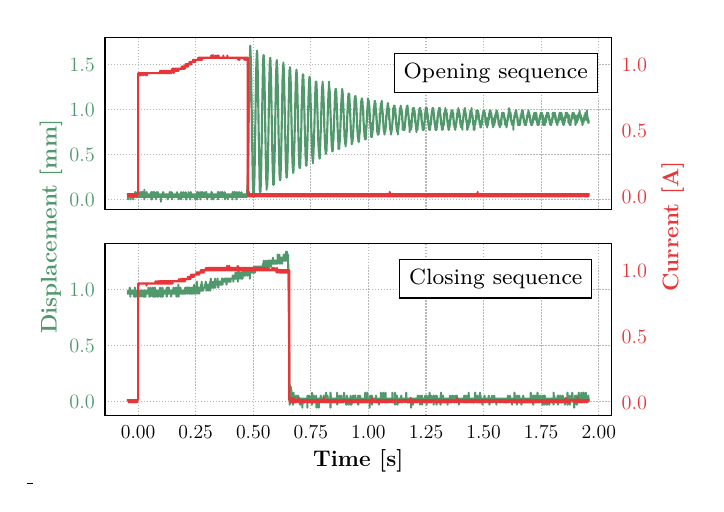
\begin{tikzpicture}
    \node[anchor=south west,inner sep=0] (graph) at (0,0) {\resizebox{0.7\textwidth}{!}{%% Creator: Matplotlib, PGF backend
%%
%% To include the figure in your LaTeX document, write
%%   \input{<filename>.pgf}
%%
%% Make sure the required packages are loaded in your preamble
%%   \usepackage{pgf}
%%
%% and, on pdftex
%%   \usepackage[utf8]{inputenc}\DeclareUnicodeCharacter{2212}{-}
%%
%% or, on luatex and xetex
%%   \usepackage{unicode-math}
%%
%% Figures using additional raster images can only be included by \input if
%% they are in the same directory as the main LaTeX file. For loading figures
%% from other directories you can use the `import` package
%%   \usepackage{import}
%%
%% and then include the figures with
%%   \import{<path to file>}{<filename>.pgf}
%%
%% Matplotlib used the following preamble
%%
\begingroup%
\makeatletter%
\begin{pgfpicture}%
\pgfpathrectangle{\pgfpointorigin}{\pgfqpoint{6.541944in}{4.466138in}}%
\pgfusepath{use as bounding box, clip}%
\begin{pgfscope}%
\pgfsetbuttcap%
\pgfsetmiterjoin%
\pgfsetlinewidth{0.000000pt}%
\definecolor{currentstroke}{rgb}{0.000000,0.000000,0.000000}%
\pgfsetstrokecolor{currentstroke}%
\pgfsetstrokeopacity{0.000000}%
\pgfsetdash{}{0pt}%
\pgfpathmoveto{\pgfqpoint{0.000000in}{0.000000in}}%
\pgfpathlineto{\pgfqpoint{6.541944in}{0.000000in}}%
\pgfpathlineto{\pgfqpoint{6.541944in}{4.466138in}}%
\pgfpathlineto{\pgfqpoint{0.000000in}{4.466138in}}%
\pgfpathclose%
\pgfusepath{}%
\end{pgfscope}%
\begin{pgfscope}%
\pgfsetbuttcap%
\pgfsetmiterjoin%
\pgfsetlinewidth{0.000000pt}%
\definecolor{currentstroke}{rgb}{0.000000,0.000000,0.000000}%
\pgfsetstrokecolor{currentstroke}%
\pgfsetstrokeopacity{0.000000}%
\pgfsetdash{}{0pt}%
\pgfpathmoveto{\pgfqpoint{0.756250in}{2.686138in}}%
\pgfpathlineto{\pgfqpoint{5.716250in}{2.686138in}}%
\pgfpathlineto{\pgfqpoint{5.716250in}{4.366138in}}%
\pgfpathlineto{\pgfqpoint{0.756250in}{4.366138in}}%
\pgfpathclose%
\pgfusepath{}%
\end{pgfscope}%
\begin{pgfscope}%
\pgfpathrectangle{\pgfqpoint{0.756250in}{2.686138in}}{\pgfqpoint{4.960000in}{1.680000in}}%
\pgfusepath{clip}%
\pgfsetbuttcap%
\pgfsetroundjoin%
\pgfsetlinewidth{0.803000pt}%
\definecolor{currentstroke}{rgb}{0.690196,0.690196,0.690196}%
\pgfsetstrokecolor{currentstroke}%
\pgfsetstrokeopacity{0.900000}%
\pgfsetdash{{0.800000pt}{1.320000pt}}{0.000000pt}%
\pgfpathmoveto{\pgfqpoint{1.080981in}{2.686138in}}%
\pgfpathlineto{\pgfqpoint{1.080981in}{4.366138in}}%
\pgfusepath{stroke}%
\end{pgfscope}%
\begin{pgfscope}%
\pgfsetbuttcap%
\pgfsetroundjoin%
\definecolor{currentfill}{rgb}{0.000000,0.000000,0.000000}%
\pgfsetfillcolor{currentfill}%
\pgfsetlinewidth{0.803000pt}%
\definecolor{currentstroke}{rgb}{0.000000,0.000000,0.000000}%
\pgfsetstrokecolor{currentstroke}%
\pgfsetdash{}{0pt}%
\pgfsys@defobject{currentmarker}{\pgfqpoint{0.000000in}{-0.048611in}}{\pgfqpoint{0.000000in}{0.000000in}}{%
\pgfpathmoveto{\pgfqpoint{0.000000in}{0.000000in}}%
\pgfpathlineto{\pgfqpoint{0.000000in}{-0.048611in}}%
\pgfusepath{stroke,fill}%
}%
\begin{pgfscope}%
\pgfsys@transformshift{1.080981in}{2.686138in}%
\pgfsys@useobject{currentmarker}{}%
\end{pgfscope}%
\end{pgfscope}%
\begin{pgfscope}%
\pgfpathrectangle{\pgfqpoint{0.756250in}{2.686138in}}{\pgfqpoint{4.960000in}{1.680000in}}%
\pgfusepath{clip}%
\pgfsetbuttcap%
\pgfsetroundjoin%
\pgfsetlinewidth{0.803000pt}%
\definecolor{currentstroke}{rgb}{0.690196,0.690196,0.690196}%
\pgfsetstrokecolor{currentstroke}%
\pgfsetstrokeopacity{0.900000}%
\pgfsetdash{{0.800000pt}{1.320000pt}}{0.000000pt}%
\pgfpathmoveto{\pgfqpoint{1.644604in}{2.686138in}}%
\pgfpathlineto{\pgfqpoint{1.644604in}{4.366138in}}%
\pgfusepath{stroke}%
\end{pgfscope}%
\begin{pgfscope}%
\pgfsetbuttcap%
\pgfsetroundjoin%
\definecolor{currentfill}{rgb}{0.000000,0.000000,0.000000}%
\pgfsetfillcolor{currentfill}%
\pgfsetlinewidth{0.803000pt}%
\definecolor{currentstroke}{rgb}{0.000000,0.000000,0.000000}%
\pgfsetstrokecolor{currentstroke}%
\pgfsetdash{}{0pt}%
\pgfsys@defobject{currentmarker}{\pgfqpoint{0.000000in}{-0.048611in}}{\pgfqpoint{0.000000in}{0.000000in}}{%
\pgfpathmoveto{\pgfqpoint{0.000000in}{0.000000in}}%
\pgfpathlineto{\pgfqpoint{0.000000in}{-0.048611in}}%
\pgfusepath{stroke,fill}%
}%
\begin{pgfscope}%
\pgfsys@transformshift{1.644604in}{2.686138in}%
\pgfsys@useobject{currentmarker}{}%
\end{pgfscope}%
\end{pgfscope}%
\begin{pgfscope}%
\pgfpathrectangle{\pgfqpoint{0.756250in}{2.686138in}}{\pgfqpoint{4.960000in}{1.680000in}}%
\pgfusepath{clip}%
\pgfsetbuttcap%
\pgfsetroundjoin%
\pgfsetlinewidth{0.803000pt}%
\definecolor{currentstroke}{rgb}{0.690196,0.690196,0.690196}%
\pgfsetstrokecolor{currentstroke}%
\pgfsetstrokeopacity{0.900000}%
\pgfsetdash{{0.800000pt}{1.320000pt}}{0.000000pt}%
\pgfpathmoveto{\pgfqpoint{2.208228in}{2.686138in}}%
\pgfpathlineto{\pgfqpoint{2.208228in}{4.366138in}}%
\pgfusepath{stroke}%
\end{pgfscope}%
\begin{pgfscope}%
\pgfsetbuttcap%
\pgfsetroundjoin%
\definecolor{currentfill}{rgb}{0.000000,0.000000,0.000000}%
\pgfsetfillcolor{currentfill}%
\pgfsetlinewidth{0.803000pt}%
\definecolor{currentstroke}{rgb}{0.000000,0.000000,0.000000}%
\pgfsetstrokecolor{currentstroke}%
\pgfsetdash{}{0pt}%
\pgfsys@defobject{currentmarker}{\pgfqpoint{0.000000in}{-0.048611in}}{\pgfqpoint{0.000000in}{0.000000in}}{%
\pgfpathmoveto{\pgfqpoint{0.000000in}{0.000000in}}%
\pgfpathlineto{\pgfqpoint{0.000000in}{-0.048611in}}%
\pgfusepath{stroke,fill}%
}%
\begin{pgfscope}%
\pgfsys@transformshift{2.208228in}{2.686138in}%
\pgfsys@useobject{currentmarker}{}%
\end{pgfscope}%
\end{pgfscope}%
\begin{pgfscope}%
\pgfpathrectangle{\pgfqpoint{0.756250in}{2.686138in}}{\pgfqpoint{4.960000in}{1.680000in}}%
\pgfusepath{clip}%
\pgfsetbuttcap%
\pgfsetroundjoin%
\pgfsetlinewidth{0.803000pt}%
\definecolor{currentstroke}{rgb}{0.690196,0.690196,0.690196}%
\pgfsetstrokecolor{currentstroke}%
\pgfsetstrokeopacity{0.900000}%
\pgfsetdash{{0.800000pt}{1.320000pt}}{0.000000pt}%
\pgfpathmoveto{\pgfqpoint{2.771852in}{2.686138in}}%
\pgfpathlineto{\pgfqpoint{2.771852in}{4.366138in}}%
\pgfusepath{stroke}%
\end{pgfscope}%
\begin{pgfscope}%
\pgfsetbuttcap%
\pgfsetroundjoin%
\definecolor{currentfill}{rgb}{0.000000,0.000000,0.000000}%
\pgfsetfillcolor{currentfill}%
\pgfsetlinewidth{0.803000pt}%
\definecolor{currentstroke}{rgb}{0.000000,0.000000,0.000000}%
\pgfsetstrokecolor{currentstroke}%
\pgfsetdash{}{0pt}%
\pgfsys@defobject{currentmarker}{\pgfqpoint{0.000000in}{-0.048611in}}{\pgfqpoint{0.000000in}{0.000000in}}{%
\pgfpathmoveto{\pgfqpoint{0.000000in}{0.000000in}}%
\pgfpathlineto{\pgfqpoint{0.000000in}{-0.048611in}}%
\pgfusepath{stroke,fill}%
}%
\begin{pgfscope}%
\pgfsys@transformshift{2.771852in}{2.686138in}%
\pgfsys@useobject{currentmarker}{}%
\end{pgfscope}%
\end{pgfscope}%
\begin{pgfscope}%
\pgfpathrectangle{\pgfqpoint{0.756250in}{2.686138in}}{\pgfqpoint{4.960000in}{1.680000in}}%
\pgfusepath{clip}%
\pgfsetbuttcap%
\pgfsetroundjoin%
\pgfsetlinewidth{0.803000pt}%
\definecolor{currentstroke}{rgb}{0.690196,0.690196,0.690196}%
\pgfsetstrokecolor{currentstroke}%
\pgfsetstrokeopacity{0.900000}%
\pgfsetdash{{0.800000pt}{1.320000pt}}{0.000000pt}%
\pgfpathmoveto{\pgfqpoint{3.335475in}{2.686138in}}%
\pgfpathlineto{\pgfqpoint{3.335475in}{4.366138in}}%
\pgfusepath{stroke}%
\end{pgfscope}%
\begin{pgfscope}%
\pgfsetbuttcap%
\pgfsetroundjoin%
\definecolor{currentfill}{rgb}{0.000000,0.000000,0.000000}%
\pgfsetfillcolor{currentfill}%
\pgfsetlinewidth{0.803000pt}%
\definecolor{currentstroke}{rgb}{0.000000,0.000000,0.000000}%
\pgfsetstrokecolor{currentstroke}%
\pgfsetdash{}{0pt}%
\pgfsys@defobject{currentmarker}{\pgfqpoint{0.000000in}{-0.048611in}}{\pgfqpoint{0.000000in}{0.000000in}}{%
\pgfpathmoveto{\pgfqpoint{0.000000in}{0.000000in}}%
\pgfpathlineto{\pgfqpoint{0.000000in}{-0.048611in}}%
\pgfusepath{stroke,fill}%
}%
\begin{pgfscope}%
\pgfsys@transformshift{3.335475in}{2.686138in}%
\pgfsys@useobject{currentmarker}{}%
\end{pgfscope}%
\end{pgfscope}%
\begin{pgfscope}%
\pgfpathrectangle{\pgfqpoint{0.756250in}{2.686138in}}{\pgfqpoint{4.960000in}{1.680000in}}%
\pgfusepath{clip}%
\pgfsetbuttcap%
\pgfsetroundjoin%
\pgfsetlinewidth{0.803000pt}%
\definecolor{currentstroke}{rgb}{0.690196,0.690196,0.690196}%
\pgfsetstrokecolor{currentstroke}%
\pgfsetstrokeopacity{0.900000}%
\pgfsetdash{{0.800000pt}{1.320000pt}}{0.000000pt}%
\pgfpathmoveto{\pgfqpoint{3.899099in}{2.686138in}}%
\pgfpathlineto{\pgfqpoint{3.899099in}{4.366138in}}%
\pgfusepath{stroke}%
\end{pgfscope}%
\begin{pgfscope}%
\pgfsetbuttcap%
\pgfsetroundjoin%
\definecolor{currentfill}{rgb}{0.000000,0.000000,0.000000}%
\pgfsetfillcolor{currentfill}%
\pgfsetlinewidth{0.803000pt}%
\definecolor{currentstroke}{rgb}{0.000000,0.000000,0.000000}%
\pgfsetstrokecolor{currentstroke}%
\pgfsetdash{}{0pt}%
\pgfsys@defobject{currentmarker}{\pgfqpoint{0.000000in}{-0.048611in}}{\pgfqpoint{0.000000in}{0.000000in}}{%
\pgfpathmoveto{\pgfqpoint{0.000000in}{0.000000in}}%
\pgfpathlineto{\pgfqpoint{0.000000in}{-0.048611in}}%
\pgfusepath{stroke,fill}%
}%
\begin{pgfscope}%
\pgfsys@transformshift{3.899099in}{2.686138in}%
\pgfsys@useobject{currentmarker}{}%
\end{pgfscope}%
\end{pgfscope}%
\begin{pgfscope}%
\pgfpathrectangle{\pgfqpoint{0.756250in}{2.686138in}}{\pgfqpoint{4.960000in}{1.680000in}}%
\pgfusepath{clip}%
\pgfsetbuttcap%
\pgfsetroundjoin%
\pgfsetlinewidth{0.803000pt}%
\definecolor{currentstroke}{rgb}{0.690196,0.690196,0.690196}%
\pgfsetstrokecolor{currentstroke}%
\pgfsetstrokeopacity{0.900000}%
\pgfsetdash{{0.800000pt}{1.320000pt}}{0.000000pt}%
\pgfpathmoveto{\pgfqpoint{4.462723in}{2.686138in}}%
\pgfpathlineto{\pgfqpoint{4.462723in}{4.366138in}}%
\pgfusepath{stroke}%
\end{pgfscope}%
\begin{pgfscope}%
\pgfsetbuttcap%
\pgfsetroundjoin%
\definecolor{currentfill}{rgb}{0.000000,0.000000,0.000000}%
\pgfsetfillcolor{currentfill}%
\pgfsetlinewidth{0.803000pt}%
\definecolor{currentstroke}{rgb}{0.000000,0.000000,0.000000}%
\pgfsetstrokecolor{currentstroke}%
\pgfsetdash{}{0pt}%
\pgfsys@defobject{currentmarker}{\pgfqpoint{0.000000in}{-0.048611in}}{\pgfqpoint{0.000000in}{0.000000in}}{%
\pgfpathmoveto{\pgfqpoint{0.000000in}{0.000000in}}%
\pgfpathlineto{\pgfqpoint{0.000000in}{-0.048611in}}%
\pgfusepath{stroke,fill}%
}%
\begin{pgfscope}%
\pgfsys@transformshift{4.462723in}{2.686138in}%
\pgfsys@useobject{currentmarker}{}%
\end{pgfscope}%
\end{pgfscope}%
\begin{pgfscope}%
\pgfpathrectangle{\pgfqpoint{0.756250in}{2.686138in}}{\pgfqpoint{4.960000in}{1.680000in}}%
\pgfusepath{clip}%
\pgfsetbuttcap%
\pgfsetroundjoin%
\pgfsetlinewidth{0.803000pt}%
\definecolor{currentstroke}{rgb}{0.690196,0.690196,0.690196}%
\pgfsetstrokecolor{currentstroke}%
\pgfsetstrokeopacity{0.900000}%
\pgfsetdash{{0.800000pt}{1.320000pt}}{0.000000pt}%
\pgfpathmoveto{\pgfqpoint{5.026346in}{2.686138in}}%
\pgfpathlineto{\pgfqpoint{5.026346in}{4.366138in}}%
\pgfusepath{stroke}%
\end{pgfscope}%
\begin{pgfscope}%
\pgfsetbuttcap%
\pgfsetroundjoin%
\definecolor{currentfill}{rgb}{0.000000,0.000000,0.000000}%
\pgfsetfillcolor{currentfill}%
\pgfsetlinewidth{0.803000pt}%
\definecolor{currentstroke}{rgb}{0.000000,0.000000,0.000000}%
\pgfsetstrokecolor{currentstroke}%
\pgfsetdash{}{0pt}%
\pgfsys@defobject{currentmarker}{\pgfqpoint{0.000000in}{-0.048611in}}{\pgfqpoint{0.000000in}{0.000000in}}{%
\pgfpathmoveto{\pgfqpoint{0.000000in}{0.000000in}}%
\pgfpathlineto{\pgfqpoint{0.000000in}{-0.048611in}}%
\pgfusepath{stroke,fill}%
}%
\begin{pgfscope}%
\pgfsys@transformshift{5.026346in}{2.686138in}%
\pgfsys@useobject{currentmarker}{}%
\end{pgfscope}%
\end{pgfscope}%
\begin{pgfscope}%
\pgfpathrectangle{\pgfqpoint{0.756250in}{2.686138in}}{\pgfqpoint{4.960000in}{1.680000in}}%
\pgfusepath{clip}%
\pgfsetbuttcap%
\pgfsetroundjoin%
\pgfsetlinewidth{0.803000pt}%
\definecolor{currentstroke}{rgb}{0.690196,0.690196,0.690196}%
\pgfsetstrokecolor{currentstroke}%
\pgfsetstrokeopacity{0.900000}%
\pgfsetdash{{0.800000pt}{1.320000pt}}{0.000000pt}%
\pgfpathmoveto{\pgfqpoint{5.589970in}{2.686138in}}%
\pgfpathlineto{\pgfqpoint{5.589970in}{4.366138in}}%
\pgfusepath{stroke}%
\end{pgfscope}%
\begin{pgfscope}%
\pgfsetbuttcap%
\pgfsetroundjoin%
\definecolor{currentfill}{rgb}{0.000000,0.000000,0.000000}%
\pgfsetfillcolor{currentfill}%
\pgfsetlinewidth{0.803000pt}%
\definecolor{currentstroke}{rgb}{0.000000,0.000000,0.000000}%
\pgfsetstrokecolor{currentstroke}%
\pgfsetdash{}{0pt}%
\pgfsys@defobject{currentmarker}{\pgfqpoint{0.000000in}{-0.048611in}}{\pgfqpoint{0.000000in}{0.000000in}}{%
\pgfpathmoveto{\pgfqpoint{0.000000in}{0.000000in}}%
\pgfpathlineto{\pgfqpoint{0.000000in}{-0.048611in}}%
\pgfusepath{stroke,fill}%
}%
\begin{pgfscope}%
\pgfsys@transformshift{5.589970in}{2.686138in}%
\pgfsys@useobject{currentmarker}{}%
\end{pgfscope}%
\end{pgfscope}%
\begin{pgfscope}%
\pgfpathrectangle{\pgfqpoint{0.756250in}{2.686138in}}{\pgfqpoint{4.960000in}{1.680000in}}%
\pgfusepath{clip}%
\pgfsetbuttcap%
\pgfsetroundjoin%
\pgfsetlinewidth{0.803000pt}%
\definecolor{currentstroke}{rgb}{0.690196,0.690196,0.690196}%
\pgfsetstrokecolor{currentstroke}%
\pgfsetstrokeopacity{0.900000}%
\pgfsetdash{{0.800000pt}{1.320000pt}}{0.000000pt}%
\pgfpathmoveto{\pgfqpoint{0.756250in}{2.785998in}}%
\pgfpathlineto{\pgfqpoint{5.716250in}{2.785998in}}%
\pgfusepath{stroke}%
\end{pgfscope}%
\begin{pgfscope}%
\pgfsetbuttcap%
\pgfsetroundjoin%
\definecolor{currentfill}{rgb}{0.000000,0.000000,0.000000}%
\pgfsetfillcolor{currentfill}%
\pgfsetlinewidth{0.803000pt}%
\definecolor{currentstroke}{rgb}{0.000000,0.000000,0.000000}%
\pgfsetstrokecolor{currentstroke}%
\pgfsetdash{}{0pt}%
\pgfsys@defobject{currentmarker}{\pgfqpoint{-0.048611in}{0.000000in}}{\pgfqpoint{-0.000000in}{0.000000in}}{%
\pgfpathmoveto{\pgfqpoint{-0.000000in}{0.000000in}}%
\pgfpathlineto{\pgfqpoint{-0.048611in}{0.000000in}}%
\pgfusepath{stroke,fill}%
}%
\begin{pgfscope}%
\pgfsys@transformshift{0.756250in}{2.785998in}%
\pgfsys@useobject{currentmarker}{}%
\end{pgfscope}%
\end{pgfscope}%
\begin{pgfscope}%
\definecolor{textcolor}{rgb}{0.317647,0.596078,0.423529}%
\pgfsetstrokecolor{textcolor}%
\pgfsetfillcolor{textcolor}%
\pgftext[x=0.408799in, y=2.716554in, left, base]{\color{textcolor}\rmfamily\fontsize{14.000000}{16.800000}\selectfont \(\displaystyle {0.0}\)}%
\end{pgfscope}%
\begin{pgfscope}%
\pgfpathrectangle{\pgfqpoint{0.756250in}{2.686138in}}{\pgfqpoint{4.960000in}{1.680000in}}%
\pgfusepath{clip}%
\pgfsetbuttcap%
\pgfsetroundjoin%
\pgfsetlinewidth{0.803000pt}%
\definecolor{currentstroke}{rgb}{0.690196,0.690196,0.690196}%
\pgfsetstrokecolor{currentstroke}%
\pgfsetstrokeopacity{0.900000}%
\pgfsetdash{{0.800000pt}{1.320000pt}}{0.000000pt}%
\pgfpathmoveto{\pgfqpoint{0.756250in}{3.226557in}}%
\pgfpathlineto{\pgfqpoint{5.716250in}{3.226557in}}%
\pgfusepath{stroke}%
\end{pgfscope}%
\begin{pgfscope}%
\pgfsetbuttcap%
\pgfsetroundjoin%
\definecolor{currentfill}{rgb}{0.000000,0.000000,0.000000}%
\pgfsetfillcolor{currentfill}%
\pgfsetlinewidth{0.803000pt}%
\definecolor{currentstroke}{rgb}{0.000000,0.000000,0.000000}%
\pgfsetstrokecolor{currentstroke}%
\pgfsetdash{}{0pt}%
\pgfsys@defobject{currentmarker}{\pgfqpoint{-0.048611in}{0.000000in}}{\pgfqpoint{-0.000000in}{0.000000in}}{%
\pgfpathmoveto{\pgfqpoint{-0.000000in}{0.000000in}}%
\pgfpathlineto{\pgfqpoint{-0.048611in}{0.000000in}}%
\pgfusepath{stroke,fill}%
}%
\begin{pgfscope}%
\pgfsys@transformshift{0.756250in}{3.226557in}%
\pgfsys@useobject{currentmarker}{}%
\end{pgfscope}%
\end{pgfscope}%
\begin{pgfscope}%
\definecolor{textcolor}{rgb}{0.317647,0.596078,0.423529}%
\pgfsetstrokecolor{textcolor}%
\pgfsetfillcolor{textcolor}%
\pgftext[x=0.408799in, y=3.157113in, left, base]{\color{textcolor}\rmfamily\fontsize{14.000000}{16.800000}\selectfont \(\displaystyle {0.5}\)}%
\end{pgfscope}%
\begin{pgfscope}%
\pgfpathrectangle{\pgfqpoint{0.756250in}{2.686138in}}{\pgfqpoint{4.960000in}{1.680000in}}%
\pgfusepath{clip}%
\pgfsetbuttcap%
\pgfsetroundjoin%
\pgfsetlinewidth{0.803000pt}%
\definecolor{currentstroke}{rgb}{0.690196,0.690196,0.690196}%
\pgfsetstrokecolor{currentstroke}%
\pgfsetstrokeopacity{0.900000}%
\pgfsetdash{{0.800000pt}{1.320000pt}}{0.000000pt}%
\pgfpathmoveto{\pgfqpoint{0.756250in}{3.667116in}}%
\pgfpathlineto{\pgfqpoint{5.716250in}{3.667116in}}%
\pgfusepath{stroke}%
\end{pgfscope}%
\begin{pgfscope}%
\pgfsetbuttcap%
\pgfsetroundjoin%
\definecolor{currentfill}{rgb}{0.000000,0.000000,0.000000}%
\pgfsetfillcolor{currentfill}%
\pgfsetlinewidth{0.803000pt}%
\definecolor{currentstroke}{rgb}{0.000000,0.000000,0.000000}%
\pgfsetstrokecolor{currentstroke}%
\pgfsetdash{}{0pt}%
\pgfsys@defobject{currentmarker}{\pgfqpoint{-0.048611in}{0.000000in}}{\pgfqpoint{-0.000000in}{0.000000in}}{%
\pgfpathmoveto{\pgfqpoint{-0.000000in}{0.000000in}}%
\pgfpathlineto{\pgfqpoint{-0.048611in}{0.000000in}}%
\pgfusepath{stroke,fill}%
}%
\begin{pgfscope}%
\pgfsys@transformshift{0.756250in}{3.667116in}%
\pgfsys@useobject{currentmarker}{}%
\end{pgfscope}%
\end{pgfscope}%
\begin{pgfscope}%
\definecolor{textcolor}{rgb}{0.317647,0.596078,0.423529}%
\pgfsetstrokecolor{textcolor}%
\pgfsetfillcolor{textcolor}%
\pgftext[x=0.408799in, y=3.597672in, left, base]{\color{textcolor}\rmfamily\fontsize{14.000000}{16.800000}\selectfont \(\displaystyle {1.0}\)}%
\end{pgfscope}%
\begin{pgfscope}%
\pgfpathrectangle{\pgfqpoint{0.756250in}{2.686138in}}{\pgfqpoint{4.960000in}{1.680000in}}%
\pgfusepath{clip}%
\pgfsetbuttcap%
\pgfsetroundjoin%
\pgfsetlinewidth{0.803000pt}%
\definecolor{currentstroke}{rgb}{0.690196,0.690196,0.690196}%
\pgfsetstrokecolor{currentstroke}%
\pgfsetstrokeopacity{0.900000}%
\pgfsetdash{{0.800000pt}{1.320000pt}}{0.000000pt}%
\pgfpathmoveto{\pgfqpoint{0.756250in}{4.107675in}}%
\pgfpathlineto{\pgfqpoint{5.716250in}{4.107675in}}%
\pgfusepath{stroke}%
\end{pgfscope}%
\begin{pgfscope}%
\pgfsetbuttcap%
\pgfsetroundjoin%
\definecolor{currentfill}{rgb}{0.000000,0.000000,0.000000}%
\pgfsetfillcolor{currentfill}%
\pgfsetlinewidth{0.803000pt}%
\definecolor{currentstroke}{rgb}{0.000000,0.000000,0.000000}%
\pgfsetstrokecolor{currentstroke}%
\pgfsetdash{}{0pt}%
\pgfsys@defobject{currentmarker}{\pgfqpoint{-0.048611in}{0.000000in}}{\pgfqpoint{-0.000000in}{0.000000in}}{%
\pgfpathmoveto{\pgfqpoint{-0.000000in}{0.000000in}}%
\pgfpathlineto{\pgfqpoint{-0.048611in}{0.000000in}}%
\pgfusepath{stroke,fill}%
}%
\begin{pgfscope}%
\pgfsys@transformshift{0.756250in}{4.107675in}%
\pgfsys@useobject{currentmarker}{}%
\end{pgfscope}%
\end{pgfscope}%
\begin{pgfscope}%
\definecolor{textcolor}{rgb}{0.317647,0.596078,0.423529}%
\pgfsetstrokecolor{textcolor}%
\pgfsetfillcolor{textcolor}%
\pgftext[x=0.408799in, y=4.038231in, left, base]{\color{textcolor}\rmfamily\fontsize{14.000000}{16.800000}\selectfont \(\displaystyle {1.5}\)}%
\end{pgfscope}%
\begin{pgfscope}%
\pgfpathrectangle{\pgfqpoint{0.756250in}{2.686138in}}{\pgfqpoint{4.960000in}{1.680000in}}%
\pgfusepath{clip}%
\pgfsetrectcap%
\pgfsetroundjoin%
\pgfsetlinewidth{1.505625pt}%
\definecolor{currentstroke}{rgb}{0.317647,0.596078,0.423529}%
\pgfsetstrokecolor{currentstroke}%
\pgfsetdash{}{0pt}%
\pgfpathmoveto{\pgfqpoint{0.981704in}{2.809495in}}%
\pgfpathlineto{\pgfqpoint{0.981884in}{2.809495in}}%
\pgfpathlineto{\pgfqpoint{0.982155in}{2.832991in}}%
\pgfpathlineto{\pgfqpoint{0.982245in}{2.809495in}}%
\pgfpathlineto{\pgfqpoint{0.982335in}{2.809495in}}%
\pgfpathlineto{\pgfqpoint{0.982696in}{2.832991in}}%
\pgfpathlineto{\pgfqpoint{0.983057in}{2.785998in}}%
\pgfpathlineto{\pgfqpoint{0.983418in}{2.832991in}}%
\pgfpathlineto{\pgfqpoint{0.983508in}{2.809495in}}%
\pgfpathlineto{\pgfqpoint{0.983778in}{2.832991in}}%
\pgfpathlineto{\pgfqpoint{0.983868in}{2.832991in}}%
\pgfpathlineto{\pgfqpoint{0.984319in}{2.809495in}}%
\pgfpathlineto{\pgfqpoint{0.984680in}{2.832991in}}%
\pgfpathlineto{\pgfqpoint{0.985041in}{2.809495in}}%
\pgfpathlineto{\pgfqpoint{0.985492in}{2.832991in}}%
\pgfpathlineto{\pgfqpoint{0.985852in}{2.832991in}}%
\pgfpathlineto{\pgfqpoint{0.986303in}{2.809495in}}%
\pgfpathlineto{\pgfqpoint{0.986484in}{2.809495in}}%
\pgfpathlineto{\pgfqpoint{0.986844in}{2.832991in}}%
\pgfpathlineto{\pgfqpoint{0.987205in}{2.809495in}}%
\pgfpathlineto{\pgfqpoint{0.987385in}{2.832991in}}%
\pgfpathlineto{\pgfqpoint{0.987566in}{2.809495in}}%
\pgfpathlineto{\pgfqpoint{0.987656in}{2.809495in}}%
\pgfpathlineto{\pgfqpoint{0.988107in}{2.832991in}}%
\pgfpathlineto{\pgfqpoint{0.988738in}{2.832991in}}%
\pgfpathlineto{\pgfqpoint{0.989009in}{2.809495in}}%
\pgfpathlineto{\pgfqpoint{0.989099in}{2.832991in}}%
\pgfpathlineto{\pgfqpoint{0.989189in}{2.832991in}}%
\pgfpathlineto{\pgfqpoint{0.989279in}{2.809495in}}%
\pgfpathlineto{\pgfqpoint{0.989550in}{2.832991in}}%
\pgfpathlineto{\pgfqpoint{0.989730in}{2.832991in}}%
\pgfpathlineto{\pgfqpoint{0.990181in}{2.809495in}}%
\pgfpathlineto{\pgfqpoint{0.990632in}{2.832991in}}%
\pgfpathlineto{\pgfqpoint{0.990902in}{2.832991in}}%
\pgfpathlineto{\pgfqpoint{0.990993in}{2.809495in}}%
\pgfpathlineto{\pgfqpoint{0.991263in}{2.832991in}}%
\pgfpathlineto{\pgfqpoint{0.991444in}{2.832991in}}%
\pgfpathlineto{\pgfqpoint{0.991894in}{2.809495in}}%
\pgfpathlineto{\pgfqpoint{0.992075in}{2.809495in}}%
\pgfpathlineto{\pgfqpoint{0.992436in}{2.832991in}}%
\pgfpathlineto{\pgfqpoint{0.992886in}{2.809495in}}%
\pgfpathlineto{\pgfqpoint{0.992977in}{2.809495in}}%
\pgfpathlineto{\pgfqpoint{0.993337in}{2.832991in}}%
\pgfpathlineto{\pgfqpoint{0.993788in}{2.809495in}}%
\pgfpathlineto{\pgfqpoint{0.994239in}{2.832991in}}%
\pgfpathlineto{\pgfqpoint{0.994329in}{2.832991in}}%
\pgfpathlineto{\pgfqpoint{0.994780in}{2.809495in}}%
\pgfpathlineto{\pgfqpoint{0.994870in}{2.809495in}}%
\pgfpathlineto{\pgfqpoint{0.995321in}{2.832991in}}%
\pgfpathlineto{\pgfqpoint{0.995772in}{2.809495in}}%
\pgfpathlineto{\pgfqpoint{0.996223in}{2.832991in}}%
\pgfpathlineto{\pgfqpoint{0.996403in}{2.832991in}}%
\pgfpathlineto{\pgfqpoint{0.996764in}{2.809495in}}%
\pgfpathlineto{\pgfqpoint{0.997035in}{2.832991in}}%
\pgfpathlineto{\pgfqpoint{0.997125in}{2.809495in}}%
\pgfpathlineto{\pgfqpoint{0.997305in}{2.809495in}}%
\pgfpathlineto{\pgfqpoint{0.997756in}{2.832991in}}%
\pgfpathlineto{\pgfqpoint{0.998297in}{2.832991in}}%
\pgfpathlineto{\pgfqpoint{0.998568in}{2.809495in}}%
\pgfpathlineto{\pgfqpoint{0.998658in}{2.832991in}}%
\pgfpathlineto{\pgfqpoint{0.998748in}{2.832991in}}%
\pgfpathlineto{\pgfqpoint{0.999199in}{2.809495in}}%
\pgfpathlineto{\pgfqpoint{0.999470in}{2.832991in}}%
\pgfpathlineto{\pgfqpoint{0.999560in}{2.809495in}}%
\pgfpathlineto{\pgfqpoint{0.999650in}{2.809495in}}%
\pgfpathlineto{\pgfqpoint{0.999920in}{2.832991in}}%
\pgfpathlineto{\pgfqpoint{1.000011in}{2.809495in}}%
\pgfpathlineto{\pgfqpoint{1.000191in}{2.809495in}}%
\pgfpathlineto{\pgfqpoint{1.000552in}{2.832991in}}%
\pgfpathlineto{\pgfqpoint{1.001003in}{2.809495in}}%
\pgfpathlineto{\pgfqpoint{1.001093in}{2.809495in}}%
\pgfpathlineto{\pgfqpoint{1.001544in}{2.832991in}}%
\pgfpathlineto{\pgfqpoint{1.001995in}{2.809495in}}%
\pgfpathlineto{\pgfqpoint{1.002175in}{2.809495in}}%
\pgfpathlineto{\pgfqpoint{1.002626in}{2.832991in}}%
\pgfpathlineto{\pgfqpoint{1.002806in}{2.832991in}}%
\pgfpathlineto{\pgfqpoint{1.003167in}{2.809495in}}%
\pgfpathlineto{\pgfqpoint{1.003618in}{2.832991in}}%
\pgfpathlineto{\pgfqpoint{1.003708in}{2.832991in}}%
\pgfpathlineto{\pgfqpoint{1.003798in}{2.809495in}}%
\pgfpathlineto{\pgfqpoint{1.004069in}{2.832991in}}%
\pgfpathlineto{\pgfqpoint{1.004790in}{2.832991in}}%
\pgfpathlineto{\pgfqpoint{1.005241in}{2.809495in}}%
\pgfpathlineto{\pgfqpoint{1.005331in}{2.809495in}}%
\pgfpathlineto{\pgfqpoint{1.005692in}{2.832991in}}%
\pgfpathlineto{\pgfqpoint{1.006053in}{2.809495in}}%
\pgfpathlineto{\pgfqpoint{1.006323in}{2.832991in}}%
\pgfpathlineto{\pgfqpoint{1.006413in}{2.809495in}}%
\pgfpathlineto{\pgfqpoint{1.006594in}{2.809495in}}%
\pgfpathlineto{\pgfqpoint{1.006954in}{2.832991in}}%
\pgfpathlineto{\pgfqpoint{1.007405in}{2.809495in}}%
\pgfpathlineto{\pgfqpoint{1.007676in}{2.832991in}}%
\pgfpathlineto{\pgfqpoint{1.007766in}{2.785998in}}%
\pgfpathlineto{\pgfqpoint{1.008037in}{2.809495in}}%
\pgfpathlineto{\pgfqpoint{1.008127in}{2.809495in}}%
\pgfpathlineto{\pgfqpoint{1.008578in}{2.832991in}}%
\pgfpathlineto{\pgfqpoint{1.009029in}{2.832991in}}%
\pgfpathlineto{\pgfqpoint{1.009299in}{2.809495in}}%
\pgfpathlineto{\pgfqpoint{1.009389in}{2.832991in}}%
\pgfpathlineto{\pgfqpoint{1.009660in}{2.832991in}}%
\pgfpathlineto{\pgfqpoint{1.010111in}{2.809495in}}%
\pgfpathlineto{\pgfqpoint{1.010471in}{2.832991in}}%
\pgfpathlineto{\pgfqpoint{1.010922in}{2.809495in}}%
\pgfpathlineto{\pgfqpoint{1.011013in}{2.809495in}}%
\pgfpathlineto{\pgfqpoint{1.011283in}{2.832991in}}%
\pgfpathlineto{\pgfqpoint{1.011373in}{2.809495in}}%
\pgfpathlineto{\pgfqpoint{1.011463in}{2.809495in}}%
\pgfpathlineto{\pgfqpoint{1.011914in}{2.832991in}}%
\pgfpathlineto{\pgfqpoint{1.012095in}{2.832991in}}%
\pgfpathlineto{\pgfqpoint{1.012185in}{2.809495in}}%
\pgfpathlineto{\pgfqpoint{1.012455in}{2.832991in}}%
\pgfpathlineto{\pgfqpoint{1.013087in}{2.832991in}}%
\pgfpathlineto{\pgfqpoint{1.013357in}{2.809495in}}%
\pgfpathlineto{\pgfqpoint{1.013447in}{2.832991in}}%
\pgfpathlineto{\pgfqpoint{1.013808in}{2.832991in}}%
\pgfpathlineto{\pgfqpoint{1.014169in}{2.809495in}}%
\pgfpathlineto{\pgfqpoint{1.014620in}{2.832991in}}%
\pgfpathlineto{\pgfqpoint{1.015071in}{2.809495in}}%
\pgfpathlineto{\pgfqpoint{1.015522in}{2.832991in}}%
\pgfpathlineto{\pgfqpoint{1.015792in}{2.832991in}}%
\pgfpathlineto{\pgfqpoint{1.016243in}{2.809495in}}%
\pgfpathlineto{\pgfqpoint{1.016784in}{2.809495in}}%
\pgfpathlineto{\pgfqpoint{1.017145in}{2.832991in}}%
\pgfpathlineto{\pgfqpoint{1.017596in}{2.809495in}}%
\pgfpathlineto{\pgfqpoint{1.018047in}{2.832991in}}%
\pgfpathlineto{\pgfqpoint{1.018497in}{2.809495in}}%
\pgfpathlineto{\pgfqpoint{1.018678in}{2.809495in}}%
\pgfpathlineto{\pgfqpoint{1.019039in}{2.832991in}}%
\pgfpathlineto{\pgfqpoint{1.019489in}{2.809495in}}%
\pgfpathlineto{\pgfqpoint{1.019850in}{2.832991in}}%
\pgfpathlineto{\pgfqpoint{1.020301in}{2.809495in}}%
\pgfpathlineto{\pgfqpoint{1.020391in}{2.809495in}}%
\pgfpathlineto{\pgfqpoint{1.020842in}{2.832991in}}%
\pgfpathlineto{\pgfqpoint{1.021203in}{2.809495in}}%
\pgfpathlineto{\pgfqpoint{1.021564in}{2.832991in}}%
\pgfpathlineto{\pgfqpoint{1.022014in}{2.809495in}}%
\pgfpathlineto{\pgfqpoint{1.022195in}{2.809495in}}%
\pgfpathlineto{\pgfqpoint{1.022465in}{2.832991in}}%
\pgfpathlineto{\pgfqpoint{1.022556in}{2.809495in}}%
\pgfpathlineto{\pgfqpoint{1.022826in}{2.809495in}}%
\pgfpathlineto{\pgfqpoint{1.023187in}{2.832991in}}%
\pgfpathlineto{\pgfqpoint{1.023638in}{2.809495in}}%
\pgfpathlineto{\pgfqpoint{1.023728in}{2.832991in}}%
\pgfpathlineto{\pgfqpoint{1.023998in}{2.809495in}}%
\pgfpathlineto{\pgfqpoint{1.024359in}{2.809495in}}%
\pgfpathlineto{\pgfqpoint{1.024810in}{2.832991in}}%
\pgfpathlineto{\pgfqpoint{1.025081in}{2.832991in}}%
\pgfpathlineto{\pgfqpoint{1.025532in}{2.809495in}}%
\pgfpathlineto{\pgfqpoint{1.025982in}{2.832991in}}%
\pgfpathlineto{\pgfqpoint{1.026073in}{2.832991in}}%
\pgfpathlineto{\pgfqpoint{1.026523in}{2.809495in}}%
\pgfpathlineto{\pgfqpoint{1.026794in}{2.809495in}}%
\pgfpathlineto{\pgfqpoint{1.027245in}{2.832991in}}%
\pgfpathlineto{\pgfqpoint{1.027425in}{2.832991in}}%
\pgfpathlineto{\pgfqpoint{1.027876in}{2.809495in}}%
\pgfpathlineto{\pgfqpoint{1.028057in}{2.809495in}}%
\pgfpathlineto{\pgfqpoint{1.028507in}{2.832991in}}%
\pgfpathlineto{\pgfqpoint{1.028598in}{2.832991in}}%
\pgfpathlineto{\pgfqpoint{1.028868in}{2.809495in}}%
\pgfpathlineto{\pgfqpoint{1.028958in}{2.832991in}}%
\pgfpathlineto{\pgfqpoint{1.029049in}{2.832991in}}%
\pgfpathlineto{\pgfqpoint{1.029499in}{2.809495in}}%
\pgfpathlineto{\pgfqpoint{1.029680in}{2.832991in}}%
\pgfpathlineto{\pgfqpoint{1.029860in}{2.809495in}}%
\pgfpathlineto{\pgfqpoint{1.030040in}{2.809495in}}%
\pgfpathlineto{\pgfqpoint{1.030491in}{2.832991in}}%
\pgfpathlineto{\pgfqpoint{1.030942in}{2.809495in}}%
\pgfpathlineto{\pgfqpoint{1.031393in}{2.832991in}}%
\pgfpathlineto{\pgfqpoint{1.031844in}{2.809495in}}%
\pgfpathlineto{\pgfqpoint{1.032205in}{2.832991in}}%
\pgfpathlineto{\pgfqpoint{1.032475in}{2.809495in}}%
\pgfpathlineto{\pgfqpoint{1.032566in}{2.832991in}}%
\pgfpathlineto{\pgfqpoint{1.032746in}{2.832991in}}%
\pgfpathlineto{\pgfqpoint{1.032926in}{2.809495in}}%
\pgfpathlineto{\pgfqpoint{1.033107in}{2.832991in}}%
\pgfpathlineto{\pgfqpoint{1.033197in}{2.832991in}}%
\pgfpathlineto{\pgfqpoint{1.033467in}{2.809495in}}%
\pgfpathlineto{\pgfqpoint{1.033558in}{2.832991in}}%
\pgfpathlineto{\pgfqpoint{1.033648in}{2.832991in}}%
\pgfpathlineto{\pgfqpoint{1.033738in}{2.785998in}}%
\pgfpathlineto{\pgfqpoint{1.034008in}{2.832991in}}%
\pgfpathlineto{\pgfqpoint{1.034369in}{2.809495in}}%
\pgfpathlineto{\pgfqpoint{1.034730in}{2.832991in}}%
\pgfpathlineto{\pgfqpoint{1.034820in}{2.809495in}}%
\pgfpathlineto{\pgfqpoint{1.035091in}{2.832991in}}%
\pgfpathlineto{\pgfqpoint{1.035181in}{2.832991in}}%
\pgfpathlineto{\pgfqpoint{1.035541in}{2.809495in}}%
\pgfpathlineto{\pgfqpoint{1.035992in}{2.832991in}}%
\pgfpathlineto{\pgfqpoint{1.036173in}{2.832991in}}%
\pgfpathlineto{\pgfqpoint{1.036624in}{2.809495in}}%
\pgfpathlineto{\pgfqpoint{1.037075in}{2.832991in}}%
\pgfpathlineto{\pgfqpoint{1.037525in}{2.809495in}}%
\pgfpathlineto{\pgfqpoint{1.037976in}{2.832991in}}%
\pgfpathlineto{\pgfqpoint{1.038337in}{2.809495in}}%
\pgfpathlineto{\pgfqpoint{1.038608in}{2.832991in}}%
\pgfpathlineto{\pgfqpoint{1.038698in}{2.809495in}}%
\pgfpathlineto{\pgfqpoint{1.038788in}{2.809495in}}%
\pgfpathlineto{\pgfqpoint{1.039239in}{2.832991in}}%
\pgfpathlineto{\pgfqpoint{1.039329in}{2.832991in}}%
\pgfpathlineto{\pgfqpoint{1.039780in}{2.809495in}}%
\pgfpathlineto{\pgfqpoint{1.039870in}{2.809495in}}%
\pgfpathlineto{\pgfqpoint{1.040231in}{2.832991in}}%
\pgfpathlineto{\pgfqpoint{1.040592in}{2.809495in}}%
\pgfpathlineto{\pgfqpoint{1.041042in}{2.832991in}}%
\pgfpathlineto{\pgfqpoint{1.041223in}{2.832991in}}%
\pgfpathlineto{\pgfqpoint{1.041674in}{2.809495in}}%
\pgfpathlineto{\pgfqpoint{1.042305in}{2.809495in}}%
\pgfpathlineto{\pgfqpoint{1.042756in}{2.832991in}}%
\pgfpathlineto{\pgfqpoint{1.042846in}{2.832991in}}%
\pgfpathlineto{\pgfqpoint{1.043297in}{2.809495in}}%
\pgfpathlineto{\pgfqpoint{1.043477in}{2.809495in}}%
\pgfpathlineto{\pgfqpoint{1.043838in}{2.832991in}}%
\pgfpathlineto{\pgfqpoint{1.044289in}{2.809495in}}%
\pgfpathlineto{\pgfqpoint{1.044559in}{2.809495in}}%
\pgfpathlineto{\pgfqpoint{1.045010in}{2.832991in}}%
\pgfpathlineto{\pgfqpoint{1.045461in}{2.809495in}}%
\pgfpathlineto{\pgfqpoint{1.045822in}{2.832991in}}%
\pgfpathlineto{\pgfqpoint{1.046273in}{2.809495in}}%
\pgfpathlineto{\pgfqpoint{1.046543in}{2.809495in}}%
\pgfpathlineto{\pgfqpoint{1.046634in}{2.832991in}}%
\pgfpathlineto{\pgfqpoint{1.046904in}{2.809495in}}%
\pgfpathlineto{\pgfqpoint{1.046994in}{2.809495in}}%
\pgfpathlineto{\pgfqpoint{1.047355in}{2.832991in}}%
\pgfpathlineto{\pgfqpoint{1.047716in}{2.809495in}}%
\pgfpathlineto{\pgfqpoint{1.048167in}{2.832991in}}%
\pgfpathlineto{\pgfqpoint{1.048257in}{2.809495in}}%
\pgfpathlineto{\pgfqpoint{1.048527in}{2.832991in}}%
\pgfpathlineto{\pgfqpoint{1.048618in}{2.832991in}}%
\pgfpathlineto{\pgfqpoint{1.048708in}{2.809495in}}%
\pgfpathlineto{\pgfqpoint{1.048978in}{2.832991in}}%
\pgfpathlineto{\pgfqpoint{1.049159in}{2.832991in}}%
\pgfpathlineto{\pgfqpoint{1.049519in}{2.809495in}}%
\pgfpathlineto{\pgfqpoint{1.049970in}{2.832991in}}%
\pgfpathlineto{\pgfqpoint{1.050151in}{2.832991in}}%
\pgfpathlineto{\pgfqpoint{1.050511in}{2.809495in}}%
\pgfpathlineto{\pgfqpoint{1.050782in}{2.832991in}}%
\pgfpathlineto{\pgfqpoint{1.050872in}{2.809495in}}%
\pgfpathlineto{\pgfqpoint{1.051143in}{2.809495in}}%
\pgfpathlineto{\pgfqpoint{1.051503in}{2.832991in}}%
\pgfpathlineto{\pgfqpoint{1.051954in}{2.809495in}}%
\pgfpathlineto{\pgfqpoint{1.052044in}{2.809495in}}%
\pgfpathlineto{\pgfqpoint{1.052405in}{2.856488in}}%
\pgfpathlineto{\pgfqpoint{1.052766in}{2.809495in}}%
\pgfpathlineto{\pgfqpoint{1.053217in}{2.832991in}}%
\pgfpathlineto{\pgfqpoint{1.053307in}{2.832991in}}%
\pgfpathlineto{\pgfqpoint{1.053758in}{2.809495in}}%
\pgfpathlineto{\pgfqpoint{1.053938in}{2.809495in}}%
\pgfpathlineto{\pgfqpoint{1.054389in}{2.832991in}}%
\pgfpathlineto{\pgfqpoint{1.054840in}{2.809495in}}%
\pgfpathlineto{\pgfqpoint{1.054930in}{2.856488in}}%
\pgfpathlineto{\pgfqpoint{1.055201in}{2.832991in}}%
\pgfpathlineto{\pgfqpoint{1.055381in}{2.809495in}}%
\pgfpathlineto{\pgfqpoint{1.055561in}{2.832991in}}%
\pgfpathlineto{\pgfqpoint{1.055832in}{2.832991in}}%
\pgfpathlineto{\pgfqpoint{1.056193in}{2.809495in}}%
\pgfpathlineto{\pgfqpoint{1.056644in}{2.832991in}}%
\pgfpathlineto{\pgfqpoint{1.057094in}{2.809495in}}%
\pgfpathlineto{\pgfqpoint{1.057185in}{2.809495in}}%
\pgfpathlineto{\pgfqpoint{1.057455in}{2.832991in}}%
\pgfpathlineto{\pgfqpoint{1.057545in}{2.809495in}}%
\pgfpathlineto{\pgfqpoint{1.057636in}{2.809495in}}%
\pgfpathlineto{\pgfqpoint{1.058086in}{2.832991in}}%
\pgfpathlineto{\pgfqpoint{1.058357in}{2.809495in}}%
\pgfpathlineto{\pgfqpoint{1.058447in}{2.832991in}}%
\pgfpathlineto{\pgfqpoint{1.059349in}{2.832991in}}%
\pgfpathlineto{\pgfqpoint{1.059800in}{2.809495in}}%
\pgfpathlineto{\pgfqpoint{1.059980in}{2.809495in}}%
\pgfpathlineto{\pgfqpoint{1.060251in}{2.832991in}}%
\pgfpathlineto{\pgfqpoint{1.060341in}{2.809495in}}%
\pgfpathlineto{\pgfqpoint{1.060431in}{2.809495in}}%
\pgfpathlineto{\pgfqpoint{1.060882in}{2.832991in}}%
\pgfpathlineto{\pgfqpoint{1.061333in}{2.832991in}}%
\pgfpathlineto{\pgfqpoint{1.061423in}{2.809495in}}%
\pgfpathlineto{\pgfqpoint{1.061694in}{2.832991in}}%
\pgfpathlineto{\pgfqpoint{1.062505in}{2.832991in}}%
\pgfpathlineto{\pgfqpoint{1.062595in}{2.809495in}}%
\pgfpathlineto{\pgfqpoint{1.062866in}{2.832991in}}%
\pgfpathlineto{\pgfqpoint{1.062956in}{2.832991in}}%
\pgfpathlineto{\pgfqpoint{1.063407in}{2.809495in}}%
\pgfpathlineto{\pgfqpoint{1.063678in}{2.832991in}}%
\pgfpathlineto{\pgfqpoint{1.063768in}{2.809495in}}%
\pgfpathlineto{\pgfqpoint{1.063948in}{2.809495in}}%
\pgfpathlineto{\pgfqpoint{1.064399in}{2.832991in}}%
\pgfpathlineto{\pgfqpoint{1.064760in}{2.809495in}}%
\pgfpathlineto{\pgfqpoint{1.065030in}{2.832991in}}%
\pgfpathlineto{\pgfqpoint{1.065120in}{2.809495in}}%
\pgfpathlineto{\pgfqpoint{1.065301in}{2.809495in}}%
\pgfpathlineto{\pgfqpoint{1.065571in}{2.832991in}}%
\pgfpathlineto{\pgfqpoint{1.065662in}{2.809495in}}%
\pgfpathlineto{\pgfqpoint{1.065752in}{2.809495in}}%
\pgfpathlineto{\pgfqpoint{1.065932in}{2.832991in}}%
\pgfpathlineto{\pgfqpoint{1.066112in}{2.809495in}}%
\pgfpathlineto{\pgfqpoint{1.066203in}{2.809495in}}%
\pgfpathlineto{\pgfqpoint{1.066653in}{2.832991in}}%
\pgfpathlineto{\pgfqpoint{1.066924in}{2.809495in}}%
\pgfpathlineto{\pgfqpoint{1.067014in}{2.832991in}}%
\pgfpathlineto{\pgfqpoint{1.067104in}{2.832991in}}%
\pgfpathlineto{\pgfqpoint{1.067195in}{2.809495in}}%
\pgfpathlineto{\pgfqpoint{1.067465in}{2.832991in}}%
\pgfpathlineto{\pgfqpoint{1.067645in}{2.832991in}}%
\pgfpathlineto{\pgfqpoint{1.068096in}{2.809495in}}%
\pgfpathlineto{\pgfqpoint{1.068187in}{2.809495in}}%
\pgfpathlineto{\pgfqpoint{1.068637in}{2.832991in}}%
\pgfpathlineto{\pgfqpoint{1.068728in}{2.832991in}}%
\pgfpathlineto{\pgfqpoint{1.068908in}{2.809495in}}%
\pgfpathlineto{\pgfqpoint{1.069088in}{2.832991in}}%
\pgfpathlineto{\pgfqpoint{1.069359in}{2.832991in}}%
\pgfpathlineto{\pgfqpoint{1.069810in}{2.809495in}}%
\pgfpathlineto{\pgfqpoint{1.070261in}{2.832991in}}%
\pgfpathlineto{\pgfqpoint{1.070621in}{2.832991in}}%
\pgfpathlineto{\pgfqpoint{1.070982in}{2.809495in}}%
\pgfpathlineto{\pgfqpoint{1.071433in}{2.832991in}}%
\pgfpathlineto{\pgfqpoint{1.071613in}{2.809495in}}%
\pgfpathlineto{\pgfqpoint{1.071794in}{2.832991in}}%
\pgfpathlineto{\pgfqpoint{1.072245in}{2.832991in}}%
\pgfpathlineto{\pgfqpoint{1.072696in}{2.809495in}}%
\pgfpathlineto{\pgfqpoint{1.072966in}{2.809495in}}%
\pgfpathlineto{\pgfqpoint{1.073417in}{2.856488in}}%
\pgfpathlineto{\pgfqpoint{1.073688in}{2.809495in}}%
\pgfpathlineto{\pgfqpoint{1.073868in}{2.832991in}}%
\pgfpathlineto{\pgfqpoint{1.073958in}{2.832991in}}%
\pgfpathlineto{\pgfqpoint{1.074138in}{2.809495in}}%
\pgfpathlineto{\pgfqpoint{1.074319in}{2.832991in}}%
\pgfpathlineto{\pgfqpoint{1.074589in}{2.832991in}}%
\pgfpathlineto{\pgfqpoint{1.075040in}{2.809495in}}%
\pgfpathlineto{\pgfqpoint{1.075491in}{2.832991in}}%
\pgfpathlineto{\pgfqpoint{1.075762in}{2.832991in}}%
\pgfpathlineto{\pgfqpoint{1.076213in}{2.809495in}}%
\pgfpathlineto{\pgfqpoint{1.076663in}{2.832991in}}%
\pgfpathlineto{\pgfqpoint{1.076754in}{2.832991in}}%
\pgfpathlineto{\pgfqpoint{1.077024in}{2.809495in}}%
\pgfpathlineto{\pgfqpoint{1.077114in}{2.832991in}}%
\pgfpathlineto{\pgfqpoint{1.077475in}{2.832991in}}%
\pgfpathlineto{\pgfqpoint{1.077565in}{2.856488in}}%
\pgfpathlineto{\pgfqpoint{1.077746in}{2.809495in}}%
\pgfpathlineto{\pgfqpoint{1.077836in}{2.832991in}}%
\pgfpathlineto{\pgfqpoint{1.077926in}{2.832991in}}%
\pgfpathlineto{\pgfqpoint{1.078287in}{2.809495in}}%
\pgfpathlineto{\pgfqpoint{1.078557in}{2.832991in}}%
\pgfpathlineto{\pgfqpoint{1.078647in}{2.809495in}}%
\pgfpathlineto{\pgfqpoint{1.078738in}{2.809495in}}%
\pgfpathlineto{\pgfqpoint{1.078828in}{2.832991in}}%
\pgfpathlineto{\pgfqpoint{1.079098in}{2.809495in}}%
\pgfpathlineto{\pgfqpoint{1.079369in}{2.809495in}}%
\pgfpathlineto{\pgfqpoint{1.079639in}{2.832991in}}%
\pgfpathlineto{\pgfqpoint{1.079730in}{2.809495in}}%
\pgfpathlineto{\pgfqpoint{1.079820in}{2.809495in}}%
\pgfpathlineto{\pgfqpoint{1.080271in}{2.832991in}}%
\pgfpathlineto{\pgfqpoint{1.080361in}{2.809495in}}%
\pgfpathlineto{\pgfqpoint{1.080631in}{2.832991in}}%
\pgfpathlineto{\pgfqpoint{1.080722in}{2.832991in}}%
\pgfpathlineto{\pgfqpoint{1.080992in}{2.809495in}}%
\pgfpathlineto{\pgfqpoint{1.081082in}{2.832991in}}%
\pgfpathlineto{\pgfqpoint{1.081172in}{2.832991in}}%
\pgfpathlineto{\pgfqpoint{1.081623in}{2.809495in}}%
\pgfpathlineto{\pgfqpoint{1.081714in}{2.809495in}}%
\pgfpathlineto{\pgfqpoint{1.082164in}{2.832991in}}%
\pgfpathlineto{\pgfqpoint{1.082615in}{2.809495in}}%
\pgfpathlineto{\pgfqpoint{1.082796in}{2.809495in}}%
\pgfpathlineto{\pgfqpoint{1.083247in}{2.832991in}}%
\pgfpathlineto{\pgfqpoint{1.083697in}{2.809495in}}%
\pgfpathlineto{\pgfqpoint{1.084239in}{2.809495in}}%
\pgfpathlineto{\pgfqpoint{1.084419in}{2.832991in}}%
\pgfpathlineto{\pgfqpoint{1.084599in}{2.809495in}}%
\pgfpathlineto{\pgfqpoint{1.084689in}{2.809495in}}%
\pgfpathlineto{\pgfqpoint{1.085050in}{2.832991in}}%
\pgfpathlineto{\pgfqpoint{1.085501in}{2.809495in}}%
\pgfpathlineto{\pgfqpoint{1.085952in}{2.832991in}}%
\pgfpathlineto{\pgfqpoint{1.086313in}{2.832991in}}%
\pgfpathlineto{\pgfqpoint{1.086764in}{2.809495in}}%
\pgfpathlineto{\pgfqpoint{1.087214in}{2.832991in}}%
\pgfpathlineto{\pgfqpoint{1.087485in}{2.832991in}}%
\pgfpathlineto{\pgfqpoint{1.087575in}{2.809495in}}%
\pgfpathlineto{\pgfqpoint{1.087846in}{2.832991in}}%
\pgfpathlineto{\pgfqpoint{1.088116in}{2.832991in}}%
\pgfpathlineto{\pgfqpoint{1.088567in}{2.809495in}}%
\pgfpathlineto{\pgfqpoint{1.088838in}{2.809495in}}%
\pgfpathlineto{\pgfqpoint{1.089289in}{2.832991in}}%
\pgfpathlineto{\pgfqpoint{1.089559in}{2.832991in}}%
\pgfpathlineto{\pgfqpoint{1.090010in}{2.809495in}}%
\pgfpathlineto{\pgfqpoint{1.090461in}{2.832991in}}%
\pgfpathlineto{\pgfqpoint{1.090912in}{2.809495in}}%
\pgfpathlineto{\pgfqpoint{1.091182in}{2.809495in}}%
\pgfpathlineto{\pgfqpoint{1.091633in}{2.832991in}}%
\pgfpathlineto{\pgfqpoint{1.091904in}{2.809495in}}%
\pgfpathlineto{\pgfqpoint{1.091994in}{2.832991in}}%
\pgfpathlineto{\pgfqpoint{1.092174in}{2.832991in}}%
\pgfpathlineto{\pgfqpoint{1.092355in}{2.809495in}}%
\pgfpathlineto{\pgfqpoint{1.092535in}{2.832991in}}%
\pgfpathlineto{\pgfqpoint{1.092625in}{2.832991in}}%
\pgfpathlineto{\pgfqpoint{1.092986in}{2.809495in}}%
\pgfpathlineto{\pgfqpoint{1.093437in}{2.832991in}}%
\pgfpathlineto{\pgfqpoint{1.093527in}{2.832991in}}%
\pgfpathlineto{\pgfqpoint{1.093798in}{2.809495in}}%
\pgfpathlineto{\pgfqpoint{1.093888in}{2.832991in}}%
\pgfpathlineto{\pgfqpoint{1.093978in}{2.832991in}}%
\pgfpathlineto{\pgfqpoint{1.094339in}{2.809495in}}%
\pgfpathlineto{\pgfqpoint{1.094519in}{2.832991in}}%
\pgfpathlineto{\pgfqpoint{1.094699in}{2.809495in}}%
\pgfpathlineto{\pgfqpoint{1.094880in}{2.809495in}}%
\pgfpathlineto{\pgfqpoint{1.095331in}{2.832991in}}%
\pgfpathlineto{\pgfqpoint{1.095421in}{2.832991in}}%
\pgfpathlineto{\pgfqpoint{1.095511in}{2.809495in}}%
\pgfpathlineto{\pgfqpoint{1.095782in}{2.832991in}}%
\pgfpathlineto{\pgfqpoint{1.095962in}{2.832991in}}%
\pgfpathlineto{\pgfqpoint{1.096232in}{2.809495in}}%
\pgfpathlineto{\pgfqpoint{1.096323in}{2.832991in}}%
\pgfpathlineto{\pgfqpoint{1.096413in}{2.832991in}}%
\pgfpathlineto{\pgfqpoint{1.096683in}{2.809495in}}%
\pgfpathlineto{\pgfqpoint{1.096774in}{2.832991in}}%
\pgfpathlineto{\pgfqpoint{1.096864in}{2.832991in}}%
\pgfpathlineto{\pgfqpoint{1.097315in}{2.809495in}}%
\pgfpathlineto{\pgfqpoint{1.097766in}{2.832991in}}%
\pgfpathlineto{\pgfqpoint{1.099389in}{2.832991in}}%
\pgfpathlineto{\pgfqpoint{1.099840in}{2.809495in}}%
\pgfpathlineto{\pgfqpoint{1.100020in}{2.809495in}}%
\pgfpathlineto{\pgfqpoint{1.100471in}{2.856488in}}%
\pgfpathlineto{\pgfqpoint{1.100922in}{2.832991in}}%
\pgfpathlineto{\pgfqpoint{1.101102in}{2.832991in}}%
\pgfpathlineto{\pgfqpoint{1.101373in}{2.809495in}}%
\pgfpathlineto{\pgfqpoint{1.101463in}{2.832991in}}%
\pgfpathlineto{\pgfqpoint{1.101643in}{2.832991in}}%
\pgfpathlineto{\pgfqpoint{1.102094in}{2.809495in}}%
\pgfpathlineto{\pgfqpoint{1.102545in}{2.832991in}}%
\pgfpathlineto{\pgfqpoint{1.102816in}{2.809495in}}%
\pgfpathlineto{\pgfqpoint{1.102906in}{2.832991in}}%
\pgfpathlineto{\pgfqpoint{1.103357in}{2.832991in}}%
\pgfpathlineto{\pgfqpoint{1.103627in}{2.809495in}}%
\pgfpathlineto{\pgfqpoint{1.103717in}{2.832991in}}%
\pgfpathlineto{\pgfqpoint{1.103808in}{2.832991in}}%
\pgfpathlineto{\pgfqpoint{1.104258in}{2.809495in}}%
\pgfpathlineto{\pgfqpoint{1.104349in}{2.809495in}}%
\pgfpathlineto{\pgfqpoint{1.104800in}{2.832991in}}%
\pgfpathlineto{\pgfqpoint{1.105250in}{2.809495in}}%
\pgfpathlineto{\pgfqpoint{1.105611in}{2.832991in}}%
\pgfpathlineto{\pgfqpoint{1.105701in}{2.809495in}}%
\pgfpathlineto{\pgfqpoint{1.105972in}{2.832991in}}%
\pgfpathlineto{\pgfqpoint{1.106152in}{2.832991in}}%
\pgfpathlineto{\pgfqpoint{1.106513in}{2.809495in}}%
\pgfpathlineto{\pgfqpoint{1.106964in}{2.832991in}}%
\pgfpathlineto{\pgfqpoint{1.107415in}{2.809495in}}%
\pgfpathlineto{\pgfqpoint{1.107775in}{2.832991in}}%
\pgfpathlineto{\pgfqpoint{1.108226in}{2.809495in}}%
\pgfpathlineto{\pgfqpoint{1.108677in}{2.832991in}}%
\pgfpathlineto{\pgfqpoint{1.108948in}{2.832991in}}%
\pgfpathlineto{\pgfqpoint{1.109309in}{2.809495in}}%
\pgfpathlineto{\pgfqpoint{1.109579in}{2.832991in}}%
\pgfpathlineto{\pgfqpoint{1.109669in}{2.809495in}}%
\pgfpathlineto{\pgfqpoint{1.109759in}{2.809495in}}%
\pgfpathlineto{\pgfqpoint{1.110120in}{2.832991in}}%
\pgfpathlineto{\pgfqpoint{1.110571in}{2.809495in}}%
\pgfpathlineto{\pgfqpoint{1.110661in}{2.809495in}}%
\pgfpathlineto{\pgfqpoint{1.111112in}{2.832991in}}%
\pgfpathlineto{\pgfqpoint{1.111563in}{2.809495in}}%
\pgfpathlineto{\pgfqpoint{1.111834in}{2.832991in}}%
\pgfpathlineto{\pgfqpoint{1.111924in}{2.809495in}}%
\pgfpathlineto{\pgfqpoint{1.112104in}{2.809495in}}%
\pgfpathlineto{\pgfqpoint{1.112375in}{2.832991in}}%
\pgfpathlineto{\pgfqpoint{1.112465in}{2.809495in}}%
\pgfpathlineto{\pgfqpoint{1.112555in}{2.809495in}}%
\pgfpathlineto{\pgfqpoint{1.112735in}{2.832991in}}%
\pgfpathlineto{\pgfqpoint{1.112916in}{2.809495in}}%
\pgfpathlineto{\pgfqpoint{1.113006in}{2.809495in}}%
\pgfpathlineto{\pgfqpoint{1.113367in}{2.832991in}}%
\pgfpathlineto{\pgfqpoint{1.113727in}{2.809495in}}%
\pgfpathlineto{\pgfqpoint{1.114178in}{2.832991in}}%
\pgfpathlineto{\pgfqpoint{1.114539in}{2.832991in}}%
\pgfpathlineto{\pgfqpoint{1.114990in}{2.809495in}}%
\pgfpathlineto{\pgfqpoint{1.115170in}{2.809495in}}%
\pgfpathlineto{\pgfqpoint{1.115260in}{2.832991in}}%
\pgfpathlineto{\pgfqpoint{1.115531in}{2.809495in}}%
\pgfpathlineto{\pgfqpoint{1.115711in}{2.809495in}}%
\pgfpathlineto{\pgfqpoint{1.116072in}{2.832991in}}%
\pgfpathlineto{\pgfqpoint{1.116343in}{2.809495in}}%
\pgfpathlineto{\pgfqpoint{1.116433in}{2.832991in}}%
\pgfpathlineto{\pgfqpoint{1.116703in}{2.832991in}}%
\pgfpathlineto{\pgfqpoint{1.117064in}{2.809495in}}%
\pgfpathlineto{\pgfqpoint{1.117515in}{2.856488in}}%
\pgfpathlineto{\pgfqpoint{1.117695in}{2.809495in}}%
\pgfpathlineto{\pgfqpoint{1.117876in}{2.832991in}}%
\pgfpathlineto{\pgfqpoint{1.117966in}{2.832991in}}%
\pgfpathlineto{\pgfqpoint{1.118417in}{2.809495in}}%
\pgfpathlineto{\pgfqpoint{1.118777in}{2.832991in}}%
\pgfpathlineto{\pgfqpoint{1.119228in}{2.809495in}}%
\pgfpathlineto{\pgfqpoint{1.119409in}{2.832991in}}%
\pgfpathlineto{\pgfqpoint{1.119589in}{2.809495in}}%
\pgfpathlineto{\pgfqpoint{1.119679in}{2.809495in}}%
\pgfpathlineto{\pgfqpoint{1.119860in}{2.832991in}}%
\pgfpathlineto{\pgfqpoint{1.120040in}{2.809495in}}%
\pgfpathlineto{\pgfqpoint{1.120310in}{2.809495in}}%
\pgfpathlineto{\pgfqpoint{1.120671in}{2.832991in}}%
\pgfpathlineto{\pgfqpoint{1.121122in}{2.809495in}}%
\pgfpathlineto{\pgfqpoint{1.121212in}{2.809495in}}%
\pgfpathlineto{\pgfqpoint{1.121302in}{2.832991in}}%
\pgfpathlineto{\pgfqpoint{1.121573in}{2.809495in}}%
\pgfpathlineto{\pgfqpoint{1.121753in}{2.809495in}}%
\pgfpathlineto{\pgfqpoint{1.122204in}{2.832991in}}%
\pgfpathlineto{\pgfqpoint{1.122565in}{2.809495in}}%
\pgfpathlineto{\pgfqpoint{1.122926in}{2.832991in}}%
\pgfpathlineto{\pgfqpoint{1.123377in}{2.809495in}}%
\pgfpathlineto{\pgfqpoint{1.123557in}{2.809495in}}%
\pgfpathlineto{\pgfqpoint{1.124008in}{2.832991in}}%
\pgfpathlineto{\pgfqpoint{1.124188in}{2.832991in}}%
\pgfpathlineto{\pgfqpoint{1.124549in}{2.809495in}}%
\pgfpathlineto{\pgfqpoint{1.124819in}{2.856488in}}%
\pgfpathlineto{\pgfqpoint{1.125000in}{2.832991in}}%
\pgfpathlineto{\pgfqpoint{1.125090in}{2.832991in}}%
\pgfpathlineto{\pgfqpoint{1.125451in}{2.809495in}}%
\pgfpathlineto{\pgfqpoint{1.125811in}{2.832991in}}%
\pgfpathlineto{\pgfqpoint{1.125992in}{2.809495in}}%
\pgfpathlineto{\pgfqpoint{1.126172in}{2.832991in}}%
\pgfpathlineto{\pgfqpoint{1.126262in}{2.832991in}}%
\pgfpathlineto{\pgfqpoint{1.126713in}{2.809495in}}%
\pgfpathlineto{\pgfqpoint{1.126894in}{2.809495in}}%
\pgfpathlineto{\pgfqpoint{1.127344in}{2.832991in}}%
\pgfpathlineto{\pgfqpoint{1.127435in}{2.832991in}}%
\pgfpathlineto{\pgfqpoint{1.127705in}{2.809495in}}%
\pgfpathlineto{\pgfqpoint{1.127795in}{2.832991in}}%
\pgfpathlineto{\pgfqpoint{1.127976in}{2.832991in}}%
\pgfpathlineto{\pgfqpoint{1.128427in}{2.809495in}}%
\pgfpathlineto{\pgfqpoint{1.128878in}{2.832991in}}%
\pgfpathlineto{\pgfqpoint{1.128968in}{2.809495in}}%
\pgfpathlineto{\pgfqpoint{1.129238in}{2.832991in}}%
\pgfpathlineto{\pgfqpoint{1.129509in}{2.832991in}}%
\pgfpathlineto{\pgfqpoint{1.129960in}{2.809495in}}%
\pgfpathlineto{\pgfqpoint{1.130230in}{2.832991in}}%
\pgfpathlineto{\pgfqpoint{1.130320in}{2.809495in}}%
\pgfpathlineto{\pgfqpoint{1.130591in}{2.809495in}}%
\pgfpathlineto{\pgfqpoint{1.130952in}{2.832991in}}%
\pgfpathlineto{\pgfqpoint{1.131312in}{2.809495in}}%
\pgfpathlineto{\pgfqpoint{1.131763in}{2.832991in}}%
\pgfpathlineto{\pgfqpoint{1.131853in}{2.809495in}}%
\pgfpathlineto{\pgfqpoint{1.132124in}{2.832991in}}%
\pgfpathlineto{\pgfqpoint{1.132395in}{2.832991in}}%
\pgfpathlineto{\pgfqpoint{1.132485in}{2.809495in}}%
\pgfpathlineto{\pgfqpoint{1.132755in}{2.832991in}}%
\pgfpathlineto{\pgfqpoint{1.132936in}{2.832991in}}%
\pgfpathlineto{\pgfqpoint{1.133387in}{2.809495in}}%
\pgfpathlineto{\pgfqpoint{1.133657in}{2.832991in}}%
\pgfpathlineto{\pgfqpoint{1.133747in}{2.809495in}}%
\pgfpathlineto{\pgfqpoint{1.134018in}{2.809495in}}%
\pgfpathlineto{\pgfqpoint{1.134288in}{2.832991in}}%
\pgfpathlineto{\pgfqpoint{1.134379in}{2.809495in}}%
\pgfpathlineto{\pgfqpoint{1.134559in}{2.809495in}}%
\pgfpathlineto{\pgfqpoint{1.134829in}{2.832991in}}%
\pgfpathlineto{\pgfqpoint{1.134920in}{2.809495in}}%
\pgfpathlineto{\pgfqpoint{1.135280in}{2.809495in}}%
\pgfpathlineto{\pgfqpoint{1.135731in}{2.832991in}}%
\pgfpathlineto{\pgfqpoint{1.136092in}{2.809495in}}%
\pgfpathlineto{\pgfqpoint{1.136453in}{2.832991in}}%
\pgfpathlineto{\pgfqpoint{1.136723in}{2.809495in}}%
\pgfpathlineto{\pgfqpoint{1.136813in}{2.832991in}}%
\pgfpathlineto{\pgfqpoint{1.136904in}{2.832991in}}%
\pgfpathlineto{\pgfqpoint{1.137354in}{2.809495in}}%
\pgfpathlineto{\pgfqpoint{1.137445in}{2.809495in}}%
\pgfpathlineto{\pgfqpoint{1.137896in}{2.832991in}}%
\pgfpathlineto{\pgfqpoint{1.138437in}{2.832991in}}%
\pgfpathlineto{\pgfqpoint{1.138888in}{2.809495in}}%
\pgfpathlineto{\pgfqpoint{1.139338in}{2.832991in}}%
\pgfpathlineto{\pgfqpoint{1.139429in}{2.832991in}}%
\pgfpathlineto{\pgfqpoint{1.139879in}{2.809495in}}%
\pgfpathlineto{\pgfqpoint{1.140330in}{2.832991in}}%
\pgfpathlineto{\pgfqpoint{1.140511in}{2.832991in}}%
\pgfpathlineto{\pgfqpoint{1.140781in}{2.809495in}}%
\pgfpathlineto{\pgfqpoint{1.140871in}{2.832991in}}%
\pgfpathlineto{\pgfqpoint{1.140962in}{2.832991in}}%
\pgfpathlineto{\pgfqpoint{1.141052in}{2.809495in}}%
\pgfpathlineto{\pgfqpoint{1.141322in}{2.832991in}}%
\pgfpathlineto{\pgfqpoint{1.141503in}{2.832991in}}%
\pgfpathlineto{\pgfqpoint{1.141863in}{2.785998in}}%
\pgfpathlineto{\pgfqpoint{1.142405in}{2.879984in}}%
\pgfpathlineto{\pgfqpoint{1.142855in}{2.809495in}}%
\pgfpathlineto{\pgfqpoint{1.142946in}{2.809495in}}%
\pgfpathlineto{\pgfqpoint{1.143396in}{2.832991in}}%
\pgfpathlineto{\pgfqpoint{1.143487in}{2.832991in}}%
\pgfpathlineto{\pgfqpoint{1.143938in}{2.809495in}}%
\pgfpathlineto{\pgfqpoint{1.144028in}{2.809495in}}%
\pgfpathlineto{\pgfqpoint{1.144388in}{2.832991in}}%
\pgfpathlineto{\pgfqpoint{1.144839in}{2.809495in}}%
\pgfpathlineto{\pgfqpoint{1.145290in}{2.809495in}}%
\pgfpathlineto{\pgfqpoint{1.145741in}{2.832991in}}%
\pgfpathlineto{\pgfqpoint{1.145831in}{2.832991in}}%
\pgfpathlineto{\pgfqpoint{1.146192in}{2.809495in}}%
\pgfpathlineto{\pgfqpoint{1.146553in}{2.832991in}}%
\pgfpathlineto{\pgfqpoint{1.146823in}{2.809495in}}%
\pgfpathlineto{\pgfqpoint{1.146914in}{2.832991in}}%
\pgfpathlineto{\pgfqpoint{1.147094in}{2.832991in}}%
\pgfpathlineto{\pgfqpoint{1.147545in}{2.809495in}}%
\pgfpathlineto{\pgfqpoint{1.147635in}{2.809495in}}%
\pgfpathlineto{\pgfqpoint{1.147996in}{2.832991in}}%
\pgfpathlineto{\pgfqpoint{1.148447in}{2.809495in}}%
\pgfpathlineto{\pgfqpoint{1.148807in}{2.809495in}}%
\pgfpathlineto{\pgfqpoint{1.148897in}{2.832991in}}%
\pgfpathlineto{\pgfqpoint{1.149168in}{2.809495in}}%
\pgfpathlineto{\pgfqpoint{1.149889in}{2.809495in}}%
\pgfpathlineto{\pgfqpoint{1.150250in}{2.832991in}}%
\pgfpathlineto{\pgfqpoint{1.150701in}{2.809495in}}%
\pgfpathlineto{\pgfqpoint{1.150791in}{2.809495in}}%
\pgfpathlineto{\pgfqpoint{1.151242in}{2.832991in}}%
\pgfpathlineto{\pgfqpoint{1.151422in}{2.809495in}}%
\pgfpathlineto{\pgfqpoint{1.151603in}{2.832991in}}%
\pgfpathlineto{\pgfqpoint{1.151693in}{2.832991in}}%
\pgfpathlineto{\pgfqpoint{1.152144in}{2.809495in}}%
\pgfpathlineto{\pgfqpoint{1.152595in}{2.832991in}}%
\pgfpathlineto{\pgfqpoint{1.152685in}{2.809495in}}%
\pgfpathlineto{\pgfqpoint{1.152956in}{2.832991in}}%
\pgfpathlineto{\pgfqpoint{1.153316in}{2.832991in}}%
\pgfpathlineto{\pgfqpoint{1.153406in}{2.809495in}}%
\pgfpathlineto{\pgfqpoint{1.153677in}{2.832991in}}%
\pgfpathlineto{\pgfqpoint{1.153767in}{2.832991in}}%
\pgfpathlineto{\pgfqpoint{1.154218in}{2.809495in}}%
\pgfpathlineto{\pgfqpoint{1.154308in}{2.809495in}}%
\pgfpathlineto{\pgfqpoint{1.154669in}{2.832991in}}%
\pgfpathlineto{\pgfqpoint{1.154759in}{2.809495in}}%
\pgfpathlineto{\pgfqpoint{1.155030in}{2.832991in}}%
\pgfpathlineto{\pgfqpoint{1.155481in}{2.832991in}}%
\pgfpathlineto{\pgfqpoint{1.155841in}{2.809495in}}%
\pgfpathlineto{\pgfqpoint{1.156292in}{2.832991in}}%
\pgfpathlineto{\pgfqpoint{1.156382in}{2.832991in}}%
\pgfpathlineto{\pgfqpoint{1.156563in}{2.809495in}}%
\pgfpathlineto{\pgfqpoint{1.156743in}{2.832991in}}%
\pgfpathlineto{\pgfqpoint{1.157014in}{2.832991in}}%
\pgfpathlineto{\pgfqpoint{1.157465in}{2.809495in}}%
\pgfpathlineto{\pgfqpoint{1.157735in}{2.832991in}}%
\pgfpathlineto{\pgfqpoint{1.157825in}{2.809495in}}%
\pgfpathlineto{\pgfqpoint{1.157915in}{2.809495in}}%
\pgfpathlineto{\pgfqpoint{1.158366in}{2.832991in}}%
\pgfpathlineto{\pgfqpoint{1.158817in}{2.809495in}}%
\pgfpathlineto{\pgfqpoint{1.158907in}{2.809495in}}%
\pgfpathlineto{\pgfqpoint{1.159358in}{2.832991in}}%
\pgfpathlineto{\pgfqpoint{1.159539in}{2.832991in}}%
\pgfpathlineto{\pgfqpoint{1.159899in}{2.809495in}}%
\pgfpathlineto{\pgfqpoint{1.160260in}{2.832991in}}%
\pgfpathlineto{\pgfqpoint{1.160711in}{2.809495in}}%
\pgfpathlineto{\pgfqpoint{1.160801in}{2.809495in}}%
\pgfpathlineto{\pgfqpoint{1.161072in}{2.832991in}}%
\pgfpathlineto{\pgfqpoint{1.161162in}{2.809495in}}%
\pgfpathlineto{\pgfqpoint{1.161523in}{2.809495in}}%
\pgfpathlineto{\pgfqpoint{1.161974in}{2.832991in}}%
\pgfpathlineto{\pgfqpoint{1.162424in}{2.809495in}}%
\pgfpathlineto{\pgfqpoint{1.162785in}{2.832991in}}%
\pgfpathlineto{\pgfqpoint{1.163236in}{2.809495in}}%
\pgfpathlineto{\pgfqpoint{1.163597in}{2.832991in}}%
\pgfpathlineto{\pgfqpoint{1.163687in}{2.809495in}}%
\pgfpathlineto{\pgfqpoint{1.163957in}{2.832991in}}%
\pgfpathlineto{\pgfqpoint{1.164048in}{2.832991in}}%
\pgfpathlineto{\pgfqpoint{1.164318in}{2.809495in}}%
\pgfpathlineto{\pgfqpoint{1.164408in}{2.832991in}}%
\pgfpathlineto{\pgfqpoint{1.164679in}{2.832991in}}%
\pgfpathlineto{\pgfqpoint{1.164859in}{2.856488in}}%
\pgfpathlineto{\pgfqpoint{1.165130in}{2.809495in}}%
\pgfpathlineto{\pgfqpoint{1.165581in}{2.832991in}}%
\pgfpathlineto{\pgfqpoint{1.166032in}{2.809495in}}%
\pgfpathlineto{\pgfqpoint{1.166392in}{2.832991in}}%
\pgfpathlineto{\pgfqpoint{1.166843in}{2.809495in}}%
\pgfpathlineto{\pgfqpoint{1.167114in}{2.832991in}}%
\pgfpathlineto{\pgfqpoint{1.167204in}{2.809495in}}%
\pgfpathlineto{\pgfqpoint{1.167384in}{2.809495in}}%
\pgfpathlineto{\pgfqpoint{1.167474in}{2.832991in}}%
\pgfpathlineto{\pgfqpoint{1.167745in}{2.809495in}}%
\pgfpathlineto{\pgfqpoint{1.167835in}{2.809495in}}%
\pgfpathlineto{\pgfqpoint{1.168106in}{2.832991in}}%
\pgfpathlineto{\pgfqpoint{1.168196in}{2.809495in}}%
\pgfpathlineto{\pgfqpoint{1.168286in}{2.809495in}}%
\pgfpathlineto{\pgfqpoint{1.168647in}{2.832991in}}%
\pgfpathlineto{\pgfqpoint{1.169008in}{2.809495in}}%
\pgfpathlineto{\pgfqpoint{1.169098in}{2.832991in}}%
\pgfpathlineto{\pgfqpoint{1.169368in}{2.809495in}}%
\pgfpathlineto{\pgfqpoint{1.169458in}{2.809495in}}%
\pgfpathlineto{\pgfqpoint{1.169819in}{2.832991in}}%
\pgfpathlineto{\pgfqpoint{1.170180in}{2.809495in}}%
\pgfpathlineto{\pgfqpoint{1.170631in}{2.832991in}}%
\pgfpathlineto{\pgfqpoint{1.170721in}{2.832991in}}%
\pgfpathlineto{\pgfqpoint{1.171172in}{2.809495in}}%
\pgfpathlineto{\pgfqpoint{1.171442in}{2.832991in}}%
\pgfpathlineto{\pgfqpoint{1.171533in}{2.809495in}}%
\pgfpathlineto{\pgfqpoint{1.171623in}{2.809495in}}%
\pgfpathlineto{\pgfqpoint{1.172074in}{2.832991in}}%
\pgfpathlineto{\pgfqpoint{1.172434in}{2.809495in}}%
\pgfpathlineto{\pgfqpoint{1.172795in}{2.832991in}}%
\pgfpathlineto{\pgfqpoint{1.173246in}{2.809495in}}%
\pgfpathlineto{\pgfqpoint{1.173426in}{2.809495in}}%
\pgfpathlineto{\pgfqpoint{1.173517in}{2.832991in}}%
\pgfpathlineto{\pgfqpoint{1.173787in}{2.809495in}}%
\pgfpathlineto{\pgfqpoint{1.174238in}{2.809495in}}%
\pgfpathlineto{\pgfqpoint{1.174599in}{2.832991in}}%
\pgfpathlineto{\pgfqpoint{1.174959in}{2.809495in}}%
\pgfpathlineto{\pgfqpoint{1.175410in}{2.832991in}}%
\pgfpathlineto{\pgfqpoint{1.175771in}{2.809495in}}%
\pgfpathlineto{\pgfqpoint{1.175951in}{2.832991in}}%
\pgfpathlineto{\pgfqpoint{1.176132in}{2.809495in}}%
\pgfpathlineto{\pgfqpoint{1.176402in}{2.809495in}}%
\pgfpathlineto{\pgfqpoint{1.176583in}{2.832991in}}%
\pgfpathlineto{\pgfqpoint{1.176763in}{2.809495in}}%
\pgfpathlineto{\pgfqpoint{1.177665in}{2.809495in}}%
\pgfpathlineto{\pgfqpoint{1.177845in}{2.832991in}}%
\pgfpathlineto{\pgfqpoint{1.178026in}{2.809495in}}%
\pgfpathlineto{\pgfqpoint{1.178296in}{2.809495in}}%
\pgfpathlineto{\pgfqpoint{1.178657in}{2.832991in}}%
\pgfpathlineto{\pgfqpoint{1.179108in}{2.809495in}}%
\pgfpathlineto{\pgfqpoint{1.179468in}{2.809495in}}%
\pgfpathlineto{\pgfqpoint{1.179649in}{2.832991in}}%
\pgfpathlineto{\pgfqpoint{1.179829in}{2.809495in}}%
\pgfpathlineto{\pgfqpoint{1.179919in}{2.809495in}}%
\pgfpathlineto{\pgfqpoint{1.180370in}{2.832991in}}%
\pgfpathlineto{\pgfqpoint{1.180821in}{2.809495in}}%
\pgfpathlineto{\pgfqpoint{1.180911in}{2.832991in}}%
\pgfpathlineto{\pgfqpoint{1.181182in}{2.809495in}}%
\pgfpathlineto{\pgfqpoint{1.181362in}{2.809495in}}%
\pgfpathlineto{\pgfqpoint{1.181723in}{2.832991in}}%
\pgfpathlineto{\pgfqpoint{1.182084in}{2.809495in}}%
\pgfpathlineto{\pgfqpoint{1.182535in}{2.832991in}}%
\pgfpathlineto{\pgfqpoint{1.182715in}{2.832991in}}%
\pgfpathlineto{\pgfqpoint{1.183166in}{2.809495in}}%
\pgfpathlineto{\pgfqpoint{1.183436in}{2.809495in}}%
\pgfpathlineto{\pgfqpoint{1.183797in}{2.832991in}}%
\pgfpathlineto{\pgfqpoint{1.184248in}{2.809495in}}%
\pgfpathlineto{\pgfqpoint{1.184428in}{2.809495in}}%
\pgfpathlineto{\pgfqpoint{1.184518in}{2.832991in}}%
\pgfpathlineto{\pgfqpoint{1.184789in}{2.809495in}}%
\pgfpathlineto{\pgfqpoint{1.184879in}{2.809495in}}%
\pgfpathlineto{\pgfqpoint{1.185330in}{2.832991in}}%
\pgfpathlineto{\pgfqpoint{1.185781in}{2.809495in}}%
\pgfpathlineto{\pgfqpoint{1.186142in}{2.832991in}}%
\pgfpathlineto{\pgfqpoint{1.186593in}{2.809495in}}%
\pgfpathlineto{\pgfqpoint{1.186683in}{2.832991in}}%
\pgfpathlineto{\pgfqpoint{1.186953in}{2.809495in}}%
\pgfpathlineto{\pgfqpoint{1.187134in}{2.809495in}}%
\pgfpathlineto{\pgfqpoint{1.187494in}{2.832991in}}%
\pgfpathlineto{\pgfqpoint{1.187945in}{2.809495in}}%
\pgfpathlineto{\pgfqpoint{1.188035in}{2.809495in}}%
\pgfpathlineto{\pgfqpoint{1.188306in}{2.832991in}}%
\pgfpathlineto{\pgfqpoint{1.188396in}{2.809495in}}%
\pgfpathlineto{\pgfqpoint{1.188486in}{2.809495in}}%
\pgfpathlineto{\pgfqpoint{1.188667in}{2.832991in}}%
\pgfpathlineto{\pgfqpoint{1.188847in}{2.809495in}}%
\pgfpathlineto{\pgfqpoint{1.188937in}{2.809495in}}%
\pgfpathlineto{\pgfqpoint{1.189298in}{2.832991in}}%
\pgfpathlineto{\pgfqpoint{1.189749in}{2.809495in}}%
\pgfpathlineto{\pgfqpoint{1.189839in}{2.809495in}}%
\pgfpathlineto{\pgfqpoint{1.190110in}{2.832991in}}%
\pgfpathlineto{\pgfqpoint{1.190200in}{2.809495in}}%
\pgfpathlineto{\pgfqpoint{1.190290in}{2.809495in}}%
\pgfpathlineto{\pgfqpoint{1.190741in}{2.832991in}}%
\pgfpathlineto{\pgfqpoint{1.190831in}{2.832991in}}%
\pgfpathlineto{\pgfqpoint{1.191282in}{2.809495in}}%
\pgfpathlineto{\pgfqpoint{1.191372in}{2.809495in}}%
\pgfpathlineto{\pgfqpoint{1.191823in}{2.832991in}}%
\pgfpathlineto{\pgfqpoint{1.192094in}{2.809495in}}%
\pgfpathlineto{\pgfqpoint{1.192184in}{2.832991in}}%
\pgfpathlineto{\pgfqpoint{1.192364in}{2.832991in}}%
\pgfpathlineto{\pgfqpoint{1.192815in}{2.809495in}}%
\pgfpathlineto{\pgfqpoint{1.193266in}{2.832991in}}%
\pgfpathlineto{\pgfqpoint{1.193717in}{2.809495in}}%
\pgfpathlineto{\pgfqpoint{1.194168in}{2.832991in}}%
\pgfpathlineto{\pgfqpoint{1.194348in}{2.832991in}}%
\pgfpathlineto{\pgfqpoint{1.194799in}{2.809495in}}%
\pgfpathlineto{\pgfqpoint{1.195070in}{2.832991in}}%
\pgfpathlineto{\pgfqpoint{1.195160in}{2.809495in}}%
\pgfpathlineto{\pgfqpoint{1.195250in}{2.809495in}}%
\pgfpathlineto{\pgfqpoint{1.195520in}{2.832991in}}%
\pgfpathlineto{\pgfqpoint{1.195611in}{2.809495in}}%
\pgfpathlineto{\pgfqpoint{1.195701in}{2.809495in}}%
\pgfpathlineto{\pgfqpoint{1.195791in}{2.832991in}}%
\pgfpathlineto{\pgfqpoint{1.196061in}{2.809495in}}%
\pgfpathlineto{\pgfqpoint{1.197053in}{2.809495in}}%
\pgfpathlineto{\pgfqpoint{1.197414in}{2.832991in}}%
\pgfpathlineto{\pgfqpoint{1.197865in}{2.809495in}}%
\pgfpathlineto{\pgfqpoint{1.198316in}{2.809495in}}%
\pgfpathlineto{\pgfqpoint{1.198587in}{2.832991in}}%
\pgfpathlineto{\pgfqpoint{1.198677in}{2.809495in}}%
\pgfpathlineto{\pgfqpoint{1.198857in}{2.809495in}}%
\pgfpathlineto{\pgfqpoint{1.199308in}{2.832991in}}%
\pgfpathlineto{\pgfqpoint{1.199579in}{2.832991in}}%
\pgfpathlineto{\pgfqpoint{1.200029in}{2.809495in}}%
\pgfpathlineto{\pgfqpoint{1.200390in}{2.832991in}}%
\pgfpathlineto{\pgfqpoint{1.200751in}{2.809495in}}%
\pgfpathlineto{\pgfqpoint{1.201202in}{2.832991in}}%
\pgfpathlineto{\pgfqpoint{1.201292in}{2.832991in}}%
\pgfpathlineto{\pgfqpoint{1.201743in}{2.809495in}}%
\pgfpathlineto{\pgfqpoint{1.202013in}{2.809495in}}%
\pgfpathlineto{\pgfqpoint{1.202464in}{2.832991in}}%
\pgfpathlineto{\pgfqpoint{1.203096in}{2.832991in}}%
\pgfpathlineto{\pgfqpoint{1.203456in}{2.809495in}}%
\pgfpathlineto{\pgfqpoint{1.203907in}{2.832991in}}%
\pgfpathlineto{\pgfqpoint{1.204358in}{2.809495in}}%
\pgfpathlineto{\pgfqpoint{1.204719in}{2.832991in}}%
\pgfpathlineto{\pgfqpoint{1.205079in}{2.809495in}}%
\pgfpathlineto{\pgfqpoint{1.205530in}{2.832991in}}%
\pgfpathlineto{\pgfqpoint{1.205981in}{2.809495in}}%
\pgfpathlineto{\pgfqpoint{1.206252in}{2.832991in}}%
\pgfpathlineto{\pgfqpoint{1.206342in}{2.809495in}}%
\pgfpathlineto{\pgfqpoint{1.206432in}{2.809495in}}%
\pgfpathlineto{\pgfqpoint{1.206883in}{2.832991in}}%
\pgfpathlineto{\pgfqpoint{1.207334in}{2.809495in}}%
\pgfpathlineto{\pgfqpoint{1.207785in}{2.809495in}}%
\pgfpathlineto{\pgfqpoint{1.208236in}{2.832991in}}%
\pgfpathlineto{\pgfqpoint{1.208416in}{2.809495in}}%
\pgfpathlineto{\pgfqpoint{1.208596in}{2.832991in}}%
\pgfpathlineto{\pgfqpoint{1.208687in}{2.832991in}}%
\pgfpathlineto{\pgfqpoint{1.208867in}{2.809495in}}%
\pgfpathlineto{\pgfqpoint{1.209047in}{2.832991in}}%
\pgfpathlineto{\pgfqpoint{1.209138in}{2.832991in}}%
\pgfpathlineto{\pgfqpoint{1.209408in}{2.856488in}}%
\pgfpathlineto{\pgfqpoint{1.209588in}{2.809495in}}%
\pgfpathlineto{\pgfqpoint{1.209679in}{2.809495in}}%
\pgfpathlineto{\pgfqpoint{1.210039in}{2.832991in}}%
\pgfpathlineto{\pgfqpoint{1.210400in}{2.785998in}}%
\pgfpathlineto{\pgfqpoint{1.210761in}{2.832991in}}%
\pgfpathlineto{\pgfqpoint{1.211212in}{2.809495in}}%
\pgfpathlineto{\pgfqpoint{1.211392in}{2.809495in}}%
\pgfpathlineto{\pgfqpoint{1.211753in}{2.832991in}}%
\pgfpathlineto{\pgfqpoint{1.212113in}{2.809495in}}%
\pgfpathlineto{\pgfqpoint{1.212384in}{2.832991in}}%
\pgfpathlineto{\pgfqpoint{1.212474in}{2.809495in}}%
\pgfpathlineto{\pgfqpoint{1.212564in}{2.809495in}}%
\pgfpathlineto{\pgfqpoint{1.212925in}{2.832991in}}%
\pgfpathlineto{\pgfqpoint{1.213196in}{2.809495in}}%
\pgfpathlineto{\pgfqpoint{1.213286in}{2.832991in}}%
\pgfpathlineto{\pgfqpoint{1.213376in}{2.832991in}}%
\pgfpathlineto{\pgfqpoint{1.213556in}{2.809495in}}%
\pgfpathlineto{\pgfqpoint{1.213737in}{2.832991in}}%
\pgfpathlineto{\pgfqpoint{1.214007in}{2.832991in}}%
\pgfpathlineto{\pgfqpoint{1.214188in}{2.809495in}}%
\pgfpathlineto{\pgfqpoint{1.214368in}{2.832991in}}%
\pgfpathlineto{\pgfqpoint{1.214548in}{2.832991in}}%
\pgfpathlineto{\pgfqpoint{1.214909in}{2.809495in}}%
\pgfpathlineto{\pgfqpoint{1.215270in}{2.856488in}}%
\pgfpathlineto{\pgfqpoint{1.215180in}{2.785998in}}%
\pgfpathlineto{\pgfqpoint{1.215360in}{2.832991in}}%
\pgfpathlineto{\pgfqpoint{1.215631in}{2.832991in}}%
\pgfpathlineto{\pgfqpoint{1.215991in}{2.809495in}}%
\pgfpathlineto{\pgfqpoint{1.216442in}{2.832991in}}%
\pgfpathlineto{\pgfqpoint{1.216713in}{2.832991in}}%
\pgfpathlineto{\pgfqpoint{1.217073in}{2.809495in}}%
\pgfpathlineto{\pgfqpoint{1.217524in}{2.832991in}}%
\pgfpathlineto{\pgfqpoint{1.217975in}{2.809495in}}%
\pgfpathlineto{\pgfqpoint{1.218336in}{2.832991in}}%
\pgfpathlineto{\pgfqpoint{1.218426in}{2.809495in}}%
\pgfpathlineto{\pgfqpoint{1.218697in}{2.832991in}}%
\pgfpathlineto{\pgfqpoint{1.218787in}{2.832991in}}%
\pgfpathlineto{\pgfqpoint{1.218877in}{2.809495in}}%
\pgfpathlineto{\pgfqpoint{1.219148in}{2.832991in}}%
\pgfpathlineto{\pgfqpoint{1.219689in}{2.832991in}}%
\pgfpathlineto{\pgfqpoint{1.220049in}{2.809495in}}%
\pgfpathlineto{\pgfqpoint{1.220500in}{2.832991in}}%
\pgfpathlineto{\pgfqpoint{1.220771in}{2.832991in}}%
\pgfpathlineto{\pgfqpoint{1.221222in}{2.809495in}}%
\pgfpathlineto{\pgfqpoint{1.221402in}{2.832991in}}%
\pgfpathlineto{\pgfqpoint{1.221582in}{2.809495in}}%
\pgfpathlineto{\pgfqpoint{1.221763in}{2.809495in}}%
\pgfpathlineto{\pgfqpoint{1.222214in}{2.832991in}}%
\pgfpathlineto{\pgfqpoint{1.222484in}{2.832991in}}%
\pgfpathlineto{\pgfqpoint{1.222935in}{2.809495in}}%
\pgfpathlineto{\pgfqpoint{1.223386in}{2.832991in}}%
\pgfpathlineto{\pgfqpoint{1.223747in}{2.832991in}}%
\pgfpathlineto{\pgfqpoint{1.224198in}{2.809495in}}%
\pgfpathlineto{\pgfqpoint{1.224648in}{2.832991in}}%
\pgfpathlineto{\pgfqpoint{1.224829in}{2.832991in}}%
\pgfpathlineto{\pgfqpoint{1.224919in}{2.809495in}}%
\pgfpathlineto{\pgfqpoint{1.225190in}{2.832991in}}%
\pgfpathlineto{\pgfqpoint{1.225280in}{2.832991in}}%
\pgfpathlineto{\pgfqpoint{1.225550in}{2.809495in}}%
\pgfpathlineto{\pgfqpoint{1.225640in}{2.832991in}}%
\pgfpathlineto{\pgfqpoint{1.226182in}{2.832991in}}%
\pgfpathlineto{\pgfqpoint{1.226272in}{2.809495in}}%
\pgfpathlineto{\pgfqpoint{1.226542in}{2.832991in}}%
\pgfpathlineto{\pgfqpoint{1.226632in}{2.832991in}}%
\pgfpathlineto{\pgfqpoint{1.226903in}{2.809495in}}%
\pgfpathlineto{\pgfqpoint{1.226993in}{2.832991in}}%
\pgfpathlineto{\pgfqpoint{1.227895in}{2.832991in}}%
\pgfpathlineto{\pgfqpoint{1.228346in}{2.809495in}}%
\pgfpathlineto{\pgfqpoint{1.228436in}{2.832991in}}%
\pgfpathlineto{\pgfqpoint{1.228707in}{2.809495in}}%
\pgfpathlineto{\pgfqpoint{1.228797in}{2.809495in}}%
\pgfpathlineto{\pgfqpoint{1.229157in}{2.832991in}}%
\pgfpathlineto{\pgfqpoint{1.229428in}{2.809495in}}%
\pgfpathlineto{\pgfqpoint{1.229518in}{2.832991in}}%
\pgfpathlineto{\pgfqpoint{1.229699in}{2.832991in}}%
\pgfpathlineto{\pgfqpoint{1.229789in}{2.809495in}}%
\pgfpathlineto{\pgfqpoint{1.230059in}{2.832991in}}%
\pgfpathlineto{\pgfqpoint{1.230240in}{2.832991in}}%
\pgfpathlineto{\pgfqpoint{1.230330in}{2.809495in}}%
\pgfpathlineto{\pgfqpoint{1.230600in}{2.832991in}}%
\pgfpathlineto{\pgfqpoint{1.230691in}{2.856488in}}%
\pgfpathlineto{\pgfqpoint{1.230871in}{2.832991in}}%
\pgfpathlineto{\pgfqpoint{1.231322in}{2.809495in}}%
\pgfpathlineto{\pgfqpoint{1.231773in}{2.832991in}}%
\pgfpathlineto{\pgfqpoint{1.232494in}{2.832991in}}%
\pgfpathlineto{\pgfqpoint{1.232945in}{2.809495in}}%
\pgfpathlineto{\pgfqpoint{1.233396in}{2.832991in}}%
\pgfpathlineto{\pgfqpoint{1.233757in}{2.832991in}}%
\pgfpathlineto{\pgfqpoint{1.234027in}{2.809495in}}%
\pgfpathlineto{\pgfqpoint{1.234117in}{2.832991in}}%
\pgfpathlineto{\pgfqpoint{1.234478in}{2.832991in}}%
\pgfpathlineto{\pgfqpoint{1.234568in}{2.856488in}}%
\pgfpathlineto{\pgfqpoint{1.234839in}{2.832991in}}%
\pgfpathlineto{\pgfqpoint{1.235200in}{2.832991in}}%
\pgfpathlineto{\pgfqpoint{1.235290in}{2.809495in}}%
\pgfpathlineto{\pgfqpoint{1.235560in}{2.832991in}}%
\pgfpathlineto{\pgfqpoint{1.235741in}{2.832991in}}%
\pgfpathlineto{\pgfqpoint{1.236191in}{2.809495in}}%
\pgfpathlineto{\pgfqpoint{1.236462in}{2.809495in}}%
\pgfpathlineto{\pgfqpoint{1.236913in}{2.832991in}}%
\pgfpathlineto{\pgfqpoint{1.237364in}{2.832991in}}%
\pgfpathlineto{\pgfqpoint{1.237544in}{2.809495in}}%
\pgfpathlineto{\pgfqpoint{1.237725in}{2.832991in}}%
\pgfpathlineto{\pgfqpoint{1.237995in}{2.832991in}}%
\pgfpathlineto{\pgfqpoint{1.238356in}{2.809495in}}%
\pgfpathlineto{\pgfqpoint{1.238717in}{2.856488in}}%
\pgfpathlineto{\pgfqpoint{1.238807in}{2.832991in}}%
\pgfpathlineto{\pgfqpoint{1.238897in}{2.832991in}}%
\pgfpathlineto{\pgfqpoint{1.238987in}{2.809495in}}%
\pgfpathlineto{\pgfqpoint{1.239258in}{2.832991in}}%
\pgfpathlineto{\pgfqpoint{1.239618in}{2.832991in}}%
\pgfpathlineto{\pgfqpoint{1.239799in}{2.809495in}}%
\pgfpathlineto{\pgfqpoint{1.239979in}{2.832991in}}%
\pgfpathlineto{\pgfqpoint{1.240069in}{2.832991in}}%
\pgfpathlineto{\pgfqpoint{1.240159in}{2.809495in}}%
\pgfpathlineto{\pgfqpoint{1.240430in}{2.832991in}}%
\pgfpathlineto{\pgfqpoint{1.240700in}{2.832991in}}%
\pgfpathlineto{\pgfqpoint{1.240791in}{2.809495in}}%
\pgfpathlineto{\pgfqpoint{1.241061in}{2.832991in}}%
\pgfpathlineto{\pgfqpoint{1.241242in}{2.832991in}}%
\pgfpathlineto{\pgfqpoint{1.241332in}{2.809495in}}%
\pgfpathlineto{\pgfqpoint{1.241602in}{2.832991in}}%
\pgfpathlineto{\pgfqpoint{1.241783in}{2.832991in}}%
\pgfpathlineto{\pgfqpoint{1.242143in}{2.809495in}}%
\pgfpathlineto{\pgfqpoint{1.242504in}{2.832991in}}%
\pgfpathlineto{\pgfqpoint{1.242594in}{2.809495in}}%
\pgfpathlineto{\pgfqpoint{1.242865in}{2.832991in}}%
\pgfpathlineto{\pgfqpoint{1.242955in}{2.832991in}}%
\pgfpathlineto{\pgfqpoint{1.243226in}{2.809495in}}%
\pgfpathlineto{\pgfqpoint{1.243316in}{2.832991in}}%
\pgfpathlineto{\pgfqpoint{1.243586in}{2.832991in}}%
\pgfpathlineto{\pgfqpoint{1.244037in}{2.809495in}}%
\pgfpathlineto{\pgfqpoint{1.244217in}{2.809495in}}%
\pgfpathlineto{\pgfqpoint{1.244668in}{2.832991in}}%
\pgfpathlineto{\pgfqpoint{1.245119in}{2.809495in}}%
\pgfpathlineto{\pgfqpoint{1.245570in}{2.832991in}}%
\pgfpathlineto{\pgfqpoint{1.245660in}{2.809495in}}%
\pgfpathlineto{\pgfqpoint{1.245931in}{2.832991in}}%
\pgfpathlineto{\pgfqpoint{1.246111in}{2.832991in}}%
\pgfpathlineto{\pgfqpoint{1.246292in}{2.809495in}}%
\pgfpathlineto{\pgfqpoint{1.246472in}{2.832991in}}%
\pgfpathlineto{\pgfqpoint{1.246743in}{2.832991in}}%
\pgfpathlineto{\pgfqpoint{1.246833in}{2.809495in}}%
\pgfpathlineto{\pgfqpoint{1.247103in}{2.832991in}}%
\pgfpathlineto{\pgfqpoint{1.247644in}{2.832991in}}%
\pgfpathlineto{\pgfqpoint{1.248095in}{2.809495in}}%
\pgfpathlineto{\pgfqpoint{1.248276in}{2.809495in}}%
\pgfpathlineto{\pgfqpoint{1.248636in}{2.832991in}}%
\pgfpathlineto{\pgfqpoint{1.249087in}{2.809495in}}%
\pgfpathlineto{\pgfqpoint{1.249538in}{2.832991in}}%
\pgfpathlineto{\pgfqpoint{1.249628in}{2.832991in}}%
\pgfpathlineto{\pgfqpoint{1.249899in}{2.809495in}}%
\pgfpathlineto{\pgfqpoint{1.249989in}{2.832991in}}%
\pgfpathlineto{\pgfqpoint{1.250079in}{2.832991in}}%
\pgfpathlineto{\pgfqpoint{1.250530in}{2.809495in}}%
\pgfpathlineto{\pgfqpoint{1.250801in}{2.809495in}}%
\pgfpathlineto{\pgfqpoint{1.251252in}{2.832991in}}%
\pgfpathlineto{\pgfqpoint{1.251522in}{2.832991in}}%
\pgfpathlineto{\pgfqpoint{1.251973in}{2.809495in}}%
\pgfpathlineto{\pgfqpoint{1.252063in}{2.809495in}}%
\pgfpathlineto{\pgfqpoint{1.252334in}{2.832991in}}%
\pgfpathlineto{\pgfqpoint{1.252424in}{2.809495in}}%
\pgfpathlineto{\pgfqpoint{1.252785in}{2.809495in}}%
\pgfpathlineto{\pgfqpoint{1.253235in}{2.832991in}}%
\pgfpathlineto{\pgfqpoint{1.253686in}{2.809495in}}%
\pgfpathlineto{\pgfqpoint{1.254047in}{2.832991in}}%
\pgfpathlineto{\pgfqpoint{1.254408in}{2.809495in}}%
\pgfpathlineto{\pgfqpoint{1.254859in}{2.832991in}}%
\pgfpathlineto{\pgfqpoint{1.255129in}{2.809495in}}%
\pgfpathlineto{\pgfqpoint{1.255219in}{2.832991in}}%
\pgfpathlineto{\pgfqpoint{1.255310in}{2.832991in}}%
\pgfpathlineto{\pgfqpoint{1.255490in}{2.809495in}}%
\pgfpathlineto{\pgfqpoint{1.255670in}{2.832991in}}%
\pgfpathlineto{\pgfqpoint{1.256031in}{2.832991in}}%
\pgfpathlineto{\pgfqpoint{1.256392in}{2.809495in}}%
\pgfpathlineto{\pgfqpoint{1.256843in}{2.832991in}}%
\pgfpathlineto{\pgfqpoint{1.257023in}{2.832991in}}%
\pgfpathlineto{\pgfqpoint{1.257113in}{2.809495in}}%
\pgfpathlineto{\pgfqpoint{1.257384in}{2.832991in}}%
\pgfpathlineto{\pgfqpoint{1.257474in}{2.832991in}}%
\pgfpathlineto{\pgfqpoint{1.257564in}{2.785998in}}%
\pgfpathlineto{\pgfqpoint{1.257835in}{2.832991in}}%
\pgfpathlineto{\pgfqpoint{1.258286in}{2.809495in}}%
\pgfpathlineto{\pgfqpoint{1.258646in}{2.832991in}}%
\pgfpathlineto{\pgfqpoint{1.258736in}{2.809495in}}%
\pgfpathlineto{\pgfqpoint{1.259007in}{2.832991in}}%
\pgfpathlineto{\pgfqpoint{1.259278in}{2.832991in}}%
\pgfpathlineto{\pgfqpoint{1.259458in}{2.809495in}}%
\pgfpathlineto{\pgfqpoint{1.259638in}{2.832991in}}%
\pgfpathlineto{\pgfqpoint{1.260360in}{2.832991in}}%
\pgfpathlineto{\pgfqpoint{1.260630in}{2.809495in}}%
\pgfpathlineto{\pgfqpoint{1.260720in}{2.832991in}}%
\pgfpathlineto{\pgfqpoint{1.260811in}{2.832991in}}%
\pgfpathlineto{\pgfqpoint{1.261261in}{2.809495in}}%
\pgfpathlineto{\pgfqpoint{1.261712in}{2.832991in}}%
\pgfpathlineto{\pgfqpoint{1.261803in}{2.832991in}}%
\pgfpathlineto{\pgfqpoint{1.261893in}{2.856488in}}%
\pgfpathlineto{\pgfqpoint{1.262073in}{2.832991in}}%
\pgfpathlineto{\pgfqpoint{1.262524in}{2.809495in}}%
\pgfpathlineto{\pgfqpoint{1.262704in}{2.809495in}}%
\pgfpathlineto{\pgfqpoint{1.263065in}{2.832991in}}%
\pgfpathlineto{\pgfqpoint{1.263426in}{2.809495in}}%
\pgfpathlineto{\pgfqpoint{1.263787in}{2.832991in}}%
\pgfpathlineto{\pgfqpoint{1.263877in}{2.809495in}}%
\pgfpathlineto{\pgfqpoint{1.264147in}{2.832991in}}%
\pgfpathlineto{\pgfqpoint{1.264237in}{2.832991in}}%
\pgfpathlineto{\pgfqpoint{1.264688in}{2.809495in}}%
\pgfpathlineto{\pgfqpoint{1.264778in}{2.809495in}}%
\pgfpathlineto{\pgfqpoint{1.265229in}{2.832991in}}%
\pgfpathlineto{\pgfqpoint{1.265590in}{2.809495in}}%
\pgfpathlineto{\pgfqpoint{1.265951in}{2.832991in}}%
\pgfpathlineto{\pgfqpoint{1.266221in}{2.809495in}}%
\pgfpathlineto{\pgfqpoint{1.266312in}{2.832991in}}%
\pgfpathlineto{\pgfqpoint{1.266402in}{2.832991in}}%
\pgfpathlineto{\pgfqpoint{1.266853in}{2.809495in}}%
\pgfpathlineto{\pgfqpoint{1.267213in}{2.832991in}}%
\pgfpathlineto{\pgfqpoint{1.267664in}{2.809495in}}%
\pgfpathlineto{\pgfqpoint{1.268025in}{2.832991in}}%
\pgfpathlineto{\pgfqpoint{1.268386in}{2.809495in}}%
\pgfpathlineto{\pgfqpoint{1.268837in}{2.832991in}}%
\pgfpathlineto{\pgfqpoint{1.269287in}{2.809495in}}%
\pgfpathlineto{\pgfqpoint{1.269738in}{2.832991in}}%
\pgfpathlineto{\pgfqpoint{1.270009in}{2.832991in}}%
\pgfpathlineto{\pgfqpoint{1.270279in}{2.809495in}}%
\pgfpathlineto{\pgfqpoint{1.270370in}{2.832991in}}%
\pgfpathlineto{\pgfqpoint{1.270821in}{2.832991in}}%
\pgfpathlineto{\pgfqpoint{1.271271in}{2.809495in}}%
\pgfpathlineto{\pgfqpoint{1.271722in}{2.832991in}}%
\pgfpathlineto{\pgfqpoint{1.272083in}{2.809495in}}%
\pgfpathlineto{\pgfqpoint{1.272173in}{2.832991in}}%
\pgfpathlineto{\pgfqpoint{1.272444in}{2.809495in}}%
\pgfpathlineto{\pgfqpoint{1.272534in}{2.809495in}}%
\pgfpathlineto{\pgfqpoint{1.272624in}{2.832991in}}%
\pgfpathlineto{\pgfqpoint{1.272895in}{2.809495in}}%
\pgfpathlineto{\pgfqpoint{1.272985in}{2.809495in}}%
\pgfpathlineto{\pgfqpoint{1.273436in}{2.832991in}}%
\pgfpathlineto{\pgfqpoint{1.273616in}{2.832991in}}%
\pgfpathlineto{\pgfqpoint{1.274067in}{2.809495in}}%
\pgfpathlineto{\pgfqpoint{1.274157in}{2.809495in}}%
\pgfpathlineto{\pgfqpoint{1.274338in}{2.832991in}}%
\pgfpathlineto{\pgfqpoint{1.274518in}{2.809495in}}%
\pgfpathlineto{\pgfqpoint{1.274788in}{2.809495in}}%
\pgfpathlineto{\pgfqpoint{1.274969in}{2.832991in}}%
\pgfpathlineto{\pgfqpoint{1.275149in}{2.809495in}}%
\pgfpathlineto{\pgfqpoint{1.275239in}{2.809495in}}%
\pgfpathlineto{\pgfqpoint{1.275510in}{2.856488in}}%
\pgfpathlineto{\pgfqpoint{1.275690in}{2.832991in}}%
\pgfpathlineto{\pgfqpoint{1.276051in}{2.832991in}}%
\pgfpathlineto{\pgfqpoint{1.276502in}{2.809495in}}%
\pgfpathlineto{\pgfqpoint{1.276682in}{2.809495in}}%
\pgfpathlineto{\pgfqpoint{1.277043in}{2.832991in}}%
\pgfpathlineto{\pgfqpoint{1.277494in}{2.809495in}}%
\pgfpathlineto{\pgfqpoint{1.277584in}{2.809495in}}%
\pgfpathlineto{\pgfqpoint{1.277764in}{2.832991in}}%
\pgfpathlineto{\pgfqpoint{1.277945in}{2.809495in}}%
\pgfpathlineto{\pgfqpoint{1.278215in}{2.809495in}}%
\pgfpathlineto{\pgfqpoint{1.278666in}{2.832991in}}%
\pgfpathlineto{\pgfqpoint{1.278847in}{2.832991in}}%
\pgfpathlineto{\pgfqpoint{1.279297in}{2.809495in}}%
\pgfpathlineto{\pgfqpoint{1.279388in}{2.809495in}}%
\pgfpathlineto{\pgfqpoint{1.279839in}{2.832991in}}%
\pgfpathlineto{\pgfqpoint{1.279929in}{2.832991in}}%
\pgfpathlineto{\pgfqpoint{1.280380in}{2.809495in}}%
\pgfpathlineto{\pgfqpoint{1.280560in}{2.809495in}}%
\pgfpathlineto{\pgfqpoint{1.281011in}{2.832991in}}%
\pgfpathlineto{\pgfqpoint{1.281101in}{2.832991in}}%
\pgfpathlineto{\pgfqpoint{1.281552in}{2.809495in}}%
\pgfpathlineto{\pgfqpoint{1.282003in}{2.832991in}}%
\pgfpathlineto{\pgfqpoint{1.282093in}{2.832991in}}%
\pgfpathlineto{\pgfqpoint{1.282544in}{2.809495in}}%
\pgfpathlineto{\pgfqpoint{1.282905in}{2.832991in}}%
\pgfpathlineto{\pgfqpoint{1.283085in}{2.809495in}}%
\pgfpathlineto{\pgfqpoint{1.283265in}{2.832991in}}%
\pgfpathlineto{\pgfqpoint{1.283446in}{2.832991in}}%
\pgfpathlineto{\pgfqpoint{1.283897in}{2.809495in}}%
\pgfpathlineto{\pgfqpoint{1.284167in}{2.809495in}}%
\pgfpathlineto{\pgfqpoint{1.284618in}{2.832991in}}%
\pgfpathlineto{\pgfqpoint{1.285069in}{2.809495in}}%
\pgfpathlineto{\pgfqpoint{1.285520in}{2.832991in}}%
\pgfpathlineto{\pgfqpoint{1.285881in}{2.809495in}}%
\pgfpathlineto{\pgfqpoint{1.286331in}{2.832991in}}%
\pgfpathlineto{\pgfqpoint{1.286512in}{2.832991in}}%
\pgfpathlineto{\pgfqpoint{1.286963in}{2.809495in}}%
\pgfpathlineto{\pgfqpoint{1.287414in}{2.832991in}}%
\pgfpathlineto{\pgfqpoint{1.287594in}{2.832991in}}%
\pgfpathlineto{\pgfqpoint{1.288045in}{2.809495in}}%
\pgfpathlineto{\pgfqpoint{1.288406in}{2.832991in}}%
\pgfpathlineto{\pgfqpoint{1.288586in}{2.809495in}}%
\pgfpathlineto{\pgfqpoint{1.288766in}{2.832991in}}%
\pgfpathlineto{\pgfqpoint{1.289217in}{2.832991in}}%
\pgfpathlineto{\pgfqpoint{1.289578in}{2.809495in}}%
\pgfpathlineto{\pgfqpoint{1.289848in}{2.832991in}}%
\pgfpathlineto{\pgfqpoint{1.289939in}{2.809495in}}%
\pgfpathlineto{\pgfqpoint{1.290029in}{2.809495in}}%
\pgfpathlineto{\pgfqpoint{1.290480in}{2.832991in}}%
\pgfpathlineto{\pgfqpoint{1.290660in}{2.832991in}}%
\pgfpathlineto{\pgfqpoint{1.290840in}{2.809495in}}%
\pgfpathlineto{\pgfqpoint{1.291021in}{2.832991in}}%
\pgfpathlineto{\pgfqpoint{1.291291in}{2.832991in}}%
\pgfpathlineto{\pgfqpoint{1.291652in}{2.809495in}}%
\pgfpathlineto{\pgfqpoint{1.292103in}{2.832991in}}%
\pgfpathlineto{\pgfqpoint{1.292554in}{2.809495in}}%
\pgfpathlineto{\pgfqpoint{1.292644in}{2.809495in}}%
\pgfpathlineto{\pgfqpoint{1.293095in}{2.832991in}}%
\pgfpathlineto{\pgfqpoint{1.293185in}{2.832991in}}%
\pgfpathlineto{\pgfqpoint{1.293365in}{2.809495in}}%
\pgfpathlineto{\pgfqpoint{1.293546in}{2.832991in}}%
\pgfpathlineto{\pgfqpoint{1.293816in}{2.832991in}}%
\pgfpathlineto{\pgfqpoint{1.294087in}{2.809495in}}%
\pgfpathlineto{\pgfqpoint{1.294177in}{2.832991in}}%
\pgfpathlineto{\pgfqpoint{1.294448in}{2.832991in}}%
\pgfpathlineto{\pgfqpoint{1.294808in}{2.809495in}}%
\pgfpathlineto{\pgfqpoint{1.295259in}{2.832991in}}%
\pgfpathlineto{\pgfqpoint{1.295349in}{2.832991in}}%
\pgfpathlineto{\pgfqpoint{1.295800in}{2.809495in}}%
\pgfpathlineto{\pgfqpoint{1.296071in}{2.832991in}}%
\pgfpathlineto{\pgfqpoint{1.296161in}{2.809495in}}%
\pgfpathlineto{\pgfqpoint{1.296251in}{2.809495in}}%
\pgfpathlineto{\pgfqpoint{1.296702in}{2.832991in}}%
\pgfpathlineto{\pgfqpoint{1.296882in}{2.832991in}}%
\pgfpathlineto{\pgfqpoint{1.297153in}{2.809495in}}%
\pgfpathlineto{\pgfqpoint{1.297243in}{2.832991in}}%
\pgfpathlineto{\pgfqpoint{1.297424in}{2.832991in}}%
\pgfpathlineto{\pgfqpoint{1.297874in}{2.809495in}}%
\pgfpathlineto{\pgfqpoint{1.297965in}{2.809495in}}%
\pgfpathlineto{\pgfqpoint{1.298416in}{2.832991in}}%
\pgfpathlineto{\pgfqpoint{1.298506in}{2.809495in}}%
\pgfpathlineto{\pgfqpoint{1.298776in}{2.832991in}}%
\pgfpathlineto{\pgfqpoint{1.299047in}{2.832991in}}%
\pgfpathlineto{\pgfqpoint{1.299408in}{2.809495in}}%
\pgfpathlineto{\pgfqpoint{1.299678in}{2.832991in}}%
\pgfpathlineto{\pgfqpoint{1.299768in}{2.809495in}}%
\pgfpathlineto{\pgfqpoint{1.299858in}{2.809495in}}%
\pgfpathlineto{\pgfqpoint{1.300309in}{2.832991in}}%
\pgfpathlineto{\pgfqpoint{1.300670in}{2.809495in}}%
\pgfpathlineto{\pgfqpoint{1.301121in}{2.832991in}}%
\pgfpathlineto{\pgfqpoint{1.301211in}{2.832991in}}%
\pgfpathlineto{\pgfqpoint{1.301572in}{2.809495in}}%
\pgfpathlineto{\pgfqpoint{1.302023in}{2.832991in}}%
\pgfpathlineto{\pgfqpoint{1.302654in}{2.832991in}}%
\pgfpathlineto{\pgfqpoint{1.303015in}{2.809495in}}%
\pgfpathlineto{\pgfqpoint{1.303105in}{2.832991in}}%
\pgfpathlineto{\pgfqpoint{1.303375in}{2.809495in}}%
\pgfpathlineto{\pgfqpoint{1.303466in}{2.809495in}}%
\pgfpathlineto{\pgfqpoint{1.303736in}{2.832991in}}%
\pgfpathlineto{\pgfqpoint{1.303646in}{2.762502in}}%
\pgfpathlineto{\pgfqpoint{1.303826in}{2.809495in}}%
\pgfpathlineto{\pgfqpoint{1.304007in}{2.809495in}}%
\pgfpathlineto{\pgfqpoint{1.304458in}{2.832991in}}%
\pgfpathlineto{\pgfqpoint{1.304908in}{2.809495in}}%
\pgfpathlineto{\pgfqpoint{1.305359in}{2.832991in}}%
\pgfpathlineto{\pgfqpoint{1.305810in}{2.809495in}}%
\pgfpathlineto{\pgfqpoint{1.306171in}{2.809495in}}%
\pgfpathlineto{\pgfqpoint{1.306622in}{2.832991in}}%
\pgfpathlineto{\pgfqpoint{1.307073in}{2.809495in}}%
\pgfpathlineto{\pgfqpoint{1.307163in}{2.809495in}}%
\pgfpathlineto{\pgfqpoint{1.307434in}{2.832991in}}%
\pgfpathlineto{\pgfqpoint{1.307524in}{2.809495in}}%
\pgfpathlineto{\pgfqpoint{1.307614in}{2.809495in}}%
\pgfpathlineto{\pgfqpoint{1.307794in}{2.832991in}}%
\pgfpathlineto{\pgfqpoint{1.307975in}{2.809495in}}%
\pgfpathlineto{\pgfqpoint{1.308065in}{2.809495in}}%
\pgfpathlineto{\pgfqpoint{1.308516in}{2.832991in}}%
\pgfpathlineto{\pgfqpoint{1.308606in}{2.832991in}}%
\pgfpathlineto{\pgfqpoint{1.308967in}{2.809495in}}%
\pgfpathlineto{\pgfqpoint{1.309327in}{2.832991in}}%
\pgfpathlineto{\pgfqpoint{1.309778in}{2.809495in}}%
\pgfpathlineto{\pgfqpoint{1.309868in}{2.809495in}}%
\pgfpathlineto{\pgfqpoint{1.310049in}{2.832991in}}%
\pgfpathlineto{\pgfqpoint{1.310229in}{2.809495in}}%
\pgfpathlineto{\pgfqpoint{1.310319in}{2.809495in}}%
\pgfpathlineto{\pgfqpoint{1.310680in}{2.832991in}}%
\pgfpathlineto{\pgfqpoint{1.311131in}{2.809495in}}%
\pgfpathlineto{\pgfqpoint{1.311401in}{2.832991in}}%
\pgfpathlineto{\pgfqpoint{1.311492in}{2.809495in}}%
\pgfpathlineto{\pgfqpoint{1.311582in}{2.809495in}}%
\pgfpathlineto{\pgfqpoint{1.311852in}{2.832991in}}%
\pgfpathlineto{\pgfqpoint{1.311943in}{2.809495in}}%
\pgfpathlineto{\pgfqpoint{1.312033in}{2.809495in}}%
\pgfpathlineto{\pgfqpoint{1.312484in}{2.832991in}}%
\pgfpathlineto{\pgfqpoint{1.313115in}{2.832991in}}%
\pgfpathlineto{\pgfqpoint{1.313566in}{2.809495in}}%
\pgfpathlineto{\pgfqpoint{1.314017in}{2.832991in}}%
\pgfpathlineto{\pgfqpoint{1.314107in}{2.809495in}}%
\pgfpathlineto{\pgfqpoint{1.314377in}{2.832991in}}%
\pgfpathlineto{\pgfqpoint{1.314468in}{2.832991in}}%
\pgfpathlineto{\pgfqpoint{1.314828in}{2.809495in}}%
\pgfpathlineto{\pgfqpoint{1.315099in}{2.832991in}}%
\pgfpathlineto{\pgfqpoint{1.315189in}{2.809495in}}%
\pgfpathlineto{\pgfqpoint{1.315640in}{2.809495in}}%
\pgfpathlineto{\pgfqpoint{1.316001in}{2.832991in}}%
\pgfpathlineto{\pgfqpoint{1.316452in}{2.809495in}}%
\pgfpathlineto{\pgfqpoint{1.316542in}{2.809495in}}%
\pgfpathlineto{\pgfqpoint{1.316902in}{2.832991in}}%
\pgfpathlineto{\pgfqpoint{1.317353in}{2.809495in}}%
\pgfpathlineto{\pgfqpoint{1.317534in}{2.809495in}}%
\pgfpathlineto{\pgfqpoint{1.317985in}{2.832991in}}%
\pgfpathlineto{\pgfqpoint{1.318165in}{2.832991in}}%
\pgfpathlineto{\pgfqpoint{1.318526in}{2.809495in}}%
\pgfpathlineto{\pgfqpoint{1.318977in}{2.832991in}}%
\pgfpathlineto{\pgfqpoint{1.319067in}{2.832991in}}%
\pgfpathlineto{\pgfqpoint{1.319518in}{2.809495in}}%
\pgfpathlineto{\pgfqpoint{1.319878in}{2.832991in}}%
\pgfpathlineto{\pgfqpoint{1.320329in}{2.809495in}}%
\pgfpathlineto{\pgfqpoint{1.320690in}{2.832991in}}%
\pgfpathlineto{\pgfqpoint{1.321141in}{2.809495in}}%
\pgfpathlineto{\pgfqpoint{1.321592in}{2.832991in}}%
\pgfpathlineto{\pgfqpoint{1.322043in}{2.809495in}}%
\pgfpathlineto{\pgfqpoint{1.322133in}{2.809495in}}%
\pgfpathlineto{\pgfqpoint{1.322494in}{2.832991in}}%
\pgfpathlineto{\pgfqpoint{1.322584in}{2.809495in}}%
\pgfpathlineto{\pgfqpoint{1.322854in}{2.832991in}}%
\pgfpathlineto{\pgfqpoint{1.323125in}{2.832991in}}%
\pgfpathlineto{\pgfqpoint{1.323395in}{2.809495in}}%
\pgfpathlineto{\pgfqpoint{1.323486in}{2.832991in}}%
\pgfpathlineto{\pgfqpoint{1.323666in}{2.832991in}}%
\pgfpathlineto{\pgfqpoint{1.324117in}{2.809495in}}%
\pgfpathlineto{\pgfqpoint{1.324207in}{2.809495in}}%
\pgfpathlineto{\pgfqpoint{1.324658in}{2.832991in}}%
\pgfpathlineto{\pgfqpoint{1.325199in}{2.832991in}}%
\pgfpathlineto{\pgfqpoint{1.325469in}{2.809495in}}%
\pgfpathlineto{\pgfqpoint{1.325560in}{2.832991in}}%
\pgfpathlineto{\pgfqpoint{1.325920in}{2.832991in}}%
\pgfpathlineto{\pgfqpoint{1.326371in}{2.809495in}}%
\pgfpathlineto{\pgfqpoint{1.326552in}{2.856488in}}%
\pgfpathlineto{\pgfqpoint{1.326822in}{2.832991in}}%
\pgfpathlineto{\pgfqpoint{1.327183in}{2.809495in}}%
\pgfpathlineto{\pgfqpoint{1.327544in}{2.832991in}}%
\pgfpathlineto{\pgfqpoint{1.327634in}{2.809495in}}%
\pgfpathlineto{\pgfqpoint{1.327904in}{2.832991in}}%
\pgfpathlineto{\pgfqpoint{1.328536in}{2.832991in}}%
\pgfpathlineto{\pgfqpoint{1.328896in}{2.809495in}}%
\pgfpathlineto{\pgfqpoint{1.329257in}{2.832991in}}%
\pgfpathlineto{\pgfqpoint{1.329347in}{2.809495in}}%
\pgfpathlineto{\pgfqpoint{1.329618in}{2.832991in}}%
\pgfpathlineto{\pgfqpoint{1.329708in}{2.832991in}}%
\pgfpathlineto{\pgfqpoint{1.330069in}{2.809495in}}%
\pgfpathlineto{\pgfqpoint{1.330520in}{2.832991in}}%
\pgfpathlineto{\pgfqpoint{1.330700in}{2.832991in}}%
\pgfpathlineto{\pgfqpoint{1.331151in}{2.809495in}}%
\pgfpathlineto{\pgfqpoint{1.331602in}{2.832991in}}%
\pgfpathlineto{\pgfqpoint{1.331962in}{2.809495in}}%
\pgfpathlineto{\pgfqpoint{1.332053in}{2.832991in}}%
\pgfpathlineto{\pgfqpoint{1.332323in}{2.809495in}}%
\pgfpathlineto{\pgfqpoint{1.332413in}{2.809495in}}%
\pgfpathlineto{\pgfqpoint{1.332774in}{2.832991in}}%
\pgfpathlineto{\pgfqpoint{1.333225in}{2.809495in}}%
\pgfpathlineto{\pgfqpoint{1.333676in}{2.832991in}}%
\pgfpathlineto{\pgfqpoint{1.333766in}{2.832991in}}%
\pgfpathlineto{\pgfqpoint{1.334127in}{2.809495in}}%
\pgfpathlineto{\pgfqpoint{1.334487in}{2.832991in}}%
\pgfpathlineto{\pgfqpoint{1.334668in}{2.809495in}}%
\pgfpathlineto{\pgfqpoint{1.334848in}{2.832991in}}%
\pgfpathlineto{\pgfqpoint{1.334938in}{2.832991in}}%
\pgfpathlineto{\pgfqpoint{1.335299in}{2.809495in}}%
\pgfpathlineto{\pgfqpoint{1.335660in}{2.832991in}}%
\pgfpathlineto{\pgfqpoint{1.335840in}{2.809495in}}%
\pgfpathlineto{\pgfqpoint{1.336021in}{2.832991in}}%
\pgfpathlineto{\pgfqpoint{1.336291in}{2.832991in}}%
\pgfpathlineto{\pgfqpoint{1.336652in}{2.809495in}}%
\pgfpathlineto{\pgfqpoint{1.337103in}{2.832991in}}%
\pgfpathlineto{\pgfqpoint{1.337283in}{2.832991in}}%
\pgfpathlineto{\pgfqpoint{1.337373in}{2.809495in}}%
\pgfpathlineto{\pgfqpoint{1.337644in}{2.832991in}}%
\pgfpathlineto{\pgfqpoint{1.337914in}{2.832991in}}%
\pgfpathlineto{\pgfqpoint{1.338365in}{2.809495in}}%
\pgfpathlineto{\pgfqpoint{1.338816in}{2.832991in}}%
\pgfpathlineto{\pgfqpoint{1.338906in}{2.832991in}}%
\pgfpathlineto{\pgfqpoint{1.339357in}{2.809495in}}%
\pgfpathlineto{\pgfqpoint{1.339808in}{2.832991in}}%
\pgfpathlineto{\pgfqpoint{1.340259in}{2.809495in}}%
\pgfpathlineto{\pgfqpoint{1.340530in}{2.832991in}}%
\pgfpathlineto{\pgfqpoint{1.340620in}{2.809495in}}%
\pgfpathlineto{\pgfqpoint{1.340800in}{2.809495in}}%
\pgfpathlineto{\pgfqpoint{1.341161in}{2.832991in}}%
\pgfpathlineto{\pgfqpoint{1.341612in}{2.809495in}}%
\pgfpathlineto{\pgfqpoint{1.341972in}{2.832991in}}%
\pgfpathlineto{\pgfqpoint{1.342333in}{2.809495in}}%
\pgfpathlineto{\pgfqpoint{1.342604in}{2.832991in}}%
\pgfpathlineto{\pgfqpoint{1.342694in}{2.809495in}}%
\pgfpathlineto{\pgfqpoint{1.342784in}{2.809495in}}%
\pgfpathlineto{\pgfqpoint{1.343235in}{2.832991in}}%
\pgfpathlineto{\pgfqpoint{1.343505in}{2.809495in}}%
\pgfpathlineto{\pgfqpoint{1.343596in}{2.832991in}}%
\pgfpathlineto{\pgfqpoint{1.343686in}{2.832991in}}%
\pgfpathlineto{\pgfqpoint{1.344137in}{2.809495in}}%
\pgfpathlineto{\pgfqpoint{1.344588in}{2.832991in}}%
\pgfpathlineto{\pgfqpoint{1.344678in}{2.832991in}}%
\pgfpathlineto{\pgfqpoint{1.344768in}{2.809495in}}%
\pgfpathlineto{\pgfqpoint{1.345039in}{2.832991in}}%
\pgfpathlineto{\pgfqpoint{1.345489in}{2.832991in}}%
\pgfpathlineto{\pgfqpoint{1.345940in}{2.809495in}}%
\pgfpathlineto{\pgfqpoint{1.346391in}{2.832991in}}%
\pgfpathlineto{\pgfqpoint{1.346752in}{2.809495in}}%
\pgfpathlineto{\pgfqpoint{1.347203in}{2.832991in}}%
\pgfpathlineto{\pgfqpoint{1.347654in}{2.832991in}}%
\pgfpathlineto{\pgfqpoint{1.348105in}{2.809495in}}%
\pgfpathlineto{\pgfqpoint{1.348195in}{2.809495in}}%
\pgfpathlineto{\pgfqpoint{1.348646in}{2.832991in}}%
\pgfpathlineto{\pgfqpoint{1.348826in}{2.832991in}}%
\pgfpathlineto{\pgfqpoint{1.348916in}{2.809495in}}%
\pgfpathlineto{\pgfqpoint{1.349187in}{2.832991in}}%
\pgfpathlineto{\pgfqpoint{1.349547in}{2.832991in}}%
\pgfpathlineto{\pgfqpoint{1.349998in}{2.809495in}}%
\pgfpathlineto{\pgfqpoint{1.350359in}{2.832991in}}%
\pgfpathlineto{\pgfqpoint{1.350810in}{2.809495in}}%
\pgfpathlineto{\pgfqpoint{1.351261in}{2.832991in}}%
\pgfpathlineto{\pgfqpoint{1.351351in}{2.832991in}}%
\pgfpathlineto{\pgfqpoint{1.351802in}{2.809495in}}%
\pgfpathlineto{\pgfqpoint{1.352253in}{2.832991in}}%
\pgfpathlineto{\pgfqpoint{1.352343in}{2.832991in}}%
\pgfpathlineto{\pgfqpoint{1.352704in}{2.809495in}}%
\pgfpathlineto{\pgfqpoint{1.353155in}{2.832991in}}%
\pgfpathlineto{\pgfqpoint{1.353425in}{2.809495in}}%
\pgfpathlineto{\pgfqpoint{1.353515in}{2.832991in}}%
\pgfpathlineto{\pgfqpoint{1.353696in}{2.832991in}}%
\pgfpathlineto{\pgfqpoint{1.354147in}{2.809495in}}%
\pgfpathlineto{\pgfqpoint{1.354327in}{2.809495in}}%
\pgfpathlineto{\pgfqpoint{1.354778in}{2.832991in}}%
\pgfpathlineto{\pgfqpoint{1.355229in}{2.809495in}}%
\pgfpathlineto{\pgfqpoint{1.355680in}{2.832991in}}%
\pgfpathlineto{\pgfqpoint{1.355860in}{2.832991in}}%
\pgfpathlineto{\pgfqpoint{1.356311in}{2.809495in}}%
\pgfpathlineto{\pgfqpoint{1.356401in}{2.809495in}}%
\pgfpathlineto{\pgfqpoint{1.356582in}{2.832991in}}%
\pgfpathlineto{\pgfqpoint{1.356762in}{2.809495in}}%
\pgfpathlineto{\pgfqpoint{1.356852in}{2.809495in}}%
\pgfpathlineto{\pgfqpoint{1.357303in}{2.832991in}}%
\pgfpathlineto{\pgfqpoint{1.357754in}{2.809495in}}%
\pgfpathlineto{\pgfqpoint{1.357844in}{2.809495in}}%
\pgfpathlineto{\pgfqpoint{1.358295in}{2.832991in}}%
\pgfpathlineto{\pgfqpoint{1.358475in}{2.832991in}}%
\pgfpathlineto{\pgfqpoint{1.358926in}{2.809495in}}%
\pgfpathlineto{\pgfqpoint{1.359377in}{2.832991in}}%
\pgfpathlineto{\pgfqpoint{1.359918in}{2.832991in}}%
\pgfpathlineto{\pgfqpoint{1.360279in}{2.809495in}}%
\pgfpathlineto{\pgfqpoint{1.360640in}{2.832991in}}%
\pgfpathlineto{\pgfqpoint{1.361091in}{2.809495in}}%
\pgfpathlineto{\pgfqpoint{1.361541in}{2.832991in}}%
\pgfpathlineto{\pgfqpoint{1.361992in}{2.809495in}}%
\pgfpathlineto{\pgfqpoint{1.362263in}{2.809495in}}%
\pgfpathlineto{\pgfqpoint{1.362624in}{2.832991in}}%
\pgfpathlineto{\pgfqpoint{1.362714in}{2.809495in}}%
\pgfpathlineto{\pgfqpoint{1.362984in}{2.832991in}}%
\pgfpathlineto{\pgfqpoint{1.363165in}{2.832991in}}%
\pgfpathlineto{\pgfqpoint{1.363525in}{2.809495in}}%
\pgfpathlineto{\pgfqpoint{1.363886in}{2.832991in}}%
\pgfpathlineto{\pgfqpoint{1.364337in}{2.809495in}}%
\pgfpathlineto{\pgfqpoint{1.364517in}{2.809495in}}%
\pgfpathlineto{\pgfqpoint{1.364968in}{2.832991in}}%
\pgfpathlineto{\pgfqpoint{1.365058in}{2.832991in}}%
\pgfpathlineto{\pgfqpoint{1.365149in}{2.809495in}}%
\pgfpathlineto{\pgfqpoint{1.365419in}{2.832991in}}%
\pgfpathlineto{\pgfqpoint{1.365690in}{2.832991in}}%
\pgfpathlineto{\pgfqpoint{1.365870in}{2.809495in}}%
\pgfpathlineto{\pgfqpoint{1.366050in}{2.832991in}}%
\pgfpathlineto{\pgfqpoint{1.366141in}{2.832991in}}%
\pgfpathlineto{\pgfqpoint{1.366321in}{2.809495in}}%
\pgfpathlineto{\pgfqpoint{1.366501in}{2.832991in}}%
\pgfpathlineto{\pgfqpoint{1.366772in}{2.832991in}}%
\pgfpathlineto{\pgfqpoint{1.366952in}{2.809495in}}%
\pgfpathlineto{\pgfqpoint{1.367133in}{2.832991in}}%
\pgfpathlineto{\pgfqpoint{1.367223in}{2.832991in}}%
\pgfpathlineto{\pgfqpoint{1.367674in}{2.809495in}}%
\pgfpathlineto{\pgfqpoint{1.368125in}{2.832991in}}%
\pgfpathlineto{\pgfqpoint{1.368485in}{2.809495in}}%
\pgfpathlineto{\pgfqpoint{1.368936in}{2.832991in}}%
\pgfpathlineto{\pgfqpoint{1.369387in}{2.809495in}}%
\pgfpathlineto{\pgfqpoint{1.369748in}{2.809495in}}%
\pgfpathlineto{\pgfqpoint{1.370199in}{2.832991in}}%
\pgfpathlineto{\pgfqpoint{1.370289in}{2.832991in}}%
\pgfpathlineto{\pgfqpoint{1.370740in}{2.809495in}}%
\pgfpathlineto{\pgfqpoint{1.370830in}{2.832991in}}%
\pgfpathlineto{\pgfqpoint{1.370920in}{2.785998in}}%
\pgfpathlineto{\pgfqpoint{1.371100in}{2.809495in}}%
\pgfpathlineto{\pgfqpoint{1.371191in}{2.809495in}}%
\pgfpathlineto{\pgfqpoint{1.371551in}{2.832991in}}%
\pgfpathlineto{\pgfqpoint{1.371642in}{2.809495in}}%
\pgfpathlineto{\pgfqpoint{1.371912in}{2.832991in}}%
\pgfpathlineto{\pgfqpoint{1.372002in}{2.832991in}}%
\pgfpathlineto{\pgfqpoint{1.372363in}{2.809495in}}%
\pgfpathlineto{\pgfqpoint{1.372453in}{2.832991in}}%
\pgfpathlineto{\pgfqpoint{1.372724in}{2.809495in}}%
\pgfpathlineto{\pgfqpoint{1.372814in}{2.809495in}}%
\pgfpathlineto{\pgfqpoint{1.373265in}{2.832991in}}%
\pgfpathlineto{\pgfqpoint{1.373716in}{2.832991in}}%
\pgfpathlineto{\pgfqpoint{1.373986in}{2.809495in}}%
\pgfpathlineto{\pgfqpoint{1.374076in}{2.832991in}}%
\pgfpathlineto{\pgfqpoint{1.374167in}{2.832991in}}%
\pgfpathlineto{\pgfqpoint{1.374617in}{2.809495in}}%
\pgfpathlineto{\pgfqpoint{1.374708in}{2.809495in}}%
\pgfpathlineto{\pgfqpoint{1.375159in}{2.832991in}}%
\pgfpathlineto{\pgfqpoint{1.375609in}{2.832991in}}%
\pgfpathlineto{\pgfqpoint{1.376060in}{2.809495in}}%
\pgfpathlineto{\pgfqpoint{1.376151in}{2.832991in}}%
\pgfpathlineto{\pgfqpoint{1.376421in}{2.809495in}}%
\pgfpathlineto{\pgfqpoint{1.376872in}{2.809495in}}%
\pgfpathlineto{\pgfqpoint{1.377233in}{2.832991in}}%
\pgfpathlineto{\pgfqpoint{1.377593in}{2.809495in}}%
\pgfpathlineto{\pgfqpoint{1.378044in}{2.832991in}}%
\pgfpathlineto{\pgfqpoint{1.378134in}{2.832991in}}%
\pgfpathlineto{\pgfqpoint{1.378585in}{2.809495in}}%
\pgfpathlineto{\pgfqpoint{1.378946in}{2.809495in}}%
\pgfpathlineto{\pgfqpoint{1.379397in}{2.832991in}}%
\pgfpathlineto{\pgfqpoint{1.379577in}{2.832991in}}%
\pgfpathlineto{\pgfqpoint{1.380028in}{2.809495in}}%
\pgfpathlineto{\pgfqpoint{1.380209in}{2.809495in}}%
\pgfpathlineto{\pgfqpoint{1.380569in}{2.832991in}}%
\pgfpathlineto{\pgfqpoint{1.381020in}{2.809495in}}%
\pgfpathlineto{\pgfqpoint{1.381381in}{2.832991in}}%
\pgfpathlineto{\pgfqpoint{1.381561in}{2.809495in}}%
\pgfpathlineto{\pgfqpoint{1.381742in}{2.832991in}}%
\pgfpathlineto{\pgfqpoint{1.381832in}{2.832991in}}%
\pgfpathlineto{\pgfqpoint{1.382102in}{2.809495in}}%
\pgfpathlineto{\pgfqpoint{1.382193in}{2.832991in}}%
\pgfpathlineto{\pgfqpoint{1.382373in}{2.832991in}}%
\pgfpathlineto{\pgfqpoint{1.382734in}{2.809495in}}%
\pgfpathlineto{\pgfqpoint{1.383185in}{2.832991in}}%
\pgfpathlineto{\pgfqpoint{1.383635in}{2.809495in}}%
\pgfpathlineto{\pgfqpoint{1.384086in}{2.832991in}}%
\pgfpathlineto{\pgfqpoint{1.384177in}{2.832991in}}%
\pgfpathlineto{\pgfqpoint{1.384267in}{2.809495in}}%
\pgfpathlineto{\pgfqpoint{1.384537in}{2.832991in}}%
\pgfpathlineto{\pgfqpoint{1.384898in}{2.832991in}}%
\pgfpathlineto{\pgfqpoint{1.385259in}{2.809495in}}%
\pgfpathlineto{\pgfqpoint{1.385710in}{2.832991in}}%
\pgfpathlineto{\pgfqpoint{1.385800in}{2.832991in}}%
\pgfpathlineto{\pgfqpoint{1.386160in}{2.809495in}}%
\pgfpathlineto{\pgfqpoint{1.386521in}{2.832991in}}%
\pgfpathlineto{\pgfqpoint{1.386972in}{2.809495in}}%
\pgfpathlineto{\pgfqpoint{1.387062in}{2.809495in}}%
\pgfpathlineto{\pgfqpoint{1.387513in}{2.832991in}}%
\pgfpathlineto{\pgfqpoint{1.387964in}{2.809495in}}%
\pgfpathlineto{\pgfqpoint{1.388325in}{2.832991in}}%
\pgfpathlineto{\pgfqpoint{1.388686in}{2.809495in}}%
\pgfpathlineto{\pgfqpoint{1.388956in}{2.832991in}}%
\pgfpathlineto{\pgfqpoint{1.389046in}{2.809495in}}%
\pgfpathlineto{\pgfqpoint{1.389317in}{2.809495in}}%
\pgfpathlineto{\pgfqpoint{1.389768in}{2.856488in}}%
\pgfpathlineto{\pgfqpoint{1.390309in}{2.809495in}}%
\pgfpathlineto{\pgfqpoint{1.390760in}{2.832991in}}%
\pgfpathlineto{\pgfqpoint{1.390850in}{2.832991in}}%
\pgfpathlineto{\pgfqpoint{1.391120in}{2.809495in}}%
\pgfpathlineto{\pgfqpoint{1.391211in}{2.832991in}}%
\pgfpathlineto{\pgfqpoint{1.391481in}{2.832991in}}%
\pgfpathlineto{\pgfqpoint{1.391932in}{2.809495in}}%
\pgfpathlineto{\pgfqpoint{1.392293in}{2.832991in}}%
\pgfpathlineto{\pgfqpoint{1.392744in}{2.809495in}}%
\pgfpathlineto{\pgfqpoint{1.393195in}{2.832991in}}%
\pgfpathlineto{\pgfqpoint{1.393285in}{2.832991in}}%
\pgfpathlineto{\pgfqpoint{1.393465in}{2.809495in}}%
\pgfpathlineto{\pgfqpoint{1.393645in}{2.832991in}}%
\pgfpathlineto{\pgfqpoint{1.393916in}{2.832991in}}%
\pgfpathlineto{\pgfqpoint{1.394006in}{2.856488in}}%
\pgfpathlineto{\pgfqpoint{1.394277in}{2.832991in}}%
\pgfpathlineto{\pgfqpoint{1.394367in}{2.832991in}}%
\pgfpathlineto{\pgfqpoint{1.394818in}{2.809495in}}%
\pgfpathlineto{\pgfqpoint{1.394908in}{2.809495in}}%
\pgfpathlineto{\pgfqpoint{1.395359in}{2.832991in}}%
\pgfpathlineto{\pgfqpoint{1.395810in}{2.809495in}}%
\pgfpathlineto{\pgfqpoint{1.396261in}{2.832991in}}%
\pgfpathlineto{\pgfqpoint{1.396531in}{2.832991in}}%
\pgfpathlineto{\pgfqpoint{1.396982in}{2.809495in}}%
\pgfpathlineto{\pgfqpoint{1.397433in}{2.832991in}}%
\pgfpathlineto{\pgfqpoint{1.397523in}{2.809495in}}%
\pgfpathlineto{\pgfqpoint{1.397794in}{2.832991in}}%
\pgfpathlineto{\pgfqpoint{1.397884in}{2.832991in}}%
\pgfpathlineto{\pgfqpoint{1.398335in}{2.809495in}}%
\pgfpathlineto{\pgfqpoint{1.398425in}{2.809495in}}%
\pgfpathlineto{\pgfqpoint{1.398515in}{2.832991in}}%
\pgfpathlineto{\pgfqpoint{1.398786in}{2.809495in}}%
\pgfpathlineto{\pgfqpoint{1.399056in}{2.809495in}}%
\pgfpathlineto{\pgfqpoint{1.399417in}{2.832991in}}%
\pgfpathlineto{\pgfqpoint{1.399778in}{2.809495in}}%
\pgfpathlineto{\pgfqpoint{1.400229in}{2.832991in}}%
\pgfpathlineto{\pgfqpoint{1.400589in}{2.809495in}}%
\pgfpathlineto{\pgfqpoint{1.400950in}{2.832991in}}%
\pgfpathlineto{\pgfqpoint{1.401040in}{2.809495in}}%
\pgfpathlineto{\pgfqpoint{1.401311in}{2.832991in}}%
\pgfpathlineto{\pgfqpoint{1.401581in}{2.832991in}}%
\pgfpathlineto{\pgfqpoint{1.401942in}{2.809495in}}%
\pgfpathlineto{\pgfqpoint{1.402393in}{2.832991in}}%
\pgfpathlineto{\pgfqpoint{1.402754in}{2.809495in}}%
\pgfpathlineto{\pgfqpoint{1.403114in}{2.832991in}}%
\pgfpathlineto{\pgfqpoint{1.403475in}{2.809495in}}%
\pgfpathlineto{\pgfqpoint{1.403926in}{2.832991in}}%
\pgfpathlineto{\pgfqpoint{1.404016in}{2.832991in}}%
\pgfpathlineto{\pgfqpoint{1.404467in}{2.809495in}}%
\pgfpathlineto{\pgfqpoint{1.404647in}{2.809495in}}%
\pgfpathlineto{\pgfqpoint{1.405098in}{2.832991in}}%
\pgfpathlineto{\pgfqpoint{1.405188in}{2.832991in}}%
\pgfpathlineto{\pgfqpoint{1.405639in}{2.809495in}}%
\pgfpathlineto{\pgfqpoint{1.405730in}{2.809495in}}%
\pgfpathlineto{\pgfqpoint{1.406180in}{2.832991in}}%
\pgfpathlineto{\pgfqpoint{1.406271in}{2.809495in}}%
\pgfpathlineto{\pgfqpoint{1.406541in}{2.832991in}}%
\pgfpathlineto{\pgfqpoint{1.406631in}{2.832991in}}%
\pgfpathlineto{\pgfqpoint{1.406992in}{2.809495in}}%
\pgfpathlineto{\pgfqpoint{1.407443in}{2.832991in}}%
\pgfpathlineto{\pgfqpoint{1.407804in}{2.832991in}}%
\pgfpathlineto{\pgfqpoint{1.408164in}{2.809495in}}%
\pgfpathlineto{\pgfqpoint{1.408615in}{2.832991in}}%
\pgfpathlineto{\pgfqpoint{1.408705in}{2.832991in}}%
\pgfpathlineto{\pgfqpoint{1.409156in}{2.809495in}}%
\pgfpathlineto{\pgfqpoint{1.409697in}{2.809495in}}%
\pgfpathlineto{\pgfqpoint{1.409968in}{2.832991in}}%
\pgfpathlineto{\pgfqpoint{1.410058in}{2.809495in}}%
\pgfpathlineto{\pgfqpoint{1.410148in}{2.809495in}}%
\pgfpathlineto{\pgfqpoint{1.410419in}{2.856488in}}%
\pgfpathlineto{\pgfqpoint{1.410599in}{2.832991in}}%
\pgfpathlineto{\pgfqpoint{1.410689in}{2.809495in}}%
\pgfpathlineto{\pgfqpoint{1.410960in}{2.832991in}}%
\pgfpathlineto{\pgfqpoint{1.411230in}{2.832991in}}%
\pgfpathlineto{\pgfqpoint{1.411321in}{2.809495in}}%
\pgfpathlineto{\pgfqpoint{1.411591in}{2.832991in}}%
\pgfpathlineto{\pgfqpoint{1.411681in}{2.832991in}}%
\pgfpathlineto{\pgfqpoint{1.412132in}{2.809495in}}%
\pgfpathlineto{\pgfqpoint{1.412222in}{2.809495in}}%
\pgfpathlineto{\pgfqpoint{1.412673in}{2.832991in}}%
\pgfpathlineto{\pgfqpoint{1.412764in}{2.785998in}}%
\pgfpathlineto{\pgfqpoint{1.413034in}{2.809495in}}%
\pgfpathlineto{\pgfqpoint{1.413485in}{2.832991in}}%
\pgfpathlineto{\pgfqpoint{1.413575in}{2.832991in}}%
\pgfpathlineto{\pgfqpoint{1.413936in}{2.809495in}}%
\pgfpathlineto{\pgfqpoint{1.414206in}{2.832991in}}%
\pgfpathlineto{\pgfqpoint{1.414297in}{2.809495in}}%
\pgfpathlineto{\pgfqpoint{1.414477in}{2.809495in}}%
\pgfpathlineto{\pgfqpoint{1.414747in}{2.832991in}}%
\pgfpathlineto{\pgfqpoint{1.414838in}{2.809495in}}%
\pgfpathlineto{\pgfqpoint{1.414928in}{2.809495in}}%
\pgfpathlineto{\pgfqpoint{1.415198in}{2.832991in}}%
\pgfpathlineto{\pgfqpoint{1.415289in}{2.809495in}}%
\pgfpathlineto{\pgfqpoint{1.415379in}{2.809495in}}%
\pgfpathlineto{\pgfqpoint{1.415830in}{2.832991in}}%
\pgfpathlineto{\pgfqpoint{1.415920in}{2.832991in}}%
\pgfpathlineto{\pgfqpoint{1.416371in}{2.809495in}}%
\pgfpathlineto{\pgfqpoint{1.416822in}{2.832991in}}%
\pgfpathlineto{\pgfqpoint{1.416912in}{2.832991in}}%
\pgfpathlineto{\pgfqpoint{1.417363in}{2.809495in}}%
\pgfpathlineto{\pgfqpoint{1.417453in}{2.809495in}}%
\pgfpathlineto{\pgfqpoint{1.417904in}{2.832991in}}%
\pgfpathlineto{\pgfqpoint{1.417994in}{2.832991in}}%
\pgfpathlineto{\pgfqpoint{1.418445in}{2.809495in}}%
\pgfpathlineto{\pgfqpoint{1.418806in}{2.809495in}}%
\pgfpathlineto{\pgfqpoint{1.419166in}{2.832991in}}%
\pgfpathlineto{\pgfqpoint{1.419617in}{2.809495in}}%
\pgfpathlineto{\pgfqpoint{1.420068in}{2.832991in}}%
\pgfpathlineto{\pgfqpoint{1.420158in}{2.832991in}}%
\pgfpathlineto{\pgfqpoint{1.420609in}{2.809495in}}%
\pgfpathlineto{\pgfqpoint{1.420790in}{2.809495in}}%
\pgfpathlineto{\pgfqpoint{1.421240in}{2.832991in}}%
\pgfpathlineto{\pgfqpoint{1.421691in}{2.809495in}}%
\pgfpathlineto{\pgfqpoint{1.421872in}{2.809495in}}%
\pgfpathlineto{\pgfqpoint{1.422232in}{2.832991in}}%
\pgfpathlineto{\pgfqpoint{1.422683in}{2.809495in}}%
\pgfpathlineto{\pgfqpoint{1.422773in}{2.809495in}}%
\pgfpathlineto{\pgfqpoint{1.423134in}{2.832991in}}%
\pgfpathlineto{\pgfqpoint{1.423315in}{2.809495in}}%
\pgfpathlineto{\pgfqpoint{1.423495in}{2.832991in}}%
\pgfpathlineto{\pgfqpoint{1.423585in}{2.832991in}}%
\pgfpathlineto{\pgfqpoint{1.423675in}{2.809495in}}%
\pgfpathlineto{\pgfqpoint{1.423946in}{2.832991in}}%
\pgfpathlineto{\pgfqpoint{1.424036in}{2.832991in}}%
\pgfpathlineto{\pgfqpoint{1.424487in}{2.809495in}}%
\pgfpathlineto{\pgfqpoint{1.424938in}{2.832991in}}%
\pgfpathlineto{\pgfqpoint{1.425389in}{2.809495in}}%
\pgfpathlineto{\pgfqpoint{1.425840in}{2.832991in}}%
\pgfpathlineto{\pgfqpoint{1.425930in}{2.832991in}}%
\pgfpathlineto{\pgfqpoint{1.426381in}{2.809495in}}%
\pgfpathlineto{\pgfqpoint{1.426651in}{2.809495in}}%
\pgfpathlineto{\pgfqpoint{1.427102in}{2.832991in}}%
\pgfpathlineto{\pgfqpoint{1.427373in}{2.832991in}}%
\pgfpathlineto{\pgfqpoint{1.427733in}{2.809495in}}%
\pgfpathlineto{\pgfqpoint{1.428184in}{2.832991in}}%
\pgfpathlineto{\pgfqpoint{1.428635in}{2.809495in}}%
\pgfpathlineto{\pgfqpoint{1.428725in}{2.809495in}}%
\pgfpathlineto{\pgfqpoint{1.429176in}{2.832991in}}%
\pgfpathlineto{\pgfqpoint{1.429266in}{2.809495in}}%
\pgfpathlineto{\pgfqpoint{1.429537in}{2.832991in}}%
\pgfpathlineto{\pgfqpoint{1.429627in}{2.832991in}}%
\pgfpathlineto{\pgfqpoint{1.429988in}{2.809495in}}%
\pgfpathlineto{\pgfqpoint{1.430349in}{2.832991in}}%
\pgfpathlineto{\pgfqpoint{1.430709in}{2.809495in}}%
\pgfpathlineto{\pgfqpoint{1.431070in}{2.832991in}}%
\pgfpathlineto{\pgfqpoint{1.431431in}{2.809495in}}%
\pgfpathlineto{\pgfqpoint{1.431791in}{2.832991in}}%
\pgfpathlineto{\pgfqpoint{1.432242in}{2.809495in}}%
\pgfpathlineto{\pgfqpoint{1.432333in}{2.809495in}}%
\pgfpathlineto{\pgfqpoint{1.432693in}{2.832991in}}%
\pgfpathlineto{\pgfqpoint{1.433144in}{2.809495in}}%
\pgfpathlineto{\pgfqpoint{1.433595in}{2.832991in}}%
\pgfpathlineto{\pgfqpoint{1.434046in}{2.809495in}}%
\pgfpathlineto{\pgfqpoint{1.434497in}{2.832991in}}%
\pgfpathlineto{\pgfqpoint{1.435218in}{2.832991in}}%
\pgfpathlineto{\pgfqpoint{1.435579in}{2.809495in}}%
\pgfpathlineto{\pgfqpoint{1.436030in}{2.832991in}}%
\pgfpathlineto{\pgfqpoint{1.436120in}{2.832991in}}%
\pgfpathlineto{\pgfqpoint{1.436571in}{2.809495in}}%
\pgfpathlineto{\pgfqpoint{1.436751in}{2.809495in}}%
\pgfpathlineto{\pgfqpoint{1.437022in}{2.832991in}}%
\pgfpathlineto{\pgfqpoint{1.437112in}{2.809495in}}%
\pgfpathlineto{\pgfqpoint{1.437202in}{2.809495in}}%
\pgfpathlineto{\pgfqpoint{1.437292in}{2.832991in}}%
\pgfpathlineto{\pgfqpoint{1.437563in}{2.809495in}}%
\pgfpathlineto{\pgfqpoint{1.437653in}{2.809495in}}%
\pgfpathlineto{\pgfqpoint{1.437924in}{2.832991in}}%
\pgfpathlineto{\pgfqpoint{1.438014in}{2.809495in}}%
\pgfpathlineto{\pgfqpoint{1.438194in}{2.809495in}}%
\pgfpathlineto{\pgfqpoint{1.438645in}{2.832991in}}%
\pgfpathlineto{\pgfqpoint{1.438735in}{2.809495in}}%
\pgfpathlineto{\pgfqpoint{1.439006in}{2.832991in}}%
\pgfpathlineto{\pgfqpoint{1.439276in}{2.832991in}}%
\pgfpathlineto{\pgfqpoint{1.439547in}{2.809495in}}%
\pgfpathlineto{\pgfqpoint{1.439637in}{2.832991in}}%
\pgfpathlineto{\pgfqpoint{1.439908in}{2.832991in}}%
\pgfpathlineto{\pgfqpoint{1.440359in}{2.809495in}}%
\pgfpathlineto{\pgfqpoint{1.440449in}{2.809495in}}%
\pgfpathlineto{\pgfqpoint{1.440900in}{2.832991in}}%
\pgfpathlineto{\pgfqpoint{1.441351in}{2.809495in}}%
\pgfpathlineto{\pgfqpoint{1.441621in}{2.809495in}}%
\pgfpathlineto{\pgfqpoint{1.441982in}{2.832991in}}%
\pgfpathlineto{\pgfqpoint{1.442342in}{2.809495in}}%
\pgfpathlineto{\pgfqpoint{1.442613in}{2.832991in}}%
\pgfpathlineto{\pgfqpoint{1.442703in}{2.809495in}}%
\pgfpathlineto{\pgfqpoint{1.443064in}{2.809495in}}%
\pgfpathlineto{\pgfqpoint{1.443425in}{2.832991in}}%
\pgfpathlineto{\pgfqpoint{1.443785in}{2.809495in}}%
\pgfpathlineto{\pgfqpoint{1.443876in}{2.832991in}}%
\pgfpathlineto{\pgfqpoint{1.444146in}{2.809495in}}%
\pgfpathlineto{\pgfqpoint{1.444326in}{2.809495in}}%
\pgfpathlineto{\pgfqpoint{1.444597in}{2.832991in}}%
\pgfpathlineto{\pgfqpoint{1.444687in}{2.809495in}}%
\pgfpathlineto{\pgfqpoint{1.444958in}{2.809495in}}%
\pgfpathlineto{\pgfqpoint{1.445318in}{2.832991in}}%
\pgfpathlineto{\pgfqpoint{1.445679in}{2.809495in}}%
\pgfpathlineto{\pgfqpoint{1.445769in}{2.832991in}}%
\pgfpathlineto{\pgfqpoint{1.446040in}{2.809495in}}%
\pgfpathlineto{\pgfqpoint{1.446220in}{2.809495in}}%
\pgfpathlineto{\pgfqpoint{1.446581in}{2.832991in}}%
\pgfpathlineto{\pgfqpoint{1.447032in}{2.809495in}}%
\pgfpathlineto{\pgfqpoint{1.447393in}{2.832991in}}%
\pgfpathlineto{\pgfqpoint{1.447843in}{2.809495in}}%
\pgfpathlineto{\pgfqpoint{1.448114in}{2.809495in}}%
\pgfpathlineto{\pgfqpoint{1.448565in}{2.832991in}}%
\pgfpathlineto{\pgfqpoint{1.449016in}{2.809495in}}%
\pgfpathlineto{\pgfqpoint{1.449557in}{2.809495in}}%
\pgfpathlineto{\pgfqpoint{1.449918in}{2.832991in}}%
\pgfpathlineto{\pgfqpoint{1.450008in}{2.809495in}}%
\pgfpathlineto{\pgfqpoint{1.450278in}{2.832991in}}%
\pgfpathlineto{\pgfqpoint{1.450368in}{2.832991in}}%
\pgfpathlineto{\pgfqpoint{1.450819in}{2.809495in}}%
\pgfpathlineto{\pgfqpoint{1.451000in}{2.809495in}}%
\pgfpathlineto{\pgfqpoint{1.451451in}{2.832991in}}%
\pgfpathlineto{\pgfqpoint{1.451541in}{2.832991in}}%
\pgfpathlineto{\pgfqpoint{1.451902in}{2.809495in}}%
\pgfpathlineto{\pgfqpoint{1.452172in}{2.832991in}}%
\pgfpathlineto{\pgfqpoint{1.452262in}{2.809495in}}%
\pgfpathlineto{\pgfqpoint{1.452352in}{2.809495in}}%
\pgfpathlineto{\pgfqpoint{1.452623in}{2.832991in}}%
\pgfpathlineto{\pgfqpoint{1.452713in}{2.809495in}}%
\pgfpathlineto{\pgfqpoint{1.452803in}{2.809495in}}%
\pgfpathlineto{\pgfqpoint{1.453254in}{2.832991in}}%
\pgfpathlineto{\pgfqpoint{1.453705in}{2.809495in}}%
\pgfpathlineto{\pgfqpoint{1.453795in}{2.809495in}}%
\pgfpathlineto{\pgfqpoint{1.454246in}{2.832991in}}%
\pgfpathlineto{\pgfqpoint{1.454697in}{2.809495in}}%
\pgfpathlineto{\pgfqpoint{1.455148in}{2.832991in}}%
\pgfpathlineto{\pgfqpoint{1.455509in}{2.809495in}}%
\pgfpathlineto{\pgfqpoint{1.455960in}{2.832991in}}%
\pgfpathlineto{\pgfqpoint{1.456411in}{2.809495in}}%
\pgfpathlineto{\pgfqpoint{1.456861in}{2.832991in}}%
\pgfpathlineto{\pgfqpoint{1.457312in}{2.809495in}}%
\pgfpathlineto{\pgfqpoint{1.457403in}{2.809495in}}%
\pgfpathlineto{\pgfqpoint{1.457763in}{2.832991in}}%
\pgfpathlineto{\pgfqpoint{1.458214in}{2.809495in}}%
\pgfpathlineto{\pgfqpoint{1.458485in}{2.809495in}}%
\pgfpathlineto{\pgfqpoint{1.458936in}{2.832991in}}%
\pgfpathlineto{\pgfqpoint{1.459386in}{2.809495in}}%
\pgfpathlineto{\pgfqpoint{1.459837in}{2.832991in}}%
\pgfpathlineto{\pgfqpoint{1.460288in}{2.809495in}}%
\pgfpathlineto{\pgfqpoint{1.460378in}{2.809495in}}%
\pgfpathlineto{\pgfqpoint{1.460739in}{2.832991in}}%
\pgfpathlineto{\pgfqpoint{1.461100in}{2.809495in}}%
\pgfpathlineto{\pgfqpoint{1.461641in}{2.856488in}}%
\pgfpathlineto{\pgfqpoint{1.462182in}{2.809495in}}%
\pgfpathlineto{\pgfqpoint{1.462362in}{2.832991in}}%
\pgfpathlineto{\pgfqpoint{1.462543in}{2.809495in}}%
\pgfpathlineto{\pgfqpoint{1.462903in}{2.809495in}}%
\pgfpathlineto{\pgfqpoint{1.463264in}{2.832991in}}%
\pgfpathlineto{\pgfqpoint{1.463625in}{2.809495in}}%
\pgfpathlineto{\pgfqpoint{1.463715in}{2.832991in}}%
\pgfpathlineto{\pgfqpoint{1.463986in}{2.809495in}}%
\pgfpathlineto{\pgfqpoint{1.464076in}{2.809495in}}%
\pgfpathlineto{\pgfqpoint{1.464256in}{2.832991in}}%
\pgfpathlineto{\pgfqpoint{1.464437in}{2.809495in}}%
\pgfpathlineto{\pgfqpoint{1.464527in}{2.809495in}}%
\pgfpathlineto{\pgfqpoint{1.464617in}{2.832991in}}%
\pgfpathlineto{\pgfqpoint{1.464887in}{2.809495in}}%
\pgfpathlineto{\pgfqpoint{1.465068in}{2.809495in}}%
\pgfpathlineto{\pgfqpoint{1.465338in}{2.832991in}}%
\pgfpathlineto{\pgfqpoint{1.465429in}{2.809495in}}%
\pgfpathlineto{\pgfqpoint{1.465519in}{2.809495in}}%
\pgfpathlineto{\pgfqpoint{1.465699in}{2.832991in}}%
\pgfpathlineto{\pgfqpoint{1.465879in}{2.809495in}}%
\pgfpathlineto{\pgfqpoint{1.465970in}{2.809495in}}%
\pgfpathlineto{\pgfqpoint{1.466330in}{2.832991in}}%
\pgfpathlineto{\pgfqpoint{1.466781in}{2.809495in}}%
\pgfpathlineto{\pgfqpoint{1.467052in}{2.832991in}}%
\pgfpathlineto{\pgfqpoint{1.467142in}{2.809495in}}%
\pgfpathlineto{\pgfqpoint{1.467232in}{2.809495in}}%
\pgfpathlineto{\pgfqpoint{1.467683in}{2.832991in}}%
\pgfpathlineto{\pgfqpoint{1.467863in}{2.832991in}}%
\pgfpathlineto{\pgfqpoint{1.468134in}{2.809495in}}%
\pgfpathlineto{\pgfqpoint{1.468224in}{2.832991in}}%
\pgfpathlineto{\pgfqpoint{1.468314in}{2.832991in}}%
\pgfpathlineto{\pgfqpoint{1.468765in}{2.809495in}}%
\pgfpathlineto{\pgfqpoint{1.469036in}{2.832991in}}%
\pgfpathlineto{\pgfqpoint{1.469126in}{2.809495in}}%
\pgfpathlineto{\pgfqpoint{1.469306in}{2.809495in}}%
\pgfpathlineto{\pgfqpoint{1.469757in}{2.832991in}}%
\pgfpathlineto{\pgfqpoint{1.469847in}{2.832991in}}%
\pgfpathlineto{\pgfqpoint{1.470298in}{2.809495in}}%
\pgfpathlineto{\pgfqpoint{1.470659in}{2.832991in}}%
\pgfpathlineto{\pgfqpoint{1.471020in}{2.809495in}}%
\pgfpathlineto{\pgfqpoint{1.471471in}{2.832991in}}%
\pgfpathlineto{\pgfqpoint{1.471561in}{2.832991in}}%
\pgfpathlineto{\pgfqpoint{1.472012in}{2.809495in}}%
\pgfpathlineto{\pgfqpoint{1.472192in}{2.809495in}}%
\pgfpathlineto{\pgfqpoint{1.472643in}{2.832991in}}%
\pgfpathlineto{\pgfqpoint{1.472913in}{2.809495in}}%
\pgfpathlineto{\pgfqpoint{1.473004in}{2.832991in}}%
\pgfpathlineto{\pgfqpoint{1.473094in}{2.832991in}}%
\pgfpathlineto{\pgfqpoint{1.473545in}{2.809495in}}%
\pgfpathlineto{\pgfqpoint{1.473725in}{2.809495in}}%
\pgfpathlineto{\pgfqpoint{1.474086in}{2.832991in}}%
\pgfpathlineto{\pgfqpoint{1.474537in}{2.809495in}}%
\pgfpathlineto{\pgfqpoint{1.474627in}{2.809495in}}%
\pgfpathlineto{\pgfqpoint{1.474807in}{2.832991in}}%
\pgfpathlineto{\pgfqpoint{1.474988in}{2.809495in}}%
\pgfpathlineto{\pgfqpoint{1.475258in}{2.809495in}}%
\pgfpathlineto{\pgfqpoint{1.475709in}{2.832991in}}%
\pgfpathlineto{\pgfqpoint{1.476250in}{2.832991in}}%
\pgfpathlineto{\pgfqpoint{1.476521in}{2.809495in}}%
\pgfpathlineto{\pgfqpoint{1.476611in}{2.832991in}}%
\pgfpathlineto{\pgfqpoint{1.477242in}{2.832991in}}%
\pgfpathlineto{\pgfqpoint{1.477603in}{2.809495in}}%
\pgfpathlineto{\pgfqpoint{1.478054in}{2.832991in}}%
\pgfpathlineto{\pgfqpoint{1.478505in}{2.809495in}}%
\pgfpathlineto{\pgfqpoint{1.478595in}{2.832991in}}%
\pgfpathlineto{\pgfqpoint{1.478865in}{2.809495in}}%
\pgfpathlineto{\pgfqpoint{1.479136in}{2.809495in}}%
\pgfpathlineto{\pgfqpoint{1.479226in}{2.785998in}}%
\pgfpathlineto{\pgfqpoint{1.479406in}{2.809495in}}%
\pgfpathlineto{\pgfqpoint{1.479857in}{2.832991in}}%
\pgfpathlineto{\pgfqpoint{1.479947in}{2.832991in}}%
\pgfpathlineto{\pgfqpoint{1.480398in}{2.809495in}}%
\pgfpathlineto{\pgfqpoint{1.480849in}{2.832991in}}%
\pgfpathlineto{\pgfqpoint{1.481300in}{2.809495in}}%
\pgfpathlineto{\pgfqpoint{1.481661in}{2.832991in}}%
\pgfpathlineto{\pgfqpoint{1.482112in}{2.809495in}}%
\pgfpathlineto{\pgfqpoint{1.482292in}{2.809495in}}%
\pgfpathlineto{\pgfqpoint{1.482743in}{2.832991in}}%
\pgfpathlineto{\pgfqpoint{1.483104in}{2.809495in}}%
\pgfpathlineto{\pgfqpoint{1.483555in}{2.832991in}}%
\pgfpathlineto{\pgfqpoint{1.484006in}{2.809495in}}%
\pgfpathlineto{\pgfqpoint{1.484096in}{2.809495in}}%
\pgfpathlineto{\pgfqpoint{1.484547in}{2.832991in}}%
\pgfpathlineto{\pgfqpoint{1.484998in}{2.809495in}}%
\pgfpathlineto{\pgfqpoint{1.485358in}{2.832991in}}%
\pgfpathlineto{\pgfqpoint{1.485719in}{2.809495in}}%
\pgfpathlineto{\pgfqpoint{1.485990in}{2.832991in}}%
\pgfpathlineto{\pgfqpoint{1.486080in}{2.809495in}}%
\pgfpathlineto{\pgfqpoint{1.486350in}{2.809495in}}%
\pgfpathlineto{\pgfqpoint{1.486801in}{2.832991in}}%
\pgfpathlineto{\pgfqpoint{1.487252in}{2.809495in}}%
\pgfpathlineto{\pgfqpoint{1.487342in}{2.809495in}}%
\pgfpathlineto{\pgfqpoint{1.487793in}{2.832991in}}%
\pgfpathlineto{\pgfqpoint{1.487883in}{2.832991in}}%
\pgfpathlineto{\pgfqpoint{1.488244in}{2.809495in}}%
\pgfpathlineto{\pgfqpoint{1.488695in}{2.832991in}}%
\pgfpathlineto{\pgfqpoint{1.488785in}{2.832991in}}%
\pgfpathlineto{\pgfqpoint{1.489236in}{2.809495in}}%
\pgfpathlineto{\pgfqpoint{1.489326in}{2.809495in}}%
\pgfpathlineto{\pgfqpoint{1.489777in}{2.832991in}}%
\pgfpathlineto{\pgfqpoint{1.490228in}{2.809495in}}%
\pgfpathlineto{\pgfqpoint{1.490499in}{2.832991in}}%
\pgfpathlineto{\pgfqpoint{1.490589in}{2.809495in}}%
\pgfpathlineto{\pgfqpoint{1.490769in}{2.809495in}}%
\pgfpathlineto{\pgfqpoint{1.491040in}{2.832991in}}%
\pgfpathlineto{\pgfqpoint{1.491130in}{2.809495in}}%
\pgfpathlineto{\pgfqpoint{1.491220in}{2.809495in}}%
\pgfpathlineto{\pgfqpoint{1.491310in}{2.832991in}}%
\pgfpathlineto{\pgfqpoint{1.491581in}{2.809495in}}%
\pgfpathlineto{\pgfqpoint{1.491941in}{2.809495in}}%
\pgfpathlineto{\pgfqpoint{1.492302in}{2.832991in}}%
\pgfpathlineto{\pgfqpoint{1.492663in}{2.809495in}}%
\pgfpathlineto{\pgfqpoint{1.492753in}{2.832991in}}%
\pgfpathlineto{\pgfqpoint{1.493024in}{2.809495in}}%
\pgfpathlineto{\pgfqpoint{1.493474in}{2.809495in}}%
\pgfpathlineto{\pgfqpoint{1.493925in}{2.832991in}}%
\pgfpathlineto{\pgfqpoint{1.494376in}{2.809495in}}%
\pgfpathlineto{\pgfqpoint{1.494466in}{2.832991in}}%
\pgfpathlineto{\pgfqpoint{1.494737in}{2.809495in}}%
\pgfpathlineto{\pgfqpoint{1.494917in}{2.809495in}}%
\pgfpathlineto{\pgfqpoint{1.495368in}{2.832991in}}%
\pgfpathlineto{\pgfqpoint{1.495549in}{2.832991in}}%
\pgfpathlineto{\pgfqpoint{1.495819in}{2.809495in}}%
\pgfpathlineto{\pgfqpoint{1.495909in}{2.832991in}}%
\pgfpathlineto{\pgfqpoint{1.496270in}{2.832991in}}%
\pgfpathlineto{\pgfqpoint{1.496721in}{2.809495in}}%
\pgfpathlineto{\pgfqpoint{1.497082in}{2.832991in}}%
\pgfpathlineto{\pgfqpoint{1.497533in}{2.809495in}}%
\pgfpathlineto{\pgfqpoint{1.497623in}{2.809495in}}%
\pgfpathlineto{\pgfqpoint{1.498074in}{2.832991in}}%
\pgfpathlineto{\pgfqpoint{1.498525in}{2.809495in}}%
\pgfpathlineto{\pgfqpoint{1.498975in}{2.832991in}}%
\pgfpathlineto{\pgfqpoint{1.499426in}{2.809495in}}%
\pgfpathlineto{\pgfqpoint{1.499607in}{2.809495in}}%
\pgfpathlineto{\pgfqpoint{1.500058in}{2.832991in}}%
\pgfpathlineto{\pgfqpoint{1.500238in}{2.832991in}}%
\pgfpathlineto{\pgfqpoint{1.500599in}{2.809495in}}%
\pgfpathlineto{\pgfqpoint{1.501050in}{2.832991in}}%
\pgfpathlineto{\pgfqpoint{1.501320in}{2.832991in}}%
\pgfpathlineto{\pgfqpoint{1.501591in}{2.809495in}}%
\pgfpathlineto{\pgfqpoint{1.501681in}{2.832991in}}%
\pgfpathlineto{\pgfqpoint{1.501771in}{2.832991in}}%
\pgfpathlineto{\pgfqpoint{1.501951in}{2.809495in}}%
\pgfpathlineto{\pgfqpoint{1.502042in}{2.832991in}}%
\pgfpathlineto{\pgfqpoint{1.502132in}{2.856488in}}%
\pgfpathlineto{\pgfqpoint{1.502312in}{2.832991in}}%
\pgfpathlineto{\pgfqpoint{1.502583in}{2.809495in}}%
\pgfpathlineto{\pgfqpoint{1.502673in}{2.832991in}}%
\pgfpathlineto{\pgfqpoint{1.502763in}{2.832991in}}%
\pgfpathlineto{\pgfqpoint{1.503214in}{2.809495in}}%
\pgfpathlineto{\pgfqpoint{1.503665in}{2.832991in}}%
\pgfpathlineto{\pgfqpoint{1.503755in}{2.832991in}}%
\pgfpathlineto{\pgfqpoint{1.503845in}{2.785998in}}%
\pgfpathlineto{\pgfqpoint{1.504116in}{2.809495in}}%
\pgfpathlineto{\pgfqpoint{1.504567in}{2.832991in}}%
\pgfpathlineto{\pgfqpoint{1.505017in}{2.809495in}}%
\pgfpathlineto{\pgfqpoint{1.505288in}{2.832991in}}%
\pgfpathlineto{\pgfqpoint{1.505378in}{2.809495in}}%
\pgfpathlineto{\pgfqpoint{1.505468in}{2.809495in}}%
\pgfpathlineto{\pgfqpoint{1.505739in}{2.832991in}}%
\pgfpathlineto{\pgfqpoint{1.505829in}{2.809495in}}%
\pgfpathlineto{\pgfqpoint{1.505919in}{2.809495in}}%
\pgfpathlineto{\pgfqpoint{1.506100in}{2.832991in}}%
\pgfpathlineto{\pgfqpoint{1.506280in}{2.809495in}}%
\pgfpathlineto{\pgfqpoint{1.506551in}{2.809495in}}%
\pgfpathlineto{\pgfqpoint{1.507001in}{2.832991in}}%
\pgfpathlineto{\pgfqpoint{1.507182in}{2.832991in}}%
\pgfpathlineto{\pgfqpoint{1.507452in}{2.809495in}}%
\pgfpathlineto{\pgfqpoint{1.507542in}{2.832991in}}%
\pgfpathlineto{\pgfqpoint{1.507723in}{2.832991in}}%
\pgfpathlineto{\pgfqpoint{1.508084in}{2.809495in}}%
\pgfpathlineto{\pgfqpoint{1.508534in}{2.832991in}}%
\pgfpathlineto{\pgfqpoint{1.509526in}{2.832991in}}%
\pgfpathlineto{\pgfqpoint{1.509617in}{2.809495in}}%
\pgfpathlineto{\pgfqpoint{1.509887in}{2.832991in}}%
\pgfpathlineto{\pgfqpoint{1.510068in}{2.832991in}}%
\pgfpathlineto{\pgfqpoint{1.510428in}{2.809495in}}%
\pgfpathlineto{\pgfqpoint{1.510609in}{2.832991in}}%
\pgfpathlineto{\pgfqpoint{1.510789in}{2.809495in}}%
\pgfpathlineto{\pgfqpoint{1.511059in}{2.809495in}}%
\pgfpathlineto{\pgfqpoint{1.511420in}{2.832991in}}%
\pgfpathlineto{\pgfqpoint{1.511871in}{2.809495in}}%
\pgfpathlineto{\pgfqpoint{1.512322in}{2.832991in}}%
\pgfpathlineto{\pgfqpoint{1.512502in}{2.832991in}}%
\pgfpathlineto{\pgfqpoint{1.512863in}{2.809495in}}%
\pgfpathlineto{\pgfqpoint{1.513314in}{2.832991in}}%
\pgfpathlineto{\pgfqpoint{1.513494in}{2.832991in}}%
\pgfpathlineto{\pgfqpoint{1.513945in}{2.809495in}}%
\pgfpathlineto{\pgfqpoint{1.514396in}{2.832991in}}%
\pgfpathlineto{\pgfqpoint{1.514486in}{2.832991in}}%
\pgfpathlineto{\pgfqpoint{1.514937in}{2.809495in}}%
\pgfpathlineto{\pgfqpoint{1.515388in}{2.832991in}}%
\pgfpathlineto{\pgfqpoint{1.515839in}{2.832991in}}%
\pgfpathlineto{\pgfqpoint{1.515929in}{2.809495in}}%
\pgfpathlineto{\pgfqpoint{1.516200in}{2.832991in}}%
\pgfpathlineto{\pgfqpoint{1.516290in}{2.832991in}}%
\pgfpathlineto{\pgfqpoint{1.516741in}{2.809495in}}%
\pgfpathlineto{\pgfqpoint{1.517192in}{2.832991in}}%
\pgfpathlineto{\pgfqpoint{1.517282in}{2.832991in}}%
\pgfpathlineto{\pgfqpoint{1.517552in}{2.809495in}}%
\pgfpathlineto{\pgfqpoint{1.517643in}{2.832991in}}%
\pgfpathlineto{\pgfqpoint{1.518094in}{2.832991in}}%
\pgfpathlineto{\pgfqpoint{1.518544in}{2.809495in}}%
\pgfpathlineto{\pgfqpoint{1.518905in}{2.832991in}}%
\pgfpathlineto{\pgfqpoint{1.519356in}{2.809495in}}%
\pgfpathlineto{\pgfqpoint{1.519717in}{2.832991in}}%
\pgfpathlineto{\pgfqpoint{1.520168in}{2.809495in}}%
\pgfpathlineto{\pgfqpoint{1.520528in}{2.809495in}}%
\pgfpathlineto{\pgfqpoint{1.520979in}{2.832991in}}%
\pgfpathlineto{\pgfqpoint{1.521069in}{2.832991in}}%
\pgfpathlineto{\pgfqpoint{1.521250in}{2.809495in}}%
\pgfpathlineto{\pgfqpoint{1.521430in}{2.832991in}}%
\pgfpathlineto{\pgfqpoint{1.521520in}{2.832991in}}%
\pgfpathlineto{\pgfqpoint{1.521971in}{2.809495in}}%
\pgfpathlineto{\pgfqpoint{1.522061in}{2.809495in}}%
\pgfpathlineto{\pgfqpoint{1.522512in}{2.832991in}}%
\pgfpathlineto{\pgfqpoint{1.522783in}{2.832991in}}%
\pgfpathlineto{\pgfqpoint{1.523144in}{2.809495in}}%
\pgfpathlineto{\pgfqpoint{1.523594in}{2.832991in}}%
\pgfpathlineto{\pgfqpoint{1.524406in}{2.832991in}}%
\pgfpathlineto{\pgfqpoint{1.524857in}{2.809495in}}%
\pgfpathlineto{\pgfqpoint{1.524947in}{2.809495in}}%
\pgfpathlineto{\pgfqpoint{1.525218in}{2.856488in}}%
\pgfpathlineto{\pgfqpoint{1.525398in}{2.832991in}}%
\pgfpathlineto{\pgfqpoint{1.525849in}{2.809495in}}%
\pgfpathlineto{\pgfqpoint{1.526029in}{2.809495in}}%
\pgfpathlineto{\pgfqpoint{1.526480in}{2.832991in}}%
\pgfpathlineto{\pgfqpoint{1.526661in}{2.832991in}}%
\pgfpathlineto{\pgfqpoint{1.527112in}{2.809495in}}%
\pgfpathlineto{\pgfqpoint{1.527562in}{2.832991in}}%
\pgfpathlineto{\pgfqpoint{1.528013in}{2.832991in}}%
\pgfpathlineto{\pgfqpoint{1.528103in}{2.809495in}}%
\pgfpathlineto{\pgfqpoint{1.528374in}{2.832991in}}%
\pgfpathlineto{\pgfqpoint{1.528554in}{2.832991in}}%
\pgfpathlineto{\pgfqpoint{1.528735in}{2.809495in}}%
\pgfpathlineto{\pgfqpoint{1.528915in}{2.832991in}}%
\pgfpathlineto{\pgfqpoint{1.529005in}{2.832991in}}%
\pgfpathlineto{\pgfqpoint{1.529456in}{2.809495in}}%
\pgfpathlineto{\pgfqpoint{1.529546in}{2.809495in}}%
\pgfpathlineto{\pgfqpoint{1.529997in}{2.832991in}}%
\pgfpathlineto{\pgfqpoint{1.530087in}{2.832991in}}%
\pgfpathlineto{\pgfqpoint{1.530538in}{2.809495in}}%
\pgfpathlineto{\pgfqpoint{1.530629in}{2.809495in}}%
\pgfpathlineto{\pgfqpoint{1.530989in}{2.832991in}}%
\pgfpathlineto{\pgfqpoint{1.531440in}{2.809495in}}%
\pgfpathlineto{\pgfqpoint{1.531891in}{2.832991in}}%
\pgfpathlineto{\pgfqpoint{1.532342in}{2.809495in}}%
\pgfpathlineto{\pgfqpoint{1.532432in}{2.809495in}}%
\pgfpathlineto{\pgfqpoint{1.532793in}{2.832991in}}%
\pgfpathlineto{\pgfqpoint{1.533244in}{2.809495in}}%
\pgfpathlineto{\pgfqpoint{1.533604in}{2.832991in}}%
\pgfpathlineto{\pgfqpoint{1.534055in}{2.809495in}}%
\pgfpathlineto{\pgfqpoint{1.534416in}{2.832991in}}%
\pgfpathlineto{\pgfqpoint{1.534687in}{2.809495in}}%
\pgfpathlineto{\pgfqpoint{1.534777in}{2.832991in}}%
\pgfpathlineto{\pgfqpoint{1.534957in}{2.832991in}}%
\pgfpathlineto{\pgfqpoint{1.535408in}{2.809495in}}%
\pgfpathlineto{\pgfqpoint{1.535859in}{2.832991in}}%
\pgfpathlineto{\pgfqpoint{1.536039in}{2.832991in}}%
\pgfpathlineto{\pgfqpoint{1.536400in}{2.809495in}}%
\pgfpathlineto{\pgfqpoint{1.536851in}{2.832991in}}%
\pgfpathlineto{\pgfqpoint{1.536941in}{2.832991in}}%
\pgfpathlineto{\pgfqpoint{1.537031in}{2.809495in}}%
\pgfpathlineto{\pgfqpoint{1.537302in}{2.832991in}}%
\pgfpathlineto{\pgfqpoint{1.537392in}{2.832991in}}%
\pgfpathlineto{\pgfqpoint{1.537753in}{2.809495in}}%
\pgfpathlineto{\pgfqpoint{1.538204in}{2.832991in}}%
\pgfpathlineto{\pgfqpoint{1.538745in}{2.832991in}}%
\pgfpathlineto{\pgfqpoint{1.539105in}{2.809495in}}%
\pgfpathlineto{\pgfqpoint{1.539556in}{2.832991in}}%
\pgfpathlineto{\pgfqpoint{1.539737in}{2.832991in}}%
\pgfpathlineto{\pgfqpoint{1.540188in}{2.809495in}}%
\pgfpathlineto{\pgfqpoint{1.540458in}{2.809495in}}%
\pgfpathlineto{\pgfqpoint{1.540819in}{2.832991in}}%
\pgfpathlineto{\pgfqpoint{1.541270in}{2.809495in}}%
\pgfpathlineto{\pgfqpoint{1.541450in}{2.809495in}}%
\pgfpathlineto{\pgfqpoint{1.541811in}{2.832991in}}%
\pgfpathlineto{\pgfqpoint{1.541901in}{2.809495in}}%
\pgfpathlineto{\pgfqpoint{1.542172in}{2.832991in}}%
\pgfpathlineto{\pgfqpoint{1.542262in}{2.832991in}}%
\pgfpathlineto{\pgfqpoint{1.542622in}{2.809495in}}%
\pgfpathlineto{\pgfqpoint{1.543073in}{2.832991in}}%
\pgfpathlineto{\pgfqpoint{1.543434in}{2.809495in}}%
\pgfpathlineto{\pgfqpoint{1.543795in}{2.832991in}}%
\pgfpathlineto{\pgfqpoint{1.544246in}{2.809495in}}%
\pgfpathlineto{\pgfqpoint{1.544336in}{2.809495in}}%
\pgfpathlineto{\pgfqpoint{1.544787in}{2.832991in}}%
\pgfpathlineto{\pgfqpoint{1.545057in}{2.809495in}}%
\pgfpathlineto{\pgfqpoint{1.545147in}{2.832991in}}%
\pgfpathlineto{\pgfqpoint{1.545238in}{2.832991in}}%
\pgfpathlineto{\pgfqpoint{1.545508in}{2.809495in}}%
\pgfpathlineto{\pgfqpoint{1.545598in}{2.832991in}}%
\pgfpathlineto{\pgfqpoint{1.545869in}{2.832991in}}%
\pgfpathlineto{\pgfqpoint{1.545959in}{2.809495in}}%
\pgfpathlineto{\pgfqpoint{1.546230in}{2.832991in}}%
\pgfpathlineto{\pgfqpoint{1.546320in}{2.832991in}}%
\pgfpathlineto{\pgfqpoint{1.546771in}{2.809495in}}%
\pgfpathlineto{\pgfqpoint{1.547131in}{2.856488in}}%
\pgfpathlineto{\pgfqpoint{1.547312in}{2.809495in}}%
\pgfpathlineto{\pgfqpoint{1.547492in}{2.832991in}}%
\pgfpathlineto{\pgfqpoint{1.547672in}{2.832991in}}%
\pgfpathlineto{\pgfqpoint{1.548033in}{2.809495in}}%
\pgfpathlineto{\pgfqpoint{1.548484in}{2.832991in}}%
\pgfpathlineto{\pgfqpoint{1.548935in}{2.809495in}}%
\pgfpathlineto{\pgfqpoint{1.549025in}{2.809495in}}%
\pgfpathlineto{\pgfqpoint{1.549476in}{2.832991in}}%
\pgfpathlineto{\pgfqpoint{1.549566in}{2.832991in}}%
\pgfpathlineto{\pgfqpoint{1.549837in}{2.785998in}}%
\pgfpathlineto{\pgfqpoint{1.549927in}{2.832991in}}%
\pgfpathlineto{\pgfqpoint{1.550017in}{2.832991in}}%
\pgfpathlineto{\pgfqpoint{1.550468in}{2.809495in}}%
\pgfpathlineto{\pgfqpoint{1.550648in}{2.832991in}}%
\pgfpathlineto{\pgfqpoint{1.550829in}{2.809495in}}%
\pgfpathlineto{\pgfqpoint{1.551190in}{2.809495in}}%
\pgfpathlineto{\pgfqpoint{1.551550in}{2.832991in}}%
\pgfpathlineto{\pgfqpoint{1.551640in}{2.809495in}}%
\pgfpathlineto{\pgfqpoint{1.551911in}{2.832991in}}%
\pgfpathlineto{\pgfqpoint{1.552091in}{2.832991in}}%
\pgfpathlineto{\pgfqpoint{1.552181in}{2.809495in}}%
\pgfpathlineto{\pgfqpoint{1.552452in}{2.832991in}}%
\pgfpathlineto{\pgfqpoint{1.552993in}{2.832991in}}%
\pgfpathlineto{\pgfqpoint{1.553444in}{2.809495in}}%
\pgfpathlineto{\pgfqpoint{1.553534in}{2.809495in}}%
\pgfpathlineto{\pgfqpoint{1.553985in}{2.832991in}}%
\pgfpathlineto{\pgfqpoint{1.554797in}{2.832991in}}%
\pgfpathlineto{\pgfqpoint{1.555248in}{2.809495in}}%
\pgfpathlineto{\pgfqpoint{1.555338in}{2.809495in}}%
\pgfpathlineto{\pgfqpoint{1.555518in}{2.785998in}}%
\pgfpathlineto{\pgfqpoint{1.555789in}{2.832991in}}%
\pgfpathlineto{\pgfqpoint{1.555969in}{2.832991in}}%
\pgfpathlineto{\pgfqpoint{1.556330in}{2.809495in}}%
\pgfpathlineto{\pgfqpoint{1.556781in}{2.832991in}}%
\pgfpathlineto{\pgfqpoint{1.556961in}{2.832991in}}%
\pgfpathlineto{\pgfqpoint{1.557322in}{2.809495in}}%
\pgfpathlineto{\pgfqpoint{1.557773in}{2.832991in}}%
\pgfpathlineto{\pgfqpoint{1.557863in}{2.832991in}}%
\pgfpathlineto{\pgfqpoint{1.558224in}{2.809495in}}%
\pgfpathlineto{\pgfqpoint{1.558584in}{2.832991in}}%
\pgfpathlineto{\pgfqpoint{1.558945in}{2.809495in}}%
\pgfpathlineto{\pgfqpoint{1.559306in}{2.832991in}}%
\pgfpathlineto{\pgfqpoint{1.559666in}{2.809495in}}%
\pgfpathlineto{\pgfqpoint{1.560117in}{2.832991in}}%
\pgfpathlineto{\pgfqpoint{1.560207in}{2.832991in}}%
\pgfpathlineto{\pgfqpoint{1.560298in}{2.809495in}}%
\pgfpathlineto{\pgfqpoint{1.560568in}{2.832991in}}%
\pgfpathlineto{\pgfqpoint{1.560658in}{2.832991in}}%
\pgfpathlineto{\pgfqpoint{1.561109in}{2.809495in}}%
\pgfpathlineto{\pgfqpoint{1.561470in}{2.832991in}}%
\pgfpathlineto{\pgfqpoint{1.561921in}{2.809495in}}%
\pgfpathlineto{\pgfqpoint{1.562372in}{2.832991in}}%
\pgfpathlineto{\pgfqpoint{1.562642in}{2.832991in}}%
\pgfpathlineto{\pgfqpoint{1.563093in}{2.809495in}}%
\pgfpathlineto{\pgfqpoint{1.563183in}{2.809495in}}%
\pgfpathlineto{\pgfqpoint{1.563634in}{2.832991in}}%
\pgfpathlineto{\pgfqpoint{1.563815in}{2.832991in}}%
\pgfpathlineto{\pgfqpoint{1.563995in}{2.809495in}}%
\pgfpathlineto{\pgfqpoint{1.564175in}{2.832991in}}%
\pgfpathlineto{\pgfqpoint{1.564356in}{2.832991in}}%
\pgfpathlineto{\pgfqpoint{1.564807in}{2.809495in}}%
\pgfpathlineto{\pgfqpoint{1.565167in}{2.809495in}}%
\pgfpathlineto{\pgfqpoint{1.565528in}{2.832991in}}%
\pgfpathlineto{\pgfqpoint{1.565708in}{2.809495in}}%
\pgfpathlineto{\pgfqpoint{1.565889in}{2.832991in}}%
\pgfpathlineto{\pgfqpoint{1.565979in}{2.832991in}}%
\pgfpathlineto{\pgfqpoint{1.566340in}{2.809495in}}%
\pgfpathlineto{\pgfqpoint{1.566791in}{2.832991in}}%
\pgfpathlineto{\pgfqpoint{1.567061in}{2.832991in}}%
\pgfpathlineto{\pgfqpoint{1.567512in}{2.809495in}}%
\pgfpathlineto{\pgfqpoint{1.567963in}{2.832991in}}%
\pgfpathlineto{\pgfqpoint{1.568233in}{2.832991in}}%
\pgfpathlineto{\pgfqpoint{1.568594in}{2.809495in}}%
\pgfpathlineto{\pgfqpoint{1.568955in}{2.832991in}}%
\pgfpathlineto{\pgfqpoint{1.569316in}{2.809495in}}%
\pgfpathlineto{\pgfqpoint{1.569767in}{2.832991in}}%
\pgfpathlineto{\pgfqpoint{1.569947in}{2.832991in}}%
\pgfpathlineto{\pgfqpoint{1.570127in}{2.809495in}}%
\pgfpathlineto{\pgfqpoint{1.570308in}{2.832991in}}%
\pgfpathlineto{\pgfqpoint{1.570668in}{2.832991in}}%
\pgfpathlineto{\pgfqpoint{1.570759in}{2.809495in}}%
\pgfpathlineto{\pgfqpoint{1.571029in}{2.832991in}}%
\pgfpathlineto{\pgfqpoint{1.571209in}{2.832991in}}%
\pgfpathlineto{\pgfqpoint{1.571480in}{2.809495in}}%
\pgfpathlineto{\pgfqpoint{1.571570in}{2.832991in}}%
\pgfpathlineto{\pgfqpoint{1.571750in}{2.832991in}}%
\pgfpathlineto{\pgfqpoint{1.572111in}{2.809495in}}%
\pgfpathlineto{\pgfqpoint{1.572472in}{2.832991in}}%
\pgfpathlineto{\pgfqpoint{1.572742in}{2.809495in}}%
\pgfpathlineto{\pgfqpoint{1.572833in}{2.832991in}}%
\pgfpathlineto{\pgfqpoint{1.573374in}{2.832991in}}%
\pgfpathlineto{\pgfqpoint{1.573644in}{2.809495in}}%
\pgfpathlineto{\pgfqpoint{1.573734in}{2.832991in}}%
\pgfpathlineto{\pgfqpoint{1.574005in}{2.832991in}}%
\pgfpathlineto{\pgfqpoint{1.574185in}{2.809495in}}%
\pgfpathlineto{\pgfqpoint{1.574366in}{2.832991in}}%
\pgfpathlineto{\pgfqpoint{1.574456in}{2.832991in}}%
\pgfpathlineto{\pgfqpoint{1.574817in}{2.809495in}}%
\pgfpathlineto{\pgfqpoint{1.575268in}{2.832991in}}%
\pgfpathlineto{\pgfqpoint{1.575448in}{2.832991in}}%
\pgfpathlineto{\pgfqpoint{1.575809in}{2.809495in}}%
\pgfpathlineto{\pgfqpoint{1.576259in}{2.832991in}}%
\pgfpathlineto{\pgfqpoint{1.576620in}{2.832991in}}%
\pgfpathlineto{\pgfqpoint{1.576981in}{2.809495in}}%
\pgfpathlineto{\pgfqpoint{1.577071in}{2.856488in}}%
\pgfpathlineto{\pgfqpoint{1.577342in}{2.809495in}}%
\pgfpathlineto{\pgfqpoint{1.577793in}{2.832991in}}%
\pgfpathlineto{\pgfqpoint{1.577883in}{2.832991in}}%
\pgfpathlineto{\pgfqpoint{1.578063in}{2.809495in}}%
\pgfpathlineto{\pgfqpoint{1.578243in}{2.832991in}}%
\pgfpathlineto{\pgfqpoint{1.578334in}{2.832991in}}%
\pgfpathlineto{\pgfqpoint{1.578424in}{2.809495in}}%
\pgfpathlineto{\pgfqpoint{1.578694in}{2.832991in}}%
\pgfpathlineto{\pgfqpoint{1.578785in}{2.832991in}}%
\pgfpathlineto{\pgfqpoint{1.579235in}{2.809495in}}%
\pgfpathlineto{\pgfqpoint{1.579686in}{2.832991in}}%
\pgfpathlineto{\pgfqpoint{1.580137in}{2.809495in}}%
\pgfpathlineto{\pgfqpoint{1.580227in}{2.809495in}}%
\pgfpathlineto{\pgfqpoint{1.580678in}{2.832991in}}%
\pgfpathlineto{\pgfqpoint{1.581129in}{2.809495in}}%
\pgfpathlineto{\pgfqpoint{1.581219in}{2.809495in}}%
\pgfpathlineto{\pgfqpoint{1.581580in}{2.832991in}}%
\pgfpathlineto{\pgfqpoint{1.582031in}{2.809495in}}%
\pgfpathlineto{\pgfqpoint{1.582302in}{2.809495in}}%
\pgfpathlineto{\pgfqpoint{1.582752in}{2.832991in}}%
\pgfpathlineto{\pgfqpoint{1.582933in}{2.809495in}}%
\pgfpathlineto{\pgfqpoint{1.583113in}{2.832991in}}%
\pgfpathlineto{\pgfqpoint{1.583835in}{2.832991in}}%
\pgfpathlineto{\pgfqpoint{1.584015in}{2.809495in}}%
\pgfpathlineto{\pgfqpoint{1.584195in}{2.832991in}}%
\pgfpathlineto{\pgfqpoint{1.584376in}{2.832991in}}%
\pgfpathlineto{\pgfqpoint{1.584827in}{2.809495in}}%
\pgfpathlineto{\pgfqpoint{1.585277in}{2.832991in}}%
\pgfpathlineto{\pgfqpoint{1.585368in}{2.809495in}}%
\pgfpathlineto{\pgfqpoint{1.585638in}{2.832991in}}%
\pgfpathlineto{\pgfqpoint{1.585728in}{2.832991in}}%
\pgfpathlineto{\pgfqpoint{1.585999in}{2.809495in}}%
\pgfpathlineto{\pgfqpoint{1.586089in}{2.832991in}}%
\pgfpathlineto{\pgfqpoint{1.586269in}{2.832991in}}%
\pgfpathlineto{\pgfqpoint{1.586360in}{2.809495in}}%
\pgfpathlineto{\pgfqpoint{1.586630in}{2.832991in}}%
\pgfpathlineto{\pgfqpoint{1.586720in}{2.832991in}}%
\pgfpathlineto{\pgfqpoint{1.586811in}{2.809495in}}%
\pgfpathlineto{\pgfqpoint{1.587081in}{2.832991in}}%
\pgfpathlineto{\pgfqpoint{1.587171in}{2.832991in}}%
\pgfpathlineto{\pgfqpoint{1.587532in}{2.809495in}}%
\pgfpathlineto{\pgfqpoint{1.587983in}{2.832991in}}%
\pgfpathlineto{\pgfqpoint{1.588073in}{2.832991in}}%
\pgfpathlineto{\pgfqpoint{1.588163in}{2.809495in}}%
\pgfpathlineto{\pgfqpoint{1.588434in}{2.832991in}}%
\pgfpathlineto{\pgfqpoint{1.588614in}{2.832991in}}%
\pgfpathlineto{\pgfqpoint{1.589065in}{2.809495in}}%
\pgfpathlineto{\pgfqpoint{1.589245in}{2.809495in}}%
\pgfpathlineto{\pgfqpoint{1.589696in}{2.832991in}}%
\pgfpathlineto{\pgfqpoint{1.590147in}{2.809495in}}%
\pgfpathlineto{\pgfqpoint{1.590418in}{2.832991in}}%
\pgfpathlineto{\pgfqpoint{1.590508in}{2.809495in}}%
\pgfpathlineto{\pgfqpoint{1.590598in}{2.809495in}}%
\pgfpathlineto{\pgfqpoint{1.591049in}{2.832991in}}%
\pgfpathlineto{\pgfqpoint{1.591139in}{2.832991in}}%
\pgfpathlineto{\pgfqpoint{1.591320in}{2.809495in}}%
\pgfpathlineto{\pgfqpoint{1.591500in}{2.832991in}}%
\pgfpathlineto{\pgfqpoint{1.591770in}{2.832991in}}%
\pgfpathlineto{\pgfqpoint{1.592041in}{2.785998in}}%
\pgfpathlineto{\pgfqpoint{1.592131in}{2.832991in}}%
\pgfpathlineto{\pgfqpoint{1.592311in}{2.832991in}}%
\pgfpathlineto{\pgfqpoint{1.592402in}{2.809495in}}%
\pgfpathlineto{\pgfqpoint{1.592672in}{2.832991in}}%
\pgfpathlineto{\pgfqpoint{1.593033in}{2.832991in}}%
\pgfpathlineto{\pgfqpoint{1.593484in}{2.809495in}}%
\pgfpathlineto{\pgfqpoint{1.593935in}{2.832991in}}%
\pgfpathlineto{\pgfqpoint{1.594386in}{2.809495in}}%
\pgfpathlineto{\pgfqpoint{1.594746in}{2.832991in}}%
\pgfpathlineto{\pgfqpoint{1.594837in}{2.809495in}}%
\pgfpathlineto{\pgfqpoint{1.595107in}{2.832991in}}%
\pgfpathlineto{\pgfqpoint{1.595197in}{2.832991in}}%
\pgfpathlineto{\pgfqpoint{1.595648in}{2.809495in}}%
\pgfpathlineto{\pgfqpoint{1.596189in}{2.809495in}}%
\pgfpathlineto{\pgfqpoint{1.596279in}{2.856488in}}%
\pgfpathlineto{\pgfqpoint{1.596550in}{2.809495in}}%
\pgfpathlineto{\pgfqpoint{1.596911in}{2.809495in}}%
\pgfpathlineto{\pgfqpoint{1.597181in}{2.856488in}}%
\pgfpathlineto{\pgfqpoint{1.597362in}{2.832991in}}%
\pgfpathlineto{\pgfqpoint{1.597632in}{2.832991in}}%
\pgfpathlineto{\pgfqpoint{1.597993in}{2.809495in}}%
\pgfpathlineto{\pgfqpoint{1.598354in}{2.832991in}}%
\pgfpathlineto{\pgfqpoint{1.598804in}{2.809495in}}%
\pgfpathlineto{\pgfqpoint{1.599165in}{2.809495in}}%
\pgfpathlineto{\pgfqpoint{1.599526in}{2.832991in}}%
\pgfpathlineto{\pgfqpoint{1.599977in}{2.809495in}}%
\pgfpathlineto{\pgfqpoint{1.600067in}{2.809495in}}%
\pgfpathlineto{\pgfqpoint{1.600247in}{2.832991in}}%
\pgfpathlineto{\pgfqpoint{1.600428in}{2.809495in}}%
\pgfpathlineto{\pgfqpoint{1.600518in}{2.809495in}}%
\pgfpathlineto{\pgfqpoint{1.600879in}{2.832991in}}%
\pgfpathlineto{\pgfqpoint{1.601149in}{2.809495in}}%
\pgfpathlineto{\pgfqpoint{1.601239in}{2.832991in}}%
\pgfpathlineto{\pgfqpoint{1.601329in}{2.832991in}}%
\pgfpathlineto{\pgfqpoint{1.601780in}{2.809495in}}%
\pgfpathlineto{\pgfqpoint{1.602051in}{2.832991in}}%
\pgfpathlineto{\pgfqpoint{1.602141in}{2.809495in}}%
\pgfpathlineto{\pgfqpoint{1.602682in}{2.809495in}}%
\pgfpathlineto{\pgfqpoint{1.603043in}{2.832991in}}%
\pgfpathlineto{\pgfqpoint{1.603404in}{2.809495in}}%
\pgfpathlineto{\pgfqpoint{1.603855in}{2.832991in}}%
\pgfpathlineto{\pgfqpoint{1.603945in}{2.832991in}}%
\pgfpathlineto{\pgfqpoint{1.604305in}{2.809495in}}%
\pgfpathlineto{\pgfqpoint{1.604756in}{2.832991in}}%
\pgfpathlineto{\pgfqpoint{1.605207in}{2.832991in}}%
\pgfpathlineto{\pgfqpoint{1.605658in}{2.809495in}}%
\pgfpathlineto{\pgfqpoint{1.606109in}{2.832991in}}%
\pgfpathlineto{\pgfqpoint{1.606740in}{2.832991in}}%
\pgfpathlineto{\pgfqpoint{1.606921in}{2.809495in}}%
\pgfpathlineto{\pgfqpoint{1.607101in}{2.832991in}}%
\pgfpathlineto{\pgfqpoint{1.607372in}{2.832991in}}%
\pgfpathlineto{\pgfqpoint{1.607822in}{2.809495in}}%
\pgfpathlineto{\pgfqpoint{1.608183in}{2.832991in}}%
\pgfpathlineto{\pgfqpoint{1.608634in}{2.809495in}}%
\pgfpathlineto{\pgfqpoint{1.608724in}{2.809495in}}%
\pgfpathlineto{\pgfqpoint{1.609175in}{2.832991in}}%
\pgfpathlineto{\pgfqpoint{1.609626in}{2.809495in}}%
\pgfpathlineto{\pgfqpoint{1.610077in}{2.832991in}}%
\pgfpathlineto{\pgfqpoint{1.610528in}{2.809495in}}%
\pgfpathlineto{\pgfqpoint{1.610979in}{2.832991in}}%
\pgfpathlineto{\pgfqpoint{1.611069in}{2.832991in}}%
\pgfpathlineto{\pgfqpoint{1.611520in}{2.809495in}}%
\pgfpathlineto{\pgfqpoint{1.611790in}{2.809495in}}%
\pgfpathlineto{\pgfqpoint{1.612241in}{2.832991in}}%
\pgfpathlineto{\pgfqpoint{1.612692in}{2.809495in}}%
\pgfpathlineto{\pgfqpoint{1.613143in}{2.832991in}}%
\pgfpathlineto{\pgfqpoint{1.613323in}{2.832991in}}%
\pgfpathlineto{\pgfqpoint{1.613684in}{2.809495in}}%
\pgfpathlineto{\pgfqpoint{1.614045in}{2.832991in}}%
\pgfpathlineto{\pgfqpoint{1.614225in}{2.809495in}}%
\pgfpathlineto{\pgfqpoint{1.614406in}{2.832991in}}%
\pgfpathlineto{\pgfqpoint{1.614586in}{2.832991in}}%
\pgfpathlineto{\pgfqpoint{1.615037in}{2.809495in}}%
\pgfpathlineto{\pgfqpoint{1.615307in}{2.809495in}}%
\pgfpathlineto{\pgfqpoint{1.615758in}{2.832991in}}%
\pgfpathlineto{\pgfqpoint{1.616029in}{2.809495in}}%
\pgfpathlineto{\pgfqpoint{1.616119in}{2.832991in}}%
\pgfpathlineto{\pgfqpoint{1.616570in}{2.832991in}}%
\pgfpathlineto{\pgfqpoint{1.617021in}{2.809495in}}%
\pgfpathlineto{\pgfqpoint{1.617111in}{2.809495in}}%
\pgfpathlineto{\pgfqpoint{1.617472in}{2.832991in}}%
\pgfpathlineto{\pgfqpoint{1.617923in}{2.809495in}}%
\pgfpathlineto{\pgfqpoint{1.618373in}{2.832991in}}%
\pgfpathlineto{\pgfqpoint{1.618644in}{2.809495in}}%
\pgfpathlineto{\pgfqpoint{1.618734in}{2.832991in}}%
\pgfpathlineto{\pgfqpoint{1.618824in}{2.832991in}}%
\pgfpathlineto{\pgfqpoint{1.619185in}{2.809495in}}%
\pgfpathlineto{\pgfqpoint{1.619636in}{2.832991in}}%
\pgfpathlineto{\pgfqpoint{1.619726in}{2.832991in}}%
\pgfpathlineto{\pgfqpoint{1.619997in}{2.809495in}}%
\pgfpathlineto{\pgfqpoint{1.620087in}{2.832991in}}%
\pgfpathlineto{\pgfqpoint{1.620448in}{2.832991in}}%
\pgfpathlineto{\pgfqpoint{1.620808in}{2.809495in}}%
\pgfpathlineto{\pgfqpoint{1.621259in}{2.832991in}}%
\pgfpathlineto{\pgfqpoint{1.621349in}{2.832991in}}%
\pgfpathlineto{\pgfqpoint{1.621800in}{2.809495in}}%
\pgfpathlineto{\pgfqpoint{1.621890in}{2.809495in}}%
\pgfpathlineto{\pgfqpoint{1.622341in}{2.832991in}}%
\pgfpathlineto{\pgfqpoint{1.622792in}{2.809495in}}%
\pgfpathlineto{\pgfqpoint{1.622882in}{2.809495in}}%
\pgfpathlineto{\pgfqpoint{1.623153in}{2.832991in}}%
\pgfpathlineto{\pgfqpoint{1.623243in}{2.809495in}}%
\pgfpathlineto{\pgfqpoint{1.623333in}{2.809495in}}%
\pgfpathlineto{\pgfqpoint{1.623694in}{2.832991in}}%
\pgfpathlineto{\pgfqpoint{1.624055in}{2.809495in}}%
\pgfpathlineto{\pgfqpoint{1.624506in}{2.832991in}}%
\pgfpathlineto{\pgfqpoint{1.624686in}{2.832991in}}%
\pgfpathlineto{\pgfqpoint{1.625137in}{2.809495in}}%
\pgfpathlineto{\pgfqpoint{1.625498in}{2.832991in}}%
\pgfpathlineto{\pgfqpoint{1.625949in}{2.809495in}}%
\pgfpathlineto{\pgfqpoint{1.626309in}{2.832991in}}%
\pgfpathlineto{\pgfqpoint{1.626760in}{2.809495in}}%
\pgfpathlineto{\pgfqpoint{1.627211in}{2.832991in}}%
\pgfpathlineto{\pgfqpoint{1.627301in}{2.832991in}}%
\pgfpathlineto{\pgfqpoint{1.627391in}{2.809495in}}%
\pgfpathlineto{\pgfqpoint{1.627662in}{2.832991in}}%
\pgfpathlineto{\pgfqpoint{1.627752in}{2.832991in}}%
\pgfpathlineto{\pgfqpoint{1.628113in}{2.809495in}}%
\pgfpathlineto{\pgfqpoint{1.628474in}{2.832991in}}%
\pgfpathlineto{\pgfqpoint{1.628924in}{2.809495in}}%
\pgfpathlineto{\pgfqpoint{1.629015in}{2.809495in}}%
\pgfpathlineto{\pgfqpoint{1.629466in}{2.832991in}}%
\pgfpathlineto{\pgfqpoint{1.629556in}{2.832991in}}%
\pgfpathlineto{\pgfqpoint{1.630007in}{2.809495in}}%
\pgfpathlineto{\pgfqpoint{1.630097in}{2.809495in}}%
\pgfpathlineto{\pgfqpoint{1.630367in}{2.832991in}}%
\pgfpathlineto{\pgfqpoint{1.630458in}{2.809495in}}%
\pgfpathlineto{\pgfqpoint{1.630548in}{2.809495in}}%
\pgfpathlineto{\pgfqpoint{1.630908in}{2.832991in}}%
\pgfpathlineto{\pgfqpoint{1.631269in}{2.809495in}}%
\pgfpathlineto{\pgfqpoint{1.631720in}{2.832991in}}%
\pgfpathlineto{\pgfqpoint{1.632171in}{2.809495in}}%
\pgfpathlineto{\pgfqpoint{1.632532in}{2.832991in}}%
\pgfpathlineto{\pgfqpoint{1.632802in}{2.809495in}}%
\pgfpathlineto{\pgfqpoint{1.632892in}{2.832991in}}%
\pgfpathlineto{\pgfqpoint{1.633253in}{2.832991in}}%
\pgfpathlineto{\pgfqpoint{1.633704in}{2.809495in}}%
\pgfpathlineto{\pgfqpoint{1.633794in}{2.809495in}}%
\pgfpathlineto{\pgfqpoint{1.634245in}{2.832991in}}%
\pgfpathlineto{\pgfqpoint{1.634425in}{2.809495in}}%
\pgfpathlineto{\pgfqpoint{1.634606in}{2.832991in}}%
\pgfpathlineto{\pgfqpoint{1.634696in}{2.832991in}}%
\pgfpathlineto{\pgfqpoint{1.634876in}{2.809495in}}%
\pgfpathlineto{\pgfqpoint{1.635057in}{2.832991in}}%
\pgfpathlineto{\pgfqpoint{1.635147in}{2.832991in}}%
\pgfpathlineto{\pgfqpoint{1.635598in}{2.809495in}}%
\pgfpathlineto{\pgfqpoint{1.635688in}{2.809495in}}%
\pgfpathlineto{\pgfqpoint{1.636049in}{2.832991in}}%
\pgfpathlineto{\pgfqpoint{1.636319in}{2.809495in}}%
\pgfpathlineto{\pgfqpoint{1.636409in}{2.832991in}}%
\pgfpathlineto{\pgfqpoint{1.636950in}{2.832991in}}%
\pgfpathlineto{\pgfqpoint{1.637401in}{2.809495in}}%
\pgfpathlineto{\pgfqpoint{1.637852in}{2.832991in}}%
\pgfpathlineto{\pgfqpoint{1.638303in}{2.809495in}}%
\pgfpathlineto{\pgfqpoint{1.638754in}{2.832991in}}%
\pgfpathlineto{\pgfqpoint{1.638844in}{2.809495in}}%
\pgfpathlineto{\pgfqpoint{1.639115in}{2.832991in}}%
\pgfpathlineto{\pgfqpoint{1.639566in}{2.832991in}}%
\pgfpathlineto{\pgfqpoint{1.640017in}{2.785998in}}%
\pgfpathlineto{\pgfqpoint{1.640377in}{2.832991in}}%
\pgfpathlineto{\pgfqpoint{1.640467in}{2.809495in}}%
\pgfpathlineto{\pgfqpoint{1.640738in}{2.832991in}}%
\pgfpathlineto{\pgfqpoint{1.640828in}{2.832991in}}%
\pgfpathlineto{\pgfqpoint{1.641279in}{2.809495in}}%
\pgfpathlineto{\pgfqpoint{1.641730in}{2.832991in}}%
\pgfpathlineto{\pgfqpoint{1.641910in}{2.832991in}}%
\pgfpathlineto{\pgfqpoint{1.642271in}{2.809495in}}%
\pgfpathlineto{\pgfqpoint{1.642722in}{2.832991in}}%
\pgfpathlineto{\pgfqpoint{1.642812in}{2.785998in}}%
\pgfpathlineto{\pgfqpoint{1.643083in}{2.809495in}}%
\pgfpathlineto{\pgfqpoint{1.643173in}{2.809495in}}%
\pgfpathlineto{\pgfqpoint{1.643443in}{2.832991in}}%
\pgfpathlineto{\pgfqpoint{1.643534in}{2.809495in}}%
\pgfpathlineto{\pgfqpoint{1.643624in}{2.809495in}}%
\pgfpathlineto{\pgfqpoint{1.643894in}{2.785998in}}%
\pgfpathlineto{\pgfqpoint{1.644075in}{2.832991in}}%
\pgfpathlineto{\pgfqpoint{1.644255in}{2.832991in}}%
\pgfpathlineto{\pgfqpoint{1.644526in}{2.809495in}}%
\pgfpathlineto{\pgfqpoint{1.644616in}{2.832991in}}%
\pgfpathlineto{\pgfqpoint{1.644706in}{2.832991in}}%
\pgfpathlineto{\pgfqpoint{1.644886in}{2.809495in}}%
\pgfpathlineto{\pgfqpoint{1.645067in}{2.832991in}}%
\pgfpathlineto{\pgfqpoint{1.645337in}{2.832991in}}%
\pgfpathlineto{\pgfqpoint{1.645698in}{2.809495in}}%
\pgfpathlineto{\pgfqpoint{1.646149in}{2.832991in}}%
\pgfpathlineto{\pgfqpoint{1.646239in}{2.832991in}}%
\pgfpathlineto{\pgfqpoint{1.646690in}{2.809495in}}%
\pgfpathlineto{\pgfqpoint{1.647141in}{2.832991in}}%
\pgfpathlineto{\pgfqpoint{1.647231in}{2.832991in}}%
\pgfpathlineto{\pgfqpoint{1.647682in}{2.809495in}}%
\pgfpathlineto{\pgfqpoint{1.647772in}{2.809495in}}%
\pgfpathlineto{\pgfqpoint{1.648223in}{2.832991in}}%
\pgfpathlineto{\pgfqpoint{1.649125in}{2.832991in}}%
\pgfpathlineto{\pgfqpoint{1.649576in}{2.809495in}}%
\pgfpathlineto{\pgfqpoint{1.649666in}{2.809495in}}%
\pgfpathlineto{\pgfqpoint{1.650117in}{2.832991in}}%
\pgfpathlineto{\pgfqpoint{1.650477in}{2.832991in}}%
\pgfpathlineto{\pgfqpoint{1.650928in}{2.809495in}}%
\pgfpathlineto{\pgfqpoint{1.651379in}{2.809495in}}%
\pgfpathlineto{\pgfqpoint{1.651830in}{2.832991in}}%
\pgfpathlineto{\pgfqpoint{1.652822in}{2.832991in}}%
\pgfpathlineto{\pgfqpoint{1.653273in}{2.809495in}}%
\pgfpathlineto{\pgfqpoint{1.653363in}{2.832991in}}%
\pgfpathlineto{\pgfqpoint{1.653634in}{2.809495in}}%
\pgfpathlineto{\pgfqpoint{1.653904in}{2.809495in}}%
\pgfpathlineto{\pgfqpoint{1.654175in}{2.832991in}}%
\pgfpathlineto{\pgfqpoint{1.654265in}{2.809495in}}%
\pgfpathlineto{\pgfqpoint{1.654536in}{2.809495in}}%
\pgfpathlineto{\pgfqpoint{1.654806in}{2.832991in}}%
\pgfpathlineto{\pgfqpoint{1.654896in}{2.809495in}}%
\pgfpathlineto{\pgfqpoint{1.655077in}{2.809495in}}%
\pgfpathlineto{\pgfqpoint{1.655528in}{2.832991in}}%
\pgfpathlineto{\pgfqpoint{1.655888in}{2.832991in}}%
\pgfpathlineto{\pgfqpoint{1.656159in}{2.809495in}}%
\pgfpathlineto{\pgfqpoint{1.656249in}{2.832991in}}%
\pgfpathlineto{\pgfqpoint{1.656790in}{2.832991in}}%
\pgfpathlineto{\pgfqpoint{1.656880in}{2.809495in}}%
\pgfpathlineto{\pgfqpoint{1.657151in}{2.832991in}}%
\pgfpathlineto{\pgfqpoint{1.657331in}{2.832991in}}%
\pgfpathlineto{\pgfqpoint{1.657782in}{2.809495in}}%
\pgfpathlineto{\pgfqpoint{1.658143in}{2.832991in}}%
\pgfpathlineto{\pgfqpoint{1.658323in}{2.809495in}}%
\pgfpathlineto{\pgfqpoint{1.658413in}{2.856488in}}%
\pgfpathlineto{\pgfqpoint{1.658503in}{2.832991in}}%
\pgfpathlineto{\pgfqpoint{1.658864in}{2.832991in}}%
\pgfpathlineto{\pgfqpoint{1.659045in}{2.785998in}}%
\pgfpathlineto{\pgfqpoint{1.659315in}{2.809495in}}%
\pgfpathlineto{\pgfqpoint{1.659766in}{2.832991in}}%
\pgfpathlineto{\pgfqpoint{1.659856in}{2.832991in}}%
\pgfpathlineto{\pgfqpoint{1.660127in}{2.856488in}}%
\pgfpathlineto{\pgfqpoint{1.660307in}{2.809495in}}%
\pgfpathlineto{\pgfqpoint{1.660487in}{2.832991in}}%
\pgfpathlineto{\pgfqpoint{1.660668in}{2.809495in}}%
\pgfpathlineto{\pgfqpoint{1.660758in}{2.809495in}}%
\pgfpathlineto{\pgfqpoint{1.661209in}{2.832991in}}%
\pgfpathlineto{\pgfqpoint{1.661570in}{2.832991in}}%
\pgfpathlineto{\pgfqpoint{1.661840in}{2.809495in}}%
\pgfpathlineto{\pgfqpoint{1.661930in}{2.832991in}}%
\pgfpathlineto{\pgfqpoint{1.662201in}{2.832991in}}%
\pgfpathlineto{\pgfqpoint{1.662291in}{2.856488in}}%
\pgfpathlineto{\pgfqpoint{1.662562in}{2.832991in}}%
\pgfpathlineto{\pgfqpoint{1.663463in}{2.832991in}}%
\pgfpathlineto{\pgfqpoint{1.663554in}{2.809495in}}%
\pgfpathlineto{\pgfqpoint{1.663824in}{2.832991in}}%
\pgfpathlineto{\pgfqpoint{1.663914in}{2.832991in}}%
\pgfpathlineto{\pgfqpoint{1.664365in}{2.809495in}}%
\pgfpathlineto{\pgfqpoint{1.664816in}{2.832991in}}%
\pgfpathlineto{\pgfqpoint{1.664906in}{2.832991in}}%
\pgfpathlineto{\pgfqpoint{1.665357in}{2.809495in}}%
\pgfpathlineto{\pgfqpoint{1.665808in}{2.832991in}}%
\pgfpathlineto{\pgfqpoint{1.665988in}{2.832991in}}%
\pgfpathlineto{\pgfqpoint{1.666439in}{2.809495in}}%
\pgfpathlineto{\pgfqpoint{1.666529in}{2.809495in}}%
\pgfpathlineto{\pgfqpoint{1.666620in}{2.856488in}}%
\pgfpathlineto{\pgfqpoint{1.666890in}{2.832991in}}%
\pgfpathlineto{\pgfqpoint{1.666980in}{2.832991in}}%
\pgfpathlineto{\pgfqpoint{1.667431in}{2.809495in}}%
\pgfpathlineto{\pgfqpoint{1.667702in}{2.832991in}}%
\pgfpathlineto{\pgfqpoint{1.667792in}{2.809495in}}%
\pgfpathlineto{\pgfqpoint{1.667882in}{2.809495in}}%
\pgfpathlineto{\pgfqpoint{1.668333in}{2.832991in}}%
\pgfpathlineto{\pgfqpoint{1.668513in}{2.832991in}}%
\pgfpathlineto{\pgfqpoint{1.668964in}{2.809495in}}%
\pgfpathlineto{\pgfqpoint{1.669415in}{2.832991in}}%
\pgfpathlineto{\pgfqpoint{1.669686in}{2.832991in}}%
\pgfpathlineto{\pgfqpoint{1.669866in}{2.809495in}}%
\pgfpathlineto{\pgfqpoint{1.670046in}{2.832991in}}%
\pgfpathlineto{\pgfqpoint{1.670137in}{2.832991in}}%
\pgfpathlineto{\pgfqpoint{1.670227in}{2.809495in}}%
\pgfpathlineto{\pgfqpoint{1.670497in}{2.832991in}}%
\pgfpathlineto{\pgfqpoint{1.672211in}{2.832991in}}%
\pgfpathlineto{\pgfqpoint{1.672662in}{2.809495in}}%
\pgfpathlineto{\pgfqpoint{1.672752in}{2.809495in}}%
\pgfpathlineto{\pgfqpoint{1.673113in}{2.832991in}}%
\pgfpathlineto{\pgfqpoint{1.673203in}{2.809495in}}%
\pgfpathlineto{\pgfqpoint{1.673473in}{2.832991in}}%
\pgfpathlineto{\pgfqpoint{1.673563in}{2.832991in}}%
\pgfpathlineto{\pgfqpoint{1.673654in}{2.809495in}}%
\pgfpathlineto{\pgfqpoint{1.673924in}{2.832991in}}%
\pgfpathlineto{\pgfqpoint{1.674375in}{2.832991in}}%
\pgfpathlineto{\pgfqpoint{1.674826in}{2.809495in}}%
\pgfpathlineto{\pgfqpoint{1.675277in}{2.832991in}}%
\pgfpathlineto{\pgfqpoint{1.675638in}{2.809495in}}%
\pgfpathlineto{\pgfqpoint{1.675998in}{2.832991in}}%
\pgfpathlineto{\pgfqpoint{1.676449in}{2.809495in}}%
\pgfpathlineto{\pgfqpoint{1.676900in}{2.832991in}}%
\pgfpathlineto{\pgfqpoint{1.678072in}{2.832991in}}%
\pgfpathlineto{\pgfqpoint{1.678163in}{2.809495in}}%
\pgfpathlineto{\pgfqpoint{1.678433in}{2.832991in}}%
\pgfpathlineto{\pgfqpoint{1.678704in}{2.832991in}}%
\pgfpathlineto{\pgfqpoint{1.679064in}{2.809495in}}%
\pgfpathlineto{\pgfqpoint{1.679425in}{2.832991in}}%
\pgfpathlineto{\pgfqpoint{1.679696in}{2.809495in}}%
\pgfpathlineto{\pgfqpoint{1.679786in}{2.832991in}}%
\pgfpathlineto{\pgfqpoint{1.680056in}{2.832991in}}%
\pgfpathlineto{\pgfqpoint{1.680417in}{2.809495in}}%
\pgfpathlineto{\pgfqpoint{1.680868in}{2.832991in}}%
\pgfpathlineto{\pgfqpoint{1.681229in}{2.832991in}}%
\pgfpathlineto{\pgfqpoint{1.681319in}{2.809495in}}%
\pgfpathlineto{\pgfqpoint{1.681589in}{2.832991in}}%
\pgfpathlineto{\pgfqpoint{1.681680in}{2.832991in}}%
\pgfpathlineto{\pgfqpoint{1.681770in}{2.809495in}}%
\pgfpathlineto{\pgfqpoint{1.682040in}{2.832991in}}%
\pgfpathlineto{\pgfqpoint{1.682131in}{2.832991in}}%
\pgfpathlineto{\pgfqpoint{1.682311in}{2.809495in}}%
\pgfpathlineto{\pgfqpoint{1.682491in}{2.832991in}}%
\pgfpathlineto{\pgfqpoint{1.683032in}{2.832991in}}%
\pgfpathlineto{\pgfqpoint{1.683483in}{2.809495in}}%
\pgfpathlineto{\pgfqpoint{1.683934in}{2.832991in}}%
\pgfpathlineto{\pgfqpoint{1.684024in}{2.832991in}}%
\pgfpathlineto{\pgfqpoint{1.684385in}{2.809495in}}%
\pgfpathlineto{\pgfqpoint{1.684836in}{2.832991in}}%
\pgfpathlineto{\pgfqpoint{1.685016in}{2.832991in}}%
\pgfpathlineto{\pgfqpoint{1.685467in}{2.809495in}}%
\pgfpathlineto{\pgfqpoint{1.685648in}{2.809495in}}%
\pgfpathlineto{\pgfqpoint{1.686098in}{2.832991in}}%
\pgfpathlineto{\pgfqpoint{1.686189in}{2.809495in}}%
\pgfpathlineto{\pgfqpoint{1.686459in}{2.832991in}}%
\pgfpathlineto{\pgfqpoint{1.686549in}{2.832991in}}%
\pgfpathlineto{\pgfqpoint{1.686820in}{2.809495in}}%
\pgfpathlineto{\pgfqpoint{1.686910in}{2.832991in}}%
\pgfpathlineto{\pgfqpoint{1.687451in}{2.832991in}}%
\pgfpathlineto{\pgfqpoint{1.687541in}{2.809495in}}%
\pgfpathlineto{\pgfqpoint{1.687812in}{2.832991in}}%
\pgfpathlineto{\pgfqpoint{1.688082in}{2.832991in}}%
\pgfpathlineto{\pgfqpoint{1.688353in}{2.856488in}}%
\pgfpathlineto{\pgfqpoint{1.688533in}{2.809495in}}%
\pgfpathlineto{\pgfqpoint{1.688804in}{2.832991in}}%
\pgfpathlineto{\pgfqpoint{1.688894in}{2.809495in}}%
\pgfpathlineto{\pgfqpoint{1.688984in}{2.809495in}}%
\pgfpathlineto{\pgfqpoint{1.689345in}{2.832991in}}%
\pgfpathlineto{\pgfqpoint{1.689615in}{2.809495in}}%
\pgfpathlineto{\pgfqpoint{1.689706in}{2.832991in}}%
\pgfpathlineto{\pgfqpoint{1.689796in}{2.832991in}}%
\pgfpathlineto{\pgfqpoint{1.690066in}{2.785998in}}%
\pgfpathlineto{\pgfqpoint{1.690157in}{2.809495in}}%
\pgfpathlineto{\pgfqpoint{1.690517in}{2.832991in}}%
\pgfpathlineto{\pgfqpoint{1.690878in}{2.809495in}}%
\pgfpathlineto{\pgfqpoint{1.691329in}{2.832991in}}%
\pgfpathlineto{\pgfqpoint{1.691599in}{2.832991in}}%
\pgfpathlineto{\pgfqpoint{1.691870in}{2.809495in}}%
\pgfpathlineto{\pgfqpoint{1.691960in}{2.832991in}}%
\pgfpathlineto{\pgfqpoint{1.692141in}{2.832991in}}%
\pgfpathlineto{\pgfqpoint{1.692501in}{2.809495in}}%
\pgfpathlineto{\pgfqpoint{1.692952in}{2.832991in}}%
\pgfpathlineto{\pgfqpoint{1.693132in}{2.832991in}}%
\pgfpathlineto{\pgfqpoint{1.693313in}{2.809495in}}%
\pgfpathlineto{\pgfqpoint{1.693493in}{2.832991in}}%
\pgfpathlineto{\pgfqpoint{1.693764in}{2.832991in}}%
\pgfpathlineto{\pgfqpoint{1.694124in}{2.809495in}}%
\pgfpathlineto{\pgfqpoint{1.694485in}{2.832991in}}%
\pgfpathlineto{\pgfqpoint{1.694936in}{2.809495in}}%
\pgfpathlineto{\pgfqpoint{1.695387in}{2.832991in}}%
\pgfpathlineto{\pgfqpoint{1.695838in}{2.809495in}}%
\pgfpathlineto{\pgfqpoint{1.696289in}{2.832991in}}%
\pgfpathlineto{\pgfqpoint{1.696379in}{2.832991in}}%
\pgfpathlineto{\pgfqpoint{1.696830in}{2.809495in}}%
\pgfpathlineto{\pgfqpoint{1.697191in}{2.832991in}}%
\pgfpathlineto{\pgfqpoint{1.697461in}{2.809495in}}%
\pgfpathlineto{\pgfqpoint{1.697551in}{2.832991in}}%
\pgfpathlineto{\pgfqpoint{1.697641in}{2.832991in}}%
\pgfpathlineto{\pgfqpoint{1.698002in}{2.809495in}}%
\pgfpathlineto{\pgfqpoint{1.698363in}{2.832991in}}%
\pgfpathlineto{\pgfqpoint{1.698633in}{2.809495in}}%
\pgfpathlineto{\pgfqpoint{1.698724in}{2.832991in}}%
\pgfpathlineto{\pgfqpoint{1.698814in}{2.832991in}}%
\pgfpathlineto{\pgfqpoint{1.699084in}{2.809495in}}%
\pgfpathlineto{\pgfqpoint{1.699175in}{2.832991in}}%
\pgfpathlineto{\pgfqpoint{1.699355in}{2.832991in}}%
\pgfpathlineto{\pgfqpoint{1.699625in}{2.809495in}}%
\pgfpathlineto{\pgfqpoint{1.699716in}{2.832991in}}%
\pgfpathlineto{\pgfqpoint{1.699806in}{2.832991in}}%
\pgfpathlineto{\pgfqpoint{1.700076in}{2.809495in}}%
\pgfpathlineto{\pgfqpoint{1.700167in}{2.832991in}}%
\pgfpathlineto{\pgfqpoint{1.700708in}{2.832991in}}%
\pgfpathlineto{\pgfqpoint{1.701158in}{2.809495in}}%
\pgfpathlineto{\pgfqpoint{1.701429in}{2.809495in}}%
\pgfpathlineto{\pgfqpoint{1.701880in}{2.832991in}}%
\pgfpathlineto{\pgfqpoint{1.702060in}{2.832991in}}%
\pgfpathlineto{\pgfqpoint{1.702421in}{2.809495in}}%
\pgfpathlineto{\pgfqpoint{1.702872in}{2.832991in}}%
\pgfpathlineto{\pgfqpoint{1.703052in}{2.832991in}}%
\pgfpathlineto{\pgfqpoint{1.703503in}{2.809495in}}%
\pgfpathlineto{\pgfqpoint{1.703593in}{2.809495in}}%
\pgfpathlineto{\pgfqpoint{1.704044in}{2.832991in}}%
\pgfpathlineto{\pgfqpoint{1.704315in}{2.832991in}}%
\pgfpathlineto{\pgfqpoint{1.704405in}{2.809495in}}%
\pgfpathlineto{\pgfqpoint{1.704676in}{2.832991in}}%
\pgfpathlineto{\pgfqpoint{1.705036in}{2.832991in}}%
\pgfpathlineto{\pgfqpoint{1.705307in}{2.809495in}}%
\pgfpathlineto{\pgfqpoint{1.705397in}{2.832991in}}%
\pgfpathlineto{\pgfqpoint{1.705667in}{2.832991in}}%
\pgfpathlineto{\pgfqpoint{1.706118in}{2.809495in}}%
\pgfpathlineto{\pgfqpoint{1.706299in}{2.856488in}}%
\pgfpathlineto{\pgfqpoint{1.706569in}{2.832991in}}%
\pgfpathlineto{\pgfqpoint{1.706750in}{2.832991in}}%
\pgfpathlineto{\pgfqpoint{1.707020in}{2.809495in}}%
\pgfpathlineto{\pgfqpoint{1.707110in}{2.832991in}}%
\pgfpathlineto{\pgfqpoint{1.707201in}{2.832991in}}%
\pgfpathlineto{\pgfqpoint{1.707651in}{2.809495in}}%
\pgfpathlineto{\pgfqpoint{1.708102in}{2.832991in}}%
\pgfpathlineto{\pgfqpoint{1.708553in}{2.809495in}}%
\pgfpathlineto{\pgfqpoint{1.709004in}{2.832991in}}%
\pgfpathlineto{\pgfqpoint{1.709184in}{2.832991in}}%
\pgfpathlineto{\pgfqpoint{1.709455in}{2.809495in}}%
\pgfpathlineto{\pgfqpoint{1.709545in}{2.832991in}}%
\pgfpathlineto{\pgfqpoint{1.709726in}{2.832991in}}%
\pgfpathlineto{\pgfqpoint{1.710176in}{2.809495in}}%
\pgfpathlineto{\pgfqpoint{1.710627in}{2.832991in}}%
\pgfpathlineto{\pgfqpoint{1.710718in}{2.809495in}}%
\pgfpathlineto{\pgfqpoint{1.710988in}{2.832991in}}%
\pgfpathlineto{\pgfqpoint{1.711078in}{2.832991in}}%
\pgfpathlineto{\pgfqpoint{1.711168in}{2.809495in}}%
\pgfpathlineto{\pgfqpoint{1.711439in}{2.832991in}}%
\pgfpathlineto{\pgfqpoint{1.711529in}{2.832991in}}%
\pgfpathlineto{\pgfqpoint{1.711980in}{2.809495in}}%
\pgfpathlineto{\pgfqpoint{1.712070in}{2.809495in}}%
\pgfpathlineto{\pgfqpoint{1.712521in}{2.856488in}}%
\pgfpathlineto{\pgfqpoint{1.712972in}{2.809495in}}%
\pgfpathlineto{\pgfqpoint{1.713423in}{2.832991in}}%
\pgfpathlineto{\pgfqpoint{1.713964in}{2.832991in}}%
\pgfpathlineto{\pgfqpoint{1.714415in}{2.809495in}}%
\pgfpathlineto{\pgfqpoint{1.714866in}{2.832991in}}%
\pgfpathlineto{\pgfqpoint{1.715227in}{2.809495in}}%
\pgfpathlineto{\pgfqpoint{1.715677in}{2.832991in}}%
\pgfpathlineto{\pgfqpoint{1.716038in}{2.809495in}}%
\pgfpathlineto{\pgfqpoint{1.716399in}{2.832991in}}%
\pgfpathlineto{\pgfqpoint{1.716489in}{2.809495in}}%
\pgfpathlineto{\pgfqpoint{1.716760in}{2.832991in}}%
\pgfpathlineto{\pgfqpoint{1.716850in}{2.832991in}}%
\pgfpathlineto{\pgfqpoint{1.717030in}{2.809495in}}%
\pgfpathlineto{\pgfqpoint{1.717211in}{2.832991in}}%
\pgfpathlineto{\pgfqpoint{1.717301in}{2.832991in}}%
\pgfpathlineto{\pgfqpoint{1.717752in}{2.809495in}}%
\pgfpathlineto{\pgfqpoint{1.718202in}{2.832991in}}%
\pgfpathlineto{\pgfqpoint{1.718293in}{2.832991in}}%
\pgfpathlineto{\pgfqpoint{1.718383in}{2.809495in}}%
\pgfpathlineto{\pgfqpoint{1.718653in}{2.832991in}}%
\pgfpathlineto{\pgfqpoint{1.719104in}{2.832991in}}%
\pgfpathlineto{\pgfqpoint{1.719465in}{2.809495in}}%
\pgfpathlineto{\pgfqpoint{1.719736in}{2.832991in}}%
\pgfpathlineto{\pgfqpoint{1.719826in}{2.809495in}}%
\pgfpathlineto{\pgfqpoint{1.719916in}{2.809495in}}%
\pgfpathlineto{\pgfqpoint{1.720367in}{2.832991in}}%
\pgfpathlineto{\pgfqpoint{1.720637in}{2.809495in}}%
\pgfpathlineto{\pgfqpoint{1.720728in}{2.832991in}}%
\pgfpathlineto{\pgfqpoint{1.720908in}{2.832991in}}%
\pgfpathlineto{\pgfqpoint{1.721359in}{2.809495in}}%
\pgfpathlineto{\pgfqpoint{1.721629in}{2.832991in}}%
\pgfpathlineto{\pgfqpoint{1.721719in}{2.809495in}}%
\pgfpathlineto{\pgfqpoint{1.721990in}{2.809495in}}%
\pgfpathlineto{\pgfqpoint{1.722080in}{2.832991in}}%
\pgfpathlineto{\pgfqpoint{1.722351in}{2.809495in}}%
\pgfpathlineto{\pgfqpoint{1.722441in}{2.809495in}}%
\pgfpathlineto{\pgfqpoint{1.722892in}{2.832991in}}%
\pgfpathlineto{\pgfqpoint{1.722982in}{2.832991in}}%
\pgfpathlineto{\pgfqpoint{1.723162in}{2.809495in}}%
\pgfpathlineto{\pgfqpoint{1.723343in}{2.832991in}}%
\pgfpathlineto{\pgfqpoint{1.723523in}{2.832991in}}%
\pgfpathlineto{\pgfqpoint{1.723794in}{2.809495in}}%
\pgfpathlineto{\pgfqpoint{1.723884in}{2.832991in}}%
\pgfpathlineto{\pgfqpoint{1.723974in}{2.832991in}}%
\pgfpathlineto{\pgfqpoint{1.724064in}{2.809495in}}%
\pgfpathlineto{\pgfqpoint{1.724335in}{2.832991in}}%
\pgfpathlineto{\pgfqpoint{1.724515in}{2.832991in}}%
\pgfpathlineto{\pgfqpoint{1.724876in}{2.809495in}}%
\pgfpathlineto{\pgfqpoint{1.725237in}{2.832991in}}%
\pgfpathlineto{\pgfqpoint{1.725687in}{2.809495in}}%
\pgfpathlineto{\pgfqpoint{1.726138in}{2.832991in}}%
\pgfpathlineto{\pgfqpoint{1.726228in}{2.832991in}}%
\pgfpathlineto{\pgfqpoint{1.726679in}{2.809495in}}%
\pgfpathlineto{\pgfqpoint{1.726770in}{2.809495in}}%
\pgfpathlineto{\pgfqpoint{1.727220in}{2.832991in}}%
\pgfpathlineto{\pgfqpoint{1.727762in}{2.832991in}}%
\pgfpathlineto{\pgfqpoint{1.728212in}{2.809495in}}%
\pgfpathlineto{\pgfqpoint{1.728663in}{2.809495in}}%
\pgfpathlineto{\pgfqpoint{1.729024in}{2.832991in}}%
\pgfpathlineto{\pgfqpoint{1.729475in}{2.809495in}}%
\pgfpathlineto{\pgfqpoint{1.729836in}{2.832991in}}%
\pgfpathlineto{\pgfqpoint{1.730016in}{2.809495in}}%
\pgfpathlineto{\pgfqpoint{1.730196in}{2.832991in}}%
\pgfpathlineto{\pgfqpoint{1.730647in}{2.832991in}}%
\pgfpathlineto{\pgfqpoint{1.730737in}{2.809495in}}%
\pgfpathlineto{\pgfqpoint{1.731008in}{2.832991in}}%
\pgfpathlineto{\pgfqpoint{1.732000in}{2.832991in}}%
\pgfpathlineto{\pgfqpoint{1.732271in}{2.809495in}}%
\pgfpathlineto{\pgfqpoint{1.732361in}{2.832991in}}%
\pgfpathlineto{\pgfqpoint{1.732451in}{2.832991in}}%
\pgfpathlineto{\pgfqpoint{1.732902in}{2.809495in}}%
\pgfpathlineto{\pgfqpoint{1.733172in}{2.832991in}}%
\pgfpathlineto{\pgfqpoint{1.733263in}{2.809495in}}%
\pgfpathlineto{\pgfqpoint{1.733533in}{2.809495in}}%
\pgfpathlineto{\pgfqpoint{1.733984in}{2.832991in}}%
\pgfpathlineto{\pgfqpoint{1.734345in}{2.809495in}}%
\pgfpathlineto{\pgfqpoint{1.734796in}{2.832991in}}%
\pgfpathlineto{\pgfqpoint{1.735337in}{2.832991in}}%
\pgfpathlineto{\pgfqpoint{1.735517in}{2.856488in}}%
\pgfpathlineto{\pgfqpoint{1.735697in}{2.809495in}}%
\pgfpathlineto{\pgfqpoint{1.736148in}{2.832991in}}%
\pgfpathlineto{\pgfqpoint{1.736329in}{2.832991in}}%
\pgfpathlineto{\pgfqpoint{1.736780in}{2.809495in}}%
\pgfpathlineto{\pgfqpoint{1.736870in}{2.809495in}}%
\pgfpathlineto{\pgfqpoint{1.737321in}{2.832991in}}%
\pgfpathlineto{\pgfqpoint{1.737411in}{2.832991in}}%
\pgfpathlineto{\pgfqpoint{1.737681in}{2.809495in}}%
\pgfpathlineto{\pgfqpoint{1.737771in}{2.832991in}}%
\pgfpathlineto{\pgfqpoint{1.738222in}{2.832991in}}%
\pgfpathlineto{\pgfqpoint{1.738313in}{2.809495in}}%
\pgfpathlineto{\pgfqpoint{1.738583in}{2.832991in}}%
\pgfpathlineto{\pgfqpoint{1.739214in}{2.832991in}}%
\pgfpathlineto{\pgfqpoint{1.739665in}{2.809495in}}%
\pgfpathlineto{\pgfqpoint{1.739936in}{2.809495in}}%
\pgfpathlineto{\pgfqpoint{1.740387in}{2.832991in}}%
\pgfpathlineto{\pgfqpoint{1.740567in}{2.809495in}}%
\pgfpathlineto{\pgfqpoint{1.740747in}{2.832991in}}%
\pgfpathlineto{\pgfqpoint{1.740838in}{2.832991in}}%
\pgfpathlineto{\pgfqpoint{1.741289in}{2.809495in}}%
\pgfpathlineto{\pgfqpoint{1.741559in}{2.832991in}}%
\pgfpathlineto{\pgfqpoint{1.741649in}{2.809495in}}%
\pgfpathlineto{\pgfqpoint{1.741739in}{2.809495in}}%
\pgfpathlineto{\pgfqpoint{1.742190in}{2.832991in}}%
\pgfpathlineto{\pgfqpoint{1.742371in}{2.832991in}}%
\pgfpathlineto{\pgfqpoint{1.742731in}{2.809495in}}%
\pgfpathlineto{\pgfqpoint{1.743092in}{2.832991in}}%
\pgfpathlineto{\pgfqpoint{1.743543in}{2.809495in}}%
\pgfpathlineto{\pgfqpoint{1.743994in}{2.832991in}}%
\pgfpathlineto{\pgfqpoint{1.744355in}{2.809495in}}%
\pgfpathlineto{\pgfqpoint{1.744715in}{2.832991in}}%
\pgfpathlineto{\pgfqpoint{1.745166in}{2.809495in}}%
\pgfpathlineto{\pgfqpoint{1.745256in}{2.809495in}}%
\pgfpathlineto{\pgfqpoint{1.745707in}{2.832991in}}%
\pgfpathlineto{\pgfqpoint{1.746068in}{2.809495in}}%
\pgfpathlineto{\pgfqpoint{1.746519in}{2.832991in}}%
\pgfpathlineto{\pgfqpoint{1.746609in}{2.832991in}}%
\pgfpathlineto{\pgfqpoint{1.747060in}{2.809495in}}%
\pgfpathlineto{\pgfqpoint{1.747511in}{2.832991in}}%
\pgfpathlineto{\pgfqpoint{1.747691in}{2.809495in}}%
\pgfpathlineto{\pgfqpoint{1.747872in}{2.832991in}}%
\pgfpathlineto{\pgfqpoint{1.748052in}{2.832991in}}%
\pgfpathlineto{\pgfqpoint{1.748503in}{2.809495in}}%
\pgfpathlineto{\pgfqpoint{1.748593in}{2.809495in}}%
\pgfpathlineto{\pgfqpoint{1.749044in}{2.832991in}}%
\pgfpathlineto{\pgfqpoint{1.749134in}{2.832991in}}%
\pgfpathlineto{\pgfqpoint{1.749224in}{2.856488in}}%
\pgfpathlineto{\pgfqpoint{1.749405in}{2.809495in}}%
\pgfpathlineto{\pgfqpoint{1.750126in}{2.809495in}}%
\pgfpathlineto{\pgfqpoint{1.750487in}{2.832991in}}%
\pgfpathlineto{\pgfqpoint{1.750938in}{2.809495in}}%
\pgfpathlineto{\pgfqpoint{1.751389in}{2.832991in}}%
\pgfpathlineto{\pgfqpoint{1.751659in}{2.832991in}}%
\pgfpathlineto{\pgfqpoint{1.752110in}{2.809495in}}%
\pgfpathlineto{\pgfqpoint{1.752561in}{2.832991in}}%
\pgfpathlineto{\pgfqpoint{1.752922in}{2.809495in}}%
\pgfpathlineto{\pgfqpoint{1.753373in}{2.832991in}}%
\pgfpathlineto{\pgfqpoint{1.753463in}{2.832991in}}%
\pgfpathlineto{\pgfqpoint{1.753553in}{2.809495in}}%
\pgfpathlineto{\pgfqpoint{1.753823in}{2.832991in}}%
\pgfpathlineto{\pgfqpoint{1.753914in}{2.832991in}}%
\pgfpathlineto{\pgfqpoint{1.754004in}{2.809495in}}%
\pgfpathlineto{\pgfqpoint{1.754274in}{2.832991in}}%
\pgfpathlineto{\pgfqpoint{1.754365in}{2.832991in}}%
\pgfpathlineto{\pgfqpoint{1.754725in}{2.809495in}}%
\pgfpathlineto{\pgfqpoint{1.755176in}{2.832991in}}%
\pgfpathlineto{\pgfqpoint{1.755357in}{2.832991in}}%
\pgfpathlineto{\pgfqpoint{1.755627in}{2.809495in}}%
\pgfpathlineto{\pgfqpoint{1.755717in}{2.832991in}}%
\pgfpathlineto{\pgfqpoint{1.755807in}{2.832991in}}%
\pgfpathlineto{\pgfqpoint{1.755988in}{2.809495in}}%
\pgfpathlineto{\pgfqpoint{1.756168in}{2.832991in}}%
\pgfpathlineto{\pgfqpoint{1.756439in}{2.832991in}}%
\pgfpathlineto{\pgfqpoint{1.756799in}{2.809495in}}%
\pgfpathlineto{\pgfqpoint{1.757070in}{2.832991in}}%
\pgfpathlineto{\pgfqpoint{1.757160in}{2.809495in}}%
\pgfpathlineto{\pgfqpoint{1.757250in}{2.809495in}}%
\pgfpathlineto{\pgfqpoint{1.757341in}{2.785998in}}%
\pgfpathlineto{\pgfqpoint{1.757521in}{2.832991in}}%
\pgfpathlineto{\pgfqpoint{1.757791in}{2.832991in}}%
\pgfpathlineto{\pgfqpoint{1.758242in}{2.809495in}}%
\pgfpathlineto{\pgfqpoint{1.758332in}{2.809495in}}%
\pgfpathlineto{\pgfqpoint{1.758693in}{2.832991in}}%
\pgfpathlineto{\pgfqpoint{1.758783in}{2.809495in}}%
\pgfpathlineto{\pgfqpoint{1.759054in}{2.832991in}}%
\pgfpathlineto{\pgfqpoint{1.759144in}{2.832991in}}%
\pgfpathlineto{\pgfqpoint{1.759505in}{2.809495in}}%
\pgfpathlineto{\pgfqpoint{1.759866in}{2.832991in}}%
\pgfpathlineto{\pgfqpoint{1.760136in}{2.809495in}}%
\pgfpathlineto{\pgfqpoint{1.760226in}{2.832991in}}%
\pgfpathlineto{\pgfqpoint{1.760407in}{2.832991in}}%
\pgfpathlineto{\pgfqpoint{1.760677in}{2.809495in}}%
\pgfpathlineto{\pgfqpoint{1.760767in}{2.832991in}}%
\pgfpathlineto{\pgfqpoint{1.761489in}{2.832991in}}%
\pgfpathlineto{\pgfqpoint{1.761940in}{2.809495in}}%
\pgfpathlineto{\pgfqpoint{1.762030in}{2.809495in}}%
\pgfpathlineto{\pgfqpoint{1.762481in}{2.832991in}}%
\pgfpathlineto{\pgfqpoint{1.762932in}{2.809495in}}%
\pgfpathlineto{\pgfqpoint{1.763292in}{2.832991in}}%
\pgfpathlineto{\pgfqpoint{1.763743in}{2.809495in}}%
\pgfpathlineto{\pgfqpoint{1.764014in}{2.809495in}}%
\pgfpathlineto{\pgfqpoint{1.764375in}{2.832991in}}%
\pgfpathlineto{\pgfqpoint{1.764555in}{2.809495in}}%
\pgfpathlineto{\pgfqpoint{1.764735in}{2.832991in}}%
\pgfpathlineto{\pgfqpoint{1.764916in}{2.832991in}}%
\pgfpathlineto{\pgfqpoint{1.765367in}{2.809495in}}%
\pgfpathlineto{\pgfqpoint{1.765457in}{2.809495in}}%
\pgfpathlineto{\pgfqpoint{1.765908in}{2.832991in}}%
\pgfpathlineto{\pgfqpoint{1.766358in}{2.809495in}}%
\pgfpathlineto{\pgfqpoint{1.766809in}{2.832991in}}%
\pgfpathlineto{\pgfqpoint{1.767260in}{2.809495in}}%
\pgfpathlineto{\pgfqpoint{1.767711in}{2.809495in}}%
\pgfpathlineto{\pgfqpoint{1.768072in}{2.832991in}}%
\pgfpathlineto{\pgfqpoint{1.768342in}{2.809495in}}%
\pgfpathlineto{\pgfqpoint{1.768433in}{2.832991in}}%
\pgfpathlineto{\pgfqpoint{1.768613in}{2.832991in}}%
\pgfpathlineto{\pgfqpoint{1.769064in}{2.809495in}}%
\pgfpathlineto{\pgfqpoint{1.769154in}{2.809495in}}%
\pgfpathlineto{\pgfqpoint{1.769605in}{2.832991in}}%
\pgfpathlineto{\pgfqpoint{1.770056in}{2.809495in}}%
\pgfpathlineto{\pgfqpoint{1.770507in}{2.832991in}}%
\pgfpathlineto{\pgfqpoint{1.770867in}{2.809495in}}%
\pgfpathlineto{\pgfqpoint{1.771228in}{2.832991in}}%
\pgfpathlineto{\pgfqpoint{1.771589in}{2.809495in}}%
\pgfpathlineto{\pgfqpoint{1.772040in}{2.832991in}}%
\pgfpathlineto{\pgfqpoint{1.772130in}{2.832991in}}%
\pgfpathlineto{\pgfqpoint{1.772581in}{2.809495in}}%
\pgfpathlineto{\pgfqpoint{1.773032in}{2.832991in}}%
\pgfpathlineto{\pgfqpoint{1.773302in}{2.809495in}}%
\pgfpathlineto{\pgfqpoint{1.773393in}{2.832991in}}%
\pgfpathlineto{\pgfqpoint{1.773573in}{2.832991in}}%
\pgfpathlineto{\pgfqpoint{1.773663in}{2.809495in}}%
\pgfpathlineto{\pgfqpoint{1.773934in}{2.832991in}}%
\pgfpathlineto{\pgfqpoint{1.774294in}{2.832991in}}%
\pgfpathlineto{\pgfqpoint{1.774384in}{2.809495in}}%
\pgfpathlineto{\pgfqpoint{1.774655in}{2.832991in}}%
\pgfpathlineto{\pgfqpoint{1.774745in}{2.832991in}}%
\pgfpathlineto{\pgfqpoint{1.775106in}{2.809495in}}%
\pgfpathlineto{\pgfqpoint{1.775467in}{2.832991in}}%
\pgfpathlineto{\pgfqpoint{1.775918in}{2.809495in}}%
\pgfpathlineto{\pgfqpoint{1.776368in}{2.832991in}}%
\pgfpathlineto{\pgfqpoint{1.776910in}{2.832991in}}%
\pgfpathlineto{\pgfqpoint{1.777000in}{2.809495in}}%
\pgfpathlineto{\pgfqpoint{1.777270in}{2.832991in}}%
\pgfpathlineto{\pgfqpoint{1.777631in}{2.832991in}}%
\pgfpathlineto{\pgfqpoint{1.777811in}{2.809495in}}%
\pgfpathlineto{\pgfqpoint{1.777992in}{2.832991in}}%
\pgfpathlineto{\pgfqpoint{1.778533in}{2.832991in}}%
\pgfpathlineto{\pgfqpoint{1.778893in}{2.809495in}}%
\pgfpathlineto{\pgfqpoint{1.779344in}{2.832991in}}%
\pgfpathlineto{\pgfqpoint{1.779615in}{2.809495in}}%
\pgfpathlineto{\pgfqpoint{1.779705in}{2.832991in}}%
\pgfpathlineto{\pgfqpoint{1.780246in}{2.832991in}}%
\pgfpathlineto{\pgfqpoint{1.780607in}{2.809495in}}%
\pgfpathlineto{\pgfqpoint{1.781058in}{2.832991in}}%
\pgfpathlineto{\pgfqpoint{1.781148in}{2.832991in}}%
\pgfpathlineto{\pgfqpoint{1.781599in}{2.809495in}}%
\pgfpathlineto{\pgfqpoint{1.782050in}{2.832991in}}%
\pgfpathlineto{\pgfqpoint{1.782410in}{2.809495in}}%
\pgfpathlineto{\pgfqpoint{1.782771in}{2.832991in}}%
\pgfpathlineto{\pgfqpoint{1.783132in}{2.809495in}}%
\pgfpathlineto{\pgfqpoint{1.783493in}{2.832991in}}%
\pgfpathlineto{\pgfqpoint{1.783763in}{2.809495in}}%
\pgfpathlineto{\pgfqpoint{1.783853in}{2.832991in}}%
\pgfpathlineto{\pgfqpoint{1.784124in}{2.832991in}}%
\pgfpathlineto{\pgfqpoint{1.784575in}{2.809495in}}%
\pgfpathlineto{\pgfqpoint{1.784665in}{2.809495in}}%
\pgfpathlineto{\pgfqpoint{1.785116in}{2.832991in}}%
\pgfpathlineto{\pgfqpoint{1.785206in}{2.832991in}}%
\pgfpathlineto{\pgfqpoint{1.785567in}{2.809495in}}%
\pgfpathlineto{\pgfqpoint{1.786018in}{2.832991in}}%
\pgfpathlineto{\pgfqpoint{1.786378in}{2.832991in}}%
\pgfpathlineto{\pgfqpoint{1.786469in}{2.809495in}}%
\pgfpathlineto{\pgfqpoint{1.786739in}{2.832991in}}%
\pgfpathlineto{\pgfqpoint{1.786919in}{2.832991in}}%
\pgfpathlineto{\pgfqpoint{1.787280in}{2.809495in}}%
\pgfpathlineto{\pgfqpoint{1.787551in}{2.832991in}}%
\pgfpathlineto{\pgfqpoint{1.787641in}{2.809495in}}%
\pgfpathlineto{\pgfqpoint{1.788002in}{2.809495in}}%
\pgfpathlineto{\pgfqpoint{1.788362in}{2.832991in}}%
\pgfpathlineto{\pgfqpoint{1.788453in}{2.809495in}}%
\pgfpathlineto{\pgfqpoint{1.788723in}{2.832991in}}%
\pgfpathlineto{\pgfqpoint{1.788813in}{2.832991in}}%
\pgfpathlineto{\pgfqpoint{1.789264in}{2.809495in}}%
\pgfpathlineto{\pgfqpoint{1.789715in}{2.832991in}}%
\pgfpathlineto{\pgfqpoint{1.790166in}{2.809495in}}%
\pgfpathlineto{\pgfqpoint{1.790256in}{2.809495in}}%
\pgfpathlineto{\pgfqpoint{1.790707in}{2.832991in}}%
\pgfpathlineto{\pgfqpoint{1.791158in}{2.832991in}}%
\pgfpathlineto{\pgfqpoint{1.791428in}{2.809495in}}%
\pgfpathlineto{\pgfqpoint{1.791519in}{2.832991in}}%
\pgfpathlineto{\pgfqpoint{1.791609in}{2.832991in}}%
\pgfpathlineto{\pgfqpoint{1.791699in}{2.809495in}}%
\pgfpathlineto{\pgfqpoint{1.791970in}{2.832991in}}%
\pgfpathlineto{\pgfqpoint{1.792150in}{2.832991in}}%
\pgfpathlineto{\pgfqpoint{1.792601in}{2.809495in}}%
\pgfpathlineto{\pgfqpoint{1.792962in}{2.832991in}}%
\pgfpathlineto{\pgfqpoint{1.793412in}{2.809495in}}%
\pgfpathlineto{\pgfqpoint{1.793863in}{2.832991in}}%
\pgfpathlineto{\pgfqpoint{1.793954in}{2.832991in}}%
\pgfpathlineto{\pgfqpoint{1.794044in}{2.809495in}}%
\pgfpathlineto{\pgfqpoint{1.794314in}{2.832991in}}%
\pgfpathlineto{\pgfqpoint{1.794945in}{2.832991in}}%
\pgfpathlineto{\pgfqpoint{1.795306in}{2.809495in}}%
\pgfpathlineto{\pgfqpoint{1.795757in}{2.832991in}}%
\pgfpathlineto{\pgfqpoint{1.795847in}{2.832991in}}%
\pgfpathlineto{\pgfqpoint{1.796118in}{2.809495in}}%
\pgfpathlineto{\pgfqpoint{1.796208in}{2.832991in}}%
\pgfpathlineto{\pgfqpoint{1.796388in}{2.832991in}}%
\pgfpathlineto{\pgfqpoint{1.796749in}{2.809495in}}%
\pgfpathlineto{\pgfqpoint{1.797020in}{2.832991in}}%
\pgfpathlineto{\pgfqpoint{1.797110in}{2.809495in}}%
\pgfpathlineto{\pgfqpoint{1.797200in}{2.809495in}}%
\pgfpathlineto{\pgfqpoint{1.797651in}{2.832991in}}%
\pgfpathlineto{\pgfqpoint{1.798012in}{2.809495in}}%
\pgfpathlineto{\pgfqpoint{1.798192in}{2.856488in}}%
\pgfpathlineto{\pgfqpoint{1.798462in}{2.832991in}}%
\pgfpathlineto{\pgfqpoint{1.798643in}{2.832991in}}%
\pgfpathlineto{\pgfqpoint{1.799094in}{2.809495in}}%
\pgfpathlineto{\pgfqpoint{1.799545in}{2.832991in}}%
\pgfpathlineto{\pgfqpoint{1.799815in}{2.832991in}}%
\pgfpathlineto{\pgfqpoint{1.800176in}{2.809495in}}%
\pgfpathlineto{\pgfqpoint{1.800627in}{2.832991in}}%
\pgfpathlineto{\pgfqpoint{1.801078in}{2.832991in}}%
\pgfpathlineto{\pgfqpoint{1.801168in}{2.785998in}}%
\pgfpathlineto{\pgfqpoint{1.801438in}{2.809495in}}%
\pgfpathlineto{\pgfqpoint{1.801889in}{2.856488in}}%
\pgfpathlineto{\pgfqpoint{1.802340in}{2.809495in}}%
\pgfpathlineto{\pgfqpoint{1.802611in}{2.832991in}}%
\pgfpathlineto{\pgfqpoint{1.802701in}{2.785998in}}%
\pgfpathlineto{\pgfqpoint{1.802971in}{2.832991in}}%
\pgfpathlineto{\pgfqpoint{1.803152in}{2.832991in}}%
\pgfpathlineto{\pgfqpoint{1.803603in}{2.809495in}}%
\pgfpathlineto{\pgfqpoint{1.803783in}{2.809495in}}%
\pgfpathlineto{\pgfqpoint{1.804234in}{2.832991in}}%
\pgfpathlineto{\pgfqpoint{1.804595in}{2.809495in}}%
\pgfpathlineto{\pgfqpoint{1.805046in}{2.832991in}}%
\pgfpathlineto{\pgfqpoint{1.805677in}{2.832991in}}%
\pgfpathlineto{\pgfqpoint{1.806128in}{2.809495in}}%
\pgfpathlineto{\pgfqpoint{1.806579in}{2.832991in}}%
\pgfpathlineto{\pgfqpoint{1.807030in}{2.809495in}}%
\pgfpathlineto{\pgfqpoint{1.807480in}{2.832991in}}%
\pgfpathlineto{\pgfqpoint{1.807661in}{2.832991in}}%
\pgfpathlineto{\pgfqpoint{1.807751in}{2.809495in}}%
\pgfpathlineto{\pgfqpoint{1.808022in}{2.832991in}}%
\pgfpathlineto{\pgfqpoint{1.808292in}{2.832991in}}%
\pgfpathlineto{\pgfqpoint{1.808743in}{2.809495in}}%
\pgfpathlineto{\pgfqpoint{1.808923in}{2.809495in}}%
\pgfpathlineto{\pgfqpoint{1.809194in}{2.832991in}}%
\pgfpathlineto{\pgfqpoint{1.809284in}{2.809495in}}%
\pgfpathlineto{\pgfqpoint{1.809374in}{2.809495in}}%
\pgfpathlineto{\pgfqpoint{1.809735in}{2.832991in}}%
\pgfpathlineto{\pgfqpoint{1.810096in}{2.809495in}}%
\pgfpathlineto{\pgfqpoint{1.810456in}{2.832991in}}%
\pgfpathlineto{\pgfqpoint{1.810547in}{2.809495in}}%
\pgfpathlineto{\pgfqpoint{1.810817in}{2.832991in}}%
\pgfpathlineto{\pgfqpoint{1.810997in}{2.832991in}}%
\pgfpathlineto{\pgfqpoint{1.811088in}{2.809495in}}%
\pgfpathlineto{\pgfqpoint{1.811358in}{2.832991in}}%
\pgfpathlineto{\pgfqpoint{1.811899in}{2.832991in}}%
\pgfpathlineto{\pgfqpoint{1.812350in}{2.809495in}}%
\pgfpathlineto{\pgfqpoint{1.812801in}{2.832991in}}%
\pgfpathlineto{\pgfqpoint{1.812891in}{2.832991in}}%
\pgfpathlineto{\pgfqpoint{1.812981in}{2.809495in}}%
\pgfpathlineto{\pgfqpoint{1.813252in}{2.832991in}}%
\pgfpathlineto{\pgfqpoint{1.813883in}{2.832991in}}%
\pgfpathlineto{\pgfqpoint{1.814244in}{2.809495in}}%
\pgfpathlineto{\pgfqpoint{1.814514in}{2.832991in}}%
\pgfpathlineto{\pgfqpoint{1.814605in}{2.809495in}}%
\pgfpathlineto{\pgfqpoint{1.814965in}{2.809495in}}%
\pgfpathlineto{\pgfqpoint{1.815416in}{2.832991in}}%
\pgfpathlineto{\pgfqpoint{1.815867in}{2.809495in}}%
\pgfpathlineto{\pgfqpoint{1.816318in}{2.832991in}}%
\pgfpathlineto{\pgfqpoint{1.817040in}{2.832991in}}%
\pgfpathlineto{\pgfqpoint{1.817490in}{2.809495in}}%
\pgfpathlineto{\pgfqpoint{1.817851in}{2.832991in}}%
\pgfpathlineto{\pgfqpoint{1.818302in}{2.809495in}}%
\pgfpathlineto{\pgfqpoint{1.818753in}{2.832991in}}%
\pgfpathlineto{\pgfqpoint{1.818843in}{2.785998in}}%
\pgfpathlineto{\pgfqpoint{1.819114in}{2.809495in}}%
\pgfpathlineto{\pgfqpoint{1.819294in}{2.809495in}}%
\pgfpathlineto{\pgfqpoint{1.819565in}{2.832991in}}%
\pgfpathlineto{\pgfqpoint{1.819655in}{2.809495in}}%
\pgfpathlineto{\pgfqpoint{1.819925in}{2.809495in}}%
\pgfpathlineto{\pgfqpoint{1.820376in}{2.832991in}}%
\pgfpathlineto{\pgfqpoint{1.820557in}{2.809495in}}%
\pgfpathlineto{\pgfqpoint{1.820737in}{2.832991in}}%
\pgfpathlineto{\pgfqpoint{1.820827in}{2.832991in}}%
\pgfpathlineto{\pgfqpoint{1.821278in}{2.809495in}}%
\pgfpathlineto{\pgfqpoint{1.821729in}{2.832991in}}%
\pgfpathlineto{\pgfqpoint{1.821819in}{2.832991in}}%
\pgfpathlineto{\pgfqpoint{1.822270in}{2.809495in}}%
\pgfpathlineto{\pgfqpoint{1.822721in}{2.832991in}}%
\pgfpathlineto{\pgfqpoint{1.823082in}{2.832991in}}%
\pgfpathlineto{\pgfqpoint{1.823352in}{2.809495in}}%
\pgfpathlineto{\pgfqpoint{1.823442in}{2.832991in}}%
\pgfpathlineto{\pgfqpoint{1.823713in}{2.832991in}}%
\pgfpathlineto{\pgfqpoint{1.824074in}{2.809495in}}%
\pgfpathlineto{\pgfqpoint{1.824254in}{2.832991in}}%
\pgfpathlineto{\pgfqpoint{1.824434in}{2.809495in}}%
\pgfpathlineto{\pgfqpoint{1.824524in}{2.809495in}}%
\pgfpathlineto{\pgfqpoint{1.824975in}{2.832991in}}%
\pgfpathlineto{\pgfqpoint{1.825066in}{2.832991in}}%
\pgfpathlineto{\pgfqpoint{1.825426in}{2.809495in}}%
\pgfpathlineto{\pgfqpoint{1.825877in}{2.832991in}}%
\pgfpathlineto{\pgfqpoint{1.826148in}{2.809495in}}%
\pgfpathlineto{\pgfqpoint{1.826238in}{2.832991in}}%
\pgfpathlineto{\pgfqpoint{1.826689in}{2.832991in}}%
\pgfpathlineto{\pgfqpoint{1.826869in}{2.809495in}}%
\pgfpathlineto{\pgfqpoint{1.827049in}{2.832991in}}%
\pgfpathlineto{\pgfqpoint{1.827230in}{2.832991in}}%
\pgfpathlineto{\pgfqpoint{1.827681in}{2.809495in}}%
\pgfpathlineto{\pgfqpoint{1.827771in}{2.809495in}}%
\pgfpathlineto{\pgfqpoint{1.828222in}{2.832991in}}%
\pgfpathlineto{\pgfqpoint{1.828402in}{2.832991in}}%
\pgfpathlineto{\pgfqpoint{1.828492in}{2.809495in}}%
\pgfpathlineto{\pgfqpoint{1.828763in}{2.832991in}}%
\pgfpathlineto{\pgfqpoint{1.828943in}{2.832991in}}%
\pgfpathlineto{\pgfqpoint{1.829394in}{2.809495in}}%
\pgfpathlineto{\pgfqpoint{1.829755in}{2.832991in}}%
\pgfpathlineto{\pgfqpoint{1.830025in}{2.809495in}}%
\pgfpathlineto{\pgfqpoint{1.830116in}{2.832991in}}%
\pgfpathlineto{\pgfqpoint{1.830386in}{2.832991in}}%
\pgfpathlineto{\pgfqpoint{1.830837in}{2.809495in}}%
\pgfpathlineto{\pgfqpoint{1.830927in}{2.809495in}}%
\pgfpathlineto{\pgfqpoint{1.831288in}{2.832991in}}%
\pgfpathlineto{\pgfqpoint{1.831739in}{2.809495in}}%
\pgfpathlineto{\pgfqpoint{1.832190in}{2.832991in}}%
\pgfpathlineto{\pgfqpoint{1.832280in}{2.809495in}}%
\pgfpathlineto{\pgfqpoint{1.832550in}{2.832991in}}%
\pgfpathlineto{\pgfqpoint{1.832641in}{2.832991in}}%
\pgfpathlineto{\pgfqpoint{1.833001in}{2.809495in}}%
\pgfpathlineto{\pgfqpoint{1.833452in}{2.832991in}}%
\pgfpathlineto{\pgfqpoint{1.833723in}{2.832991in}}%
\pgfpathlineto{\pgfqpoint{1.833903in}{2.809495in}}%
\pgfpathlineto{\pgfqpoint{1.834084in}{2.832991in}}%
\pgfpathlineto{\pgfqpoint{1.834805in}{2.832991in}}%
\pgfpathlineto{\pgfqpoint{1.834985in}{2.809495in}}%
\pgfpathlineto{\pgfqpoint{1.835166in}{2.832991in}}%
\pgfpathlineto{\pgfqpoint{1.835346in}{2.832991in}}%
\pgfpathlineto{\pgfqpoint{1.835707in}{2.809495in}}%
\pgfpathlineto{\pgfqpoint{1.835887in}{2.832991in}}%
\pgfpathlineto{\pgfqpoint{1.836067in}{2.809495in}}%
\pgfpathlineto{\pgfqpoint{1.836158in}{2.809495in}}%
\pgfpathlineto{\pgfqpoint{1.836609in}{2.832991in}}%
\pgfpathlineto{\pgfqpoint{1.837059in}{2.809495in}}%
\pgfpathlineto{\pgfqpoint{1.837150in}{2.809495in}}%
\pgfpathlineto{\pgfqpoint{1.837510in}{2.832991in}}%
\pgfpathlineto{\pgfqpoint{1.837601in}{2.809495in}}%
\pgfpathlineto{\pgfqpoint{1.837871in}{2.832991in}}%
\pgfpathlineto{\pgfqpoint{1.837961in}{2.832991in}}%
\pgfpathlineto{\pgfqpoint{1.838322in}{2.809495in}}%
\pgfpathlineto{\pgfqpoint{1.838773in}{2.832991in}}%
\pgfpathlineto{\pgfqpoint{1.839043in}{2.832991in}}%
\pgfpathlineto{\pgfqpoint{1.839404in}{2.809495in}}%
\pgfpathlineto{\pgfqpoint{1.839765in}{2.832991in}}%
\pgfpathlineto{\pgfqpoint{1.840216in}{2.809495in}}%
\pgfpathlineto{\pgfqpoint{1.840667in}{2.832991in}}%
\pgfpathlineto{\pgfqpoint{1.840757in}{2.832991in}}%
\pgfpathlineto{\pgfqpoint{1.840847in}{2.809495in}}%
\pgfpathlineto{\pgfqpoint{1.841118in}{2.832991in}}%
\pgfpathlineto{\pgfqpoint{1.841208in}{2.832991in}}%
\pgfpathlineto{\pgfqpoint{1.841659in}{2.809495in}}%
\pgfpathlineto{\pgfqpoint{1.842110in}{2.832991in}}%
\pgfpathlineto{\pgfqpoint{1.842200in}{2.832991in}}%
\pgfpathlineto{\pgfqpoint{1.842290in}{2.809495in}}%
\pgfpathlineto{\pgfqpoint{1.842560in}{2.832991in}}%
\pgfpathlineto{\pgfqpoint{1.842741in}{2.832991in}}%
\pgfpathlineto{\pgfqpoint{1.843192in}{2.809495in}}%
\pgfpathlineto{\pgfqpoint{1.843282in}{2.809495in}}%
\pgfpathlineto{\pgfqpoint{1.843733in}{2.832991in}}%
\pgfpathlineto{\pgfqpoint{1.844093in}{2.832991in}}%
\pgfpathlineto{\pgfqpoint{1.844454in}{2.809495in}}%
\pgfpathlineto{\pgfqpoint{1.844905in}{2.832991in}}%
\pgfpathlineto{\pgfqpoint{1.844995in}{2.832991in}}%
\pgfpathlineto{\pgfqpoint{1.845085in}{2.809495in}}%
\pgfpathlineto{\pgfqpoint{1.845356in}{2.832991in}}%
\pgfpathlineto{\pgfqpoint{1.845446in}{2.832991in}}%
\pgfpathlineto{\pgfqpoint{1.845536in}{2.809495in}}%
\pgfpathlineto{\pgfqpoint{1.845807in}{2.832991in}}%
\pgfpathlineto{\pgfqpoint{1.845897in}{2.832991in}}%
\pgfpathlineto{\pgfqpoint{1.845987in}{2.809495in}}%
\pgfpathlineto{\pgfqpoint{1.846258in}{2.832991in}}%
\pgfpathlineto{\pgfqpoint{1.847340in}{2.832991in}}%
\pgfpathlineto{\pgfqpoint{1.847791in}{2.809495in}}%
\pgfpathlineto{\pgfqpoint{1.848242in}{2.832991in}}%
\pgfpathlineto{\pgfqpoint{1.848512in}{2.832991in}}%
\pgfpathlineto{\pgfqpoint{1.848963in}{2.809495in}}%
\pgfpathlineto{\pgfqpoint{1.849324in}{2.832991in}}%
\pgfpathlineto{\pgfqpoint{1.849775in}{2.809495in}}%
\pgfpathlineto{\pgfqpoint{1.850226in}{2.832991in}}%
\pgfpathlineto{\pgfqpoint{1.850406in}{2.832991in}}%
\pgfpathlineto{\pgfqpoint{1.850767in}{2.809495in}}%
\pgfpathlineto{\pgfqpoint{1.851127in}{2.832991in}}%
\pgfpathlineto{\pgfqpoint{1.851488in}{2.809495in}}%
\pgfpathlineto{\pgfqpoint{1.851939in}{2.832991in}}%
\pgfpathlineto{\pgfqpoint{1.852029in}{2.832991in}}%
\pgfpathlineto{\pgfqpoint{1.852480in}{2.809495in}}%
\pgfpathlineto{\pgfqpoint{1.852661in}{2.809495in}}%
\pgfpathlineto{\pgfqpoint{1.853111in}{2.832991in}}%
\pgfpathlineto{\pgfqpoint{1.853472in}{2.809495in}}%
\pgfpathlineto{\pgfqpoint{1.853653in}{2.832991in}}%
\pgfpathlineto{\pgfqpoint{1.853833in}{2.809495in}}%
\pgfpathlineto{\pgfqpoint{1.853923in}{2.809495in}}%
\pgfpathlineto{\pgfqpoint{1.854374in}{2.832991in}}%
\pgfpathlineto{\pgfqpoint{1.854554in}{2.809495in}}%
\pgfpathlineto{\pgfqpoint{1.854735in}{2.832991in}}%
\pgfpathlineto{\pgfqpoint{1.854915in}{2.832991in}}%
\pgfpathlineto{\pgfqpoint{1.855186in}{2.809495in}}%
\pgfpathlineto{\pgfqpoint{1.855276in}{2.832991in}}%
\pgfpathlineto{\pgfqpoint{1.855366in}{2.832991in}}%
\pgfpathlineto{\pgfqpoint{1.855727in}{2.809495in}}%
\pgfpathlineto{\pgfqpoint{1.856178in}{2.832991in}}%
\pgfpathlineto{\pgfqpoint{1.856538in}{2.809495in}}%
\pgfpathlineto{\pgfqpoint{1.856989in}{2.832991in}}%
\pgfpathlineto{\pgfqpoint{1.857260in}{2.809495in}}%
\pgfpathlineto{\pgfqpoint{1.857350in}{2.832991in}}%
\pgfpathlineto{\pgfqpoint{1.857530in}{2.832991in}}%
\pgfpathlineto{\pgfqpoint{1.857711in}{2.809495in}}%
\pgfpathlineto{\pgfqpoint{1.857891in}{2.832991in}}%
\pgfpathlineto{\pgfqpoint{1.857981in}{2.832991in}}%
\pgfpathlineto{\pgfqpoint{1.858162in}{2.809495in}}%
\pgfpathlineto{\pgfqpoint{1.858342in}{2.832991in}}%
\pgfpathlineto{\pgfqpoint{1.858612in}{2.832991in}}%
\pgfpathlineto{\pgfqpoint{1.858883in}{2.809495in}}%
\pgfpathlineto{\pgfqpoint{1.858973in}{2.832991in}}%
\pgfpathlineto{\pgfqpoint{1.859063in}{2.832991in}}%
\pgfpathlineto{\pgfqpoint{1.859514in}{2.809495in}}%
\pgfpathlineto{\pgfqpoint{1.859604in}{2.832991in}}%
\pgfpathlineto{\pgfqpoint{1.859875in}{2.809495in}}%
\pgfpathlineto{\pgfqpoint{1.859965in}{2.809495in}}%
\pgfpathlineto{\pgfqpoint{1.860236in}{2.832991in}}%
\pgfpathlineto{\pgfqpoint{1.860326in}{2.809495in}}%
\pgfpathlineto{\pgfqpoint{1.860416in}{2.809495in}}%
\pgfpathlineto{\pgfqpoint{1.860777in}{2.832991in}}%
\pgfpathlineto{\pgfqpoint{1.860867in}{2.809495in}}%
\pgfpathlineto{\pgfqpoint{1.861137in}{2.832991in}}%
\pgfpathlineto{\pgfqpoint{1.862129in}{2.832991in}}%
\pgfpathlineto{\pgfqpoint{1.862220in}{2.856488in}}%
\pgfpathlineto{\pgfqpoint{1.862310in}{2.832991in}}%
\pgfpathlineto{\pgfqpoint{1.862400in}{2.785998in}}%
\pgfpathlineto{\pgfqpoint{1.862671in}{2.832991in}}%
\pgfpathlineto{\pgfqpoint{1.862761in}{2.832991in}}%
\pgfpathlineto{\pgfqpoint{1.863031in}{2.809495in}}%
\pgfpathlineto{\pgfqpoint{1.863121in}{2.832991in}}%
\pgfpathlineto{\pgfqpoint{1.863302in}{2.832991in}}%
\pgfpathlineto{\pgfqpoint{1.863662in}{2.809495in}}%
\pgfpathlineto{\pgfqpoint{1.864113in}{2.832991in}}%
\pgfpathlineto{\pgfqpoint{1.864564in}{2.809495in}}%
\pgfpathlineto{\pgfqpoint{1.864654in}{2.809495in}}%
\pgfpathlineto{\pgfqpoint{1.865105in}{2.832991in}}%
\pgfpathlineto{\pgfqpoint{1.865376in}{2.809495in}}%
\pgfpathlineto{\pgfqpoint{1.865466in}{2.832991in}}%
\pgfpathlineto{\pgfqpoint{1.865646in}{2.832991in}}%
\pgfpathlineto{\pgfqpoint{1.866097in}{2.809495in}}%
\pgfpathlineto{\pgfqpoint{1.866548in}{2.832991in}}%
\pgfpathlineto{\pgfqpoint{1.866638in}{2.832991in}}%
\pgfpathlineto{\pgfqpoint{1.866909in}{2.809495in}}%
\pgfpathlineto{\pgfqpoint{1.866999in}{2.832991in}}%
\pgfpathlineto{\pgfqpoint{1.867089in}{2.832991in}}%
\pgfpathlineto{\pgfqpoint{1.867179in}{2.809495in}}%
\pgfpathlineto{\pgfqpoint{1.867450in}{2.832991in}}%
\pgfpathlineto{\pgfqpoint{1.867901in}{2.832991in}}%
\pgfpathlineto{\pgfqpoint{1.868352in}{2.809495in}}%
\pgfpathlineto{\pgfqpoint{1.868713in}{2.832991in}}%
\pgfpathlineto{\pgfqpoint{1.868803in}{2.809495in}}%
\pgfpathlineto{\pgfqpoint{1.869073in}{2.832991in}}%
\pgfpathlineto{\pgfqpoint{1.869163in}{2.832991in}}%
\pgfpathlineto{\pgfqpoint{1.869614in}{2.809495in}}%
\pgfpathlineto{\pgfqpoint{1.870065in}{2.832991in}}%
\pgfpathlineto{\pgfqpoint{1.870336in}{2.856488in}}%
\pgfpathlineto{\pgfqpoint{1.870516in}{2.809495in}}%
\pgfpathlineto{\pgfqpoint{1.870967in}{2.832991in}}%
\pgfpathlineto{\pgfqpoint{1.871147in}{2.832991in}}%
\pgfpathlineto{\pgfqpoint{1.871238in}{2.856488in}}%
\pgfpathlineto{\pgfqpoint{1.871418in}{2.809495in}}%
\pgfpathlineto{\pgfqpoint{1.871508in}{2.809495in}}%
\pgfpathlineto{\pgfqpoint{1.871959in}{2.832991in}}%
\pgfpathlineto{\pgfqpoint{1.872230in}{2.832991in}}%
\pgfpathlineto{\pgfqpoint{1.872500in}{2.809495in}}%
\pgfpathlineto{\pgfqpoint{1.872590in}{2.832991in}}%
\pgfpathlineto{\pgfqpoint{1.872680in}{2.832991in}}%
\pgfpathlineto{\pgfqpoint{1.873041in}{2.809495in}}%
\pgfpathlineto{\pgfqpoint{1.873492in}{2.832991in}}%
\pgfpathlineto{\pgfqpoint{1.873853in}{2.809495in}}%
\pgfpathlineto{\pgfqpoint{1.874123in}{2.832991in}}%
\pgfpathlineto{\pgfqpoint{1.874214in}{2.809495in}}%
\pgfpathlineto{\pgfqpoint{1.874484in}{2.809495in}}%
\pgfpathlineto{\pgfqpoint{1.874755in}{2.832991in}}%
\pgfpathlineto{\pgfqpoint{1.874845in}{2.809495in}}%
\pgfpathlineto{\pgfqpoint{1.875025in}{2.809495in}}%
\pgfpathlineto{\pgfqpoint{1.875296in}{2.832991in}}%
\pgfpathlineto{\pgfqpoint{1.875386in}{2.809495in}}%
\pgfpathlineto{\pgfqpoint{1.875566in}{2.809495in}}%
\pgfpathlineto{\pgfqpoint{1.876017in}{2.832991in}}%
\pgfpathlineto{\pgfqpoint{1.876288in}{2.832991in}}%
\pgfpathlineto{\pgfqpoint{1.876378in}{2.809495in}}%
\pgfpathlineto{\pgfqpoint{1.876648in}{2.832991in}}%
\pgfpathlineto{\pgfqpoint{1.876739in}{2.832991in}}%
\pgfpathlineto{\pgfqpoint{1.877189in}{2.809495in}}%
\pgfpathlineto{\pgfqpoint{1.877370in}{2.809495in}}%
\pgfpathlineto{\pgfqpoint{1.877731in}{2.832991in}}%
\pgfpathlineto{\pgfqpoint{1.878181in}{2.809495in}}%
\pgfpathlineto{\pgfqpoint{1.878632in}{2.832991in}}%
\pgfpathlineto{\pgfqpoint{1.878903in}{2.832991in}}%
\pgfpathlineto{\pgfqpoint{1.879354in}{2.809495in}}%
\pgfpathlineto{\pgfqpoint{1.879805in}{2.832991in}}%
\pgfpathlineto{\pgfqpoint{1.880075in}{2.809495in}}%
\pgfpathlineto{\pgfqpoint{1.880165in}{2.832991in}}%
\pgfpathlineto{\pgfqpoint{1.880256in}{2.832991in}}%
\pgfpathlineto{\pgfqpoint{1.880616in}{2.809495in}}%
\pgfpathlineto{\pgfqpoint{1.880977in}{2.832991in}}%
\pgfpathlineto{\pgfqpoint{1.881157in}{2.809495in}}%
\pgfpathlineto{\pgfqpoint{1.881338in}{2.832991in}}%
\pgfpathlineto{\pgfqpoint{1.881608in}{2.832991in}}%
\pgfpathlineto{\pgfqpoint{1.881698in}{2.809495in}}%
\pgfpathlineto{\pgfqpoint{1.881969in}{2.832991in}}%
\pgfpathlineto{\pgfqpoint{1.882149in}{2.832991in}}%
\pgfpathlineto{\pgfqpoint{1.882600in}{2.809495in}}%
\pgfpathlineto{\pgfqpoint{1.883051in}{2.832991in}}%
\pgfpathlineto{\pgfqpoint{1.883141in}{2.832991in}}%
\pgfpathlineto{\pgfqpoint{1.883592in}{2.809495in}}%
\pgfpathlineto{\pgfqpoint{1.884043in}{2.832991in}}%
\pgfpathlineto{\pgfqpoint{1.884133in}{2.832991in}}%
\pgfpathlineto{\pgfqpoint{1.884584in}{2.809495in}}%
\pgfpathlineto{\pgfqpoint{1.885035in}{2.832991in}}%
\pgfpathlineto{\pgfqpoint{1.885306in}{2.832991in}}%
\pgfpathlineto{\pgfqpoint{1.885757in}{2.809495in}}%
\pgfpathlineto{\pgfqpoint{1.886207in}{2.832991in}}%
\pgfpathlineto{\pgfqpoint{1.886658in}{2.809495in}}%
\pgfpathlineto{\pgfqpoint{1.886749in}{2.809495in}}%
\pgfpathlineto{\pgfqpoint{1.886929in}{2.832991in}}%
\pgfpathlineto{\pgfqpoint{1.887109in}{2.809495in}}%
\pgfpathlineto{\pgfqpoint{1.887290in}{2.809495in}}%
\pgfpathlineto{\pgfqpoint{1.887740in}{2.832991in}}%
\pgfpathlineto{\pgfqpoint{1.887831in}{2.809495in}}%
\pgfpathlineto{\pgfqpoint{1.888101in}{2.832991in}}%
\pgfpathlineto{\pgfqpoint{1.888191in}{2.832991in}}%
\pgfpathlineto{\pgfqpoint{1.888552in}{2.809495in}}%
\pgfpathlineto{\pgfqpoint{1.889003in}{2.832991in}}%
\pgfpathlineto{\pgfqpoint{1.889093in}{2.809495in}}%
\pgfpathlineto{\pgfqpoint{1.889364in}{2.832991in}}%
\pgfpathlineto{\pgfqpoint{1.889454in}{2.832991in}}%
\pgfpathlineto{\pgfqpoint{1.889544in}{2.809495in}}%
\pgfpathlineto{\pgfqpoint{1.889815in}{2.832991in}}%
\pgfpathlineto{\pgfqpoint{1.889995in}{2.832991in}}%
\pgfpathlineto{\pgfqpoint{1.890266in}{2.809495in}}%
\pgfpathlineto{\pgfqpoint{1.890356in}{2.832991in}}%
\pgfpathlineto{\pgfqpoint{1.890446in}{2.856488in}}%
\pgfpathlineto{\pgfqpoint{1.890536in}{2.809495in}}%
\pgfpathlineto{\pgfqpoint{1.890716in}{2.832991in}}%
\pgfpathlineto{\pgfqpoint{1.891167in}{2.809495in}}%
\pgfpathlineto{\pgfqpoint{1.891618in}{2.832991in}}%
\pgfpathlineto{\pgfqpoint{1.892159in}{2.832991in}}%
\pgfpathlineto{\pgfqpoint{1.892340in}{2.809495in}}%
\pgfpathlineto{\pgfqpoint{1.892520in}{2.832991in}}%
\pgfpathlineto{\pgfqpoint{1.892610in}{2.832991in}}%
\pgfpathlineto{\pgfqpoint{1.893061in}{2.809495in}}%
\pgfpathlineto{\pgfqpoint{1.893422in}{2.832991in}}%
\pgfpathlineto{\pgfqpoint{1.893783in}{2.809495in}}%
\pgfpathlineto{\pgfqpoint{1.894143in}{2.832991in}}%
\pgfpathlineto{\pgfqpoint{1.894594in}{2.809495in}}%
\pgfpathlineto{\pgfqpoint{1.894865in}{2.832991in}}%
\pgfpathlineto{\pgfqpoint{1.894955in}{2.809495in}}%
\pgfpathlineto{\pgfqpoint{1.895045in}{2.809495in}}%
\pgfpathlineto{\pgfqpoint{1.895496in}{2.832991in}}%
\pgfpathlineto{\pgfqpoint{1.895947in}{2.809495in}}%
\pgfpathlineto{\pgfqpoint{1.896398in}{2.832991in}}%
\pgfpathlineto{\pgfqpoint{1.897029in}{2.832991in}}%
\pgfpathlineto{\pgfqpoint{1.897480in}{2.809495in}}%
\pgfpathlineto{\pgfqpoint{1.897931in}{2.832991in}}%
\pgfpathlineto{\pgfqpoint{1.898292in}{2.809495in}}%
\pgfpathlineto{\pgfqpoint{1.898742in}{2.832991in}}%
\pgfpathlineto{\pgfqpoint{1.899193in}{2.809495in}}%
\pgfpathlineto{\pgfqpoint{1.899283in}{2.809495in}}%
\pgfpathlineto{\pgfqpoint{1.899374in}{2.832991in}}%
\pgfpathlineto{\pgfqpoint{1.899644in}{2.809495in}}%
\pgfpathlineto{\pgfqpoint{1.899825in}{2.809495in}}%
\pgfpathlineto{\pgfqpoint{1.899915in}{2.832991in}}%
\pgfpathlineto{\pgfqpoint{1.900185in}{2.809495in}}%
\pgfpathlineto{\pgfqpoint{1.900275in}{2.809495in}}%
\pgfpathlineto{\pgfqpoint{1.900726in}{2.832991in}}%
\pgfpathlineto{\pgfqpoint{1.901177in}{2.809495in}}%
\pgfpathlineto{\pgfqpoint{1.901538in}{2.832991in}}%
\pgfpathlineto{\pgfqpoint{1.901809in}{2.809495in}}%
\pgfpathlineto{\pgfqpoint{1.901899in}{2.832991in}}%
\pgfpathlineto{\pgfqpoint{1.902350in}{2.832991in}}%
\pgfpathlineto{\pgfqpoint{1.902801in}{2.809495in}}%
\pgfpathlineto{\pgfqpoint{1.902891in}{2.809495in}}%
\pgfpathlineto{\pgfqpoint{1.903342in}{2.832991in}}%
\pgfpathlineto{\pgfqpoint{1.903702in}{2.809495in}}%
\pgfpathlineto{\pgfqpoint{1.903792in}{2.832991in}}%
\pgfpathlineto{\pgfqpoint{1.904063in}{2.809495in}}%
\pgfpathlineto{\pgfqpoint{1.904153in}{2.809495in}}%
\pgfpathlineto{\pgfqpoint{1.904604in}{2.832991in}}%
\pgfpathlineto{\pgfqpoint{1.904875in}{2.832991in}}%
\pgfpathlineto{\pgfqpoint{1.905326in}{2.809495in}}%
\pgfpathlineto{\pgfqpoint{1.905416in}{2.809495in}}%
\pgfpathlineto{\pgfqpoint{1.905867in}{2.832991in}}%
\pgfpathlineto{\pgfqpoint{1.906227in}{2.809495in}}%
\pgfpathlineto{\pgfqpoint{1.906588in}{2.832991in}}%
\pgfpathlineto{\pgfqpoint{1.906859in}{2.809495in}}%
\pgfpathlineto{\pgfqpoint{1.906949in}{2.832991in}}%
\pgfpathlineto{\pgfqpoint{1.907039in}{2.832991in}}%
\pgfpathlineto{\pgfqpoint{1.907400in}{2.809495in}}%
\pgfpathlineto{\pgfqpoint{1.907851in}{2.832991in}}%
\pgfpathlineto{\pgfqpoint{1.908121in}{2.832991in}}%
\pgfpathlineto{\pgfqpoint{1.908211in}{2.856488in}}%
\pgfpathlineto{\pgfqpoint{1.908301in}{2.809495in}}%
\pgfpathlineto{\pgfqpoint{1.908392in}{2.832991in}}%
\pgfpathlineto{\pgfqpoint{1.908482in}{2.809495in}}%
\pgfpathlineto{\pgfqpoint{1.908662in}{2.856488in}}%
\pgfpathlineto{\pgfqpoint{1.908752in}{2.832991in}}%
\pgfpathlineto{\pgfqpoint{1.908843in}{2.832991in}}%
\pgfpathlineto{\pgfqpoint{1.909293in}{2.809495in}}%
\pgfpathlineto{\pgfqpoint{1.909474in}{2.809495in}}%
\pgfpathlineto{\pgfqpoint{1.909744in}{2.832991in}}%
\pgfpathlineto{\pgfqpoint{1.909835in}{2.809495in}}%
\pgfpathlineto{\pgfqpoint{1.909925in}{2.809495in}}%
\pgfpathlineto{\pgfqpoint{1.910376in}{2.832991in}}%
\pgfpathlineto{\pgfqpoint{1.910736in}{2.832991in}}%
\pgfpathlineto{\pgfqpoint{1.911187in}{2.809495in}}%
\pgfpathlineto{\pgfqpoint{1.911548in}{2.809495in}}%
\pgfpathlineto{\pgfqpoint{1.911999in}{2.832991in}}%
\pgfpathlineto{\pgfqpoint{1.912360in}{2.809495in}}%
\pgfpathlineto{\pgfqpoint{1.912540in}{2.832991in}}%
\pgfpathlineto{\pgfqpoint{1.912720in}{2.809495in}}%
\pgfpathlineto{\pgfqpoint{1.912810in}{2.809495in}}%
\pgfpathlineto{\pgfqpoint{1.913261in}{2.832991in}}%
\pgfpathlineto{\pgfqpoint{1.913352in}{2.832991in}}%
\pgfpathlineto{\pgfqpoint{1.913802in}{2.809495in}}%
\pgfpathlineto{\pgfqpoint{1.913893in}{2.809495in}}%
\pgfpathlineto{\pgfqpoint{1.914163in}{2.832991in}}%
\pgfpathlineto{\pgfqpoint{1.914253in}{2.809495in}}%
\pgfpathlineto{\pgfqpoint{1.914344in}{2.809495in}}%
\pgfpathlineto{\pgfqpoint{1.914794in}{2.832991in}}%
\pgfpathlineto{\pgfqpoint{1.915065in}{2.832991in}}%
\pgfpathlineto{\pgfqpoint{1.915426in}{2.809495in}}%
\pgfpathlineto{\pgfqpoint{1.915877in}{2.832991in}}%
\pgfpathlineto{\pgfqpoint{1.916327in}{2.809495in}}%
\pgfpathlineto{\pgfqpoint{1.916778in}{2.832991in}}%
\pgfpathlineto{\pgfqpoint{1.916959in}{2.832991in}}%
\pgfpathlineto{\pgfqpoint{1.917229in}{2.809495in}}%
\pgfpathlineto{\pgfqpoint{1.917319in}{2.832991in}}%
\pgfpathlineto{\pgfqpoint{1.917410in}{2.832991in}}%
\pgfpathlineto{\pgfqpoint{1.917590in}{2.809495in}}%
\pgfpathlineto{\pgfqpoint{1.917770in}{2.832991in}}%
\pgfpathlineto{\pgfqpoint{1.918041in}{2.832991in}}%
\pgfpathlineto{\pgfqpoint{1.918311in}{2.809495in}}%
\pgfpathlineto{\pgfqpoint{1.918402in}{2.832991in}}%
\pgfpathlineto{\pgfqpoint{1.918853in}{2.832991in}}%
\pgfpathlineto{\pgfqpoint{1.919303in}{2.809495in}}%
\pgfpathlineto{\pgfqpoint{1.919754in}{2.832991in}}%
\pgfpathlineto{\pgfqpoint{1.919844in}{2.832991in}}%
\pgfpathlineto{\pgfqpoint{1.920295in}{2.809495in}}%
\pgfpathlineto{\pgfqpoint{1.920566in}{2.832991in}}%
\pgfpathlineto{\pgfqpoint{1.920656in}{2.809495in}}%
\pgfpathlineto{\pgfqpoint{1.921017in}{2.809495in}}%
\pgfpathlineto{\pgfqpoint{1.921287in}{2.832991in}}%
\pgfpathlineto{\pgfqpoint{1.921378in}{2.809495in}}%
\pgfpathlineto{\pgfqpoint{1.921468in}{2.809495in}}%
\pgfpathlineto{\pgfqpoint{1.921919in}{2.832991in}}%
\pgfpathlineto{\pgfqpoint{1.922189in}{2.832991in}}%
\pgfpathlineto{\pgfqpoint{1.922550in}{2.809495in}}%
\pgfpathlineto{\pgfqpoint{1.922911in}{2.832991in}}%
\pgfpathlineto{\pgfqpoint{1.923362in}{2.809495in}}%
\pgfpathlineto{\pgfqpoint{1.923542in}{2.832991in}}%
\pgfpathlineto{\pgfqpoint{1.923722in}{2.809495in}}%
\pgfpathlineto{\pgfqpoint{1.923903in}{2.809495in}}%
\pgfpathlineto{\pgfqpoint{1.924263in}{2.832991in}}%
\pgfpathlineto{\pgfqpoint{1.924714in}{2.809495in}}%
\pgfpathlineto{\pgfqpoint{1.924985in}{2.832991in}}%
\pgfpathlineto{\pgfqpoint{1.925075in}{2.809495in}}%
\pgfpathlineto{\pgfqpoint{1.925165in}{2.809495in}}%
\pgfpathlineto{\pgfqpoint{1.925526in}{2.832991in}}%
\pgfpathlineto{\pgfqpoint{1.925796in}{2.809495in}}%
\pgfpathlineto{\pgfqpoint{1.925887in}{2.832991in}}%
\pgfpathlineto{\pgfqpoint{1.926067in}{2.832991in}}%
\pgfpathlineto{\pgfqpoint{1.926518in}{2.809495in}}%
\pgfpathlineto{\pgfqpoint{1.926608in}{2.809495in}}%
\pgfpathlineto{\pgfqpoint{1.927059in}{2.832991in}}%
\pgfpathlineto{\pgfqpoint{1.927239in}{2.832991in}}%
\pgfpathlineto{\pgfqpoint{1.927600in}{2.809495in}}%
\pgfpathlineto{\pgfqpoint{1.928051in}{2.832991in}}%
\pgfpathlineto{\pgfqpoint{1.928231in}{2.809495in}}%
\pgfpathlineto{\pgfqpoint{1.928412in}{2.832991in}}%
\pgfpathlineto{\pgfqpoint{1.928592in}{2.832991in}}%
\pgfpathlineto{\pgfqpoint{1.929043in}{2.809495in}}%
\pgfpathlineto{\pgfqpoint{1.929223in}{2.856488in}}%
\pgfpathlineto{\pgfqpoint{1.929404in}{2.832991in}}%
\pgfpathlineto{\pgfqpoint{1.929764in}{2.809495in}}%
\pgfpathlineto{\pgfqpoint{1.930125in}{2.832991in}}%
\pgfpathlineto{\pgfqpoint{1.930486in}{2.809495in}}%
\pgfpathlineto{\pgfqpoint{1.930756in}{2.832991in}}%
\pgfpathlineto{\pgfqpoint{1.930846in}{2.785998in}}%
\pgfpathlineto{\pgfqpoint{1.931117in}{2.832991in}}%
\pgfpathlineto{\pgfqpoint{1.931207in}{2.832991in}}%
\pgfpathlineto{\pgfqpoint{1.931297in}{2.809495in}}%
\pgfpathlineto{\pgfqpoint{1.931568in}{2.832991in}}%
\pgfpathlineto{\pgfqpoint{1.932109in}{2.832991in}}%
\pgfpathlineto{\pgfqpoint{1.932560in}{2.809495in}}%
\pgfpathlineto{\pgfqpoint{1.932921in}{2.832991in}}%
\pgfpathlineto{\pgfqpoint{1.933371in}{2.809495in}}%
\pgfpathlineto{\pgfqpoint{1.933462in}{2.809495in}}%
\pgfpathlineto{\pgfqpoint{1.933822in}{2.832991in}}%
\pgfpathlineto{\pgfqpoint{1.933913in}{2.809495in}}%
\pgfpathlineto{\pgfqpoint{1.934183in}{2.832991in}}%
\pgfpathlineto{\pgfqpoint{1.934273in}{2.832991in}}%
\pgfpathlineto{\pgfqpoint{1.934634in}{2.809495in}}%
\pgfpathlineto{\pgfqpoint{1.935085in}{2.832991in}}%
\pgfpathlineto{\pgfqpoint{1.935265in}{2.832991in}}%
\pgfpathlineto{\pgfqpoint{1.935355in}{2.809495in}}%
\pgfpathlineto{\pgfqpoint{1.935626in}{2.832991in}}%
\pgfpathlineto{\pgfqpoint{1.936257in}{2.832991in}}%
\pgfpathlineto{\pgfqpoint{1.936708in}{2.809495in}}%
\pgfpathlineto{\pgfqpoint{1.937159in}{2.832991in}}%
\pgfpathlineto{\pgfqpoint{1.937430in}{2.832991in}}%
\pgfpathlineto{\pgfqpoint{1.937520in}{2.809495in}}%
\pgfpathlineto{\pgfqpoint{1.937790in}{2.832991in}}%
\pgfpathlineto{\pgfqpoint{1.938512in}{2.832991in}}%
\pgfpathlineto{\pgfqpoint{1.938602in}{2.809495in}}%
\pgfpathlineto{\pgfqpoint{1.938872in}{2.832991in}}%
\pgfpathlineto{\pgfqpoint{1.939233in}{2.832991in}}%
\pgfpathlineto{\pgfqpoint{1.939414in}{2.809495in}}%
\pgfpathlineto{\pgfqpoint{1.939594in}{2.832991in}}%
\pgfpathlineto{\pgfqpoint{1.939864in}{2.832991in}}%
\pgfpathlineto{\pgfqpoint{1.940225in}{2.809495in}}%
\pgfpathlineto{\pgfqpoint{1.940676in}{2.832991in}}%
\pgfpathlineto{\pgfqpoint{1.941127in}{2.809495in}}%
\pgfpathlineto{\pgfqpoint{1.941217in}{2.809495in}}%
\pgfpathlineto{\pgfqpoint{1.941578in}{2.832991in}}%
\pgfpathlineto{\pgfqpoint{1.941848in}{2.809495in}}%
\pgfpathlineto{\pgfqpoint{1.941939in}{2.832991in}}%
\pgfpathlineto{\pgfqpoint{1.942029in}{2.832991in}}%
\pgfpathlineto{\pgfqpoint{1.942299in}{2.809495in}}%
\pgfpathlineto{\pgfqpoint{1.942389in}{2.832991in}}%
\pgfpathlineto{\pgfqpoint{1.942480in}{2.832991in}}%
\pgfpathlineto{\pgfqpoint{1.942840in}{2.809495in}}%
\pgfpathlineto{\pgfqpoint{1.943291in}{2.832991in}}%
\pgfpathlineto{\pgfqpoint{1.943381in}{2.809495in}}%
\pgfpathlineto{\pgfqpoint{1.943652in}{2.832991in}}%
\pgfpathlineto{\pgfqpoint{1.943832in}{2.832991in}}%
\pgfpathlineto{\pgfqpoint{1.944283in}{2.809495in}}%
\pgfpathlineto{\pgfqpoint{1.944554in}{2.809495in}}%
\pgfpathlineto{\pgfqpoint{1.944914in}{2.832991in}}%
\pgfpathlineto{\pgfqpoint{1.945005in}{2.809495in}}%
\pgfpathlineto{\pgfqpoint{1.945275in}{2.832991in}}%
\pgfpathlineto{\pgfqpoint{1.945365in}{2.832991in}}%
\pgfpathlineto{\pgfqpoint{1.945816in}{2.809495in}}%
\pgfpathlineto{\pgfqpoint{1.946087in}{2.832991in}}%
\pgfpathlineto{\pgfqpoint{1.946177in}{2.809495in}}%
\pgfpathlineto{\pgfqpoint{1.946267in}{2.809495in}}%
\pgfpathlineto{\pgfqpoint{1.946628in}{2.832991in}}%
\pgfpathlineto{\pgfqpoint{1.947079in}{2.809495in}}%
\pgfpathlineto{\pgfqpoint{1.947169in}{2.832991in}}%
\pgfpathlineto{\pgfqpoint{1.947440in}{2.809495in}}%
\pgfpathlineto{\pgfqpoint{1.947530in}{2.809495in}}%
\pgfpathlineto{\pgfqpoint{1.947981in}{2.832991in}}%
\pgfpathlineto{\pgfqpoint{1.948251in}{2.809495in}}%
\pgfpathlineto{\pgfqpoint{1.948341in}{2.832991in}}%
\pgfpathlineto{\pgfqpoint{1.948882in}{2.832991in}}%
\pgfpathlineto{\pgfqpoint{1.948973in}{2.809495in}}%
\pgfpathlineto{\pgfqpoint{1.949243in}{2.832991in}}%
\pgfpathlineto{\pgfqpoint{1.949514in}{2.832991in}}%
\pgfpathlineto{\pgfqpoint{1.949874in}{2.809495in}}%
\pgfpathlineto{\pgfqpoint{1.950325in}{2.832991in}}%
\pgfpathlineto{\pgfqpoint{1.950866in}{2.832991in}}%
\pgfpathlineto{\pgfqpoint{1.951047in}{2.809495in}}%
\pgfpathlineto{\pgfqpoint{1.951227in}{2.832991in}}%
\pgfpathlineto{\pgfqpoint{1.951317in}{2.832991in}}%
\pgfpathlineto{\pgfqpoint{1.951678in}{2.809495in}}%
\pgfpathlineto{\pgfqpoint{1.952129in}{2.832991in}}%
\pgfpathlineto{\pgfqpoint{1.952219in}{2.809495in}}%
\pgfpathlineto{\pgfqpoint{1.952490in}{2.832991in}}%
\pgfpathlineto{\pgfqpoint{1.952670in}{2.832991in}}%
\pgfpathlineto{\pgfqpoint{1.953121in}{2.809495in}}%
\pgfpathlineto{\pgfqpoint{1.953572in}{2.832991in}}%
\pgfpathlineto{\pgfqpoint{1.953662in}{2.809495in}}%
\pgfpathlineto{\pgfqpoint{1.953932in}{2.832991in}}%
\pgfpathlineto{\pgfqpoint{1.954113in}{2.832991in}}%
\pgfpathlineto{\pgfqpoint{1.954203in}{2.809495in}}%
\pgfpathlineto{\pgfqpoint{1.954474in}{2.832991in}}%
\pgfpathlineto{\pgfqpoint{1.954564in}{2.832991in}}%
\pgfpathlineto{\pgfqpoint{1.954654in}{2.809495in}}%
\pgfpathlineto{\pgfqpoint{1.954924in}{2.832991in}}%
\pgfpathlineto{\pgfqpoint{1.955556in}{2.832991in}}%
\pgfpathlineto{\pgfqpoint{1.955646in}{2.809495in}}%
\pgfpathlineto{\pgfqpoint{1.955916in}{2.832991in}}%
\pgfpathlineto{\pgfqpoint{1.956007in}{2.832991in}}%
\pgfpathlineto{\pgfqpoint{1.956457in}{2.809495in}}%
\pgfpathlineto{\pgfqpoint{1.956908in}{2.832991in}}%
\pgfpathlineto{\pgfqpoint{1.957269in}{2.809495in}}%
\pgfpathlineto{\pgfqpoint{1.957359in}{2.832991in}}%
\pgfpathlineto{\pgfqpoint{1.957630in}{2.809495in}}%
\pgfpathlineto{\pgfqpoint{1.957720in}{2.785998in}}%
\pgfpathlineto{\pgfqpoint{1.957900in}{2.809495in}}%
\pgfpathlineto{\pgfqpoint{1.958351in}{2.832991in}}%
\pgfpathlineto{\pgfqpoint{1.958712in}{2.809495in}}%
\pgfpathlineto{\pgfqpoint{1.959163in}{2.832991in}}%
\pgfpathlineto{\pgfqpoint{1.959253in}{2.832991in}}%
\pgfpathlineto{\pgfqpoint{1.959433in}{2.809495in}}%
\pgfpathlineto{\pgfqpoint{1.959614in}{2.832991in}}%
\pgfpathlineto{\pgfqpoint{1.959704in}{2.832991in}}%
\pgfpathlineto{\pgfqpoint{1.960155in}{2.809495in}}%
\pgfpathlineto{\pgfqpoint{1.960606in}{2.832991in}}%
\pgfpathlineto{\pgfqpoint{1.961057in}{2.809495in}}%
\pgfpathlineto{\pgfqpoint{1.961508in}{2.832991in}}%
\pgfpathlineto{\pgfqpoint{1.961598in}{2.832991in}}%
\pgfpathlineto{\pgfqpoint{1.961958in}{2.809495in}}%
\pgfpathlineto{\pgfqpoint{1.962409in}{2.832991in}}%
\pgfpathlineto{\pgfqpoint{1.962500in}{2.832991in}}%
\pgfpathlineto{\pgfqpoint{1.962950in}{2.809495in}}%
\pgfpathlineto{\pgfqpoint{1.963041in}{2.809495in}}%
\pgfpathlineto{\pgfqpoint{1.963492in}{2.832991in}}%
\pgfpathlineto{\pgfqpoint{1.963762in}{2.832991in}}%
\pgfpathlineto{\pgfqpoint{1.964033in}{2.809495in}}%
\pgfpathlineto{\pgfqpoint{1.964123in}{2.832991in}}%
\pgfpathlineto{\pgfqpoint{1.964303in}{2.832991in}}%
\pgfpathlineto{\pgfqpoint{1.964754in}{2.809495in}}%
\pgfpathlineto{\pgfqpoint{1.964844in}{2.809495in}}%
\pgfpathlineto{\pgfqpoint{1.965115in}{2.832991in}}%
\pgfpathlineto{\pgfqpoint{1.965205in}{2.809495in}}%
\pgfpathlineto{\pgfqpoint{1.965475in}{2.809495in}}%
\pgfpathlineto{\pgfqpoint{1.965926in}{2.832991in}}%
\pgfpathlineto{\pgfqpoint{1.966017in}{2.809495in}}%
\pgfpathlineto{\pgfqpoint{1.966287in}{2.832991in}}%
\pgfpathlineto{\pgfqpoint{1.966377in}{2.832991in}}%
\pgfpathlineto{\pgfqpoint{1.966738in}{2.809495in}}%
\pgfpathlineto{\pgfqpoint{1.967189in}{2.832991in}}%
\pgfpathlineto{\pgfqpoint{1.967279in}{2.832991in}}%
\pgfpathlineto{\pgfqpoint{1.967369in}{2.809495in}}%
\pgfpathlineto{\pgfqpoint{1.967640in}{2.832991in}}%
\pgfpathlineto{\pgfqpoint{1.967730in}{2.832991in}}%
\pgfpathlineto{\pgfqpoint{1.967820in}{2.809495in}}%
\pgfpathlineto{\pgfqpoint{1.968091in}{2.832991in}}%
\pgfpathlineto{\pgfqpoint{1.968181in}{2.832991in}}%
\pgfpathlineto{\pgfqpoint{1.968271in}{2.809495in}}%
\pgfpathlineto{\pgfqpoint{1.968542in}{2.832991in}}%
\pgfpathlineto{\pgfqpoint{1.968722in}{2.832991in}}%
\pgfpathlineto{\pgfqpoint{1.969173in}{2.809495in}}%
\pgfpathlineto{\pgfqpoint{1.969624in}{2.832991in}}%
\pgfpathlineto{\pgfqpoint{1.970075in}{2.809495in}}%
\pgfpathlineto{\pgfqpoint{1.970526in}{2.832991in}}%
\pgfpathlineto{\pgfqpoint{1.970886in}{2.809495in}}%
\pgfpathlineto{\pgfqpoint{1.971337in}{2.832991in}}%
\pgfpathlineto{\pgfqpoint{1.971427in}{2.832991in}}%
\pgfpathlineto{\pgfqpoint{1.971608in}{2.809495in}}%
\pgfpathlineto{\pgfqpoint{1.971788in}{2.832991in}}%
\pgfpathlineto{\pgfqpoint{1.972419in}{2.832991in}}%
\pgfpathlineto{\pgfqpoint{1.972509in}{2.809495in}}%
\pgfpathlineto{\pgfqpoint{1.972780in}{2.832991in}}%
\pgfpathlineto{\pgfqpoint{1.972960in}{2.832991in}}%
\pgfpathlineto{\pgfqpoint{1.973051in}{2.809495in}}%
\pgfpathlineto{\pgfqpoint{1.973321in}{2.832991in}}%
\pgfpathlineto{\pgfqpoint{1.973411in}{2.832991in}}%
\pgfpathlineto{\pgfqpoint{1.973772in}{2.809495in}}%
\pgfpathlineto{\pgfqpoint{1.974223in}{2.832991in}}%
\pgfpathlineto{\pgfqpoint{1.974493in}{2.809495in}}%
\pgfpathlineto{\pgfqpoint{1.974584in}{2.832991in}}%
\pgfpathlineto{\pgfqpoint{1.974854in}{2.832991in}}%
\pgfpathlineto{\pgfqpoint{1.975035in}{2.809495in}}%
\pgfpathlineto{\pgfqpoint{1.975215in}{2.832991in}}%
\pgfpathlineto{\pgfqpoint{1.975305in}{2.832991in}}%
\pgfpathlineto{\pgfqpoint{1.975395in}{2.809495in}}%
\pgfpathlineto{\pgfqpoint{1.975666in}{2.832991in}}%
\pgfpathlineto{\pgfqpoint{1.975936in}{2.832991in}}%
\pgfpathlineto{\pgfqpoint{1.976026in}{2.809495in}}%
\pgfpathlineto{\pgfqpoint{1.976297in}{2.832991in}}%
\pgfpathlineto{\pgfqpoint{1.976477in}{2.832991in}}%
\pgfpathlineto{\pgfqpoint{1.976748in}{2.809495in}}%
\pgfpathlineto{\pgfqpoint{1.976838in}{2.832991in}}%
\pgfpathlineto{\pgfqpoint{1.977740in}{2.832991in}}%
\pgfpathlineto{\pgfqpoint{1.977830in}{2.809495in}}%
\pgfpathlineto{\pgfqpoint{1.978101in}{2.832991in}}%
\pgfpathlineto{\pgfqpoint{1.978642in}{2.832991in}}%
\pgfpathlineto{\pgfqpoint{1.978732in}{2.809495in}}%
\pgfpathlineto{\pgfqpoint{1.979002in}{2.832991in}}%
\pgfpathlineto{\pgfqpoint{1.979273in}{2.832991in}}%
\pgfpathlineto{\pgfqpoint{1.979363in}{2.809495in}}%
\pgfpathlineto{\pgfqpoint{1.979634in}{2.832991in}}%
\pgfpathlineto{\pgfqpoint{1.979904in}{2.832991in}}%
\pgfpathlineto{\pgfqpoint{1.980175in}{2.809495in}}%
\pgfpathlineto{\pgfqpoint{1.980265in}{2.832991in}}%
\pgfpathlineto{\pgfqpoint{1.980626in}{2.832991in}}%
\pgfpathlineto{\pgfqpoint{1.981077in}{2.809495in}}%
\pgfpathlineto{\pgfqpoint{1.981527in}{2.832991in}}%
\pgfpathlineto{\pgfqpoint{1.981618in}{2.832991in}}%
\pgfpathlineto{\pgfqpoint{1.981888in}{2.809495in}}%
\pgfpathlineto{\pgfqpoint{1.981978in}{2.832991in}}%
\pgfpathlineto{\pgfqpoint{1.982249in}{2.832991in}}%
\pgfpathlineto{\pgfqpoint{1.982519in}{2.809495in}}%
\pgfpathlineto{\pgfqpoint{1.982610in}{2.832991in}}%
\pgfpathlineto{\pgfqpoint{1.982700in}{2.832991in}}%
\pgfpathlineto{\pgfqpoint{1.982790in}{2.809495in}}%
\pgfpathlineto{\pgfqpoint{1.983061in}{2.832991in}}%
\pgfpathlineto{\pgfqpoint{1.983151in}{2.832991in}}%
\pgfpathlineto{\pgfqpoint{1.983241in}{2.809495in}}%
\pgfpathlineto{\pgfqpoint{1.983511in}{2.832991in}}%
\pgfpathlineto{\pgfqpoint{1.983962in}{2.832991in}}%
\pgfpathlineto{\pgfqpoint{1.984413in}{2.809495in}}%
\pgfpathlineto{\pgfqpoint{1.984864in}{2.832991in}}%
\pgfpathlineto{\pgfqpoint{1.985044in}{2.832991in}}%
\pgfpathlineto{\pgfqpoint{1.985495in}{2.809495in}}%
\pgfpathlineto{\pgfqpoint{1.985946in}{2.832991in}}%
\pgfpathlineto{\pgfqpoint{1.986758in}{2.832991in}}%
\pgfpathlineto{\pgfqpoint{1.987119in}{2.809495in}}%
\pgfpathlineto{\pgfqpoint{1.987479in}{2.832991in}}%
\pgfpathlineto{\pgfqpoint{1.987750in}{2.809495in}}%
\pgfpathlineto{\pgfqpoint{1.987840in}{2.832991in}}%
\pgfpathlineto{\pgfqpoint{1.988381in}{2.832991in}}%
\pgfpathlineto{\pgfqpoint{1.988471in}{2.809495in}}%
\pgfpathlineto{\pgfqpoint{1.988742in}{2.832991in}}%
\pgfpathlineto{\pgfqpoint{1.989103in}{2.832991in}}%
\pgfpathlineto{\pgfqpoint{1.989463in}{2.809495in}}%
\pgfpathlineto{\pgfqpoint{1.989914in}{2.832991in}}%
\pgfpathlineto{\pgfqpoint{1.990275in}{2.809495in}}%
\pgfpathlineto{\pgfqpoint{1.990636in}{2.832991in}}%
\pgfpathlineto{\pgfqpoint{1.990996in}{2.809495in}}%
\pgfpathlineto{\pgfqpoint{1.991447in}{2.832991in}}%
\pgfpathlineto{\pgfqpoint{1.991718in}{2.809495in}}%
\pgfpathlineto{\pgfqpoint{1.991808in}{2.832991in}}%
\pgfpathlineto{\pgfqpoint{1.992079in}{2.832991in}}%
\pgfpathlineto{\pgfqpoint{1.992169in}{2.809495in}}%
\pgfpathlineto{\pgfqpoint{1.992439in}{2.832991in}}%
\pgfpathlineto{\pgfqpoint{1.992710in}{2.832991in}}%
\pgfpathlineto{\pgfqpoint{1.993070in}{2.809495in}}%
\pgfpathlineto{\pgfqpoint{1.993521in}{2.832991in}}%
\pgfpathlineto{\pgfqpoint{1.993792in}{2.832991in}}%
\pgfpathlineto{\pgfqpoint{1.993972in}{2.809495in}}%
\pgfpathlineto{\pgfqpoint{1.994153in}{2.832991in}}%
\pgfpathlineto{\pgfqpoint{1.994513in}{2.832991in}}%
\pgfpathlineto{\pgfqpoint{1.994784in}{2.809495in}}%
\pgfpathlineto{\pgfqpoint{1.994874in}{2.832991in}}%
\pgfpathlineto{\pgfqpoint{1.995054in}{2.832991in}}%
\pgfpathlineto{\pgfqpoint{1.995505in}{2.809495in}}%
\pgfpathlineto{\pgfqpoint{1.995596in}{2.809495in}}%
\pgfpathlineto{\pgfqpoint{1.996046in}{2.832991in}}%
\pgfpathlineto{\pgfqpoint{1.996227in}{2.809495in}}%
\pgfpathlineto{\pgfqpoint{1.996407in}{2.832991in}}%
\pgfpathlineto{\pgfqpoint{1.996768in}{2.832991in}}%
\pgfpathlineto{\pgfqpoint{1.997219in}{2.809495in}}%
\pgfpathlineto{\pgfqpoint{1.997670in}{2.832991in}}%
\pgfpathlineto{\pgfqpoint{1.997850in}{2.809495in}}%
\pgfpathlineto{\pgfqpoint{1.998030in}{2.832991in}}%
\pgfpathlineto{\pgfqpoint{1.998121in}{2.832991in}}%
\pgfpathlineto{\pgfqpoint{1.998301in}{2.809495in}}%
\pgfpathlineto{\pgfqpoint{1.998481in}{2.832991in}}%
\pgfpathlineto{\pgfqpoint{1.998752in}{2.832991in}}%
\pgfpathlineto{\pgfqpoint{1.999203in}{2.809495in}}%
\pgfpathlineto{\pgfqpoint{1.999654in}{2.832991in}}%
\pgfpathlineto{\pgfqpoint{2.000014in}{2.809495in}}%
\pgfpathlineto{\pgfqpoint{2.000465in}{2.832991in}}%
\pgfpathlineto{\pgfqpoint{2.000916in}{2.832991in}}%
\pgfpathlineto{\pgfqpoint{2.001367in}{2.809495in}}%
\pgfpathlineto{\pgfqpoint{2.001818in}{2.832991in}}%
\pgfpathlineto{\pgfqpoint{2.001908in}{2.832991in}}%
\pgfpathlineto{\pgfqpoint{2.002359in}{2.809495in}}%
\pgfpathlineto{\pgfqpoint{2.002810in}{2.832991in}}%
\pgfpathlineto{\pgfqpoint{2.003261in}{2.809495in}}%
\pgfpathlineto{\pgfqpoint{2.003712in}{2.832991in}}%
\pgfpathlineto{\pgfqpoint{2.003802in}{2.832991in}}%
\pgfpathlineto{\pgfqpoint{2.003892in}{2.785998in}}%
\pgfpathlineto{\pgfqpoint{2.004163in}{2.832991in}}%
\pgfpathlineto{\pgfqpoint{2.004613in}{2.809495in}}%
\pgfpathlineto{\pgfqpoint{2.004704in}{2.809495in}}%
\pgfpathlineto{\pgfqpoint{2.005155in}{2.832991in}}%
\pgfpathlineto{\pgfqpoint{2.005245in}{2.809495in}}%
\pgfpathlineto{\pgfqpoint{2.005515in}{2.832991in}}%
\pgfpathlineto{\pgfqpoint{2.005605in}{2.856488in}}%
\pgfpathlineto{\pgfqpoint{2.005696in}{2.809495in}}%
\pgfpathlineto{\pgfqpoint{2.005786in}{2.832991in}}%
\pgfpathlineto{\pgfqpoint{2.006056in}{2.809495in}}%
\pgfpathlineto{\pgfqpoint{2.005966in}{2.856488in}}%
\pgfpathlineto{\pgfqpoint{2.006147in}{2.832991in}}%
\pgfpathlineto{\pgfqpoint{2.006778in}{2.832991in}}%
\pgfpathlineto{\pgfqpoint{2.007229in}{2.809495in}}%
\pgfpathlineto{\pgfqpoint{2.007680in}{2.832991in}}%
\pgfpathlineto{\pgfqpoint{2.008221in}{2.832991in}}%
\pgfpathlineto{\pgfqpoint{2.008581in}{2.809495in}}%
\pgfpathlineto{\pgfqpoint{2.008942in}{2.832991in}}%
\pgfpathlineto{\pgfqpoint{2.009393in}{2.809495in}}%
\pgfpathlineto{\pgfqpoint{2.009844in}{2.832991in}}%
\pgfpathlineto{\pgfqpoint{2.010565in}{2.832991in}}%
\pgfpathlineto{\pgfqpoint{2.010836in}{2.809495in}}%
\pgfpathlineto{\pgfqpoint{2.010926in}{2.832991in}}%
\pgfpathlineto{\pgfqpoint{2.011197in}{2.832991in}}%
\pgfpathlineto{\pgfqpoint{2.011648in}{2.809495in}}%
\pgfpathlineto{\pgfqpoint{2.012098in}{2.832991in}}%
\pgfpathlineto{\pgfqpoint{2.012189in}{2.809495in}}%
\pgfpathlineto{\pgfqpoint{2.012459in}{2.832991in}}%
\pgfpathlineto{\pgfqpoint{2.012730in}{2.832991in}}%
\pgfpathlineto{\pgfqpoint{2.013090in}{2.809495in}}%
\pgfpathlineto{\pgfqpoint{2.013361in}{2.832991in}}%
\pgfpathlineto{\pgfqpoint{2.013451in}{2.809495in}}%
\pgfpathlineto{\pgfqpoint{2.013722in}{2.809495in}}%
\pgfpathlineto{\pgfqpoint{2.014173in}{2.832991in}}%
\pgfpathlineto{\pgfqpoint{2.014443in}{2.832991in}}%
\pgfpathlineto{\pgfqpoint{2.014533in}{2.809495in}}%
\pgfpathlineto{\pgfqpoint{2.014804in}{2.832991in}}%
\pgfpathlineto{\pgfqpoint{2.015345in}{2.832991in}}%
\pgfpathlineto{\pgfqpoint{2.015796in}{2.809495in}}%
\pgfpathlineto{\pgfqpoint{2.016066in}{2.809495in}}%
\pgfpathlineto{\pgfqpoint{2.016337in}{2.832991in}}%
\pgfpathlineto{\pgfqpoint{2.016427in}{2.809495in}}%
\pgfpathlineto{\pgfqpoint{2.016517in}{2.809495in}}%
\pgfpathlineto{\pgfqpoint{2.016878in}{2.832991in}}%
\pgfpathlineto{\pgfqpoint{2.017239in}{2.809495in}}%
\pgfpathlineto{\pgfqpoint{2.017599in}{2.832991in}}%
\pgfpathlineto{\pgfqpoint{2.017960in}{2.809495in}}%
\pgfpathlineto{\pgfqpoint{2.018411in}{2.832991in}}%
\pgfpathlineto{\pgfqpoint{2.018952in}{2.832991in}}%
\pgfpathlineto{\pgfqpoint{2.019313in}{2.809495in}}%
\pgfpathlineto{\pgfqpoint{2.019674in}{2.832991in}}%
\pgfpathlineto{\pgfqpoint{2.020124in}{2.809495in}}%
\pgfpathlineto{\pgfqpoint{2.020395in}{2.832991in}}%
\pgfpathlineto{\pgfqpoint{2.020485in}{2.809495in}}%
\pgfpathlineto{\pgfqpoint{2.020665in}{2.809495in}}%
\pgfpathlineto{\pgfqpoint{2.021026in}{2.832991in}}%
\pgfpathlineto{\pgfqpoint{2.021116in}{2.809495in}}%
\pgfpathlineto{\pgfqpoint{2.021207in}{2.856488in}}%
\pgfpathlineto{\pgfqpoint{2.021387in}{2.832991in}}%
\pgfpathlineto{\pgfqpoint{2.021838in}{2.832991in}}%
\pgfpathlineto{\pgfqpoint{2.022018in}{2.809495in}}%
\pgfpathlineto{\pgfqpoint{2.022199in}{2.832991in}}%
\pgfpathlineto{\pgfqpoint{2.022740in}{2.832991in}}%
\pgfpathlineto{\pgfqpoint{2.023100in}{2.809495in}}%
\pgfpathlineto{\pgfqpoint{2.023551in}{2.832991in}}%
\pgfpathlineto{\pgfqpoint{2.023641in}{2.832991in}}%
\pgfpathlineto{\pgfqpoint{2.024092in}{2.809495in}}%
\pgfpathlineto{\pgfqpoint{2.024543in}{2.832991in}}%
\pgfpathlineto{\pgfqpoint{2.024724in}{2.832991in}}%
\pgfpathlineto{\pgfqpoint{2.025084in}{2.809495in}}%
\pgfpathlineto{\pgfqpoint{2.025265in}{2.832991in}}%
\pgfpathlineto{\pgfqpoint{2.025445in}{2.809495in}}%
\pgfpathlineto{\pgfqpoint{2.025535in}{2.809495in}}%
\pgfpathlineto{\pgfqpoint{2.025806in}{2.832991in}}%
\pgfpathlineto{\pgfqpoint{2.025896in}{2.809495in}}%
\pgfpathlineto{\pgfqpoint{2.026347in}{2.809495in}}%
\pgfpathlineto{\pgfqpoint{2.026708in}{2.832991in}}%
\pgfpathlineto{\pgfqpoint{2.026888in}{2.809495in}}%
\pgfpathlineto{\pgfqpoint{2.027068in}{2.832991in}}%
\pgfpathlineto{\pgfqpoint{2.027249in}{2.832991in}}%
\pgfpathlineto{\pgfqpoint{2.027700in}{2.809495in}}%
\pgfpathlineto{\pgfqpoint{2.028060in}{2.809495in}}%
\pgfpathlineto{\pgfqpoint{2.028331in}{2.856488in}}%
\pgfpathlineto{\pgfqpoint{2.028511in}{2.832991in}}%
\pgfpathlineto{\pgfqpoint{2.028691in}{2.832991in}}%
\pgfpathlineto{\pgfqpoint{2.028872in}{2.809495in}}%
\pgfpathlineto{\pgfqpoint{2.029052in}{2.832991in}}%
\pgfpathlineto{\pgfqpoint{2.029142in}{2.832991in}}%
\pgfpathlineto{\pgfqpoint{2.029593in}{2.809495in}}%
\pgfpathlineto{\pgfqpoint{2.029774in}{2.809495in}}%
\pgfpathlineto{\pgfqpoint{2.030044in}{2.832991in}}%
\pgfpathlineto{\pgfqpoint{2.030134in}{2.809495in}}%
\pgfpathlineto{\pgfqpoint{2.030225in}{2.809495in}}%
\pgfpathlineto{\pgfqpoint{2.030675in}{2.832991in}}%
\pgfpathlineto{\pgfqpoint{2.030856in}{2.832991in}}%
\pgfpathlineto{\pgfqpoint{2.031126in}{2.809495in}}%
\pgfpathlineto{\pgfqpoint{2.031217in}{2.832991in}}%
\pgfpathlineto{\pgfqpoint{2.031307in}{2.832991in}}%
\pgfpathlineto{\pgfqpoint{2.031667in}{2.809495in}}%
\pgfpathlineto{\pgfqpoint{2.032118in}{2.832991in}}%
\pgfpathlineto{\pgfqpoint{2.032840in}{2.832991in}}%
\pgfpathlineto{\pgfqpoint{2.033200in}{2.809495in}}%
\pgfpathlineto{\pgfqpoint{2.033471in}{2.832991in}}%
\pgfpathlineto{\pgfqpoint{2.033561in}{2.809495in}}%
\pgfpathlineto{\pgfqpoint{2.033651in}{2.809495in}}%
\pgfpathlineto{\pgfqpoint{2.034012in}{2.832991in}}%
\pgfpathlineto{\pgfqpoint{2.034463in}{2.809495in}}%
\pgfpathlineto{\pgfqpoint{2.034914in}{2.832991in}}%
\pgfpathlineto{\pgfqpoint{2.035004in}{2.832991in}}%
\pgfpathlineto{\pgfqpoint{2.035365in}{2.809495in}}%
\pgfpathlineto{\pgfqpoint{2.035816in}{2.832991in}}%
\pgfpathlineto{\pgfqpoint{2.036267in}{2.832991in}}%
\pgfpathlineto{\pgfqpoint{2.036537in}{2.809495in}}%
\pgfpathlineto{\pgfqpoint{2.036627in}{2.832991in}}%
\pgfpathlineto{\pgfqpoint{2.037078in}{2.832991in}}%
\pgfpathlineto{\pgfqpoint{2.037439in}{2.809495in}}%
\pgfpathlineto{\pgfqpoint{2.037890in}{2.832991in}}%
\pgfpathlineto{\pgfqpoint{2.038341in}{2.832991in}}%
\pgfpathlineto{\pgfqpoint{2.038701in}{2.809495in}}%
\pgfpathlineto{\pgfqpoint{2.039152in}{2.832991in}}%
\pgfpathlineto{\pgfqpoint{2.039333in}{2.809495in}}%
\pgfpathlineto{\pgfqpoint{2.039513in}{2.832991in}}%
\pgfpathlineto{\pgfqpoint{2.040325in}{2.832991in}}%
\pgfpathlineto{\pgfqpoint{2.040415in}{2.809495in}}%
\pgfpathlineto{\pgfqpoint{2.040685in}{2.832991in}}%
\pgfpathlineto{\pgfqpoint{2.041768in}{2.832991in}}%
\pgfpathlineto{\pgfqpoint{2.042218in}{2.809495in}}%
\pgfpathlineto{\pgfqpoint{2.042489in}{2.809495in}}%
\pgfpathlineto{\pgfqpoint{2.042940in}{2.832991in}}%
\pgfpathlineto{\pgfqpoint{2.043120in}{2.832991in}}%
\pgfpathlineto{\pgfqpoint{2.043571in}{2.809495in}}%
\pgfpathlineto{\pgfqpoint{2.043661in}{2.809495in}}%
\pgfpathlineto{\pgfqpoint{2.044112in}{2.832991in}}%
\pgfpathlineto{\pgfqpoint{2.044383in}{2.809495in}}%
\pgfpathlineto{\pgfqpoint{2.044473in}{2.832991in}}%
\pgfpathlineto{\pgfqpoint{2.044563in}{2.832991in}}%
\pgfpathlineto{\pgfqpoint{2.044653in}{2.785998in}}%
\pgfpathlineto{\pgfqpoint{2.044924in}{2.832991in}}%
\pgfpathlineto{\pgfqpoint{2.045375in}{2.809495in}}%
\pgfpathlineto{\pgfqpoint{2.045465in}{2.809495in}}%
\pgfpathlineto{\pgfqpoint{2.045916in}{2.832991in}}%
\pgfpathlineto{\pgfqpoint{2.046367in}{2.809495in}}%
\pgfpathlineto{\pgfqpoint{2.046727in}{2.832991in}}%
\pgfpathlineto{\pgfqpoint{2.047088in}{2.809495in}}%
\pgfpathlineto{\pgfqpoint{2.047539in}{2.832991in}}%
\pgfpathlineto{\pgfqpoint{2.047990in}{2.809495in}}%
\pgfpathlineto{\pgfqpoint{2.048351in}{2.856488in}}%
\pgfpathlineto{\pgfqpoint{2.048802in}{2.809495in}}%
\pgfpathlineto{\pgfqpoint{2.048982in}{2.809495in}}%
\pgfpathlineto{\pgfqpoint{2.049433in}{2.832991in}}%
\pgfpathlineto{\pgfqpoint{2.049613in}{2.832991in}}%
\pgfpathlineto{\pgfqpoint{2.050064in}{2.809495in}}%
\pgfpathlineto{\pgfqpoint{2.050515in}{2.832991in}}%
\pgfpathlineto{\pgfqpoint{2.050605in}{2.832991in}}%
\pgfpathlineto{\pgfqpoint{2.051056in}{2.809495in}}%
\pgfpathlineto{\pgfqpoint{2.051417in}{2.832991in}}%
\pgfpathlineto{\pgfqpoint{2.051778in}{2.809495in}}%
\pgfpathlineto{\pgfqpoint{2.052048in}{2.832991in}}%
\pgfpathlineto{\pgfqpoint{2.052138in}{2.809495in}}%
\pgfpathlineto{\pgfqpoint{2.052679in}{2.809495in}}%
\pgfpathlineto{\pgfqpoint{2.053040in}{2.832991in}}%
\pgfpathlineto{\pgfqpoint{2.053401in}{2.809495in}}%
\pgfpathlineto{\pgfqpoint{2.053852in}{2.832991in}}%
\pgfpathlineto{\pgfqpoint{2.054032in}{2.832991in}}%
\pgfpathlineto{\pgfqpoint{2.054393in}{2.809495in}}%
\pgfpathlineto{\pgfqpoint{2.054844in}{2.832991in}}%
\pgfpathlineto{\pgfqpoint{2.055204in}{2.832991in}}%
\pgfpathlineto{\pgfqpoint{2.055655in}{2.809495in}}%
\pgfpathlineto{\pgfqpoint{2.056106in}{2.832991in}}%
\pgfpathlineto{\pgfqpoint{2.056467in}{2.809495in}}%
\pgfpathlineto{\pgfqpoint{2.056647in}{2.832991in}}%
\pgfpathlineto{\pgfqpoint{2.056828in}{2.809495in}}%
\pgfpathlineto{\pgfqpoint{2.056918in}{2.809495in}}%
\pgfpathlineto{\pgfqpoint{2.057369in}{2.832991in}}%
\pgfpathlineto{\pgfqpoint{2.057729in}{2.809495in}}%
\pgfpathlineto{\pgfqpoint{2.058000in}{2.832991in}}%
\pgfpathlineto{\pgfqpoint{2.058090in}{2.809495in}}%
\pgfpathlineto{\pgfqpoint{2.058180in}{2.809495in}}%
\pgfpathlineto{\pgfqpoint{2.058451in}{2.832991in}}%
\pgfpathlineto{\pgfqpoint{2.058541in}{2.809495in}}%
\pgfpathlineto{\pgfqpoint{2.058631in}{2.809495in}}%
\pgfpathlineto{\pgfqpoint{2.058721in}{2.832991in}}%
\pgfpathlineto{\pgfqpoint{2.058992in}{2.809495in}}%
\pgfpathlineto{\pgfqpoint{2.059172in}{2.809495in}}%
\pgfpathlineto{\pgfqpoint{2.059623in}{2.832991in}}%
\pgfpathlineto{\pgfqpoint{2.059804in}{2.832991in}}%
\pgfpathlineto{\pgfqpoint{2.060074in}{2.809495in}}%
\pgfpathlineto{\pgfqpoint{2.060164in}{2.832991in}}%
\pgfpathlineto{\pgfqpoint{2.060525in}{2.832991in}}%
\pgfpathlineto{\pgfqpoint{2.060976in}{2.809495in}}%
\pgfpathlineto{\pgfqpoint{2.061427in}{2.832991in}}%
\pgfpathlineto{\pgfqpoint{2.061517in}{2.832991in}}%
\pgfpathlineto{\pgfqpoint{2.061968in}{2.809495in}}%
\pgfpathlineto{\pgfqpoint{2.062058in}{2.809495in}}%
\pgfpathlineto{\pgfqpoint{2.062509in}{2.832991in}}%
\pgfpathlineto{\pgfqpoint{2.062870in}{2.832991in}}%
\pgfpathlineto{\pgfqpoint{2.063321in}{2.809495in}}%
\pgfpathlineto{\pgfqpoint{2.063411in}{2.809495in}}%
\pgfpathlineto{\pgfqpoint{2.063591in}{2.832991in}}%
\pgfpathlineto{\pgfqpoint{2.063771in}{2.809495in}}%
\pgfpathlineto{\pgfqpoint{2.063862in}{2.809495in}}%
\pgfpathlineto{\pgfqpoint{2.064132in}{2.832991in}}%
\pgfpathlineto{\pgfqpoint{2.064222in}{2.809495in}}%
\pgfpathlineto{\pgfqpoint{2.064313in}{2.809495in}}%
\pgfpathlineto{\pgfqpoint{2.064763in}{2.832991in}}%
\pgfpathlineto{\pgfqpoint{2.064854in}{2.809495in}}%
\pgfpathlineto{\pgfqpoint{2.065124in}{2.832991in}}%
\pgfpathlineto{\pgfqpoint{2.065214in}{2.832991in}}%
\pgfpathlineto{\pgfqpoint{2.065665in}{2.809495in}}%
\pgfpathlineto{\pgfqpoint{2.066026in}{2.832991in}}%
\pgfpathlineto{\pgfqpoint{2.066116in}{2.809495in}}%
\pgfpathlineto{\pgfqpoint{2.066387in}{2.832991in}}%
\pgfpathlineto{\pgfqpoint{2.066567in}{2.832991in}}%
\pgfpathlineto{\pgfqpoint{2.066928in}{2.809495in}}%
\pgfpathlineto{\pgfqpoint{2.067379in}{2.832991in}}%
\pgfpathlineto{\pgfqpoint{2.067469in}{2.832991in}}%
\pgfpathlineto{\pgfqpoint{2.067920in}{2.809495in}}%
\pgfpathlineto{\pgfqpoint{2.068280in}{2.832991in}}%
\pgfpathlineto{\pgfqpoint{2.068551in}{2.809495in}}%
\pgfpathlineto{\pgfqpoint{2.068641in}{2.832991in}}%
\pgfpathlineto{\pgfqpoint{2.068822in}{2.832991in}}%
\pgfpathlineto{\pgfqpoint{2.068912in}{2.809495in}}%
\pgfpathlineto{\pgfqpoint{2.069182in}{2.832991in}}%
\pgfpathlineto{\pgfqpoint{2.069453in}{2.832991in}}%
\pgfpathlineto{\pgfqpoint{2.069543in}{2.809495in}}%
\pgfpathlineto{\pgfqpoint{2.069813in}{2.832991in}}%
\pgfpathlineto{\pgfqpoint{2.070084in}{2.832991in}}%
\pgfpathlineto{\pgfqpoint{2.070174in}{2.856488in}}%
\pgfpathlineto{\pgfqpoint{2.070355in}{2.809495in}}%
\pgfpathlineto{\pgfqpoint{2.070445in}{2.832991in}}%
\pgfpathlineto{\pgfqpoint{2.070535in}{2.832991in}}%
\pgfpathlineto{\pgfqpoint{2.070896in}{2.809495in}}%
\pgfpathlineto{\pgfqpoint{2.071076in}{2.832991in}}%
\pgfpathlineto{\pgfqpoint{2.071256in}{2.809495in}}%
\pgfpathlineto{\pgfqpoint{2.071347in}{2.809495in}}%
\pgfpathlineto{\pgfqpoint{2.071797in}{2.832991in}}%
\pgfpathlineto{\pgfqpoint{2.072248in}{2.809495in}}%
\pgfpathlineto{\pgfqpoint{2.072339in}{2.809495in}}%
\pgfpathlineto{\pgfqpoint{2.072789in}{2.832991in}}%
\pgfpathlineto{\pgfqpoint{2.072970in}{2.832991in}}%
\pgfpathlineto{\pgfqpoint{2.073421in}{2.809495in}}%
\pgfpathlineto{\pgfqpoint{2.073872in}{2.832991in}}%
\pgfpathlineto{\pgfqpoint{2.074142in}{2.809495in}}%
\pgfpathlineto{\pgfqpoint{2.074232in}{2.832991in}}%
\pgfpathlineto{\pgfqpoint{2.074322in}{2.832991in}}%
\pgfpathlineto{\pgfqpoint{2.074413in}{2.809495in}}%
\pgfpathlineto{\pgfqpoint{2.074683in}{2.832991in}}%
\pgfpathlineto{\pgfqpoint{2.075314in}{2.832991in}}%
\pgfpathlineto{\pgfqpoint{2.075765in}{2.809495in}}%
\pgfpathlineto{\pgfqpoint{2.076216in}{2.832991in}}%
\pgfpathlineto{\pgfqpoint{2.076306in}{2.832991in}}%
\pgfpathlineto{\pgfqpoint{2.076397in}{2.809495in}}%
\pgfpathlineto{\pgfqpoint{2.076667in}{2.832991in}}%
\pgfpathlineto{\pgfqpoint{2.076757in}{2.832991in}}%
\pgfpathlineto{\pgfqpoint{2.077028in}{2.809495in}}%
\pgfpathlineto{\pgfqpoint{2.077118in}{2.832991in}}%
\pgfpathlineto{\pgfqpoint{2.077930in}{2.832991in}}%
\pgfpathlineto{\pgfqpoint{2.078020in}{2.809495in}}%
\pgfpathlineto{\pgfqpoint{2.078290in}{2.832991in}}%
\pgfpathlineto{\pgfqpoint{2.078471in}{2.832991in}}%
\pgfpathlineto{\pgfqpoint{2.078651in}{2.809495in}}%
\pgfpathlineto{\pgfqpoint{2.078831in}{2.832991in}}%
\pgfpathlineto{\pgfqpoint{2.079102in}{2.832991in}}%
\pgfpathlineto{\pgfqpoint{2.079373in}{2.809495in}}%
\pgfpathlineto{\pgfqpoint{2.079463in}{2.832991in}}%
\pgfpathlineto{\pgfqpoint{2.079643in}{2.832991in}}%
\pgfpathlineto{\pgfqpoint{2.079914in}{2.809495in}}%
\pgfpathlineto{\pgfqpoint{2.080004in}{2.832991in}}%
\pgfpathlineto{\pgfqpoint{2.080094in}{2.832991in}}%
\pgfpathlineto{\pgfqpoint{2.080545in}{2.809495in}}%
\pgfpathlineto{\pgfqpoint{2.080996in}{2.832991in}}%
\pgfpathlineto{\pgfqpoint{2.081356in}{2.832991in}}%
\pgfpathlineto{\pgfqpoint{2.081717in}{2.809495in}}%
\pgfpathlineto{\pgfqpoint{2.082168in}{2.832991in}}%
\pgfpathlineto{\pgfqpoint{2.082619in}{2.809495in}}%
\pgfpathlineto{\pgfqpoint{2.082799in}{2.832991in}}%
\pgfpathlineto{\pgfqpoint{2.082980in}{2.809495in}}%
\pgfpathlineto{\pgfqpoint{2.083070in}{2.809495in}}%
\pgfpathlineto{\pgfqpoint{2.083521in}{2.832991in}}%
\pgfpathlineto{\pgfqpoint{2.083972in}{2.809495in}}%
\pgfpathlineto{\pgfqpoint{2.084332in}{2.832991in}}%
\pgfpathlineto{\pgfqpoint{2.084693in}{2.809495in}}%
\pgfpathlineto{\pgfqpoint{2.085144in}{2.832991in}}%
\pgfpathlineto{\pgfqpoint{2.085505in}{2.832991in}}%
\pgfpathlineto{\pgfqpoint{2.085775in}{2.809495in}}%
\pgfpathlineto{\pgfqpoint{2.085865in}{2.832991in}}%
\pgfpathlineto{\pgfqpoint{2.086046in}{2.832991in}}%
\pgfpathlineto{\pgfqpoint{2.086316in}{2.809495in}}%
\pgfpathlineto{\pgfqpoint{2.086407in}{2.832991in}}%
\pgfpathlineto{\pgfqpoint{2.086677in}{2.832991in}}%
\pgfpathlineto{\pgfqpoint{2.086857in}{2.809495in}}%
\pgfpathlineto{\pgfqpoint{2.087038in}{2.832991in}}%
\pgfpathlineto{\pgfqpoint{2.087128in}{2.832991in}}%
\pgfpathlineto{\pgfqpoint{2.087489in}{2.809495in}}%
\pgfpathlineto{\pgfqpoint{2.087849in}{2.832991in}}%
\pgfpathlineto{\pgfqpoint{2.088030in}{2.809495in}}%
\pgfpathlineto{\pgfqpoint{2.088210in}{2.832991in}}%
\pgfpathlineto{\pgfqpoint{2.088300in}{2.832991in}}%
\pgfpathlineto{\pgfqpoint{2.088481in}{2.809495in}}%
\pgfpathlineto{\pgfqpoint{2.088661in}{2.832991in}}%
\pgfpathlineto{\pgfqpoint{2.088751in}{2.832991in}}%
\pgfpathlineto{\pgfqpoint{2.089112in}{2.809495in}}%
\pgfpathlineto{\pgfqpoint{2.089563in}{2.832991in}}%
\pgfpathlineto{\pgfqpoint{2.089743in}{2.832991in}}%
\pgfpathlineto{\pgfqpoint{2.089833in}{2.809495in}}%
\pgfpathlineto{\pgfqpoint{2.090104in}{2.832991in}}%
\pgfpathlineto{\pgfqpoint{2.090374in}{2.832991in}}%
\pgfpathlineto{\pgfqpoint{2.090645in}{2.809495in}}%
\pgfpathlineto{\pgfqpoint{2.090735in}{2.832991in}}%
\pgfpathlineto{\pgfqpoint{2.090825in}{2.832991in}}%
\pgfpathlineto{\pgfqpoint{2.091276in}{2.809495in}}%
\pgfpathlineto{\pgfqpoint{2.091727in}{2.832991in}}%
\pgfpathlineto{\pgfqpoint{2.092178in}{2.809495in}}%
\pgfpathlineto{\pgfqpoint{2.092629in}{2.832991in}}%
\pgfpathlineto{\pgfqpoint{2.092900in}{2.856488in}}%
\pgfpathlineto{\pgfqpoint{2.092990in}{2.809495in}}%
\pgfpathlineto{\pgfqpoint{2.093350in}{2.832991in}}%
\pgfpathlineto{\pgfqpoint{2.093531in}{2.809495in}}%
\pgfpathlineto{\pgfqpoint{2.093711in}{2.832991in}}%
\pgfpathlineto{\pgfqpoint{2.093801in}{2.832991in}}%
\pgfpathlineto{\pgfqpoint{2.093982in}{2.809495in}}%
\pgfpathlineto{\pgfqpoint{2.094162in}{2.832991in}}%
\pgfpathlineto{\pgfqpoint{2.094252in}{2.832991in}}%
\pgfpathlineto{\pgfqpoint{2.094433in}{2.809495in}}%
\pgfpathlineto{\pgfqpoint{2.094613in}{2.832991in}}%
\pgfpathlineto{\pgfqpoint{2.094793in}{2.832991in}}%
\pgfpathlineto{\pgfqpoint{2.094883in}{2.809495in}}%
\pgfpathlineto{\pgfqpoint{2.095154in}{2.832991in}}%
\pgfpathlineto{\pgfqpoint{2.095244in}{2.832991in}}%
\pgfpathlineto{\pgfqpoint{2.095425in}{2.809495in}}%
\pgfpathlineto{\pgfqpoint{2.095605in}{2.832991in}}%
\pgfpathlineto{\pgfqpoint{2.096056in}{2.832991in}}%
\pgfpathlineto{\pgfqpoint{2.096417in}{2.809495in}}%
\pgfpathlineto{\pgfqpoint{2.096867in}{2.832991in}}%
\pgfpathlineto{\pgfqpoint{2.097138in}{2.809495in}}%
\pgfpathlineto{\pgfqpoint{2.097228in}{2.832991in}}%
\pgfpathlineto{\pgfqpoint{2.097318in}{2.832991in}}%
\pgfpathlineto{\pgfqpoint{2.097589in}{2.809495in}}%
\pgfpathlineto{\pgfqpoint{2.097679in}{2.832991in}}%
\pgfpathlineto{\pgfqpoint{2.098310in}{2.832991in}}%
\pgfpathlineto{\pgfqpoint{2.098761in}{2.809495in}}%
\pgfpathlineto{\pgfqpoint{2.099212in}{2.832991in}}%
\pgfpathlineto{\pgfqpoint{2.099392in}{2.832991in}}%
\pgfpathlineto{\pgfqpoint{2.099663in}{2.809495in}}%
\pgfpathlineto{\pgfqpoint{2.099753in}{2.832991in}}%
\pgfpathlineto{\pgfqpoint{2.099843in}{2.832991in}}%
\pgfpathlineto{\pgfqpoint{2.099934in}{2.809495in}}%
\pgfpathlineto{\pgfqpoint{2.100204in}{2.832991in}}%
\pgfpathlineto{\pgfqpoint{2.100565in}{2.832991in}}%
\pgfpathlineto{\pgfqpoint{2.101016in}{2.809495in}}%
\pgfpathlineto{\pgfqpoint{2.101467in}{2.832991in}}%
\pgfpathlineto{\pgfqpoint{2.101827in}{2.809495in}}%
\pgfpathlineto{\pgfqpoint{2.102278in}{2.832991in}}%
\pgfpathlineto{\pgfqpoint{2.102819in}{2.832991in}}%
\pgfpathlineto{\pgfqpoint{2.103000in}{2.809495in}}%
\pgfpathlineto{\pgfqpoint{2.103180in}{2.832991in}}%
\pgfpathlineto{\pgfqpoint{2.104082in}{2.832991in}}%
\pgfpathlineto{\pgfqpoint{2.104533in}{2.809495in}}%
\pgfpathlineto{\pgfqpoint{2.104623in}{2.809495in}}%
\pgfpathlineto{\pgfqpoint{2.104803in}{2.832991in}}%
\pgfpathlineto{\pgfqpoint{2.104984in}{2.809495in}}%
\pgfpathlineto{\pgfqpoint{2.105074in}{2.809495in}}%
\pgfpathlineto{\pgfqpoint{2.105525in}{2.832991in}}%
\pgfpathlineto{\pgfqpoint{2.105976in}{2.832991in}}%
\pgfpathlineto{\pgfqpoint{2.106426in}{2.809495in}}%
\pgfpathlineto{\pgfqpoint{2.106877in}{2.832991in}}%
\pgfpathlineto{\pgfqpoint{2.107328in}{2.809495in}}%
\pgfpathlineto{\pgfqpoint{2.107779in}{2.832991in}}%
\pgfpathlineto{\pgfqpoint{2.108230in}{2.832991in}}%
\pgfpathlineto{\pgfqpoint{2.108320in}{2.809495in}}%
\pgfpathlineto{\pgfqpoint{2.108591in}{2.832991in}}%
\pgfpathlineto{\pgfqpoint{2.108771in}{2.832991in}}%
\pgfpathlineto{\pgfqpoint{2.109042in}{2.809495in}}%
\pgfpathlineto{\pgfqpoint{2.109132in}{2.832991in}}%
\pgfpathlineto{\pgfqpoint{2.109853in}{2.832991in}}%
\pgfpathlineto{\pgfqpoint{2.109943in}{2.809495in}}%
\pgfpathlineto{\pgfqpoint{2.110214in}{2.832991in}}%
\pgfpathlineto{\pgfqpoint{2.110394in}{2.832991in}}%
\pgfpathlineto{\pgfqpoint{2.110845in}{2.809495in}}%
\pgfpathlineto{\pgfqpoint{2.110935in}{2.809495in}}%
\pgfpathlineto{\pgfqpoint{2.111386in}{2.832991in}}%
\pgfpathlineto{\pgfqpoint{2.111747in}{2.832991in}}%
\pgfpathlineto{\pgfqpoint{2.111837in}{2.809495in}}%
\pgfpathlineto{\pgfqpoint{2.112108in}{2.832991in}}%
\pgfpathlineto{\pgfqpoint{2.112378in}{2.832991in}}%
\pgfpathlineto{\pgfqpoint{2.112469in}{2.809495in}}%
\pgfpathlineto{\pgfqpoint{2.112739in}{2.832991in}}%
\pgfpathlineto{\pgfqpoint{2.112829in}{2.832991in}}%
\pgfpathlineto{\pgfqpoint{2.112919in}{2.809495in}}%
\pgfpathlineto{\pgfqpoint{2.113190in}{2.832991in}}%
\pgfpathlineto{\pgfqpoint{2.113911in}{2.832991in}}%
\pgfpathlineto{\pgfqpoint{2.114002in}{2.809495in}}%
\pgfpathlineto{\pgfqpoint{2.114272in}{2.832991in}}%
\pgfpathlineto{\pgfqpoint{2.114543in}{2.832991in}}%
\pgfpathlineto{\pgfqpoint{2.114994in}{2.809495in}}%
\pgfpathlineto{\pgfqpoint{2.115444in}{2.832991in}}%
\pgfpathlineto{\pgfqpoint{2.115715in}{2.832991in}}%
\pgfpathlineto{\pgfqpoint{2.115805in}{2.809495in}}%
\pgfpathlineto{\pgfqpoint{2.116076in}{2.832991in}}%
\pgfpathlineto{\pgfqpoint{2.116978in}{2.832991in}}%
\pgfpathlineto{\pgfqpoint{2.117248in}{2.809495in}}%
\pgfpathlineto{\pgfqpoint{2.117338in}{2.832991in}}%
\pgfpathlineto{\pgfqpoint{2.117519in}{2.832991in}}%
\pgfpathlineto{\pgfqpoint{2.117609in}{2.809495in}}%
\pgfpathlineto{\pgfqpoint{2.117879in}{2.832991in}}%
\pgfpathlineto{\pgfqpoint{2.117969in}{2.832991in}}%
\pgfpathlineto{\pgfqpoint{2.118420in}{2.809495in}}%
\pgfpathlineto{\pgfqpoint{2.118601in}{2.809495in}}%
\pgfpathlineto{\pgfqpoint{2.119052in}{2.832991in}}%
\pgfpathlineto{\pgfqpoint{2.119503in}{2.832991in}}%
\pgfpathlineto{\pgfqpoint{2.119863in}{2.809495in}}%
\pgfpathlineto{\pgfqpoint{2.120314in}{2.832991in}}%
\pgfpathlineto{\pgfqpoint{2.120495in}{2.832991in}}%
\pgfpathlineto{\pgfqpoint{2.120945in}{2.809495in}}%
\pgfpathlineto{\pgfqpoint{2.121126in}{2.809495in}}%
\pgfpathlineto{\pgfqpoint{2.121306in}{2.832991in}}%
\pgfpathlineto{\pgfqpoint{2.121487in}{2.809495in}}%
\pgfpathlineto{\pgfqpoint{2.121667in}{2.809495in}}%
\pgfpathlineto{\pgfqpoint{2.122118in}{2.832991in}}%
\pgfpathlineto{\pgfqpoint{2.122569in}{2.809495in}}%
\pgfpathlineto{\pgfqpoint{2.122659in}{2.809495in}}%
\pgfpathlineto{\pgfqpoint{2.123110in}{2.832991in}}%
\pgfpathlineto{\pgfqpoint{2.123290in}{2.832991in}}%
\pgfpathlineto{\pgfqpoint{2.123561in}{2.809495in}}%
\pgfpathlineto{\pgfqpoint{2.123651in}{2.832991in}}%
\pgfpathlineto{\pgfqpoint{2.123741in}{2.832991in}}%
\pgfpathlineto{\pgfqpoint{2.124012in}{2.809495in}}%
\pgfpathlineto{\pgfqpoint{2.124102in}{2.832991in}}%
\pgfpathlineto{\pgfqpoint{2.124192in}{2.832991in}}%
\pgfpathlineto{\pgfqpoint{2.124643in}{2.809495in}}%
\pgfpathlineto{\pgfqpoint{2.125004in}{2.832991in}}%
\pgfpathlineto{\pgfqpoint{2.125454in}{2.809495in}}%
\pgfpathlineto{\pgfqpoint{2.125905in}{2.832991in}}%
\pgfpathlineto{\pgfqpoint{2.126266in}{2.809495in}}%
\pgfpathlineto{\pgfqpoint{2.126717in}{2.832991in}}%
\pgfpathlineto{\pgfqpoint{2.126807in}{2.809495in}}%
\pgfpathlineto{\pgfqpoint{2.127078in}{2.832991in}}%
\pgfpathlineto{\pgfqpoint{2.127709in}{2.832991in}}%
\pgfpathlineto{\pgfqpoint{2.128070in}{2.809495in}}%
\pgfpathlineto{\pgfqpoint{2.128340in}{2.832991in}}%
\pgfpathlineto{\pgfqpoint{2.128430in}{2.809495in}}%
\pgfpathlineto{\pgfqpoint{2.128611in}{2.809495in}}%
\pgfpathlineto{\pgfqpoint{2.129062in}{2.832991in}}%
\pgfpathlineto{\pgfqpoint{2.129242in}{2.832991in}}%
\pgfpathlineto{\pgfqpoint{2.129603in}{2.809495in}}%
\pgfpathlineto{\pgfqpoint{2.130054in}{2.832991in}}%
\pgfpathlineto{\pgfqpoint{2.130324in}{2.832991in}}%
\pgfpathlineto{\pgfqpoint{2.130685in}{2.809495in}}%
\pgfpathlineto{\pgfqpoint{2.131136in}{2.832991in}}%
\pgfpathlineto{\pgfqpoint{2.131226in}{2.832991in}}%
\pgfpathlineto{\pgfqpoint{2.131677in}{2.809495in}}%
\pgfpathlineto{\pgfqpoint{2.131857in}{2.809495in}}%
\pgfpathlineto{\pgfqpoint{2.132308in}{2.832991in}}%
\pgfpathlineto{\pgfqpoint{2.132579in}{2.832991in}}%
\pgfpathlineto{\pgfqpoint{2.133030in}{2.809495in}}%
\pgfpathlineto{\pgfqpoint{2.133480in}{2.832991in}}%
\pgfpathlineto{\pgfqpoint{2.133841in}{2.832991in}}%
\pgfpathlineto{\pgfqpoint{2.133931in}{2.809495in}}%
\pgfpathlineto{\pgfqpoint{2.134202in}{2.832991in}}%
\pgfpathlineto{\pgfqpoint{2.135194in}{2.832991in}}%
\pgfpathlineto{\pgfqpoint{2.135284in}{2.809495in}}%
\pgfpathlineto{\pgfqpoint{2.135555in}{2.832991in}}%
\pgfpathlineto{\pgfqpoint{2.136096in}{2.832991in}}%
\pgfpathlineto{\pgfqpoint{2.136366in}{2.809495in}}%
\pgfpathlineto{\pgfqpoint{2.136456in}{2.832991in}}%
\pgfpathlineto{\pgfqpoint{2.136547in}{2.832991in}}%
\pgfpathlineto{\pgfqpoint{2.136907in}{2.809495in}}%
\pgfpathlineto{\pgfqpoint{2.137268in}{2.832991in}}%
\pgfpathlineto{\pgfqpoint{2.137719in}{2.809495in}}%
\pgfpathlineto{\pgfqpoint{2.138170in}{2.832991in}}%
\pgfpathlineto{\pgfqpoint{2.138350in}{2.832991in}}%
\pgfpathlineto{\pgfqpoint{2.138530in}{2.809495in}}%
\pgfpathlineto{\pgfqpoint{2.138711in}{2.832991in}}%
\pgfpathlineto{\pgfqpoint{2.138981in}{2.832991in}}%
\pgfpathlineto{\pgfqpoint{2.139252in}{2.809495in}}%
\pgfpathlineto{\pgfqpoint{2.139342in}{2.832991in}}%
\pgfpathlineto{\pgfqpoint{2.139432in}{2.832991in}}%
\pgfpathlineto{\pgfqpoint{2.139703in}{2.809495in}}%
\pgfpathlineto{\pgfqpoint{2.139793in}{2.832991in}}%
\pgfpathlineto{\pgfqpoint{2.140514in}{2.832991in}}%
\pgfpathlineto{\pgfqpoint{2.140695in}{2.809495in}}%
\pgfpathlineto{\pgfqpoint{2.140875in}{2.832991in}}%
\pgfpathlineto{\pgfqpoint{2.141236in}{2.832991in}}%
\pgfpathlineto{\pgfqpoint{2.141687in}{2.809495in}}%
\pgfpathlineto{\pgfqpoint{2.142138in}{2.832991in}}%
\pgfpathlineto{\pgfqpoint{2.142498in}{2.832991in}}%
\pgfpathlineto{\pgfqpoint{2.142589in}{2.809495in}}%
\pgfpathlineto{\pgfqpoint{2.142859in}{2.832991in}}%
\pgfpathlineto{\pgfqpoint{2.143039in}{2.832991in}}%
\pgfpathlineto{\pgfqpoint{2.143400in}{2.809495in}}%
\pgfpathlineto{\pgfqpoint{2.143851in}{2.832991in}}%
\pgfpathlineto{\pgfqpoint{2.143941in}{2.832991in}}%
\pgfpathlineto{\pgfqpoint{2.144302in}{2.809495in}}%
\pgfpathlineto{\pgfqpoint{2.144482in}{2.832991in}}%
\pgfpathlineto{\pgfqpoint{2.144663in}{2.809495in}}%
\pgfpathlineto{\pgfqpoint{2.145114in}{2.809495in}}%
\pgfpathlineto{\pgfqpoint{2.145294in}{2.832991in}}%
\pgfpathlineto{\pgfqpoint{2.145474in}{2.809495in}}%
\pgfpathlineto{\pgfqpoint{2.145565in}{2.809495in}}%
\pgfpathlineto{\pgfqpoint{2.146015in}{2.832991in}}%
\pgfpathlineto{\pgfqpoint{2.146196in}{2.809495in}}%
\pgfpathlineto{\pgfqpoint{2.146376in}{2.832991in}}%
\pgfpathlineto{\pgfqpoint{2.147188in}{2.832991in}}%
\pgfpathlineto{\pgfqpoint{2.147639in}{2.856488in}}%
\pgfpathlineto{\pgfqpoint{2.147729in}{2.832991in}}%
\pgfpathlineto{\pgfqpoint{2.147999in}{2.856488in}}%
\pgfpathlineto{\pgfqpoint{2.148540in}{2.856488in}}%
\pgfpathlineto{\pgfqpoint{2.148991in}{2.879984in}}%
\pgfpathlineto{\pgfqpoint{2.149082in}{2.879984in}}%
\pgfpathlineto{\pgfqpoint{2.149532in}{2.856488in}}%
\pgfpathlineto{\pgfqpoint{2.149983in}{2.879984in}}%
\pgfpathlineto{\pgfqpoint{2.150344in}{2.879984in}}%
\pgfpathlineto{\pgfqpoint{2.150434in}{2.903480in}}%
\pgfpathlineto{\pgfqpoint{2.150705in}{2.879984in}}%
\pgfpathlineto{\pgfqpoint{2.150795in}{2.879984in}}%
\pgfpathlineto{\pgfqpoint{2.151336in}{2.926977in}}%
\pgfpathlineto{\pgfqpoint{2.152508in}{2.926977in}}%
\pgfpathlineto{\pgfqpoint{2.152959in}{2.950474in}}%
\pgfpathlineto{\pgfqpoint{2.153049in}{2.950474in}}%
\pgfpathlineto{\pgfqpoint{2.153591in}{2.997467in}}%
\pgfpathlineto{\pgfqpoint{2.153951in}{2.997467in}}%
\pgfpathlineto{\pgfqpoint{2.154402in}{3.020963in}}%
\pgfpathlineto{\pgfqpoint{2.154673in}{3.020963in}}%
\pgfpathlineto{\pgfqpoint{2.155124in}{3.044459in}}%
\pgfpathlineto{\pgfqpoint{2.155304in}{3.044459in}}%
\pgfpathlineto{\pgfqpoint{2.155845in}{3.091453in}}%
\pgfpathlineto{\pgfqpoint{2.156116in}{3.091453in}}%
\pgfpathlineto{\pgfqpoint{2.156566in}{3.114949in}}%
\pgfpathlineto{\pgfqpoint{2.156657in}{3.114949in}}%
\pgfpathlineto{\pgfqpoint{2.156747in}{3.185437in}}%
\pgfpathlineto{\pgfqpoint{2.157017in}{3.138445in}}%
\pgfpathlineto{\pgfqpoint{2.157108in}{3.114949in}}%
\pgfpathlineto{\pgfqpoint{2.157198in}{3.161943in}}%
\pgfpathlineto{\pgfqpoint{2.157378in}{3.138445in}}%
\pgfpathlineto{\pgfqpoint{2.157829in}{3.185437in}}%
\pgfpathlineto{\pgfqpoint{2.157919in}{3.208935in}}%
\pgfpathlineto{\pgfqpoint{2.158009in}{3.185437in}}%
\pgfpathlineto{\pgfqpoint{2.158099in}{3.138445in}}%
\pgfpathlineto{\pgfqpoint{2.158190in}{3.208935in}}%
\pgfpathlineto{\pgfqpoint{2.158280in}{3.208935in}}%
\pgfpathlineto{\pgfqpoint{2.158370in}{3.208935in}}%
\pgfpathlineto{\pgfqpoint{2.158911in}{3.255927in}}%
\pgfpathlineto{\pgfqpoint{2.159182in}{3.255927in}}%
\pgfpathlineto{\pgfqpoint{2.159633in}{3.279424in}}%
\pgfpathlineto{\pgfqpoint{2.159723in}{3.279424in}}%
\pgfpathlineto{\pgfqpoint{2.160264in}{3.326416in}}%
\pgfpathlineto{\pgfqpoint{2.160354in}{3.326416in}}%
\pgfpathlineto{\pgfqpoint{2.160715in}{3.349914in}}%
\pgfpathlineto{\pgfqpoint{2.160805in}{3.326416in}}%
\pgfpathlineto{\pgfqpoint{2.160985in}{3.349914in}}%
\pgfpathlineto{\pgfqpoint{2.161617in}{3.420403in}}%
\pgfpathlineto{\pgfqpoint{2.161887in}{3.420403in}}%
\pgfpathlineto{\pgfqpoint{2.162428in}{3.467395in}}%
\pgfpathlineto{\pgfqpoint{2.162699in}{3.467395in}}%
\pgfpathlineto{\pgfqpoint{2.163330in}{3.537885in}}%
\pgfpathlineto{\pgfqpoint{2.163510in}{3.537885in}}%
\pgfpathlineto{\pgfqpoint{2.163961in}{3.561382in}}%
\pgfpathlineto{\pgfqpoint{2.164142in}{3.561382in}}%
\pgfpathlineto{\pgfqpoint{2.164863in}{3.655369in}}%
\pgfpathlineto{\pgfqpoint{2.165224in}{3.655369in}}%
\pgfpathlineto{\pgfqpoint{2.165675in}{3.678863in}}%
\pgfpathlineto{\pgfqpoint{2.165765in}{3.678863in}}%
\pgfpathlineto{\pgfqpoint{2.166306in}{3.725859in}}%
\pgfpathlineto{\pgfqpoint{2.166396in}{3.725859in}}%
\pgfpathlineto{\pgfqpoint{2.166937in}{3.772851in}}%
\pgfpathlineto{\pgfqpoint{2.167117in}{3.772851in}}%
\pgfpathlineto{\pgfqpoint{2.167659in}{3.819842in}}%
\pgfpathlineto{\pgfqpoint{2.167749in}{3.819842in}}%
\pgfpathlineto{\pgfqpoint{2.168290in}{3.866838in}}%
\pgfpathlineto{\pgfqpoint{2.168380in}{3.866838in}}%
\pgfpathlineto{\pgfqpoint{2.168921in}{3.913829in}}%
\pgfpathlineto{\pgfqpoint{2.169011in}{3.913829in}}%
\pgfpathlineto{\pgfqpoint{2.169101in}{3.890332in}}%
\pgfpathlineto{\pgfqpoint{2.169192in}{3.937327in}}%
\pgfpathlineto{\pgfqpoint{2.169282in}{3.913829in}}%
\pgfpathlineto{\pgfqpoint{2.169823in}{3.960821in}}%
\pgfpathlineto{\pgfqpoint{2.170003in}{3.960821in}}%
\pgfpathlineto{\pgfqpoint{2.170544in}{4.007817in}}%
\pgfpathlineto{\pgfqpoint{2.170634in}{4.007817in}}%
\pgfpathlineto{\pgfqpoint{2.171085in}{4.031311in}}%
\pgfpathlineto{\pgfqpoint{2.171176in}{4.031311in}}%
\pgfpathlineto{\pgfqpoint{2.171626in}{4.054808in}}%
\pgfpathlineto{\pgfqpoint{2.171807in}{4.054808in}}%
\pgfpathlineto{\pgfqpoint{2.172348in}{4.101800in}}%
\pgfpathlineto{\pgfqpoint{2.172438in}{4.078306in}}%
\pgfpathlineto{\pgfqpoint{2.172709in}{4.101800in}}%
\pgfpathlineto{\pgfqpoint{2.172889in}{4.101800in}}%
\pgfpathlineto{\pgfqpoint{2.173340in}{4.125298in}}%
\pgfpathlineto{\pgfqpoint{2.173610in}{4.125298in}}%
\pgfpathlineto{\pgfqpoint{2.174061in}{4.148796in}}%
\pgfpathlineto{\pgfqpoint{2.174242in}{4.148796in}}%
\pgfpathlineto{\pgfqpoint{2.174693in}{4.172290in}}%
\pgfpathlineto{\pgfqpoint{2.174873in}{4.172290in}}%
\pgfpathlineto{\pgfqpoint{2.175324in}{4.195787in}}%
\pgfpathlineto{\pgfqpoint{2.175414in}{4.195787in}}%
\pgfpathlineto{\pgfqpoint{2.175865in}{4.219285in}}%
\pgfpathlineto{\pgfqpoint{2.177218in}{4.219285in}}%
\pgfpathlineto{\pgfqpoint{2.177398in}{4.266277in}}%
\pgfpathlineto{\pgfqpoint{2.177578in}{4.242779in}}%
\pgfpathlineto{\pgfqpoint{2.177669in}{4.219285in}}%
\pgfpathlineto{\pgfqpoint{2.177939in}{4.242779in}}%
\pgfpathlineto{\pgfqpoint{2.178119in}{4.242779in}}%
\pgfpathlineto{\pgfqpoint{2.178210in}{4.289774in}}%
\pgfpathlineto{\pgfqpoint{2.178480in}{4.242779in}}%
\pgfpathlineto{\pgfqpoint{2.178570in}{4.242779in}}%
\pgfpathlineto{\pgfqpoint{2.178660in}{4.266277in}}%
\pgfpathlineto{\pgfqpoint{2.178931in}{4.242779in}}%
\pgfpathlineto{\pgfqpoint{2.179562in}{4.242779in}}%
\pgfpathlineto{\pgfqpoint{2.179652in}{4.219285in}}%
\pgfpathlineto{\pgfqpoint{2.179923in}{4.242779in}}%
\pgfpathlineto{\pgfqpoint{2.180644in}{4.242779in}}%
\pgfpathlineto{\pgfqpoint{2.181186in}{4.195787in}}%
\pgfpathlineto{\pgfqpoint{2.181636in}{4.219285in}}%
\pgfpathlineto{\pgfqpoint{2.182268in}{4.219285in}}%
\pgfpathlineto{\pgfqpoint{2.182719in}{4.195787in}}%
\pgfpathlineto{\pgfqpoint{2.182809in}{4.195787in}}%
\pgfpathlineto{\pgfqpoint{2.183260in}{4.172290in}}%
\pgfpathlineto{\pgfqpoint{2.183350in}{4.172290in}}%
\pgfpathlineto{\pgfqpoint{2.183801in}{4.148796in}}%
\pgfpathlineto{\pgfqpoint{2.183981in}{4.148796in}}%
\pgfpathlineto{\pgfqpoint{2.184342in}{4.125298in}}%
\pgfpathlineto{\pgfqpoint{2.184432in}{4.148796in}}%
\pgfpathlineto{\pgfqpoint{2.184703in}{4.125298in}}%
\pgfpathlineto{\pgfqpoint{2.184973in}{4.125298in}}%
\pgfpathlineto{\pgfqpoint{2.185424in}{4.078306in}}%
\pgfpathlineto{\pgfqpoint{2.185514in}{4.101800in}}%
\pgfpathlineto{\pgfqpoint{2.185785in}{4.078306in}}%
\pgfpathlineto{\pgfqpoint{2.185965in}{4.078306in}}%
\pgfpathlineto{\pgfqpoint{2.186055in}{4.101800in}}%
\pgfpathlineto{\pgfqpoint{2.186236in}{4.054808in}}%
\pgfpathlineto{\pgfqpoint{2.186416in}{4.054808in}}%
\pgfpathlineto{\pgfqpoint{2.186777in}{4.007817in}}%
\pgfpathlineto{\pgfqpoint{2.186867in}{4.031311in}}%
\pgfpathlineto{\pgfqpoint{2.187137in}{4.031311in}}%
\pgfpathlineto{\pgfqpoint{2.187678in}{3.984319in}}%
\pgfpathlineto{\pgfqpoint{2.187859in}{3.984319in}}%
\pgfpathlineto{\pgfqpoint{2.188400in}{3.937327in}}%
\pgfpathlineto{\pgfqpoint{2.188670in}{3.937327in}}%
\pgfpathlineto{\pgfqpoint{2.189121in}{3.890332in}}%
\pgfpathlineto{\pgfqpoint{2.189392in}{3.890332in}}%
\pgfpathlineto{\pgfqpoint{2.189933in}{3.843340in}}%
\pgfpathlineto{\pgfqpoint{2.190023in}{3.843340in}}%
\pgfpathlineto{\pgfqpoint{2.190564in}{3.796348in}}%
\pgfpathlineto{\pgfqpoint{2.190745in}{3.796348in}}%
\pgfpathlineto{\pgfqpoint{2.191286in}{3.749353in}}%
\pgfpathlineto{\pgfqpoint{2.191376in}{3.749353in}}%
\pgfpathlineto{\pgfqpoint{2.191917in}{3.702361in}}%
\pgfpathlineto{\pgfqpoint{2.192097in}{3.702361in}}%
\pgfpathlineto{\pgfqpoint{2.192638in}{3.655369in}}%
\pgfpathlineto{\pgfqpoint{2.192819in}{3.655369in}}%
\pgfpathlineto{\pgfqpoint{2.193360in}{3.608374in}}%
\pgfpathlineto{\pgfqpoint{2.193540in}{3.608374in}}%
\pgfpathlineto{\pgfqpoint{2.194171in}{3.537885in}}%
\pgfpathlineto{\pgfqpoint{2.194262in}{3.537885in}}%
\pgfpathlineto{\pgfqpoint{2.194352in}{3.561382in}}%
\pgfpathlineto{\pgfqpoint{2.194532in}{3.537885in}}%
\pgfpathlineto{\pgfqpoint{2.195163in}{3.467395in}}%
\pgfpathlineto{\pgfqpoint{2.195254in}{3.490893in}}%
\pgfpathlineto{\pgfqpoint{2.195524in}{3.467395in}}%
\pgfpathlineto{\pgfqpoint{2.196065in}{3.396906in}}%
\pgfpathlineto{\pgfqpoint{2.196246in}{3.420403in}}%
\pgfpathlineto{\pgfqpoint{2.196426in}{3.396906in}}%
\pgfpathlineto{\pgfqpoint{2.196606in}{3.396906in}}%
\pgfpathlineto{\pgfqpoint{2.197147in}{3.349914in}}%
\pgfpathlineto{\pgfqpoint{2.197238in}{3.349914in}}%
\pgfpathlineto{\pgfqpoint{2.197688in}{3.326416in}}%
\pgfpathlineto{\pgfqpoint{2.197779in}{3.326416in}}%
\pgfpathlineto{\pgfqpoint{2.198410in}{3.255927in}}%
\pgfpathlineto{\pgfqpoint{2.198951in}{3.255927in}}%
\pgfpathlineto{\pgfqpoint{2.199492in}{3.208935in}}%
\pgfpathlineto{\pgfqpoint{2.199763in}{3.208935in}}%
\pgfpathlineto{\pgfqpoint{2.200304in}{3.138445in}}%
\pgfpathlineto{\pgfqpoint{2.200394in}{3.161943in}}%
\pgfpathlineto{\pgfqpoint{2.200664in}{3.138445in}}%
\pgfpathlineto{\pgfqpoint{2.201115in}{3.114949in}}%
\pgfpathlineto{\pgfqpoint{2.201296in}{3.114949in}}%
\pgfpathlineto{\pgfqpoint{2.201837in}{3.067956in}}%
\pgfpathlineto{\pgfqpoint{2.202197in}{3.067956in}}%
\pgfpathlineto{\pgfqpoint{2.202648in}{3.020963in}}%
\pgfpathlineto{\pgfqpoint{2.202738in}{3.044459in}}%
\pgfpathlineto{\pgfqpoint{2.203009in}{3.020963in}}%
\pgfpathlineto{\pgfqpoint{2.203099in}{3.020963in}}%
\pgfpathlineto{\pgfqpoint{2.203640in}{2.973970in}}%
\pgfpathlineto{\pgfqpoint{2.204001in}{2.973970in}}%
\pgfpathlineto{\pgfqpoint{2.204452in}{2.950474in}}%
\pgfpathlineto{\pgfqpoint{2.204632in}{2.950474in}}%
\pgfpathlineto{\pgfqpoint{2.205083in}{2.926977in}}%
\pgfpathlineto{\pgfqpoint{2.205354in}{2.926977in}}%
\pgfpathlineto{\pgfqpoint{2.205805in}{2.903480in}}%
\pgfpathlineto{\pgfqpoint{2.206075in}{2.903480in}}%
\pgfpathlineto{\pgfqpoint{2.206526in}{2.879984in}}%
\pgfpathlineto{\pgfqpoint{2.206706in}{2.879984in}}%
\pgfpathlineto{\pgfqpoint{2.207157in}{2.856488in}}%
\pgfpathlineto{\pgfqpoint{2.207428in}{2.879984in}}%
\pgfpathlineto{\pgfqpoint{2.207338in}{2.832991in}}%
\pgfpathlineto{\pgfqpoint{2.207518in}{2.856488in}}%
\pgfpathlineto{\pgfqpoint{2.207879in}{2.856488in}}%
\pgfpathlineto{\pgfqpoint{2.208330in}{2.832991in}}%
\pgfpathlineto{\pgfqpoint{2.208420in}{2.832991in}}%
\pgfpathlineto{\pgfqpoint{2.208510in}{2.856488in}}%
\pgfpathlineto{\pgfqpoint{2.208781in}{2.832991in}}%
\pgfpathlineto{\pgfqpoint{2.209231in}{2.832991in}}%
\pgfpathlineto{\pgfqpoint{2.209682in}{2.809495in}}%
\pgfpathlineto{\pgfqpoint{2.210043in}{2.832991in}}%
\pgfpathlineto{\pgfqpoint{2.210494in}{2.809495in}}%
\pgfpathlineto{\pgfqpoint{2.211756in}{2.809495in}}%
\pgfpathlineto{\pgfqpoint{2.211847in}{2.832991in}}%
\pgfpathlineto{\pgfqpoint{2.212117in}{2.809495in}}%
\pgfpathlineto{\pgfqpoint{2.212388in}{2.809495in}}%
\pgfpathlineto{\pgfqpoint{2.212839in}{2.832991in}}%
\pgfpathlineto{\pgfqpoint{2.213109in}{2.832991in}}%
\pgfpathlineto{\pgfqpoint{2.213199in}{2.856488in}}%
\pgfpathlineto{\pgfqpoint{2.213470in}{2.832991in}}%
\pgfpathlineto{\pgfqpoint{2.213831in}{2.832991in}}%
\pgfpathlineto{\pgfqpoint{2.214282in}{2.856488in}}%
\pgfpathlineto{\pgfqpoint{2.215634in}{2.856488in}}%
\pgfpathlineto{\pgfqpoint{2.216085in}{2.879984in}}%
\pgfpathlineto{\pgfqpoint{2.216265in}{2.879984in}}%
\pgfpathlineto{\pgfqpoint{2.216716in}{2.903480in}}%
\pgfpathlineto{\pgfqpoint{2.216987in}{2.903480in}}%
\pgfpathlineto{\pgfqpoint{2.217438in}{2.926977in}}%
\pgfpathlineto{\pgfqpoint{2.218069in}{2.926977in}}%
\pgfpathlineto{\pgfqpoint{2.218520in}{2.950474in}}%
\pgfpathlineto{\pgfqpoint{2.218700in}{2.950474in}}%
\pgfpathlineto{\pgfqpoint{2.219241in}{2.997467in}}%
\pgfpathlineto{\pgfqpoint{2.219692in}{2.997467in}}%
\pgfpathlineto{\pgfqpoint{2.220143in}{3.044459in}}%
\pgfpathlineto{\pgfqpoint{2.220233in}{3.020963in}}%
\pgfpathlineto{\pgfqpoint{2.220414in}{3.044459in}}%
\pgfpathlineto{\pgfqpoint{2.220865in}{3.067956in}}%
\pgfpathlineto{\pgfqpoint{2.221135in}{3.067956in}}%
\pgfpathlineto{\pgfqpoint{2.221676in}{3.114949in}}%
\pgfpathlineto{\pgfqpoint{2.222037in}{3.114949in}}%
\pgfpathlineto{\pgfqpoint{2.222578in}{3.161943in}}%
\pgfpathlineto{\pgfqpoint{2.222758in}{3.161943in}}%
\pgfpathlineto{\pgfqpoint{2.223299in}{3.208935in}}%
\pgfpathlineto{\pgfqpoint{2.223390in}{3.208935in}}%
\pgfpathlineto{\pgfqpoint{2.223480in}{3.255927in}}%
\pgfpathlineto{\pgfqpoint{2.223750in}{3.232433in}}%
\pgfpathlineto{\pgfqpoint{2.224021in}{3.232433in}}%
\pgfpathlineto{\pgfqpoint{2.224111in}{3.279424in}}%
\pgfpathlineto{\pgfqpoint{2.224382in}{3.255927in}}%
\pgfpathlineto{\pgfqpoint{2.224562in}{3.255927in}}%
\pgfpathlineto{\pgfqpoint{2.225103in}{3.302922in}}%
\pgfpathlineto{\pgfqpoint{2.225193in}{3.302922in}}%
\pgfpathlineto{\pgfqpoint{2.225734in}{3.349914in}}%
\pgfpathlineto{\pgfqpoint{2.226095in}{3.349914in}}%
\pgfpathlineto{\pgfqpoint{2.226636in}{3.396906in}}%
\pgfpathlineto{\pgfqpoint{2.226816in}{3.396906in}}%
\pgfpathlineto{\pgfqpoint{2.227358in}{3.443901in}}%
\pgfpathlineto{\pgfqpoint{2.227448in}{3.443901in}}%
\pgfpathlineto{\pgfqpoint{2.227989in}{3.490893in}}%
\pgfpathlineto{\pgfqpoint{2.228079in}{3.467395in}}%
\pgfpathlineto{\pgfqpoint{2.228259in}{3.514390in}}%
\pgfpathlineto{\pgfqpoint{2.228350in}{3.514390in}}%
\pgfpathlineto{\pgfqpoint{2.228800in}{3.537885in}}%
\pgfpathlineto{\pgfqpoint{2.228891in}{3.537885in}}%
\pgfpathlineto{\pgfqpoint{2.229432in}{3.584880in}}%
\pgfpathlineto{\pgfqpoint{2.229522in}{3.584880in}}%
\pgfpathlineto{\pgfqpoint{2.229612in}{3.561382in}}%
\pgfpathlineto{\pgfqpoint{2.229702in}{3.608374in}}%
\pgfpathlineto{\pgfqpoint{2.229792in}{3.608374in}}%
\pgfpathlineto{\pgfqpoint{2.229973in}{3.608374in}}%
\pgfpathlineto{\pgfqpoint{2.230514in}{3.655369in}}%
\pgfpathlineto{\pgfqpoint{2.230604in}{3.655369in}}%
\pgfpathlineto{\pgfqpoint{2.231145in}{3.702361in}}%
\pgfpathlineto{\pgfqpoint{2.231235in}{3.678863in}}%
\pgfpathlineto{\pgfqpoint{2.231416in}{3.725859in}}%
\pgfpathlineto{\pgfqpoint{2.231776in}{3.725859in}}%
\pgfpathlineto{\pgfqpoint{2.232317in}{3.772851in}}%
\pgfpathlineto{\pgfqpoint{2.232408in}{3.772851in}}%
\pgfpathlineto{\pgfqpoint{2.232949in}{3.819842in}}%
\pgfpathlineto{\pgfqpoint{2.233129in}{3.819842in}}%
\pgfpathlineto{\pgfqpoint{2.233670in}{3.866838in}}%
\pgfpathlineto{\pgfqpoint{2.233760in}{3.843340in}}%
\pgfpathlineto{\pgfqpoint{2.233851in}{3.890332in}}%
\pgfpathlineto{\pgfqpoint{2.233941in}{3.890332in}}%
\pgfpathlineto{\pgfqpoint{2.234482in}{3.890332in}}%
\pgfpathlineto{\pgfqpoint{2.235023in}{3.960821in}}%
\pgfpathlineto{\pgfqpoint{2.235113in}{3.937327in}}%
\pgfpathlineto{\pgfqpoint{2.235384in}{3.960821in}}%
\pgfpathlineto{\pgfqpoint{2.235925in}{4.007817in}}%
\pgfpathlineto{\pgfqpoint{2.236466in}{4.007817in}}%
\pgfpathlineto{\pgfqpoint{2.236917in}{4.031311in}}%
\pgfpathlineto{\pgfqpoint{2.237007in}{4.031311in}}%
\pgfpathlineto{\pgfqpoint{2.237458in}{4.078306in}}%
\pgfpathlineto{\pgfqpoint{2.237728in}{4.054808in}}%
\pgfpathlineto{\pgfqpoint{2.237818in}{4.078306in}}%
\pgfpathlineto{\pgfqpoint{2.238269in}{4.078306in}}%
\pgfpathlineto{\pgfqpoint{2.238810in}{4.125298in}}%
\pgfpathlineto{\pgfqpoint{2.239442in}{4.125298in}}%
\pgfpathlineto{\pgfqpoint{2.239893in}{4.148796in}}%
\pgfpathlineto{\pgfqpoint{2.240343in}{4.148796in}}%
\pgfpathlineto{\pgfqpoint{2.240704in}{4.172290in}}%
\pgfpathlineto{\pgfqpoint{2.240794in}{4.148796in}}%
\pgfpathlineto{\pgfqpoint{2.241065in}{4.172290in}}%
\pgfpathlineto{\pgfqpoint{2.241245in}{4.172290in}}%
\pgfpathlineto{\pgfqpoint{2.241696in}{4.195787in}}%
\pgfpathlineto{\pgfqpoint{2.241877in}{4.195787in}}%
\pgfpathlineto{\pgfqpoint{2.242327in}{4.219285in}}%
\pgfpathlineto{\pgfqpoint{2.245664in}{4.219285in}}%
\pgfpathlineto{\pgfqpoint{2.245754in}{4.242779in}}%
\pgfpathlineto{\pgfqpoint{2.246025in}{4.219285in}}%
\pgfpathlineto{\pgfqpoint{2.246476in}{4.195787in}}%
\pgfpathlineto{\pgfqpoint{2.246566in}{4.195787in}}%
\pgfpathlineto{\pgfqpoint{2.246836in}{4.219285in}}%
\pgfpathlineto{\pgfqpoint{2.246927in}{4.195787in}}%
\pgfpathlineto{\pgfqpoint{2.247107in}{4.195787in}}%
\pgfpathlineto{\pgfqpoint{2.247558in}{4.172290in}}%
\pgfpathlineto{\pgfqpoint{2.248009in}{4.172290in}}%
\pgfpathlineto{\pgfqpoint{2.248460in}{4.148796in}}%
\pgfpathlineto{\pgfqpoint{2.249001in}{4.148796in}}%
\pgfpathlineto{\pgfqpoint{2.249361in}{4.125298in}}%
\pgfpathlineto{\pgfqpoint{2.249452in}{4.148796in}}%
\pgfpathlineto{\pgfqpoint{2.249722in}{4.125298in}}%
\pgfpathlineto{\pgfqpoint{2.249812in}{4.125298in}}%
\pgfpathlineto{\pgfqpoint{2.250353in}{4.078306in}}%
\pgfpathlineto{\pgfqpoint{2.250444in}{4.101800in}}%
\pgfpathlineto{\pgfqpoint{2.250714in}{4.078306in}}%
\pgfpathlineto{\pgfqpoint{2.250804in}{4.078306in}}%
\pgfpathlineto{\pgfqpoint{2.250895in}{4.031311in}}%
\pgfpathlineto{\pgfqpoint{2.251165in}{4.078306in}}%
\pgfpathlineto{\pgfqpoint{2.251706in}{4.031311in}}%
\pgfpathlineto{\pgfqpoint{2.252067in}{4.031311in}}%
\pgfpathlineto{\pgfqpoint{2.252608in}{3.984319in}}%
\pgfpathlineto{\pgfqpoint{2.252698in}{4.007817in}}%
\pgfpathlineto{\pgfqpoint{2.252969in}{3.984319in}}%
\pgfpathlineto{\pgfqpoint{2.253059in}{3.984319in}}%
\pgfpathlineto{\pgfqpoint{2.253600in}{3.937327in}}%
\pgfpathlineto{\pgfqpoint{2.253780in}{3.937327in}}%
\pgfpathlineto{\pgfqpoint{2.254321in}{3.890332in}}%
\pgfpathlineto{\pgfqpoint{2.254502in}{3.890332in}}%
\pgfpathlineto{\pgfqpoint{2.255043in}{3.843340in}}%
\pgfpathlineto{\pgfqpoint{2.255403in}{3.843340in}}%
\pgfpathlineto{\pgfqpoint{2.255945in}{3.772851in}}%
\pgfpathlineto{\pgfqpoint{2.256035in}{3.796348in}}%
\pgfpathlineto{\pgfqpoint{2.256305in}{3.772851in}}%
\pgfpathlineto{\pgfqpoint{2.256846in}{3.725859in}}%
\pgfpathlineto{\pgfqpoint{2.256937in}{3.725859in}}%
\pgfpathlineto{\pgfqpoint{2.257027in}{3.749353in}}%
\pgfpathlineto{\pgfqpoint{2.257207in}{3.725859in}}%
\pgfpathlineto{\pgfqpoint{2.257748in}{3.678863in}}%
\pgfpathlineto{\pgfqpoint{2.257929in}{3.678863in}}%
\pgfpathlineto{\pgfqpoint{2.258470in}{3.631872in}}%
\pgfpathlineto{\pgfqpoint{2.258650in}{3.631872in}}%
\pgfpathlineto{\pgfqpoint{2.259191in}{3.584880in}}%
\pgfpathlineto{\pgfqpoint{2.259281in}{3.584880in}}%
\pgfpathlineto{\pgfqpoint{2.259822in}{3.537885in}}%
\pgfpathlineto{\pgfqpoint{2.259912in}{3.537885in}}%
\pgfpathlineto{\pgfqpoint{2.260454in}{3.490893in}}%
\pgfpathlineto{\pgfqpoint{2.260634in}{3.490893in}}%
\pgfpathlineto{\pgfqpoint{2.261175in}{3.443901in}}%
\pgfpathlineto{\pgfqpoint{2.261446in}{3.443901in}}%
\pgfpathlineto{\pgfqpoint{2.261987in}{3.396906in}}%
\pgfpathlineto{\pgfqpoint{2.262167in}{3.396906in}}%
\pgfpathlineto{\pgfqpoint{2.262708in}{3.349914in}}%
\pgfpathlineto{\pgfqpoint{2.263159in}{3.349914in}}%
\pgfpathlineto{\pgfqpoint{2.263700in}{3.302922in}}%
\pgfpathlineto{\pgfqpoint{2.263880in}{3.302922in}}%
\pgfpathlineto{\pgfqpoint{2.264421in}{3.255927in}}%
\pgfpathlineto{\pgfqpoint{2.264872in}{3.255927in}}%
\pgfpathlineto{\pgfqpoint{2.265323in}{3.208935in}}%
\pgfpathlineto{\pgfqpoint{2.265774in}{3.185437in}}%
\pgfpathlineto{\pgfqpoint{2.265864in}{3.185437in}}%
\pgfpathlineto{\pgfqpoint{2.266405in}{3.138445in}}%
\pgfpathlineto{\pgfqpoint{2.266766in}{3.138445in}}%
\pgfpathlineto{\pgfqpoint{2.267217in}{3.114949in}}%
\pgfpathlineto{\pgfqpoint{2.267397in}{3.114949in}}%
\pgfpathlineto{\pgfqpoint{2.267938in}{3.067956in}}%
\pgfpathlineto{\pgfqpoint{2.268299in}{3.067956in}}%
\pgfpathlineto{\pgfqpoint{2.268840in}{3.020963in}}%
\pgfpathlineto{\pgfqpoint{2.269381in}{3.020963in}}%
\pgfpathlineto{\pgfqpoint{2.269922in}{2.973970in}}%
\pgfpathlineto{\pgfqpoint{2.270013in}{2.973970in}}%
\pgfpathlineto{\pgfqpoint{2.270103in}{2.997467in}}%
\pgfpathlineto{\pgfqpoint{2.270373in}{2.973970in}}%
\pgfpathlineto{\pgfqpoint{2.270734in}{2.973970in}}%
\pgfpathlineto{\pgfqpoint{2.271275in}{2.879984in}}%
\pgfpathlineto{\pgfqpoint{2.271546in}{2.950474in}}%
\pgfpathlineto{\pgfqpoint{2.271636in}{2.926977in}}%
\pgfpathlineto{\pgfqpoint{2.272357in}{2.926977in}}%
\pgfpathlineto{\pgfqpoint{2.272808in}{2.903480in}}%
\pgfpathlineto{\pgfqpoint{2.273620in}{2.903480in}}%
\pgfpathlineto{\pgfqpoint{2.274161in}{2.856488in}}%
\pgfpathlineto{\pgfqpoint{2.274612in}{2.879984in}}%
\pgfpathlineto{\pgfqpoint{2.274702in}{2.879984in}}%
\pgfpathlineto{\pgfqpoint{2.275063in}{2.856488in}}%
\pgfpathlineto{\pgfqpoint{2.275153in}{2.879984in}}%
\pgfpathlineto{\pgfqpoint{2.275423in}{2.856488in}}%
\pgfpathlineto{\pgfqpoint{2.276506in}{2.856488in}}%
\pgfpathlineto{\pgfqpoint{2.276596in}{2.879984in}}%
\pgfpathlineto{\pgfqpoint{2.276866in}{2.856488in}}%
\pgfpathlineto{\pgfqpoint{2.277948in}{2.856488in}}%
\pgfpathlineto{\pgfqpoint{2.278399in}{2.879984in}}%
\pgfpathlineto{\pgfqpoint{2.278670in}{2.856488in}}%
\pgfpathlineto{\pgfqpoint{2.278760in}{2.879984in}}%
\pgfpathlineto{\pgfqpoint{2.279481in}{2.879984in}}%
\pgfpathlineto{\pgfqpoint{2.279572in}{2.903480in}}%
\pgfpathlineto{\pgfqpoint{2.279842in}{2.879984in}}%
\pgfpathlineto{\pgfqpoint{2.279932in}{2.879984in}}%
\pgfpathlineto{\pgfqpoint{2.280383in}{2.926977in}}%
\pgfpathlineto{\pgfqpoint{2.280744in}{2.903480in}}%
\pgfpathlineto{\pgfqpoint{2.281195in}{2.926977in}}%
\pgfpathlineto{\pgfqpoint{2.281826in}{2.926977in}}%
\pgfpathlineto{\pgfqpoint{2.282277in}{2.950474in}}%
\pgfpathlineto{\pgfqpoint{2.282728in}{2.950474in}}%
\pgfpathlineto{\pgfqpoint{2.283179in}{2.973970in}}%
\pgfpathlineto{\pgfqpoint{2.283630in}{2.973970in}}%
\pgfpathlineto{\pgfqpoint{2.284081in}{2.997467in}}%
\pgfpathlineto{\pgfqpoint{2.284261in}{2.997467in}}%
\pgfpathlineto{\pgfqpoint{2.284712in}{3.020963in}}%
\pgfpathlineto{\pgfqpoint{2.284802in}{3.020963in}}%
\pgfpathlineto{\pgfqpoint{2.285343in}{3.067956in}}%
\pgfpathlineto{\pgfqpoint{2.285884in}{3.067956in}}%
\pgfpathlineto{\pgfqpoint{2.286425in}{3.114949in}}%
\pgfpathlineto{\pgfqpoint{2.286786in}{3.114949in}}%
\pgfpathlineto{\pgfqpoint{2.287327in}{3.161943in}}%
\pgfpathlineto{\pgfqpoint{2.287417in}{3.138445in}}%
\pgfpathlineto{\pgfqpoint{2.287507in}{3.185437in}}%
\pgfpathlineto{\pgfqpoint{2.287598in}{3.161943in}}%
\pgfpathlineto{\pgfqpoint{2.288139in}{3.208935in}}%
\pgfpathlineto{\pgfqpoint{2.288319in}{3.208935in}}%
\pgfpathlineto{\pgfqpoint{2.288860in}{3.255927in}}%
\pgfpathlineto{\pgfqpoint{2.289221in}{3.255927in}}%
\pgfpathlineto{\pgfqpoint{2.289762in}{3.302922in}}%
\pgfpathlineto{\pgfqpoint{2.290033in}{3.302922in}}%
\pgfpathlineto{\pgfqpoint{2.290483in}{3.349914in}}%
\pgfpathlineto{\pgfqpoint{2.290574in}{3.326416in}}%
\pgfpathlineto{\pgfqpoint{2.290844in}{3.349914in}}%
\pgfpathlineto{\pgfqpoint{2.291025in}{3.349914in}}%
\pgfpathlineto{\pgfqpoint{2.291566in}{3.420403in}}%
\pgfpathlineto{\pgfqpoint{2.291746in}{3.396906in}}%
\pgfpathlineto{\pgfqpoint{2.291926in}{3.420403in}}%
\pgfpathlineto{\pgfqpoint{2.292107in}{3.420403in}}%
\pgfpathlineto{\pgfqpoint{2.292558in}{3.443901in}}%
\pgfpathlineto{\pgfqpoint{2.292648in}{3.443901in}}%
\pgfpathlineto{\pgfqpoint{2.293189in}{3.490893in}}%
\pgfpathlineto{\pgfqpoint{2.293279in}{3.490893in}}%
\pgfpathlineto{\pgfqpoint{2.293820in}{3.537885in}}%
\pgfpathlineto{\pgfqpoint{2.294000in}{3.537885in}}%
\pgfpathlineto{\pgfqpoint{2.294632in}{3.608374in}}%
\pgfpathlineto{\pgfqpoint{2.294902in}{3.608374in}}%
\pgfpathlineto{\pgfqpoint{2.295443in}{3.655369in}}%
\pgfpathlineto{\pgfqpoint{2.295624in}{3.655369in}}%
\pgfpathlineto{\pgfqpoint{2.296075in}{3.702361in}}%
\pgfpathlineto{\pgfqpoint{2.296255in}{3.678863in}}%
\pgfpathlineto{\pgfqpoint{2.296435in}{3.702361in}}%
\pgfpathlineto{\pgfqpoint{2.296976in}{3.749353in}}%
\pgfpathlineto{\pgfqpoint{2.297337in}{3.749353in}}%
\pgfpathlineto{\pgfqpoint{2.297968in}{3.819842in}}%
\pgfpathlineto{\pgfqpoint{2.298329in}{3.819842in}}%
\pgfpathlineto{\pgfqpoint{2.298780in}{3.866838in}}%
\pgfpathlineto{\pgfqpoint{2.298960in}{3.843340in}}%
\pgfpathlineto{\pgfqpoint{2.299141in}{3.866838in}}%
\pgfpathlineto{\pgfqpoint{2.299682in}{3.913829in}}%
\pgfpathlineto{\pgfqpoint{2.299862in}{3.913829in}}%
\pgfpathlineto{\pgfqpoint{2.300403in}{3.960821in}}%
\pgfpathlineto{\pgfqpoint{2.300493in}{3.937327in}}%
\pgfpathlineto{\pgfqpoint{2.300764in}{3.960821in}}%
\pgfpathlineto{\pgfqpoint{2.301305in}{4.007817in}}%
\pgfpathlineto{\pgfqpoint{2.301666in}{4.007817in}}%
\pgfpathlineto{\pgfqpoint{2.302117in}{4.031311in}}%
\pgfpathlineto{\pgfqpoint{2.302387in}{4.031311in}}%
\pgfpathlineto{\pgfqpoint{2.302838in}{4.054808in}}%
\pgfpathlineto{\pgfqpoint{2.302928in}{4.054808in}}%
\pgfpathlineto{\pgfqpoint{2.303379in}{4.078306in}}%
\pgfpathlineto{\pgfqpoint{2.303469in}{4.078306in}}%
\pgfpathlineto{\pgfqpoint{2.303920in}{4.101800in}}%
\pgfpathlineto{\pgfqpoint{2.304191in}{4.101800in}}%
\pgfpathlineto{\pgfqpoint{2.304642in}{4.125298in}}%
\pgfpathlineto{\pgfqpoint{2.305273in}{4.125298in}}%
\pgfpathlineto{\pgfqpoint{2.305724in}{4.148796in}}%
\pgfpathlineto{\pgfqpoint{2.306175in}{4.148796in}}%
\pgfpathlineto{\pgfqpoint{2.306445in}{4.172290in}}%
\pgfpathlineto{\pgfqpoint{2.306535in}{4.148796in}}%
\pgfpathlineto{\pgfqpoint{2.306626in}{4.148796in}}%
\pgfpathlineto{\pgfqpoint{2.307077in}{4.172290in}}%
\pgfpathlineto{\pgfqpoint{2.307708in}{4.172290in}}%
\pgfpathlineto{\pgfqpoint{2.308068in}{4.195787in}}%
\pgfpathlineto{\pgfqpoint{2.308519in}{4.172290in}}%
\pgfpathlineto{\pgfqpoint{2.308880in}{4.195787in}}%
\pgfpathlineto{\pgfqpoint{2.308970in}{4.172290in}}%
\pgfpathlineto{\pgfqpoint{2.309241in}{4.195787in}}%
\pgfpathlineto{\pgfqpoint{2.310052in}{4.195787in}}%
\pgfpathlineto{\pgfqpoint{2.310413in}{4.172290in}}%
\pgfpathlineto{\pgfqpoint{2.310774in}{4.195787in}}%
\pgfpathlineto{\pgfqpoint{2.311225in}{4.172290in}}%
\pgfpathlineto{\pgfqpoint{2.311676in}{4.172290in}}%
\pgfpathlineto{\pgfqpoint{2.312127in}{4.148796in}}%
\pgfpathlineto{\pgfqpoint{2.312217in}{4.172290in}}%
\pgfpathlineto{\pgfqpoint{2.312487in}{4.148796in}}%
\pgfpathlineto{\pgfqpoint{2.313209in}{4.148796in}}%
\pgfpathlineto{\pgfqpoint{2.313660in}{4.125298in}}%
\pgfpathlineto{\pgfqpoint{2.314111in}{4.125298in}}%
\pgfpathlineto{\pgfqpoint{2.314561in}{4.101800in}}%
\pgfpathlineto{\pgfqpoint{2.314742in}{4.101800in}}%
\pgfpathlineto{\pgfqpoint{2.315193in}{4.078306in}}%
\pgfpathlineto{\pgfqpoint{2.315283in}{4.078306in}}%
\pgfpathlineto{\pgfqpoint{2.315734in}{4.054808in}}%
\pgfpathlineto{\pgfqpoint{2.316094in}{4.054808in}}%
\pgfpathlineto{\pgfqpoint{2.316636in}{4.007817in}}%
\pgfpathlineto{\pgfqpoint{2.316996in}{4.007817in}}%
\pgfpathlineto{\pgfqpoint{2.317447in}{3.984319in}}%
\pgfpathlineto{\pgfqpoint{2.317628in}{3.984319in}}%
\pgfpathlineto{\pgfqpoint{2.318169in}{3.937327in}}%
\pgfpathlineto{\pgfqpoint{2.318529in}{3.937327in}}%
\pgfpathlineto{\pgfqpoint{2.319070in}{3.890332in}}%
\pgfpathlineto{\pgfqpoint{2.319251in}{3.890332in}}%
\pgfpathlineto{\pgfqpoint{2.319792in}{3.843340in}}%
\pgfpathlineto{\pgfqpoint{2.319972in}{3.843340in}}%
\pgfpathlineto{\pgfqpoint{2.320513in}{3.796348in}}%
\pgfpathlineto{\pgfqpoint{2.320603in}{3.819842in}}%
\pgfpathlineto{\pgfqpoint{2.320784in}{3.796348in}}%
\pgfpathlineto{\pgfqpoint{2.321325in}{3.749353in}}%
\pgfpathlineto{\pgfqpoint{2.321686in}{3.749353in}}%
\pgfpathlineto{\pgfqpoint{2.322227in}{3.678863in}}%
\pgfpathlineto{\pgfqpoint{2.322317in}{3.702361in}}%
\pgfpathlineto{\pgfqpoint{2.322587in}{3.678863in}}%
\pgfpathlineto{\pgfqpoint{2.323129in}{3.631872in}}%
\pgfpathlineto{\pgfqpoint{2.323489in}{3.631872in}}%
\pgfpathlineto{\pgfqpoint{2.324030in}{3.584880in}}%
\pgfpathlineto{\pgfqpoint{2.324211in}{3.584880in}}%
\pgfpathlineto{\pgfqpoint{2.324752in}{3.537885in}}%
\pgfpathlineto{\pgfqpoint{2.324842in}{3.537885in}}%
\pgfpathlineto{\pgfqpoint{2.325383in}{3.490893in}}%
\pgfpathlineto{\pgfqpoint{2.325563in}{3.490893in}}%
\pgfpathlineto{\pgfqpoint{2.326104in}{3.443901in}}%
\pgfpathlineto{\pgfqpoint{2.326465in}{3.443901in}}%
\pgfpathlineto{\pgfqpoint{2.327006in}{3.396906in}}%
\pgfpathlineto{\pgfqpoint{2.327187in}{3.396906in}}%
\pgfpathlineto{\pgfqpoint{2.327638in}{3.373411in}}%
\pgfpathlineto{\pgfqpoint{2.327818in}{3.373411in}}%
\pgfpathlineto{\pgfqpoint{2.328359in}{3.326416in}}%
\pgfpathlineto{\pgfqpoint{2.328720in}{3.326416in}}%
\pgfpathlineto{\pgfqpoint{2.329261in}{3.279424in}}%
\pgfpathlineto{\pgfqpoint{2.329351in}{3.279424in}}%
\pgfpathlineto{\pgfqpoint{2.329802in}{3.255927in}}%
\pgfpathlineto{\pgfqpoint{2.329892in}{3.255927in}}%
\pgfpathlineto{\pgfqpoint{2.330433in}{3.208935in}}%
\pgfpathlineto{\pgfqpoint{2.330704in}{3.208935in}}%
\pgfpathlineto{\pgfqpoint{2.331245in}{3.161943in}}%
\pgfpathlineto{\pgfqpoint{2.331605in}{3.161943in}}%
\pgfpathlineto{\pgfqpoint{2.332056in}{3.138445in}}%
\pgfpathlineto{\pgfqpoint{2.332146in}{3.138445in}}%
\pgfpathlineto{\pgfqpoint{2.332597in}{3.114949in}}%
\pgfpathlineto{\pgfqpoint{2.332778in}{3.114949in}}%
\pgfpathlineto{\pgfqpoint{2.333319in}{3.067956in}}%
\pgfpathlineto{\pgfqpoint{2.333770in}{3.067956in}}%
\pgfpathlineto{\pgfqpoint{2.334221in}{3.044459in}}%
\pgfpathlineto{\pgfqpoint{2.334401in}{3.044459in}}%
\pgfpathlineto{\pgfqpoint{2.334581in}{3.067956in}}%
\pgfpathlineto{\pgfqpoint{2.334852in}{3.020963in}}%
\pgfpathlineto{\pgfqpoint{2.335032in}{3.020963in}}%
\pgfpathlineto{\pgfqpoint{2.335573in}{2.973970in}}%
\pgfpathlineto{\pgfqpoint{2.335934in}{2.997467in}}%
\pgfpathlineto{\pgfqpoint{2.336385in}{2.973970in}}%
\pgfpathlineto{\pgfqpoint{2.336475in}{2.973970in}}%
\pgfpathlineto{\pgfqpoint{2.336926in}{2.950474in}}%
\pgfpathlineto{\pgfqpoint{2.337467in}{2.950474in}}%
\pgfpathlineto{\pgfqpoint{2.337918in}{2.926977in}}%
\pgfpathlineto{\pgfqpoint{2.339000in}{2.926977in}}%
\pgfpathlineto{\pgfqpoint{2.339090in}{2.879984in}}%
\pgfpathlineto{\pgfqpoint{2.339361in}{2.903480in}}%
\pgfpathlineto{\pgfqpoint{2.339722in}{2.926977in}}%
\pgfpathlineto{\pgfqpoint{2.340082in}{2.903480in}}%
\pgfpathlineto{\pgfqpoint{2.340172in}{2.950474in}}%
\pgfpathlineto{\pgfqpoint{2.340443in}{2.903480in}}%
\pgfpathlineto{\pgfqpoint{2.341976in}{2.903480in}}%
\pgfpathlineto{\pgfqpoint{2.342066in}{2.926977in}}%
\pgfpathlineto{\pgfqpoint{2.342337in}{2.903480in}}%
\pgfpathlineto{\pgfqpoint{2.342517in}{2.903480in}}%
\pgfpathlineto{\pgfqpoint{2.342788in}{2.950474in}}%
\pgfpathlineto{\pgfqpoint{2.342878in}{2.903480in}}%
\pgfpathlineto{\pgfqpoint{2.342968in}{2.903480in}}%
\pgfpathlineto{\pgfqpoint{2.343058in}{2.926977in}}%
\pgfpathlineto{\pgfqpoint{2.343329in}{2.903480in}}%
\pgfpathlineto{\pgfqpoint{2.343509in}{2.903480in}}%
\pgfpathlineto{\pgfqpoint{2.343960in}{2.926977in}}%
\pgfpathlineto{\pgfqpoint{2.344050in}{2.903480in}}%
\pgfpathlineto{\pgfqpoint{2.344321in}{2.926977in}}%
\pgfpathlineto{\pgfqpoint{2.345403in}{2.926977in}}%
\pgfpathlineto{\pgfqpoint{2.345764in}{2.950474in}}%
\pgfpathlineto{\pgfqpoint{2.346034in}{2.926977in}}%
\pgfpathlineto{\pgfqpoint{2.346124in}{2.950474in}}%
\pgfpathlineto{\pgfqpoint{2.346395in}{2.950474in}}%
\pgfpathlineto{\pgfqpoint{2.346846in}{2.973970in}}%
\pgfpathlineto{\pgfqpoint{2.347207in}{2.973970in}}%
\pgfpathlineto{\pgfqpoint{2.347657in}{2.997467in}}%
\pgfpathlineto{\pgfqpoint{2.348018in}{2.997467in}}%
\pgfpathlineto{\pgfqpoint{2.348469in}{3.020963in}}%
\pgfpathlineto{\pgfqpoint{2.348559in}{3.020963in}}%
\pgfpathlineto{\pgfqpoint{2.348830in}{3.044459in}}%
\pgfpathlineto{\pgfqpoint{2.348920in}{3.020963in}}%
\pgfpathlineto{\pgfqpoint{2.349010in}{3.020963in}}%
\pgfpathlineto{\pgfqpoint{2.349551in}{3.067956in}}%
\pgfpathlineto{\pgfqpoint{2.350002in}{3.067956in}}%
\pgfpathlineto{\pgfqpoint{2.350543in}{3.114949in}}%
\pgfpathlineto{\pgfqpoint{2.350904in}{3.114949in}}%
\pgfpathlineto{\pgfqpoint{2.351355in}{3.138445in}}%
\pgfpathlineto{\pgfqpoint{2.351445in}{3.138445in}}%
\pgfpathlineto{\pgfqpoint{2.351986in}{3.185437in}}%
\pgfpathlineto{\pgfqpoint{2.352257in}{3.185437in}}%
\pgfpathlineto{\pgfqpoint{2.352707in}{3.208935in}}%
\pgfpathlineto{\pgfqpoint{2.352798in}{3.208935in}}%
\pgfpathlineto{\pgfqpoint{2.353339in}{3.255927in}}%
\pgfpathlineto{\pgfqpoint{2.353699in}{3.255927in}}%
\pgfpathlineto{\pgfqpoint{2.354241in}{3.302922in}}%
\pgfpathlineto{\pgfqpoint{2.354511in}{3.302922in}}%
\pgfpathlineto{\pgfqpoint{2.355052in}{3.349914in}}%
\pgfpathlineto{\pgfqpoint{2.355503in}{3.349914in}}%
\pgfpathlineto{\pgfqpoint{2.356044in}{3.396906in}}%
\pgfpathlineto{\pgfqpoint{2.356315in}{3.396906in}}%
\pgfpathlineto{\pgfqpoint{2.356856in}{3.443901in}}%
\pgfpathlineto{\pgfqpoint{2.357126in}{3.443901in}}%
\pgfpathlineto{\pgfqpoint{2.357667in}{3.490893in}}%
\pgfpathlineto{\pgfqpoint{2.357758in}{3.490893in}}%
\pgfpathlineto{\pgfqpoint{2.358208in}{3.514390in}}%
\pgfpathlineto{\pgfqpoint{2.358389in}{3.514390in}}%
\pgfpathlineto{\pgfqpoint{2.359020in}{3.584880in}}%
\pgfpathlineto{\pgfqpoint{2.359110in}{3.584880in}}%
\pgfpathlineto{\pgfqpoint{2.359561in}{3.608374in}}%
\pgfpathlineto{\pgfqpoint{2.359651in}{3.608374in}}%
\pgfpathlineto{\pgfqpoint{2.360283in}{3.678863in}}%
\pgfpathlineto{\pgfqpoint{2.360373in}{3.631872in}}%
\pgfpathlineto{\pgfqpoint{2.360643in}{3.678863in}}%
\pgfpathlineto{\pgfqpoint{2.360824in}{3.678863in}}%
\pgfpathlineto{\pgfqpoint{2.361365in}{3.725859in}}%
\pgfpathlineto{\pgfqpoint{2.361635in}{3.725859in}}%
\pgfpathlineto{\pgfqpoint{2.362086in}{3.749353in}}%
\pgfpathlineto{\pgfqpoint{2.362176in}{3.749353in}}%
\pgfpathlineto{\pgfqpoint{2.362717in}{3.796348in}}%
\pgfpathlineto{\pgfqpoint{2.362808in}{3.796348in}}%
\pgfpathlineto{\pgfqpoint{2.363349in}{3.843340in}}%
\pgfpathlineto{\pgfqpoint{2.363619in}{3.843340in}}%
\pgfpathlineto{\pgfqpoint{2.364160in}{3.890332in}}%
\pgfpathlineto{\pgfqpoint{2.364250in}{3.890332in}}%
\pgfpathlineto{\pgfqpoint{2.364341in}{3.866838in}}%
\pgfpathlineto{\pgfqpoint{2.364521in}{3.890332in}}%
\pgfpathlineto{\pgfqpoint{2.365062in}{3.937327in}}%
\pgfpathlineto{\pgfqpoint{2.365423in}{3.937327in}}%
\pgfpathlineto{\pgfqpoint{2.365513in}{3.913829in}}%
\pgfpathlineto{\pgfqpoint{2.365603in}{3.960821in}}%
\pgfpathlineto{\pgfqpoint{2.365693in}{3.960821in}}%
\pgfpathlineto{\pgfqpoint{2.365784in}{3.960821in}}%
\pgfpathlineto{\pgfqpoint{2.366234in}{3.984319in}}%
\pgfpathlineto{\pgfqpoint{2.366325in}{3.984319in}}%
\pgfpathlineto{\pgfqpoint{2.366776in}{4.007817in}}%
\pgfpathlineto{\pgfqpoint{2.367136in}{4.007817in}}%
\pgfpathlineto{\pgfqpoint{2.367587in}{4.031311in}}%
\pgfpathlineto{\pgfqpoint{2.367768in}{4.031311in}}%
\pgfpathlineto{\pgfqpoint{2.368218in}{4.054808in}}%
\pgfpathlineto{\pgfqpoint{2.368399in}{4.054808in}}%
\pgfpathlineto{\pgfqpoint{2.368850in}{4.078306in}}%
\pgfpathlineto{\pgfqpoint{2.369030in}{4.078306in}}%
\pgfpathlineto{\pgfqpoint{2.369481in}{4.101800in}}%
\pgfpathlineto{\pgfqpoint{2.369932in}{4.101800in}}%
\pgfpathlineto{\pgfqpoint{2.370383in}{4.125298in}}%
\pgfpathlineto{\pgfqpoint{2.370834in}{4.125298in}}%
\pgfpathlineto{\pgfqpoint{2.371285in}{4.148796in}}%
\pgfpathlineto{\pgfqpoint{2.372186in}{4.148796in}}%
\pgfpathlineto{\pgfqpoint{2.372276in}{4.125298in}}%
\pgfpathlineto{\pgfqpoint{2.372547in}{4.148796in}}%
\pgfpathlineto{\pgfqpoint{2.373900in}{4.148796in}}%
\pgfpathlineto{\pgfqpoint{2.373990in}{4.172290in}}%
\pgfpathlineto{\pgfqpoint{2.374260in}{4.148796in}}%
\pgfpathlineto{\pgfqpoint{2.374531in}{4.148796in}}%
\pgfpathlineto{\pgfqpoint{2.374892in}{4.172290in}}%
\pgfpathlineto{\pgfqpoint{2.375343in}{4.148796in}}%
\pgfpathlineto{\pgfqpoint{2.376605in}{4.148796in}}%
\pgfpathlineto{\pgfqpoint{2.377056in}{4.125298in}}%
\pgfpathlineto{\pgfqpoint{2.377597in}{4.125298in}}%
\pgfpathlineto{\pgfqpoint{2.378048in}{4.101800in}}%
\pgfpathlineto{\pgfqpoint{2.378228in}{4.101800in}}%
\pgfpathlineto{\pgfqpoint{2.378679in}{4.078306in}}%
\pgfpathlineto{\pgfqpoint{2.379401in}{4.078306in}}%
\pgfpathlineto{\pgfqpoint{2.379852in}{4.054808in}}%
\pgfpathlineto{\pgfqpoint{2.380122in}{4.054808in}}%
\pgfpathlineto{\pgfqpoint{2.380663in}{4.007817in}}%
\pgfpathlineto{\pgfqpoint{2.380753in}{4.031311in}}%
\pgfpathlineto{\pgfqpoint{2.381024in}{4.007817in}}%
\pgfpathlineto{\pgfqpoint{2.381475in}{4.007817in}}%
\pgfpathlineto{\pgfqpoint{2.382016in}{3.960821in}}%
\pgfpathlineto{\pgfqpoint{2.382106in}{3.960821in}}%
\pgfpathlineto{\pgfqpoint{2.382557in}{3.937327in}}%
\pgfpathlineto{\pgfqpoint{2.382828in}{3.937327in}}%
\pgfpathlineto{\pgfqpoint{2.383369in}{3.890332in}}%
\pgfpathlineto{\pgfqpoint{2.383639in}{3.890332in}}%
\pgfpathlineto{\pgfqpoint{2.384090in}{3.866838in}}%
\pgfpathlineto{\pgfqpoint{2.384180in}{3.866838in}}%
\pgfpathlineto{\pgfqpoint{2.384721in}{3.819842in}}%
\pgfpathlineto{\pgfqpoint{2.384811in}{3.819842in}}%
\pgfpathlineto{\pgfqpoint{2.385262in}{3.796348in}}%
\pgfpathlineto{\pgfqpoint{2.385443in}{3.796348in}}%
\pgfpathlineto{\pgfqpoint{2.385984in}{3.749353in}}%
\pgfpathlineto{\pgfqpoint{2.386164in}{3.749353in}}%
\pgfpathlineto{\pgfqpoint{2.386705in}{3.702361in}}%
\pgfpathlineto{\pgfqpoint{2.386886in}{3.702361in}}%
\pgfpathlineto{\pgfqpoint{2.387337in}{3.678863in}}%
\pgfpathlineto{\pgfqpoint{2.387427in}{3.678863in}}%
\pgfpathlineto{\pgfqpoint{2.387968in}{3.631872in}}%
\pgfpathlineto{\pgfqpoint{2.388238in}{3.631872in}}%
\pgfpathlineto{\pgfqpoint{2.388779in}{3.584880in}}%
\pgfpathlineto{\pgfqpoint{2.388870in}{3.584880in}}%
\pgfpathlineto{\pgfqpoint{2.389411in}{3.537885in}}%
\pgfpathlineto{\pgfqpoint{2.389591in}{3.537885in}}%
\pgfpathlineto{\pgfqpoint{2.389952in}{3.490893in}}%
\pgfpathlineto{\pgfqpoint{2.390042in}{3.514390in}}%
\pgfpathlineto{\pgfqpoint{2.390132in}{3.514390in}}%
\pgfpathlineto{\pgfqpoint{2.390673in}{3.467395in}}%
\pgfpathlineto{\pgfqpoint{2.390944in}{3.467395in}}%
\pgfpathlineto{\pgfqpoint{2.391485in}{3.420403in}}%
\pgfpathlineto{\pgfqpoint{2.391665in}{3.420403in}}%
\pgfpathlineto{\pgfqpoint{2.392116in}{3.396906in}}%
\pgfpathlineto{\pgfqpoint{2.392296in}{3.396906in}}%
\pgfpathlineto{\pgfqpoint{2.392837in}{3.349914in}}%
\pgfpathlineto{\pgfqpoint{2.392928in}{3.349914in}}%
\pgfpathlineto{\pgfqpoint{2.393379in}{3.326416in}}%
\pgfpathlineto{\pgfqpoint{2.393469in}{3.326416in}}%
\pgfpathlineto{\pgfqpoint{2.393920in}{3.302922in}}%
\pgfpathlineto{\pgfqpoint{2.394100in}{3.302922in}}%
\pgfpathlineto{\pgfqpoint{2.394641in}{3.255927in}}%
\pgfpathlineto{\pgfqpoint{2.395002in}{3.255927in}}%
\pgfpathlineto{\pgfqpoint{2.395543in}{3.208935in}}%
\pgfpathlineto{\pgfqpoint{2.395994in}{3.208935in}}%
\pgfpathlineto{\pgfqpoint{2.396625in}{3.138445in}}%
\pgfpathlineto{\pgfqpoint{2.396715in}{3.161943in}}%
\pgfpathlineto{\pgfqpoint{2.396986in}{3.138445in}}%
\pgfpathlineto{\pgfqpoint{2.397256in}{3.138445in}}%
\pgfpathlineto{\pgfqpoint{2.397707in}{3.114949in}}%
\pgfpathlineto{\pgfqpoint{2.397888in}{3.114949in}}%
\pgfpathlineto{\pgfqpoint{2.398429in}{3.067956in}}%
\pgfpathlineto{\pgfqpoint{2.398609in}{3.091453in}}%
\pgfpathlineto{\pgfqpoint{2.398789in}{3.067956in}}%
\pgfpathlineto{\pgfqpoint{2.399240in}{3.067956in}}%
\pgfpathlineto{\pgfqpoint{2.399691in}{3.044459in}}%
\pgfpathlineto{\pgfqpoint{2.399781in}{3.044459in}}%
\pgfpathlineto{\pgfqpoint{2.400232in}{3.020963in}}%
\pgfpathlineto{\pgfqpoint{2.400593in}{3.020963in}}%
\pgfpathlineto{\pgfqpoint{2.401044in}{2.997467in}}%
\pgfpathlineto{\pgfqpoint{2.401765in}{2.997467in}}%
\pgfpathlineto{\pgfqpoint{2.402216in}{2.973970in}}%
\pgfpathlineto{\pgfqpoint{2.402757in}{2.973970in}}%
\pgfpathlineto{\pgfqpoint{2.403208in}{2.950474in}}%
\pgfpathlineto{\pgfqpoint{2.403298in}{2.950474in}}%
\pgfpathlineto{\pgfqpoint{2.403569in}{2.973970in}}%
\pgfpathlineto{\pgfqpoint{2.403659in}{2.950474in}}%
\pgfpathlineto{\pgfqpoint{2.404290in}{2.950474in}}%
\pgfpathlineto{\pgfqpoint{2.404381in}{2.926977in}}%
\pgfpathlineto{\pgfqpoint{2.404651in}{2.950474in}}%
\pgfpathlineto{\pgfqpoint{2.404741in}{2.950474in}}%
\pgfpathlineto{\pgfqpoint{2.405192in}{2.926977in}}%
\pgfpathlineto{\pgfqpoint{2.405282in}{2.926977in}}%
\pgfpathlineto{\pgfqpoint{2.405372in}{2.950474in}}%
\pgfpathlineto{\pgfqpoint{2.405643in}{2.926977in}}%
\pgfpathlineto{\pgfqpoint{2.406815in}{2.926977in}}%
\pgfpathlineto{\pgfqpoint{2.406996in}{2.950474in}}%
\pgfpathlineto{\pgfqpoint{2.407176in}{2.926977in}}%
\pgfpathlineto{\pgfqpoint{2.407447in}{2.926977in}}%
\pgfpathlineto{\pgfqpoint{2.407898in}{2.950474in}}%
\pgfpathlineto{\pgfqpoint{2.407988in}{2.950474in}}%
\pgfpathlineto{\pgfqpoint{2.408078in}{2.926977in}}%
\pgfpathlineto{\pgfqpoint{2.408348in}{2.950474in}}%
\pgfpathlineto{\pgfqpoint{2.408439in}{2.950474in}}%
\pgfpathlineto{\pgfqpoint{2.408529in}{2.926977in}}%
\pgfpathlineto{\pgfqpoint{2.408799in}{2.950474in}}%
\pgfpathlineto{\pgfqpoint{2.409070in}{2.950474in}}%
\pgfpathlineto{\pgfqpoint{2.409431in}{2.973970in}}%
\pgfpathlineto{\pgfqpoint{2.409701in}{2.950474in}}%
\pgfpathlineto{\pgfqpoint{2.409791in}{2.973970in}}%
\pgfpathlineto{\pgfqpoint{2.410332in}{2.973970in}}%
\pgfpathlineto{\pgfqpoint{2.410783in}{2.997467in}}%
\pgfpathlineto{\pgfqpoint{2.411775in}{2.997467in}}%
\pgfpathlineto{\pgfqpoint{2.412226in}{3.020963in}}%
\pgfpathlineto{\pgfqpoint{2.412316in}{3.020963in}}%
\pgfpathlineto{\pgfqpoint{2.412857in}{3.067956in}}%
\pgfpathlineto{\pgfqpoint{2.413128in}{3.044459in}}%
\pgfpathlineto{\pgfqpoint{2.413218in}{3.067956in}}%
\pgfpathlineto{\pgfqpoint{2.413940in}{3.067956in}}%
\pgfpathlineto{\pgfqpoint{2.414481in}{3.114949in}}%
\pgfpathlineto{\pgfqpoint{2.415022in}{3.114949in}}%
\pgfpathlineto{\pgfqpoint{2.415473in}{3.161943in}}%
\pgfpathlineto{\pgfqpoint{2.415653in}{3.138445in}}%
\pgfpathlineto{\pgfqpoint{2.415833in}{3.161943in}}%
\pgfpathlineto{\pgfqpoint{2.415924in}{3.161943in}}%
\pgfpathlineto{\pgfqpoint{2.416465in}{3.208935in}}%
\pgfpathlineto{\pgfqpoint{2.416555in}{3.185437in}}%
\pgfpathlineto{\pgfqpoint{2.416825in}{3.208935in}}%
\pgfpathlineto{\pgfqpoint{2.417276in}{3.232433in}}%
\pgfpathlineto{\pgfqpoint{2.417547in}{3.232433in}}%
\pgfpathlineto{\pgfqpoint{2.417998in}{3.255927in}}%
\pgfpathlineto{\pgfqpoint{2.418178in}{3.255927in}}%
\pgfpathlineto{\pgfqpoint{2.418719in}{3.302922in}}%
\pgfpathlineto{\pgfqpoint{2.418899in}{3.302922in}}%
\pgfpathlineto{\pgfqpoint{2.419441in}{3.349914in}}%
\pgfpathlineto{\pgfqpoint{2.419801in}{3.349914in}}%
\pgfpathlineto{\pgfqpoint{2.420342in}{3.396906in}}%
\pgfpathlineto{\pgfqpoint{2.420433in}{3.373411in}}%
\pgfpathlineto{\pgfqpoint{2.420703in}{3.396906in}}%
\pgfpathlineto{\pgfqpoint{2.420883in}{3.396906in}}%
\pgfpathlineto{\pgfqpoint{2.421424in}{3.443901in}}%
\pgfpathlineto{\pgfqpoint{2.421605in}{3.443901in}}%
\pgfpathlineto{\pgfqpoint{2.422056in}{3.467395in}}%
\pgfpathlineto{\pgfqpoint{2.422146in}{3.467395in}}%
\pgfpathlineto{\pgfqpoint{2.422687in}{3.514390in}}%
\pgfpathlineto{\pgfqpoint{2.422958in}{3.514390in}}%
\pgfpathlineto{\pgfqpoint{2.423499in}{3.584880in}}%
\pgfpathlineto{\pgfqpoint{2.423589in}{3.561382in}}%
\pgfpathlineto{\pgfqpoint{2.423859in}{3.584880in}}%
\pgfpathlineto{\pgfqpoint{2.424400in}{3.631872in}}%
\pgfpathlineto{\pgfqpoint{2.424761in}{3.631872in}}%
\pgfpathlineto{\pgfqpoint{2.425302in}{3.678863in}}%
\pgfpathlineto{\pgfqpoint{2.425663in}{3.678863in}}%
\pgfpathlineto{\pgfqpoint{2.426204in}{3.725859in}}%
\pgfpathlineto{\pgfqpoint{2.426294in}{3.725859in}}%
\pgfpathlineto{\pgfqpoint{2.426835in}{3.772851in}}%
\pgfpathlineto{\pgfqpoint{2.427016in}{3.749353in}}%
\pgfpathlineto{\pgfqpoint{2.427196in}{3.772851in}}%
\pgfpathlineto{\pgfqpoint{2.427737in}{3.819842in}}%
\pgfpathlineto{\pgfqpoint{2.427917in}{3.819842in}}%
\pgfpathlineto{\pgfqpoint{2.428368in}{3.843340in}}%
\pgfpathlineto{\pgfqpoint{2.428459in}{3.843340in}}%
\pgfpathlineto{\pgfqpoint{2.429000in}{3.890332in}}%
\pgfpathlineto{\pgfqpoint{2.429360in}{3.890332in}}%
\pgfpathlineto{\pgfqpoint{2.429901in}{3.937327in}}%
\pgfpathlineto{\pgfqpoint{2.430533in}{3.937327in}}%
\pgfpathlineto{\pgfqpoint{2.431074in}{3.984319in}}%
\pgfpathlineto{\pgfqpoint{2.431434in}{3.984319in}}%
\pgfpathlineto{\pgfqpoint{2.431885in}{4.007817in}}%
\pgfpathlineto{\pgfqpoint{2.432336in}{4.007817in}}%
\pgfpathlineto{\pgfqpoint{2.432787in}{4.031311in}}%
\pgfpathlineto{\pgfqpoint{2.433058in}{4.031311in}}%
\pgfpathlineto{\pgfqpoint{2.433509in}{4.054808in}}%
\pgfpathlineto{\pgfqpoint{2.433599in}{4.054808in}}%
\pgfpathlineto{\pgfqpoint{2.434050in}{4.078306in}}%
\pgfpathlineto{\pgfqpoint{2.434861in}{4.078306in}}%
\pgfpathlineto{\pgfqpoint{2.435312in}{4.101800in}}%
\pgfpathlineto{\pgfqpoint{2.435763in}{4.101800in}}%
\pgfpathlineto{\pgfqpoint{2.436214in}{4.125298in}}%
\pgfpathlineto{\pgfqpoint{2.438378in}{4.125298in}}%
\pgfpathlineto{\pgfqpoint{2.438829in}{4.148796in}}%
\pgfpathlineto{\pgfqpoint{2.439280in}{4.125298in}}%
\pgfpathlineto{\pgfqpoint{2.441084in}{4.125298in}}%
\pgfpathlineto{\pgfqpoint{2.441535in}{4.101800in}}%
\pgfpathlineto{\pgfqpoint{2.441715in}{4.101800in}}%
\pgfpathlineto{\pgfqpoint{2.442166in}{4.078306in}}%
\pgfpathlineto{\pgfqpoint{2.442977in}{4.078306in}}%
\pgfpathlineto{\pgfqpoint{2.443428in}{4.054808in}}%
\pgfpathlineto{\pgfqpoint{2.443699in}{4.054808in}}%
\pgfpathlineto{\pgfqpoint{2.444150in}{4.031311in}}%
\pgfpathlineto{\pgfqpoint{2.444420in}{4.031311in}}%
\pgfpathlineto{\pgfqpoint{2.444871in}{4.007817in}}%
\pgfpathlineto{\pgfqpoint{2.445232in}{4.007817in}}%
\pgfpathlineto{\pgfqpoint{2.445773in}{3.960821in}}%
\pgfpathlineto{\pgfqpoint{2.445953in}{3.984319in}}%
\pgfpathlineto{\pgfqpoint{2.446134in}{3.960821in}}%
\pgfpathlineto{\pgfqpoint{2.446224in}{3.960821in}}%
\pgfpathlineto{\pgfqpoint{2.446675in}{3.937327in}}%
\pgfpathlineto{\pgfqpoint{2.446765in}{3.937327in}}%
\pgfpathlineto{\pgfqpoint{2.446855in}{3.890332in}}%
\pgfpathlineto{\pgfqpoint{2.447126in}{3.913829in}}%
\pgfpathlineto{\pgfqpoint{2.447306in}{3.913829in}}%
\pgfpathlineto{\pgfqpoint{2.447847in}{3.866838in}}%
\pgfpathlineto{\pgfqpoint{2.447937in}{3.890332in}}%
\pgfpathlineto{\pgfqpoint{2.448208in}{3.866838in}}%
\pgfpathlineto{\pgfqpoint{2.448388in}{3.866838in}}%
\pgfpathlineto{\pgfqpoint{2.448929in}{3.819842in}}%
\pgfpathlineto{\pgfqpoint{2.449110in}{3.819842in}}%
\pgfpathlineto{\pgfqpoint{2.449561in}{3.796348in}}%
\pgfpathlineto{\pgfqpoint{2.449741in}{3.796348in}}%
\pgfpathlineto{\pgfqpoint{2.450192in}{3.749353in}}%
\pgfpathlineto{\pgfqpoint{2.450462in}{3.749353in}}%
\pgfpathlineto{\pgfqpoint{2.451003in}{3.702361in}}%
\pgfpathlineto{\pgfqpoint{2.451184in}{3.702361in}}%
\pgfpathlineto{\pgfqpoint{2.451635in}{3.678863in}}%
\pgfpathlineto{\pgfqpoint{2.451815in}{3.678863in}}%
\pgfpathlineto{\pgfqpoint{2.452356in}{3.631872in}}%
\pgfpathlineto{\pgfqpoint{2.452717in}{3.631872in}}%
\pgfpathlineto{\pgfqpoint{2.453258in}{3.584880in}}%
\pgfpathlineto{\pgfqpoint{2.453348in}{3.584880in}}%
\pgfpathlineto{\pgfqpoint{2.453889in}{3.537885in}}%
\pgfpathlineto{\pgfqpoint{2.454250in}{3.537885in}}%
\pgfpathlineto{\pgfqpoint{2.454791in}{3.490893in}}%
\pgfpathlineto{\pgfqpoint{2.454971in}{3.490893in}}%
\pgfpathlineto{\pgfqpoint{2.455512in}{3.420403in}}%
\pgfpathlineto{\pgfqpoint{2.455603in}{3.467395in}}%
\pgfpathlineto{\pgfqpoint{2.455873in}{3.443901in}}%
\pgfpathlineto{\pgfqpoint{2.456054in}{3.443901in}}%
\pgfpathlineto{\pgfqpoint{2.456595in}{3.396906in}}%
\pgfpathlineto{\pgfqpoint{2.456775in}{3.396906in}}%
\pgfpathlineto{\pgfqpoint{2.457316in}{3.349914in}}%
\pgfpathlineto{\pgfqpoint{2.457406in}{3.349914in}}%
\pgfpathlineto{\pgfqpoint{2.457496in}{3.373411in}}%
\pgfpathlineto{\pgfqpoint{2.457767in}{3.349914in}}%
\pgfpathlineto{\pgfqpoint{2.457857in}{3.349914in}}%
\pgfpathlineto{\pgfqpoint{2.458398in}{3.302922in}}%
\pgfpathlineto{\pgfqpoint{2.458759in}{3.302922in}}%
\pgfpathlineto{\pgfqpoint{2.459300in}{3.255927in}}%
\pgfpathlineto{\pgfqpoint{2.459751in}{3.255927in}}%
\pgfpathlineto{\pgfqpoint{2.460202in}{3.232433in}}%
\pgfpathlineto{\pgfqpoint{2.460382in}{3.232433in}}%
\pgfpathlineto{\pgfqpoint{2.460923in}{3.185437in}}%
\pgfpathlineto{\pgfqpoint{2.461464in}{3.185437in}}%
\pgfpathlineto{\pgfqpoint{2.462005in}{3.138445in}}%
\pgfpathlineto{\pgfqpoint{2.462546in}{3.138445in}}%
\pgfpathlineto{\pgfqpoint{2.462997in}{3.114949in}}%
\pgfpathlineto{\pgfqpoint{2.463178in}{3.114949in}}%
\pgfpathlineto{\pgfqpoint{2.463629in}{3.091453in}}%
\pgfpathlineto{\pgfqpoint{2.463899in}{3.091453in}}%
\pgfpathlineto{\pgfqpoint{2.464350in}{3.067956in}}%
\pgfpathlineto{\pgfqpoint{2.464530in}{3.067956in}}%
\pgfpathlineto{\pgfqpoint{2.464981in}{3.044459in}}%
\pgfpathlineto{\pgfqpoint{2.465342in}{3.044459in}}%
\pgfpathlineto{\pgfqpoint{2.465703in}{3.020963in}}%
\pgfpathlineto{\pgfqpoint{2.465793in}{3.044459in}}%
\pgfpathlineto{\pgfqpoint{2.466063in}{3.020963in}}%
\pgfpathlineto{\pgfqpoint{2.466875in}{3.020963in}}%
\pgfpathlineto{\pgfqpoint{2.467326in}{2.997467in}}%
\pgfpathlineto{\pgfqpoint{2.468228in}{2.997467in}}%
\pgfpathlineto{\pgfqpoint{2.468679in}{2.973970in}}%
\pgfpathlineto{\pgfqpoint{2.468769in}{2.997467in}}%
\pgfpathlineto{\pgfqpoint{2.469039in}{2.973970in}}%
\pgfpathlineto{\pgfqpoint{2.469761in}{2.973970in}}%
\pgfpathlineto{\pgfqpoint{2.469851in}{2.997467in}}%
\pgfpathlineto{\pgfqpoint{2.470122in}{2.973970in}}%
\pgfpathlineto{\pgfqpoint{2.471294in}{2.973970in}}%
\pgfpathlineto{\pgfqpoint{2.471745in}{2.997467in}}%
\pgfpathlineto{\pgfqpoint{2.472196in}{2.973970in}}%
\pgfpathlineto{\pgfqpoint{2.472466in}{2.973970in}}%
\pgfpathlineto{\pgfqpoint{2.472917in}{2.997467in}}%
\pgfpathlineto{\pgfqpoint{2.473098in}{2.973970in}}%
\pgfpathlineto{\pgfqpoint{2.473278in}{2.997467in}}%
\pgfpathlineto{\pgfqpoint{2.474360in}{2.997467in}}%
\pgfpathlineto{\pgfqpoint{2.474811in}{3.020963in}}%
\pgfpathlineto{\pgfqpoint{2.475623in}{3.020963in}}%
\pgfpathlineto{\pgfqpoint{2.475893in}{3.067956in}}%
\pgfpathlineto{\pgfqpoint{2.476073in}{3.044459in}}%
\pgfpathlineto{\pgfqpoint{2.476254in}{3.044459in}}%
\pgfpathlineto{\pgfqpoint{2.476705in}{3.067956in}}%
\pgfpathlineto{\pgfqpoint{2.477246in}{3.067956in}}%
\pgfpathlineto{\pgfqpoint{2.477426in}{3.114949in}}%
\pgfpathlineto{\pgfqpoint{2.477697in}{3.091453in}}%
\pgfpathlineto{\pgfqpoint{2.477787in}{3.091453in}}%
\pgfpathlineto{\pgfqpoint{2.478238in}{3.114949in}}%
\pgfpathlineto{\pgfqpoint{2.478598in}{3.114949in}}%
\pgfpathlineto{\pgfqpoint{2.479049in}{3.138445in}}%
\pgfpathlineto{\pgfqpoint{2.479140in}{3.138445in}}%
\pgfpathlineto{\pgfqpoint{2.479590in}{3.161943in}}%
\pgfpathlineto{\pgfqpoint{2.479771in}{3.161943in}}%
\pgfpathlineto{\pgfqpoint{2.480222in}{3.185437in}}%
\pgfpathlineto{\pgfqpoint{2.480312in}{3.185437in}}%
\pgfpathlineto{\pgfqpoint{2.480763in}{3.232433in}}%
\pgfpathlineto{\pgfqpoint{2.480853in}{3.208935in}}%
\pgfpathlineto{\pgfqpoint{2.481124in}{3.232433in}}%
\pgfpathlineto{\pgfqpoint{2.481214in}{3.232433in}}%
\pgfpathlineto{\pgfqpoint{2.481665in}{3.255927in}}%
\pgfpathlineto{\pgfqpoint{2.481755in}{3.255927in}}%
\pgfpathlineto{\pgfqpoint{2.482296in}{3.302922in}}%
\pgfpathlineto{\pgfqpoint{2.482476in}{3.279424in}}%
\pgfpathlineto{\pgfqpoint{2.482657in}{3.302922in}}%
\pgfpathlineto{\pgfqpoint{2.482927in}{3.302922in}}%
\pgfpathlineto{\pgfqpoint{2.483468in}{3.349914in}}%
\pgfpathlineto{\pgfqpoint{2.483919in}{3.349914in}}%
\pgfpathlineto{\pgfqpoint{2.484370in}{3.396906in}}%
\pgfpathlineto{\pgfqpoint{2.484460in}{3.373411in}}%
\pgfpathlineto{\pgfqpoint{2.484731in}{3.396906in}}%
\pgfpathlineto{\pgfqpoint{2.485272in}{3.443901in}}%
\pgfpathlineto{\pgfqpoint{2.485632in}{3.443901in}}%
\pgfpathlineto{\pgfqpoint{2.486083in}{3.467395in}}%
\pgfpathlineto{\pgfqpoint{2.486264in}{3.467395in}}%
\pgfpathlineto{\pgfqpoint{2.486805in}{3.514390in}}%
\pgfpathlineto{\pgfqpoint{2.486895in}{3.514390in}}%
\pgfpathlineto{\pgfqpoint{2.486985in}{3.490893in}}%
\pgfpathlineto{\pgfqpoint{2.487166in}{3.514390in}}%
\pgfpathlineto{\pgfqpoint{2.487707in}{3.561382in}}%
\pgfpathlineto{\pgfqpoint{2.487887in}{3.561382in}}%
\pgfpathlineto{\pgfqpoint{2.488428in}{3.608374in}}%
\pgfpathlineto{\pgfqpoint{2.488789in}{3.608374in}}%
\pgfpathlineto{\pgfqpoint{2.489330in}{3.655369in}}%
\pgfpathlineto{\pgfqpoint{2.489420in}{3.655369in}}%
\pgfpathlineto{\pgfqpoint{2.489871in}{3.678863in}}%
\pgfpathlineto{\pgfqpoint{2.489961in}{3.678863in}}%
\pgfpathlineto{\pgfqpoint{2.490232in}{3.725859in}}%
\pgfpathlineto{\pgfqpoint{2.490412in}{3.702361in}}%
\pgfpathlineto{\pgfqpoint{2.490592in}{3.702361in}}%
\pgfpathlineto{\pgfqpoint{2.491133in}{3.749353in}}%
\pgfpathlineto{\pgfqpoint{2.491494in}{3.749353in}}%
\pgfpathlineto{\pgfqpoint{2.492035in}{3.796348in}}%
\pgfpathlineto{\pgfqpoint{2.492216in}{3.796348in}}%
\pgfpathlineto{\pgfqpoint{2.492757in}{3.843340in}}%
\pgfpathlineto{\pgfqpoint{2.493117in}{3.843340in}}%
\pgfpathlineto{\pgfqpoint{2.493568in}{3.890332in}}%
\pgfpathlineto{\pgfqpoint{2.493658in}{3.866838in}}%
\pgfpathlineto{\pgfqpoint{2.493929in}{3.890332in}}%
\pgfpathlineto{\pgfqpoint{2.494200in}{3.890332in}}%
\pgfpathlineto{\pgfqpoint{2.494741in}{3.937327in}}%
\pgfpathlineto{\pgfqpoint{2.494921in}{3.937327in}}%
\pgfpathlineto{\pgfqpoint{2.495011in}{3.984319in}}%
\pgfpathlineto{\pgfqpoint{2.495282in}{3.937327in}}%
\pgfpathlineto{\pgfqpoint{2.495733in}{3.960821in}}%
\pgfpathlineto{\pgfqpoint{2.496003in}{3.960821in}}%
\pgfpathlineto{\pgfqpoint{2.496544in}{4.007817in}}%
\pgfpathlineto{\pgfqpoint{2.497446in}{4.007817in}}%
\pgfpathlineto{\pgfqpoint{2.497897in}{4.031311in}}%
\pgfpathlineto{\pgfqpoint{2.497987in}{4.031311in}}%
\pgfpathlineto{\pgfqpoint{2.498438in}{4.054808in}}%
\pgfpathlineto{\pgfqpoint{2.498528in}{4.007817in}}%
\pgfpathlineto{\pgfqpoint{2.498618in}{4.101800in}}%
\pgfpathlineto{\pgfqpoint{2.498799in}{4.054808in}}%
\pgfpathlineto{\pgfqpoint{2.499159in}{4.054808in}}%
\pgfpathlineto{\pgfqpoint{2.499520in}{4.078306in}}%
\pgfpathlineto{\pgfqpoint{2.499971in}{4.054808in}}%
\pgfpathlineto{\pgfqpoint{2.500422in}{4.078306in}}%
\pgfpathlineto{\pgfqpoint{2.501053in}{4.078306in}}%
\pgfpathlineto{\pgfqpoint{2.501504in}{4.101800in}}%
\pgfpathlineto{\pgfqpoint{2.502045in}{4.101800in}}%
\pgfpathlineto{\pgfqpoint{2.502406in}{4.078306in}}%
\pgfpathlineto{\pgfqpoint{2.502857in}{4.101800in}}%
\pgfpathlineto{\pgfqpoint{2.503037in}{4.101800in}}%
\pgfpathlineto{\pgfqpoint{2.503127in}{4.125298in}}%
\pgfpathlineto{\pgfqpoint{2.503398in}{4.101800in}}%
\pgfpathlineto{\pgfqpoint{2.503488in}{4.101800in}}%
\pgfpathlineto{\pgfqpoint{2.503849in}{4.078306in}}%
\pgfpathlineto{\pgfqpoint{2.504300in}{4.101800in}}%
\pgfpathlineto{\pgfqpoint{2.504660in}{4.078306in}}%
\pgfpathlineto{\pgfqpoint{2.504751in}{4.101800in}}%
\pgfpathlineto{\pgfqpoint{2.505021in}{4.078306in}}%
\pgfpathlineto{\pgfqpoint{2.505652in}{4.078306in}}%
\pgfpathlineto{\pgfqpoint{2.506013in}{4.054808in}}%
\pgfpathlineto{\pgfqpoint{2.506103in}{4.078306in}}%
\pgfpathlineto{\pgfqpoint{2.506374in}{4.054808in}}%
\pgfpathlineto{\pgfqpoint{2.507005in}{4.054808in}}%
\pgfpathlineto{\pgfqpoint{2.507366in}{4.031311in}}%
\pgfpathlineto{\pgfqpoint{2.507456in}{4.054808in}}%
\pgfpathlineto{\pgfqpoint{2.507727in}{4.031311in}}%
\pgfpathlineto{\pgfqpoint{2.507907in}{4.031311in}}%
\pgfpathlineto{\pgfqpoint{2.508358in}{4.007817in}}%
\pgfpathlineto{\pgfqpoint{2.508719in}{4.007817in}}%
\pgfpathlineto{\pgfqpoint{2.509169in}{3.984319in}}%
\pgfpathlineto{\pgfqpoint{2.509440in}{3.984319in}}%
\pgfpathlineto{\pgfqpoint{2.509891in}{3.960821in}}%
\pgfpathlineto{\pgfqpoint{2.509981in}{3.960821in}}%
\pgfpathlineto{\pgfqpoint{2.510432in}{3.937327in}}%
\pgfpathlineto{\pgfqpoint{2.510702in}{3.937327in}}%
\pgfpathlineto{\pgfqpoint{2.511153in}{3.890332in}}%
\pgfpathlineto{\pgfqpoint{2.511244in}{3.913829in}}%
\pgfpathlineto{\pgfqpoint{2.511514in}{3.890332in}}%
\pgfpathlineto{\pgfqpoint{2.511785in}{3.890332in}}%
\pgfpathlineto{\pgfqpoint{2.512326in}{3.843340in}}%
\pgfpathlineto{\pgfqpoint{2.512777in}{3.843340in}}%
\pgfpathlineto{\pgfqpoint{2.513318in}{3.796348in}}%
\pgfpathlineto{\pgfqpoint{2.513678in}{3.796348in}}%
\pgfpathlineto{\pgfqpoint{2.514219in}{3.749353in}}%
\pgfpathlineto{\pgfqpoint{2.514670in}{3.749353in}}%
\pgfpathlineto{\pgfqpoint{2.515121in}{3.725859in}}%
\pgfpathlineto{\pgfqpoint{2.515211in}{3.725859in}}%
\pgfpathlineto{\pgfqpoint{2.515753in}{3.678863in}}%
\pgfpathlineto{\pgfqpoint{2.516023in}{3.678863in}}%
\pgfpathlineto{\pgfqpoint{2.516564in}{3.631872in}}%
\pgfpathlineto{\pgfqpoint{2.516835in}{3.631872in}}%
\pgfpathlineto{\pgfqpoint{2.517195in}{3.608374in}}%
\pgfpathlineto{\pgfqpoint{2.517286in}{3.631872in}}%
\pgfpathlineto{\pgfqpoint{2.517466in}{3.584880in}}%
\pgfpathlineto{\pgfqpoint{2.517556in}{3.608374in}}%
\pgfpathlineto{\pgfqpoint{2.518187in}{3.537885in}}%
\pgfpathlineto{\pgfqpoint{2.518278in}{3.561382in}}%
\pgfpathlineto{\pgfqpoint{2.518548in}{3.537885in}}%
\pgfpathlineto{\pgfqpoint{2.518999in}{3.514390in}}%
\pgfpathlineto{\pgfqpoint{2.519089in}{3.514390in}}%
\pgfpathlineto{\pgfqpoint{2.519630in}{3.467395in}}%
\pgfpathlineto{\pgfqpoint{2.520081in}{3.467395in}}%
\pgfpathlineto{\pgfqpoint{2.520622in}{3.420403in}}%
\pgfpathlineto{\pgfqpoint{2.520983in}{3.420403in}}%
\pgfpathlineto{\pgfqpoint{2.521524in}{3.373411in}}%
\pgfpathlineto{\pgfqpoint{2.521975in}{3.373411in}}%
\pgfpathlineto{\pgfqpoint{2.522516in}{3.326416in}}%
\pgfpathlineto{\pgfqpoint{2.522606in}{3.349914in}}%
\pgfpathlineto{\pgfqpoint{2.522877in}{3.326416in}}%
\pgfpathlineto{\pgfqpoint{2.523057in}{3.326416in}}%
\pgfpathlineto{\pgfqpoint{2.523508in}{3.302922in}}%
\pgfpathlineto{\pgfqpoint{2.523688in}{3.302922in}}%
\pgfpathlineto{\pgfqpoint{2.524229in}{3.255927in}}%
\pgfpathlineto{\pgfqpoint{2.524861in}{3.255927in}}%
\pgfpathlineto{\pgfqpoint{2.525402in}{3.208935in}}%
\pgfpathlineto{\pgfqpoint{2.525492in}{3.232433in}}%
\pgfpathlineto{\pgfqpoint{2.525763in}{3.208935in}}%
\pgfpathlineto{\pgfqpoint{2.526213in}{3.185437in}}%
\pgfpathlineto{\pgfqpoint{2.526484in}{3.185437in}}%
\pgfpathlineto{\pgfqpoint{2.526935in}{3.138445in}}%
\pgfpathlineto{\pgfqpoint{2.527115in}{3.161943in}}%
\pgfpathlineto{\pgfqpoint{2.527296in}{3.138445in}}%
\pgfpathlineto{\pgfqpoint{2.527746in}{3.138445in}}%
\pgfpathlineto{\pgfqpoint{2.528197in}{3.114949in}}%
\pgfpathlineto{\pgfqpoint{2.528648in}{3.114949in}}%
\pgfpathlineto{\pgfqpoint{2.529099in}{3.091453in}}%
\pgfpathlineto{\pgfqpoint{2.529460in}{3.091453in}}%
\pgfpathlineto{\pgfqpoint{2.529911in}{3.067956in}}%
\pgfpathlineto{\pgfqpoint{2.530722in}{3.067956in}}%
\pgfpathlineto{\pgfqpoint{2.531173in}{3.044459in}}%
\pgfpathlineto{\pgfqpoint{2.531624in}{3.044459in}}%
\pgfpathlineto{\pgfqpoint{2.532075in}{3.020963in}}%
\pgfpathlineto{\pgfqpoint{2.533879in}{3.020963in}}%
\pgfpathlineto{\pgfqpoint{2.533969in}{2.997467in}}%
\pgfpathlineto{\pgfqpoint{2.534239in}{3.020963in}}%
\pgfpathlineto{\pgfqpoint{2.534690in}{3.020963in}}%
\pgfpathlineto{\pgfqpoint{2.534780in}{2.997467in}}%
\pgfpathlineto{\pgfqpoint{2.535051in}{3.020963in}}%
\pgfpathlineto{\pgfqpoint{2.535322in}{3.020963in}}%
\pgfpathlineto{\pgfqpoint{2.535592in}{2.997467in}}%
\pgfpathlineto{\pgfqpoint{2.535682in}{3.020963in}}%
\pgfpathlineto{\pgfqpoint{2.537937in}{3.020963in}}%
\pgfpathlineto{\pgfqpoint{2.538297in}{3.067956in}}%
\pgfpathlineto{\pgfqpoint{2.538388in}{3.044459in}}%
\pgfpathlineto{\pgfqpoint{2.538658in}{3.044459in}}%
\pgfpathlineto{\pgfqpoint{2.539109in}{3.067956in}}%
\pgfpathlineto{\pgfqpoint{2.540372in}{3.067956in}}%
\pgfpathlineto{\pgfqpoint{2.540823in}{3.091453in}}%
\pgfpathlineto{\pgfqpoint{2.540913in}{3.091453in}}%
\pgfpathlineto{\pgfqpoint{2.541364in}{3.114949in}}%
\pgfpathlineto{\pgfqpoint{2.541995in}{3.114949in}}%
\pgfpathlineto{\pgfqpoint{2.542446in}{3.138445in}}%
\pgfpathlineto{\pgfqpoint{2.542626in}{3.138445in}}%
\pgfpathlineto{\pgfqpoint{2.543167in}{3.185437in}}%
\pgfpathlineto{\pgfqpoint{2.543257in}{3.161943in}}%
\pgfpathlineto{\pgfqpoint{2.543528in}{3.185437in}}%
\pgfpathlineto{\pgfqpoint{2.543979in}{3.185437in}}%
\pgfpathlineto{\pgfqpoint{2.544520in}{3.232433in}}%
\pgfpathlineto{\pgfqpoint{2.544881in}{3.232433in}}%
\pgfpathlineto{\pgfqpoint{2.545332in}{3.255927in}}%
\pgfpathlineto{\pgfqpoint{2.545602in}{3.255927in}}%
\pgfpathlineto{\pgfqpoint{2.546053in}{3.279424in}}%
\pgfpathlineto{\pgfqpoint{2.546233in}{3.279424in}}%
\pgfpathlineto{\pgfqpoint{2.546774in}{3.326416in}}%
\pgfpathlineto{\pgfqpoint{2.547225in}{3.326416in}}%
\pgfpathlineto{\pgfqpoint{2.547676in}{3.349914in}}%
\pgfpathlineto{\pgfqpoint{2.547857in}{3.349914in}}%
\pgfpathlineto{\pgfqpoint{2.548398in}{3.396906in}}%
\pgfpathlineto{\pgfqpoint{2.548758in}{3.396906in}}%
\pgfpathlineto{\pgfqpoint{2.549299in}{3.443901in}}%
\pgfpathlineto{\pgfqpoint{2.549841in}{3.443901in}}%
\pgfpathlineto{\pgfqpoint{2.550382in}{3.490893in}}%
\pgfpathlineto{\pgfqpoint{2.550562in}{3.467395in}}%
\pgfpathlineto{\pgfqpoint{2.550652in}{3.490893in}}%
\pgfpathlineto{\pgfqpoint{2.551103in}{3.514390in}}%
\pgfpathlineto{\pgfqpoint{2.551374in}{3.514390in}}%
\pgfpathlineto{\pgfqpoint{2.551915in}{3.561382in}}%
\pgfpathlineto{\pgfqpoint{2.552095in}{3.561382in}}%
\pgfpathlineto{\pgfqpoint{2.552636in}{3.608374in}}%
\pgfpathlineto{\pgfqpoint{2.552997in}{3.608374in}}%
\pgfpathlineto{\pgfqpoint{2.553358in}{3.655369in}}%
\pgfpathlineto{\pgfqpoint{2.553448in}{3.631872in}}%
\pgfpathlineto{\pgfqpoint{2.553538in}{3.631872in}}%
\pgfpathlineto{\pgfqpoint{2.554079in}{3.678863in}}%
\pgfpathlineto{\pgfqpoint{2.554349in}{3.678863in}}%
\pgfpathlineto{\pgfqpoint{2.554891in}{3.725859in}}%
\pgfpathlineto{\pgfqpoint{2.555161in}{3.725859in}}%
\pgfpathlineto{\pgfqpoint{2.555612in}{3.749353in}}%
\pgfpathlineto{\pgfqpoint{2.555973in}{3.749353in}}%
\pgfpathlineto{\pgfqpoint{2.556514in}{3.796348in}}%
\pgfpathlineto{\pgfqpoint{2.556875in}{3.796348in}}%
\pgfpathlineto{\pgfqpoint{2.557416in}{3.843340in}}%
\pgfpathlineto{\pgfqpoint{2.557776in}{3.843340in}}%
\pgfpathlineto{\pgfqpoint{2.558317in}{3.890332in}}%
\pgfpathlineto{\pgfqpoint{2.558408in}{3.866838in}}%
\pgfpathlineto{\pgfqpoint{2.558678in}{3.890332in}}%
\pgfpathlineto{\pgfqpoint{2.558858in}{3.890332in}}%
\pgfpathlineto{\pgfqpoint{2.559309in}{3.913829in}}%
\pgfpathlineto{\pgfqpoint{2.559400in}{3.913829in}}%
\pgfpathlineto{\pgfqpoint{2.559850in}{3.937327in}}%
\pgfpathlineto{\pgfqpoint{2.560392in}{3.937327in}}%
\pgfpathlineto{\pgfqpoint{2.560933in}{3.984319in}}%
\pgfpathlineto{\pgfqpoint{2.561023in}{3.960821in}}%
\pgfpathlineto{\pgfqpoint{2.561293in}{3.984319in}}%
\pgfpathlineto{\pgfqpoint{2.561654in}{3.984319in}}%
\pgfpathlineto{\pgfqpoint{2.562105in}{4.007817in}}%
\pgfpathlineto{\pgfqpoint{2.562466in}{4.007817in}}%
\pgfpathlineto{\pgfqpoint{2.562917in}{4.031311in}}%
\pgfpathlineto{\pgfqpoint{2.563187in}{4.031311in}}%
\pgfpathlineto{\pgfqpoint{2.563548in}{4.054808in}}%
\pgfpathlineto{\pgfqpoint{2.563999in}{4.031311in}}%
\pgfpathlineto{\pgfqpoint{2.564450in}{4.054808in}}%
\pgfpathlineto{\pgfqpoint{2.564540in}{4.031311in}}%
\pgfpathlineto{\pgfqpoint{2.564810in}{4.054808in}}%
\pgfpathlineto{\pgfqpoint{2.566073in}{4.054808in}}%
\pgfpathlineto{\pgfqpoint{2.566163in}{4.078306in}}%
\pgfpathlineto{\pgfqpoint{2.566434in}{4.054808in}}%
\pgfpathlineto{\pgfqpoint{2.566704in}{4.054808in}}%
\pgfpathlineto{\pgfqpoint{2.567155in}{4.078306in}}%
\pgfpathlineto{\pgfqpoint{2.567606in}{4.054808in}}%
\pgfpathlineto{\pgfqpoint{2.567967in}{4.078306in}}%
\pgfpathlineto{\pgfqpoint{2.568418in}{4.054808in}}%
\pgfpathlineto{\pgfqpoint{2.569229in}{4.054808in}}%
\pgfpathlineto{\pgfqpoint{2.569319in}{4.031311in}}%
\pgfpathlineto{\pgfqpoint{2.569590in}{4.054808in}}%
\pgfpathlineto{\pgfqpoint{2.569680in}{4.054808in}}%
\pgfpathlineto{\pgfqpoint{2.570131in}{4.031311in}}%
\pgfpathlineto{\pgfqpoint{2.570221in}{4.054808in}}%
\pgfpathlineto{\pgfqpoint{2.570492in}{4.031311in}}%
\pgfpathlineto{\pgfqpoint{2.571033in}{4.031311in}}%
\pgfpathlineto{\pgfqpoint{2.571484in}{4.007817in}}%
\pgfpathlineto{\pgfqpoint{2.571844in}{4.007817in}}%
\pgfpathlineto{\pgfqpoint{2.572295in}{3.984319in}}%
\pgfpathlineto{\pgfqpoint{2.572656in}{3.984319in}}%
\pgfpathlineto{\pgfqpoint{2.573107in}{3.960821in}}%
\pgfpathlineto{\pgfqpoint{2.573377in}{3.960821in}}%
\pgfpathlineto{\pgfqpoint{2.573828in}{3.937327in}}%
\pgfpathlineto{\pgfqpoint{2.574460in}{3.937327in}}%
\pgfpathlineto{\pgfqpoint{2.575001in}{3.890332in}}%
\pgfpathlineto{\pgfqpoint{2.575361in}{3.890332in}}%
\pgfpathlineto{\pgfqpoint{2.575812in}{3.866838in}}%
\pgfpathlineto{\pgfqpoint{2.576083in}{3.866838in}}%
\pgfpathlineto{\pgfqpoint{2.576624in}{3.819842in}}%
\pgfpathlineto{\pgfqpoint{2.576714in}{3.843340in}}%
\pgfpathlineto{\pgfqpoint{2.576985in}{3.819842in}}%
\pgfpathlineto{\pgfqpoint{2.577436in}{3.796348in}}%
\pgfpathlineto{\pgfqpoint{2.577796in}{3.796348in}}%
\pgfpathlineto{\pgfqpoint{2.578247in}{3.749353in}}%
\pgfpathlineto{\pgfqpoint{2.578698in}{3.749353in}}%
\pgfpathlineto{\pgfqpoint{2.579239in}{3.702361in}}%
\pgfpathlineto{\pgfqpoint{2.579600in}{3.702361in}}%
\pgfpathlineto{\pgfqpoint{2.580141in}{3.655369in}}%
\pgfpathlineto{\pgfqpoint{2.580502in}{3.655369in}}%
\pgfpathlineto{\pgfqpoint{2.581043in}{3.608374in}}%
\pgfpathlineto{\pgfqpoint{2.581133in}{3.631872in}}%
\pgfpathlineto{\pgfqpoint{2.581403in}{3.608374in}}%
\pgfpathlineto{\pgfqpoint{2.581674in}{3.608374in}}%
\pgfpathlineto{\pgfqpoint{2.582215in}{3.561382in}}%
\pgfpathlineto{\pgfqpoint{2.582305in}{3.561382in}}%
\pgfpathlineto{\pgfqpoint{2.582846in}{3.514390in}}%
\pgfpathlineto{\pgfqpoint{2.583478in}{3.514390in}}%
\pgfpathlineto{\pgfqpoint{2.584019in}{3.467395in}}%
\pgfpathlineto{\pgfqpoint{2.584199in}{3.467395in}}%
\pgfpathlineto{\pgfqpoint{2.584650in}{3.443901in}}%
\pgfpathlineto{\pgfqpoint{2.584830in}{3.443901in}}%
\pgfpathlineto{\pgfqpoint{2.585281in}{3.420403in}}%
\pgfpathlineto{\pgfqpoint{2.585371in}{3.420403in}}%
\pgfpathlineto{\pgfqpoint{2.585822in}{3.396906in}}%
\pgfpathlineto{\pgfqpoint{2.585912in}{3.396906in}}%
\pgfpathlineto{\pgfqpoint{2.586454in}{3.349914in}}%
\pgfpathlineto{\pgfqpoint{2.586634in}{3.349914in}}%
\pgfpathlineto{\pgfqpoint{2.586724in}{3.326416in}}%
\pgfpathlineto{\pgfqpoint{2.586995in}{3.349914in}}%
\pgfpathlineto{\pgfqpoint{2.587175in}{3.349914in}}%
\pgfpathlineto{\pgfqpoint{2.587626in}{3.326416in}}%
\pgfpathlineto{\pgfqpoint{2.587806in}{3.326416in}}%
\pgfpathlineto{\pgfqpoint{2.588347in}{3.279424in}}%
\pgfpathlineto{\pgfqpoint{2.588437in}{3.302922in}}%
\pgfpathlineto{\pgfqpoint{2.588708in}{3.279424in}}%
\pgfpathlineto{\pgfqpoint{2.588798in}{3.279424in}}%
\pgfpathlineto{\pgfqpoint{2.589249in}{3.255927in}}%
\pgfpathlineto{\pgfqpoint{2.589520in}{3.255927in}}%
\pgfpathlineto{\pgfqpoint{2.589971in}{3.232433in}}%
\pgfpathlineto{\pgfqpoint{2.590241in}{3.232433in}}%
\pgfpathlineto{\pgfqpoint{2.590692in}{3.161943in}}%
\pgfpathlineto{\pgfqpoint{2.590872in}{3.208935in}}%
\pgfpathlineto{\pgfqpoint{2.591053in}{3.185437in}}%
\pgfpathlineto{\pgfqpoint{2.591594in}{3.185437in}}%
\pgfpathlineto{\pgfqpoint{2.592045in}{3.161943in}}%
\pgfpathlineto{\pgfqpoint{2.592225in}{3.161943in}}%
\pgfpathlineto{\pgfqpoint{2.592676in}{3.138445in}}%
\pgfpathlineto{\pgfqpoint{2.593037in}{3.138445in}}%
\pgfpathlineto{\pgfqpoint{2.593488in}{3.114949in}}%
\pgfpathlineto{\pgfqpoint{2.594299in}{3.114949in}}%
\pgfpathlineto{\pgfqpoint{2.594750in}{3.091453in}}%
\pgfpathlineto{\pgfqpoint{2.595652in}{3.091453in}}%
\pgfpathlineto{\pgfqpoint{2.596103in}{3.067956in}}%
\pgfpathlineto{\pgfqpoint{2.598357in}{3.067956in}}%
\pgfpathlineto{\pgfqpoint{2.598718in}{3.044459in}}%
\pgfpathlineto{\pgfqpoint{2.599169in}{3.067956in}}%
\pgfpathlineto{\pgfqpoint{2.599620in}{3.044459in}}%
\pgfpathlineto{\pgfqpoint{2.600071in}{3.067956in}}%
\pgfpathlineto{\pgfqpoint{2.602145in}{3.067956in}}%
\pgfpathlineto{\pgfqpoint{2.602415in}{3.091453in}}%
\pgfpathlineto{\pgfqpoint{2.602506in}{3.067956in}}%
\pgfpathlineto{\pgfqpoint{2.602596in}{3.067956in}}%
\pgfpathlineto{\pgfqpoint{2.603047in}{3.091453in}}%
\pgfpathlineto{\pgfqpoint{2.603317in}{3.091453in}}%
\pgfpathlineto{\pgfqpoint{2.603768in}{3.114949in}}%
\pgfpathlineto{\pgfqpoint{2.604489in}{3.114949in}}%
\pgfpathlineto{\pgfqpoint{2.604940in}{3.138445in}}%
\pgfpathlineto{\pgfqpoint{2.605031in}{3.114949in}}%
\pgfpathlineto{\pgfqpoint{2.605301in}{3.138445in}}%
\pgfpathlineto{\pgfqpoint{2.605662in}{3.138445in}}%
\pgfpathlineto{\pgfqpoint{2.606113in}{3.161943in}}%
\pgfpathlineto{\pgfqpoint{2.606293in}{3.161943in}}%
\pgfpathlineto{\pgfqpoint{2.606744in}{3.185437in}}%
\pgfpathlineto{\pgfqpoint{2.606834in}{3.185437in}}%
\pgfpathlineto{\pgfqpoint{2.607285in}{3.232433in}}%
\pgfpathlineto{\pgfqpoint{2.607736in}{3.208935in}}%
\pgfpathlineto{\pgfqpoint{2.607826in}{3.208935in}}%
\pgfpathlineto{\pgfqpoint{2.608367in}{3.255927in}}%
\pgfpathlineto{\pgfqpoint{2.608457in}{3.232433in}}%
\pgfpathlineto{\pgfqpoint{2.608728in}{3.255927in}}%
\pgfpathlineto{\pgfqpoint{2.608908in}{3.255927in}}%
\pgfpathlineto{\pgfqpoint{2.609179in}{3.279424in}}%
\pgfpathlineto{\pgfqpoint{2.609269in}{3.255927in}}%
\pgfpathlineto{\pgfqpoint{2.609359in}{3.255927in}}%
\pgfpathlineto{\pgfqpoint{2.609900in}{3.302922in}}%
\pgfpathlineto{\pgfqpoint{2.610261in}{3.302922in}}%
\pgfpathlineto{\pgfqpoint{2.610712in}{3.326416in}}%
\pgfpathlineto{\pgfqpoint{2.610982in}{3.326416in}}%
\pgfpathlineto{\pgfqpoint{2.611433in}{3.349914in}}%
\pgfpathlineto{\pgfqpoint{2.611614in}{3.349914in}}%
\pgfpathlineto{\pgfqpoint{2.612155in}{3.396906in}}%
\pgfpathlineto{\pgfqpoint{2.612606in}{3.396906in}}%
\pgfpathlineto{\pgfqpoint{2.613057in}{3.443901in}}%
\pgfpathlineto{\pgfqpoint{2.613327in}{3.420403in}}%
\pgfpathlineto{\pgfqpoint{2.613417in}{3.443901in}}%
\pgfpathlineto{\pgfqpoint{2.613598in}{3.443901in}}%
\pgfpathlineto{\pgfqpoint{2.614049in}{3.467395in}}%
\pgfpathlineto{\pgfqpoint{2.614139in}{3.467395in}}%
\pgfpathlineto{\pgfqpoint{2.614499in}{3.490893in}}%
\pgfpathlineto{\pgfqpoint{2.614590in}{3.467395in}}%
\pgfpathlineto{\pgfqpoint{2.614770in}{3.514390in}}%
\pgfpathlineto{\pgfqpoint{2.615221in}{3.514390in}}%
\pgfpathlineto{\pgfqpoint{2.615762in}{3.561382in}}%
\pgfpathlineto{\pgfqpoint{2.615942in}{3.561382in}}%
\pgfpathlineto{\pgfqpoint{2.616393in}{3.584880in}}%
\pgfpathlineto{\pgfqpoint{2.616574in}{3.584880in}}%
\pgfpathlineto{\pgfqpoint{2.617024in}{3.608374in}}%
\pgfpathlineto{\pgfqpoint{2.617115in}{3.608374in}}%
\pgfpathlineto{\pgfqpoint{2.617656in}{3.655369in}}%
\pgfpathlineto{\pgfqpoint{2.617746in}{3.631872in}}%
\pgfpathlineto{\pgfqpoint{2.618016in}{3.655369in}}%
\pgfpathlineto{\pgfqpoint{2.618107in}{3.655369in}}%
\pgfpathlineto{\pgfqpoint{2.618467in}{3.702361in}}%
\pgfpathlineto{\pgfqpoint{2.618558in}{3.678863in}}%
\pgfpathlineto{\pgfqpoint{2.618648in}{3.678863in}}%
\pgfpathlineto{\pgfqpoint{2.618738in}{3.725859in}}%
\pgfpathlineto{\pgfqpoint{2.619008in}{3.702361in}}%
\pgfpathlineto{\pgfqpoint{2.619099in}{3.702361in}}%
\pgfpathlineto{\pgfqpoint{2.619549in}{3.725859in}}%
\pgfpathlineto{\pgfqpoint{2.619640in}{3.725859in}}%
\pgfpathlineto{\pgfqpoint{2.620091in}{3.749353in}}%
\pgfpathlineto{\pgfqpoint{2.620181in}{3.749353in}}%
\pgfpathlineto{\pgfqpoint{2.620722in}{3.796348in}}%
\pgfpathlineto{\pgfqpoint{2.620902in}{3.796348in}}%
\pgfpathlineto{\pgfqpoint{2.621353in}{3.819842in}}%
\pgfpathlineto{\pgfqpoint{2.621714in}{3.819842in}}%
\pgfpathlineto{\pgfqpoint{2.622165in}{3.843340in}}%
\pgfpathlineto{\pgfqpoint{2.622255in}{3.843340in}}%
\pgfpathlineto{\pgfqpoint{2.622706in}{3.866838in}}%
\pgfpathlineto{\pgfqpoint{2.622886in}{3.866838in}}%
\pgfpathlineto{\pgfqpoint{2.623337in}{3.890332in}}%
\pgfpathlineto{\pgfqpoint{2.623517in}{3.890332in}}%
\pgfpathlineto{\pgfqpoint{2.623968in}{3.913829in}}%
\pgfpathlineto{\pgfqpoint{2.624239in}{3.913829in}}%
\pgfpathlineto{\pgfqpoint{2.624690in}{3.937327in}}%
\pgfpathlineto{\pgfqpoint{2.624960in}{3.937327in}}%
\pgfpathlineto{\pgfqpoint{2.625411in}{3.960821in}}%
\pgfpathlineto{\pgfqpoint{2.625862in}{3.960821in}}%
\pgfpathlineto{\pgfqpoint{2.626313in}{3.984319in}}%
\pgfpathlineto{\pgfqpoint{2.626493in}{3.984319in}}%
\pgfpathlineto{\pgfqpoint{2.626944in}{4.007817in}}%
\pgfpathlineto{\pgfqpoint{2.628297in}{4.007817in}}%
\pgfpathlineto{\pgfqpoint{2.628748in}{4.031311in}}%
\pgfpathlineto{\pgfqpoint{2.628928in}{4.007817in}}%
\pgfpathlineto{\pgfqpoint{2.629109in}{4.031311in}}%
\pgfpathlineto{\pgfqpoint{2.631092in}{4.031311in}}%
\pgfpathlineto{\pgfqpoint{2.631183in}{4.054808in}}%
\pgfpathlineto{\pgfqpoint{2.631453in}{4.031311in}}%
\pgfpathlineto{\pgfqpoint{2.631904in}{4.031311in}}%
\pgfpathlineto{\pgfqpoint{2.631994in}{4.054808in}}%
\pgfpathlineto{\pgfqpoint{2.632265in}{4.031311in}}%
\pgfpathlineto{\pgfqpoint{2.633167in}{4.031311in}}%
\pgfpathlineto{\pgfqpoint{2.633527in}{4.007817in}}%
\pgfpathlineto{\pgfqpoint{2.633888in}{4.031311in}}%
\pgfpathlineto{\pgfqpoint{2.634339in}{4.007817in}}%
\pgfpathlineto{\pgfqpoint{2.634880in}{4.007817in}}%
\pgfpathlineto{\pgfqpoint{2.635331in}{3.984319in}}%
\pgfpathlineto{\pgfqpoint{2.635962in}{3.984319in}}%
\pgfpathlineto{\pgfqpoint{2.636413in}{3.960821in}}%
\pgfpathlineto{\pgfqpoint{2.636774in}{3.960821in}}%
\pgfpathlineto{\pgfqpoint{2.637225in}{3.937327in}}%
\pgfpathlineto{\pgfqpoint{2.637676in}{3.937327in}}%
\pgfpathlineto{\pgfqpoint{2.638127in}{3.913829in}}%
\pgfpathlineto{\pgfqpoint{2.638217in}{3.913829in}}%
\pgfpathlineto{\pgfqpoint{2.638758in}{3.866838in}}%
\pgfpathlineto{\pgfqpoint{2.638938in}{3.890332in}}%
\pgfpathlineto{\pgfqpoint{2.639118in}{3.866838in}}%
\pgfpathlineto{\pgfqpoint{2.639389in}{3.866838in}}%
\pgfpathlineto{\pgfqpoint{2.639840in}{3.843340in}}%
\pgfpathlineto{\pgfqpoint{2.640110in}{3.843340in}}%
\pgfpathlineto{\pgfqpoint{2.640561in}{3.819842in}}%
\pgfpathlineto{\pgfqpoint{2.640742in}{3.819842in}}%
\pgfpathlineto{\pgfqpoint{2.641283in}{3.772851in}}%
\pgfpathlineto{\pgfqpoint{2.641463in}{3.796348in}}%
\pgfpathlineto{\pgfqpoint{2.641644in}{3.772851in}}%
\pgfpathlineto{\pgfqpoint{2.642094in}{3.749353in}}%
\pgfpathlineto{\pgfqpoint{2.642545in}{3.749353in}}%
\pgfpathlineto{\pgfqpoint{2.643086in}{3.702361in}}%
\pgfpathlineto{\pgfqpoint{2.643447in}{3.702361in}}%
\pgfpathlineto{\pgfqpoint{2.643898in}{3.678863in}}%
\pgfpathlineto{\pgfqpoint{2.643988in}{3.678863in}}%
\pgfpathlineto{\pgfqpoint{2.644439in}{3.655369in}}%
\pgfpathlineto{\pgfqpoint{2.644529in}{3.655369in}}%
\pgfpathlineto{\pgfqpoint{2.645070in}{3.608374in}}%
\pgfpathlineto{\pgfqpoint{2.645521in}{3.608374in}}%
\pgfpathlineto{\pgfqpoint{2.645972in}{3.561382in}}%
\pgfpathlineto{\pgfqpoint{2.646153in}{3.584880in}}%
\pgfpathlineto{\pgfqpoint{2.646333in}{3.561382in}}%
\pgfpathlineto{\pgfqpoint{2.646513in}{3.561382in}}%
\pgfpathlineto{\pgfqpoint{2.647054in}{3.514390in}}%
\pgfpathlineto{\pgfqpoint{2.647325in}{3.514390in}}%
\pgfpathlineto{\pgfqpoint{2.647776in}{3.490893in}}%
\pgfpathlineto{\pgfqpoint{2.647956in}{3.490893in}}%
\pgfpathlineto{\pgfqpoint{2.648407in}{3.467395in}}%
\pgfpathlineto{\pgfqpoint{2.648587in}{3.467395in}}%
\pgfpathlineto{\pgfqpoint{2.649038in}{3.443901in}}%
\pgfpathlineto{\pgfqpoint{2.649309in}{3.443901in}}%
\pgfpathlineto{\pgfqpoint{2.649850in}{3.396906in}}%
\pgfpathlineto{\pgfqpoint{2.650211in}{3.396906in}}%
\pgfpathlineto{\pgfqpoint{2.650662in}{3.373411in}}%
\pgfpathlineto{\pgfqpoint{2.650842in}{3.373411in}}%
\pgfpathlineto{\pgfqpoint{2.651293in}{3.349914in}}%
\pgfpathlineto{\pgfqpoint{2.651744in}{3.349914in}}%
\pgfpathlineto{\pgfqpoint{2.652195in}{3.326416in}}%
\pgfpathlineto{\pgfqpoint{2.652285in}{3.326416in}}%
\pgfpathlineto{\pgfqpoint{2.652555in}{3.279424in}}%
\pgfpathlineto{\pgfqpoint{2.652736in}{3.302922in}}%
\pgfpathlineto{\pgfqpoint{2.652916in}{3.302922in}}%
\pgfpathlineto{\pgfqpoint{2.653367in}{3.279424in}}%
\pgfpathlineto{\pgfqpoint{2.653637in}{3.279424in}}%
\pgfpathlineto{\pgfqpoint{2.654088in}{3.255927in}}%
\pgfpathlineto{\pgfqpoint{2.654449in}{3.255927in}}%
\pgfpathlineto{\pgfqpoint{2.654900in}{3.232433in}}%
\pgfpathlineto{\pgfqpoint{2.654990in}{3.232433in}}%
\pgfpathlineto{\pgfqpoint{2.655441in}{3.208935in}}%
\pgfpathlineto{\pgfqpoint{2.655802in}{3.208935in}}%
\pgfpathlineto{\pgfqpoint{2.656253in}{3.185437in}}%
\pgfpathlineto{\pgfqpoint{2.656974in}{3.185437in}}%
\pgfpathlineto{\pgfqpoint{2.657425in}{3.138445in}}%
\pgfpathlineto{\pgfqpoint{2.657876in}{3.161943in}}%
\pgfpathlineto{\pgfqpoint{2.658327in}{3.138445in}}%
\pgfpathlineto{\pgfqpoint{2.658597in}{3.138445in}}%
\pgfpathlineto{\pgfqpoint{2.658688in}{3.114949in}}%
\pgfpathlineto{\pgfqpoint{2.658958in}{3.138445in}}%
\pgfpathlineto{\pgfqpoint{2.659048in}{3.138445in}}%
\pgfpathlineto{\pgfqpoint{2.659499in}{3.114949in}}%
\pgfpathlineto{\pgfqpoint{2.660852in}{3.114949in}}%
\pgfpathlineto{\pgfqpoint{2.660942in}{3.091453in}}%
\pgfpathlineto{\pgfqpoint{2.661213in}{3.114949in}}%
\pgfpathlineto{\pgfqpoint{2.661393in}{3.114949in}}%
\pgfpathlineto{\pgfqpoint{2.661844in}{3.091453in}}%
\pgfpathlineto{\pgfqpoint{2.662114in}{3.114949in}}%
\pgfpathlineto{\pgfqpoint{2.662205in}{3.091453in}}%
\pgfpathlineto{\pgfqpoint{2.662295in}{3.091453in}}%
\pgfpathlineto{\pgfqpoint{2.662746in}{3.114949in}}%
\pgfpathlineto{\pgfqpoint{2.662926in}{3.114949in}}%
\pgfpathlineto{\pgfqpoint{2.663377in}{3.091453in}}%
\pgfpathlineto{\pgfqpoint{2.663828in}{3.114949in}}%
\pgfpathlineto{\pgfqpoint{2.664188in}{3.091453in}}%
\pgfpathlineto{\pgfqpoint{2.664549in}{3.114949in}}%
\pgfpathlineto{\pgfqpoint{2.665000in}{3.091453in}}%
\pgfpathlineto{\pgfqpoint{2.665451in}{3.114949in}}%
\pgfpathlineto{\pgfqpoint{2.666894in}{3.114949in}}%
\pgfpathlineto{\pgfqpoint{2.667164in}{3.138445in}}%
\pgfpathlineto{\pgfqpoint{2.667255in}{3.114949in}}%
\pgfpathlineto{\pgfqpoint{2.667345in}{3.114949in}}%
\pgfpathlineto{\pgfqpoint{2.667796in}{3.138445in}}%
\pgfpathlineto{\pgfqpoint{2.668247in}{3.138445in}}%
\pgfpathlineto{\pgfqpoint{2.668697in}{3.161943in}}%
\pgfpathlineto{\pgfqpoint{2.669148in}{3.161943in}}%
\pgfpathlineto{\pgfqpoint{2.669599in}{3.185437in}}%
\pgfpathlineto{\pgfqpoint{2.669960in}{3.185437in}}%
\pgfpathlineto{\pgfqpoint{2.670411in}{3.208935in}}%
\pgfpathlineto{\pgfqpoint{2.670952in}{3.208935in}}%
\pgfpathlineto{\pgfqpoint{2.671403in}{3.232433in}}%
\pgfpathlineto{\pgfqpoint{2.671583in}{3.232433in}}%
\pgfpathlineto{\pgfqpoint{2.672034in}{3.255927in}}%
\pgfpathlineto{\pgfqpoint{2.672485in}{3.255927in}}%
\pgfpathlineto{\pgfqpoint{2.672936in}{3.279424in}}%
\pgfpathlineto{\pgfqpoint{2.673116in}{3.279424in}}%
\pgfpathlineto{\pgfqpoint{2.673567in}{3.302922in}}%
\pgfpathlineto{\pgfqpoint{2.673748in}{3.302922in}}%
\pgfpathlineto{\pgfqpoint{2.674198in}{3.326416in}}%
\pgfpathlineto{\pgfqpoint{2.674289in}{3.326416in}}%
\pgfpathlineto{\pgfqpoint{2.674740in}{3.349914in}}%
\pgfpathlineto{\pgfqpoint{2.674830in}{3.349914in}}%
\pgfpathlineto{\pgfqpoint{2.674920in}{3.326416in}}%
\pgfpathlineto{\pgfqpoint{2.675190in}{3.349914in}}%
\pgfpathlineto{\pgfqpoint{2.675281in}{3.349914in}}%
\pgfpathlineto{\pgfqpoint{2.675822in}{3.396906in}}%
\pgfpathlineto{\pgfqpoint{2.675912in}{3.373411in}}%
\pgfpathlineto{\pgfqpoint{2.676182in}{3.396906in}}%
\pgfpathlineto{\pgfqpoint{2.676363in}{3.396906in}}%
\pgfpathlineto{\pgfqpoint{2.676904in}{3.443901in}}%
\pgfpathlineto{\pgfqpoint{2.677445in}{3.443901in}}%
\pgfpathlineto{\pgfqpoint{2.677896in}{3.467395in}}%
\pgfpathlineto{\pgfqpoint{2.678347in}{3.467395in}}%
\pgfpathlineto{\pgfqpoint{2.678888in}{3.514390in}}%
\pgfpathlineto{\pgfqpoint{2.679068in}{3.514390in}}%
\pgfpathlineto{\pgfqpoint{2.679609in}{3.561382in}}%
\pgfpathlineto{\pgfqpoint{2.679699in}{3.537885in}}%
\pgfpathlineto{\pgfqpoint{2.679970in}{3.561382in}}%
\pgfpathlineto{\pgfqpoint{2.680150in}{3.561382in}}%
\pgfpathlineto{\pgfqpoint{2.680691in}{3.608374in}}%
\pgfpathlineto{\pgfqpoint{2.680782in}{3.608374in}}%
\pgfpathlineto{\pgfqpoint{2.680872in}{3.655369in}}%
\pgfpathlineto{\pgfqpoint{2.681142in}{3.631872in}}%
\pgfpathlineto{\pgfqpoint{2.681232in}{3.631872in}}%
\pgfpathlineto{\pgfqpoint{2.681323in}{3.608374in}}%
\pgfpathlineto{\pgfqpoint{2.681503in}{3.631872in}}%
\pgfpathlineto{\pgfqpoint{2.681864in}{3.678863in}}%
\pgfpathlineto{\pgfqpoint{2.681954in}{3.655369in}}%
\pgfpathlineto{\pgfqpoint{2.682224in}{3.655369in}}%
\pgfpathlineto{\pgfqpoint{2.682675in}{3.678863in}}%
\pgfpathlineto{\pgfqpoint{2.682946in}{3.678863in}}%
\pgfpathlineto{\pgfqpoint{2.683487in}{3.725859in}}%
\pgfpathlineto{\pgfqpoint{2.683757in}{3.725859in}}%
\pgfpathlineto{\pgfqpoint{2.684208in}{3.749353in}}%
\pgfpathlineto{\pgfqpoint{2.684479in}{3.749353in}}%
\pgfpathlineto{\pgfqpoint{2.685020in}{3.796348in}}%
\pgfpathlineto{\pgfqpoint{2.685651in}{3.796348in}}%
\pgfpathlineto{\pgfqpoint{2.686102in}{3.819842in}}%
\pgfpathlineto{\pgfqpoint{2.686192in}{3.819842in}}%
\pgfpathlineto{\pgfqpoint{2.686643in}{3.843340in}}%
\pgfpathlineto{\pgfqpoint{2.686914in}{3.843340in}}%
\pgfpathlineto{\pgfqpoint{2.687365in}{3.866838in}}%
\pgfpathlineto{\pgfqpoint{2.687545in}{3.866838in}}%
\pgfpathlineto{\pgfqpoint{2.687996in}{3.890332in}}%
\pgfpathlineto{\pgfqpoint{2.688266in}{3.890332in}}%
\pgfpathlineto{\pgfqpoint{2.688808in}{3.937327in}}%
\pgfpathlineto{\pgfqpoint{2.688988in}{3.937327in}}%
\pgfpathlineto{\pgfqpoint{2.689078in}{3.913829in}}%
\pgfpathlineto{\pgfqpoint{2.689349in}{3.937327in}}%
\pgfpathlineto{\pgfqpoint{2.689890in}{3.937327in}}%
\pgfpathlineto{\pgfqpoint{2.690341in}{3.960821in}}%
\pgfpathlineto{\pgfqpoint{2.690972in}{3.960821in}}%
\pgfpathlineto{\pgfqpoint{2.691423in}{3.984319in}}%
\pgfpathlineto{\pgfqpoint{2.692415in}{3.984319in}}%
\pgfpathlineto{\pgfqpoint{2.692505in}{4.007817in}}%
\pgfpathlineto{\pgfqpoint{2.692775in}{3.984319in}}%
\pgfpathlineto{\pgfqpoint{2.692866in}{3.984319in}}%
\pgfpathlineto{\pgfqpoint{2.693317in}{4.007817in}}%
\pgfpathlineto{\pgfqpoint{2.695571in}{4.007817in}}%
\pgfpathlineto{\pgfqpoint{2.695751in}{3.984319in}}%
\pgfpathlineto{\pgfqpoint{2.695932in}{4.007817in}}%
\pgfpathlineto{\pgfqpoint{2.696292in}{4.007817in}}%
\pgfpathlineto{\pgfqpoint{2.696653in}{3.984319in}}%
\pgfpathlineto{\pgfqpoint{2.696743in}{4.007817in}}%
\pgfpathlineto{\pgfqpoint{2.696924in}{3.984319in}}%
\pgfpathlineto{\pgfqpoint{2.697014in}{3.960821in}}%
\pgfpathlineto{\pgfqpoint{2.697104in}{4.007817in}}%
\pgfpathlineto{\pgfqpoint{2.697284in}{3.984319in}}%
\pgfpathlineto{\pgfqpoint{2.697465in}{3.984319in}}%
\pgfpathlineto{\pgfqpoint{2.697555in}{4.007817in}}%
\pgfpathlineto{\pgfqpoint{2.697826in}{3.984319in}}%
\pgfpathlineto{\pgfqpoint{2.698547in}{3.984319in}}%
\pgfpathlineto{\pgfqpoint{2.698998in}{3.960821in}}%
\pgfpathlineto{\pgfqpoint{2.699809in}{3.960821in}}%
\pgfpathlineto{\pgfqpoint{2.700260in}{3.937327in}}%
\pgfpathlineto{\pgfqpoint{2.700892in}{3.937327in}}%
\pgfpathlineto{\pgfqpoint{2.701343in}{3.890332in}}%
\pgfpathlineto{\pgfqpoint{2.701433in}{3.913829in}}%
\pgfpathlineto{\pgfqpoint{2.701703in}{3.890332in}}%
\pgfpathlineto{\pgfqpoint{2.702515in}{3.890332in}}%
\pgfpathlineto{\pgfqpoint{2.703056in}{3.843340in}}%
\pgfpathlineto{\pgfqpoint{2.703146in}{3.866838in}}%
\pgfpathlineto{\pgfqpoint{2.703417in}{3.843340in}}%
\pgfpathlineto{\pgfqpoint{2.703687in}{3.843340in}}%
\pgfpathlineto{\pgfqpoint{2.704228in}{3.772851in}}%
\pgfpathlineto{\pgfqpoint{2.704679in}{3.819842in}}%
\pgfpathlineto{\pgfqpoint{2.705220in}{3.772851in}}%
\pgfpathlineto{\pgfqpoint{2.705310in}{3.796348in}}%
\pgfpathlineto{\pgfqpoint{2.705491in}{3.749353in}}%
\pgfpathlineto{\pgfqpoint{2.706032in}{3.749353in}}%
\pgfpathlineto{\pgfqpoint{2.706483in}{3.725859in}}%
\pgfpathlineto{\pgfqpoint{2.706844in}{3.725859in}}%
\pgfpathlineto{\pgfqpoint{2.707385in}{3.678863in}}%
\pgfpathlineto{\pgfqpoint{2.707926in}{3.678863in}}%
\pgfpathlineto{\pgfqpoint{2.708467in}{3.631872in}}%
\pgfpathlineto{\pgfqpoint{2.709008in}{3.631872in}}%
\pgfpathlineto{\pgfqpoint{2.709549in}{3.584880in}}%
\pgfpathlineto{\pgfqpoint{2.709639in}{3.584880in}}%
\pgfpathlineto{\pgfqpoint{2.709729in}{3.608374in}}%
\pgfpathlineto{\pgfqpoint{2.710000in}{3.584880in}}%
\pgfpathlineto{\pgfqpoint{2.710451in}{3.561382in}}%
\pgfpathlineto{\pgfqpoint{2.710541in}{3.561382in}}%
\pgfpathlineto{\pgfqpoint{2.711082in}{3.514390in}}%
\pgfpathlineto{\pgfqpoint{2.711623in}{3.514390in}}%
\pgfpathlineto{\pgfqpoint{2.712074in}{3.490893in}}%
\pgfpathlineto{\pgfqpoint{2.712164in}{3.490893in}}%
\pgfpathlineto{\pgfqpoint{2.712615in}{3.467395in}}%
\pgfpathlineto{\pgfqpoint{2.712886in}{3.467395in}}%
\pgfpathlineto{\pgfqpoint{2.713336in}{3.443901in}}%
\pgfpathlineto{\pgfqpoint{2.713517in}{3.443901in}}%
\pgfpathlineto{\pgfqpoint{2.713968in}{3.420403in}}%
\pgfpathlineto{\pgfqpoint{2.714058in}{3.420403in}}%
\pgfpathlineto{\pgfqpoint{2.714509in}{3.396906in}}%
\pgfpathlineto{\pgfqpoint{2.714689in}{3.396906in}}%
\pgfpathlineto{\pgfqpoint{2.715140in}{3.373411in}}%
\pgfpathlineto{\pgfqpoint{2.715411in}{3.373411in}}%
\pgfpathlineto{\pgfqpoint{2.715861in}{3.349914in}}%
\pgfpathlineto{\pgfqpoint{2.716312in}{3.349914in}}%
\pgfpathlineto{\pgfqpoint{2.716763in}{3.326416in}}%
\pgfpathlineto{\pgfqpoint{2.716944in}{3.326416in}}%
\pgfpathlineto{\pgfqpoint{2.717395in}{3.302922in}}%
\pgfpathlineto{\pgfqpoint{2.717665in}{3.302922in}}%
\pgfpathlineto{\pgfqpoint{2.718116in}{3.279424in}}%
\pgfpathlineto{\pgfqpoint{2.718387in}{3.279424in}}%
\pgfpathlineto{\pgfqpoint{2.718837in}{3.255927in}}%
\pgfpathlineto{\pgfqpoint{2.719198in}{3.255927in}}%
\pgfpathlineto{\pgfqpoint{2.719469in}{3.208935in}}%
\pgfpathlineto{\pgfqpoint{2.719559in}{3.255927in}}%
\pgfpathlineto{\pgfqpoint{2.719649in}{3.255927in}}%
\pgfpathlineto{\pgfqpoint{2.720190in}{3.208935in}}%
\pgfpathlineto{\pgfqpoint{2.720551in}{3.232433in}}%
\pgfpathlineto{\pgfqpoint{2.721002in}{3.208935in}}%
\pgfpathlineto{\pgfqpoint{2.721272in}{3.208935in}}%
\pgfpathlineto{\pgfqpoint{2.721633in}{3.185437in}}%
\pgfpathlineto{\pgfqpoint{2.721723in}{3.208935in}}%
\pgfpathlineto{\pgfqpoint{2.721994in}{3.185437in}}%
\pgfpathlineto{\pgfqpoint{2.722445in}{3.185437in}}%
\pgfpathlineto{\pgfqpoint{2.722896in}{3.161943in}}%
\pgfpathlineto{\pgfqpoint{2.723256in}{3.161943in}}%
\pgfpathlineto{\pgfqpoint{2.723437in}{3.138445in}}%
\pgfpathlineto{\pgfqpoint{2.723617in}{3.161943in}}%
\pgfpathlineto{\pgfqpoint{2.723797in}{3.161943in}}%
\pgfpathlineto{\pgfqpoint{2.724248in}{3.138445in}}%
\pgfpathlineto{\pgfqpoint{2.724338in}{3.161943in}}%
\pgfpathlineto{\pgfqpoint{2.724609in}{3.138445in}}%
\pgfpathlineto{\pgfqpoint{2.724879in}{3.138445in}}%
\pgfpathlineto{\pgfqpoint{2.724970in}{3.114949in}}%
\pgfpathlineto{\pgfqpoint{2.725240in}{3.138445in}}%
\pgfpathlineto{\pgfqpoint{2.725962in}{3.138445in}}%
\pgfpathlineto{\pgfqpoint{2.726322in}{3.114949in}}%
\pgfpathlineto{\pgfqpoint{2.726773in}{3.138445in}}%
\pgfpathlineto{\pgfqpoint{2.727134in}{3.138445in}}%
\pgfpathlineto{\pgfqpoint{2.727224in}{3.114949in}}%
\pgfpathlineto{\pgfqpoint{2.727495in}{3.138445in}}%
\pgfpathlineto{\pgfqpoint{2.728667in}{3.138445in}}%
\pgfpathlineto{\pgfqpoint{2.728847in}{3.114949in}}%
\pgfpathlineto{\pgfqpoint{2.729028in}{3.138445in}}%
\pgfpathlineto{\pgfqpoint{2.730020in}{3.138445in}}%
\pgfpathlineto{\pgfqpoint{2.730471in}{3.161943in}}%
\pgfpathlineto{\pgfqpoint{2.730561in}{3.161943in}}%
\pgfpathlineto{\pgfqpoint{2.730651in}{3.138445in}}%
\pgfpathlineto{\pgfqpoint{2.730922in}{3.161943in}}%
\pgfpathlineto{\pgfqpoint{2.731553in}{3.161943in}}%
\pgfpathlineto{\pgfqpoint{2.732004in}{3.185437in}}%
\pgfpathlineto{\pgfqpoint{2.732545in}{3.185437in}}%
\pgfpathlineto{\pgfqpoint{2.732996in}{3.208935in}}%
\pgfpathlineto{\pgfqpoint{2.733086in}{3.185437in}}%
\pgfpathlineto{\pgfqpoint{2.733356in}{3.208935in}}%
\pgfpathlineto{\pgfqpoint{2.733717in}{3.208935in}}%
\pgfpathlineto{\pgfqpoint{2.734168in}{3.232433in}}%
\pgfpathlineto{\pgfqpoint{2.734529in}{3.232433in}}%
\pgfpathlineto{\pgfqpoint{2.734980in}{3.255927in}}%
\pgfpathlineto{\pgfqpoint{2.735701in}{3.255927in}}%
\pgfpathlineto{\pgfqpoint{2.736152in}{3.279424in}}%
\pgfpathlineto{\pgfqpoint{2.736332in}{3.279424in}}%
\pgfpathlineto{\pgfqpoint{2.736783in}{3.302922in}}%
\pgfpathlineto{\pgfqpoint{2.736964in}{3.302922in}}%
\pgfpathlineto{\pgfqpoint{2.737414in}{3.326416in}}%
\pgfpathlineto{\pgfqpoint{2.737505in}{3.326416in}}%
\pgfpathlineto{\pgfqpoint{2.737775in}{3.349914in}}%
\pgfpathlineto{\pgfqpoint{2.737865in}{3.326416in}}%
\pgfpathlineto{\pgfqpoint{2.737956in}{3.326416in}}%
\pgfpathlineto{\pgfqpoint{2.738406in}{3.349914in}}%
\pgfpathlineto{\pgfqpoint{2.738587in}{3.349914in}}%
\pgfpathlineto{\pgfqpoint{2.739038in}{3.373411in}}%
\pgfpathlineto{\pgfqpoint{2.739218in}{3.373411in}}%
\pgfpathlineto{\pgfqpoint{2.739669in}{3.396906in}}%
\pgfpathlineto{\pgfqpoint{2.740030in}{3.396906in}}%
\pgfpathlineto{\pgfqpoint{2.740390in}{3.443901in}}%
\pgfpathlineto{\pgfqpoint{2.740481in}{3.420403in}}%
\pgfpathlineto{\pgfqpoint{2.740571in}{3.420403in}}%
\pgfpathlineto{\pgfqpoint{2.741112in}{3.467395in}}%
\pgfpathlineto{\pgfqpoint{2.741833in}{3.467395in}}%
\pgfpathlineto{\pgfqpoint{2.742374in}{3.514390in}}%
\pgfpathlineto{\pgfqpoint{2.742915in}{3.514390in}}%
\pgfpathlineto{\pgfqpoint{2.743366in}{3.537885in}}%
\pgfpathlineto{\pgfqpoint{2.743547in}{3.537885in}}%
\pgfpathlineto{\pgfqpoint{2.744088in}{3.584880in}}%
\pgfpathlineto{\pgfqpoint{2.744358in}{3.584880in}}%
\pgfpathlineto{\pgfqpoint{2.744448in}{3.631872in}}%
\pgfpathlineto{\pgfqpoint{2.744719in}{3.608374in}}%
\pgfpathlineto{\pgfqpoint{2.744809in}{3.608374in}}%
\pgfpathlineto{\pgfqpoint{2.744899in}{3.584880in}}%
\pgfpathlineto{\pgfqpoint{2.745170in}{3.608374in}}%
\pgfpathlineto{\pgfqpoint{2.745621in}{3.631872in}}%
\pgfpathlineto{\pgfqpoint{2.745711in}{3.631872in}}%
\pgfpathlineto{\pgfqpoint{2.745982in}{3.702361in}}%
\pgfpathlineto{\pgfqpoint{2.746162in}{3.655369in}}%
\pgfpathlineto{\pgfqpoint{2.746252in}{3.655369in}}%
\pgfpathlineto{\pgfqpoint{2.746703in}{3.678863in}}%
\pgfpathlineto{\pgfqpoint{2.746883in}{3.678863in}}%
\pgfpathlineto{\pgfqpoint{2.747424in}{3.725859in}}%
\pgfpathlineto{\pgfqpoint{2.747515in}{3.702361in}}%
\pgfpathlineto{\pgfqpoint{2.747785in}{3.725859in}}%
\pgfpathlineto{\pgfqpoint{2.748056in}{3.725859in}}%
\pgfpathlineto{\pgfqpoint{2.748507in}{3.749353in}}%
\pgfpathlineto{\pgfqpoint{2.749048in}{3.749353in}}%
\pgfpathlineto{\pgfqpoint{2.749499in}{3.796348in}}%
\pgfpathlineto{\pgfqpoint{2.750040in}{3.796348in}}%
\pgfpathlineto{\pgfqpoint{2.750581in}{3.843340in}}%
\pgfpathlineto{\pgfqpoint{2.750761in}{3.819842in}}%
\pgfpathlineto{\pgfqpoint{2.750941in}{3.843340in}}%
\pgfpathlineto{\pgfqpoint{2.751573in}{3.843340in}}%
\pgfpathlineto{\pgfqpoint{2.752024in}{3.866838in}}%
\pgfpathlineto{\pgfqpoint{2.752294in}{3.866838in}}%
\pgfpathlineto{\pgfqpoint{2.752745in}{3.890332in}}%
\pgfpathlineto{\pgfqpoint{2.753286in}{3.890332in}}%
\pgfpathlineto{\pgfqpoint{2.753737in}{3.937327in}}%
\pgfpathlineto{\pgfqpoint{2.754098in}{3.913829in}}%
\pgfpathlineto{\pgfqpoint{2.754549in}{3.937327in}}%
\pgfpathlineto{\pgfqpoint{2.755270in}{3.937327in}}%
\pgfpathlineto{\pgfqpoint{2.755360in}{3.960821in}}%
\pgfpathlineto{\pgfqpoint{2.755631in}{3.937327in}}%
\pgfpathlineto{\pgfqpoint{2.755721in}{3.937327in}}%
\pgfpathlineto{\pgfqpoint{2.756172in}{3.960821in}}%
\pgfpathlineto{\pgfqpoint{2.756352in}{3.960821in}}%
\pgfpathlineto{\pgfqpoint{2.756442in}{3.937327in}}%
\pgfpathlineto{\pgfqpoint{2.756713in}{3.960821in}}%
\pgfpathlineto{\pgfqpoint{2.757164in}{3.960821in}}%
\pgfpathlineto{\pgfqpoint{2.757615in}{3.984319in}}%
\pgfpathlineto{\pgfqpoint{2.757795in}{3.984319in}}%
\pgfpathlineto{\pgfqpoint{2.757885in}{3.960821in}}%
\pgfpathlineto{\pgfqpoint{2.758156in}{3.984319in}}%
\pgfpathlineto{\pgfqpoint{2.759689in}{3.984319in}}%
\pgfpathlineto{\pgfqpoint{2.759779in}{3.960821in}}%
\pgfpathlineto{\pgfqpoint{2.760050in}{3.984319in}}%
\pgfpathlineto{\pgfqpoint{2.760230in}{3.984319in}}%
\pgfpathlineto{\pgfqpoint{2.760681in}{3.960821in}}%
\pgfpathlineto{\pgfqpoint{2.761312in}{3.960821in}}%
\pgfpathlineto{\pgfqpoint{2.761763in}{3.937327in}}%
\pgfpathlineto{\pgfqpoint{2.762214in}{3.960821in}}%
\pgfpathlineto{\pgfqpoint{2.762394in}{3.960821in}}%
\pgfpathlineto{\pgfqpoint{2.762845in}{3.937327in}}%
\pgfpathlineto{\pgfqpoint{2.763567in}{3.937327in}}%
\pgfpathlineto{\pgfqpoint{2.763927in}{3.890332in}}%
\pgfpathlineto{\pgfqpoint{2.764018in}{3.913829in}}%
\pgfpathlineto{\pgfqpoint{2.764108in}{3.913829in}}%
\pgfpathlineto{\pgfqpoint{2.764559in}{3.890332in}}%
\pgfpathlineto{\pgfqpoint{2.765370in}{3.890332in}}%
\pgfpathlineto{\pgfqpoint{2.765821in}{3.866838in}}%
\pgfpathlineto{\pgfqpoint{2.766272in}{3.866838in}}%
\pgfpathlineto{\pgfqpoint{2.766723in}{3.843340in}}%
\pgfpathlineto{\pgfqpoint{2.767264in}{3.843340in}}%
\pgfpathlineto{\pgfqpoint{2.767715in}{3.819842in}}%
\pgfpathlineto{\pgfqpoint{2.767985in}{3.819842in}}%
\pgfpathlineto{\pgfqpoint{2.768436in}{3.796348in}}%
\pgfpathlineto{\pgfqpoint{2.768617in}{3.796348in}}%
\pgfpathlineto{\pgfqpoint{2.769158in}{3.749353in}}%
\pgfpathlineto{\pgfqpoint{2.769248in}{3.772851in}}%
\pgfpathlineto{\pgfqpoint{2.769518in}{3.749353in}}%
\pgfpathlineto{\pgfqpoint{2.769789in}{3.749353in}}%
\pgfpathlineto{\pgfqpoint{2.770240in}{3.725859in}}%
\pgfpathlineto{\pgfqpoint{2.770781in}{3.725859in}}%
\pgfpathlineto{\pgfqpoint{2.771322in}{3.678863in}}%
\pgfpathlineto{\pgfqpoint{2.771773in}{3.678863in}}%
\pgfpathlineto{\pgfqpoint{2.772224in}{3.655369in}}%
\pgfpathlineto{\pgfqpoint{2.772494in}{3.655369in}}%
\pgfpathlineto{\pgfqpoint{2.772945in}{3.608374in}}%
\pgfpathlineto{\pgfqpoint{2.773035in}{3.631872in}}%
\pgfpathlineto{\pgfqpoint{2.773306in}{3.608374in}}%
\pgfpathlineto{\pgfqpoint{2.773757in}{3.608374in}}%
\pgfpathlineto{\pgfqpoint{2.774208in}{3.584880in}}%
\pgfpathlineto{\pgfqpoint{2.774298in}{3.584880in}}%
\pgfpathlineto{\pgfqpoint{2.774839in}{3.537885in}}%
\pgfpathlineto{\pgfqpoint{2.775290in}{3.537885in}}%
\pgfpathlineto{\pgfqpoint{2.775831in}{3.490893in}}%
\pgfpathlineto{\pgfqpoint{2.775921in}{3.514390in}}%
\pgfpathlineto{\pgfqpoint{2.776192in}{3.490893in}}%
\pgfpathlineto{\pgfqpoint{2.776643in}{3.467395in}}%
\pgfpathlineto{\pgfqpoint{2.777184in}{3.467395in}}%
\pgfpathlineto{\pgfqpoint{2.777635in}{3.443901in}}%
\pgfpathlineto{\pgfqpoint{2.777995in}{3.443901in}}%
\pgfpathlineto{\pgfqpoint{2.778446in}{3.420403in}}%
\pgfpathlineto{\pgfqpoint{2.778536in}{3.420403in}}%
\pgfpathlineto{\pgfqpoint{2.778987in}{3.396906in}}%
\pgfpathlineto{\pgfqpoint{2.779348in}{3.396906in}}%
\pgfpathlineto{\pgfqpoint{2.779799in}{3.373411in}}%
\pgfpathlineto{\pgfqpoint{2.780070in}{3.373411in}}%
\pgfpathlineto{\pgfqpoint{2.780520in}{3.349914in}}%
\pgfpathlineto{\pgfqpoint{2.780791in}{3.349914in}}%
\pgfpathlineto{\pgfqpoint{2.781242in}{3.326416in}}%
\pgfpathlineto{\pgfqpoint{2.781873in}{3.326416in}}%
\pgfpathlineto{\pgfqpoint{2.782414in}{3.279424in}}%
\pgfpathlineto{\pgfqpoint{2.782595in}{3.302922in}}%
\pgfpathlineto{\pgfqpoint{2.782775in}{3.279424in}}%
\pgfpathlineto{\pgfqpoint{2.783226in}{3.279424in}}%
\pgfpathlineto{\pgfqpoint{2.783677in}{3.255927in}}%
\pgfpathlineto{\pgfqpoint{2.784579in}{3.255927in}}%
\pgfpathlineto{\pgfqpoint{2.785029in}{3.232433in}}%
\pgfpathlineto{\pgfqpoint{2.785300in}{3.232433in}}%
\pgfpathlineto{\pgfqpoint{2.785751in}{3.208935in}}%
\pgfpathlineto{\pgfqpoint{2.785841in}{3.232433in}}%
\pgfpathlineto{\pgfqpoint{2.786112in}{3.208935in}}%
\pgfpathlineto{\pgfqpoint{2.786833in}{3.208935in}}%
\pgfpathlineto{\pgfqpoint{2.787194in}{3.185437in}}%
\pgfpathlineto{\pgfqpoint{2.787284in}{3.208935in}}%
\pgfpathlineto{\pgfqpoint{2.787554in}{3.185437in}}%
\pgfpathlineto{\pgfqpoint{2.789719in}{3.185437in}}%
\pgfpathlineto{\pgfqpoint{2.790170in}{3.161943in}}%
\pgfpathlineto{\pgfqpoint{2.790260in}{3.208935in}}%
\pgfpathlineto{\pgfqpoint{2.790530in}{3.161943in}}%
\pgfpathlineto{\pgfqpoint{2.790621in}{3.161943in}}%
\pgfpathlineto{\pgfqpoint{2.791071in}{3.185437in}}%
\pgfpathlineto{\pgfqpoint{2.791162in}{3.161943in}}%
\pgfpathlineto{\pgfqpoint{2.791432in}{3.185437in}}%
\pgfpathlineto{\pgfqpoint{2.791613in}{3.185437in}}%
\pgfpathlineto{\pgfqpoint{2.791883in}{3.138445in}}%
\pgfpathlineto{\pgfqpoint{2.791973in}{3.185437in}}%
\pgfpathlineto{\pgfqpoint{2.792514in}{3.185437in}}%
\pgfpathlineto{\pgfqpoint{2.792605in}{3.161943in}}%
\pgfpathlineto{\pgfqpoint{2.792875in}{3.185437in}}%
\pgfpathlineto{\pgfqpoint{2.793506in}{3.185437in}}%
\pgfpathlineto{\pgfqpoint{2.793596in}{3.208935in}}%
\pgfpathlineto{\pgfqpoint{2.793867in}{3.185437in}}%
\pgfpathlineto{\pgfqpoint{2.794498in}{3.185437in}}%
\pgfpathlineto{\pgfqpoint{2.794949in}{3.208935in}}%
\pgfpathlineto{\pgfqpoint{2.795580in}{3.208935in}}%
\pgfpathlineto{\pgfqpoint{2.795671in}{3.185437in}}%
\pgfpathlineto{\pgfqpoint{2.795941in}{3.208935in}}%
\pgfpathlineto{\pgfqpoint{2.796122in}{3.208935in}}%
\pgfpathlineto{\pgfqpoint{2.796572in}{3.232433in}}%
\pgfpathlineto{\pgfqpoint{2.796933in}{3.232433in}}%
\pgfpathlineto{\pgfqpoint{2.797113in}{3.255927in}}%
\pgfpathlineto{\pgfqpoint{2.797294in}{3.232433in}}%
\pgfpathlineto{\pgfqpoint{2.797384in}{3.232433in}}%
\pgfpathlineto{\pgfqpoint{2.797835in}{3.255927in}}%
\pgfpathlineto{\pgfqpoint{2.798556in}{3.255927in}}%
\pgfpathlineto{\pgfqpoint{2.799007in}{3.279424in}}%
\pgfpathlineto{\pgfqpoint{2.799278in}{3.279424in}}%
\pgfpathlineto{\pgfqpoint{2.799729in}{3.302922in}}%
\pgfpathlineto{\pgfqpoint{2.800180in}{3.302922in}}%
\pgfpathlineto{\pgfqpoint{2.800631in}{3.326416in}}%
\pgfpathlineto{\pgfqpoint{2.800811in}{3.326416in}}%
\pgfpathlineto{\pgfqpoint{2.801172in}{3.349914in}}%
\pgfpathlineto{\pgfqpoint{2.801262in}{3.326416in}}%
\pgfpathlineto{\pgfqpoint{2.801532in}{3.349914in}}%
\pgfpathlineto{\pgfqpoint{2.802164in}{3.349914in}}%
\pgfpathlineto{\pgfqpoint{2.802614in}{3.373411in}}%
\pgfpathlineto{\pgfqpoint{2.802795in}{3.373411in}}%
\pgfpathlineto{\pgfqpoint{2.803336in}{3.420403in}}%
\pgfpathlineto{\pgfqpoint{2.803516in}{3.396906in}}%
\pgfpathlineto{\pgfqpoint{2.803697in}{3.420403in}}%
\pgfpathlineto{\pgfqpoint{2.804057in}{3.420403in}}%
\pgfpathlineto{\pgfqpoint{2.804508in}{3.443901in}}%
\pgfpathlineto{\pgfqpoint{2.804869in}{3.443901in}}%
\pgfpathlineto{\pgfqpoint{2.805320in}{3.467395in}}%
\pgfpathlineto{\pgfqpoint{2.805771in}{3.467395in}}%
\pgfpathlineto{\pgfqpoint{2.806312in}{3.514390in}}%
\pgfpathlineto{\pgfqpoint{2.806853in}{3.514390in}}%
\pgfpathlineto{\pgfqpoint{2.807304in}{3.537885in}}%
\pgfpathlineto{\pgfqpoint{2.807394in}{3.537885in}}%
\pgfpathlineto{\pgfqpoint{2.807845in}{3.561382in}}%
\pgfpathlineto{\pgfqpoint{2.808115in}{3.561382in}}%
\pgfpathlineto{\pgfqpoint{2.808657in}{3.608374in}}%
\pgfpathlineto{\pgfqpoint{2.808927in}{3.608374in}}%
\pgfpathlineto{\pgfqpoint{2.809378in}{3.631872in}}%
\pgfpathlineto{\pgfqpoint{2.809829in}{3.631872in}}%
\pgfpathlineto{\pgfqpoint{2.810370in}{3.678863in}}%
\pgfpathlineto{\pgfqpoint{2.810911in}{3.678863in}}%
\pgfpathlineto{\pgfqpoint{2.811362in}{3.702361in}}%
\pgfpathlineto{\pgfqpoint{2.811632in}{3.702361in}}%
\pgfpathlineto{\pgfqpoint{2.812083in}{3.725859in}}%
\pgfpathlineto{\pgfqpoint{2.812354in}{3.725859in}}%
\pgfpathlineto{\pgfqpoint{2.812805in}{3.749353in}}%
\pgfpathlineto{\pgfqpoint{2.813165in}{3.749353in}}%
\pgfpathlineto{\pgfqpoint{2.813707in}{3.796348in}}%
\pgfpathlineto{\pgfqpoint{2.814067in}{3.796348in}}%
\pgfpathlineto{\pgfqpoint{2.814428in}{3.819842in}}%
\pgfpathlineto{\pgfqpoint{2.814608in}{3.796348in}}%
\pgfpathlineto{\pgfqpoint{2.814789in}{3.819842in}}%
\pgfpathlineto{\pgfqpoint{2.815240in}{3.819842in}}%
\pgfpathlineto{\pgfqpoint{2.815691in}{3.843340in}}%
\pgfpathlineto{\pgfqpoint{2.816141in}{3.843340in}}%
\pgfpathlineto{\pgfqpoint{2.816592in}{3.866838in}}%
\pgfpathlineto{\pgfqpoint{2.817043in}{3.866838in}}%
\pgfpathlineto{\pgfqpoint{2.817494in}{3.890332in}}%
\pgfpathlineto{\pgfqpoint{2.818576in}{3.890332in}}%
\pgfpathlineto{\pgfqpoint{2.819027in}{3.913829in}}%
\pgfpathlineto{\pgfqpoint{2.819117in}{3.913829in}}%
\pgfpathlineto{\pgfqpoint{2.819568in}{3.937327in}}%
\pgfpathlineto{\pgfqpoint{2.819658in}{3.913829in}}%
\pgfpathlineto{\pgfqpoint{2.819929in}{3.937327in}}%
\pgfpathlineto{\pgfqpoint{2.826332in}{3.937327in}}%
\pgfpathlineto{\pgfqpoint{2.826783in}{3.890332in}}%
\pgfpathlineto{\pgfqpoint{2.827143in}{3.913829in}}%
\pgfpathlineto{\pgfqpoint{2.827594in}{3.890332in}}%
\pgfpathlineto{\pgfqpoint{2.828316in}{3.890332in}}%
\pgfpathlineto{\pgfqpoint{2.828767in}{3.866838in}}%
\pgfpathlineto{\pgfqpoint{2.829217in}{3.866838in}}%
\pgfpathlineto{\pgfqpoint{2.829578in}{3.843340in}}%
\pgfpathlineto{\pgfqpoint{2.829668in}{3.866838in}}%
\pgfpathlineto{\pgfqpoint{2.829939in}{3.843340in}}%
\pgfpathlineto{\pgfqpoint{2.830660in}{3.843340in}}%
\pgfpathlineto{\pgfqpoint{2.831111in}{3.796348in}}%
\pgfpathlineto{\pgfqpoint{2.831472in}{3.819842in}}%
\pgfpathlineto{\pgfqpoint{2.831923in}{3.796348in}}%
\pgfpathlineto{\pgfqpoint{2.832013in}{3.796348in}}%
\pgfpathlineto{\pgfqpoint{2.832464in}{3.772851in}}%
\pgfpathlineto{\pgfqpoint{2.832554in}{3.772851in}}%
\pgfpathlineto{\pgfqpoint{2.833005in}{3.749353in}}%
\pgfpathlineto{\pgfqpoint{2.833546in}{3.749353in}}%
\pgfpathlineto{\pgfqpoint{2.833997in}{3.725859in}}%
\pgfpathlineto{\pgfqpoint{2.834268in}{3.725859in}}%
\pgfpathlineto{\pgfqpoint{2.834809in}{3.678863in}}%
\pgfpathlineto{\pgfqpoint{2.834989in}{3.678863in}}%
\pgfpathlineto{\pgfqpoint{2.835079in}{3.702361in}}%
\pgfpathlineto{\pgfqpoint{2.835350in}{3.678863in}}%
\pgfpathlineto{\pgfqpoint{2.835530in}{3.678863in}}%
\pgfpathlineto{\pgfqpoint{2.835981in}{3.655369in}}%
\pgfpathlineto{\pgfqpoint{2.836071in}{3.655369in}}%
\pgfpathlineto{\pgfqpoint{2.836522in}{3.631872in}}%
\pgfpathlineto{\pgfqpoint{2.836883in}{3.631872in}}%
\pgfpathlineto{\pgfqpoint{2.837334in}{3.608374in}}%
\pgfpathlineto{\pgfqpoint{2.837604in}{3.608374in}}%
\pgfpathlineto{\pgfqpoint{2.838055in}{3.584880in}}%
\pgfpathlineto{\pgfqpoint{2.838235in}{3.584880in}}%
\pgfpathlineto{\pgfqpoint{2.838686in}{3.561382in}}%
\pgfpathlineto{\pgfqpoint{2.838867in}{3.561382in}}%
\pgfpathlineto{\pgfqpoint{2.839498in}{3.490893in}}%
\pgfpathlineto{\pgfqpoint{2.839949in}{3.514390in}}%
\pgfpathlineto{\pgfqpoint{2.840039in}{3.514390in}}%
\pgfpathlineto{\pgfqpoint{2.840580in}{3.467395in}}%
\pgfpathlineto{\pgfqpoint{2.841392in}{3.467395in}}%
\pgfpathlineto{\pgfqpoint{2.841843in}{3.443901in}}%
\pgfpathlineto{\pgfqpoint{2.842294in}{3.443901in}}%
\pgfpathlineto{\pgfqpoint{2.842744in}{3.420403in}}%
\pgfpathlineto{\pgfqpoint{2.843015in}{3.420403in}}%
\pgfpathlineto{\pgfqpoint{2.843466in}{3.396906in}}%
\pgfpathlineto{\pgfqpoint{2.843827in}{3.396906in}}%
\pgfpathlineto{\pgfqpoint{2.844278in}{3.373411in}}%
\pgfpathlineto{\pgfqpoint{2.844458in}{3.373411in}}%
\pgfpathlineto{\pgfqpoint{2.844909in}{3.349914in}}%
\pgfpathlineto{\pgfqpoint{2.845630in}{3.349914in}}%
\pgfpathlineto{\pgfqpoint{2.846081in}{3.326416in}}%
\pgfpathlineto{\pgfqpoint{2.846803in}{3.326416in}}%
\pgfpathlineto{\pgfqpoint{2.847253in}{3.302922in}}%
\pgfpathlineto{\pgfqpoint{2.847434in}{3.302922in}}%
\pgfpathlineto{\pgfqpoint{2.847885in}{3.279424in}}%
\pgfpathlineto{\pgfqpoint{2.847975in}{3.279424in}}%
\pgfpathlineto{\pgfqpoint{2.848065in}{3.255927in}}%
\pgfpathlineto{\pgfqpoint{2.848336in}{3.279424in}}%
\pgfpathlineto{\pgfqpoint{2.848606in}{3.279424in}}%
\pgfpathlineto{\pgfqpoint{2.849057in}{3.255927in}}%
\pgfpathlineto{\pgfqpoint{2.850139in}{3.255927in}}%
\pgfpathlineto{\pgfqpoint{2.850590in}{3.232433in}}%
\pgfpathlineto{\pgfqpoint{2.850770in}{3.232433in}}%
\pgfpathlineto{\pgfqpoint{2.850861in}{3.255927in}}%
\pgfpathlineto{\pgfqpoint{2.851131in}{3.232433in}}%
\pgfpathlineto{\pgfqpoint{2.851582in}{3.232433in}}%
\pgfpathlineto{\pgfqpoint{2.851943in}{3.208935in}}%
\pgfpathlineto{\pgfqpoint{2.852213in}{3.232433in}}%
\pgfpathlineto{\pgfqpoint{2.852304in}{3.208935in}}%
\pgfpathlineto{\pgfqpoint{2.852574in}{3.208935in}}%
\pgfpathlineto{\pgfqpoint{2.852664in}{3.232433in}}%
\pgfpathlineto{\pgfqpoint{2.852935in}{3.208935in}}%
\pgfpathlineto{\pgfqpoint{2.855730in}{3.208935in}}%
\pgfpathlineto{\pgfqpoint{2.855911in}{3.185437in}}%
\pgfpathlineto{\pgfqpoint{2.856091in}{3.208935in}}%
\pgfpathlineto{\pgfqpoint{2.857534in}{3.208935in}}%
\pgfpathlineto{\pgfqpoint{2.857714in}{3.232433in}}%
\pgfpathlineto{\pgfqpoint{2.857895in}{3.208935in}}%
\pgfpathlineto{\pgfqpoint{2.858255in}{3.208935in}}%
\pgfpathlineto{\pgfqpoint{2.858706in}{3.232433in}}%
\pgfpathlineto{\pgfqpoint{2.859247in}{3.232433in}}%
\pgfpathlineto{\pgfqpoint{2.859338in}{3.185437in}}%
\pgfpathlineto{\pgfqpoint{2.859428in}{3.255927in}}%
\pgfpathlineto{\pgfqpoint{2.859608in}{3.232433in}}%
\pgfpathlineto{\pgfqpoint{2.859788in}{3.232433in}}%
\pgfpathlineto{\pgfqpoint{2.860239in}{3.255927in}}%
\pgfpathlineto{\pgfqpoint{2.861502in}{3.255927in}}%
\pgfpathlineto{\pgfqpoint{2.861953in}{3.279424in}}%
\pgfpathlineto{\pgfqpoint{2.862043in}{3.279424in}}%
\pgfpathlineto{\pgfqpoint{2.862494in}{3.302922in}}%
\pgfpathlineto{\pgfqpoint{2.863035in}{3.302922in}}%
\pgfpathlineto{\pgfqpoint{2.863396in}{3.326416in}}%
\pgfpathlineto{\pgfqpoint{2.863486in}{3.302922in}}%
\pgfpathlineto{\pgfqpoint{2.863756in}{3.326416in}}%
\pgfpathlineto{\pgfqpoint{2.864117in}{3.326416in}}%
\pgfpathlineto{\pgfqpoint{2.864478in}{3.349914in}}%
\pgfpathlineto{\pgfqpoint{2.864568in}{3.326416in}}%
\pgfpathlineto{\pgfqpoint{2.864839in}{3.349914in}}%
\pgfpathlineto{\pgfqpoint{2.865289in}{3.349914in}}%
\pgfpathlineto{\pgfqpoint{2.865740in}{3.373411in}}%
\pgfpathlineto{\pgfqpoint{2.866191in}{3.373411in}}%
\pgfpathlineto{\pgfqpoint{2.866642in}{3.396906in}}%
\pgfpathlineto{\pgfqpoint{2.867003in}{3.396906in}}%
\pgfpathlineto{\pgfqpoint{2.867454in}{3.420403in}}%
\pgfpathlineto{\pgfqpoint{2.867544in}{3.420403in}}%
\pgfpathlineto{\pgfqpoint{2.867905in}{3.443901in}}%
\pgfpathlineto{\pgfqpoint{2.867995in}{3.420403in}}%
\pgfpathlineto{\pgfqpoint{2.868175in}{3.443901in}}%
\pgfpathlineto{\pgfqpoint{2.868536in}{3.467395in}}%
\pgfpathlineto{\pgfqpoint{2.868626in}{3.443901in}}%
\pgfpathlineto{\pgfqpoint{2.868897in}{3.467395in}}%
\pgfpathlineto{\pgfqpoint{2.869348in}{3.467395in}}%
\pgfpathlineto{\pgfqpoint{2.869798in}{3.490893in}}%
\pgfpathlineto{\pgfqpoint{2.869889in}{3.490893in}}%
\pgfpathlineto{\pgfqpoint{2.870339in}{3.514390in}}%
\pgfpathlineto{\pgfqpoint{2.870700in}{3.514390in}}%
\pgfpathlineto{\pgfqpoint{2.871241in}{3.561382in}}%
\pgfpathlineto{\pgfqpoint{2.871512in}{3.537885in}}%
\pgfpathlineto{\pgfqpoint{2.871602in}{3.561382in}}%
\pgfpathlineto{\pgfqpoint{2.871963in}{3.584880in}}%
\pgfpathlineto{\pgfqpoint{2.872053in}{3.561382in}}%
\pgfpathlineto{\pgfqpoint{2.872233in}{3.584880in}}%
\pgfpathlineto{\pgfqpoint{2.872684in}{3.608374in}}%
\pgfpathlineto{\pgfqpoint{2.873135in}{3.608374in}}%
\pgfpathlineto{\pgfqpoint{2.873496in}{3.631872in}}%
\pgfpathlineto{\pgfqpoint{2.873586in}{3.608374in}}%
\pgfpathlineto{\pgfqpoint{2.873856in}{3.631872in}}%
\pgfpathlineto{\pgfqpoint{2.874037in}{3.631872in}}%
\pgfpathlineto{\pgfqpoint{2.874578in}{3.678863in}}%
\pgfpathlineto{\pgfqpoint{2.874668in}{3.655369in}}%
\pgfpathlineto{\pgfqpoint{2.874939in}{3.678863in}}%
\pgfpathlineto{\pgfqpoint{2.875209in}{3.678863in}}%
\pgfpathlineto{\pgfqpoint{2.875570in}{3.702361in}}%
\pgfpathlineto{\pgfqpoint{2.875660in}{3.678863in}}%
\pgfpathlineto{\pgfqpoint{2.875840in}{3.702361in}}%
\pgfpathlineto{\pgfqpoint{2.876291in}{3.725859in}}%
\pgfpathlineto{\pgfqpoint{2.876562in}{3.725859in}}%
\pgfpathlineto{\pgfqpoint{2.877013in}{3.749353in}}%
\pgfpathlineto{\pgfqpoint{2.877644in}{3.749353in}}%
\pgfpathlineto{\pgfqpoint{2.878095in}{3.772851in}}%
\pgfpathlineto{\pgfqpoint{2.878185in}{3.772851in}}%
\pgfpathlineto{\pgfqpoint{2.878636in}{3.796348in}}%
\pgfpathlineto{\pgfqpoint{2.878997in}{3.796348in}}%
\pgfpathlineto{\pgfqpoint{2.879267in}{3.772851in}}%
\pgfpathlineto{\pgfqpoint{2.879538in}{3.843340in}}%
\pgfpathlineto{\pgfqpoint{2.879808in}{3.819842in}}%
\pgfpathlineto{\pgfqpoint{2.879899in}{3.843340in}}%
\pgfpathlineto{\pgfqpoint{2.879989in}{3.843340in}}%
\pgfpathlineto{\pgfqpoint{2.880169in}{3.819842in}}%
\pgfpathlineto{\pgfqpoint{2.880349in}{3.843340in}}%
\pgfpathlineto{\pgfqpoint{2.881161in}{3.843340in}}%
\pgfpathlineto{\pgfqpoint{2.881612in}{3.866838in}}%
\pgfpathlineto{\pgfqpoint{2.881973in}{3.866838in}}%
\pgfpathlineto{\pgfqpoint{2.882424in}{3.890332in}}%
\pgfpathlineto{\pgfqpoint{2.882604in}{3.890332in}}%
\pgfpathlineto{\pgfqpoint{2.882694in}{3.866838in}}%
\pgfpathlineto{\pgfqpoint{2.882965in}{3.890332in}}%
\pgfpathlineto{\pgfqpoint{2.884227in}{3.890332in}}%
\pgfpathlineto{\pgfqpoint{2.884678in}{3.913829in}}%
\pgfpathlineto{\pgfqpoint{2.884858in}{3.913829in}}%
\pgfpathlineto{\pgfqpoint{2.885219in}{3.890332in}}%
\pgfpathlineto{\pgfqpoint{2.885670in}{3.913829in}}%
\pgfpathlineto{\pgfqpoint{2.886662in}{3.913829in}}%
\pgfpathlineto{\pgfqpoint{2.886752in}{3.937327in}}%
\pgfpathlineto{\pgfqpoint{2.887023in}{3.913829in}}%
\pgfpathlineto{\pgfqpoint{2.888917in}{3.913829in}}%
\pgfpathlineto{\pgfqpoint{2.889367in}{3.890332in}}%
\pgfpathlineto{\pgfqpoint{2.890991in}{3.890332in}}%
\pgfpathlineto{\pgfqpoint{2.891261in}{3.866838in}}%
\pgfpathlineto{\pgfqpoint{2.891351in}{3.890332in}}%
\pgfpathlineto{\pgfqpoint{2.891442in}{3.890332in}}%
\pgfpathlineto{\pgfqpoint{2.891892in}{3.866838in}}%
\pgfpathlineto{\pgfqpoint{2.892434in}{3.866838in}}%
\pgfpathlineto{\pgfqpoint{2.892884in}{3.843340in}}%
\pgfpathlineto{\pgfqpoint{2.893606in}{3.843340in}}%
\pgfpathlineto{\pgfqpoint{2.894057in}{3.819842in}}%
\pgfpathlineto{\pgfqpoint{2.894598in}{3.819842in}}%
\pgfpathlineto{\pgfqpoint{2.895049in}{3.796348in}}%
\pgfpathlineto{\pgfqpoint{2.895500in}{3.796348in}}%
\pgfpathlineto{\pgfqpoint{2.895951in}{3.772851in}}%
\pgfpathlineto{\pgfqpoint{2.896131in}{3.772851in}}%
\pgfpathlineto{\pgfqpoint{2.896582in}{3.749353in}}%
\pgfpathlineto{\pgfqpoint{2.897123in}{3.749353in}}%
\pgfpathlineto{\pgfqpoint{2.897574in}{3.725859in}}%
\pgfpathlineto{\pgfqpoint{2.897934in}{3.725859in}}%
\pgfpathlineto{\pgfqpoint{2.898385in}{3.702361in}}%
\pgfpathlineto{\pgfqpoint{2.898566in}{3.702361in}}%
\pgfpathlineto{\pgfqpoint{2.899017in}{3.678863in}}%
\pgfpathlineto{\pgfqpoint{2.899287in}{3.678863in}}%
\pgfpathlineto{\pgfqpoint{2.899738in}{3.655369in}}%
\pgfpathlineto{\pgfqpoint{2.900189in}{3.655369in}}%
\pgfpathlineto{\pgfqpoint{2.900550in}{3.608374in}}%
\pgfpathlineto{\pgfqpoint{2.900640in}{3.631872in}}%
\pgfpathlineto{\pgfqpoint{2.900730in}{3.631872in}}%
\pgfpathlineto{\pgfqpoint{2.901181in}{3.608374in}}%
\pgfpathlineto{\pgfqpoint{2.901722in}{3.608374in}}%
\pgfpathlineto{\pgfqpoint{2.902173in}{3.584880in}}%
\pgfpathlineto{\pgfqpoint{2.902263in}{3.584880in}}%
\pgfpathlineto{\pgfqpoint{2.902714in}{3.561382in}}%
\pgfpathlineto{\pgfqpoint{2.902894in}{3.561382in}}%
\pgfpathlineto{\pgfqpoint{2.903345in}{3.537885in}}%
\pgfpathlineto{\pgfqpoint{2.903526in}{3.537885in}}%
\pgfpathlineto{\pgfqpoint{2.903616in}{3.490893in}}%
\pgfpathlineto{\pgfqpoint{2.903886in}{3.514390in}}%
\pgfpathlineto{\pgfqpoint{2.904247in}{3.514390in}}%
\pgfpathlineto{\pgfqpoint{2.904788in}{3.467395in}}%
\pgfpathlineto{\pgfqpoint{2.905510in}{3.467395in}}%
\pgfpathlineto{\pgfqpoint{2.905960in}{3.443901in}}%
\pgfpathlineto{\pgfqpoint{2.906772in}{3.443901in}}%
\pgfpathlineto{\pgfqpoint{2.907313in}{3.396906in}}%
\pgfpathlineto{\pgfqpoint{2.907403in}{3.420403in}}%
\pgfpathlineto{\pgfqpoint{2.907674in}{3.396906in}}%
\pgfpathlineto{\pgfqpoint{2.907944in}{3.396906in}}%
\pgfpathlineto{\pgfqpoint{2.908395in}{3.373411in}}%
\pgfpathlineto{\pgfqpoint{2.908486in}{3.396906in}}%
\pgfpathlineto{\pgfqpoint{2.908756in}{3.373411in}}%
\pgfpathlineto{\pgfqpoint{2.909027in}{3.373411in}}%
\pgfpathlineto{\pgfqpoint{2.909478in}{3.349914in}}%
\pgfpathlineto{\pgfqpoint{2.910109in}{3.349914in}}%
\pgfpathlineto{\pgfqpoint{2.910560in}{3.326416in}}%
\pgfpathlineto{\pgfqpoint{2.910650in}{3.326416in}}%
\pgfpathlineto{\pgfqpoint{2.910740in}{3.349914in}}%
\pgfpathlineto{\pgfqpoint{2.911011in}{3.326416in}}%
\pgfpathlineto{\pgfqpoint{2.911371in}{3.326416in}}%
\pgfpathlineto{\pgfqpoint{2.911822in}{3.302922in}}%
\pgfpathlineto{\pgfqpoint{2.911912in}{3.326416in}}%
\pgfpathlineto{\pgfqpoint{2.912183in}{3.302922in}}%
\pgfpathlineto{\pgfqpoint{2.912363in}{3.302922in}}%
\pgfpathlineto{\pgfqpoint{2.912453in}{3.279424in}}%
\pgfpathlineto{\pgfqpoint{2.912724in}{3.302922in}}%
\pgfpathlineto{\pgfqpoint{2.912995in}{3.302922in}}%
\pgfpathlineto{\pgfqpoint{2.913445in}{3.279424in}}%
\pgfpathlineto{\pgfqpoint{2.913986in}{3.279424in}}%
\pgfpathlineto{\pgfqpoint{2.914437in}{3.255927in}}%
\pgfpathlineto{\pgfqpoint{2.916962in}{3.255927in}}%
\pgfpathlineto{\pgfqpoint{2.917413in}{3.232433in}}%
\pgfpathlineto{\pgfqpoint{2.917504in}{3.232433in}}%
\pgfpathlineto{\pgfqpoint{2.917684in}{3.255927in}}%
\pgfpathlineto{\pgfqpoint{2.917864in}{3.232433in}}%
\pgfpathlineto{\pgfqpoint{2.918315in}{3.232433in}}%
\pgfpathlineto{\pgfqpoint{2.918405in}{3.255927in}}%
\pgfpathlineto{\pgfqpoint{2.918676in}{3.232433in}}%
\pgfpathlineto{\pgfqpoint{2.918856in}{3.232433in}}%
\pgfpathlineto{\pgfqpoint{2.918946in}{3.255927in}}%
\pgfpathlineto{\pgfqpoint{2.919217in}{3.232433in}}%
\pgfpathlineto{\pgfqpoint{2.920119in}{3.232433in}}%
\pgfpathlineto{\pgfqpoint{2.920209in}{3.255927in}}%
\pgfpathlineto{\pgfqpoint{2.920479in}{3.232433in}}%
\pgfpathlineto{\pgfqpoint{2.920570in}{3.232433in}}%
\pgfpathlineto{\pgfqpoint{2.921021in}{3.255927in}}%
\pgfpathlineto{\pgfqpoint{2.923185in}{3.255927in}}%
\pgfpathlineto{\pgfqpoint{2.923636in}{3.279424in}}%
\pgfpathlineto{\pgfqpoint{2.923816in}{3.255927in}}%
\pgfpathlineto{\pgfqpoint{2.923996in}{3.279424in}}%
\pgfpathlineto{\pgfqpoint{2.924447in}{3.279424in}}%
\pgfpathlineto{\pgfqpoint{2.924538in}{3.255927in}}%
\pgfpathlineto{\pgfqpoint{2.924808in}{3.279424in}}%
\pgfpathlineto{\pgfqpoint{2.924898in}{3.279424in}}%
\pgfpathlineto{\pgfqpoint{2.925349in}{3.302922in}}%
\pgfpathlineto{\pgfqpoint{2.925890in}{3.302922in}}%
\pgfpathlineto{\pgfqpoint{2.926341in}{3.326416in}}%
\pgfpathlineto{\pgfqpoint{2.927243in}{3.326416in}}%
\pgfpathlineto{\pgfqpoint{2.927694in}{3.349914in}}%
\pgfpathlineto{\pgfqpoint{2.928596in}{3.349914in}}%
\pgfpathlineto{\pgfqpoint{2.928956in}{3.373411in}}%
\pgfpathlineto{\pgfqpoint{2.929047in}{3.349914in}}%
\pgfpathlineto{\pgfqpoint{2.929227in}{3.373411in}}%
\pgfpathlineto{\pgfqpoint{2.929678in}{3.396906in}}%
\pgfpathlineto{\pgfqpoint{2.930489in}{3.396906in}}%
\pgfpathlineto{\pgfqpoint{2.930940in}{3.420403in}}%
\pgfpathlineto{\pgfqpoint{2.931121in}{3.420403in}}%
\pgfpathlineto{\pgfqpoint{2.931572in}{3.443901in}}%
\pgfpathlineto{\pgfqpoint{2.932022in}{3.443901in}}%
\pgfpathlineto{\pgfqpoint{2.932473in}{3.467395in}}%
\pgfpathlineto{\pgfqpoint{2.932744in}{3.467395in}}%
\pgfpathlineto{\pgfqpoint{2.933195in}{3.490893in}}%
\pgfpathlineto{\pgfqpoint{2.933375in}{3.467395in}}%
\pgfpathlineto{\pgfqpoint{2.933556in}{3.490893in}}%
\pgfpathlineto{\pgfqpoint{2.933646in}{3.490893in}}%
\pgfpathlineto{\pgfqpoint{2.934097in}{3.514390in}}%
\pgfpathlineto{\pgfqpoint{2.934457in}{3.514390in}}%
\pgfpathlineto{\pgfqpoint{2.934908in}{3.537885in}}%
\pgfpathlineto{\pgfqpoint{2.935179in}{3.537885in}}%
\pgfpathlineto{\pgfqpoint{2.935630in}{3.561382in}}%
\pgfpathlineto{\pgfqpoint{2.935810in}{3.561382in}}%
\pgfpathlineto{\pgfqpoint{2.936261in}{3.584880in}}%
\pgfpathlineto{\pgfqpoint{2.936351in}{3.584880in}}%
\pgfpathlineto{\pgfqpoint{2.936802in}{3.608374in}}%
\pgfpathlineto{\pgfqpoint{2.936982in}{3.608374in}}%
\pgfpathlineto{\pgfqpoint{2.937433in}{3.631872in}}%
\pgfpathlineto{\pgfqpoint{2.937614in}{3.631872in}}%
\pgfpathlineto{\pgfqpoint{2.938065in}{3.655369in}}%
\pgfpathlineto{\pgfqpoint{2.938606in}{3.655369in}}%
\pgfpathlineto{\pgfqpoint{2.939056in}{3.678863in}}%
\pgfpathlineto{\pgfqpoint{2.939598in}{3.678863in}}%
\pgfpathlineto{\pgfqpoint{2.940048in}{3.702361in}}%
\pgfpathlineto{\pgfqpoint{2.940139in}{3.702361in}}%
\pgfpathlineto{\pgfqpoint{2.940590in}{3.725859in}}%
\pgfpathlineto{\pgfqpoint{2.941040in}{3.725859in}}%
\pgfpathlineto{\pgfqpoint{2.941491in}{3.749353in}}%
\pgfpathlineto{\pgfqpoint{2.942032in}{3.749353in}}%
\pgfpathlineto{\pgfqpoint{2.942483in}{3.772851in}}%
\pgfpathlineto{\pgfqpoint{2.942754in}{3.772851in}}%
\pgfpathlineto{\pgfqpoint{2.943205in}{3.796348in}}%
\pgfpathlineto{\pgfqpoint{2.943295in}{3.796348in}}%
\pgfpathlineto{\pgfqpoint{2.943746in}{3.819842in}}%
\pgfpathlineto{\pgfqpoint{2.943836in}{3.819842in}}%
\pgfpathlineto{\pgfqpoint{2.943926in}{3.796348in}}%
\pgfpathlineto{\pgfqpoint{2.944197in}{3.819842in}}%
\pgfpathlineto{\pgfqpoint{2.944918in}{3.819842in}}%
\pgfpathlineto{\pgfqpoint{2.945369in}{3.843340in}}%
\pgfpathlineto{\pgfqpoint{2.946812in}{3.843340in}}%
\pgfpathlineto{\pgfqpoint{2.947263in}{3.866838in}}%
\pgfpathlineto{\pgfqpoint{2.948165in}{3.866838in}}%
\pgfpathlineto{\pgfqpoint{2.948616in}{3.890332in}}%
\pgfpathlineto{\pgfqpoint{2.949608in}{3.890332in}}%
\pgfpathlineto{\pgfqpoint{2.949698in}{3.843340in}}%
\pgfpathlineto{\pgfqpoint{2.949788in}{3.937327in}}%
\pgfpathlineto{\pgfqpoint{2.949968in}{3.890332in}}%
\pgfpathlineto{\pgfqpoint{2.950599in}{3.890332in}}%
\pgfpathlineto{\pgfqpoint{2.950690in}{3.913829in}}%
\pgfpathlineto{\pgfqpoint{2.950960in}{3.890332in}}%
\pgfpathlineto{\pgfqpoint{2.953125in}{3.890332in}}%
\pgfpathlineto{\pgfqpoint{2.953575in}{3.866838in}}%
\pgfpathlineto{\pgfqpoint{2.955199in}{3.866838in}}%
\pgfpathlineto{\pgfqpoint{2.955650in}{3.843340in}}%
\pgfpathlineto{\pgfqpoint{2.955830in}{3.843340in}}%
\pgfpathlineto{\pgfqpoint{2.955920in}{3.866838in}}%
\pgfpathlineto{\pgfqpoint{2.956191in}{3.843340in}}%
\pgfpathlineto{\pgfqpoint{2.956551in}{3.843340in}}%
\pgfpathlineto{\pgfqpoint{2.957002in}{3.819842in}}%
\pgfpathlineto{\pgfqpoint{2.957092in}{3.843340in}}%
\pgfpathlineto{\pgfqpoint{2.957363in}{3.819842in}}%
\pgfpathlineto{\pgfqpoint{2.957904in}{3.819842in}}%
\pgfpathlineto{\pgfqpoint{2.958355in}{3.796348in}}%
\pgfpathlineto{\pgfqpoint{2.959076in}{3.796348in}}%
\pgfpathlineto{\pgfqpoint{2.959617in}{3.749353in}}%
\pgfpathlineto{\pgfqpoint{2.959708in}{3.772851in}}%
\pgfpathlineto{\pgfqpoint{2.959978in}{3.749353in}}%
\pgfpathlineto{\pgfqpoint{2.960609in}{3.749353in}}%
\pgfpathlineto{\pgfqpoint{2.961060in}{3.725859in}}%
\pgfpathlineto{\pgfqpoint{2.961872in}{3.725859in}}%
\pgfpathlineto{\pgfqpoint{2.962323in}{3.702361in}}%
\pgfpathlineto{\pgfqpoint{2.962413in}{3.702361in}}%
\pgfpathlineto{\pgfqpoint{2.962864in}{3.678863in}}%
\pgfpathlineto{\pgfqpoint{2.963134in}{3.678863in}}%
\pgfpathlineto{\pgfqpoint{2.963585in}{3.655369in}}%
\pgfpathlineto{\pgfqpoint{2.964126in}{3.655369in}}%
\pgfpathlineto{\pgfqpoint{2.964577in}{3.631872in}}%
\pgfpathlineto{\pgfqpoint{2.964668in}{3.631872in}}%
\pgfpathlineto{\pgfqpoint{2.965118in}{3.608374in}}%
\pgfpathlineto{\pgfqpoint{2.965750in}{3.608374in}}%
\pgfpathlineto{\pgfqpoint{2.966291in}{3.561382in}}%
\pgfpathlineto{\pgfqpoint{2.966381in}{3.561382in}}%
\pgfpathlineto{\pgfqpoint{2.966471in}{3.584880in}}%
\pgfpathlineto{\pgfqpoint{2.966742in}{3.561382in}}%
\pgfpathlineto{\pgfqpoint{2.966922in}{3.561382in}}%
\pgfpathlineto{\pgfqpoint{2.967373in}{3.537885in}}%
\pgfpathlineto{\pgfqpoint{2.967643in}{3.537885in}}%
\pgfpathlineto{\pgfqpoint{2.968094in}{3.514390in}}%
\pgfpathlineto{\pgfqpoint{2.968726in}{3.514390in}}%
\pgfpathlineto{\pgfqpoint{2.969267in}{3.467395in}}%
\pgfpathlineto{\pgfqpoint{2.969898in}{3.467395in}}%
\pgfpathlineto{\pgfqpoint{2.969988in}{3.443901in}}%
\pgfpathlineto{\pgfqpoint{2.970259in}{3.467395in}}%
\pgfpathlineto{\pgfqpoint{2.970349in}{3.467395in}}%
\pgfpathlineto{\pgfqpoint{2.970800in}{3.443901in}}%
\pgfpathlineto{\pgfqpoint{2.971431in}{3.443901in}}%
\pgfpathlineto{\pgfqpoint{2.971882in}{3.420403in}}%
\pgfpathlineto{\pgfqpoint{2.971972in}{3.420403in}}%
\pgfpathlineto{\pgfqpoint{2.972423in}{3.396906in}}%
\pgfpathlineto{\pgfqpoint{2.973054in}{3.396906in}}%
\pgfpathlineto{\pgfqpoint{2.973505in}{3.373411in}}%
\pgfpathlineto{\pgfqpoint{2.973956in}{3.373411in}}%
\pgfpathlineto{\pgfqpoint{2.974317in}{3.349914in}}%
\pgfpathlineto{\pgfqpoint{2.974407in}{3.373411in}}%
\pgfpathlineto{\pgfqpoint{2.974677in}{3.349914in}}%
\pgfpathlineto{\pgfqpoint{2.975489in}{3.349914in}}%
\pgfpathlineto{\pgfqpoint{2.975940in}{3.326416in}}%
\pgfpathlineto{\pgfqpoint{2.976301in}{3.326416in}}%
\pgfpathlineto{\pgfqpoint{2.976391in}{3.302922in}}%
\pgfpathlineto{\pgfqpoint{2.976661in}{3.326416in}}%
\pgfpathlineto{\pgfqpoint{2.976842in}{3.326416in}}%
\pgfpathlineto{\pgfqpoint{2.977293in}{3.302922in}}%
\pgfpathlineto{\pgfqpoint{2.978645in}{3.302922in}}%
\pgfpathlineto{\pgfqpoint{2.979096in}{3.279424in}}%
\pgfpathlineto{\pgfqpoint{2.979186in}{3.279424in}}%
\pgfpathlineto{\pgfqpoint{2.979277in}{3.302922in}}%
\pgfpathlineto{\pgfqpoint{2.979547in}{3.279424in}}%
\pgfpathlineto{\pgfqpoint{2.980900in}{3.279424in}}%
\pgfpathlineto{\pgfqpoint{2.981351in}{3.255927in}}%
\pgfpathlineto{\pgfqpoint{2.981712in}{3.279424in}}%
\pgfpathlineto{\pgfqpoint{2.982162in}{3.255927in}}%
\pgfpathlineto{\pgfqpoint{2.982433in}{3.255927in}}%
\pgfpathlineto{\pgfqpoint{2.982523in}{3.279424in}}%
\pgfpathlineto{\pgfqpoint{2.982794in}{3.255927in}}%
\pgfpathlineto{\pgfqpoint{2.982974in}{3.255927in}}%
\pgfpathlineto{\pgfqpoint{2.983335in}{3.279424in}}%
\pgfpathlineto{\pgfqpoint{2.983786in}{3.255927in}}%
\pgfpathlineto{\pgfqpoint{2.984237in}{3.279424in}}%
\pgfpathlineto{\pgfqpoint{2.984687in}{3.255927in}}%
\pgfpathlineto{\pgfqpoint{2.985048in}{3.279424in}}%
\pgfpathlineto{\pgfqpoint{2.985409in}{3.255927in}}%
\pgfpathlineto{\pgfqpoint{2.985860in}{3.279424in}}%
\pgfpathlineto{\pgfqpoint{2.987212in}{3.279424in}}%
\pgfpathlineto{\pgfqpoint{2.987663in}{3.302922in}}%
\pgfpathlineto{\pgfqpoint{2.988475in}{3.302922in}}%
\pgfpathlineto{\pgfqpoint{2.988926in}{3.326416in}}%
\pgfpathlineto{\pgfqpoint{2.990008in}{3.326416in}}%
\pgfpathlineto{\pgfqpoint{2.990459in}{3.349914in}}%
\pgfpathlineto{\pgfqpoint{2.991902in}{3.349914in}}%
\pgfpathlineto{\pgfqpoint{2.992353in}{3.373411in}}%
\pgfpathlineto{\pgfqpoint{2.992443in}{3.373411in}}%
\pgfpathlineto{\pgfqpoint{2.992533in}{3.396906in}}%
\pgfpathlineto{\pgfqpoint{2.992804in}{3.373411in}}%
\pgfpathlineto{\pgfqpoint{2.992984in}{3.373411in}}%
\pgfpathlineto{\pgfqpoint{2.993074in}{3.443901in}}%
\pgfpathlineto{\pgfqpoint{2.993345in}{3.396906in}}%
\pgfpathlineto{\pgfqpoint{2.993886in}{3.396906in}}%
\pgfpathlineto{\pgfqpoint{2.994337in}{3.443901in}}%
\pgfpathlineto{\pgfqpoint{2.994607in}{3.420403in}}%
\pgfpathlineto{\pgfqpoint{2.994697in}{3.443901in}}%
\pgfpathlineto{\pgfqpoint{2.994788in}{3.443901in}}%
\pgfpathlineto{\pgfqpoint{2.994878in}{3.420403in}}%
\pgfpathlineto{\pgfqpoint{2.995148in}{3.443901in}}%
\pgfpathlineto{\pgfqpoint{2.995419in}{3.443901in}}%
\pgfpathlineto{\pgfqpoint{2.995870in}{3.467395in}}%
\pgfpathlineto{\pgfqpoint{2.997042in}{3.467395in}}%
\pgfpathlineto{\pgfqpoint{2.997583in}{3.514390in}}%
\pgfpathlineto{\pgfqpoint{2.998305in}{3.514390in}}%
\pgfpathlineto{\pgfqpoint{2.998756in}{3.537885in}}%
\pgfpathlineto{\pgfqpoint{2.998936in}{3.537885in}}%
\pgfpathlineto{\pgfqpoint{2.999026in}{3.514390in}}%
\pgfpathlineto{\pgfqpoint{2.999116in}{3.561382in}}%
\pgfpathlineto{\pgfqpoint{2.999206in}{3.561382in}}%
\pgfpathlineto{\pgfqpoint{2.999297in}{3.561382in}}%
\pgfpathlineto{\pgfqpoint{2.999387in}{3.537885in}}%
\pgfpathlineto{\pgfqpoint{2.999657in}{3.561382in}}%
\pgfpathlineto{\pgfqpoint{3.000108in}{3.561382in}}%
\pgfpathlineto{\pgfqpoint{3.000649in}{3.608374in}}%
\pgfpathlineto{\pgfqpoint{3.000739in}{3.608374in}}%
\pgfpathlineto{\pgfqpoint{3.000830in}{3.584880in}}%
\pgfpathlineto{\pgfqpoint{3.001100in}{3.608374in}}%
\pgfpathlineto{\pgfqpoint{3.001461in}{3.608374in}}%
\pgfpathlineto{\pgfqpoint{3.001912in}{3.631872in}}%
\pgfpathlineto{\pgfqpoint{3.002273in}{3.631872in}}%
\pgfpathlineto{\pgfqpoint{3.002723in}{3.655369in}}%
\pgfpathlineto{\pgfqpoint{3.003174in}{3.655369in}}%
\pgfpathlineto{\pgfqpoint{3.003625in}{3.678863in}}%
\pgfpathlineto{\pgfqpoint{3.004166in}{3.678863in}}%
\pgfpathlineto{\pgfqpoint{3.004617in}{3.702361in}}%
\pgfpathlineto{\pgfqpoint{3.004707in}{3.702361in}}%
\pgfpathlineto{\pgfqpoint{3.005158in}{3.725859in}}%
\pgfpathlineto{\pgfqpoint{3.005609in}{3.725859in}}%
\pgfpathlineto{\pgfqpoint{3.006060in}{3.749353in}}%
\pgfpathlineto{\pgfqpoint{3.006962in}{3.749353in}}%
\pgfpathlineto{\pgfqpoint{3.007413in}{3.772851in}}%
\pgfpathlineto{\pgfqpoint{3.007773in}{3.772851in}}%
\pgfpathlineto{\pgfqpoint{3.008224in}{3.796348in}}%
\pgfpathlineto{\pgfqpoint{3.008405in}{3.796348in}}%
\pgfpathlineto{\pgfqpoint{3.008856in}{3.819842in}}%
\pgfpathlineto{\pgfqpoint{3.008946in}{3.819842in}}%
\pgfpathlineto{\pgfqpoint{3.009036in}{3.796348in}}%
\pgfpathlineto{\pgfqpoint{3.009307in}{3.819842in}}%
\pgfpathlineto{\pgfqpoint{3.010299in}{3.819842in}}%
\pgfpathlineto{\pgfqpoint{3.010749in}{3.843340in}}%
\pgfpathlineto{\pgfqpoint{3.012733in}{3.843340in}}%
\pgfpathlineto{\pgfqpoint{3.012824in}{3.866838in}}%
\pgfpathlineto{\pgfqpoint{3.013094in}{3.843340in}}%
\pgfpathlineto{\pgfqpoint{3.013184in}{3.843340in}}%
\pgfpathlineto{\pgfqpoint{3.013545in}{3.866838in}}%
\pgfpathlineto{\pgfqpoint{3.013725in}{3.843340in}}%
\pgfpathlineto{\pgfqpoint{3.013906in}{3.866838in}}%
\pgfpathlineto{\pgfqpoint{3.013996in}{3.866838in}}%
\pgfpathlineto{\pgfqpoint{3.014357in}{3.843340in}}%
\pgfpathlineto{\pgfqpoint{3.014808in}{3.866838in}}%
\pgfpathlineto{\pgfqpoint{3.015168in}{3.866838in}}%
\pgfpathlineto{\pgfqpoint{3.015439in}{3.843340in}}%
\pgfpathlineto{\pgfqpoint{3.015529in}{3.866838in}}%
\pgfpathlineto{\pgfqpoint{3.016341in}{3.866838in}}%
\pgfpathlineto{\pgfqpoint{3.016431in}{3.843340in}}%
\pgfpathlineto{\pgfqpoint{3.016701in}{3.866838in}}%
\pgfpathlineto{\pgfqpoint{3.016791in}{3.866838in}}%
\pgfpathlineto{\pgfqpoint{3.017242in}{3.843340in}}%
\pgfpathlineto{\pgfqpoint{3.017333in}{3.866838in}}%
\pgfpathlineto{\pgfqpoint{3.017603in}{3.843340in}}%
\pgfpathlineto{\pgfqpoint{3.018505in}{3.843340in}}%
\pgfpathlineto{\pgfqpoint{3.018595in}{3.819842in}}%
\pgfpathlineto{\pgfqpoint{3.018866in}{3.843340in}}%
\pgfpathlineto{\pgfqpoint{3.019858in}{3.843340in}}%
\pgfpathlineto{\pgfqpoint{3.019948in}{3.796348in}}%
\pgfpathlineto{\pgfqpoint{3.020218in}{3.819842in}}%
\pgfpathlineto{\pgfqpoint{3.020850in}{3.819842in}}%
\pgfpathlineto{\pgfqpoint{3.021210in}{3.796348in}}%
\pgfpathlineto{\pgfqpoint{3.021300in}{3.819842in}}%
\pgfpathlineto{\pgfqpoint{3.021571in}{3.796348in}}%
\pgfpathlineto{\pgfqpoint{3.022202in}{3.796348in}}%
\pgfpathlineto{\pgfqpoint{3.022653in}{3.772851in}}%
\pgfpathlineto{\pgfqpoint{3.022743in}{3.772851in}}%
\pgfpathlineto{\pgfqpoint{3.023194in}{3.749353in}}%
\pgfpathlineto{\pgfqpoint{3.024276in}{3.749353in}}%
\pgfpathlineto{\pgfqpoint{3.024727in}{3.725859in}}%
\pgfpathlineto{\pgfqpoint{3.025359in}{3.725859in}}%
\pgfpathlineto{\pgfqpoint{3.025719in}{3.702361in}}%
\pgfpathlineto{\pgfqpoint{3.025809in}{3.725859in}}%
\pgfpathlineto{\pgfqpoint{3.025990in}{3.702361in}}%
\pgfpathlineto{\pgfqpoint{3.026441in}{3.678863in}}%
\pgfpathlineto{\pgfqpoint{3.027162in}{3.678863in}}%
\pgfpathlineto{\pgfqpoint{3.027613in}{3.655369in}}%
\pgfpathlineto{\pgfqpoint{3.028064in}{3.655369in}}%
\pgfpathlineto{\pgfqpoint{3.028515in}{3.631872in}}%
\pgfpathlineto{\pgfqpoint{3.028876in}{3.631872in}}%
\pgfpathlineto{\pgfqpoint{3.029326in}{3.608374in}}%
\pgfpathlineto{\pgfqpoint{3.029868in}{3.608374in}}%
\pgfpathlineto{\pgfqpoint{3.030318in}{3.584880in}}%
\pgfpathlineto{\pgfqpoint{3.030499in}{3.584880in}}%
\pgfpathlineto{\pgfqpoint{3.030950in}{3.561382in}}%
\pgfpathlineto{\pgfqpoint{3.031310in}{3.561382in}}%
\pgfpathlineto{\pgfqpoint{3.031761in}{3.514390in}}%
\pgfpathlineto{\pgfqpoint{3.032122in}{3.537885in}}%
\pgfpathlineto{\pgfqpoint{3.032573in}{3.514390in}}%
\pgfpathlineto{\pgfqpoint{3.032843in}{3.514390in}}%
\pgfpathlineto{\pgfqpoint{3.033294in}{3.490893in}}%
\pgfpathlineto{\pgfqpoint{3.033475in}{3.490893in}}%
\pgfpathlineto{\pgfqpoint{3.033926in}{3.467395in}}%
\pgfpathlineto{\pgfqpoint{3.035008in}{3.467395in}}%
\pgfpathlineto{\pgfqpoint{3.035459in}{3.443901in}}%
\pgfpathlineto{\pgfqpoint{3.035549in}{3.467395in}}%
\pgfpathlineto{\pgfqpoint{3.035819in}{3.443901in}}%
\pgfpathlineto{\pgfqpoint{3.036000in}{3.443901in}}%
\pgfpathlineto{\pgfqpoint{3.036451in}{3.420403in}}%
\pgfpathlineto{\pgfqpoint{3.036811in}{3.420403in}}%
\pgfpathlineto{\pgfqpoint{3.037262in}{3.396906in}}%
\pgfpathlineto{\pgfqpoint{3.037352in}{3.396906in}}%
\pgfpathlineto{\pgfqpoint{3.037443in}{3.373411in}}%
\pgfpathlineto{\pgfqpoint{3.037713in}{3.396906in}}%
\pgfpathlineto{\pgfqpoint{3.037894in}{3.396906in}}%
\pgfpathlineto{\pgfqpoint{3.038344in}{3.373411in}}%
\pgfpathlineto{\pgfqpoint{3.038886in}{3.373411in}}%
\pgfpathlineto{\pgfqpoint{3.039336in}{3.349914in}}%
\pgfpathlineto{\pgfqpoint{3.039427in}{3.396906in}}%
\pgfpathlineto{\pgfqpoint{3.039697in}{3.349914in}}%
\pgfpathlineto{\pgfqpoint{3.040689in}{3.349914in}}%
\pgfpathlineto{\pgfqpoint{3.041050in}{3.326416in}}%
\pgfpathlineto{\pgfqpoint{3.041411in}{3.349914in}}%
\pgfpathlineto{\pgfqpoint{3.041771in}{3.326416in}}%
\pgfpathlineto{\pgfqpoint{3.041861in}{3.373411in}}%
\pgfpathlineto{\pgfqpoint{3.042042in}{3.279424in}}%
\pgfpathlineto{\pgfqpoint{3.042132in}{3.326416in}}%
\pgfpathlineto{\pgfqpoint{3.042673in}{3.326416in}}%
\pgfpathlineto{\pgfqpoint{3.043124in}{3.302922in}}%
\pgfpathlineto{\pgfqpoint{3.043214in}{3.302922in}}%
\pgfpathlineto{\pgfqpoint{3.043485in}{3.326416in}}%
\pgfpathlineto{\pgfqpoint{3.043575in}{3.302922in}}%
\pgfpathlineto{\pgfqpoint{3.046190in}{3.302922in}}%
\pgfpathlineto{\pgfqpoint{3.046461in}{3.279424in}}%
\pgfpathlineto{\pgfqpoint{3.046551in}{3.302922in}}%
\pgfpathlineto{\pgfqpoint{3.046731in}{3.302922in}}%
\pgfpathlineto{\pgfqpoint{3.047092in}{3.279424in}}%
\pgfpathlineto{\pgfqpoint{3.047543in}{3.302922in}}%
\pgfpathlineto{\pgfqpoint{3.047633in}{3.302922in}}%
\pgfpathlineto{\pgfqpoint{3.047903in}{3.279424in}}%
\pgfpathlineto{\pgfqpoint{3.047994in}{3.302922in}}%
\pgfpathlineto{\pgfqpoint{3.048264in}{3.302922in}}%
\pgfpathlineto{\pgfqpoint{3.048354in}{3.279424in}}%
\pgfpathlineto{\pgfqpoint{3.048625in}{3.302922in}}%
\pgfpathlineto{\pgfqpoint{3.049076in}{3.302922in}}%
\pgfpathlineto{\pgfqpoint{3.049166in}{3.279424in}}%
\pgfpathlineto{\pgfqpoint{3.049437in}{3.302922in}}%
\pgfpathlineto{\pgfqpoint{3.050338in}{3.302922in}}%
\pgfpathlineto{\pgfqpoint{3.050519in}{3.326416in}}%
\pgfpathlineto{\pgfqpoint{3.050699in}{3.302922in}}%
\pgfpathlineto{\pgfqpoint{3.050970in}{3.302922in}}%
\pgfpathlineto{\pgfqpoint{3.051421in}{3.326416in}}%
\pgfpathlineto{\pgfqpoint{3.052954in}{3.326416in}}%
\pgfpathlineto{\pgfqpoint{3.053404in}{3.349914in}}%
\pgfpathlineto{\pgfqpoint{3.054938in}{3.349914in}}%
\pgfpathlineto{\pgfqpoint{3.055388in}{3.373411in}}%
\pgfpathlineto{\pgfqpoint{3.056020in}{3.373411in}}%
\pgfpathlineto{\pgfqpoint{3.056380in}{3.396906in}}%
\pgfpathlineto{\pgfqpoint{3.056471in}{3.373411in}}%
\pgfpathlineto{\pgfqpoint{3.056741in}{3.396906in}}%
\pgfpathlineto{\pgfqpoint{3.057192in}{3.396906in}}%
\pgfpathlineto{\pgfqpoint{3.057643in}{3.420403in}}%
\pgfpathlineto{\pgfqpoint{3.058274in}{3.420403in}}%
\pgfpathlineto{\pgfqpoint{3.058725in}{3.443901in}}%
\pgfpathlineto{\pgfqpoint{3.059356in}{3.443901in}}%
\pgfpathlineto{\pgfqpoint{3.059807in}{3.467395in}}%
\pgfpathlineto{\pgfqpoint{3.060529in}{3.467395in}}%
\pgfpathlineto{\pgfqpoint{3.060980in}{3.490893in}}%
\pgfpathlineto{\pgfqpoint{3.061160in}{3.490893in}}%
\pgfpathlineto{\pgfqpoint{3.061611in}{3.514390in}}%
\pgfpathlineto{\pgfqpoint{3.061791in}{3.514390in}}%
\pgfpathlineto{\pgfqpoint{3.061881in}{3.490893in}}%
\pgfpathlineto{\pgfqpoint{3.062152in}{3.514390in}}%
\pgfpathlineto{\pgfqpoint{3.062332in}{3.514390in}}%
\pgfpathlineto{\pgfqpoint{3.062783in}{3.537885in}}%
\pgfpathlineto{\pgfqpoint{3.063054in}{3.537885in}}%
\pgfpathlineto{\pgfqpoint{3.063505in}{3.561382in}}%
\pgfpathlineto{\pgfqpoint{3.063865in}{3.561382in}}%
\pgfpathlineto{\pgfqpoint{3.064406in}{3.608374in}}%
\pgfpathlineto{\pgfqpoint{3.064767in}{3.561382in}}%
\pgfpathlineto{\pgfqpoint{3.065218in}{3.608374in}}%
\pgfpathlineto{\pgfqpoint{3.065489in}{3.608374in}}%
\pgfpathlineto{\pgfqpoint{3.065849in}{3.655369in}}%
\pgfpathlineto{\pgfqpoint{3.065939in}{3.631872in}}%
\pgfpathlineto{\pgfqpoint{3.066300in}{3.631872in}}%
\pgfpathlineto{\pgfqpoint{3.066751in}{3.655369in}}%
\pgfpathlineto{\pgfqpoint{3.067292in}{3.655369in}}%
\pgfpathlineto{\pgfqpoint{3.067743in}{3.678863in}}%
\pgfpathlineto{\pgfqpoint{3.068555in}{3.678863in}}%
\pgfpathlineto{\pgfqpoint{3.069006in}{3.702361in}}%
\pgfpathlineto{\pgfqpoint{3.069276in}{3.702361in}}%
\pgfpathlineto{\pgfqpoint{3.069727in}{3.725859in}}%
\pgfpathlineto{\pgfqpoint{3.070088in}{3.725859in}}%
\pgfpathlineto{\pgfqpoint{3.070539in}{3.749353in}}%
\pgfpathlineto{\pgfqpoint{3.070809in}{3.749353in}}%
\pgfpathlineto{\pgfqpoint{3.070899in}{3.725859in}}%
\pgfpathlineto{\pgfqpoint{3.071170in}{3.749353in}}%
\pgfpathlineto{\pgfqpoint{3.071801in}{3.749353in}}%
\pgfpathlineto{\pgfqpoint{3.072252in}{3.772851in}}%
\pgfpathlineto{\pgfqpoint{3.072523in}{3.772851in}}%
\pgfpathlineto{\pgfqpoint{3.072973in}{3.796348in}}%
\pgfpathlineto{\pgfqpoint{3.073064in}{3.796348in}}%
\pgfpathlineto{\pgfqpoint{3.073334in}{3.772851in}}%
\pgfpathlineto{\pgfqpoint{3.073424in}{3.796348in}}%
\pgfpathlineto{\pgfqpoint{3.074687in}{3.796348in}}%
\pgfpathlineto{\pgfqpoint{3.075138in}{3.819842in}}%
\pgfpathlineto{\pgfqpoint{3.076490in}{3.819842in}}%
\pgfpathlineto{\pgfqpoint{3.076941in}{3.843340in}}%
\pgfpathlineto{\pgfqpoint{3.077032in}{3.843340in}}%
\pgfpathlineto{\pgfqpoint{3.077302in}{3.819842in}}%
\pgfpathlineto{\pgfqpoint{3.077392in}{3.843340in}}%
\pgfpathlineto{\pgfqpoint{3.077482in}{3.843340in}}%
\pgfpathlineto{\pgfqpoint{3.077573in}{3.819842in}}%
\pgfpathlineto{\pgfqpoint{3.077843in}{3.843340in}}%
\pgfpathlineto{\pgfqpoint{3.077933in}{3.843340in}}%
\pgfpathlineto{\pgfqpoint{3.078204in}{3.819842in}}%
\pgfpathlineto{\pgfqpoint{3.078294in}{3.843340in}}%
\pgfpathlineto{\pgfqpoint{3.078745in}{3.843340in}}%
\pgfpathlineto{\pgfqpoint{3.079106in}{3.819842in}}%
\pgfpathlineto{\pgfqpoint{3.079286in}{3.866838in}}%
\pgfpathlineto{\pgfqpoint{3.079557in}{3.843340in}}%
\pgfpathlineto{\pgfqpoint{3.079917in}{3.843340in}}%
\pgfpathlineto{\pgfqpoint{3.080368in}{3.819842in}}%
\pgfpathlineto{\pgfqpoint{3.080639in}{3.843340in}}%
\pgfpathlineto{\pgfqpoint{3.080729in}{3.819842in}}%
\pgfpathlineto{\pgfqpoint{3.080819in}{3.819842in}}%
\pgfpathlineto{\pgfqpoint{3.081180in}{3.843340in}}%
\pgfpathlineto{\pgfqpoint{3.081541in}{3.819842in}}%
\pgfpathlineto{\pgfqpoint{3.081631in}{3.843340in}}%
\pgfpathlineto{\pgfqpoint{3.081901in}{3.819842in}}%
\pgfpathlineto{\pgfqpoint{3.083164in}{3.819842in}}%
\pgfpathlineto{\pgfqpoint{3.083615in}{3.796348in}}%
\pgfpathlineto{\pgfqpoint{3.083705in}{3.819842in}}%
\pgfpathlineto{\pgfqpoint{3.083975in}{3.796348in}}%
\pgfpathlineto{\pgfqpoint{3.084607in}{3.796348in}}%
\pgfpathlineto{\pgfqpoint{3.085058in}{3.772851in}}%
\pgfpathlineto{\pgfqpoint{3.085148in}{3.772851in}}%
\pgfpathlineto{\pgfqpoint{3.085599in}{3.796348in}}%
\pgfpathlineto{\pgfqpoint{3.086050in}{3.749353in}}%
\pgfpathlineto{\pgfqpoint{3.086230in}{3.772851in}}%
\pgfpathlineto{\pgfqpoint{3.086410in}{3.749353in}}%
\pgfpathlineto{\pgfqpoint{3.087492in}{3.749353in}}%
\pgfpathlineto{\pgfqpoint{3.087583in}{3.702361in}}%
\pgfpathlineto{\pgfqpoint{3.087853in}{3.725859in}}%
\pgfpathlineto{\pgfqpoint{3.087943in}{3.725859in}}%
\pgfpathlineto{\pgfqpoint{3.088033in}{3.749353in}}%
\pgfpathlineto{\pgfqpoint{3.088304in}{3.725859in}}%
\pgfpathlineto{\pgfqpoint{3.089206in}{3.725859in}}%
\pgfpathlineto{\pgfqpoint{3.089747in}{3.678863in}}%
\pgfpathlineto{\pgfqpoint{3.090017in}{3.702361in}}%
\pgfpathlineto{\pgfqpoint{3.090108in}{3.678863in}}%
\pgfpathlineto{\pgfqpoint{3.090198in}{3.678863in}}%
\pgfpathlineto{\pgfqpoint{3.090288in}{3.702361in}}%
\pgfpathlineto{\pgfqpoint{3.090559in}{3.678863in}}%
\pgfpathlineto{\pgfqpoint{3.090919in}{3.678863in}}%
\pgfpathlineto{\pgfqpoint{3.091190in}{3.655369in}}%
\pgfpathlineto{\pgfqpoint{3.091280in}{3.678863in}}%
\pgfpathlineto{\pgfqpoint{3.091370in}{3.678863in}}%
\pgfpathlineto{\pgfqpoint{3.091911in}{3.631872in}}%
\pgfpathlineto{\pgfqpoint{3.092542in}{3.631872in}}%
\pgfpathlineto{\pgfqpoint{3.092993in}{3.608374in}}%
\pgfpathlineto{\pgfqpoint{3.093805in}{3.608374in}}%
\pgfpathlineto{\pgfqpoint{3.094256in}{3.584880in}}%
\pgfpathlineto{\pgfqpoint{3.094436in}{3.584880in}}%
\pgfpathlineto{\pgfqpoint{3.094887in}{3.561382in}}%
\pgfpathlineto{\pgfqpoint{3.095248in}{3.561382in}}%
\pgfpathlineto{\pgfqpoint{3.095699in}{3.537885in}}%
\pgfpathlineto{\pgfqpoint{3.096150in}{3.537885in}}%
\pgfpathlineto{\pgfqpoint{3.096601in}{3.514390in}}%
\pgfpathlineto{\pgfqpoint{3.097232in}{3.514390in}}%
\pgfpathlineto{\pgfqpoint{3.097683in}{3.490893in}}%
\pgfpathlineto{\pgfqpoint{3.097953in}{3.490893in}}%
\pgfpathlineto{\pgfqpoint{3.098404in}{3.467395in}}%
\pgfpathlineto{\pgfqpoint{3.099396in}{3.467395in}}%
\pgfpathlineto{\pgfqpoint{3.099847in}{3.443901in}}%
\pgfpathlineto{\pgfqpoint{3.100478in}{3.443901in}}%
\pgfpathlineto{\pgfqpoint{3.100929in}{3.420403in}}%
\pgfpathlineto{\pgfqpoint{3.101200in}{3.420403in}}%
\pgfpathlineto{\pgfqpoint{3.101651in}{3.396906in}}%
\pgfpathlineto{\pgfqpoint{3.101831in}{3.420403in}}%
\pgfpathlineto{\pgfqpoint{3.102011in}{3.396906in}}%
\pgfpathlineto{\pgfqpoint{3.102913in}{3.396906in}}%
\pgfpathlineto{\pgfqpoint{3.103274in}{3.373411in}}%
\pgfpathlineto{\pgfqpoint{3.103364in}{3.396906in}}%
\pgfpathlineto{\pgfqpoint{3.103635in}{3.373411in}}%
\pgfpathlineto{\pgfqpoint{3.104266in}{3.373411in}}%
\pgfpathlineto{\pgfqpoint{3.104717in}{3.349914in}}%
\pgfpathlineto{\pgfqpoint{3.104987in}{3.349914in}}%
\pgfpathlineto{\pgfqpoint{3.105077in}{3.373411in}}%
\pgfpathlineto{\pgfqpoint{3.105348in}{3.349914in}}%
\pgfpathlineto{\pgfqpoint{3.106791in}{3.349914in}}%
\pgfpathlineto{\pgfqpoint{3.107242in}{3.326416in}}%
\pgfpathlineto{\pgfqpoint{3.107693in}{3.349914in}}%
\pgfpathlineto{\pgfqpoint{3.107963in}{3.326416in}}%
\pgfpathlineto{\pgfqpoint{3.108053in}{3.373411in}}%
\pgfpathlineto{\pgfqpoint{3.108324in}{3.326416in}}%
\pgfpathlineto{\pgfqpoint{3.112021in}{3.326416in}}%
\pgfpathlineto{\pgfqpoint{3.112111in}{3.302922in}}%
\pgfpathlineto{\pgfqpoint{3.112382in}{3.326416in}}%
\pgfpathlineto{\pgfqpoint{3.115087in}{3.326416in}}%
\pgfpathlineto{\pgfqpoint{3.115538in}{3.349914in}}%
\pgfpathlineto{\pgfqpoint{3.115629in}{3.326416in}}%
\pgfpathlineto{\pgfqpoint{3.115899in}{3.349914in}}%
\pgfpathlineto{\pgfqpoint{3.117612in}{3.349914in}}%
\pgfpathlineto{\pgfqpoint{3.117973in}{3.373411in}}%
\pgfpathlineto{\pgfqpoint{3.118063in}{3.349914in}}%
\pgfpathlineto{\pgfqpoint{3.118334in}{3.373411in}}%
\pgfpathlineto{\pgfqpoint{3.118875in}{3.373411in}}%
\pgfpathlineto{\pgfqpoint{3.119326in}{3.396906in}}%
\pgfpathlineto{\pgfqpoint{3.120498in}{3.396906in}}%
\pgfpathlineto{\pgfqpoint{3.120949in}{3.420403in}}%
\pgfpathlineto{\pgfqpoint{3.121220in}{3.420403in}}%
\pgfpathlineto{\pgfqpoint{3.121671in}{3.443901in}}%
\pgfpathlineto{\pgfqpoint{3.122933in}{3.443901in}}%
\pgfpathlineto{\pgfqpoint{3.123384in}{3.467395in}}%
\pgfpathlineto{\pgfqpoint{3.124286in}{3.467395in}}%
\pgfpathlineto{\pgfqpoint{3.124737in}{3.490893in}}%
\pgfpathlineto{\pgfqpoint{3.124827in}{3.490893in}}%
\pgfpathlineto{\pgfqpoint{3.125368in}{3.537885in}}%
\pgfpathlineto{\pgfqpoint{3.125819in}{3.514390in}}%
\pgfpathlineto{\pgfqpoint{3.126089in}{3.514390in}}%
\pgfpathlineto{\pgfqpoint{3.126540in}{3.537885in}}%
\pgfpathlineto{\pgfqpoint{3.127081in}{3.537885in}}%
\pgfpathlineto{\pgfqpoint{3.127532in}{3.561382in}}%
\pgfpathlineto{\pgfqpoint{3.127803in}{3.561382in}}%
\pgfpathlineto{\pgfqpoint{3.128254in}{3.584880in}}%
\pgfpathlineto{\pgfqpoint{3.128344in}{3.584880in}}%
\pgfpathlineto{\pgfqpoint{3.128705in}{3.608374in}}%
\pgfpathlineto{\pgfqpoint{3.128795in}{3.584880in}}%
\pgfpathlineto{\pgfqpoint{3.129065in}{3.608374in}}%
\pgfpathlineto{\pgfqpoint{3.129697in}{3.608374in}}%
\pgfpathlineto{\pgfqpoint{3.130147in}{3.631872in}}%
\pgfpathlineto{\pgfqpoint{3.130418in}{3.631872in}}%
\pgfpathlineto{\pgfqpoint{3.130689in}{3.655369in}}%
\pgfpathlineto{\pgfqpoint{3.130779in}{3.631872in}}%
\pgfpathlineto{\pgfqpoint{3.130869in}{3.631872in}}%
\pgfpathlineto{\pgfqpoint{3.131230in}{3.655369in}}%
\pgfpathlineto{\pgfqpoint{3.131320in}{3.631872in}}%
\pgfpathlineto{\pgfqpoint{3.131590in}{3.655369in}}%
\pgfpathlineto{\pgfqpoint{3.131771in}{3.655369in}}%
\pgfpathlineto{\pgfqpoint{3.132131in}{3.678863in}}%
\pgfpathlineto{\pgfqpoint{3.132222in}{3.655369in}}%
\pgfpathlineto{\pgfqpoint{3.132492in}{3.678863in}}%
\pgfpathlineto{\pgfqpoint{3.132853in}{3.678863in}}%
\pgfpathlineto{\pgfqpoint{3.132943in}{3.702361in}}%
\pgfpathlineto{\pgfqpoint{3.133214in}{3.678863in}}%
\pgfpathlineto{\pgfqpoint{3.133304in}{3.678863in}}%
\pgfpathlineto{\pgfqpoint{3.133664in}{3.725859in}}%
\pgfpathlineto{\pgfqpoint{3.133755in}{3.702361in}}%
\pgfpathlineto{\pgfqpoint{3.133935in}{3.702361in}}%
\pgfpathlineto{\pgfqpoint{3.134386in}{3.725859in}}%
\pgfpathlineto{\pgfqpoint{3.135017in}{3.725859in}}%
\pgfpathlineto{\pgfqpoint{3.135468in}{3.749353in}}%
\pgfpathlineto{\pgfqpoint{3.135558in}{3.725859in}}%
\pgfpathlineto{\pgfqpoint{3.135829in}{3.749353in}}%
\pgfpathlineto{\pgfqpoint{3.136821in}{3.749353in}}%
\pgfpathlineto{\pgfqpoint{3.137272in}{3.772851in}}%
\pgfpathlineto{\pgfqpoint{3.137452in}{3.749353in}}%
\pgfpathlineto{\pgfqpoint{3.137632in}{3.772851in}}%
\pgfpathlineto{\pgfqpoint{3.137813in}{3.772851in}}%
\pgfpathlineto{\pgfqpoint{3.137903in}{3.796348in}}%
\pgfpathlineto{\pgfqpoint{3.138173in}{3.772851in}}%
\pgfpathlineto{\pgfqpoint{3.138354in}{3.772851in}}%
\pgfpathlineto{\pgfqpoint{3.138715in}{3.796348in}}%
\pgfpathlineto{\pgfqpoint{3.138805in}{3.772851in}}%
\pgfpathlineto{\pgfqpoint{3.139075in}{3.796348in}}%
\pgfpathlineto{\pgfqpoint{3.139977in}{3.796348in}}%
\pgfpathlineto{\pgfqpoint{3.140428in}{3.819842in}}%
\pgfpathlineto{\pgfqpoint{3.140608in}{3.819842in}}%
\pgfpathlineto{\pgfqpoint{3.140789in}{3.796348in}}%
\pgfpathlineto{\pgfqpoint{3.140969in}{3.819842in}}%
\pgfpathlineto{\pgfqpoint{3.141149in}{3.819842in}}%
\pgfpathlineto{\pgfqpoint{3.141330in}{3.796348in}}%
\pgfpathlineto{\pgfqpoint{3.141510in}{3.819842in}}%
\pgfpathlineto{\pgfqpoint{3.141600in}{3.819842in}}%
\pgfpathlineto{\pgfqpoint{3.142051in}{3.796348in}}%
\pgfpathlineto{\pgfqpoint{3.142502in}{3.819842in}}%
\pgfpathlineto{\pgfqpoint{3.142863in}{3.819842in}}%
\pgfpathlineto{\pgfqpoint{3.143314in}{3.796348in}}%
\pgfpathlineto{\pgfqpoint{3.143765in}{3.819842in}}%
\pgfpathlineto{\pgfqpoint{3.143855in}{3.819842in}}%
\pgfpathlineto{\pgfqpoint{3.144306in}{3.796348in}}%
\pgfpathlineto{\pgfqpoint{3.144757in}{3.819842in}}%
\pgfpathlineto{\pgfqpoint{3.145117in}{3.819842in}}%
\pgfpathlineto{\pgfqpoint{3.145478in}{3.796348in}}%
\pgfpathlineto{\pgfqpoint{3.145568in}{3.819842in}}%
\pgfpathlineto{\pgfqpoint{3.145839in}{3.796348in}}%
\pgfpathlineto{\pgfqpoint{3.146109in}{3.796348in}}%
\pgfpathlineto{\pgfqpoint{3.146290in}{3.819842in}}%
\pgfpathlineto{\pgfqpoint{3.146470in}{3.796348in}}%
\pgfpathlineto{\pgfqpoint{3.146921in}{3.796348in}}%
\pgfpathlineto{\pgfqpoint{3.147011in}{3.772851in}}%
\pgfpathlineto{\pgfqpoint{3.147282in}{3.796348in}}%
\pgfpathlineto{\pgfqpoint{3.147372in}{3.819842in}}%
\pgfpathlineto{\pgfqpoint{3.147552in}{3.796348in}}%
\pgfpathlineto{\pgfqpoint{3.147733in}{3.772851in}}%
\pgfpathlineto{\pgfqpoint{3.147913in}{3.796348in}}%
\pgfpathlineto{\pgfqpoint{3.148183in}{3.796348in}}%
\pgfpathlineto{\pgfqpoint{3.148634in}{3.772851in}}%
\pgfpathlineto{\pgfqpoint{3.149266in}{3.772851in}}%
\pgfpathlineto{\pgfqpoint{3.149356in}{3.796348in}}%
\pgfpathlineto{\pgfqpoint{3.149446in}{3.749353in}}%
\pgfpathlineto{\pgfqpoint{3.149536in}{3.749353in}}%
\pgfpathlineto{\pgfqpoint{3.149716in}{3.749353in}}%
\pgfpathlineto{\pgfqpoint{3.149807in}{3.772851in}}%
\pgfpathlineto{\pgfqpoint{3.150077in}{3.749353in}}%
\pgfpathlineto{\pgfqpoint{3.150528in}{3.749353in}}%
\pgfpathlineto{\pgfqpoint{3.150618in}{3.725859in}}%
\pgfpathlineto{\pgfqpoint{3.150889in}{3.749353in}}%
\pgfpathlineto{\pgfqpoint{3.151159in}{3.749353in}}%
\pgfpathlineto{\pgfqpoint{3.151610in}{3.678863in}}%
\pgfpathlineto{\pgfqpoint{3.152061in}{3.725859in}}%
\pgfpathlineto{\pgfqpoint{3.152512in}{3.725859in}}%
\pgfpathlineto{\pgfqpoint{3.152963in}{3.702361in}}%
\pgfpathlineto{\pgfqpoint{3.153233in}{3.702361in}}%
\pgfpathlineto{\pgfqpoint{3.153684in}{3.678863in}}%
\pgfpathlineto{\pgfqpoint{3.153775in}{3.702361in}}%
\pgfpathlineto{\pgfqpoint{3.153865in}{3.655369in}}%
\pgfpathlineto{\pgfqpoint{3.154045in}{3.678863in}}%
\pgfpathlineto{\pgfqpoint{3.154406in}{3.678863in}}%
\pgfpathlineto{\pgfqpoint{3.154857in}{3.655369in}}%
\pgfpathlineto{\pgfqpoint{3.155308in}{3.655369in}}%
\pgfpathlineto{\pgfqpoint{3.155398in}{3.678863in}}%
\pgfpathlineto{\pgfqpoint{3.155578in}{3.631872in}}%
\pgfpathlineto{\pgfqpoint{3.155668in}{3.655369in}}%
\pgfpathlineto{\pgfqpoint{3.156119in}{3.631872in}}%
\pgfpathlineto{\pgfqpoint{3.156931in}{3.631872in}}%
\pgfpathlineto{\pgfqpoint{3.157382in}{3.608374in}}%
\pgfpathlineto{\pgfqpoint{3.157923in}{3.608374in}}%
\pgfpathlineto{\pgfqpoint{3.158374in}{3.584880in}}%
\pgfpathlineto{\pgfqpoint{3.158554in}{3.584880in}}%
\pgfpathlineto{\pgfqpoint{3.159005in}{3.561382in}}%
\pgfpathlineto{\pgfqpoint{3.159726in}{3.561382in}}%
\pgfpathlineto{\pgfqpoint{3.160177in}{3.537885in}}%
\pgfpathlineto{\pgfqpoint{3.160538in}{3.537885in}}%
\pgfpathlineto{\pgfqpoint{3.160989in}{3.514390in}}%
\pgfpathlineto{\pgfqpoint{3.161530in}{3.514390in}}%
\pgfpathlineto{\pgfqpoint{3.161891in}{3.490893in}}%
\pgfpathlineto{\pgfqpoint{3.162251in}{3.514390in}}%
\pgfpathlineto{\pgfqpoint{3.162793in}{3.467395in}}%
\pgfpathlineto{\pgfqpoint{3.164235in}{3.467395in}}%
\pgfpathlineto{\pgfqpoint{3.164596in}{3.443901in}}%
\pgfpathlineto{\pgfqpoint{3.164686in}{3.467395in}}%
\pgfpathlineto{\pgfqpoint{3.164957in}{3.443901in}}%
\pgfpathlineto{\pgfqpoint{3.165498in}{3.443901in}}%
\pgfpathlineto{\pgfqpoint{3.165768in}{3.420403in}}%
\pgfpathlineto{\pgfqpoint{3.165859in}{3.443901in}}%
\pgfpathlineto{\pgfqpoint{3.165949in}{3.443901in}}%
\pgfpathlineto{\pgfqpoint{3.166400in}{3.420403in}}%
\pgfpathlineto{\pgfqpoint{3.166670in}{3.420403in}}%
\pgfpathlineto{\pgfqpoint{3.167121in}{3.396906in}}%
\pgfpathlineto{\pgfqpoint{3.168294in}{3.396906in}}%
\pgfpathlineto{\pgfqpoint{3.168744in}{3.373411in}}%
\pgfpathlineto{\pgfqpoint{3.170548in}{3.373411in}}%
\pgfpathlineto{\pgfqpoint{3.170819in}{3.349914in}}%
\pgfpathlineto{\pgfqpoint{3.170909in}{3.373411in}}%
\pgfpathlineto{\pgfqpoint{3.170999in}{3.373411in}}%
\pgfpathlineto{\pgfqpoint{3.171450in}{3.326416in}}%
\pgfpathlineto{\pgfqpoint{3.171901in}{3.349914in}}%
\pgfpathlineto{\pgfqpoint{3.172622in}{3.349914in}}%
\pgfpathlineto{\pgfqpoint{3.172712in}{3.326416in}}%
\pgfpathlineto{\pgfqpoint{3.172983in}{3.349914in}}%
\pgfpathlineto{\pgfqpoint{3.174516in}{3.349914in}}%
\pgfpathlineto{\pgfqpoint{3.174606in}{3.326416in}}%
\pgfpathlineto{\pgfqpoint{3.174877in}{3.349914in}}%
\pgfpathlineto{\pgfqpoint{3.175057in}{3.349914in}}%
\pgfpathlineto{\pgfqpoint{3.175418in}{3.373411in}}%
\pgfpathlineto{\pgfqpoint{3.175869in}{3.349914in}}%
\pgfpathlineto{\pgfqpoint{3.179746in}{3.349914in}}%
\pgfpathlineto{\pgfqpoint{3.180107in}{3.373411in}}%
\pgfpathlineto{\pgfqpoint{3.180468in}{3.349914in}}%
\pgfpathlineto{\pgfqpoint{3.180919in}{3.373411in}}%
\pgfpathlineto{\pgfqpoint{3.181370in}{3.373411in}}%
\pgfpathlineto{\pgfqpoint{3.181550in}{3.396906in}}%
\pgfpathlineto{\pgfqpoint{3.181730in}{3.373411in}}%
\pgfpathlineto{\pgfqpoint{3.181911in}{3.373411in}}%
\pgfpathlineto{\pgfqpoint{3.182271in}{3.396906in}}%
\pgfpathlineto{\pgfqpoint{3.182362in}{3.373411in}}%
\pgfpathlineto{\pgfqpoint{3.182632in}{3.396906in}}%
\pgfpathlineto{\pgfqpoint{3.183804in}{3.396906in}}%
\pgfpathlineto{\pgfqpoint{3.184255in}{3.420403in}}%
\pgfpathlineto{\pgfqpoint{3.184796in}{3.420403in}}%
\pgfpathlineto{\pgfqpoint{3.185247in}{3.443901in}}%
\pgfpathlineto{\pgfqpoint{3.186059in}{3.443901in}}%
\pgfpathlineto{\pgfqpoint{3.186149in}{3.467395in}}%
\pgfpathlineto{\pgfqpoint{3.186420in}{3.443901in}}%
\pgfpathlineto{\pgfqpoint{3.186510in}{3.443901in}}%
\pgfpathlineto{\pgfqpoint{3.186961in}{3.467395in}}%
\pgfpathlineto{\pgfqpoint{3.188133in}{3.467395in}}%
\pgfpathlineto{\pgfqpoint{3.188674in}{3.514390in}}%
\pgfpathlineto{\pgfqpoint{3.188764in}{3.490893in}}%
\pgfpathlineto{\pgfqpoint{3.189035in}{3.514390in}}%
\pgfpathlineto{\pgfqpoint{3.189846in}{3.514390in}}%
\pgfpathlineto{\pgfqpoint{3.190297in}{3.537885in}}%
\pgfpathlineto{\pgfqpoint{3.190838in}{3.537885in}}%
\pgfpathlineto{\pgfqpoint{3.191199in}{3.561382in}}%
\pgfpathlineto{\pgfqpoint{3.191289in}{3.537885in}}%
\pgfpathlineto{\pgfqpoint{3.191560in}{3.561382in}}%
\pgfpathlineto{\pgfqpoint{3.191740in}{3.561382in}}%
\pgfpathlineto{\pgfqpoint{3.192191in}{3.584880in}}%
\pgfpathlineto{\pgfqpoint{3.192642in}{3.584880in}}%
\pgfpathlineto{\pgfqpoint{3.193093in}{3.608374in}}%
\pgfpathlineto{\pgfqpoint{3.193454in}{3.608374in}}%
\pgfpathlineto{\pgfqpoint{3.193544in}{3.631872in}}%
\pgfpathlineto{\pgfqpoint{3.193814in}{3.608374in}}%
\pgfpathlineto{\pgfqpoint{3.194175in}{3.608374in}}%
\pgfpathlineto{\pgfqpoint{3.194716in}{3.655369in}}%
\pgfpathlineto{\pgfqpoint{3.195167in}{3.631872in}}%
\pgfpathlineto{\pgfqpoint{3.195618in}{3.655369in}}%
\pgfpathlineto{\pgfqpoint{3.196159in}{3.655369in}}%
\pgfpathlineto{\pgfqpoint{3.196610in}{3.678863in}}%
\pgfpathlineto{\pgfqpoint{3.197331in}{3.678863in}}%
\pgfpathlineto{\pgfqpoint{3.197692in}{3.702361in}}%
\pgfpathlineto{\pgfqpoint{3.198053in}{3.678863in}}%
\pgfpathlineto{\pgfqpoint{3.198143in}{3.725859in}}%
\pgfpathlineto{\pgfqpoint{3.198414in}{3.702361in}}%
\pgfpathlineto{\pgfqpoint{3.198504in}{3.702361in}}%
\pgfpathlineto{\pgfqpoint{3.198774in}{3.678863in}}%
\pgfpathlineto{\pgfqpoint{3.198955in}{3.725859in}}%
\pgfpathlineto{\pgfqpoint{3.199135in}{3.725859in}}%
\pgfpathlineto{\pgfqpoint{3.199496in}{3.749353in}}%
\pgfpathlineto{\pgfqpoint{3.199947in}{3.725859in}}%
\pgfpathlineto{\pgfqpoint{3.200217in}{3.725859in}}%
\pgfpathlineto{\pgfqpoint{3.200668in}{3.749353in}}%
\pgfpathlineto{\pgfqpoint{3.201660in}{3.749353in}}%
\pgfpathlineto{\pgfqpoint{3.201750in}{3.772851in}}%
\pgfpathlineto{\pgfqpoint{3.202021in}{3.749353in}}%
\pgfpathlineto{\pgfqpoint{3.202291in}{3.749353in}}%
\pgfpathlineto{\pgfqpoint{3.202742in}{3.772851in}}%
\pgfpathlineto{\pgfqpoint{3.203193in}{3.772851in}}%
\pgfpathlineto{\pgfqpoint{3.203644in}{3.749353in}}%
\pgfpathlineto{\pgfqpoint{3.204005in}{3.796348in}}%
\pgfpathlineto{\pgfqpoint{3.204095in}{3.772851in}}%
\pgfpathlineto{\pgfqpoint{3.204365in}{3.772851in}}%
\pgfpathlineto{\pgfqpoint{3.204726in}{3.796348in}}%
\pgfpathlineto{\pgfqpoint{3.205177in}{3.772851in}}%
\pgfpathlineto{\pgfqpoint{3.205267in}{3.772851in}}%
\pgfpathlineto{\pgfqpoint{3.205718in}{3.796348in}}%
\pgfpathlineto{\pgfqpoint{3.205808in}{3.796348in}}%
\pgfpathlineto{\pgfqpoint{3.206169in}{3.772851in}}%
\pgfpathlineto{\pgfqpoint{3.206620in}{3.796348in}}%
\pgfpathlineto{\pgfqpoint{3.207071in}{3.796348in}}%
\pgfpathlineto{\pgfqpoint{3.207341in}{3.772851in}}%
\pgfpathlineto{\pgfqpoint{3.207432in}{3.796348in}}%
\pgfpathlineto{\pgfqpoint{3.208514in}{3.796348in}}%
\pgfpathlineto{\pgfqpoint{3.208604in}{3.772851in}}%
\pgfpathlineto{\pgfqpoint{3.208874in}{3.796348in}}%
\pgfpathlineto{\pgfqpoint{3.209055in}{3.796348in}}%
\pgfpathlineto{\pgfqpoint{3.209235in}{3.772851in}}%
\pgfpathlineto{\pgfqpoint{3.209415in}{3.796348in}}%
\pgfpathlineto{\pgfqpoint{3.209596in}{3.796348in}}%
\pgfpathlineto{\pgfqpoint{3.209776in}{3.772851in}}%
\pgfpathlineto{\pgfqpoint{3.209957in}{3.796348in}}%
\pgfpathlineto{\pgfqpoint{3.210047in}{3.796348in}}%
\pgfpathlineto{\pgfqpoint{3.210407in}{3.772851in}}%
\pgfpathlineto{\pgfqpoint{3.210498in}{3.796348in}}%
\pgfpathlineto{\pgfqpoint{3.210768in}{3.772851in}}%
\pgfpathlineto{\pgfqpoint{3.211399in}{3.772851in}}%
\pgfpathlineto{\pgfqpoint{3.211760in}{3.749353in}}%
\pgfpathlineto{\pgfqpoint{3.212031in}{3.772851in}}%
\pgfpathlineto{\pgfqpoint{3.212121in}{3.749353in}}%
\pgfpathlineto{\pgfqpoint{3.212211in}{3.749353in}}%
\pgfpathlineto{\pgfqpoint{3.212391in}{3.772851in}}%
\pgfpathlineto{\pgfqpoint{3.212572in}{3.749353in}}%
\pgfpathlineto{\pgfqpoint{3.214375in}{3.749353in}}%
\pgfpathlineto{\pgfqpoint{3.214826in}{3.725859in}}%
\pgfpathlineto{\pgfqpoint{3.215097in}{3.725859in}}%
\pgfpathlineto{\pgfqpoint{3.215187in}{3.749353in}}%
\pgfpathlineto{\pgfqpoint{3.215458in}{3.725859in}}%
\pgfpathlineto{\pgfqpoint{3.215908in}{3.725859in}}%
\pgfpathlineto{\pgfqpoint{3.216359in}{3.702361in}}%
\pgfpathlineto{\pgfqpoint{3.216450in}{3.725859in}}%
\pgfpathlineto{\pgfqpoint{3.216720in}{3.702361in}}%
\pgfpathlineto{\pgfqpoint{3.216991in}{3.702361in}}%
\pgfpathlineto{\pgfqpoint{3.217441in}{3.678863in}}%
\pgfpathlineto{\pgfqpoint{3.218073in}{3.678863in}}%
\pgfpathlineto{\pgfqpoint{3.218253in}{3.655369in}}%
\pgfpathlineto{\pgfqpoint{3.218433in}{3.678863in}}%
\pgfpathlineto{\pgfqpoint{3.218614in}{3.678863in}}%
\pgfpathlineto{\pgfqpoint{3.219065in}{3.655369in}}%
\pgfpathlineto{\pgfqpoint{3.219425in}{3.655369in}}%
\pgfpathlineto{\pgfqpoint{3.219696in}{3.631872in}}%
\pgfpathlineto{\pgfqpoint{3.219786in}{3.678863in}}%
\pgfpathlineto{\pgfqpoint{3.220057in}{3.631872in}}%
\pgfpathlineto{\pgfqpoint{3.220688in}{3.631872in}}%
\pgfpathlineto{\pgfqpoint{3.221139in}{3.608374in}}%
\pgfpathlineto{\pgfqpoint{3.221950in}{3.608374in}}%
\pgfpathlineto{\pgfqpoint{3.222401in}{3.584880in}}%
\pgfpathlineto{\pgfqpoint{3.222762in}{3.584880in}}%
\pgfpathlineto{\pgfqpoint{3.222852in}{3.608374in}}%
\pgfpathlineto{\pgfqpoint{3.222942in}{3.561382in}}%
\pgfpathlineto{\pgfqpoint{3.223033in}{3.561382in}}%
\pgfpathlineto{\pgfqpoint{3.223574in}{3.561382in}}%
\pgfpathlineto{\pgfqpoint{3.223934in}{3.537885in}}%
\pgfpathlineto{\pgfqpoint{3.224115in}{3.561382in}}%
\pgfpathlineto{\pgfqpoint{3.224295in}{3.537885in}}%
\pgfpathlineto{\pgfqpoint{3.224656in}{3.537885in}}%
\pgfpathlineto{\pgfqpoint{3.225107in}{3.514390in}}%
\pgfpathlineto{\pgfqpoint{3.226279in}{3.514390in}}%
\pgfpathlineto{\pgfqpoint{3.226730in}{3.467395in}}%
\pgfpathlineto{\pgfqpoint{3.227091in}{3.490893in}}%
\pgfpathlineto{\pgfqpoint{3.227542in}{3.467395in}}%
\pgfpathlineto{\pgfqpoint{3.228534in}{3.467395in}}%
\pgfpathlineto{\pgfqpoint{3.228985in}{3.443901in}}%
\pgfpathlineto{\pgfqpoint{3.229075in}{3.467395in}}%
\pgfpathlineto{\pgfqpoint{3.229345in}{3.443901in}}%
\pgfpathlineto{\pgfqpoint{3.230427in}{3.443901in}}%
\pgfpathlineto{\pgfqpoint{3.230878in}{3.420403in}}%
\pgfpathlineto{\pgfqpoint{3.231419in}{3.420403in}}%
\pgfpathlineto{\pgfqpoint{3.231510in}{3.396906in}}%
\pgfpathlineto{\pgfqpoint{3.231780in}{3.420403in}}%
\pgfpathlineto{\pgfqpoint{3.231870in}{3.420403in}}%
\pgfpathlineto{\pgfqpoint{3.232231in}{3.396906in}}%
\pgfpathlineto{\pgfqpoint{3.232321in}{3.420403in}}%
\pgfpathlineto{\pgfqpoint{3.232592in}{3.396906in}}%
\pgfpathlineto{\pgfqpoint{3.234125in}{3.396906in}}%
\pgfpathlineto{\pgfqpoint{3.234576in}{3.373411in}}%
\pgfpathlineto{\pgfqpoint{3.234756in}{3.373411in}}%
\pgfpathlineto{\pgfqpoint{3.234846in}{3.396906in}}%
\pgfpathlineto{\pgfqpoint{3.235117in}{3.373411in}}%
\pgfpathlineto{\pgfqpoint{3.237552in}{3.373411in}}%
\pgfpathlineto{\pgfqpoint{3.237912in}{3.349914in}}%
\pgfpathlineto{\pgfqpoint{3.238093in}{3.373411in}}%
\pgfpathlineto{\pgfqpoint{3.238273in}{3.349914in}}%
\pgfpathlineto{\pgfqpoint{3.238363in}{3.349914in}}%
\pgfpathlineto{\pgfqpoint{3.238634in}{3.396906in}}%
\pgfpathlineto{\pgfqpoint{3.238814in}{3.373411in}}%
\pgfpathlineto{\pgfqpoint{3.238994in}{3.373411in}}%
\pgfpathlineto{\pgfqpoint{3.239355in}{3.349914in}}%
\pgfpathlineto{\pgfqpoint{3.239806in}{3.373411in}}%
\pgfpathlineto{\pgfqpoint{3.240257in}{3.349914in}}%
\pgfpathlineto{\pgfqpoint{3.240708in}{3.373411in}}%
\pgfpathlineto{\pgfqpoint{3.240888in}{3.373411in}}%
\pgfpathlineto{\pgfqpoint{3.240978in}{3.349914in}}%
\pgfpathlineto{\pgfqpoint{3.241249in}{3.373411in}}%
\pgfpathlineto{\pgfqpoint{3.243413in}{3.373411in}}%
\pgfpathlineto{\pgfqpoint{3.243503in}{3.396906in}}%
\pgfpathlineto{\pgfqpoint{3.243774in}{3.373411in}}%
\pgfpathlineto{\pgfqpoint{3.244135in}{3.373411in}}%
\pgfpathlineto{\pgfqpoint{3.244586in}{3.396906in}}%
\pgfpathlineto{\pgfqpoint{3.244676in}{3.396906in}}%
\pgfpathlineto{\pgfqpoint{3.244766in}{3.349914in}}%
\pgfpathlineto{\pgfqpoint{3.245037in}{3.396906in}}%
\pgfpathlineto{\pgfqpoint{3.246028in}{3.396906in}}%
\pgfpathlineto{\pgfqpoint{3.246389in}{3.420403in}}%
\pgfpathlineto{\pgfqpoint{3.246840in}{3.396906in}}%
\pgfpathlineto{\pgfqpoint{3.247020in}{3.443901in}}%
\pgfpathlineto{\pgfqpoint{3.247291in}{3.420403in}}%
\pgfpathlineto{\pgfqpoint{3.247922in}{3.420403in}}%
\pgfpathlineto{\pgfqpoint{3.248373in}{3.443901in}}%
\pgfpathlineto{\pgfqpoint{3.249546in}{3.443901in}}%
\pgfpathlineto{\pgfqpoint{3.249816in}{3.467395in}}%
\pgfpathlineto{\pgfqpoint{3.249906in}{3.443901in}}%
\pgfpathlineto{\pgfqpoint{3.249996in}{3.443901in}}%
\pgfpathlineto{\pgfqpoint{3.250357in}{3.467395in}}%
\pgfpathlineto{\pgfqpoint{3.250447in}{3.443901in}}%
\pgfpathlineto{\pgfqpoint{3.250718in}{3.467395in}}%
\pgfpathlineto{\pgfqpoint{3.251349in}{3.467395in}}%
\pgfpathlineto{\pgfqpoint{3.251800in}{3.490893in}}%
\pgfpathlineto{\pgfqpoint{3.252161in}{3.490893in}}%
\pgfpathlineto{\pgfqpoint{3.252612in}{3.514390in}}%
\pgfpathlineto{\pgfqpoint{3.254054in}{3.514390in}}%
\pgfpathlineto{\pgfqpoint{3.254325in}{3.561382in}}%
\pgfpathlineto{\pgfqpoint{3.254505in}{3.537885in}}%
\pgfpathlineto{\pgfqpoint{3.254686in}{3.537885in}}%
\pgfpathlineto{\pgfqpoint{3.255137in}{3.561382in}}%
\pgfpathlineto{\pgfqpoint{3.256038in}{3.561382in}}%
\pgfpathlineto{\pgfqpoint{3.256489in}{3.584880in}}%
\pgfpathlineto{\pgfqpoint{3.256670in}{3.584880in}}%
\pgfpathlineto{\pgfqpoint{3.257121in}{3.608374in}}%
\pgfpathlineto{\pgfqpoint{3.258113in}{3.608374in}}%
\pgfpathlineto{\pgfqpoint{3.258383in}{3.631872in}}%
\pgfpathlineto{\pgfqpoint{3.258473in}{3.608374in}}%
\pgfpathlineto{\pgfqpoint{3.258563in}{3.608374in}}%
\pgfpathlineto{\pgfqpoint{3.259105in}{3.655369in}}%
\pgfpathlineto{\pgfqpoint{3.259285in}{3.631872in}}%
\pgfpathlineto{\pgfqpoint{3.259375in}{3.678863in}}%
\pgfpathlineto{\pgfqpoint{3.259465in}{3.655369in}}%
\pgfpathlineto{\pgfqpoint{3.260277in}{3.655369in}}%
\pgfpathlineto{\pgfqpoint{3.260728in}{3.678863in}}%
\pgfpathlineto{\pgfqpoint{3.262080in}{3.678863in}}%
\pgfpathlineto{\pgfqpoint{3.262531in}{3.702361in}}%
\pgfpathlineto{\pgfqpoint{3.263433in}{3.702361in}}%
\pgfpathlineto{\pgfqpoint{3.263884in}{3.725859in}}%
\pgfpathlineto{\pgfqpoint{3.264245in}{3.725859in}}%
\pgfpathlineto{\pgfqpoint{3.264335in}{3.749353in}}%
\pgfpathlineto{\pgfqpoint{3.264606in}{3.725859in}}%
\pgfpathlineto{\pgfqpoint{3.265237in}{3.725859in}}%
\pgfpathlineto{\pgfqpoint{3.265688in}{3.749353in}}%
\pgfpathlineto{\pgfqpoint{3.265958in}{3.749353in}}%
\pgfpathlineto{\pgfqpoint{3.266048in}{3.725859in}}%
\pgfpathlineto{\pgfqpoint{3.266319in}{3.749353in}}%
\pgfpathlineto{\pgfqpoint{3.268483in}{3.749353in}}%
\pgfpathlineto{\pgfqpoint{3.268573in}{3.772851in}}%
\pgfpathlineto{\pgfqpoint{3.268844in}{3.749353in}}%
\pgfpathlineto{\pgfqpoint{3.268934in}{3.749353in}}%
\pgfpathlineto{\pgfqpoint{3.269295in}{3.772851in}}%
\pgfpathlineto{\pgfqpoint{3.269656in}{3.749353in}}%
\pgfpathlineto{\pgfqpoint{3.270016in}{3.772851in}}%
\pgfpathlineto{\pgfqpoint{3.270287in}{3.749353in}}%
\pgfpathlineto{\pgfqpoint{3.270377in}{3.772851in}}%
\pgfpathlineto{\pgfqpoint{3.270828in}{3.772851in}}%
\pgfpathlineto{\pgfqpoint{3.271279in}{3.749353in}}%
\pgfpathlineto{\pgfqpoint{3.271640in}{3.772851in}}%
\pgfpathlineto{\pgfqpoint{3.271730in}{3.749353in}}%
\pgfpathlineto{\pgfqpoint{3.272000in}{3.772851in}}%
\pgfpathlineto{\pgfqpoint{3.272632in}{3.772851in}}%
\pgfpathlineto{\pgfqpoint{3.272992in}{3.749353in}}%
\pgfpathlineto{\pgfqpoint{3.273353in}{3.772851in}}%
\pgfpathlineto{\pgfqpoint{3.273804in}{3.749353in}}%
\pgfpathlineto{\pgfqpoint{3.276509in}{3.749353in}}%
\pgfpathlineto{\pgfqpoint{3.276960in}{3.725859in}}%
\pgfpathlineto{\pgfqpoint{3.277141in}{3.749353in}}%
\pgfpathlineto{\pgfqpoint{3.277321in}{3.725859in}}%
\pgfpathlineto{\pgfqpoint{3.278764in}{3.725859in}}%
\pgfpathlineto{\pgfqpoint{3.279215in}{3.702361in}}%
\pgfpathlineto{\pgfqpoint{3.280116in}{3.702361in}}%
\pgfpathlineto{\pgfqpoint{3.280387in}{3.678863in}}%
\pgfpathlineto{\pgfqpoint{3.280477in}{3.702361in}}%
\pgfpathlineto{\pgfqpoint{3.280567in}{3.702361in}}%
\pgfpathlineto{\pgfqpoint{3.281018in}{3.678863in}}%
\pgfpathlineto{\pgfqpoint{3.281830in}{3.678863in}}%
\pgfpathlineto{\pgfqpoint{3.282281in}{3.655369in}}%
\pgfpathlineto{\pgfqpoint{3.282371in}{3.655369in}}%
\pgfpathlineto{\pgfqpoint{3.282461in}{3.678863in}}%
\pgfpathlineto{\pgfqpoint{3.282732in}{3.655369in}}%
\pgfpathlineto{\pgfqpoint{3.283092in}{3.655369in}}%
\pgfpathlineto{\pgfqpoint{3.283453in}{3.608374in}}%
\pgfpathlineto{\pgfqpoint{3.283543in}{3.631872in}}%
\pgfpathlineto{\pgfqpoint{3.284175in}{3.631872in}}%
\pgfpathlineto{\pgfqpoint{3.284265in}{3.655369in}}%
\pgfpathlineto{\pgfqpoint{3.284535in}{3.631872in}}%
\pgfpathlineto{\pgfqpoint{3.284986in}{3.608374in}}%
\pgfpathlineto{\pgfqpoint{3.285708in}{3.608374in}}%
\pgfpathlineto{\pgfqpoint{3.286158in}{3.584880in}}%
\pgfpathlineto{\pgfqpoint{3.286700in}{3.584880in}}%
\pgfpathlineto{\pgfqpoint{3.287150in}{3.561382in}}%
\pgfpathlineto{\pgfqpoint{3.287241in}{3.561382in}}%
\pgfpathlineto{\pgfqpoint{3.287331in}{3.584880in}}%
\pgfpathlineto{\pgfqpoint{3.287601in}{3.561382in}}%
\pgfpathlineto{\pgfqpoint{3.287962in}{3.537885in}}%
\pgfpathlineto{\pgfqpoint{3.288413in}{3.561382in}}%
\pgfpathlineto{\pgfqpoint{3.288864in}{3.537885in}}%
\pgfpathlineto{\pgfqpoint{3.288954in}{3.537885in}}%
\pgfpathlineto{\pgfqpoint{3.289405in}{3.514390in}}%
\pgfpathlineto{\pgfqpoint{3.290487in}{3.514390in}}%
\pgfpathlineto{\pgfqpoint{3.290938in}{3.490893in}}%
\pgfpathlineto{\pgfqpoint{3.291389in}{3.490893in}}%
\pgfpathlineto{\pgfqpoint{3.291569in}{3.467395in}}%
\pgfpathlineto{\pgfqpoint{3.291659in}{3.490893in}}%
\pgfpathlineto{\pgfqpoint{3.291750in}{3.514390in}}%
\pgfpathlineto{\pgfqpoint{3.291930in}{3.490893in}}%
\pgfpathlineto{\pgfqpoint{3.292381in}{3.467395in}}%
\pgfpathlineto{\pgfqpoint{3.293463in}{3.467395in}}%
\pgfpathlineto{\pgfqpoint{3.293914in}{3.443901in}}%
\pgfpathlineto{\pgfqpoint{3.294365in}{3.443901in}}%
\pgfpathlineto{\pgfqpoint{3.294455in}{3.467395in}}%
\pgfpathlineto{\pgfqpoint{3.294726in}{3.443901in}}%
\pgfpathlineto{\pgfqpoint{3.295447in}{3.443901in}}%
\pgfpathlineto{\pgfqpoint{3.295898in}{3.420403in}}%
\pgfpathlineto{\pgfqpoint{3.296078in}{3.420403in}}%
\pgfpathlineto{\pgfqpoint{3.296259in}{3.443901in}}%
\pgfpathlineto{\pgfqpoint{3.296439in}{3.420403in}}%
\pgfpathlineto{\pgfqpoint{3.296710in}{3.420403in}}%
\pgfpathlineto{\pgfqpoint{3.296800in}{3.443901in}}%
\pgfpathlineto{\pgfqpoint{3.296980in}{3.396906in}}%
\pgfpathlineto{\pgfqpoint{3.297070in}{3.420403in}}%
\pgfpathlineto{\pgfqpoint{3.297521in}{3.396906in}}%
\pgfpathlineto{\pgfqpoint{3.297611in}{3.396906in}}%
\pgfpathlineto{\pgfqpoint{3.297972in}{3.420403in}}%
\pgfpathlineto{\pgfqpoint{3.298423in}{3.396906in}}%
\pgfpathlineto{\pgfqpoint{3.300677in}{3.396906in}}%
\pgfpathlineto{\pgfqpoint{3.301128in}{3.373411in}}%
\pgfpathlineto{\pgfqpoint{3.301579in}{3.396906in}}%
\pgfpathlineto{\pgfqpoint{3.301760in}{3.373411in}}%
\pgfpathlineto{\pgfqpoint{3.301940in}{3.396906in}}%
\pgfpathlineto{\pgfqpoint{3.302030in}{3.396906in}}%
\pgfpathlineto{\pgfqpoint{3.302481in}{3.373411in}}%
\pgfpathlineto{\pgfqpoint{3.302661in}{3.373411in}}%
\pgfpathlineto{\pgfqpoint{3.302932in}{3.396906in}}%
\pgfpathlineto{\pgfqpoint{3.303022in}{3.373411in}}%
\pgfpathlineto{\pgfqpoint{3.303653in}{3.373411in}}%
\pgfpathlineto{\pgfqpoint{3.304014in}{3.396906in}}%
\pgfpathlineto{\pgfqpoint{3.304465in}{3.373411in}}%
\pgfpathlineto{\pgfqpoint{3.304916in}{3.396906in}}%
\pgfpathlineto{\pgfqpoint{3.305006in}{3.396906in}}%
\pgfpathlineto{\pgfqpoint{3.305096in}{3.373411in}}%
\pgfpathlineto{\pgfqpoint{3.305367in}{3.396906in}}%
\pgfpathlineto{\pgfqpoint{3.305998in}{3.396906in}}%
\pgfpathlineto{\pgfqpoint{3.306269in}{3.373411in}}%
\pgfpathlineto{\pgfqpoint{3.306359in}{3.396906in}}%
\pgfpathlineto{\pgfqpoint{3.308433in}{3.396906in}}%
\pgfpathlineto{\pgfqpoint{3.308613in}{3.420403in}}%
\pgfpathlineto{\pgfqpoint{3.308794in}{3.396906in}}%
\pgfpathlineto{\pgfqpoint{3.308884in}{3.396906in}}%
\pgfpathlineto{\pgfqpoint{3.308974in}{3.420403in}}%
\pgfpathlineto{\pgfqpoint{3.309154in}{3.373411in}}%
\pgfpathlineto{\pgfqpoint{3.309245in}{3.396906in}}%
\pgfpathlineto{\pgfqpoint{3.309335in}{3.396906in}}%
\pgfpathlineto{\pgfqpoint{3.309786in}{3.420403in}}%
\pgfpathlineto{\pgfqpoint{3.310146in}{3.420403in}}%
\pgfpathlineto{\pgfqpoint{3.310417in}{3.443901in}}%
\pgfpathlineto{\pgfqpoint{3.310507in}{3.420403in}}%
\pgfpathlineto{\pgfqpoint{3.310597in}{3.396906in}}%
\pgfpathlineto{\pgfqpoint{3.310687in}{3.443901in}}%
\pgfpathlineto{\pgfqpoint{3.310778in}{3.443901in}}%
\pgfpathlineto{\pgfqpoint{3.310868in}{3.443901in}}%
\pgfpathlineto{\pgfqpoint{3.311319in}{3.420403in}}%
\pgfpathlineto{\pgfqpoint{3.311770in}{3.443901in}}%
\pgfpathlineto{\pgfqpoint{3.312401in}{3.443901in}}%
\pgfpathlineto{\pgfqpoint{3.312852in}{3.467395in}}%
\pgfpathlineto{\pgfqpoint{3.312942in}{3.467395in}}%
\pgfpathlineto{\pgfqpoint{3.313032in}{3.443901in}}%
\pgfpathlineto{\pgfqpoint{3.313303in}{3.467395in}}%
\pgfpathlineto{\pgfqpoint{3.314655in}{3.467395in}}%
\pgfpathlineto{\pgfqpoint{3.315106in}{3.490893in}}%
\pgfpathlineto{\pgfqpoint{3.315287in}{3.490893in}}%
\pgfpathlineto{\pgfqpoint{3.315377in}{3.467395in}}%
\pgfpathlineto{\pgfqpoint{3.315557in}{3.490893in}}%
\pgfpathlineto{\pgfqpoint{3.316008in}{3.514390in}}%
\pgfpathlineto{\pgfqpoint{3.316098in}{3.514390in}}%
\pgfpathlineto{\pgfqpoint{3.316188in}{3.490893in}}%
\pgfpathlineto{\pgfqpoint{3.316459in}{3.514390in}}%
\pgfpathlineto{\pgfqpoint{3.317451in}{3.514390in}}%
\pgfpathlineto{\pgfqpoint{3.317812in}{3.537885in}}%
\pgfpathlineto{\pgfqpoint{3.317902in}{3.514390in}}%
\pgfpathlineto{\pgfqpoint{3.318172in}{3.537885in}}%
\pgfpathlineto{\pgfqpoint{3.318443in}{3.537885in}}%
\pgfpathlineto{\pgfqpoint{3.318894in}{3.561382in}}%
\pgfpathlineto{\pgfqpoint{3.319976in}{3.561382in}}%
\pgfpathlineto{\pgfqpoint{3.320427in}{3.584880in}}%
\pgfpathlineto{\pgfqpoint{3.320607in}{3.584880in}}%
\pgfpathlineto{\pgfqpoint{3.321058in}{3.608374in}}%
\pgfpathlineto{\pgfqpoint{3.322050in}{3.608374in}}%
\pgfpathlineto{\pgfqpoint{3.322411in}{3.631872in}}%
\pgfpathlineto{\pgfqpoint{3.322501in}{3.608374in}}%
\pgfpathlineto{\pgfqpoint{3.322771in}{3.631872in}}%
\pgfpathlineto{\pgfqpoint{3.323763in}{3.631872in}}%
\pgfpathlineto{\pgfqpoint{3.324214in}{3.655369in}}%
\pgfpathlineto{\pgfqpoint{3.324755in}{3.655369in}}%
\pgfpathlineto{\pgfqpoint{3.325026in}{3.678863in}}%
\pgfpathlineto{\pgfqpoint{3.325116in}{3.655369in}}%
\pgfpathlineto{\pgfqpoint{3.325206in}{3.655369in}}%
\pgfpathlineto{\pgfqpoint{3.325567in}{3.678863in}}%
\pgfpathlineto{\pgfqpoint{3.325657in}{3.655369in}}%
\pgfpathlineto{\pgfqpoint{3.325928in}{3.678863in}}%
\pgfpathlineto{\pgfqpoint{3.326739in}{3.678863in}}%
\pgfpathlineto{\pgfqpoint{3.327100in}{3.702361in}}%
\pgfpathlineto{\pgfqpoint{3.327461in}{3.678863in}}%
\pgfpathlineto{\pgfqpoint{3.327731in}{3.702361in}}%
\pgfpathlineto{\pgfqpoint{3.327822in}{3.678863in}}%
\pgfpathlineto{\pgfqpoint{3.327912in}{3.678863in}}%
\pgfpathlineto{\pgfqpoint{3.328453in}{3.725859in}}%
\pgfpathlineto{\pgfqpoint{3.328543in}{3.702361in}}%
\pgfpathlineto{\pgfqpoint{3.328814in}{3.725859in}}%
\pgfpathlineto{\pgfqpoint{3.328904in}{3.725859in}}%
\pgfpathlineto{\pgfqpoint{3.329174in}{3.702361in}}%
\pgfpathlineto{\pgfqpoint{3.329264in}{3.725859in}}%
\pgfpathlineto{\pgfqpoint{3.330707in}{3.725859in}}%
\pgfpathlineto{\pgfqpoint{3.330797in}{3.749353in}}%
\pgfpathlineto{\pgfqpoint{3.331068in}{3.725859in}}%
\pgfpathlineto{\pgfqpoint{3.331339in}{3.725859in}}%
\pgfpathlineto{\pgfqpoint{3.331609in}{3.772851in}}%
\pgfpathlineto{\pgfqpoint{3.331699in}{3.749353in}}%
\pgfpathlineto{\pgfqpoint{3.332060in}{3.725859in}}%
\pgfpathlineto{\pgfqpoint{3.332511in}{3.749353in}}%
\pgfpathlineto{\pgfqpoint{3.332601in}{3.749353in}}%
\pgfpathlineto{\pgfqpoint{3.332691in}{3.725859in}}%
\pgfpathlineto{\pgfqpoint{3.332962in}{3.749353in}}%
\pgfpathlineto{\pgfqpoint{3.335847in}{3.749353in}}%
\pgfpathlineto{\pgfqpoint{3.335938in}{3.725859in}}%
\pgfpathlineto{\pgfqpoint{3.336208in}{3.749353in}}%
\pgfpathlineto{\pgfqpoint{3.338102in}{3.749353in}}%
\pgfpathlineto{\pgfqpoint{3.338192in}{3.725859in}}%
\pgfpathlineto{\pgfqpoint{3.338463in}{3.749353in}}%
\pgfpathlineto{\pgfqpoint{3.338733in}{3.749353in}}%
\pgfpathlineto{\pgfqpoint{3.338823in}{3.725859in}}%
\pgfpathlineto{\pgfqpoint{3.339094in}{3.749353in}}%
\pgfpathlineto{\pgfqpoint{3.339274in}{3.749353in}}%
\pgfpathlineto{\pgfqpoint{3.339725in}{3.725859in}}%
\pgfpathlineto{\pgfqpoint{3.339906in}{3.725859in}}%
\pgfpathlineto{\pgfqpoint{3.339996in}{3.749353in}}%
\pgfpathlineto{\pgfqpoint{3.340266in}{3.725859in}}%
\pgfpathlineto{\pgfqpoint{3.341439in}{3.725859in}}%
\pgfpathlineto{\pgfqpoint{3.341890in}{3.702361in}}%
\pgfpathlineto{\pgfqpoint{3.342070in}{3.725859in}}%
\pgfpathlineto{\pgfqpoint{3.342250in}{3.702361in}}%
\pgfpathlineto{\pgfqpoint{3.342340in}{3.702361in}}%
\pgfpathlineto{\pgfqpoint{3.342611in}{3.725859in}}%
\pgfpathlineto{\pgfqpoint{3.342701in}{3.702361in}}%
\pgfpathlineto{\pgfqpoint{3.342882in}{3.702361in}}%
\pgfpathlineto{\pgfqpoint{3.343242in}{3.678863in}}%
\pgfpathlineto{\pgfqpoint{3.343332in}{3.702361in}}%
\pgfpathlineto{\pgfqpoint{3.343603in}{3.678863in}}%
\pgfpathlineto{\pgfqpoint{3.345136in}{3.678863in}}%
\pgfpathlineto{\pgfqpoint{3.345497in}{3.655369in}}%
\pgfpathlineto{\pgfqpoint{3.345587in}{3.678863in}}%
\pgfpathlineto{\pgfqpoint{3.345857in}{3.655369in}}%
\pgfpathlineto{\pgfqpoint{3.346849in}{3.655369in}}%
\pgfpathlineto{\pgfqpoint{3.347300in}{3.631872in}}%
\pgfpathlineto{\pgfqpoint{3.348022in}{3.631872in}}%
\pgfpathlineto{\pgfqpoint{3.348473in}{3.608374in}}%
\pgfpathlineto{\pgfqpoint{3.348924in}{3.608374in}}%
\pgfpathlineto{\pgfqpoint{3.349014in}{3.584880in}}%
\pgfpathlineto{\pgfqpoint{3.349284in}{3.608374in}}%
\pgfpathlineto{\pgfqpoint{3.349555in}{3.608374in}}%
\pgfpathlineto{\pgfqpoint{3.350006in}{3.584880in}}%
\pgfpathlineto{\pgfqpoint{3.350096in}{3.608374in}}%
\pgfpathlineto{\pgfqpoint{3.350366in}{3.584880in}}%
\pgfpathlineto{\pgfqpoint{3.350727in}{3.584880in}}%
\pgfpathlineto{\pgfqpoint{3.351178in}{3.561382in}}%
\pgfpathlineto{\pgfqpoint{3.351629in}{3.561382in}}%
\pgfpathlineto{\pgfqpoint{3.351899in}{3.537885in}}%
\pgfpathlineto{\pgfqpoint{3.351990in}{3.561382in}}%
\pgfpathlineto{\pgfqpoint{3.352260in}{3.561382in}}%
\pgfpathlineto{\pgfqpoint{3.352711in}{3.537885in}}%
\pgfpathlineto{\pgfqpoint{3.353613in}{3.537885in}}%
\pgfpathlineto{\pgfqpoint{3.354064in}{3.514390in}}%
\pgfpathlineto{\pgfqpoint{3.354875in}{3.514390in}}%
\pgfpathlineto{\pgfqpoint{3.354966in}{3.490893in}}%
\pgfpathlineto{\pgfqpoint{3.355236in}{3.514390in}}%
\pgfpathlineto{\pgfqpoint{3.355326in}{3.514390in}}%
\pgfpathlineto{\pgfqpoint{3.355777in}{3.490893in}}%
\pgfpathlineto{\pgfqpoint{3.356138in}{3.490893in}}%
\pgfpathlineto{\pgfqpoint{3.356589in}{3.467395in}}%
\pgfpathlineto{\pgfqpoint{3.356679in}{3.490893in}}%
\pgfpathlineto{\pgfqpoint{3.356950in}{3.467395in}}%
\pgfpathlineto{\pgfqpoint{3.359204in}{3.467395in}}%
\pgfpathlineto{\pgfqpoint{3.359655in}{3.443901in}}%
\pgfpathlineto{\pgfqpoint{3.360737in}{3.443901in}}%
\pgfpathlineto{\pgfqpoint{3.361188in}{3.420403in}}%
\pgfpathlineto{\pgfqpoint{3.361278in}{3.420403in}}%
\pgfpathlineto{\pgfqpoint{3.361639in}{3.443901in}}%
\pgfpathlineto{\pgfqpoint{3.362090in}{3.420403in}}%
\pgfpathlineto{\pgfqpoint{3.362180in}{3.420403in}}%
\pgfpathlineto{\pgfqpoint{3.362270in}{3.443901in}}%
\pgfpathlineto{\pgfqpoint{3.362451in}{3.420403in}}%
\pgfpathlineto{\pgfqpoint{3.362541in}{3.396906in}}%
\pgfpathlineto{\pgfqpoint{3.362811in}{3.420403in}}%
\pgfpathlineto{\pgfqpoint{3.363262in}{3.420403in}}%
\pgfpathlineto{\pgfqpoint{3.363443in}{3.396906in}}%
\pgfpathlineto{\pgfqpoint{3.363623in}{3.420403in}}%
\pgfpathlineto{\pgfqpoint{3.363893in}{3.420403in}}%
\pgfpathlineto{\pgfqpoint{3.364254in}{3.396906in}}%
\pgfpathlineto{\pgfqpoint{3.364705in}{3.420403in}}%
\pgfpathlineto{\pgfqpoint{3.365156in}{3.396906in}}%
\pgfpathlineto{\pgfqpoint{3.368763in}{3.396906in}}%
\pgfpathlineto{\pgfqpoint{3.369034in}{3.420403in}}%
\pgfpathlineto{\pgfqpoint{3.369124in}{3.396906in}}%
\pgfpathlineto{\pgfqpoint{3.369394in}{3.396906in}}%
\pgfpathlineto{\pgfqpoint{3.369845in}{3.420403in}}%
\pgfpathlineto{\pgfqpoint{3.370026in}{3.420403in}}%
\pgfpathlineto{\pgfqpoint{3.370296in}{3.396906in}}%
\pgfpathlineto{\pgfqpoint{3.370386in}{3.420403in}}%
\pgfpathlineto{\pgfqpoint{3.370747in}{3.420403in}}%
\pgfpathlineto{\pgfqpoint{3.371018in}{3.396906in}}%
\pgfpathlineto{\pgfqpoint{3.371108in}{3.420403in}}%
\pgfpathlineto{\pgfqpoint{3.371919in}{3.420403in}}%
\pgfpathlineto{\pgfqpoint{3.372100in}{3.443901in}}%
\pgfpathlineto{\pgfqpoint{3.372280in}{3.420403in}}%
\pgfpathlineto{\pgfqpoint{3.372460in}{3.420403in}}%
\pgfpathlineto{\pgfqpoint{3.372821in}{3.443901in}}%
\pgfpathlineto{\pgfqpoint{3.373002in}{3.420403in}}%
\pgfpathlineto{\pgfqpoint{3.373182in}{3.443901in}}%
\pgfpathlineto{\pgfqpoint{3.374805in}{3.443901in}}%
\pgfpathlineto{\pgfqpoint{3.374895in}{3.467395in}}%
\pgfpathlineto{\pgfqpoint{3.375166in}{3.443901in}}%
\pgfpathlineto{\pgfqpoint{3.375256in}{3.443901in}}%
\pgfpathlineto{\pgfqpoint{3.375617in}{3.467395in}}%
\pgfpathlineto{\pgfqpoint{3.375887in}{3.443901in}}%
\pgfpathlineto{\pgfqpoint{3.375977in}{3.467395in}}%
\pgfpathlineto{\pgfqpoint{3.377511in}{3.467395in}}%
\pgfpathlineto{\pgfqpoint{3.377781in}{3.537885in}}%
\pgfpathlineto{\pgfqpoint{3.377961in}{3.490893in}}%
\pgfpathlineto{\pgfqpoint{3.378052in}{3.490893in}}%
\pgfpathlineto{\pgfqpoint{3.378142in}{3.467395in}}%
\pgfpathlineto{\pgfqpoint{3.378412in}{3.490893in}}%
\pgfpathlineto{\pgfqpoint{3.378863in}{3.490893in}}%
\pgfpathlineto{\pgfqpoint{3.379314in}{3.514390in}}%
\pgfpathlineto{\pgfqpoint{3.380757in}{3.514390in}}%
\pgfpathlineto{\pgfqpoint{3.381208in}{3.537885in}}%
\pgfpathlineto{\pgfqpoint{3.381659in}{3.537885in}}%
\pgfpathlineto{\pgfqpoint{3.381749in}{3.561382in}}%
\pgfpathlineto{\pgfqpoint{3.382020in}{3.537885in}}%
\pgfpathlineto{\pgfqpoint{3.382200in}{3.537885in}}%
\pgfpathlineto{\pgfqpoint{3.382651in}{3.561382in}}%
\pgfpathlineto{\pgfqpoint{3.383192in}{3.561382in}}%
\pgfpathlineto{\pgfqpoint{3.383462in}{3.584880in}}%
\pgfpathlineto{\pgfqpoint{3.383553in}{3.561382in}}%
\pgfpathlineto{\pgfqpoint{3.383643in}{3.561382in}}%
\pgfpathlineto{\pgfqpoint{3.384094in}{3.584880in}}%
\pgfpathlineto{\pgfqpoint{3.384454in}{3.584880in}}%
\pgfpathlineto{\pgfqpoint{3.384905in}{3.608374in}}%
\pgfpathlineto{\pgfqpoint{3.386168in}{3.608374in}}%
\pgfpathlineto{\pgfqpoint{3.386619in}{3.631872in}}%
\pgfpathlineto{\pgfqpoint{3.386979in}{3.608374in}}%
\pgfpathlineto{\pgfqpoint{3.387521in}{3.655369in}}%
\pgfpathlineto{\pgfqpoint{3.387971in}{3.631872in}}%
\pgfpathlineto{\pgfqpoint{3.388422in}{3.655369in}}%
\pgfpathlineto{\pgfqpoint{3.388963in}{3.655369in}}%
\pgfpathlineto{\pgfqpoint{3.389234in}{3.678863in}}%
\pgfpathlineto{\pgfqpoint{3.389324in}{3.655369in}}%
\pgfpathlineto{\pgfqpoint{3.389504in}{3.655369in}}%
\pgfpathlineto{\pgfqpoint{3.389955in}{3.678863in}}%
\pgfpathlineto{\pgfqpoint{3.391308in}{3.678863in}}%
\pgfpathlineto{\pgfqpoint{3.391579in}{3.702361in}}%
\pgfpathlineto{\pgfqpoint{3.391669in}{3.678863in}}%
\pgfpathlineto{\pgfqpoint{3.391849in}{3.678863in}}%
\pgfpathlineto{\pgfqpoint{3.392300in}{3.702361in}}%
\pgfpathlineto{\pgfqpoint{3.392571in}{3.702361in}}%
\pgfpathlineto{\pgfqpoint{3.392661in}{3.678863in}}%
\pgfpathlineto{\pgfqpoint{3.392931in}{3.702361in}}%
\pgfpathlineto{\pgfqpoint{3.393202in}{3.702361in}}%
\pgfpathlineto{\pgfqpoint{3.393382in}{3.725859in}}%
\pgfpathlineto{\pgfqpoint{3.393563in}{3.702361in}}%
\pgfpathlineto{\pgfqpoint{3.393653in}{3.702361in}}%
\pgfpathlineto{\pgfqpoint{3.394104in}{3.725859in}}%
\pgfpathlineto{\pgfqpoint{3.394194in}{3.702361in}}%
\pgfpathlineto{\pgfqpoint{3.394464in}{3.725859in}}%
\pgfpathlineto{\pgfqpoint{3.394555in}{3.725859in}}%
\pgfpathlineto{\pgfqpoint{3.394645in}{3.702361in}}%
\pgfpathlineto{\pgfqpoint{3.394915in}{3.725859in}}%
\pgfpathlineto{\pgfqpoint{3.395907in}{3.725859in}}%
\pgfpathlineto{\pgfqpoint{3.395997in}{3.749353in}}%
\pgfpathlineto{\pgfqpoint{3.396268in}{3.725859in}}%
\pgfpathlineto{\pgfqpoint{3.397080in}{3.725859in}}%
\pgfpathlineto{\pgfqpoint{3.397170in}{3.749353in}}%
\pgfpathlineto{\pgfqpoint{3.397350in}{3.725859in}}%
\pgfpathlineto{\pgfqpoint{3.397440in}{3.678863in}}%
\pgfpathlineto{\pgfqpoint{3.397621in}{3.725859in}}%
\pgfpathlineto{\pgfqpoint{3.397711in}{3.749353in}}%
\pgfpathlineto{\pgfqpoint{3.397981in}{3.725859in}}%
\pgfpathlineto{\pgfqpoint{3.398072in}{3.725859in}}%
\pgfpathlineto{\pgfqpoint{3.398522in}{3.749353in}}%
\pgfpathlineto{\pgfqpoint{3.398973in}{3.725859in}}%
\pgfpathlineto{\pgfqpoint{3.399244in}{3.725859in}}%
\pgfpathlineto{\pgfqpoint{3.399334in}{3.749353in}}%
\pgfpathlineto{\pgfqpoint{3.399605in}{3.725859in}}%
\pgfpathlineto{\pgfqpoint{3.399785in}{3.725859in}}%
\pgfpathlineto{\pgfqpoint{3.400056in}{3.749353in}}%
\pgfpathlineto{\pgfqpoint{3.400146in}{3.725859in}}%
\pgfpathlineto{\pgfqpoint{3.402400in}{3.725859in}}%
\pgfpathlineto{\pgfqpoint{3.402490in}{3.702361in}}%
\pgfpathlineto{\pgfqpoint{3.402761in}{3.725859in}}%
\pgfpathlineto{\pgfqpoint{3.403302in}{3.725859in}}%
\pgfpathlineto{\pgfqpoint{3.403482in}{3.702361in}}%
\pgfpathlineto{\pgfqpoint{3.403663in}{3.725859in}}%
\pgfpathlineto{\pgfqpoint{3.403933in}{3.725859in}}%
\pgfpathlineto{\pgfqpoint{3.404474in}{3.678863in}}%
\pgfpathlineto{\pgfqpoint{3.405015in}{3.725859in}}%
\pgfpathlineto{\pgfqpoint{3.405376in}{3.678863in}}%
\pgfpathlineto{\pgfqpoint{3.405466in}{3.702361in}}%
\pgfpathlineto{\pgfqpoint{3.405917in}{3.702361in}}%
\pgfpathlineto{\pgfqpoint{3.406368in}{3.678863in}}%
\pgfpathlineto{\pgfqpoint{3.408352in}{3.678863in}}%
\pgfpathlineto{\pgfqpoint{3.408713in}{3.655369in}}%
\pgfpathlineto{\pgfqpoint{3.408803in}{3.678863in}}%
\pgfpathlineto{\pgfqpoint{3.409073in}{3.655369in}}%
\pgfpathlineto{\pgfqpoint{3.409885in}{3.655369in}}%
\pgfpathlineto{\pgfqpoint{3.410336in}{3.631872in}}%
\pgfpathlineto{\pgfqpoint{3.410426in}{3.655369in}}%
\pgfpathlineto{\pgfqpoint{3.410697in}{3.631872in}}%
\pgfpathlineto{\pgfqpoint{3.411508in}{3.631872in}}%
\pgfpathlineto{\pgfqpoint{3.411959in}{3.608374in}}%
\pgfpathlineto{\pgfqpoint{3.413222in}{3.608374in}}%
\pgfpathlineto{\pgfqpoint{3.413673in}{3.584880in}}%
\pgfpathlineto{\pgfqpoint{3.413763in}{3.608374in}}%
\pgfpathlineto{\pgfqpoint{3.414033in}{3.584880in}}%
\pgfpathlineto{\pgfqpoint{3.414304in}{3.584880in}}%
\pgfpathlineto{\pgfqpoint{3.414755in}{3.561382in}}%
\pgfpathlineto{\pgfqpoint{3.414845in}{3.561382in}}%
\pgfpathlineto{\pgfqpoint{3.414935in}{3.584880in}}%
\pgfpathlineto{\pgfqpoint{3.415206in}{3.561382in}}%
\pgfpathlineto{\pgfqpoint{3.415566in}{3.561382in}}%
\pgfpathlineto{\pgfqpoint{3.415927in}{3.537885in}}%
\pgfpathlineto{\pgfqpoint{3.416288in}{3.561382in}}%
\pgfpathlineto{\pgfqpoint{3.416829in}{3.514390in}}%
\pgfpathlineto{\pgfqpoint{3.417190in}{3.537885in}}%
\pgfpathlineto{\pgfqpoint{3.417641in}{3.514390in}}%
\pgfpathlineto{\pgfqpoint{3.418723in}{3.514390in}}%
\pgfpathlineto{\pgfqpoint{3.418813in}{3.490893in}}%
\pgfpathlineto{\pgfqpoint{3.419083in}{3.514390in}}%
\pgfpathlineto{\pgfqpoint{3.419354in}{3.514390in}}%
\pgfpathlineto{\pgfqpoint{3.419805in}{3.490893in}}%
\pgfpathlineto{\pgfqpoint{3.419895in}{3.514390in}}%
\pgfpathlineto{\pgfqpoint{3.420166in}{3.490893in}}%
\pgfpathlineto{\pgfqpoint{3.420346in}{3.490893in}}%
\pgfpathlineto{\pgfqpoint{3.420797in}{3.467395in}}%
\pgfpathlineto{\pgfqpoint{3.420887in}{3.490893in}}%
\pgfpathlineto{\pgfqpoint{3.421158in}{3.467395in}}%
\pgfpathlineto{\pgfqpoint{3.421699in}{3.467395in}}%
\pgfpathlineto{\pgfqpoint{3.421789in}{3.490893in}}%
\pgfpathlineto{\pgfqpoint{3.422059in}{3.467395in}}%
\pgfpathlineto{\pgfqpoint{3.422150in}{3.467395in}}%
\pgfpathlineto{\pgfqpoint{3.422240in}{3.443901in}}%
\pgfpathlineto{\pgfqpoint{3.422510in}{3.467395in}}%
\pgfpathlineto{\pgfqpoint{3.423773in}{3.467395in}}%
\pgfpathlineto{\pgfqpoint{3.424134in}{3.443901in}}%
\pgfpathlineto{\pgfqpoint{3.424494in}{3.467395in}}%
\pgfpathlineto{\pgfqpoint{3.424945in}{3.443901in}}%
\pgfpathlineto{\pgfqpoint{3.426298in}{3.443901in}}%
\pgfpathlineto{\pgfqpoint{3.426749in}{3.420403in}}%
\pgfpathlineto{\pgfqpoint{3.426929in}{3.443901in}}%
\pgfpathlineto{\pgfqpoint{3.427109in}{3.420403in}}%
\pgfpathlineto{\pgfqpoint{3.427200in}{3.420403in}}%
\pgfpathlineto{\pgfqpoint{3.427560in}{3.443901in}}%
\pgfpathlineto{\pgfqpoint{3.428011in}{3.420403in}}%
\pgfpathlineto{\pgfqpoint{3.428101in}{3.443901in}}%
\pgfpathlineto{\pgfqpoint{3.428372in}{3.420403in}}%
\pgfpathlineto{\pgfqpoint{3.428823in}{3.420403in}}%
\pgfpathlineto{\pgfqpoint{3.429184in}{3.443901in}}%
\pgfpathlineto{\pgfqpoint{3.429634in}{3.420403in}}%
\pgfpathlineto{\pgfqpoint{3.431979in}{3.420403in}}%
\pgfpathlineto{\pgfqpoint{3.432069in}{3.443901in}}%
\pgfpathlineto{\pgfqpoint{3.432340in}{3.420403in}}%
\pgfpathlineto{\pgfqpoint{3.432791in}{3.420403in}}%
\pgfpathlineto{\pgfqpoint{3.433242in}{3.443901in}}%
\pgfpathlineto{\pgfqpoint{3.434143in}{3.443901in}}%
\pgfpathlineto{\pgfqpoint{3.434504in}{3.420403in}}%
\pgfpathlineto{\pgfqpoint{3.434955in}{3.443901in}}%
\pgfpathlineto{\pgfqpoint{3.435045in}{3.420403in}}%
\pgfpathlineto{\pgfqpoint{3.435316in}{3.443901in}}%
\pgfpathlineto{\pgfqpoint{3.437029in}{3.443901in}}%
\pgfpathlineto{\pgfqpoint{3.437480in}{3.467395in}}%
\pgfpathlineto{\pgfqpoint{3.437660in}{3.467395in}}%
\pgfpathlineto{\pgfqpoint{3.437751in}{3.443901in}}%
\pgfpathlineto{\pgfqpoint{3.438021in}{3.467395in}}%
\pgfpathlineto{\pgfqpoint{3.438292in}{3.467395in}}%
\pgfpathlineto{\pgfqpoint{3.438382in}{3.443901in}}%
\pgfpathlineto{\pgfqpoint{3.438652in}{3.467395in}}%
\pgfpathlineto{\pgfqpoint{3.440276in}{3.467395in}}%
\pgfpathlineto{\pgfqpoint{3.440636in}{3.490893in}}%
\pgfpathlineto{\pgfqpoint{3.440907in}{3.467395in}}%
\pgfpathlineto{\pgfqpoint{3.440997in}{3.490893in}}%
\pgfpathlineto{\pgfqpoint{3.441538in}{3.490893in}}%
\pgfpathlineto{\pgfqpoint{3.441989in}{3.514390in}}%
\pgfpathlineto{\pgfqpoint{3.442260in}{3.514390in}}%
\pgfpathlineto{\pgfqpoint{3.442711in}{3.490893in}}%
\pgfpathlineto{\pgfqpoint{3.442891in}{3.490893in}}%
\pgfpathlineto{\pgfqpoint{3.443252in}{3.537885in}}%
\pgfpathlineto{\pgfqpoint{3.443342in}{3.514390in}}%
\pgfpathlineto{\pgfqpoint{3.443703in}{3.514390in}}%
\pgfpathlineto{\pgfqpoint{3.444153in}{3.537885in}}%
\pgfpathlineto{\pgfqpoint{3.444334in}{3.537885in}}%
\pgfpathlineto{\pgfqpoint{3.444424in}{3.514390in}}%
\pgfpathlineto{\pgfqpoint{3.444694in}{3.537885in}}%
\pgfpathlineto{\pgfqpoint{3.445055in}{3.537885in}}%
\pgfpathlineto{\pgfqpoint{3.445145in}{3.561382in}}%
\pgfpathlineto{\pgfqpoint{3.445416in}{3.537885in}}%
\pgfpathlineto{\pgfqpoint{3.445506in}{3.537885in}}%
\pgfpathlineto{\pgfqpoint{3.445957in}{3.561382in}}%
\pgfpathlineto{\pgfqpoint{3.446137in}{3.561382in}}%
\pgfpathlineto{\pgfqpoint{3.446228in}{3.631872in}}%
\pgfpathlineto{\pgfqpoint{3.446498in}{3.561382in}}%
\pgfpathlineto{\pgfqpoint{3.447039in}{3.561382in}}%
\pgfpathlineto{\pgfqpoint{3.447490in}{3.584880in}}%
\pgfpathlineto{\pgfqpoint{3.447941in}{3.584880in}}%
\pgfpathlineto{\pgfqpoint{3.448392in}{3.608374in}}%
\pgfpathlineto{\pgfqpoint{3.448482in}{3.584880in}}%
\pgfpathlineto{\pgfqpoint{3.448753in}{3.608374in}}%
\pgfpathlineto{\pgfqpoint{3.450195in}{3.608374in}}%
\pgfpathlineto{\pgfqpoint{3.450646in}{3.631872in}}%
\pgfpathlineto{\pgfqpoint{3.451999in}{3.631872in}}%
\pgfpathlineto{\pgfqpoint{3.452179in}{3.655369in}}%
\pgfpathlineto{\pgfqpoint{3.452360in}{3.631872in}}%
\pgfpathlineto{\pgfqpoint{3.452450in}{3.631872in}}%
\pgfpathlineto{\pgfqpoint{3.452991in}{3.678863in}}%
\pgfpathlineto{\pgfqpoint{3.453442in}{3.655369in}}%
\pgfpathlineto{\pgfqpoint{3.453803in}{3.655369in}}%
\pgfpathlineto{\pgfqpoint{3.454254in}{3.678863in}}%
\pgfpathlineto{\pgfqpoint{3.455877in}{3.678863in}}%
\pgfpathlineto{\pgfqpoint{3.455967in}{3.702361in}}%
\pgfpathlineto{\pgfqpoint{3.456238in}{3.678863in}}%
\pgfpathlineto{\pgfqpoint{3.456869in}{3.678863in}}%
\pgfpathlineto{\pgfqpoint{3.457320in}{3.702361in}}%
\pgfpathlineto{\pgfqpoint{3.457680in}{3.702361in}}%
\pgfpathlineto{\pgfqpoint{3.457771in}{3.678863in}}%
\pgfpathlineto{\pgfqpoint{3.458041in}{3.702361in}}%
\pgfpathlineto{\pgfqpoint{3.458221in}{3.702361in}}%
\pgfpathlineto{\pgfqpoint{3.458312in}{3.725859in}}%
\pgfpathlineto{\pgfqpoint{3.458402in}{3.678863in}}%
\pgfpathlineto{\pgfqpoint{3.458582in}{3.702361in}}%
\pgfpathlineto{\pgfqpoint{3.459213in}{3.702361in}}%
\pgfpathlineto{\pgfqpoint{3.459304in}{3.725859in}}%
\pgfpathlineto{\pgfqpoint{3.459574in}{3.702361in}}%
\pgfpathlineto{\pgfqpoint{3.459755in}{3.702361in}}%
\pgfpathlineto{\pgfqpoint{3.460205in}{3.725859in}}%
\pgfpathlineto{\pgfqpoint{3.460386in}{3.702361in}}%
\pgfpathlineto{\pgfqpoint{3.460566in}{3.725859in}}%
\pgfpathlineto{\pgfqpoint{3.461017in}{3.725859in}}%
\pgfpathlineto{\pgfqpoint{3.461468in}{3.702361in}}%
\pgfpathlineto{\pgfqpoint{3.461829in}{3.725859in}}%
\pgfpathlineto{\pgfqpoint{3.461919in}{3.702361in}}%
\pgfpathlineto{\pgfqpoint{3.462189in}{3.725859in}}%
\pgfpathlineto{\pgfqpoint{3.462460in}{3.725859in}}%
\pgfpathlineto{\pgfqpoint{3.462550in}{3.702361in}}%
\pgfpathlineto{\pgfqpoint{3.462821in}{3.725859in}}%
\pgfpathlineto{\pgfqpoint{3.462911in}{3.725859in}}%
\pgfpathlineto{\pgfqpoint{3.463001in}{3.702361in}}%
\pgfpathlineto{\pgfqpoint{3.463272in}{3.725859in}}%
\pgfpathlineto{\pgfqpoint{3.463452in}{3.725859in}}%
\pgfpathlineto{\pgfqpoint{3.463903in}{3.702361in}}%
\pgfpathlineto{\pgfqpoint{3.464083in}{3.702361in}}%
\pgfpathlineto{\pgfqpoint{3.464534in}{3.749353in}}%
\pgfpathlineto{\pgfqpoint{3.464805in}{3.702361in}}%
\pgfpathlineto{\pgfqpoint{3.464895in}{3.725859in}}%
\pgfpathlineto{\pgfqpoint{3.465616in}{3.725859in}}%
\pgfpathlineto{\pgfqpoint{3.465977in}{3.655369in}}%
\pgfpathlineto{\pgfqpoint{3.465797in}{3.749353in}}%
\pgfpathlineto{\pgfqpoint{3.466067in}{3.702361in}}%
\pgfpathlineto{\pgfqpoint{3.466608in}{3.702361in}}%
\pgfpathlineto{\pgfqpoint{3.466698in}{3.725859in}}%
\pgfpathlineto{\pgfqpoint{3.466969in}{3.702361in}}%
\pgfpathlineto{\pgfqpoint{3.467781in}{3.702361in}}%
\pgfpathlineto{\pgfqpoint{3.468231in}{3.678863in}}%
\pgfpathlineto{\pgfqpoint{3.468592in}{3.678863in}}%
\pgfpathlineto{\pgfqpoint{3.468682in}{3.702361in}}%
\pgfpathlineto{\pgfqpoint{3.468953in}{3.678863in}}%
\pgfpathlineto{\pgfqpoint{3.470215in}{3.678863in}}%
\pgfpathlineto{\pgfqpoint{3.470486in}{3.655369in}}%
\pgfpathlineto{\pgfqpoint{3.470576in}{3.678863in}}%
\pgfpathlineto{\pgfqpoint{3.471117in}{3.678863in}}%
\pgfpathlineto{\pgfqpoint{3.471568in}{3.655369in}}%
\pgfpathlineto{\pgfqpoint{3.471748in}{3.655369in}}%
\pgfpathlineto{\pgfqpoint{3.471839in}{3.678863in}}%
\pgfpathlineto{\pgfqpoint{3.472019in}{3.631872in}}%
\pgfpathlineto{\pgfqpoint{3.472109in}{3.655369in}}%
\pgfpathlineto{\pgfqpoint{3.472470in}{3.631872in}}%
\pgfpathlineto{\pgfqpoint{3.472921in}{3.655369in}}%
\pgfpathlineto{\pgfqpoint{3.473191in}{3.631872in}}%
\pgfpathlineto{\pgfqpoint{3.473281in}{3.655369in}}%
\pgfpathlineto{\pgfqpoint{3.473372in}{3.655369in}}%
\pgfpathlineto{\pgfqpoint{3.473823in}{3.631872in}}%
\pgfpathlineto{\pgfqpoint{3.474544in}{3.631872in}}%
\pgfpathlineto{\pgfqpoint{3.474995in}{3.608374in}}%
\pgfpathlineto{\pgfqpoint{3.475175in}{3.631872in}}%
\pgfpathlineto{\pgfqpoint{3.475356in}{3.608374in}}%
\pgfpathlineto{\pgfqpoint{3.476708in}{3.608374in}}%
\pgfpathlineto{\pgfqpoint{3.477069in}{3.584880in}}%
\pgfpathlineto{\pgfqpoint{3.477159in}{3.608374in}}%
\pgfpathlineto{\pgfqpoint{3.477430in}{3.584880in}}%
\pgfpathlineto{\pgfqpoint{3.477520in}{3.561382in}}%
\pgfpathlineto{\pgfqpoint{3.477790in}{3.584880in}}%
\pgfpathlineto{\pgfqpoint{3.477881in}{3.584880in}}%
\pgfpathlineto{\pgfqpoint{3.478332in}{3.561382in}}%
\pgfpathlineto{\pgfqpoint{3.479053in}{3.561382in}}%
\pgfpathlineto{\pgfqpoint{3.479504in}{3.537885in}}%
\pgfpathlineto{\pgfqpoint{3.479594in}{3.561382in}}%
\pgfpathlineto{\pgfqpoint{3.479865in}{3.537885in}}%
\pgfpathlineto{\pgfqpoint{3.479955in}{3.537885in}}%
\pgfpathlineto{\pgfqpoint{3.480045in}{3.561382in}}%
\pgfpathlineto{\pgfqpoint{3.480316in}{3.537885in}}%
\pgfpathlineto{\pgfqpoint{3.481127in}{3.537885in}}%
\pgfpathlineto{\pgfqpoint{3.481578in}{3.514390in}}%
\pgfpathlineto{\pgfqpoint{3.481849in}{3.514390in}}%
\pgfpathlineto{\pgfqpoint{3.481939in}{3.537885in}}%
\pgfpathlineto{\pgfqpoint{3.482209in}{3.514390in}}%
\pgfpathlineto{\pgfqpoint{3.483021in}{3.514390in}}%
\pgfpathlineto{\pgfqpoint{3.483472in}{3.490893in}}%
\pgfpathlineto{\pgfqpoint{3.484103in}{3.490893in}}%
\pgfpathlineto{\pgfqpoint{3.484554in}{3.467395in}}%
\pgfpathlineto{\pgfqpoint{3.485005in}{3.490893in}}%
\pgfpathlineto{\pgfqpoint{3.485456in}{3.467395in}}%
\pgfpathlineto{\pgfqpoint{3.487710in}{3.467395in}}%
\pgfpathlineto{\pgfqpoint{3.487800in}{3.443901in}}%
\pgfpathlineto{\pgfqpoint{3.488071in}{3.467395in}}%
\pgfpathlineto{\pgfqpoint{3.488251in}{3.467395in}}%
\pgfpathlineto{\pgfqpoint{3.488702in}{3.443901in}}%
\pgfpathlineto{\pgfqpoint{3.488792in}{3.443901in}}%
\pgfpathlineto{\pgfqpoint{3.488883in}{3.467395in}}%
\pgfpathlineto{\pgfqpoint{3.489153in}{3.443901in}}%
\pgfpathlineto{\pgfqpoint{3.491408in}{3.443901in}}%
\pgfpathlineto{\pgfqpoint{3.491498in}{3.420403in}}%
\pgfpathlineto{\pgfqpoint{3.491768in}{3.443901in}}%
\pgfpathlineto{\pgfqpoint{3.492670in}{3.443901in}}%
\pgfpathlineto{\pgfqpoint{3.492760in}{3.420403in}}%
\pgfpathlineto{\pgfqpoint{3.493031in}{3.443901in}}%
\pgfpathlineto{\pgfqpoint{3.497630in}{3.443901in}}%
\pgfpathlineto{\pgfqpoint{3.497720in}{3.467395in}}%
\pgfpathlineto{\pgfqpoint{3.497991in}{3.443901in}}%
\pgfpathlineto{\pgfqpoint{3.498532in}{3.443901in}}%
\pgfpathlineto{\pgfqpoint{3.498893in}{3.467395in}}%
\pgfpathlineto{\pgfqpoint{3.499253in}{3.443901in}}%
\pgfpathlineto{\pgfqpoint{3.499614in}{3.467395in}}%
\pgfpathlineto{\pgfqpoint{3.500065in}{3.443901in}}%
\pgfpathlineto{\pgfqpoint{3.500516in}{3.467395in}}%
\pgfpathlineto{\pgfqpoint{3.500606in}{3.467395in}}%
\pgfpathlineto{\pgfqpoint{3.500696in}{3.443901in}}%
\pgfpathlineto{\pgfqpoint{3.500967in}{3.467395in}}%
\pgfpathlineto{\pgfqpoint{3.503131in}{3.467395in}}%
\pgfpathlineto{\pgfqpoint{3.503492in}{3.490893in}}%
\pgfpathlineto{\pgfqpoint{3.503582in}{3.467395in}}%
\pgfpathlineto{\pgfqpoint{3.503852in}{3.490893in}}%
\pgfpathlineto{\pgfqpoint{3.504213in}{3.490893in}}%
\pgfpathlineto{\pgfqpoint{3.504303in}{3.514390in}}%
\pgfpathlineto{\pgfqpoint{3.504574in}{3.490893in}}%
\pgfpathlineto{\pgfqpoint{3.504664in}{3.490893in}}%
\pgfpathlineto{\pgfqpoint{3.505025in}{3.514390in}}%
\pgfpathlineto{\pgfqpoint{3.505115in}{3.490893in}}%
\pgfpathlineto{\pgfqpoint{3.505385in}{3.514390in}}%
\pgfpathlineto{\pgfqpoint{3.506919in}{3.514390in}}%
\pgfpathlineto{\pgfqpoint{3.507279in}{3.537885in}}%
\pgfpathlineto{\pgfqpoint{3.507369in}{3.514390in}}%
\pgfpathlineto{\pgfqpoint{3.507640in}{3.537885in}}%
\pgfpathlineto{\pgfqpoint{3.508091in}{3.537885in}}%
\pgfpathlineto{\pgfqpoint{3.508361in}{3.514390in}}%
\pgfpathlineto{\pgfqpoint{3.508542in}{3.561382in}}%
\pgfpathlineto{\pgfqpoint{3.508722in}{3.537885in}}%
\pgfpathlineto{\pgfqpoint{3.508903in}{3.561382in}}%
\pgfpathlineto{\pgfqpoint{3.510075in}{3.561382in}}%
\pgfpathlineto{\pgfqpoint{3.510165in}{3.608374in}}%
\pgfpathlineto{\pgfqpoint{3.510436in}{3.561382in}}%
\pgfpathlineto{\pgfqpoint{3.510526in}{3.561382in}}%
\pgfpathlineto{\pgfqpoint{3.510977in}{3.584880in}}%
\pgfpathlineto{\pgfqpoint{3.511428in}{3.584880in}}%
\pgfpathlineto{\pgfqpoint{3.511788in}{3.608374in}}%
\pgfpathlineto{\pgfqpoint{3.511878in}{3.584880in}}%
\pgfpathlineto{\pgfqpoint{3.512149in}{3.608374in}}%
\pgfpathlineto{\pgfqpoint{3.513321in}{3.608374in}}%
\pgfpathlineto{\pgfqpoint{3.513682in}{3.631872in}}%
\pgfpathlineto{\pgfqpoint{3.513772in}{3.608374in}}%
\pgfpathlineto{\pgfqpoint{3.514043in}{3.631872in}}%
\pgfpathlineto{\pgfqpoint{3.514313in}{3.631872in}}%
\pgfpathlineto{\pgfqpoint{3.514403in}{3.608374in}}%
\pgfpathlineto{\pgfqpoint{3.514674in}{3.631872in}}%
\pgfpathlineto{\pgfqpoint{3.514854in}{3.631872in}}%
\pgfpathlineto{\pgfqpoint{3.515215in}{3.655369in}}%
\pgfpathlineto{\pgfqpoint{3.515576in}{3.631872in}}%
\pgfpathlineto{\pgfqpoint{3.516027in}{3.655369in}}%
\pgfpathlineto{\pgfqpoint{3.517109in}{3.655369in}}%
\pgfpathlineto{\pgfqpoint{3.517199in}{3.678863in}}%
\pgfpathlineto{\pgfqpoint{3.517470in}{3.655369in}}%
\pgfpathlineto{\pgfqpoint{3.518011in}{3.655369in}}%
\pgfpathlineto{\pgfqpoint{3.518462in}{3.678863in}}%
\pgfpathlineto{\pgfqpoint{3.521077in}{3.678863in}}%
\pgfpathlineto{\pgfqpoint{3.521528in}{3.702361in}}%
\pgfpathlineto{\pgfqpoint{3.521979in}{3.702361in}}%
\pgfpathlineto{\pgfqpoint{3.522069in}{3.678863in}}%
\pgfpathlineto{\pgfqpoint{3.522339in}{3.702361in}}%
\pgfpathlineto{\pgfqpoint{3.522610in}{3.702361in}}%
\pgfpathlineto{\pgfqpoint{3.522700in}{3.678863in}}%
\pgfpathlineto{\pgfqpoint{3.522971in}{3.702361in}}%
\pgfpathlineto{\pgfqpoint{3.523061in}{3.702361in}}%
\pgfpathlineto{\pgfqpoint{3.523151in}{3.678863in}}%
\pgfpathlineto{\pgfqpoint{3.523421in}{3.702361in}}%
\pgfpathlineto{\pgfqpoint{3.524143in}{3.702361in}}%
\pgfpathlineto{\pgfqpoint{3.524233in}{3.678863in}}%
\pgfpathlineto{\pgfqpoint{3.524504in}{3.702361in}}%
\pgfpathlineto{\pgfqpoint{3.524594in}{3.725859in}}%
\pgfpathlineto{\pgfqpoint{3.524864in}{3.702361in}}%
\pgfpathlineto{\pgfqpoint{3.525225in}{3.702361in}}%
\pgfpathlineto{\pgfqpoint{3.525315in}{3.725859in}}%
\pgfpathlineto{\pgfqpoint{3.525586in}{3.702361in}}%
\pgfpathlineto{\pgfqpoint{3.525676in}{3.702361in}}%
\pgfpathlineto{\pgfqpoint{3.526037in}{3.678863in}}%
\pgfpathlineto{\pgfqpoint{3.526488in}{3.702361in}}%
\pgfpathlineto{\pgfqpoint{3.527660in}{3.702361in}}%
\pgfpathlineto{\pgfqpoint{3.527750in}{3.725859in}}%
\pgfpathlineto{\pgfqpoint{3.528021in}{3.702361in}}%
\pgfpathlineto{\pgfqpoint{3.528291in}{3.702361in}}%
\pgfpathlineto{\pgfqpoint{3.528381in}{3.678863in}}%
\pgfpathlineto{\pgfqpoint{3.528652in}{3.702361in}}%
\pgfpathlineto{\pgfqpoint{3.528742in}{3.702361in}}%
\pgfpathlineto{\pgfqpoint{3.529103in}{3.678863in}}%
\pgfpathlineto{\pgfqpoint{3.529193in}{3.702361in}}%
\pgfpathlineto{\pgfqpoint{3.529464in}{3.678863in}}%
\pgfpathlineto{\pgfqpoint{3.529824in}{3.678863in}}%
\pgfpathlineto{\pgfqpoint{3.529914in}{3.702361in}}%
\pgfpathlineto{\pgfqpoint{3.530185in}{3.678863in}}%
\pgfpathlineto{\pgfqpoint{3.532890in}{3.678863in}}%
\pgfpathlineto{\pgfqpoint{3.533341in}{3.655369in}}%
\pgfpathlineto{\pgfqpoint{3.533431in}{3.655369in}}%
\pgfpathlineto{\pgfqpoint{3.533792in}{3.678863in}}%
\pgfpathlineto{\pgfqpoint{3.534243in}{3.655369in}}%
\pgfpathlineto{\pgfqpoint{3.535325in}{3.655369in}}%
\pgfpathlineto{\pgfqpoint{3.535415in}{3.678863in}}%
\pgfpathlineto{\pgfqpoint{3.535506in}{3.631872in}}%
\pgfpathlineto{\pgfqpoint{3.535686in}{3.655369in}}%
\pgfpathlineto{\pgfqpoint{3.536137in}{3.631872in}}%
\pgfpathlineto{\pgfqpoint{3.536227in}{3.631872in}}%
\pgfpathlineto{\pgfqpoint{3.536407in}{3.655369in}}%
\pgfpathlineto{\pgfqpoint{3.536588in}{3.631872in}}%
\pgfpathlineto{\pgfqpoint{3.536858in}{3.631872in}}%
\pgfpathlineto{\pgfqpoint{3.536948in}{3.678863in}}%
\pgfpathlineto{\pgfqpoint{3.537129in}{3.631872in}}%
\pgfpathlineto{\pgfqpoint{3.537580in}{3.608374in}}%
\pgfpathlineto{\pgfqpoint{3.537940in}{3.608374in}}%
\pgfpathlineto{\pgfqpoint{3.538031in}{3.631872in}}%
\pgfpathlineto{\pgfqpoint{3.538301in}{3.608374in}}%
\pgfpathlineto{\pgfqpoint{3.539113in}{3.608374in}}%
\pgfpathlineto{\pgfqpoint{3.539203in}{3.561382in}}%
\pgfpathlineto{\pgfqpoint{3.539473in}{3.608374in}}%
\pgfpathlineto{\pgfqpoint{3.539744in}{3.608374in}}%
\pgfpathlineto{\pgfqpoint{3.540195in}{3.584880in}}%
\pgfpathlineto{\pgfqpoint{3.540285in}{3.584880in}}%
\pgfpathlineto{\pgfqpoint{3.540375in}{3.561382in}}%
\pgfpathlineto{\pgfqpoint{3.540646in}{3.584880in}}%
\pgfpathlineto{\pgfqpoint{3.540916in}{3.584880in}}%
\pgfpathlineto{\pgfqpoint{3.541367in}{3.561382in}}%
\pgfpathlineto{\pgfqpoint{3.542540in}{3.561382in}}%
\pgfpathlineto{\pgfqpoint{3.542630in}{3.537885in}}%
\pgfpathlineto{\pgfqpoint{3.542900in}{3.561382in}}%
\pgfpathlineto{\pgfqpoint{3.542990in}{3.561382in}}%
\pgfpathlineto{\pgfqpoint{3.543441in}{3.537885in}}%
\pgfpathlineto{\pgfqpoint{3.544163in}{3.537885in}}%
\pgfpathlineto{\pgfqpoint{3.544614in}{3.514390in}}%
\pgfpathlineto{\pgfqpoint{3.546147in}{3.514390in}}%
\pgfpathlineto{\pgfqpoint{3.546237in}{3.490893in}}%
\pgfpathlineto{\pgfqpoint{3.546507in}{3.514390in}}%
\pgfpathlineto{\pgfqpoint{3.546778in}{3.514390in}}%
\pgfpathlineto{\pgfqpoint{3.547229in}{3.490893in}}%
\pgfpathlineto{\pgfqpoint{3.547409in}{3.514390in}}%
\pgfpathlineto{\pgfqpoint{3.547590in}{3.490893in}}%
\pgfpathlineto{\pgfqpoint{3.547860in}{3.490893in}}%
\pgfpathlineto{\pgfqpoint{3.547950in}{3.514390in}}%
\pgfpathlineto{\pgfqpoint{3.548221in}{3.490893in}}%
\pgfpathlineto{\pgfqpoint{3.548311in}{3.490893in}}%
\pgfpathlineto{\pgfqpoint{3.548762in}{3.467395in}}%
\pgfpathlineto{\pgfqpoint{3.552189in}{3.467395in}}%
\pgfpathlineto{\pgfqpoint{3.552279in}{3.443901in}}%
\pgfpathlineto{\pgfqpoint{3.552550in}{3.467395in}}%
\pgfpathlineto{\pgfqpoint{3.552730in}{3.467395in}}%
\pgfpathlineto{\pgfqpoint{3.553091in}{3.443901in}}%
\pgfpathlineto{\pgfqpoint{3.553542in}{3.467395in}}%
\pgfpathlineto{\pgfqpoint{3.553632in}{3.467395in}}%
\pgfpathlineto{\pgfqpoint{3.553992in}{3.443901in}}%
\pgfpathlineto{\pgfqpoint{3.554353in}{3.467395in}}%
\pgfpathlineto{\pgfqpoint{3.554443in}{3.443901in}}%
\pgfpathlineto{\pgfqpoint{3.554714in}{3.467395in}}%
\pgfpathlineto{\pgfqpoint{3.554894in}{3.467395in}}%
\pgfpathlineto{\pgfqpoint{3.555345in}{3.443901in}}%
\pgfpathlineto{\pgfqpoint{3.555435in}{3.443901in}}%
\pgfpathlineto{\pgfqpoint{3.555706in}{3.467395in}}%
\pgfpathlineto{\pgfqpoint{3.555796in}{3.443901in}}%
\pgfpathlineto{\pgfqpoint{3.555886in}{3.420403in}}%
\pgfpathlineto{\pgfqpoint{3.556157in}{3.443901in}}%
\pgfpathlineto{\pgfqpoint{3.557239in}{3.443901in}}%
\pgfpathlineto{\pgfqpoint{3.557329in}{3.467395in}}%
\pgfpathlineto{\pgfqpoint{3.557600in}{3.443901in}}%
\pgfpathlineto{\pgfqpoint{3.560125in}{3.443901in}}%
\pgfpathlineto{\pgfqpoint{3.560395in}{3.467395in}}%
\pgfpathlineto{\pgfqpoint{3.560485in}{3.443901in}}%
\pgfpathlineto{\pgfqpoint{3.560666in}{3.443901in}}%
\pgfpathlineto{\pgfqpoint{3.561026in}{3.467395in}}%
\pgfpathlineto{\pgfqpoint{3.561477in}{3.443901in}}%
\pgfpathlineto{\pgfqpoint{3.561928in}{3.467395in}}%
\pgfpathlineto{\pgfqpoint{3.565265in}{3.467395in}}%
\pgfpathlineto{\pgfqpoint{3.565626in}{3.490893in}}%
\pgfpathlineto{\pgfqpoint{3.565896in}{3.467395in}}%
\pgfpathlineto{\pgfqpoint{3.565986in}{3.490893in}}%
\pgfpathlineto{\pgfqpoint{3.566618in}{3.490893in}}%
\pgfpathlineto{\pgfqpoint{3.566978in}{3.514390in}}%
\pgfpathlineto{\pgfqpoint{3.567429in}{3.490893in}}%
\pgfpathlineto{\pgfqpoint{3.567880in}{3.514390in}}%
\pgfpathlineto{\pgfqpoint{3.569594in}{3.514390in}}%
\pgfpathlineto{\pgfqpoint{3.570044in}{3.537885in}}%
\pgfpathlineto{\pgfqpoint{3.571397in}{3.537885in}}%
\pgfpathlineto{\pgfqpoint{3.571848in}{3.561382in}}%
\pgfpathlineto{\pgfqpoint{3.573020in}{3.561382in}}%
\pgfpathlineto{\pgfqpoint{3.573471in}{3.584880in}}%
\pgfpathlineto{\pgfqpoint{3.573561in}{3.584880in}}%
\pgfpathlineto{\pgfqpoint{3.573922in}{3.561382in}}%
\pgfpathlineto{\pgfqpoint{3.574463in}{3.608374in}}%
\pgfpathlineto{\pgfqpoint{3.574914in}{3.584880in}}%
\pgfpathlineto{\pgfqpoint{3.575275in}{3.608374in}}%
\pgfpathlineto{\pgfqpoint{3.575365in}{3.584880in}}%
\pgfpathlineto{\pgfqpoint{3.575636in}{3.608374in}}%
\pgfpathlineto{\pgfqpoint{3.576808in}{3.608374in}}%
\pgfpathlineto{\pgfqpoint{3.577169in}{3.678863in}}%
\pgfpathlineto{\pgfqpoint{3.577529in}{3.608374in}}%
\pgfpathlineto{\pgfqpoint{3.577980in}{3.631872in}}%
\pgfpathlineto{\pgfqpoint{3.578702in}{3.631872in}}%
\pgfpathlineto{\pgfqpoint{3.578972in}{3.655369in}}%
\pgfpathlineto{\pgfqpoint{3.579062in}{3.631872in}}%
\pgfpathlineto{\pgfqpoint{3.579153in}{3.631872in}}%
\pgfpathlineto{\pgfqpoint{3.579603in}{3.655369in}}%
\pgfpathlineto{\pgfqpoint{3.579874in}{3.655369in}}%
\pgfpathlineto{\pgfqpoint{3.579964in}{3.631872in}}%
\pgfpathlineto{\pgfqpoint{3.580235in}{3.655369in}}%
\pgfpathlineto{\pgfqpoint{3.580595in}{3.655369in}}%
\pgfpathlineto{\pgfqpoint{3.580686in}{3.608374in}}%
\pgfpathlineto{\pgfqpoint{3.580776in}{3.678863in}}%
\pgfpathlineto{\pgfqpoint{3.580866in}{3.655369in}}%
\pgfpathlineto{\pgfqpoint{3.580956in}{3.678863in}}%
\pgfpathlineto{\pgfqpoint{3.581227in}{3.655369in}}%
\pgfpathlineto{\pgfqpoint{3.581317in}{3.655369in}}%
\pgfpathlineto{\pgfqpoint{3.581407in}{3.631872in}}%
\pgfpathlineto{\pgfqpoint{3.581678in}{3.655369in}}%
\pgfpathlineto{\pgfqpoint{3.582128in}{3.678863in}}%
\pgfpathlineto{\pgfqpoint{3.582219in}{3.655369in}}%
\pgfpathlineto{\pgfqpoint{3.582489in}{3.678863in}}%
\pgfpathlineto{\pgfqpoint{3.585375in}{3.678863in}}%
\pgfpathlineto{\pgfqpoint{3.585646in}{3.702361in}}%
\pgfpathlineto{\pgfqpoint{3.585736in}{3.678863in}}%
\pgfpathlineto{\pgfqpoint{3.586728in}{3.678863in}}%
\pgfpathlineto{\pgfqpoint{3.587179in}{3.702361in}}%
\pgfpathlineto{\pgfqpoint{3.587539in}{3.678863in}}%
\pgfpathlineto{\pgfqpoint{3.587810in}{3.702361in}}%
\pgfpathlineto{\pgfqpoint{3.587900in}{3.678863in}}%
\pgfpathlineto{\pgfqpoint{3.588261in}{3.678863in}}%
\pgfpathlineto{\pgfqpoint{3.588712in}{3.702361in}}%
\pgfpathlineto{\pgfqpoint{3.588892in}{3.678863in}}%
\pgfpathlineto{\pgfqpoint{3.589072in}{3.702361in}}%
\pgfpathlineto{\pgfqpoint{3.589163in}{3.702361in}}%
\pgfpathlineto{\pgfqpoint{3.589613in}{3.678863in}}%
\pgfpathlineto{\pgfqpoint{3.589884in}{3.678863in}}%
\pgfpathlineto{\pgfqpoint{3.590335in}{3.702361in}}%
\pgfpathlineto{\pgfqpoint{3.590605in}{3.702361in}}%
\pgfpathlineto{\pgfqpoint{3.591056in}{3.678863in}}%
\pgfpathlineto{\pgfqpoint{3.591146in}{3.702361in}}%
\pgfpathlineto{\pgfqpoint{3.591417in}{3.678863in}}%
\pgfpathlineto{\pgfqpoint{3.591507in}{3.678863in}}%
\pgfpathlineto{\pgfqpoint{3.591597in}{3.702361in}}%
\pgfpathlineto{\pgfqpoint{3.591868in}{3.678863in}}%
\pgfpathlineto{\pgfqpoint{3.592138in}{3.678863in}}%
\pgfpathlineto{\pgfqpoint{3.592229in}{3.702361in}}%
\pgfpathlineto{\pgfqpoint{3.592499in}{3.678863in}}%
\pgfpathlineto{\pgfqpoint{3.595205in}{3.678863in}}%
\pgfpathlineto{\pgfqpoint{3.595655in}{3.655369in}}%
\pgfpathlineto{\pgfqpoint{3.596016in}{3.678863in}}%
\pgfpathlineto{\pgfqpoint{3.596467in}{3.655369in}}%
\pgfpathlineto{\pgfqpoint{3.597910in}{3.655369in}}%
\pgfpathlineto{\pgfqpoint{3.598090in}{3.631872in}}%
\pgfpathlineto{\pgfqpoint{3.598271in}{3.655369in}}%
\pgfpathlineto{\pgfqpoint{3.598631in}{3.655369in}}%
\pgfpathlineto{\pgfqpoint{3.599082in}{3.631872in}}%
\pgfpathlineto{\pgfqpoint{3.599804in}{3.631872in}}%
\pgfpathlineto{\pgfqpoint{3.599894in}{3.608374in}}%
\pgfpathlineto{\pgfqpoint{3.600164in}{3.631872in}}%
\pgfpathlineto{\pgfqpoint{3.600435in}{3.631872in}}%
\pgfpathlineto{\pgfqpoint{3.600886in}{3.608374in}}%
\pgfpathlineto{\pgfqpoint{3.600976in}{3.631872in}}%
\pgfpathlineto{\pgfqpoint{3.601247in}{3.608374in}}%
\pgfpathlineto{\pgfqpoint{3.602509in}{3.608374in}}%
\pgfpathlineto{\pgfqpoint{3.602870in}{3.584880in}}%
\pgfpathlineto{\pgfqpoint{3.603231in}{3.608374in}}%
\pgfpathlineto{\pgfqpoint{3.603591in}{3.561382in}}%
\pgfpathlineto{\pgfqpoint{3.603681in}{3.584880in}}%
\pgfpathlineto{\pgfqpoint{3.604403in}{3.584880in}}%
\pgfpathlineto{\pgfqpoint{3.604854in}{3.561382in}}%
\pgfpathlineto{\pgfqpoint{3.604944in}{3.584880in}}%
\pgfpathlineto{\pgfqpoint{3.605215in}{3.561382in}}%
\pgfpathlineto{\pgfqpoint{3.606116in}{3.561382in}}%
\pgfpathlineto{\pgfqpoint{3.606477in}{3.537885in}}%
\pgfpathlineto{\pgfqpoint{3.606567in}{3.561382in}}%
\pgfpathlineto{\pgfqpoint{3.606838in}{3.537885in}}%
\pgfpathlineto{\pgfqpoint{3.607920in}{3.537885in}}%
\pgfpathlineto{\pgfqpoint{3.608371in}{3.514390in}}%
\pgfpathlineto{\pgfqpoint{3.610265in}{3.514390in}}%
\pgfpathlineto{\pgfqpoint{3.610715in}{3.490893in}}%
\pgfpathlineto{\pgfqpoint{3.610806in}{3.490893in}}%
\pgfpathlineto{\pgfqpoint{3.611076in}{3.514390in}}%
\pgfpathlineto{\pgfqpoint{3.611166in}{3.490893in}}%
\pgfpathlineto{\pgfqpoint{3.611798in}{3.490893in}}%
\pgfpathlineto{\pgfqpoint{3.612249in}{3.467395in}}%
\pgfpathlineto{\pgfqpoint{3.612519in}{3.467395in}}%
\pgfpathlineto{\pgfqpoint{3.612880in}{3.490893in}}%
\pgfpathlineto{\pgfqpoint{3.613331in}{3.467395in}}%
\pgfpathlineto{\pgfqpoint{3.613421in}{3.490893in}}%
\pgfpathlineto{\pgfqpoint{3.613691in}{3.467395in}}%
\pgfpathlineto{\pgfqpoint{3.617028in}{3.467395in}}%
\pgfpathlineto{\pgfqpoint{3.617299in}{3.443901in}}%
\pgfpathlineto{\pgfqpoint{3.617389in}{3.467395in}}%
\pgfpathlineto{\pgfqpoint{3.619283in}{3.467395in}}%
\pgfpathlineto{\pgfqpoint{3.619373in}{3.443901in}}%
\pgfpathlineto{\pgfqpoint{3.619643in}{3.467395in}}%
\pgfpathlineto{\pgfqpoint{3.619914in}{3.467395in}}%
\pgfpathlineto{\pgfqpoint{3.620004in}{3.443901in}}%
\pgfpathlineto{\pgfqpoint{3.620275in}{3.467395in}}%
\pgfpathlineto{\pgfqpoint{3.620365in}{3.467395in}}%
\pgfpathlineto{\pgfqpoint{3.620635in}{3.443901in}}%
\pgfpathlineto{\pgfqpoint{3.620725in}{3.467395in}}%
\pgfpathlineto{\pgfqpoint{3.622078in}{3.467395in}}%
\pgfpathlineto{\pgfqpoint{3.622529in}{3.443901in}}%
\pgfpathlineto{\pgfqpoint{3.622980in}{3.467395in}}%
\pgfpathlineto{\pgfqpoint{3.623250in}{3.467395in}}%
\pgfpathlineto{\pgfqpoint{3.623341in}{3.420403in}}%
\pgfpathlineto{\pgfqpoint{3.623611in}{3.467395in}}%
\pgfpathlineto{\pgfqpoint{3.625685in}{3.467395in}}%
\pgfpathlineto{\pgfqpoint{3.625776in}{3.490893in}}%
\pgfpathlineto{\pgfqpoint{3.626046in}{3.467395in}}%
\pgfpathlineto{\pgfqpoint{3.627128in}{3.467395in}}%
\pgfpathlineto{\pgfqpoint{3.627579in}{3.490893in}}%
\pgfpathlineto{\pgfqpoint{3.628030in}{3.467395in}}%
\pgfpathlineto{\pgfqpoint{3.628120in}{3.467395in}}%
\pgfpathlineto{\pgfqpoint{3.628571in}{3.490893in}}%
\pgfpathlineto{\pgfqpoint{3.629473in}{3.490893in}}%
\pgfpathlineto{\pgfqpoint{3.629834in}{3.514390in}}%
\pgfpathlineto{\pgfqpoint{3.630014in}{3.490893in}}%
\pgfpathlineto{\pgfqpoint{3.630194in}{3.514390in}}%
\pgfpathlineto{\pgfqpoint{3.630555in}{3.514390in}}%
\pgfpathlineto{\pgfqpoint{3.630645in}{3.490893in}}%
\pgfpathlineto{\pgfqpoint{3.630916in}{3.514390in}}%
\pgfpathlineto{\pgfqpoint{3.631818in}{3.514390in}}%
\pgfpathlineto{\pgfqpoint{3.631998in}{3.537885in}}%
\pgfpathlineto{\pgfqpoint{3.632178in}{3.514390in}}%
\pgfpathlineto{\pgfqpoint{3.632359in}{3.514390in}}%
\pgfpathlineto{\pgfqpoint{3.632810in}{3.537885in}}%
\pgfpathlineto{\pgfqpoint{3.633170in}{3.537885in}}%
\pgfpathlineto{\pgfqpoint{3.633260in}{3.561382in}}%
\pgfpathlineto{\pgfqpoint{3.633531in}{3.537885in}}%
\pgfpathlineto{\pgfqpoint{3.633892in}{3.537885in}}%
\pgfpathlineto{\pgfqpoint{3.634343in}{3.561382in}}%
\pgfpathlineto{\pgfqpoint{3.634793in}{3.537885in}}%
\pgfpathlineto{\pgfqpoint{3.635244in}{3.561382in}}%
\pgfpathlineto{\pgfqpoint{3.635876in}{3.561382in}}%
\pgfpathlineto{\pgfqpoint{3.636236in}{3.584880in}}%
\pgfpathlineto{\pgfqpoint{3.636507in}{3.561382in}}%
\pgfpathlineto{\pgfqpoint{3.636597in}{3.584880in}}%
\pgfpathlineto{\pgfqpoint{3.637769in}{3.584880in}}%
\pgfpathlineto{\pgfqpoint{3.638220in}{3.608374in}}%
\pgfpathlineto{\pgfqpoint{3.640475in}{3.608374in}}%
\pgfpathlineto{\pgfqpoint{3.640926in}{3.631872in}}%
\pgfpathlineto{\pgfqpoint{3.642188in}{3.631872in}}%
\pgfpathlineto{\pgfqpoint{3.642639in}{3.655369in}}%
\pgfpathlineto{\pgfqpoint{3.642729in}{3.631872in}}%
\pgfpathlineto{\pgfqpoint{3.643000in}{3.655369in}}%
\pgfpathlineto{\pgfqpoint{3.643541in}{3.655369in}}%
\pgfpathlineto{\pgfqpoint{3.643631in}{3.678863in}}%
\pgfpathlineto{\pgfqpoint{3.643902in}{3.655369in}}%
\pgfpathlineto{\pgfqpoint{3.644172in}{3.655369in}}%
\pgfpathlineto{\pgfqpoint{3.644262in}{3.678863in}}%
\pgfpathlineto{\pgfqpoint{3.644533in}{3.655369in}}%
\pgfpathlineto{\pgfqpoint{3.644894in}{3.655369in}}%
\pgfpathlineto{\pgfqpoint{3.645074in}{3.678863in}}%
\pgfpathlineto{\pgfqpoint{3.645254in}{3.655369in}}%
\pgfpathlineto{\pgfqpoint{3.645345in}{3.655369in}}%
\pgfpathlineto{\pgfqpoint{3.645795in}{3.678863in}}%
\pgfpathlineto{\pgfqpoint{3.645976in}{3.678863in}}%
\pgfpathlineto{\pgfqpoint{3.646156in}{3.655369in}}%
\pgfpathlineto{\pgfqpoint{3.646337in}{3.678863in}}%
\pgfpathlineto{\pgfqpoint{3.652108in}{3.678863in}}%
\pgfpathlineto{\pgfqpoint{3.652198in}{3.702361in}}%
\pgfpathlineto{\pgfqpoint{3.652469in}{3.678863in}}%
\pgfpathlineto{\pgfqpoint{3.655354in}{3.678863in}}%
\pgfpathlineto{\pgfqpoint{3.655625in}{3.655369in}}%
\pgfpathlineto{\pgfqpoint{3.655715in}{3.678863in}}%
\pgfpathlineto{\pgfqpoint{3.656076in}{3.678863in}}%
\pgfpathlineto{\pgfqpoint{3.656166in}{3.655369in}}%
\pgfpathlineto{\pgfqpoint{3.656437in}{3.678863in}}%
\pgfpathlineto{\pgfqpoint{3.656707in}{3.678863in}}%
\pgfpathlineto{\pgfqpoint{3.656888in}{3.655369in}}%
\pgfpathlineto{\pgfqpoint{3.657068in}{3.678863in}}%
\pgfpathlineto{\pgfqpoint{3.657158in}{3.678863in}}%
\pgfpathlineto{\pgfqpoint{3.657519in}{3.655369in}}%
\pgfpathlineto{\pgfqpoint{3.657970in}{3.678863in}}%
\pgfpathlineto{\pgfqpoint{3.658150in}{3.631872in}}%
\pgfpathlineto{\pgfqpoint{3.658421in}{3.655369in}}%
\pgfpathlineto{\pgfqpoint{3.660224in}{3.655369in}}%
\pgfpathlineto{\pgfqpoint{3.660675in}{3.631872in}}%
\pgfpathlineto{\pgfqpoint{3.660855in}{3.631872in}}%
\pgfpathlineto{\pgfqpoint{3.660946in}{3.655369in}}%
\pgfpathlineto{\pgfqpoint{3.661216in}{3.631872in}}%
\pgfpathlineto{\pgfqpoint{3.662839in}{3.631872in}}%
\pgfpathlineto{\pgfqpoint{3.663290in}{3.608374in}}%
\pgfpathlineto{\pgfqpoint{3.663471in}{3.608374in}}%
\pgfpathlineto{\pgfqpoint{3.663561in}{3.631872in}}%
\pgfpathlineto{\pgfqpoint{3.663831in}{3.608374in}}%
\pgfpathlineto{\pgfqpoint{3.664733in}{3.608374in}}%
\pgfpathlineto{\pgfqpoint{3.665184in}{3.584880in}}%
\pgfpathlineto{\pgfqpoint{3.665364in}{3.584880in}}%
\pgfpathlineto{\pgfqpoint{3.665455in}{3.608374in}}%
\pgfpathlineto{\pgfqpoint{3.665725in}{3.584880in}}%
\pgfpathlineto{\pgfqpoint{3.665906in}{3.584880in}}%
\pgfpathlineto{\pgfqpoint{3.665996in}{3.608374in}}%
\pgfpathlineto{\pgfqpoint{3.666176in}{3.584880in}}%
\pgfpathlineto{\pgfqpoint{3.666266in}{3.561382in}}%
\pgfpathlineto{\pgfqpoint{3.666537in}{3.584880in}}%
\pgfpathlineto{\pgfqpoint{3.666717in}{3.584880in}}%
\pgfpathlineto{\pgfqpoint{3.666807in}{3.561382in}}%
\pgfpathlineto{\pgfqpoint{3.667078in}{3.584880in}}%
\pgfpathlineto{\pgfqpoint{3.667348in}{3.584880in}}%
\pgfpathlineto{\pgfqpoint{3.667619in}{3.537885in}}%
\pgfpathlineto{\pgfqpoint{3.667799in}{3.561382in}}%
\pgfpathlineto{\pgfqpoint{3.668160in}{3.584880in}}%
\pgfpathlineto{\pgfqpoint{3.668431in}{3.537885in}}%
\pgfpathlineto{\pgfqpoint{3.668611in}{3.561382in}}%
\pgfpathlineto{\pgfqpoint{3.668881in}{3.561382in}}%
\pgfpathlineto{\pgfqpoint{3.669332in}{3.537885in}}%
\pgfpathlineto{\pgfqpoint{3.669513in}{3.561382in}}%
\pgfpathlineto{\pgfqpoint{3.669693in}{3.537885in}}%
\pgfpathlineto{\pgfqpoint{3.670595in}{3.537885in}}%
\pgfpathlineto{\pgfqpoint{3.670865in}{3.467395in}}%
\pgfpathlineto{\pgfqpoint{3.670956in}{3.514390in}}%
\pgfpathlineto{\pgfqpoint{3.671406in}{3.537885in}}%
\pgfpathlineto{\pgfqpoint{3.671857in}{3.514390in}}%
\pgfpathlineto{\pgfqpoint{3.673481in}{3.514390in}}%
\pgfpathlineto{\pgfqpoint{3.673932in}{3.490893in}}%
\pgfpathlineto{\pgfqpoint{3.674112in}{3.514390in}}%
\pgfpathlineto{\pgfqpoint{3.674202in}{3.490893in}}%
\pgfpathlineto{\pgfqpoint{3.674292in}{3.467395in}}%
\pgfpathlineto{\pgfqpoint{3.674563in}{3.490893in}}%
\pgfpathlineto{\pgfqpoint{3.675014in}{3.490893in}}%
\pgfpathlineto{\pgfqpoint{3.675104in}{3.467395in}}%
\pgfpathlineto{\pgfqpoint{3.675374in}{3.490893in}}%
\pgfpathlineto{\pgfqpoint{3.675465in}{3.514390in}}%
\pgfpathlineto{\pgfqpoint{3.675555in}{3.467395in}}%
\pgfpathlineto{\pgfqpoint{3.675645in}{3.467395in}}%
\pgfpathlineto{\pgfqpoint{3.675735in}{3.467395in}}%
\pgfpathlineto{\pgfqpoint{3.676186in}{3.490893in}}%
\pgfpathlineto{\pgfqpoint{3.676637in}{3.467395in}}%
\pgfpathlineto{\pgfqpoint{3.676727in}{3.490893in}}%
\pgfpathlineto{\pgfqpoint{3.676998in}{3.467395in}}%
\pgfpathlineto{\pgfqpoint{3.689082in}{3.467395in}}%
\pgfpathlineto{\pgfqpoint{3.689533in}{3.490893in}}%
\pgfpathlineto{\pgfqpoint{3.689623in}{3.490893in}}%
\pgfpathlineto{\pgfqpoint{3.689984in}{3.467395in}}%
\pgfpathlineto{\pgfqpoint{3.690434in}{3.490893in}}%
\pgfpathlineto{\pgfqpoint{3.691607in}{3.490893in}}%
\pgfpathlineto{\pgfqpoint{3.692058in}{3.514390in}}%
\pgfpathlineto{\pgfqpoint{3.692509in}{3.490893in}}%
\pgfpathlineto{\pgfqpoint{3.692959in}{3.514390in}}%
\pgfpathlineto{\pgfqpoint{3.694132in}{3.514390in}}%
\pgfpathlineto{\pgfqpoint{3.694222in}{3.537885in}}%
\pgfpathlineto{\pgfqpoint{3.694493in}{3.514390in}}%
\pgfpathlineto{\pgfqpoint{3.694583in}{3.514390in}}%
\pgfpathlineto{\pgfqpoint{3.695034in}{3.537885in}}%
\pgfpathlineto{\pgfqpoint{3.696296in}{3.537885in}}%
\pgfpathlineto{\pgfqpoint{3.696747in}{3.561382in}}%
\pgfpathlineto{\pgfqpoint{3.697198in}{3.537885in}}%
\pgfpathlineto{\pgfqpoint{3.697288in}{3.537885in}}%
\pgfpathlineto{\pgfqpoint{3.697739in}{3.561382in}}%
\pgfpathlineto{\pgfqpoint{3.698280in}{3.561382in}}%
\pgfpathlineto{\pgfqpoint{3.698370in}{3.584880in}}%
\pgfpathlineto{\pgfqpoint{3.698641in}{3.561382in}}%
\pgfpathlineto{\pgfqpoint{3.698911in}{3.561382in}}%
\pgfpathlineto{\pgfqpoint{3.699272in}{3.584880in}}%
\pgfpathlineto{\pgfqpoint{3.699452in}{3.561382in}}%
\pgfpathlineto{\pgfqpoint{3.699633in}{3.584880in}}%
\pgfpathlineto{\pgfqpoint{3.700535in}{3.584880in}}%
\pgfpathlineto{\pgfqpoint{3.700895in}{3.608374in}}%
\pgfpathlineto{\pgfqpoint{3.701076in}{3.584880in}}%
\pgfpathlineto{\pgfqpoint{3.701256in}{3.608374in}}%
\pgfpathlineto{\pgfqpoint{3.702699in}{3.608374in}}%
\pgfpathlineto{\pgfqpoint{3.703060in}{3.631872in}}%
\pgfpathlineto{\pgfqpoint{3.703420in}{3.608374in}}%
\pgfpathlineto{\pgfqpoint{3.703871in}{3.631872in}}%
\pgfpathlineto{\pgfqpoint{3.705585in}{3.631872in}}%
\pgfpathlineto{\pgfqpoint{3.706036in}{3.655369in}}%
\pgfpathlineto{\pgfqpoint{3.706216in}{3.655369in}}%
\pgfpathlineto{\pgfqpoint{3.706486in}{3.631872in}}%
\pgfpathlineto{\pgfqpoint{3.706577in}{3.655369in}}%
\pgfpathlineto{\pgfqpoint{3.707208in}{3.655369in}}%
\pgfpathlineto{\pgfqpoint{3.707298in}{3.631872in}}%
\pgfpathlineto{\pgfqpoint{3.707569in}{3.655369in}}%
\pgfpathlineto{\pgfqpoint{3.708019in}{3.655369in}}%
\pgfpathlineto{\pgfqpoint{3.708470in}{3.678863in}}%
\pgfpathlineto{\pgfqpoint{3.708921in}{3.655369in}}%
\pgfpathlineto{\pgfqpoint{3.709192in}{3.655369in}}%
\pgfpathlineto{\pgfqpoint{3.709553in}{3.678863in}}%
\pgfpathlineto{\pgfqpoint{3.709733in}{3.655369in}}%
\pgfpathlineto{\pgfqpoint{3.709913in}{3.678863in}}%
\pgfpathlineto{\pgfqpoint{3.713250in}{3.678863in}}%
\pgfpathlineto{\pgfqpoint{3.713340in}{3.702361in}}%
\pgfpathlineto{\pgfqpoint{3.713611in}{3.678863in}}%
\pgfpathlineto{\pgfqpoint{3.717218in}{3.678863in}}%
\pgfpathlineto{\pgfqpoint{3.717308in}{3.702361in}}%
\pgfpathlineto{\pgfqpoint{3.717579in}{3.678863in}}%
\pgfpathlineto{\pgfqpoint{3.717759in}{3.678863in}}%
\pgfpathlineto{\pgfqpoint{3.717849in}{3.655369in}}%
\pgfpathlineto{\pgfqpoint{3.718120in}{3.678863in}}%
\pgfpathlineto{\pgfqpoint{3.718210in}{3.678863in}}%
\pgfpathlineto{\pgfqpoint{3.718300in}{3.655369in}}%
\pgfpathlineto{\pgfqpoint{3.718571in}{3.678863in}}%
\pgfpathlineto{\pgfqpoint{3.718841in}{3.678863in}}%
\pgfpathlineto{\pgfqpoint{3.719292in}{3.655369in}}%
\pgfpathlineto{\pgfqpoint{3.719563in}{3.655369in}}%
\pgfpathlineto{\pgfqpoint{3.719833in}{3.678863in}}%
\pgfpathlineto{\pgfqpoint{3.719923in}{3.655369in}}%
\pgfpathlineto{\pgfqpoint{3.720104in}{3.655369in}}%
\pgfpathlineto{\pgfqpoint{3.720374in}{3.678863in}}%
\pgfpathlineto{\pgfqpoint{3.720464in}{3.655369in}}%
\pgfpathlineto{\pgfqpoint{3.722629in}{3.655369in}}%
\pgfpathlineto{\pgfqpoint{3.723080in}{3.631872in}}%
\pgfpathlineto{\pgfqpoint{3.723170in}{3.655369in}}%
\pgfpathlineto{\pgfqpoint{3.723440in}{3.631872in}}%
\pgfpathlineto{\pgfqpoint{3.724793in}{3.631872in}}%
\pgfpathlineto{\pgfqpoint{3.724883in}{3.608374in}}%
\pgfpathlineto{\pgfqpoint{3.725154in}{3.631872in}}%
\pgfpathlineto{\pgfqpoint{3.725605in}{3.631872in}}%
\pgfpathlineto{\pgfqpoint{3.726055in}{3.608374in}}%
\pgfpathlineto{\pgfqpoint{3.726146in}{3.608374in}}%
\pgfpathlineto{\pgfqpoint{3.726236in}{3.631872in}}%
\pgfpathlineto{\pgfqpoint{3.726506in}{3.608374in}}%
\pgfpathlineto{\pgfqpoint{3.728130in}{3.608374in}}%
\pgfpathlineto{\pgfqpoint{3.728580in}{3.584880in}}%
\pgfpathlineto{\pgfqpoint{3.729572in}{3.584880in}}%
\pgfpathlineto{\pgfqpoint{3.729933in}{3.561382in}}%
\pgfpathlineto{\pgfqpoint{3.730114in}{3.584880in}}%
\pgfpathlineto{\pgfqpoint{3.730294in}{3.561382in}}%
\pgfpathlineto{\pgfqpoint{3.731737in}{3.561382in}}%
\pgfpathlineto{\pgfqpoint{3.732097in}{3.537885in}}%
\pgfpathlineto{\pgfqpoint{3.732548in}{3.561382in}}%
\pgfpathlineto{\pgfqpoint{3.732999in}{3.537885in}}%
\pgfpathlineto{\pgfqpoint{3.733811in}{3.537885in}}%
\pgfpathlineto{\pgfqpoint{3.734262in}{3.514390in}}%
\pgfpathlineto{\pgfqpoint{3.734532in}{3.514390in}}%
\pgfpathlineto{\pgfqpoint{3.734803in}{3.537885in}}%
\pgfpathlineto{\pgfqpoint{3.734893in}{3.514390in}}%
\pgfpathlineto{\pgfqpoint{3.735344in}{3.514390in}}%
\pgfpathlineto{\pgfqpoint{3.735434in}{3.561382in}}%
\pgfpathlineto{\pgfqpoint{3.735705in}{3.514390in}}%
\pgfpathlineto{\pgfqpoint{3.736967in}{3.514390in}}%
\pgfpathlineto{\pgfqpoint{3.737057in}{3.490893in}}%
\pgfpathlineto{\pgfqpoint{3.737328in}{3.514390in}}%
\pgfpathlineto{\pgfqpoint{3.737418in}{3.514390in}}%
\pgfpathlineto{\pgfqpoint{3.737779in}{3.490893in}}%
\pgfpathlineto{\pgfqpoint{3.737869in}{3.514390in}}%
\pgfpathlineto{\pgfqpoint{3.738140in}{3.490893in}}%
\pgfpathlineto{\pgfqpoint{3.738410in}{3.490893in}}%
\pgfpathlineto{\pgfqpoint{3.738500in}{3.514390in}}%
\pgfpathlineto{\pgfqpoint{3.738681in}{3.490893in}}%
\pgfpathlineto{\pgfqpoint{3.739132in}{3.443901in}}%
\pgfpathlineto{\pgfqpoint{3.739312in}{3.490893in}}%
\pgfpathlineto{\pgfqpoint{3.739582in}{3.467395in}}%
\pgfpathlineto{\pgfqpoint{3.739673in}{3.467395in}}%
\pgfpathlineto{\pgfqpoint{3.740033in}{3.490893in}}%
\pgfpathlineto{\pgfqpoint{3.740394in}{3.467395in}}%
\pgfpathlineto{\pgfqpoint{3.740484in}{3.490893in}}%
\pgfpathlineto{\pgfqpoint{3.740755in}{3.467395in}}%
\pgfpathlineto{\pgfqpoint{3.741386in}{3.467395in}}%
\pgfpathlineto{\pgfqpoint{3.741476in}{3.490893in}}%
\pgfpathlineto{\pgfqpoint{3.741747in}{3.467395in}}%
\pgfpathlineto{\pgfqpoint{3.742017in}{3.467395in}}%
\pgfpathlineto{\pgfqpoint{3.742107in}{3.490893in}}%
\pgfpathlineto{\pgfqpoint{3.742378in}{3.467395in}}%
\pgfpathlineto{\pgfqpoint{3.750494in}{3.467395in}}%
\pgfpathlineto{\pgfqpoint{3.750584in}{3.490893in}}%
\pgfpathlineto{\pgfqpoint{3.750855in}{3.467395in}}%
\pgfpathlineto{\pgfqpoint{3.751576in}{3.467395in}}%
\pgfpathlineto{\pgfqpoint{3.752027in}{3.490893in}}%
\pgfpathlineto{\pgfqpoint{3.753200in}{3.490893in}}%
\pgfpathlineto{\pgfqpoint{3.753290in}{3.514390in}}%
\pgfpathlineto{\pgfqpoint{3.753560in}{3.490893in}}%
\pgfpathlineto{\pgfqpoint{3.753921in}{3.490893in}}%
\pgfpathlineto{\pgfqpoint{3.754192in}{3.514390in}}%
\pgfpathlineto{\pgfqpoint{3.754282in}{3.490893in}}%
\pgfpathlineto{\pgfqpoint{3.754372in}{3.490893in}}%
\pgfpathlineto{\pgfqpoint{3.754733in}{3.514390in}}%
\pgfpathlineto{\pgfqpoint{3.755093in}{3.490893in}}%
\pgfpathlineto{\pgfqpoint{3.755544in}{3.514390in}}%
\pgfpathlineto{\pgfqpoint{3.756626in}{3.514390in}}%
\pgfpathlineto{\pgfqpoint{3.756717in}{3.490893in}}%
\pgfpathlineto{\pgfqpoint{3.756807in}{3.514390in}}%
\pgfpathlineto{\pgfqpoint{3.756897in}{3.561382in}}%
\pgfpathlineto{\pgfqpoint{3.757167in}{3.537885in}}%
\pgfpathlineto{\pgfqpoint{3.757258in}{3.537885in}}%
\pgfpathlineto{\pgfqpoint{3.757438in}{3.514390in}}%
\pgfpathlineto{\pgfqpoint{3.757618in}{3.537885in}}%
\pgfpathlineto{\pgfqpoint{3.757709in}{3.537885in}}%
\pgfpathlineto{\pgfqpoint{3.757799in}{3.514390in}}%
\pgfpathlineto{\pgfqpoint{3.758069in}{3.537885in}}%
\pgfpathlineto{\pgfqpoint{3.758971in}{3.537885in}}%
\pgfpathlineto{\pgfqpoint{3.759422in}{3.561382in}}%
\pgfpathlineto{\pgfqpoint{3.759693in}{3.537885in}}%
\pgfpathlineto{\pgfqpoint{3.759783in}{3.561382in}}%
\pgfpathlineto{\pgfqpoint{3.759873in}{3.561382in}}%
\pgfpathlineto{\pgfqpoint{3.760324in}{3.537885in}}%
\pgfpathlineto{\pgfqpoint{3.760775in}{3.561382in}}%
\pgfpathlineto{\pgfqpoint{3.761045in}{3.561382in}}%
\pgfpathlineto{\pgfqpoint{3.761135in}{3.537885in}}%
\pgfpathlineto{\pgfqpoint{3.761406in}{3.561382in}}%
\pgfpathlineto{\pgfqpoint{3.761947in}{3.561382in}}%
\pgfpathlineto{\pgfqpoint{3.762218in}{3.608374in}}%
\pgfpathlineto{\pgfqpoint{3.762398in}{3.584880in}}%
\pgfpathlineto{\pgfqpoint{3.762849in}{3.584880in}}%
\pgfpathlineto{\pgfqpoint{3.763119in}{3.608374in}}%
\pgfpathlineto{\pgfqpoint{3.763210in}{3.584880in}}%
\pgfpathlineto{\pgfqpoint{3.763390in}{3.584880in}}%
\pgfpathlineto{\pgfqpoint{3.763751in}{3.608374in}}%
\pgfpathlineto{\pgfqpoint{3.763841in}{3.584880in}}%
\pgfpathlineto{\pgfqpoint{3.764111in}{3.608374in}}%
\pgfpathlineto{\pgfqpoint{3.764292in}{3.608374in}}%
\pgfpathlineto{\pgfqpoint{3.764382in}{3.631872in}}%
\pgfpathlineto{\pgfqpoint{3.764652in}{3.608374in}}%
\pgfpathlineto{\pgfqpoint{3.765915in}{3.608374in}}%
\pgfpathlineto{\pgfqpoint{3.766185in}{3.631872in}}%
\pgfpathlineto{\pgfqpoint{3.766276in}{3.608374in}}%
\pgfpathlineto{\pgfqpoint{3.766636in}{3.608374in}}%
\pgfpathlineto{\pgfqpoint{3.767087in}{3.631872in}}%
\pgfpathlineto{\pgfqpoint{3.768440in}{3.631872in}}%
\pgfpathlineto{\pgfqpoint{3.768891in}{3.655369in}}%
\pgfpathlineto{\pgfqpoint{3.769252in}{3.631872in}}%
\pgfpathlineto{\pgfqpoint{3.769702in}{3.655369in}}%
\pgfpathlineto{\pgfqpoint{3.770875in}{3.655369in}}%
\pgfpathlineto{\pgfqpoint{3.770965in}{3.631872in}}%
\pgfpathlineto{\pgfqpoint{3.771236in}{3.655369in}}%
\pgfpathlineto{\pgfqpoint{3.771416in}{3.678863in}}%
\pgfpathlineto{\pgfqpoint{3.771596in}{3.655369in}}%
\pgfpathlineto{\pgfqpoint{3.771957in}{3.655369in}}%
\pgfpathlineto{\pgfqpoint{3.772047in}{3.678863in}}%
\pgfpathlineto{\pgfqpoint{3.772318in}{3.655369in}}%
\pgfpathlineto{\pgfqpoint{3.772408in}{3.655369in}}%
\pgfpathlineto{\pgfqpoint{3.772859in}{3.678863in}}%
\pgfpathlineto{\pgfqpoint{3.772949in}{3.678863in}}%
\pgfpathlineto{\pgfqpoint{3.773039in}{3.655369in}}%
\pgfpathlineto{\pgfqpoint{3.773310in}{3.678863in}}%
\pgfpathlineto{\pgfqpoint{3.773941in}{3.678863in}}%
\pgfpathlineto{\pgfqpoint{3.774031in}{3.655369in}}%
\pgfpathlineto{\pgfqpoint{3.774302in}{3.678863in}}%
\pgfpathlineto{\pgfqpoint{3.775294in}{3.678863in}}%
\pgfpathlineto{\pgfqpoint{3.775564in}{3.655369in}}%
\pgfpathlineto{\pgfqpoint{3.775654in}{3.678863in}}%
\pgfpathlineto{\pgfqpoint{3.779352in}{3.678863in}}%
\pgfpathlineto{\pgfqpoint{3.779442in}{3.655369in}}%
\pgfpathlineto{\pgfqpoint{3.779712in}{3.678863in}}%
\pgfpathlineto{\pgfqpoint{3.780704in}{3.678863in}}%
\pgfpathlineto{\pgfqpoint{3.781155in}{3.655369in}}%
\pgfpathlineto{\pgfqpoint{3.781516in}{3.678863in}}%
\pgfpathlineto{\pgfqpoint{3.781967in}{3.655369in}}%
\pgfpathlineto{\pgfqpoint{3.782057in}{3.678863in}}%
\pgfpathlineto{\pgfqpoint{3.782328in}{3.655369in}}%
\pgfpathlineto{\pgfqpoint{3.782508in}{3.655369in}}%
\pgfpathlineto{\pgfqpoint{3.782598in}{3.678863in}}%
\pgfpathlineto{\pgfqpoint{3.782869in}{3.655369in}}%
\pgfpathlineto{\pgfqpoint{3.783951in}{3.655369in}}%
\pgfpathlineto{\pgfqpoint{3.784041in}{3.608374in}}%
\pgfpathlineto{\pgfqpoint{3.784312in}{3.655369in}}%
\pgfpathlineto{\pgfqpoint{3.784672in}{3.655369in}}%
\pgfpathlineto{\pgfqpoint{3.784853in}{3.631872in}}%
\pgfpathlineto{\pgfqpoint{3.785033in}{3.655369in}}%
\pgfpathlineto{\pgfqpoint{3.785304in}{3.655369in}}%
\pgfpathlineto{\pgfqpoint{3.785754in}{3.631872in}}%
\pgfpathlineto{\pgfqpoint{3.785845in}{3.631872in}}%
\pgfpathlineto{\pgfqpoint{3.785935in}{3.655369in}}%
\pgfpathlineto{\pgfqpoint{3.786205in}{3.631872in}}%
\pgfpathlineto{\pgfqpoint{3.786656in}{3.631872in}}%
\pgfpathlineto{\pgfqpoint{3.786746in}{3.655369in}}%
\pgfpathlineto{\pgfqpoint{3.787017in}{3.631872in}}%
\pgfpathlineto{\pgfqpoint{3.788280in}{3.631872in}}%
\pgfpathlineto{\pgfqpoint{3.788730in}{3.608374in}}%
\pgfpathlineto{\pgfqpoint{3.788911in}{3.608374in}}%
\pgfpathlineto{\pgfqpoint{3.789001in}{3.631872in}}%
\pgfpathlineto{\pgfqpoint{3.789271in}{3.608374in}}%
\pgfpathlineto{\pgfqpoint{3.789362in}{3.608374in}}%
\pgfpathlineto{\pgfqpoint{3.789452in}{3.631872in}}%
\pgfpathlineto{\pgfqpoint{3.789722in}{3.608374in}}%
\pgfpathlineto{\pgfqpoint{3.790083in}{3.608374in}}%
\pgfpathlineto{\pgfqpoint{3.790173in}{3.584880in}}%
\pgfpathlineto{\pgfqpoint{3.790444in}{3.608374in}}%
\pgfpathlineto{\pgfqpoint{3.790534in}{3.608374in}}%
\pgfpathlineto{\pgfqpoint{3.790985in}{3.584880in}}%
\pgfpathlineto{\pgfqpoint{3.791075in}{3.608374in}}%
\pgfpathlineto{\pgfqpoint{3.791346in}{3.584880in}}%
\pgfpathlineto{\pgfqpoint{3.792247in}{3.584880in}}%
\pgfpathlineto{\pgfqpoint{3.792428in}{3.561382in}}%
\pgfpathlineto{\pgfqpoint{3.792608in}{3.584880in}}%
\pgfpathlineto{\pgfqpoint{3.793149in}{3.584880in}}%
\pgfpathlineto{\pgfqpoint{3.793600in}{3.561382in}}%
\pgfpathlineto{\pgfqpoint{3.793690in}{3.561382in}}%
\pgfpathlineto{\pgfqpoint{3.793780in}{3.537885in}}%
\pgfpathlineto{\pgfqpoint{3.794051in}{3.561382in}}%
\pgfpathlineto{\pgfqpoint{3.794953in}{3.561382in}}%
\pgfpathlineto{\pgfqpoint{3.795404in}{3.537885in}}%
\pgfpathlineto{\pgfqpoint{3.795584in}{3.537885in}}%
\pgfpathlineto{\pgfqpoint{3.795674in}{3.561382in}}%
\pgfpathlineto{\pgfqpoint{3.795945in}{3.537885in}}%
\pgfpathlineto{\pgfqpoint{3.796937in}{3.537885in}}%
\pgfpathlineto{\pgfqpoint{3.797388in}{3.514390in}}%
\pgfpathlineto{\pgfqpoint{3.797478in}{3.537885in}}%
\pgfpathlineto{\pgfqpoint{3.797748in}{3.514390in}}%
\pgfpathlineto{\pgfqpoint{3.800003in}{3.514390in}}%
\pgfpathlineto{\pgfqpoint{3.800364in}{3.490893in}}%
\pgfpathlineto{\pgfqpoint{3.800814in}{3.514390in}}%
\pgfpathlineto{\pgfqpoint{3.801265in}{3.490893in}}%
\pgfpathlineto{\pgfqpoint{3.801356in}{3.514390in}}%
\pgfpathlineto{\pgfqpoint{3.801626in}{3.490893in}}%
\pgfpathlineto{\pgfqpoint{3.802167in}{3.490893in}}%
\pgfpathlineto{\pgfqpoint{3.802438in}{3.514390in}}%
\pgfpathlineto{\pgfqpoint{3.802528in}{3.467395in}}%
\pgfpathlineto{\pgfqpoint{3.802979in}{3.490893in}}%
\pgfpathlineto{\pgfqpoint{3.803069in}{3.467395in}}%
\pgfpathlineto{\pgfqpoint{3.803249in}{3.490893in}}%
\pgfpathlineto{\pgfqpoint{3.803340in}{3.514390in}}%
\pgfpathlineto{\pgfqpoint{3.803430in}{3.467395in}}%
\pgfpathlineto{\pgfqpoint{3.803610in}{3.490893in}}%
\pgfpathlineto{\pgfqpoint{3.804061in}{3.467395in}}%
\pgfpathlineto{\pgfqpoint{3.805143in}{3.467395in}}%
\pgfpathlineto{\pgfqpoint{3.805233in}{3.443901in}}%
\pgfpathlineto{\pgfqpoint{3.805504in}{3.467395in}}%
\pgfpathlineto{\pgfqpoint{3.809382in}{3.467395in}}%
\pgfpathlineto{\pgfqpoint{3.809472in}{3.490893in}}%
\pgfpathlineto{\pgfqpoint{3.809742in}{3.467395in}}%
\pgfpathlineto{\pgfqpoint{3.812177in}{3.467395in}}%
\pgfpathlineto{\pgfqpoint{3.812267in}{3.490893in}}%
\pgfpathlineto{\pgfqpoint{3.812538in}{3.467395in}}%
\pgfpathlineto{\pgfqpoint{3.812808in}{3.467395in}}%
\pgfpathlineto{\pgfqpoint{3.813169in}{3.490893in}}%
\pgfpathlineto{\pgfqpoint{3.813620in}{3.467395in}}%
\pgfpathlineto{\pgfqpoint{3.813981in}{3.490893in}}%
\pgfpathlineto{\pgfqpoint{3.814432in}{3.467395in}}%
\pgfpathlineto{\pgfqpoint{3.814883in}{3.490893in}}%
\pgfpathlineto{\pgfqpoint{3.815153in}{3.490893in}}%
\pgfpathlineto{\pgfqpoint{3.815333in}{3.467395in}}%
\pgfpathlineto{\pgfqpoint{3.815514in}{3.490893in}}%
\pgfpathlineto{\pgfqpoint{3.815875in}{3.490893in}}%
\pgfpathlineto{\pgfqpoint{3.815965in}{3.514390in}}%
\pgfpathlineto{\pgfqpoint{3.816235in}{3.490893in}}%
\pgfpathlineto{\pgfqpoint{3.816416in}{3.490893in}}%
\pgfpathlineto{\pgfqpoint{3.816866in}{3.514390in}}%
\pgfpathlineto{\pgfqpoint{3.816957in}{3.490893in}}%
\pgfpathlineto{\pgfqpoint{3.817227in}{3.514390in}}%
\pgfpathlineto{\pgfqpoint{3.818850in}{3.514390in}}%
\pgfpathlineto{\pgfqpoint{3.818941in}{3.537885in}}%
\pgfpathlineto{\pgfqpoint{3.819211in}{3.514390in}}%
\pgfpathlineto{\pgfqpoint{3.819392in}{3.514390in}}%
\pgfpathlineto{\pgfqpoint{3.819842in}{3.537885in}}%
\pgfpathlineto{\pgfqpoint{3.820384in}{3.537885in}}%
\pgfpathlineto{\pgfqpoint{3.820834in}{3.514390in}}%
\pgfpathlineto{\pgfqpoint{3.820925in}{3.514390in}}%
\pgfpathlineto{\pgfqpoint{3.821375in}{3.537885in}}%
\pgfpathlineto{\pgfqpoint{3.821826in}{3.537885in}}%
\pgfpathlineto{\pgfqpoint{3.822277in}{3.561382in}}%
\pgfpathlineto{\pgfqpoint{3.822458in}{3.537885in}}%
\pgfpathlineto{\pgfqpoint{3.822638in}{3.561382in}}%
\pgfpathlineto{\pgfqpoint{3.824081in}{3.561382in}}%
\pgfpathlineto{\pgfqpoint{3.824532in}{3.584880in}}%
\pgfpathlineto{\pgfqpoint{3.824622in}{3.584880in}}%
\pgfpathlineto{\pgfqpoint{3.824712in}{3.608374in}}%
\pgfpathlineto{\pgfqpoint{3.824892in}{3.584880in}}%
\pgfpathlineto{\pgfqpoint{3.824983in}{3.561382in}}%
\pgfpathlineto{\pgfqpoint{3.825253in}{3.584880in}}%
\pgfpathlineto{\pgfqpoint{3.825794in}{3.584880in}}%
\pgfpathlineto{\pgfqpoint{3.826245in}{3.608374in}}%
\pgfpathlineto{\pgfqpoint{3.826516in}{3.608374in}}%
\pgfpathlineto{\pgfqpoint{3.826606in}{3.584880in}}%
\pgfpathlineto{\pgfqpoint{3.826876in}{3.608374in}}%
\pgfpathlineto{\pgfqpoint{3.828139in}{3.608374in}}%
\pgfpathlineto{\pgfqpoint{3.828590in}{3.631872in}}%
\pgfpathlineto{\pgfqpoint{3.828680in}{3.631872in}}%
\pgfpathlineto{\pgfqpoint{3.829041in}{3.608374in}}%
\pgfpathlineto{\pgfqpoint{3.829492in}{3.631872in}}%
\pgfpathlineto{\pgfqpoint{3.829943in}{3.631872in}}%
\pgfpathlineto{\pgfqpoint{3.830033in}{3.608374in}}%
\pgfpathlineto{\pgfqpoint{3.830303in}{3.631872in}}%
\pgfpathlineto{\pgfqpoint{3.831566in}{3.631872in}}%
\pgfpathlineto{\pgfqpoint{3.831656in}{3.608374in}}%
\pgfpathlineto{\pgfqpoint{3.831746in}{3.655369in}}%
\pgfpathlineto{\pgfqpoint{3.831927in}{3.631872in}}%
\pgfpathlineto{\pgfqpoint{3.832377in}{3.631872in}}%
\pgfpathlineto{\pgfqpoint{3.832828in}{3.655369in}}%
\pgfpathlineto{\pgfqpoint{3.833099in}{3.631872in}}%
\pgfpathlineto{\pgfqpoint{3.833189in}{3.655369in}}%
\pgfpathlineto{\pgfqpoint{3.835173in}{3.655369in}}%
\pgfpathlineto{\pgfqpoint{3.835353in}{3.678863in}}%
\pgfpathlineto{\pgfqpoint{3.835534in}{3.655369in}}%
\pgfpathlineto{\pgfqpoint{3.835624in}{3.655369in}}%
\pgfpathlineto{\pgfqpoint{3.836075in}{3.678863in}}%
\pgfpathlineto{\pgfqpoint{3.836436in}{3.655369in}}%
\pgfpathlineto{\pgfqpoint{3.836526in}{3.678863in}}%
\pgfpathlineto{\pgfqpoint{3.836796in}{3.655369in}}%
\pgfpathlineto{\pgfqpoint{3.836977in}{3.655369in}}%
\pgfpathlineto{\pgfqpoint{3.837427in}{3.678863in}}%
\pgfpathlineto{\pgfqpoint{3.837608in}{3.678863in}}%
\pgfpathlineto{\pgfqpoint{3.837969in}{3.655369in}}%
\pgfpathlineto{\pgfqpoint{3.838329in}{3.678863in}}%
\pgfpathlineto{\pgfqpoint{3.838600in}{3.655369in}}%
\pgfpathlineto{\pgfqpoint{3.838690in}{3.678863in}}%
\pgfpathlineto{\pgfqpoint{3.839682in}{3.678863in}}%
\pgfpathlineto{\pgfqpoint{3.839772in}{3.655369in}}%
\pgfpathlineto{\pgfqpoint{3.840043in}{3.678863in}}%
\pgfpathlineto{\pgfqpoint{3.840133in}{3.678863in}}%
\pgfpathlineto{\pgfqpoint{3.840584in}{3.655369in}}%
\pgfpathlineto{\pgfqpoint{3.841035in}{3.678863in}}%
\pgfpathlineto{\pgfqpoint{3.841395in}{3.655369in}}%
\pgfpathlineto{\pgfqpoint{3.841756in}{3.678863in}}%
\pgfpathlineto{\pgfqpoint{3.842117in}{3.655369in}}%
\pgfpathlineto{\pgfqpoint{3.842568in}{3.678863in}}%
\pgfpathlineto{\pgfqpoint{3.842658in}{3.678863in}}%
\pgfpathlineto{\pgfqpoint{3.842838in}{3.655369in}}%
\pgfpathlineto{\pgfqpoint{3.843019in}{3.678863in}}%
\pgfpathlineto{\pgfqpoint{3.843109in}{3.678863in}}%
\pgfpathlineto{\pgfqpoint{3.843470in}{3.655369in}}%
\pgfpathlineto{\pgfqpoint{3.843650in}{3.678863in}}%
\pgfpathlineto{\pgfqpoint{3.843830in}{3.655369in}}%
\pgfpathlineto{\pgfqpoint{3.843920in}{3.655369in}}%
\pgfpathlineto{\pgfqpoint{3.844011in}{3.678863in}}%
\pgfpathlineto{\pgfqpoint{3.844281in}{3.655369in}}%
\pgfpathlineto{\pgfqpoint{3.845995in}{3.655369in}}%
\pgfpathlineto{\pgfqpoint{3.846085in}{3.631872in}}%
\pgfpathlineto{\pgfqpoint{3.846355in}{3.655369in}}%
\pgfpathlineto{\pgfqpoint{3.846806in}{3.655369in}}%
\pgfpathlineto{\pgfqpoint{3.847257in}{3.631872in}}%
\pgfpathlineto{\pgfqpoint{3.847528in}{3.631872in}}%
\pgfpathlineto{\pgfqpoint{3.847798in}{3.655369in}}%
\pgfpathlineto{\pgfqpoint{3.847888in}{3.631872in}}%
\pgfpathlineto{\pgfqpoint{3.850053in}{3.631872in}}%
\pgfpathlineto{\pgfqpoint{3.850413in}{3.608374in}}%
\pgfpathlineto{\pgfqpoint{3.850684in}{3.631872in}}%
\pgfpathlineto{\pgfqpoint{3.850774in}{3.608374in}}%
\pgfpathlineto{\pgfqpoint{3.852668in}{3.608374in}}%
\pgfpathlineto{\pgfqpoint{3.853029in}{3.584880in}}%
\pgfpathlineto{\pgfqpoint{3.853119in}{3.608374in}}%
\pgfpathlineto{\pgfqpoint{3.853389in}{3.584880in}}%
\pgfpathlineto{\pgfqpoint{3.853840in}{3.584880in}}%
\pgfpathlineto{\pgfqpoint{3.854291in}{3.631872in}}%
\pgfpathlineto{\pgfqpoint{3.854742in}{3.584880in}}%
\pgfpathlineto{\pgfqpoint{3.855193in}{3.584880in}}%
\pgfpathlineto{\pgfqpoint{3.855463in}{3.561382in}}%
\pgfpathlineto{\pgfqpoint{3.855554in}{3.584880in}}%
\pgfpathlineto{\pgfqpoint{3.855644in}{3.584880in}}%
\pgfpathlineto{\pgfqpoint{3.856095in}{3.561382in}}%
\pgfpathlineto{\pgfqpoint{3.857267in}{3.561382in}}%
\pgfpathlineto{\pgfqpoint{3.857718in}{3.537885in}}%
\pgfpathlineto{\pgfqpoint{3.859071in}{3.537885in}}%
\pgfpathlineto{\pgfqpoint{3.859161in}{3.514390in}}%
\pgfpathlineto{\pgfqpoint{3.859431in}{3.537885in}}%
\pgfpathlineto{\pgfqpoint{3.859612in}{3.537885in}}%
\pgfpathlineto{\pgfqpoint{3.860063in}{3.514390in}}%
\pgfpathlineto{\pgfqpoint{3.860153in}{3.537885in}}%
\pgfpathlineto{\pgfqpoint{3.860423in}{3.514390in}}%
\pgfpathlineto{\pgfqpoint{3.860694in}{3.514390in}}%
\pgfpathlineto{\pgfqpoint{3.860784in}{3.537885in}}%
\pgfpathlineto{\pgfqpoint{3.861055in}{3.514390in}}%
\pgfpathlineto{\pgfqpoint{3.863760in}{3.514390in}}%
\pgfpathlineto{\pgfqpoint{3.864211in}{3.490893in}}%
\pgfpathlineto{\pgfqpoint{3.864301in}{3.490893in}}%
\pgfpathlineto{\pgfqpoint{3.864391in}{3.514390in}}%
\pgfpathlineto{\pgfqpoint{3.864662in}{3.490893in}}%
\pgfpathlineto{\pgfqpoint{3.865293in}{3.490893in}}%
\pgfpathlineto{\pgfqpoint{3.865654in}{3.467395in}}%
\pgfpathlineto{\pgfqpoint{3.866014in}{3.490893in}}%
\pgfpathlineto{\pgfqpoint{3.866465in}{3.467395in}}%
\pgfpathlineto{\pgfqpoint{3.866556in}{3.467395in}}%
\pgfpathlineto{\pgfqpoint{3.867006in}{3.490893in}}%
\pgfpathlineto{\pgfqpoint{3.867457in}{3.467395in}}%
\pgfpathlineto{\pgfqpoint{3.868269in}{3.467395in}}%
\pgfpathlineto{\pgfqpoint{3.868449in}{3.490893in}}%
\pgfpathlineto{\pgfqpoint{3.868630in}{3.467395in}}%
\pgfpathlineto{\pgfqpoint{3.869351in}{3.467395in}}%
\pgfpathlineto{\pgfqpoint{3.869441in}{3.514390in}}%
\pgfpathlineto{\pgfqpoint{3.869712in}{3.467395in}}%
\pgfpathlineto{\pgfqpoint{3.870253in}{3.467395in}}%
\pgfpathlineto{\pgfqpoint{3.870343in}{3.490893in}}%
\pgfpathlineto{\pgfqpoint{3.870614in}{3.467395in}}%
\pgfpathlineto{\pgfqpoint{3.871245in}{3.467395in}}%
\pgfpathlineto{\pgfqpoint{3.871335in}{3.490893in}}%
\pgfpathlineto{\pgfqpoint{3.871606in}{3.467395in}}%
\pgfpathlineto{\pgfqpoint{3.872507in}{3.467395in}}%
\pgfpathlineto{\pgfqpoint{3.872598in}{3.490893in}}%
\pgfpathlineto{\pgfqpoint{3.872868in}{3.467395in}}%
\pgfpathlineto{\pgfqpoint{3.873770in}{3.467395in}}%
\pgfpathlineto{\pgfqpoint{3.873860in}{3.490893in}}%
\pgfpathlineto{\pgfqpoint{3.874131in}{3.467395in}}%
\pgfpathlineto{\pgfqpoint{3.874401in}{3.467395in}}%
\pgfpathlineto{\pgfqpoint{3.874491in}{3.490893in}}%
\pgfpathlineto{\pgfqpoint{3.874762in}{3.467395in}}%
\pgfpathlineto{\pgfqpoint{3.874852in}{3.467395in}}%
\pgfpathlineto{\pgfqpoint{3.874942in}{3.490893in}}%
\pgfpathlineto{\pgfqpoint{3.875213in}{3.467395in}}%
\pgfpathlineto{\pgfqpoint{3.875574in}{3.467395in}}%
\pgfpathlineto{\pgfqpoint{3.875664in}{3.514390in}}%
\pgfpathlineto{\pgfqpoint{3.875934in}{3.467395in}}%
\pgfpathlineto{\pgfqpoint{3.876115in}{3.467395in}}%
\pgfpathlineto{\pgfqpoint{3.876475in}{3.490893in}}%
\pgfpathlineto{\pgfqpoint{3.876926in}{3.467395in}}%
\pgfpathlineto{\pgfqpoint{3.877377in}{3.490893in}}%
\pgfpathlineto{\pgfqpoint{3.877557in}{3.490893in}}%
\pgfpathlineto{\pgfqpoint{3.877648in}{3.514390in}}%
\pgfpathlineto{\pgfqpoint{3.877918in}{3.490893in}}%
\pgfpathlineto{\pgfqpoint{3.878189in}{3.490893in}}%
\pgfpathlineto{\pgfqpoint{3.878640in}{3.514390in}}%
\pgfpathlineto{\pgfqpoint{3.878730in}{3.514390in}}%
\pgfpathlineto{\pgfqpoint{3.879000in}{3.490893in}}%
\pgfpathlineto{\pgfqpoint{3.879091in}{3.514390in}}%
\pgfpathlineto{\pgfqpoint{3.879451in}{3.514390in}}%
\pgfpathlineto{\pgfqpoint{3.879541in}{3.490893in}}%
\pgfpathlineto{\pgfqpoint{3.879812in}{3.514390in}}%
\pgfpathlineto{\pgfqpoint{3.880984in}{3.514390in}}%
\pgfpathlineto{\pgfqpoint{3.881075in}{3.537885in}}%
\pgfpathlineto{\pgfqpoint{3.881345in}{3.514390in}}%
\pgfpathlineto{\pgfqpoint{3.882157in}{3.514390in}}%
\pgfpathlineto{\pgfqpoint{3.882608in}{3.537885in}}%
\pgfpathlineto{\pgfqpoint{3.882968in}{3.537885in}}%
\pgfpathlineto{\pgfqpoint{3.883239in}{3.514390in}}%
\pgfpathlineto{\pgfqpoint{3.883329in}{3.537885in}}%
\pgfpathlineto{\pgfqpoint{3.884772in}{3.537885in}}%
\pgfpathlineto{\pgfqpoint{3.885223in}{3.561382in}}%
\pgfpathlineto{\pgfqpoint{3.886666in}{3.561382in}}%
\pgfpathlineto{\pgfqpoint{3.887117in}{3.584880in}}%
\pgfpathlineto{\pgfqpoint{3.887207in}{3.584880in}}%
\pgfpathlineto{\pgfqpoint{3.887387in}{3.561382in}}%
\pgfpathlineto{\pgfqpoint{3.887567in}{3.584880in}}%
\pgfpathlineto{\pgfqpoint{3.887658in}{3.584880in}}%
\pgfpathlineto{\pgfqpoint{3.887748in}{3.561382in}}%
\pgfpathlineto{\pgfqpoint{3.888018in}{3.584880in}}%
\pgfpathlineto{\pgfqpoint{3.888379in}{3.584880in}}%
\pgfpathlineto{\pgfqpoint{3.888740in}{3.608374in}}%
\pgfpathlineto{\pgfqpoint{3.888830in}{3.584880in}}%
\pgfpathlineto{\pgfqpoint{3.889101in}{3.608374in}}%
\pgfpathlineto{\pgfqpoint{3.889461in}{3.608374in}}%
\pgfpathlineto{\pgfqpoint{3.889822in}{3.584880in}}%
\pgfpathlineto{\pgfqpoint{3.890273in}{3.608374in}}%
\pgfpathlineto{\pgfqpoint{3.891535in}{3.608374in}}%
\pgfpathlineto{\pgfqpoint{3.891986in}{3.631872in}}%
\pgfpathlineto{\pgfqpoint{3.892076in}{3.584880in}}%
\pgfpathlineto{\pgfqpoint{3.892347in}{3.631872in}}%
\pgfpathlineto{\pgfqpoint{3.892437in}{3.608374in}}%
\pgfpathlineto{\pgfqpoint{3.892618in}{3.631872in}}%
\pgfpathlineto{\pgfqpoint{3.892708in}{3.655369in}}%
\pgfpathlineto{\pgfqpoint{3.892888in}{3.631872in}}%
\pgfpathlineto{\pgfqpoint{3.892978in}{3.608374in}}%
\pgfpathlineto{\pgfqpoint{3.893249in}{3.631872in}}%
\pgfpathlineto{\pgfqpoint{3.894331in}{3.631872in}}%
\pgfpathlineto{\pgfqpoint{3.894421in}{3.655369in}}%
\pgfpathlineto{\pgfqpoint{3.894692in}{3.631872in}}%
\pgfpathlineto{\pgfqpoint{3.894872in}{3.631872in}}%
\pgfpathlineto{\pgfqpoint{3.894962in}{3.678863in}}%
\pgfpathlineto{\pgfqpoint{3.895233in}{3.631872in}}%
\pgfpathlineto{\pgfqpoint{3.895413in}{3.631872in}}%
\pgfpathlineto{\pgfqpoint{3.895684in}{3.655369in}}%
\pgfpathlineto{\pgfqpoint{3.895774in}{3.631872in}}%
\pgfpathlineto{\pgfqpoint{3.895864in}{3.631872in}}%
\pgfpathlineto{\pgfqpoint{3.896315in}{3.655369in}}%
\pgfpathlineto{\pgfqpoint{3.897577in}{3.655369in}}%
\pgfpathlineto{\pgfqpoint{3.897668in}{3.678863in}}%
\pgfpathlineto{\pgfqpoint{3.897938in}{3.655369in}}%
\pgfpathlineto{\pgfqpoint{3.898209in}{3.655369in}}%
\pgfpathlineto{\pgfqpoint{3.898299in}{3.678863in}}%
\pgfpathlineto{\pgfqpoint{3.898569in}{3.655369in}}%
\pgfpathlineto{\pgfqpoint{3.899020in}{3.655369in}}%
\pgfpathlineto{\pgfqpoint{3.899110in}{3.678863in}}%
\pgfpathlineto{\pgfqpoint{3.899381in}{3.655369in}}%
\pgfpathlineto{\pgfqpoint{3.899561in}{3.655369in}}%
\pgfpathlineto{\pgfqpoint{3.900012in}{3.678863in}}%
\pgfpathlineto{\pgfqpoint{3.900373in}{3.655369in}}%
\pgfpathlineto{\pgfqpoint{3.900824in}{3.678863in}}%
\pgfpathlineto{\pgfqpoint{3.901275in}{3.655369in}}%
\pgfpathlineto{\pgfqpoint{3.901726in}{3.678863in}}%
\pgfpathlineto{\pgfqpoint{3.902177in}{3.655369in}}%
\pgfpathlineto{\pgfqpoint{3.902537in}{3.655369in}}%
\pgfpathlineto{\pgfqpoint{3.902808in}{3.678863in}}%
\pgfpathlineto{\pgfqpoint{3.902898in}{3.655369in}}%
\pgfpathlineto{\pgfqpoint{3.903078in}{3.655369in}}%
\pgfpathlineto{\pgfqpoint{3.903529in}{3.678863in}}%
\pgfpathlineto{\pgfqpoint{3.903980in}{3.655369in}}%
\pgfpathlineto{\pgfqpoint{3.904341in}{3.678863in}}%
\pgfpathlineto{\pgfqpoint{3.904702in}{3.655369in}}%
\pgfpathlineto{\pgfqpoint{3.904792in}{3.678863in}}%
\pgfpathlineto{\pgfqpoint{3.905062in}{3.655369in}}%
\pgfpathlineto{\pgfqpoint{3.906956in}{3.655369in}}%
\pgfpathlineto{\pgfqpoint{3.907046in}{3.678863in}}%
\pgfpathlineto{\pgfqpoint{3.907317in}{3.655369in}}%
\pgfpathlineto{\pgfqpoint{3.909391in}{3.655369in}}%
\pgfpathlineto{\pgfqpoint{3.909842in}{3.631872in}}%
\pgfpathlineto{\pgfqpoint{3.909932in}{3.631872in}}%
\pgfpathlineto{\pgfqpoint{3.910022in}{3.655369in}}%
\pgfpathlineto{\pgfqpoint{3.910293in}{3.631872in}}%
\pgfpathlineto{\pgfqpoint{3.911826in}{3.631872in}}%
\pgfpathlineto{\pgfqpoint{3.911916in}{3.608374in}}%
\pgfpathlineto{\pgfqpoint{3.912187in}{3.631872in}}%
\pgfpathlineto{\pgfqpoint{3.912367in}{3.631872in}}%
\pgfpathlineto{\pgfqpoint{3.912728in}{3.608374in}}%
\pgfpathlineto{\pgfqpoint{3.913088in}{3.631872in}}%
\pgfpathlineto{\pgfqpoint{3.913539in}{3.608374in}}%
\pgfpathlineto{\pgfqpoint{3.915523in}{3.608374in}}%
\pgfpathlineto{\pgfqpoint{3.915704in}{3.584880in}}%
\pgfpathlineto{\pgfqpoint{3.915884in}{3.608374in}}%
\pgfpathlineto{\pgfqpoint{3.916064in}{3.608374in}}%
\pgfpathlineto{\pgfqpoint{3.916154in}{3.561382in}}%
\pgfpathlineto{\pgfqpoint{3.916425in}{3.584880in}}%
\pgfpathlineto{\pgfqpoint{3.917056in}{3.584880in}}%
\pgfpathlineto{\pgfqpoint{3.917507in}{3.561382in}}%
\pgfpathlineto{\pgfqpoint{3.917597in}{3.561382in}}%
\pgfpathlineto{\pgfqpoint{3.918048in}{3.584880in}}%
\pgfpathlineto{\pgfqpoint{3.918499in}{3.561382in}}%
\pgfpathlineto{\pgfqpoint{3.919401in}{3.561382in}}%
\pgfpathlineto{\pgfqpoint{3.919581in}{3.537885in}}%
\pgfpathlineto{\pgfqpoint{3.919762in}{3.561382in}}%
\pgfpathlineto{\pgfqpoint{3.920032in}{3.561382in}}%
\pgfpathlineto{\pgfqpoint{3.920122in}{3.537885in}}%
\pgfpathlineto{\pgfqpoint{3.920393in}{3.561382in}}%
\pgfpathlineto{\pgfqpoint{3.920483in}{3.561382in}}%
\pgfpathlineto{\pgfqpoint{3.920844in}{3.537885in}}%
\pgfpathlineto{\pgfqpoint{3.920934in}{3.561382in}}%
\pgfpathlineto{\pgfqpoint{3.921205in}{3.537885in}}%
\pgfpathlineto{\pgfqpoint{3.921926in}{3.537885in}}%
\pgfpathlineto{\pgfqpoint{3.922287in}{3.514390in}}%
\pgfpathlineto{\pgfqpoint{3.922647in}{3.537885in}}%
\pgfpathlineto{\pgfqpoint{3.923098in}{3.514390in}}%
\pgfpathlineto{\pgfqpoint{3.925353in}{3.514390in}}%
\pgfpathlineto{\pgfqpoint{3.925443in}{3.490893in}}%
\pgfpathlineto{\pgfqpoint{3.925714in}{3.514390in}}%
\pgfpathlineto{\pgfqpoint{3.926164in}{3.514390in}}%
\pgfpathlineto{\pgfqpoint{3.926615in}{3.490893in}}%
\pgfpathlineto{\pgfqpoint{3.926796in}{3.490893in}}%
\pgfpathlineto{\pgfqpoint{3.926886in}{3.514390in}}%
\pgfpathlineto{\pgfqpoint{3.927156in}{3.490893in}}%
\pgfpathlineto{\pgfqpoint{3.928870in}{3.490893in}}%
\pgfpathlineto{\pgfqpoint{3.929321in}{3.467395in}}%
\pgfpathlineto{\pgfqpoint{3.929411in}{3.467395in}}%
\pgfpathlineto{\pgfqpoint{3.929501in}{3.490893in}}%
\pgfpathlineto{\pgfqpoint{3.929772in}{3.467395in}}%
\pgfpathlineto{\pgfqpoint{3.930944in}{3.467395in}}%
\pgfpathlineto{\pgfqpoint{3.931034in}{3.490893in}}%
\pgfpathlineto{\pgfqpoint{3.931305in}{3.467395in}}%
\pgfpathlineto{\pgfqpoint{3.932477in}{3.467395in}}%
\pgfpathlineto{\pgfqpoint{3.932567in}{3.490893in}}%
\pgfpathlineto{\pgfqpoint{3.932838in}{3.467395in}}%
\pgfpathlineto{\pgfqpoint{3.934461in}{3.467395in}}%
\pgfpathlineto{\pgfqpoint{3.934551in}{3.490893in}}%
\pgfpathlineto{\pgfqpoint{3.934822in}{3.467395in}}%
\pgfpathlineto{\pgfqpoint{3.935453in}{3.467395in}}%
\pgfpathlineto{\pgfqpoint{3.935543in}{3.490893in}}%
\pgfpathlineto{\pgfqpoint{3.935814in}{3.467395in}}%
\pgfpathlineto{\pgfqpoint{3.935904in}{3.467395in}}%
\pgfpathlineto{\pgfqpoint{3.935994in}{3.490893in}}%
\pgfpathlineto{\pgfqpoint{3.936265in}{3.467395in}}%
\pgfpathlineto{\pgfqpoint{3.936715in}{3.467395in}}%
\pgfpathlineto{\pgfqpoint{3.937166in}{3.490893in}}%
\pgfpathlineto{\pgfqpoint{3.937437in}{3.514390in}}%
\pgfpathlineto{\pgfqpoint{3.937527in}{3.467395in}}%
\pgfpathlineto{\pgfqpoint{3.937978in}{3.490893in}}%
\pgfpathlineto{\pgfqpoint{3.938068in}{3.490893in}}%
\pgfpathlineto{\pgfqpoint{3.938429in}{3.467395in}}%
\pgfpathlineto{\pgfqpoint{3.938790in}{3.490893in}}%
\pgfpathlineto{\pgfqpoint{3.939060in}{3.467395in}}%
\pgfpathlineto{\pgfqpoint{3.939150in}{3.490893in}}%
\pgfpathlineto{\pgfqpoint{3.940232in}{3.490893in}}%
\pgfpathlineto{\pgfqpoint{3.940683in}{3.514390in}}%
\pgfpathlineto{\pgfqpoint{3.940774in}{3.490893in}}%
\pgfpathlineto{\pgfqpoint{3.941044in}{3.514390in}}%
\pgfpathlineto{\pgfqpoint{3.941315in}{3.514390in}}%
\pgfpathlineto{\pgfqpoint{3.941405in}{3.490893in}}%
\pgfpathlineto{\pgfqpoint{3.941675in}{3.514390in}}%
\pgfpathlineto{\pgfqpoint{3.944200in}{3.514390in}}%
\pgfpathlineto{\pgfqpoint{3.944651in}{3.537885in}}%
\pgfpathlineto{\pgfqpoint{3.944922in}{3.514390in}}%
\pgfpathlineto{\pgfqpoint{3.945012in}{3.537885in}}%
\pgfpathlineto{\pgfqpoint{3.945102in}{3.537885in}}%
\pgfpathlineto{\pgfqpoint{3.945553in}{3.514390in}}%
\pgfpathlineto{\pgfqpoint{3.946004in}{3.537885in}}%
\pgfpathlineto{\pgfqpoint{3.946094in}{3.537885in}}%
\pgfpathlineto{\pgfqpoint{3.946365in}{3.561382in}}%
\pgfpathlineto{\pgfqpoint{3.946455in}{3.537885in}}%
\pgfpathlineto{\pgfqpoint{3.946545in}{3.537885in}}%
\pgfpathlineto{\pgfqpoint{3.946996in}{3.561382in}}%
\pgfpathlineto{\pgfqpoint{3.947266in}{3.537885in}}%
\pgfpathlineto{\pgfqpoint{3.947357in}{3.561382in}}%
\pgfpathlineto{\pgfqpoint{3.949341in}{3.561382in}}%
\pgfpathlineto{\pgfqpoint{3.949701in}{3.584880in}}%
\pgfpathlineto{\pgfqpoint{3.949882in}{3.561382in}}%
\pgfpathlineto{\pgfqpoint{3.950062in}{3.584880in}}%
\pgfpathlineto{\pgfqpoint{3.950242in}{3.584880in}}%
\pgfpathlineto{\pgfqpoint{3.950333in}{3.561382in}}%
\pgfpathlineto{\pgfqpoint{3.950603in}{3.584880in}}%
\pgfpathlineto{\pgfqpoint{3.950783in}{3.584880in}}%
\pgfpathlineto{\pgfqpoint{3.951234in}{3.608374in}}%
\pgfpathlineto{\pgfqpoint{3.951415in}{3.608374in}}%
\pgfpathlineto{\pgfqpoint{3.951505in}{3.584880in}}%
\pgfpathlineto{\pgfqpoint{3.951775in}{3.608374in}}%
\pgfpathlineto{\pgfqpoint{3.952317in}{3.608374in}}%
\pgfpathlineto{\pgfqpoint{3.952407in}{3.584880in}}%
\pgfpathlineto{\pgfqpoint{3.952677in}{3.608374in}}%
\pgfpathlineto{\pgfqpoint{3.953579in}{3.608374in}}%
\pgfpathlineto{\pgfqpoint{3.953669in}{3.631872in}}%
\pgfpathlineto{\pgfqpoint{3.953940in}{3.608374in}}%
\pgfpathlineto{\pgfqpoint{3.954030in}{3.608374in}}%
\pgfpathlineto{\pgfqpoint{3.954120in}{3.631872in}}%
\pgfpathlineto{\pgfqpoint{3.954391in}{3.608374in}}%
\pgfpathlineto{\pgfqpoint{3.954751in}{3.608374in}}%
\pgfpathlineto{\pgfqpoint{3.955202in}{3.631872in}}%
\pgfpathlineto{\pgfqpoint{3.955292in}{3.608374in}}%
\pgfpathlineto{\pgfqpoint{3.955563in}{3.631872in}}%
\pgfpathlineto{\pgfqpoint{3.955653in}{3.631872in}}%
\pgfpathlineto{\pgfqpoint{3.955743in}{3.608374in}}%
\pgfpathlineto{\pgfqpoint{3.956014in}{3.631872in}}%
\pgfpathlineto{\pgfqpoint{3.957818in}{3.631872in}}%
\pgfpathlineto{\pgfqpoint{3.958268in}{3.655369in}}%
\pgfpathlineto{\pgfqpoint{3.958719in}{3.631872in}}%
\pgfpathlineto{\pgfqpoint{3.959080in}{3.655369in}}%
\pgfpathlineto{\pgfqpoint{3.959170in}{3.631872in}}%
\pgfpathlineto{\pgfqpoint{3.959441in}{3.655369in}}%
\pgfpathlineto{\pgfqpoint{3.960884in}{3.655369in}}%
\pgfpathlineto{\pgfqpoint{3.960974in}{3.631872in}}%
\pgfpathlineto{\pgfqpoint{3.961244in}{3.655369in}}%
\pgfpathlineto{\pgfqpoint{3.961695in}{3.655369in}}%
\pgfpathlineto{\pgfqpoint{3.961785in}{3.678863in}}%
\pgfpathlineto{\pgfqpoint{3.962056in}{3.655369in}}%
\pgfpathlineto{\pgfqpoint{3.962507in}{3.655369in}}%
\pgfpathlineto{\pgfqpoint{3.962687in}{3.678863in}}%
\pgfpathlineto{\pgfqpoint{3.962868in}{3.655369in}}%
\pgfpathlineto{\pgfqpoint{3.964040in}{3.655369in}}%
\pgfpathlineto{\pgfqpoint{3.964220in}{3.678863in}}%
\pgfpathlineto{\pgfqpoint{3.964401in}{3.655369in}}%
\pgfpathlineto{\pgfqpoint{3.964581in}{3.655369in}}%
\pgfpathlineto{\pgfqpoint{3.965032in}{3.678863in}}%
\pgfpathlineto{\pgfqpoint{3.965122in}{3.678863in}}%
\pgfpathlineto{\pgfqpoint{3.965573in}{3.655369in}}%
\pgfpathlineto{\pgfqpoint{3.966294in}{3.655369in}}%
\pgfpathlineto{\pgfqpoint{3.966565in}{3.678863in}}%
\pgfpathlineto{\pgfqpoint{3.966655in}{3.655369in}}%
\pgfpathlineto{\pgfqpoint{3.966926in}{3.655369in}}%
\pgfpathlineto{\pgfqpoint{3.967016in}{3.678863in}}%
\pgfpathlineto{\pgfqpoint{3.967286in}{3.655369in}}%
\pgfpathlineto{\pgfqpoint{3.967557in}{3.655369in}}%
\pgfpathlineto{\pgfqpoint{3.967918in}{3.678863in}}%
\pgfpathlineto{\pgfqpoint{3.968369in}{3.655369in}}%
\pgfpathlineto{\pgfqpoint{3.969631in}{3.655369in}}%
\pgfpathlineto{\pgfqpoint{3.969721in}{3.678863in}}%
\pgfpathlineto{\pgfqpoint{3.969992in}{3.655369in}}%
\pgfpathlineto{\pgfqpoint{3.971435in}{3.655369in}}%
\pgfpathlineto{\pgfqpoint{3.971525in}{3.631872in}}%
\pgfpathlineto{\pgfqpoint{3.971795in}{3.655369in}}%
\pgfpathlineto{\pgfqpoint{3.971976in}{3.655369in}}%
\pgfpathlineto{\pgfqpoint{3.972427in}{3.631872in}}%
\pgfpathlineto{\pgfqpoint{3.972878in}{3.655369in}}%
\pgfpathlineto{\pgfqpoint{3.973328in}{3.631872in}}%
\pgfpathlineto{\pgfqpoint{3.974952in}{3.631872in}}%
\pgfpathlineto{\pgfqpoint{3.975403in}{3.608374in}}%
\pgfpathlineto{\pgfqpoint{3.975763in}{3.631872in}}%
\pgfpathlineto{\pgfqpoint{3.976214in}{3.608374in}}%
\pgfpathlineto{\pgfqpoint{3.978649in}{3.608374in}}%
\pgfpathlineto{\pgfqpoint{3.979100in}{3.584880in}}%
\pgfpathlineto{\pgfqpoint{3.979551in}{3.584880in}}%
\pgfpathlineto{\pgfqpoint{3.980002in}{3.561382in}}%
\pgfpathlineto{\pgfqpoint{3.980453in}{3.584880in}}%
\pgfpathlineto{\pgfqpoint{3.980723in}{3.584880in}}%
\pgfpathlineto{\pgfqpoint{3.981174in}{3.561382in}}%
\pgfpathlineto{\pgfqpoint{3.982437in}{3.561382in}}%
\pgfpathlineto{\pgfqpoint{3.982707in}{3.537885in}}%
\pgfpathlineto{\pgfqpoint{3.982797in}{3.561382in}}%
\pgfpathlineto{\pgfqpoint{3.982887in}{3.561382in}}%
\pgfpathlineto{\pgfqpoint{3.983248in}{3.537885in}}%
\pgfpathlineto{\pgfqpoint{3.983699in}{3.561382in}}%
\pgfpathlineto{\pgfqpoint{3.984150in}{3.537885in}}%
\pgfpathlineto{\pgfqpoint{3.984421in}{3.537885in}}%
\pgfpathlineto{\pgfqpoint{3.984511in}{3.514390in}}%
\pgfpathlineto{\pgfqpoint{3.984781in}{3.537885in}}%
\pgfpathlineto{\pgfqpoint{3.985142in}{3.537885in}}%
\pgfpathlineto{\pgfqpoint{3.985593in}{3.514390in}}%
\pgfpathlineto{\pgfqpoint{3.986044in}{3.537885in}}%
\pgfpathlineto{\pgfqpoint{3.986134in}{3.537885in}}%
\pgfpathlineto{\pgfqpoint{3.986585in}{3.514390in}}%
\pgfpathlineto{\pgfqpoint{3.986855in}{3.514390in}}%
\pgfpathlineto{\pgfqpoint{3.986946in}{3.537885in}}%
\pgfpathlineto{\pgfqpoint{3.987216in}{3.514390in}}%
\pgfpathlineto{\pgfqpoint{3.989380in}{3.514390in}}%
\pgfpathlineto{\pgfqpoint{3.989831in}{3.490893in}}%
\pgfpathlineto{\pgfqpoint{3.989922in}{3.490893in}}%
\pgfpathlineto{\pgfqpoint{3.990282in}{3.514390in}}%
\pgfpathlineto{\pgfqpoint{3.990733in}{3.490893in}}%
\pgfpathlineto{\pgfqpoint{3.990823in}{3.490893in}}%
\pgfpathlineto{\pgfqpoint{3.990913in}{3.467395in}}%
\pgfpathlineto{\pgfqpoint{3.991184in}{3.490893in}}%
\pgfpathlineto{\pgfqpoint{3.992447in}{3.490893in}}%
\pgfpathlineto{\pgfqpoint{3.992537in}{3.467395in}}%
\pgfpathlineto{\pgfqpoint{3.992807in}{3.490893in}}%
\pgfpathlineto{\pgfqpoint{3.993078in}{3.490893in}}%
\pgfpathlineto{\pgfqpoint{3.993439in}{3.467395in}}%
\pgfpathlineto{\pgfqpoint{3.993889in}{3.490893in}}%
\pgfpathlineto{\pgfqpoint{3.993980in}{3.490893in}}%
\pgfpathlineto{\pgfqpoint{3.994431in}{3.467395in}}%
\pgfpathlineto{\pgfqpoint{3.994521in}{3.490893in}}%
\pgfpathlineto{\pgfqpoint{3.994791in}{3.467395in}}%
\pgfpathlineto{\pgfqpoint{3.995242in}{3.467395in}}%
\pgfpathlineto{\pgfqpoint{3.995603in}{3.490893in}}%
\pgfpathlineto{\pgfqpoint{3.995964in}{3.467395in}}%
\pgfpathlineto{\pgfqpoint{3.996324in}{3.490893in}}%
\pgfpathlineto{\pgfqpoint{3.996685in}{3.467395in}}%
\pgfpathlineto{\pgfqpoint{3.996775in}{3.490893in}}%
\pgfpathlineto{\pgfqpoint{3.997046in}{3.467395in}}%
\pgfpathlineto{\pgfqpoint{3.997226in}{3.467395in}}%
\pgfpathlineto{\pgfqpoint{3.997316in}{3.490893in}}%
\pgfpathlineto{\pgfqpoint{3.997587in}{3.467395in}}%
\pgfpathlineto{\pgfqpoint{3.997677in}{3.467395in}}%
\pgfpathlineto{\pgfqpoint{3.997948in}{3.490893in}}%
\pgfpathlineto{\pgfqpoint{3.998038in}{3.467395in}}%
\pgfpathlineto{\pgfqpoint{3.998128in}{3.467395in}}%
\pgfpathlineto{\pgfqpoint{3.998398in}{3.490893in}}%
\pgfpathlineto{\pgfqpoint{3.998489in}{3.467395in}}%
\pgfpathlineto{\pgfqpoint{3.998669in}{3.467395in}}%
\pgfpathlineto{\pgfqpoint{3.999030in}{3.490893in}}%
\pgfpathlineto{\pgfqpoint{3.999300in}{3.467395in}}%
\pgfpathlineto{\pgfqpoint{3.999390in}{3.490893in}}%
\pgfpathlineto{\pgfqpoint{3.999571in}{3.490893in}}%
\pgfpathlineto{\pgfqpoint{3.999751in}{3.467395in}}%
\pgfpathlineto{\pgfqpoint{3.999931in}{3.490893in}}%
\pgfpathlineto{\pgfqpoint{4.000022in}{3.490893in}}%
\pgfpathlineto{\pgfqpoint{4.000112in}{3.467395in}}%
\pgfpathlineto{\pgfqpoint{4.000382in}{3.490893in}}%
\pgfpathlineto{\pgfqpoint{4.000563in}{3.490893in}}%
\pgfpathlineto{\pgfqpoint{4.000653in}{3.467395in}}%
\pgfpathlineto{\pgfqpoint{4.000923in}{3.490893in}}%
\pgfpathlineto{\pgfqpoint{4.001465in}{3.490893in}}%
\pgfpathlineto{\pgfqpoint{4.001555in}{3.467395in}}%
\pgfpathlineto{\pgfqpoint{4.001825in}{3.490893in}}%
\pgfpathlineto{\pgfqpoint{4.001915in}{3.490893in}}%
\pgfpathlineto{\pgfqpoint{4.002006in}{3.467395in}}%
\pgfpathlineto{\pgfqpoint{4.002276in}{3.490893in}}%
\pgfpathlineto{\pgfqpoint{4.002547in}{3.514390in}}%
\pgfpathlineto{\pgfqpoint{4.002637in}{3.490893in}}%
\pgfpathlineto{\pgfqpoint{4.002817in}{3.490893in}}%
\pgfpathlineto{\pgfqpoint{4.003268in}{3.514390in}}%
\pgfpathlineto{\pgfqpoint{4.003448in}{3.514390in}}%
\pgfpathlineto{\pgfqpoint{4.003809in}{3.490893in}}%
\pgfpathlineto{\pgfqpoint{4.004260in}{3.514390in}}%
\pgfpathlineto{\pgfqpoint{4.005342in}{3.514390in}}%
\pgfpathlineto{\pgfqpoint{4.005432in}{3.490893in}}%
\pgfpathlineto{\pgfqpoint{4.005703in}{3.514390in}}%
\pgfpathlineto{\pgfqpoint{4.006154in}{3.514390in}}%
\pgfpathlineto{\pgfqpoint{4.006244in}{3.537885in}}%
\pgfpathlineto{\pgfqpoint{4.006515in}{3.514390in}}%
\pgfpathlineto{\pgfqpoint{4.007236in}{3.514390in}}%
\pgfpathlineto{\pgfqpoint{4.007687in}{3.537885in}}%
\pgfpathlineto{\pgfqpoint{4.008138in}{3.537885in}}%
\pgfpathlineto{\pgfqpoint{4.008228in}{3.561382in}}%
\pgfpathlineto{\pgfqpoint{4.008499in}{3.537885in}}%
\pgfpathlineto{\pgfqpoint{4.009310in}{3.537885in}}%
\pgfpathlineto{\pgfqpoint{4.009761in}{3.561382in}}%
\pgfpathlineto{\pgfqpoint{4.009941in}{3.561382in}}%
\pgfpathlineto{\pgfqpoint{4.010032in}{3.584880in}}%
\pgfpathlineto{\pgfqpoint{4.010302in}{3.561382in}}%
\pgfpathlineto{\pgfqpoint{4.010753in}{3.561382in}}%
\pgfpathlineto{\pgfqpoint{4.010843in}{3.537885in}}%
\pgfpathlineto{\pgfqpoint{4.011114in}{3.561382in}}%
\pgfpathlineto{\pgfqpoint{4.011294in}{3.561382in}}%
\pgfpathlineto{\pgfqpoint{4.011384in}{3.537885in}}%
\pgfpathlineto{\pgfqpoint{4.011655in}{3.561382in}}%
\pgfpathlineto{\pgfqpoint{4.012286in}{3.561382in}}%
\pgfpathlineto{\pgfqpoint{4.012737in}{3.584880in}}%
\pgfpathlineto{\pgfqpoint{4.013188in}{3.584880in}}%
\pgfpathlineto{\pgfqpoint{4.013639in}{3.608374in}}%
\pgfpathlineto{\pgfqpoint{4.013819in}{3.608374in}}%
\pgfpathlineto{\pgfqpoint{4.014180in}{3.584880in}}%
\pgfpathlineto{\pgfqpoint{4.014541in}{3.608374in}}%
\pgfpathlineto{\pgfqpoint{4.014901in}{3.584880in}}%
\pgfpathlineto{\pgfqpoint{4.015352in}{3.608374in}}%
\pgfpathlineto{\pgfqpoint{4.016975in}{3.608374in}}%
\pgfpathlineto{\pgfqpoint{4.017336in}{3.631872in}}%
\pgfpathlineto{\pgfqpoint{4.017787in}{3.608374in}}%
\pgfpathlineto{\pgfqpoint{4.018148in}{3.631872in}}%
\pgfpathlineto{\pgfqpoint{4.018509in}{3.608374in}}%
\pgfpathlineto{\pgfqpoint{4.018959in}{3.631872in}}%
\pgfpathlineto{\pgfqpoint{4.019591in}{3.631872in}}%
\pgfpathlineto{\pgfqpoint{4.019681in}{3.655369in}}%
\pgfpathlineto{\pgfqpoint{4.019951in}{3.631872in}}%
\pgfpathlineto{\pgfqpoint{4.021034in}{3.631872in}}%
\pgfpathlineto{\pgfqpoint{4.021484in}{3.655369in}}%
\pgfpathlineto{\pgfqpoint{4.025813in}{3.655369in}}%
\pgfpathlineto{\pgfqpoint{4.025903in}{3.678863in}}%
\pgfpathlineto{\pgfqpoint{4.026174in}{3.655369in}}%
\pgfpathlineto{\pgfqpoint{4.027436in}{3.655369in}}%
\pgfpathlineto{\pgfqpoint{4.027797in}{3.678863in}}%
\pgfpathlineto{\pgfqpoint{4.028248in}{3.655369in}}%
\pgfpathlineto{\pgfqpoint{4.028338in}{3.655369in}}%
\pgfpathlineto{\pgfqpoint{4.028428in}{3.678863in}}%
\pgfpathlineto{\pgfqpoint{4.028699in}{3.655369in}}%
\pgfpathlineto{\pgfqpoint{4.029150in}{3.655369in}}%
\pgfpathlineto{\pgfqpoint{4.029240in}{3.631872in}}%
\pgfpathlineto{\pgfqpoint{4.029510in}{3.655369in}}%
\pgfpathlineto{\pgfqpoint{4.030052in}{3.655369in}}%
\pgfpathlineto{\pgfqpoint{4.030142in}{3.678863in}}%
\pgfpathlineto{\pgfqpoint{4.030412in}{3.655369in}}%
\pgfpathlineto{\pgfqpoint{4.031224in}{3.655369in}}%
\pgfpathlineto{\pgfqpoint{4.031314in}{3.678863in}}%
\pgfpathlineto{\pgfqpoint{4.031585in}{3.655369in}}%
\pgfpathlineto{\pgfqpoint{4.032486in}{3.655369in}}%
\pgfpathlineto{\pgfqpoint{4.032577in}{3.631872in}}%
\pgfpathlineto{\pgfqpoint{4.032847in}{3.655369in}}%
\pgfpathlineto{\pgfqpoint{4.033659in}{3.655369in}}%
\pgfpathlineto{\pgfqpoint{4.033749in}{3.608374in}}%
\pgfpathlineto{\pgfqpoint{4.034019in}{3.655369in}}%
\pgfpathlineto{\pgfqpoint{4.034290in}{3.678863in}}%
\pgfpathlineto{\pgfqpoint{4.034470in}{3.631872in}}%
\pgfpathlineto{\pgfqpoint{4.034561in}{3.631872in}}%
\pgfpathlineto{\pgfqpoint{4.035011in}{3.655369in}}%
\pgfpathlineto{\pgfqpoint{4.035462in}{3.631872in}}%
\pgfpathlineto{\pgfqpoint{4.037627in}{3.631872in}}%
\pgfpathlineto{\pgfqpoint{4.038078in}{3.608374in}}%
\pgfpathlineto{\pgfqpoint{4.038168in}{3.608374in}}%
\pgfpathlineto{\pgfqpoint{4.038528in}{3.631872in}}%
\pgfpathlineto{\pgfqpoint{4.038979in}{3.608374in}}%
\pgfpathlineto{\pgfqpoint{4.040873in}{3.608374in}}%
\pgfpathlineto{\pgfqpoint{4.040963in}{3.584880in}}%
\pgfpathlineto{\pgfqpoint{4.041234in}{3.608374in}}%
\pgfpathlineto{\pgfqpoint{4.041324in}{3.608374in}}%
\pgfpathlineto{\pgfqpoint{4.041775in}{3.584880in}}%
\pgfpathlineto{\pgfqpoint{4.041955in}{3.584880in}}%
\pgfpathlineto{\pgfqpoint{4.042045in}{3.608374in}}%
\pgfpathlineto{\pgfqpoint{4.042316in}{3.584880in}}%
\pgfpathlineto{\pgfqpoint{4.042587in}{3.584880in}}%
\pgfpathlineto{\pgfqpoint{4.043037in}{3.561382in}}%
\pgfpathlineto{\pgfqpoint{4.043398in}{3.584880in}}%
\pgfpathlineto{\pgfqpoint{4.043849in}{3.561382in}}%
\pgfpathlineto{\pgfqpoint{4.044120in}{3.561382in}}%
\pgfpathlineto{\pgfqpoint{4.044570in}{3.584880in}}%
\pgfpathlineto{\pgfqpoint{4.045021in}{3.561382in}}%
\pgfpathlineto{\pgfqpoint{4.045202in}{3.561382in}}%
\pgfpathlineto{\pgfqpoint{4.045653in}{3.537885in}}%
\pgfpathlineto{\pgfqpoint{4.045743in}{3.537885in}}%
\pgfpathlineto{\pgfqpoint{4.046194in}{3.561382in}}%
\pgfpathlineto{\pgfqpoint{4.046284in}{3.561382in}}%
\pgfpathlineto{\pgfqpoint{4.046735in}{3.537885in}}%
\pgfpathlineto{\pgfqpoint{4.047546in}{3.537885in}}%
\pgfpathlineto{\pgfqpoint{4.047997in}{3.514390in}}%
\pgfpathlineto{\pgfqpoint{4.048358in}{3.537885in}}%
\pgfpathlineto{\pgfqpoint{4.048809in}{3.514390in}}%
\pgfpathlineto{\pgfqpoint{4.049170in}{3.537885in}}%
\pgfpathlineto{\pgfqpoint{4.049530in}{3.514390in}}%
\pgfpathlineto{\pgfqpoint{4.049711in}{3.537885in}}%
\pgfpathlineto{\pgfqpoint{4.049891in}{3.514390in}}%
\pgfpathlineto{\pgfqpoint{4.051063in}{3.514390in}}%
\pgfpathlineto{\pgfqpoint{4.051154in}{3.537885in}}%
\pgfpathlineto{\pgfqpoint{4.051424in}{3.514390in}}%
\pgfpathlineto{\pgfqpoint{4.052326in}{3.514390in}}%
\pgfpathlineto{\pgfqpoint{4.052416in}{3.490893in}}%
\pgfpathlineto{\pgfqpoint{4.052687in}{3.514390in}}%
\pgfpathlineto{\pgfqpoint{4.053408in}{3.514390in}}%
\pgfpathlineto{\pgfqpoint{4.053859in}{3.490893in}}%
\pgfpathlineto{\pgfqpoint{4.054310in}{3.514390in}}%
\pgfpathlineto{\pgfqpoint{4.054761in}{3.490893in}}%
\pgfpathlineto{\pgfqpoint{4.054851in}{3.490893in}}%
\pgfpathlineto{\pgfqpoint{4.054941in}{3.514390in}}%
\pgfpathlineto{\pgfqpoint{4.055212in}{3.490893in}}%
\pgfpathlineto{\pgfqpoint{4.055302in}{3.490893in}}%
\pgfpathlineto{\pgfqpoint{4.055392in}{3.467395in}}%
\pgfpathlineto{\pgfqpoint{4.055663in}{3.490893in}}%
\pgfpathlineto{\pgfqpoint{4.055933in}{3.490893in}}%
\pgfpathlineto{\pgfqpoint{4.056023in}{3.467395in}}%
\pgfpathlineto{\pgfqpoint{4.056294in}{3.490893in}}%
\pgfpathlineto{\pgfqpoint{4.056655in}{3.490893in}}%
\pgfpathlineto{\pgfqpoint{4.057105in}{3.467395in}}%
\pgfpathlineto{\pgfqpoint{4.057466in}{3.490893in}}%
\pgfpathlineto{\pgfqpoint{4.057917in}{3.467395in}}%
\pgfpathlineto{\pgfqpoint{4.058368in}{3.490893in}}%
\pgfpathlineto{\pgfqpoint{4.058909in}{3.490893in}}%
\pgfpathlineto{\pgfqpoint{4.059360in}{3.467395in}}%
\pgfpathlineto{\pgfqpoint{4.059540in}{3.467395in}}%
\pgfpathlineto{\pgfqpoint{4.059901in}{3.490893in}}%
\pgfpathlineto{\pgfqpoint{4.060352in}{3.467395in}}%
\pgfpathlineto{\pgfqpoint{4.060442in}{3.467395in}}%
\pgfpathlineto{\pgfqpoint{4.060893in}{3.490893in}}%
\pgfpathlineto{\pgfqpoint{4.060983in}{3.490893in}}%
\pgfpathlineto{\pgfqpoint{4.061073in}{3.467395in}}%
\pgfpathlineto{\pgfqpoint{4.061344in}{3.490893in}}%
\pgfpathlineto{\pgfqpoint{4.061434in}{3.490893in}}%
\pgfpathlineto{\pgfqpoint{4.061524in}{3.467395in}}%
\pgfpathlineto{\pgfqpoint{4.061795in}{3.490893in}}%
\pgfpathlineto{\pgfqpoint{4.061885in}{3.490893in}}%
\pgfpathlineto{\pgfqpoint{4.061975in}{3.514390in}}%
\pgfpathlineto{\pgfqpoint{4.062156in}{3.467395in}}%
\pgfpathlineto{\pgfqpoint{4.062246in}{3.467395in}}%
\pgfpathlineto{\pgfqpoint{4.062697in}{3.490893in}}%
\pgfpathlineto{\pgfqpoint{4.063508in}{3.490893in}}%
\pgfpathlineto{\pgfqpoint{4.063598in}{3.514390in}}%
\pgfpathlineto{\pgfqpoint{4.063869in}{3.490893in}}%
\pgfpathlineto{\pgfqpoint{4.064139in}{3.490893in}}%
\pgfpathlineto{\pgfqpoint{4.064320in}{3.514390in}}%
\pgfpathlineto{\pgfqpoint{4.064500in}{3.490893in}}%
\pgfpathlineto{\pgfqpoint{4.064590in}{3.490893in}}%
\pgfpathlineto{\pgfqpoint{4.065041in}{3.514390in}}%
\pgfpathlineto{\pgfqpoint{4.065131in}{3.514390in}}%
\pgfpathlineto{\pgfqpoint{4.065492in}{3.490893in}}%
\pgfpathlineto{\pgfqpoint{4.065943in}{3.514390in}}%
\pgfpathlineto{\pgfqpoint{4.069009in}{3.514390in}}%
\pgfpathlineto{\pgfqpoint{4.069190in}{3.537885in}}%
\pgfpathlineto{\pgfqpoint{4.069370in}{3.514390in}}%
\pgfpathlineto{\pgfqpoint{4.069640in}{3.514390in}}%
\pgfpathlineto{\pgfqpoint{4.070091in}{3.537885in}}%
\pgfpathlineto{\pgfqpoint{4.070362in}{3.537885in}}%
\pgfpathlineto{\pgfqpoint{4.070542in}{3.514390in}}%
\pgfpathlineto{\pgfqpoint{4.070723in}{3.537885in}}%
\pgfpathlineto{\pgfqpoint{4.071354in}{3.537885in}}%
\pgfpathlineto{\pgfqpoint{4.071444in}{3.514390in}}%
\pgfpathlineto{\pgfqpoint{4.071715in}{3.537885in}}%
\pgfpathlineto{\pgfqpoint{4.071895in}{3.561382in}}%
\pgfpathlineto{\pgfqpoint{4.072075in}{3.537885in}}%
\pgfpathlineto{\pgfqpoint{4.072165in}{3.537885in}}%
\pgfpathlineto{\pgfqpoint{4.072526in}{3.561382in}}%
\pgfpathlineto{\pgfqpoint{4.072616in}{3.537885in}}%
\pgfpathlineto{\pgfqpoint{4.072887in}{3.561382in}}%
\pgfpathlineto{\pgfqpoint{4.074420in}{3.561382in}}%
\pgfpathlineto{\pgfqpoint{4.074510in}{3.584880in}}%
\pgfpathlineto{\pgfqpoint{4.074781in}{3.561382in}}%
\pgfpathlineto{\pgfqpoint{4.074871in}{3.561382in}}%
\pgfpathlineto{\pgfqpoint{4.075322in}{3.584880in}}%
\pgfpathlineto{\pgfqpoint{4.075502in}{3.584880in}}%
\pgfpathlineto{\pgfqpoint{4.075592in}{3.514390in}}%
\pgfpathlineto{\pgfqpoint{4.075773in}{3.608374in}}%
\pgfpathlineto{\pgfqpoint{4.075863in}{3.608374in}}%
\pgfpathlineto{\pgfqpoint{4.076314in}{3.584880in}}%
\pgfpathlineto{\pgfqpoint{4.077125in}{3.584880in}}%
\pgfpathlineto{\pgfqpoint{4.077576in}{3.608374in}}%
\pgfpathlineto{\pgfqpoint{4.078027in}{3.608374in}}%
\pgfpathlineto{\pgfqpoint{4.078117in}{3.631872in}}%
\pgfpathlineto{\pgfqpoint{4.078388in}{3.608374in}}%
\pgfpathlineto{\pgfqpoint{4.080011in}{3.608374in}}%
\pgfpathlineto{\pgfqpoint{4.080101in}{3.631872in}}%
\pgfpathlineto{\pgfqpoint{4.080372in}{3.608374in}}%
\pgfpathlineto{\pgfqpoint{4.080552in}{3.608374in}}%
\pgfpathlineto{\pgfqpoint{4.080913in}{3.631872in}}%
\pgfpathlineto{\pgfqpoint{4.081003in}{3.608374in}}%
\pgfpathlineto{\pgfqpoint{4.081274in}{3.631872in}}%
\pgfpathlineto{\pgfqpoint{4.083889in}{3.631872in}}%
\pgfpathlineto{\pgfqpoint{4.083979in}{3.655369in}}%
\pgfpathlineto{\pgfqpoint{4.084250in}{3.631872in}}%
\pgfpathlineto{\pgfqpoint{4.084430in}{3.631872in}}%
\pgfpathlineto{\pgfqpoint{4.084881in}{3.655369in}}%
\pgfpathlineto{\pgfqpoint{4.085151in}{3.631872in}}%
\pgfpathlineto{\pgfqpoint{4.085242in}{3.655369in}}%
\pgfpathlineto{\pgfqpoint{4.087586in}{3.655369in}}%
\pgfpathlineto{\pgfqpoint{4.087676in}{3.631872in}}%
\pgfpathlineto{\pgfqpoint{4.087947in}{3.655369in}}%
\pgfpathlineto{\pgfqpoint{4.089029in}{3.655369in}}%
\pgfpathlineto{\pgfqpoint{4.089119in}{3.678863in}}%
\pgfpathlineto{\pgfqpoint{4.089390in}{3.655369in}}%
\pgfpathlineto{\pgfqpoint{4.091284in}{3.655369in}}%
\pgfpathlineto{\pgfqpoint{4.091374in}{3.631872in}}%
\pgfpathlineto{\pgfqpoint{4.091644in}{3.655369in}}%
\pgfpathlineto{\pgfqpoint{4.092005in}{3.655369in}}%
\pgfpathlineto{\pgfqpoint{4.092095in}{3.631872in}}%
\pgfpathlineto{\pgfqpoint{4.092366in}{3.655369in}}%
\pgfpathlineto{\pgfqpoint{4.094079in}{3.655369in}}%
\pgfpathlineto{\pgfqpoint{4.094169in}{3.631872in}}%
\pgfpathlineto{\pgfqpoint{4.094440in}{3.655369in}}%
\pgfpathlineto{\pgfqpoint{4.094530in}{3.655369in}}%
\pgfpathlineto{\pgfqpoint{4.094620in}{3.631872in}}%
\pgfpathlineto{\pgfqpoint{4.094891in}{3.655369in}}%
\pgfpathlineto{\pgfqpoint{4.095161in}{3.655369in}}%
\pgfpathlineto{\pgfqpoint{4.095612in}{3.631872in}}%
\pgfpathlineto{\pgfqpoint{4.096063in}{3.655369in}}%
\pgfpathlineto{\pgfqpoint{4.096153in}{3.655369in}}%
\pgfpathlineto{\pgfqpoint{4.096514in}{3.631872in}}%
\pgfpathlineto{\pgfqpoint{4.096604in}{3.655369in}}%
\pgfpathlineto{\pgfqpoint{4.096875in}{3.631872in}}%
\pgfpathlineto{\pgfqpoint{4.099310in}{3.631872in}}%
\pgfpathlineto{\pgfqpoint{4.099490in}{3.608374in}}%
\pgfpathlineto{\pgfqpoint{4.099670in}{3.631872in}}%
\pgfpathlineto{\pgfqpoint{4.099941in}{3.631872in}}%
\pgfpathlineto{\pgfqpoint{4.100392in}{3.608374in}}%
\pgfpathlineto{\pgfqpoint{4.100572in}{3.631872in}}%
\pgfpathlineto{\pgfqpoint{4.100752in}{3.608374in}}%
\pgfpathlineto{\pgfqpoint{4.101835in}{3.608374in}}%
\pgfpathlineto{\pgfqpoint{4.101925in}{3.631872in}}%
\pgfpathlineto{\pgfqpoint{4.102195in}{3.608374in}}%
\pgfpathlineto{\pgfqpoint{4.102827in}{3.608374in}}%
\pgfpathlineto{\pgfqpoint{4.102917in}{3.561382in}}%
\pgfpathlineto{\pgfqpoint{4.103187in}{3.608374in}}%
\pgfpathlineto{\pgfqpoint{4.103458in}{3.608374in}}%
\pgfpathlineto{\pgfqpoint{4.103819in}{3.584880in}}%
\pgfpathlineto{\pgfqpoint{4.104269in}{3.608374in}}%
\pgfpathlineto{\pgfqpoint{4.104720in}{3.584880in}}%
\pgfpathlineto{\pgfqpoint{4.104991in}{3.584880in}}%
\pgfpathlineto{\pgfqpoint{4.105081in}{3.561382in}}%
\pgfpathlineto{\pgfqpoint{4.105352in}{3.584880in}}%
\pgfpathlineto{\pgfqpoint{4.105803in}{3.584880in}}%
\pgfpathlineto{\pgfqpoint{4.106253in}{3.561382in}}%
\pgfpathlineto{\pgfqpoint{4.106344in}{3.561382in}}%
\pgfpathlineto{\pgfqpoint{4.106434in}{3.584880in}}%
\pgfpathlineto{\pgfqpoint{4.106704in}{3.561382in}}%
\pgfpathlineto{\pgfqpoint{4.107696in}{3.561382in}}%
\pgfpathlineto{\pgfqpoint{4.107786in}{3.537885in}}%
\pgfpathlineto{\pgfqpoint{4.108057in}{3.561382in}}%
\pgfpathlineto{\pgfqpoint{4.108237in}{3.561382in}}%
\pgfpathlineto{\pgfqpoint{4.108418in}{3.537885in}}%
\pgfpathlineto{\pgfqpoint{4.108598in}{3.561382in}}%
\pgfpathlineto{\pgfqpoint{4.108778in}{3.561382in}}%
\pgfpathlineto{\pgfqpoint{4.109229in}{3.537885in}}%
\pgfpathlineto{\pgfqpoint{4.110041in}{3.537885in}}%
\pgfpathlineto{\pgfqpoint{4.110131in}{3.514390in}}%
\pgfpathlineto{\pgfqpoint{4.110402in}{3.537885in}}%
\pgfpathlineto{\pgfqpoint{4.110492in}{3.537885in}}%
\pgfpathlineto{\pgfqpoint{4.110582in}{3.514390in}}%
\pgfpathlineto{\pgfqpoint{4.110853in}{3.537885in}}%
\pgfpathlineto{\pgfqpoint{4.110943in}{3.537885in}}%
\pgfpathlineto{\pgfqpoint{4.111304in}{3.514390in}}%
\pgfpathlineto{\pgfqpoint{4.111754in}{3.537885in}}%
\pgfpathlineto{\pgfqpoint{4.112205in}{3.514390in}}%
\pgfpathlineto{\pgfqpoint{4.113919in}{3.514390in}}%
\pgfpathlineto{\pgfqpoint{4.114009in}{3.490893in}}%
\pgfpathlineto{\pgfqpoint{4.114279in}{3.514390in}}%
\pgfpathlineto{\pgfqpoint{4.115271in}{3.514390in}}%
\pgfpathlineto{\pgfqpoint{4.115722in}{3.490893in}}%
\pgfpathlineto{\pgfqpoint{4.115812in}{3.490893in}}%
\pgfpathlineto{\pgfqpoint{4.116263in}{3.514390in}}%
\pgfpathlineto{\pgfqpoint{4.116714in}{3.514390in}}%
\pgfpathlineto{\pgfqpoint{4.117165in}{3.490893in}}%
\pgfpathlineto{\pgfqpoint{4.117255in}{3.514390in}}%
\pgfpathlineto{\pgfqpoint{4.117526in}{3.490893in}}%
\pgfpathlineto{\pgfqpoint{4.117887in}{3.490893in}}%
\pgfpathlineto{\pgfqpoint{4.117977in}{3.514390in}}%
\pgfpathlineto{\pgfqpoint{4.118247in}{3.490893in}}%
\pgfpathlineto{\pgfqpoint{4.118338in}{3.467395in}}%
\pgfpathlineto{\pgfqpoint{4.118608in}{3.490893in}}%
\pgfpathlineto{\pgfqpoint{4.119149in}{3.490893in}}%
\pgfpathlineto{\pgfqpoint{4.119239in}{3.467395in}}%
\pgfpathlineto{\pgfqpoint{4.119510in}{3.490893in}}%
\pgfpathlineto{\pgfqpoint{4.120592in}{3.490893in}}%
\pgfpathlineto{\pgfqpoint{4.120953in}{3.467395in}}%
\pgfpathlineto{\pgfqpoint{4.121404in}{3.490893in}}%
\pgfpathlineto{\pgfqpoint{4.122396in}{3.490893in}}%
\pgfpathlineto{\pgfqpoint{4.122666in}{3.467395in}}%
\pgfpathlineto{\pgfqpoint{4.122756in}{3.490893in}}%
\pgfpathlineto{\pgfqpoint{4.122937in}{3.490893in}}%
\pgfpathlineto{\pgfqpoint{4.123297in}{3.467395in}}%
\pgfpathlineto{\pgfqpoint{4.123388in}{3.514390in}}%
\pgfpathlineto{\pgfqpoint{4.123658in}{3.490893in}}%
\pgfpathlineto{\pgfqpoint{4.124470in}{3.490893in}}%
\pgfpathlineto{\pgfqpoint{4.124830in}{3.467395in}}%
\pgfpathlineto{\pgfqpoint{4.125281in}{3.490893in}}%
\pgfpathlineto{\pgfqpoint{4.125372in}{3.490893in}}%
\pgfpathlineto{\pgfqpoint{4.125462in}{3.514390in}}%
\pgfpathlineto{\pgfqpoint{4.125732in}{3.490893in}}%
\pgfpathlineto{\pgfqpoint{4.126003in}{3.490893in}}%
\pgfpathlineto{\pgfqpoint{4.126273in}{3.514390in}}%
\pgfpathlineto{\pgfqpoint{4.126364in}{3.490893in}}%
\pgfpathlineto{\pgfqpoint{4.126634in}{3.490893in}}%
\pgfpathlineto{\pgfqpoint{4.126814in}{3.514390in}}%
\pgfpathlineto{\pgfqpoint{4.126995in}{3.490893in}}%
\pgfpathlineto{\pgfqpoint{4.127085in}{3.490893in}}%
\pgfpathlineto{\pgfqpoint{4.127536in}{3.514390in}}%
\pgfpathlineto{\pgfqpoint{4.127626in}{3.514390in}}%
\pgfpathlineto{\pgfqpoint{4.127806in}{3.490893in}}%
\pgfpathlineto{\pgfqpoint{4.127987in}{3.514390in}}%
\pgfpathlineto{\pgfqpoint{4.128347in}{3.514390in}}%
\pgfpathlineto{\pgfqpoint{4.128438in}{3.490893in}}%
\pgfpathlineto{\pgfqpoint{4.128708in}{3.514390in}}%
\pgfpathlineto{\pgfqpoint{4.131143in}{3.514390in}}%
\pgfpathlineto{\pgfqpoint{4.131233in}{3.537885in}}%
\pgfpathlineto{\pgfqpoint{4.131504in}{3.514390in}}%
\pgfpathlineto{\pgfqpoint{4.131865in}{3.514390in}}%
\pgfpathlineto{\pgfqpoint{4.132315in}{3.537885in}}%
\pgfpathlineto{\pgfqpoint{4.132406in}{3.537885in}}%
\pgfpathlineto{\pgfqpoint{4.132496in}{3.514390in}}%
\pgfpathlineto{\pgfqpoint{4.132766in}{3.537885in}}%
\pgfpathlineto{\pgfqpoint{4.132947in}{3.537885in}}%
\pgfpathlineto{\pgfqpoint{4.133037in}{3.561382in}}%
\pgfpathlineto{\pgfqpoint{4.133307in}{3.537885in}}%
\pgfpathlineto{\pgfqpoint{4.134119in}{3.537885in}}%
\pgfpathlineto{\pgfqpoint{4.134570in}{3.561382in}}%
\pgfpathlineto{\pgfqpoint{4.134931in}{3.537885in}}%
\pgfpathlineto{\pgfqpoint{4.135382in}{3.561382in}}%
\pgfpathlineto{\pgfqpoint{4.135472in}{3.537885in}}%
\pgfpathlineto{\pgfqpoint{4.135742in}{3.561382in}}%
\pgfpathlineto{\pgfqpoint{4.136824in}{3.561382in}}%
\pgfpathlineto{\pgfqpoint{4.137185in}{3.584880in}}%
\pgfpathlineto{\pgfqpoint{4.137636in}{3.561382in}}%
\pgfpathlineto{\pgfqpoint{4.137726in}{3.561382in}}%
\pgfpathlineto{\pgfqpoint{4.138177in}{3.584880in}}%
\pgfpathlineto{\pgfqpoint{4.138267in}{3.584880in}}%
\pgfpathlineto{\pgfqpoint{4.138357in}{3.608374in}}%
\pgfpathlineto{\pgfqpoint{4.138628in}{3.584880in}}%
\pgfpathlineto{\pgfqpoint{4.138808in}{3.584880in}}%
\pgfpathlineto{\pgfqpoint{4.138899in}{3.561382in}}%
\pgfpathlineto{\pgfqpoint{4.139169in}{3.584880in}}%
\pgfpathlineto{\pgfqpoint{4.139620in}{3.608374in}}%
\pgfpathlineto{\pgfqpoint{4.139710in}{3.608374in}}%
\pgfpathlineto{\pgfqpoint{4.139800in}{3.584880in}}%
\pgfpathlineto{\pgfqpoint{4.140071in}{3.608374in}}%
\pgfpathlineto{\pgfqpoint{4.141153in}{3.608374in}}%
\pgfpathlineto{\pgfqpoint{4.141424in}{3.584880in}}%
\pgfpathlineto{\pgfqpoint{4.141514in}{3.608374in}}%
\pgfpathlineto{\pgfqpoint{4.142416in}{3.608374in}}%
\pgfpathlineto{\pgfqpoint{4.142866in}{3.631872in}}%
\pgfpathlineto{\pgfqpoint{4.143317in}{3.608374in}}%
\pgfpathlineto{\pgfqpoint{4.143768in}{3.631872in}}%
\pgfpathlineto{\pgfqpoint{4.144039in}{3.608374in}}%
\pgfpathlineto{\pgfqpoint{4.144129in}{3.631872in}}%
\pgfpathlineto{\pgfqpoint{4.145031in}{3.631872in}}%
\pgfpathlineto{\pgfqpoint{4.145121in}{3.608374in}}%
\pgfpathlineto{\pgfqpoint{4.145391in}{3.631872in}}%
\pgfpathlineto{\pgfqpoint{4.146834in}{3.631872in}}%
\pgfpathlineto{\pgfqpoint{4.146925in}{3.655369in}}%
\pgfpathlineto{\pgfqpoint{4.147195in}{3.631872in}}%
\pgfpathlineto{\pgfqpoint{4.147375in}{3.631872in}}%
\pgfpathlineto{\pgfqpoint{4.147826in}{3.655369in}}%
\pgfpathlineto{\pgfqpoint{4.148007in}{3.655369in}}%
\pgfpathlineto{\pgfqpoint{4.148367in}{3.631872in}}%
\pgfpathlineto{\pgfqpoint{4.148818in}{3.655369in}}%
\pgfpathlineto{\pgfqpoint{4.150983in}{3.655369in}}%
\pgfpathlineto{\pgfqpoint{4.151073in}{3.631872in}}%
\pgfpathlineto{\pgfqpoint{4.151343in}{3.655369in}}%
\pgfpathlineto{\pgfqpoint{4.151794in}{3.655369in}}%
\pgfpathlineto{\pgfqpoint{4.151884in}{3.631872in}}%
\pgfpathlineto{\pgfqpoint{4.152155in}{3.655369in}}%
\pgfpathlineto{\pgfqpoint{4.155041in}{3.655369in}}%
\pgfpathlineto{\pgfqpoint{4.155131in}{3.631872in}}%
\pgfpathlineto{\pgfqpoint{4.155401in}{3.655369in}}%
\pgfpathlineto{\pgfqpoint{4.156574in}{3.655369in}}%
\pgfpathlineto{\pgfqpoint{4.157025in}{3.631872in}}%
\pgfpathlineto{\pgfqpoint{4.157385in}{3.655369in}}%
\pgfpathlineto{\pgfqpoint{4.157836in}{3.631872in}}%
\pgfpathlineto{\pgfqpoint{4.157926in}{3.631872in}}%
\pgfpathlineto{\pgfqpoint{4.158287in}{3.655369in}}%
\pgfpathlineto{\pgfqpoint{4.158738in}{3.631872in}}%
\pgfpathlineto{\pgfqpoint{4.158828in}{3.655369in}}%
\pgfpathlineto{\pgfqpoint{4.159099in}{3.631872in}}%
\pgfpathlineto{\pgfqpoint{4.160632in}{3.631872in}}%
\pgfpathlineto{\pgfqpoint{4.160722in}{3.608374in}}%
\pgfpathlineto{\pgfqpoint{4.160993in}{3.631872in}}%
\pgfpathlineto{\pgfqpoint{4.161173in}{3.631872in}}%
\pgfpathlineto{\pgfqpoint{4.161534in}{3.608374in}}%
\pgfpathlineto{\pgfqpoint{4.161985in}{3.631872in}}%
\pgfpathlineto{\pgfqpoint{4.162435in}{3.608374in}}%
\pgfpathlineto{\pgfqpoint{4.162616in}{3.631872in}}%
\pgfpathlineto{\pgfqpoint{4.162796in}{3.608374in}}%
\pgfpathlineto{\pgfqpoint{4.163878in}{3.608374in}}%
\pgfpathlineto{\pgfqpoint{4.163969in}{3.584880in}}%
\pgfpathlineto{\pgfqpoint{4.164239in}{3.608374in}}%
\pgfpathlineto{\pgfqpoint{4.164690in}{3.608374in}}%
\pgfpathlineto{\pgfqpoint{4.164780in}{3.584880in}}%
\pgfpathlineto{\pgfqpoint{4.165051in}{3.608374in}}%
\pgfpathlineto{\pgfqpoint{4.165502in}{3.608374in}}%
\pgfpathlineto{\pgfqpoint{4.165772in}{3.584880in}}%
\pgfpathlineto{\pgfqpoint{4.165862in}{3.631872in}}%
\pgfpathlineto{\pgfqpoint{4.166133in}{3.584880in}}%
\pgfpathlineto{\pgfqpoint{4.166313in}{3.608374in}}%
\pgfpathlineto{\pgfqpoint{4.166494in}{3.584880in}}%
\pgfpathlineto{\pgfqpoint{4.167395in}{3.584880in}}%
\pgfpathlineto{\pgfqpoint{4.167486in}{3.561382in}}%
\pgfpathlineto{\pgfqpoint{4.167756in}{3.584880in}}%
\pgfpathlineto{\pgfqpoint{4.167846in}{3.584880in}}%
\pgfpathlineto{\pgfqpoint{4.168297in}{3.561382in}}%
\pgfpathlineto{\pgfqpoint{4.168748in}{3.584880in}}%
\pgfpathlineto{\pgfqpoint{4.168928in}{3.584880in}}%
\pgfpathlineto{\pgfqpoint{4.169379in}{3.537885in}}%
\pgfpathlineto{\pgfqpoint{4.169830in}{3.561382in}}%
\pgfpathlineto{\pgfqpoint{4.170371in}{3.561382in}}%
\pgfpathlineto{\pgfqpoint{4.170461in}{3.514390in}}%
\pgfpathlineto{\pgfqpoint{4.170732in}{3.561382in}}%
\pgfpathlineto{\pgfqpoint{4.170912in}{3.561382in}}%
\pgfpathlineto{\pgfqpoint{4.171363in}{3.537885in}}%
\pgfpathlineto{\pgfqpoint{4.173257in}{3.537885in}}%
\pgfpathlineto{\pgfqpoint{4.173528in}{3.514390in}}%
\pgfpathlineto{\pgfqpoint{4.173618in}{3.537885in}}%
\pgfpathlineto{\pgfqpoint{4.173798in}{3.537885in}}%
\pgfpathlineto{\pgfqpoint{4.174249in}{3.514390in}}%
\pgfpathlineto{\pgfqpoint{4.178397in}{3.514390in}}%
\pgfpathlineto{\pgfqpoint{4.178578in}{3.490893in}}%
\pgfpathlineto{\pgfqpoint{4.178758in}{3.514390in}}%
\pgfpathlineto{\pgfqpoint{4.178938in}{3.514390in}}%
\pgfpathlineto{\pgfqpoint{4.179299in}{3.490893in}}%
\pgfpathlineto{\pgfqpoint{4.179660in}{3.514390in}}%
\pgfpathlineto{\pgfqpoint{4.180111in}{3.490893in}}%
\pgfpathlineto{\pgfqpoint{4.180291in}{3.490893in}}%
\pgfpathlineto{\pgfqpoint{4.180471in}{3.514390in}}%
\pgfpathlineto{\pgfqpoint{4.180652in}{3.490893in}}%
\pgfpathlineto{\pgfqpoint{4.180742in}{3.490893in}}%
\pgfpathlineto{\pgfqpoint{4.180832in}{3.514390in}}%
\pgfpathlineto{\pgfqpoint{4.181103in}{3.490893in}}%
\pgfpathlineto{\pgfqpoint{4.182816in}{3.490893in}}%
\pgfpathlineto{\pgfqpoint{4.183267in}{3.467395in}}%
\pgfpathlineto{\pgfqpoint{4.183718in}{3.490893in}}%
\pgfpathlineto{\pgfqpoint{4.184079in}{3.490893in}}%
\pgfpathlineto{\pgfqpoint{4.184169in}{3.467395in}}%
\pgfpathlineto{\pgfqpoint{4.184439in}{3.490893in}}%
\pgfpathlineto{\pgfqpoint{4.184530in}{3.514390in}}%
\pgfpathlineto{\pgfqpoint{4.184800in}{3.490893in}}%
\pgfpathlineto{\pgfqpoint{4.185071in}{3.467395in}}%
\pgfpathlineto{\pgfqpoint{4.185161in}{3.490893in}}%
\pgfpathlineto{\pgfqpoint{4.185702in}{3.490893in}}%
\pgfpathlineto{\pgfqpoint{4.185792in}{3.467395in}}%
\pgfpathlineto{\pgfqpoint{4.186063in}{3.490893in}}%
\pgfpathlineto{\pgfqpoint{4.186513in}{3.490893in}}%
\pgfpathlineto{\pgfqpoint{4.186694in}{3.514390in}}%
\pgfpathlineto{\pgfqpoint{4.186784in}{3.467395in}}%
\pgfpathlineto{\pgfqpoint{4.186874in}{3.490893in}}%
\pgfpathlineto{\pgfqpoint{4.187505in}{3.490893in}}%
\pgfpathlineto{\pgfqpoint{4.187776in}{3.514390in}}%
\pgfpathlineto{\pgfqpoint{4.187866in}{3.490893in}}%
\pgfpathlineto{\pgfqpoint{4.188137in}{3.490893in}}%
\pgfpathlineto{\pgfqpoint{4.188497in}{3.514390in}}%
\pgfpathlineto{\pgfqpoint{4.188858in}{3.490893in}}%
\pgfpathlineto{\pgfqpoint{4.189219in}{3.514390in}}%
\pgfpathlineto{\pgfqpoint{4.189580in}{3.490893in}}%
\pgfpathlineto{\pgfqpoint{4.190030in}{3.514390in}}%
\pgfpathlineto{\pgfqpoint{4.190301in}{3.514390in}}%
\pgfpathlineto{\pgfqpoint{4.190391in}{3.490893in}}%
\pgfpathlineto{\pgfqpoint{4.190662in}{3.514390in}}%
\pgfpathlineto{\pgfqpoint{4.192195in}{3.514390in}}%
\pgfpathlineto{\pgfqpoint{4.192285in}{3.537885in}}%
\pgfpathlineto{\pgfqpoint{4.192556in}{3.514390in}}%
\pgfpathlineto{\pgfqpoint{4.193457in}{3.514390in}}%
\pgfpathlineto{\pgfqpoint{4.193818in}{3.537885in}}%
\pgfpathlineto{\pgfqpoint{4.194179in}{3.514390in}}%
\pgfpathlineto{\pgfqpoint{4.194630in}{3.537885in}}%
\pgfpathlineto{\pgfqpoint{4.196614in}{3.537885in}}%
\pgfpathlineto{\pgfqpoint{4.197064in}{3.561382in}}%
\pgfpathlineto{\pgfqpoint{4.197515in}{3.561382in}}%
\pgfpathlineto{\pgfqpoint{4.197606in}{3.537885in}}%
\pgfpathlineto{\pgfqpoint{4.197876in}{3.561382in}}%
\pgfpathlineto{\pgfqpoint{4.199409in}{3.561382in}}%
\pgfpathlineto{\pgfqpoint{4.199499in}{3.584880in}}%
\pgfpathlineto{\pgfqpoint{4.199770in}{3.561382in}}%
\pgfpathlineto{\pgfqpoint{4.200040in}{3.561382in}}%
\pgfpathlineto{\pgfqpoint{4.200131in}{3.584880in}}%
\pgfpathlineto{\pgfqpoint{4.200401in}{3.561382in}}%
\pgfpathlineto{\pgfqpoint{4.200491in}{3.561382in}}%
\pgfpathlineto{\pgfqpoint{4.200942in}{3.584880in}}%
\pgfpathlineto{\pgfqpoint{4.201483in}{3.584880in}}%
\pgfpathlineto{\pgfqpoint{4.201934in}{3.608374in}}%
\pgfpathlineto{\pgfqpoint{4.202205in}{3.584880in}}%
\pgfpathlineto{\pgfqpoint{4.202295in}{3.608374in}}%
\pgfpathlineto{\pgfqpoint{4.205090in}{3.608374in}}%
\pgfpathlineto{\pgfqpoint{4.205541in}{3.631872in}}%
\pgfpathlineto{\pgfqpoint{4.205992in}{3.608374in}}%
\pgfpathlineto{\pgfqpoint{4.206082in}{3.608374in}}%
\pgfpathlineto{\pgfqpoint{4.206533in}{3.631872in}}%
\pgfpathlineto{\pgfqpoint{4.206894in}{3.608374in}}%
\pgfpathlineto{\pgfqpoint{4.207345in}{3.631872in}}%
\pgfpathlineto{\pgfqpoint{4.209149in}{3.631872in}}%
\pgfpathlineto{\pgfqpoint{4.209419in}{3.655369in}}%
\pgfpathlineto{\pgfqpoint{4.209509in}{3.631872in}}%
\pgfpathlineto{\pgfqpoint{4.210411in}{3.631872in}}%
\pgfpathlineto{\pgfqpoint{4.210772in}{3.655369in}}%
\pgfpathlineto{\pgfqpoint{4.211133in}{3.631872in}}%
\pgfpathlineto{\pgfqpoint{4.211493in}{3.655369in}}%
\pgfpathlineto{\pgfqpoint{4.211944in}{3.631872in}}%
\pgfpathlineto{\pgfqpoint{4.212395in}{3.655369in}}%
\pgfpathlineto{\pgfqpoint{4.212756in}{3.655369in}}%
\pgfpathlineto{\pgfqpoint{4.213026in}{3.631872in}}%
\pgfpathlineto{\pgfqpoint{4.213116in}{3.655369in}}%
\pgfpathlineto{\pgfqpoint{4.213297in}{3.655369in}}%
\pgfpathlineto{\pgfqpoint{4.213387in}{3.631872in}}%
\pgfpathlineto{\pgfqpoint{4.213658in}{3.655369in}}%
\pgfpathlineto{\pgfqpoint{4.214199in}{3.655369in}}%
\pgfpathlineto{\pgfqpoint{4.214289in}{3.631872in}}%
\pgfpathlineto{\pgfqpoint{4.214559in}{3.655369in}}%
\pgfpathlineto{\pgfqpoint{4.215461in}{3.655369in}}%
\pgfpathlineto{\pgfqpoint{4.215551in}{3.631872in}}%
\pgfpathlineto{\pgfqpoint{4.215822in}{3.655369in}}%
\pgfpathlineto{\pgfqpoint{4.215912in}{3.655369in}}%
\pgfpathlineto{\pgfqpoint{4.216002in}{3.631872in}}%
\pgfpathlineto{\pgfqpoint{4.216092in}{3.678863in}}%
\pgfpathlineto{\pgfqpoint{4.216273in}{3.655369in}}%
\pgfpathlineto{\pgfqpoint{4.217535in}{3.655369in}}%
\pgfpathlineto{\pgfqpoint{4.217625in}{3.631872in}}%
\pgfpathlineto{\pgfqpoint{4.217896in}{3.655369in}}%
\pgfpathlineto{\pgfqpoint{4.218437in}{3.655369in}}%
\pgfpathlineto{\pgfqpoint{4.218708in}{3.631872in}}%
\pgfpathlineto{\pgfqpoint{4.218798in}{3.655369in}}%
\pgfpathlineto{\pgfqpoint{4.218888in}{3.655369in}}%
\pgfpathlineto{\pgfqpoint{4.219068in}{3.631872in}}%
\pgfpathlineto{\pgfqpoint{4.219249in}{3.655369in}}%
\pgfpathlineto{\pgfqpoint{4.219519in}{3.655369in}}%
\pgfpathlineto{\pgfqpoint{4.219700in}{3.631872in}}%
\pgfpathlineto{\pgfqpoint{4.219880in}{3.655369in}}%
\pgfpathlineto{\pgfqpoint{4.220151in}{3.655369in}}%
\pgfpathlineto{\pgfqpoint{4.220601in}{3.631872in}}%
\pgfpathlineto{\pgfqpoint{4.221233in}{3.631872in}}%
\pgfpathlineto{\pgfqpoint{4.221684in}{3.655369in}}%
\pgfpathlineto{\pgfqpoint{4.222134in}{3.631872in}}%
\pgfpathlineto{\pgfqpoint{4.224569in}{3.631872in}}%
\pgfpathlineto{\pgfqpoint{4.225020in}{3.608374in}}%
\pgfpathlineto{\pgfqpoint{4.226463in}{3.608374in}}%
\pgfpathlineto{\pgfqpoint{4.226553in}{3.631872in}}%
\pgfpathlineto{\pgfqpoint{4.226824in}{3.608374in}}%
\pgfpathlineto{\pgfqpoint{4.227185in}{3.608374in}}%
\pgfpathlineto{\pgfqpoint{4.227275in}{3.584880in}}%
\pgfpathlineto{\pgfqpoint{4.227545in}{3.608374in}}%
\pgfpathlineto{\pgfqpoint{4.228447in}{3.608374in}}%
\pgfpathlineto{\pgfqpoint{4.228898in}{3.584880in}}%
\pgfpathlineto{\pgfqpoint{4.228988in}{3.584880in}}%
\pgfpathlineto{\pgfqpoint{4.229259in}{3.608374in}}%
\pgfpathlineto{\pgfqpoint{4.229349in}{3.584880in}}%
\pgfpathlineto{\pgfqpoint{4.230160in}{3.584880in}}%
\pgfpathlineto{\pgfqpoint{4.230611in}{3.561382in}}%
\pgfpathlineto{\pgfqpoint{4.230702in}{3.561382in}}%
\pgfpathlineto{\pgfqpoint{4.231152in}{3.584880in}}%
\pgfpathlineto{\pgfqpoint{4.231243in}{3.584880in}}%
\pgfpathlineto{\pgfqpoint{4.231694in}{3.561382in}}%
\pgfpathlineto{\pgfqpoint{4.231784in}{3.561382in}}%
\pgfpathlineto{\pgfqpoint{4.231874in}{3.584880in}}%
\pgfpathlineto{\pgfqpoint{4.232144in}{3.561382in}}%
\pgfpathlineto{\pgfqpoint{4.233317in}{3.561382in}}%
\pgfpathlineto{\pgfqpoint{4.233497in}{3.537885in}}%
\pgfpathlineto{\pgfqpoint{4.233677in}{3.561382in}}%
\pgfpathlineto{\pgfqpoint{4.233768in}{3.561382in}}%
\pgfpathlineto{\pgfqpoint{4.234219in}{3.537885in}}%
\pgfpathlineto{\pgfqpoint{4.234309in}{3.537885in}}%
\pgfpathlineto{\pgfqpoint{4.234399in}{3.561382in}}%
\pgfpathlineto{\pgfqpoint{4.234669in}{3.537885in}}%
\pgfpathlineto{\pgfqpoint{4.236653in}{3.537885in}}%
\pgfpathlineto{\pgfqpoint{4.236744in}{3.514390in}}%
\pgfpathlineto{\pgfqpoint{4.236924in}{3.561382in}}%
\pgfpathlineto{\pgfqpoint{4.237014in}{3.537885in}}%
\pgfpathlineto{\pgfqpoint{4.237194in}{3.537885in}}%
\pgfpathlineto{\pgfqpoint{4.237645in}{3.514390in}}%
\pgfpathlineto{\pgfqpoint{4.238908in}{3.514390in}}%
\pgfpathlineto{\pgfqpoint{4.238998in}{3.537885in}}%
\pgfpathlineto{\pgfqpoint{4.239269in}{3.514390in}}%
\pgfpathlineto{\pgfqpoint{4.241253in}{3.514390in}}%
\pgfpathlineto{\pgfqpoint{4.241343in}{3.490893in}}%
\pgfpathlineto{\pgfqpoint{4.241613in}{3.514390in}}%
\pgfpathlineto{\pgfqpoint{4.241974in}{3.514390in}}%
\pgfpathlineto{\pgfqpoint{4.242425in}{3.490893in}}%
\pgfpathlineto{\pgfqpoint{4.242786in}{3.514390in}}%
\pgfpathlineto{\pgfqpoint{4.243237in}{3.490893in}}%
\pgfpathlineto{\pgfqpoint{4.243778in}{3.490893in}}%
\pgfpathlineto{\pgfqpoint{4.244048in}{3.514390in}}%
\pgfpathlineto{\pgfqpoint{4.244138in}{3.490893in}}%
\pgfpathlineto{\pgfqpoint{4.244229in}{3.490893in}}%
\pgfpathlineto{\pgfqpoint{4.244319in}{3.514390in}}%
\pgfpathlineto{\pgfqpoint{4.244589in}{3.490893in}}%
\pgfpathlineto{\pgfqpoint{4.244679in}{3.490893in}}%
\pgfpathlineto{\pgfqpoint{4.244770in}{3.514390in}}%
\pgfpathlineto{\pgfqpoint{4.245040in}{3.490893in}}%
\pgfpathlineto{\pgfqpoint{4.245401in}{3.490893in}}%
\pgfpathlineto{\pgfqpoint{4.245491in}{3.514390in}}%
\pgfpathlineto{\pgfqpoint{4.245762in}{3.490893in}}%
\pgfpathlineto{\pgfqpoint{4.248016in}{3.490893in}}%
\pgfpathlineto{\pgfqpoint{4.248106in}{3.514390in}}%
\pgfpathlineto{\pgfqpoint{4.248377in}{3.490893in}}%
\pgfpathlineto{\pgfqpoint{4.248557in}{3.490893in}}%
\pgfpathlineto{\pgfqpoint{4.248647in}{3.514390in}}%
\pgfpathlineto{\pgfqpoint{4.248918in}{3.490893in}}%
\pgfpathlineto{\pgfqpoint{4.249369in}{3.490893in}}%
\pgfpathlineto{\pgfqpoint{4.249459in}{3.514390in}}%
\pgfpathlineto{\pgfqpoint{4.249729in}{3.490893in}}%
\pgfpathlineto{\pgfqpoint{4.249820in}{3.490893in}}%
\pgfpathlineto{\pgfqpoint{4.250180in}{3.514390in}}%
\pgfpathlineto{\pgfqpoint{4.250361in}{3.490893in}}%
\pgfpathlineto{\pgfqpoint{4.250541in}{3.514390in}}%
\pgfpathlineto{\pgfqpoint{4.250631in}{3.514390in}}%
\pgfpathlineto{\pgfqpoint{4.251082in}{3.490893in}}%
\pgfpathlineto{\pgfqpoint{4.251533in}{3.514390in}}%
\pgfpathlineto{\pgfqpoint{4.251623in}{3.490893in}}%
\pgfpathlineto{\pgfqpoint{4.251894in}{3.514390in}}%
\pgfpathlineto{\pgfqpoint{4.251984in}{3.514390in}}%
\pgfpathlineto{\pgfqpoint{4.252074in}{3.490893in}}%
\pgfpathlineto{\pgfqpoint{4.252345in}{3.514390in}}%
\pgfpathlineto{\pgfqpoint{4.253788in}{3.514390in}}%
\pgfpathlineto{\pgfqpoint{4.253878in}{3.537885in}}%
\pgfpathlineto{\pgfqpoint{4.254148in}{3.514390in}}%
\pgfpathlineto{\pgfqpoint{4.254599in}{3.514390in}}%
\pgfpathlineto{\pgfqpoint{4.254689in}{3.467395in}}%
\pgfpathlineto{\pgfqpoint{4.254960in}{3.514390in}}%
\pgfpathlineto{\pgfqpoint{4.256132in}{3.514390in}}%
\pgfpathlineto{\pgfqpoint{4.256493in}{3.537885in}}%
\pgfpathlineto{\pgfqpoint{4.256673in}{3.514390in}}%
\pgfpathlineto{\pgfqpoint{4.256854in}{3.537885in}}%
\pgfpathlineto{\pgfqpoint{4.257305in}{3.537885in}}%
\pgfpathlineto{\pgfqpoint{4.257395in}{3.514390in}}%
\pgfpathlineto{\pgfqpoint{4.257665in}{3.537885in}}%
\pgfpathlineto{\pgfqpoint{4.258838in}{3.537885in}}%
\pgfpathlineto{\pgfqpoint{4.259198in}{3.561382in}}%
\pgfpathlineto{\pgfqpoint{4.259649in}{3.537885in}}%
\pgfpathlineto{\pgfqpoint{4.260100in}{3.561382in}}%
\pgfpathlineto{\pgfqpoint{4.260190in}{3.561382in}}%
\pgfpathlineto{\pgfqpoint{4.260641in}{3.537885in}}%
\pgfpathlineto{\pgfqpoint{4.261092in}{3.561382in}}%
\pgfpathlineto{\pgfqpoint{4.261723in}{3.561382in}}%
\pgfpathlineto{\pgfqpoint{4.262174in}{3.584880in}}%
\pgfpathlineto{\pgfqpoint{4.262535in}{3.561382in}}%
\pgfpathlineto{\pgfqpoint{4.262896in}{3.584880in}}%
\pgfpathlineto{\pgfqpoint{4.262986in}{3.561382in}}%
\pgfpathlineto{\pgfqpoint{4.263256in}{3.584880in}}%
\pgfpathlineto{\pgfqpoint{4.264519in}{3.584880in}}%
\pgfpathlineto{\pgfqpoint{4.264970in}{3.608374in}}%
\pgfpathlineto{\pgfqpoint{4.265060in}{3.608374in}}%
\pgfpathlineto{\pgfqpoint{4.265150in}{3.584880in}}%
\pgfpathlineto{\pgfqpoint{4.265421in}{3.608374in}}%
\pgfpathlineto{\pgfqpoint{4.265691in}{3.608374in}}%
\pgfpathlineto{\pgfqpoint{4.265781in}{3.584880in}}%
\pgfpathlineto{\pgfqpoint{4.266052in}{3.608374in}}%
\pgfpathlineto{\pgfqpoint{4.267946in}{3.608374in}}%
\pgfpathlineto{\pgfqpoint{4.268216in}{3.631872in}}%
\pgfpathlineto{\pgfqpoint{4.268307in}{3.608374in}}%
\pgfpathlineto{\pgfqpoint{4.268577in}{3.608374in}}%
\pgfpathlineto{\pgfqpoint{4.268938in}{3.631872in}}%
\pgfpathlineto{\pgfqpoint{4.269389in}{3.608374in}}%
\pgfpathlineto{\pgfqpoint{4.269840in}{3.631872in}}%
\pgfpathlineto{\pgfqpoint{4.271463in}{3.631872in}}%
\pgfpathlineto{\pgfqpoint{4.271553in}{3.655369in}}%
\pgfpathlineto{\pgfqpoint{4.271824in}{3.631872in}}%
\pgfpathlineto{\pgfqpoint{4.273086in}{3.631872in}}%
\pgfpathlineto{\pgfqpoint{4.273447in}{3.655369in}}%
\pgfpathlineto{\pgfqpoint{4.273717in}{3.631872in}}%
\pgfpathlineto{\pgfqpoint{4.273807in}{3.655369in}}%
\pgfpathlineto{\pgfqpoint{4.273988in}{3.655369in}}%
\pgfpathlineto{\pgfqpoint{4.274258in}{3.631872in}}%
\pgfpathlineto{\pgfqpoint{4.274349in}{3.655369in}}%
\pgfpathlineto{\pgfqpoint{4.274529in}{3.655369in}}%
\pgfpathlineto{\pgfqpoint{4.274890in}{3.631872in}}%
\pgfpathlineto{\pgfqpoint{4.275250in}{3.655369in}}%
\pgfpathlineto{\pgfqpoint{4.275611in}{3.631872in}}%
\pgfpathlineto{\pgfqpoint{4.276062in}{3.655369in}}%
\pgfpathlineto{\pgfqpoint{4.276423in}{3.655369in}}%
\pgfpathlineto{\pgfqpoint{4.276513in}{3.631872in}}%
\pgfpathlineto{\pgfqpoint{4.276783in}{3.655369in}}%
\pgfpathlineto{\pgfqpoint{4.276874in}{3.655369in}}%
\pgfpathlineto{\pgfqpoint{4.276964in}{3.631872in}}%
\pgfpathlineto{\pgfqpoint{4.277234in}{3.655369in}}%
\pgfpathlineto{\pgfqpoint{4.277415in}{3.655369in}}%
\pgfpathlineto{\pgfqpoint{4.277505in}{3.631872in}}%
\pgfpathlineto{\pgfqpoint{4.277775in}{3.655369in}}%
\pgfpathlineto{\pgfqpoint{4.278226in}{3.655369in}}%
\pgfpathlineto{\pgfqpoint{4.278316in}{3.678863in}}%
\pgfpathlineto{\pgfqpoint{4.278407in}{3.631872in}}%
\pgfpathlineto{\pgfqpoint{4.278587in}{3.655369in}}%
\pgfpathlineto{\pgfqpoint{4.278948in}{3.655369in}}%
\pgfpathlineto{\pgfqpoint{4.279038in}{3.631872in}}%
\pgfpathlineto{\pgfqpoint{4.279218in}{3.678863in}}%
\pgfpathlineto{\pgfqpoint{4.279308in}{3.655369in}}%
\pgfpathlineto{\pgfqpoint{4.280120in}{3.655369in}}%
\pgfpathlineto{\pgfqpoint{4.280210in}{3.608374in}}%
\pgfpathlineto{\pgfqpoint{4.280481in}{3.655369in}}%
\pgfpathlineto{\pgfqpoint{4.280751in}{3.655369in}}%
\pgfpathlineto{\pgfqpoint{4.281022in}{3.631872in}}%
\pgfpathlineto{\pgfqpoint{4.281112in}{3.655369in}}%
\pgfpathlineto{\pgfqpoint{4.281202in}{3.655369in}}%
\pgfpathlineto{\pgfqpoint{4.281563in}{3.631872in}}%
\pgfpathlineto{\pgfqpoint{4.281924in}{3.655369in}}%
\pgfpathlineto{\pgfqpoint{4.282375in}{3.631872in}}%
\pgfpathlineto{\pgfqpoint{4.283006in}{3.631872in}}%
\pgfpathlineto{\pgfqpoint{4.283096in}{3.655369in}}%
\pgfpathlineto{\pgfqpoint{4.283367in}{3.631872in}}%
\pgfpathlineto{\pgfqpoint{4.283637in}{3.631872in}}%
\pgfpathlineto{\pgfqpoint{4.283727in}{3.655369in}}%
\pgfpathlineto{\pgfqpoint{4.283998in}{3.631872in}}%
\pgfpathlineto{\pgfqpoint{4.285441in}{3.631872in}}%
\pgfpathlineto{\pgfqpoint{4.285711in}{3.608374in}}%
\pgfpathlineto{\pgfqpoint{4.285801in}{3.631872in}}%
\pgfpathlineto{\pgfqpoint{4.286342in}{3.631872in}}%
\pgfpathlineto{\pgfqpoint{4.286793in}{3.608374in}}%
\pgfpathlineto{\pgfqpoint{4.287244in}{3.631872in}}%
\pgfpathlineto{\pgfqpoint{4.287334in}{3.631872in}}%
\pgfpathlineto{\pgfqpoint{4.287785in}{3.608374in}}%
\pgfpathlineto{\pgfqpoint{4.291032in}{3.608374in}}%
\pgfpathlineto{\pgfqpoint{4.291483in}{3.584880in}}%
\pgfpathlineto{\pgfqpoint{4.292655in}{3.584880in}}%
\pgfpathlineto{\pgfqpoint{4.293106in}{3.561382in}}%
\pgfpathlineto{\pgfqpoint{4.293467in}{3.584880in}}%
\pgfpathlineto{\pgfqpoint{4.293918in}{3.561382in}}%
\pgfpathlineto{\pgfqpoint{4.294008in}{3.584880in}}%
\pgfpathlineto{\pgfqpoint{4.294278in}{3.561382in}}%
\pgfpathlineto{\pgfqpoint{4.294368in}{3.561382in}}%
\pgfpathlineto{\pgfqpoint{4.294459in}{3.584880in}}%
\pgfpathlineto{\pgfqpoint{4.294729in}{3.561382in}}%
\pgfpathlineto{\pgfqpoint{4.295360in}{3.561382in}}%
\pgfpathlineto{\pgfqpoint{4.295451in}{3.537885in}}%
\pgfpathlineto{\pgfqpoint{4.295721in}{3.561382in}}%
\pgfpathlineto{\pgfqpoint{4.295811in}{3.561382in}}%
\pgfpathlineto{\pgfqpoint{4.296082in}{3.537885in}}%
\pgfpathlineto{\pgfqpoint{4.296172in}{3.561382in}}%
\pgfpathlineto{\pgfqpoint{4.296623in}{3.561382in}}%
\pgfpathlineto{\pgfqpoint{4.297074in}{3.537885in}}%
\pgfpathlineto{\pgfqpoint{4.297164in}{3.561382in}}%
\pgfpathlineto{\pgfqpoint{4.297435in}{3.537885in}}%
\pgfpathlineto{\pgfqpoint{4.298697in}{3.537885in}}%
\pgfpathlineto{\pgfqpoint{4.298787in}{3.514390in}}%
\pgfpathlineto{\pgfqpoint{4.299058in}{3.537885in}}%
\pgfpathlineto{\pgfqpoint{4.299328in}{3.537885in}}%
\pgfpathlineto{\pgfqpoint{4.299779in}{3.514390in}}%
\pgfpathlineto{\pgfqpoint{4.299869in}{3.514390in}}%
\pgfpathlineto{\pgfqpoint{4.300230in}{3.561382in}}%
\pgfpathlineto{\pgfqpoint{4.300681in}{3.514390in}}%
\pgfpathlineto{\pgfqpoint{4.300771in}{3.537885in}}%
\pgfpathlineto{\pgfqpoint{4.301042in}{3.514390in}}%
\pgfpathlineto{\pgfqpoint{4.301132in}{3.514390in}}%
\pgfpathlineto{\pgfqpoint{4.301222in}{3.467395in}}%
\pgfpathlineto{\pgfqpoint{4.301493in}{3.514390in}}%
\pgfpathlineto{\pgfqpoint{4.303477in}{3.514390in}}%
\pgfpathlineto{\pgfqpoint{4.303567in}{3.537885in}}%
\pgfpathlineto{\pgfqpoint{4.303837in}{3.514390in}}%
\pgfpathlineto{\pgfqpoint{4.304018in}{3.490893in}}%
\pgfpathlineto{\pgfqpoint{4.304198in}{3.514390in}}%
\pgfpathlineto{\pgfqpoint{4.304559in}{3.514390in}}%
\pgfpathlineto{\pgfqpoint{4.305010in}{3.490893in}}%
\pgfpathlineto{\pgfqpoint{4.305370in}{3.514390in}}%
\pgfpathlineto{\pgfqpoint{4.305641in}{3.490893in}}%
\pgfpathlineto{\pgfqpoint{4.305731in}{3.514390in}}%
\pgfpathlineto{\pgfqpoint{4.306453in}{3.514390in}}%
\pgfpathlineto{\pgfqpoint{4.306543in}{3.467395in}}%
\pgfpathlineto{\pgfqpoint{4.306813in}{3.490893in}}%
\pgfpathlineto{\pgfqpoint{4.306994in}{3.514390in}}%
\pgfpathlineto{\pgfqpoint{4.307174in}{3.490893in}}%
\pgfpathlineto{\pgfqpoint{4.307264in}{3.490893in}}%
\pgfpathlineto{\pgfqpoint{4.307715in}{3.514390in}}%
\pgfpathlineto{\pgfqpoint{4.308166in}{3.490893in}}%
\pgfpathlineto{\pgfqpoint{4.308346in}{3.514390in}}%
\pgfpathlineto{\pgfqpoint{4.308527in}{3.490893in}}%
\pgfpathlineto{\pgfqpoint{4.308707in}{3.490893in}}%
\pgfpathlineto{\pgfqpoint{4.308887in}{3.514390in}}%
\pgfpathlineto{\pgfqpoint{4.309068in}{3.490893in}}%
\pgfpathlineto{\pgfqpoint{4.309609in}{3.490893in}}%
\pgfpathlineto{\pgfqpoint{4.309699in}{3.514390in}}%
\pgfpathlineto{\pgfqpoint{4.309970in}{3.490893in}}%
\pgfpathlineto{\pgfqpoint{4.310060in}{3.490893in}}%
\pgfpathlineto{\pgfqpoint{4.310150in}{3.514390in}}%
\pgfpathlineto{\pgfqpoint{4.310420in}{3.490893in}}%
\pgfpathlineto{\pgfqpoint{4.310601in}{3.490893in}}%
\pgfpathlineto{\pgfqpoint{4.310691in}{3.514390in}}%
\pgfpathlineto{\pgfqpoint{4.310962in}{3.490893in}}%
\pgfpathlineto{\pgfqpoint{4.311142in}{3.490893in}}%
\pgfpathlineto{\pgfqpoint{4.311412in}{3.514390in}}%
\pgfpathlineto{\pgfqpoint{4.311503in}{3.490893in}}%
\pgfpathlineto{\pgfqpoint{4.311593in}{3.490893in}}%
\pgfpathlineto{\pgfqpoint{4.311954in}{3.514390in}}%
\pgfpathlineto{\pgfqpoint{4.312404in}{3.490893in}}%
\pgfpathlineto{\pgfqpoint{4.312765in}{3.514390in}}%
\pgfpathlineto{\pgfqpoint{4.312946in}{3.490893in}}%
\pgfpathlineto{\pgfqpoint{4.313126in}{3.514390in}}%
\pgfpathlineto{\pgfqpoint{4.313667in}{3.514390in}}%
\pgfpathlineto{\pgfqpoint{4.313757in}{3.490893in}}%
\pgfpathlineto{\pgfqpoint{4.314028in}{3.514390in}}%
\pgfpathlineto{\pgfqpoint{4.318266in}{3.514390in}}%
\pgfpathlineto{\pgfqpoint{4.318627in}{3.537885in}}%
\pgfpathlineto{\pgfqpoint{4.318807in}{3.514390in}}%
\pgfpathlineto{\pgfqpoint{4.318988in}{3.537885in}}%
\pgfpathlineto{\pgfqpoint{4.320881in}{3.537885in}}%
\pgfpathlineto{\pgfqpoint{4.320972in}{3.561382in}}%
\pgfpathlineto{\pgfqpoint{4.321242in}{3.537885in}}%
\pgfpathlineto{\pgfqpoint{4.321513in}{3.537885in}}%
\pgfpathlineto{\pgfqpoint{4.321873in}{3.561382in}}%
\pgfpathlineto{\pgfqpoint{4.322324in}{3.537885in}}%
\pgfpathlineto{\pgfqpoint{4.322775in}{3.561382in}}%
\pgfpathlineto{\pgfqpoint{4.322865in}{3.537885in}}%
\pgfpathlineto{\pgfqpoint{4.323136in}{3.561382in}}%
\pgfpathlineto{\pgfqpoint{4.323497in}{3.561382in}}%
\pgfpathlineto{\pgfqpoint{4.323587in}{3.584880in}}%
\pgfpathlineto{\pgfqpoint{4.323857in}{3.561382in}}%
\pgfpathlineto{\pgfqpoint{4.324218in}{3.561382in}}%
\pgfpathlineto{\pgfqpoint{4.324308in}{3.537885in}}%
\pgfpathlineto{\pgfqpoint{4.324579in}{3.561382in}}%
\pgfpathlineto{\pgfqpoint{4.325390in}{3.561382in}}%
\pgfpathlineto{\pgfqpoint{4.325931in}{3.608374in}}%
\pgfpathlineto{\pgfqpoint{4.326382in}{3.584880in}}%
\pgfpathlineto{\pgfqpoint{4.327104in}{3.584880in}}%
\pgfpathlineto{\pgfqpoint{4.327284in}{3.537885in}}%
\pgfpathlineto{\pgfqpoint{4.327555in}{3.608374in}}%
\pgfpathlineto{\pgfqpoint{4.327645in}{3.608374in}}%
\pgfpathlineto{\pgfqpoint{4.327915in}{3.584880in}}%
\pgfpathlineto{\pgfqpoint{4.328006in}{3.608374in}}%
\pgfpathlineto{\pgfqpoint{4.329178in}{3.608374in}}%
\pgfpathlineto{\pgfqpoint{4.329268in}{3.584880in}}%
\pgfpathlineto{\pgfqpoint{4.329539in}{3.608374in}}%
\pgfpathlineto{\pgfqpoint{4.331252in}{3.608374in}}%
\pgfpathlineto{\pgfqpoint{4.331523in}{3.631872in}}%
\pgfpathlineto{\pgfqpoint{4.331613in}{3.608374in}}%
\pgfpathlineto{\pgfqpoint{4.331973in}{3.608374in}}%
\pgfpathlineto{\pgfqpoint{4.332424in}{3.631872in}}%
\pgfpathlineto{\pgfqpoint{4.332605in}{3.608374in}}%
\pgfpathlineto{\pgfqpoint{4.332785in}{3.631872in}}%
\pgfpathlineto{\pgfqpoint{4.335040in}{3.631872in}}%
\pgfpathlineto{\pgfqpoint{4.335130in}{3.655369in}}%
\pgfpathlineto{\pgfqpoint{4.335400in}{3.631872in}}%
\pgfpathlineto{\pgfqpoint{4.335671in}{3.631872in}}%
\pgfpathlineto{\pgfqpoint{4.336032in}{3.655369in}}%
\pgfpathlineto{\pgfqpoint{4.336482in}{3.631872in}}%
\pgfpathlineto{\pgfqpoint{4.336663in}{3.631872in}}%
\pgfpathlineto{\pgfqpoint{4.337024in}{3.655369in}}%
\pgfpathlineto{\pgfqpoint{4.337474in}{3.631872in}}%
\pgfpathlineto{\pgfqpoint{4.337655in}{3.631872in}}%
\pgfpathlineto{\pgfqpoint{4.337835in}{3.655369in}}%
\pgfpathlineto{\pgfqpoint{4.338016in}{3.631872in}}%
\pgfpathlineto{\pgfqpoint{4.338106in}{3.631872in}}%
\pgfpathlineto{\pgfqpoint{4.338557in}{3.655369in}}%
\pgfpathlineto{\pgfqpoint{4.338647in}{3.655369in}}%
\pgfpathlineto{\pgfqpoint{4.339007in}{3.631872in}}%
\pgfpathlineto{\pgfqpoint{4.339368in}{3.655369in}}%
\pgfpathlineto{\pgfqpoint{4.339819in}{3.631872in}}%
\pgfpathlineto{\pgfqpoint{4.340270in}{3.655369in}}%
\pgfpathlineto{\pgfqpoint{4.340450in}{3.655369in}}%
\pgfpathlineto{\pgfqpoint{4.340541in}{3.631872in}}%
\pgfpathlineto{\pgfqpoint{4.340811in}{3.655369in}}%
\pgfpathlineto{\pgfqpoint{4.340901in}{3.655369in}}%
\pgfpathlineto{\pgfqpoint{4.341262in}{3.631872in}}%
\pgfpathlineto{\pgfqpoint{4.341623in}{3.655369in}}%
\pgfpathlineto{\pgfqpoint{4.341803in}{3.631872in}}%
\pgfpathlineto{\pgfqpoint{4.341983in}{3.655369in}}%
\pgfpathlineto{\pgfqpoint{4.342164in}{3.655369in}}%
\pgfpathlineto{\pgfqpoint{4.342615in}{3.631872in}}%
\pgfpathlineto{\pgfqpoint{4.342705in}{3.631872in}}%
\pgfpathlineto{\pgfqpoint{4.343156in}{3.655369in}}%
\pgfpathlineto{\pgfqpoint{4.343246in}{3.655369in}}%
\pgfpathlineto{\pgfqpoint{4.343697in}{3.631872in}}%
\pgfpathlineto{\pgfqpoint{4.343787in}{3.655369in}}%
\pgfpathlineto{\pgfqpoint{4.344058in}{3.631872in}}%
\pgfpathlineto{\pgfqpoint{4.344328in}{3.631872in}}%
\pgfpathlineto{\pgfqpoint{4.344418in}{3.655369in}}%
\pgfpathlineto{\pgfqpoint{4.344689in}{3.631872in}}%
\pgfpathlineto{\pgfqpoint{4.344869in}{3.631872in}}%
\pgfpathlineto{\pgfqpoint{4.345050in}{3.678863in}}%
\pgfpathlineto{\pgfqpoint{4.345320in}{3.655369in}}%
\pgfpathlineto{\pgfqpoint{4.345771in}{3.631872in}}%
\pgfpathlineto{\pgfqpoint{4.348476in}{3.631872in}}%
\pgfpathlineto{\pgfqpoint{4.348747in}{3.608374in}}%
\pgfpathlineto{\pgfqpoint{4.348837in}{3.631872in}}%
\pgfpathlineto{\pgfqpoint{4.348927in}{3.631872in}}%
\pgfpathlineto{\pgfqpoint{4.349468in}{3.584880in}}%
\pgfpathlineto{\pgfqpoint{4.349919in}{3.631872in}}%
\pgfpathlineto{\pgfqpoint{4.350370in}{3.608374in}}%
\pgfpathlineto{\pgfqpoint{4.353526in}{3.608374in}}%
\pgfpathlineto{\pgfqpoint{4.353887in}{3.584880in}}%
\pgfpathlineto{\pgfqpoint{4.354248in}{3.608374in}}%
\pgfpathlineto{\pgfqpoint{4.354699in}{3.584880in}}%
\pgfpathlineto{\pgfqpoint{4.356142in}{3.584880in}}%
\pgfpathlineto{\pgfqpoint{4.356593in}{3.561382in}}%
\pgfpathlineto{\pgfqpoint{4.356683in}{3.584880in}}%
\pgfpathlineto{\pgfqpoint{4.356953in}{3.561382in}}%
\pgfpathlineto{\pgfqpoint{4.358667in}{3.561382in}}%
\pgfpathlineto{\pgfqpoint{4.359118in}{3.537885in}}%
\pgfpathlineto{\pgfqpoint{4.359388in}{3.561382in}}%
\pgfpathlineto{\pgfqpoint{4.359478in}{3.537885in}}%
\pgfpathlineto{\pgfqpoint{4.361552in}{3.537885in}}%
\pgfpathlineto{\pgfqpoint{4.361643in}{3.514390in}}%
\pgfpathlineto{\pgfqpoint{4.361913in}{3.537885in}}%
\pgfpathlineto{\pgfqpoint{4.362184in}{3.537885in}}%
\pgfpathlineto{\pgfqpoint{4.362544in}{3.514390in}}%
\pgfpathlineto{\pgfqpoint{4.362905in}{3.537885in}}%
\pgfpathlineto{\pgfqpoint{4.363266in}{3.514390in}}%
\pgfpathlineto{\pgfqpoint{4.363717in}{3.537885in}}%
\pgfpathlineto{\pgfqpoint{4.364168in}{3.514390in}}%
\pgfpathlineto{\pgfqpoint{4.364528in}{3.514390in}}%
\pgfpathlineto{\pgfqpoint{4.364709in}{3.537885in}}%
\pgfpathlineto{\pgfqpoint{4.364889in}{3.514390in}}%
\pgfpathlineto{\pgfqpoint{4.365701in}{3.514390in}}%
\pgfpathlineto{\pgfqpoint{4.365791in}{3.467395in}}%
\pgfpathlineto{\pgfqpoint{4.366061in}{3.514390in}}%
\pgfpathlineto{\pgfqpoint{4.366602in}{3.514390in}}%
\pgfpathlineto{\pgfqpoint{4.366693in}{3.467395in}}%
\pgfpathlineto{\pgfqpoint{4.366963in}{3.514390in}}%
\pgfpathlineto{\pgfqpoint{4.368586in}{3.514390in}}%
\pgfpathlineto{\pgfqpoint{4.368857in}{3.490893in}}%
\pgfpathlineto{\pgfqpoint{4.368947in}{3.514390in}}%
\pgfpathlineto{\pgfqpoint{4.369398in}{3.514390in}}%
\pgfpathlineto{\pgfqpoint{4.369849in}{3.490893in}}%
\pgfpathlineto{\pgfqpoint{4.370120in}{3.467395in}}%
\pgfpathlineto{\pgfqpoint{4.370300in}{3.514390in}}%
\pgfpathlineto{\pgfqpoint{4.370390in}{3.514390in}}%
\pgfpathlineto{\pgfqpoint{4.370841in}{3.490893in}}%
\pgfpathlineto{\pgfqpoint{4.371202in}{3.514390in}}%
\pgfpathlineto{\pgfqpoint{4.371292in}{3.490893in}}%
\pgfpathlineto{\pgfqpoint{4.371562in}{3.514390in}}%
\pgfpathlineto{\pgfqpoint{4.371743in}{3.514390in}}%
\pgfpathlineto{\pgfqpoint{4.372194in}{3.490893in}}%
\pgfpathlineto{\pgfqpoint{4.372645in}{3.514390in}}%
\pgfpathlineto{\pgfqpoint{4.372825in}{3.514390in}}%
\pgfpathlineto{\pgfqpoint{4.373186in}{3.467395in}}%
\pgfpathlineto{\pgfqpoint{4.373637in}{3.514390in}}%
\pgfpathlineto{\pgfqpoint{4.373907in}{3.490893in}}%
\pgfpathlineto{\pgfqpoint{4.373997in}{3.514390in}}%
\pgfpathlineto{\pgfqpoint{4.374358in}{3.514390in}}%
\pgfpathlineto{\pgfqpoint{4.374538in}{3.490893in}}%
\pgfpathlineto{\pgfqpoint{4.374719in}{3.514390in}}%
\pgfpathlineto{\pgfqpoint{4.374809in}{3.514390in}}%
\pgfpathlineto{\pgfqpoint{4.375170in}{3.490893in}}%
\pgfpathlineto{\pgfqpoint{4.375620in}{3.514390in}}%
\pgfpathlineto{\pgfqpoint{4.378687in}{3.514390in}}%
\pgfpathlineto{\pgfqpoint{4.378777in}{3.537885in}}%
\pgfpathlineto{\pgfqpoint{4.379047in}{3.514390in}}%
\pgfpathlineto{\pgfqpoint{4.379408in}{3.514390in}}%
\pgfpathlineto{\pgfqpoint{4.379498in}{3.537885in}}%
\pgfpathlineto{\pgfqpoint{4.379769in}{3.514390in}}%
\pgfpathlineto{\pgfqpoint{4.380039in}{3.514390in}}%
\pgfpathlineto{\pgfqpoint{4.380400in}{3.537885in}}%
\pgfpathlineto{\pgfqpoint{4.380761in}{3.514390in}}%
\pgfpathlineto{\pgfqpoint{4.381121in}{3.537885in}}%
\pgfpathlineto{\pgfqpoint{4.381572in}{3.514390in}}%
\pgfpathlineto{\pgfqpoint{4.382023in}{3.537885in}}%
\pgfpathlineto{\pgfqpoint{4.383286in}{3.537885in}}%
\pgfpathlineto{\pgfqpoint{4.383376in}{3.561382in}}%
\pgfpathlineto{\pgfqpoint{4.383646in}{3.537885in}}%
\pgfpathlineto{\pgfqpoint{4.383917in}{3.537885in}}%
\pgfpathlineto{\pgfqpoint{4.384278in}{3.561382in}}%
\pgfpathlineto{\pgfqpoint{4.384368in}{3.537885in}}%
\pgfpathlineto{\pgfqpoint{4.384638in}{3.561382in}}%
\pgfpathlineto{\pgfqpoint{4.384909in}{3.561382in}}%
\pgfpathlineto{\pgfqpoint{4.384999in}{3.537885in}}%
\pgfpathlineto{\pgfqpoint{4.385270in}{3.561382in}}%
\pgfpathlineto{\pgfqpoint{4.386622in}{3.561382in}}%
\pgfpathlineto{\pgfqpoint{4.386713in}{3.584880in}}%
\pgfpathlineto{\pgfqpoint{4.386983in}{3.561382in}}%
\pgfpathlineto{\pgfqpoint{4.387073in}{3.561382in}}%
\pgfpathlineto{\pgfqpoint{4.387344in}{3.584880in}}%
\pgfpathlineto{\pgfqpoint{4.387434in}{3.561382in}}%
\pgfpathlineto{\pgfqpoint{4.387524in}{3.561382in}}%
\pgfpathlineto{\pgfqpoint{4.387975in}{3.584880in}}%
\pgfpathlineto{\pgfqpoint{4.388065in}{3.584880in}}%
\pgfpathlineto{\pgfqpoint{4.388155in}{3.561382in}}%
\pgfpathlineto{\pgfqpoint{4.388426in}{3.584880in}}%
\pgfpathlineto{\pgfqpoint{4.388606in}{3.584880in}}%
\pgfpathlineto{\pgfqpoint{4.388697in}{3.608374in}}%
\pgfpathlineto{\pgfqpoint{4.388967in}{3.584880in}}%
\pgfpathlineto{\pgfqpoint{4.389328in}{3.584880in}}%
\pgfpathlineto{\pgfqpoint{4.389418in}{3.561382in}}%
\pgfpathlineto{\pgfqpoint{4.389689in}{3.584880in}}%
\pgfpathlineto{\pgfqpoint{4.390139in}{3.584880in}}%
\pgfpathlineto{\pgfqpoint{4.390230in}{3.561382in}}%
\pgfpathlineto{\pgfqpoint{4.390320in}{3.608374in}}%
\pgfpathlineto{\pgfqpoint{4.390410in}{3.608374in}}%
\pgfpathlineto{\pgfqpoint{4.390590in}{3.608374in}}%
\pgfpathlineto{\pgfqpoint{4.390951in}{3.584880in}}%
\pgfpathlineto{\pgfqpoint{4.391402in}{3.608374in}}%
\pgfpathlineto{\pgfqpoint{4.391492in}{3.608374in}}%
\pgfpathlineto{\pgfqpoint{4.391582in}{3.561382in}}%
\pgfpathlineto{\pgfqpoint{4.391853in}{3.584880in}}%
\pgfpathlineto{\pgfqpoint{4.392123in}{3.655369in}}%
\pgfpathlineto{\pgfqpoint{4.392304in}{3.608374in}}%
\pgfpathlineto{\pgfqpoint{4.393747in}{3.608374in}}%
\pgfpathlineto{\pgfqpoint{4.394198in}{3.631872in}}%
\pgfpathlineto{\pgfqpoint{4.394648in}{3.608374in}}%
\pgfpathlineto{\pgfqpoint{4.395009in}{3.631872in}}%
\pgfpathlineto{\pgfqpoint{4.395099in}{3.608374in}}%
\pgfpathlineto{\pgfqpoint{4.395370in}{3.631872in}}%
\pgfpathlineto{\pgfqpoint{4.395640in}{3.631872in}}%
\pgfpathlineto{\pgfqpoint{4.395731in}{3.608374in}}%
\pgfpathlineto{\pgfqpoint{4.396001in}{3.631872in}}%
\pgfpathlineto{\pgfqpoint{4.396723in}{3.631872in}}%
\pgfpathlineto{\pgfqpoint{4.396813in}{3.608374in}}%
\pgfpathlineto{\pgfqpoint{4.397083in}{3.631872in}}%
\pgfpathlineto{\pgfqpoint{4.397624in}{3.631872in}}%
\pgfpathlineto{\pgfqpoint{4.397715in}{3.655369in}}%
\pgfpathlineto{\pgfqpoint{4.397985in}{3.631872in}}%
\pgfpathlineto{\pgfqpoint{4.398436in}{3.631872in}}%
\pgfpathlineto{\pgfqpoint{4.398526in}{3.655369in}}%
\pgfpathlineto{\pgfqpoint{4.398797in}{3.631872in}}%
\pgfpathlineto{\pgfqpoint{4.399518in}{3.631872in}}%
\pgfpathlineto{\pgfqpoint{4.399608in}{3.655369in}}%
\pgfpathlineto{\pgfqpoint{4.399879in}{3.631872in}}%
\pgfpathlineto{\pgfqpoint{4.399969in}{3.631872in}}%
\pgfpathlineto{\pgfqpoint{4.400240in}{3.655369in}}%
\pgfpathlineto{\pgfqpoint{4.400330in}{3.631872in}}%
\pgfpathlineto{\pgfqpoint{4.400690in}{3.631872in}}%
\pgfpathlineto{\pgfqpoint{4.400961in}{3.655369in}}%
\pgfpathlineto{\pgfqpoint{4.401051in}{3.631872in}}%
\pgfpathlineto{\pgfqpoint{4.401232in}{3.631872in}}%
\pgfpathlineto{\pgfqpoint{4.401502in}{3.655369in}}%
\pgfpathlineto{\pgfqpoint{4.401592in}{3.631872in}}%
\pgfpathlineto{\pgfqpoint{4.401682in}{3.631872in}}%
\pgfpathlineto{\pgfqpoint{4.401953in}{3.655369in}}%
\pgfpathlineto{\pgfqpoint{4.402043in}{3.631872in}}%
\pgfpathlineto{\pgfqpoint{4.402133in}{3.631872in}}%
\pgfpathlineto{\pgfqpoint{4.402584in}{3.655369in}}%
\pgfpathlineto{\pgfqpoint{4.403035in}{3.631872in}}%
\pgfpathlineto{\pgfqpoint{4.403215in}{3.631872in}}%
\pgfpathlineto{\pgfqpoint{4.403306in}{3.655369in}}%
\pgfpathlineto{\pgfqpoint{4.403576in}{3.631872in}}%
\pgfpathlineto{\pgfqpoint{4.403666in}{3.631872in}}%
\pgfpathlineto{\pgfqpoint{4.404027in}{3.655369in}}%
\pgfpathlineto{\pgfqpoint{4.404478in}{3.631872in}}%
\pgfpathlineto{\pgfqpoint{4.404658in}{3.631872in}}%
\pgfpathlineto{\pgfqpoint{4.405019in}{3.655369in}}%
\pgfpathlineto{\pgfqpoint{4.405109in}{3.631872in}}%
\pgfpathlineto{\pgfqpoint{4.405380in}{3.655369in}}%
\pgfpathlineto{\pgfqpoint{4.405650in}{3.655369in}}%
\pgfpathlineto{\pgfqpoint{4.406011in}{3.631872in}}%
\pgfpathlineto{\pgfqpoint{4.406191in}{3.655369in}}%
\pgfpathlineto{\pgfqpoint{4.406372in}{3.631872in}}%
\pgfpathlineto{\pgfqpoint{4.406733in}{3.631872in}}%
\pgfpathlineto{\pgfqpoint{4.406913in}{3.655369in}}%
\pgfpathlineto{\pgfqpoint{4.407093in}{3.631872in}}%
\pgfpathlineto{\pgfqpoint{4.407183in}{3.631872in}}%
\pgfpathlineto{\pgfqpoint{4.407274in}{3.655369in}}%
\pgfpathlineto{\pgfqpoint{4.407544in}{3.631872in}}%
\pgfpathlineto{\pgfqpoint{4.410340in}{3.631872in}}%
\pgfpathlineto{\pgfqpoint{4.410430in}{3.608374in}}%
\pgfpathlineto{\pgfqpoint{4.410700in}{3.631872in}}%
\pgfpathlineto{\pgfqpoint{4.411512in}{3.631872in}}%
\pgfpathlineto{\pgfqpoint{4.411873in}{3.608374in}}%
\pgfpathlineto{\pgfqpoint{4.411963in}{3.631872in}}%
\pgfpathlineto{\pgfqpoint{4.412233in}{3.608374in}}%
\pgfpathlineto{\pgfqpoint{4.412865in}{3.608374in}}%
\pgfpathlineto{\pgfqpoint{4.412955in}{3.631872in}}%
\pgfpathlineto{\pgfqpoint{4.413225in}{3.608374in}}%
\pgfpathlineto{\pgfqpoint{4.414849in}{3.608374in}}%
\pgfpathlineto{\pgfqpoint{4.414939in}{3.584880in}}%
\pgfpathlineto{\pgfqpoint{4.415209in}{3.608374in}}%
\pgfpathlineto{\pgfqpoint{4.415570in}{3.608374in}}%
\pgfpathlineto{\pgfqpoint{4.415841in}{3.584880in}}%
\pgfpathlineto{\pgfqpoint{4.415931in}{3.608374in}}%
\pgfpathlineto{\pgfqpoint{4.416021in}{3.608374in}}%
\pgfpathlineto{\pgfqpoint{4.416472in}{3.584880in}}%
\pgfpathlineto{\pgfqpoint{4.416562in}{3.608374in}}%
\pgfpathlineto{\pgfqpoint{4.416833in}{3.584880in}}%
\pgfpathlineto{\pgfqpoint{4.417734in}{3.584880in}}%
\pgfpathlineto{\pgfqpoint{4.417825in}{3.561382in}}%
\pgfpathlineto{\pgfqpoint{4.418095in}{3.584880in}}%
\pgfpathlineto{\pgfqpoint{4.418546in}{3.584880in}}%
\pgfpathlineto{\pgfqpoint{4.418997in}{3.561382in}}%
\pgfpathlineto{\pgfqpoint{4.421522in}{3.561382in}}%
\pgfpathlineto{\pgfqpoint{4.421883in}{3.537885in}}%
\pgfpathlineto{\pgfqpoint{4.422334in}{3.561382in}}%
\pgfpathlineto{\pgfqpoint{4.422785in}{3.537885in}}%
\pgfpathlineto{\pgfqpoint{4.424768in}{3.537885in}}%
\pgfpathlineto{\pgfqpoint{4.424859in}{3.514390in}}%
\pgfpathlineto{\pgfqpoint{4.425129in}{3.537885in}}%
\pgfpathlineto{\pgfqpoint{4.425310in}{3.537885in}}%
\pgfpathlineto{\pgfqpoint{4.425760in}{3.514390in}}%
\pgfpathlineto{\pgfqpoint{4.426031in}{3.514390in}}%
\pgfpathlineto{\pgfqpoint{4.426392in}{3.537885in}}%
\pgfpathlineto{\pgfqpoint{4.426662in}{3.514390in}}%
\pgfpathlineto{\pgfqpoint{4.426752in}{3.537885in}}%
\pgfpathlineto{\pgfqpoint{4.426933in}{3.537885in}}%
\pgfpathlineto{\pgfqpoint{4.427384in}{3.514390in}}%
\pgfpathlineto{\pgfqpoint{4.430901in}{3.514390in}}%
\pgfpathlineto{\pgfqpoint{4.430991in}{3.490893in}}%
\pgfpathlineto{\pgfqpoint{4.431261in}{3.514390in}}%
\pgfpathlineto{\pgfqpoint{4.433245in}{3.514390in}}%
\pgfpathlineto{\pgfqpoint{4.433606in}{3.490893in}}%
\pgfpathlineto{\pgfqpoint{4.434057in}{3.514390in}}%
\pgfpathlineto{\pgfqpoint{4.434508in}{3.514390in}}%
\pgfpathlineto{\pgfqpoint{4.434598in}{3.490893in}}%
\pgfpathlineto{\pgfqpoint{4.434869in}{3.514390in}}%
\pgfpathlineto{\pgfqpoint{4.435049in}{3.514390in}}%
\pgfpathlineto{\pgfqpoint{4.435500in}{3.490893in}}%
\pgfpathlineto{\pgfqpoint{4.435590in}{3.490893in}}%
\pgfpathlineto{\pgfqpoint{4.436041in}{3.514390in}}%
\pgfpathlineto{\pgfqpoint{4.436402in}{3.514390in}}%
\pgfpathlineto{\pgfqpoint{4.436492in}{3.490893in}}%
\pgfpathlineto{\pgfqpoint{4.436762in}{3.514390in}}%
\pgfpathlineto{\pgfqpoint{4.437845in}{3.514390in}}%
\pgfpathlineto{\pgfqpoint{4.437935in}{3.490893in}}%
\pgfpathlineto{\pgfqpoint{4.438205in}{3.514390in}}%
\pgfpathlineto{\pgfqpoint{4.441903in}{3.514390in}}%
\pgfpathlineto{\pgfqpoint{4.441993in}{3.537885in}}%
\pgfpathlineto{\pgfqpoint{4.442263in}{3.514390in}}%
\pgfpathlineto{\pgfqpoint{4.442354in}{3.514390in}}%
\pgfpathlineto{\pgfqpoint{4.442804in}{3.537885in}}%
\pgfpathlineto{\pgfqpoint{4.443255in}{3.514390in}}%
\pgfpathlineto{\pgfqpoint{4.443706in}{3.537885in}}%
\pgfpathlineto{\pgfqpoint{4.443796in}{3.537885in}}%
\pgfpathlineto{\pgfqpoint{4.444067in}{3.514390in}}%
\pgfpathlineto{\pgfqpoint{4.444157in}{3.537885in}}%
\pgfpathlineto{\pgfqpoint{4.445690in}{3.537885in}}%
\pgfpathlineto{\pgfqpoint{4.446141in}{3.561382in}}%
\pgfpathlineto{\pgfqpoint{4.446231in}{3.561382in}}%
\pgfpathlineto{\pgfqpoint{4.446682in}{3.537885in}}%
\pgfpathlineto{\pgfqpoint{4.447133in}{3.561382in}}%
\pgfpathlineto{\pgfqpoint{4.448937in}{3.561382in}}%
\pgfpathlineto{\pgfqpoint{4.449388in}{3.584880in}}%
\pgfpathlineto{\pgfqpoint{4.449748in}{3.561382in}}%
\pgfpathlineto{\pgfqpoint{4.450199in}{3.584880in}}%
\pgfpathlineto{\pgfqpoint{4.450289in}{3.584880in}}%
\pgfpathlineto{\pgfqpoint{4.450380in}{3.561382in}}%
\pgfpathlineto{\pgfqpoint{4.450650in}{3.584880in}}%
\pgfpathlineto{\pgfqpoint{4.450921in}{3.584880in}}%
\pgfpathlineto{\pgfqpoint{4.451101in}{3.561382in}}%
\pgfpathlineto{\pgfqpoint{4.451281in}{3.584880in}}%
\pgfpathlineto{\pgfqpoint{4.451913in}{3.584880in}}%
\pgfpathlineto{\pgfqpoint{4.452093in}{3.608374in}}%
\pgfpathlineto{\pgfqpoint{4.452273in}{3.584880in}}%
\pgfpathlineto{\pgfqpoint{4.452363in}{3.584880in}}%
\pgfpathlineto{\pgfqpoint{4.452634in}{3.608374in}}%
\pgfpathlineto{\pgfqpoint{4.452724in}{3.584880in}}%
\pgfpathlineto{\pgfqpoint{4.452905in}{3.584880in}}%
\pgfpathlineto{\pgfqpoint{4.453355in}{3.608374in}}%
\pgfpathlineto{\pgfqpoint{4.453626in}{3.584880in}}%
\pgfpathlineto{\pgfqpoint{4.453716in}{3.608374in}}%
\pgfpathlineto{\pgfqpoint{4.455610in}{3.608374in}}%
\pgfpathlineto{\pgfqpoint{4.455880in}{3.631872in}}%
\pgfpathlineto{\pgfqpoint{4.455971in}{3.608374in}}%
\pgfpathlineto{\pgfqpoint{4.456872in}{3.608374in}}%
\pgfpathlineto{\pgfqpoint{4.456963in}{3.631872in}}%
\pgfpathlineto{\pgfqpoint{4.457233in}{3.608374in}}%
\pgfpathlineto{\pgfqpoint{4.457323in}{3.608374in}}%
\pgfpathlineto{\pgfqpoint{4.457684in}{3.631872in}}%
\pgfpathlineto{\pgfqpoint{4.457864in}{3.608374in}}%
\pgfpathlineto{\pgfqpoint{4.458045in}{3.631872in}}%
\pgfpathlineto{\pgfqpoint{4.458496in}{3.631872in}}%
\pgfpathlineto{\pgfqpoint{4.458586in}{3.608374in}}%
\pgfpathlineto{\pgfqpoint{4.458856in}{3.631872in}}%
\pgfpathlineto{\pgfqpoint{4.459217in}{3.631872in}}%
\pgfpathlineto{\pgfqpoint{4.459307in}{3.608374in}}%
\pgfpathlineto{\pgfqpoint{4.459578in}{3.631872in}}%
\pgfpathlineto{\pgfqpoint{4.461742in}{3.631872in}}%
\pgfpathlineto{\pgfqpoint{4.461832in}{3.655369in}}%
\pgfpathlineto{\pgfqpoint{4.462103in}{3.631872in}}%
\pgfpathlineto{\pgfqpoint{4.462734in}{3.631872in}}%
\pgfpathlineto{\pgfqpoint{4.462824in}{3.655369in}}%
\pgfpathlineto{\pgfqpoint{4.463095in}{3.631872in}}%
\pgfpathlineto{\pgfqpoint{4.463365in}{3.631872in}}%
\pgfpathlineto{\pgfqpoint{4.463816in}{3.655369in}}%
\pgfpathlineto{\pgfqpoint{4.464267in}{3.631872in}}%
\pgfpathlineto{\pgfqpoint{4.464628in}{3.631872in}}%
\pgfpathlineto{\pgfqpoint{4.464989in}{3.655369in}}%
\pgfpathlineto{\pgfqpoint{4.465440in}{3.631872in}}%
\pgfpathlineto{\pgfqpoint{4.465530in}{3.655369in}}%
\pgfpathlineto{\pgfqpoint{4.465800in}{3.631872in}}%
\pgfpathlineto{\pgfqpoint{4.465890in}{3.631872in}}%
\pgfpathlineto{\pgfqpoint{4.465981in}{3.655369in}}%
\pgfpathlineto{\pgfqpoint{4.466251in}{3.631872in}}%
\pgfpathlineto{\pgfqpoint{4.466432in}{3.631872in}}%
\pgfpathlineto{\pgfqpoint{4.466792in}{3.655369in}}%
\pgfpathlineto{\pgfqpoint{4.467243in}{3.631872in}}%
\pgfpathlineto{\pgfqpoint{4.467333in}{3.655369in}}%
\pgfpathlineto{\pgfqpoint{4.467604in}{3.631872in}}%
\pgfpathlineto{\pgfqpoint{4.467874in}{3.631872in}}%
\pgfpathlineto{\pgfqpoint{4.467965in}{3.655369in}}%
\pgfpathlineto{\pgfqpoint{4.468235in}{3.631872in}}%
\pgfpathlineto{\pgfqpoint{4.468776in}{3.631872in}}%
\pgfpathlineto{\pgfqpoint{4.468866in}{3.655369in}}%
\pgfpathlineto{\pgfqpoint{4.469137in}{3.631872in}}%
\pgfpathlineto{\pgfqpoint{4.469227in}{3.631872in}}%
\pgfpathlineto{\pgfqpoint{4.469678in}{3.655369in}}%
\pgfpathlineto{\pgfqpoint{4.470129in}{3.631872in}}%
\pgfpathlineto{\pgfqpoint{4.471842in}{3.631872in}}%
\pgfpathlineto{\pgfqpoint{4.471932in}{3.608374in}}%
\pgfpathlineto{\pgfqpoint{4.472203in}{3.631872in}}%
\pgfpathlineto{\pgfqpoint{4.472924in}{3.631872in}}%
\pgfpathlineto{\pgfqpoint{4.473375in}{3.608374in}}%
\pgfpathlineto{\pgfqpoint{4.473736in}{3.608374in}}%
\pgfpathlineto{\pgfqpoint{4.474097in}{3.631872in}}%
\pgfpathlineto{\pgfqpoint{4.474548in}{3.608374in}}%
\pgfpathlineto{\pgfqpoint{4.474728in}{3.631872in}}%
\pgfpathlineto{\pgfqpoint{4.474908in}{3.608374in}}%
\pgfpathlineto{\pgfqpoint{4.475269in}{3.608374in}}%
\pgfpathlineto{\pgfqpoint{4.475359in}{3.631872in}}%
\pgfpathlineto{\pgfqpoint{4.475630in}{3.608374in}}%
\pgfpathlineto{\pgfqpoint{4.478425in}{3.608374in}}%
\pgfpathlineto{\pgfqpoint{4.478876in}{3.584880in}}%
\pgfpathlineto{\pgfqpoint{4.478967in}{3.584880in}}%
\pgfpathlineto{\pgfqpoint{4.479327in}{3.608374in}}%
\pgfpathlineto{\pgfqpoint{4.479778in}{3.584880in}}%
\pgfpathlineto{\pgfqpoint{4.479868in}{3.584880in}}%
\pgfpathlineto{\pgfqpoint{4.480319in}{3.561382in}}%
\pgfpathlineto{\pgfqpoint{4.480770in}{3.584880in}}%
\pgfpathlineto{\pgfqpoint{4.481041in}{3.584880in}}%
\pgfpathlineto{\pgfqpoint{4.481131in}{3.537885in}}%
\pgfpathlineto{\pgfqpoint{4.481401in}{3.584880in}}%
\pgfpathlineto{\pgfqpoint{4.481852in}{3.561382in}}%
\pgfpathlineto{\pgfqpoint{4.482033in}{3.561382in}}%
\pgfpathlineto{\pgfqpoint{4.482123in}{3.584880in}}%
\pgfpathlineto{\pgfqpoint{4.482393in}{3.561382in}}%
\pgfpathlineto{\pgfqpoint{4.482574in}{3.561382in}}%
\pgfpathlineto{\pgfqpoint{4.482664in}{3.584880in}}%
\pgfpathlineto{\pgfqpoint{4.482934in}{3.561382in}}%
\pgfpathlineto{\pgfqpoint{4.484648in}{3.561382in}}%
\pgfpathlineto{\pgfqpoint{4.485009in}{3.537885in}}%
\pgfpathlineto{\pgfqpoint{4.485189in}{3.561382in}}%
\pgfpathlineto{\pgfqpoint{4.485369in}{3.537885in}}%
\pgfpathlineto{\pgfqpoint{4.485910in}{3.537885in}}%
\pgfpathlineto{\pgfqpoint{4.486001in}{3.561382in}}%
\pgfpathlineto{\pgfqpoint{4.486271in}{3.537885in}}%
\pgfpathlineto{\pgfqpoint{4.486722in}{3.537885in}}%
\pgfpathlineto{\pgfqpoint{4.486993in}{3.514390in}}%
\pgfpathlineto{\pgfqpoint{4.487083in}{3.537885in}}%
\pgfpathlineto{\pgfqpoint{4.487263in}{3.537885in}}%
\pgfpathlineto{\pgfqpoint{4.487534in}{3.514390in}}%
\pgfpathlineto{\pgfqpoint{4.487624in}{3.537885in}}%
\pgfpathlineto{\pgfqpoint{4.487894in}{3.537885in}}%
\pgfpathlineto{\pgfqpoint{4.487984in}{3.514390in}}%
\pgfpathlineto{\pgfqpoint{4.488255in}{3.537885in}}%
\pgfpathlineto{\pgfqpoint{4.488435in}{3.537885in}}%
\pgfpathlineto{\pgfqpoint{4.488886in}{3.514390in}}%
\pgfpathlineto{\pgfqpoint{4.488976in}{3.514390in}}%
\pgfpathlineto{\pgfqpoint{4.489067in}{3.537885in}}%
\pgfpathlineto{\pgfqpoint{4.489337in}{3.514390in}}%
\pgfpathlineto{\pgfqpoint{4.489608in}{3.514390in}}%
\pgfpathlineto{\pgfqpoint{4.490059in}{3.537885in}}%
\pgfpathlineto{\pgfqpoint{4.490510in}{3.514390in}}%
\pgfpathlineto{\pgfqpoint{4.497544in}{3.514390in}}%
\pgfpathlineto{\pgfqpoint{4.497634in}{3.490893in}}%
\pgfpathlineto{\pgfqpoint{4.497904in}{3.514390in}}%
\pgfpathlineto{\pgfqpoint{4.501872in}{3.514390in}}%
\pgfpathlineto{\pgfqpoint{4.501962in}{3.561382in}}%
\pgfpathlineto{\pgfqpoint{4.502233in}{3.514390in}}%
\pgfpathlineto{\pgfqpoint{4.503676in}{3.514390in}}%
\pgfpathlineto{\pgfqpoint{4.503946in}{3.537885in}}%
\pgfpathlineto{\pgfqpoint{4.504036in}{3.514390in}}%
\pgfpathlineto{\pgfqpoint{4.504217in}{3.514390in}}%
\pgfpathlineto{\pgfqpoint{4.504668in}{3.584880in}}%
\pgfpathlineto{\pgfqpoint{4.505119in}{3.514390in}}%
\pgfpathlineto{\pgfqpoint{4.505570in}{3.537885in}}%
\pgfpathlineto{\pgfqpoint{4.506471in}{3.537885in}}%
\pgfpathlineto{\pgfqpoint{4.506832in}{3.514390in}}%
\pgfpathlineto{\pgfqpoint{4.507283in}{3.537885in}}%
\pgfpathlineto{\pgfqpoint{4.507914in}{3.537885in}}%
\pgfpathlineto{\pgfqpoint{4.508185in}{3.561382in}}%
\pgfpathlineto{\pgfqpoint{4.508275in}{3.537885in}}%
\pgfpathlineto{\pgfqpoint{4.508455in}{3.537885in}}%
\pgfpathlineto{\pgfqpoint{4.508816in}{3.561382in}}%
\pgfpathlineto{\pgfqpoint{4.509087in}{3.537885in}}%
\pgfpathlineto{\pgfqpoint{4.509177in}{3.561382in}}%
\pgfpathlineto{\pgfqpoint{4.509357in}{3.561382in}}%
\pgfpathlineto{\pgfqpoint{4.509447in}{3.537885in}}%
\pgfpathlineto{\pgfqpoint{4.509718in}{3.561382in}}%
\pgfpathlineto{\pgfqpoint{4.510980in}{3.561382in}}%
\pgfpathlineto{\pgfqpoint{4.511431in}{3.584880in}}%
\pgfpathlineto{\pgfqpoint{4.511882in}{3.561382in}}%
\pgfpathlineto{\pgfqpoint{4.512333in}{3.584880in}}%
\pgfpathlineto{\pgfqpoint{4.512513in}{3.584880in}}%
\pgfpathlineto{\pgfqpoint{4.512964in}{3.561382in}}%
\pgfpathlineto{\pgfqpoint{4.513415in}{3.584880in}}%
\pgfpathlineto{\pgfqpoint{4.514588in}{3.584880in}}%
\pgfpathlineto{\pgfqpoint{4.515038in}{3.608374in}}%
\pgfpathlineto{\pgfqpoint{4.515129in}{3.608374in}}%
\pgfpathlineto{\pgfqpoint{4.515309in}{3.584880in}}%
\pgfpathlineto{\pgfqpoint{4.515489in}{3.608374in}}%
\pgfpathlineto{\pgfqpoint{4.516662in}{3.608374in}}%
\pgfpathlineto{\pgfqpoint{4.516752in}{3.584880in}}%
\pgfpathlineto{\pgfqpoint{4.517022in}{3.608374in}}%
\pgfpathlineto{\pgfqpoint{4.518646in}{3.608374in}}%
\pgfpathlineto{\pgfqpoint{4.518736in}{3.631872in}}%
\pgfpathlineto{\pgfqpoint{4.519006in}{3.608374in}}%
\pgfpathlineto{\pgfqpoint{4.519277in}{3.608374in}}%
\pgfpathlineto{\pgfqpoint{4.519728in}{3.631872in}}%
\pgfpathlineto{\pgfqpoint{4.519908in}{3.631872in}}%
\pgfpathlineto{\pgfqpoint{4.520359in}{3.608374in}}%
\pgfpathlineto{\pgfqpoint{4.520810in}{3.631872in}}%
\pgfpathlineto{\pgfqpoint{4.520900in}{3.631872in}}%
\pgfpathlineto{\pgfqpoint{4.521171in}{3.608374in}}%
\pgfpathlineto{\pgfqpoint{4.521261in}{3.631872in}}%
\pgfpathlineto{\pgfqpoint{4.521712in}{3.631872in}}%
\pgfpathlineto{\pgfqpoint{4.521892in}{3.608374in}}%
\pgfpathlineto{\pgfqpoint{4.522072in}{3.631872in}}%
\pgfpathlineto{\pgfqpoint{4.522163in}{3.655369in}}%
\pgfpathlineto{\pgfqpoint{4.522433in}{3.631872in}}%
\pgfpathlineto{\pgfqpoint{4.523064in}{3.631872in}}%
\pgfpathlineto{\pgfqpoint{4.523155in}{3.655369in}}%
\pgfpathlineto{\pgfqpoint{4.523425in}{3.631872in}}%
\pgfpathlineto{\pgfqpoint{4.523786in}{3.631872in}}%
\pgfpathlineto{\pgfqpoint{4.523876in}{3.608374in}}%
\pgfpathlineto{\pgfqpoint{4.524147in}{3.631872in}}%
\pgfpathlineto{\pgfqpoint{4.525319in}{3.631872in}}%
\pgfpathlineto{\pgfqpoint{4.525409in}{3.655369in}}%
\pgfpathlineto{\pgfqpoint{4.525680in}{3.631872in}}%
\pgfpathlineto{\pgfqpoint{4.526581in}{3.631872in}}%
\pgfpathlineto{\pgfqpoint{4.527032in}{3.655369in}}%
\pgfpathlineto{\pgfqpoint{4.527393in}{3.631872in}}%
\pgfpathlineto{\pgfqpoint{4.527754in}{3.655369in}}%
\pgfpathlineto{\pgfqpoint{4.527844in}{3.608374in}}%
\pgfpathlineto{\pgfqpoint{4.528115in}{3.631872in}}%
\pgfpathlineto{\pgfqpoint{4.528565in}{3.631872in}}%
\pgfpathlineto{\pgfqpoint{4.528656in}{3.655369in}}%
\pgfpathlineto{\pgfqpoint{4.528926in}{3.631872in}}%
\pgfpathlineto{\pgfqpoint{4.529016in}{3.631872in}}%
\pgfpathlineto{\pgfqpoint{4.529106in}{3.608374in}}%
\pgfpathlineto{\pgfqpoint{4.529377in}{3.631872in}}%
\pgfpathlineto{\pgfqpoint{4.529467in}{3.631872in}}%
\pgfpathlineto{\pgfqpoint{4.529648in}{3.655369in}}%
\pgfpathlineto{\pgfqpoint{4.529828in}{3.631872in}}%
\pgfpathlineto{\pgfqpoint{4.530820in}{3.631872in}}%
\pgfpathlineto{\pgfqpoint{4.530910in}{3.655369in}}%
\pgfpathlineto{\pgfqpoint{4.531181in}{3.631872in}}%
\pgfpathlineto{\pgfqpoint{4.534698in}{3.631872in}}%
\pgfpathlineto{\pgfqpoint{4.534878in}{3.608374in}}%
\pgfpathlineto{\pgfqpoint{4.535058in}{3.631872in}}%
\pgfpathlineto{\pgfqpoint{4.535149in}{3.631872in}}%
\pgfpathlineto{\pgfqpoint{4.535599in}{3.608374in}}%
\pgfpathlineto{\pgfqpoint{4.535780in}{3.608374in}}%
\pgfpathlineto{\pgfqpoint{4.536141in}{3.631872in}}%
\pgfpathlineto{\pgfqpoint{4.536591in}{3.608374in}}%
\pgfpathlineto{\pgfqpoint{4.536862in}{3.608374in}}%
\pgfpathlineto{\pgfqpoint{4.536952in}{3.631872in}}%
\pgfpathlineto{\pgfqpoint{4.537223in}{3.608374in}}%
\pgfpathlineto{\pgfqpoint{4.537854in}{3.608374in}}%
\pgfpathlineto{\pgfqpoint{4.537944in}{3.631872in}}%
\pgfpathlineto{\pgfqpoint{4.538215in}{3.608374in}}%
\pgfpathlineto{\pgfqpoint{4.539838in}{3.608374in}}%
\pgfpathlineto{\pgfqpoint{4.540199in}{3.584880in}}%
\pgfpathlineto{\pgfqpoint{4.540649in}{3.608374in}}%
\pgfpathlineto{\pgfqpoint{4.540740in}{3.608374in}}%
\pgfpathlineto{\pgfqpoint{4.541191in}{3.584880in}}%
\pgfpathlineto{\pgfqpoint{4.541461in}{3.608374in}}%
\pgfpathlineto{\pgfqpoint{4.541551in}{3.584880in}}%
\pgfpathlineto{\pgfqpoint{4.542453in}{3.584880in}}%
\pgfpathlineto{\pgfqpoint{4.542724in}{3.561382in}}%
\pgfpathlineto{\pgfqpoint{4.542814in}{3.584880in}}%
\pgfpathlineto{\pgfqpoint{4.542994in}{3.584880in}}%
\pgfpathlineto{\pgfqpoint{4.543175in}{3.561382in}}%
\pgfpathlineto{\pgfqpoint{4.543355in}{3.584880in}}%
\pgfpathlineto{\pgfqpoint{4.543535in}{3.584880in}}%
\pgfpathlineto{\pgfqpoint{4.543986in}{3.561382in}}%
\pgfpathlineto{\pgfqpoint{4.544076in}{3.561382in}}%
\pgfpathlineto{\pgfqpoint{4.544167in}{3.584880in}}%
\pgfpathlineto{\pgfqpoint{4.544437in}{3.561382in}}%
\pgfpathlineto{\pgfqpoint{4.544798in}{3.561382in}}%
\pgfpathlineto{\pgfqpoint{4.544888in}{3.584880in}}%
\pgfpathlineto{\pgfqpoint{4.545158in}{3.561382in}}%
\pgfpathlineto{\pgfqpoint{4.545790in}{3.561382in}}%
\pgfpathlineto{\pgfqpoint{4.545880in}{3.584880in}}%
\pgfpathlineto{\pgfqpoint{4.546060in}{3.561382in}}%
\pgfpathlineto{\pgfqpoint{4.546150in}{3.537885in}}%
\pgfpathlineto{\pgfqpoint{4.546421in}{3.561382in}}%
\pgfpathlineto{\pgfqpoint{4.547413in}{3.561382in}}%
\pgfpathlineto{\pgfqpoint{4.547684in}{3.537885in}}%
\pgfpathlineto{\pgfqpoint{4.547774in}{3.561382in}}%
\pgfpathlineto{\pgfqpoint{4.547864in}{3.561382in}}%
\pgfpathlineto{\pgfqpoint{4.548225in}{3.537885in}}%
\pgfpathlineto{\pgfqpoint{4.548405in}{3.561382in}}%
\pgfpathlineto{\pgfqpoint{4.548585in}{3.537885in}}%
\pgfpathlineto{\pgfqpoint{4.548856in}{3.537885in}}%
\pgfpathlineto{\pgfqpoint{4.549126in}{3.561382in}}%
\pgfpathlineto{\pgfqpoint{4.549217in}{3.537885in}}%
\pgfpathlineto{\pgfqpoint{4.550209in}{3.537885in}}%
\pgfpathlineto{\pgfqpoint{4.550299in}{3.514390in}}%
\pgfpathlineto{\pgfqpoint{4.550569in}{3.537885in}}%
\pgfpathlineto{\pgfqpoint{4.550659in}{3.537885in}}%
\pgfpathlineto{\pgfqpoint{4.551110in}{3.514390in}}%
\pgfpathlineto{\pgfqpoint{4.551201in}{3.537885in}}%
\pgfpathlineto{\pgfqpoint{4.551471in}{3.514390in}}%
\pgfpathlineto{\pgfqpoint{4.551742in}{3.514390in}}%
\pgfpathlineto{\pgfqpoint{4.552012in}{3.537885in}}%
\pgfpathlineto{\pgfqpoint{4.552102in}{3.514390in}}%
\pgfpathlineto{\pgfqpoint{4.552193in}{3.514390in}}%
\pgfpathlineto{\pgfqpoint{4.552283in}{3.537885in}}%
\pgfpathlineto{\pgfqpoint{4.552553in}{3.514390in}}%
\pgfpathlineto{\pgfqpoint{4.553816in}{3.514390in}}%
\pgfpathlineto{\pgfqpoint{4.553906in}{3.537885in}}%
\pgfpathlineto{\pgfqpoint{4.554176in}{3.514390in}}%
\pgfpathlineto{\pgfqpoint{4.554627in}{3.514390in}}%
\pgfpathlineto{\pgfqpoint{4.554718in}{3.490893in}}%
\pgfpathlineto{\pgfqpoint{4.554988in}{3.514390in}}%
\pgfpathlineto{\pgfqpoint{4.566080in}{3.514390in}}%
\pgfpathlineto{\pgfqpoint{4.566351in}{3.537885in}}%
\pgfpathlineto{\pgfqpoint{4.566441in}{3.514390in}}%
\pgfpathlineto{\pgfqpoint{4.566711in}{3.514390in}}%
\pgfpathlineto{\pgfqpoint{4.566802in}{3.537885in}}%
\pgfpathlineto{\pgfqpoint{4.567072in}{3.514390in}}%
\pgfpathlineto{\pgfqpoint{4.567162in}{3.514390in}}%
\pgfpathlineto{\pgfqpoint{4.567613in}{3.537885in}}%
\pgfpathlineto{\pgfqpoint{4.567884in}{3.537885in}}%
\pgfpathlineto{\pgfqpoint{4.567974in}{3.514390in}}%
\pgfpathlineto{\pgfqpoint{4.568245in}{3.537885in}}%
\pgfpathlineto{\pgfqpoint{4.568605in}{3.537885in}}%
\pgfpathlineto{\pgfqpoint{4.568695in}{3.514390in}}%
\pgfpathlineto{\pgfqpoint{4.568966in}{3.537885in}}%
\pgfpathlineto{\pgfqpoint{4.569417in}{3.537885in}}%
\pgfpathlineto{\pgfqpoint{4.569507in}{3.584880in}}%
\pgfpathlineto{\pgfqpoint{4.569778in}{3.537885in}}%
\pgfpathlineto{\pgfqpoint{4.570770in}{3.537885in}}%
\pgfpathlineto{\pgfqpoint{4.570860in}{3.561382in}}%
\pgfpathlineto{\pgfqpoint{4.571130in}{3.537885in}}%
\pgfpathlineto{\pgfqpoint{4.571220in}{3.537885in}}%
\pgfpathlineto{\pgfqpoint{4.571401in}{3.561382in}}%
\pgfpathlineto{\pgfqpoint{4.571581in}{3.537885in}}%
\pgfpathlineto{\pgfqpoint{4.571762in}{3.537885in}}%
\pgfpathlineto{\pgfqpoint{4.572212in}{3.561382in}}%
\pgfpathlineto{\pgfqpoint{4.574016in}{3.561382in}}%
\pgfpathlineto{\pgfqpoint{4.574287in}{3.584880in}}%
\pgfpathlineto{\pgfqpoint{4.574377in}{3.561382in}}%
\pgfpathlineto{\pgfqpoint{4.575098in}{3.561382in}}%
\pgfpathlineto{\pgfqpoint{4.575549in}{3.584880in}}%
\pgfpathlineto{\pgfqpoint{4.575729in}{3.584880in}}%
\pgfpathlineto{\pgfqpoint{4.575820in}{3.608374in}}%
\pgfpathlineto{\pgfqpoint{4.576090in}{3.584880in}}%
\pgfpathlineto{\pgfqpoint{4.576180in}{3.584880in}}%
\pgfpathlineto{\pgfqpoint{4.576271in}{3.561382in}}%
\pgfpathlineto{\pgfqpoint{4.576541in}{3.584880in}}%
\pgfpathlineto{\pgfqpoint{4.577082in}{3.584880in}}%
\pgfpathlineto{\pgfqpoint{4.577533in}{3.608374in}}%
\pgfpathlineto{\pgfqpoint{4.577713in}{3.584880in}}%
\pgfpathlineto{\pgfqpoint{4.577894in}{3.608374in}}%
\pgfpathlineto{\pgfqpoint{4.578164in}{3.608374in}}%
\pgfpathlineto{\pgfqpoint{4.578345in}{3.584880in}}%
\pgfpathlineto{\pgfqpoint{4.578525in}{3.608374in}}%
\pgfpathlineto{\pgfqpoint{4.578615in}{3.608374in}}%
\pgfpathlineto{\pgfqpoint{4.578976in}{3.584880in}}%
\pgfpathlineto{\pgfqpoint{4.579427in}{3.608374in}}%
\pgfpathlineto{\pgfqpoint{4.579517in}{3.584880in}}%
\pgfpathlineto{\pgfqpoint{4.579788in}{3.608374in}}%
\pgfpathlineto{\pgfqpoint{4.581411in}{3.608374in}}%
\pgfpathlineto{\pgfqpoint{4.581501in}{3.631872in}}%
\pgfpathlineto{\pgfqpoint{4.581771in}{3.608374in}}%
\pgfpathlineto{\pgfqpoint{4.581952in}{3.608374in}}%
\pgfpathlineto{\pgfqpoint{4.582042in}{3.631872in}}%
\pgfpathlineto{\pgfqpoint{4.582313in}{3.608374in}}%
\pgfpathlineto{\pgfqpoint{4.582493in}{3.608374in}}%
\pgfpathlineto{\pgfqpoint{4.582944in}{3.631872in}}%
\pgfpathlineto{\pgfqpoint{4.583034in}{3.631872in}}%
\pgfpathlineto{\pgfqpoint{4.583485in}{3.608374in}}%
\pgfpathlineto{\pgfqpoint{4.583936in}{3.631872in}}%
\pgfpathlineto{\pgfqpoint{4.588625in}{3.631872in}}%
\pgfpathlineto{\pgfqpoint{4.588715in}{3.655369in}}%
\pgfpathlineto{\pgfqpoint{4.588986in}{3.631872in}}%
\pgfpathlineto{\pgfqpoint{4.589076in}{3.631872in}}%
\pgfpathlineto{\pgfqpoint{4.589166in}{3.655369in}}%
\pgfpathlineto{\pgfqpoint{4.589437in}{3.631872in}}%
\pgfpathlineto{\pgfqpoint{4.590429in}{3.631872in}}%
\pgfpathlineto{\pgfqpoint{4.590519in}{3.655369in}}%
\pgfpathlineto{\pgfqpoint{4.590789in}{3.631872in}}%
\pgfpathlineto{\pgfqpoint{4.590880in}{3.631872in}}%
\pgfpathlineto{\pgfqpoint{4.591331in}{3.655369in}}%
\pgfpathlineto{\pgfqpoint{4.591781in}{3.631872in}}%
\pgfpathlineto{\pgfqpoint{4.591872in}{3.655369in}}%
\pgfpathlineto{\pgfqpoint{4.592142in}{3.631872in}}%
\pgfpathlineto{\pgfqpoint{4.592503in}{3.631872in}}%
\pgfpathlineto{\pgfqpoint{4.592593in}{3.608374in}}%
\pgfpathlineto{\pgfqpoint{4.592773in}{3.655369in}}%
\pgfpathlineto{\pgfqpoint{4.592864in}{3.631872in}}%
\pgfpathlineto{\pgfqpoint{4.594938in}{3.631872in}}%
\pgfpathlineto{\pgfqpoint{4.595028in}{3.608374in}}%
\pgfpathlineto{\pgfqpoint{4.595298in}{3.631872in}}%
\pgfpathlineto{\pgfqpoint{4.597282in}{3.631872in}}%
\pgfpathlineto{\pgfqpoint{4.597733in}{3.584880in}}%
\pgfpathlineto{\pgfqpoint{4.598274in}{3.631872in}}%
\pgfpathlineto{\pgfqpoint{4.598725in}{3.608374in}}%
\pgfpathlineto{\pgfqpoint{4.598815in}{3.631872in}}%
\pgfpathlineto{\pgfqpoint{4.599086in}{3.608374in}}%
\pgfpathlineto{\pgfqpoint{4.599176in}{3.608374in}}%
\pgfpathlineto{\pgfqpoint{4.599266in}{3.631872in}}%
\pgfpathlineto{\pgfqpoint{4.599537in}{3.608374in}}%
\pgfpathlineto{\pgfqpoint{4.599717in}{3.608374in}}%
\pgfpathlineto{\pgfqpoint{4.599807in}{3.631872in}}%
\pgfpathlineto{\pgfqpoint{4.600078in}{3.608374in}}%
\pgfpathlineto{\pgfqpoint{4.602423in}{3.608374in}}%
\pgfpathlineto{\pgfqpoint{4.602513in}{3.584880in}}%
\pgfpathlineto{\pgfqpoint{4.602783in}{3.608374in}}%
\pgfpathlineto{\pgfqpoint{4.602874in}{3.608374in}}%
\pgfpathlineto{\pgfqpoint{4.602964in}{3.584880in}}%
\pgfpathlineto{\pgfqpoint{4.603234in}{3.608374in}}%
\pgfpathlineto{\pgfqpoint{4.603324in}{3.608374in}}%
\pgfpathlineto{\pgfqpoint{4.603505in}{3.584880in}}%
\pgfpathlineto{\pgfqpoint{4.603685in}{3.608374in}}%
\pgfpathlineto{\pgfqpoint{4.603866in}{3.608374in}}%
\pgfpathlineto{\pgfqpoint{4.604316in}{3.584880in}}%
\pgfpathlineto{\pgfqpoint{4.605489in}{3.584880in}}%
\pgfpathlineto{\pgfqpoint{4.605849in}{3.561382in}}%
\pgfpathlineto{\pgfqpoint{4.606300in}{3.584880in}}%
\pgfpathlineto{\pgfqpoint{4.606751in}{3.561382in}}%
\pgfpathlineto{\pgfqpoint{4.606841in}{3.584880in}}%
\pgfpathlineto{\pgfqpoint{4.607112in}{3.561382in}}%
\pgfpathlineto{\pgfqpoint{4.607473in}{3.561382in}}%
\pgfpathlineto{\pgfqpoint{4.607563in}{3.584880in}}%
\pgfpathlineto{\pgfqpoint{4.607833in}{3.561382in}}%
\pgfpathlineto{\pgfqpoint{4.609006in}{3.561382in}}%
\pgfpathlineto{\pgfqpoint{4.609096in}{3.537885in}}%
\pgfpathlineto{\pgfqpoint{4.609366in}{3.561382in}}%
\pgfpathlineto{\pgfqpoint{4.609817in}{3.561382in}}%
\pgfpathlineto{\pgfqpoint{4.610088in}{3.537885in}}%
\pgfpathlineto{\pgfqpoint{4.610178in}{3.561382in}}%
\pgfpathlineto{\pgfqpoint{4.610449in}{3.561382in}}%
\pgfpathlineto{\pgfqpoint{4.610900in}{3.537885in}}%
\pgfpathlineto{\pgfqpoint{4.611621in}{3.537885in}}%
\pgfpathlineto{\pgfqpoint{4.611711in}{3.514390in}}%
\pgfpathlineto{\pgfqpoint{4.611982in}{3.537885in}}%
\pgfpathlineto{\pgfqpoint{4.612613in}{3.537885in}}%
\pgfpathlineto{\pgfqpoint{4.612703in}{3.514390in}}%
\pgfpathlineto{\pgfqpoint{4.612974in}{3.537885in}}%
\pgfpathlineto{\pgfqpoint{4.613154in}{3.537885in}}%
\pgfpathlineto{\pgfqpoint{4.613244in}{3.514390in}}%
\pgfpathlineto{\pgfqpoint{4.613515in}{3.537885in}}%
\pgfpathlineto{\pgfqpoint{4.613875in}{3.537885in}}%
\pgfpathlineto{\pgfqpoint{4.614326in}{3.514390in}}%
\pgfpathlineto{\pgfqpoint{4.614507in}{3.537885in}}%
\pgfpathlineto{\pgfqpoint{4.614687in}{3.514390in}}%
\pgfpathlineto{\pgfqpoint{4.614777in}{3.514390in}}%
\pgfpathlineto{\pgfqpoint{4.614867in}{3.537885in}}%
\pgfpathlineto{\pgfqpoint{4.615138in}{3.514390in}}%
\pgfpathlineto{\pgfqpoint{4.615769in}{3.514390in}}%
\pgfpathlineto{\pgfqpoint{4.615859in}{3.537885in}}%
\pgfpathlineto{\pgfqpoint{4.616130in}{3.514390in}}%
\pgfpathlineto{\pgfqpoint{4.617753in}{3.514390in}}%
\pgfpathlineto{\pgfqpoint{4.617843in}{3.537885in}}%
\pgfpathlineto{\pgfqpoint{4.618114in}{3.514390in}}%
\pgfpathlineto{\pgfqpoint{4.621180in}{3.514390in}}%
\pgfpathlineto{\pgfqpoint{4.621270in}{3.490893in}}%
\pgfpathlineto{\pgfqpoint{4.621541in}{3.514390in}}%
\pgfpathlineto{\pgfqpoint{4.628394in}{3.514390in}}%
\pgfpathlineto{\pgfqpoint{4.628755in}{3.537885in}}%
\pgfpathlineto{\pgfqpoint{4.629206in}{3.514390in}}%
\pgfpathlineto{\pgfqpoint{4.629296in}{3.514390in}}%
\pgfpathlineto{\pgfqpoint{4.629747in}{3.537885in}}%
\pgfpathlineto{\pgfqpoint{4.629927in}{3.537885in}}%
\pgfpathlineto{\pgfqpoint{4.630288in}{3.514390in}}%
\pgfpathlineto{\pgfqpoint{4.630739in}{3.537885in}}%
\pgfpathlineto{\pgfqpoint{4.632362in}{3.537885in}}%
\pgfpathlineto{\pgfqpoint{4.632453in}{3.561382in}}%
\pgfpathlineto{\pgfqpoint{4.632723in}{3.537885in}}%
\pgfpathlineto{\pgfqpoint{4.633084in}{3.537885in}}%
\pgfpathlineto{\pgfqpoint{4.633444in}{3.561382in}}%
\pgfpathlineto{\pgfqpoint{4.633895in}{3.537885in}}%
\pgfpathlineto{\pgfqpoint{4.633986in}{3.537885in}}%
\pgfpathlineto{\pgfqpoint{4.634436in}{3.561382in}}%
\pgfpathlineto{\pgfqpoint{4.635248in}{3.561382in}}%
\pgfpathlineto{\pgfqpoint{4.635519in}{3.514390in}}%
\pgfpathlineto{\pgfqpoint{4.635609in}{3.561382in}}%
\pgfpathlineto{\pgfqpoint{4.636150in}{3.561382in}}%
\pgfpathlineto{\pgfqpoint{4.636240in}{3.584880in}}%
\pgfpathlineto{\pgfqpoint{4.636511in}{3.561382in}}%
\pgfpathlineto{\pgfqpoint{4.636601in}{3.561382in}}%
\pgfpathlineto{\pgfqpoint{4.637052in}{3.584880in}}%
\pgfpathlineto{\pgfqpoint{4.637503in}{3.561382in}}%
\pgfpathlineto{\pgfqpoint{4.637953in}{3.584880in}}%
\pgfpathlineto{\pgfqpoint{4.638675in}{3.584880in}}%
\pgfpathlineto{\pgfqpoint{4.638765in}{3.608374in}}%
\pgfpathlineto{\pgfqpoint{4.639036in}{3.584880in}}%
\pgfpathlineto{\pgfqpoint{4.639126in}{3.584880in}}%
\pgfpathlineto{\pgfqpoint{4.639487in}{3.608374in}}%
\pgfpathlineto{\pgfqpoint{4.639937in}{3.584880in}}%
\pgfpathlineto{\pgfqpoint{4.640028in}{3.584880in}}%
\pgfpathlineto{\pgfqpoint{4.640479in}{3.608374in}}%
\pgfpathlineto{\pgfqpoint{4.640749in}{3.608374in}}%
\pgfpathlineto{\pgfqpoint{4.640839in}{3.584880in}}%
\pgfpathlineto{\pgfqpoint{4.641110in}{3.608374in}}%
\pgfpathlineto{\pgfqpoint{4.641290in}{3.608374in}}%
\pgfpathlineto{\pgfqpoint{4.641380in}{3.584880in}}%
\pgfpathlineto{\pgfqpoint{4.641651in}{3.608374in}}%
\pgfpathlineto{\pgfqpoint{4.642012in}{3.608374in}}%
\pgfpathlineto{\pgfqpoint{4.642102in}{3.584880in}}%
\pgfpathlineto{\pgfqpoint{4.642372in}{3.608374in}}%
\pgfpathlineto{\pgfqpoint{4.644086in}{3.608374in}}%
\pgfpathlineto{\pgfqpoint{4.644176in}{3.631872in}}%
\pgfpathlineto{\pgfqpoint{4.644446in}{3.608374in}}%
\pgfpathlineto{\pgfqpoint{4.645438in}{3.608374in}}%
\pgfpathlineto{\pgfqpoint{4.645889in}{3.631872in}}%
\pgfpathlineto{\pgfqpoint{4.646250in}{3.608374in}}%
\pgfpathlineto{\pgfqpoint{4.646701in}{3.631872in}}%
\pgfpathlineto{\pgfqpoint{4.646881in}{3.631872in}}%
\pgfpathlineto{\pgfqpoint{4.647062in}{3.608374in}}%
\pgfpathlineto{\pgfqpoint{4.647242in}{3.631872in}}%
\pgfpathlineto{\pgfqpoint{4.647693in}{3.631872in}}%
\pgfpathlineto{\pgfqpoint{4.648054in}{3.608374in}}%
\pgfpathlineto{\pgfqpoint{4.648505in}{3.631872in}}%
\pgfpathlineto{\pgfqpoint{4.656981in}{3.631872in}}%
\pgfpathlineto{\pgfqpoint{4.657072in}{3.608374in}}%
\pgfpathlineto{\pgfqpoint{4.657342in}{3.631872in}}%
\pgfpathlineto{\pgfqpoint{4.657432in}{3.631872in}}%
\pgfpathlineto{\pgfqpoint{4.657523in}{3.608374in}}%
\pgfpathlineto{\pgfqpoint{4.657793in}{3.631872in}}%
\pgfpathlineto{\pgfqpoint{4.659236in}{3.631872in}}%
\pgfpathlineto{\pgfqpoint{4.659326in}{3.608374in}}%
\pgfpathlineto{\pgfqpoint{4.659597in}{3.631872in}}%
\pgfpathlineto{\pgfqpoint{4.660138in}{3.631872in}}%
\pgfpathlineto{\pgfqpoint{4.660318in}{3.608374in}}%
\pgfpathlineto{\pgfqpoint{4.660498in}{3.631872in}}%
\pgfpathlineto{\pgfqpoint{4.660589in}{3.631872in}}%
\pgfpathlineto{\pgfqpoint{4.661040in}{3.608374in}}%
\pgfpathlineto{\pgfqpoint{4.664737in}{3.608374in}}%
\pgfpathlineto{\pgfqpoint{4.665188in}{3.584880in}}%
\pgfpathlineto{\pgfqpoint{4.665639in}{3.608374in}}%
\pgfpathlineto{\pgfqpoint{4.665729in}{3.608374in}}%
\pgfpathlineto{\pgfqpoint{4.666090in}{3.561382in}}%
\pgfpathlineto{\pgfqpoint{4.666360in}{3.608374in}}%
\pgfpathlineto{\pgfqpoint{4.666450in}{3.584880in}}%
\pgfpathlineto{\pgfqpoint{4.667172in}{3.584880in}}%
\pgfpathlineto{\pgfqpoint{4.667262in}{3.561382in}}%
\pgfpathlineto{\pgfqpoint{4.667532in}{3.584880in}}%
\pgfpathlineto{\pgfqpoint{4.668164in}{3.584880in}}%
\pgfpathlineto{\pgfqpoint{4.668434in}{3.561382in}}%
\pgfpathlineto{\pgfqpoint{4.668524in}{3.584880in}}%
\pgfpathlineto{\pgfqpoint{4.668615in}{3.584880in}}%
\pgfpathlineto{\pgfqpoint{4.668975in}{3.561382in}}%
\pgfpathlineto{\pgfqpoint{4.669156in}{3.584880in}}%
\pgfpathlineto{\pgfqpoint{4.669336in}{3.561382in}}%
\pgfpathlineto{\pgfqpoint{4.669426in}{3.561382in}}%
\pgfpathlineto{\pgfqpoint{4.669877in}{3.584880in}}%
\pgfpathlineto{\pgfqpoint{4.670328in}{3.561382in}}%
\pgfpathlineto{\pgfqpoint{4.672041in}{3.561382in}}%
\pgfpathlineto{\pgfqpoint{4.672222in}{3.537885in}}%
\pgfpathlineto{\pgfqpoint{4.672402in}{3.561382in}}%
\pgfpathlineto{\pgfqpoint{4.672492in}{3.561382in}}%
\pgfpathlineto{\pgfqpoint{4.672853in}{3.537885in}}%
\pgfpathlineto{\pgfqpoint{4.673033in}{3.561382in}}%
\pgfpathlineto{\pgfqpoint{4.673214in}{3.537885in}}%
\pgfpathlineto{\pgfqpoint{4.674206in}{3.537885in}}%
\pgfpathlineto{\pgfqpoint{4.674296in}{3.561382in}}%
\pgfpathlineto{\pgfqpoint{4.674566in}{3.537885in}}%
\pgfpathlineto{\pgfqpoint{4.675017in}{3.537885in}}%
\pgfpathlineto{\pgfqpoint{4.675108in}{3.514390in}}%
\pgfpathlineto{\pgfqpoint{4.675378in}{3.537885in}}%
\pgfpathlineto{\pgfqpoint{4.676009in}{3.537885in}}%
\pgfpathlineto{\pgfqpoint{4.676460in}{3.514390in}}%
\pgfpathlineto{\pgfqpoint{4.676911in}{3.537885in}}%
\pgfpathlineto{\pgfqpoint{4.677092in}{3.537885in}}%
\pgfpathlineto{\pgfqpoint{4.677452in}{3.514390in}}%
\pgfpathlineto{\pgfqpoint{4.677903in}{3.537885in}}%
\pgfpathlineto{\pgfqpoint{4.678354in}{3.514390in}}%
\pgfpathlineto{\pgfqpoint{4.678805in}{3.537885in}}%
\pgfpathlineto{\pgfqpoint{4.679256in}{3.514390in}}%
\pgfpathlineto{\pgfqpoint{4.686831in}{3.514390in}}%
\pgfpathlineto{\pgfqpoint{4.686921in}{3.490893in}}%
\pgfpathlineto{\pgfqpoint{4.687192in}{3.514390in}}%
\pgfpathlineto{\pgfqpoint{4.689536in}{3.514390in}}%
\pgfpathlineto{\pgfqpoint{4.689807in}{3.537885in}}%
\pgfpathlineto{\pgfqpoint{4.689897in}{3.514390in}}%
\pgfpathlineto{\pgfqpoint{4.689987in}{3.514390in}}%
\pgfpathlineto{\pgfqpoint{4.690438in}{3.537885in}}%
\pgfpathlineto{\pgfqpoint{4.690528in}{3.537885in}}%
\pgfpathlineto{\pgfqpoint{4.690979in}{3.514390in}}%
\pgfpathlineto{\pgfqpoint{4.691340in}{3.537885in}}%
\pgfpathlineto{\pgfqpoint{4.691701in}{3.514390in}}%
\pgfpathlineto{\pgfqpoint{4.692152in}{3.537885in}}%
\pgfpathlineto{\pgfqpoint{4.692602in}{3.537885in}}%
\pgfpathlineto{\pgfqpoint{4.692693in}{3.514390in}}%
\pgfpathlineto{\pgfqpoint{4.692963in}{3.537885in}}%
\pgfpathlineto{\pgfqpoint{4.693144in}{3.537885in}}%
\pgfpathlineto{\pgfqpoint{4.693234in}{3.514390in}}%
\pgfpathlineto{\pgfqpoint{4.693504in}{3.537885in}}%
\pgfpathlineto{\pgfqpoint{4.693685in}{3.537885in}}%
\pgfpathlineto{\pgfqpoint{4.693775in}{3.561382in}}%
\pgfpathlineto{\pgfqpoint{4.694045in}{3.537885in}}%
\pgfpathlineto{\pgfqpoint{4.694496in}{3.537885in}}%
\pgfpathlineto{\pgfqpoint{4.694767in}{3.561382in}}%
\pgfpathlineto{\pgfqpoint{4.694857in}{3.537885in}}%
\pgfpathlineto{\pgfqpoint{4.695127in}{3.537885in}}%
\pgfpathlineto{\pgfqpoint{4.695578in}{3.561382in}}%
\pgfpathlineto{\pgfqpoint{4.695669in}{3.561382in}}%
\pgfpathlineto{\pgfqpoint{4.695939in}{3.537885in}}%
\pgfpathlineto{\pgfqpoint{4.696029in}{3.561382in}}%
\pgfpathlineto{\pgfqpoint{4.697743in}{3.561382in}}%
\pgfpathlineto{\pgfqpoint{4.697833in}{3.584880in}}%
\pgfpathlineto{\pgfqpoint{4.698103in}{3.561382in}}%
\pgfpathlineto{\pgfqpoint{4.698915in}{3.561382in}}%
\pgfpathlineto{\pgfqpoint{4.699366in}{3.584880in}}%
\pgfpathlineto{\pgfqpoint{4.699727in}{3.561382in}}%
\pgfpathlineto{\pgfqpoint{4.700087in}{3.584880in}}%
\pgfpathlineto{\pgfqpoint{4.700178in}{3.561382in}}%
\pgfpathlineto{\pgfqpoint{4.700448in}{3.584880in}}%
\pgfpathlineto{\pgfqpoint{4.700628in}{3.584880in}}%
\pgfpathlineto{\pgfqpoint{4.700719in}{3.561382in}}%
\pgfpathlineto{\pgfqpoint{4.700989in}{3.584880in}}%
\pgfpathlineto{\pgfqpoint{4.702161in}{3.584880in}}%
\pgfpathlineto{\pgfqpoint{4.702252in}{3.561382in}}%
\pgfpathlineto{\pgfqpoint{4.702342in}{3.608374in}}%
\pgfpathlineto{\pgfqpoint{4.702432in}{3.584880in}}%
\pgfpathlineto{\pgfqpoint{4.702883in}{3.608374in}}%
\pgfpathlineto{\pgfqpoint{4.703063in}{3.608374in}}%
\pgfpathlineto{\pgfqpoint{4.703514in}{3.584880in}}%
\pgfpathlineto{\pgfqpoint{4.703965in}{3.608374in}}%
\pgfpathlineto{\pgfqpoint{4.705859in}{3.608374in}}%
\pgfpathlineto{\pgfqpoint{4.705949in}{3.631872in}}%
\pgfpathlineto{\pgfqpoint{4.706220in}{3.608374in}}%
\pgfpathlineto{\pgfqpoint{4.706941in}{3.608374in}}%
\pgfpathlineto{\pgfqpoint{4.707121in}{3.631872in}}%
\pgfpathlineto{\pgfqpoint{4.707302in}{3.608374in}}%
\pgfpathlineto{\pgfqpoint{4.707572in}{3.608374in}}%
\pgfpathlineto{\pgfqpoint{4.708023in}{3.631872in}}%
\pgfpathlineto{\pgfqpoint{4.708384in}{3.608374in}}%
\pgfpathlineto{\pgfqpoint{4.708835in}{3.631872in}}%
\pgfpathlineto{\pgfqpoint{4.709015in}{3.631872in}}%
\pgfpathlineto{\pgfqpoint{4.709466in}{3.608374in}}%
\pgfpathlineto{\pgfqpoint{4.709556in}{3.608374in}}%
\pgfpathlineto{\pgfqpoint{4.710007in}{3.631872in}}%
\pgfpathlineto{\pgfqpoint{4.710638in}{3.631872in}}%
\pgfpathlineto{\pgfqpoint{4.710999in}{3.655369in}}%
\pgfpathlineto{\pgfqpoint{4.711450in}{3.631872in}}%
\pgfpathlineto{\pgfqpoint{4.711540in}{3.678863in}}%
\pgfpathlineto{\pgfqpoint{4.711811in}{3.631872in}}%
\pgfpathlineto{\pgfqpoint{4.711901in}{3.655369in}}%
\pgfpathlineto{\pgfqpoint{4.712171in}{3.631872in}}%
\pgfpathlineto{\pgfqpoint{4.712262in}{3.631872in}}%
\pgfpathlineto{\pgfqpoint{4.712352in}{3.655369in}}%
\pgfpathlineto{\pgfqpoint{4.712622in}{3.631872in}}%
\pgfpathlineto{\pgfqpoint{4.713614in}{3.631872in}}%
\pgfpathlineto{\pgfqpoint{4.713705in}{3.608374in}}%
\pgfpathlineto{\pgfqpoint{4.713975in}{3.631872in}}%
\pgfpathlineto{\pgfqpoint{4.714336in}{3.631872in}}%
\pgfpathlineto{\pgfqpoint{4.714426in}{3.655369in}}%
\pgfpathlineto{\pgfqpoint{4.714696in}{3.631872in}}%
\pgfpathlineto{\pgfqpoint{4.715779in}{3.631872in}}%
\pgfpathlineto{\pgfqpoint{4.715869in}{3.655369in}}%
\pgfpathlineto{\pgfqpoint{4.716139in}{3.631872in}}%
\pgfpathlineto{\pgfqpoint{4.721099in}{3.631872in}}%
\pgfpathlineto{\pgfqpoint{4.721550in}{3.608374in}}%
\pgfpathlineto{\pgfqpoint{4.722001in}{3.631872in}}%
\pgfpathlineto{\pgfqpoint{4.722091in}{3.631872in}}%
\pgfpathlineto{\pgfqpoint{4.722452in}{3.608374in}}%
\pgfpathlineto{\pgfqpoint{4.722903in}{3.631872in}}%
\pgfpathlineto{\pgfqpoint{4.723264in}{3.608374in}}%
\pgfpathlineto{\pgfqpoint{4.723714in}{3.631872in}}%
\pgfpathlineto{\pgfqpoint{4.723985in}{3.608374in}}%
\pgfpathlineto{\pgfqpoint{4.724075in}{3.631872in}}%
\pgfpathlineto{\pgfqpoint{4.724165in}{3.631872in}}%
\pgfpathlineto{\pgfqpoint{4.724616in}{3.608374in}}%
\pgfpathlineto{\pgfqpoint{4.727773in}{3.608374in}}%
\pgfpathlineto{\pgfqpoint{4.727863in}{3.631872in}}%
\pgfpathlineto{\pgfqpoint{4.728043in}{3.584880in}}%
\pgfpathlineto{\pgfqpoint{4.728133in}{3.608374in}}%
\pgfpathlineto{\pgfqpoint{4.728223in}{3.608374in}}%
\pgfpathlineto{\pgfqpoint{4.728584in}{3.584880in}}%
\pgfpathlineto{\pgfqpoint{4.728765in}{3.608374in}}%
\pgfpathlineto{\pgfqpoint{4.728945in}{3.584880in}}%
\pgfpathlineto{\pgfqpoint{4.729666in}{3.584880in}}%
\pgfpathlineto{\pgfqpoint{4.729757in}{3.608374in}}%
\pgfpathlineto{\pgfqpoint{4.730027in}{3.584880in}}%
\pgfpathlineto{\pgfqpoint{4.730117in}{3.561382in}}%
\pgfpathlineto{\pgfqpoint{4.730388in}{3.584880in}}%
\pgfpathlineto{\pgfqpoint{4.730568in}{3.584880in}}%
\pgfpathlineto{\pgfqpoint{4.730658in}{3.561382in}}%
\pgfpathlineto{\pgfqpoint{4.730929in}{3.584880in}}%
\pgfpathlineto{\pgfqpoint{4.731470in}{3.584880in}}%
\pgfpathlineto{\pgfqpoint{4.731740in}{3.561382in}}%
\pgfpathlineto{\pgfqpoint{4.731831in}{3.584880in}}%
\pgfpathlineto{\pgfqpoint{4.731921in}{3.584880in}}%
\pgfpathlineto{\pgfqpoint{4.732372in}{3.561382in}}%
\pgfpathlineto{\pgfqpoint{4.732462in}{3.584880in}}%
\pgfpathlineto{\pgfqpoint{4.732732in}{3.561382in}}%
\pgfpathlineto{\pgfqpoint{4.735438in}{3.561382in}}%
\pgfpathlineto{\pgfqpoint{4.735528in}{3.537885in}}%
\pgfpathlineto{\pgfqpoint{4.735799in}{3.561382in}}%
\pgfpathlineto{\pgfqpoint{4.736069in}{3.561382in}}%
\pgfpathlineto{\pgfqpoint{4.736520in}{3.537885in}}%
\pgfpathlineto{\pgfqpoint{4.736610in}{3.561382in}}%
\pgfpathlineto{\pgfqpoint{4.736881in}{3.537885in}}%
\pgfpathlineto{\pgfqpoint{4.737332in}{3.537885in}}%
\pgfpathlineto{\pgfqpoint{4.737422in}{3.561382in}}%
\pgfpathlineto{\pgfqpoint{4.737692in}{3.537885in}}%
\pgfpathlineto{\pgfqpoint{4.740488in}{3.537885in}}%
\pgfpathlineto{\pgfqpoint{4.740849in}{3.514390in}}%
\pgfpathlineto{\pgfqpoint{4.740939in}{3.537885in}}%
\pgfpathlineto{\pgfqpoint{4.741209in}{3.514390in}}%
\pgfpathlineto{\pgfqpoint{4.741480in}{3.514390in}}%
\pgfpathlineto{\pgfqpoint{4.741570in}{3.537885in}}%
\pgfpathlineto{\pgfqpoint{4.741841in}{3.514390in}}%
\pgfpathlineto{\pgfqpoint{4.742562in}{3.514390in}}%
\pgfpathlineto{\pgfqpoint{4.742652in}{3.537885in}}%
\pgfpathlineto{\pgfqpoint{4.742923in}{3.514390in}}%
\pgfpathlineto{\pgfqpoint{4.743193in}{3.514390in}}%
\pgfpathlineto{\pgfqpoint{4.743283in}{3.537885in}}%
\pgfpathlineto{\pgfqpoint{4.743554in}{3.514390in}}%
\pgfpathlineto{\pgfqpoint{4.744275in}{3.514390in}}%
\pgfpathlineto{\pgfqpoint{4.744366in}{3.537885in}}%
\pgfpathlineto{\pgfqpoint{4.744636in}{3.514390in}}%
\pgfpathlineto{\pgfqpoint{4.750678in}{3.514390in}}%
\pgfpathlineto{\pgfqpoint{4.750768in}{3.537885in}}%
\pgfpathlineto{\pgfqpoint{4.751039in}{3.514390in}}%
\pgfpathlineto{\pgfqpoint{4.751219in}{3.514390in}}%
\pgfpathlineto{\pgfqpoint{4.751490in}{3.537885in}}%
\pgfpathlineto{\pgfqpoint{4.751580in}{3.514390in}}%
\pgfpathlineto{\pgfqpoint{4.751670in}{3.514390in}}%
\pgfpathlineto{\pgfqpoint{4.752121in}{3.537885in}}%
\pgfpathlineto{\pgfqpoint{4.752482in}{3.514390in}}%
\pgfpathlineto{\pgfqpoint{4.752572in}{3.537885in}}%
\pgfpathlineto{\pgfqpoint{4.752843in}{3.514390in}}%
\pgfpathlineto{\pgfqpoint{4.752933in}{3.514390in}}%
\pgfpathlineto{\pgfqpoint{4.753384in}{3.537885in}}%
\pgfpathlineto{\pgfqpoint{4.753654in}{3.514390in}}%
\pgfpathlineto{\pgfqpoint{4.753744in}{3.537885in}}%
\pgfpathlineto{\pgfqpoint{4.753835in}{3.537885in}}%
\pgfpathlineto{\pgfqpoint{4.753925in}{3.467395in}}%
\pgfpathlineto{\pgfqpoint{4.754195in}{3.537885in}}%
\pgfpathlineto{\pgfqpoint{4.754826in}{3.537885in}}%
\pgfpathlineto{\pgfqpoint{4.754917in}{3.514390in}}%
\pgfpathlineto{\pgfqpoint{4.755187in}{3.537885in}}%
\pgfpathlineto{\pgfqpoint{4.756540in}{3.537885in}}%
\pgfpathlineto{\pgfqpoint{4.756630in}{3.514390in}}%
\pgfpathlineto{\pgfqpoint{4.756810in}{3.537885in}}%
\pgfpathlineto{\pgfqpoint{4.756901in}{3.561382in}}%
\pgfpathlineto{\pgfqpoint{4.757171in}{3.537885in}}%
\pgfpathlineto{\pgfqpoint{4.757261in}{3.537885in}}%
\pgfpathlineto{\pgfqpoint{4.757712in}{3.561382in}}%
\pgfpathlineto{\pgfqpoint{4.757802in}{3.561382in}}%
\pgfpathlineto{\pgfqpoint{4.758073in}{3.537885in}}%
\pgfpathlineto{\pgfqpoint{4.758163in}{3.561382in}}%
\pgfpathlineto{\pgfqpoint{4.758344in}{3.561382in}}%
\pgfpathlineto{\pgfqpoint{4.758704in}{3.537885in}}%
\pgfpathlineto{\pgfqpoint{4.759155in}{3.561382in}}%
\pgfpathlineto{\pgfqpoint{4.761049in}{3.561382in}}%
\pgfpathlineto{\pgfqpoint{4.761500in}{3.584880in}}%
\pgfpathlineto{\pgfqpoint{4.761861in}{3.561382in}}%
\pgfpathlineto{\pgfqpoint{4.762131in}{3.584880in}}%
\pgfpathlineto{\pgfqpoint{4.762221in}{3.561382in}}%
\pgfpathlineto{\pgfqpoint{4.762311in}{3.561382in}}%
\pgfpathlineto{\pgfqpoint{4.762762in}{3.584880in}}%
\pgfpathlineto{\pgfqpoint{4.762943in}{3.584880in}}%
\pgfpathlineto{\pgfqpoint{4.763033in}{3.561382in}}%
\pgfpathlineto{\pgfqpoint{4.763303in}{3.584880in}}%
\pgfpathlineto{\pgfqpoint{4.763394in}{3.584880in}}%
\pgfpathlineto{\pgfqpoint{4.763574in}{3.608374in}}%
\pgfpathlineto{\pgfqpoint{4.763754in}{3.584880in}}%
\pgfpathlineto{\pgfqpoint{4.764746in}{3.584880in}}%
\pgfpathlineto{\pgfqpoint{4.764836in}{3.608374in}}%
\pgfpathlineto{\pgfqpoint{4.765107in}{3.584880in}}%
\pgfpathlineto{\pgfqpoint{4.765287in}{3.584880in}}%
\pgfpathlineto{\pgfqpoint{4.765738in}{3.608374in}}%
\pgfpathlineto{\pgfqpoint{4.766460in}{3.608374in}}%
\pgfpathlineto{\pgfqpoint{4.766550in}{3.584880in}}%
\pgfpathlineto{\pgfqpoint{4.766820in}{3.608374in}}%
\pgfpathlineto{\pgfqpoint{4.769255in}{3.608374in}}%
\pgfpathlineto{\pgfqpoint{4.769345in}{3.631872in}}%
\pgfpathlineto{\pgfqpoint{4.769616in}{3.608374in}}%
\pgfpathlineto{\pgfqpoint{4.769796in}{3.608374in}}%
\pgfpathlineto{\pgfqpoint{4.770247in}{3.631872in}}%
\pgfpathlineto{\pgfqpoint{4.770608in}{3.608374in}}%
\pgfpathlineto{\pgfqpoint{4.770969in}{3.631872in}}%
\pgfpathlineto{\pgfqpoint{4.771420in}{3.608374in}}%
\pgfpathlineto{\pgfqpoint{4.771870in}{3.631872in}}%
\pgfpathlineto{\pgfqpoint{4.772772in}{3.631872in}}%
\pgfpathlineto{\pgfqpoint{4.773223in}{3.608374in}}%
\pgfpathlineto{\pgfqpoint{4.773674in}{3.631872in}}%
\pgfpathlineto{\pgfqpoint{4.774215in}{3.631872in}}%
\pgfpathlineto{\pgfqpoint{4.774305in}{3.608374in}}%
\pgfpathlineto{\pgfqpoint{4.774576in}{3.631872in}}%
\pgfpathlineto{\pgfqpoint{4.774846in}{3.631872in}}%
\pgfpathlineto{\pgfqpoint{4.774937in}{3.608374in}}%
\pgfpathlineto{\pgfqpoint{4.775207in}{3.631872in}}%
\pgfpathlineto{\pgfqpoint{4.777552in}{3.631872in}}%
\pgfpathlineto{\pgfqpoint{4.777642in}{3.655369in}}%
\pgfpathlineto{\pgfqpoint{4.777913in}{3.631872in}}%
\pgfpathlineto{\pgfqpoint{4.780888in}{3.631872in}}%
\pgfpathlineto{\pgfqpoint{4.780979in}{3.655369in}}%
\pgfpathlineto{\pgfqpoint{4.781249in}{3.631872in}}%
\pgfpathlineto{\pgfqpoint{4.782422in}{3.631872in}}%
\pgfpathlineto{\pgfqpoint{4.782512in}{3.608374in}}%
\pgfpathlineto{\pgfqpoint{4.782782in}{3.631872in}}%
\pgfpathlineto{\pgfqpoint{4.782872in}{3.631872in}}%
\pgfpathlineto{\pgfqpoint{4.782963in}{3.655369in}}%
\pgfpathlineto{\pgfqpoint{4.783143in}{3.631872in}}%
\pgfpathlineto{\pgfqpoint{4.783233in}{3.608374in}}%
\pgfpathlineto{\pgfqpoint{4.783504in}{3.631872in}}%
\pgfpathlineto{\pgfqpoint{4.783774in}{3.631872in}}%
\pgfpathlineto{\pgfqpoint{4.783864in}{3.608374in}}%
\pgfpathlineto{\pgfqpoint{4.784135in}{3.631872in}}%
\pgfpathlineto{\pgfqpoint{4.784225in}{3.631872in}}%
\pgfpathlineto{\pgfqpoint{4.784496in}{3.608374in}}%
\pgfpathlineto{\pgfqpoint{4.784586in}{3.631872in}}%
\pgfpathlineto{\pgfqpoint{4.784766in}{3.631872in}}%
\pgfpathlineto{\pgfqpoint{4.785217in}{3.608374in}}%
\pgfpathlineto{\pgfqpoint{4.785307in}{3.608374in}}%
\pgfpathlineto{\pgfqpoint{4.785758in}{3.631872in}}%
\pgfpathlineto{\pgfqpoint{4.785939in}{3.631872in}}%
\pgfpathlineto{\pgfqpoint{4.786389in}{3.608374in}}%
\pgfpathlineto{\pgfqpoint{4.789546in}{3.608374in}}%
\pgfpathlineto{\pgfqpoint{4.789636in}{3.584880in}}%
\pgfpathlineto{\pgfqpoint{4.789906in}{3.608374in}}%
\pgfpathlineto{\pgfqpoint{4.790267in}{3.608374in}}%
\pgfpathlineto{\pgfqpoint{4.790718in}{3.584880in}}%
\pgfpathlineto{\pgfqpoint{4.790808in}{3.584880in}}%
\pgfpathlineto{\pgfqpoint{4.791169in}{3.608374in}}%
\pgfpathlineto{\pgfqpoint{4.791620in}{3.584880in}}%
\pgfpathlineto{\pgfqpoint{4.792882in}{3.584880in}}%
\pgfpathlineto{\pgfqpoint{4.792973in}{3.561382in}}%
\pgfpathlineto{\pgfqpoint{4.793243in}{3.584880in}}%
\pgfpathlineto{\pgfqpoint{4.793604in}{3.584880in}}%
\pgfpathlineto{\pgfqpoint{4.794055in}{3.561382in}}%
\pgfpathlineto{\pgfqpoint{4.794235in}{3.584880in}}%
\pgfpathlineto{\pgfqpoint{4.794415in}{3.561382in}}%
\pgfpathlineto{\pgfqpoint{4.795227in}{3.561382in}}%
\pgfpathlineto{\pgfqpoint{4.795317in}{3.537885in}}%
\pgfpathlineto{\pgfqpoint{4.795588in}{3.561382in}}%
\pgfpathlineto{\pgfqpoint{4.796129in}{3.561382in}}%
\pgfpathlineto{\pgfqpoint{4.796219in}{3.584880in}}%
\pgfpathlineto{\pgfqpoint{4.796490in}{3.561382in}}%
\pgfpathlineto{\pgfqpoint{4.797572in}{3.561382in}}%
\pgfpathlineto{\pgfqpoint{4.797662in}{3.537885in}}%
\pgfpathlineto{\pgfqpoint{4.797932in}{3.561382in}}%
\pgfpathlineto{\pgfqpoint{4.798023in}{3.561382in}}%
\pgfpathlineto{\pgfqpoint{4.798474in}{3.537885in}}%
\pgfpathlineto{\pgfqpoint{4.798744in}{3.561382in}}%
\pgfpathlineto{\pgfqpoint{4.798834in}{3.537885in}}%
\pgfpathlineto{\pgfqpoint{4.798924in}{3.537885in}}%
\pgfpathlineto{\pgfqpoint{4.799015in}{3.514390in}}%
\pgfpathlineto{\pgfqpoint{4.799285in}{3.537885in}}%
\pgfpathlineto{\pgfqpoint{4.799736in}{3.537885in}}%
\pgfpathlineto{\pgfqpoint{4.800097in}{3.561382in}}%
\pgfpathlineto{\pgfqpoint{4.800548in}{3.537885in}}%
\pgfpathlineto{\pgfqpoint{4.801720in}{3.537885in}}%
\pgfpathlineto{\pgfqpoint{4.801810in}{3.514390in}}%
\pgfpathlineto{\pgfqpoint{4.802081in}{3.537885in}}%
\pgfpathlineto{\pgfqpoint{4.802351in}{3.537885in}}%
\pgfpathlineto{\pgfqpoint{4.802802in}{3.514390in}}%
\pgfpathlineto{\pgfqpoint{4.803253in}{3.537885in}}%
\pgfpathlineto{\pgfqpoint{4.803433in}{3.537885in}}%
\pgfpathlineto{\pgfqpoint{4.803884in}{3.514390in}}%
\pgfpathlineto{\pgfqpoint{4.804155in}{3.537885in}}%
\pgfpathlineto{\pgfqpoint{4.804245in}{3.514390in}}%
\pgfpathlineto{\pgfqpoint{4.804425in}{3.514390in}}%
\pgfpathlineto{\pgfqpoint{4.804876in}{3.537885in}}%
\pgfpathlineto{\pgfqpoint{4.805327in}{3.514390in}}%
\pgfpathlineto{\pgfqpoint{4.806319in}{3.514390in}}%
\pgfpathlineto{\pgfqpoint{4.806680in}{3.537885in}}%
\pgfpathlineto{\pgfqpoint{4.807131in}{3.514390in}}%
\pgfpathlineto{\pgfqpoint{4.807672in}{3.514390in}}%
\pgfpathlineto{\pgfqpoint{4.808123in}{3.537885in}}%
\pgfpathlineto{\pgfqpoint{4.808574in}{3.514390in}}%
\pgfpathlineto{\pgfqpoint{4.808754in}{3.514390in}}%
\pgfpathlineto{\pgfqpoint{4.809205in}{3.537885in}}%
\pgfpathlineto{\pgfqpoint{4.809656in}{3.514390in}}%
\pgfpathlineto{\pgfqpoint{4.811009in}{3.514390in}}%
\pgfpathlineto{\pgfqpoint{4.811099in}{3.537885in}}%
\pgfpathlineto{\pgfqpoint{4.811369in}{3.514390in}}%
\pgfpathlineto{\pgfqpoint{4.812091in}{3.514390in}}%
\pgfpathlineto{\pgfqpoint{4.812542in}{3.537885in}}%
\pgfpathlineto{\pgfqpoint{4.812722in}{3.537885in}}%
\pgfpathlineto{\pgfqpoint{4.813083in}{3.514390in}}%
\pgfpathlineto{\pgfqpoint{4.813263in}{3.537885in}}%
\pgfpathlineto{\pgfqpoint{4.813443in}{3.514390in}}%
\pgfpathlineto{\pgfqpoint{4.813534in}{3.514390in}}%
\pgfpathlineto{\pgfqpoint{4.813804in}{3.537885in}}%
\pgfpathlineto{\pgfqpoint{4.813894in}{3.514390in}}%
\pgfpathlineto{\pgfqpoint{4.813984in}{3.514390in}}%
\pgfpathlineto{\pgfqpoint{4.814255in}{3.537885in}}%
\pgfpathlineto{\pgfqpoint{4.814345in}{3.514390in}}%
\pgfpathlineto{\pgfqpoint{4.814526in}{3.514390in}}%
\pgfpathlineto{\pgfqpoint{4.814886in}{3.537885in}}%
\pgfpathlineto{\pgfqpoint{4.814976in}{3.514390in}}%
\pgfpathlineto{\pgfqpoint{4.815247in}{3.537885in}}%
\pgfpathlineto{\pgfqpoint{4.815337in}{3.537885in}}%
\pgfpathlineto{\pgfqpoint{4.815698in}{3.514390in}}%
\pgfpathlineto{\pgfqpoint{4.816149in}{3.537885in}}%
\pgfpathlineto{\pgfqpoint{4.817231in}{3.537885in}}%
\pgfpathlineto{\pgfqpoint{4.817411in}{3.514390in}}%
\pgfpathlineto{\pgfqpoint{4.817592in}{3.537885in}}%
\pgfpathlineto{\pgfqpoint{4.818223in}{3.537885in}}%
\pgfpathlineto{\pgfqpoint{4.818403in}{3.561382in}}%
\pgfpathlineto{\pgfqpoint{4.818584in}{3.537885in}}%
\pgfpathlineto{\pgfqpoint{4.818674in}{3.537885in}}%
\pgfpathlineto{\pgfqpoint{4.819125in}{3.561382in}}%
\pgfpathlineto{\pgfqpoint{4.819395in}{3.561382in}}%
\pgfpathlineto{\pgfqpoint{4.819666in}{3.537885in}}%
\pgfpathlineto{\pgfqpoint{4.819756in}{3.561382in}}%
\pgfpathlineto{\pgfqpoint{4.822101in}{3.561382in}}%
\pgfpathlineto{\pgfqpoint{4.822191in}{3.537885in}}%
\pgfpathlineto{\pgfqpoint{4.822461in}{3.561382in}}%
\pgfpathlineto{\pgfqpoint{4.822822in}{3.561382in}}%
\pgfpathlineto{\pgfqpoint{4.822912in}{3.537885in}}%
\pgfpathlineto{\pgfqpoint{4.823093in}{3.561382in}}%
\pgfpathlineto{\pgfqpoint{4.823183in}{3.584880in}}%
\pgfpathlineto{\pgfqpoint{4.823453in}{3.561382in}}%
\pgfpathlineto{\pgfqpoint{4.823724in}{3.561382in}}%
\pgfpathlineto{\pgfqpoint{4.824175in}{3.584880in}}%
\pgfpathlineto{\pgfqpoint{4.824265in}{3.561382in}}%
\pgfpathlineto{\pgfqpoint{4.824535in}{3.584880in}}%
\pgfpathlineto{\pgfqpoint{4.825527in}{3.584880in}}%
\pgfpathlineto{\pgfqpoint{4.825618in}{3.561382in}}%
\pgfpathlineto{\pgfqpoint{4.825888in}{3.584880in}}%
\pgfpathlineto{\pgfqpoint{4.826339in}{3.608374in}}%
\pgfpathlineto{\pgfqpoint{4.826790in}{3.584880in}}%
\pgfpathlineto{\pgfqpoint{4.827061in}{3.584880in}}%
\pgfpathlineto{\pgfqpoint{4.827511in}{3.608374in}}%
\pgfpathlineto{\pgfqpoint{4.827872in}{3.584880in}}%
\pgfpathlineto{\pgfqpoint{4.828323in}{3.608374in}}%
\pgfpathlineto{\pgfqpoint{4.828503in}{3.608374in}}%
\pgfpathlineto{\pgfqpoint{4.828594in}{3.584880in}}%
\pgfpathlineto{\pgfqpoint{4.828864in}{3.608374in}}%
\pgfpathlineto{\pgfqpoint{4.829044in}{3.608374in}}%
\pgfpathlineto{\pgfqpoint{4.829405in}{3.584880in}}%
\pgfpathlineto{\pgfqpoint{4.829856in}{3.608374in}}%
\pgfpathlineto{\pgfqpoint{4.832832in}{3.608374in}}%
\pgfpathlineto{\pgfqpoint{4.833193in}{3.631872in}}%
\pgfpathlineto{\pgfqpoint{4.833463in}{3.608374in}}%
\pgfpathlineto{\pgfqpoint{4.833553in}{3.631872in}}%
\pgfpathlineto{\pgfqpoint{4.833734in}{3.631872in}}%
\pgfpathlineto{\pgfqpoint{4.834185in}{3.608374in}}%
\pgfpathlineto{\pgfqpoint{4.834636in}{3.631872in}}%
\pgfpathlineto{\pgfqpoint{4.836259in}{3.631872in}}%
\pgfpathlineto{\pgfqpoint{4.836349in}{3.608374in}}%
\pgfpathlineto{\pgfqpoint{4.836620in}{3.631872in}}%
\pgfpathlineto{\pgfqpoint{4.837882in}{3.631872in}}%
\pgfpathlineto{\pgfqpoint{4.837972in}{3.608374in}}%
\pgfpathlineto{\pgfqpoint{4.838243in}{3.631872in}}%
\pgfpathlineto{\pgfqpoint{4.838423in}{3.631872in}}%
\pgfpathlineto{\pgfqpoint{4.838513in}{3.655369in}}%
\pgfpathlineto{\pgfqpoint{4.838694in}{3.608374in}}%
\pgfpathlineto{\pgfqpoint{4.838784in}{3.631872in}}%
\pgfpathlineto{\pgfqpoint{4.839686in}{3.631872in}}%
\pgfpathlineto{\pgfqpoint{4.839776in}{3.608374in}}%
\pgfpathlineto{\pgfqpoint{4.840046in}{3.631872in}}%
\pgfpathlineto{\pgfqpoint{4.842842in}{3.631872in}}%
\pgfpathlineto{\pgfqpoint{4.842932in}{3.608374in}}%
\pgfpathlineto{\pgfqpoint{4.843203in}{3.631872in}}%
\pgfpathlineto{\pgfqpoint{4.843473in}{3.631872in}}%
\pgfpathlineto{\pgfqpoint{4.843563in}{3.655369in}}%
\pgfpathlineto{\pgfqpoint{4.843744in}{3.608374in}}%
\pgfpathlineto{\pgfqpoint{4.843834in}{3.631872in}}%
\pgfpathlineto{\pgfqpoint{4.844014in}{3.631872in}}%
\pgfpathlineto{\pgfqpoint{4.844104in}{3.608374in}}%
\pgfpathlineto{\pgfqpoint{4.844375in}{3.631872in}}%
\pgfpathlineto{\pgfqpoint{4.844555in}{3.631872in}}%
\pgfpathlineto{\pgfqpoint{4.844736in}{3.584880in}}%
\pgfpathlineto{\pgfqpoint{4.844916in}{3.608374in}}%
\pgfpathlineto{\pgfqpoint{4.845367in}{3.631872in}}%
\pgfpathlineto{\pgfqpoint{4.845818in}{3.608374in}}%
\pgfpathlineto{\pgfqpoint{4.845998in}{3.608374in}}%
\pgfpathlineto{\pgfqpoint{4.846359in}{3.631872in}}%
\pgfpathlineto{\pgfqpoint{4.846810in}{3.608374in}}%
\pgfpathlineto{\pgfqpoint{4.846900in}{3.655369in}}%
\pgfpathlineto{\pgfqpoint{4.847171in}{3.608374in}}%
\pgfpathlineto{\pgfqpoint{4.847261in}{3.608374in}}%
\pgfpathlineto{\pgfqpoint{4.847531in}{3.631872in}}%
\pgfpathlineto{\pgfqpoint{4.847621in}{3.608374in}}%
\pgfpathlineto{\pgfqpoint{4.847802in}{3.608374in}}%
\pgfpathlineto{\pgfqpoint{4.847892in}{3.631872in}}%
\pgfpathlineto{\pgfqpoint{4.848163in}{3.608374in}}%
\pgfpathlineto{\pgfqpoint{4.851409in}{3.608374in}}%
\pgfpathlineto{\pgfqpoint{4.851860in}{3.584880in}}%
\pgfpathlineto{\pgfqpoint{4.851950in}{3.584880in}}%
\pgfpathlineto{\pgfqpoint{4.852401in}{3.608374in}}%
\pgfpathlineto{\pgfqpoint{4.852762in}{3.608374in}}%
\pgfpathlineto{\pgfqpoint{4.853032in}{3.584880in}}%
\pgfpathlineto{\pgfqpoint{4.853122in}{3.608374in}}%
\pgfpathlineto{\pgfqpoint{4.853303in}{3.608374in}}%
\pgfpathlineto{\pgfqpoint{4.853754in}{3.584880in}}%
\pgfpathlineto{\pgfqpoint{4.854024in}{3.608374in}}%
\pgfpathlineto{\pgfqpoint{4.854114in}{3.584880in}}%
\pgfpathlineto{\pgfqpoint{4.854205in}{3.584880in}}%
\pgfpathlineto{\pgfqpoint{4.854295in}{3.608374in}}%
\pgfpathlineto{\pgfqpoint{4.854565in}{3.584880in}}%
\pgfpathlineto{\pgfqpoint{4.855287in}{3.584880in}}%
\pgfpathlineto{\pgfqpoint{4.855738in}{3.561382in}}%
\pgfpathlineto{\pgfqpoint{4.856098in}{3.584880in}}%
\pgfpathlineto{\pgfqpoint{4.856189in}{3.561382in}}%
\pgfpathlineto{\pgfqpoint{4.856459in}{3.584880in}}%
\pgfpathlineto{\pgfqpoint{4.856730in}{3.584880in}}%
\pgfpathlineto{\pgfqpoint{4.857181in}{3.561382in}}%
\pgfpathlineto{\pgfqpoint{4.858533in}{3.561382in}}%
\pgfpathlineto{\pgfqpoint{4.858623in}{3.537885in}}%
\pgfpathlineto{\pgfqpoint{4.858894in}{3.561382in}}%
\pgfpathlineto{\pgfqpoint{4.859525in}{3.561382in}}%
\pgfpathlineto{\pgfqpoint{4.859706in}{3.537885in}}%
\pgfpathlineto{\pgfqpoint{4.859886in}{3.561382in}}%
\pgfpathlineto{\pgfqpoint{4.860337in}{3.561382in}}%
\pgfpathlineto{\pgfqpoint{4.860698in}{3.537885in}}%
\pgfpathlineto{\pgfqpoint{4.861148in}{3.561382in}}%
\pgfpathlineto{\pgfqpoint{4.861599in}{3.537885in}}%
\pgfpathlineto{\pgfqpoint{4.862231in}{3.537885in}}%
\pgfpathlineto{\pgfqpoint{4.862321in}{3.561382in}}%
\pgfpathlineto{\pgfqpoint{4.862591in}{3.537885in}}%
\pgfpathlineto{\pgfqpoint{4.864575in}{3.537885in}}%
\pgfpathlineto{\pgfqpoint{4.864936in}{3.514390in}}%
\pgfpathlineto{\pgfqpoint{4.865387in}{3.537885in}}%
\pgfpathlineto{\pgfqpoint{4.865567in}{3.514390in}}%
\pgfpathlineto{\pgfqpoint{4.865748in}{3.537885in}}%
\pgfpathlineto{\pgfqpoint{4.866199in}{3.537885in}}%
\pgfpathlineto{\pgfqpoint{4.866649in}{3.514390in}}%
\pgfpathlineto{\pgfqpoint{4.867100in}{3.537885in}}%
\pgfpathlineto{\pgfqpoint{4.867191in}{3.537885in}}%
\pgfpathlineto{\pgfqpoint{4.867641in}{3.514390in}}%
\pgfpathlineto{\pgfqpoint{4.867912in}{3.537885in}}%
\pgfpathlineto{\pgfqpoint{4.868002in}{3.514390in}}%
\pgfpathlineto{\pgfqpoint{4.868543in}{3.514390in}}%
\pgfpathlineto{\pgfqpoint{4.868904in}{3.537885in}}%
\pgfpathlineto{\pgfqpoint{4.869355in}{3.514390in}}%
\pgfpathlineto{\pgfqpoint{4.870708in}{3.514390in}}%
\pgfpathlineto{\pgfqpoint{4.870798in}{3.537885in}}%
\pgfpathlineto{\pgfqpoint{4.871068in}{3.514390in}}%
\pgfpathlineto{\pgfqpoint{4.871158in}{3.514390in}}%
\pgfpathlineto{\pgfqpoint{4.871609in}{3.537885in}}%
\pgfpathlineto{\pgfqpoint{4.871700in}{3.537885in}}%
\pgfpathlineto{\pgfqpoint{4.872150in}{3.514390in}}%
\pgfpathlineto{\pgfqpoint{4.873503in}{3.514390in}}%
\pgfpathlineto{\pgfqpoint{4.873683in}{3.537885in}}%
\pgfpathlineto{\pgfqpoint{4.873864in}{3.514390in}}%
\pgfpathlineto{\pgfqpoint{4.873954in}{3.514390in}}%
\pgfpathlineto{\pgfqpoint{4.874044in}{3.537885in}}%
\pgfpathlineto{\pgfqpoint{4.874315in}{3.514390in}}%
\pgfpathlineto{\pgfqpoint{4.874766in}{3.514390in}}%
\pgfpathlineto{\pgfqpoint{4.874856in}{3.537885in}}%
\pgfpathlineto{\pgfqpoint{4.875126in}{3.514390in}}%
\pgfpathlineto{\pgfqpoint{4.875758in}{3.514390in}}%
\pgfpathlineto{\pgfqpoint{4.876208in}{3.537885in}}%
\pgfpathlineto{\pgfqpoint{4.876299in}{3.537885in}}%
\pgfpathlineto{\pgfqpoint{4.876750in}{3.514390in}}%
\pgfpathlineto{\pgfqpoint{4.877110in}{3.537885in}}%
\pgfpathlineto{\pgfqpoint{4.877200in}{3.514390in}}%
\pgfpathlineto{\pgfqpoint{4.877471in}{3.537885in}}%
\pgfpathlineto{\pgfqpoint{4.877561in}{3.537885in}}%
\pgfpathlineto{\pgfqpoint{4.877651in}{3.514390in}}%
\pgfpathlineto{\pgfqpoint{4.877922in}{3.537885in}}%
\pgfpathlineto{\pgfqpoint{4.878102in}{3.537885in}}%
\pgfpathlineto{\pgfqpoint{4.878373in}{3.514390in}}%
\pgfpathlineto{\pgfqpoint{4.878463in}{3.537885in}}%
\pgfpathlineto{\pgfqpoint{4.880808in}{3.537885in}}%
\pgfpathlineto{\pgfqpoint{4.881078in}{3.561382in}}%
\pgfpathlineto{\pgfqpoint{4.881168in}{3.537885in}}%
\pgfpathlineto{\pgfqpoint{4.881349in}{3.537885in}}%
\pgfpathlineto{\pgfqpoint{4.881619in}{3.561382in}}%
\pgfpathlineto{\pgfqpoint{4.881709in}{3.537885in}}%
\pgfpathlineto{\pgfqpoint{4.881800in}{3.537885in}}%
\pgfpathlineto{\pgfqpoint{4.882160in}{3.561382in}}%
\pgfpathlineto{\pgfqpoint{4.882431in}{3.537885in}}%
\pgfpathlineto{\pgfqpoint{4.882521in}{3.561382in}}%
\pgfpathlineto{\pgfqpoint{4.882972in}{3.561382in}}%
\pgfpathlineto{\pgfqpoint{4.883423in}{3.537885in}}%
\pgfpathlineto{\pgfqpoint{4.883874in}{3.561382in}}%
\pgfpathlineto{\pgfqpoint{4.884956in}{3.561382in}}%
\pgfpathlineto{\pgfqpoint{4.885046in}{3.584880in}}%
\pgfpathlineto{\pgfqpoint{4.885317in}{3.561382in}}%
\pgfpathlineto{\pgfqpoint{4.886218in}{3.561382in}}%
\pgfpathlineto{\pgfqpoint{4.886669in}{3.584880in}}%
\pgfpathlineto{\pgfqpoint{4.886940in}{3.584880in}}%
\pgfpathlineto{\pgfqpoint{4.887030in}{3.561382in}}%
\pgfpathlineto{\pgfqpoint{4.887301in}{3.584880in}}%
\pgfpathlineto{\pgfqpoint{4.887391in}{3.584880in}}%
\pgfpathlineto{\pgfqpoint{4.887842in}{3.561382in}}%
\pgfpathlineto{\pgfqpoint{4.888293in}{3.584880in}}%
\pgfpathlineto{\pgfqpoint{4.888473in}{3.584880in}}%
\pgfpathlineto{\pgfqpoint{4.888563in}{3.608374in}}%
\pgfpathlineto{\pgfqpoint{4.888834in}{3.584880in}}%
\pgfpathlineto{\pgfqpoint{4.889194in}{3.584880in}}%
\pgfpathlineto{\pgfqpoint{4.889555in}{3.608374in}}%
\pgfpathlineto{\pgfqpoint{4.890006in}{3.584880in}}%
\pgfpathlineto{\pgfqpoint{4.890457in}{3.608374in}}%
\pgfpathlineto{\pgfqpoint{4.891449in}{3.608374in}}%
\pgfpathlineto{\pgfqpoint{4.891539in}{3.584880in}}%
\pgfpathlineto{\pgfqpoint{4.891810in}{3.608374in}}%
\pgfpathlineto{\pgfqpoint{4.895417in}{3.608374in}}%
\pgfpathlineto{\pgfqpoint{4.895507in}{3.631872in}}%
\pgfpathlineto{\pgfqpoint{4.895778in}{3.608374in}}%
\pgfpathlineto{\pgfqpoint{4.896048in}{3.608374in}}%
\pgfpathlineto{\pgfqpoint{4.896499in}{3.631872in}}%
\pgfpathlineto{\pgfqpoint{4.896589in}{3.631872in}}%
\pgfpathlineto{\pgfqpoint{4.897040in}{3.608374in}}%
\pgfpathlineto{\pgfqpoint{4.897491in}{3.631872in}}%
\pgfpathlineto{\pgfqpoint{4.897671in}{3.608374in}}%
\pgfpathlineto{\pgfqpoint{4.897852in}{3.631872in}}%
\pgfpathlineto{\pgfqpoint{4.898122in}{3.631872in}}%
\pgfpathlineto{\pgfqpoint{4.898483in}{3.608374in}}%
\pgfpathlineto{\pgfqpoint{4.898934in}{3.631872in}}%
\pgfpathlineto{\pgfqpoint{4.899565in}{3.631872in}}%
\pgfpathlineto{\pgfqpoint{4.899836in}{3.608374in}}%
\pgfpathlineto{\pgfqpoint{4.899926in}{3.631872in}}%
\pgfpathlineto{\pgfqpoint{4.900647in}{3.631872in}}%
\pgfpathlineto{\pgfqpoint{4.900737in}{3.608374in}}%
\pgfpathlineto{\pgfqpoint{4.901008in}{3.631872in}}%
\pgfpathlineto{\pgfqpoint{4.901820in}{3.631872in}}%
\pgfpathlineto{\pgfqpoint{4.901910in}{3.608374in}}%
\pgfpathlineto{\pgfqpoint{4.902180in}{3.631872in}}%
\pgfpathlineto{\pgfqpoint{4.902721in}{3.631872in}}%
\pgfpathlineto{\pgfqpoint{4.902812in}{3.655369in}}%
\pgfpathlineto{\pgfqpoint{4.903082in}{3.631872in}}%
\pgfpathlineto{\pgfqpoint{4.903353in}{3.631872in}}%
\pgfpathlineto{\pgfqpoint{4.903443in}{3.608374in}}%
\pgfpathlineto{\pgfqpoint{4.903713in}{3.631872in}}%
\pgfpathlineto{\pgfqpoint{4.903894in}{3.631872in}}%
\pgfpathlineto{\pgfqpoint{4.903984in}{3.608374in}}%
\pgfpathlineto{\pgfqpoint{4.904254in}{3.631872in}}%
\pgfpathlineto{\pgfqpoint{4.904795in}{3.631872in}}%
\pgfpathlineto{\pgfqpoint{4.905156in}{3.608374in}}%
\pgfpathlineto{\pgfqpoint{4.905607in}{3.631872in}}%
\pgfpathlineto{\pgfqpoint{4.905968in}{3.608374in}}%
\pgfpathlineto{\pgfqpoint{4.906329in}{3.631872in}}%
\pgfpathlineto{\pgfqpoint{4.906509in}{3.608374in}}%
\pgfpathlineto{\pgfqpoint{4.906689in}{3.631872in}}%
\pgfpathlineto{\pgfqpoint{4.906779in}{3.631872in}}%
\pgfpathlineto{\pgfqpoint{4.907140in}{3.608374in}}%
\pgfpathlineto{\pgfqpoint{4.907591in}{3.631872in}}%
\pgfpathlineto{\pgfqpoint{4.907681in}{3.631872in}}%
\pgfpathlineto{\pgfqpoint{4.908132in}{3.608374in}}%
\pgfpathlineto{\pgfqpoint{4.908222in}{3.608374in}}%
\pgfpathlineto{\pgfqpoint{4.908583in}{3.631872in}}%
\pgfpathlineto{\pgfqpoint{4.909034in}{3.608374in}}%
\pgfpathlineto{\pgfqpoint{4.909665in}{3.608374in}}%
\pgfpathlineto{\pgfqpoint{4.909755in}{3.631872in}}%
\pgfpathlineto{\pgfqpoint{4.910026in}{3.608374in}}%
\pgfpathlineto{\pgfqpoint{4.910477in}{3.608374in}}%
\pgfpathlineto{\pgfqpoint{4.910567in}{3.631872in}}%
\pgfpathlineto{\pgfqpoint{4.910838in}{3.608374in}}%
\pgfpathlineto{\pgfqpoint{4.911198in}{3.608374in}}%
\pgfpathlineto{\pgfqpoint{4.911288in}{3.631872in}}%
\pgfpathlineto{\pgfqpoint{4.911559in}{3.608374in}}%
\pgfpathlineto{\pgfqpoint{4.914445in}{3.608374in}}%
\pgfpathlineto{\pgfqpoint{4.914715in}{3.584880in}}%
\pgfpathlineto{\pgfqpoint{4.914805in}{3.608374in}}%
\pgfpathlineto{\pgfqpoint{4.915437in}{3.608374in}}%
\pgfpathlineto{\pgfqpoint{4.915888in}{3.584880in}}%
\pgfpathlineto{\pgfqpoint{4.916068in}{3.584880in}}%
\pgfpathlineto{\pgfqpoint{4.916519in}{3.608374in}}%
\pgfpathlineto{\pgfqpoint{4.916970in}{3.584880in}}%
\pgfpathlineto{\pgfqpoint{4.917962in}{3.584880in}}%
\pgfpathlineto{\pgfqpoint{4.918052in}{3.561382in}}%
\pgfpathlineto{\pgfqpoint{4.918322in}{3.584880in}}%
\pgfpathlineto{\pgfqpoint{4.918503in}{3.584880in}}%
\pgfpathlineto{\pgfqpoint{4.918954in}{3.561382in}}%
\pgfpathlineto{\pgfqpoint{4.919405in}{3.584880in}}%
\pgfpathlineto{\pgfqpoint{4.919765in}{3.584880in}}%
\pgfpathlineto{\pgfqpoint{4.920216in}{3.561382in}}%
\pgfpathlineto{\pgfqpoint{4.921479in}{3.561382in}}%
\pgfpathlineto{\pgfqpoint{4.921569in}{3.537885in}}%
\pgfpathlineto{\pgfqpoint{4.921839in}{3.561382in}}%
\pgfpathlineto{\pgfqpoint{4.923012in}{3.561382in}}%
\pgfpathlineto{\pgfqpoint{4.923102in}{3.537885in}}%
\pgfpathlineto{\pgfqpoint{4.923373in}{3.561382in}}%
\pgfpathlineto{\pgfqpoint{4.923463in}{3.561382in}}%
\pgfpathlineto{\pgfqpoint{4.923733in}{3.537885in}}%
\pgfpathlineto{\pgfqpoint{4.923823in}{3.561382in}}%
\pgfpathlineto{\pgfqpoint{4.924184in}{3.561382in}}%
\pgfpathlineto{\pgfqpoint{4.924635in}{3.537885in}}%
\pgfpathlineto{\pgfqpoint{4.924996in}{3.537885in}}%
\pgfpathlineto{\pgfqpoint{4.925266in}{3.561382in}}%
\pgfpathlineto{\pgfqpoint{4.925356in}{3.537885in}}%
\pgfpathlineto{\pgfqpoint{4.927791in}{3.537885in}}%
\pgfpathlineto{\pgfqpoint{4.927882in}{3.514390in}}%
\pgfpathlineto{\pgfqpoint{4.928152in}{3.537885in}}%
\pgfpathlineto{\pgfqpoint{4.928513in}{3.537885in}}%
\pgfpathlineto{\pgfqpoint{4.928603in}{3.514390in}}%
\pgfpathlineto{\pgfqpoint{4.928873in}{3.537885in}}%
\pgfpathlineto{\pgfqpoint{4.929054in}{3.537885in}}%
\pgfpathlineto{\pgfqpoint{4.929415in}{3.514390in}}%
\pgfpathlineto{\pgfqpoint{4.929865in}{3.537885in}}%
\pgfpathlineto{\pgfqpoint{4.930136in}{3.514390in}}%
\pgfpathlineto{\pgfqpoint{4.930226in}{3.537885in}}%
\pgfpathlineto{\pgfqpoint{4.930316in}{3.537885in}}%
\pgfpathlineto{\pgfqpoint{4.930497in}{3.514390in}}%
\pgfpathlineto{\pgfqpoint{4.930677in}{3.537885in}}%
\pgfpathlineto{\pgfqpoint{4.930767in}{3.537885in}}%
\pgfpathlineto{\pgfqpoint{4.931218in}{3.514390in}}%
\pgfpathlineto{\pgfqpoint{4.931579in}{3.537885in}}%
\pgfpathlineto{\pgfqpoint{4.931940in}{3.514390in}}%
\pgfpathlineto{\pgfqpoint{4.932030in}{3.537885in}}%
\pgfpathlineto{\pgfqpoint{4.932300in}{3.514390in}}%
\pgfpathlineto{\pgfqpoint{4.933112in}{3.514390in}}%
\pgfpathlineto{\pgfqpoint{4.933292in}{3.537885in}}%
\pgfpathlineto{\pgfqpoint{4.933473in}{3.514390in}}%
\pgfpathlineto{\pgfqpoint{4.933653in}{3.514390in}}%
\pgfpathlineto{\pgfqpoint{4.933924in}{3.537885in}}%
\pgfpathlineto{\pgfqpoint{4.934014in}{3.514390in}}%
\pgfpathlineto{\pgfqpoint{4.934194in}{3.514390in}}%
\pgfpathlineto{\pgfqpoint{4.934645in}{3.537885in}}%
\pgfpathlineto{\pgfqpoint{4.935096in}{3.514390in}}%
\pgfpathlineto{\pgfqpoint{4.935366in}{3.537885in}}%
\pgfpathlineto{\pgfqpoint{4.935457in}{3.514390in}}%
\pgfpathlineto{\pgfqpoint{4.935817in}{3.514390in}}%
\pgfpathlineto{\pgfqpoint{4.936268in}{3.537885in}}%
\pgfpathlineto{\pgfqpoint{4.936449in}{3.537885in}}%
\pgfpathlineto{\pgfqpoint{4.936809in}{3.514390in}}%
\pgfpathlineto{\pgfqpoint{4.937260in}{3.537885in}}%
\pgfpathlineto{\pgfqpoint{4.937711in}{3.514390in}}%
\pgfpathlineto{\pgfqpoint{4.937801in}{3.514390in}}%
\pgfpathlineto{\pgfqpoint{4.938252in}{3.537885in}}%
\pgfpathlineto{\pgfqpoint{4.938613in}{3.537885in}}%
\pgfpathlineto{\pgfqpoint{4.938703in}{3.514390in}}%
\pgfpathlineto{\pgfqpoint{4.938974in}{3.537885in}}%
\pgfpathlineto{\pgfqpoint{4.939064in}{3.537885in}}%
\pgfpathlineto{\pgfqpoint{4.939154in}{3.514390in}}%
\pgfpathlineto{\pgfqpoint{4.939425in}{3.537885in}}%
\pgfpathlineto{\pgfqpoint{4.940777in}{3.537885in}}%
\pgfpathlineto{\pgfqpoint{4.940867in}{3.561382in}}%
\pgfpathlineto{\pgfqpoint{4.941138in}{3.537885in}}%
\pgfpathlineto{\pgfqpoint{4.942851in}{3.537885in}}%
\pgfpathlineto{\pgfqpoint{4.943302in}{3.561382in}}%
\pgfpathlineto{\pgfqpoint{4.943392in}{3.561382in}}%
\pgfpathlineto{\pgfqpoint{4.943753in}{3.537885in}}%
\pgfpathlineto{\pgfqpoint{4.944204in}{3.561382in}}%
\pgfpathlineto{\pgfqpoint{4.944384in}{3.561382in}}%
\pgfpathlineto{\pgfqpoint{4.944835in}{3.537885in}}%
\pgfpathlineto{\pgfqpoint{4.945286in}{3.561382in}}%
\pgfpathlineto{\pgfqpoint{4.945647in}{3.561382in}}%
\pgfpathlineto{\pgfqpoint{4.945737in}{3.537885in}}%
\pgfpathlineto{\pgfqpoint{4.946008in}{3.561382in}}%
\pgfpathlineto{\pgfqpoint{4.947090in}{3.561382in}}%
\pgfpathlineto{\pgfqpoint{4.947451in}{3.584880in}}%
\pgfpathlineto{\pgfqpoint{4.947901in}{3.561382in}}%
\pgfpathlineto{\pgfqpoint{4.948172in}{3.561382in}}%
\pgfpathlineto{\pgfqpoint{4.948262in}{3.584880in}}%
\pgfpathlineto{\pgfqpoint{4.948533in}{3.561382in}}%
\pgfpathlineto{\pgfqpoint{4.948623in}{3.561382in}}%
\pgfpathlineto{\pgfqpoint{4.949074in}{3.584880in}}%
\pgfpathlineto{\pgfqpoint{4.949164in}{3.561382in}}%
\pgfpathlineto{\pgfqpoint{4.949434in}{3.584880in}}%
\pgfpathlineto{\pgfqpoint{4.950246in}{3.584880in}}%
\pgfpathlineto{\pgfqpoint{4.950336in}{3.561382in}}%
\pgfpathlineto{\pgfqpoint{4.950607in}{3.584880in}}%
\pgfpathlineto{\pgfqpoint{4.951148in}{3.584880in}}%
\pgfpathlineto{\pgfqpoint{4.951238in}{3.561382in}}%
\pgfpathlineto{\pgfqpoint{4.951328in}{3.608374in}}%
\pgfpathlineto{\pgfqpoint{4.951509in}{3.584880in}}%
\pgfpathlineto{\pgfqpoint{4.951960in}{3.584880in}}%
\pgfpathlineto{\pgfqpoint{4.952410in}{3.608374in}}%
\pgfpathlineto{\pgfqpoint{4.952501in}{3.584880in}}%
\pgfpathlineto{\pgfqpoint{4.952771in}{3.608374in}}%
\pgfpathlineto{\pgfqpoint{4.953493in}{3.608374in}}%
\pgfpathlineto{\pgfqpoint{4.953583in}{3.584880in}}%
\pgfpathlineto{\pgfqpoint{4.953853in}{3.608374in}}%
\pgfpathlineto{\pgfqpoint{4.954665in}{3.608374in}}%
\pgfpathlineto{\pgfqpoint{4.954755in}{3.584880in}}%
\pgfpathlineto{\pgfqpoint{4.955026in}{3.608374in}}%
\pgfpathlineto{\pgfqpoint{4.957731in}{3.608374in}}%
\pgfpathlineto{\pgfqpoint{4.958182in}{3.631872in}}%
\pgfpathlineto{\pgfqpoint{4.958543in}{3.608374in}}%
\pgfpathlineto{\pgfqpoint{4.958813in}{3.631872in}}%
\pgfpathlineto{\pgfqpoint{4.958903in}{3.608374in}}%
\pgfpathlineto{\pgfqpoint{4.958994in}{3.584880in}}%
\pgfpathlineto{\pgfqpoint{4.959084in}{3.631872in}}%
\pgfpathlineto{\pgfqpoint{4.959174in}{3.608374in}}%
\pgfpathlineto{\pgfqpoint{4.959625in}{3.631872in}}%
\pgfpathlineto{\pgfqpoint{4.959895in}{3.608374in}}%
\pgfpathlineto{\pgfqpoint{4.959986in}{3.631872in}}%
\pgfpathlineto{\pgfqpoint{4.960076in}{3.631872in}}%
\pgfpathlineto{\pgfqpoint{4.960436in}{3.608374in}}%
\pgfpathlineto{\pgfqpoint{4.960887in}{3.631872in}}%
\pgfpathlineto{\pgfqpoint{4.960977in}{3.608374in}}%
\pgfpathlineto{\pgfqpoint{4.961248in}{3.631872in}}%
\pgfpathlineto{\pgfqpoint{4.961338in}{3.631872in}}%
\pgfpathlineto{\pgfqpoint{4.961519in}{3.608374in}}%
\pgfpathlineto{\pgfqpoint{4.961699in}{3.631872in}}%
\pgfpathlineto{\pgfqpoint{4.961789in}{3.631872in}}%
\pgfpathlineto{\pgfqpoint{4.962060in}{3.608374in}}%
\pgfpathlineto{\pgfqpoint{4.962150in}{3.631872in}}%
\pgfpathlineto{\pgfqpoint{4.962511in}{3.631872in}}%
\pgfpathlineto{\pgfqpoint{4.962601in}{3.608374in}}%
\pgfpathlineto{\pgfqpoint{4.962871in}{3.631872in}}%
\pgfpathlineto{\pgfqpoint{4.965216in}{3.631872in}}%
\pgfpathlineto{\pgfqpoint{4.965306in}{3.608374in}}%
\pgfpathlineto{\pgfqpoint{4.965577in}{3.631872in}}%
\pgfpathlineto{\pgfqpoint{4.968643in}{3.631872in}}%
\pgfpathlineto{\pgfqpoint{4.969094in}{3.608374in}}%
\pgfpathlineto{\pgfqpoint{4.969454in}{3.631872in}}%
\pgfpathlineto{\pgfqpoint{4.969545in}{3.608374in}}%
\pgfpathlineto{\pgfqpoint{4.969815in}{3.631872in}}%
\pgfpathlineto{\pgfqpoint{4.970086in}{3.631872in}}%
\pgfpathlineto{\pgfqpoint{4.970537in}{3.608374in}}%
\pgfpathlineto{\pgfqpoint{4.970717in}{3.631872in}}%
\pgfpathlineto{\pgfqpoint{4.970897in}{3.608374in}}%
\pgfpathlineto{\pgfqpoint{4.971168in}{3.608374in}}%
\pgfpathlineto{\pgfqpoint{4.971619in}{3.631872in}}%
\pgfpathlineto{\pgfqpoint{4.972070in}{3.608374in}}%
\pgfpathlineto{\pgfqpoint{4.972971in}{3.608374in}}%
\pgfpathlineto{\pgfqpoint{4.973062in}{3.631872in}}%
\pgfpathlineto{\pgfqpoint{4.973332in}{3.608374in}}%
\pgfpathlineto{\pgfqpoint{4.974234in}{3.608374in}}%
\pgfpathlineto{\pgfqpoint{4.974324in}{3.584880in}}%
\pgfpathlineto{\pgfqpoint{4.974595in}{3.608374in}}%
\pgfpathlineto{\pgfqpoint{4.974865in}{3.608374in}}%
\pgfpathlineto{\pgfqpoint{4.974955in}{3.561382in}}%
\pgfpathlineto{\pgfqpoint{4.975226in}{3.608374in}}%
\pgfpathlineto{\pgfqpoint{4.976759in}{3.608374in}}%
\pgfpathlineto{\pgfqpoint{4.976849in}{3.584880in}}%
\pgfpathlineto{\pgfqpoint{4.977120in}{3.608374in}}%
\pgfpathlineto{\pgfqpoint{4.977210in}{3.608374in}}%
\pgfpathlineto{\pgfqpoint{4.977300in}{3.584880in}}%
\pgfpathlineto{\pgfqpoint{4.977571in}{3.608374in}}%
\pgfpathlineto{\pgfqpoint{4.977661in}{3.608374in}}%
\pgfpathlineto{\pgfqpoint{4.978112in}{3.584880in}}%
\pgfpathlineto{\pgfqpoint{4.978202in}{3.608374in}}%
\pgfpathlineto{\pgfqpoint{4.978472in}{3.584880in}}%
\pgfpathlineto{\pgfqpoint{4.978743in}{3.584880in}}%
\pgfpathlineto{\pgfqpoint{4.978833in}{3.631872in}}%
\pgfpathlineto{\pgfqpoint{4.979104in}{3.584880in}}%
\pgfpathlineto{\pgfqpoint{4.979645in}{3.584880in}}%
\pgfpathlineto{\pgfqpoint{4.979735in}{3.608374in}}%
\pgfpathlineto{\pgfqpoint{4.980005in}{3.584880in}}%
\pgfpathlineto{\pgfqpoint{4.981088in}{3.584880in}}%
\pgfpathlineto{\pgfqpoint{4.981538in}{3.561382in}}%
\pgfpathlineto{\pgfqpoint{4.981809in}{3.561382in}}%
\pgfpathlineto{\pgfqpoint{4.981989in}{3.608374in}}%
\pgfpathlineto{\pgfqpoint{4.982170in}{3.561382in}}%
\pgfpathlineto{\pgfqpoint{4.982260in}{3.561382in}}%
\pgfpathlineto{\pgfqpoint{4.982530in}{3.584880in}}%
\pgfpathlineto{\pgfqpoint{4.982621in}{3.561382in}}%
\pgfpathlineto{\pgfqpoint{4.983613in}{3.561382in}}%
\pgfpathlineto{\pgfqpoint{4.983703in}{3.584880in}}%
\pgfpathlineto{\pgfqpoint{4.983973in}{3.561382in}}%
\pgfpathlineto{\pgfqpoint{4.985777in}{3.561382in}}%
\pgfpathlineto{\pgfqpoint{4.986138in}{3.537885in}}%
\pgfpathlineto{\pgfqpoint{4.986589in}{3.561382in}}%
\pgfpathlineto{\pgfqpoint{4.987039in}{3.537885in}}%
\pgfpathlineto{\pgfqpoint{4.987310in}{3.537885in}}%
\pgfpathlineto{\pgfqpoint{4.987490in}{3.561382in}}%
\pgfpathlineto{\pgfqpoint{4.987671in}{3.537885in}}%
\pgfpathlineto{\pgfqpoint{4.987851in}{3.537885in}}%
\pgfpathlineto{\pgfqpoint{4.988302in}{3.561382in}}%
\pgfpathlineto{\pgfqpoint{4.988392in}{3.561382in}}%
\pgfpathlineto{\pgfqpoint{4.988843in}{3.537885in}}%
\pgfpathlineto{\pgfqpoint{4.989294in}{3.537885in}}%
\pgfpathlineto{\pgfqpoint{4.989384in}{3.514390in}}%
\pgfpathlineto{\pgfqpoint{4.989655in}{3.537885in}}%
\pgfpathlineto{\pgfqpoint{4.991999in}{3.537885in}}%
\pgfpathlineto{\pgfqpoint{4.992450in}{3.514390in}}%
\pgfpathlineto{\pgfqpoint{4.992540in}{3.514390in}}%
\pgfpathlineto{\pgfqpoint{4.992991in}{3.537885in}}%
\pgfpathlineto{\pgfqpoint{4.993352in}{3.537885in}}%
\pgfpathlineto{\pgfqpoint{4.993803in}{3.514390in}}%
\pgfpathlineto{\pgfqpoint{4.994164in}{3.537885in}}%
\pgfpathlineto{\pgfqpoint{4.994615in}{3.514390in}}%
\pgfpathlineto{\pgfqpoint{4.995065in}{3.537885in}}%
\pgfpathlineto{\pgfqpoint{4.995246in}{3.537885in}}%
\pgfpathlineto{\pgfqpoint{4.995607in}{3.514390in}}%
\pgfpathlineto{\pgfqpoint{4.996057in}{3.537885in}}%
\pgfpathlineto{\pgfqpoint{4.996238in}{3.537885in}}%
\pgfpathlineto{\pgfqpoint{4.996689in}{3.514390in}}%
\pgfpathlineto{\pgfqpoint{4.997140in}{3.537885in}}%
\pgfpathlineto{\pgfqpoint{4.997230in}{3.537885in}}%
\pgfpathlineto{\pgfqpoint{4.997590in}{3.514390in}}%
\pgfpathlineto{\pgfqpoint{4.997951in}{3.537885in}}%
\pgfpathlineto{\pgfqpoint{4.998132in}{3.514390in}}%
\pgfpathlineto{\pgfqpoint{4.998312in}{3.537885in}}%
\pgfpathlineto{\pgfqpoint{4.998402in}{3.537885in}}%
\pgfpathlineto{\pgfqpoint{4.998853in}{3.514390in}}%
\pgfpathlineto{\pgfqpoint{4.999033in}{3.514390in}}%
\pgfpathlineto{\pgfqpoint{4.999484in}{3.537885in}}%
\pgfpathlineto{\pgfqpoint{4.999665in}{3.514390in}}%
\pgfpathlineto{\pgfqpoint{4.999845in}{3.537885in}}%
\pgfpathlineto{\pgfqpoint{4.999935in}{3.537885in}}%
\pgfpathlineto{\pgfqpoint{5.000386in}{3.514390in}}%
\pgfpathlineto{\pgfqpoint{5.000837in}{3.537885in}}%
\pgfpathlineto{\pgfqpoint{5.002280in}{3.537885in}}%
\pgfpathlineto{\pgfqpoint{5.002370in}{3.514390in}}%
\pgfpathlineto{\pgfqpoint{5.002641in}{3.537885in}}%
\pgfpathlineto{\pgfqpoint{5.003723in}{3.537885in}}%
\pgfpathlineto{\pgfqpoint{5.003813in}{3.561382in}}%
\pgfpathlineto{\pgfqpoint{5.004083in}{3.537885in}}%
\pgfpathlineto{\pgfqpoint{5.004354in}{3.537885in}}%
\pgfpathlineto{\pgfqpoint{5.004534in}{3.561382in}}%
\pgfpathlineto{\pgfqpoint{5.004715in}{3.537885in}}%
\pgfpathlineto{\pgfqpoint{5.005526in}{3.537885in}}%
\pgfpathlineto{\pgfqpoint{5.005977in}{3.561382in}}%
\pgfpathlineto{\pgfqpoint{5.006428in}{3.537885in}}%
\pgfpathlineto{\pgfqpoint{5.006518in}{3.537885in}}%
\pgfpathlineto{\pgfqpoint{5.006969in}{3.561382in}}%
\pgfpathlineto{\pgfqpoint{5.007330in}{3.537885in}}%
\pgfpathlineto{\pgfqpoint{5.007781in}{3.561382in}}%
\pgfpathlineto{\pgfqpoint{5.010035in}{3.561382in}}%
\pgfpathlineto{\pgfqpoint{5.010396in}{3.584880in}}%
\pgfpathlineto{\pgfqpoint{5.010757in}{3.561382in}}%
\pgfpathlineto{\pgfqpoint{5.011208in}{3.584880in}}%
\pgfpathlineto{\pgfqpoint{5.011298in}{3.584880in}}%
\pgfpathlineto{\pgfqpoint{5.011749in}{3.561382in}}%
\pgfpathlineto{\pgfqpoint{5.012200in}{3.584880in}}%
\pgfpathlineto{\pgfqpoint{5.013913in}{3.584880in}}%
\pgfpathlineto{\pgfqpoint{5.014364in}{3.608374in}}%
\pgfpathlineto{\pgfqpoint{5.014815in}{3.584880in}}%
\pgfpathlineto{\pgfqpoint{5.015176in}{3.608374in}}%
\pgfpathlineto{\pgfqpoint{5.015266in}{3.584880in}}%
\pgfpathlineto{\pgfqpoint{5.015536in}{3.608374in}}%
\pgfpathlineto{\pgfqpoint{5.020496in}{3.608374in}}%
\pgfpathlineto{\pgfqpoint{5.020947in}{3.631872in}}%
\pgfpathlineto{\pgfqpoint{5.021037in}{3.631872in}}%
\pgfpathlineto{\pgfqpoint{5.021488in}{3.608374in}}%
\pgfpathlineto{\pgfqpoint{5.022210in}{3.608374in}}%
\pgfpathlineto{\pgfqpoint{5.022480in}{3.631872in}}%
\pgfpathlineto{\pgfqpoint{5.022570in}{3.608374in}}%
\pgfpathlineto{\pgfqpoint{5.022660in}{3.608374in}}%
\pgfpathlineto{\pgfqpoint{5.022751in}{3.631872in}}%
\pgfpathlineto{\pgfqpoint{5.023021in}{3.608374in}}%
\pgfpathlineto{\pgfqpoint{5.023111in}{3.608374in}}%
\pgfpathlineto{\pgfqpoint{5.023562in}{3.631872in}}%
\pgfpathlineto{\pgfqpoint{5.023652in}{3.608374in}}%
\pgfpathlineto{\pgfqpoint{5.023923in}{3.631872in}}%
\pgfpathlineto{\pgfqpoint{5.024103in}{3.631872in}}%
\pgfpathlineto{\pgfqpoint{5.024194in}{3.608374in}}%
\pgfpathlineto{\pgfqpoint{5.024464in}{3.631872in}}%
\pgfpathlineto{\pgfqpoint{5.024554in}{3.631872in}}%
\pgfpathlineto{\pgfqpoint{5.024825in}{3.608374in}}%
\pgfpathlineto{\pgfqpoint{5.024915in}{3.631872in}}%
\pgfpathlineto{\pgfqpoint{5.025095in}{3.631872in}}%
\pgfpathlineto{\pgfqpoint{5.025546in}{3.608374in}}%
\pgfpathlineto{\pgfqpoint{5.025727in}{3.608374in}}%
\pgfpathlineto{\pgfqpoint{5.026177in}{3.631872in}}%
\pgfpathlineto{\pgfqpoint{5.026448in}{3.631872in}}%
\pgfpathlineto{\pgfqpoint{5.026899in}{3.608374in}}%
\pgfpathlineto{\pgfqpoint{5.027350in}{3.631872in}}%
\pgfpathlineto{\pgfqpoint{5.027440in}{3.631872in}}%
\pgfpathlineto{\pgfqpoint{5.027801in}{3.608374in}}%
\pgfpathlineto{\pgfqpoint{5.028252in}{3.631872in}}%
\pgfpathlineto{\pgfqpoint{5.028522in}{3.631872in}}%
\pgfpathlineto{\pgfqpoint{5.028612in}{3.608374in}}%
\pgfpathlineto{\pgfqpoint{5.028883in}{3.631872in}}%
\pgfpathlineto{\pgfqpoint{5.029514in}{3.631872in}}%
\pgfpathlineto{\pgfqpoint{5.029604in}{3.608374in}}%
\pgfpathlineto{\pgfqpoint{5.029875in}{3.631872in}}%
\pgfpathlineto{\pgfqpoint{5.030326in}{3.631872in}}%
\pgfpathlineto{\pgfqpoint{5.030777in}{3.608374in}}%
\pgfpathlineto{\pgfqpoint{5.031228in}{3.631872in}}%
\pgfpathlineto{\pgfqpoint{5.031498in}{3.608374in}}%
\pgfpathlineto{\pgfqpoint{5.031588in}{3.631872in}}%
\pgfpathlineto{\pgfqpoint{5.031769in}{3.631872in}}%
\pgfpathlineto{\pgfqpoint{5.032039in}{3.608374in}}%
\pgfpathlineto{\pgfqpoint{5.032129in}{3.631872in}}%
\pgfpathlineto{\pgfqpoint{5.032490in}{3.631872in}}%
\pgfpathlineto{\pgfqpoint{5.032941in}{3.608374in}}%
\pgfpathlineto{\pgfqpoint{5.033482in}{3.608374in}}%
\pgfpathlineto{\pgfqpoint{5.033843in}{3.631872in}}%
\pgfpathlineto{\pgfqpoint{5.034294in}{3.608374in}}%
\pgfpathlineto{\pgfqpoint{5.034384in}{3.631872in}}%
\pgfpathlineto{\pgfqpoint{5.034654in}{3.608374in}}%
\pgfpathlineto{\pgfqpoint{5.037540in}{3.608374in}}%
\pgfpathlineto{\pgfqpoint{5.037630in}{3.584880in}}%
\pgfpathlineto{\pgfqpoint{5.037901in}{3.608374in}}%
\pgfpathlineto{\pgfqpoint{5.038983in}{3.608374in}}%
\pgfpathlineto{\pgfqpoint{5.039254in}{3.584880in}}%
\pgfpathlineto{\pgfqpoint{5.039344in}{3.608374in}}%
\pgfpathlineto{\pgfqpoint{5.039975in}{3.608374in}}%
\pgfpathlineto{\pgfqpoint{5.040426in}{3.584880in}}%
\pgfpathlineto{\pgfqpoint{5.040877in}{3.608374in}}%
\pgfpathlineto{\pgfqpoint{5.041147in}{3.584880in}}%
\pgfpathlineto{\pgfqpoint{5.041238in}{3.608374in}}%
\pgfpathlineto{\pgfqpoint{5.041328in}{3.608374in}}%
\pgfpathlineto{\pgfqpoint{5.041418in}{3.561382in}}%
\pgfpathlineto{\pgfqpoint{5.041688in}{3.608374in}}%
\pgfpathlineto{\pgfqpoint{5.042139in}{3.561382in}}%
\pgfpathlineto{\pgfqpoint{5.042320in}{3.608374in}}%
\pgfpathlineto{\pgfqpoint{5.042590in}{3.584880in}}%
\pgfpathlineto{\pgfqpoint{5.042680in}{3.584880in}}%
\pgfpathlineto{\pgfqpoint{5.042771in}{3.561382in}}%
\pgfpathlineto{\pgfqpoint{5.043041in}{3.584880in}}%
\pgfpathlineto{\pgfqpoint{5.043131in}{3.584880in}}%
\pgfpathlineto{\pgfqpoint{5.043582in}{3.561382in}}%
\pgfpathlineto{\pgfqpoint{5.044033in}{3.584880in}}%
\pgfpathlineto{\pgfqpoint{5.044484in}{3.561382in}}%
\pgfpathlineto{\pgfqpoint{5.044574in}{3.561382in}}%
\pgfpathlineto{\pgfqpoint{5.044664in}{3.584880in}}%
\pgfpathlineto{\pgfqpoint{5.044935in}{3.561382in}}%
\pgfpathlineto{\pgfqpoint{5.045115in}{3.561382in}}%
\pgfpathlineto{\pgfqpoint{5.045205in}{3.514390in}}%
\pgfpathlineto{\pgfqpoint{5.045476in}{3.561382in}}%
\pgfpathlineto{\pgfqpoint{5.046468in}{3.561382in}}%
\pgfpathlineto{\pgfqpoint{5.046558in}{3.584880in}}%
\pgfpathlineto{\pgfqpoint{5.046829in}{3.561382in}}%
\pgfpathlineto{\pgfqpoint{5.047730in}{3.561382in}}%
\pgfpathlineto{\pgfqpoint{5.047821in}{3.537885in}}%
\pgfpathlineto{\pgfqpoint{5.048091in}{3.561382in}}%
\pgfpathlineto{\pgfqpoint{5.048272in}{3.561382in}}%
\pgfpathlineto{\pgfqpoint{5.048722in}{3.537885in}}%
\pgfpathlineto{\pgfqpoint{5.048993in}{3.561382in}}%
\pgfpathlineto{\pgfqpoint{5.049083in}{3.537885in}}%
\pgfpathlineto{\pgfqpoint{5.050075in}{3.537885in}}%
\pgfpathlineto{\pgfqpoint{5.050346in}{3.561382in}}%
\pgfpathlineto{\pgfqpoint{5.050436in}{3.537885in}}%
\pgfpathlineto{\pgfqpoint{5.053502in}{3.537885in}}%
\pgfpathlineto{\pgfqpoint{5.053592in}{3.514390in}}%
\pgfpathlineto{\pgfqpoint{5.053863in}{3.537885in}}%
\pgfpathlineto{\pgfqpoint{5.054584in}{3.537885in}}%
\pgfpathlineto{\pgfqpoint{5.054674in}{3.514390in}}%
\pgfpathlineto{\pgfqpoint{5.054945in}{3.537885in}}%
\pgfpathlineto{\pgfqpoint{5.055756in}{3.537885in}}%
\pgfpathlineto{\pgfqpoint{5.056207in}{3.514390in}}%
\pgfpathlineto{\pgfqpoint{5.056568in}{3.537885in}}%
\pgfpathlineto{\pgfqpoint{5.057019in}{3.514390in}}%
\pgfpathlineto{\pgfqpoint{5.057470in}{3.537885in}}%
\pgfpathlineto{\pgfqpoint{5.057560in}{3.537885in}}%
\pgfpathlineto{\pgfqpoint{5.057650in}{3.514390in}}%
\pgfpathlineto{\pgfqpoint{5.057921in}{3.537885in}}%
\pgfpathlineto{\pgfqpoint{5.058281in}{3.537885in}}%
\pgfpathlineto{\pgfqpoint{5.058642in}{3.514390in}}%
\pgfpathlineto{\pgfqpoint{5.059003in}{3.537885in}}%
\pgfpathlineto{\pgfqpoint{5.059454in}{3.514390in}}%
\pgfpathlineto{\pgfqpoint{5.059905in}{3.537885in}}%
\pgfpathlineto{\pgfqpoint{5.060085in}{3.514390in}}%
\pgfpathlineto{\pgfqpoint{5.060265in}{3.537885in}}%
\pgfpathlineto{\pgfqpoint{5.060446in}{3.537885in}}%
\pgfpathlineto{\pgfqpoint{5.060626in}{3.514390in}}%
\pgfpathlineto{\pgfqpoint{5.060807in}{3.537885in}}%
\pgfpathlineto{\pgfqpoint{5.062340in}{3.537885in}}%
\pgfpathlineto{\pgfqpoint{5.062520in}{3.561382in}}%
\pgfpathlineto{\pgfqpoint{5.062790in}{3.514390in}}%
\pgfpathlineto{\pgfqpoint{5.063151in}{3.561382in}}%
\pgfpathlineto{\pgfqpoint{5.063241in}{3.537885in}}%
\pgfpathlineto{\pgfqpoint{5.063332in}{3.537885in}}%
\pgfpathlineto{\pgfqpoint{5.063422in}{3.561382in}}%
\pgfpathlineto{\pgfqpoint{5.063692in}{3.537885in}}%
\pgfpathlineto{\pgfqpoint{5.065947in}{3.537885in}}%
\pgfpathlineto{\pgfqpoint{5.066037in}{3.561382in}}%
\pgfpathlineto{\pgfqpoint{5.066307in}{3.537885in}}%
\pgfpathlineto{\pgfqpoint{5.066578in}{3.537885in}}%
\pgfpathlineto{\pgfqpoint{5.066939in}{3.561382in}}%
\pgfpathlineto{\pgfqpoint{5.067209in}{3.537885in}}%
\pgfpathlineto{\pgfqpoint{5.067299in}{3.561382in}}%
\pgfpathlineto{\pgfqpoint{5.067390in}{3.561382in}}%
\pgfpathlineto{\pgfqpoint{5.067480in}{3.537885in}}%
\pgfpathlineto{\pgfqpoint{5.067750in}{3.561382in}}%
\pgfpathlineto{\pgfqpoint{5.067841in}{3.561382in}}%
\pgfpathlineto{\pgfqpoint{5.068291in}{3.537885in}}%
\pgfpathlineto{\pgfqpoint{5.068742in}{3.561382in}}%
\pgfpathlineto{\pgfqpoint{5.069103in}{3.561382in}}%
\pgfpathlineto{\pgfqpoint{5.069283in}{3.537885in}}%
\pgfpathlineto{\pgfqpoint{5.069464in}{3.584880in}}%
\pgfpathlineto{\pgfqpoint{5.069734in}{3.537885in}}%
\pgfpathlineto{\pgfqpoint{5.069915in}{3.561382in}}%
\pgfpathlineto{\pgfqpoint{5.070726in}{3.561382in}}%
\pgfpathlineto{\pgfqpoint{5.070816in}{3.537885in}}%
\pgfpathlineto{\pgfqpoint{5.071087in}{3.561382in}}%
\pgfpathlineto{\pgfqpoint{5.071808in}{3.561382in}}%
\pgfpathlineto{\pgfqpoint{5.072169in}{3.584880in}}%
\pgfpathlineto{\pgfqpoint{5.072620in}{3.561382in}}%
\pgfpathlineto{\pgfqpoint{5.073071in}{3.561382in}}%
\pgfpathlineto{\pgfqpoint{5.073522in}{3.584880in}}%
\pgfpathlineto{\pgfqpoint{5.074063in}{3.584880in}}%
\pgfpathlineto{\pgfqpoint{5.074153in}{3.561382in}}%
\pgfpathlineto{\pgfqpoint{5.074243in}{3.608374in}}%
\pgfpathlineto{\pgfqpoint{5.074424in}{3.584880in}}%
\pgfpathlineto{\pgfqpoint{5.075957in}{3.584880in}}%
\pgfpathlineto{\pgfqpoint{5.076047in}{3.608374in}}%
\pgfpathlineto{\pgfqpoint{5.076317in}{3.584880in}}%
\pgfpathlineto{\pgfqpoint{5.076498in}{3.584880in}}%
\pgfpathlineto{\pgfqpoint{5.076949in}{3.608374in}}%
\pgfpathlineto{\pgfqpoint{5.077309in}{3.584880in}}%
\pgfpathlineto{\pgfqpoint{5.077760in}{3.608374in}}%
\pgfpathlineto{\pgfqpoint{5.077941in}{3.608374in}}%
\pgfpathlineto{\pgfqpoint{5.078392in}{3.584880in}}%
\pgfpathlineto{\pgfqpoint{5.078482in}{3.584880in}}%
\pgfpathlineto{\pgfqpoint{5.078933in}{3.608374in}}%
\pgfpathlineto{\pgfqpoint{5.081728in}{3.608374in}}%
\pgfpathlineto{\pgfqpoint{5.081818in}{3.631872in}}%
\pgfpathlineto{\pgfqpoint{5.082089in}{3.608374in}}%
\pgfpathlineto{\pgfqpoint{5.083893in}{3.608374in}}%
\pgfpathlineto{\pgfqpoint{5.084073in}{3.631872in}}%
\pgfpathlineto{\pgfqpoint{5.084253in}{3.608374in}}%
\pgfpathlineto{\pgfqpoint{5.085155in}{3.608374in}}%
\pgfpathlineto{\pgfqpoint{5.085516in}{3.631872in}}%
\pgfpathlineto{\pgfqpoint{5.085786in}{3.608374in}}%
\pgfpathlineto{\pgfqpoint{5.085877in}{3.631872in}}%
\pgfpathlineto{\pgfqpoint{5.086057in}{3.631872in}}%
\pgfpathlineto{\pgfqpoint{5.086508in}{3.608374in}}%
\pgfpathlineto{\pgfqpoint{5.086959in}{3.631872in}}%
\pgfpathlineto{\pgfqpoint{5.087049in}{3.631872in}}%
\pgfpathlineto{\pgfqpoint{5.087410in}{3.608374in}}%
\pgfpathlineto{\pgfqpoint{5.087860in}{3.631872in}}%
\pgfpathlineto{\pgfqpoint{5.087951in}{3.631872in}}%
\pgfpathlineto{\pgfqpoint{5.088221in}{3.608374in}}%
\pgfpathlineto{\pgfqpoint{5.088311in}{3.631872in}}%
\pgfpathlineto{\pgfqpoint{5.088492in}{3.631872in}}%
\pgfpathlineto{\pgfqpoint{5.088943in}{3.608374in}}%
\pgfpathlineto{\pgfqpoint{5.089394in}{3.631872in}}%
\pgfpathlineto{\pgfqpoint{5.089484in}{3.631872in}}%
\pgfpathlineto{\pgfqpoint{5.089844in}{3.608374in}}%
\pgfpathlineto{\pgfqpoint{5.090025in}{3.631872in}}%
\pgfpathlineto{\pgfqpoint{5.090205in}{3.608374in}}%
\pgfpathlineto{\pgfqpoint{5.090295in}{3.608374in}}%
\pgfpathlineto{\pgfqpoint{5.090656in}{3.631872in}}%
\pgfpathlineto{\pgfqpoint{5.090836in}{3.608374in}}%
\pgfpathlineto{\pgfqpoint{5.091017in}{3.631872in}}%
\pgfpathlineto{\pgfqpoint{5.091107in}{3.631872in}}%
\pgfpathlineto{\pgfqpoint{5.091558in}{3.608374in}}%
\pgfpathlineto{\pgfqpoint{5.091738in}{3.608374in}}%
\pgfpathlineto{\pgfqpoint{5.092189in}{3.631872in}}%
\pgfpathlineto{\pgfqpoint{5.092369in}{3.608374in}}%
\pgfpathlineto{\pgfqpoint{5.092550in}{3.631872in}}%
\pgfpathlineto{\pgfqpoint{5.092730in}{3.631872in}}%
\pgfpathlineto{\pgfqpoint{5.093181in}{3.608374in}}%
\pgfpathlineto{\pgfqpoint{5.093452in}{3.631872in}}%
\pgfpathlineto{\pgfqpoint{5.093542in}{3.608374in}}%
\pgfpathlineto{\pgfqpoint{5.093903in}{3.608374in}}%
\pgfpathlineto{\pgfqpoint{5.094173in}{3.631872in}}%
\pgfpathlineto{\pgfqpoint{5.094263in}{3.608374in}}%
\pgfpathlineto{\pgfqpoint{5.094353in}{3.608374in}}%
\pgfpathlineto{\pgfqpoint{5.094714in}{3.631872in}}%
\pgfpathlineto{\pgfqpoint{5.095165in}{3.608374in}}%
\pgfpathlineto{\pgfqpoint{5.095255in}{3.608374in}}%
\pgfpathlineto{\pgfqpoint{5.095345in}{3.631872in}}%
\pgfpathlineto{\pgfqpoint{5.095616in}{3.608374in}}%
\pgfpathlineto{\pgfqpoint{5.096247in}{3.608374in}}%
\pgfpathlineto{\pgfqpoint{5.096428in}{3.631872in}}%
\pgfpathlineto{\pgfqpoint{5.096608in}{3.608374in}}%
\pgfpathlineto{\pgfqpoint{5.101658in}{3.608374in}}%
\pgfpathlineto{\pgfqpoint{5.101838in}{3.584880in}}%
\pgfpathlineto{\pgfqpoint{5.102019in}{3.608374in}}%
\pgfpathlineto{\pgfqpoint{5.102109in}{3.608374in}}%
\pgfpathlineto{\pgfqpoint{5.102560in}{3.561382in}}%
\pgfpathlineto{\pgfqpoint{5.102740in}{3.608374in}}%
\pgfpathlineto{\pgfqpoint{5.102920in}{3.584880in}}%
\pgfpathlineto{\pgfqpoint{5.105265in}{3.584880in}}%
\pgfpathlineto{\pgfqpoint{5.105446in}{3.561382in}}%
\pgfpathlineto{\pgfqpoint{5.105626in}{3.584880in}}%
\pgfpathlineto{\pgfqpoint{5.105716in}{3.584880in}}%
\pgfpathlineto{\pgfqpoint{5.106167in}{3.561382in}}%
\pgfpathlineto{\pgfqpoint{5.106618in}{3.584880in}}%
\pgfpathlineto{\pgfqpoint{5.106979in}{3.561382in}}%
\pgfpathlineto{\pgfqpoint{5.107069in}{3.584880in}}%
\pgfpathlineto{\pgfqpoint{5.107339in}{3.561382in}}%
\pgfpathlineto{\pgfqpoint{5.108963in}{3.561382in}}%
\pgfpathlineto{\pgfqpoint{5.109053in}{3.537885in}}%
\pgfpathlineto{\pgfqpoint{5.109323in}{3.561382in}}%
\pgfpathlineto{\pgfqpoint{5.110405in}{3.561382in}}%
\pgfpathlineto{\pgfqpoint{5.110496in}{3.537885in}}%
\pgfpathlineto{\pgfqpoint{5.110766in}{3.561382in}}%
\pgfpathlineto{\pgfqpoint{5.110856in}{3.561382in}}%
\pgfpathlineto{\pgfqpoint{5.110946in}{3.537885in}}%
\pgfpathlineto{\pgfqpoint{5.111217in}{3.561382in}}%
\pgfpathlineto{\pgfqpoint{5.111307in}{3.561382in}}%
\pgfpathlineto{\pgfqpoint{5.111397in}{3.537885in}}%
\pgfpathlineto{\pgfqpoint{5.111668in}{3.561382in}}%
\pgfpathlineto{\pgfqpoint{5.111758in}{3.561382in}}%
\pgfpathlineto{\pgfqpoint{5.112209in}{3.537885in}}%
\pgfpathlineto{\pgfqpoint{5.113562in}{3.537885in}}%
\pgfpathlineto{\pgfqpoint{5.113652in}{3.561382in}}%
\pgfpathlineto{\pgfqpoint{5.113922in}{3.537885in}}%
\pgfpathlineto{\pgfqpoint{5.115275in}{3.537885in}}%
\pgfpathlineto{\pgfqpoint{5.115365in}{3.561382in}}%
\pgfpathlineto{\pgfqpoint{5.115636in}{3.537885in}}%
\pgfpathlineto{\pgfqpoint{5.115726in}{3.514390in}}%
\pgfpathlineto{\pgfqpoint{5.115997in}{3.537885in}}%
\pgfpathlineto{\pgfqpoint{5.116267in}{3.537885in}}%
\pgfpathlineto{\pgfqpoint{5.116357in}{3.514390in}}%
\pgfpathlineto{\pgfqpoint{5.116538in}{3.561382in}}%
\pgfpathlineto{\pgfqpoint{5.116628in}{3.537885in}}%
\pgfpathlineto{\pgfqpoint{5.117169in}{3.537885in}}%
\pgfpathlineto{\pgfqpoint{5.117259in}{3.561382in}}%
\pgfpathlineto{\pgfqpoint{5.117439in}{3.537885in}}%
\pgfpathlineto{\pgfqpoint{5.117530in}{3.514390in}}%
\pgfpathlineto{\pgfqpoint{5.117800in}{3.537885in}}%
\pgfpathlineto{\pgfqpoint{5.117981in}{3.537885in}}%
\pgfpathlineto{\pgfqpoint{5.118071in}{3.514390in}}%
\pgfpathlineto{\pgfqpoint{5.118341in}{3.537885in}}%
\pgfpathlineto{\pgfqpoint{5.118431in}{3.537885in}}%
\pgfpathlineto{\pgfqpoint{5.118522in}{3.514390in}}%
\pgfpathlineto{\pgfqpoint{5.118792in}{3.537885in}}%
\pgfpathlineto{\pgfqpoint{5.119333in}{3.537885in}}%
\pgfpathlineto{\pgfqpoint{5.119423in}{3.514390in}}%
\pgfpathlineto{\pgfqpoint{5.119694in}{3.537885in}}%
\pgfpathlineto{\pgfqpoint{5.119784in}{3.537885in}}%
\pgfpathlineto{\pgfqpoint{5.120235in}{3.514390in}}%
\pgfpathlineto{\pgfqpoint{5.120325in}{3.514390in}}%
\pgfpathlineto{\pgfqpoint{5.120686in}{3.537885in}}%
\pgfpathlineto{\pgfqpoint{5.120776in}{3.514390in}}%
\pgfpathlineto{\pgfqpoint{5.121047in}{3.537885in}}%
\pgfpathlineto{\pgfqpoint{5.121137in}{3.537885in}}%
\pgfpathlineto{\pgfqpoint{5.121498in}{3.514390in}}%
\pgfpathlineto{\pgfqpoint{5.121948in}{3.537885in}}%
\pgfpathlineto{\pgfqpoint{5.122039in}{3.537885in}}%
\pgfpathlineto{\pgfqpoint{5.122129in}{3.514390in}}%
\pgfpathlineto{\pgfqpoint{5.122399in}{3.537885in}}%
\pgfpathlineto{\pgfqpoint{5.122850in}{3.537885in}}%
\pgfpathlineto{\pgfqpoint{5.122940in}{3.514390in}}%
\pgfpathlineto{\pgfqpoint{5.123211in}{3.537885in}}%
\pgfpathlineto{\pgfqpoint{5.123752in}{3.537885in}}%
\pgfpathlineto{\pgfqpoint{5.124113in}{3.514390in}}%
\pgfpathlineto{\pgfqpoint{5.124564in}{3.537885in}}%
\pgfpathlineto{\pgfqpoint{5.124834in}{3.514390in}}%
\pgfpathlineto{\pgfqpoint{5.124924in}{3.537885in}}%
\pgfpathlineto{\pgfqpoint{5.125375in}{3.537885in}}%
\pgfpathlineto{\pgfqpoint{5.125465in}{3.514390in}}%
\pgfpathlineto{\pgfqpoint{5.125736in}{3.537885in}}%
\pgfpathlineto{\pgfqpoint{5.127900in}{3.537885in}}%
\pgfpathlineto{\pgfqpoint{5.127990in}{3.561382in}}%
\pgfpathlineto{\pgfqpoint{5.128261in}{3.537885in}}%
\pgfpathlineto{\pgfqpoint{5.128622in}{3.537885in}}%
\pgfpathlineto{\pgfqpoint{5.128982in}{3.561382in}}%
\pgfpathlineto{\pgfqpoint{5.129433in}{3.537885in}}%
\pgfpathlineto{\pgfqpoint{5.129884in}{3.561382in}}%
\pgfpathlineto{\pgfqpoint{5.129974in}{3.537885in}}%
\pgfpathlineto{\pgfqpoint{5.130245in}{3.561382in}}%
\pgfpathlineto{\pgfqpoint{5.130606in}{3.561382in}}%
\pgfpathlineto{\pgfqpoint{5.130786in}{3.537885in}}%
\pgfpathlineto{\pgfqpoint{5.130966in}{3.561382in}}%
\pgfpathlineto{\pgfqpoint{5.132499in}{3.561382in}}%
\pgfpathlineto{\pgfqpoint{5.132590in}{3.537885in}}%
\pgfpathlineto{\pgfqpoint{5.132860in}{3.561382in}}%
\pgfpathlineto{\pgfqpoint{5.133401in}{3.561382in}}%
\pgfpathlineto{\pgfqpoint{5.133582in}{3.584880in}}%
\pgfpathlineto{\pgfqpoint{5.133762in}{3.561382in}}%
\pgfpathlineto{\pgfqpoint{5.134754in}{3.561382in}}%
\pgfpathlineto{\pgfqpoint{5.134844in}{3.584880in}}%
\pgfpathlineto{\pgfqpoint{5.135115in}{3.561382in}}%
\pgfpathlineto{\pgfqpoint{5.135205in}{3.561382in}}%
\pgfpathlineto{\pgfqpoint{5.135566in}{3.584880in}}%
\pgfpathlineto{\pgfqpoint{5.135926in}{3.561382in}}%
\pgfpathlineto{\pgfqpoint{5.136377in}{3.584880in}}%
\pgfpathlineto{\pgfqpoint{5.136738in}{3.584880in}}%
\pgfpathlineto{\pgfqpoint{5.136828in}{3.561382in}}%
\pgfpathlineto{\pgfqpoint{5.137099in}{3.584880in}}%
\pgfpathlineto{\pgfqpoint{5.138271in}{3.584880in}}%
\pgfpathlineto{\pgfqpoint{5.138722in}{3.608374in}}%
\pgfpathlineto{\pgfqpoint{5.138812in}{3.608374in}}%
\pgfpathlineto{\pgfqpoint{5.138992in}{3.584880in}}%
\pgfpathlineto{\pgfqpoint{5.139173in}{3.608374in}}%
\pgfpathlineto{\pgfqpoint{5.139443in}{3.608374in}}%
\pgfpathlineto{\pgfqpoint{5.139533in}{3.584880in}}%
\pgfpathlineto{\pgfqpoint{5.139804in}{3.608374in}}%
\pgfpathlineto{\pgfqpoint{5.139894in}{3.608374in}}%
\pgfpathlineto{\pgfqpoint{5.139984in}{3.631872in}}%
\pgfpathlineto{\pgfqpoint{5.140255in}{3.608374in}}%
\pgfpathlineto{\pgfqpoint{5.140345in}{3.608374in}}%
\pgfpathlineto{\pgfqpoint{5.140435in}{3.584880in}}%
\pgfpathlineto{\pgfqpoint{5.140706in}{3.608374in}}%
\pgfpathlineto{\pgfqpoint{5.144674in}{3.608374in}}%
\pgfpathlineto{\pgfqpoint{5.144764in}{3.631872in}}%
\pgfpathlineto{\pgfqpoint{5.145034in}{3.608374in}}%
\pgfpathlineto{\pgfqpoint{5.147740in}{3.608374in}}%
\pgfpathlineto{\pgfqpoint{5.147830in}{3.631872in}}%
\pgfpathlineto{\pgfqpoint{5.148101in}{3.608374in}}%
\pgfpathlineto{\pgfqpoint{5.148191in}{3.608374in}}%
\pgfpathlineto{\pgfqpoint{5.148281in}{3.631872in}}%
\pgfpathlineto{\pgfqpoint{5.148551in}{3.608374in}}%
\pgfpathlineto{\pgfqpoint{5.149002in}{3.608374in}}%
\pgfpathlineto{\pgfqpoint{5.149453in}{3.631872in}}%
\pgfpathlineto{\pgfqpoint{5.149904in}{3.608374in}}%
\pgfpathlineto{\pgfqpoint{5.149994in}{3.608374in}}%
\pgfpathlineto{\pgfqpoint{5.150445in}{3.631872in}}%
\pgfpathlineto{\pgfqpoint{5.150535in}{3.608374in}}%
\pgfpathlineto{\pgfqpoint{5.150806in}{3.631872in}}%
\pgfpathlineto{\pgfqpoint{5.151167in}{3.631872in}}%
\pgfpathlineto{\pgfqpoint{5.151257in}{3.608374in}}%
\pgfpathlineto{\pgfqpoint{5.151527in}{3.631872in}}%
\pgfpathlineto{\pgfqpoint{5.151618in}{3.631872in}}%
\pgfpathlineto{\pgfqpoint{5.151798in}{3.608374in}}%
\pgfpathlineto{\pgfqpoint{5.151978in}{3.631872in}}%
\pgfpathlineto{\pgfqpoint{5.152610in}{3.631872in}}%
\pgfpathlineto{\pgfqpoint{5.152880in}{3.608374in}}%
\pgfpathlineto{\pgfqpoint{5.152970in}{3.631872in}}%
\pgfpathlineto{\pgfqpoint{5.153151in}{3.631872in}}%
\pgfpathlineto{\pgfqpoint{5.153602in}{3.608374in}}%
\pgfpathlineto{\pgfqpoint{5.154052in}{3.631872in}}%
\pgfpathlineto{\pgfqpoint{5.154233in}{3.631872in}}%
\pgfpathlineto{\pgfqpoint{5.154684in}{3.608374in}}%
\pgfpathlineto{\pgfqpoint{5.154864in}{3.631872in}}%
\pgfpathlineto{\pgfqpoint{5.155044in}{3.608374in}}%
\pgfpathlineto{\pgfqpoint{5.155315in}{3.608374in}}%
\pgfpathlineto{\pgfqpoint{5.155766in}{3.631872in}}%
\pgfpathlineto{\pgfqpoint{5.156127in}{3.631872in}}%
\pgfpathlineto{\pgfqpoint{5.156577in}{3.608374in}}%
\pgfpathlineto{\pgfqpoint{5.157389in}{3.608374in}}%
\pgfpathlineto{\pgfqpoint{5.157750in}{3.631872in}}%
\pgfpathlineto{\pgfqpoint{5.158201in}{3.608374in}}%
\pgfpathlineto{\pgfqpoint{5.159463in}{3.608374in}}%
\pgfpathlineto{\pgfqpoint{5.159553in}{3.631872in}}%
\pgfpathlineto{\pgfqpoint{5.159824in}{3.608374in}}%
\pgfpathlineto{\pgfqpoint{5.160365in}{3.608374in}}%
\pgfpathlineto{\pgfqpoint{5.160455in}{3.631872in}}%
\pgfpathlineto{\pgfqpoint{5.160726in}{3.608374in}}%
\pgfpathlineto{\pgfqpoint{5.160816in}{3.584880in}}%
\pgfpathlineto{\pgfqpoint{5.161086in}{3.608374in}}%
\pgfpathlineto{\pgfqpoint{5.162890in}{3.608374in}}%
\pgfpathlineto{\pgfqpoint{5.163341in}{3.584880in}}%
\pgfpathlineto{\pgfqpoint{5.163431in}{3.584880in}}%
\pgfpathlineto{\pgfqpoint{5.163882in}{3.608374in}}%
\pgfpathlineto{\pgfqpoint{5.164062in}{3.608374in}}%
\pgfpathlineto{\pgfqpoint{5.164423in}{3.584880in}}%
\pgfpathlineto{\pgfqpoint{5.164784in}{3.608374in}}%
\pgfpathlineto{\pgfqpoint{5.165235in}{3.584880in}}%
\pgfpathlineto{\pgfqpoint{5.165595in}{3.584880in}}%
\pgfpathlineto{\pgfqpoint{5.165686in}{3.608374in}}%
\pgfpathlineto{\pgfqpoint{5.165956in}{3.584880in}}%
\pgfpathlineto{\pgfqpoint{5.166317in}{3.584880in}}%
\pgfpathlineto{\pgfqpoint{5.166407in}{3.608374in}}%
\pgfpathlineto{\pgfqpoint{5.166678in}{3.584880in}}%
\pgfpathlineto{\pgfqpoint{5.166858in}{3.584880in}}%
\pgfpathlineto{\pgfqpoint{5.166948in}{3.561382in}}%
\pgfpathlineto{\pgfqpoint{5.167219in}{3.584880in}}%
\pgfpathlineto{\pgfqpoint{5.168030in}{3.584880in}}%
\pgfpathlineto{\pgfqpoint{5.168481in}{3.561382in}}%
\pgfpathlineto{\pgfqpoint{5.168752in}{3.561382in}}%
\pgfpathlineto{\pgfqpoint{5.169022in}{3.584880in}}%
\pgfpathlineto{\pgfqpoint{5.169112in}{3.561382in}}%
\pgfpathlineto{\pgfqpoint{5.169563in}{3.561382in}}%
\pgfpathlineto{\pgfqpoint{5.169834in}{3.584880in}}%
\pgfpathlineto{\pgfqpoint{5.169924in}{3.561382in}}%
\pgfpathlineto{\pgfqpoint{5.170104in}{3.561382in}}%
\pgfpathlineto{\pgfqpoint{5.170195in}{3.584880in}}%
\pgfpathlineto{\pgfqpoint{5.170465in}{3.561382in}}%
\pgfpathlineto{\pgfqpoint{5.172720in}{3.561382in}}%
\pgfpathlineto{\pgfqpoint{5.172900in}{3.537885in}}%
\pgfpathlineto{\pgfqpoint{5.173080in}{3.561382in}}%
\pgfpathlineto{\pgfqpoint{5.173621in}{3.561382in}}%
\pgfpathlineto{\pgfqpoint{5.174072in}{3.537885in}}%
\pgfpathlineto{\pgfqpoint{5.174523in}{3.561382in}}%
\pgfpathlineto{\pgfqpoint{5.174613in}{3.561382in}}%
\pgfpathlineto{\pgfqpoint{5.175064in}{3.537885in}}%
\pgfpathlineto{\pgfqpoint{5.175154in}{3.561382in}}%
\pgfpathlineto{\pgfqpoint{5.175425in}{3.537885in}}%
\pgfpathlineto{\pgfqpoint{5.175696in}{3.537885in}}%
\pgfpathlineto{\pgfqpoint{5.175966in}{3.561382in}}%
\pgfpathlineto{\pgfqpoint{5.176056in}{3.537885in}}%
\pgfpathlineto{\pgfqpoint{5.176417in}{3.537885in}}%
\pgfpathlineto{\pgfqpoint{5.176778in}{3.561382in}}%
\pgfpathlineto{\pgfqpoint{5.177229in}{3.537885in}}%
\pgfpathlineto{\pgfqpoint{5.178491in}{3.537885in}}%
\pgfpathlineto{\pgfqpoint{5.178581in}{3.561382in}}%
\pgfpathlineto{\pgfqpoint{5.178852in}{3.537885in}}%
\pgfpathlineto{\pgfqpoint{5.181106in}{3.537885in}}%
\pgfpathlineto{\pgfqpoint{5.181197in}{3.514390in}}%
\pgfpathlineto{\pgfqpoint{5.181467in}{3.537885in}}%
\pgfpathlineto{\pgfqpoint{5.182189in}{3.537885in}}%
\pgfpathlineto{\pgfqpoint{5.182279in}{3.514390in}}%
\pgfpathlineto{\pgfqpoint{5.182549in}{3.537885in}}%
\pgfpathlineto{\pgfqpoint{5.183361in}{3.537885in}}%
\pgfpathlineto{\pgfqpoint{5.183451in}{3.514390in}}%
\pgfpathlineto{\pgfqpoint{5.183722in}{3.537885in}}%
\pgfpathlineto{\pgfqpoint{5.183812in}{3.537885in}}%
\pgfpathlineto{\pgfqpoint{5.184172in}{3.514390in}}%
\pgfpathlineto{\pgfqpoint{5.184623in}{3.537885in}}%
\pgfpathlineto{\pgfqpoint{5.184714in}{3.537885in}}%
\pgfpathlineto{\pgfqpoint{5.184804in}{3.514390in}}%
\pgfpathlineto{\pgfqpoint{5.185074in}{3.537885in}}%
\pgfpathlineto{\pgfqpoint{5.189854in}{3.537885in}}%
\pgfpathlineto{\pgfqpoint{5.189944in}{3.561382in}}%
\pgfpathlineto{\pgfqpoint{5.190215in}{3.537885in}}%
\pgfpathlineto{\pgfqpoint{5.190395in}{3.537885in}}%
\pgfpathlineto{\pgfqpoint{5.190485in}{3.561382in}}%
\pgfpathlineto{\pgfqpoint{5.190756in}{3.537885in}}%
\pgfpathlineto{\pgfqpoint{5.191207in}{3.537885in}}%
\pgfpathlineto{\pgfqpoint{5.191387in}{3.561382in}}%
\pgfpathlineto{\pgfqpoint{5.191567in}{3.537885in}}%
\pgfpathlineto{\pgfqpoint{5.191838in}{3.537885in}}%
\pgfpathlineto{\pgfqpoint{5.192289in}{3.561382in}}%
\pgfpathlineto{\pgfqpoint{5.192740in}{3.537885in}}%
\pgfpathlineto{\pgfqpoint{5.193190in}{3.561382in}}%
\pgfpathlineto{\pgfqpoint{5.193732in}{3.561382in}}%
\pgfpathlineto{\pgfqpoint{5.194002in}{3.537885in}}%
\pgfpathlineto{\pgfqpoint{5.194092in}{3.561382in}}%
\pgfpathlineto{\pgfqpoint{5.195896in}{3.561382in}}%
\pgfpathlineto{\pgfqpoint{5.196347in}{3.584880in}}%
\pgfpathlineto{\pgfqpoint{5.196798in}{3.561382in}}%
\pgfpathlineto{\pgfqpoint{5.197158in}{3.561382in}}%
\pgfpathlineto{\pgfqpoint{5.197519in}{3.584880in}}%
\pgfpathlineto{\pgfqpoint{5.197970in}{3.561382in}}%
\pgfpathlineto{\pgfqpoint{5.198331in}{3.584880in}}%
\pgfpathlineto{\pgfqpoint{5.198421in}{3.561382in}}%
\pgfpathlineto{\pgfqpoint{5.198691in}{3.584880in}}%
\pgfpathlineto{\pgfqpoint{5.199142in}{3.584880in}}%
\pgfpathlineto{\pgfqpoint{5.199233in}{3.561382in}}%
\pgfpathlineto{\pgfqpoint{5.199503in}{3.584880in}}%
\pgfpathlineto{\pgfqpoint{5.200495in}{3.584880in}}%
\pgfpathlineto{\pgfqpoint{5.200585in}{3.561382in}}%
\pgfpathlineto{\pgfqpoint{5.200675in}{3.608374in}}%
\pgfpathlineto{\pgfqpoint{5.200766in}{3.584880in}}%
\pgfpathlineto{\pgfqpoint{5.201126in}{3.608374in}}%
\pgfpathlineto{\pgfqpoint{5.201577in}{3.584880in}}%
\pgfpathlineto{\pgfqpoint{5.201667in}{3.584880in}}%
\pgfpathlineto{\pgfqpoint{5.201848in}{3.608374in}}%
\pgfpathlineto{\pgfqpoint{5.202028in}{3.584880in}}%
\pgfpathlineto{\pgfqpoint{5.202208in}{3.584880in}}%
\pgfpathlineto{\pgfqpoint{5.202479in}{3.608374in}}%
\pgfpathlineto{\pgfqpoint{5.202569in}{3.561382in}}%
\pgfpathlineto{\pgfqpoint{5.202840in}{3.608374in}}%
\pgfpathlineto{\pgfqpoint{5.202930in}{3.584880in}}%
\pgfpathlineto{\pgfqpoint{5.203200in}{3.608374in}}%
\pgfpathlineto{\pgfqpoint{5.204192in}{3.608374in}}%
\pgfpathlineto{\pgfqpoint{5.204283in}{3.584880in}}%
\pgfpathlineto{\pgfqpoint{5.204553in}{3.608374in}}%
\pgfpathlineto{\pgfqpoint{5.205545in}{3.608374in}}%
\pgfpathlineto{\pgfqpoint{5.205635in}{3.584880in}}%
\pgfpathlineto{\pgfqpoint{5.205906in}{3.608374in}}%
\pgfpathlineto{\pgfqpoint{5.206267in}{3.608374in}}%
\pgfpathlineto{\pgfqpoint{5.206357in}{3.631872in}}%
\pgfpathlineto{\pgfqpoint{5.206627in}{3.608374in}}%
\pgfpathlineto{\pgfqpoint{5.208070in}{3.608374in}}%
\pgfpathlineto{\pgfqpoint{5.208160in}{3.631872in}}%
\pgfpathlineto{\pgfqpoint{5.208431in}{3.608374in}}%
\pgfpathlineto{\pgfqpoint{5.209062in}{3.608374in}}%
\pgfpathlineto{\pgfqpoint{5.209333in}{3.631872in}}%
\pgfpathlineto{\pgfqpoint{5.209423in}{3.608374in}}%
\pgfpathlineto{\pgfqpoint{5.209693in}{3.608374in}}%
\pgfpathlineto{\pgfqpoint{5.210144in}{3.631872in}}%
\pgfpathlineto{\pgfqpoint{5.210415in}{3.608374in}}%
\pgfpathlineto{\pgfqpoint{5.210505in}{3.631872in}}%
\pgfpathlineto{\pgfqpoint{5.210595in}{3.631872in}}%
\pgfpathlineto{\pgfqpoint{5.210776in}{3.608374in}}%
\pgfpathlineto{\pgfqpoint{5.210956in}{3.631872in}}%
\pgfpathlineto{\pgfqpoint{5.211046in}{3.631872in}}%
\pgfpathlineto{\pgfqpoint{5.211497in}{3.608374in}}%
\pgfpathlineto{\pgfqpoint{5.211948in}{3.608374in}}%
\pgfpathlineto{\pgfqpoint{5.212309in}{3.631872in}}%
\pgfpathlineto{\pgfqpoint{5.212669in}{3.608374in}}%
\pgfpathlineto{\pgfqpoint{5.213120in}{3.631872in}}%
\pgfpathlineto{\pgfqpoint{5.213210in}{3.631872in}}%
\pgfpathlineto{\pgfqpoint{5.213661in}{3.608374in}}%
\pgfpathlineto{\pgfqpoint{5.214112in}{3.608374in}}%
\pgfpathlineto{\pgfqpoint{5.214563in}{3.631872in}}%
\pgfpathlineto{\pgfqpoint{5.214924in}{3.608374in}}%
\pgfpathlineto{\pgfqpoint{5.215285in}{3.631872in}}%
\pgfpathlineto{\pgfqpoint{5.215735in}{3.608374in}}%
\pgfpathlineto{\pgfqpoint{5.216186in}{3.631872in}}%
\pgfpathlineto{\pgfqpoint{5.216457in}{3.631872in}}%
\pgfpathlineto{\pgfqpoint{5.216908in}{3.608374in}}%
\pgfpathlineto{\pgfqpoint{5.217268in}{3.608374in}}%
\pgfpathlineto{\pgfqpoint{5.217629in}{3.631872in}}%
\pgfpathlineto{\pgfqpoint{5.218080in}{3.608374in}}%
\pgfpathlineto{\pgfqpoint{5.218892in}{3.608374in}}%
\pgfpathlineto{\pgfqpoint{5.219252in}{3.631872in}}%
\pgfpathlineto{\pgfqpoint{5.219703in}{3.608374in}}%
\pgfpathlineto{\pgfqpoint{5.220064in}{3.608374in}}%
\pgfpathlineto{\pgfqpoint{5.220425in}{3.631872in}}%
\pgfpathlineto{\pgfqpoint{5.220876in}{3.608374in}}%
\pgfpathlineto{\pgfqpoint{5.222048in}{3.608374in}}%
\pgfpathlineto{\pgfqpoint{5.222138in}{3.631872in}}%
\pgfpathlineto{\pgfqpoint{5.222409in}{3.608374in}}%
\pgfpathlineto{\pgfqpoint{5.224483in}{3.608374in}}%
\pgfpathlineto{\pgfqpoint{5.224663in}{3.561382in}}%
\pgfpathlineto{\pgfqpoint{5.224753in}{3.608374in}}%
\pgfpathlineto{\pgfqpoint{5.224844in}{3.631872in}}%
\pgfpathlineto{\pgfqpoint{5.225114in}{3.608374in}}%
\pgfpathlineto{\pgfqpoint{5.225475in}{3.608374in}}%
\pgfpathlineto{\pgfqpoint{5.225565in}{3.561382in}}%
\pgfpathlineto{\pgfqpoint{5.225836in}{3.584880in}}%
\pgfpathlineto{\pgfqpoint{5.226286in}{3.608374in}}%
\pgfpathlineto{\pgfqpoint{5.226737in}{3.584880in}}%
\pgfpathlineto{\pgfqpoint{5.226828in}{3.584880in}}%
\pgfpathlineto{\pgfqpoint{5.227008in}{3.608374in}}%
\pgfpathlineto{\pgfqpoint{5.227188in}{3.584880in}}%
\pgfpathlineto{\pgfqpoint{5.227549in}{3.584880in}}%
\pgfpathlineto{\pgfqpoint{5.227819in}{3.608374in}}%
\pgfpathlineto{\pgfqpoint{5.227910in}{3.584880in}}%
\pgfpathlineto{\pgfqpoint{5.228721in}{3.584880in}}%
\pgfpathlineto{\pgfqpoint{5.228811in}{3.561382in}}%
\pgfpathlineto{\pgfqpoint{5.229082in}{3.584880in}}%
\pgfpathlineto{\pgfqpoint{5.229353in}{3.584880in}}%
\pgfpathlineto{\pgfqpoint{5.229803in}{3.561382in}}%
\pgfpathlineto{\pgfqpoint{5.230254in}{3.584880in}}%
\pgfpathlineto{\pgfqpoint{5.230525in}{3.584880in}}%
\pgfpathlineto{\pgfqpoint{5.230795in}{3.561382in}}%
\pgfpathlineto{\pgfqpoint{5.230886in}{3.608374in}}%
\pgfpathlineto{\pgfqpoint{5.231156in}{3.561382in}}%
\pgfpathlineto{\pgfqpoint{5.231607in}{3.584880in}}%
\pgfpathlineto{\pgfqpoint{5.232058in}{3.561382in}}%
\pgfpathlineto{\pgfqpoint{5.232689in}{3.561382in}}%
\pgfpathlineto{\pgfqpoint{5.232779in}{3.584880in}}%
\pgfpathlineto{\pgfqpoint{5.233050in}{3.561382in}}%
\pgfpathlineto{\pgfqpoint{5.235034in}{3.561382in}}%
\pgfpathlineto{\pgfqpoint{5.235124in}{3.537885in}}%
\pgfpathlineto{\pgfqpoint{5.235395in}{3.561382in}}%
\pgfpathlineto{\pgfqpoint{5.236206in}{3.561382in}}%
\pgfpathlineto{\pgfqpoint{5.236657in}{3.537885in}}%
\pgfpathlineto{\pgfqpoint{5.236928in}{3.537885in}}%
\pgfpathlineto{\pgfqpoint{5.237288in}{3.561382in}}%
\pgfpathlineto{\pgfqpoint{5.237739in}{3.537885in}}%
\pgfpathlineto{\pgfqpoint{5.238190in}{3.561382in}}%
\pgfpathlineto{\pgfqpoint{5.238641in}{3.537885in}}%
\pgfpathlineto{\pgfqpoint{5.238821in}{3.537885in}}%
\pgfpathlineto{\pgfqpoint{5.238912in}{3.561382in}}%
\pgfpathlineto{\pgfqpoint{5.239182in}{3.537885in}}%
\pgfpathlineto{\pgfqpoint{5.239363in}{3.537885in}}%
\pgfpathlineto{\pgfqpoint{5.239723in}{3.561382in}}%
\pgfpathlineto{\pgfqpoint{5.240174in}{3.537885in}}%
\pgfpathlineto{\pgfqpoint{5.240264in}{3.561382in}}%
\pgfpathlineto{\pgfqpoint{5.240535in}{3.537885in}}%
\pgfpathlineto{\pgfqpoint{5.242519in}{3.537885in}}%
\pgfpathlineto{\pgfqpoint{5.242609in}{3.514390in}}%
\pgfpathlineto{\pgfqpoint{5.242699in}{3.561382in}}%
\pgfpathlineto{\pgfqpoint{5.242880in}{3.537885in}}%
\pgfpathlineto{\pgfqpoint{5.245134in}{3.537885in}}%
\pgfpathlineto{\pgfqpoint{5.245224in}{3.561382in}}%
\pgfpathlineto{\pgfqpoint{5.245495in}{3.537885in}}%
\pgfpathlineto{\pgfqpoint{5.246847in}{3.537885in}}%
\pgfpathlineto{\pgfqpoint{5.246938in}{3.514390in}}%
\pgfpathlineto{\pgfqpoint{5.247208in}{3.537885in}}%
\pgfpathlineto{\pgfqpoint{5.247298in}{3.537885in}}%
\pgfpathlineto{\pgfqpoint{5.247389in}{3.561382in}}%
\pgfpathlineto{\pgfqpoint{5.247569in}{3.537885in}}%
\pgfpathlineto{\pgfqpoint{5.247659in}{3.514390in}}%
\pgfpathlineto{\pgfqpoint{5.247930in}{3.537885in}}%
\pgfpathlineto{\pgfqpoint{5.248831in}{3.537885in}}%
\pgfpathlineto{\pgfqpoint{5.248922in}{3.561382in}}%
\pgfpathlineto{\pgfqpoint{5.249192in}{3.537885in}}%
\pgfpathlineto{\pgfqpoint{5.250815in}{3.537885in}}%
\pgfpathlineto{\pgfqpoint{5.251086in}{3.561382in}}%
\pgfpathlineto{\pgfqpoint{5.251176in}{3.537885in}}%
\pgfpathlineto{\pgfqpoint{5.251627in}{3.537885in}}%
\pgfpathlineto{\pgfqpoint{5.251717in}{3.584880in}}%
\pgfpathlineto{\pgfqpoint{5.251988in}{3.537885in}}%
\pgfpathlineto{\pgfqpoint{5.252439in}{3.537885in}}%
\pgfpathlineto{\pgfqpoint{5.252619in}{3.561382in}}%
\pgfpathlineto{\pgfqpoint{5.252799in}{3.537885in}}%
\pgfpathlineto{\pgfqpoint{5.253070in}{3.537885in}}%
\pgfpathlineto{\pgfqpoint{5.253340in}{3.561382in}}%
\pgfpathlineto{\pgfqpoint{5.253431in}{3.537885in}}%
\pgfpathlineto{\pgfqpoint{5.253611in}{3.537885in}}%
\pgfpathlineto{\pgfqpoint{5.254062in}{3.561382in}}%
\pgfpathlineto{\pgfqpoint{5.254242in}{3.561382in}}%
\pgfpathlineto{\pgfqpoint{5.254513in}{3.537885in}}%
\pgfpathlineto{\pgfqpoint{5.254603in}{3.561382in}}%
\pgfpathlineto{\pgfqpoint{5.254783in}{3.561382in}}%
\pgfpathlineto{\pgfqpoint{5.254873in}{3.537885in}}%
\pgfpathlineto{\pgfqpoint{5.255144in}{3.561382in}}%
\pgfpathlineto{\pgfqpoint{5.256226in}{3.561382in}}%
\pgfpathlineto{\pgfqpoint{5.256316in}{3.537885in}}%
\pgfpathlineto{\pgfqpoint{5.256587in}{3.561382in}}%
\pgfpathlineto{\pgfqpoint{5.257038in}{3.561382in}}%
\pgfpathlineto{\pgfqpoint{5.257128in}{3.584880in}}%
\pgfpathlineto{\pgfqpoint{5.257398in}{3.561382in}}%
\pgfpathlineto{\pgfqpoint{5.258210in}{3.561382in}}%
\pgfpathlineto{\pgfqpoint{5.258661in}{3.584880in}}%
\pgfpathlineto{\pgfqpoint{5.259112in}{3.561382in}}%
\pgfpathlineto{\pgfqpoint{5.259563in}{3.584880in}}%
\pgfpathlineto{\pgfqpoint{5.259653in}{3.584880in}}%
\pgfpathlineto{\pgfqpoint{5.260104in}{3.561382in}}%
\pgfpathlineto{\pgfqpoint{5.260555in}{3.584880in}}%
\pgfpathlineto{\pgfqpoint{5.260645in}{3.584880in}}%
\pgfpathlineto{\pgfqpoint{5.261096in}{3.561382in}}%
\pgfpathlineto{\pgfqpoint{5.261547in}{3.584880in}}%
\pgfpathlineto{\pgfqpoint{5.262539in}{3.584880in}}%
\pgfpathlineto{\pgfqpoint{5.262990in}{3.608374in}}%
\pgfpathlineto{\pgfqpoint{5.263080in}{3.608374in}}%
\pgfpathlineto{\pgfqpoint{5.263531in}{3.584880in}}%
\pgfpathlineto{\pgfqpoint{5.263711in}{3.584880in}}%
\pgfpathlineto{\pgfqpoint{5.264162in}{3.608374in}}%
\pgfpathlineto{\pgfqpoint{5.264432in}{3.584880in}}%
\pgfpathlineto{\pgfqpoint{5.264523in}{3.608374in}}%
\pgfpathlineto{\pgfqpoint{5.264703in}{3.608374in}}%
\pgfpathlineto{\pgfqpoint{5.264883in}{3.584880in}}%
\pgfpathlineto{\pgfqpoint{5.265064in}{3.608374in}}%
\pgfpathlineto{\pgfqpoint{5.265334in}{3.608374in}}%
\pgfpathlineto{\pgfqpoint{5.265605in}{3.584880in}}%
\pgfpathlineto{\pgfqpoint{5.265695in}{3.608374in}}%
\pgfpathlineto{\pgfqpoint{5.265966in}{3.608374in}}%
\pgfpathlineto{\pgfqpoint{5.266056in}{3.631872in}}%
\pgfpathlineto{\pgfqpoint{5.266326in}{3.608374in}}%
\pgfpathlineto{\pgfqpoint{5.266958in}{3.608374in}}%
\pgfpathlineto{\pgfqpoint{5.267048in}{3.584880in}}%
\pgfpathlineto{\pgfqpoint{5.267318in}{3.608374in}}%
\pgfpathlineto{\pgfqpoint{5.268581in}{3.608374in}}%
\pgfpathlineto{\pgfqpoint{5.268671in}{3.584880in}}%
\pgfpathlineto{\pgfqpoint{5.268941in}{3.608374in}}%
\pgfpathlineto{\pgfqpoint{5.270655in}{3.608374in}}%
\pgfpathlineto{\pgfqpoint{5.270925in}{3.631872in}}%
\pgfpathlineto{\pgfqpoint{5.271016in}{3.608374in}}%
\pgfpathlineto{\pgfqpoint{5.271467in}{3.608374in}}%
\pgfpathlineto{\pgfqpoint{5.271827in}{3.631872in}}%
\pgfpathlineto{\pgfqpoint{5.272278in}{3.608374in}}%
\pgfpathlineto{\pgfqpoint{5.272729in}{3.631872in}}%
\pgfpathlineto{\pgfqpoint{5.273180in}{3.608374in}}%
\pgfpathlineto{\pgfqpoint{5.273541in}{3.608374in}}%
\pgfpathlineto{\pgfqpoint{5.273901in}{3.631872in}}%
\pgfpathlineto{\pgfqpoint{5.274352in}{3.608374in}}%
\pgfpathlineto{\pgfqpoint{5.274442in}{3.608374in}}%
\pgfpathlineto{\pgfqpoint{5.274623in}{3.631872in}}%
\pgfpathlineto{\pgfqpoint{5.274803in}{3.608374in}}%
\pgfpathlineto{\pgfqpoint{5.274984in}{3.608374in}}%
\pgfpathlineto{\pgfqpoint{5.275434in}{3.631872in}}%
\pgfpathlineto{\pgfqpoint{5.275525in}{3.631872in}}%
\pgfpathlineto{\pgfqpoint{5.275976in}{3.608374in}}%
\pgfpathlineto{\pgfqpoint{5.276246in}{3.608374in}}%
\pgfpathlineto{\pgfqpoint{5.276697in}{3.631872in}}%
\pgfpathlineto{\pgfqpoint{5.276967in}{3.631872in}}%
\pgfpathlineto{\pgfqpoint{5.277328in}{3.608374in}}%
\pgfpathlineto{\pgfqpoint{5.277689in}{3.631872in}}%
\pgfpathlineto{\pgfqpoint{5.278140in}{3.608374in}}%
\pgfpathlineto{\pgfqpoint{5.278230in}{3.608374in}}%
\pgfpathlineto{\pgfqpoint{5.278320in}{3.631872in}}%
\pgfpathlineto{\pgfqpoint{5.278591in}{3.608374in}}%
\pgfpathlineto{\pgfqpoint{5.278681in}{3.608374in}}%
\pgfpathlineto{\pgfqpoint{5.278771in}{3.631872in}}%
\pgfpathlineto{\pgfqpoint{5.279042in}{3.608374in}}%
\pgfpathlineto{\pgfqpoint{5.279312in}{3.608374in}}%
\pgfpathlineto{\pgfqpoint{5.279673in}{3.631872in}}%
\pgfpathlineto{\pgfqpoint{5.280124in}{3.608374in}}%
\pgfpathlineto{\pgfqpoint{5.280214in}{3.608374in}}%
\pgfpathlineto{\pgfqpoint{5.280304in}{3.631872in}}%
\pgfpathlineto{\pgfqpoint{5.280575in}{3.608374in}}%
\pgfpathlineto{\pgfqpoint{5.280755in}{3.608374in}}%
\pgfpathlineto{\pgfqpoint{5.280935in}{3.631872in}}%
\pgfpathlineto{\pgfqpoint{5.281116in}{3.608374in}}%
\pgfpathlineto{\pgfqpoint{5.281747in}{3.608374in}}%
\pgfpathlineto{\pgfqpoint{5.282198in}{3.631872in}}%
\pgfpathlineto{\pgfqpoint{5.282649in}{3.608374in}}%
\pgfpathlineto{\pgfqpoint{5.284362in}{3.608374in}}%
\pgfpathlineto{\pgfqpoint{5.284452in}{3.584880in}}%
\pgfpathlineto{\pgfqpoint{5.284723in}{3.608374in}}%
\pgfpathlineto{\pgfqpoint{5.288150in}{3.608374in}}%
\pgfpathlineto{\pgfqpoint{5.288510in}{3.584880in}}%
\pgfpathlineto{\pgfqpoint{5.288961in}{3.608374in}}%
\pgfpathlineto{\pgfqpoint{5.289502in}{3.608374in}}%
\pgfpathlineto{\pgfqpoint{5.289953in}{3.584880in}}%
\pgfpathlineto{\pgfqpoint{5.290044in}{3.608374in}}%
\pgfpathlineto{\pgfqpoint{5.290314in}{3.584880in}}%
\pgfpathlineto{\pgfqpoint{5.291036in}{3.584880in}}%
\pgfpathlineto{\pgfqpoint{5.291126in}{3.608374in}}%
\pgfpathlineto{\pgfqpoint{5.291396in}{3.584880in}}%
\pgfpathlineto{\pgfqpoint{5.292028in}{3.584880in}}%
\pgfpathlineto{\pgfqpoint{5.292118in}{3.537885in}}%
\pgfpathlineto{\pgfqpoint{5.292388in}{3.584880in}}%
\pgfpathlineto{\pgfqpoint{5.293019in}{3.584880in}}%
\pgfpathlineto{\pgfqpoint{5.293470in}{3.561382in}}%
\pgfpathlineto{\pgfqpoint{5.293741in}{3.561382in}}%
\pgfpathlineto{\pgfqpoint{5.293831in}{3.584880in}}%
\pgfpathlineto{\pgfqpoint{5.294102in}{3.561382in}}%
\pgfpathlineto{\pgfqpoint{5.294192in}{3.561382in}}%
\pgfpathlineto{\pgfqpoint{5.294282in}{3.584880in}}%
\pgfpathlineto{\pgfqpoint{5.294553in}{3.561382in}}%
\pgfpathlineto{\pgfqpoint{5.295635in}{3.561382in}}%
\pgfpathlineto{\pgfqpoint{5.295725in}{3.608374in}}%
\pgfpathlineto{\pgfqpoint{5.295995in}{3.561382in}}%
\pgfpathlineto{\pgfqpoint{5.296536in}{3.561382in}}%
\pgfpathlineto{\pgfqpoint{5.296627in}{3.608374in}}%
\pgfpathlineto{\pgfqpoint{5.296897in}{3.561382in}}%
\pgfpathlineto{\pgfqpoint{5.298611in}{3.561382in}}%
\pgfpathlineto{\pgfqpoint{5.298701in}{3.537885in}}%
\pgfpathlineto{\pgfqpoint{5.298971in}{3.561382in}}%
\pgfpathlineto{\pgfqpoint{5.299062in}{3.561382in}}%
\pgfpathlineto{\pgfqpoint{5.299512in}{3.537885in}}%
\pgfpathlineto{\pgfqpoint{5.299783in}{3.561382in}}%
\pgfpathlineto{\pgfqpoint{5.299873in}{3.537885in}}%
\pgfpathlineto{\pgfqpoint{5.300234in}{3.537885in}}%
\pgfpathlineto{\pgfqpoint{5.300324in}{3.561382in}}%
\pgfpathlineto{\pgfqpoint{5.300595in}{3.537885in}}%
\pgfpathlineto{\pgfqpoint{5.301677in}{3.537885in}}%
\pgfpathlineto{\pgfqpoint{5.301767in}{3.561382in}}%
\pgfpathlineto{\pgfqpoint{5.302037in}{3.537885in}}%
\pgfpathlineto{\pgfqpoint{5.304202in}{3.537885in}}%
\pgfpathlineto{\pgfqpoint{5.304292in}{3.514390in}}%
\pgfpathlineto{\pgfqpoint{5.304562in}{3.537885in}}%
\pgfpathlineto{\pgfqpoint{5.306276in}{3.537885in}}%
\pgfpathlineto{\pgfqpoint{5.306366in}{3.514390in}}%
\pgfpathlineto{\pgfqpoint{5.306637in}{3.537885in}}%
\pgfpathlineto{\pgfqpoint{5.307448in}{3.537885in}}%
\pgfpathlineto{\pgfqpoint{5.307538in}{3.561382in}}%
\pgfpathlineto{\pgfqpoint{5.307809in}{3.537885in}}%
\pgfpathlineto{\pgfqpoint{5.308350in}{3.537885in}}%
\pgfpathlineto{\pgfqpoint{5.308801in}{3.514390in}}%
\pgfpathlineto{\pgfqpoint{5.309252in}{3.537885in}}%
\pgfpathlineto{\pgfqpoint{5.310063in}{3.537885in}}%
\pgfpathlineto{\pgfqpoint{5.310154in}{3.514390in}}%
\pgfpathlineto{\pgfqpoint{5.310424in}{3.537885in}}%
\pgfpathlineto{\pgfqpoint{5.313580in}{3.537885in}}%
\pgfpathlineto{\pgfqpoint{5.313851in}{3.514390in}}%
\pgfpathlineto{\pgfqpoint{5.313941in}{3.537885in}}%
\pgfpathlineto{\pgfqpoint{5.314482in}{3.537885in}}%
\pgfpathlineto{\pgfqpoint{5.314933in}{3.561382in}}%
\pgfpathlineto{\pgfqpoint{5.315384in}{3.537885in}}%
\pgfpathlineto{\pgfqpoint{5.315655in}{3.561382in}}%
\pgfpathlineto{\pgfqpoint{5.315745in}{3.537885in}}%
\pgfpathlineto{\pgfqpoint{5.316556in}{3.537885in}}%
\pgfpathlineto{\pgfqpoint{5.317007in}{3.561382in}}%
\pgfpathlineto{\pgfqpoint{5.317097in}{3.561382in}}%
\pgfpathlineto{\pgfqpoint{5.317188in}{3.537885in}}%
\pgfpathlineto{\pgfqpoint{5.317458in}{3.561382in}}%
\pgfpathlineto{\pgfqpoint{5.321246in}{3.561382in}}%
\pgfpathlineto{\pgfqpoint{5.321697in}{3.584880in}}%
\pgfpathlineto{\pgfqpoint{5.322148in}{3.561382in}}%
\pgfpathlineto{\pgfqpoint{5.322598in}{3.584880in}}%
\pgfpathlineto{\pgfqpoint{5.322959in}{3.584880in}}%
\pgfpathlineto{\pgfqpoint{5.323320in}{3.561382in}}%
\pgfpathlineto{\pgfqpoint{5.323771in}{3.584880in}}%
\pgfpathlineto{\pgfqpoint{5.323861in}{3.584880in}}%
\pgfpathlineto{\pgfqpoint{5.323951in}{3.608374in}}%
\pgfpathlineto{\pgfqpoint{5.324041in}{3.561382in}}%
\pgfpathlineto{\pgfqpoint{5.324222in}{3.584880in}}%
\pgfpathlineto{\pgfqpoint{5.325123in}{3.584880in}}%
\pgfpathlineto{\pgfqpoint{5.325214in}{3.608374in}}%
\pgfpathlineto{\pgfqpoint{5.325484in}{3.584880in}}%
\pgfpathlineto{\pgfqpoint{5.326386in}{3.584880in}}%
\pgfpathlineto{\pgfqpoint{5.326747in}{3.608374in}}%
\pgfpathlineto{\pgfqpoint{5.327017in}{3.584880in}}%
\pgfpathlineto{\pgfqpoint{5.327107in}{3.608374in}}%
\pgfpathlineto{\pgfqpoint{5.327288in}{3.608374in}}%
\pgfpathlineto{\pgfqpoint{5.327739in}{3.584880in}}%
\pgfpathlineto{\pgfqpoint{5.327919in}{3.584880in}}%
\pgfpathlineto{\pgfqpoint{5.328370in}{3.608374in}}%
\pgfpathlineto{\pgfqpoint{5.329632in}{3.608374in}}%
\pgfpathlineto{\pgfqpoint{5.329723in}{3.584880in}}%
\pgfpathlineto{\pgfqpoint{5.329993in}{3.608374in}}%
\pgfpathlineto{\pgfqpoint{5.332428in}{3.608374in}}%
\pgfpathlineto{\pgfqpoint{5.332518in}{3.631872in}}%
\pgfpathlineto{\pgfqpoint{5.332789in}{3.608374in}}%
\pgfpathlineto{\pgfqpoint{5.334051in}{3.608374in}}%
\pgfpathlineto{\pgfqpoint{5.334141in}{3.631872in}}%
\pgfpathlineto{\pgfqpoint{5.334412in}{3.608374in}}%
\pgfpathlineto{\pgfqpoint{5.334683in}{3.608374in}}%
\pgfpathlineto{\pgfqpoint{5.334773in}{3.631872in}}%
\pgfpathlineto{\pgfqpoint{5.335043in}{3.608374in}}%
\pgfpathlineto{\pgfqpoint{5.335224in}{3.608374in}}%
\pgfpathlineto{\pgfqpoint{5.335494in}{3.631872in}}%
\pgfpathlineto{\pgfqpoint{5.335584in}{3.608374in}}%
\pgfpathlineto{\pgfqpoint{5.335675in}{3.584880in}}%
\pgfpathlineto{\pgfqpoint{5.335855in}{3.608374in}}%
\pgfpathlineto{\pgfqpoint{5.336306in}{3.631872in}}%
\pgfpathlineto{\pgfqpoint{5.336757in}{3.608374in}}%
\pgfpathlineto{\pgfqpoint{5.337208in}{3.631872in}}%
\pgfpathlineto{\pgfqpoint{5.337658in}{3.608374in}}%
\pgfpathlineto{\pgfqpoint{5.338200in}{3.608374in}}%
\pgfpathlineto{\pgfqpoint{5.338290in}{3.631872in}}%
\pgfpathlineto{\pgfqpoint{5.338560in}{3.608374in}}%
\pgfpathlineto{\pgfqpoint{5.338831in}{3.608374in}}%
\pgfpathlineto{\pgfqpoint{5.338921in}{3.631872in}}%
\pgfpathlineto{\pgfqpoint{5.339192in}{3.608374in}}%
\pgfpathlineto{\pgfqpoint{5.339282in}{3.608374in}}%
\pgfpathlineto{\pgfqpoint{5.339372in}{3.631872in}}%
\pgfpathlineto{\pgfqpoint{5.339642in}{3.608374in}}%
\pgfpathlineto{\pgfqpoint{5.339733in}{3.608374in}}%
\pgfpathlineto{\pgfqpoint{5.339823in}{3.631872in}}%
\pgfpathlineto{\pgfqpoint{5.340093in}{3.608374in}}%
\pgfpathlineto{\pgfqpoint{5.340815in}{3.608374in}}%
\pgfpathlineto{\pgfqpoint{5.341266in}{3.631872in}}%
\pgfpathlineto{\pgfqpoint{5.341717in}{3.608374in}}%
\pgfpathlineto{\pgfqpoint{5.341807in}{3.608374in}}%
\pgfpathlineto{\pgfqpoint{5.342077in}{3.631872in}}%
\pgfpathlineto{\pgfqpoint{5.342167in}{3.608374in}}%
\pgfpathlineto{\pgfqpoint{5.342528in}{3.608374in}}%
\pgfpathlineto{\pgfqpoint{5.342618in}{3.631872in}}%
\pgfpathlineto{\pgfqpoint{5.342889in}{3.608374in}}%
\pgfpathlineto{\pgfqpoint{5.343340in}{3.608374in}}%
\pgfpathlineto{\pgfqpoint{5.343430in}{3.584880in}}%
\pgfpathlineto{\pgfqpoint{5.343701in}{3.608374in}}%
\pgfpathlineto{\pgfqpoint{5.343971in}{3.608374in}}%
\pgfpathlineto{\pgfqpoint{5.344332in}{3.631872in}}%
\pgfpathlineto{\pgfqpoint{5.344783in}{3.608374in}}%
\pgfpathlineto{\pgfqpoint{5.345324in}{3.608374in}}%
\pgfpathlineto{\pgfqpoint{5.345414in}{3.631872in}}%
\pgfpathlineto{\pgfqpoint{5.345684in}{3.608374in}}%
\pgfpathlineto{\pgfqpoint{5.347759in}{3.608374in}}%
\pgfpathlineto{\pgfqpoint{5.347849in}{3.584880in}}%
\pgfpathlineto{\pgfqpoint{5.348119in}{3.608374in}}%
\pgfpathlineto{\pgfqpoint{5.349021in}{3.608374in}}%
\pgfpathlineto{\pgfqpoint{5.349292in}{3.584880in}}%
\pgfpathlineto{\pgfqpoint{5.349382in}{3.608374in}}%
\pgfpathlineto{\pgfqpoint{5.349923in}{3.608374in}}%
\pgfpathlineto{\pgfqpoint{5.350013in}{3.584880in}}%
\pgfpathlineto{\pgfqpoint{5.350284in}{3.608374in}}%
\pgfpathlineto{\pgfqpoint{5.350464in}{3.608374in}}%
\pgfpathlineto{\pgfqpoint{5.350825in}{3.584880in}}%
\pgfpathlineto{\pgfqpoint{5.351185in}{3.608374in}}%
\pgfpathlineto{\pgfqpoint{5.351636in}{3.584880in}}%
\pgfpathlineto{\pgfqpoint{5.351727in}{3.608374in}}%
\pgfpathlineto{\pgfqpoint{5.351997in}{3.584880in}}%
\pgfpathlineto{\pgfqpoint{5.353530in}{3.584880in}}%
\pgfpathlineto{\pgfqpoint{5.353620in}{3.608374in}}%
\pgfpathlineto{\pgfqpoint{5.353891in}{3.584880in}}%
\pgfpathlineto{\pgfqpoint{5.354522in}{3.584880in}}%
\pgfpathlineto{\pgfqpoint{5.354702in}{3.561382in}}%
\pgfpathlineto{\pgfqpoint{5.354883in}{3.584880in}}%
\pgfpathlineto{\pgfqpoint{5.355063in}{3.584880in}}%
\pgfpathlineto{\pgfqpoint{5.355153in}{3.561382in}}%
\pgfpathlineto{\pgfqpoint{5.355424in}{3.584880in}}%
\pgfpathlineto{\pgfqpoint{5.355514in}{3.584880in}}%
\pgfpathlineto{\pgfqpoint{5.355965in}{3.561382in}}%
\pgfpathlineto{\pgfqpoint{5.356055in}{3.561382in}}%
\pgfpathlineto{\pgfqpoint{5.356416in}{3.584880in}}%
\pgfpathlineto{\pgfqpoint{5.356867in}{3.561382in}}%
\pgfpathlineto{\pgfqpoint{5.359302in}{3.561382in}}%
\pgfpathlineto{\pgfqpoint{5.359392in}{3.608374in}}%
\pgfpathlineto{\pgfqpoint{5.359662in}{3.561382in}}%
\pgfpathlineto{\pgfqpoint{5.360835in}{3.561382in}}%
\pgfpathlineto{\pgfqpoint{5.361286in}{3.514390in}}%
\pgfpathlineto{\pgfqpoint{5.361736in}{3.561382in}}%
\pgfpathlineto{\pgfqpoint{5.362007in}{3.537885in}}%
\pgfpathlineto{\pgfqpoint{5.362097in}{3.561382in}}%
\pgfpathlineto{\pgfqpoint{5.362368in}{3.561382in}}%
\pgfpathlineto{\pgfqpoint{5.362458in}{3.514390in}}%
\pgfpathlineto{\pgfqpoint{5.362728in}{3.561382in}}%
\pgfpathlineto{\pgfqpoint{5.362819in}{3.561382in}}%
\pgfpathlineto{\pgfqpoint{5.363270in}{3.537885in}}%
\pgfpathlineto{\pgfqpoint{5.363630in}{3.537885in}}%
\pgfpathlineto{\pgfqpoint{5.363720in}{3.561382in}}%
\pgfpathlineto{\pgfqpoint{5.363991in}{3.537885in}}%
\pgfpathlineto{\pgfqpoint{5.364081in}{3.537885in}}%
\pgfpathlineto{\pgfqpoint{5.364171in}{3.561382in}}%
\pgfpathlineto{\pgfqpoint{5.364442in}{3.537885in}}%
\pgfpathlineto{\pgfqpoint{5.365704in}{3.537885in}}%
\pgfpathlineto{\pgfqpoint{5.365795in}{3.561382in}}%
\pgfpathlineto{\pgfqpoint{5.366065in}{3.537885in}}%
\pgfpathlineto{\pgfqpoint{5.366336in}{3.537885in}}%
\pgfpathlineto{\pgfqpoint{5.366426in}{3.561382in}}%
\pgfpathlineto{\pgfqpoint{5.366696in}{3.537885in}}%
\pgfpathlineto{\pgfqpoint{5.368771in}{3.537885in}}%
\pgfpathlineto{\pgfqpoint{5.368861in}{3.561382in}}%
\pgfpathlineto{\pgfqpoint{5.369131in}{3.537885in}}%
\pgfpathlineto{\pgfqpoint{5.371296in}{3.537885in}}%
\pgfpathlineto{\pgfqpoint{5.371476in}{3.561382in}}%
\pgfpathlineto{\pgfqpoint{5.371656in}{3.537885in}}%
\pgfpathlineto{\pgfqpoint{5.372648in}{3.537885in}}%
\pgfpathlineto{\pgfqpoint{5.372738in}{3.561382in}}%
\pgfpathlineto{\pgfqpoint{5.373009in}{3.537885in}}%
\pgfpathlineto{\pgfqpoint{5.373279in}{3.537885in}}%
\pgfpathlineto{\pgfqpoint{5.373370in}{3.561382in}}%
\pgfpathlineto{\pgfqpoint{5.373640in}{3.537885in}}%
\pgfpathlineto{\pgfqpoint{5.374813in}{3.537885in}}%
\pgfpathlineto{\pgfqpoint{5.375263in}{3.561382in}}%
\pgfpathlineto{\pgfqpoint{5.375714in}{3.537885in}}%
\pgfpathlineto{\pgfqpoint{5.376075in}{3.561382in}}%
\pgfpathlineto{\pgfqpoint{5.376436in}{3.537885in}}%
\pgfpathlineto{\pgfqpoint{5.376616in}{3.561382in}}%
\pgfpathlineto{\pgfqpoint{5.376797in}{3.537885in}}%
\pgfpathlineto{\pgfqpoint{5.376887in}{3.537885in}}%
\pgfpathlineto{\pgfqpoint{5.377338in}{3.561382in}}%
\pgfpathlineto{\pgfqpoint{5.377518in}{3.561382in}}%
\pgfpathlineto{\pgfqpoint{5.377608in}{3.537885in}}%
\pgfpathlineto{\pgfqpoint{5.377879in}{3.561382in}}%
\pgfpathlineto{\pgfqpoint{5.378059in}{3.561382in}}%
\pgfpathlineto{\pgfqpoint{5.378149in}{3.537885in}}%
\pgfpathlineto{\pgfqpoint{5.378420in}{3.561382in}}%
\pgfpathlineto{\pgfqpoint{5.378510in}{3.561382in}}%
\pgfpathlineto{\pgfqpoint{5.378600in}{3.537885in}}%
\pgfpathlineto{\pgfqpoint{5.378871in}{3.561382in}}%
\pgfpathlineto{\pgfqpoint{5.381937in}{3.561382in}}%
\pgfpathlineto{\pgfqpoint{5.382297in}{3.608374in}}%
\pgfpathlineto{\pgfqpoint{5.382388in}{3.584880in}}%
\pgfpathlineto{\pgfqpoint{5.382839in}{3.561382in}}%
\pgfpathlineto{\pgfqpoint{5.383199in}{3.561382in}}%
\pgfpathlineto{\pgfqpoint{5.383650in}{3.584880in}}%
\pgfpathlineto{\pgfqpoint{5.383740in}{3.561382in}}%
\pgfpathlineto{\pgfqpoint{5.384011in}{3.584880in}}%
\pgfpathlineto{\pgfqpoint{5.384281in}{3.584880in}}%
\pgfpathlineto{\pgfqpoint{5.384462in}{3.561382in}}%
\pgfpathlineto{\pgfqpoint{5.384642in}{3.584880in}}%
\pgfpathlineto{\pgfqpoint{5.386265in}{3.584880in}}%
\pgfpathlineto{\pgfqpoint{5.386356in}{3.561382in}}%
\pgfpathlineto{\pgfqpoint{5.386626in}{3.584880in}}%
\pgfpathlineto{\pgfqpoint{5.387257in}{3.584880in}}%
\pgfpathlineto{\pgfqpoint{5.387708in}{3.608374in}}%
\pgfpathlineto{\pgfqpoint{5.388159in}{3.584880in}}%
\pgfpathlineto{\pgfqpoint{5.388340in}{3.608374in}}%
\pgfpathlineto{\pgfqpoint{5.388520in}{3.584880in}}%
\pgfpathlineto{\pgfqpoint{5.388610in}{3.584880in}}%
\pgfpathlineto{\pgfqpoint{5.389061in}{3.608374in}}%
\pgfpathlineto{\pgfqpoint{5.389692in}{3.608374in}}%
\pgfpathlineto{\pgfqpoint{5.389782in}{3.584880in}}%
\pgfpathlineto{\pgfqpoint{5.390053in}{3.608374in}}%
\pgfpathlineto{\pgfqpoint{5.390414in}{3.608374in}}%
\pgfpathlineto{\pgfqpoint{5.390504in}{3.584880in}}%
\pgfpathlineto{\pgfqpoint{5.390774in}{3.608374in}}%
\pgfpathlineto{\pgfqpoint{5.390955in}{3.608374in}}%
\pgfpathlineto{\pgfqpoint{5.391045in}{3.584880in}}%
\pgfpathlineto{\pgfqpoint{5.391315in}{3.608374in}}%
\pgfpathlineto{\pgfqpoint{5.396456in}{3.608374in}}%
\pgfpathlineto{\pgfqpoint{5.396636in}{3.631872in}}%
\pgfpathlineto{\pgfqpoint{5.396816in}{3.608374in}}%
\pgfpathlineto{\pgfqpoint{5.397267in}{3.608374in}}%
\pgfpathlineto{\pgfqpoint{5.397718in}{3.631872in}}%
\pgfpathlineto{\pgfqpoint{5.398169in}{3.608374in}}%
\pgfpathlineto{\pgfqpoint{5.398259in}{3.608374in}}%
\pgfpathlineto{\pgfqpoint{5.398349in}{3.631872in}}%
\pgfpathlineto{\pgfqpoint{5.398620in}{3.608374in}}%
\pgfpathlineto{\pgfqpoint{5.398710in}{3.608374in}}%
\pgfpathlineto{\pgfqpoint{5.399071in}{3.631872in}}%
\pgfpathlineto{\pgfqpoint{5.399522in}{3.608374in}}%
\pgfpathlineto{\pgfqpoint{5.399612in}{3.608374in}}%
\pgfpathlineto{\pgfqpoint{5.400063in}{3.631872in}}%
\pgfpathlineto{\pgfqpoint{5.400514in}{3.608374in}}%
\pgfpathlineto{\pgfqpoint{5.400965in}{3.631872in}}%
\pgfpathlineto{\pgfqpoint{5.401235in}{3.608374in}}%
\pgfpathlineto{\pgfqpoint{5.401325in}{3.631872in}}%
\pgfpathlineto{\pgfqpoint{5.401416in}{3.631872in}}%
\pgfpathlineto{\pgfqpoint{5.401866in}{3.608374in}}%
\pgfpathlineto{\pgfqpoint{5.401957in}{3.608374in}}%
\pgfpathlineto{\pgfqpoint{5.402408in}{3.631872in}}%
\pgfpathlineto{\pgfqpoint{5.402588in}{3.655369in}}%
\pgfpathlineto{\pgfqpoint{5.402858in}{3.608374in}}%
\pgfpathlineto{\pgfqpoint{5.403129in}{3.631872in}}%
\pgfpathlineto{\pgfqpoint{5.403219in}{3.608374in}}%
\pgfpathlineto{\pgfqpoint{5.404121in}{3.608374in}}%
\pgfpathlineto{\pgfqpoint{5.404572in}{3.631872in}}%
\pgfpathlineto{\pgfqpoint{5.405023in}{3.608374in}}%
\pgfpathlineto{\pgfqpoint{5.406015in}{3.608374in}}%
\pgfpathlineto{\pgfqpoint{5.406375in}{3.631872in}}%
\pgfpathlineto{\pgfqpoint{5.406826in}{3.608374in}}%
\pgfpathlineto{\pgfqpoint{5.407187in}{3.608374in}}%
\pgfpathlineto{\pgfqpoint{5.407277in}{3.584880in}}%
\pgfpathlineto{\pgfqpoint{5.407548in}{3.608374in}}%
\pgfpathlineto{\pgfqpoint{5.412418in}{3.608374in}}%
\pgfpathlineto{\pgfqpoint{5.412598in}{3.584880in}}%
\pgfpathlineto{\pgfqpoint{5.412778in}{3.608374in}}%
\pgfpathlineto{\pgfqpoint{5.412959in}{3.608374in}}%
\pgfpathlineto{\pgfqpoint{5.413319in}{3.584880in}}%
\pgfpathlineto{\pgfqpoint{5.413590in}{3.608374in}}%
\pgfpathlineto{\pgfqpoint{5.413680in}{3.584880in}}%
\pgfpathlineto{\pgfqpoint{5.414492in}{3.584880in}}%
\pgfpathlineto{\pgfqpoint{5.414762in}{3.608374in}}%
\pgfpathlineto{\pgfqpoint{5.414852in}{3.584880in}}%
\pgfpathlineto{\pgfqpoint{5.417468in}{3.584880in}}%
\pgfpathlineto{\pgfqpoint{5.417558in}{3.561382in}}%
\pgfpathlineto{\pgfqpoint{5.417828in}{3.584880in}}%
\pgfpathlineto{\pgfqpoint{5.418009in}{3.584880in}}%
\pgfpathlineto{\pgfqpoint{5.418460in}{3.561382in}}%
\pgfpathlineto{\pgfqpoint{5.418640in}{3.561382in}}%
\pgfpathlineto{\pgfqpoint{5.418730in}{3.584880in}}%
\pgfpathlineto{\pgfqpoint{5.419001in}{3.561382in}}%
\pgfpathlineto{\pgfqpoint{5.419091in}{3.561382in}}%
\pgfpathlineto{\pgfqpoint{5.419542in}{3.584880in}}%
\pgfpathlineto{\pgfqpoint{5.419902in}{3.561382in}}%
\pgfpathlineto{\pgfqpoint{5.419993in}{3.584880in}}%
\pgfpathlineto{\pgfqpoint{5.420263in}{3.561382in}}%
\pgfpathlineto{\pgfqpoint{5.420804in}{3.561382in}}%
\pgfpathlineto{\pgfqpoint{5.420894in}{3.584880in}}%
\pgfpathlineto{\pgfqpoint{5.421165in}{3.561382in}}%
\pgfpathlineto{\pgfqpoint{5.423870in}{3.561382in}}%
\pgfpathlineto{\pgfqpoint{5.424321in}{3.537885in}}%
\pgfpathlineto{\pgfqpoint{5.424682in}{3.561382in}}%
\pgfpathlineto{\pgfqpoint{5.425133in}{3.537885in}}%
\pgfpathlineto{\pgfqpoint{5.425403in}{3.561382in}}%
\pgfpathlineto{\pgfqpoint{5.425494in}{3.537885in}}%
\pgfpathlineto{\pgfqpoint{5.425674in}{3.537885in}}%
\pgfpathlineto{\pgfqpoint{5.426035in}{3.561382in}}%
\pgfpathlineto{\pgfqpoint{5.426305in}{3.537885in}}%
\pgfpathlineto{\pgfqpoint{5.426395in}{3.561382in}}%
\pgfpathlineto{\pgfqpoint{5.426486in}{3.561382in}}%
\pgfpathlineto{\pgfqpoint{5.426936in}{3.537885in}}%
\pgfpathlineto{\pgfqpoint{5.427838in}{3.537885in}}%
\pgfpathlineto{\pgfqpoint{5.428109in}{3.561382in}}%
\pgfpathlineto{\pgfqpoint{5.428199in}{3.537885in}}%
\pgfpathlineto{\pgfqpoint{5.428830in}{3.537885in}}%
\pgfpathlineto{\pgfqpoint{5.429101in}{3.561382in}}%
\pgfpathlineto{\pgfqpoint{5.429191in}{3.537885in}}%
\pgfpathlineto{\pgfqpoint{5.429281in}{3.537885in}}%
\pgfpathlineto{\pgfqpoint{5.429371in}{3.561382in}}%
\pgfpathlineto{\pgfqpoint{5.429642in}{3.537885in}}%
\pgfpathlineto{\pgfqpoint{5.429732in}{3.537885in}}%
\pgfpathlineto{\pgfqpoint{5.429822in}{3.514390in}}%
\pgfpathlineto{\pgfqpoint{5.429912in}{3.561382in}}%
\pgfpathlineto{\pgfqpoint{5.430093in}{3.537885in}}%
\pgfpathlineto{\pgfqpoint{5.430273in}{3.537885in}}%
\pgfpathlineto{\pgfqpoint{5.430363in}{3.561382in}}%
\pgfpathlineto{\pgfqpoint{5.430634in}{3.537885in}}%
\pgfpathlineto{\pgfqpoint{5.431806in}{3.537885in}}%
\pgfpathlineto{\pgfqpoint{5.431896in}{3.561382in}}%
\pgfpathlineto{\pgfqpoint{5.432167in}{3.537885in}}%
\pgfpathlineto{\pgfqpoint{5.432257in}{3.514390in}}%
\pgfpathlineto{\pgfqpoint{5.432528in}{3.537885in}}%
\pgfpathlineto{\pgfqpoint{5.432798in}{3.561382in}}%
\pgfpathlineto{\pgfqpoint{5.432888in}{3.537885in}}%
\pgfpathlineto{\pgfqpoint{5.433610in}{3.537885in}}%
\pgfpathlineto{\pgfqpoint{5.433700in}{3.561382in}}%
\pgfpathlineto{\pgfqpoint{5.433970in}{3.537885in}}%
\pgfpathlineto{\pgfqpoint{5.434061in}{3.537885in}}%
\pgfpathlineto{\pgfqpoint{5.434151in}{3.561382in}}%
\pgfpathlineto{\pgfqpoint{5.434421in}{3.537885in}}%
\pgfpathlineto{\pgfqpoint{5.434962in}{3.537885in}}%
\pgfpathlineto{\pgfqpoint{5.435053in}{3.561382in}}%
\pgfpathlineto{\pgfqpoint{5.435323in}{3.537885in}}%
\pgfpathlineto{\pgfqpoint{5.435413in}{3.537885in}}%
\pgfpathlineto{\pgfqpoint{5.435864in}{3.561382in}}%
\pgfpathlineto{\pgfqpoint{5.435954in}{3.561382in}}%
\pgfpathlineto{\pgfqpoint{5.436405in}{3.537885in}}%
\pgfpathlineto{\pgfqpoint{5.436676in}{3.537885in}}%
\pgfpathlineto{\pgfqpoint{5.436946in}{3.561382in}}%
\pgfpathlineto{\pgfqpoint{5.437037in}{3.537885in}}%
\pgfpathlineto{\pgfqpoint{5.437397in}{3.537885in}}%
\pgfpathlineto{\pgfqpoint{5.437668in}{3.561382in}}%
\pgfpathlineto{\pgfqpoint{5.437758in}{3.537885in}}%
\pgfpathlineto{\pgfqpoint{5.438119in}{3.537885in}}%
\pgfpathlineto{\pgfqpoint{5.438570in}{3.561382in}}%
\pgfpathlineto{\pgfqpoint{5.439021in}{3.561382in}}%
\pgfpathlineto{\pgfqpoint{5.439381in}{3.537885in}}%
\pgfpathlineto{\pgfqpoint{5.439832in}{3.561382in}}%
\pgfpathlineto{\pgfqpoint{5.440193in}{3.537885in}}%
\pgfpathlineto{\pgfqpoint{5.440644in}{3.561382in}}%
\pgfpathlineto{\pgfqpoint{5.441455in}{3.561382in}}%
\pgfpathlineto{\pgfqpoint{5.441546in}{3.537885in}}%
\pgfpathlineto{\pgfqpoint{5.441816in}{3.561382in}}%
\pgfpathlineto{\pgfqpoint{5.442808in}{3.561382in}}%
\pgfpathlineto{\pgfqpoint{5.442898in}{3.584880in}}%
\pgfpathlineto{\pgfqpoint{5.443169in}{3.561382in}}%
\pgfpathlineto{\pgfqpoint{5.443259in}{3.561382in}}%
\pgfpathlineto{\pgfqpoint{5.443349in}{3.584880in}}%
\pgfpathlineto{\pgfqpoint{5.443620in}{3.561382in}}%
\pgfpathlineto{\pgfqpoint{5.443800in}{3.561382in}}%
\pgfpathlineto{\pgfqpoint{5.443890in}{3.584880in}}%
\pgfpathlineto{\pgfqpoint{5.444161in}{3.561382in}}%
\pgfpathlineto{\pgfqpoint{5.444341in}{3.561382in}}%
\pgfpathlineto{\pgfqpoint{5.444522in}{3.584880in}}%
\pgfpathlineto{\pgfqpoint{5.444702in}{3.561382in}}%
\pgfpathlineto{\pgfqpoint{5.444792in}{3.561382in}}%
\pgfpathlineto{\pgfqpoint{5.445063in}{3.584880in}}%
\pgfpathlineto{\pgfqpoint{5.445153in}{3.561382in}}%
\pgfpathlineto{\pgfqpoint{5.445964in}{3.561382in}}%
\pgfpathlineto{\pgfqpoint{5.446415in}{3.584880in}}%
\pgfpathlineto{\pgfqpoint{5.446866in}{3.584880in}}%
\pgfpathlineto{\pgfqpoint{5.446956in}{3.561382in}}%
\pgfpathlineto{\pgfqpoint{5.447227in}{3.584880in}}%
\pgfpathlineto{\pgfqpoint{5.447317in}{3.584880in}}%
\pgfpathlineto{\pgfqpoint{5.447407in}{3.561382in}}%
\pgfpathlineto{\pgfqpoint{5.447678in}{3.584880in}}%
\pgfpathlineto{\pgfqpoint{5.448850in}{3.584880in}}%
\pgfpathlineto{\pgfqpoint{5.449121in}{3.608374in}}%
\pgfpathlineto{\pgfqpoint{5.449211in}{3.584880in}}%
\pgfpathlineto{\pgfqpoint{5.449481in}{3.584880in}}%
\pgfpathlineto{\pgfqpoint{5.449572in}{3.608374in}}%
\pgfpathlineto{\pgfqpoint{5.449842in}{3.584880in}}%
\pgfpathlineto{\pgfqpoint{5.449932in}{3.584880in}}%
\pgfpathlineto{\pgfqpoint{5.450383in}{3.608374in}}%
\pgfpathlineto{\pgfqpoint{5.450834in}{3.584880in}}%
\pgfpathlineto{\pgfqpoint{5.451105in}{3.584880in}}%
\pgfpathlineto{\pgfqpoint{5.451465in}{3.608374in}}%
\pgfpathlineto{\pgfqpoint{5.451646in}{3.584880in}}%
\pgfpathlineto{\pgfqpoint{5.451826in}{3.608374in}}%
\pgfpathlineto{\pgfqpoint{5.452187in}{3.608374in}}%
\pgfpathlineto{\pgfqpoint{5.452457in}{3.584880in}}%
\pgfpathlineto{\pgfqpoint{5.452548in}{3.608374in}}%
\pgfpathlineto{\pgfqpoint{5.452638in}{3.608374in}}%
\pgfpathlineto{\pgfqpoint{5.452728in}{3.561382in}}%
\pgfpathlineto{\pgfqpoint{5.452998in}{3.608374in}}%
\pgfpathlineto{\pgfqpoint{5.453449in}{3.584880in}}%
\pgfpathlineto{\pgfqpoint{5.453900in}{3.608374in}}%
\pgfpathlineto{\pgfqpoint{5.458409in}{3.608374in}}%
\pgfpathlineto{\pgfqpoint{5.458499in}{3.631872in}}%
\pgfpathlineto{\pgfqpoint{5.458770in}{3.608374in}}%
\pgfpathlineto{\pgfqpoint{5.459040in}{3.608374in}}%
\pgfpathlineto{\pgfqpoint{5.459131in}{3.631872in}}%
\pgfpathlineto{\pgfqpoint{5.459401in}{3.608374in}}%
\pgfpathlineto{\pgfqpoint{5.459672in}{3.608374in}}%
\pgfpathlineto{\pgfqpoint{5.459762in}{3.631872in}}%
\pgfpathlineto{\pgfqpoint{5.460032in}{3.608374in}}%
\pgfpathlineto{\pgfqpoint{5.460393in}{3.608374in}}%
\pgfpathlineto{\pgfqpoint{5.460483in}{3.631872in}}%
\pgfpathlineto{\pgfqpoint{5.460754in}{3.608374in}}%
\pgfpathlineto{\pgfqpoint{5.460934in}{3.608374in}}%
\pgfpathlineto{\pgfqpoint{5.461024in}{3.631872in}}%
\pgfpathlineto{\pgfqpoint{5.461295in}{3.608374in}}%
\pgfpathlineto{\pgfqpoint{5.461475in}{3.608374in}}%
\pgfpathlineto{\pgfqpoint{5.461566in}{3.631872in}}%
\pgfpathlineto{\pgfqpoint{5.461836in}{3.608374in}}%
\pgfpathlineto{\pgfqpoint{5.461926in}{3.608374in}}%
\pgfpathlineto{\pgfqpoint{5.462287in}{3.631872in}}%
\pgfpathlineto{\pgfqpoint{5.462648in}{3.608374in}}%
\pgfpathlineto{\pgfqpoint{5.462828in}{3.631872in}}%
\pgfpathlineto{\pgfqpoint{5.463008in}{3.608374in}}%
\pgfpathlineto{\pgfqpoint{5.463189in}{3.608374in}}%
\pgfpathlineto{\pgfqpoint{5.463279in}{3.631872in}}%
\pgfpathlineto{\pgfqpoint{5.463549in}{3.608374in}}%
\pgfpathlineto{\pgfqpoint{5.463640in}{3.608374in}}%
\pgfpathlineto{\pgfqpoint{5.463730in}{3.631872in}}%
\pgfpathlineto{\pgfqpoint{5.464000in}{3.608374in}}%
\pgfpathlineto{\pgfqpoint{5.464091in}{3.608374in}}%
\pgfpathlineto{\pgfqpoint{5.464181in}{3.631872in}}%
\pgfpathlineto{\pgfqpoint{5.464451in}{3.608374in}}%
\pgfpathlineto{\pgfqpoint{5.464902in}{3.608374in}}%
\pgfpathlineto{\pgfqpoint{5.464992in}{3.631872in}}%
\pgfpathlineto{\pgfqpoint{5.465263in}{3.608374in}}%
\pgfpathlineto{\pgfqpoint{5.465443in}{3.608374in}}%
\pgfpathlineto{\pgfqpoint{5.465894in}{3.631872in}}%
\pgfpathlineto{\pgfqpoint{5.466255in}{3.608374in}}%
\pgfpathlineto{\pgfqpoint{5.466706in}{3.631872in}}%
\pgfpathlineto{\pgfqpoint{5.467157in}{3.608374in}}%
\pgfpathlineto{\pgfqpoint{5.473469in}{3.608374in}}%
\pgfpathlineto{\pgfqpoint{5.473559in}{3.561382in}}%
\pgfpathlineto{\pgfqpoint{5.473830in}{3.608374in}}%
\pgfpathlineto{\pgfqpoint{5.473920in}{3.608374in}}%
\pgfpathlineto{\pgfqpoint{5.474010in}{3.584880in}}%
\pgfpathlineto{\pgfqpoint{5.474191in}{3.608374in}}%
\pgfpathlineto{\pgfqpoint{5.474281in}{3.655369in}}%
\pgfpathlineto{\pgfqpoint{5.474371in}{3.584880in}}%
\pgfpathlineto{\pgfqpoint{5.474551in}{3.608374in}}%
\pgfpathlineto{\pgfqpoint{5.474642in}{3.584880in}}%
\pgfpathlineto{\pgfqpoint{5.474912in}{3.608374in}}%
\pgfpathlineto{\pgfqpoint{5.475363in}{3.608374in}}%
\pgfpathlineto{\pgfqpoint{5.475814in}{3.584880in}}%
\pgfpathlineto{\pgfqpoint{5.475904in}{3.584880in}}%
\pgfpathlineto{\pgfqpoint{5.476355in}{3.608374in}}%
\pgfpathlineto{\pgfqpoint{5.476626in}{3.561382in}}%
\pgfpathlineto{\pgfqpoint{5.476806in}{3.584880in}}%
\pgfpathlineto{\pgfqpoint{5.477076in}{3.584880in}}%
\pgfpathlineto{\pgfqpoint{5.477167in}{3.608374in}}%
\pgfpathlineto{\pgfqpoint{5.477437in}{3.584880in}}%
\pgfpathlineto{\pgfqpoint{5.477618in}{3.584880in}}%
\pgfpathlineto{\pgfqpoint{5.477888in}{3.608374in}}%
\pgfpathlineto{\pgfqpoint{5.477978in}{3.584880in}}%
\pgfpathlineto{\pgfqpoint{5.479331in}{3.584880in}}%
\pgfpathlineto{\pgfqpoint{5.479782in}{3.561382in}}%
\pgfpathlineto{\pgfqpoint{5.480233in}{3.584880in}}%
\pgfpathlineto{\pgfqpoint{5.480503in}{3.561382in}}%
\pgfpathlineto{\pgfqpoint{5.480593in}{3.584880in}}%
\pgfpathlineto{\pgfqpoint{5.480954in}{3.584880in}}%
\pgfpathlineto{\pgfqpoint{5.481405in}{3.561382in}}%
\pgfpathlineto{\pgfqpoint{5.481946in}{3.561382in}}%
\pgfpathlineto{\pgfqpoint{5.482036in}{3.584880in}}%
\pgfpathlineto{\pgfqpoint{5.482307in}{3.561382in}}%
\pgfpathlineto{\pgfqpoint{5.482577in}{3.561382in}}%
\pgfpathlineto{\pgfqpoint{5.482758in}{3.584880in}}%
\pgfpathlineto{\pgfqpoint{5.482938in}{3.561382in}}%
\pgfpathlineto{\pgfqpoint{5.484652in}{3.561382in}}%
\pgfpathlineto{\pgfqpoint{5.485012in}{3.537885in}}%
\pgfpathlineto{\pgfqpoint{5.485463in}{3.561382in}}%
\pgfpathlineto{\pgfqpoint{5.487086in}{3.561382in}}%
\pgfpathlineto{\pgfqpoint{5.487357in}{3.537885in}}%
\pgfpathlineto{\pgfqpoint{5.487447in}{3.561382in}}%
\pgfpathlineto{\pgfqpoint{5.487627in}{3.561382in}}%
\pgfpathlineto{\pgfqpoint{5.487898in}{3.537885in}}%
\pgfpathlineto{\pgfqpoint{5.487988in}{3.561382in}}%
\pgfpathlineto{\pgfqpoint{5.488529in}{3.561382in}}%
\pgfpathlineto{\pgfqpoint{5.488800in}{3.537885in}}%
\pgfpathlineto{\pgfqpoint{5.488890in}{3.561382in}}%
\pgfpathlineto{\pgfqpoint{5.488980in}{3.561382in}}%
\pgfpathlineto{\pgfqpoint{5.489341in}{3.537885in}}%
\pgfpathlineto{\pgfqpoint{5.489521in}{3.561382in}}%
\pgfpathlineto{\pgfqpoint{5.489702in}{3.537885in}}%
\pgfpathlineto{\pgfqpoint{5.490333in}{3.537885in}}%
\pgfpathlineto{\pgfqpoint{5.490694in}{3.561382in}}%
\pgfpathlineto{\pgfqpoint{5.490784in}{3.537885in}}%
\pgfpathlineto{\pgfqpoint{5.490784in}{3.537885in}}%
\pgfusepath{stroke}%
\end{pgfscope}%
\begin{pgfscope}%
\pgfsetrectcap%
\pgfsetmiterjoin%
\pgfsetlinewidth{0.803000pt}%
\definecolor{currentstroke}{rgb}{0.000000,0.000000,0.000000}%
\pgfsetstrokecolor{currentstroke}%
\pgfsetdash{}{0pt}%
\pgfpathmoveto{\pgfqpoint{0.756250in}{2.686138in}}%
\pgfpathlineto{\pgfqpoint{0.756250in}{4.366138in}}%
\pgfusepath{stroke}%
\end{pgfscope}%
\begin{pgfscope}%
\pgfsetrectcap%
\pgfsetmiterjoin%
\pgfsetlinewidth{0.803000pt}%
\definecolor{currentstroke}{rgb}{0.000000,0.000000,0.000000}%
\pgfsetstrokecolor{currentstroke}%
\pgfsetdash{}{0pt}%
\pgfpathmoveto{\pgfqpoint{5.716250in}{2.686138in}}%
\pgfpathlineto{\pgfqpoint{5.716250in}{4.366138in}}%
\pgfusepath{stroke}%
\end{pgfscope}%
\begin{pgfscope}%
\pgfsetrectcap%
\pgfsetmiterjoin%
\pgfsetlinewidth{0.803000pt}%
\definecolor{currentstroke}{rgb}{0.000000,0.000000,0.000000}%
\pgfsetstrokecolor{currentstroke}%
\pgfsetdash{}{0pt}%
\pgfpathmoveto{\pgfqpoint{0.756250in}{2.686138in}}%
\pgfpathlineto{\pgfqpoint{5.716250in}{2.686138in}}%
\pgfusepath{stroke}%
\end{pgfscope}%
\begin{pgfscope}%
\pgfsetrectcap%
\pgfsetmiterjoin%
\pgfsetlinewidth{0.803000pt}%
\definecolor{currentstroke}{rgb}{0.000000,0.000000,0.000000}%
\pgfsetstrokecolor{currentstroke}%
\pgfsetdash{}{0pt}%
\pgfpathmoveto{\pgfqpoint{0.756250in}{4.366138in}}%
\pgfpathlineto{\pgfqpoint{5.716250in}{4.366138in}}%
\pgfusepath{stroke}%
\end{pgfscope}%
\begin{pgfscope}%
\pgfsetbuttcap%
\pgfsetmiterjoin%
\pgfsetlinewidth{0.000000pt}%
\definecolor{currentstroke}{rgb}{0.000000,0.000000,0.000000}%
\pgfsetstrokecolor{currentstroke}%
\pgfsetstrokeopacity{0.000000}%
\pgfsetdash{}{0pt}%
\pgfpathmoveto{\pgfqpoint{0.756250in}{0.670138in}}%
\pgfpathlineto{\pgfqpoint{5.716250in}{0.670138in}}%
\pgfpathlineto{\pgfqpoint{5.716250in}{2.350138in}}%
\pgfpathlineto{\pgfqpoint{0.756250in}{2.350138in}}%
\pgfpathclose%
\pgfusepath{}%
\end{pgfscope}%
\begin{pgfscope}%
\pgfpathrectangle{\pgfqpoint{0.756250in}{0.670138in}}{\pgfqpoint{4.960000in}{1.680000in}}%
\pgfusepath{clip}%
\pgfsetbuttcap%
\pgfsetroundjoin%
\pgfsetlinewidth{0.803000pt}%
\definecolor{currentstroke}{rgb}{0.690196,0.690196,0.690196}%
\pgfsetstrokecolor{currentstroke}%
\pgfsetstrokeopacity{0.900000}%
\pgfsetdash{{0.800000pt}{1.320000pt}}{0.000000pt}%
\pgfpathmoveto{\pgfqpoint{1.080981in}{0.670138in}}%
\pgfpathlineto{\pgfqpoint{1.080981in}{2.350138in}}%
\pgfusepath{stroke}%
\end{pgfscope}%
\begin{pgfscope}%
\pgfsetbuttcap%
\pgfsetroundjoin%
\definecolor{currentfill}{rgb}{0.000000,0.000000,0.000000}%
\pgfsetfillcolor{currentfill}%
\pgfsetlinewidth{0.803000pt}%
\definecolor{currentstroke}{rgb}{0.000000,0.000000,0.000000}%
\pgfsetstrokecolor{currentstroke}%
\pgfsetdash{}{0pt}%
\pgfsys@defobject{currentmarker}{\pgfqpoint{0.000000in}{-0.048611in}}{\pgfqpoint{0.000000in}{0.000000in}}{%
\pgfpathmoveto{\pgfqpoint{0.000000in}{0.000000in}}%
\pgfpathlineto{\pgfqpoint{0.000000in}{-0.048611in}}%
\pgfusepath{stroke,fill}%
}%
\begin{pgfscope}%
\pgfsys@transformshift{1.080981in}{0.670138in}%
\pgfsys@useobject{currentmarker}{}%
\end{pgfscope}%
\end{pgfscope}%
\begin{pgfscope}%
\definecolor{textcolor}{rgb}{0.000000,0.000000,0.000000}%
\pgfsetstrokecolor{textcolor}%
\pgfsetfillcolor{textcolor}%
\pgftext[x=1.080981in,y=0.572916in,,top]{\color{textcolor}\rmfamily\fontsize{14.000000}{16.800000}\selectfont 0.00}%
\end{pgfscope}%
\begin{pgfscope}%
\pgfpathrectangle{\pgfqpoint{0.756250in}{0.670138in}}{\pgfqpoint{4.960000in}{1.680000in}}%
\pgfusepath{clip}%
\pgfsetbuttcap%
\pgfsetroundjoin%
\pgfsetlinewidth{0.803000pt}%
\definecolor{currentstroke}{rgb}{0.690196,0.690196,0.690196}%
\pgfsetstrokecolor{currentstroke}%
\pgfsetstrokeopacity{0.900000}%
\pgfsetdash{{0.800000pt}{1.320000pt}}{0.000000pt}%
\pgfpathmoveto{\pgfqpoint{1.644604in}{0.670138in}}%
\pgfpathlineto{\pgfqpoint{1.644604in}{2.350138in}}%
\pgfusepath{stroke}%
\end{pgfscope}%
\begin{pgfscope}%
\pgfsetbuttcap%
\pgfsetroundjoin%
\definecolor{currentfill}{rgb}{0.000000,0.000000,0.000000}%
\pgfsetfillcolor{currentfill}%
\pgfsetlinewidth{0.803000pt}%
\definecolor{currentstroke}{rgb}{0.000000,0.000000,0.000000}%
\pgfsetstrokecolor{currentstroke}%
\pgfsetdash{}{0pt}%
\pgfsys@defobject{currentmarker}{\pgfqpoint{0.000000in}{-0.048611in}}{\pgfqpoint{0.000000in}{0.000000in}}{%
\pgfpathmoveto{\pgfqpoint{0.000000in}{0.000000in}}%
\pgfpathlineto{\pgfqpoint{0.000000in}{-0.048611in}}%
\pgfusepath{stroke,fill}%
}%
\begin{pgfscope}%
\pgfsys@transformshift{1.644604in}{0.670138in}%
\pgfsys@useobject{currentmarker}{}%
\end{pgfscope}%
\end{pgfscope}%
\begin{pgfscope}%
\definecolor{textcolor}{rgb}{0.000000,0.000000,0.000000}%
\pgfsetstrokecolor{textcolor}%
\pgfsetfillcolor{textcolor}%
\pgftext[x=1.644604in,y=0.572916in,,top]{\color{textcolor}\rmfamily\fontsize{14.000000}{16.800000}\selectfont 0.25}%
\end{pgfscope}%
\begin{pgfscope}%
\pgfpathrectangle{\pgfqpoint{0.756250in}{0.670138in}}{\pgfqpoint{4.960000in}{1.680000in}}%
\pgfusepath{clip}%
\pgfsetbuttcap%
\pgfsetroundjoin%
\pgfsetlinewidth{0.803000pt}%
\definecolor{currentstroke}{rgb}{0.690196,0.690196,0.690196}%
\pgfsetstrokecolor{currentstroke}%
\pgfsetstrokeopacity{0.900000}%
\pgfsetdash{{0.800000pt}{1.320000pt}}{0.000000pt}%
\pgfpathmoveto{\pgfqpoint{2.208228in}{0.670138in}}%
\pgfpathlineto{\pgfqpoint{2.208228in}{2.350138in}}%
\pgfusepath{stroke}%
\end{pgfscope}%
\begin{pgfscope}%
\pgfsetbuttcap%
\pgfsetroundjoin%
\definecolor{currentfill}{rgb}{0.000000,0.000000,0.000000}%
\pgfsetfillcolor{currentfill}%
\pgfsetlinewidth{0.803000pt}%
\definecolor{currentstroke}{rgb}{0.000000,0.000000,0.000000}%
\pgfsetstrokecolor{currentstroke}%
\pgfsetdash{}{0pt}%
\pgfsys@defobject{currentmarker}{\pgfqpoint{0.000000in}{-0.048611in}}{\pgfqpoint{0.000000in}{0.000000in}}{%
\pgfpathmoveto{\pgfqpoint{0.000000in}{0.000000in}}%
\pgfpathlineto{\pgfqpoint{0.000000in}{-0.048611in}}%
\pgfusepath{stroke,fill}%
}%
\begin{pgfscope}%
\pgfsys@transformshift{2.208228in}{0.670138in}%
\pgfsys@useobject{currentmarker}{}%
\end{pgfscope}%
\end{pgfscope}%
\begin{pgfscope}%
\definecolor{textcolor}{rgb}{0.000000,0.000000,0.000000}%
\pgfsetstrokecolor{textcolor}%
\pgfsetfillcolor{textcolor}%
\pgftext[x=2.208228in,y=0.572916in,,top]{\color{textcolor}\rmfamily\fontsize{14.000000}{16.800000}\selectfont 0.50}%
\end{pgfscope}%
\begin{pgfscope}%
\pgfpathrectangle{\pgfqpoint{0.756250in}{0.670138in}}{\pgfqpoint{4.960000in}{1.680000in}}%
\pgfusepath{clip}%
\pgfsetbuttcap%
\pgfsetroundjoin%
\pgfsetlinewidth{0.803000pt}%
\definecolor{currentstroke}{rgb}{0.690196,0.690196,0.690196}%
\pgfsetstrokecolor{currentstroke}%
\pgfsetstrokeopacity{0.900000}%
\pgfsetdash{{0.800000pt}{1.320000pt}}{0.000000pt}%
\pgfpathmoveto{\pgfqpoint{2.771852in}{0.670138in}}%
\pgfpathlineto{\pgfqpoint{2.771852in}{2.350138in}}%
\pgfusepath{stroke}%
\end{pgfscope}%
\begin{pgfscope}%
\pgfsetbuttcap%
\pgfsetroundjoin%
\definecolor{currentfill}{rgb}{0.000000,0.000000,0.000000}%
\pgfsetfillcolor{currentfill}%
\pgfsetlinewidth{0.803000pt}%
\definecolor{currentstroke}{rgb}{0.000000,0.000000,0.000000}%
\pgfsetstrokecolor{currentstroke}%
\pgfsetdash{}{0pt}%
\pgfsys@defobject{currentmarker}{\pgfqpoint{0.000000in}{-0.048611in}}{\pgfqpoint{0.000000in}{0.000000in}}{%
\pgfpathmoveto{\pgfqpoint{0.000000in}{0.000000in}}%
\pgfpathlineto{\pgfqpoint{0.000000in}{-0.048611in}}%
\pgfusepath{stroke,fill}%
}%
\begin{pgfscope}%
\pgfsys@transformshift{2.771852in}{0.670138in}%
\pgfsys@useobject{currentmarker}{}%
\end{pgfscope}%
\end{pgfscope}%
\begin{pgfscope}%
\definecolor{textcolor}{rgb}{0.000000,0.000000,0.000000}%
\pgfsetstrokecolor{textcolor}%
\pgfsetfillcolor{textcolor}%
\pgftext[x=2.771852in,y=0.572916in,,top]{\color{textcolor}\rmfamily\fontsize{14.000000}{16.800000}\selectfont 0.75}%
\end{pgfscope}%
\begin{pgfscope}%
\pgfpathrectangle{\pgfqpoint{0.756250in}{0.670138in}}{\pgfqpoint{4.960000in}{1.680000in}}%
\pgfusepath{clip}%
\pgfsetbuttcap%
\pgfsetroundjoin%
\pgfsetlinewidth{0.803000pt}%
\definecolor{currentstroke}{rgb}{0.690196,0.690196,0.690196}%
\pgfsetstrokecolor{currentstroke}%
\pgfsetstrokeopacity{0.900000}%
\pgfsetdash{{0.800000pt}{1.320000pt}}{0.000000pt}%
\pgfpathmoveto{\pgfqpoint{3.335475in}{0.670138in}}%
\pgfpathlineto{\pgfqpoint{3.335475in}{2.350138in}}%
\pgfusepath{stroke}%
\end{pgfscope}%
\begin{pgfscope}%
\pgfsetbuttcap%
\pgfsetroundjoin%
\definecolor{currentfill}{rgb}{0.000000,0.000000,0.000000}%
\pgfsetfillcolor{currentfill}%
\pgfsetlinewidth{0.803000pt}%
\definecolor{currentstroke}{rgb}{0.000000,0.000000,0.000000}%
\pgfsetstrokecolor{currentstroke}%
\pgfsetdash{}{0pt}%
\pgfsys@defobject{currentmarker}{\pgfqpoint{0.000000in}{-0.048611in}}{\pgfqpoint{0.000000in}{0.000000in}}{%
\pgfpathmoveto{\pgfqpoint{0.000000in}{0.000000in}}%
\pgfpathlineto{\pgfqpoint{0.000000in}{-0.048611in}}%
\pgfusepath{stroke,fill}%
}%
\begin{pgfscope}%
\pgfsys@transformshift{3.335475in}{0.670138in}%
\pgfsys@useobject{currentmarker}{}%
\end{pgfscope}%
\end{pgfscope}%
\begin{pgfscope}%
\definecolor{textcolor}{rgb}{0.000000,0.000000,0.000000}%
\pgfsetstrokecolor{textcolor}%
\pgfsetfillcolor{textcolor}%
\pgftext[x=3.335475in,y=0.572916in,,top]{\color{textcolor}\rmfamily\fontsize{14.000000}{16.800000}\selectfont 1.00}%
\end{pgfscope}%
\begin{pgfscope}%
\pgfpathrectangle{\pgfqpoint{0.756250in}{0.670138in}}{\pgfqpoint{4.960000in}{1.680000in}}%
\pgfusepath{clip}%
\pgfsetbuttcap%
\pgfsetroundjoin%
\pgfsetlinewidth{0.803000pt}%
\definecolor{currentstroke}{rgb}{0.690196,0.690196,0.690196}%
\pgfsetstrokecolor{currentstroke}%
\pgfsetstrokeopacity{0.900000}%
\pgfsetdash{{0.800000pt}{1.320000pt}}{0.000000pt}%
\pgfpathmoveto{\pgfqpoint{3.899099in}{0.670138in}}%
\pgfpathlineto{\pgfqpoint{3.899099in}{2.350138in}}%
\pgfusepath{stroke}%
\end{pgfscope}%
\begin{pgfscope}%
\pgfsetbuttcap%
\pgfsetroundjoin%
\definecolor{currentfill}{rgb}{0.000000,0.000000,0.000000}%
\pgfsetfillcolor{currentfill}%
\pgfsetlinewidth{0.803000pt}%
\definecolor{currentstroke}{rgb}{0.000000,0.000000,0.000000}%
\pgfsetstrokecolor{currentstroke}%
\pgfsetdash{}{0pt}%
\pgfsys@defobject{currentmarker}{\pgfqpoint{0.000000in}{-0.048611in}}{\pgfqpoint{0.000000in}{0.000000in}}{%
\pgfpathmoveto{\pgfqpoint{0.000000in}{0.000000in}}%
\pgfpathlineto{\pgfqpoint{0.000000in}{-0.048611in}}%
\pgfusepath{stroke,fill}%
}%
\begin{pgfscope}%
\pgfsys@transformshift{3.899099in}{0.670138in}%
\pgfsys@useobject{currentmarker}{}%
\end{pgfscope}%
\end{pgfscope}%
\begin{pgfscope}%
\definecolor{textcolor}{rgb}{0.000000,0.000000,0.000000}%
\pgfsetstrokecolor{textcolor}%
\pgfsetfillcolor{textcolor}%
\pgftext[x=3.899099in,y=0.572916in,,top]{\color{textcolor}\rmfamily\fontsize{14.000000}{16.800000}\selectfont 1.25}%
\end{pgfscope}%
\begin{pgfscope}%
\pgfpathrectangle{\pgfqpoint{0.756250in}{0.670138in}}{\pgfqpoint{4.960000in}{1.680000in}}%
\pgfusepath{clip}%
\pgfsetbuttcap%
\pgfsetroundjoin%
\pgfsetlinewidth{0.803000pt}%
\definecolor{currentstroke}{rgb}{0.690196,0.690196,0.690196}%
\pgfsetstrokecolor{currentstroke}%
\pgfsetstrokeopacity{0.900000}%
\pgfsetdash{{0.800000pt}{1.320000pt}}{0.000000pt}%
\pgfpathmoveto{\pgfqpoint{4.462723in}{0.670138in}}%
\pgfpathlineto{\pgfqpoint{4.462723in}{2.350138in}}%
\pgfusepath{stroke}%
\end{pgfscope}%
\begin{pgfscope}%
\pgfsetbuttcap%
\pgfsetroundjoin%
\definecolor{currentfill}{rgb}{0.000000,0.000000,0.000000}%
\pgfsetfillcolor{currentfill}%
\pgfsetlinewidth{0.803000pt}%
\definecolor{currentstroke}{rgb}{0.000000,0.000000,0.000000}%
\pgfsetstrokecolor{currentstroke}%
\pgfsetdash{}{0pt}%
\pgfsys@defobject{currentmarker}{\pgfqpoint{0.000000in}{-0.048611in}}{\pgfqpoint{0.000000in}{0.000000in}}{%
\pgfpathmoveto{\pgfqpoint{0.000000in}{0.000000in}}%
\pgfpathlineto{\pgfqpoint{0.000000in}{-0.048611in}}%
\pgfusepath{stroke,fill}%
}%
\begin{pgfscope}%
\pgfsys@transformshift{4.462723in}{0.670138in}%
\pgfsys@useobject{currentmarker}{}%
\end{pgfscope}%
\end{pgfscope}%
\begin{pgfscope}%
\definecolor{textcolor}{rgb}{0.000000,0.000000,0.000000}%
\pgfsetstrokecolor{textcolor}%
\pgfsetfillcolor{textcolor}%
\pgftext[x=4.462723in,y=0.572916in,,top]{\color{textcolor}\rmfamily\fontsize{14.000000}{16.800000}\selectfont 1.50}%
\end{pgfscope}%
\begin{pgfscope}%
\pgfpathrectangle{\pgfqpoint{0.756250in}{0.670138in}}{\pgfqpoint{4.960000in}{1.680000in}}%
\pgfusepath{clip}%
\pgfsetbuttcap%
\pgfsetroundjoin%
\pgfsetlinewidth{0.803000pt}%
\definecolor{currentstroke}{rgb}{0.690196,0.690196,0.690196}%
\pgfsetstrokecolor{currentstroke}%
\pgfsetstrokeopacity{0.900000}%
\pgfsetdash{{0.800000pt}{1.320000pt}}{0.000000pt}%
\pgfpathmoveto{\pgfqpoint{5.026346in}{0.670138in}}%
\pgfpathlineto{\pgfqpoint{5.026346in}{2.350138in}}%
\pgfusepath{stroke}%
\end{pgfscope}%
\begin{pgfscope}%
\pgfsetbuttcap%
\pgfsetroundjoin%
\definecolor{currentfill}{rgb}{0.000000,0.000000,0.000000}%
\pgfsetfillcolor{currentfill}%
\pgfsetlinewidth{0.803000pt}%
\definecolor{currentstroke}{rgb}{0.000000,0.000000,0.000000}%
\pgfsetstrokecolor{currentstroke}%
\pgfsetdash{}{0pt}%
\pgfsys@defobject{currentmarker}{\pgfqpoint{0.000000in}{-0.048611in}}{\pgfqpoint{0.000000in}{0.000000in}}{%
\pgfpathmoveto{\pgfqpoint{0.000000in}{0.000000in}}%
\pgfpathlineto{\pgfqpoint{0.000000in}{-0.048611in}}%
\pgfusepath{stroke,fill}%
}%
\begin{pgfscope}%
\pgfsys@transformshift{5.026346in}{0.670138in}%
\pgfsys@useobject{currentmarker}{}%
\end{pgfscope}%
\end{pgfscope}%
\begin{pgfscope}%
\definecolor{textcolor}{rgb}{0.000000,0.000000,0.000000}%
\pgfsetstrokecolor{textcolor}%
\pgfsetfillcolor{textcolor}%
\pgftext[x=5.026346in,y=0.572916in,,top]{\color{textcolor}\rmfamily\fontsize{14.000000}{16.800000}\selectfont 1.75}%
\end{pgfscope}%
\begin{pgfscope}%
\pgfpathrectangle{\pgfqpoint{0.756250in}{0.670138in}}{\pgfqpoint{4.960000in}{1.680000in}}%
\pgfusepath{clip}%
\pgfsetbuttcap%
\pgfsetroundjoin%
\pgfsetlinewidth{0.803000pt}%
\definecolor{currentstroke}{rgb}{0.690196,0.690196,0.690196}%
\pgfsetstrokecolor{currentstroke}%
\pgfsetstrokeopacity{0.900000}%
\pgfsetdash{{0.800000pt}{1.320000pt}}{0.000000pt}%
\pgfpathmoveto{\pgfqpoint{5.589970in}{0.670138in}}%
\pgfpathlineto{\pgfqpoint{5.589970in}{2.350138in}}%
\pgfusepath{stroke}%
\end{pgfscope}%
\begin{pgfscope}%
\pgfsetbuttcap%
\pgfsetroundjoin%
\definecolor{currentfill}{rgb}{0.000000,0.000000,0.000000}%
\pgfsetfillcolor{currentfill}%
\pgfsetlinewidth{0.803000pt}%
\definecolor{currentstroke}{rgb}{0.000000,0.000000,0.000000}%
\pgfsetstrokecolor{currentstroke}%
\pgfsetdash{}{0pt}%
\pgfsys@defobject{currentmarker}{\pgfqpoint{0.000000in}{-0.048611in}}{\pgfqpoint{0.000000in}{0.000000in}}{%
\pgfpathmoveto{\pgfqpoint{0.000000in}{0.000000in}}%
\pgfpathlineto{\pgfqpoint{0.000000in}{-0.048611in}}%
\pgfusepath{stroke,fill}%
}%
\begin{pgfscope}%
\pgfsys@transformshift{5.589970in}{0.670138in}%
\pgfsys@useobject{currentmarker}{}%
\end{pgfscope}%
\end{pgfscope}%
\begin{pgfscope}%
\definecolor{textcolor}{rgb}{0.000000,0.000000,0.000000}%
\pgfsetstrokecolor{textcolor}%
\pgfsetfillcolor{textcolor}%
\pgftext[x=5.589970in,y=0.572916in,,top]{\color{textcolor}\rmfamily\fontsize{14.000000}{16.800000}\selectfont 2.00}%
\end{pgfscope}%
\begin{pgfscope}%
\definecolor{textcolor}{rgb}{0.000000,0.000000,0.000000}%
\pgfsetstrokecolor{textcolor}%
\pgfsetfillcolor{textcolor}%
\pgftext[x=3.236250in,y=0.339583in,,top]{\color{textcolor}\rmfamily\fontsize{16.000000}{19.200000}\selectfont \textbf{Time [s]}}%
\end{pgfscope}%
\begin{pgfscope}%
\pgfpathrectangle{\pgfqpoint{0.756250in}{0.670138in}}{\pgfqpoint{4.960000in}{1.680000in}}%
\pgfusepath{clip}%
\pgfsetbuttcap%
\pgfsetroundjoin%
\pgfsetlinewidth{0.803000pt}%
\definecolor{currentstroke}{rgb}{0.690196,0.690196,0.690196}%
\pgfsetstrokecolor{currentstroke}%
\pgfsetstrokeopacity{0.900000}%
\pgfsetdash{{0.800000pt}{1.320000pt}}{0.000000pt}%
\pgfpathmoveto{\pgfqpoint{0.756250in}{0.805243in}}%
\pgfpathlineto{\pgfqpoint{5.716250in}{0.805243in}}%
\pgfusepath{stroke}%
\end{pgfscope}%
\begin{pgfscope}%
\pgfsetbuttcap%
\pgfsetroundjoin%
\definecolor{currentfill}{rgb}{0.000000,0.000000,0.000000}%
\pgfsetfillcolor{currentfill}%
\pgfsetlinewidth{0.803000pt}%
\definecolor{currentstroke}{rgb}{0.000000,0.000000,0.000000}%
\pgfsetstrokecolor{currentstroke}%
\pgfsetdash{}{0pt}%
\pgfsys@defobject{currentmarker}{\pgfqpoint{-0.048611in}{0.000000in}}{\pgfqpoint{-0.000000in}{0.000000in}}{%
\pgfpathmoveto{\pgfqpoint{-0.000000in}{0.000000in}}%
\pgfpathlineto{\pgfqpoint{-0.048611in}{0.000000in}}%
\pgfusepath{stroke,fill}%
}%
\begin{pgfscope}%
\pgfsys@transformshift{0.756250in}{0.805243in}%
\pgfsys@useobject{currentmarker}{}%
\end{pgfscope}%
\end{pgfscope}%
\begin{pgfscope}%
\definecolor{textcolor}{rgb}{0.317647,0.596078,0.423529}%
\pgfsetstrokecolor{textcolor}%
\pgfsetfillcolor{textcolor}%
\pgftext[x=0.408799in, y=0.735799in, left, base]{\color{textcolor}\rmfamily\fontsize{14.000000}{16.800000}\selectfont \(\displaystyle {0.0}\)}%
\end{pgfscope}%
\begin{pgfscope}%
\pgfpathrectangle{\pgfqpoint{0.756250in}{0.670138in}}{\pgfqpoint{4.960000in}{1.680000in}}%
\pgfusepath{clip}%
\pgfsetbuttcap%
\pgfsetroundjoin%
\pgfsetlinewidth{0.803000pt}%
\definecolor{currentstroke}{rgb}{0.690196,0.690196,0.690196}%
\pgfsetstrokecolor{currentstroke}%
\pgfsetstrokeopacity{0.900000}%
\pgfsetdash{{0.800000pt}{1.320000pt}}{0.000000pt}%
\pgfpathmoveto{\pgfqpoint{0.756250in}{1.355943in}}%
\pgfpathlineto{\pgfqpoint{5.716250in}{1.355943in}}%
\pgfusepath{stroke}%
\end{pgfscope}%
\begin{pgfscope}%
\pgfsetbuttcap%
\pgfsetroundjoin%
\definecolor{currentfill}{rgb}{0.000000,0.000000,0.000000}%
\pgfsetfillcolor{currentfill}%
\pgfsetlinewidth{0.803000pt}%
\definecolor{currentstroke}{rgb}{0.000000,0.000000,0.000000}%
\pgfsetstrokecolor{currentstroke}%
\pgfsetdash{}{0pt}%
\pgfsys@defobject{currentmarker}{\pgfqpoint{-0.048611in}{0.000000in}}{\pgfqpoint{-0.000000in}{0.000000in}}{%
\pgfpathmoveto{\pgfqpoint{-0.000000in}{0.000000in}}%
\pgfpathlineto{\pgfqpoint{-0.048611in}{0.000000in}}%
\pgfusepath{stroke,fill}%
}%
\begin{pgfscope}%
\pgfsys@transformshift{0.756250in}{1.355943in}%
\pgfsys@useobject{currentmarker}{}%
\end{pgfscope}%
\end{pgfscope}%
\begin{pgfscope}%
\definecolor{textcolor}{rgb}{0.317647,0.596078,0.423529}%
\pgfsetstrokecolor{textcolor}%
\pgfsetfillcolor{textcolor}%
\pgftext[x=0.408799in, y=1.286498in, left, base]{\color{textcolor}\rmfamily\fontsize{14.000000}{16.800000}\selectfont \(\displaystyle {0.5}\)}%
\end{pgfscope}%
\begin{pgfscope}%
\pgfpathrectangle{\pgfqpoint{0.756250in}{0.670138in}}{\pgfqpoint{4.960000in}{1.680000in}}%
\pgfusepath{clip}%
\pgfsetbuttcap%
\pgfsetroundjoin%
\pgfsetlinewidth{0.803000pt}%
\definecolor{currentstroke}{rgb}{0.690196,0.690196,0.690196}%
\pgfsetstrokecolor{currentstroke}%
\pgfsetstrokeopacity{0.900000}%
\pgfsetdash{{0.800000pt}{1.320000pt}}{0.000000pt}%
\pgfpathmoveto{\pgfqpoint{0.756250in}{1.906643in}}%
\pgfpathlineto{\pgfqpoint{5.716250in}{1.906643in}}%
\pgfusepath{stroke}%
\end{pgfscope}%
\begin{pgfscope}%
\pgfsetbuttcap%
\pgfsetroundjoin%
\definecolor{currentfill}{rgb}{0.000000,0.000000,0.000000}%
\pgfsetfillcolor{currentfill}%
\pgfsetlinewidth{0.803000pt}%
\definecolor{currentstroke}{rgb}{0.000000,0.000000,0.000000}%
\pgfsetstrokecolor{currentstroke}%
\pgfsetdash{}{0pt}%
\pgfsys@defobject{currentmarker}{\pgfqpoint{-0.048611in}{0.000000in}}{\pgfqpoint{-0.000000in}{0.000000in}}{%
\pgfpathmoveto{\pgfqpoint{-0.000000in}{0.000000in}}%
\pgfpathlineto{\pgfqpoint{-0.048611in}{0.000000in}}%
\pgfusepath{stroke,fill}%
}%
\begin{pgfscope}%
\pgfsys@transformshift{0.756250in}{1.906643in}%
\pgfsys@useobject{currentmarker}{}%
\end{pgfscope}%
\end{pgfscope}%
\begin{pgfscope}%
\definecolor{textcolor}{rgb}{0.317647,0.596078,0.423529}%
\pgfsetstrokecolor{textcolor}%
\pgfsetfillcolor{textcolor}%
\pgftext[x=0.408799in, y=1.837198in, left, base]{\color{textcolor}\rmfamily\fontsize{14.000000}{16.800000}\selectfont \(\displaystyle {1.0}\)}%
\end{pgfscope}%
\begin{pgfscope}%
\pgfpathrectangle{\pgfqpoint{0.756250in}{0.670138in}}{\pgfqpoint{4.960000in}{1.680000in}}%
\pgfusepath{clip}%
\pgfsetrectcap%
\pgfsetroundjoin%
\pgfsetlinewidth{1.505625pt}%
\definecolor{currentstroke}{rgb}{0.317647,0.596078,0.423529}%
\pgfsetstrokecolor{currentstroke}%
\pgfsetdash{}{0pt}%
\pgfpathmoveto{\pgfqpoint{0.981715in}{1.862587in}}%
\pgfpathlineto{\pgfqpoint{0.982437in}{1.862587in}}%
\pgfpathlineto{\pgfqpoint{0.982527in}{1.891959in}}%
\pgfpathlineto{\pgfqpoint{0.982797in}{1.862587in}}%
\pgfpathlineto{\pgfqpoint{0.983068in}{1.862587in}}%
\pgfpathlineto{\pgfqpoint{0.983158in}{1.891959in}}%
\pgfpathlineto{\pgfqpoint{0.983429in}{1.862587in}}%
\pgfpathlineto{\pgfqpoint{0.983789in}{1.862587in}}%
\pgfpathlineto{\pgfqpoint{0.984240in}{1.891959in}}%
\pgfpathlineto{\pgfqpoint{0.984691in}{1.862587in}}%
\pgfpathlineto{\pgfqpoint{0.985773in}{1.862587in}}%
\pgfpathlineto{\pgfqpoint{0.985864in}{1.891959in}}%
\pgfpathlineto{\pgfqpoint{0.986134in}{1.862587in}}%
\pgfpathlineto{\pgfqpoint{0.986314in}{1.862587in}}%
\pgfpathlineto{\pgfqpoint{0.986765in}{1.891959in}}%
\pgfpathlineto{\pgfqpoint{0.987216in}{1.862587in}}%
\pgfpathlineto{\pgfqpoint{0.987487in}{1.891959in}}%
\pgfpathlineto{\pgfqpoint{0.987577in}{1.862587in}}%
\pgfpathlineto{\pgfqpoint{0.988479in}{1.862587in}}%
\pgfpathlineto{\pgfqpoint{0.988569in}{1.891959in}}%
\pgfpathlineto{\pgfqpoint{0.988840in}{1.862587in}}%
\pgfpathlineto{\pgfqpoint{0.988930in}{1.862587in}}%
\pgfpathlineto{\pgfqpoint{0.989290in}{1.891959in}}%
\pgfpathlineto{\pgfqpoint{0.989741in}{1.862587in}}%
\pgfpathlineto{\pgfqpoint{0.989831in}{1.862587in}}%
\pgfpathlineto{\pgfqpoint{0.989922in}{1.891959in}}%
\pgfpathlineto{\pgfqpoint{0.990192in}{1.862587in}}%
\pgfpathlineto{\pgfqpoint{0.990823in}{1.862587in}}%
\pgfpathlineto{\pgfqpoint{0.990914in}{1.891959in}}%
\pgfpathlineto{\pgfqpoint{0.991184in}{1.862587in}}%
\pgfpathlineto{\pgfqpoint{0.993078in}{1.862587in}}%
\pgfpathlineto{\pgfqpoint{0.993258in}{1.891959in}}%
\pgfpathlineto{\pgfqpoint{0.993439in}{1.862587in}}%
\pgfpathlineto{\pgfqpoint{0.993799in}{1.862587in}}%
\pgfpathlineto{\pgfqpoint{0.993890in}{1.891959in}}%
\pgfpathlineto{\pgfqpoint{0.994160in}{1.862587in}}%
\pgfpathlineto{\pgfqpoint{0.996505in}{1.862587in}}%
\pgfpathlineto{\pgfqpoint{0.996956in}{1.891959in}}%
\pgfpathlineto{\pgfqpoint{0.997316in}{1.862587in}}%
\pgfpathlineto{\pgfqpoint{0.997497in}{1.891959in}}%
\pgfpathlineto{\pgfqpoint{0.997677in}{1.862587in}}%
\pgfpathlineto{\pgfqpoint{0.998218in}{1.862587in}}%
\pgfpathlineto{\pgfqpoint{0.998308in}{1.891959in}}%
\pgfpathlineto{\pgfqpoint{0.998579in}{1.862587in}}%
\pgfpathlineto{\pgfqpoint{0.998759in}{1.862587in}}%
\pgfpathlineto{\pgfqpoint{0.999210in}{1.891959in}}%
\pgfpathlineto{\pgfqpoint{0.999481in}{1.862587in}}%
\pgfpathlineto{\pgfqpoint{0.999571in}{1.921326in}}%
\pgfpathlineto{\pgfqpoint{0.999841in}{1.862587in}}%
\pgfpathlineto{\pgfqpoint{1.000653in}{1.862587in}}%
\pgfpathlineto{\pgfqpoint{1.000924in}{1.891959in}}%
\pgfpathlineto{\pgfqpoint{1.001014in}{1.862587in}}%
\pgfpathlineto{\pgfqpoint{1.001104in}{1.862587in}}%
\pgfpathlineto{\pgfqpoint{1.001194in}{1.891959in}}%
\pgfpathlineto{\pgfqpoint{1.001465in}{1.862587in}}%
\pgfpathlineto{\pgfqpoint{1.002727in}{1.862587in}}%
\pgfpathlineto{\pgfqpoint{1.003178in}{1.891959in}}%
\pgfpathlineto{\pgfqpoint{1.003539in}{1.862587in}}%
\pgfpathlineto{\pgfqpoint{1.003629in}{1.891959in}}%
\pgfpathlineto{\pgfqpoint{1.003900in}{1.862587in}}%
\pgfpathlineto{\pgfqpoint{1.004801in}{1.862587in}}%
\pgfpathlineto{\pgfqpoint{1.004892in}{1.833215in}}%
\pgfpathlineto{\pgfqpoint{1.005162in}{1.862587in}}%
\pgfpathlineto{\pgfqpoint{1.005433in}{1.862587in}}%
\pgfpathlineto{\pgfqpoint{1.005793in}{1.891959in}}%
\pgfpathlineto{\pgfqpoint{1.006244in}{1.862587in}}%
\pgfpathlineto{\pgfqpoint{1.008589in}{1.862587in}}%
\pgfpathlineto{\pgfqpoint{1.008679in}{1.891959in}}%
\pgfpathlineto{\pgfqpoint{1.008950in}{1.862587in}}%
\pgfpathlineto{\pgfqpoint{1.009130in}{1.862587in}}%
\pgfpathlineto{\pgfqpoint{1.009220in}{1.891959in}}%
\pgfpathlineto{\pgfqpoint{1.009491in}{1.862587in}}%
\pgfpathlineto{\pgfqpoint{1.009581in}{1.862587in}}%
\pgfpathlineto{\pgfqpoint{1.009942in}{1.891959in}}%
\pgfpathlineto{\pgfqpoint{1.010392in}{1.862587in}}%
\pgfpathlineto{\pgfqpoint{1.010934in}{1.862587in}}%
\pgfpathlineto{\pgfqpoint{1.011114in}{1.891959in}}%
\pgfpathlineto{\pgfqpoint{1.011294in}{1.862587in}}%
\pgfpathlineto{\pgfqpoint{1.011565in}{1.862587in}}%
\pgfpathlineto{\pgfqpoint{1.011926in}{1.891959in}}%
\pgfpathlineto{\pgfqpoint{1.012376in}{1.862587in}}%
\pgfpathlineto{\pgfqpoint{1.012647in}{1.862587in}}%
\pgfpathlineto{\pgfqpoint{1.012737in}{1.891959in}}%
\pgfpathlineto{\pgfqpoint{1.013008in}{1.862587in}}%
\pgfpathlineto{\pgfqpoint{1.014270in}{1.862587in}}%
\pgfpathlineto{\pgfqpoint{1.014451in}{1.891959in}}%
\pgfpathlineto{\pgfqpoint{1.014631in}{1.862587in}}%
\pgfpathlineto{\pgfqpoint{1.015893in}{1.862587in}}%
\pgfpathlineto{\pgfqpoint{1.016254in}{1.891959in}}%
\pgfpathlineto{\pgfqpoint{1.016705in}{1.862587in}}%
\pgfpathlineto{\pgfqpoint{1.020402in}{1.862587in}}%
\pgfpathlineto{\pgfqpoint{1.020493in}{1.891959in}}%
\pgfpathlineto{\pgfqpoint{1.020763in}{1.862587in}}%
\pgfpathlineto{\pgfqpoint{1.022206in}{1.862587in}}%
\pgfpathlineto{\pgfqpoint{1.022296in}{1.891959in}}%
\pgfpathlineto{\pgfqpoint{1.022567in}{1.862587in}}%
\pgfpathlineto{\pgfqpoint{1.022657in}{1.862587in}}%
\pgfpathlineto{\pgfqpoint{1.022747in}{1.891959in}}%
\pgfpathlineto{\pgfqpoint{1.023018in}{1.862587in}}%
\pgfpathlineto{\pgfqpoint{1.023198in}{1.862587in}}%
\pgfpathlineto{\pgfqpoint{1.023288in}{1.891959in}}%
\pgfpathlineto{\pgfqpoint{1.023559in}{1.862587in}}%
\pgfpathlineto{\pgfqpoint{1.023739in}{1.862587in}}%
\pgfpathlineto{\pgfqpoint{1.023829in}{1.891959in}}%
\pgfpathlineto{\pgfqpoint{1.024100in}{1.862587in}}%
\pgfpathlineto{\pgfqpoint{1.024731in}{1.862587in}}%
\pgfpathlineto{\pgfqpoint{1.024821in}{1.891959in}}%
\pgfpathlineto{\pgfqpoint{1.025092in}{1.862587in}}%
\pgfpathlineto{\pgfqpoint{1.025182in}{1.862587in}}%
\pgfpathlineto{\pgfqpoint{1.025272in}{1.891959in}}%
\pgfpathlineto{\pgfqpoint{1.025543in}{1.862587in}}%
\pgfpathlineto{\pgfqpoint{1.027707in}{1.862587in}}%
\pgfpathlineto{\pgfqpoint{1.027978in}{1.891959in}}%
\pgfpathlineto{\pgfqpoint{1.028068in}{1.862587in}}%
\pgfpathlineto{\pgfqpoint{1.028248in}{1.862587in}}%
\pgfpathlineto{\pgfqpoint{1.028338in}{1.891959in}}%
\pgfpathlineto{\pgfqpoint{1.028609in}{1.862587in}}%
\pgfpathlineto{\pgfqpoint{1.029330in}{1.862587in}}%
\pgfpathlineto{\pgfqpoint{1.029420in}{1.891959in}}%
\pgfpathlineto{\pgfqpoint{1.029691in}{1.862587in}}%
\pgfpathlineto{\pgfqpoint{1.030322in}{1.862587in}}%
\pgfpathlineto{\pgfqpoint{1.030412in}{1.891959in}}%
\pgfpathlineto{\pgfqpoint{1.030683in}{1.862587in}}%
\pgfpathlineto{\pgfqpoint{1.031585in}{1.862587in}}%
\pgfpathlineto{\pgfqpoint{1.031675in}{1.891959in}}%
\pgfpathlineto{\pgfqpoint{1.031945in}{1.862587in}}%
\pgfpathlineto{\pgfqpoint{1.032757in}{1.862587in}}%
\pgfpathlineto{\pgfqpoint{1.032937in}{1.891959in}}%
\pgfpathlineto{\pgfqpoint{1.033118in}{1.862587in}}%
\pgfpathlineto{\pgfqpoint{1.035282in}{1.862587in}}%
\pgfpathlineto{\pgfqpoint{1.035372in}{1.891959in}}%
\pgfpathlineto{\pgfqpoint{1.035643in}{1.862587in}}%
\pgfpathlineto{\pgfqpoint{1.038799in}{1.862587in}}%
\pgfpathlineto{\pgfqpoint{1.038889in}{1.891959in}}%
\pgfpathlineto{\pgfqpoint{1.039160in}{1.862587in}}%
\pgfpathlineto{\pgfqpoint{1.039881in}{1.862587in}}%
\pgfpathlineto{\pgfqpoint{1.039971in}{1.891959in}}%
\pgfpathlineto{\pgfqpoint{1.040242in}{1.862587in}}%
\pgfpathlineto{\pgfqpoint{1.041054in}{1.862587in}}%
\pgfpathlineto{\pgfqpoint{1.041144in}{1.833215in}}%
\pgfpathlineto{\pgfqpoint{1.041414in}{1.862587in}}%
\pgfpathlineto{\pgfqpoint{1.041505in}{1.862587in}}%
\pgfpathlineto{\pgfqpoint{1.041595in}{1.891959in}}%
\pgfpathlineto{\pgfqpoint{1.041865in}{1.862587in}}%
\pgfpathlineto{\pgfqpoint{1.042316in}{1.862587in}}%
\pgfpathlineto{\pgfqpoint{1.042767in}{1.891959in}}%
\pgfpathlineto{\pgfqpoint{1.043218in}{1.862587in}}%
\pgfpathlineto{\pgfqpoint{1.043849in}{1.862587in}}%
\pgfpathlineto{\pgfqpoint{1.044120in}{1.891959in}}%
\pgfpathlineto{\pgfqpoint{1.044210in}{1.862587in}}%
\pgfpathlineto{\pgfqpoint{1.044390in}{1.862587in}}%
\pgfpathlineto{\pgfqpoint{1.044480in}{1.833215in}}%
\pgfpathlineto{\pgfqpoint{1.044751in}{1.862587in}}%
\pgfpathlineto{\pgfqpoint{1.044841in}{1.862587in}}%
\pgfpathlineto{\pgfqpoint{1.044931in}{1.891959in}}%
\pgfpathlineto{\pgfqpoint{1.045202in}{1.862587in}}%
\pgfpathlineto{\pgfqpoint{1.046915in}{1.862587in}}%
\pgfpathlineto{\pgfqpoint{1.047366in}{1.891959in}}%
\pgfpathlineto{\pgfqpoint{1.047817in}{1.862587in}}%
\pgfpathlineto{\pgfqpoint{1.048899in}{1.862587in}}%
\pgfpathlineto{\pgfqpoint{1.048989in}{1.921326in}}%
\pgfpathlineto{\pgfqpoint{1.049260in}{1.862587in}}%
\pgfpathlineto{\pgfqpoint{1.049350in}{1.862587in}}%
\pgfpathlineto{\pgfqpoint{1.049440in}{1.891959in}}%
\pgfpathlineto{\pgfqpoint{1.049711in}{1.862587in}}%
\pgfpathlineto{\pgfqpoint{1.050072in}{1.833215in}}%
\pgfpathlineto{\pgfqpoint{1.050522in}{1.862587in}}%
\pgfpathlineto{\pgfqpoint{1.051785in}{1.862587in}}%
\pgfpathlineto{\pgfqpoint{1.051875in}{1.891959in}}%
\pgfpathlineto{\pgfqpoint{1.052056in}{1.833215in}}%
\pgfpathlineto{\pgfqpoint{1.052146in}{1.862587in}}%
\pgfpathlineto{\pgfqpoint{1.052506in}{1.862587in}}%
\pgfpathlineto{\pgfqpoint{1.052597in}{1.891959in}}%
\pgfpathlineto{\pgfqpoint{1.052867in}{1.862587in}}%
\pgfpathlineto{\pgfqpoint{1.054851in}{1.862587in}}%
\pgfpathlineto{\pgfqpoint{1.054941in}{1.833215in}}%
\pgfpathlineto{\pgfqpoint{1.055212in}{1.862587in}}%
\pgfpathlineto{\pgfqpoint{1.057106in}{1.862587in}}%
\pgfpathlineto{\pgfqpoint{1.057196in}{1.891959in}}%
\pgfpathlineto{\pgfqpoint{1.057466in}{1.862587in}}%
\pgfpathlineto{\pgfqpoint{1.058007in}{1.862587in}}%
\pgfpathlineto{\pgfqpoint{1.058098in}{1.833215in}}%
\pgfpathlineto{\pgfqpoint{1.058368in}{1.862587in}}%
\pgfpathlineto{\pgfqpoint{1.058458in}{1.862587in}}%
\pgfpathlineto{\pgfqpoint{1.058548in}{1.891959in}}%
\pgfpathlineto{\pgfqpoint{1.058819in}{1.862587in}}%
\pgfpathlineto{\pgfqpoint{1.059540in}{1.862587in}}%
\pgfpathlineto{\pgfqpoint{1.059631in}{1.891959in}}%
\pgfpathlineto{\pgfqpoint{1.059901in}{1.862587in}}%
\pgfpathlineto{\pgfqpoint{1.060172in}{1.862587in}}%
\pgfpathlineto{\pgfqpoint{1.060262in}{1.833215in}}%
\pgfpathlineto{\pgfqpoint{1.060532in}{1.862587in}}%
\pgfpathlineto{\pgfqpoint{1.063418in}{1.862587in}}%
\pgfpathlineto{\pgfqpoint{1.063508in}{1.891959in}}%
\pgfpathlineto{\pgfqpoint{1.063779in}{1.862587in}}%
\pgfpathlineto{\pgfqpoint{1.064140in}{1.862587in}}%
\pgfpathlineto{\pgfqpoint{1.064230in}{1.891959in}}%
\pgfpathlineto{\pgfqpoint{1.064500in}{1.862587in}}%
\pgfpathlineto{\pgfqpoint{1.066304in}{1.862587in}}%
\pgfpathlineto{\pgfqpoint{1.066755in}{1.891959in}}%
\pgfpathlineto{\pgfqpoint{1.067206in}{1.862587in}}%
\pgfpathlineto{\pgfqpoint{1.068649in}{1.862587in}}%
\pgfpathlineto{\pgfqpoint{1.069009in}{1.891959in}}%
\pgfpathlineto{\pgfqpoint{1.069460in}{1.862587in}}%
\pgfpathlineto{\pgfqpoint{1.070633in}{1.862587in}}%
\pgfpathlineto{\pgfqpoint{1.070723in}{1.891959in}}%
\pgfpathlineto{\pgfqpoint{1.070993in}{1.862587in}}%
\pgfpathlineto{\pgfqpoint{1.072617in}{1.862587in}}%
\pgfpathlineto{\pgfqpoint{1.072707in}{1.833215in}}%
\pgfpathlineto{\pgfqpoint{1.072887in}{1.862587in}}%
\pgfpathlineto{\pgfqpoint{1.073158in}{1.891959in}}%
\pgfpathlineto{\pgfqpoint{1.073248in}{1.862587in}}%
\pgfpathlineto{\pgfqpoint{1.074330in}{1.862587in}}%
\pgfpathlineto{\pgfqpoint{1.074420in}{1.891959in}}%
\pgfpathlineto{\pgfqpoint{1.074510in}{1.833215in}}%
\pgfpathlineto{\pgfqpoint{1.074691in}{1.862587in}}%
\pgfpathlineto{\pgfqpoint{1.080913in}{1.862587in}}%
\pgfpathlineto{\pgfqpoint{1.081003in}{1.891959in}}%
\pgfpathlineto{\pgfqpoint{1.081274in}{1.862587in}}%
\pgfpathlineto{\pgfqpoint{1.083077in}{1.862587in}}%
\pgfpathlineto{\pgfqpoint{1.083258in}{1.891959in}}%
\pgfpathlineto{\pgfqpoint{1.083438in}{1.862587in}}%
\pgfpathlineto{\pgfqpoint{1.084610in}{1.862587in}}%
\pgfpathlineto{\pgfqpoint{1.084701in}{1.891959in}}%
\pgfpathlineto{\pgfqpoint{1.084971in}{1.862587in}}%
\pgfpathlineto{\pgfqpoint{1.086144in}{1.862587in}}%
\pgfpathlineto{\pgfqpoint{1.086234in}{1.891959in}}%
\pgfpathlineto{\pgfqpoint{1.086504in}{1.862587in}}%
\pgfpathlineto{\pgfqpoint{1.086865in}{1.862587in}}%
\pgfpathlineto{\pgfqpoint{1.086955in}{1.891959in}}%
\pgfpathlineto{\pgfqpoint{1.087226in}{1.862587in}}%
\pgfpathlineto{\pgfqpoint{1.088669in}{1.862587in}}%
\pgfpathlineto{\pgfqpoint{1.088939in}{1.891959in}}%
\pgfpathlineto{\pgfqpoint{1.089029in}{1.862587in}}%
\pgfpathlineto{\pgfqpoint{1.089210in}{1.862587in}}%
\pgfpathlineto{\pgfqpoint{1.089300in}{1.891959in}}%
\pgfpathlineto{\pgfqpoint{1.089570in}{1.862587in}}%
\pgfpathlineto{\pgfqpoint{1.089751in}{1.862587in}}%
\pgfpathlineto{\pgfqpoint{1.089841in}{1.891959in}}%
\pgfpathlineto{\pgfqpoint{1.090111in}{1.862587in}}%
\pgfpathlineto{\pgfqpoint{1.090472in}{1.862587in}}%
\pgfpathlineto{\pgfqpoint{1.090562in}{1.833215in}}%
\pgfpathlineto{\pgfqpoint{1.090833in}{1.862587in}}%
\pgfpathlineto{\pgfqpoint{1.092817in}{1.862587in}}%
\pgfpathlineto{\pgfqpoint{1.093268in}{1.891959in}}%
\pgfpathlineto{\pgfqpoint{1.093628in}{1.862587in}}%
\pgfpathlineto{\pgfqpoint{1.093719in}{1.891959in}}%
\pgfpathlineto{\pgfqpoint{1.093989in}{1.862587in}}%
\pgfpathlineto{\pgfqpoint{1.095432in}{1.862587in}}%
\pgfpathlineto{\pgfqpoint{1.095522in}{1.891959in}}%
\pgfpathlineto{\pgfqpoint{1.095793in}{1.862587in}}%
\pgfpathlineto{\pgfqpoint{1.098047in}{1.862587in}}%
\pgfpathlineto{\pgfqpoint{1.098137in}{1.891959in}}%
\pgfpathlineto{\pgfqpoint{1.098408in}{1.862587in}}%
\pgfpathlineto{\pgfqpoint{1.101384in}{1.862587in}}%
\pgfpathlineto{\pgfqpoint{1.101474in}{1.891959in}}%
\pgfpathlineto{\pgfqpoint{1.101745in}{1.862587in}}%
\pgfpathlineto{\pgfqpoint{1.106254in}{1.862587in}}%
\pgfpathlineto{\pgfqpoint{1.106344in}{1.891959in}}%
\pgfpathlineto{\pgfqpoint{1.106614in}{1.862587in}}%
\pgfpathlineto{\pgfqpoint{1.107246in}{1.862587in}}%
\pgfpathlineto{\pgfqpoint{1.107336in}{1.891959in}}%
\pgfpathlineto{\pgfqpoint{1.107606in}{1.862587in}}%
\pgfpathlineto{\pgfqpoint{1.107967in}{1.862587in}}%
\pgfpathlineto{\pgfqpoint{1.108057in}{1.891959in}}%
\pgfpathlineto{\pgfqpoint{1.108328in}{1.862587in}}%
\pgfpathlineto{\pgfqpoint{1.108688in}{1.862587in}}%
\pgfpathlineto{\pgfqpoint{1.108959in}{1.891959in}}%
\pgfpathlineto{\pgfqpoint{1.109410in}{1.833215in}}%
\pgfpathlineto{\pgfqpoint{1.109861in}{1.862587in}}%
\pgfpathlineto{\pgfqpoint{1.110131in}{1.862587in}}%
\pgfpathlineto{\pgfqpoint{1.110222in}{1.833215in}}%
\pgfpathlineto{\pgfqpoint{1.110492in}{1.862587in}}%
\pgfpathlineto{\pgfqpoint{1.117887in}{1.862587in}}%
\pgfpathlineto{\pgfqpoint{1.118157in}{1.891959in}}%
\pgfpathlineto{\pgfqpoint{1.118248in}{1.862587in}}%
\pgfpathlineto{\pgfqpoint{1.119420in}{1.862587in}}%
\pgfpathlineto{\pgfqpoint{1.119510in}{1.891959in}}%
\pgfpathlineto{\pgfqpoint{1.119781in}{1.862587in}}%
\pgfpathlineto{\pgfqpoint{1.122757in}{1.862587in}}%
\pgfpathlineto{\pgfqpoint{1.122847in}{1.891959in}}%
\pgfpathlineto{\pgfqpoint{1.123117in}{1.862587in}}%
\pgfpathlineto{\pgfqpoint{1.123839in}{1.862587in}}%
\pgfpathlineto{\pgfqpoint{1.123929in}{1.891959in}}%
\pgfpathlineto{\pgfqpoint{1.124199in}{1.862587in}}%
\pgfpathlineto{\pgfqpoint{1.126815in}{1.862587in}}%
\pgfpathlineto{\pgfqpoint{1.126905in}{1.891959in}}%
\pgfpathlineto{\pgfqpoint{1.127175in}{1.862587in}}%
\pgfpathlineto{\pgfqpoint{1.128348in}{1.862587in}}%
\pgfpathlineto{\pgfqpoint{1.128438in}{1.891959in}}%
\pgfpathlineto{\pgfqpoint{1.128708in}{1.862587in}}%
\pgfpathlineto{\pgfqpoint{1.128889in}{1.862587in}}%
\pgfpathlineto{\pgfqpoint{1.128979in}{1.891959in}}%
\pgfpathlineto{\pgfqpoint{1.129249in}{1.862587in}}%
\pgfpathlineto{\pgfqpoint{1.131865in}{1.862587in}}%
\pgfpathlineto{\pgfqpoint{1.131955in}{1.833215in}}%
\pgfpathlineto{\pgfqpoint{1.132225in}{1.862587in}}%
\pgfpathlineto{\pgfqpoint{1.133127in}{1.862587in}}%
\pgfpathlineto{\pgfqpoint{1.133217in}{1.833215in}}%
\pgfpathlineto{\pgfqpoint{1.133488in}{1.862587in}}%
\pgfpathlineto{\pgfqpoint{1.133578in}{1.891959in}}%
\pgfpathlineto{\pgfqpoint{1.133758in}{1.833215in}}%
\pgfpathlineto{\pgfqpoint{1.133849in}{1.862587in}}%
\pgfpathlineto{\pgfqpoint{1.134390in}{1.862587in}}%
\pgfpathlineto{\pgfqpoint{1.134480in}{1.891959in}}%
\pgfpathlineto{\pgfqpoint{1.134750in}{1.862587in}}%
\pgfpathlineto{\pgfqpoint{1.135382in}{1.862587in}}%
\pgfpathlineto{\pgfqpoint{1.135472in}{1.891959in}}%
\pgfpathlineto{\pgfqpoint{1.135742in}{1.862587in}}%
\pgfpathlineto{\pgfqpoint{1.136374in}{1.862587in}}%
\pgfpathlineto{\pgfqpoint{1.136825in}{1.891959in}}%
\pgfpathlineto{\pgfqpoint{1.137275in}{1.862587in}}%
\pgfpathlineto{\pgfqpoint{1.138989in}{1.862587in}}%
\pgfpathlineto{\pgfqpoint{1.139079in}{1.833215in}}%
\pgfpathlineto{\pgfqpoint{1.139350in}{1.862587in}}%
\pgfpathlineto{\pgfqpoint{1.139710in}{1.862587in}}%
\pgfpathlineto{\pgfqpoint{1.139800in}{1.891959in}}%
\pgfpathlineto{\pgfqpoint{1.140071in}{1.862587in}}%
\pgfpathlineto{\pgfqpoint{1.140702in}{1.862587in}}%
\pgfpathlineto{\pgfqpoint{1.141063in}{1.891959in}}%
\pgfpathlineto{\pgfqpoint{1.141514in}{1.862587in}}%
\pgfpathlineto{\pgfqpoint{1.143678in}{1.862587in}}%
\pgfpathlineto{\pgfqpoint{1.143768in}{1.891959in}}%
\pgfpathlineto{\pgfqpoint{1.144039in}{1.862587in}}%
\pgfpathlineto{\pgfqpoint{1.144941in}{1.862587in}}%
\pgfpathlineto{\pgfqpoint{1.145031in}{1.891959in}}%
\pgfpathlineto{\pgfqpoint{1.145301in}{1.862587in}}%
\pgfpathlineto{\pgfqpoint{1.145752in}{1.862587in}}%
\pgfpathlineto{\pgfqpoint{1.145843in}{1.891959in}}%
\pgfpathlineto{\pgfqpoint{1.145933in}{1.833215in}}%
\pgfpathlineto{\pgfqpoint{1.146113in}{1.862587in}}%
\pgfpathlineto{\pgfqpoint{1.147195in}{1.862587in}}%
\pgfpathlineto{\pgfqpoint{1.147285in}{1.891959in}}%
\pgfpathlineto{\pgfqpoint{1.147556in}{1.862587in}}%
\pgfpathlineto{\pgfqpoint{1.149630in}{1.862587in}}%
\pgfpathlineto{\pgfqpoint{1.149810in}{1.891959in}}%
\pgfpathlineto{\pgfqpoint{1.149991in}{1.862587in}}%
\pgfpathlineto{\pgfqpoint{1.150352in}{1.862587in}}%
\pgfpathlineto{\pgfqpoint{1.150442in}{1.891959in}}%
\pgfpathlineto{\pgfqpoint{1.150712in}{1.862587in}}%
\pgfpathlineto{\pgfqpoint{1.151253in}{1.862587in}}%
\pgfpathlineto{\pgfqpoint{1.151343in}{1.891959in}}%
\pgfpathlineto{\pgfqpoint{1.151614in}{1.862587in}}%
\pgfpathlineto{\pgfqpoint{1.153688in}{1.862587in}}%
\pgfpathlineto{\pgfqpoint{1.153778in}{1.891959in}}%
\pgfpathlineto{\pgfqpoint{1.154049in}{1.862587in}}%
\pgfpathlineto{\pgfqpoint{1.154319in}{1.862587in}}%
\pgfpathlineto{\pgfqpoint{1.154410in}{1.891959in}}%
\pgfpathlineto{\pgfqpoint{1.154680in}{1.862587in}}%
\pgfpathlineto{\pgfqpoint{1.154770in}{1.862587in}}%
\pgfpathlineto{\pgfqpoint{1.154861in}{1.833215in}}%
\pgfpathlineto{\pgfqpoint{1.155041in}{1.891959in}}%
\pgfpathlineto{\pgfqpoint{1.155131in}{1.862587in}}%
\pgfpathlineto{\pgfqpoint{1.156394in}{1.862587in}}%
\pgfpathlineto{\pgfqpoint{1.156484in}{1.891959in}}%
\pgfpathlineto{\pgfqpoint{1.156754in}{1.862587in}}%
\pgfpathlineto{\pgfqpoint{1.158197in}{1.862587in}}%
\pgfpathlineto{\pgfqpoint{1.158648in}{1.891959in}}%
\pgfpathlineto{\pgfqpoint{1.159099in}{1.862587in}}%
\pgfpathlineto{\pgfqpoint{1.159189in}{1.862587in}}%
\pgfpathlineto{\pgfqpoint{1.159460in}{1.891959in}}%
\pgfpathlineto{\pgfqpoint{1.159550in}{1.862587in}}%
\pgfpathlineto{\pgfqpoint{1.160001in}{1.862587in}}%
\pgfpathlineto{\pgfqpoint{1.160271in}{1.891959in}}%
\pgfpathlineto{\pgfqpoint{1.160361in}{1.862587in}}%
\pgfpathlineto{\pgfqpoint{1.161263in}{1.862587in}}%
\pgfpathlineto{\pgfqpoint{1.161534in}{1.891959in}}%
\pgfpathlineto{\pgfqpoint{1.161624in}{1.862587in}}%
\pgfpathlineto{\pgfqpoint{1.161714in}{1.862587in}}%
\pgfpathlineto{\pgfqpoint{1.161804in}{1.891959in}}%
\pgfpathlineto{\pgfqpoint{1.162075in}{1.862587in}}%
\pgfpathlineto{\pgfqpoint{1.163247in}{1.862587in}}%
\pgfpathlineto{\pgfqpoint{1.163337in}{1.891959in}}%
\pgfpathlineto{\pgfqpoint{1.163608in}{1.862587in}}%
\pgfpathlineto{\pgfqpoint{1.165141in}{1.862587in}}%
\pgfpathlineto{\pgfqpoint{1.165231in}{1.891959in}}%
\pgfpathlineto{\pgfqpoint{1.165502in}{1.862587in}}%
\pgfpathlineto{\pgfqpoint{1.165682in}{1.862587in}}%
\pgfpathlineto{\pgfqpoint{1.165772in}{1.891959in}}%
\pgfpathlineto{\pgfqpoint{1.166043in}{1.862587in}}%
\pgfpathlineto{\pgfqpoint{1.166764in}{1.862587in}}%
\pgfpathlineto{\pgfqpoint{1.166854in}{1.891959in}}%
\pgfpathlineto{\pgfqpoint{1.167125in}{1.862587in}}%
\pgfpathlineto{\pgfqpoint{1.167215in}{1.862587in}}%
\pgfpathlineto{\pgfqpoint{1.167305in}{1.891959in}}%
\pgfpathlineto{\pgfqpoint{1.167576in}{1.862587in}}%
\pgfpathlineto{\pgfqpoint{1.174249in}{1.862587in}}%
\pgfpathlineto{\pgfqpoint{1.174339in}{1.891959in}}%
\pgfpathlineto{\pgfqpoint{1.174610in}{1.862587in}}%
\pgfpathlineto{\pgfqpoint{1.174880in}{1.862587in}}%
\pgfpathlineto{\pgfqpoint{1.174971in}{1.891959in}}%
\pgfpathlineto{\pgfqpoint{1.175241in}{1.862587in}}%
\pgfpathlineto{\pgfqpoint{1.175782in}{1.862587in}}%
\pgfpathlineto{\pgfqpoint{1.175872in}{1.891959in}}%
\pgfpathlineto{\pgfqpoint{1.176143in}{1.862587in}}%
\pgfpathlineto{\pgfqpoint{1.176504in}{1.862587in}}%
\pgfpathlineto{\pgfqpoint{1.176594in}{1.891959in}}%
\pgfpathlineto{\pgfqpoint{1.176864in}{1.862587in}}%
\pgfpathlineto{\pgfqpoint{1.177135in}{1.862587in}}%
\pgfpathlineto{\pgfqpoint{1.177225in}{1.891959in}}%
\pgfpathlineto{\pgfqpoint{1.177496in}{1.862587in}}%
\pgfpathlineto{\pgfqpoint{1.180832in}{1.862587in}}%
\pgfpathlineto{\pgfqpoint{1.180922in}{1.921326in}}%
\pgfpathlineto{\pgfqpoint{1.181193in}{1.862587in}}%
\pgfpathlineto{\pgfqpoint{1.185702in}{1.862587in}}%
\pgfpathlineto{\pgfqpoint{1.185792in}{1.891959in}}%
\pgfpathlineto{\pgfqpoint{1.186063in}{1.862587in}}%
\pgfpathlineto{\pgfqpoint{1.186333in}{1.862587in}}%
\pgfpathlineto{\pgfqpoint{1.186423in}{1.891959in}}%
\pgfpathlineto{\pgfqpoint{1.186694in}{1.862587in}}%
\pgfpathlineto{\pgfqpoint{1.187866in}{1.862587in}}%
\pgfpathlineto{\pgfqpoint{1.187956in}{1.891959in}}%
\pgfpathlineto{\pgfqpoint{1.188227in}{1.862587in}}%
\pgfpathlineto{\pgfqpoint{1.188407in}{1.862587in}}%
\pgfpathlineto{\pgfqpoint{1.188498in}{1.891959in}}%
\pgfpathlineto{\pgfqpoint{1.188768in}{1.862587in}}%
\pgfpathlineto{\pgfqpoint{1.191293in}{1.862587in}}%
\pgfpathlineto{\pgfqpoint{1.191383in}{1.833215in}}%
\pgfpathlineto{\pgfqpoint{1.191654in}{1.862587in}}%
\pgfpathlineto{\pgfqpoint{1.193367in}{1.862587in}}%
\pgfpathlineto{\pgfqpoint{1.193457in}{1.891959in}}%
\pgfpathlineto{\pgfqpoint{1.193728in}{1.862587in}}%
\pgfpathlineto{\pgfqpoint{1.194900in}{1.862587in}}%
\pgfpathlineto{\pgfqpoint{1.194991in}{1.891959in}}%
\pgfpathlineto{\pgfqpoint{1.195261in}{1.862587in}}%
\pgfpathlineto{\pgfqpoint{1.195892in}{1.862587in}}%
\pgfpathlineto{\pgfqpoint{1.196253in}{1.891959in}}%
\pgfpathlineto{\pgfqpoint{1.196704in}{1.862587in}}%
\pgfpathlineto{\pgfqpoint{1.197425in}{1.862587in}}%
\pgfpathlineto{\pgfqpoint{1.197516in}{1.891959in}}%
\pgfpathlineto{\pgfqpoint{1.197786in}{1.862587in}}%
\pgfpathlineto{\pgfqpoint{1.197876in}{1.862587in}}%
\pgfpathlineto{\pgfqpoint{1.198237in}{1.891959in}}%
\pgfpathlineto{\pgfqpoint{1.198688in}{1.862587in}}%
\pgfpathlineto{\pgfqpoint{1.199590in}{1.862587in}}%
\pgfpathlineto{\pgfqpoint{1.199770in}{1.833215in}}%
\pgfpathlineto{\pgfqpoint{1.199950in}{1.891959in}}%
\pgfpathlineto{\pgfqpoint{1.200401in}{1.862587in}}%
\pgfpathlineto{\pgfqpoint{1.200672in}{1.862587in}}%
\pgfpathlineto{\pgfqpoint{1.200762in}{1.891959in}}%
\pgfpathlineto{\pgfqpoint{1.201033in}{1.862587in}}%
\pgfpathlineto{\pgfqpoint{1.201123in}{1.862587in}}%
\pgfpathlineto{\pgfqpoint{1.201393in}{1.891959in}}%
\pgfpathlineto{\pgfqpoint{1.201483in}{1.862587in}}%
\pgfpathlineto{\pgfqpoint{1.201844in}{1.862587in}}%
\pgfpathlineto{\pgfqpoint{1.201934in}{1.921326in}}%
\pgfpathlineto{\pgfqpoint{1.202205in}{1.862587in}}%
\pgfpathlineto{\pgfqpoint{1.202475in}{1.862587in}}%
\pgfpathlineto{\pgfqpoint{1.202566in}{1.891959in}}%
\pgfpathlineto{\pgfqpoint{1.202836in}{1.862587in}}%
\pgfpathlineto{\pgfqpoint{1.204459in}{1.862587in}}%
\pgfpathlineto{\pgfqpoint{1.204550in}{1.891959in}}%
\pgfpathlineto{\pgfqpoint{1.204820in}{1.862587in}}%
\pgfpathlineto{\pgfqpoint{1.205000in}{1.862587in}}%
\pgfpathlineto{\pgfqpoint{1.205091in}{1.891959in}}%
\pgfpathlineto{\pgfqpoint{1.205361in}{1.862587in}}%
\pgfpathlineto{\pgfqpoint{1.206353in}{1.862587in}}%
\pgfpathlineto{\pgfqpoint{1.206443in}{1.891959in}}%
\pgfpathlineto{\pgfqpoint{1.206714in}{1.862587in}}%
\pgfpathlineto{\pgfqpoint{1.206804in}{1.862587in}}%
\pgfpathlineto{\pgfqpoint{1.207255in}{1.891959in}}%
\pgfpathlineto{\pgfqpoint{1.207616in}{1.862587in}}%
\pgfpathlineto{\pgfqpoint{1.207706in}{1.891959in}}%
\pgfpathlineto{\pgfqpoint{1.207976in}{1.862587in}}%
\pgfpathlineto{\pgfqpoint{1.208878in}{1.862587in}}%
\pgfpathlineto{\pgfqpoint{1.208968in}{1.891959in}}%
\pgfpathlineto{\pgfqpoint{1.209239in}{1.862587in}}%
\pgfpathlineto{\pgfqpoint{1.210501in}{1.862587in}}%
\pgfpathlineto{\pgfqpoint{1.210592in}{1.891959in}}%
\pgfpathlineto{\pgfqpoint{1.210862in}{1.862587in}}%
\pgfpathlineto{\pgfqpoint{1.211313in}{1.862587in}}%
\pgfpathlineto{\pgfqpoint{1.211403in}{1.891959in}}%
\pgfpathlineto{\pgfqpoint{1.211674in}{1.862587in}}%
\pgfpathlineto{\pgfqpoint{1.212576in}{1.862587in}}%
\pgfpathlineto{\pgfqpoint{1.212666in}{1.891959in}}%
\pgfpathlineto{\pgfqpoint{1.212936in}{1.862587in}}%
\pgfpathlineto{\pgfqpoint{1.213207in}{1.862587in}}%
\pgfpathlineto{\pgfqpoint{1.213297in}{1.891959in}}%
\pgfpathlineto{\pgfqpoint{1.213568in}{1.862587in}}%
\pgfpathlineto{\pgfqpoint{1.214199in}{1.862587in}}%
\pgfpathlineto{\pgfqpoint{1.214289in}{1.891959in}}%
\pgfpathlineto{\pgfqpoint{1.214560in}{1.862587in}}%
\pgfpathlineto{\pgfqpoint{1.214830in}{1.862587in}}%
\pgfpathlineto{\pgfqpoint{1.215101in}{1.891959in}}%
\pgfpathlineto{\pgfqpoint{1.215191in}{1.862587in}}%
\pgfpathlineto{\pgfqpoint{1.215461in}{1.862587in}}%
\pgfpathlineto{\pgfqpoint{1.215912in}{1.891959in}}%
\pgfpathlineto{\pgfqpoint{1.216363in}{1.862587in}}%
\pgfpathlineto{\pgfqpoint{1.216453in}{1.862587in}}%
\pgfpathlineto{\pgfqpoint{1.216724in}{1.891959in}}%
\pgfpathlineto{\pgfqpoint{1.216814in}{1.862587in}}%
\pgfpathlineto{\pgfqpoint{1.217085in}{1.862587in}}%
\pgfpathlineto{\pgfqpoint{1.217445in}{1.891959in}}%
\pgfpathlineto{\pgfqpoint{1.217896in}{1.862587in}}%
\pgfpathlineto{\pgfqpoint{1.218437in}{1.862587in}}%
\pgfpathlineto{\pgfqpoint{1.218527in}{1.891959in}}%
\pgfpathlineto{\pgfqpoint{1.218798in}{1.862587in}}%
\pgfpathlineto{\pgfqpoint{1.219249in}{1.862587in}}%
\pgfpathlineto{\pgfqpoint{1.219610in}{1.891959in}}%
\pgfpathlineto{\pgfqpoint{1.220060in}{1.862587in}}%
\pgfpathlineto{\pgfqpoint{1.220331in}{1.862587in}}%
\pgfpathlineto{\pgfqpoint{1.220782in}{1.891959in}}%
\pgfpathlineto{\pgfqpoint{1.221233in}{1.862587in}}%
\pgfpathlineto{\pgfqpoint{1.221413in}{1.862587in}}%
\pgfpathlineto{\pgfqpoint{1.221503in}{1.891959in}}%
\pgfpathlineto{\pgfqpoint{1.221774in}{1.862587in}}%
\pgfpathlineto{\pgfqpoint{1.223217in}{1.862587in}}%
\pgfpathlineto{\pgfqpoint{1.223307in}{1.891959in}}%
\pgfpathlineto{\pgfqpoint{1.223578in}{1.862587in}}%
\pgfpathlineto{\pgfqpoint{1.223668in}{1.862587in}}%
\pgfpathlineto{\pgfqpoint{1.223758in}{1.891959in}}%
\pgfpathlineto{\pgfqpoint{1.224028in}{1.862587in}}%
\pgfpathlineto{\pgfqpoint{1.224119in}{1.833215in}}%
\pgfpathlineto{\pgfqpoint{1.224389in}{1.862587in}}%
\pgfpathlineto{\pgfqpoint{1.224930in}{1.862587in}}%
\pgfpathlineto{\pgfqpoint{1.225020in}{1.891959in}}%
\pgfpathlineto{\pgfqpoint{1.225291in}{1.862587in}}%
\pgfpathlineto{\pgfqpoint{1.225381in}{1.862587in}}%
\pgfpathlineto{\pgfqpoint{1.225471in}{1.921326in}}%
\pgfpathlineto{\pgfqpoint{1.225742in}{1.862587in}}%
\pgfpathlineto{\pgfqpoint{1.226012in}{1.862587in}}%
\pgfpathlineto{\pgfqpoint{1.226103in}{1.891959in}}%
\pgfpathlineto{\pgfqpoint{1.226373in}{1.862587in}}%
\pgfpathlineto{\pgfqpoint{1.227275in}{1.862587in}}%
\pgfpathlineto{\pgfqpoint{1.227365in}{1.891959in}}%
\pgfpathlineto{\pgfqpoint{1.227545in}{1.833215in}}%
\pgfpathlineto{\pgfqpoint{1.227636in}{1.862587in}}%
\pgfpathlineto{\pgfqpoint{1.228086in}{1.862587in}}%
\pgfpathlineto{\pgfqpoint{1.228177in}{1.891959in}}%
\pgfpathlineto{\pgfqpoint{1.228447in}{1.862587in}}%
\pgfpathlineto{\pgfqpoint{1.228718in}{1.862587in}}%
\pgfpathlineto{\pgfqpoint{1.228988in}{1.891959in}}%
\pgfpathlineto{\pgfqpoint{1.229078in}{1.862587in}}%
\pgfpathlineto{\pgfqpoint{1.230702in}{1.862587in}}%
\pgfpathlineto{\pgfqpoint{1.231062in}{1.891959in}}%
\pgfpathlineto{\pgfqpoint{1.231513in}{1.862587in}}%
\pgfpathlineto{\pgfqpoint{1.232415in}{1.862587in}}%
\pgfpathlineto{\pgfqpoint{1.232505in}{1.891959in}}%
\pgfpathlineto{\pgfqpoint{1.232776in}{1.862587in}}%
\pgfpathlineto{\pgfqpoint{1.233407in}{1.862587in}}%
\pgfpathlineto{\pgfqpoint{1.233587in}{1.891959in}}%
\pgfpathlineto{\pgfqpoint{1.233768in}{1.862587in}}%
\pgfpathlineto{\pgfqpoint{1.233948in}{1.862587in}}%
\pgfpathlineto{\pgfqpoint{1.234038in}{1.891959in}}%
\pgfpathlineto{\pgfqpoint{1.234309in}{1.862587in}}%
\pgfpathlineto{\pgfqpoint{1.235030in}{1.862587in}}%
\pgfpathlineto{\pgfqpoint{1.235121in}{1.891959in}}%
\pgfpathlineto{\pgfqpoint{1.235391in}{1.862587in}}%
\pgfpathlineto{\pgfqpoint{1.238367in}{1.862587in}}%
\pgfpathlineto{\pgfqpoint{1.238457in}{1.833215in}}%
\pgfpathlineto{\pgfqpoint{1.238728in}{1.862587in}}%
\pgfpathlineto{\pgfqpoint{1.239269in}{1.862587in}}%
\pgfpathlineto{\pgfqpoint{1.239359in}{1.891959in}}%
\pgfpathlineto{\pgfqpoint{1.239630in}{1.862587in}}%
\pgfpathlineto{\pgfqpoint{1.239990in}{1.862587in}}%
\pgfpathlineto{\pgfqpoint{1.240080in}{1.891959in}}%
\pgfpathlineto{\pgfqpoint{1.240351in}{1.862587in}}%
\pgfpathlineto{\pgfqpoint{1.241704in}{1.862587in}}%
\pgfpathlineto{\pgfqpoint{1.241794in}{1.891959in}}%
\pgfpathlineto{\pgfqpoint{1.242064in}{1.862587in}}%
\pgfpathlineto{\pgfqpoint{1.242515in}{1.862587in}}%
\pgfpathlineto{\pgfqpoint{1.242605in}{1.891959in}}%
\pgfpathlineto{\pgfqpoint{1.242876in}{1.862587in}}%
\pgfpathlineto{\pgfqpoint{1.244229in}{1.862587in}}%
\pgfpathlineto{\pgfqpoint{1.244589in}{1.891959in}}%
\pgfpathlineto{\pgfqpoint{1.245040in}{1.862587in}}%
\pgfpathlineto{\pgfqpoint{1.245130in}{1.921326in}}%
\pgfpathlineto{\pgfqpoint{1.245401in}{1.862587in}}%
\pgfpathlineto{\pgfqpoint{1.245852in}{1.862587in}}%
\pgfpathlineto{\pgfqpoint{1.245942in}{1.833215in}}%
\pgfpathlineto{\pgfqpoint{1.246213in}{1.862587in}}%
\pgfpathlineto{\pgfqpoint{1.247205in}{1.862587in}}%
\pgfpathlineto{\pgfqpoint{1.247656in}{1.891959in}}%
\pgfpathlineto{\pgfqpoint{1.248106in}{1.862587in}}%
\pgfpathlineto{\pgfqpoint{1.249369in}{1.862587in}}%
\pgfpathlineto{\pgfqpoint{1.249730in}{1.891959in}}%
\pgfpathlineto{\pgfqpoint{1.250181in}{1.862587in}}%
\pgfpathlineto{\pgfqpoint{1.250361in}{1.862587in}}%
\pgfpathlineto{\pgfqpoint{1.250451in}{1.891959in}}%
\pgfpathlineto{\pgfqpoint{1.250722in}{1.862587in}}%
\pgfpathlineto{\pgfqpoint{1.251082in}{1.862587in}}%
\pgfpathlineto{\pgfqpoint{1.251173in}{1.891959in}}%
\pgfpathlineto{\pgfqpoint{1.251443in}{1.862587in}}%
\pgfpathlineto{\pgfqpoint{1.251533in}{1.862587in}}%
\pgfpathlineto{\pgfqpoint{1.251804in}{1.891959in}}%
\pgfpathlineto{\pgfqpoint{1.251894in}{1.862587in}}%
\pgfpathlineto{\pgfqpoint{1.252345in}{1.862587in}}%
\pgfpathlineto{\pgfqpoint{1.252435in}{1.833215in}}%
\pgfpathlineto{\pgfqpoint{1.252706in}{1.862587in}}%
\pgfpathlineto{\pgfqpoint{1.253247in}{1.862587in}}%
\pgfpathlineto{\pgfqpoint{1.253337in}{1.891959in}}%
\pgfpathlineto{\pgfqpoint{1.253607in}{1.862587in}}%
\pgfpathlineto{\pgfqpoint{1.253788in}{1.862587in}}%
\pgfpathlineto{\pgfqpoint{1.253878in}{1.833215in}}%
\pgfpathlineto{\pgfqpoint{1.254148in}{1.862587in}}%
\pgfpathlineto{\pgfqpoint{1.254509in}{1.862587in}}%
\pgfpathlineto{\pgfqpoint{1.254599in}{1.891959in}}%
\pgfpathlineto{\pgfqpoint{1.254870in}{1.862587in}}%
\pgfpathlineto{\pgfqpoint{1.258657in}{1.862587in}}%
\pgfpathlineto{\pgfqpoint{1.258748in}{1.891959in}}%
\pgfpathlineto{\pgfqpoint{1.259018in}{1.862587in}}%
\pgfpathlineto{\pgfqpoint{1.259108in}{1.862587in}}%
\pgfpathlineto{\pgfqpoint{1.259199in}{1.891959in}}%
\pgfpathlineto{\pgfqpoint{1.259469in}{1.862587in}}%
\pgfpathlineto{\pgfqpoint{1.260641in}{1.862587in}}%
\pgfpathlineto{\pgfqpoint{1.260732in}{1.891959in}}%
\pgfpathlineto{\pgfqpoint{1.261002in}{1.862587in}}%
\pgfpathlineto{\pgfqpoint{1.261994in}{1.862587in}}%
\pgfpathlineto{\pgfqpoint{1.262084in}{1.891959in}}%
\pgfpathlineto{\pgfqpoint{1.262355in}{1.862587in}}%
\pgfpathlineto{\pgfqpoint{1.262445in}{1.862587in}}%
\pgfpathlineto{\pgfqpoint{1.262896in}{1.891959in}}%
\pgfpathlineto{\pgfqpoint{1.263347in}{1.862587in}}%
\pgfpathlineto{\pgfqpoint{1.264429in}{1.862587in}}%
\pgfpathlineto{\pgfqpoint{1.264519in}{1.891959in}}%
\pgfpathlineto{\pgfqpoint{1.264790in}{1.862587in}}%
\pgfpathlineto{\pgfqpoint{1.266864in}{1.862587in}}%
\pgfpathlineto{\pgfqpoint{1.267044in}{1.891959in}}%
\pgfpathlineto{\pgfqpoint{1.267225in}{1.862587in}}%
\pgfpathlineto{\pgfqpoint{1.269208in}{1.862587in}}%
\pgfpathlineto{\pgfqpoint{1.269299in}{1.833215in}}%
\pgfpathlineto{\pgfqpoint{1.269389in}{1.891959in}}%
\pgfpathlineto{\pgfqpoint{1.269569in}{1.862587in}}%
\pgfpathlineto{\pgfqpoint{1.269659in}{1.862587in}}%
\pgfpathlineto{\pgfqpoint{1.269750in}{1.891959in}}%
\pgfpathlineto{\pgfqpoint{1.270020in}{1.862587in}}%
\pgfpathlineto{\pgfqpoint{1.270651in}{1.862587in}}%
\pgfpathlineto{\pgfqpoint{1.270922in}{1.891959in}}%
\pgfpathlineto{\pgfqpoint{1.271012in}{1.862587in}}%
\pgfpathlineto{\pgfqpoint{1.271643in}{1.862587in}}%
\pgfpathlineto{\pgfqpoint{1.272004in}{1.891959in}}%
\pgfpathlineto{\pgfqpoint{1.272455in}{1.862587in}}%
\pgfpathlineto{\pgfqpoint{1.273086in}{1.862587in}}%
\pgfpathlineto{\pgfqpoint{1.273176in}{1.891959in}}%
\pgfpathlineto{\pgfqpoint{1.273447in}{1.862587in}}%
\pgfpathlineto{\pgfqpoint{1.274349in}{1.862587in}}%
\pgfpathlineto{\pgfqpoint{1.274439in}{1.891959in}}%
\pgfpathlineto{\pgfqpoint{1.274619in}{1.862587in}}%
\pgfpathlineto{\pgfqpoint{1.274709in}{1.833215in}}%
\pgfpathlineto{\pgfqpoint{1.274980in}{1.862587in}}%
\pgfpathlineto{\pgfqpoint{1.275070in}{1.862587in}}%
\pgfpathlineto{\pgfqpoint{1.275160in}{1.891959in}}%
\pgfpathlineto{\pgfqpoint{1.275431in}{1.862587in}}%
\pgfpathlineto{\pgfqpoint{1.275611in}{1.862587in}}%
\pgfpathlineto{\pgfqpoint{1.275701in}{1.891959in}}%
\pgfpathlineto{\pgfqpoint{1.275972in}{1.862587in}}%
\pgfpathlineto{\pgfqpoint{1.276152in}{1.862587in}}%
\pgfpathlineto{\pgfqpoint{1.276243in}{1.833215in}}%
\pgfpathlineto{\pgfqpoint{1.276333in}{1.891959in}}%
\pgfpathlineto{\pgfqpoint{1.276423in}{1.862587in}}%
\pgfpathlineto{\pgfqpoint{1.276513in}{1.891959in}}%
\pgfpathlineto{\pgfqpoint{1.276784in}{1.862587in}}%
\pgfpathlineto{\pgfqpoint{1.277595in}{1.862587in}}%
\pgfpathlineto{\pgfqpoint{1.277685in}{1.891959in}}%
\pgfpathlineto{\pgfqpoint{1.277956in}{1.862587in}}%
\pgfpathlineto{\pgfqpoint{1.278497in}{1.862587in}}%
\pgfpathlineto{\pgfqpoint{1.278587in}{1.891959in}}%
\pgfpathlineto{\pgfqpoint{1.278858in}{1.862587in}}%
\pgfpathlineto{\pgfqpoint{1.279218in}{1.862587in}}%
\pgfpathlineto{\pgfqpoint{1.279309in}{1.891959in}}%
\pgfpathlineto{\pgfqpoint{1.279579in}{1.862587in}}%
\pgfpathlineto{\pgfqpoint{1.280030in}{1.862587in}}%
\pgfpathlineto{\pgfqpoint{1.280120in}{1.891959in}}%
\pgfpathlineto{\pgfqpoint{1.280391in}{1.862587in}}%
\pgfpathlineto{\pgfqpoint{1.282285in}{1.862587in}}%
\pgfpathlineto{\pgfqpoint{1.282375in}{1.891959in}}%
\pgfpathlineto{\pgfqpoint{1.282645in}{1.862587in}}%
\pgfpathlineto{\pgfqpoint{1.283096in}{1.862587in}}%
\pgfpathlineto{\pgfqpoint{1.283547in}{1.891959in}}%
\pgfpathlineto{\pgfqpoint{1.283998in}{1.862587in}}%
\pgfpathlineto{\pgfqpoint{1.286252in}{1.862587in}}%
\pgfpathlineto{\pgfqpoint{1.286343in}{1.891959in}}%
\pgfpathlineto{\pgfqpoint{1.286613in}{1.862587in}}%
\pgfpathlineto{\pgfqpoint{1.287605in}{1.862587in}}%
\pgfpathlineto{\pgfqpoint{1.287695in}{1.891959in}}%
\pgfpathlineto{\pgfqpoint{1.287966in}{1.862587in}}%
\pgfpathlineto{\pgfqpoint{1.289319in}{1.862587in}}%
\pgfpathlineto{\pgfqpoint{1.289499in}{1.891959in}}%
\pgfpathlineto{\pgfqpoint{1.289679in}{1.862587in}}%
\pgfpathlineto{\pgfqpoint{1.290852in}{1.862587in}}%
\pgfpathlineto{\pgfqpoint{1.291303in}{1.891959in}}%
\pgfpathlineto{\pgfqpoint{1.291753in}{1.862587in}}%
\pgfpathlineto{\pgfqpoint{1.292204in}{1.862587in}}%
\pgfpathlineto{\pgfqpoint{1.292295in}{1.891959in}}%
\pgfpathlineto{\pgfqpoint{1.292565in}{1.862587in}}%
\pgfpathlineto{\pgfqpoint{1.294459in}{1.862587in}}%
\pgfpathlineto{\pgfqpoint{1.294549in}{1.891959in}}%
\pgfpathlineto{\pgfqpoint{1.294820in}{1.862587in}}%
\pgfpathlineto{\pgfqpoint{1.295180in}{1.862587in}}%
\pgfpathlineto{\pgfqpoint{1.295361in}{1.921326in}}%
\pgfpathlineto{\pgfqpoint{1.295541in}{1.862587in}}%
\pgfpathlineto{\pgfqpoint{1.296262in}{1.862587in}}%
\pgfpathlineto{\pgfqpoint{1.296353in}{1.921326in}}%
\pgfpathlineto{\pgfqpoint{1.296623in}{1.862587in}}%
\pgfpathlineto{\pgfqpoint{1.297976in}{1.862587in}}%
\pgfpathlineto{\pgfqpoint{1.298066in}{1.833215in}}%
\pgfpathlineto{\pgfqpoint{1.298246in}{1.891959in}}%
\pgfpathlineto{\pgfqpoint{1.298337in}{1.862587in}}%
\pgfpathlineto{\pgfqpoint{1.298878in}{1.862587in}}%
\pgfpathlineto{\pgfqpoint{1.298968in}{1.891959in}}%
\pgfpathlineto{\pgfqpoint{1.299238in}{1.862587in}}%
\pgfpathlineto{\pgfqpoint{1.299329in}{1.862587in}}%
\pgfpathlineto{\pgfqpoint{1.299419in}{1.891959in}}%
\pgfpathlineto{\pgfqpoint{1.299689in}{1.862587in}}%
\pgfpathlineto{\pgfqpoint{1.302124in}{1.862587in}}%
\pgfpathlineto{\pgfqpoint{1.302214in}{1.891959in}}%
\pgfpathlineto{\pgfqpoint{1.302485in}{1.862587in}}%
\pgfpathlineto{\pgfqpoint{1.302665in}{1.862587in}}%
\pgfpathlineto{\pgfqpoint{1.302755in}{1.833215in}}%
\pgfpathlineto{\pgfqpoint{1.303026in}{1.862587in}}%
\pgfpathlineto{\pgfqpoint{1.305912in}{1.862587in}}%
\pgfpathlineto{\pgfqpoint{1.306002in}{1.833215in}}%
\pgfpathlineto{\pgfqpoint{1.306272in}{1.862587in}}%
\pgfpathlineto{\pgfqpoint{1.315020in}{1.862587in}}%
\pgfpathlineto{\pgfqpoint{1.315110in}{1.833215in}}%
\pgfpathlineto{\pgfqpoint{1.315381in}{1.862587in}}%
\pgfpathlineto{\pgfqpoint{1.316012in}{1.862587in}}%
\pgfpathlineto{\pgfqpoint{1.316102in}{1.891959in}}%
\pgfpathlineto{\pgfqpoint{1.316373in}{1.862587in}}%
\pgfpathlineto{\pgfqpoint{1.317996in}{1.862587in}}%
\pgfpathlineto{\pgfqpoint{1.318266in}{1.833215in}}%
\pgfpathlineto{\pgfqpoint{1.318356in}{1.891959in}}%
\pgfpathlineto{\pgfqpoint{1.318537in}{1.833215in}}%
\pgfpathlineto{\pgfqpoint{1.318807in}{1.862587in}}%
\pgfpathlineto{\pgfqpoint{1.319619in}{1.862587in}}%
\pgfpathlineto{\pgfqpoint{1.319709in}{1.921326in}}%
\pgfpathlineto{\pgfqpoint{1.319980in}{1.862587in}}%
\pgfpathlineto{\pgfqpoint{1.320340in}{1.862587in}}%
\pgfpathlineto{\pgfqpoint{1.320431in}{1.891959in}}%
\pgfpathlineto{\pgfqpoint{1.320611in}{1.833215in}}%
\pgfpathlineto{\pgfqpoint{1.320701in}{1.862587in}}%
\pgfpathlineto{\pgfqpoint{1.321423in}{1.862587in}}%
\pgfpathlineto{\pgfqpoint{1.321513in}{1.891959in}}%
\pgfpathlineto{\pgfqpoint{1.321783in}{1.862587in}}%
\pgfpathlineto{\pgfqpoint{1.322324in}{1.862587in}}%
\pgfpathlineto{\pgfqpoint{1.322415in}{1.833215in}}%
\pgfpathlineto{\pgfqpoint{1.322685in}{1.862587in}}%
\pgfpathlineto{\pgfqpoint{1.324489in}{1.862587in}}%
\pgfpathlineto{\pgfqpoint{1.324669in}{1.891959in}}%
\pgfpathlineto{\pgfqpoint{1.324849in}{1.862587in}}%
\pgfpathlineto{\pgfqpoint{1.326382in}{1.862587in}}%
\pgfpathlineto{\pgfqpoint{1.326473in}{1.891959in}}%
\pgfpathlineto{\pgfqpoint{1.326743in}{1.862587in}}%
\pgfpathlineto{\pgfqpoint{1.327194in}{1.862587in}}%
\pgfpathlineto{\pgfqpoint{1.327284in}{1.891959in}}%
\pgfpathlineto{\pgfqpoint{1.327555in}{1.862587in}}%
\pgfpathlineto{\pgfqpoint{1.329178in}{1.862587in}}%
\pgfpathlineto{\pgfqpoint{1.329268in}{1.891959in}}%
\pgfpathlineto{\pgfqpoint{1.329539in}{1.862587in}}%
\pgfpathlineto{\pgfqpoint{1.330170in}{1.862587in}}%
\pgfpathlineto{\pgfqpoint{1.330350in}{1.891959in}}%
\pgfpathlineto{\pgfqpoint{1.330531in}{1.862587in}}%
\pgfpathlineto{\pgfqpoint{1.331523in}{1.862587in}}%
\pgfpathlineto{\pgfqpoint{1.331613in}{1.891959in}}%
\pgfpathlineto{\pgfqpoint{1.331883in}{1.862587in}}%
\pgfpathlineto{\pgfqpoint{1.333597in}{1.862587in}}%
\pgfpathlineto{\pgfqpoint{1.333958in}{1.891959in}}%
\pgfpathlineto{\pgfqpoint{1.334408in}{1.862587in}}%
\pgfpathlineto{\pgfqpoint{1.334589in}{1.891959in}}%
\pgfpathlineto{\pgfqpoint{1.334769in}{1.862587in}}%
\pgfpathlineto{\pgfqpoint{1.334859in}{1.862587in}}%
\pgfpathlineto{\pgfqpoint{1.334950in}{1.891959in}}%
\pgfpathlineto{\pgfqpoint{1.335220in}{1.862587in}}%
\pgfpathlineto{\pgfqpoint{1.336573in}{1.862587in}}%
\pgfpathlineto{\pgfqpoint{1.336663in}{1.891959in}}%
\pgfpathlineto{\pgfqpoint{1.336934in}{1.862587in}}%
\pgfpathlineto{\pgfqpoint{1.337024in}{1.862587in}}%
\pgfpathlineto{\pgfqpoint{1.337204in}{1.891959in}}%
\pgfpathlineto{\pgfqpoint{1.337384in}{1.862587in}}%
\pgfpathlineto{\pgfqpoint{1.338286in}{1.862587in}}%
\pgfpathlineto{\pgfqpoint{1.338376in}{1.891959in}}%
\pgfpathlineto{\pgfqpoint{1.338647in}{1.862587in}}%
\pgfpathlineto{\pgfqpoint{1.339639in}{1.862587in}}%
\pgfpathlineto{\pgfqpoint{1.339729in}{1.891959in}}%
\pgfpathlineto{\pgfqpoint{1.340000in}{1.862587in}}%
\pgfpathlineto{\pgfqpoint{1.340090in}{1.862587in}}%
\pgfpathlineto{\pgfqpoint{1.340451in}{1.891959in}}%
\pgfpathlineto{\pgfqpoint{1.340901in}{1.862587in}}%
\pgfpathlineto{\pgfqpoint{1.340992in}{1.891959in}}%
\pgfpathlineto{\pgfqpoint{1.341262in}{1.862587in}}%
\pgfpathlineto{\pgfqpoint{1.341713in}{1.862587in}}%
\pgfpathlineto{\pgfqpoint{1.342074in}{1.891959in}}%
\pgfpathlineto{\pgfqpoint{1.342525in}{1.862587in}}%
\pgfpathlineto{\pgfqpoint{1.342705in}{1.862587in}}%
\pgfpathlineto{\pgfqpoint{1.342976in}{1.891959in}}%
\pgfpathlineto{\pgfqpoint{1.343066in}{1.862587in}}%
\pgfpathlineto{\pgfqpoint{1.343156in}{1.862587in}}%
\pgfpathlineto{\pgfqpoint{1.343607in}{1.891959in}}%
\pgfpathlineto{\pgfqpoint{1.344058in}{1.862587in}}%
\pgfpathlineto{\pgfqpoint{1.344148in}{1.862587in}}%
\pgfpathlineto{\pgfqpoint{1.344599in}{1.891959in}}%
\pgfpathlineto{\pgfqpoint{1.344689in}{1.891959in}}%
\pgfpathlineto{\pgfqpoint{1.345050in}{1.862587in}}%
\pgfpathlineto{\pgfqpoint{1.345140in}{1.891959in}}%
\pgfpathlineto{\pgfqpoint{1.345410in}{1.862587in}}%
\pgfpathlineto{\pgfqpoint{1.345501in}{1.862587in}}%
\pgfpathlineto{\pgfqpoint{1.345861in}{1.891959in}}%
\pgfpathlineto{\pgfqpoint{1.346312in}{1.862587in}}%
\pgfpathlineto{\pgfqpoint{1.346402in}{1.862587in}}%
\pgfpathlineto{\pgfqpoint{1.346853in}{1.891959in}}%
\pgfpathlineto{\pgfqpoint{1.347124in}{1.891959in}}%
\pgfpathlineto{\pgfqpoint{1.347485in}{1.862587in}}%
\pgfpathlineto{\pgfqpoint{1.347665in}{1.891959in}}%
\pgfpathlineto{\pgfqpoint{1.347845in}{1.862587in}}%
\pgfpathlineto{\pgfqpoint{1.347935in}{1.862587in}}%
\pgfpathlineto{\pgfqpoint{1.348296in}{1.891959in}}%
\pgfpathlineto{\pgfqpoint{1.348747in}{1.862587in}}%
\pgfpathlineto{\pgfqpoint{1.348837in}{1.862587in}}%
\pgfpathlineto{\pgfqpoint{1.349018in}{1.891959in}}%
\pgfpathlineto{\pgfqpoint{1.349198in}{1.862587in}}%
\pgfpathlineto{\pgfqpoint{1.349288in}{1.862587in}}%
\pgfpathlineto{\pgfqpoint{1.349559in}{1.891959in}}%
\pgfpathlineto{\pgfqpoint{1.349649in}{1.862587in}}%
\pgfpathlineto{\pgfqpoint{1.349739in}{1.862587in}}%
\pgfpathlineto{\pgfqpoint{1.350100in}{1.891959in}}%
\pgfpathlineto{\pgfqpoint{1.350551in}{1.862587in}}%
\pgfpathlineto{\pgfqpoint{1.350731in}{1.862587in}}%
\pgfpathlineto{\pgfqpoint{1.351182in}{1.891959in}}%
\pgfpathlineto{\pgfqpoint{1.351452in}{1.862587in}}%
\pgfpathlineto{\pgfqpoint{1.351543in}{1.891959in}}%
\pgfpathlineto{\pgfqpoint{1.351633in}{1.891959in}}%
\pgfpathlineto{\pgfqpoint{1.352084in}{1.862587in}}%
\pgfpathlineto{\pgfqpoint{1.352535in}{1.891959in}}%
\pgfpathlineto{\pgfqpoint{1.352805in}{1.891959in}}%
\pgfpathlineto{\pgfqpoint{1.352895in}{1.862587in}}%
\pgfpathlineto{\pgfqpoint{1.353166in}{1.891959in}}%
\pgfpathlineto{\pgfqpoint{1.353346in}{1.891959in}}%
\pgfpathlineto{\pgfqpoint{1.353436in}{1.862587in}}%
\pgfpathlineto{\pgfqpoint{1.353707in}{1.891959in}}%
\pgfpathlineto{\pgfqpoint{1.353797in}{1.891959in}}%
\pgfpathlineto{\pgfqpoint{1.353887in}{1.862587in}}%
\pgfpathlineto{\pgfqpoint{1.354158in}{1.891959in}}%
\pgfpathlineto{\pgfqpoint{1.354428in}{1.891959in}}%
\pgfpathlineto{\pgfqpoint{1.354879in}{1.862587in}}%
\pgfpathlineto{\pgfqpoint{1.355330in}{1.891959in}}%
\pgfpathlineto{\pgfqpoint{1.355420in}{1.891959in}}%
\pgfpathlineto{\pgfqpoint{1.355601in}{1.862587in}}%
\pgfpathlineto{\pgfqpoint{1.355781in}{1.891959in}}%
\pgfpathlineto{\pgfqpoint{1.356142in}{1.891959in}}%
\pgfpathlineto{\pgfqpoint{1.356503in}{1.862587in}}%
\pgfpathlineto{\pgfqpoint{1.356953in}{1.891959in}}%
\pgfpathlineto{\pgfqpoint{1.357044in}{1.862587in}}%
\pgfpathlineto{\pgfqpoint{1.357314in}{1.891959in}}%
\pgfpathlineto{\pgfqpoint{1.357404in}{1.891959in}}%
\pgfpathlineto{\pgfqpoint{1.357585in}{1.862587in}}%
\pgfpathlineto{\pgfqpoint{1.357765in}{1.891959in}}%
\pgfpathlineto{\pgfqpoint{1.357945in}{1.891959in}}%
\pgfpathlineto{\pgfqpoint{1.358126in}{1.862587in}}%
\pgfpathlineto{\pgfqpoint{1.358306in}{1.891959in}}%
\pgfpathlineto{\pgfqpoint{1.358486in}{1.891959in}}%
\pgfpathlineto{\pgfqpoint{1.358937in}{1.862587in}}%
\pgfpathlineto{\pgfqpoint{1.359388in}{1.891959in}}%
\pgfpathlineto{\pgfqpoint{1.361553in}{1.891959in}}%
\pgfpathlineto{\pgfqpoint{1.361733in}{1.921326in}}%
\pgfpathlineto{\pgfqpoint{1.361823in}{1.833215in}}%
\pgfpathlineto{\pgfqpoint{1.362094in}{1.891959in}}%
\pgfpathlineto{\pgfqpoint{1.362545in}{1.891959in}}%
\pgfpathlineto{\pgfqpoint{1.362635in}{1.862587in}}%
\pgfpathlineto{\pgfqpoint{1.362905in}{1.891959in}}%
\pgfpathlineto{\pgfqpoint{1.363537in}{1.891959in}}%
\pgfpathlineto{\pgfqpoint{1.363627in}{1.862587in}}%
\pgfpathlineto{\pgfqpoint{1.363897in}{1.891959in}}%
\pgfpathlineto{\pgfqpoint{1.364168in}{1.891959in}}%
\pgfpathlineto{\pgfqpoint{1.364258in}{1.921326in}}%
\pgfpathlineto{\pgfqpoint{1.364529in}{1.891959in}}%
\pgfpathlineto{\pgfqpoint{1.365791in}{1.891959in}}%
\pgfpathlineto{\pgfqpoint{1.365881in}{1.921326in}}%
\pgfpathlineto{\pgfqpoint{1.366152in}{1.891959in}}%
\pgfpathlineto{\pgfqpoint{1.368046in}{1.891959in}}%
\pgfpathlineto{\pgfqpoint{1.368136in}{1.921326in}}%
\pgfpathlineto{\pgfqpoint{1.368406in}{1.891959in}}%
\pgfpathlineto{\pgfqpoint{1.371112in}{1.891959in}}%
\pgfpathlineto{\pgfqpoint{1.371202in}{1.921326in}}%
\pgfpathlineto{\pgfqpoint{1.371472in}{1.891959in}}%
\pgfpathlineto{\pgfqpoint{1.373907in}{1.891959in}}%
\pgfpathlineto{\pgfqpoint{1.373997in}{1.921326in}}%
\pgfpathlineto{\pgfqpoint{1.374268in}{1.891959in}}%
\pgfpathlineto{\pgfqpoint{1.376252in}{1.891959in}}%
\pgfpathlineto{\pgfqpoint{1.376342in}{1.921326in}}%
\pgfpathlineto{\pgfqpoint{1.376613in}{1.891959in}}%
\pgfpathlineto{\pgfqpoint{1.377875in}{1.891959in}}%
\pgfpathlineto{\pgfqpoint{1.377965in}{1.862587in}}%
\pgfpathlineto{\pgfqpoint{1.378236in}{1.891959in}}%
\pgfpathlineto{\pgfqpoint{1.379679in}{1.891959in}}%
\pgfpathlineto{\pgfqpoint{1.379769in}{1.862587in}}%
\pgfpathlineto{\pgfqpoint{1.380039in}{1.891959in}}%
\pgfpathlineto{\pgfqpoint{1.380220in}{1.891959in}}%
\pgfpathlineto{\pgfqpoint{1.380310in}{1.862587in}}%
\pgfpathlineto{\pgfqpoint{1.380581in}{1.891959in}}%
\pgfpathlineto{\pgfqpoint{1.381212in}{1.891959in}}%
\pgfpathlineto{\pgfqpoint{1.381302in}{1.862587in}}%
\pgfpathlineto{\pgfqpoint{1.381573in}{1.891959in}}%
\pgfpathlineto{\pgfqpoint{1.382384in}{1.891959in}}%
\pgfpathlineto{\pgfqpoint{1.382474in}{1.921326in}}%
\pgfpathlineto{\pgfqpoint{1.382745in}{1.891959in}}%
\pgfpathlineto{\pgfqpoint{1.384007in}{1.891959in}}%
\pgfpathlineto{\pgfqpoint{1.384098in}{1.862587in}}%
\pgfpathlineto{\pgfqpoint{1.384368in}{1.891959in}}%
\pgfpathlineto{\pgfqpoint{1.385360in}{1.891959in}}%
\pgfpathlineto{\pgfqpoint{1.385450in}{1.862587in}}%
\pgfpathlineto{\pgfqpoint{1.385721in}{1.891959in}}%
\pgfpathlineto{\pgfqpoint{1.387434in}{1.891959in}}%
\pgfpathlineto{\pgfqpoint{1.387524in}{1.862587in}}%
\pgfpathlineto{\pgfqpoint{1.387795in}{1.891959in}}%
\pgfpathlineto{\pgfqpoint{1.388336in}{1.891959in}}%
\pgfpathlineto{\pgfqpoint{1.388787in}{1.862587in}}%
\pgfpathlineto{\pgfqpoint{1.389148in}{1.891959in}}%
\pgfpathlineto{\pgfqpoint{1.389328in}{1.862587in}}%
\pgfpathlineto{\pgfqpoint{1.389508in}{1.891959in}}%
\pgfpathlineto{\pgfqpoint{1.389599in}{1.891959in}}%
\pgfpathlineto{\pgfqpoint{1.389869in}{1.862587in}}%
\pgfpathlineto{\pgfqpoint{1.389959in}{1.891959in}}%
\pgfpathlineto{\pgfqpoint{1.390320in}{1.891959in}}%
\pgfpathlineto{\pgfqpoint{1.390500in}{1.862587in}}%
\pgfpathlineto{\pgfqpoint{1.390681in}{1.891959in}}%
\pgfpathlineto{\pgfqpoint{1.390951in}{1.891959in}}%
\pgfpathlineto{\pgfqpoint{1.391132in}{1.862587in}}%
\pgfpathlineto{\pgfqpoint{1.391312in}{1.891959in}}%
\pgfpathlineto{\pgfqpoint{1.391763in}{1.891959in}}%
\pgfpathlineto{\pgfqpoint{1.391943in}{1.862587in}}%
\pgfpathlineto{\pgfqpoint{1.392124in}{1.891959in}}%
\pgfpathlineto{\pgfqpoint{1.392214in}{1.891959in}}%
\pgfpathlineto{\pgfqpoint{1.392665in}{1.862587in}}%
\pgfpathlineto{\pgfqpoint{1.393116in}{1.891959in}}%
\pgfpathlineto{\pgfqpoint{1.393386in}{1.891959in}}%
\pgfpathlineto{\pgfqpoint{1.393837in}{1.862587in}}%
\pgfpathlineto{\pgfqpoint{1.393927in}{1.862587in}}%
\pgfpathlineto{\pgfqpoint{1.394378in}{1.891959in}}%
\pgfpathlineto{\pgfqpoint{1.394649in}{1.891959in}}%
\pgfpathlineto{\pgfqpoint{1.395099in}{1.862587in}}%
\pgfpathlineto{\pgfqpoint{1.395190in}{1.891959in}}%
\pgfpathlineto{\pgfqpoint{1.395460in}{1.862587in}}%
\pgfpathlineto{\pgfqpoint{1.395550in}{1.862587in}}%
\pgfpathlineto{\pgfqpoint{1.396001in}{1.891959in}}%
\pgfpathlineto{\pgfqpoint{1.396452in}{1.862587in}}%
\pgfpathlineto{\pgfqpoint{1.396542in}{1.862587in}}%
\pgfpathlineto{\pgfqpoint{1.396993in}{1.891959in}}%
\pgfpathlineto{\pgfqpoint{1.397444in}{1.862587in}}%
\pgfpathlineto{\pgfqpoint{1.397895in}{1.891959in}}%
\pgfpathlineto{\pgfqpoint{1.398075in}{1.862587in}}%
\pgfpathlineto{\pgfqpoint{1.398256in}{1.891959in}}%
\pgfpathlineto{\pgfqpoint{1.398346in}{1.891959in}}%
\pgfpathlineto{\pgfqpoint{1.398526in}{1.862587in}}%
\pgfpathlineto{\pgfqpoint{1.398707in}{1.891959in}}%
\pgfpathlineto{\pgfqpoint{1.398797in}{1.891959in}}%
\pgfpathlineto{\pgfqpoint{1.399067in}{1.862587in}}%
\pgfpathlineto{\pgfqpoint{1.399158in}{1.891959in}}%
\pgfpathlineto{\pgfqpoint{1.399248in}{1.891959in}}%
\pgfpathlineto{\pgfqpoint{1.399338in}{1.862587in}}%
\pgfpathlineto{\pgfqpoint{1.399608in}{1.891959in}}%
\pgfpathlineto{\pgfqpoint{1.399789in}{1.891959in}}%
\pgfpathlineto{\pgfqpoint{1.400059in}{1.862587in}}%
\pgfpathlineto{\pgfqpoint{1.400150in}{1.891959in}}%
\pgfpathlineto{\pgfqpoint{1.400240in}{1.891959in}}%
\pgfpathlineto{\pgfqpoint{1.400600in}{1.862587in}}%
\pgfpathlineto{\pgfqpoint{1.400871in}{1.891959in}}%
\pgfpathlineto{\pgfqpoint{1.400961in}{1.862587in}}%
\pgfpathlineto{\pgfqpoint{1.401051in}{1.862587in}}%
\pgfpathlineto{\pgfqpoint{1.401502in}{1.891959in}}%
\pgfpathlineto{\pgfqpoint{1.401953in}{1.862587in}}%
\pgfpathlineto{\pgfqpoint{1.402404in}{1.891959in}}%
\pgfpathlineto{\pgfqpoint{1.402584in}{1.891959in}}%
\pgfpathlineto{\pgfqpoint{1.403035in}{1.862587in}}%
\pgfpathlineto{\pgfqpoint{1.403125in}{1.862587in}}%
\pgfpathlineto{\pgfqpoint{1.403576in}{1.891959in}}%
\pgfpathlineto{\pgfqpoint{1.403667in}{1.891959in}}%
\pgfpathlineto{\pgfqpoint{1.404027in}{1.862587in}}%
\pgfpathlineto{\pgfqpoint{1.404208in}{1.891959in}}%
\pgfpathlineto{\pgfqpoint{1.404298in}{1.833215in}}%
\pgfpathlineto{\pgfqpoint{1.404388in}{1.862587in}}%
\pgfpathlineto{\pgfqpoint{1.404478in}{1.862587in}}%
\pgfpathlineto{\pgfqpoint{1.404568in}{1.891959in}}%
\pgfpathlineto{\pgfqpoint{1.404659in}{1.833215in}}%
\pgfpathlineto{\pgfqpoint{1.404839in}{1.862587in}}%
\pgfpathlineto{\pgfqpoint{1.405019in}{1.862587in}}%
\pgfpathlineto{\pgfqpoint{1.405200in}{1.891959in}}%
\pgfpathlineto{\pgfqpoint{1.405380in}{1.862587in}}%
\pgfpathlineto{\pgfqpoint{1.405560in}{1.862587in}}%
\pgfpathlineto{\pgfqpoint{1.406011in}{1.891959in}}%
\pgfpathlineto{\pgfqpoint{1.406101in}{1.891959in}}%
\pgfpathlineto{\pgfqpoint{1.406552in}{1.862587in}}%
\pgfpathlineto{\pgfqpoint{1.406642in}{1.862587in}}%
\pgfpathlineto{\pgfqpoint{1.406733in}{1.891959in}}%
\pgfpathlineto{\pgfqpoint{1.407003in}{1.862587in}}%
\pgfpathlineto{\pgfqpoint{1.407184in}{1.862587in}}%
\pgfpathlineto{\pgfqpoint{1.407634in}{1.891959in}}%
\pgfpathlineto{\pgfqpoint{1.407725in}{1.891959in}}%
\pgfpathlineto{\pgfqpoint{1.407815in}{1.862587in}}%
\pgfpathlineto{\pgfqpoint{1.408085in}{1.891959in}}%
\pgfpathlineto{\pgfqpoint{1.408176in}{1.891959in}}%
\pgfpathlineto{\pgfqpoint{1.408626in}{1.862587in}}%
\pgfpathlineto{\pgfqpoint{1.408987in}{1.891959in}}%
\pgfpathlineto{\pgfqpoint{1.409438in}{1.862587in}}%
\pgfpathlineto{\pgfqpoint{1.409889in}{1.891959in}}%
\pgfpathlineto{\pgfqpoint{1.410159in}{1.891959in}}%
\pgfpathlineto{\pgfqpoint{1.410610in}{1.862587in}}%
\pgfpathlineto{\pgfqpoint{1.410881in}{1.891959in}}%
\pgfpathlineto{\pgfqpoint{1.410971in}{1.862587in}}%
\pgfpathlineto{\pgfqpoint{1.411242in}{1.862587in}}%
\pgfpathlineto{\pgfqpoint{1.411602in}{1.891959in}}%
\pgfpathlineto{\pgfqpoint{1.411963in}{1.862587in}}%
\pgfpathlineto{\pgfqpoint{1.412414in}{1.891959in}}%
\pgfpathlineto{\pgfqpoint{1.412504in}{1.891959in}}%
\pgfpathlineto{\pgfqpoint{1.412865in}{1.862587in}}%
\pgfpathlineto{\pgfqpoint{1.413316in}{1.891959in}}%
\pgfpathlineto{\pgfqpoint{1.413406in}{1.891959in}}%
\pgfpathlineto{\pgfqpoint{1.413767in}{1.862587in}}%
\pgfpathlineto{\pgfqpoint{1.414218in}{1.891959in}}%
\pgfpathlineto{\pgfqpoint{1.414578in}{1.891959in}}%
\pgfpathlineto{\pgfqpoint{1.414849in}{1.862587in}}%
\pgfpathlineto{\pgfqpoint{1.414939in}{1.891959in}}%
\pgfpathlineto{\pgfqpoint{1.415029in}{1.891959in}}%
\pgfpathlineto{\pgfqpoint{1.415480in}{1.862587in}}%
\pgfpathlineto{\pgfqpoint{1.415841in}{1.891959in}}%
\pgfpathlineto{\pgfqpoint{1.415931in}{1.862587in}}%
\pgfpathlineto{\pgfqpoint{1.416202in}{1.891959in}}%
\pgfpathlineto{\pgfqpoint{1.416833in}{1.891959in}}%
\pgfpathlineto{\pgfqpoint{1.416923in}{1.862587in}}%
\pgfpathlineto{\pgfqpoint{1.417194in}{1.891959in}}%
\pgfpathlineto{\pgfqpoint{1.418185in}{1.891959in}}%
\pgfpathlineto{\pgfqpoint{1.418636in}{1.862587in}}%
\pgfpathlineto{\pgfqpoint{1.418997in}{1.891959in}}%
\pgfpathlineto{\pgfqpoint{1.419177in}{1.862587in}}%
\pgfpathlineto{\pgfqpoint{1.419358in}{1.891959in}}%
\pgfpathlineto{\pgfqpoint{1.419628in}{1.891959in}}%
\pgfpathlineto{\pgfqpoint{1.419989in}{1.862587in}}%
\pgfpathlineto{\pgfqpoint{1.420440in}{1.891959in}}%
\pgfpathlineto{\pgfqpoint{1.420711in}{1.891959in}}%
\pgfpathlineto{\pgfqpoint{1.420801in}{1.862587in}}%
\pgfpathlineto{\pgfqpoint{1.421071in}{1.891959in}}%
\pgfpathlineto{\pgfqpoint{1.422334in}{1.891959in}}%
\pgfpathlineto{\pgfqpoint{1.422424in}{1.862587in}}%
\pgfpathlineto{\pgfqpoint{1.422694in}{1.891959in}}%
\pgfpathlineto{\pgfqpoint{1.423596in}{1.891959in}}%
\pgfpathlineto{\pgfqpoint{1.423957in}{1.862587in}}%
\pgfpathlineto{\pgfqpoint{1.424408in}{1.891959in}}%
\pgfpathlineto{\pgfqpoint{1.424678in}{1.891959in}}%
\pgfpathlineto{\pgfqpoint{1.424769in}{1.862587in}}%
\pgfpathlineto{\pgfqpoint{1.425039in}{1.891959in}}%
\pgfpathlineto{\pgfqpoint{1.425129in}{1.891959in}}%
\pgfpathlineto{\pgfqpoint{1.425220in}{1.862587in}}%
\pgfpathlineto{\pgfqpoint{1.425490in}{1.891959in}}%
\pgfpathlineto{\pgfqpoint{1.426031in}{1.891959in}}%
\pgfpathlineto{\pgfqpoint{1.426121in}{1.921326in}}%
\pgfpathlineto{\pgfqpoint{1.426392in}{1.891959in}}%
\pgfpathlineto{\pgfqpoint{1.426482in}{1.891959in}}%
\pgfpathlineto{\pgfqpoint{1.426662in}{1.862587in}}%
\pgfpathlineto{\pgfqpoint{1.426843in}{1.891959in}}%
\pgfpathlineto{\pgfqpoint{1.427474in}{1.891959in}}%
\pgfpathlineto{\pgfqpoint{1.427564in}{1.862587in}}%
\pgfpathlineto{\pgfqpoint{1.427835in}{1.891959in}}%
\pgfpathlineto{\pgfqpoint{1.428466in}{1.891959in}}%
\pgfpathlineto{\pgfqpoint{1.428556in}{1.862587in}}%
\pgfpathlineto{\pgfqpoint{1.428827in}{1.891959in}}%
\pgfpathlineto{\pgfqpoint{1.429278in}{1.891959in}}%
\pgfpathlineto{\pgfqpoint{1.429368in}{1.862587in}}%
\pgfpathlineto{\pgfqpoint{1.429638in}{1.891959in}}%
\pgfpathlineto{\pgfqpoint{1.432975in}{1.891959in}}%
\pgfpathlineto{\pgfqpoint{1.433065in}{1.862587in}}%
\pgfpathlineto{\pgfqpoint{1.433336in}{1.891959in}}%
\pgfpathlineto{\pgfqpoint{1.433606in}{1.891959in}}%
\pgfpathlineto{\pgfqpoint{1.433696in}{1.862587in}}%
\pgfpathlineto{\pgfqpoint{1.433967in}{1.891959in}}%
\pgfpathlineto{\pgfqpoint{1.438837in}{1.891959in}}%
\pgfpathlineto{\pgfqpoint{1.438927in}{1.862587in}}%
\pgfpathlineto{\pgfqpoint{1.439197in}{1.891959in}}%
\pgfpathlineto{\pgfqpoint{1.442354in}{1.891959in}}%
\pgfpathlineto{\pgfqpoint{1.442444in}{1.862587in}}%
\pgfpathlineto{\pgfqpoint{1.442714in}{1.891959in}}%
\pgfpathlineto{\pgfqpoint{1.443346in}{1.891959in}}%
\pgfpathlineto{\pgfqpoint{1.443436in}{1.862587in}}%
\pgfpathlineto{\pgfqpoint{1.443706in}{1.891959in}}%
\pgfpathlineto{\pgfqpoint{1.444608in}{1.891959in}}%
\pgfpathlineto{\pgfqpoint{1.444698in}{1.862587in}}%
\pgfpathlineto{\pgfqpoint{1.444969in}{1.891959in}}%
\pgfpathlineto{\pgfqpoint{1.445239in}{1.891959in}}%
\pgfpathlineto{\pgfqpoint{1.445330in}{1.862587in}}%
\pgfpathlineto{\pgfqpoint{1.445600in}{1.891959in}}%
\pgfpathlineto{\pgfqpoint{1.446051in}{1.891959in}}%
\pgfpathlineto{\pgfqpoint{1.446502in}{1.862587in}}%
\pgfpathlineto{\pgfqpoint{1.446953in}{1.891959in}}%
\pgfpathlineto{\pgfqpoint{1.447494in}{1.891959in}}%
\pgfpathlineto{\pgfqpoint{1.447584in}{1.862587in}}%
\pgfpathlineto{\pgfqpoint{1.447855in}{1.891959in}}%
\pgfpathlineto{\pgfqpoint{1.447945in}{1.891959in}}%
\pgfpathlineto{\pgfqpoint{1.448035in}{1.862587in}}%
\pgfpathlineto{\pgfqpoint{1.448215in}{1.921326in}}%
\pgfpathlineto{\pgfqpoint{1.448306in}{1.891959in}}%
\pgfpathlineto{\pgfqpoint{1.450109in}{1.891959in}}%
\pgfpathlineto{\pgfqpoint{1.450290in}{1.862587in}}%
\pgfpathlineto{\pgfqpoint{1.450470in}{1.891959in}}%
\pgfpathlineto{\pgfqpoint{1.450921in}{1.891959in}}%
\pgfpathlineto{\pgfqpoint{1.451011in}{1.862587in}}%
\pgfpathlineto{\pgfqpoint{1.451281in}{1.891959in}}%
\pgfpathlineto{\pgfqpoint{1.451462in}{1.891959in}}%
\pgfpathlineto{\pgfqpoint{1.451823in}{1.862587in}}%
\pgfpathlineto{\pgfqpoint{1.452273in}{1.891959in}}%
\pgfpathlineto{\pgfqpoint{1.452815in}{1.891959in}}%
\pgfpathlineto{\pgfqpoint{1.453085in}{1.862587in}}%
\pgfpathlineto{\pgfqpoint{1.453175in}{1.891959in}}%
\pgfpathlineto{\pgfqpoint{1.453356in}{1.891959in}}%
\pgfpathlineto{\pgfqpoint{1.453446in}{1.921326in}}%
\pgfpathlineto{\pgfqpoint{1.453716in}{1.891959in}}%
\pgfpathlineto{\pgfqpoint{1.453987in}{1.862587in}}%
\pgfpathlineto{\pgfqpoint{1.454077in}{1.891959in}}%
\pgfpathlineto{\pgfqpoint{1.455430in}{1.891959in}}%
\pgfpathlineto{\pgfqpoint{1.455520in}{1.862587in}}%
\pgfpathlineto{\pgfqpoint{1.455700in}{1.921326in}}%
\pgfpathlineto{\pgfqpoint{1.455790in}{1.891959in}}%
\pgfpathlineto{\pgfqpoint{1.456151in}{1.891959in}}%
\pgfpathlineto{\pgfqpoint{1.456241in}{1.862587in}}%
\pgfpathlineto{\pgfqpoint{1.456512in}{1.891959in}}%
\pgfpathlineto{\pgfqpoint{1.456602in}{1.891959in}}%
\pgfpathlineto{\pgfqpoint{1.456782in}{1.862587in}}%
\pgfpathlineto{\pgfqpoint{1.456963in}{1.891959in}}%
\pgfpathlineto{\pgfqpoint{1.457053in}{1.891959in}}%
\pgfpathlineto{\pgfqpoint{1.457143in}{1.833215in}}%
\pgfpathlineto{\pgfqpoint{1.457414in}{1.891959in}}%
\pgfpathlineto{\pgfqpoint{1.457684in}{1.862587in}}%
\pgfpathlineto{\pgfqpoint{1.457774in}{1.891959in}}%
\pgfpathlineto{\pgfqpoint{1.457955in}{1.891959in}}%
\pgfpathlineto{\pgfqpoint{1.458406in}{1.862587in}}%
\pgfpathlineto{\pgfqpoint{1.458496in}{1.862587in}}%
\pgfpathlineto{\pgfqpoint{1.458947in}{1.891959in}}%
\pgfpathlineto{\pgfqpoint{1.459307in}{1.862587in}}%
\pgfpathlineto{\pgfqpoint{1.459758in}{1.891959in}}%
\pgfpathlineto{\pgfqpoint{1.460209in}{1.891959in}}%
\pgfpathlineto{\pgfqpoint{1.460570in}{1.862587in}}%
\pgfpathlineto{\pgfqpoint{1.460931in}{1.891959in}}%
\pgfpathlineto{\pgfqpoint{1.461291in}{1.862587in}}%
\pgfpathlineto{\pgfqpoint{1.461382in}{1.891959in}}%
\pgfpathlineto{\pgfqpoint{1.461652in}{1.862587in}}%
\pgfpathlineto{\pgfqpoint{1.462013in}{1.862587in}}%
\pgfpathlineto{\pgfqpoint{1.462103in}{1.891959in}}%
\pgfpathlineto{\pgfqpoint{1.462374in}{1.862587in}}%
\pgfpathlineto{\pgfqpoint{1.462824in}{1.862587in}}%
\pgfpathlineto{\pgfqpoint{1.463275in}{1.891959in}}%
\pgfpathlineto{\pgfqpoint{1.463726in}{1.862587in}}%
\pgfpathlineto{\pgfqpoint{1.463907in}{1.862587in}}%
\pgfpathlineto{\pgfqpoint{1.463997in}{1.891959in}}%
\pgfpathlineto{\pgfqpoint{1.464267in}{1.862587in}}%
\pgfpathlineto{\pgfqpoint{1.464358in}{1.862587in}}%
\pgfpathlineto{\pgfqpoint{1.464718in}{1.891959in}}%
\pgfpathlineto{\pgfqpoint{1.465169in}{1.862587in}}%
\pgfpathlineto{\pgfqpoint{1.465620in}{1.862587in}}%
\pgfpathlineto{\pgfqpoint{1.465981in}{1.891959in}}%
\pgfpathlineto{\pgfqpoint{1.466342in}{1.862587in}}%
\pgfpathlineto{\pgfqpoint{1.466612in}{1.891959in}}%
\pgfpathlineto{\pgfqpoint{1.466702in}{1.862587in}}%
\pgfpathlineto{\pgfqpoint{1.466973in}{1.862587in}}%
\pgfpathlineto{\pgfqpoint{1.467333in}{1.891959in}}%
\pgfpathlineto{\pgfqpoint{1.467694in}{1.862587in}}%
\pgfpathlineto{\pgfqpoint{1.468145in}{1.891959in}}%
\pgfpathlineto{\pgfqpoint{1.468506in}{1.862587in}}%
\pgfpathlineto{\pgfqpoint{1.468867in}{1.891959in}}%
\pgfpathlineto{\pgfqpoint{1.469317in}{1.862587in}}%
\pgfpathlineto{\pgfqpoint{1.469408in}{1.862587in}}%
\pgfpathlineto{\pgfqpoint{1.469859in}{1.891959in}}%
\pgfpathlineto{\pgfqpoint{1.470039in}{1.891959in}}%
\pgfpathlineto{\pgfqpoint{1.470400in}{1.862587in}}%
\pgfpathlineto{\pgfqpoint{1.470760in}{1.891959in}}%
\pgfpathlineto{\pgfqpoint{1.471121in}{1.862587in}}%
\pgfpathlineto{\pgfqpoint{1.471482in}{1.891959in}}%
\pgfpathlineto{\pgfqpoint{1.471842in}{1.862587in}}%
\pgfpathlineto{\pgfqpoint{1.472113in}{1.891959in}}%
\pgfpathlineto{\pgfqpoint{1.472203in}{1.862587in}}%
\pgfpathlineto{\pgfqpoint{1.472293in}{1.862587in}}%
\pgfpathlineto{\pgfqpoint{1.472744in}{1.891959in}}%
\pgfpathlineto{\pgfqpoint{1.473195in}{1.862587in}}%
\pgfpathlineto{\pgfqpoint{1.473556in}{1.891959in}}%
\pgfpathlineto{\pgfqpoint{1.474007in}{1.862587in}}%
\pgfpathlineto{\pgfqpoint{1.474097in}{1.862587in}}%
\pgfpathlineto{\pgfqpoint{1.474548in}{1.891959in}}%
\pgfpathlineto{\pgfqpoint{1.474728in}{1.862587in}}%
\pgfpathlineto{\pgfqpoint{1.474909in}{1.891959in}}%
\pgfpathlineto{\pgfqpoint{1.475269in}{1.891959in}}%
\pgfpathlineto{\pgfqpoint{1.475359in}{1.950699in}}%
\pgfpathlineto{\pgfqpoint{1.475450in}{1.862587in}}%
\pgfpathlineto{\pgfqpoint{1.475630in}{1.891959in}}%
\pgfpathlineto{\pgfqpoint{1.476081in}{1.862587in}}%
\pgfpathlineto{\pgfqpoint{1.476261in}{1.862587in}}%
\pgfpathlineto{\pgfqpoint{1.476442in}{1.891959in}}%
\pgfpathlineto{\pgfqpoint{1.476622in}{1.862587in}}%
\pgfpathlineto{\pgfqpoint{1.476712in}{1.833215in}}%
\pgfpathlineto{\pgfqpoint{1.476893in}{1.891959in}}%
\pgfpathlineto{\pgfqpoint{1.476983in}{1.862587in}}%
\pgfpathlineto{\pgfqpoint{1.477434in}{1.891959in}}%
\pgfpathlineto{\pgfqpoint{1.477614in}{1.891959in}}%
\pgfpathlineto{\pgfqpoint{1.477704in}{1.921326in}}%
\pgfpathlineto{\pgfqpoint{1.477794in}{1.862587in}}%
\pgfpathlineto{\pgfqpoint{1.477885in}{1.862587in}}%
\pgfpathlineto{\pgfqpoint{1.477975in}{1.862587in}}%
\pgfpathlineto{\pgfqpoint{1.478426in}{1.891959in}}%
\pgfpathlineto{\pgfqpoint{1.478967in}{1.891959in}}%
\pgfpathlineto{\pgfqpoint{1.479057in}{1.862587in}}%
\pgfpathlineto{\pgfqpoint{1.479327in}{1.891959in}}%
\pgfpathlineto{\pgfqpoint{1.479418in}{1.891959in}}%
\pgfpathlineto{\pgfqpoint{1.479688in}{1.862587in}}%
\pgfpathlineto{\pgfqpoint{1.479778in}{1.891959in}}%
\pgfpathlineto{\pgfqpoint{1.480049in}{1.891959in}}%
\pgfpathlineto{\pgfqpoint{1.480139in}{1.862587in}}%
\pgfpathlineto{\pgfqpoint{1.480410in}{1.891959in}}%
\pgfpathlineto{\pgfqpoint{1.482123in}{1.891959in}}%
\pgfpathlineto{\pgfqpoint{1.482213in}{1.862587in}}%
\pgfpathlineto{\pgfqpoint{1.482484in}{1.891959in}}%
\pgfpathlineto{\pgfqpoint{1.482574in}{1.891959in}}%
\pgfpathlineto{\pgfqpoint{1.482664in}{1.862587in}}%
\pgfpathlineto{\pgfqpoint{1.482935in}{1.891959in}}%
\pgfpathlineto{\pgfqpoint{1.483025in}{1.891959in}}%
\pgfpathlineto{\pgfqpoint{1.483385in}{1.862587in}}%
\pgfpathlineto{\pgfqpoint{1.483836in}{1.891959in}}%
\pgfpathlineto{\pgfqpoint{1.484648in}{1.891959in}}%
\pgfpathlineto{\pgfqpoint{1.484738in}{1.862587in}}%
\pgfpathlineto{\pgfqpoint{1.485009in}{1.891959in}}%
\pgfpathlineto{\pgfqpoint{1.485820in}{1.891959in}}%
\pgfpathlineto{\pgfqpoint{1.485911in}{1.862587in}}%
\pgfpathlineto{\pgfqpoint{1.486181in}{1.891959in}}%
\pgfpathlineto{\pgfqpoint{1.492223in}{1.891959in}}%
\pgfpathlineto{\pgfqpoint{1.492313in}{1.862587in}}%
\pgfpathlineto{\pgfqpoint{1.492584in}{1.891959in}}%
\pgfpathlineto{\pgfqpoint{1.492674in}{1.891959in}}%
\pgfpathlineto{\pgfqpoint{1.492764in}{1.862587in}}%
\pgfpathlineto{\pgfqpoint{1.493035in}{1.891959in}}%
\pgfpathlineto{\pgfqpoint{1.493395in}{1.891959in}}%
\pgfpathlineto{\pgfqpoint{1.493486in}{1.921326in}}%
\pgfpathlineto{\pgfqpoint{1.493756in}{1.891959in}}%
\pgfpathlineto{\pgfqpoint{1.495650in}{1.891959in}}%
\pgfpathlineto{\pgfqpoint{1.495740in}{1.921326in}}%
\pgfpathlineto{\pgfqpoint{1.496011in}{1.891959in}}%
\pgfpathlineto{\pgfqpoint{1.496281in}{1.891959in}}%
\pgfpathlineto{\pgfqpoint{1.496371in}{1.862587in}}%
\pgfpathlineto{\pgfqpoint{1.496552in}{1.891959in}}%
\pgfpathlineto{\pgfqpoint{1.496642in}{1.921326in}}%
\pgfpathlineto{\pgfqpoint{1.496912in}{1.891959in}}%
\pgfpathlineto{\pgfqpoint{1.498536in}{1.891959in}}%
\pgfpathlineto{\pgfqpoint{1.498626in}{1.862587in}}%
\pgfpathlineto{\pgfqpoint{1.498896in}{1.891959in}}%
\pgfpathlineto{\pgfqpoint{1.499528in}{1.891959in}}%
\pgfpathlineto{\pgfqpoint{1.499618in}{1.862587in}}%
\pgfpathlineto{\pgfqpoint{1.499888in}{1.891959in}}%
\pgfpathlineto{\pgfqpoint{1.500069in}{1.891959in}}%
\pgfpathlineto{\pgfqpoint{1.500159in}{1.862587in}}%
\pgfpathlineto{\pgfqpoint{1.500429in}{1.891959in}}%
\pgfpathlineto{\pgfqpoint{1.504578in}{1.891959in}}%
\pgfpathlineto{\pgfqpoint{1.504668in}{1.862587in}}%
\pgfpathlineto{\pgfqpoint{1.504938in}{1.891959in}}%
\pgfpathlineto{\pgfqpoint{1.506381in}{1.891959in}}%
\pgfpathlineto{\pgfqpoint{1.506472in}{1.862587in}}%
\pgfpathlineto{\pgfqpoint{1.506742in}{1.891959in}}%
\pgfpathlineto{\pgfqpoint{1.506832in}{1.891959in}}%
\pgfpathlineto{\pgfqpoint{1.507013in}{1.862587in}}%
\pgfpathlineto{\pgfqpoint{1.507193in}{1.891959in}}%
\pgfpathlineto{\pgfqpoint{1.509538in}{1.891959in}}%
\pgfpathlineto{\pgfqpoint{1.509989in}{1.862587in}}%
\pgfpathlineto{\pgfqpoint{1.510439in}{1.891959in}}%
\pgfpathlineto{\pgfqpoint{1.512243in}{1.891959in}}%
\pgfpathlineto{\pgfqpoint{1.512333in}{1.862587in}}%
\pgfpathlineto{\pgfqpoint{1.512604in}{1.891959in}}%
\pgfpathlineto{\pgfqpoint{1.513145in}{1.891959in}}%
\pgfpathlineto{\pgfqpoint{1.513235in}{1.862587in}}%
\pgfpathlineto{\pgfqpoint{1.513506in}{1.891959in}}%
\pgfpathlineto{\pgfqpoint{1.513596in}{1.891959in}}%
\pgfpathlineto{\pgfqpoint{1.513686in}{1.862587in}}%
\pgfpathlineto{\pgfqpoint{1.513956in}{1.891959in}}%
\pgfpathlineto{\pgfqpoint{1.515129in}{1.891959in}}%
\pgfpathlineto{\pgfqpoint{1.515219in}{1.862587in}}%
\pgfpathlineto{\pgfqpoint{1.515489in}{1.891959in}}%
\pgfpathlineto{\pgfqpoint{1.515670in}{1.891959in}}%
\pgfpathlineto{\pgfqpoint{1.515850in}{1.862587in}}%
\pgfpathlineto{\pgfqpoint{1.516031in}{1.891959in}}%
\pgfpathlineto{\pgfqpoint{1.516211in}{1.891959in}}%
\pgfpathlineto{\pgfqpoint{1.516572in}{1.862587in}}%
\pgfpathlineto{\pgfqpoint{1.516932in}{1.891959in}}%
\pgfpathlineto{\pgfqpoint{1.517383in}{1.862587in}}%
\pgfpathlineto{\pgfqpoint{1.517834in}{1.891959in}}%
\pgfpathlineto{\pgfqpoint{1.520179in}{1.891959in}}%
\pgfpathlineto{\pgfqpoint{1.520630in}{1.862587in}}%
\pgfpathlineto{\pgfqpoint{1.520990in}{1.891959in}}%
\pgfpathlineto{\pgfqpoint{1.521441in}{1.862587in}}%
\pgfpathlineto{\pgfqpoint{1.521532in}{1.862587in}}%
\pgfpathlineto{\pgfqpoint{1.521982in}{1.891959in}}%
\pgfpathlineto{\pgfqpoint{1.522163in}{1.891959in}}%
\pgfpathlineto{\pgfqpoint{1.522253in}{1.862587in}}%
\pgfpathlineto{\pgfqpoint{1.522524in}{1.891959in}}%
\pgfpathlineto{\pgfqpoint{1.522884in}{1.891959in}}%
\pgfpathlineto{\pgfqpoint{1.523065in}{1.862587in}}%
\pgfpathlineto{\pgfqpoint{1.523245in}{1.891959in}}%
\pgfpathlineto{\pgfqpoint{1.523335in}{1.891959in}}%
\pgfpathlineto{\pgfqpoint{1.523606in}{1.862587in}}%
\pgfpathlineto{\pgfqpoint{1.523696in}{1.891959in}}%
\pgfpathlineto{\pgfqpoint{1.523786in}{1.891959in}}%
\pgfpathlineto{\pgfqpoint{1.524147in}{1.862587in}}%
\pgfpathlineto{\pgfqpoint{1.524598in}{1.891959in}}%
\pgfpathlineto{\pgfqpoint{1.524868in}{1.891959in}}%
\pgfpathlineto{\pgfqpoint{1.525229in}{1.862587in}}%
\pgfpathlineto{\pgfqpoint{1.525680in}{1.891959in}}%
\pgfpathlineto{\pgfqpoint{1.526311in}{1.891959in}}%
\pgfpathlineto{\pgfqpoint{1.526491in}{1.862587in}}%
\pgfpathlineto{\pgfqpoint{1.526672in}{1.891959in}}%
\pgfpathlineto{\pgfqpoint{1.527123in}{1.891959in}}%
\pgfpathlineto{\pgfqpoint{1.527483in}{1.862587in}}%
\pgfpathlineto{\pgfqpoint{1.527934in}{1.891959in}}%
\pgfpathlineto{\pgfqpoint{1.528295in}{1.891959in}}%
\pgfpathlineto{\pgfqpoint{1.528746in}{1.862587in}}%
\pgfpathlineto{\pgfqpoint{1.529016in}{1.891959in}}%
\pgfpathlineto{\pgfqpoint{1.529107in}{1.862587in}}%
\pgfpathlineto{\pgfqpoint{1.529287in}{1.862587in}}%
\pgfpathlineto{\pgfqpoint{1.529648in}{1.891959in}}%
\pgfpathlineto{\pgfqpoint{1.530099in}{1.862587in}}%
\pgfpathlineto{\pgfqpoint{1.530550in}{1.891959in}}%
\pgfpathlineto{\pgfqpoint{1.531091in}{1.891959in}}%
\pgfpathlineto{\pgfqpoint{1.531541in}{1.862587in}}%
\pgfpathlineto{\pgfqpoint{1.531632in}{1.862587in}}%
\pgfpathlineto{\pgfqpoint{1.532083in}{1.891959in}}%
\pgfpathlineto{\pgfqpoint{1.532624in}{1.891959in}}%
\pgfpathlineto{\pgfqpoint{1.532714in}{1.862587in}}%
\pgfpathlineto{\pgfqpoint{1.532984in}{1.891959in}}%
\pgfpathlineto{\pgfqpoint{1.533075in}{1.891959in}}%
\pgfpathlineto{\pgfqpoint{1.533525in}{1.862587in}}%
\pgfpathlineto{\pgfqpoint{1.533706in}{1.862587in}}%
\pgfpathlineto{\pgfqpoint{1.534157in}{1.891959in}}%
\pgfpathlineto{\pgfqpoint{1.534427in}{1.891959in}}%
\pgfpathlineto{\pgfqpoint{1.534788in}{1.862587in}}%
\pgfpathlineto{\pgfqpoint{1.535239in}{1.891959in}}%
\pgfpathlineto{\pgfqpoint{1.535600in}{1.862587in}}%
\pgfpathlineto{\pgfqpoint{1.536050in}{1.891959in}}%
\pgfpathlineto{\pgfqpoint{1.537313in}{1.891959in}}%
\pgfpathlineto{\pgfqpoint{1.537493in}{1.862587in}}%
\pgfpathlineto{\pgfqpoint{1.537674in}{1.891959in}}%
\pgfpathlineto{\pgfqpoint{1.537764in}{1.891959in}}%
\pgfpathlineto{\pgfqpoint{1.538034in}{1.862587in}}%
\pgfpathlineto{\pgfqpoint{1.538125in}{1.891959in}}%
\pgfpathlineto{\pgfqpoint{1.538305in}{1.891959in}}%
\pgfpathlineto{\pgfqpoint{1.538395in}{1.862587in}}%
\pgfpathlineto{\pgfqpoint{1.538666in}{1.891959in}}%
\pgfpathlineto{\pgfqpoint{1.538846in}{1.891959in}}%
\pgfpathlineto{\pgfqpoint{1.538936in}{1.862587in}}%
\pgfpathlineto{\pgfqpoint{1.539207in}{1.891959in}}%
\pgfpathlineto{\pgfqpoint{1.541732in}{1.891959in}}%
\pgfpathlineto{\pgfqpoint{1.541822in}{1.862587in}}%
\pgfpathlineto{\pgfqpoint{1.541912in}{1.921326in}}%
\pgfpathlineto{\pgfqpoint{1.542093in}{1.891959in}}%
\pgfpathlineto{\pgfqpoint{1.542183in}{1.921326in}}%
\pgfpathlineto{\pgfqpoint{1.542453in}{1.891959in}}%
\pgfpathlineto{\pgfqpoint{1.542543in}{1.862587in}}%
\pgfpathlineto{\pgfqpoint{1.542814in}{1.891959in}}%
\pgfpathlineto{\pgfqpoint{1.546241in}{1.891959in}}%
\pgfpathlineto{\pgfqpoint{1.546331in}{1.862587in}}%
\pgfpathlineto{\pgfqpoint{1.546602in}{1.891959in}}%
\pgfpathlineto{\pgfqpoint{1.550660in}{1.891959in}}%
\pgfpathlineto{\pgfqpoint{1.550750in}{1.921326in}}%
\pgfpathlineto{\pgfqpoint{1.551020in}{1.891959in}}%
\pgfpathlineto{\pgfqpoint{1.551471in}{1.891959in}}%
\pgfpathlineto{\pgfqpoint{1.551561in}{1.921326in}}%
\pgfpathlineto{\pgfqpoint{1.551832in}{1.891959in}}%
\pgfpathlineto{\pgfqpoint{1.552463in}{1.891959in}}%
\pgfpathlineto{\pgfqpoint{1.552553in}{1.921326in}}%
\pgfpathlineto{\pgfqpoint{1.552824in}{1.891959in}}%
\pgfpathlineto{\pgfqpoint{1.553455in}{1.891959in}}%
\pgfpathlineto{\pgfqpoint{1.553545in}{1.921326in}}%
\pgfpathlineto{\pgfqpoint{1.553816in}{1.891959in}}%
\pgfpathlineto{\pgfqpoint{1.554177in}{1.891959in}}%
\pgfpathlineto{\pgfqpoint{1.554267in}{1.921326in}}%
\pgfpathlineto{\pgfqpoint{1.554537in}{1.891959in}}%
\pgfpathlineto{\pgfqpoint{1.554808in}{1.891959in}}%
\pgfpathlineto{\pgfqpoint{1.554898in}{1.921326in}}%
\pgfpathlineto{\pgfqpoint{1.555169in}{1.891959in}}%
\pgfpathlineto{\pgfqpoint{1.555710in}{1.891959in}}%
\pgfpathlineto{\pgfqpoint{1.555800in}{1.921326in}}%
\pgfpathlineto{\pgfqpoint{1.556070in}{1.891959in}}%
\pgfpathlineto{\pgfqpoint{1.556792in}{1.891959in}}%
\pgfpathlineto{\pgfqpoint{1.556882in}{1.921326in}}%
\pgfpathlineto{\pgfqpoint{1.557153in}{1.891959in}}%
\pgfpathlineto{\pgfqpoint{1.557513in}{1.891959in}}%
\pgfpathlineto{\pgfqpoint{1.557603in}{1.921326in}}%
\pgfpathlineto{\pgfqpoint{1.557874in}{1.891959in}}%
\pgfpathlineto{\pgfqpoint{1.561571in}{1.891959in}}%
\pgfpathlineto{\pgfqpoint{1.561752in}{1.921326in}}%
\pgfpathlineto{\pgfqpoint{1.561932in}{1.891959in}}%
\pgfpathlineto{\pgfqpoint{1.562022in}{1.891959in}}%
\pgfpathlineto{\pgfqpoint{1.562112in}{1.921326in}}%
\pgfpathlineto{\pgfqpoint{1.562383in}{1.891959in}}%
\pgfpathlineto{\pgfqpoint{1.562563in}{1.891959in}}%
\pgfpathlineto{\pgfqpoint{1.562654in}{1.921326in}}%
\pgfpathlineto{\pgfqpoint{1.562924in}{1.891959in}}%
\pgfpathlineto{\pgfqpoint{1.563014in}{1.891959in}}%
\pgfpathlineto{\pgfqpoint{1.563104in}{1.862587in}}%
\pgfpathlineto{\pgfqpoint{1.563375in}{1.891959in}}%
\pgfpathlineto{\pgfqpoint{1.563465in}{1.891959in}}%
\pgfpathlineto{\pgfqpoint{1.563555in}{1.921326in}}%
\pgfpathlineto{\pgfqpoint{1.563826in}{1.891959in}}%
\pgfpathlineto{\pgfqpoint{1.563916in}{1.891959in}}%
\pgfpathlineto{\pgfqpoint{1.564096in}{1.921326in}}%
\pgfpathlineto{\pgfqpoint{1.564277in}{1.891959in}}%
\pgfpathlineto{\pgfqpoint{1.564457in}{1.891959in}}%
\pgfpathlineto{\pgfqpoint{1.564547in}{1.921326in}}%
\pgfpathlineto{\pgfqpoint{1.564818in}{1.891959in}}%
\pgfpathlineto{\pgfqpoint{1.564998in}{1.891959in}}%
\pgfpathlineto{\pgfqpoint{1.565359in}{1.921326in}}%
\pgfpathlineto{\pgfqpoint{1.565810in}{1.891959in}}%
\pgfpathlineto{\pgfqpoint{1.566802in}{1.891959in}}%
\pgfpathlineto{\pgfqpoint{1.567253in}{1.921326in}}%
\pgfpathlineto{\pgfqpoint{1.567704in}{1.891959in}}%
\pgfpathlineto{\pgfqpoint{1.572393in}{1.891959in}}%
\pgfpathlineto{\pgfqpoint{1.572483in}{1.921326in}}%
\pgfpathlineto{\pgfqpoint{1.572754in}{1.891959in}}%
\pgfpathlineto{\pgfqpoint{1.579968in}{1.891959in}}%
\pgfpathlineto{\pgfqpoint{1.580058in}{1.921326in}}%
\pgfpathlineto{\pgfqpoint{1.580148in}{1.862587in}}%
\pgfpathlineto{\pgfqpoint{1.580329in}{1.891959in}}%
\pgfpathlineto{\pgfqpoint{1.580870in}{1.891959in}}%
\pgfpathlineto{\pgfqpoint{1.580960in}{1.862587in}}%
\pgfpathlineto{\pgfqpoint{1.581231in}{1.891959in}}%
\pgfpathlineto{\pgfqpoint{1.581681in}{1.891959in}}%
\pgfpathlineto{\pgfqpoint{1.581772in}{1.862587in}}%
\pgfpathlineto{\pgfqpoint{1.582042in}{1.891959in}}%
\pgfpathlineto{\pgfqpoint{1.582673in}{1.891959in}}%
\pgfpathlineto{\pgfqpoint{1.582764in}{1.921326in}}%
\pgfpathlineto{\pgfqpoint{1.583034in}{1.891959in}}%
\pgfpathlineto{\pgfqpoint{1.583305in}{1.891959in}}%
\pgfpathlineto{\pgfqpoint{1.583395in}{1.862587in}}%
\pgfpathlineto{\pgfqpoint{1.583665in}{1.891959in}}%
\pgfpathlineto{\pgfqpoint{1.584387in}{1.891959in}}%
\pgfpathlineto{\pgfqpoint{1.584477in}{1.862587in}}%
\pgfpathlineto{\pgfqpoint{1.584748in}{1.891959in}}%
\pgfpathlineto{\pgfqpoint{1.585108in}{1.891959in}}%
\pgfpathlineto{\pgfqpoint{1.585198in}{1.921326in}}%
\pgfpathlineto{\pgfqpoint{1.585469in}{1.891959in}}%
\pgfpathlineto{\pgfqpoint{1.585559in}{1.891959in}}%
\pgfpathlineto{\pgfqpoint{1.585740in}{1.862587in}}%
\pgfpathlineto{\pgfqpoint{1.585830in}{1.891959in}}%
\pgfpathlineto{\pgfqpoint{1.585920in}{1.921326in}}%
\pgfpathlineto{\pgfqpoint{1.586190in}{1.891959in}}%
\pgfpathlineto{\pgfqpoint{1.586281in}{1.862587in}}%
\pgfpathlineto{\pgfqpoint{1.586551in}{1.891959in}}%
\pgfpathlineto{\pgfqpoint{1.587273in}{1.891959in}}%
\pgfpathlineto{\pgfqpoint{1.587363in}{1.862587in}}%
\pgfpathlineto{\pgfqpoint{1.587633in}{1.891959in}}%
\pgfpathlineto{\pgfqpoint{1.587904in}{1.891959in}}%
\pgfpathlineto{\pgfqpoint{1.587994in}{1.862587in}}%
\pgfpathlineto{\pgfqpoint{1.588265in}{1.891959in}}%
\pgfpathlineto{\pgfqpoint{1.588715in}{1.891959in}}%
\pgfpathlineto{\pgfqpoint{1.588806in}{1.862587in}}%
\pgfpathlineto{\pgfqpoint{1.589076in}{1.891959in}}%
\pgfpathlineto{\pgfqpoint{1.589347in}{1.891959in}}%
\pgfpathlineto{\pgfqpoint{1.589707in}{1.862587in}}%
\pgfpathlineto{\pgfqpoint{1.590158in}{1.891959in}}%
\pgfpathlineto{\pgfqpoint{1.590249in}{1.891959in}}%
\pgfpathlineto{\pgfqpoint{1.590699in}{1.862587in}}%
\pgfpathlineto{\pgfqpoint{1.591241in}{1.921326in}}%
\pgfpathlineto{\pgfqpoint{1.591782in}{1.862587in}}%
\pgfpathlineto{\pgfqpoint{1.592232in}{1.891959in}}%
\pgfpathlineto{\pgfqpoint{1.592954in}{1.891959in}}%
\pgfpathlineto{\pgfqpoint{1.593315in}{1.862587in}}%
\pgfpathlineto{\pgfqpoint{1.593766in}{1.891959in}}%
\pgfpathlineto{\pgfqpoint{1.594397in}{1.891959in}}%
\pgfpathlineto{\pgfqpoint{1.594667in}{1.862587in}}%
\pgfpathlineto{\pgfqpoint{1.594758in}{1.891959in}}%
\pgfpathlineto{\pgfqpoint{1.596651in}{1.891959in}}%
\pgfpathlineto{\pgfqpoint{1.596741in}{1.862587in}}%
\pgfpathlineto{\pgfqpoint{1.597012in}{1.891959in}}%
\pgfpathlineto{\pgfqpoint{1.598004in}{1.891959in}}%
\pgfpathlineto{\pgfqpoint{1.598455in}{1.862587in}}%
\pgfpathlineto{\pgfqpoint{1.598906in}{1.891959in}}%
\pgfpathlineto{\pgfqpoint{1.599808in}{1.891959in}}%
\pgfpathlineto{\pgfqpoint{1.600258in}{1.862587in}}%
\pgfpathlineto{\pgfqpoint{1.600619in}{1.891959in}}%
\pgfpathlineto{\pgfqpoint{1.600709in}{1.862587in}}%
\pgfpathlineto{\pgfqpoint{1.600980in}{1.891959in}}%
\pgfpathlineto{\pgfqpoint{1.607293in}{1.891959in}}%
\pgfpathlineto{\pgfqpoint{1.607383in}{1.921326in}}%
\pgfpathlineto{\pgfqpoint{1.607653in}{1.891959in}}%
\pgfpathlineto{\pgfqpoint{1.610268in}{1.891959in}}%
\pgfpathlineto{\pgfqpoint{1.610359in}{1.921326in}}%
\pgfpathlineto{\pgfqpoint{1.610629in}{1.891959in}}%
\pgfpathlineto{\pgfqpoint{1.610719in}{1.891959in}}%
\pgfpathlineto{\pgfqpoint{1.610990in}{1.921326in}}%
\pgfpathlineto{\pgfqpoint{1.611080in}{1.891959in}}%
\pgfpathlineto{\pgfqpoint{1.612252in}{1.891959in}}%
\pgfpathlineto{\pgfqpoint{1.612343in}{1.921326in}}%
\pgfpathlineto{\pgfqpoint{1.612613in}{1.891959in}}%
\pgfpathlineto{\pgfqpoint{1.612884in}{1.891959in}}%
\pgfpathlineto{\pgfqpoint{1.612974in}{1.862587in}}%
\pgfpathlineto{\pgfqpoint{1.613154in}{1.921326in}}%
\pgfpathlineto{\pgfqpoint{1.613244in}{1.921326in}}%
\pgfpathlineto{\pgfqpoint{1.613695in}{1.891959in}}%
\pgfpathlineto{\pgfqpoint{1.614056in}{1.921326in}}%
\pgfpathlineto{\pgfqpoint{1.614507in}{1.862587in}}%
\pgfpathlineto{\pgfqpoint{1.615048in}{1.921326in}}%
\pgfpathlineto{\pgfqpoint{1.615499in}{1.891959in}}%
\pgfpathlineto{\pgfqpoint{1.615860in}{1.921326in}}%
\pgfpathlineto{\pgfqpoint{1.616310in}{1.891959in}}%
\pgfpathlineto{\pgfqpoint{1.616401in}{1.891959in}}%
\pgfpathlineto{\pgfqpoint{1.616581in}{1.921326in}}%
\pgfpathlineto{\pgfqpoint{1.616761in}{1.891959in}}%
\pgfpathlineto{\pgfqpoint{1.617032in}{1.891959in}}%
\pgfpathlineto{\pgfqpoint{1.617483in}{1.921326in}}%
\pgfpathlineto{\pgfqpoint{1.617573in}{1.921326in}}%
\pgfpathlineto{\pgfqpoint{1.618024in}{1.891959in}}%
\pgfpathlineto{\pgfqpoint{1.618475in}{1.921326in}}%
\pgfpathlineto{\pgfqpoint{1.618655in}{1.921326in}}%
\pgfpathlineto{\pgfqpoint{1.619106in}{1.891959in}}%
\pgfpathlineto{\pgfqpoint{1.619557in}{1.921326in}}%
\pgfpathlineto{\pgfqpoint{1.619647in}{1.891959in}}%
\pgfpathlineto{\pgfqpoint{1.619918in}{1.921326in}}%
\pgfpathlineto{\pgfqpoint{1.620008in}{1.921326in}}%
\pgfpathlineto{\pgfqpoint{1.620188in}{1.891959in}}%
\pgfpathlineto{\pgfqpoint{1.620369in}{1.921326in}}%
\pgfpathlineto{\pgfqpoint{1.620459in}{1.921326in}}%
\pgfpathlineto{\pgfqpoint{1.620910in}{1.891959in}}%
\pgfpathlineto{\pgfqpoint{1.621000in}{1.891959in}}%
\pgfpathlineto{\pgfqpoint{1.621270in}{1.921326in}}%
\pgfpathlineto{\pgfqpoint{1.621361in}{1.891959in}}%
\pgfpathlineto{\pgfqpoint{1.621811in}{1.891959in}}%
\pgfpathlineto{\pgfqpoint{1.622172in}{1.921326in}}%
\pgfpathlineto{\pgfqpoint{1.622262in}{1.891959in}}%
\pgfpathlineto{\pgfqpoint{1.622533in}{1.921326in}}%
\pgfpathlineto{\pgfqpoint{1.622623in}{1.921326in}}%
\pgfpathlineto{\pgfqpoint{1.623074in}{1.891959in}}%
\pgfpathlineto{\pgfqpoint{1.623345in}{1.891959in}}%
\pgfpathlineto{\pgfqpoint{1.623705in}{1.921326in}}%
\pgfpathlineto{\pgfqpoint{1.623976in}{1.891959in}}%
\pgfpathlineto{\pgfqpoint{1.624066in}{1.921326in}}%
\pgfpathlineto{\pgfqpoint{1.624246in}{1.921326in}}%
\pgfpathlineto{\pgfqpoint{1.624697in}{1.891959in}}%
\pgfpathlineto{\pgfqpoint{1.624968in}{1.921326in}}%
\pgfpathlineto{\pgfqpoint{1.625058in}{1.891959in}}%
\pgfpathlineto{\pgfqpoint{1.625419in}{1.891959in}}%
\pgfpathlineto{\pgfqpoint{1.625870in}{1.921326in}}%
\pgfpathlineto{\pgfqpoint{1.625960in}{1.921326in}}%
\pgfpathlineto{\pgfqpoint{1.626411in}{1.891959in}}%
\pgfpathlineto{\pgfqpoint{1.626862in}{1.921326in}}%
\pgfpathlineto{\pgfqpoint{1.626952in}{1.921326in}}%
\pgfpathlineto{\pgfqpoint{1.627403in}{1.891959in}}%
\pgfpathlineto{\pgfqpoint{1.627493in}{1.891959in}}%
\pgfpathlineto{\pgfqpoint{1.627944in}{1.921326in}}%
\pgfpathlineto{\pgfqpoint{1.628395in}{1.891959in}}%
\pgfpathlineto{\pgfqpoint{1.628485in}{1.891959in}}%
\pgfpathlineto{\pgfqpoint{1.628936in}{1.921326in}}%
\pgfpathlineto{\pgfqpoint{1.629206in}{1.891959in}}%
\pgfpathlineto{\pgfqpoint{1.629296in}{1.921326in}}%
\pgfpathlineto{\pgfqpoint{1.629387in}{1.921326in}}%
\pgfpathlineto{\pgfqpoint{1.629477in}{1.862587in}}%
\pgfpathlineto{\pgfqpoint{1.629747in}{1.891959in}}%
\pgfpathlineto{\pgfqpoint{1.629837in}{1.891959in}}%
\pgfpathlineto{\pgfqpoint{1.630288in}{1.921326in}}%
\pgfpathlineto{\pgfqpoint{1.630379in}{1.921326in}}%
\pgfpathlineto{\pgfqpoint{1.630649in}{1.891959in}}%
\pgfpathlineto{\pgfqpoint{1.630739in}{1.950699in}}%
\pgfpathlineto{\pgfqpoint{1.631010in}{1.921326in}}%
\pgfpathlineto{\pgfqpoint{1.631190in}{1.862587in}}%
\pgfpathlineto{\pgfqpoint{1.631371in}{1.921326in}}%
\pgfpathlineto{\pgfqpoint{1.631641in}{1.921326in}}%
\pgfpathlineto{\pgfqpoint{1.632092in}{1.891959in}}%
\pgfpathlineto{\pgfqpoint{1.632543in}{1.921326in}}%
\pgfpathlineto{\pgfqpoint{1.633084in}{1.921326in}}%
\pgfpathlineto{\pgfqpoint{1.633174in}{1.891959in}}%
\pgfpathlineto{\pgfqpoint{1.633445in}{1.921326in}}%
\pgfpathlineto{\pgfqpoint{1.633535in}{1.921326in}}%
\pgfpathlineto{\pgfqpoint{1.633625in}{1.891959in}}%
\pgfpathlineto{\pgfqpoint{1.633896in}{1.921326in}}%
\pgfpathlineto{\pgfqpoint{1.634076in}{1.921326in}}%
\pgfpathlineto{\pgfqpoint{1.634527in}{1.862587in}}%
\pgfpathlineto{\pgfqpoint{1.634978in}{1.921326in}}%
\pgfpathlineto{\pgfqpoint{1.635429in}{1.862587in}}%
\pgfpathlineto{\pgfqpoint{1.635880in}{1.921326in}}%
\pgfpathlineto{\pgfqpoint{1.636330in}{1.891959in}}%
\pgfpathlineto{\pgfqpoint{1.636421in}{1.891959in}}%
\pgfpathlineto{\pgfqpoint{1.636871in}{1.921326in}}%
\pgfpathlineto{\pgfqpoint{1.636962in}{1.921326in}}%
\pgfpathlineto{\pgfqpoint{1.637142in}{1.891959in}}%
\pgfpathlineto{\pgfqpoint{1.637322in}{1.921326in}}%
\pgfpathlineto{\pgfqpoint{1.637413in}{1.921326in}}%
\pgfpathlineto{\pgfqpoint{1.637863in}{1.891959in}}%
\pgfpathlineto{\pgfqpoint{1.638044in}{1.891959in}}%
\pgfpathlineto{\pgfqpoint{1.638495in}{1.921326in}}%
\pgfpathlineto{\pgfqpoint{1.638946in}{1.891959in}}%
\pgfpathlineto{\pgfqpoint{1.639216in}{1.921326in}}%
\pgfpathlineto{\pgfqpoint{1.639306in}{1.891959in}}%
\pgfpathlineto{\pgfqpoint{1.639487in}{1.891959in}}%
\pgfpathlineto{\pgfqpoint{1.639938in}{1.921326in}}%
\pgfpathlineto{\pgfqpoint{1.640028in}{1.921326in}}%
\pgfpathlineto{\pgfqpoint{1.640479in}{1.891959in}}%
\pgfpathlineto{\pgfqpoint{1.640749in}{1.891959in}}%
\pgfpathlineto{\pgfqpoint{1.641110in}{1.921326in}}%
\pgfpathlineto{\pgfqpoint{1.641290in}{1.891959in}}%
\pgfpathlineto{\pgfqpoint{1.641471in}{1.921326in}}%
\pgfpathlineto{\pgfqpoint{1.641741in}{1.921326in}}%
\pgfpathlineto{\pgfqpoint{1.642012in}{1.891959in}}%
\pgfpathlineto{\pgfqpoint{1.642102in}{1.921326in}}%
\pgfpathlineto{\pgfqpoint{1.642372in}{1.921326in}}%
\pgfpathlineto{\pgfqpoint{1.642733in}{1.891959in}}%
\pgfpathlineto{\pgfqpoint{1.643184in}{1.921326in}}%
\pgfpathlineto{\pgfqpoint{1.643545in}{1.891959in}}%
\pgfpathlineto{\pgfqpoint{1.643996in}{1.921326in}}%
\pgfpathlineto{\pgfqpoint{1.644447in}{1.891959in}}%
\pgfpathlineto{\pgfqpoint{1.644627in}{1.891959in}}%
\pgfpathlineto{\pgfqpoint{1.644897in}{1.921326in}}%
\pgfpathlineto{\pgfqpoint{1.644988in}{1.891959in}}%
\pgfpathlineto{\pgfqpoint{1.645078in}{1.891959in}}%
\pgfpathlineto{\pgfqpoint{1.645529in}{1.921326in}}%
\pgfpathlineto{\pgfqpoint{1.645889in}{1.891959in}}%
\pgfpathlineto{\pgfqpoint{1.646340in}{1.921326in}}%
\pgfpathlineto{\pgfqpoint{1.646431in}{1.921326in}}%
\pgfpathlineto{\pgfqpoint{1.646881in}{1.891959in}}%
\pgfpathlineto{\pgfqpoint{1.647062in}{1.891959in}}%
\pgfpathlineto{\pgfqpoint{1.647152in}{1.921326in}}%
\pgfpathlineto{\pgfqpoint{1.647423in}{1.891959in}}%
\pgfpathlineto{\pgfqpoint{1.647513in}{1.891959in}}%
\pgfpathlineto{\pgfqpoint{1.647964in}{1.921326in}}%
\pgfpathlineto{\pgfqpoint{1.648054in}{1.921326in}}%
\pgfpathlineto{\pgfqpoint{1.648505in}{1.891959in}}%
\pgfpathlineto{\pgfqpoint{1.648775in}{1.891959in}}%
\pgfpathlineto{\pgfqpoint{1.649046in}{1.921326in}}%
\pgfpathlineto{\pgfqpoint{1.649136in}{1.891959in}}%
\pgfpathlineto{\pgfqpoint{1.649226in}{1.891959in}}%
\pgfpathlineto{\pgfqpoint{1.649587in}{1.921326in}}%
\pgfpathlineto{\pgfqpoint{1.649677in}{1.891959in}}%
\pgfpathlineto{\pgfqpoint{1.649948in}{1.921326in}}%
\pgfpathlineto{\pgfqpoint{1.650218in}{1.921326in}}%
\pgfpathlineto{\pgfqpoint{1.650489in}{1.891959in}}%
\pgfpathlineto{\pgfqpoint{1.650579in}{1.921326in}}%
\pgfpathlineto{\pgfqpoint{1.650849in}{1.921326in}}%
\pgfpathlineto{\pgfqpoint{1.651300in}{1.891959in}}%
\pgfpathlineto{\pgfqpoint{1.651661in}{1.891959in}}%
\pgfpathlineto{\pgfqpoint{1.652112in}{1.921326in}}%
\pgfpathlineto{\pgfqpoint{1.652382in}{1.921326in}}%
\pgfpathlineto{\pgfqpoint{1.652833in}{1.891959in}}%
\pgfpathlineto{\pgfqpoint{1.653284in}{1.921326in}}%
\pgfpathlineto{\pgfqpoint{1.653645in}{1.891959in}}%
\pgfpathlineto{\pgfqpoint{1.654096in}{1.921326in}}%
\pgfpathlineto{\pgfqpoint{1.654457in}{1.891959in}}%
\pgfpathlineto{\pgfqpoint{1.654817in}{1.921326in}}%
\pgfpathlineto{\pgfqpoint{1.655268in}{1.891959in}}%
\pgfpathlineto{\pgfqpoint{1.655539in}{1.891959in}}%
\pgfpathlineto{\pgfqpoint{1.655899in}{1.921326in}}%
\pgfpathlineto{\pgfqpoint{1.656170in}{1.891959in}}%
\pgfpathlineto{\pgfqpoint{1.656260in}{1.921326in}}%
\pgfpathlineto{\pgfqpoint{1.656531in}{1.921326in}}%
\pgfpathlineto{\pgfqpoint{1.656982in}{1.891959in}}%
\pgfpathlineto{\pgfqpoint{1.657162in}{1.980071in}}%
\pgfpathlineto{\pgfqpoint{1.657342in}{1.891959in}}%
\pgfpathlineto{\pgfqpoint{1.657613in}{1.891959in}}%
\pgfpathlineto{\pgfqpoint{1.658064in}{1.921326in}}%
\pgfpathlineto{\pgfqpoint{1.658515in}{1.891959in}}%
\pgfpathlineto{\pgfqpoint{1.658875in}{1.921326in}}%
\pgfpathlineto{\pgfqpoint{1.659236in}{1.862587in}}%
\pgfpathlineto{\pgfqpoint{1.659326in}{1.891959in}}%
\pgfpathlineto{\pgfqpoint{1.659507in}{1.891959in}}%
\pgfpathlineto{\pgfqpoint{1.659597in}{1.921326in}}%
\pgfpathlineto{\pgfqpoint{1.659867in}{1.891959in}}%
\pgfpathlineto{\pgfqpoint{1.660138in}{1.891959in}}%
\pgfpathlineto{\pgfqpoint{1.660589in}{1.921326in}}%
\pgfpathlineto{\pgfqpoint{1.660769in}{1.921326in}}%
\pgfpathlineto{\pgfqpoint{1.661220in}{1.891959in}}%
\pgfpathlineto{\pgfqpoint{1.661310in}{1.891959in}}%
\pgfpathlineto{\pgfqpoint{1.661761in}{1.921326in}}%
\pgfpathlineto{\pgfqpoint{1.662212in}{1.891959in}}%
\pgfpathlineto{\pgfqpoint{1.662483in}{1.921326in}}%
\pgfpathlineto{\pgfqpoint{1.662573in}{1.891959in}}%
\pgfpathlineto{\pgfqpoint{1.662753in}{1.891959in}}%
\pgfpathlineto{\pgfqpoint{1.663024in}{1.921326in}}%
\pgfpathlineto{\pgfqpoint{1.663114in}{1.891959in}}%
\pgfpathlineto{\pgfqpoint{1.663384in}{1.891959in}}%
\pgfpathlineto{\pgfqpoint{1.663745in}{1.921326in}}%
\pgfpathlineto{\pgfqpoint{1.663835in}{1.891959in}}%
\pgfpathlineto{\pgfqpoint{1.664106in}{1.921326in}}%
\pgfpathlineto{\pgfqpoint{1.664376in}{1.921326in}}%
\pgfpathlineto{\pgfqpoint{1.664827in}{1.891959in}}%
\pgfpathlineto{\pgfqpoint{1.665278in}{1.921326in}}%
\pgfpathlineto{\pgfqpoint{1.665819in}{1.921326in}}%
\pgfpathlineto{\pgfqpoint{1.666180in}{1.891959in}}%
\pgfpathlineto{\pgfqpoint{1.666631in}{1.921326in}}%
\pgfpathlineto{\pgfqpoint{1.666992in}{1.891959in}}%
\pgfpathlineto{\pgfqpoint{1.667442in}{1.921326in}}%
\pgfpathlineto{\pgfqpoint{1.667623in}{1.891959in}}%
\pgfpathlineto{\pgfqpoint{1.667803in}{1.921326in}}%
\pgfpathlineto{\pgfqpoint{1.668164in}{1.921326in}}%
\pgfpathlineto{\pgfqpoint{1.668434in}{1.891959in}}%
\pgfpathlineto{\pgfqpoint{1.668525in}{1.921326in}}%
\pgfpathlineto{\pgfqpoint{1.668795in}{1.921326in}}%
\pgfpathlineto{\pgfqpoint{1.669246in}{1.891959in}}%
\pgfpathlineto{\pgfqpoint{1.669607in}{1.921326in}}%
\pgfpathlineto{\pgfqpoint{1.669697in}{1.891959in}}%
\pgfpathlineto{\pgfqpoint{1.669967in}{1.921326in}}%
\pgfpathlineto{\pgfqpoint{1.670058in}{1.921326in}}%
\pgfpathlineto{\pgfqpoint{1.670509in}{1.891959in}}%
\pgfpathlineto{\pgfqpoint{1.670599in}{1.891959in}}%
\pgfpathlineto{\pgfqpoint{1.671050in}{1.921326in}}%
\pgfpathlineto{\pgfqpoint{1.671140in}{1.891959in}}%
\pgfpathlineto{\pgfqpoint{1.671410in}{1.921326in}}%
\pgfpathlineto{\pgfqpoint{1.671951in}{1.921326in}}%
\pgfpathlineto{\pgfqpoint{1.672222in}{1.891959in}}%
\pgfpathlineto{\pgfqpoint{1.672312in}{1.921326in}}%
\pgfpathlineto{\pgfqpoint{1.672493in}{1.921326in}}%
\pgfpathlineto{\pgfqpoint{1.672673in}{1.891959in}}%
\pgfpathlineto{\pgfqpoint{1.672853in}{1.921326in}}%
\pgfpathlineto{\pgfqpoint{1.672943in}{1.921326in}}%
\pgfpathlineto{\pgfqpoint{1.673304in}{1.891959in}}%
\pgfpathlineto{\pgfqpoint{1.673755in}{1.921326in}}%
\pgfpathlineto{\pgfqpoint{1.673845in}{1.891959in}}%
\pgfpathlineto{\pgfqpoint{1.674116in}{1.921326in}}%
\pgfpathlineto{\pgfqpoint{1.674206in}{1.921326in}}%
\pgfpathlineto{\pgfqpoint{1.674657in}{1.891959in}}%
\pgfpathlineto{\pgfqpoint{1.674747in}{1.891959in}}%
\pgfpathlineto{\pgfqpoint{1.675198in}{1.921326in}}%
\pgfpathlineto{\pgfqpoint{1.675829in}{1.921326in}}%
\pgfpathlineto{\pgfqpoint{1.675919in}{1.891959in}}%
\pgfpathlineto{\pgfqpoint{1.676190in}{1.921326in}}%
\pgfpathlineto{\pgfqpoint{1.676460in}{1.921326in}}%
\pgfpathlineto{\pgfqpoint{1.676641in}{1.891959in}}%
\pgfpathlineto{\pgfqpoint{1.676821in}{1.921326in}}%
\pgfpathlineto{\pgfqpoint{1.677182in}{1.921326in}}%
\pgfpathlineto{\pgfqpoint{1.677272in}{1.862587in}}%
\pgfpathlineto{\pgfqpoint{1.677543in}{1.891959in}}%
\pgfpathlineto{\pgfqpoint{1.677993in}{1.921326in}}%
\pgfpathlineto{\pgfqpoint{1.678084in}{1.891959in}}%
\pgfpathlineto{\pgfqpoint{1.678354in}{1.921326in}}%
\pgfpathlineto{\pgfqpoint{1.679166in}{1.921326in}}%
\pgfpathlineto{\pgfqpoint{1.679256in}{1.862587in}}%
\pgfpathlineto{\pgfqpoint{1.679527in}{1.921326in}}%
\pgfpathlineto{\pgfqpoint{1.679617in}{1.921326in}}%
\pgfpathlineto{\pgfqpoint{1.679707in}{1.891959in}}%
\pgfpathlineto{\pgfqpoint{1.679977in}{1.921326in}}%
\pgfpathlineto{\pgfqpoint{1.682142in}{1.921326in}}%
\pgfpathlineto{\pgfqpoint{1.682232in}{1.891959in}}%
\pgfpathlineto{\pgfqpoint{1.682502in}{1.921326in}}%
\pgfpathlineto{\pgfqpoint{1.686290in}{1.921326in}}%
\pgfpathlineto{\pgfqpoint{1.686380in}{1.891959in}}%
\pgfpathlineto{\pgfqpoint{1.686651in}{1.921326in}}%
\pgfpathlineto{\pgfqpoint{1.688454in}{1.921326in}}%
\pgfpathlineto{\pgfqpoint{1.688545in}{1.891959in}}%
\pgfpathlineto{\pgfqpoint{1.688815in}{1.921326in}}%
\pgfpathlineto{\pgfqpoint{1.692242in}{1.921326in}}%
\pgfpathlineto{\pgfqpoint{1.692332in}{1.891959in}}%
\pgfpathlineto{\pgfqpoint{1.692603in}{1.921326in}}%
\pgfpathlineto{\pgfqpoint{1.694767in}{1.921326in}}%
\pgfpathlineto{\pgfqpoint{1.694857in}{1.891959in}}%
\pgfpathlineto{\pgfqpoint{1.695128in}{1.921326in}}%
\pgfpathlineto{\pgfqpoint{1.697472in}{1.921326in}}%
\pgfpathlineto{\pgfqpoint{1.697562in}{1.950699in}}%
\pgfpathlineto{\pgfqpoint{1.697833in}{1.921326in}}%
\pgfpathlineto{\pgfqpoint{1.698374in}{1.921326in}}%
\pgfpathlineto{\pgfqpoint{1.698464in}{1.891959in}}%
\pgfpathlineto{\pgfqpoint{1.698735in}{1.921326in}}%
\pgfpathlineto{\pgfqpoint{1.701530in}{1.921326in}}%
\pgfpathlineto{\pgfqpoint{1.701621in}{1.891959in}}%
\pgfpathlineto{\pgfqpoint{1.701891in}{1.921326in}}%
\pgfpathlineto{\pgfqpoint{1.703063in}{1.921326in}}%
\pgfpathlineto{\pgfqpoint{1.703154in}{1.891959in}}%
\pgfpathlineto{\pgfqpoint{1.703244in}{1.980071in}}%
\pgfpathlineto{\pgfqpoint{1.703424in}{1.921326in}}%
\pgfpathlineto{\pgfqpoint{1.705228in}{1.921326in}}%
\pgfpathlineto{\pgfqpoint{1.705318in}{1.891959in}}%
\pgfpathlineto{\pgfqpoint{1.705588in}{1.921326in}}%
\pgfpathlineto{\pgfqpoint{1.716951in}{1.921326in}}%
\pgfpathlineto{\pgfqpoint{1.717041in}{1.891959in}}%
\pgfpathlineto{\pgfqpoint{1.717312in}{1.921326in}}%
\pgfpathlineto{\pgfqpoint{1.732642in}{1.921326in}}%
\pgfpathlineto{\pgfqpoint{1.732733in}{1.950699in}}%
\pgfpathlineto{\pgfqpoint{1.733003in}{1.921326in}}%
\pgfpathlineto{\pgfqpoint{1.733184in}{1.921326in}}%
\pgfpathlineto{\pgfqpoint{1.733274in}{1.950699in}}%
\pgfpathlineto{\pgfqpoint{1.733544in}{1.921326in}}%
\pgfpathlineto{\pgfqpoint{1.741300in}{1.921326in}}%
\pgfpathlineto{\pgfqpoint{1.741390in}{1.950699in}}%
\pgfpathlineto{\pgfqpoint{1.741660in}{1.921326in}}%
\pgfpathlineto{\pgfqpoint{1.742562in}{1.921326in}}%
\pgfpathlineto{\pgfqpoint{1.742652in}{1.980071in}}%
\pgfpathlineto{\pgfqpoint{1.742923in}{1.921326in}}%
\pgfpathlineto{\pgfqpoint{1.746530in}{1.921326in}}%
\pgfpathlineto{\pgfqpoint{1.746620in}{1.950699in}}%
\pgfpathlineto{\pgfqpoint{1.746891in}{1.921326in}}%
\pgfpathlineto{\pgfqpoint{1.747161in}{1.921326in}}%
\pgfpathlineto{\pgfqpoint{1.747252in}{1.950699in}}%
\pgfpathlineto{\pgfqpoint{1.747522in}{1.921326in}}%
\pgfpathlineto{\pgfqpoint{1.748785in}{1.921326in}}%
\pgfpathlineto{\pgfqpoint{1.748875in}{1.891959in}}%
\pgfpathlineto{\pgfqpoint{1.749145in}{1.921326in}}%
\pgfpathlineto{\pgfqpoint{1.750137in}{1.921326in}}%
\pgfpathlineto{\pgfqpoint{1.750227in}{1.950699in}}%
\pgfpathlineto{\pgfqpoint{1.750498in}{1.921326in}}%
\pgfpathlineto{\pgfqpoint{1.750769in}{1.921326in}}%
\pgfpathlineto{\pgfqpoint{1.751039in}{1.950699in}}%
\pgfpathlineto{\pgfqpoint{1.751129in}{1.921326in}}%
\pgfpathlineto{\pgfqpoint{1.752121in}{1.921326in}}%
\pgfpathlineto{\pgfqpoint{1.752211in}{1.950699in}}%
\pgfpathlineto{\pgfqpoint{1.752482in}{1.921326in}}%
\pgfpathlineto{\pgfqpoint{1.753384in}{1.921326in}}%
\pgfpathlineto{\pgfqpoint{1.753474in}{1.950699in}}%
\pgfpathlineto{\pgfqpoint{1.753744in}{1.921326in}}%
\pgfpathlineto{\pgfqpoint{1.754015in}{1.921326in}}%
\pgfpathlineto{\pgfqpoint{1.754105in}{1.950699in}}%
\pgfpathlineto{\pgfqpoint{1.754376in}{1.921326in}}%
\pgfpathlineto{\pgfqpoint{1.754466in}{1.921326in}}%
\pgfpathlineto{\pgfqpoint{1.754556in}{1.950699in}}%
\pgfpathlineto{\pgfqpoint{1.754827in}{1.921326in}}%
\pgfpathlineto{\pgfqpoint{1.755278in}{1.921326in}}%
\pgfpathlineto{\pgfqpoint{1.755368in}{1.950699in}}%
\pgfpathlineto{\pgfqpoint{1.755638in}{1.921326in}}%
\pgfpathlineto{\pgfqpoint{1.756630in}{1.921326in}}%
\pgfpathlineto{\pgfqpoint{1.756720in}{1.950699in}}%
\pgfpathlineto{\pgfqpoint{1.756991in}{1.921326in}}%
\pgfpathlineto{\pgfqpoint{1.757712in}{1.921326in}}%
\pgfpathlineto{\pgfqpoint{1.757803in}{1.950699in}}%
\pgfpathlineto{\pgfqpoint{1.758073in}{1.921326in}}%
\pgfpathlineto{\pgfqpoint{1.759696in}{1.921326in}}%
\pgfpathlineto{\pgfqpoint{1.759787in}{1.950699in}}%
\pgfpathlineto{\pgfqpoint{1.760057in}{1.921326in}}%
\pgfpathlineto{\pgfqpoint{1.760237in}{1.921326in}}%
\pgfpathlineto{\pgfqpoint{1.760328in}{1.950699in}}%
\pgfpathlineto{\pgfqpoint{1.760598in}{1.921326in}}%
\pgfpathlineto{\pgfqpoint{1.760688in}{1.921326in}}%
\pgfpathlineto{\pgfqpoint{1.760869in}{1.950699in}}%
\pgfpathlineto{\pgfqpoint{1.761049in}{1.921326in}}%
\pgfpathlineto{\pgfqpoint{1.761139in}{1.921326in}}%
\pgfpathlineto{\pgfqpoint{1.761229in}{1.950699in}}%
\pgfpathlineto{\pgfqpoint{1.761500in}{1.921326in}}%
\pgfpathlineto{\pgfqpoint{1.761861in}{1.921326in}}%
\pgfpathlineto{\pgfqpoint{1.762131in}{1.950699in}}%
\pgfpathlineto{\pgfqpoint{1.762221in}{1.921326in}}%
\pgfpathlineto{\pgfqpoint{1.762402in}{1.921326in}}%
\pgfpathlineto{\pgfqpoint{1.762492in}{1.950699in}}%
\pgfpathlineto{\pgfqpoint{1.762762in}{1.921326in}}%
\pgfpathlineto{\pgfqpoint{1.763394in}{1.921326in}}%
\pgfpathlineto{\pgfqpoint{1.763484in}{1.950699in}}%
\pgfpathlineto{\pgfqpoint{1.763754in}{1.921326in}}%
\pgfpathlineto{\pgfqpoint{1.764025in}{1.921326in}}%
\pgfpathlineto{\pgfqpoint{1.764115in}{1.950699in}}%
\pgfpathlineto{\pgfqpoint{1.764386in}{1.921326in}}%
\pgfpathlineto{\pgfqpoint{1.764476in}{1.921326in}}%
\pgfpathlineto{\pgfqpoint{1.764566in}{1.950699in}}%
\pgfpathlineto{\pgfqpoint{1.764837in}{1.921326in}}%
\pgfpathlineto{\pgfqpoint{1.764927in}{1.921326in}}%
\pgfpathlineto{\pgfqpoint{1.765197in}{1.950699in}}%
\pgfpathlineto{\pgfqpoint{1.765288in}{1.921326in}}%
\pgfpathlineto{\pgfqpoint{1.766009in}{1.921326in}}%
\pgfpathlineto{\pgfqpoint{1.766099in}{1.891959in}}%
\pgfpathlineto{\pgfqpoint{1.766370in}{1.921326in}}%
\pgfpathlineto{\pgfqpoint{1.766460in}{1.950699in}}%
\pgfpathlineto{\pgfqpoint{1.766730in}{1.921326in}}%
\pgfpathlineto{\pgfqpoint{1.767722in}{1.921326in}}%
\pgfpathlineto{\pgfqpoint{1.767813in}{1.950699in}}%
\pgfpathlineto{\pgfqpoint{1.768083in}{1.921326in}}%
\pgfpathlineto{\pgfqpoint{1.768624in}{1.921326in}}%
\pgfpathlineto{\pgfqpoint{1.768714in}{1.950699in}}%
\pgfpathlineto{\pgfqpoint{1.768985in}{1.921326in}}%
\pgfpathlineto{\pgfqpoint{1.769977in}{1.921326in}}%
\pgfpathlineto{\pgfqpoint{1.770157in}{1.950699in}}%
\pgfpathlineto{\pgfqpoint{1.770338in}{1.921326in}}%
\pgfpathlineto{\pgfqpoint{1.770518in}{1.921326in}}%
\pgfpathlineto{\pgfqpoint{1.770969in}{1.950699in}}%
\pgfpathlineto{\pgfqpoint{1.771420in}{1.921326in}}%
\pgfpathlineto{\pgfqpoint{1.771600in}{1.921326in}}%
\pgfpathlineto{\pgfqpoint{1.771690in}{1.950699in}}%
\pgfpathlineto{\pgfqpoint{1.771961in}{1.921326in}}%
\pgfpathlineto{\pgfqpoint{1.772502in}{1.921326in}}%
\pgfpathlineto{\pgfqpoint{1.772772in}{1.950699in}}%
\pgfpathlineto{\pgfqpoint{1.772863in}{1.921326in}}%
\pgfpathlineto{\pgfqpoint{1.773314in}{1.921326in}}%
\pgfpathlineto{\pgfqpoint{1.773764in}{1.950699in}}%
\pgfpathlineto{\pgfqpoint{1.774215in}{1.921326in}}%
\pgfpathlineto{\pgfqpoint{1.774396in}{1.921326in}}%
\pgfpathlineto{\pgfqpoint{1.774486in}{1.950699in}}%
\pgfpathlineto{\pgfqpoint{1.774756in}{1.921326in}}%
\pgfpathlineto{\pgfqpoint{1.775027in}{1.921326in}}%
\pgfpathlineto{\pgfqpoint{1.775388in}{1.950699in}}%
\pgfpathlineto{\pgfqpoint{1.775748in}{1.921326in}}%
\pgfpathlineto{\pgfqpoint{1.775839in}{1.950699in}}%
\pgfpathlineto{\pgfqpoint{1.776109in}{1.921326in}}%
\pgfpathlineto{\pgfqpoint{1.776740in}{1.921326in}}%
\pgfpathlineto{\pgfqpoint{1.777191in}{1.950699in}}%
\pgfpathlineto{\pgfqpoint{1.777552in}{1.921326in}}%
\pgfpathlineto{\pgfqpoint{1.778003in}{1.950699in}}%
\pgfpathlineto{\pgfqpoint{1.778454in}{1.921326in}}%
\pgfpathlineto{\pgfqpoint{1.779175in}{1.921326in}}%
\pgfpathlineto{\pgfqpoint{1.779536in}{1.950699in}}%
\pgfpathlineto{\pgfqpoint{1.779987in}{1.921326in}}%
\pgfpathlineto{\pgfqpoint{1.780167in}{1.921326in}}%
\pgfpathlineto{\pgfqpoint{1.780257in}{1.950699in}}%
\pgfpathlineto{\pgfqpoint{1.780528in}{1.921326in}}%
\pgfpathlineto{\pgfqpoint{1.780708in}{1.921326in}}%
\pgfpathlineto{\pgfqpoint{1.780979in}{1.950699in}}%
\pgfpathlineto{\pgfqpoint{1.781069in}{1.921326in}}%
\pgfpathlineto{\pgfqpoint{1.781249in}{1.921326in}}%
\pgfpathlineto{\pgfqpoint{1.781610in}{1.950699in}}%
\pgfpathlineto{\pgfqpoint{1.782061in}{1.921326in}}%
\pgfpathlineto{\pgfqpoint{1.782512in}{1.950699in}}%
\pgfpathlineto{\pgfqpoint{1.782602in}{1.950699in}}%
\pgfpathlineto{\pgfqpoint{1.783053in}{1.921326in}}%
\pgfpathlineto{\pgfqpoint{1.783684in}{1.921326in}}%
\pgfpathlineto{\pgfqpoint{1.783955in}{1.950699in}}%
\pgfpathlineto{\pgfqpoint{1.784045in}{1.921326in}}%
\pgfpathlineto{\pgfqpoint{1.784135in}{1.921326in}}%
\pgfpathlineto{\pgfqpoint{1.784586in}{1.950699in}}%
\pgfpathlineto{\pgfqpoint{1.785037in}{1.921326in}}%
\pgfpathlineto{\pgfqpoint{1.785127in}{1.921326in}}%
\pgfpathlineto{\pgfqpoint{1.785578in}{1.950699in}}%
\pgfpathlineto{\pgfqpoint{1.785668in}{1.950699in}}%
\pgfpathlineto{\pgfqpoint{1.786029in}{1.921326in}}%
\pgfpathlineto{\pgfqpoint{1.786119in}{1.950699in}}%
\pgfpathlineto{\pgfqpoint{1.786390in}{1.921326in}}%
\pgfpathlineto{\pgfqpoint{1.786480in}{1.921326in}}%
\pgfpathlineto{\pgfqpoint{1.786570in}{1.891959in}}%
\pgfpathlineto{\pgfqpoint{1.786660in}{1.921326in}}%
\pgfpathlineto{\pgfqpoint{1.786750in}{1.980071in}}%
\pgfpathlineto{\pgfqpoint{1.787021in}{1.950699in}}%
\pgfpathlineto{\pgfqpoint{1.787382in}{1.921326in}}%
\pgfpathlineto{\pgfqpoint{1.787472in}{1.950699in}}%
\pgfpathlineto{\pgfqpoint{1.787742in}{1.921326in}}%
\pgfpathlineto{\pgfqpoint{1.787832in}{1.921326in}}%
\pgfpathlineto{\pgfqpoint{1.788283in}{1.950699in}}%
\pgfpathlineto{\pgfqpoint{1.788734in}{1.921326in}}%
\pgfpathlineto{\pgfqpoint{1.789185in}{1.950699in}}%
\pgfpathlineto{\pgfqpoint{1.789456in}{1.921326in}}%
\pgfpathlineto{\pgfqpoint{1.789546in}{1.950699in}}%
\pgfpathlineto{\pgfqpoint{1.789816in}{1.950699in}}%
\pgfpathlineto{\pgfqpoint{1.790267in}{1.921326in}}%
\pgfpathlineto{\pgfqpoint{1.790448in}{1.921326in}}%
\pgfpathlineto{\pgfqpoint{1.790899in}{1.980071in}}%
\pgfpathlineto{\pgfqpoint{1.791349in}{1.921326in}}%
\pgfpathlineto{\pgfqpoint{1.791620in}{1.950699in}}%
\pgfpathlineto{\pgfqpoint{1.791710in}{1.921326in}}%
\pgfpathlineto{\pgfqpoint{1.791891in}{1.921326in}}%
\pgfpathlineto{\pgfqpoint{1.792341in}{1.950699in}}%
\pgfpathlineto{\pgfqpoint{1.792432in}{1.950699in}}%
\pgfpathlineto{\pgfqpoint{1.792702in}{1.921326in}}%
\pgfpathlineto{\pgfqpoint{1.792612in}{2.009438in}}%
\pgfpathlineto{\pgfqpoint{1.792792in}{1.950699in}}%
\pgfpathlineto{\pgfqpoint{1.792973in}{1.950699in}}%
\pgfpathlineto{\pgfqpoint{1.793424in}{1.921326in}}%
\pgfpathlineto{\pgfqpoint{1.793875in}{1.950699in}}%
\pgfpathlineto{\pgfqpoint{1.793965in}{1.950699in}}%
\pgfpathlineto{\pgfqpoint{1.794416in}{1.921326in}}%
\pgfpathlineto{\pgfqpoint{1.794866in}{1.950699in}}%
\pgfpathlineto{\pgfqpoint{1.795227in}{1.921326in}}%
\pgfpathlineto{\pgfqpoint{1.795588in}{1.950699in}}%
\pgfpathlineto{\pgfqpoint{1.795768in}{1.921326in}}%
\pgfpathlineto{\pgfqpoint{1.795949in}{1.950699in}}%
\pgfpathlineto{\pgfqpoint{1.796129in}{1.950699in}}%
\pgfpathlineto{\pgfqpoint{1.796490in}{1.921326in}}%
\pgfpathlineto{\pgfqpoint{1.796941in}{1.950699in}}%
\pgfpathlineto{\pgfqpoint{1.797392in}{1.921326in}}%
\pgfpathlineto{\pgfqpoint{1.797842in}{1.950699in}}%
\pgfpathlineto{\pgfqpoint{1.798023in}{1.921326in}}%
\pgfpathlineto{\pgfqpoint{1.798203in}{1.950699in}}%
\pgfpathlineto{\pgfqpoint{1.798564in}{1.950699in}}%
\pgfpathlineto{\pgfqpoint{1.798925in}{1.921326in}}%
\pgfpathlineto{\pgfqpoint{1.799195in}{1.980071in}}%
\pgfpathlineto{\pgfqpoint{1.799285in}{1.921326in}}%
\pgfpathlineto{\pgfqpoint{1.799375in}{1.921326in}}%
\pgfpathlineto{\pgfqpoint{1.799826in}{1.950699in}}%
\pgfpathlineto{\pgfqpoint{1.799917in}{1.921326in}}%
\pgfpathlineto{\pgfqpoint{1.800187in}{1.950699in}}%
\pgfpathlineto{\pgfqpoint{1.800277in}{1.950699in}}%
\pgfpathlineto{\pgfqpoint{1.800728in}{1.921326in}}%
\pgfpathlineto{\pgfqpoint{1.801089in}{1.921326in}}%
\pgfpathlineto{\pgfqpoint{1.801450in}{1.950699in}}%
\pgfpathlineto{\pgfqpoint{1.801901in}{1.921326in}}%
\pgfpathlineto{\pgfqpoint{1.802351in}{1.950699in}}%
\pgfpathlineto{\pgfqpoint{1.802442in}{1.950699in}}%
\pgfpathlineto{\pgfqpoint{1.802892in}{1.921326in}}%
\pgfpathlineto{\pgfqpoint{1.802983in}{1.950699in}}%
\pgfpathlineto{\pgfqpoint{1.803253in}{1.921326in}}%
\pgfpathlineto{\pgfqpoint{1.803343in}{1.921326in}}%
\pgfpathlineto{\pgfqpoint{1.803704in}{1.950699in}}%
\pgfpathlineto{\pgfqpoint{1.804155in}{1.921326in}}%
\pgfpathlineto{\pgfqpoint{1.804606in}{1.980071in}}%
\pgfpathlineto{\pgfqpoint{1.805147in}{1.921326in}}%
\pgfpathlineto{\pgfqpoint{1.805598in}{1.950699in}}%
\pgfpathlineto{\pgfqpoint{1.805868in}{1.921326in}}%
\pgfpathlineto{\pgfqpoint{1.805959in}{1.950699in}}%
\pgfpathlineto{\pgfqpoint{1.807311in}{1.950699in}}%
\pgfpathlineto{\pgfqpoint{1.807401in}{1.921326in}}%
\pgfpathlineto{\pgfqpoint{1.807672in}{1.950699in}}%
\pgfpathlineto{\pgfqpoint{1.808303in}{1.950699in}}%
\pgfpathlineto{\pgfqpoint{1.808664in}{1.921326in}}%
\pgfpathlineto{\pgfqpoint{1.809115in}{1.950699in}}%
\pgfpathlineto{\pgfqpoint{1.809566in}{1.921326in}}%
\pgfpathlineto{\pgfqpoint{1.810017in}{1.950699in}}%
\pgfpathlineto{\pgfqpoint{1.811820in}{1.950699in}}%
\pgfpathlineto{\pgfqpoint{1.811910in}{1.921326in}}%
\pgfpathlineto{\pgfqpoint{1.812181in}{1.950699in}}%
\pgfpathlineto{\pgfqpoint{1.814526in}{1.950699in}}%
\pgfpathlineto{\pgfqpoint{1.814706in}{1.921326in}}%
\pgfpathlineto{\pgfqpoint{1.814886in}{1.950699in}}%
\pgfpathlineto{\pgfqpoint{1.815337in}{1.950699in}}%
\pgfpathlineto{\pgfqpoint{1.815427in}{1.921326in}}%
\pgfpathlineto{\pgfqpoint{1.815698in}{1.950699in}}%
\pgfpathlineto{\pgfqpoint{1.817141in}{1.950699in}}%
\pgfpathlineto{\pgfqpoint{1.817231in}{1.921326in}}%
\pgfpathlineto{\pgfqpoint{1.817502in}{1.950699in}}%
\pgfpathlineto{\pgfqpoint{1.818674in}{1.950699in}}%
\pgfpathlineto{\pgfqpoint{1.818764in}{1.980071in}}%
\pgfpathlineto{\pgfqpoint{1.818854in}{1.921326in}}%
\pgfpathlineto{\pgfqpoint{1.819035in}{1.950699in}}%
\pgfpathlineto{\pgfqpoint{1.820207in}{1.950699in}}%
\pgfpathlineto{\pgfqpoint{1.820297in}{1.921326in}}%
\pgfpathlineto{\pgfqpoint{1.820568in}{1.950699in}}%
\pgfpathlineto{\pgfqpoint{1.820838in}{1.950699in}}%
\pgfpathlineto{\pgfqpoint{1.820928in}{1.921326in}}%
\pgfpathlineto{\pgfqpoint{1.821199in}{1.950699in}}%
\pgfpathlineto{\pgfqpoint{1.821830in}{1.950699in}}%
\pgfpathlineto{\pgfqpoint{1.821920in}{1.921326in}}%
\pgfpathlineto{\pgfqpoint{1.822191in}{1.950699in}}%
\pgfpathlineto{\pgfqpoint{1.822371in}{1.950699in}}%
\pgfpathlineto{\pgfqpoint{1.822642in}{1.921326in}}%
\pgfpathlineto{\pgfqpoint{1.822732in}{1.950699in}}%
\pgfpathlineto{\pgfqpoint{1.826880in}{1.950699in}}%
\pgfpathlineto{\pgfqpoint{1.826970in}{1.980071in}}%
\pgfpathlineto{\pgfqpoint{1.827241in}{1.950699in}}%
\pgfpathlineto{\pgfqpoint{1.828323in}{1.950699in}}%
\pgfpathlineto{\pgfqpoint{1.828413in}{1.921326in}}%
\pgfpathlineto{\pgfqpoint{1.828684in}{1.950699in}}%
\pgfpathlineto{\pgfqpoint{1.829225in}{1.950699in}}%
\pgfpathlineto{\pgfqpoint{1.829315in}{1.980071in}}%
\pgfpathlineto{\pgfqpoint{1.829586in}{1.950699in}}%
\pgfpathlineto{\pgfqpoint{1.830217in}{1.950699in}}%
\pgfpathlineto{\pgfqpoint{1.830307in}{1.921326in}}%
\pgfpathlineto{\pgfqpoint{1.830578in}{1.950699in}}%
\pgfpathlineto{\pgfqpoint{1.830758in}{1.950699in}}%
\pgfpathlineto{\pgfqpoint{1.831209in}{1.980071in}}%
\pgfpathlineto{\pgfqpoint{1.831660in}{1.950699in}}%
\pgfpathlineto{\pgfqpoint{1.832021in}{1.950699in}}%
\pgfpathlineto{\pgfqpoint{1.832111in}{1.980071in}}%
\pgfpathlineto{\pgfqpoint{1.832381in}{1.950699in}}%
\pgfpathlineto{\pgfqpoint{1.832471in}{1.950699in}}%
\pgfpathlineto{\pgfqpoint{1.832562in}{1.980071in}}%
\pgfpathlineto{\pgfqpoint{1.832832in}{1.950699in}}%
\pgfpathlineto{\pgfqpoint{1.834996in}{1.950699in}}%
\pgfpathlineto{\pgfqpoint{1.835087in}{2.009438in}}%
\pgfpathlineto{\pgfqpoint{1.835357in}{1.950699in}}%
\pgfpathlineto{\pgfqpoint{1.836079in}{1.950699in}}%
\pgfpathlineto{\pgfqpoint{1.836169in}{1.921326in}}%
\pgfpathlineto{\pgfqpoint{1.836439in}{1.950699in}}%
\pgfpathlineto{\pgfqpoint{1.836530in}{1.950699in}}%
\pgfpathlineto{\pgfqpoint{1.836890in}{1.980071in}}%
\pgfpathlineto{\pgfqpoint{1.837341in}{1.950699in}}%
\pgfpathlineto{\pgfqpoint{1.837522in}{1.950699in}}%
\pgfpathlineto{\pgfqpoint{1.837612in}{1.980071in}}%
\pgfpathlineto{\pgfqpoint{1.837882in}{1.950699in}}%
\pgfpathlineto{\pgfqpoint{1.837972in}{1.950699in}}%
\pgfpathlineto{\pgfqpoint{1.838333in}{1.980071in}}%
\pgfpathlineto{\pgfqpoint{1.838694in}{1.950699in}}%
\pgfpathlineto{\pgfqpoint{1.838874in}{1.980071in}}%
\pgfpathlineto{\pgfqpoint{1.839055in}{1.950699in}}%
\pgfpathlineto{\pgfqpoint{1.839505in}{1.950699in}}%
\pgfpathlineto{\pgfqpoint{1.839596in}{1.980071in}}%
\pgfpathlineto{\pgfqpoint{1.839866in}{1.950699in}}%
\pgfpathlineto{\pgfqpoint{1.840137in}{1.950699in}}%
\pgfpathlineto{\pgfqpoint{1.840497in}{1.980071in}}%
\pgfpathlineto{\pgfqpoint{1.840948in}{1.950699in}}%
\pgfpathlineto{\pgfqpoint{1.841399in}{1.980071in}}%
\pgfpathlineto{\pgfqpoint{1.841850in}{1.950699in}}%
\pgfpathlineto{\pgfqpoint{1.841940in}{1.950699in}}%
\pgfpathlineto{\pgfqpoint{1.842121in}{1.980071in}}%
\pgfpathlineto{\pgfqpoint{1.842301in}{1.950699in}}%
\pgfpathlineto{\pgfqpoint{1.842481in}{1.950699in}}%
\pgfpathlineto{\pgfqpoint{1.842752in}{1.980071in}}%
\pgfpathlineto{\pgfqpoint{1.842842in}{1.950699in}}%
\pgfpathlineto{\pgfqpoint{1.843293in}{1.950699in}}%
\pgfpathlineto{\pgfqpoint{1.843744in}{1.980071in}}%
\pgfpathlineto{\pgfqpoint{1.844195in}{1.950699in}}%
\pgfpathlineto{\pgfqpoint{1.845097in}{1.950699in}}%
\pgfpathlineto{\pgfqpoint{1.845187in}{1.980071in}}%
\pgfpathlineto{\pgfqpoint{1.845457in}{1.950699in}}%
\pgfpathlineto{\pgfqpoint{1.846359in}{1.950699in}}%
\pgfpathlineto{\pgfqpoint{1.846630in}{1.980071in}}%
\pgfpathlineto{\pgfqpoint{1.846720in}{1.950699in}}%
\pgfpathlineto{\pgfqpoint{1.847351in}{1.950699in}}%
\pgfpathlineto{\pgfqpoint{1.847712in}{1.980071in}}%
\pgfpathlineto{\pgfqpoint{1.848163in}{1.950699in}}%
\pgfpathlineto{\pgfqpoint{1.848253in}{1.980071in}}%
\pgfpathlineto{\pgfqpoint{1.848523in}{1.950699in}}%
\pgfpathlineto{\pgfqpoint{1.848704in}{1.950699in}}%
\pgfpathlineto{\pgfqpoint{1.848794in}{1.980071in}}%
\pgfpathlineto{\pgfqpoint{1.849065in}{1.950699in}}%
\pgfpathlineto{\pgfqpoint{1.849245in}{1.950699in}}%
\pgfpathlineto{\pgfqpoint{1.849696in}{1.980071in}}%
\pgfpathlineto{\pgfqpoint{1.849786in}{1.980071in}}%
\pgfpathlineto{\pgfqpoint{1.850237in}{1.950699in}}%
\pgfpathlineto{\pgfqpoint{1.850598in}{1.950699in}}%
\pgfpathlineto{\pgfqpoint{1.850868in}{1.980071in}}%
\pgfpathlineto{\pgfqpoint{1.850958in}{1.950699in}}%
\pgfpathlineto{\pgfqpoint{1.851048in}{1.950699in}}%
\pgfpathlineto{\pgfqpoint{1.851319in}{1.980071in}}%
\pgfpathlineto{\pgfqpoint{1.851409in}{1.950699in}}%
\pgfpathlineto{\pgfqpoint{1.851590in}{1.950699in}}%
\pgfpathlineto{\pgfqpoint{1.852040in}{1.980071in}}%
\pgfpathlineto{\pgfqpoint{1.852221in}{1.980071in}}%
\pgfpathlineto{\pgfqpoint{1.852582in}{1.950699in}}%
\pgfpathlineto{\pgfqpoint{1.853032in}{1.980071in}}%
\pgfpathlineto{\pgfqpoint{1.853393in}{1.950699in}}%
\pgfpathlineto{\pgfqpoint{1.853483in}{1.980071in}}%
\pgfpathlineto{\pgfqpoint{1.853754in}{1.950699in}}%
\pgfpathlineto{\pgfqpoint{1.853934in}{1.950699in}}%
\pgfpathlineto{\pgfqpoint{1.854295in}{1.980071in}}%
\pgfpathlineto{\pgfqpoint{1.854746in}{1.950699in}}%
\pgfpathlineto{\pgfqpoint{1.854926in}{1.980071in}}%
\pgfpathlineto{\pgfqpoint{1.855107in}{1.950699in}}%
\pgfpathlineto{\pgfqpoint{1.855287in}{1.950699in}}%
\pgfpathlineto{\pgfqpoint{1.855467in}{1.980071in}}%
\pgfpathlineto{\pgfqpoint{1.855648in}{1.950699in}}%
\pgfpathlineto{\pgfqpoint{1.855918in}{1.950699in}}%
\pgfpathlineto{\pgfqpoint{1.856008in}{1.980071in}}%
\pgfpathlineto{\pgfqpoint{1.856279in}{1.950699in}}%
\pgfpathlineto{\pgfqpoint{1.856820in}{1.950699in}}%
\pgfpathlineto{\pgfqpoint{1.857091in}{1.980071in}}%
\pgfpathlineto{\pgfqpoint{1.857181in}{1.950699in}}%
\pgfpathlineto{\pgfqpoint{1.857632in}{1.950699in}}%
\pgfpathlineto{\pgfqpoint{1.858083in}{1.980071in}}%
\pgfpathlineto{\pgfqpoint{1.858173in}{1.980071in}}%
\pgfpathlineto{\pgfqpoint{1.858533in}{1.950699in}}%
\pgfpathlineto{\pgfqpoint{1.858984in}{1.980071in}}%
\pgfpathlineto{\pgfqpoint{1.859435in}{1.950699in}}%
\pgfpathlineto{\pgfqpoint{1.859525in}{1.950699in}}%
\pgfpathlineto{\pgfqpoint{1.859616in}{2.009438in}}%
\pgfpathlineto{\pgfqpoint{1.859886in}{1.950699in}}%
\pgfpathlineto{\pgfqpoint{1.860066in}{1.950699in}}%
\pgfpathlineto{\pgfqpoint{1.860247in}{1.980071in}}%
\pgfpathlineto{\pgfqpoint{1.860427in}{1.950699in}}%
\pgfpathlineto{\pgfqpoint{1.860608in}{1.950699in}}%
\pgfpathlineto{\pgfqpoint{1.860878in}{1.980071in}}%
\pgfpathlineto{\pgfqpoint{1.860968in}{1.950699in}}%
\pgfpathlineto{\pgfqpoint{1.861419in}{1.950699in}}%
\pgfpathlineto{\pgfqpoint{1.861600in}{1.980071in}}%
\pgfpathlineto{\pgfqpoint{1.861780in}{1.950699in}}%
\pgfpathlineto{\pgfqpoint{1.862050in}{1.950699in}}%
\pgfpathlineto{\pgfqpoint{1.862321in}{1.980071in}}%
\pgfpathlineto{\pgfqpoint{1.862411in}{1.950699in}}%
\pgfpathlineto{\pgfqpoint{1.862772in}{1.950699in}}%
\pgfpathlineto{\pgfqpoint{1.863223in}{1.980071in}}%
\pgfpathlineto{\pgfqpoint{1.863313in}{1.980071in}}%
\pgfpathlineto{\pgfqpoint{1.863764in}{1.950699in}}%
\pgfpathlineto{\pgfqpoint{1.864125in}{1.950699in}}%
\pgfpathlineto{\pgfqpoint{1.864575in}{1.980071in}}%
\pgfpathlineto{\pgfqpoint{1.865026in}{1.950699in}}%
\pgfpathlineto{\pgfqpoint{1.865838in}{1.950699in}}%
\pgfpathlineto{\pgfqpoint{1.865928in}{1.921326in}}%
\pgfpathlineto{\pgfqpoint{1.866199in}{1.950699in}}%
\pgfpathlineto{\pgfqpoint{1.867010in}{1.950699in}}%
\pgfpathlineto{\pgfqpoint{1.867281in}{1.980071in}}%
\pgfpathlineto{\pgfqpoint{1.867371in}{1.950699in}}%
\pgfpathlineto{\pgfqpoint{1.867732in}{1.950699in}}%
\pgfpathlineto{\pgfqpoint{1.868092in}{1.980071in}}%
\pgfpathlineto{\pgfqpoint{1.868543in}{1.950699in}}%
\pgfpathlineto{\pgfqpoint{1.868994in}{1.980071in}}%
\pgfpathlineto{\pgfqpoint{1.869265in}{1.950699in}}%
\pgfpathlineto{\pgfqpoint{1.869355in}{1.980071in}}%
\pgfpathlineto{\pgfqpoint{1.869535in}{1.980071in}}%
\pgfpathlineto{\pgfqpoint{1.869986in}{1.950699in}}%
\pgfpathlineto{\pgfqpoint{1.870527in}{1.950699in}}%
\pgfpathlineto{\pgfqpoint{1.870618in}{1.980071in}}%
\pgfpathlineto{\pgfqpoint{1.870888in}{1.950699in}}%
\pgfpathlineto{\pgfqpoint{1.871068in}{1.950699in}}%
\pgfpathlineto{\pgfqpoint{1.871339in}{1.980071in}}%
\pgfpathlineto{\pgfqpoint{1.871429in}{1.950699in}}%
\pgfpathlineto{\pgfqpoint{1.871970in}{1.950699in}}%
\pgfpathlineto{\pgfqpoint{1.872421in}{1.980071in}}%
\pgfpathlineto{\pgfqpoint{1.872872in}{1.950699in}}%
\pgfpathlineto{\pgfqpoint{1.873593in}{1.950699in}}%
\pgfpathlineto{\pgfqpoint{1.873864in}{1.980071in}}%
\pgfpathlineto{\pgfqpoint{1.873954in}{1.950699in}}%
\pgfpathlineto{\pgfqpoint{1.874044in}{1.950699in}}%
\pgfpathlineto{\pgfqpoint{1.874495in}{1.980071in}}%
\pgfpathlineto{\pgfqpoint{1.874856in}{1.950699in}}%
\pgfpathlineto{\pgfqpoint{1.875126in}{1.980071in}}%
\pgfpathlineto{\pgfqpoint{1.875217in}{1.950699in}}%
\pgfpathlineto{\pgfqpoint{1.875397in}{1.950699in}}%
\pgfpathlineto{\pgfqpoint{1.875758in}{1.980071in}}%
\pgfpathlineto{\pgfqpoint{1.876118in}{1.950699in}}%
\pgfpathlineto{\pgfqpoint{1.876389in}{1.980071in}}%
\pgfpathlineto{\pgfqpoint{1.876479in}{1.950699in}}%
\pgfpathlineto{\pgfqpoint{1.876569in}{1.950699in}}%
\pgfpathlineto{\pgfqpoint{1.877020in}{1.980071in}}%
\pgfpathlineto{\pgfqpoint{1.877381in}{1.950699in}}%
\pgfpathlineto{\pgfqpoint{1.877832in}{1.980071in}}%
\pgfpathlineto{\pgfqpoint{1.877922in}{1.980071in}}%
\pgfpathlineto{\pgfqpoint{1.878012in}{1.950699in}}%
\pgfpathlineto{\pgfqpoint{1.878283in}{1.980071in}}%
\pgfpathlineto{\pgfqpoint{1.878373in}{1.980071in}}%
\pgfpathlineto{\pgfqpoint{1.878734in}{1.950699in}}%
\pgfpathlineto{\pgfqpoint{1.879185in}{1.980071in}}%
\pgfpathlineto{\pgfqpoint{1.879365in}{1.980071in}}%
\pgfpathlineto{\pgfqpoint{1.879726in}{1.950699in}}%
\pgfpathlineto{\pgfqpoint{1.880177in}{1.980071in}}%
\pgfpathlineto{\pgfqpoint{1.880718in}{1.980071in}}%
\pgfpathlineto{\pgfqpoint{1.881169in}{1.950699in}}%
\pgfpathlineto{\pgfqpoint{1.881619in}{1.980071in}}%
\pgfpathlineto{\pgfqpoint{1.881710in}{1.980071in}}%
\pgfpathlineto{\pgfqpoint{1.881800in}{1.950699in}}%
\pgfpathlineto{\pgfqpoint{1.882070in}{1.980071in}}%
\pgfpathlineto{\pgfqpoint{1.882521in}{1.980071in}}%
\pgfpathlineto{\pgfqpoint{1.882972in}{1.950699in}}%
\pgfpathlineto{\pgfqpoint{1.883423in}{1.980071in}}%
\pgfpathlineto{\pgfqpoint{1.883784in}{1.980071in}}%
\pgfpathlineto{\pgfqpoint{1.883874in}{1.950699in}}%
\pgfpathlineto{\pgfqpoint{1.884144in}{1.980071in}}%
\pgfpathlineto{\pgfqpoint{1.884235in}{1.980071in}}%
\pgfpathlineto{\pgfqpoint{1.884325in}{1.950699in}}%
\pgfpathlineto{\pgfqpoint{1.884595in}{1.980071in}}%
\pgfpathlineto{\pgfqpoint{1.891269in}{1.980071in}}%
\pgfpathlineto{\pgfqpoint{1.891359in}{1.950699in}}%
\pgfpathlineto{\pgfqpoint{1.891629in}{1.980071in}}%
\pgfpathlineto{\pgfqpoint{1.893433in}{1.980071in}}%
\pgfpathlineto{\pgfqpoint{1.893523in}{1.950699in}}%
\pgfpathlineto{\pgfqpoint{1.893794in}{1.980071in}}%
\pgfpathlineto{\pgfqpoint{1.898844in}{1.980071in}}%
\pgfpathlineto{\pgfqpoint{1.898934in}{1.950699in}}%
\pgfpathlineto{\pgfqpoint{1.899204in}{1.980071in}}%
\pgfpathlineto{\pgfqpoint{1.901188in}{1.980071in}}%
\pgfpathlineto{\pgfqpoint{1.901279in}{2.009438in}}%
\pgfpathlineto{\pgfqpoint{1.901549in}{1.980071in}}%
\pgfpathlineto{\pgfqpoint{1.907411in}{1.980071in}}%
\pgfpathlineto{\pgfqpoint{1.907501in}{2.009438in}}%
\pgfpathlineto{\pgfqpoint{1.907772in}{1.980071in}}%
\pgfpathlineto{\pgfqpoint{1.907862in}{1.980071in}}%
\pgfpathlineto{\pgfqpoint{1.907952in}{1.950699in}}%
\pgfpathlineto{\pgfqpoint{1.908222in}{1.980071in}}%
\pgfpathlineto{\pgfqpoint{1.908583in}{1.980071in}}%
\pgfpathlineto{\pgfqpoint{1.908673in}{2.009438in}}%
\pgfpathlineto{\pgfqpoint{1.908944in}{1.980071in}}%
\pgfpathlineto{\pgfqpoint{1.927250in}{1.980071in}}%
\pgfpathlineto{\pgfqpoint{1.927341in}{2.009438in}}%
\pgfpathlineto{\pgfqpoint{1.927611in}{1.980071in}}%
\pgfpathlineto{\pgfqpoint{1.930317in}{1.980071in}}%
\pgfpathlineto{\pgfqpoint{1.930407in}{2.009438in}}%
\pgfpathlineto{\pgfqpoint{1.930677in}{1.980071in}}%
\pgfpathlineto{\pgfqpoint{1.935998in}{1.980071in}}%
\pgfpathlineto{\pgfqpoint{1.936088in}{2.009438in}}%
\pgfpathlineto{\pgfqpoint{1.936359in}{1.980071in}}%
\pgfpathlineto{\pgfqpoint{1.938072in}{1.980071in}}%
\pgfpathlineto{\pgfqpoint{1.938433in}{2.009438in}}%
\pgfpathlineto{\pgfqpoint{1.938884in}{1.980071in}}%
\pgfpathlineto{\pgfqpoint{1.939064in}{1.980071in}}%
\pgfpathlineto{\pgfqpoint{1.939154in}{2.009438in}}%
\pgfpathlineto{\pgfqpoint{1.939425in}{1.980071in}}%
\pgfpathlineto{\pgfqpoint{1.939605in}{1.980071in}}%
\pgfpathlineto{\pgfqpoint{1.939966in}{2.009438in}}%
\pgfpathlineto{\pgfqpoint{1.940417in}{1.980071in}}%
\pgfpathlineto{\pgfqpoint{1.940777in}{1.980071in}}%
\pgfpathlineto{\pgfqpoint{1.941048in}{2.009438in}}%
\pgfpathlineto{\pgfqpoint{1.941138in}{1.980071in}}%
\pgfpathlineto{\pgfqpoint{1.942220in}{1.980071in}}%
\pgfpathlineto{\pgfqpoint{1.942581in}{2.009438in}}%
\pgfpathlineto{\pgfqpoint{1.943032in}{1.980071in}}%
\pgfpathlineto{\pgfqpoint{1.943843in}{1.980071in}}%
\pgfpathlineto{\pgfqpoint{1.944204in}{2.009438in}}%
\pgfpathlineto{\pgfqpoint{1.944565in}{1.980071in}}%
\pgfpathlineto{\pgfqpoint{1.944655in}{2.009438in}}%
\pgfpathlineto{\pgfqpoint{1.944926in}{1.980071in}}%
\pgfpathlineto{\pgfqpoint{1.945467in}{1.980071in}}%
\pgfpathlineto{\pgfqpoint{1.945918in}{2.009438in}}%
\pgfpathlineto{\pgfqpoint{1.946008in}{2.009438in}}%
\pgfpathlineto{\pgfqpoint{1.946549in}{1.950699in}}%
\pgfpathlineto{\pgfqpoint{1.947000in}{2.009438in}}%
\pgfpathlineto{\pgfqpoint{1.947451in}{1.980071in}}%
\pgfpathlineto{\pgfqpoint{1.947811in}{1.980071in}}%
\pgfpathlineto{\pgfqpoint{1.947992in}{2.009438in}}%
\pgfpathlineto{\pgfqpoint{1.948172in}{1.980071in}}%
\pgfpathlineto{\pgfqpoint{1.948623in}{1.980071in}}%
\pgfpathlineto{\pgfqpoint{1.948803in}{2.009438in}}%
\pgfpathlineto{\pgfqpoint{1.948984in}{1.980071in}}%
\pgfpathlineto{\pgfqpoint{1.949344in}{1.980071in}}%
\pgfpathlineto{\pgfqpoint{1.949795in}{2.009438in}}%
\pgfpathlineto{\pgfqpoint{1.950246in}{1.980071in}}%
\pgfpathlineto{\pgfqpoint{1.950336in}{1.980071in}}%
\pgfpathlineto{\pgfqpoint{1.950697in}{2.009438in}}%
\pgfpathlineto{\pgfqpoint{1.951058in}{1.980071in}}%
\pgfpathlineto{\pgfqpoint{1.951509in}{2.009438in}}%
\pgfpathlineto{\pgfqpoint{1.951869in}{1.980071in}}%
\pgfpathlineto{\pgfqpoint{1.952230in}{2.009438in}}%
\pgfpathlineto{\pgfqpoint{1.952591in}{1.980071in}}%
\pgfpathlineto{\pgfqpoint{1.952861in}{2.009438in}}%
\pgfpathlineto{\pgfqpoint{1.952952in}{1.980071in}}%
\pgfpathlineto{\pgfqpoint{1.953583in}{1.980071in}}%
\pgfpathlineto{\pgfqpoint{1.954034in}{2.009438in}}%
\pgfpathlineto{\pgfqpoint{1.954214in}{2.009438in}}%
\pgfpathlineto{\pgfqpoint{1.954395in}{1.980071in}}%
\pgfpathlineto{\pgfqpoint{1.954575in}{2.009438in}}%
\pgfpathlineto{\pgfqpoint{1.954665in}{2.009438in}}%
\pgfpathlineto{\pgfqpoint{1.954755in}{1.980071in}}%
\pgfpathlineto{\pgfqpoint{1.955026in}{2.009438in}}%
\pgfpathlineto{\pgfqpoint{1.955116in}{2.009438in}}%
\pgfpathlineto{\pgfqpoint{1.955567in}{1.980071in}}%
\pgfpathlineto{\pgfqpoint{1.955657in}{1.980071in}}%
\pgfpathlineto{\pgfqpoint{1.956018in}{2.009438in}}%
\pgfpathlineto{\pgfqpoint{1.956469in}{1.980071in}}%
\pgfpathlineto{\pgfqpoint{1.956559in}{1.980071in}}%
\pgfpathlineto{\pgfqpoint{1.957010in}{2.009438in}}%
\pgfpathlineto{\pgfqpoint{1.957280in}{2.009438in}}%
\pgfpathlineto{\pgfqpoint{1.957641in}{1.980071in}}%
\pgfpathlineto{\pgfqpoint{1.958092in}{2.009438in}}%
\pgfpathlineto{\pgfqpoint{1.958182in}{2.009438in}}%
\pgfpathlineto{\pgfqpoint{1.958272in}{1.980071in}}%
\pgfpathlineto{\pgfqpoint{1.958543in}{2.009438in}}%
\pgfpathlineto{\pgfqpoint{1.958723in}{2.009438in}}%
\pgfpathlineto{\pgfqpoint{1.959174in}{1.980071in}}%
\pgfpathlineto{\pgfqpoint{1.959625in}{2.009438in}}%
\pgfpathlineto{\pgfqpoint{1.959986in}{2.009438in}}%
\pgfpathlineto{\pgfqpoint{1.960256in}{1.980071in}}%
\pgfpathlineto{\pgfqpoint{1.960346in}{2.009438in}}%
\pgfpathlineto{\pgfqpoint{1.960617in}{2.009438in}}%
\pgfpathlineto{\pgfqpoint{1.960707in}{1.980071in}}%
\pgfpathlineto{\pgfqpoint{1.960978in}{2.009438in}}%
\pgfpathlineto{\pgfqpoint{1.962421in}{2.009438in}}%
\pgfpathlineto{\pgfqpoint{1.962601in}{1.980071in}}%
\pgfpathlineto{\pgfqpoint{1.962781in}{2.009438in}}%
\pgfpathlineto{\pgfqpoint{1.963052in}{2.009438in}}%
\pgfpathlineto{\pgfqpoint{1.963232in}{1.980071in}}%
\pgfpathlineto{\pgfqpoint{1.963413in}{2.009438in}}%
\pgfpathlineto{\pgfqpoint{1.963503in}{2.009438in}}%
\pgfpathlineto{\pgfqpoint{1.963954in}{1.980071in}}%
\pgfpathlineto{\pgfqpoint{1.964044in}{1.980071in}}%
\pgfpathlineto{\pgfqpoint{1.964404in}{2.009438in}}%
\pgfpathlineto{\pgfqpoint{1.964495in}{1.980071in}}%
\pgfpathlineto{\pgfqpoint{1.964765in}{2.009438in}}%
\pgfpathlineto{\pgfqpoint{1.965036in}{2.009438in}}%
\pgfpathlineto{\pgfqpoint{1.965487in}{1.980071in}}%
\pgfpathlineto{\pgfqpoint{1.965938in}{2.009438in}}%
\pgfpathlineto{\pgfqpoint{1.967020in}{2.009438in}}%
\pgfpathlineto{\pgfqpoint{1.967110in}{1.980071in}}%
\pgfpathlineto{\pgfqpoint{1.967380in}{2.009438in}}%
\pgfpathlineto{\pgfqpoint{1.967471in}{2.009438in}}%
\pgfpathlineto{\pgfqpoint{1.967831in}{1.980071in}}%
\pgfpathlineto{\pgfqpoint{1.968282in}{2.009438in}}%
\pgfpathlineto{\pgfqpoint{1.970086in}{2.009438in}}%
\pgfpathlineto{\pgfqpoint{1.970176in}{1.980071in}}%
\pgfpathlineto{\pgfqpoint{1.970447in}{2.009438in}}%
\pgfpathlineto{\pgfqpoint{1.971889in}{2.009438in}}%
\pgfpathlineto{\pgfqpoint{1.971980in}{1.980071in}}%
\pgfpathlineto{\pgfqpoint{1.972250in}{2.009438in}}%
\pgfpathlineto{\pgfqpoint{1.973332in}{2.009438in}}%
\pgfpathlineto{\pgfqpoint{1.973783in}{1.980071in}}%
\pgfpathlineto{\pgfqpoint{1.974234in}{2.009438in}}%
\pgfpathlineto{\pgfqpoint{1.974595in}{2.009438in}}%
\pgfpathlineto{\pgfqpoint{1.974685in}{1.980071in}}%
\pgfpathlineto{\pgfqpoint{1.974956in}{2.009438in}}%
\pgfpathlineto{\pgfqpoint{1.975136in}{2.009438in}}%
\pgfpathlineto{\pgfqpoint{1.975316in}{1.980071in}}%
\pgfpathlineto{\pgfqpoint{1.975497in}{2.009438in}}%
\pgfpathlineto{\pgfqpoint{1.976128in}{2.009438in}}%
\pgfpathlineto{\pgfqpoint{1.976218in}{1.980071in}}%
\pgfpathlineto{\pgfqpoint{1.976489in}{2.009438in}}%
\pgfpathlineto{\pgfqpoint{1.977210in}{2.009438in}}%
\pgfpathlineto{\pgfqpoint{1.977300in}{1.980071in}}%
\pgfpathlineto{\pgfqpoint{1.977571in}{2.009438in}}%
\pgfpathlineto{\pgfqpoint{1.977751in}{2.009438in}}%
\pgfpathlineto{\pgfqpoint{1.977841in}{1.980071in}}%
\pgfpathlineto{\pgfqpoint{1.978112in}{2.009438in}}%
\pgfpathlineto{\pgfqpoint{1.978833in}{2.009438in}}%
\pgfpathlineto{\pgfqpoint{1.978923in}{1.980071in}}%
\pgfpathlineto{\pgfqpoint{1.979194in}{2.009438in}}%
\pgfpathlineto{\pgfqpoint{1.981178in}{2.009438in}}%
\pgfpathlineto{\pgfqpoint{1.981268in}{1.980071in}}%
\pgfpathlineto{\pgfqpoint{1.981539in}{2.009438in}}%
\pgfpathlineto{\pgfqpoint{1.982531in}{2.009438in}}%
\pgfpathlineto{\pgfqpoint{1.982621in}{1.980071in}}%
\pgfpathlineto{\pgfqpoint{1.982891in}{2.009438in}}%
\pgfpathlineto{\pgfqpoint{1.985146in}{2.009438in}}%
\pgfpathlineto{\pgfqpoint{1.985236in}{1.980071in}}%
\pgfpathlineto{\pgfqpoint{1.985507in}{2.009438in}}%
\pgfpathlineto{\pgfqpoint{1.986589in}{2.009438in}}%
\pgfpathlineto{\pgfqpoint{1.986679in}{1.980071in}}%
\pgfpathlineto{\pgfqpoint{1.986949in}{2.009438in}}%
\pgfpathlineto{\pgfqpoint{2.005887in}{2.009438in}}%
\pgfpathlineto{\pgfqpoint{2.005977in}{2.038811in}}%
\pgfpathlineto{\pgfqpoint{2.006248in}{2.009438in}}%
\pgfpathlineto{\pgfqpoint{2.013823in}{2.009438in}}%
\pgfpathlineto{\pgfqpoint{2.013913in}{1.980071in}}%
\pgfpathlineto{\pgfqpoint{2.014184in}{2.009438in}}%
\pgfpathlineto{\pgfqpoint{2.014454in}{2.009438in}}%
\pgfpathlineto{\pgfqpoint{2.014905in}{2.038811in}}%
\pgfpathlineto{\pgfqpoint{2.015356in}{2.009438in}}%
\pgfpathlineto{\pgfqpoint{2.017971in}{2.009438in}}%
\pgfpathlineto{\pgfqpoint{2.018061in}{2.038811in}}%
\pgfpathlineto{\pgfqpoint{2.018332in}{2.009438in}}%
\pgfpathlineto{\pgfqpoint{2.023112in}{2.009438in}}%
\pgfpathlineto{\pgfqpoint{2.023202in}{2.038811in}}%
\pgfpathlineto{\pgfqpoint{2.023472in}{2.009438in}}%
\pgfpathlineto{\pgfqpoint{2.024284in}{2.009438in}}%
\pgfpathlineto{\pgfqpoint{2.024554in}{2.038811in}}%
\pgfpathlineto{\pgfqpoint{2.024645in}{2.009438in}}%
\pgfpathlineto{\pgfqpoint{2.026989in}{2.009438in}}%
\pgfpathlineto{\pgfqpoint{2.027079in}{2.038811in}}%
\pgfpathlineto{\pgfqpoint{2.027350in}{2.009438in}}%
\pgfpathlineto{\pgfqpoint{2.028522in}{2.009438in}}%
\pgfpathlineto{\pgfqpoint{2.028883in}{2.038811in}}%
\pgfpathlineto{\pgfqpoint{2.029334in}{2.009438in}}%
\pgfpathlineto{\pgfqpoint{2.029695in}{2.009438in}}%
\pgfpathlineto{\pgfqpoint{2.029875in}{2.038811in}}%
\pgfpathlineto{\pgfqpoint{2.030055in}{2.009438in}}%
\pgfpathlineto{\pgfqpoint{2.030146in}{2.009438in}}%
\pgfpathlineto{\pgfqpoint{2.030596in}{2.038811in}}%
\pgfpathlineto{\pgfqpoint{2.031047in}{2.009438in}}%
\pgfpathlineto{\pgfqpoint{2.031228in}{2.009438in}}%
\pgfpathlineto{\pgfqpoint{2.031318in}{2.038811in}}%
\pgfpathlineto{\pgfqpoint{2.031588in}{2.009438in}}%
\pgfpathlineto{\pgfqpoint{2.032400in}{2.009438in}}%
\pgfpathlineto{\pgfqpoint{2.032490in}{2.038811in}}%
\pgfpathlineto{\pgfqpoint{2.032761in}{2.009438in}}%
\pgfpathlineto{\pgfqpoint{2.033302in}{2.009438in}}%
\pgfpathlineto{\pgfqpoint{2.033753in}{2.068183in}}%
\pgfpathlineto{\pgfqpoint{2.034204in}{2.009438in}}%
\pgfpathlineto{\pgfqpoint{2.034474in}{2.009438in}}%
\pgfpathlineto{\pgfqpoint{2.034835in}{2.038811in}}%
\pgfpathlineto{\pgfqpoint{2.035286in}{2.009438in}}%
\pgfpathlineto{\pgfqpoint{2.035376in}{2.038811in}}%
\pgfpathlineto{\pgfqpoint{2.035647in}{2.009438in}}%
\pgfpathlineto{\pgfqpoint{2.036278in}{2.009438in}}%
\pgfpathlineto{\pgfqpoint{2.036639in}{2.038811in}}%
\pgfpathlineto{\pgfqpoint{2.036999in}{2.009438in}}%
\pgfpathlineto{\pgfqpoint{2.037089in}{2.038811in}}%
\pgfpathlineto{\pgfqpoint{2.037360in}{2.009438in}}%
\pgfpathlineto{\pgfqpoint{2.037450in}{2.009438in}}%
\pgfpathlineto{\pgfqpoint{2.037901in}{2.038811in}}%
\pgfpathlineto{\pgfqpoint{2.037991in}{2.038811in}}%
\pgfpathlineto{\pgfqpoint{2.038442in}{2.009438in}}%
\pgfpathlineto{\pgfqpoint{2.038803in}{2.038811in}}%
\pgfpathlineto{\pgfqpoint{2.039073in}{2.009438in}}%
\pgfpathlineto{\pgfqpoint{2.039164in}{2.038811in}}%
\pgfpathlineto{\pgfqpoint{2.039344in}{2.038811in}}%
\pgfpathlineto{\pgfqpoint{2.039795in}{2.009438in}}%
\pgfpathlineto{\pgfqpoint{2.039885in}{2.009438in}}%
\pgfpathlineto{\pgfqpoint{2.040336in}{2.038811in}}%
\pgfpathlineto{\pgfqpoint{2.040697in}{2.009438in}}%
\pgfpathlineto{\pgfqpoint{2.040877in}{2.038811in}}%
\pgfpathlineto{\pgfqpoint{2.041057in}{2.009438in}}%
\pgfpathlineto{\pgfqpoint{2.041147in}{2.009438in}}%
\pgfpathlineto{\pgfqpoint{2.041238in}{2.068183in}}%
\pgfpathlineto{\pgfqpoint{2.041508in}{2.038811in}}%
\pgfpathlineto{\pgfqpoint{2.041598in}{2.038811in}}%
\pgfpathlineto{\pgfqpoint{2.042049in}{2.009438in}}%
\pgfpathlineto{\pgfqpoint{2.042320in}{2.009438in}}%
\pgfpathlineto{\pgfqpoint{2.042771in}{2.038811in}}%
\pgfpathlineto{\pgfqpoint{2.042861in}{2.038811in}}%
\pgfpathlineto{\pgfqpoint{2.043222in}{2.009438in}}%
\pgfpathlineto{\pgfqpoint{2.043582in}{2.038811in}}%
\pgfpathlineto{\pgfqpoint{2.044033in}{2.009438in}}%
\pgfpathlineto{\pgfqpoint{2.044123in}{2.009438in}}%
\pgfpathlineto{\pgfqpoint{2.044574in}{2.038811in}}%
\pgfpathlineto{\pgfqpoint{2.044665in}{2.038811in}}%
\pgfpathlineto{\pgfqpoint{2.045025in}{2.068183in}}%
\pgfpathlineto{\pgfqpoint{2.045476in}{2.038811in}}%
\pgfpathlineto{\pgfqpoint{2.045656in}{2.038811in}}%
\pgfpathlineto{\pgfqpoint{2.045927in}{2.009438in}}%
\pgfpathlineto{\pgfqpoint{2.046017in}{2.038811in}}%
\pgfpathlineto{\pgfqpoint{2.046558in}{2.038811in}}%
\pgfpathlineto{\pgfqpoint{2.046648in}{2.009438in}}%
\pgfpathlineto{\pgfqpoint{2.046919in}{2.038811in}}%
\pgfpathlineto{\pgfqpoint{2.047009in}{2.038811in}}%
\pgfpathlineto{\pgfqpoint{2.047099in}{2.009438in}}%
\pgfpathlineto{\pgfqpoint{2.047370in}{2.038811in}}%
\pgfpathlineto{\pgfqpoint{2.048091in}{2.038811in}}%
\pgfpathlineto{\pgfqpoint{2.048182in}{2.009438in}}%
\pgfpathlineto{\pgfqpoint{2.048272in}{2.068183in}}%
\pgfpathlineto{\pgfqpoint{2.048452in}{2.038811in}}%
\pgfpathlineto{\pgfqpoint{2.048903in}{2.038811in}}%
\pgfpathlineto{\pgfqpoint{2.048993in}{2.009438in}}%
\pgfpathlineto{\pgfqpoint{2.049264in}{2.038811in}}%
\pgfpathlineto{\pgfqpoint{2.052420in}{2.038811in}}%
\pgfpathlineto{\pgfqpoint{2.052510in}{2.009438in}}%
\pgfpathlineto{\pgfqpoint{2.052781in}{2.038811in}}%
\pgfpathlineto{\pgfqpoint{2.053592in}{2.038811in}}%
\pgfpathlineto{\pgfqpoint{2.053863in}{2.068183in}}%
\pgfpathlineto{\pgfqpoint{2.053953in}{2.038811in}}%
\pgfpathlineto{\pgfqpoint{2.054674in}{2.038811in}}%
\pgfpathlineto{\pgfqpoint{2.054765in}{2.009438in}}%
\pgfpathlineto{\pgfqpoint{2.054855in}{2.068183in}}%
\pgfpathlineto{\pgfqpoint{2.055035in}{2.038811in}}%
\pgfpathlineto{\pgfqpoint{2.055125in}{2.038811in}}%
\pgfpathlineto{\pgfqpoint{2.055216in}{2.009438in}}%
\pgfpathlineto{\pgfqpoint{2.055486in}{2.038811in}}%
\pgfpathlineto{\pgfqpoint{2.055666in}{2.038811in}}%
\pgfpathlineto{\pgfqpoint{2.056117in}{2.068183in}}%
\pgfpathlineto{\pgfqpoint{2.056568in}{2.038811in}}%
\pgfpathlineto{\pgfqpoint{2.057199in}{2.038811in}}%
\pgfpathlineto{\pgfqpoint{2.057560in}{1.980071in}}%
\pgfpathlineto{\pgfqpoint{2.058011in}{2.038811in}}%
\pgfpathlineto{\pgfqpoint{2.058101in}{2.038811in}}%
\pgfpathlineto{\pgfqpoint{2.058191in}{2.068183in}}%
\pgfpathlineto{\pgfqpoint{2.058462in}{2.038811in}}%
\pgfpathlineto{\pgfqpoint{2.058552in}{2.038811in}}%
\pgfpathlineto{\pgfqpoint{2.058642in}{2.068183in}}%
\pgfpathlineto{\pgfqpoint{2.058913in}{2.038811in}}%
\pgfpathlineto{\pgfqpoint{2.059003in}{2.038811in}}%
\pgfpathlineto{\pgfqpoint{2.059093in}{2.068183in}}%
\pgfpathlineto{\pgfqpoint{2.059364in}{2.038811in}}%
\pgfpathlineto{\pgfqpoint{2.060266in}{2.038811in}}%
\pgfpathlineto{\pgfqpoint{2.060356in}{2.068183in}}%
\pgfpathlineto{\pgfqpoint{2.060626in}{2.038811in}}%
\pgfpathlineto{\pgfqpoint{2.060897in}{2.038811in}}%
\pgfpathlineto{\pgfqpoint{2.060987in}{2.009438in}}%
\pgfpathlineto{\pgfqpoint{2.061258in}{2.038811in}}%
\pgfpathlineto{\pgfqpoint{2.061708in}{2.038811in}}%
\pgfpathlineto{\pgfqpoint{2.061799in}{2.068183in}}%
\pgfpathlineto{\pgfqpoint{2.062069in}{2.038811in}}%
\pgfpathlineto{\pgfqpoint{2.062250in}{2.038811in}}%
\pgfpathlineto{\pgfqpoint{2.062340in}{2.068183in}}%
\pgfpathlineto{\pgfqpoint{2.062610in}{2.038811in}}%
\pgfpathlineto{\pgfqpoint{2.062700in}{2.038811in}}%
\pgfpathlineto{\pgfqpoint{2.062881in}{2.097550in}}%
\pgfpathlineto{\pgfqpoint{2.063061in}{2.068183in}}%
\pgfpathlineto{\pgfqpoint{2.063512in}{2.038811in}}%
\pgfpathlineto{\pgfqpoint{2.063602in}{2.038811in}}%
\pgfpathlineto{\pgfqpoint{2.064143in}{2.126923in}}%
\pgfpathlineto{\pgfqpoint{2.064594in}{2.038811in}}%
\pgfpathlineto{\pgfqpoint{2.064684in}{2.038811in}}%
\pgfpathlineto{\pgfqpoint{2.064775in}{2.068183in}}%
\pgfpathlineto{\pgfqpoint{2.065045in}{2.038811in}}%
\pgfpathlineto{\pgfqpoint{2.065857in}{2.038811in}}%
\pgfpathlineto{\pgfqpoint{2.065947in}{2.009438in}}%
\pgfpathlineto{\pgfqpoint{2.066217in}{2.038811in}}%
\pgfpathlineto{\pgfqpoint{2.067119in}{2.038811in}}%
\pgfpathlineto{\pgfqpoint{2.067570in}{2.068183in}}%
\pgfpathlineto{\pgfqpoint{2.068021in}{2.038811in}}%
\pgfpathlineto{\pgfqpoint{2.070817in}{2.038811in}}%
\pgfpathlineto{\pgfqpoint{2.070907in}{2.009438in}}%
\pgfpathlineto{\pgfqpoint{2.071177in}{2.038811in}}%
\pgfpathlineto{\pgfqpoint{2.074243in}{2.038811in}}%
\pgfpathlineto{\pgfqpoint{2.074334in}{2.068183in}}%
\pgfpathlineto{\pgfqpoint{2.074604in}{2.038811in}}%
\pgfpathlineto{\pgfqpoint{2.074785in}{2.038811in}}%
\pgfpathlineto{\pgfqpoint{2.074875in}{2.068183in}}%
\pgfpathlineto{\pgfqpoint{2.075145in}{2.038811in}}%
\pgfpathlineto{\pgfqpoint{2.076769in}{2.038811in}}%
\pgfpathlineto{\pgfqpoint{2.076859in}{2.068183in}}%
\pgfpathlineto{\pgfqpoint{2.077129in}{2.038811in}}%
\pgfpathlineto{\pgfqpoint{2.077670in}{2.038811in}}%
\pgfpathlineto{\pgfqpoint{2.078121in}{2.068183in}}%
\pgfpathlineto{\pgfqpoint{2.078572in}{2.038811in}}%
\pgfpathlineto{\pgfqpoint{2.079744in}{2.038811in}}%
\pgfpathlineto{\pgfqpoint{2.080105in}{2.068183in}}%
\pgfpathlineto{\pgfqpoint{2.080556in}{2.038811in}}%
\pgfpathlineto{\pgfqpoint{2.084073in}{2.038811in}}%
\pgfpathlineto{\pgfqpoint{2.084524in}{2.068183in}}%
\pgfpathlineto{\pgfqpoint{2.084704in}{2.068183in}}%
\pgfpathlineto{\pgfqpoint{2.085155in}{2.038811in}}%
\pgfpathlineto{\pgfqpoint{2.085336in}{2.068183in}}%
\pgfpathlineto{\pgfqpoint{2.085516in}{2.038811in}}%
\pgfpathlineto{\pgfqpoint{2.085606in}{2.038811in}}%
\pgfpathlineto{\pgfqpoint{2.085696in}{2.068183in}}%
\pgfpathlineto{\pgfqpoint{2.085967in}{2.038811in}}%
\pgfpathlineto{\pgfqpoint{2.086508in}{2.038811in}}%
\pgfpathlineto{\pgfqpoint{2.086598in}{2.009438in}}%
\pgfpathlineto{\pgfqpoint{2.086869in}{2.038811in}}%
\pgfpathlineto{\pgfqpoint{2.087410in}{2.038811in}}%
\pgfpathlineto{\pgfqpoint{2.087770in}{2.068183in}}%
\pgfpathlineto{\pgfqpoint{2.088131in}{2.009438in}}%
\pgfpathlineto{\pgfqpoint{2.088221in}{2.038811in}}%
\pgfpathlineto{\pgfqpoint{2.088582in}{2.038811in}}%
\pgfpathlineto{\pgfqpoint{2.089033in}{2.068183in}}%
\pgfpathlineto{\pgfqpoint{2.089484in}{2.038811in}}%
\pgfpathlineto{\pgfqpoint{2.089574in}{2.038811in}}%
\pgfpathlineto{\pgfqpoint{2.089935in}{2.068183in}}%
\pgfpathlineto{\pgfqpoint{2.090386in}{2.038811in}}%
\pgfpathlineto{\pgfqpoint{2.090656in}{2.038811in}}%
\pgfpathlineto{\pgfqpoint{2.090927in}{2.068183in}}%
\pgfpathlineto{\pgfqpoint{2.091017in}{2.038811in}}%
\pgfpathlineto{\pgfqpoint{2.091378in}{2.038811in}}%
\pgfpathlineto{\pgfqpoint{2.091468in}{2.068183in}}%
\pgfpathlineto{\pgfqpoint{2.091738in}{2.038811in}}%
\pgfpathlineto{\pgfqpoint{2.092279in}{2.038811in}}%
\pgfpathlineto{\pgfqpoint{2.092730in}{2.068183in}}%
\pgfpathlineto{\pgfqpoint{2.093181in}{2.038811in}}%
\pgfpathlineto{\pgfqpoint{2.093993in}{2.038811in}}%
\pgfpathlineto{\pgfqpoint{2.094173in}{2.068183in}}%
\pgfpathlineto{\pgfqpoint{2.094354in}{2.038811in}}%
\pgfpathlineto{\pgfqpoint{2.094714in}{2.038811in}}%
\pgfpathlineto{\pgfqpoint{2.095075in}{2.068183in}}%
\pgfpathlineto{\pgfqpoint{2.095526in}{2.038811in}}%
\pgfpathlineto{\pgfqpoint{2.096157in}{2.038811in}}%
\pgfpathlineto{\pgfqpoint{2.096428in}{2.068183in}}%
\pgfpathlineto{\pgfqpoint{2.096518in}{2.038811in}}%
\pgfpathlineto{\pgfqpoint{2.096698in}{2.038811in}}%
\pgfpathlineto{\pgfqpoint{2.096788in}{2.068183in}}%
\pgfpathlineto{\pgfqpoint{2.097059in}{2.038811in}}%
\pgfpathlineto{\pgfqpoint{2.097420in}{2.038811in}}%
\pgfpathlineto{\pgfqpoint{2.097871in}{2.068183in}}%
\pgfpathlineto{\pgfqpoint{2.097961in}{2.068183in}}%
\pgfpathlineto{\pgfqpoint{2.098321in}{2.038811in}}%
\pgfpathlineto{\pgfqpoint{2.098412in}{2.068183in}}%
\pgfpathlineto{\pgfqpoint{2.098682in}{2.038811in}}%
\pgfpathlineto{\pgfqpoint{2.098953in}{2.038811in}}%
\pgfpathlineto{\pgfqpoint{2.099043in}{2.068183in}}%
\pgfpathlineto{\pgfqpoint{2.099223in}{2.009438in}}%
\pgfpathlineto{\pgfqpoint{2.099313in}{2.038811in}}%
\pgfpathlineto{\pgfqpoint{2.099584in}{2.038811in}}%
\pgfpathlineto{\pgfqpoint{2.099764in}{2.068183in}}%
\pgfpathlineto{\pgfqpoint{2.099945in}{2.038811in}}%
\pgfpathlineto{\pgfqpoint{2.100035in}{2.038811in}}%
\pgfpathlineto{\pgfqpoint{2.100215in}{2.009438in}}%
\pgfpathlineto{\pgfqpoint{2.100305in}{2.068183in}}%
\pgfpathlineto{\pgfqpoint{2.100396in}{2.009438in}}%
\pgfpathlineto{\pgfqpoint{2.100666in}{2.038811in}}%
\pgfpathlineto{\pgfqpoint{2.100847in}{2.038811in}}%
\pgfpathlineto{\pgfqpoint{2.101117in}{2.009438in}}%
\pgfpathlineto{\pgfqpoint{2.101207in}{2.068183in}}%
\pgfpathlineto{\pgfqpoint{2.101658in}{2.038811in}}%
\pgfpathlineto{\pgfqpoint{2.101748in}{2.038811in}}%
\pgfpathlineto{\pgfqpoint{2.102199in}{2.068183in}}%
\pgfpathlineto{\pgfqpoint{2.102289in}{2.009438in}}%
\pgfpathlineto{\pgfqpoint{2.102560in}{2.038811in}}%
\pgfpathlineto{\pgfqpoint{2.102921in}{2.038811in}}%
\pgfpathlineto{\pgfqpoint{2.103372in}{2.068183in}}%
\pgfpathlineto{\pgfqpoint{2.103822in}{2.068183in}}%
\pgfpathlineto{\pgfqpoint{2.103913in}{2.009438in}}%
\pgfpathlineto{\pgfqpoint{2.104183in}{2.068183in}}%
\pgfpathlineto{\pgfqpoint{2.104634in}{2.038811in}}%
\pgfpathlineto{\pgfqpoint{2.104995in}{2.068183in}}%
\pgfpathlineto{\pgfqpoint{2.105356in}{2.038811in}}%
\pgfpathlineto{\pgfqpoint{2.105806in}{2.068183in}}%
\pgfpathlineto{\pgfqpoint{2.106257in}{2.038811in}}%
\pgfpathlineto{\pgfqpoint{2.106347in}{2.038811in}}%
\pgfpathlineto{\pgfqpoint{2.106798in}{2.068183in}}%
\pgfpathlineto{\pgfqpoint{2.106979in}{2.038811in}}%
\pgfpathlineto{\pgfqpoint{2.107159in}{2.068183in}}%
\pgfpathlineto{\pgfqpoint{2.107249in}{2.068183in}}%
\pgfpathlineto{\pgfqpoint{2.107700in}{2.038811in}}%
\pgfpathlineto{\pgfqpoint{2.108151in}{2.068183in}}%
\pgfpathlineto{\pgfqpoint{2.108241in}{2.068183in}}%
\pgfpathlineto{\pgfqpoint{2.108602in}{2.038811in}}%
\pgfpathlineto{\pgfqpoint{2.108963in}{2.097550in}}%
\pgfpathlineto{\pgfqpoint{2.109053in}{2.068183in}}%
\pgfpathlineto{\pgfqpoint{2.109504in}{2.038811in}}%
\pgfpathlineto{\pgfqpoint{2.109955in}{2.068183in}}%
\pgfpathlineto{\pgfqpoint{2.110045in}{2.038811in}}%
\pgfpathlineto{\pgfqpoint{2.110315in}{2.068183in}}%
\pgfpathlineto{\pgfqpoint{2.110586in}{2.068183in}}%
\pgfpathlineto{\pgfqpoint{2.110856in}{2.038811in}}%
\pgfpathlineto{\pgfqpoint{2.110947in}{2.068183in}}%
\pgfpathlineto{\pgfqpoint{2.111037in}{2.068183in}}%
\pgfpathlineto{\pgfqpoint{2.111217in}{2.038811in}}%
\pgfpathlineto{\pgfqpoint{2.111398in}{2.068183in}}%
\pgfpathlineto{\pgfqpoint{2.111578in}{2.068183in}}%
\pgfpathlineto{\pgfqpoint{2.111758in}{2.038811in}}%
\pgfpathlineto{\pgfqpoint{2.111939in}{2.068183in}}%
\pgfpathlineto{\pgfqpoint{2.112209in}{2.068183in}}%
\pgfpathlineto{\pgfqpoint{2.112570in}{2.038811in}}%
\pgfpathlineto{\pgfqpoint{2.113021in}{2.068183in}}%
\pgfpathlineto{\pgfqpoint{2.113291in}{2.068183in}}%
\pgfpathlineto{\pgfqpoint{2.113472in}{2.038811in}}%
\pgfpathlineto{\pgfqpoint{2.113652in}{2.068183in}}%
\pgfpathlineto{\pgfqpoint{2.114013in}{2.068183in}}%
\pgfpathlineto{\pgfqpoint{2.114373in}{2.038811in}}%
\pgfpathlineto{\pgfqpoint{2.114824in}{2.068183in}}%
\pgfpathlineto{\pgfqpoint{2.115005in}{2.068183in}}%
\pgfpathlineto{\pgfqpoint{2.115095in}{2.038811in}}%
\pgfpathlineto{\pgfqpoint{2.115365in}{2.068183in}}%
\pgfpathlineto{\pgfqpoint{2.116538in}{2.068183in}}%
\pgfpathlineto{\pgfqpoint{2.116808in}{2.038811in}}%
\pgfpathlineto{\pgfqpoint{2.116899in}{2.068183in}}%
\pgfpathlineto{\pgfqpoint{2.117079in}{2.068183in}}%
\pgfpathlineto{\pgfqpoint{2.117349in}{2.038811in}}%
\pgfpathlineto{\pgfqpoint{2.117440in}{2.068183in}}%
\pgfpathlineto{\pgfqpoint{2.118702in}{2.068183in}}%
\pgfpathlineto{\pgfqpoint{2.118792in}{2.038811in}}%
\pgfpathlineto{\pgfqpoint{2.119063in}{2.068183in}}%
\pgfpathlineto{\pgfqpoint{2.119153in}{2.068183in}}%
\pgfpathlineto{\pgfqpoint{2.119243in}{2.038811in}}%
\pgfpathlineto{\pgfqpoint{2.119514in}{2.068183in}}%
\pgfpathlineto{\pgfqpoint{2.120776in}{2.068183in}}%
\pgfpathlineto{\pgfqpoint{2.120866in}{2.038811in}}%
\pgfpathlineto{\pgfqpoint{2.121137in}{2.068183in}}%
\pgfpathlineto{\pgfqpoint{2.121949in}{2.068183in}}%
\pgfpathlineto{\pgfqpoint{2.122309in}{2.038811in}}%
\pgfpathlineto{\pgfqpoint{2.122760in}{2.068183in}}%
\pgfpathlineto{\pgfqpoint{2.123391in}{2.068183in}}%
\pgfpathlineto{\pgfqpoint{2.123752in}{2.038811in}}%
\pgfpathlineto{\pgfqpoint{2.124203in}{2.097550in}}%
\pgfpathlineto{\pgfqpoint{2.124293in}{2.038811in}}%
\pgfpathlineto{\pgfqpoint{2.124564in}{2.068183in}}%
\pgfpathlineto{\pgfqpoint{2.125105in}{2.068183in}}%
\pgfpathlineto{\pgfqpoint{2.125195in}{2.097550in}}%
\pgfpathlineto{\pgfqpoint{2.125466in}{2.068183in}}%
\pgfpathlineto{\pgfqpoint{2.128532in}{2.068183in}}%
\pgfpathlineto{\pgfqpoint{2.128622in}{2.097550in}}%
\pgfpathlineto{\pgfqpoint{2.128892in}{2.068183in}}%
\pgfpathlineto{\pgfqpoint{2.129253in}{2.068183in}}%
\pgfpathlineto{\pgfqpoint{2.129343in}{2.038811in}}%
\pgfpathlineto{\pgfqpoint{2.129614in}{2.068183in}}%
\pgfpathlineto{\pgfqpoint{2.132139in}{2.068183in}}%
\pgfpathlineto{\pgfqpoint{2.132229in}{2.038811in}}%
\pgfpathlineto{\pgfqpoint{2.132500in}{2.068183in}}%
\pgfpathlineto{\pgfqpoint{2.137279in}{2.068183in}}%
\pgfpathlineto{\pgfqpoint{2.137369in}{2.097550in}}%
\pgfpathlineto{\pgfqpoint{2.137640in}{2.068183in}}%
\pgfpathlineto{\pgfqpoint{2.141427in}{2.068183in}}%
\pgfpathlineto{\pgfqpoint{2.141518in}{2.097550in}}%
\pgfpathlineto{\pgfqpoint{2.141788in}{2.068183in}}%
\pgfpathlineto{\pgfqpoint{2.145576in}{2.068183in}}%
\pgfpathlineto{\pgfqpoint{2.145666in}{2.097550in}}%
\pgfpathlineto{\pgfqpoint{2.145936in}{2.068183in}}%
\pgfpathlineto{\pgfqpoint{2.146838in}{2.068183in}}%
\pgfpathlineto{\pgfqpoint{2.146928in}{2.097550in}}%
\pgfpathlineto{\pgfqpoint{2.147199in}{2.068183in}}%
\pgfpathlineto{\pgfqpoint{2.147650in}{2.068183in}}%
\pgfpathlineto{\pgfqpoint{2.147920in}{2.097550in}}%
\pgfpathlineto{\pgfqpoint{2.148011in}{2.068183in}}%
\pgfpathlineto{\pgfqpoint{2.148642in}{2.068183in}}%
\pgfpathlineto{\pgfqpoint{2.149003in}{2.097550in}}%
\pgfpathlineto{\pgfqpoint{2.149453in}{2.068183in}}%
\pgfpathlineto{\pgfqpoint{2.149814in}{2.097550in}}%
\pgfpathlineto{\pgfqpoint{2.150175in}{2.068183in}}%
\pgfpathlineto{\pgfqpoint{2.150626in}{2.097550in}}%
\pgfpathlineto{\pgfqpoint{2.151077in}{2.068183in}}%
\pgfpathlineto{\pgfqpoint{2.152069in}{2.068183in}}%
\pgfpathlineto{\pgfqpoint{2.152249in}{2.097550in}}%
\pgfpathlineto{\pgfqpoint{2.152429in}{2.068183in}}%
\pgfpathlineto{\pgfqpoint{2.153241in}{2.068183in}}%
\pgfpathlineto{\pgfqpoint{2.153331in}{2.038811in}}%
\pgfpathlineto{\pgfqpoint{2.153602in}{2.068183in}}%
\pgfpathlineto{\pgfqpoint{2.154594in}{2.068183in}}%
\pgfpathlineto{\pgfqpoint{2.154684in}{2.097550in}}%
\pgfpathlineto{\pgfqpoint{2.154954in}{2.068183in}}%
\pgfpathlineto{\pgfqpoint{2.155135in}{2.068183in}}%
\pgfpathlineto{\pgfqpoint{2.155586in}{2.097550in}}%
\pgfpathlineto{\pgfqpoint{2.156037in}{2.068183in}}%
\pgfpathlineto{\pgfqpoint{2.156307in}{2.068183in}}%
\pgfpathlineto{\pgfqpoint{2.156397in}{2.097550in}}%
\pgfpathlineto{\pgfqpoint{2.156668in}{2.068183in}}%
\pgfpathlineto{\pgfqpoint{2.156938in}{2.068183in}}%
\pgfpathlineto{\pgfqpoint{2.157029in}{2.097550in}}%
\pgfpathlineto{\pgfqpoint{2.157299in}{2.068183in}}%
\pgfpathlineto{\pgfqpoint{2.157389in}{2.068183in}}%
\pgfpathlineto{\pgfqpoint{2.157840in}{2.097550in}}%
\pgfpathlineto{\pgfqpoint{2.158291in}{2.068183in}}%
\pgfpathlineto{\pgfqpoint{2.160455in}{2.068183in}}%
\pgfpathlineto{\pgfqpoint{2.160546in}{2.097550in}}%
\pgfpathlineto{\pgfqpoint{2.160816in}{2.068183in}}%
\pgfpathlineto{\pgfqpoint{2.161538in}{2.068183in}}%
\pgfpathlineto{\pgfqpoint{2.161628in}{2.097550in}}%
\pgfpathlineto{\pgfqpoint{2.161898in}{2.068183in}}%
\pgfpathlineto{\pgfqpoint{2.162079in}{2.068183in}}%
\pgfpathlineto{\pgfqpoint{2.162529in}{2.097550in}}%
\pgfpathlineto{\pgfqpoint{2.162710in}{2.097550in}}%
\pgfpathlineto{\pgfqpoint{2.163161in}{2.068183in}}%
\pgfpathlineto{\pgfqpoint{2.163612in}{2.068183in}}%
\pgfpathlineto{\pgfqpoint{2.163882in}{2.097550in}}%
\pgfpathlineto{\pgfqpoint{2.163972in}{2.068183in}}%
\pgfpathlineto{\pgfqpoint{2.164333in}{2.068183in}}%
\pgfpathlineto{\pgfqpoint{2.164784in}{2.097550in}}%
\pgfpathlineto{\pgfqpoint{2.165235in}{2.068183in}}%
\pgfpathlineto{\pgfqpoint{2.166046in}{2.068183in}}%
\pgfpathlineto{\pgfqpoint{2.166407in}{2.097550in}}%
\pgfpathlineto{\pgfqpoint{2.166858in}{2.068183in}}%
\pgfpathlineto{\pgfqpoint{2.166948in}{2.068183in}}%
\pgfpathlineto{\pgfqpoint{2.167219in}{2.097550in}}%
\pgfpathlineto{\pgfqpoint{2.167309in}{2.068183in}}%
\pgfpathlineto{\pgfqpoint{2.167489in}{2.068183in}}%
\pgfpathlineto{\pgfqpoint{2.167940in}{2.097550in}}%
\pgfpathlineto{\pgfqpoint{2.168211in}{2.068183in}}%
\pgfpathlineto{\pgfqpoint{2.168301in}{2.097550in}}%
\pgfpathlineto{\pgfqpoint{2.168481in}{2.097550in}}%
\pgfpathlineto{\pgfqpoint{2.168932in}{2.068183in}}%
\pgfpathlineto{\pgfqpoint{2.169383in}{2.097550in}}%
\pgfpathlineto{\pgfqpoint{2.169834in}{2.068183in}}%
\pgfpathlineto{\pgfqpoint{2.170105in}{2.068183in}}%
\pgfpathlineto{\pgfqpoint{2.170555in}{2.097550in}}%
\pgfpathlineto{\pgfqpoint{2.170646in}{2.097550in}}%
\pgfpathlineto{\pgfqpoint{2.171097in}{2.068183in}}%
\pgfpathlineto{\pgfqpoint{2.171187in}{2.068183in}}%
\pgfpathlineto{\pgfqpoint{2.171367in}{2.097550in}}%
\pgfpathlineto{\pgfqpoint{2.171547in}{2.068183in}}%
\pgfpathlineto{\pgfqpoint{2.171638in}{2.068183in}}%
\pgfpathlineto{\pgfqpoint{2.172089in}{2.097550in}}%
\pgfpathlineto{\pgfqpoint{2.172539in}{2.068183in}}%
\pgfpathlineto{\pgfqpoint{2.172720in}{2.068183in}}%
\pgfpathlineto{\pgfqpoint{2.173081in}{2.097550in}}%
\pgfpathlineto{\pgfqpoint{2.173531in}{2.068183in}}%
\pgfpathlineto{\pgfqpoint{2.173622in}{2.068183in}}%
\pgfpathlineto{\pgfqpoint{2.173982in}{2.097550in}}%
\pgfpathlineto{\pgfqpoint{2.174073in}{2.068183in}}%
\pgfpathlineto{\pgfqpoint{2.174343in}{2.097550in}}%
\pgfpathlineto{\pgfqpoint{2.174523in}{2.097550in}}%
\pgfpathlineto{\pgfqpoint{2.174794in}{2.009438in}}%
\pgfpathlineto{\pgfqpoint{2.174884in}{2.068183in}}%
\pgfpathlineto{\pgfqpoint{2.175335in}{2.097550in}}%
\pgfpathlineto{\pgfqpoint{2.175606in}{2.097550in}}%
\pgfpathlineto{\pgfqpoint{2.176056in}{2.068183in}}%
\pgfpathlineto{\pgfqpoint{2.176507in}{2.097550in}}%
\pgfpathlineto{\pgfqpoint{2.176868in}{2.097550in}}%
\pgfpathlineto{\pgfqpoint{2.177139in}{2.068183in}}%
\pgfpathlineto{\pgfqpoint{2.177229in}{2.097550in}}%
\pgfpathlineto{\pgfqpoint{2.177319in}{2.097550in}}%
\pgfpathlineto{\pgfqpoint{2.177680in}{2.068183in}}%
\pgfpathlineto{\pgfqpoint{2.178131in}{2.097550in}}%
\pgfpathlineto{\pgfqpoint{2.178221in}{2.097550in}}%
\pgfpathlineto{\pgfqpoint{2.178401in}{2.068183in}}%
\pgfpathlineto{\pgfqpoint{2.178581in}{2.097550in}}%
\pgfpathlineto{\pgfqpoint{2.179213in}{2.097550in}}%
\pgfpathlineto{\pgfqpoint{2.179664in}{2.068183in}}%
\pgfpathlineto{\pgfqpoint{2.179754in}{2.068183in}}%
\pgfpathlineto{\pgfqpoint{2.180115in}{2.097550in}}%
\pgfpathlineto{\pgfqpoint{2.180565in}{2.068183in}}%
\pgfpathlineto{\pgfqpoint{2.180836in}{2.068183in}}%
\pgfpathlineto{\pgfqpoint{2.181107in}{2.097550in}}%
\pgfpathlineto{\pgfqpoint{2.181197in}{2.068183in}}%
\pgfpathlineto{\pgfqpoint{2.181287in}{2.068183in}}%
\pgfpathlineto{\pgfqpoint{2.181648in}{2.097550in}}%
\pgfpathlineto{\pgfqpoint{2.182099in}{2.068183in}}%
\pgfpathlineto{\pgfqpoint{2.182189in}{2.068183in}}%
\pgfpathlineto{\pgfqpoint{2.182640in}{2.097550in}}%
\pgfpathlineto{\pgfqpoint{2.183090in}{2.097550in}}%
\pgfpathlineto{\pgfqpoint{2.183541in}{2.068183in}}%
\pgfpathlineto{\pgfqpoint{2.183902in}{2.097550in}}%
\pgfpathlineto{\pgfqpoint{2.184263in}{2.068183in}}%
\pgfpathlineto{\pgfqpoint{2.184714in}{2.097550in}}%
\pgfpathlineto{\pgfqpoint{2.184984in}{2.097550in}}%
\pgfpathlineto{\pgfqpoint{2.185435in}{2.068183in}}%
\pgfpathlineto{\pgfqpoint{2.185886in}{2.097550in}}%
\pgfpathlineto{\pgfqpoint{2.185976in}{2.068183in}}%
\pgfpathlineto{\pgfqpoint{2.186247in}{2.097550in}}%
\pgfpathlineto{\pgfqpoint{2.186698in}{2.097550in}}%
\pgfpathlineto{\pgfqpoint{2.187149in}{2.068183in}}%
\pgfpathlineto{\pgfqpoint{2.187509in}{2.097550in}}%
\pgfpathlineto{\pgfqpoint{2.187870in}{2.068183in}}%
\pgfpathlineto{\pgfqpoint{2.188321in}{2.097550in}}%
\pgfpathlineto{\pgfqpoint{2.189042in}{2.097550in}}%
\pgfpathlineto{\pgfqpoint{2.189313in}{2.068183in}}%
\pgfpathlineto{\pgfqpoint{2.189403in}{2.097550in}}%
\pgfpathlineto{\pgfqpoint{2.190125in}{2.097550in}}%
\pgfpathlineto{\pgfqpoint{2.190215in}{2.068183in}}%
\pgfpathlineto{\pgfqpoint{2.190485in}{2.097550in}}%
\pgfpathlineto{\pgfqpoint{2.191207in}{2.097550in}}%
\pgfpathlineto{\pgfqpoint{2.191297in}{2.068183in}}%
\pgfpathlineto{\pgfqpoint{2.191567in}{2.097550in}}%
\pgfpathlineto{\pgfqpoint{2.192559in}{2.097550in}}%
\pgfpathlineto{\pgfqpoint{2.192830in}{2.068183in}}%
\pgfpathlineto{\pgfqpoint{2.192920in}{2.097550in}}%
\pgfpathlineto{\pgfqpoint{2.193732in}{2.097550in}}%
\pgfpathlineto{\pgfqpoint{2.194092in}{2.068183in}}%
\pgfpathlineto{\pgfqpoint{2.194543in}{2.097550in}}%
\pgfpathlineto{\pgfqpoint{2.194904in}{2.097550in}}%
\pgfpathlineto{\pgfqpoint{2.195355in}{2.068183in}}%
\pgfpathlineto{\pgfqpoint{2.195806in}{2.097550in}}%
\pgfpathlineto{\pgfqpoint{2.195986in}{2.097550in}}%
\pgfpathlineto{\pgfqpoint{2.196076in}{2.068183in}}%
\pgfpathlineto{\pgfqpoint{2.196347in}{2.097550in}}%
\pgfpathlineto{\pgfqpoint{2.196527in}{2.097550in}}%
\pgfpathlineto{\pgfqpoint{2.196617in}{2.068183in}}%
\pgfpathlineto{\pgfqpoint{2.196888in}{2.097550in}}%
\pgfpathlineto{\pgfqpoint{2.199413in}{2.097550in}}%
\pgfpathlineto{\pgfqpoint{2.199503in}{2.068183in}}%
\pgfpathlineto{\pgfqpoint{2.199774in}{2.097550in}}%
\pgfpathlineto{\pgfqpoint{2.200044in}{2.097550in}}%
\pgfpathlineto{\pgfqpoint{2.200405in}{2.068183in}}%
\pgfpathlineto{\pgfqpoint{2.200856in}{2.097550in}}%
\pgfpathlineto{\pgfqpoint{2.201397in}{2.097550in}}%
\pgfpathlineto{\pgfqpoint{2.201487in}{2.068183in}}%
\pgfpathlineto{\pgfqpoint{2.201758in}{2.097550in}}%
\pgfpathlineto{\pgfqpoint{2.202840in}{2.097550in}}%
\pgfpathlineto{\pgfqpoint{2.203110in}{2.068183in}}%
\pgfpathlineto{\pgfqpoint{2.203201in}{2.097550in}}%
\pgfpathlineto{\pgfqpoint{2.212760in}{2.097550in}}%
\pgfpathlineto{\pgfqpoint{2.212850in}{2.068183in}}%
\pgfpathlineto{\pgfqpoint{2.213120in}{2.097550in}}%
\pgfpathlineto{\pgfqpoint{2.216096in}{2.097550in}}%
\pgfpathlineto{\pgfqpoint{2.216186in}{2.068183in}}%
\pgfpathlineto{\pgfqpoint{2.216457in}{2.097550in}}%
\pgfpathlineto{\pgfqpoint{2.216818in}{2.097550in}}%
\pgfpathlineto{\pgfqpoint{2.216908in}{2.126923in}}%
\pgfpathlineto{\pgfqpoint{2.217178in}{2.097550in}}%
\pgfpathlineto{\pgfqpoint{2.217359in}{2.097550in}}%
\pgfpathlineto{\pgfqpoint{2.217449in}{2.126923in}}%
\pgfpathlineto{\pgfqpoint{2.217720in}{2.097550in}}%
\pgfpathlineto{\pgfqpoint{2.218621in}{2.097550in}}%
\pgfpathlineto{\pgfqpoint{2.218711in}{2.126923in}}%
\pgfpathlineto{\pgfqpoint{2.218982in}{2.097550in}}%
\pgfpathlineto{\pgfqpoint{2.219794in}{2.097550in}}%
\pgfpathlineto{\pgfqpoint{2.220245in}{2.126923in}}%
\pgfpathlineto{\pgfqpoint{2.220695in}{2.097550in}}%
\pgfpathlineto{\pgfqpoint{2.221778in}{2.097550in}}%
\pgfpathlineto{\pgfqpoint{2.222229in}{2.126923in}}%
\pgfpathlineto{\pgfqpoint{2.222499in}{2.126923in}}%
\pgfpathlineto{\pgfqpoint{2.222950in}{2.097550in}}%
\pgfpathlineto{\pgfqpoint{2.223130in}{2.097550in}}%
\pgfpathlineto{\pgfqpoint{2.223220in}{2.126923in}}%
\pgfpathlineto{\pgfqpoint{2.223491in}{2.097550in}}%
\pgfpathlineto{\pgfqpoint{2.223671in}{2.097550in}}%
\pgfpathlineto{\pgfqpoint{2.223762in}{2.068183in}}%
\pgfpathlineto{\pgfqpoint{2.223942in}{2.097550in}}%
\pgfpathlineto{\pgfqpoint{2.224303in}{2.126923in}}%
\pgfpathlineto{\pgfqpoint{2.224754in}{2.097550in}}%
\pgfpathlineto{\pgfqpoint{2.225024in}{2.097550in}}%
\pgfpathlineto{\pgfqpoint{2.225475in}{2.126923in}}%
\pgfpathlineto{\pgfqpoint{2.225926in}{2.097550in}}%
\pgfpathlineto{\pgfqpoint{2.226106in}{2.097550in}}%
\pgfpathlineto{\pgfqpoint{2.226196in}{2.126923in}}%
\pgfpathlineto{\pgfqpoint{2.226467in}{2.097550in}}%
\pgfpathlineto{\pgfqpoint{2.227098in}{2.097550in}}%
\pgfpathlineto{\pgfqpoint{2.227459in}{2.126923in}}%
\pgfpathlineto{\pgfqpoint{2.227820in}{2.097550in}}%
\pgfpathlineto{\pgfqpoint{2.227910in}{2.126923in}}%
\pgfpathlineto{\pgfqpoint{2.228180in}{2.097550in}}%
\pgfpathlineto{\pgfqpoint{2.228721in}{2.097550in}}%
\pgfpathlineto{\pgfqpoint{2.228992in}{2.126923in}}%
\pgfpathlineto{\pgfqpoint{2.229082in}{2.097550in}}%
\pgfpathlineto{\pgfqpoint{2.229263in}{2.097550in}}%
\pgfpathlineto{\pgfqpoint{2.229353in}{2.126923in}}%
\pgfpathlineto{\pgfqpoint{2.229623in}{2.097550in}}%
\pgfpathlineto{\pgfqpoint{2.229713in}{2.097550in}}%
\pgfpathlineto{\pgfqpoint{2.229804in}{2.126923in}}%
\pgfpathlineto{\pgfqpoint{2.230074in}{2.097550in}}%
\pgfpathlineto{\pgfqpoint{2.230255in}{2.097550in}}%
\pgfpathlineto{\pgfqpoint{2.230345in}{2.126923in}}%
\pgfpathlineto{\pgfqpoint{2.230615in}{2.097550in}}%
\pgfpathlineto{\pgfqpoint{2.230976in}{2.097550in}}%
\pgfpathlineto{\pgfqpoint{2.231427in}{2.126923in}}%
\pgfpathlineto{\pgfqpoint{2.231878in}{2.097550in}}%
\pgfpathlineto{\pgfqpoint{2.232329in}{2.126923in}}%
\pgfpathlineto{\pgfqpoint{2.232780in}{2.097550in}}%
\pgfpathlineto{\pgfqpoint{2.233230in}{2.126923in}}%
\pgfpathlineto{\pgfqpoint{2.233321in}{2.126923in}}%
\pgfpathlineto{\pgfqpoint{2.233772in}{2.097550in}}%
\pgfpathlineto{\pgfqpoint{2.233952in}{2.097550in}}%
\pgfpathlineto{\pgfqpoint{2.234403in}{2.126923in}}%
\pgfpathlineto{\pgfqpoint{2.234493in}{2.126923in}}%
\pgfpathlineto{\pgfqpoint{2.234854in}{2.097550in}}%
\pgfpathlineto{\pgfqpoint{2.234944in}{2.126923in}}%
\pgfpathlineto{\pgfqpoint{2.235214in}{2.097550in}}%
\pgfpathlineto{\pgfqpoint{2.235305in}{2.097550in}}%
\pgfpathlineto{\pgfqpoint{2.235575in}{2.126923in}}%
\pgfpathlineto{\pgfqpoint{2.235665in}{2.097550in}}%
\pgfpathlineto{\pgfqpoint{2.235936in}{2.097550in}}%
\pgfpathlineto{\pgfqpoint{2.236297in}{2.126923in}}%
\pgfpathlineto{\pgfqpoint{2.236657in}{2.097550in}}%
\pgfpathlineto{\pgfqpoint{2.237108in}{2.126923in}}%
\pgfpathlineto{\pgfqpoint{2.237289in}{2.126923in}}%
\pgfpathlineto{\pgfqpoint{2.237649in}{2.097550in}}%
\pgfpathlineto{\pgfqpoint{2.238100in}{2.126923in}}%
\pgfpathlineto{\pgfqpoint{2.238190in}{2.126923in}}%
\pgfpathlineto{\pgfqpoint{2.238551in}{2.097550in}}%
\pgfpathlineto{\pgfqpoint{2.238912in}{2.126923in}}%
\pgfpathlineto{\pgfqpoint{2.239002in}{2.097550in}}%
\pgfpathlineto{\pgfqpoint{2.239272in}{2.126923in}}%
\pgfpathlineto{\pgfqpoint{2.239363in}{2.126923in}}%
\pgfpathlineto{\pgfqpoint{2.239723in}{2.097550in}}%
\pgfpathlineto{\pgfqpoint{2.240174in}{2.126923in}}%
\pgfpathlineto{\pgfqpoint{2.240264in}{2.126923in}}%
\pgfpathlineto{\pgfqpoint{2.240715in}{2.097550in}}%
\pgfpathlineto{\pgfqpoint{2.241166in}{2.126923in}}%
\pgfpathlineto{\pgfqpoint{2.241437in}{2.126923in}}%
\pgfpathlineto{\pgfqpoint{2.241798in}{2.097550in}}%
\pgfpathlineto{\pgfqpoint{2.242248in}{2.126923in}}%
\pgfpathlineto{\pgfqpoint{2.242339in}{2.126923in}}%
\pgfpathlineto{\pgfqpoint{2.242609in}{2.097550in}}%
\pgfpathlineto{\pgfqpoint{2.242699in}{2.126923in}}%
\pgfpathlineto{\pgfqpoint{2.242790in}{2.126923in}}%
\pgfpathlineto{\pgfqpoint{2.242880in}{2.097550in}}%
\pgfpathlineto{\pgfqpoint{2.243150in}{2.126923in}}%
\pgfpathlineto{\pgfqpoint{2.243240in}{2.126923in}}%
\pgfpathlineto{\pgfqpoint{2.243601in}{2.097550in}}%
\pgfpathlineto{\pgfqpoint{2.244052in}{2.126923in}}%
\pgfpathlineto{\pgfqpoint{2.244232in}{2.126923in}}%
\pgfpathlineto{\pgfqpoint{2.244323in}{2.097550in}}%
\pgfpathlineto{\pgfqpoint{2.244593in}{2.126923in}}%
\pgfpathlineto{\pgfqpoint{2.245044in}{2.126923in}}%
\pgfpathlineto{\pgfqpoint{2.245495in}{2.097550in}}%
\pgfpathlineto{\pgfqpoint{2.245946in}{2.126923in}}%
\pgfpathlineto{\pgfqpoint{2.246307in}{2.126923in}}%
\pgfpathlineto{\pgfqpoint{2.246397in}{2.097550in}}%
\pgfpathlineto{\pgfqpoint{2.246667in}{2.126923in}}%
\pgfpathlineto{\pgfqpoint{2.248561in}{2.126923in}}%
\pgfpathlineto{\pgfqpoint{2.249012in}{2.097550in}}%
\pgfpathlineto{\pgfqpoint{2.249463in}{2.126923in}}%
\pgfpathlineto{\pgfqpoint{2.249824in}{2.126923in}}%
\pgfpathlineto{\pgfqpoint{2.250184in}{2.097550in}}%
\pgfpathlineto{\pgfqpoint{2.250545in}{2.126923in}}%
\pgfpathlineto{\pgfqpoint{2.250996in}{2.097550in}}%
\pgfpathlineto{\pgfqpoint{2.251266in}{2.097550in}}%
\pgfpathlineto{\pgfqpoint{2.251717in}{2.126923in}}%
\pgfpathlineto{\pgfqpoint{2.252258in}{2.126923in}}%
\pgfpathlineto{\pgfqpoint{2.252349in}{2.097550in}}%
\pgfpathlineto{\pgfqpoint{2.252619in}{2.126923in}}%
\pgfpathlineto{\pgfqpoint{2.252709in}{2.126923in}}%
\pgfpathlineto{\pgfqpoint{2.253160in}{2.097550in}}%
\pgfpathlineto{\pgfqpoint{2.253611in}{2.126923in}}%
\pgfpathlineto{\pgfqpoint{2.253701in}{2.126923in}}%
\pgfpathlineto{\pgfqpoint{2.254152in}{2.097550in}}%
\pgfpathlineto{\pgfqpoint{2.254242in}{2.097550in}}%
\pgfpathlineto{\pgfqpoint{2.254693in}{2.126923in}}%
\pgfpathlineto{\pgfqpoint{2.255144in}{2.097550in}}%
\pgfpathlineto{\pgfqpoint{2.255595in}{2.126923in}}%
\pgfpathlineto{\pgfqpoint{2.255685in}{2.126923in}}%
\pgfpathlineto{\pgfqpoint{2.255775in}{2.097550in}}%
\pgfpathlineto{\pgfqpoint{2.256046in}{2.126923in}}%
\pgfpathlineto{\pgfqpoint{2.256226in}{2.126923in}}%
\pgfpathlineto{\pgfqpoint{2.256497in}{2.097550in}}%
\pgfpathlineto{\pgfqpoint{2.256587in}{2.126923in}}%
\pgfpathlineto{\pgfqpoint{2.256677in}{2.126923in}}%
\pgfpathlineto{\pgfqpoint{2.256858in}{2.097550in}}%
\pgfpathlineto{\pgfqpoint{2.257038in}{2.126923in}}%
\pgfpathlineto{\pgfqpoint{2.257399in}{2.126923in}}%
\pgfpathlineto{\pgfqpoint{2.257850in}{2.097550in}}%
\pgfpathlineto{\pgfqpoint{2.258300in}{2.126923in}}%
\pgfpathlineto{\pgfqpoint{2.260104in}{2.126923in}}%
\pgfpathlineto{\pgfqpoint{2.260465in}{2.097550in}}%
\pgfpathlineto{\pgfqpoint{2.260825in}{2.126923in}}%
\pgfpathlineto{\pgfqpoint{2.261276in}{2.097550in}}%
\pgfpathlineto{\pgfqpoint{2.261727in}{2.126923in}}%
\pgfpathlineto{\pgfqpoint{2.262178in}{2.097550in}}%
\pgfpathlineto{\pgfqpoint{2.262268in}{2.097550in}}%
\pgfpathlineto{\pgfqpoint{2.262719in}{2.126923in}}%
\pgfpathlineto{\pgfqpoint{2.262900in}{2.126923in}}%
\pgfpathlineto{\pgfqpoint{2.263260in}{2.097550in}}%
\pgfpathlineto{\pgfqpoint{2.263711in}{2.126923in}}%
\pgfpathlineto{\pgfqpoint{2.263982in}{2.126923in}}%
\pgfpathlineto{\pgfqpoint{2.264252in}{2.097550in}}%
\pgfpathlineto{\pgfqpoint{2.264342in}{2.126923in}}%
\pgfpathlineto{\pgfqpoint{2.264703in}{2.126923in}}%
\pgfpathlineto{\pgfqpoint{2.264884in}{2.097550in}}%
\pgfpathlineto{\pgfqpoint{2.265064in}{2.126923in}}%
\pgfpathlineto{\pgfqpoint{2.265244in}{2.126923in}}%
\pgfpathlineto{\pgfqpoint{2.265334in}{2.097550in}}%
\pgfpathlineto{\pgfqpoint{2.265605in}{2.126923in}}%
\pgfpathlineto{\pgfqpoint{2.265785in}{2.126923in}}%
\pgfpathlineto{\pgfqpoint{2.266236in}{2.097550in}}%
\pgfpathlineto{\pgfqpoint{2.266597in}{2.126923in}}%
\pgfpathlineto{\pgfqpoint{2.266687in}{2.097550in}}%
\pgfpathlineto{\pgfqpoint{2.266958in}{2.126923in}}%
\pgfpathlineto{\pgfqpoint{2.267048in}{2.126923in}}%
\pgfpathlineto{\pgfqpoint{2.267318in}{2.097550in}}%
\pgfpathlineto{\pgfqpoint{2.267409in}{2.126923in}}%
\pgfpathlineto{\pgfqpoint{2.267679in}{2.126923in}}%
\pgfpathlineto{\pgfqpoint{2.267950in}{2.097550in}}%
\pgfpathlineto{\pgfqpoint{2.268040in}{2.126923in}}%
\pgfpathlineto{\pgfqpoint{2.268130in}{2.126923in}}%
\pgfpathlineto{\pgfqpoint{2.268401in}{2.097550in}}%
\pgfpathlineto{\pgfqpoint{2.268491in}{2.126923in}}%
\pgfpathlineto{\pgfqpoint{2.268942in}{2.126923in}}%
\pgfpathlineto{\pgfqpoint{2.269212in}{2.097550in}}%
\pgfpathlineto{\pgfqpoint{2.269302in}{2.126923in}}%
\pgfpathlineto{\pgfqpoint{2.269483in}{2.126923in}}%
\pgfpathlineto{\pgfqpoint{2.269843in}{2.097550in}}%
\pgfpathlineto{\pgfqpoint{2.270204in}{2.126923in}}%
\pgfpathlineto{\pgfqpoint{2.270294in}{2.097550in}}%
\pgfpathlineto{\pgfqpoint{2.270565in}{2.126923in}}%
\pgfpathlineto{\pgfqpoint{2.270745in}{2.126923in}}%
\pgfpathlineto{\pgfqpoint{2.271196in}{2.097550in}}%
\pgfpathlineto{\pgfqpoint{2.271557in}{2.126923in}}%
\pgfpathlineto{\pgfqpoint{2.271918in}{2.097550in}}%
\pgfpathlineto{\pgfqpoint{2.272278in}{2.126923in}}%
\pgfpathlineto{\pgfqpoint{2.272549in}{2.097550in}}%
\pgfpathlineto{\pgfqpoint{2.272639in}{2.126923in}}%
\pgfpathlineto{\pgfqpoint{2.273000in}{2.126923in}}%
\pgfpathlineto{\pgfqpoint{2.273090in}{2.097550in}}%
\pgfpathlineto{\pgfqpoint{2.273360in}{2.126923in}}%
\pgfpathlineto{\pgfqpoint{2.273541in}{2.126923in}}%
\pgfpathlineto{\pgfqpoint{2.273902in}{2.097550in}}%
\pgfpathlineto{\pgfqpoint{2.274352in}{2.126923in}}%
\pgfpathlineto{\pgfqpoint{2.274443in}{2.126923in}}%
\pgfpathlineto{\pgfqpoint{2.274894in}{2.097550in}}%
\pgfpathlineto{\pgfqpoint{2.275344in}{2.126923in}}%
\pgfpathlineto{\pgfqpoint{2.275435in}{2.126923in}}%
\pgfpathlineto{\pgfqpoint{2.275525in}{2.097550in}}%
\pgfpathlineto{\pgfqpoint{2.275795in}{2.126923in}}%
\pgfpathlineto{\pgfqpoint{2.275885in}{2.126923in}}%
\pgfpathlineto{\pgfqpoint{2.276066in}{2.097550in}}%
\pgfpathlineto{\pgfqpoint{2.276246in}{2.126923in}}%
\pgfpathlineto{\pgfqpoint{2.276517in}{2.126923in}}%
\pgfpathlineto{\pgfqpoint{2.276968in}{2.097550in}}%
\pgfpathlineto{\pgfqpoint{2.277058in}{2.097550in}}%
\pgfpathlineto{\pgfqpoint{2.277509in}{2.126923in}}%
\pgfpathlineto{\pgfqpoint{2.278050in}{2.126923in}}%
\pgfpathlineto{\pgfqpoint{2.278411in}{2.097550in}}%
\pgfpathlineto{\pgfqpoint{2.278861in}{2.126923in}}%
\pgfpathlineto{\pgfqpoint{2.279402in}{2.126923in}}%
\pgfpathlineto{\pgfqpoint{2.279673in}{2.097550in}}%
\pgfpathlineto{\pgfqpoint{2.279763in}{2.126923in}}%
\pgfpathlineto{\pgfqpoint{2.281026in}{2.126923in}}%
\pgfpathlineto{\pgfqpoint{2.281477in}{2.097550in}}%
\pgfpathlineto{\pgfqpoint{2.281928in}{2.126923in}}%
\pgfpathlineto{\pgfqpoint{2.282288in}{2.126923in}}%
\pgfpathlineto{\pgfqpoint{2.282378in}{2.097550in}}%
\pgfpathlineto{\pgfqpoint{2.282649in}{2.126923in}}%
\pgfpathlineto{\pgfqpoint{2.282739in}{2.126923in}}%
\pgfpathlineto{\pgfqpoint{2.282829in}{2.097550in}}%
\pgfpathlineto{\pgfqpoint{2.283100in}{2.126923in}}%
\pgfpathlineto{\pgfqpoint{2.291487in}{2.126923in}}%
\pgfpathlineto{\pgfqpoint{2.291577in}{2.097550in}}%
\pgfpathlineto{\pgfqpoint{2.291847in}{2.126923in}}%
\pgfpathlineto{\pgfqpoint{2.304022in}{2.126923in}}%
\pgfpathlineto{\pgfqpoint{2.304112in}{2.156295in}}%
\pgfpathlineto{\pgfqpoint{2.304382in}{2.126923in}}%
\pgfpathlineto{\pgfqpoint{2.307809in}{2.126923in}}%
\pgfpathlineto{\pgfqpoint{2.307899in}{2.156295in}}%
\pgfpathlineto{\pgfqpoint{2.308170in}{2.126923in}}%
\pgfpathlineto{\pgfqpoint{2.310064in}{2.126923in}}%
\pgfpathlineto{\pgfqpoint{2.310154in}{2.185662in}}%
\pgfpathlineto{\pgfqpoint{2.310424in}{2.126923in}}%
\pgfpathlineto{\pgfqpoint{2.312949in}{2.126923in}}%
\pgfpathlineto{\pgfqpoint{2.313040in}{2.097550in}}%
\pgfpathlineto{\pgfqpoint{2.313310in}{2.126923in}}%
\pgfpathlineto{\pgfqpoint{2.314032in}{2.126923in}}%
\pgfpathlineto{\pgfqpoint{2.314122in}{2.156295in}}%
\pgfpathlineto{\pgfqpoint{2.314392in}{2.126923in}}%
\pgfpathlineto{\pgfqpoint{2.314753in}{2.126923in}}%
\pgfpathlineto{\pgfqpoint{2.314843in}{2.156295in}}%
\pgfpathlineto{\pgfqpoint{2.315114in}{2.126923in}}%
\pgfpathlineto{\pgfqpoint{2.319352in}{2.126923in}}%
\pgfpathlineto{\pgfqpoint{2.319533in}{2.156295in}}%
\pgfpathlineto{\pgfqpoint{2.319713in}{2.126923in}}%
\pgfpathlineto{\pgfqpoint{2.321877in}{2.126923in}}%
\pgfpathlineto{\pgfqpoint{2.321967in}{2.156295in}}%
\pgfpathlineto{\pgfqpoint{2.322238in}{2.126923in}}%
\pgfpathlineto{\pgfqpoint{2.322328in}{2.126923in}}%
\pgfpathlineto{\pgfqpoint{2.322418in}{2.156295in}}%
\pgfpathlineto{\pgfqpoint{2.322689in}{2.126923in}}%
\pgfpathlineto{\pgfqpoint{2.325304in}{2.126923in}}%
\pgfpathlineto{\pgfqpoint{2.325394in}{2.156295in}}%
\pgfpathlineto{\pgfqpoint{2.325665in}{2.126923in}}%
\pgfpathlineto{\pgfqpoint{2.326657in}{2.126923in}}%
\pgfpathlineto{\pgfqpoint{2.326747in}{2.156295in}}%
\pgfpathlineto{\pgfqpoint{2.327017in}{2.126923in}}%
\pgfpathlineto{\pgfqpoint{2.328460in}{2.126923in}}%
\pgfpathlineto{\pgfqpoint{2.328550in}{2.156295in}}%
\pgfpathlineto{\pgfqpoint{2.328821in}{2.126923in}}%
\pgfpathlineto{\pgfqpoint{2.329092in}{2.126923in}}%
\pgfpathlineto{\pgfqpoint{2.329182in}{2.156295in}}%
\pgfpathlineto{\pgfqpoint{2.329452in}{2.126923in}}%
\pgfpathlineto{\pgfqpoint{2.329633in}{2.126923in}}%
\pgfpathlineto{\pgfqpoint{2.329723in}{2.185662in}}%
\pgfpathlineto{\pgfqpoint{2.329993in}{2.126923in}}%
\pgfpathlineto{\pgfqpoint{2.331346in}{2.126923in}}%
\pgfpathlineto{\pgfqpoint{2.331436in}{2.097550in}}%
\pgfpathlineto{\pgfqpoint{2.331617in}{2.156295in}}%
\pgfpathlineto{\pgfqpoint{2.331707in}{2.126923in}}%
\pgfpathlineto{\pgfqpoint{2.332248in}{2.126923in}}%
\pgfpathlineto{\pgfqpoint{2.332338in}{2.156295in}}%
\pgfpathlineto{\pgfqpoint{2.332609in}{2.126923in}}%
\pgfpathlineto{\pgfqpoint{2.332879in}{2.126923in}}%
\pgfpathlineto{\pgfqpoint{2.332969in}{2.156295in}}%
\pgfpathlineto{\pgfqpoint{2.333240in}{2.126923in}}%
\pgfpathlineto{\pgfqpoint{2.333601in}{2.126923in}}%
\pgfpathlineto{\pgfqpoint{2.333691in}{2.156295in}}%
\pgfpathlineto{\pgfqpoint{2.333961in}{2.126923in}}%
\pgfpathlineto{\pgfqpoint{2.334051in}{2.126923in}}%
\pgfpathlineto{\pgfqpoint{2.334142in}{2.156295in}}%
\pgfpathlineto{\pgfqpoint{2.334412in}{2.126923in}}%
\pgfpathlineto{\pgfqpoint{2.334863in}{2.126923in}}%
\pgfpathlineto{\pgfqpoint{2.335314in}{2.156295in}}%
\pgfpathlineto{\pgfqpoint{2.335765in}{2.126923in}}%
\pgfpathlineto{\pgfqpoint{2.336035in}{2.156295in}}%
\pgfpathlineto{\pgfqpoint{2.336126in}{2.126923in}}%
\pgfpathlineto{\pgfqpoint{2.336216in}{2.126923in}}%
\pgfpathlineto{\pgfqpoint{2.336486in}{2.156295in}}%
\pgfpathlineto{\pgfqpoint{2.336576in}{2.126923in}}%
\pgfpathlineto{\pgfqpoint{2.336667in}{2.126923in}}%
\pgfpathlineto{\pgfqpoint{2.337118in}{2.156295in}}%
\pgfpathlineto{\pgfqpoint{2.337208in}{2.156295in}}%
\pgfpathlineto{\pgfqpoint{2.337659in}{2.126923in}}%
\pgfpathlineto{\pgfqpoint{2.338019in}{2.156295in}}%
\pgfpathlineto{\pgfqpoint{2.338380in}{2.126923in}}%
\pgfpathlineto{\pgfqpoint{2.338741in}{2.156295in}}%
\pgfpathlineto{\pgfqpoint{2.339192in}{2.126923in}}%
\pgfpathlineto{\pgfqpoint{2.339643in}{2.156295in}}%
\pgfpathlineto{\pgfqpoint{2.339913in}{2.156295in}}%
\pgfpathlineto{\pgfqpoint{2.340364in}{2.126923in}}%
\pgfpathlineto{\pgfqpoint{2.340544in}{2.126923in}}%
\pgfpathlineto{\pgfqpoint{2.340995in}{2.156295in}}%
\pgfpathlineto{\pgfqpoint{2.341446in}{2.156295in}}%
\pgfpathlineto{\pgfqpoint{2.341717in}{2.126923in}}%
\pgfpathlineto{\pgfqpoint{2.341807in}{2.156295in}}%
\pgfpathlineto{\pgfqpoint{2.341897in}{2.156295in}}%
\pgfpathlineto{\pgfqpoint{2.341987in}{2.126923in}}%
\pgfpathlineto{\pgfqpoint{2.342258in}{2.156295in}}%
\pgfpathlineto{\pgfqpoint{2.342348in}{2.156295in}}%
\pgfpathlineto{\pgfqpoint{2.342619in}{2.126923in}}%
\pgfpathlineto{\pgfqpoint{2.342709in}{2.156295in}}%
\pgfpathlineto{\pgfqpoint{2.342889in}{2.156295in}}%
\pgfpathlineto{\pgfqpoint{2.343250in}{2.126923in}}%
\pgfpathlineto{\pgfqpoint{2.343701in}{2.156295in}}%
\pgfpathlineto{\pgfqpoint{2.344061in}{2.156295in}}%
\pgfpathlineto{\pgfqpoint{2.344422in}{2.126923in}}%
\pgfpathlineto{\pgfqpoint{2.344873in}{2.156295in}}%
\pgfpathlineto{\pgfqpoint{2.345865in}{2.156295in}}%
\pgfpathlineto{\pgfqpoint{2.346136in}{2.126923in}}%
\pgfpathlineto{\pgfqpoint{2.346226in}{2.156295in}}%
\pgfpathlineto{\pgfqpoint{2.346496in}{2.156295in}}%
\pgfpathlineto{\pgfqpoint{2.346677in}{2.126923in}}%
\pgfpathlineto{\pgfqpoint{2.346857in}{2.156295in}}%
\pgfpathlineto{\pgfqpoint{2.347218in}{2.156295in}}%
\pgfpathlineto{\pgfqpoint{2.347308in}{2.126923in}}%
\pgfpathlineto{\pgfqpoint{2.347578in}{2.156295in}}%
\pgfpathlineto{\pgfqpoint{2.347669in}{2.156295in}}%
\pgfpathlineto{\pgfqpoint{2.348029in}{2.126923in}}%
\pgfpathlineto{\pgfqpoint{2.348480in}{2.156295in}}%
\pgfpathlineto{\pgfqpoint{2.349111in}{2.156295in}}%
\pgfpathlineto{\pgfqpoint{2.349202in}{2.126923in}}%
\pgfpathlineto{\pgfqpoint{2.349472in}{2.156295in}}%
\pgfpathlineto{\pgfqpoint{2.349562in}{2.185662in}}%
\pgfpathlineto{\pgfqpoint{2.349833in}{2.156295in}}%
\pgfpathlineto{\pgfqpoint{2.351907in}{2.156295in}}%
\pgfpathlineto{\pgfqpoint{2.351997in}{2.185662in}}%
\pgfpathlineto{\pgfqpoint{2.352268in}{2.156295in}}%
\pgfpathlineto{\pgfqpoint{2.353801in}{2.156295in}}%
\pgfpathlineto{\pgfqpoint{2.353891in}{2.126923in}}%
\pgfpathlineto{\pgfqpoint{2.354162in}{2.156295in}}%
\pgfpathlineto{\pgfqpoint{2.354883in}{2.156295in}}%
\pgfpathlineto{\pgfqpoint{2.354973in}{2.126923in}}%
\pgfpathlineto{\pgfqpoint{2.355244in}{2.156295in}}%
\pgfpathlineto{\pgfqpoint{2.355875in}{2.156295in}}%
\pgfpathlineto{\pgfqpoint{2.355965in}{2.185662in}}%
\pgfpathlineto{\pgfqpoint{2.356236in}{2.156295in}}%
\pgfpathlineto{\pgfqpoint{2.356777in}{2.156295in}}%
\pgfpathlineto{\pgfqpoint{2.356867in}{2.126923in}}%
\pgfpathlineto{\pgfqpoint{2.357137in}{2.156295in}}%
\pgfpathlineto{\pgfqpoint{2.359933in}{2.156295in}}%
\pgfpathlineto{\pgfqpoint{2.360023in}{2.185662in}}%
\pgfpathlineto{\pgfqpoint{2.360294in}{2.156295in}}%
\pgfpathlineto{\pgfqpoint{2.362188in}{2.156295in}}%
\pgfpathlineto{\pgfqpoint{2.362278in}{2.126923in}}%
\pgfpathlineto{\pgfqpoint{2.362548in}{2.156295in}}%
\pgfpathlineto{\pgfqpoint{2.368139in}{2.156295in}}%
\pgfpathlineto{\pgfqpoint{2.368230in}{2.185662in}}%
\pgfpathlineto{\pgfqpoint{2.368500in}{2.156295in}}%
\pgfpathlineto{\pgfqpoint{2.375715in}{2.156295in}}%
\pgfpathlineto{\pgfqpoint{2.375805in}{2.126923in}}%
\pgfpathlineto{\pgfqpoint{2.376075in}{2.156295in}}%
\pgfpathlineto{\pgfqpoint{2.379232in}{2.156295in}}%
\pgfpathlineto{\pgfqpoint{2.379322in}{2.185662in}}%
\pgfpathlineto{\pgfqpoint{2.379592in}{2.156295in}}%
\pgfpathlineto{\pgfqpoint{2.382117in}{2.156295in}}%
\pgfpathlineto{\pgfqpoint{2.382207in}{2.126923in}}%
\pgfpathlineto{\pgfqpoint{2.382478in}{2.156295in}}%
\pgfpathlineto{\pgfqpoint{2.382568in}{2.156295in}}%
\pgfpathlineto{\pgfqpoint{2.382658in}{2.126923in}}%
\pgfpathlineto{\pgfqpoint{2.382929in}{2.156295in}}%
\pgfpathlineto{\pgfqpoint{2.384462in}{2.156295in}}%
\pgfpathlineto{\pgfqpoint{2.384552in}{2.185662in}}%
\pgfpathlineto{\pgfqpoint{2.384823in}{2.156295in}}%
\pgfpathlineto{\pgfqpoint{2.387438in}{2.156295in}}%
\pgfpathlineto{\pgfqpoint{2.387528in}{2.185662in}}%
\pgfpathlineto{\pgfqpoint{2.387799in}{2.156295in}}%
\pgfpathlineto{\pgfqpoint{2.390865in}{2.156295in}}%
\pgfpathlineto{\pgfqpoint{2.391316in}{2.185662in}}%
\pgfpathlineto{\pgfqpoint{2.391767in}{2.156295in}}%
\pgfpathlineto{\pgfqpoint{2.392308in}{2.156295in}}%
\pgfpathlineto{\pgfqpoint{2.392398in}{2.185662in}}%
\pgfpathlineto{\pgfqpoint{2.392668in}{2.156295in}}%
\pgfpathlineto{\pgfqpoint{2.392939in}{2.156295in}}%
\pgfpathlineto{\pgfqpoint{2.393029in}{2.185662in}}%
\pgfpathlineto{\pgfqpoint{2.393300in}{2.156295in}}%
\pgfpathlineto{\pgfqpoint{2.393660in}{2.156295in}}%
\pgfpathlineto{\pgfqpoint{2.393931in}{2.185662in}}%
\pgfpathlineto{\pgfqpoint{2.394021in}{2.156295in}}%
\pgfpathlineto{\pgfqpoint{2.395193in}{2.156295in}}%
\pgfpathlineto{\pgfqpoint{2.395644in}{2.185662in}}%
\pgfpathlineto{\pgfqpoint{2.395915in}{2.156295in}}%
\pgfpathlineto{\pgfqpoint{2.396005in}{2.185662in}}%
\pgfpathlineto{\pgfqpoint{2.396095in}{2.185662in}}%
\pgfpathlineto{\pgfqpoint{2.396546in}{2.156295in}}%
\pgfpathlineto{\pgfqpoint{2.396817in}{2.185662in}}%
\pgfpathlineto{\pgfqpoint{2.396907in}{2.156295in}}%
\pgfpathlineto{\pgfqpoint{2.396997in}{2.156295in}}%
\pgfpathlineto{\pgfqpoint{2.397087in}{2.185662in}}%
\pgfpathlineto{\pgfqpoint{2.397358in}{2.156295in}}%
\pgfpathlineto{\pgfqpoint{2.398710in}{2.156295in}}%
\pgfpathlineto{\pgfqpoint{2.398891in}{2.185662in}}%
\pgfpathlineto{\pgfqpoint{2.399071in}{2.156295in}}%
\pgfpathlineto{\pgfqpoint{2.399342in}{2.156295in}}%
\pgfpathlineto{\pgfqpoint{2.399432in}{2.185662in}}%
\pgfpathlineto{\pgfqpoint{2.399702in}{2.156295in}}%
\pgfpathlineto{\pgfqpoint{2.400153in}{2.156295in}}%
\pgfpathlineto{\pgfqpoint{2.400604in}{2.215035in}}%
\pgfpathlineto{\pgfqpoint{2.401145in}{2.156295in}}%
\pgfpathlineto{\pgfqpoint{2.401235in}{2.156295in}}%
\pgfpathlineto{\pgfqpoint{2.401686in}{2.185662in}}%
\pgfpathlineto{\pgfqpoint{2.401776in}{2.185662in}}%
\pgfpathlineto{\pgfqpoint{2.402227in}{2.156295in}}%
\pgfpathlineto{\pgfqpoint{2.402498in}{2.185662in}}%
\pgfpathlineto{\pgfqpoint{2.402588in}{2.156295in}}%
\pgfpathlineto{\pgfqpoint{2.402859in}{2.156295in}}%
\pgfpathlineto{\pgfqpoint{2.403310in}{2.185662in}}%
\pgfpathlineto{\pgfqpoint{2.403580in}{2.156295in}}%
\pgfpathlineto{\pgfqpoint{2.403670in}{2.185662in}}%
\pgfpathlineto{\pgfqpoint{2.403760in}{2.185662in}}%
\pgfpathlineto{\pgfqpoint{2.404121in}{2.156295in}}%
\pgfpathlineto{\pgfqpoint{2.404572in}{2.185662in}}%
\pgfpathlineto{\pgfqpoint{2.404752in}{2.156295in}}%
\pgfpathlineto{\pgfqpoint{2.404933in}{2.185662in}}%
\pgfpathlineto{\pgfqpoint{2.405113in}{2.185662in}}%
\pgfpathlineto{\pgfqpoint{2.405384in}{2.156295in}}%
\pgfpathlineto{\pgfqpoint{2.405474in}{2.185662in}}%
\pgfpathlineto{\pgfqpoint{2.405564in}{2.185662in}}%
\pgfpathlineto{\pgfqpoint{2.405925in}{2.156295in}}%
\pgfpathlineto{\pgfqpoint{2.406376in}{2.185662in}}%
\pgfpathlineto{\pgfqpoint{2.406646in}{2.156295in}}%
\pgfpathlineto{\pgfqpoint{2.406736in}{2.185662in}}%
\pgfpathlineto{\pgfqpoint{2.407368in}{2.185662in}}%
\pgfpathlineto{\pgfqpoint{2.407819in}{2.156295in}}%
\pgfpathlineto{\pgfqpoint{2.408269in}{2.185662in}}%
\pgfpathlineto{\pgfqpoint{2.408540in}{2.185662in}}%
\pgfpathlineto{\pgfqpoint{2.408630in}{2.156295in}}%
\pgfpathlineto{\pgfqpoint{2.408901in}{2.185662in}}%
\pgfpathlineto{\pgfqpoint{2.408991in}{2.185662in}}%
\pgfpathlineto{\pgfqpoint{2.409081in}{2.156295in}}%
\pgfpathlineto{\pgfqpoint{2.409352in}{2.185662in}}%
\pgfpathlineto{\pgfqpoint{2.409532in}{2.185662in}}%
\pgfpathlineto{\pgfqpoint{2.409983in}{2.156295in}}%
\pgfpathlineto{\pgfqpoint{2.410344in}{2.185662in}}%
\pgfpathlineto{\pgfqpoint{2.410704in}{2.156295in}}%
\pgfpathlineto{\pgfqpoint{2.411155in}{2.185662in}}%
\pgfpathlineto{\pgfqpoint{2.411245in}{2.156295in}}%
\pgfpathlineto{\pgfqpoint{2.411516in}{2.185662in}}%
\pgfpathlineto{\pgfqpoint{2.411606in}{2.185662in}}%
\pgfpathlineto{\pgfqpoint{2.412057in}{2.156295in}}%
\pgfpathlineto{\pgfqpoint{2.412147in}{2.156295in}}%
\pgfpathlineto{\pgfqpoint{2.412508in}{2.185662in}}%
\pgfpathlineto{\pgfqpoint{2.412688in}{2.156295in}}%
\pgfpathlineto{\pgfqpoint{2.412869in}{2.185662in}}%
\pgfpathlineto{\pgfqpoint{2.413229in}{2.185662in}}%
\pgfpathlineto{\pgfqpoint{2.413500in}{2.156295in}}%
\pgfpathlineto{\pgfqpoint{2.413590in}{2.185662in}}%
\pgfpathlineto{\pgfqpoint{2.413770in}{2.185662in}}%
\pgfpathlineto{\pgfqpoint{2.413861in}{2.156295in}}%
\pgfpathlineto{\pgfqpoint{2.414131in}{2.185662in}}%
\pgfpathlineto{\pgfqpoint{2.414672in}{2.185662in}}%
\pgfpathlineto{\pgfqpoint{2.415123in}{2.156295in}}%
\pgfpathlineto{\pgfqpoint{2.415574in}{2.185662in}}%
\pgfpathlineto{\pgfqpoint{2.417287in}{2.185662in}}%
\pgfpathlineto{\pgfqpoint{2.417378in}{2.156295in}}%
\pgfpathlineto{\pgfqpoint{2.417648in}{2.185662in}}%
\pgfpathlineto{\pgfqpoint{2.422247in}{2.185662in}}%
\pgfpathlineto{\pgfqpoint{2.422337in}{2.156295in}}%
\pgfpathlineto{\pgfqpoint{2.422608in}{2.185662in}}%
\pgfpathlineto{\pgfqpoint{2.422698in}{2.185662in}}%
\pgfpathlineto{\pgfqpoint{2.423059in}{2.156295in}}%
\pgfpathlineto{\pgfqpoint{2.423510in}{2.185662in}}%
\pgfpathlineto{\pgfqpoint{2.423780in}{2.185662in}}%
\pgfpathlineto{\pgfqpoint{2.423871in}{2.156295in}}%
\pgfpathlineto{\pgfqpoint{2.424141in}{2.185662in}}%
\pgfpathlineto{\pgfqpoint{2.425223in}{2.185662in}}%
\pgfpathlineto{\pgfqpoint{2.425674in}{2.156295in}}%
\pgfpathlineto{\pgfqpoint{2.426125in}{2.185662in}}%
\pgfpathlineto{\pgfqpoint{2.428289in}{2.185662in}}%
\pgfpathlineto{\pgfqpoint{2.428380in}{2.156295in}}%
\pgfpathlineto{\pgfqpoint{2.428650in}{2.185662in}}%
\pgfpathlineto{\pgfqpoint{2.432347in}{2.185662in}}%
\pgfpathlineto{\pgfqpoint{2.432438in}{2.156295in}}%
\pgfpathlineto{\pgfqpoint{2.432708in}{2.185662in}}%
\pgfpathlineto{\pgfqpoint{2.434512in}{2.185662in}}%
\pgfpathlineto{\pgfqpoint{2.434602in}{2.156295in}}%
\pgfpathlineto{\pgfqpoint{2.434872in}{2.185662in}}%
\pgfpathlineto{\pgfqpoint{2.437488in}{2.185662in}}%
\pgfpathlineto{\pgfqpoint{2.437668in}{2.156295in}}%
\pgfpathlineto{\pgfqpoint{2.437848in}{2.185662in}}%
\pgfpathlineto{\pgfqpoint{2.438119in}{2.185662in}}%
\pgfpathlineto{\pgfqpoint{2.438480in}{2.156295in}}%
\pgfpathlineto{\pgfqpoint{2.438931in}{2.185662in}}%
\pgfpathlineto{\pgfqpoint{2.439201in}{2.185662in}}%
\pgfpathlineto{\pgfqpoint{2.439291in}{2.156295in}}%
\pgfpathlineto{\pgfqpoint{2.439562in}{2.185662in}}%
\pgfpathlineto{\pgfqpoint{2.446235in}{2.185662in}}%
\pgfpathlineto{\pgfqpoint{2.446325in}{2.244407in}}%
\pgfpathlineto{\pgfqpoint{2.446596in}{2.185662in}}%
\pgfpathlineto{\pgfqpoint{2.448039in}{2.185662in}}%
\pgfpathlineto{\pgfqpoint{2.448129in}{2.156295in}}%
\pgfpathlineto{\pgfqpoint{2.448399in}{2.185662in}}%
\pgfpathlineto{\pgfqpoint{2.448580in}{2.185662in}}%
\pgfpathlineto{\pgfqpoint{2.448670in}{2.215035in}}%
\pgfpathlineto{\pgfqpoint{2.448941in}{2.185662in}}%
\pgfpathlineto{\pgfqpoint{2.461566in}{2.185662in}}%
\pgfpathlineto{\pgfqpoint{2.461656in}{2.215035in}}%
\pgfpathlineto{\pgfqpoint{2.461926in}{2.185662in}}%
\pgfpathlineto{\pgfqpoint{2.463279in}{2.185662in}}%
\pgfpathlineto{\pgfqpoint{2.463369in}{2.244407in}}%
\pgfpathlineto{\pgfqpoint{2.463640in}{2.185662in}}%
\pgfpathlineto{\pgfqpoint{2.464632in}{2.185662in}}%
\pgfpathlineto{\pgfqpoint{2.464722in}{2.156295in}}%
\pgfpathlineto{\pgfqpoint{2.464993in}{2.185662in}}%
\pgfpathlineto{\pgfqpoint{2.466255in}{2.185662in}}%
\pgfpathlineto{\pgfqpoint{2.466345in}{2.156295in}}%
\pgfpathlineto{\pgfqpoint{2.466526in}{2.185662in}}%
\pgfpathlineto{\pgfqpoint{2.466616in}{2.215035in}}%
\pgfpathlineto{\pgfqpoint{2.466886in}{2.185662in}}%
\pgfpathlineto{\pgfqpoint{2.467518in}{2.185662in}}%
\pgfpathlineto{\pgfqpoint{2.467608in}{2.215035in}}%
\pgfpathlineto{\pgfqpoint{2.467878in}{2.185662in}}%
\pgfpathlineto{\pgfqpoint{2.468960in}{2.185662in}}%
\pgfpathlineto{\pgfqpoint{2.469051in}{2.215035in}}%
\pgfpathlineto{\pgfqpoint{2.469321in}{2.185662in}}%
\pgfpathlineto{\pgfqpoint{2.470313in}{2.185662in}}%
\pgfpathlineto{\pgfqpoint{2.470403in}{2.156295in}}%
\pgfpathlineto{\pgfqpoint{2.470674in}{2.185662in}}%
\pgfpathlineto{\pgfqpoint{2.470944in}{2.185662in}}%
\pgfpathlineto{\pgfqpoint{2.471035in}{2.215035in}}%
\pgfpathlineto{\pgfqpoint{2.471305in}{2.185662in}}%
\pgfpathlineto{\pgfqpoint{2.472928in}{2.185662in}}%
\pgfpathlineto{\pgfqpoint{2.473109in}{2.215035in}}%
\pgfpathlineto{\pgfqpoint{2.473289in}{2.185662in}}%
\pgfpathlineto{\pgfqpoint{2.474281in}{2.185662in}}%
\pgfpathlineto{\pgfqpoint{2.474552in}{2.215035in}}%
\pgfpathlineto{\pgfqpoint{2.474642in}{2.185662in}}%
\pgfpathlineto{\pgfqpoint{2.478249in}{2.185662in}}%
\pgfpathlineto{\pgfqpoint{2.478339in}{2.215035in}}%
\pgfpathlineto{\pgfqpoint{2.478610in}{2.185662in}}%
\pgfpathlineto{\pgfqpoint{2.479872in}{2.185662in}}%
\pgfpathlineto{\pgfqpoint{2.480143in}{2.215035in}}%
\pgfpathlineto{\pgfqpoint{2.480233in}{2.185662in}}%
\pgfpathlineto{\pgfqpoint{2.480954in}{2.185662in}}%
\pgfpathlineto{\pgfqpoint{2.481045in}{2.215035in}}%
\pgfpathlineto{\pgfqpoint{2.481315in}{2.185662in}}%
\pgfpathlineto{\pgfqpoint{2.482668in}{2.185662in}}%
\pgfpathlineto{\pgfqpoint{2.483028in}{2.215035in}}%
\pgfpathlineto{\pgfqpoint{2.483479in}{2.185662in}}%
\pgfpathlineto{\pgfqpoint{2.483570in}{2.215035in}}%
\pgfpathlineto{\pgfqpoint{2.483840in}{2.185662in}}%
\pgfpathlineto{\pgfqpoint{2.483930in}{2.185662in}}%
\pgfpathlineto{\pgfqpoint{2.484381in}{2.215035in}}%
\pgfpathlineto{\pgfqpoint{2.484471in}{2.215035in}}%
\pgfpathlineto{\pgfqpoint{2.484832in}{2.185662in}}%
\pgfpathlineto{\pgfqpoint{2.485103in}{2.215035in}}%
\pgfpathlineto{\pgfqpoint{2.485193in}{2.185662in}}%
\pgfpathlineto{\pgfqpoint{2.485283in}{2.185662in}}%
\pgfpathlineto{\pgfqpoint{2.485553in}{2.215035in}}%
\pgfpathlineto{\pgfqpoint{2.485644in}{2.185662in}}%
\pgfpathlineto{\pgfqpoint{2.485734in}{2.185662in}}%
\pgfpathlineto{\pgfqpoint{2.485824in}{2.215035in}}%
\pgfpathlineto{\pgfqpoint{2.486095in}{2.185662in}}%
\pgfpathlineto{\pgfqpoint{2.486185in}{2.185662in}}%
\pgfpathlineto{\pgfqpoint{2.486275in}{2.215035in}}%
\pgfpathlineto{\pgfqpoint{2.486545in}{2.185662in}}%
\pgfpathlineto{\pgfqpoint{2.486636in}{2.185662in}}%
\pgfpathlineto{\pgfqpoint{2.486726in}{2.215035in}}%
\pgfpathlineto{\pgfqpoint{2.486996in}{2.185662in}}%
\pgfpathlineto{\pgfqpoint{2.487357in}{2.185662in}}%
\pgfpathlineto{\pgfqpoint{2.487537in}{2.215035in}}%
\pgfpathlineto{\pgfqpoint{2.487718in}{2.185662in}}%
\pgfpathlineto{\pgfqpoint{2.487898in}{2.185662in}}%
\pgfpathlineto{\pgfqpoint{2.488259in}{2.215035in}}%
\pgfpathlineto{\pgfqpoint{2.488710in}{2.185662in}}%
\pgfpathlineto{\pgfqpoint{2.489161in}{2.185662in}}%
\pgfpathlineto{\pgfqpoint{2.489612in}{2.215035in}}%
\pgfpathlineto{\pgfqpoint{2.489702in}{2.215035in}}%
\pgfpathlineto{\pgfqpoint{2.490062in}{2.185662in}}%
\pgfpathlineto{\pgfqpoint{2.490153in}{2.215035in}}%
\pgfpathlineto{\pgfqpoint{2.490423in}{2.185662in}}%
\pgfpathlineto{\pgfqpoint{2.490513in}{2.185662in}}%
\pgfpathlineto{\pgfqpoint{2.490604in}{2.156295in}}%
\pgfpathlineto{\pgfqpoint{2.490784in}{2.185662in}}%
\pgfpathlineto{\pgfqpoint{2.491054in}{2.215035in}}%
\pgfpathlineto{\pgfqpoint{2.491145in}{2.185662in}}%
\pgfpathlineto{\pgfqpoint{2.491325in}{2.185662in}}%
\pgfpathlineto{\pgfqpoint{2.491505in}{2.215035in}}%
\pgfpathlineto{\pgfqpoint{2.491686in}{2.185662in}}%
\pgfpathlineto{\pgfqpoint{2.491956in}{2.185662in}}%
\pgfpathlineto{\pgfqpoint{2.492407in}{2.215035in}}%
\pgfpathlineto{\pgfqpoint{2.492497in}{2.215035in}}%
\pgfpathlineto{\pgfqpoint{2.492948in}{2.185662in}}%
\pgfpathlineto{\pgfqpoint{2.493399in}{2.185662in}}%
\pgfpathlineto{\pgfqpoint{2.493760in}{2.215035in}}%
\pgfpathlineto{\pgfqpoint{2.494030in}{2.185662in}}%
\pgfpathlineto{\pgfqpoint{2.494121in}{2.215035in}}%
\pgfpathlineto{\pgfqpoint{2.494301in}{2.215035in}}%
\pgfpathlineto{\pgfqpoint{2.494752in}{2.185662in}}%
\pgfpathlineto{\pgfqpoint{2.495113in}{2.215035in}}%
\pgfpathlineto{\pgfqpoint{2.495473in}{2.185662in}}%
\pgfpathlineto{\pgfqpoint{2.495834in}{2.215035in}}%
\pgfpathlineto{\pgfqpoint{2.496285in}{2.185662in}}%
\pgfpathlineto{\pgfqpoint{2.496465in}{2.185662in}}%
\pgfpathlineto{\pgfqpoint{2.496826in}{2.215035in}}%
\pgfpathlineto{\pgfqpoint{2.497187in}{2.185662in}}%
\pgfpathlineto{\pgfqpoint{2.497457in}{2.215035in}}%
\pgfpathlineto{\pgfqpoint{2.497547in}{2.185662in}}%
\pgfpathlineto{\pgfqpoint{2.497638in}{2.185662in}}%
\pgfpathlineto{\pgfqpoint{2.497818in}{2.215035in}}%
\pgfpathlineto{\pgfqpoint{2.497998in}{2.185662in}}%
\pgfpathlineto{\pgfqpoint{2.498179in}{2.185662in}}%
\pgfpathlineto{\pgfqpoint{2.498630in}{2.215035in}}%
\pgfpathlineto{\pgfqpoint{2.498810in}{2.215035in}}%
\pgfpathlineto{\pgfqpoint{2.499261in}{2.185662in}}%
\pgfpathlineto{\pgfqpoint{2.499712in}{2.215035in}}%
\pgfpathlineto{\pgfqpoint{2.499802in}{2.215035in}}%
\pgfpathlineto{\pgfqpoint{2.499892in}{2.185662in}}%
\pgfpathlineto{\pgfqpoint{2.500163in}{2.215035in}}%
\pgfpathlineto{\pgfqpoint{2.501064in}{2.215035in}}%
\pgfpathlineto{\pgfqpoint{2.501245in}{2.185662in}}%
\pgfpathlineto{\pgfqpoint{2.501425in}{2.215035in}}%
\pgfpathlineto{\pgfqpoint{2.502056in}{2.215035in}}%
\pgfpathlineto{\pgfqpoint{2.502147in}{2.185662in}}%
\pgfpathlineto{\pgfqpoint{2.502417in}{2.215035in}}%
\pgfpathlineto{\pgfqpoint{2.503048in}{2.215035in}}%
\pgfpathlineto{\pgfqpoint{2.503499in}{2.185662in}}%
\pgfpathlineto{\pgfqpoint{2.503950in}{2.215035in}}%
\pgfpathlineto{\pgfqpoint{2.504040in}{2.215035in}}%
\pgfpathlineto{\pgfqpoint{2.504131in}{2.185662in}}%
\pgfpathlineto{\pgfqpoint{2.504401in}{2.215035in}}%
\pgfpathlineto{\pgfqpoint{2.504762in}{2.215035in}}%
\pgfpathlineto{\pgfqpoint{2.504852in}{2.185662in}}%
\pgfpathlineto{\pgfqpoint{2.505123in}{2.215035in}}%
\pgfpathlineto{\pgfqpoint{2.506114in}{2.215035in}}%
\pgfpathlineto{\pgfqpoint{2.506475in}{2.244407in}}%
\pgfpathlineto{\pgfqpoint{2.506565in}{2.185662in}}%
\pgfpathlineto{\pgfqpoint{2.506836in}{2.215035in}}%
\pgfpathlineto{\pgfqpoint{2.506926in}{2.215035in}}%
\pgfpathlineto{\pgfqpoint{2.507016in}{2.244407in}}%
\pgfpathlineto{\pgfqpoint{2.507106in}{2.185662in}}%
\pgfpathlineto{\pgfqpoint{2.507287in}{2.215035in}}%
\pgfpathlineto{\pgfqpoint{2.507377in}{2.215035in}}%
\pgfpathlineto{\pgfqpoint{2.507467in}{2.185662in}}%
\pgfpathlineto{\pgfqpoint{2.507738in}{2.215035in}}%
\pgfpathlineto{\pgfqpoint{2.509000in}{2.215035in}}%
\pgfpathlineto{\pgfqpoint{2.509090in}{2.244407in}}%
\pgfpathlineto{\pgfqpoint{2.509181in}{2.185662in}}%
\pgfpathlineto{\pgfqpoint{2.509271in}{2.215035in}}%
\pgfpathlineto{\pgfqpoint{2.509361in}{2.185662in}}%
\pgfpathlineto{\pgfqpoint{2.509632in}{2.215035in}}%
\pgfpathlineto{\pgfqpoint{2.509812in}{2.215035in}}%
\pgfpathlineto{\pgfqpoint{2.509902in}{2.185662in}}%
\pgfpathlineto{\pgfqpoint{2.510173in}{2.215035in}}%
\pgfpathlineto{\pgfqpoint{2.510984in}{2.215035in}}%
\pgfpathlineto{\pgfqpoint{2.511074in}{2.185662in}}%
\pgfpathlineto{\pgfqpoint{2.511345in}{2.215035in}}%
\pgfpathlineto{\pgfqpoint{2.511435in}{2.244407in}}%
\pgfpathlineto{\pgfqpoint{2.511706in}{2.215035in}}%
\pgfpathlineto{\pgfqpoint{2.513239in}{2.215035in}}%
\pgfpathlineto{\pgfqpoint{2.513599in}{2.244407in}}%
\pgfpathlineto{\pgfqpoint{2.514050in}{2.215035in}}%
\pgfpathlineto{\pgfqpoint{2.514501in}{2.215035in}}%
\pgfpathlineto{\pgfqpoint{2.514862in}{2.244407in}}%
\pgfpathlineto{\pgfqpoint{2.515223in}{2.215035in}}%
\pgfpathlineto{\pgfqpoint{2.515403in}{2.244407in}}%
\pgfpathlineto{\pgfqpoint{2.515583in}{2.215035in}}%
\pgfpathlineto{\pgfqpoint{2.515674in}{2.185662in}}%
\pgfpathlineto{\pgfqpoint{2.515944in}{2.215035in}}%
\pgfpathlineto{\pgfqpoint{2.516034in}{2.215035in}}%
\pgfpathlineto{\pgfqpoint{2.516305in}{2.244407in}}%
\pgfpathlineto{\pgfqpoint{2.516395in}{2.215035in}}%
\pgfpathlineto{\pgfqpoint{2.516485in}{2.215035in}}%
\pgfpathlineto{\pgfqpoint{2.516575in}{2.244407in}}%
\pgfpathlineto{\pgfqpoint{2.516846in}{2.215035in}}%
\pgfpathlineto{\pgfqpoint{2.517026in}{2.215035in}}%
\pgfpathlineto{\pgfqpoint{2.517477in}{2.244407in}}%
\pgfpathlineto{\pgfqpoint{2.517928in}{2.215035in}}%
\pgfpathlineto{\pgfqpoint{2.518018in}{2.215035in}}%
\pgfpathlineto{\pgfqpoint{2.518469in}{2.244407in}}%
\pgfpathlineto{\pgfqpoint{2.518830in}{2.215035in}}%
\pgfpathlineto{\pgfqpoint{2.519281in}{2.244407in}}%
\pgfpathlineto{\pgfqpoint{2.519461in}{2.244407in}}%
\pgfpathlineto{\pgfqpoint{2.519912in}{2.215035in}}%
\pgfpathlineto{\pgfqpoint{2.520363in}{2.244407in}}%
\pgfpathlineto{\pgfqpoint{2.520633in}{2.215035in}}%
\pgfpathlineto{\pgfqpoint{2.520724in}{2.244407in}}%
\pgfpathlineto{\pgfqpoint{2.521806in}{2.244407in}}%
\pgfpathlineto{\pgfqpoint{2.522257in}{2.215035in}}%
\pgfpathlineto{\pgfqpoint{2.522708in}{2.244407in}}%
\pgfpathlineto{\pgfqpoint{2.522888in}{2.244407in}}%
\pgfpathlineto{\pgfqpoint{2.523068in}{2.215035in}}%
\pgfpathlineto{\pgfqpoint{2.523249in}{2.244407in}}%
\pgfpathlineto{\pgfqpoint{2.523519in}{2.244407in}}%
\pgfpathlineto{\pgfqpoint{2.523790in}{2.185662in}}%
\pgfpathlineto{\pgfqpoint{2.523970in}{2.215035in}}%
\pgfpathlineto{\pgfqpoint{2.524421in}{2.244407in}}%
\pgfpathlineto{\pgfqpoint{2.524511in}{2.215035in}}%
\pgfpathlineto{\pgfqpoint{2.524782in}{2.244407in}}%
\pgfpathlineto{\pgfqpoint{2.525413in}{2.244407in}}%
\pgfpathlineto{\pgfqpoint{2.525503in}{2.215035in}}%
\pgfpathlineto{\pgfqpoint{2.525774in}{2.244407in}}%
\pgfpathlineto{\pgfqpoint{2.526134in}{2.244407in}}%
\pgfpathlineto{\pgfqpoint{2.526225in}{2.215035in}}%
\pgfpathlineto{\pgfqpoint{2.526495in}{2.244407in}}%
\pgfpathlineto{\pgfqpoint{2.526585in}{2.244407in}}%
\pgfpathlineto{\pgfqpoint{2.527036in}{2.215035in}}%
\pgfpathlineto{\pgfqpoint{2.527126in}{2.215035in}}%
\pgfpathlineto{\pgfqpoint{2.527577in}{2.244407in}}%
\pgfpathlineto{\pgfqpoint{2.528479in}{2.244407in}}%
\pgfpathlineto{\pgfqpoint{2.528750in}{2.215035in}}%
\pgfpathlineto{\pgfqpoint{2.528840in}{2.244407in}}%
\pgfpathlineto{\pgfqpoint{2.529110in}{2.244407in}}%
\pgfpathlineto{\pgfqpoint{2.529201in}{2.185662in}}%
\pgfpathlineto{\pgfqpoint{2.529471in}{2.244407in}}%
\pgfpathlineto{\pgfqpoint{2.529832in}{2.244407in}}%
\pgfpathlineto{\pgfqpoint{2.529922in}{2.273774in}}%
\pgfpathlineto{\pgfqpoint{2.530192in}{2.244407in}}%
\pgfpathlineto{\pgfqpoint{2.530283in}{2.215035in}}%
\pgfpathlineto{\pgfqpoint{2.530553in}{2.244407in}}%
\pgfpathlineto{\pgfqpoint{2.532357in}{2.244407in}}%
\pgfpathlineto{\pgfqpoint{2.532447in}{2.215035in}}%
\pgfpathlineto{\pgfqpoint{2.532718in}{2.244407in}}%
\pgfpathlineto{\pgfqpoint{2.532988in}{2.244407in}}%
\pgfpathlineto{\pgfqpoint{2.533078in}{2.185662in}}%
\pgfpathlineto{\pgfqpoint{2.533349in}{2.244407in}}%
\pgfpathlineto{\pgfqpoint{2.538309in}{2.244407in}}%
\pgfpathlineto{\pgfqpoint{2.538399in}{2.273774in}}%
\pgfpathlineto{\pgfqpoint{2.538669in}{2.244407in}}%
\pgfpathlineto{\pgfqpoint{2.542908in}{2.244407in}}%
\pgfpathlineto{\pgfqpoint{2.542998in}{2.215035in}}%
\pgfpathlineto{\pgfqpoint{2.543269in}{2.244407in}}%
\pgfpathlineto{\pgfqpoint{2.547778in}{2.244407in}}%
\pgfpathlineto{\pgfqpoint{2.548228in}{2.185662in}}%
\pgfpathlineto{\pgfqpoint{2.548679in}{2.215035in}}%
\pgfpathlineto{\pgfqpoint{2.548770in}{2.215035in}}%
\pgfpathlineto{\pgfqpoint{2.549220in}{2.185662in}}%
\pgfpathlineto{\pgfqpoint{2.549401in}{2.185662in}}%
\pgfpathlineto{\pgfqpoint{2.549852in}{2.156295in}}%
\pgfpathlineto{\pgfqpoint{2.550032in}{2.156295in}}%
\pgfpathlineto{\pgfqpoint{2.550573in}{2.097550in}}%
\pgfpathlineto{\pgfqpoint{2.551204in}{2.097550in}}%
\pgfpathlineto{\pgfqpoint{2.551745in}{2.038811in}}%
\pgfpathlineto{\pgfqpoint{2.551926in}{2.038811in}}%
\pgfpathlineto{\pgfqpoint{2.552377in}{2.009438in}}%
\pgfpathlineto{\pgfqpoint{2.552557in}{2.009438in}}%
\pgfpathlineto{\pgfqpoint{2.553098in}{1.950699in}}%
\pgfpathlineto{\pgfqpoint{2.553188in}{1.950699in}}%
\pgfpathlineto{\pgfqpoint{2.553729in}{1.891959in}}%
\pgfpathlineto{\pgfqpoint{2.553910in}{1.891959in}}%
\pgfpathlineto{\pgfqpoint{2.554361in}{1.862587in}}%
\pgfpathlineto{\pgfqpoint{2.554451in}{1.862587in}}%
\pgfpathlineto{\pgfqpoint{2.554902in}{1.803847in}}%
\pgfpathlineto{\pgfqpoint{2.554992in}{1.833215in}}%
\pgfpathlineto{\pgfqpoint{2.555172in}{1.774475in}}%
\pgfpathlineto{\pgfqpoint{2.555262in}{1.803847in}}%
\pgfpathlineto{\pgfqpoint{2.555984in}{1.686363in}}%
\pgfpathlineto{\pgfqpoint{2.556074in}{1.715735in}}%
\pgfpathlineto{\pgfqpoint{2.556254in}{1.686363in}}%
\pgfpathlineto{\pgfqpoint{2.556796in}{1.627623in}}%
\pgfpathlineto{\pgfqpoint{2.557066in}{1.627623in}}%
\pgfpathlineto{\pgfqpoint{2.557788in}{1.510139in}}%
\pgfpathlineto{\pgfqpoint{2.558058in}{1.510139in}}%
\pgfpathlineto{\pgfqpoint{2.558689in}{1.422027in}}%
\pgfpathlineto{\pgfqpoint{2.558779in}{1.422027in}}%
\pgfpathlineto{\pgfqpoint{2.559411in}{1.333915in}}%
\pgfpathlineto{\pgfqpoint{2.559501in}{1.333915in}}%
\pgfpathlineto{\pgfqpoint{2.560222in}{1.216432in}}%
\pgfpathlineto{\pgfqpoint{2.560403in}{1.216432in}}%
\pgfpathlineto{\pgfqpoint{2.560854in}{1.157691in}}%
\pgfpathlineto{\pgfqpoint{2.561485in}{1.040208in}}%
\pgfpathlineto{\pgfqpoint{2.561575in}{1.069579in}}%
\pgfpathlineto{\pgfqpoint{2.561755in}{1.040208in}}%
\pgfpathlineto{\pgfqpoint{2.562206in}{0.981467in}}%
\pgfpathlineto{\pgfqpoint{2.562838in}{0.893355in}}%
\pgfpathlineto{\pgfqpoint{2.563108in}{0.893355in}}%
\pgfpathlineto{\pgfqpoint{2.563649in}{0.834614in}}%
\pgfpathlineto{\pgfqpoint{2.563830in}{0.834614in}}%
\pgfpathlineto{\pgfqpoint{2.564280in}{0.805243in}}%
\pgfpathlineto{\pgfqpoint{2.564551in}{0.805243in}}%
\pgfpathlineto{\pgfqpoint{2.564641in}{0.775872in}}%
\pgfpathlineto{\pgfqpoint{2.564912in}{0.805243in}}%
\pgfpathlineto{\pgfqpoint{2.566174in}{0.805243in}}%
\pgfpathlineto{\pgfqpoint{2.566625in}{0.834614in}}%
\pgfpathlineto{\pgfqpoint{2.566715in}{0.805243in}}%
\pgfpathlineto{\pgfqpoint{2.566986in}{0.834614in}}%
\pgfpathlineto{\pgfqpoint{2.567617in}{0.834614in}}%
\pgfpathlineto{\pgfqpoint{2.568068in}{0.863984in}}%
\pgfpathlineto{\pgfqpoint{2.568429in}{0.863984in}}%
\pgfpathlineto{\pgfqpoint{2.568789in}{0.893355in}}%
\pgfpathlineto{\pgfqpoint{2.568880in}{0.863984in}}%
\pgfpathlineto{\pgfqpoint{2.569150in}{0.893355in}}%
\pgfpathlineto{\pgfqpoint{2.570683in}{0.893355in}}%
\pgfpathlineto{\pgfqpoint{2.570773in}{0.863984in}}%
\pgfpathlineto{\pgfqpoint{2.571044in}{0.893355in}}%
\pgfpathlineto{\pgfqpoint{2.571314in}{0.893355in}}%
\pgfpathlineto{\pgfqpoint{2.571495in}{0.863984in}}%
\pgfpathlineto{\pgfqpoint{2.571675in}{0.893355in}}%
\pgfpathlineto{\pgfqpoint{2.572577in}{0.893355in}}%
\pgfpathlineto{\pgfqpoint{2.573028in}{0.922726in}}%
\pgfpathlineto{\pgfqpoint{2.573118in}{0.922726in}}%
\pgfpathlineto{\pgfqpoint{2.573479in}{0.893355in}}%
\pgfpathlineto{\pgfqpoint{2.573930in}{0.922726in}}%
\pgfpathlineto{\pgfqpoint{2.574020in}{0.922726in}}%
\pgfpathlineto{\pgfqpoint{2.574110in}{0.893355in}}%
\pgfpathlineto{\pgfqpoint{2.574290in}{0.952096in}}%
\pgfpathlineto{\pgfqpoint{2.574381in}{0.922726in}}%
\pgfpathlineto{\pgfqpoint{2.574922in}{0.922726in}}%
\pgfpathlineto{\pgfqpoint{2.575282in}{0.952096in}}%
\pgfpathlineto{\pgfqpoint{2.575733in}{0.922726in}}%
\pgfpathlineto{\pgfqpoint{2.576184in}{0.922726in}}%
\pgfpathlineto{\pgfqpoint{2.576274in}{0.893355in}}%
\pgfpathlineto{\pgfqpoint{2.576545in}{0.922726in}}%
\pgfpathlineto{\pgfqpoint{2.577266in}{0.922726in}}%
\pgfpathlineto{\pgfqpoint{2.577717in}{0.893355in}}%
\pgfpathlineto{\pgfqpoint{2.577807in}{0.922726in}}%
\pgfpathlineto{\pgfqpoint{2.578078in}{0.893355in}}%
\pgfpathlineto{\pgfqpoint{2.578980in}{0.893355in}}%
\pgfpathlineto{\pgfqpoint{2.579070in}{0.863984in}}%
\pgfpathlineto{\pgfqpoint{2.579340in}{0.893355in}}%
\pgfpathlineto{\pgfqpoint{2.579611in}{0.893355in}}%
\pgfpathlineto{\pgfqpoint{2.579701in}{0.922726in}}%
\pgfpathlineto{\pgfqpoint{2.579972in}{0.893355in}}%
\pgfpathlineto{\pgfqpoint{2.580513in}{0.893355in}}%
\pgfpathlineto{\pgfqpoint{2.580964in}{0.863984in}}%
\pgfpathlineto{\pgfqpoint{2.581324in}{0.863984in}}%
\pgfpathlineto{\pgfqpoint{2.581415in}{0.893355in}}%
\pgfpathlineto{\pgfqpoint{2.581685in}{0.863984in}}%
\pgfpathlineto{\pgfqpoint{2.582046in}{0.863984in}}%
\pgfpathlineto{\pgfqpoint{2.582407in}{0.834614in}}%
\pgfpathlineto{\pgfqpoint{2.582497in}{0.863984in}}%
\pgfpathlineto{\pgfqpoint{2.582767in}{0.834614in}}%
\pgfpathlineto{\pgfqpoint{2.584120in}{0.834614in}}%
\pgfpathlineto{\pgfqpoint{2.584571in}{0.805243in}}%
\pgfpathlineto{\pgfqpoint{2.584932in}{0.834614in}}%
\pgfpathlineto{\pgfqpoint{2.585383in}{0.805243in}}%
\pgfpathlineto{\pgfqpoint{2.586465in}{0.805243in}}%
\pgfpathlineto{\pgfqpoint{2.586916in}{0.834614in}}%
\pgfpathlineto{\pgfqpoint{2.587366in}{0.805243in}}%
\pgfpathlineto{\pgfqpoint{2.587817in}{0.834614in}}%
\pgfpathlineto{\pgfqpoint{2.591695in}{0.834614in}}%
\pgfpathlineto{\pgfqpoint{2.591785in}{0.863984in}}%
\pgfpathlineto{\pgfqpoint{2.592056in}{0.834614in}}%
\pgfpathlineto{\pgfqpoint{2.593138in}{0.834614in}}%
\pgfpathlineto{\pgfqpoint{2.593409in}{0.805243in}}%
\pgfpathlineto{\pgfqpoint{2.593499in}{0.834614in}}%
\pgfpathlineto{\pgfqpoint{2.593589in}{0.834614in}}%
\pgfpathlineto{\pgfqpoint{2.594040in}{0.805243in}}%
\pgfpathlineto{\pgfqpoint{2.596835in}{0.805243in}}%
\pgfpathlineto{\pgfqpoint{2.596926in}{0.775872in}}%
\pgfpathlineto{\pgfqpoint{2.597196in}{0.805243in}}%
\pgfpathlineto{\pgfqpoint{2.597467in}{0.805243in}}%
\pgfpathlineto{\pgfqpoint{2.597557in}{0.775872in}}%
\pgfpathlineto{\pgfqpoint{2.597827in}{0.805243in}}%
\pgfpathlineto{\pgfqpoint{2.599541in}{0.805243in}}%
\pgfpathlineto{\pgfqpoint{2.599992in}{0.834614in}}%
\pgfpathlineto{\pgfqpoint{2.600803in}{0.834614in}}%
\pgfpathlineto{\pgfqpoint{2.600893in}{0.805243in}}%
\pgfpathlineto{\pgfqpoint{2.601164in}{0.834614in}}%
\pgfpathlineto{\pgfqpoint{2.601254in}{0.834614in}}%
\pgfpathlineto{\pgfqpoint{2.601435in}{0.863984in}}%
\pgfpathlineto{\pgfqpoint{2.601615in}{0.834614in}}%
\pgfpathlineto{\pgfqpoint{2.601795in}{0.834614in}}%
\pgfpathlineto{\pgfqpoint{2.601976in}{0.893355in}}%
\pgfpathlineto{\pgfqpoint{2.602156in}{0.834614in}}%
\pgfpathlineto{\pgfqpoint{2.602427in}{0.834614in}}%
\pgfpathlineto{\pgfqpoint{2.602517in}{0.863984in}}%
\pgfpathlineto{\pgfqpoint{2.602787in}{0.834614in}}%
\pgfpathlineto{\pgfqpoint{2.602877in}{0.834614in}}%
\pgfpathlineto{\pgfqpoint{2.603058in}{0.863984in}}%
\pgfpathlineto{\pgfqpoint{2.603238in}{0.834614in}}%
\pgfpathlineto{\pgfqpoint{2.603328in}{0.834614in}}%
\pgfpathlineto{\pgfqpoint{2.603779in}{0.863984in}}%
\pgfpathlineto{\pgfqpoint{2.603869in}{0.834614in}}%
\pgfpathlineto{\pgfqpoint{2.604140in}{0.863984in}}%
\pgfpathlineto{\pgfqpoint{2.604771in}{0.863984in}}%
\pgfpathlineto{\pgfqpoint{2.605222in}{0.834614in}}%
\pgfpathlineto{\pgfqpoint{2.605312in}{0.863984in}}%
\pgfpathlineto{\pgfqpoint{2.605583in}{0.834614in}}%
\pgfpathlineto{\pgfqpoint{2.606304in}{0.834614in}}%
\pgfpathlineto{\pgfqpoint{2.606394in}{0.863984in}}%
\pgfpathlineto{\pgfqpoint{2.606665in}{0.834614in}}%
\pgfpathlineto{\pgfqpoint{2.608739in}{0.834614in}}%
\pgfpathlineto{\pgfqpoint{2.609010in}{0.805243in}}%
\pgfpathlineto{\pgfqpoint{2.609100in}{0.834614in}}%
\pgfpathlineto{\pgfqpoint{2.609551in}{0.834614in}}%
\pgfpathlineto{\pgfqpoint{2.609911in}{0.805243in}}%
\pgfpathlineto{\pgfqpoint{2.610092in}{0.834614in}}%
\pgfpathlineto{\pgfqpoint{2.610272in}{0.805243in}}%
\pgfpathlineto{\pgfqpoint{2.610362in}{0.805243in}}%
\pgfpathlineto{\pgfqpoint{2.610723in}{0.834614in}}%
\pgfpathlineto{\pgfqpoint{2.610813in}{0.805243in}}%
\pgfpathlineto{\pgfqpoint{2.611084in}{0.834614in}}%
\pgfpathlineto{\pgfqpoint{2.611264in}{0.834614in}}%
\pgfpathlineto{\pgfqpoint{2.611354in}{0.805243in}}%
\pgfpathlineto{\pgfqpoint{2.611625in}{0.834614in}}%
\pgfpathlineto{\pgfqpoint{2.612166in}{0.834614in}}%
\pgfpathlineto{\pgfqpoint{2.612256in}{0.805243in}}%
\pgfpathlineto{\pgfqpoint{2.612527in}{0.834614in}}%
\pgfpathlineto{\pgfqpoint{2.616404in}{0.834614in}}%
\pgfpathlineto{\pgfqpoint{2.616855in}{0.805243in}}%
\pgfpathlineto{\pgfqpoint{2.617306in}{0.834614in}}%
\pgfpathlineto{\pgfqpoint{2.617667in}{0.834614in}}%
\pgfpathlineto{\pgfqpoint{2.618118in}{0.805243in}}%
\pgfpathlineto{\pgfqpoint{2.618569in}{0.805243in}}%
\pgfpathlineto{\pgfqpoint{2.618659in}{0.834614in}}%
\pgfpathlineto{\pgfqpoint{2.618929in}{0.805243in}}%
\pgfpathlineto{\pgfqpoint{2.621184in}{0.805243in}}%
\pgfpathlineto{\pgfqpoint{2.621274in}{0.834614in}}%
\pgfpathlineto{\pgfqpoint{2.621545in}{0.805243in}}%
\pgfpathlineto{\pgfqpoint{2.621996in}{0.805243in}}%
\pgfpathlineto{\pgfqpoint{2.622266in}{0.834614in}}%
\pgfpathlineto{\pgfqpoint{2.622356in}{0.805243in}}%
\pgfpathlineto{\pgfqpoint{2.622717in}{0.805243in}}%
\pgfpathlineto{\pgfqpoint{2.623078in}{0.834614in}}%
\pgfpathlineto{\pgfqpoint{2.623348in}{0.805243in}}%
\pgfpathlineto{\pgfqpoint{2.623438in}{0.834614in}}%
\pgfpathlineto{\pgfqpoint{2.623619in}{0.834614in}}%
\pgfpathlineto{\pgfqpoint{2.623889in}{0.805243in}}%
\pgfpathlineto{\pgfqpoint{2.623979in}{0.834614in}}%
\pgfpathlineto{\pgfqpoint{2.627406in}{0.834614in}}%
\pgfpathlineto{\pgfqpoint{2.627767in}{0.863984in}}%
\pgfpathlineto{\pgfqpoint{2.628218in}{0.834614in}}%
\pgfpathlineto{\pgfqpoint{2.631915in}{0.834614in}}%
\pgfpathlineto{\pgfqpoint{2.632005in}{0.805243in}}%
\pgfpathlineto{\pgfqpoint{2.632276in}{0.834614in}}%
\pgfpathlineto{\pgfqpoint{2.632637in}{0.834614in}}%
\pgfpathlineto{\pgfqpoint{2.632727in}{0.805243in}}%
\pgfpathlineto{\pgfqpoint{2.632997in}{0.834614in}}%
\pgfpathlineto{\pgfqpoint{2.633719in}{0.834614in}}%
\pgfpathlineto{\pgfqpoint{2.633809in}{0.805243in}}%
\pgfpathlineto{\pgfqpoint{2.634080in}{0.834614in}}%
\pgfpathlineto{\pgfqpoint{2.634170in}{0.834614in}}%
\pgfpathlineto{\pgfqpoint{2.634621in}{0.805243in}}%
\pgfpathlineto{\pgfqpoint{2.635072in}{0.834614in}}%
\pgfpathlineto{\pgfqpoint{2.640392in}{0.834614in}}%
\pgfpathlineto{\pgfqpoint{2.640573in}{0.805243in}}%
\pgfpathlineto{\pgfqpoint{2.640753in}{0.834614in}}%
\pgfpathlineto{\pgfqpoint{2.641023in}{0.834614in}}%
\pgfpathlineto{\pgfqpoint{2.641474in}{0.805243in}}%
\pgfpathlineto{\pgfqpoint{2.641655in}{0.834614in}}%
\pgfpathlineto{\pgfqpoint{2.641835in}{0.805243in}}%
\pgfpathlineto{\pgfqpoint{2.641925in}{0.805243in}}%
\pgfpathlineto{\pgfqpoint{2.642376in}{0.834614in}}%
\pgfpathlineto{\pgfqpoint{2.642827in}{0.805243in}}%
\pgfpathlineto{\pgfqpoint{2.644721in}{0.805243in}}%
\pgfpathlineto{\pgfqpoint{2.644811in}{0.834614in}}%
\pgfpathlineto{\pgfqpoint{2.645082in}{0.805243in}}%
\pgfpathlineto{\pgfqpoint{2.646344in}{0.805243in}}%
\pgfpathlineto{\pgfqpoint{2.646615in}{0.834614in}}%
\pgfpathlineto{\pgfqpoint{2.646705in}{0.805243in}}%
\pgfpathlineto{\pgfqpoint{2.646885in}{0.805243in}}%
\pgfpathlineto{\pgfqpoint{2.647336in}{0.834614in}}%
\pgfpathlineto{\pgfqpoint{2.648599in}{0.834614in}}%
\pgfpathlineto{\pgfqpoint{2.648689in}{0.863984in}}%
\pgfpathlineto{\pgfqpoint{2.648959in}{0.834614in}}%
\pgfpathlineto{\pgfqpoint{2.649140in}{0.834614in}}%
\pgfpathlineto{\pgfqpoint{2.649230in}{0.805243in}}%
\pgfpathlineto{\pgfqpoint{2.649500in}{0.834614in}}%
\pgfpathlineto{\pgfqpoint{2.654460in}{0.834614in}}%
\pgfpathlineto{\pgfqpoint{2.654550in}{0.805243in}}%
\pgfpathlineto{\pgfqpoint{2.654821in}{0.834614in}}%
\pgfpathlineto{\pgfqpoint{2.657707in}{0.834614in}}%
\pgfpathlineto{\pgfqpoint{2.657797in}{0.805243in}}%
\pgfpathlineto{\pgfqpoint{2.658067in}{0.834614in}}%
\pgfpathlineto{\pgfqpoint{2.662847in}{0.834614in}}%
\pgfpathlineto{\pgfqpoint{2.662937in}{0.805243in}}%
\pgfpathlineto{\pgfqpoint{2.663208in}{0.834614in}}%
\pgfpathlineto{\pgfqpoint{2.664380in}{0.834614in}}%
\pgfpathlineto{\pgfqpoint{2.664831in}{0.805243in}}%
\pgfpathlineto{\pgfqpoint{2.665192in}{0.805243in}}%
\pgfpathlineto{\pgfqpoint{2.665552in}{0.834614in}}%
\pgfpathlineto{\pgfqpoint{2.665823in}{0.775872in}}%
\pgfpathlineto{\pgfqpoint{2.666003in}{0.805243in}}%
\pgfpathlineto{\pgfqpoint{2.666725in}{0.805243in}}%
\pgfpathlineto{\pgfqpoint{2.666815in}{0.834614in}}%
\pgfpathlineto{\pgfqpoint{2.667085in}{0.805243in}}%
\pgfpathlineto{\pgfqpoint{2.667717in}{0.805243in}}%
\pgfpathlineto{\pgfqpoint{2.667987in}{0.834614in}}%
\pgfpathlineto{\pgfqpoint{2.668077in}{0.805243in}}%
\pgfpathlineto{\pgfqpoint{2.668979in}{0.805243in}}%
\pgfpathlineto{\pgfqpoint{2.669340in}{0.834614in}}%
\pgfpathlineto{\pgfqpoint{2.669791in}{0.805243in}}%
\pgfpathlineto{\pgfqpoint{2.669881in}{0.805243in}}%
\pgfpathlineto{\pgfqpoint{2.670332in}{0.834614in}}%
\pgfpathlineto{\pgfqpoint{2.670602in}{0.805243in}}%
\pgfpathlineto{\pgfqpoint{2.670693in}{0.834614in}}%
\pgfpathlineto{\pgfqpoint{2.670783in}{0.834614in}}%
\pgfpathlineto{\pgfqpoint{2.671234in}{0.805243in}}%
\pgfpathlineto{\pgfqpoint{2.671324in}{0.805243in}}%
\pgfpathlineto{\pgfqpoint{2.671775in}{0.834614in}}%
\pgfpathlineto{\pgfqpoint{2.671955in}{0.775872in}}%
\pgfpathlineto{\pgfqpoint{2.672135in}{0.834614in}}%
\pgfpathlineto{\pgfqpoint{2.674029in}{0.834614in}}%
\pgfpathlineto{\pgfqpoint{2.674119in}{0.805243in}}%
\pgfpathlineto{\pgfqpoint{2.674390in}{0.834614in}}%
\pgfpathlineto{\pgfqpoint{2.676464in}{0.834614in}}%
\pgfpathlineto{\pgfqpoint{2.676554in}{0.805243in}}%
\pgfpathlineto{\pgfqpoint{2.676825in}{0.834614in}}%
\pgfpathlineto{\pgfqpoint{2.678178in}{0.834614in}}%
\pgfpathlineto{\pgfqpoint{2.678628in}{0.805243in}}%
\pgfpathlineto{\pgfqpoint{2.679079in}{0.834614in}}%
\pgfpathlineto{\pgfqpoint{2.679350in}{0.834614in}}%
\pgfpathlineto{\pgfqpoint{2.679620in}{0.805243in}}%
\pgfpathlineto{\pgfqpoint{2.679711in}{0.834614in}}%
\pgfpathlineto{\pgfqpoint{2.680883in}{0.834614in}}%
\pgfpathlineto{\pgfqpoint{2.681244in}{0.805243in}}%
\pgfpathlineto{\pgfqpoint{2.681695in}{0.834614in}}%
\pgfpathlineto{\pgfqpoint{2.685572in}{0.834614in}}%
\pgfpathlineto{\pgfqpoint{2.685662in}{0.805243in}}%
\pgfpathlineto{\pgfqpoint{2.685933in}{0.834614in}}%
\pgfpathlineto{\pgfqpoint{2.687105in}{0.834614in}}%
\pgfpathlineto{\pgfqpoint{2.687556in}{0.805243in}}%
\pgfpathlineto{\pgfqpoint{2.687917in}{0.834614in}}%
\pgfpathlineto{\pgfqpoint{2.688187in}{0.805243in}}%
\pgfpathlineto{\pgfqpoint{2.688278in}{0.834614in}}%
\pgfpathlineto{\pgfqpoint{2.688458in}{0.834614in}}%
\pgfpathlineto{\pgfqpoint{2.688909in}{0.746502in}}%
\pgfpathlineto{\pgfqpoint{2.689360in}{0.834614in}}%
\pgfpathlineto{\pgfqpoint{2.689811in}{0.805243in}}%
\pgfpathlineto{\pgfqpoint{2.689901in}{0.834614in}}%
\pgfpathlineto{\pgfqpoint{2.690171in}{0.805243in}}%
\pgfpathlineto{\pgfqpoint{2.690713in}{0.805243in}}%
\pgfpathlineto{\pgfqpoint{2.690803in}{0.834614in}}%
\pgfpathlineto{\pgfqpoint{2.691073in}{0.805243in}}%
\pgfpathlineto{\pgfqpoint{2.691524in}{0.805243in}}%
\pgfpathlineto{\pgfqpoint{2.691614in}{0.775872in}}%
\pgfpathlineto{\pgfqpoint{2.691795in}{0.834614in}}%
\pgfpathlineto{\pgfqpoint{2.691885in}{0.834614in}}%
\pgfpathlineto{\pgfqpoint{2.692336in}{0.805243in}}%
\pgfpathlineto{\pgfqpoint{2.692696in}{0.805243in}}%
\pgfpathlineto{\pgfqpoint{2.693147in}{0.834614in}}%
\pgfpathlineto{\pgfqpoint{2.693598in}{0.805243in}}%
\pgfpathlineto{\pgfqpoint{2.694049in}{0.834614in}}%
\pgfpathlineto{\pgfqpoint{2.694139in}{0.805243in}}%
\pgfpathlineto{\pgfqpoint{2.694410in}{0.834614in}}%
\pgfpathlineto{\pgfqpoint{2.694861in}{0.834614in}}%
\pgfpathlineto{\pgfqpoint{2.695041in}{0.805243in}}%
\pgfpathlineto{\pgfqpoint{2.695222in}{0.834614in}}%
\pgfpathlineto{\pgfqpoint{2.697747in}{0.834614in}}%
\pgfpathlineto{\pgfqpoint{2.697837in}{0.805243in}}%
\pgfpathlineto{\pgfqpoint{2.698107in}{0.834614in}}%
\pgfpathlineto{\pgfqpoint{2.698378in}{0.834614in}}%
\pgfpathlineto{\pgfqpoint{2.698468in}{0.805243in}}%
\pgfpathlineto{\pgfqpoint{2.698739in}{0.834614in}}%
\pgfpathlineto{\pgfqpoint{2.699730in}{0.834614in}}%
\pgfpathlineto{\pgfqpoint{2.700091in}{0.805243in}}%
\pgfpathlineto{\pgfqpoint{2.700542in}{0.834614in}}%
\pgfpathlineto{\pgfqpoint{2.701173in}{0.834614in}}%
\pgfpathlineto{\pgfqpoint{2.701264in}{0.805243in}}%
\pgfpathlineto{\pgfqpoint{2.701534in}{0.834614in}}%
\pgfpathlineto{\pgfqpoint{2.701895in}{0.834614in}}%
\pgfpathlineto{\pgfqpoint{2.701985in}{0.805243in}}%
\pgfpathlineto{\pgfqpoint{2.702256in}{0.834614in}}%
\pgfpathlineto{\pgfqpoint{2.703248in}{0.834614in}}%
\pgfpathlineto{\pgfqpoint{2.703698in}{0.805243in}}%
\pgfpathlineto{\pgfqpoint{2.704149in}{0.834614in}}%
\pgfpathlineto{\pgfqpoint{2.704420in}{0.834614in}}%
\pgfpathlineto{\pgfqpoint{2.704781in}{0.805243in}}%
\pgfpathlineto{\pgfqpoint{2.705231in}{0.834614in}}%
\pgfpathlineto{\pgfqpoint{2.705322in}{0.834614in}}%
\pgfpathlineto{\pgfqpoint{2.705412in}{0.805243in}}%
\pgfpathlineto{\pgfqpoint{2.705682in}{0.834614in}}%
\pgfpathlineto{\pgfqpoint{2.708298in}{0.834614in}}%
\pgfpathlineto{\pgfqpoint{2.708568in}{0.805243in}}%
\pgfpathlineto{\pgfqpoint{2.708658in}{0.834614in}}%
\pgfpathlineto{\pgfqpoint{2.708748in}{0.834614in}}%
\pgfpathlineto{\pgfqpoint{2.708839in}{0.805243in}}%
\pgfpathlineto{\pgfqpoint{2.709109in}{0.834614in}}%
\pgfpathlineto{\pgfqpoint{2.710011in}{0.834614in}}%
\pgfpathlineto{\pgfqpoint{2.710101in}{0.805243in}}%
\pgfpathlineto{\pgfqpoint{2.710372in}{0.834614in}}%
\pgfpathlineto{\pgfqpoint{2.710913in}{0.834614in}}%
\pgfpathlineto{\pgfqpoint{2.711093in}{0.805243in}}%
\pgfpathlineto{\pgfqpoint{2.711274in}{0.834614in}}%
\pgfpathlineto{\pgfqpoint{2.711454in}{0.834614in}}%
\pgfpathlineto{\pgfqpoint{2.711815in}{0.805243in}}%
\pgfpathlineto{\pgfqpoint{2.712265in}{0.834614in}}%
\pgfpathlineto{\pgfqpoint{2.712536in}{0.805243in}}%
\pgfpathlineto{\pgfqpoint{2.712626in}{0.834614in}}%
\pgfpathlineto{\pgfqpoint{2.712807in}{0.834614in}}%
\pgfpathlineto{\pgfqpoint{2.713167in}{0.805243in}}%
\pgfpathlineto{\pgfqpoint{2.713348in}{0.834614in}}%
\pgfpathlineto{\pgfqpoint{2.713528in}{0.805243in}}%
\pgfpathlineto{\pgfqpoint{2.713618in}{0.805243in}}%
\pgfpathlineto{\pgfqpoint{2.713979in}{0.834614in}}%
\pgfpathlineto{\pgfqpoint{2.714249in}{0.805243in}}%
\pgfpathlineto{\pgfqpoint{2.714340in}{0.834614in}}%
\pgfpathlineto{\pgfqpoint{2.714430in}{0.834614in}}%
\pgfpathlineto{\pgfqpoint{2.714791in}{0.805243in}}%
\pgfpathlineto{\pgfqpoint{2.715151in}{0.834614in}}%
\pgfpathlineto{\pgfqpoint{2.715602in}{0.805243in}}%
\pgfpathlineto{\pgfqpoint{2.716053in}{0.834614in}}%
\pgfpathlineto{\pgfqpoint{2.716143in}{0.834614in}}%
\pgfpathlineto{\pgfqpoint{2.716594in}{0.805243in}}%
\pgfpathlineto{\pgfqpoint{2.717045in}{0.834614in}}%
\pgfpathlineto{\pgfqpoint{2.717135in}{0.834614in}}%
\pgfpathlineto{\pgfqpoint{2.717225in}{0.805243in}}%
\pgfpathlineto{\pgfqpoint{2.717496in}{0.834614in}}%
\pgfpathlineto{\pgfqpoint{2.718758in}{0.834614in}}%
\pgfpathlineto{\pgfqpoint{2.719209in}{0.805243in}}%
\pgfpathlineto{\pgfqpoint{2.719300in}{0.805243in}}%
\pgfpathlineto{\pgfqpoint{2.719750in}{0.834614in}}%
\pgfpathlineto{\pgfqpoint{2.720021in}{0.834614in}}%
\pgfpathlineto{\pgfqpoint{2.720111in}{0.805243in}}%
\pgfpathlineto{\pgfqpoint{2.720382in}{0.834614in}}%
\pgfpathlineto{\pgfqpoint{2.721013in}{0.834614in}}%
\pgfpathlineto{\pgfqpoint{2.721103in}{0.805243in}}%
\pgfpathlineto{\pgfqpoint{2.721374in}{0.834614in}}%
\pgfpathlineto{\pgfqpoint{2.721825in}{0.834614in}}%
\pgfpathlineto{\pgfqpoint{2.722275in}{0.805243in}}%
\pgfpathlineto{\pgfqpoint{2.722366in}{0.805243in}}%
\pgfpathlineto{\pgfqpoint{2.722817in}{0.834614in}}%
\pgfpathlineto{\pgfqpoint{2.723087in}{0.805243in}}%
\pgfpathlineto{\pgfqpoint{2.723177in}{0.834614in}}%
\pgfpathlineto{\pgfqpoint{2.723358in}{0.834614in}}%
\pgfpathlineto{\pgfqpoint{2.723448in}{0.805243in}}%
\pgfpathlineto{\pgfqpoint{2.723718in}{0.834614in}}%
\pgfpathlineto{\pgfqpoint{2.723809in}{0.834614in}}%
\pgfpathlineto{\pgfqpoint{2.724169in}{0.805243in}}%
\pgfpathlineto{\pgfqpoint{2.724530in}{0.834614in}}%
\pgfpathlineto{\pgfqpoint{2.724800in}{0.805243in}}%
\pgfpathlineto{\pgfqpoint{2.724891in}{0.834614in}}%
\pgfpathlineto{\pgfqpoint{2.725071in}{0.834614in}}%
\pgfpathlineto{\pgfqpoint{2.725161in}{0.805243in}}%
\pgfpathlineto{\pgfqpoint{2.725432in}{0.834614in}}%
\pgfpathlineto{\pgfqpoint{2.725522in}{0.834614in}}%
\pgfpathlineto{\pgfqpoint{2.725883in}{0.805243in}}%
\pgfpathlineto{\pgfqpoint{2.726334in}{0.834614in}}%
\pgfpathlineto{\pgfqpoint{2.726424in}{0.805243in}}%
\pgfpathlineto{\pgfqpoint{2.726694in}{0.834614in}}%
\pgfpathlineto{\pgfqpoint{2.729760in}{0.834614in}}%
\pgfpathlineto{\pgfqpoint{2.729851in}{0.805243in}}%
\pgfpathlineto{\pgfqpoint{2.730121in}{0.834614in}}%
\pgfpathlineto{\pgfqpoint{2.731203in}{0.834614in}}%
\pgfpathlineto{\pgfqpoint{2.731293in}{0.805243in}}%
\pgfpathlineto{\pgfqpoint{2.731564in}{0.834614in}}%
\pgfpathlineto{\pgfqpoint{2.732105in}{0.834614in}}%
\pgfpathlineto{\pgfqpoint{2.732195in}{0.805243in}}%
\pgfpathlineto{\pgfqpoint{2.732466in}{0.834614in}}%
\pgfpathlineto{\pgfqpoint{2.733909in}{0.834614in}}%
\pgfpathlineto{\pgfqpoint{2.733999in}{0.805243in}}%
\pgfpathlineto{\pgfqpoint{2.734269in}{0.834614in}}%
\pgfpathlineto{\pgfqpoint{2.734630in}{0.834614in}}%
\pgfpathlineto{\pgfqpoint{2.735081in}{0.805243in}}%
\pgfpathlineto{\pgfqpoint{2.735532in}{0.834614in}}%
\pgfpathlineto{\pgfqpoint{2.735712in}{0.834614in}}%
\pgfpathlineto{\pgfqpoint{2.735893in}{0.805243in}}%
\pgfpathlineto{\pgfqpoint{2.736073in}{0.834614in}}%
\pgfpathlineto{\pgfqpoint{2.736434in}{0.834614in}}%
\pgfpathlineto{\pgfqpoint{2.736524in}{0.805243in}}%
\pgfpathlineto{\pgfqpoint{2.736794in}{0.834614in}}%
\pgfpathlineto{\pgfqpoint{2.737155in}{0.834614in}}%
\pgfpathlineto{\pgfqpoint{2.737516in}{0.746502in}}%
\pgfpathlineto{\pgfqpoint{2.737967in}{0.834614in}}%
\pgfpathlineto{\pgfqpoint{2.738688in}{0.834614in}}%
\pgfpathlineto{\pgfqpoint{2.738778in}{0.863984in}}%
\pgfpathlineto{\pgfqpoint{2.739049in}{0.834614in}}%
\pgfpathlineto{\pgfqpoint{2.740221in}{0.834614in}}%
\pgfpathlineto{\pgfqpoint{2.740311in}{0.805243in}}%
\pgfpathlineto{\pgfqpoint{2.740582in}{0.834614in}}%
\pgfpathlineto{\pgfqpoint{2.741394in}{0.834614in}}%
\pgfpathlineto{\pgfqpoint{2.741484in}{0.805243in}}%
\pgfpathlineto{\pgfqpoint{2.741754in}{0.834614in}}%
\pgfpathlineto{\pgfqpoint{2.744369in}{0.834614in}}%
\pgfpathlineto{\pgfqpoint{2.744640in}{0.805243in}}%
\pgfpathlineto{\pgfqpoint{2.744730in}{0.834614in}}%
\pgfpathlineto{\pgfqpoint{2.744911in}{0.834614in}}%
\pgfpathlineto{\pgfqpoint{2.745361in}{0.805243in}}%
\pgfpathlineto{\pgfqpoint{2.745812in}{0.834614in}}%
\pgfpathlineto{\pgfqpoint{2.746263in}{0.805243in}}%
\pgfpathlineto{\pgfqpoint{2.746624in}{0.834614in}}%
\pgfpathlineto{\pgfqpoint{2.746714in}{0.805243in}}%
\pgfpathlineto{\pgfqpoint{2.746985in}{0.834614in}}%
\pgfpathlineto{\pgfqpoint{2.747345in}{0.834614in}}%
\pgfpathlineto{\pgfqpoint{2.747436in}{0.805243in}}%
\pgfpathlineto{\pgfqpoint{2.747706in}{0.834614in}}%
\pgfpathlineto{\pgfqpoint{2.748067in}{0.834614in}}%
\pgfpathlineto{\pgfqpoint{2.748518in}{0.805243in}}%
\pgfpathlineto{\pgfqpoint{2.748698in}{0.805243in}}%
\pgfpathlineto{\pgfqpoint{2.749059in}{0.834614in}}%
\pgfpathlineto{\pgfqpoint{2.749329in}{0.805243in}}%
\pgfpathlineto{\pgfqpoint{2.749420in}{0.834614in}}%
\pgfpathlineto{\pgfqpoint{2.750412in}{0.834614in}}%
\pgfpathlineto{\pgfqpoint{2.750502in}{0.805243in}}%
\pgfpathlineto{\pgfqpoint{2.750772in}{0.834614in}}%
\pgfpathlineto{\pgfqpoint{2.751313in}{0.834614in}}%
\pgfpathlineto{\pgfqpoint{2.751404in}{0.805243in}}%
\pgfpathlineto{\pgfqpoint{2.751674in}{0.834614in}}%
\pgfpathlineto{\pgfqpoint{2.752756in}{0.834614in}}%
\pgfpathlineto{\pgfqpoint{2.752846in}{0.805243in}}%
\pgfpathlineto{\pgfqpoint{2.753117in}{0.834614in}}%
\pgfpathlineto{\pgfqpoint{2.754650in}{0.834614in}}%
\pgfpathlineto{\pgfqpoint{2.754740in}{0.805243in}}%
\pgfpathlineto{\pgfqpoint{2.754921in}{0.834614in}}%
\pgfpathlineto{\pgfqpoint{2.755011in}{0.863984in}}%
\pgfpathlineto{\pgfqpoint{2.755281in}{0.834614in}}%
\pgfpathlineto{\pgfqpoint{2.755642in}{0.834614in}}%
\pgfpathlineto{\pgfqpoint{2.755732in}{0.805243in}}%
\pgfpathlineto{\pgfqpoint{2.756003in}{0.834614in}}%
\pgfpathlineto{\pgfqpoint{2.757987in}{0.834614in}}%
\pgfpathlineto{\pgfqpoint{2.758077in}{0.805243in}}%
\pgfpathlineto{\pgfqpoint{2.758347in}{0.834614in}}%
\pgfpathlineto{\pgfqpoint{2.759159in}{0.834614in}}%
\pgfpathlineto{\pgfqpoint{2.759520in}{0.805243in}}%
\pgfpathlineto{\pgfqpoint{2.759971in}{0.834614in}}%
\pgfpathlineto{\pgfqpoint{2.761233in}{0.834614in}}%
\pgfpathlineto{\pgfqpoint{2.761594in}{0.805243in}}%
\pgfpathlineto{\pgfqpoint{2.762045in}{0.834614in}}%
\pgfpathlineto{\pgfqpoint{2.765111in}{0.834614in}}%
\pgfpathlineto{\pgfqpoint{2.765201in}{0.805243in}}%
\pgfpathlineto{\pgfqpoint{2.765472in}{0.834614in}}%
\pgfpathlineto{\pgfqpoint{2.769890in}{0.834614in}}%
\pgfpathlineto{\pgfqpoint{2.769981in}{0.805243in}}%
\pgfpathlineto{\pgfqpoint{2.770251in}{0.834614in}}%
\pgfpathlineto{\pgfqpoint{2.770431in}{0.834614in}}%
\pgfpathlineto{\pgfqpoint{2.770612in}{0.805243in}}%
\pgfpathlineto{\pgfqpoint{2.770792in}{0.834614in}}%
\pgfpathlineto{\pgfqpoint{2.771604in}{0.834614in}}%
\pgfpathlineto{\pgfqpoint{2.771694in}{0.805243in}}%
\pgfpathlineto{\pgfqpoint{2.771965in}{0.834614in}}%
\pgfpathlineto{\pgfqpoint{2.772506in}{0.834614in}}%
\pgfpathlineto{\pgfqpoint{2.772596in}{0.805243in}}%
\pgfpathlineto{\pgfqpoint{2.772866in}{0.834614in}}%
\pgfpathlineto{\pgfqpoint{2.773498in}{0.834614in}}%
\pgfpathlineto{\pgfqpoint{2.773588in}{0.805243in}}%
\pgfpathlineto{\pgfqpoint{2.773858in}{0.834614in}}%
\pgfpathlineto{\pgfqpoint{2.775031in}{0.834614in}}%
\pgfpathlineto{\pgfqpoint{2.775121in}{0.805243in}}%
\pgfpathlineto{\pgfqpoint{2.775391in}{0.834614in}}%
\pgfpathlineto{\pgfqpoint{2.777015in}{0.834614in}}%
\pgfpathlineto{\pgfqpoint{2.777105in}{0.805243in}}%
\pgfpathlineto{\pgfqpoint{2.777375in}{0.834614in}}%
\pgfpathlineto{\pgfqpoint{2.778097in}{0.834614in}}%
\pgfpathlineto{\pgfqpoint{2.778187in}{0.863984in}}%
\pgfpathlineto{\pgfqpoint{2.778457in}{0.834614in}}%
\pgfpathlineto{\pgfqpoint{2.780351in}{0.834614in}}%
\pgfpathlineto{\pgfqpoint{2.780712in}{0.805243in}}%
\pgfpathlineto{\pgfqpoint{2.781163in}{0.834614in}}%
\pgfpathlineto{\pgfqpoint{2.781974in}{0.834614in}}%
\pgfpathlineto{\pgfqpoint{2.782245in}{0.775872in}}%
\pgfpathlineto{\pgfqpoint{2.782425in}{0.805243in}}%
\pgfpathlineto{\pgfqpoint{2.782876in}{0.834614in}}%
\pgfpathlineto{\pgfqpoint{2.782966in}{0.834614in}}%
\pgfpathlineto{\pgfqpoint{2.783147in}{0.805243in}}%
\pgfpathlineto{\pgfqpoint{2.783327in}{0.834614in}}%
\pgfpathlineto{\pgfqpoint{2.783688in}{0.834614in}}%
\pgfpathlineto{\pgfqpoint{2.783778in}{0.893355in}}%
\pgfpathlineto{\pgfqpoint{2.784049in}{0.834614in}}%
\pgfpathlineto{\pgfqpoint{2.784319in}{0.805243in}}%
\pgfpathlineto{\pgfqpoint{2.784409in}{0.834614in}}%
\pgfpathlineto{\pgfqpoint{2.785221in}{0.834614in}}%
\pgfpathlineto{\pgfqpoint{2.785311in}{0.805243in}}%
\pgfpathlineto{\pgfqpoint{2.785582in}{0.834614in}}%
\pgfpathlineto{\pgfqpoint{2.785942in}{0.834614in}}%
\pgfpathlineto{\pgfqpoint{2.786033in}{0.863984in}}%
\pgfpathlineto{\pgfqpoint{2.786303in}{0.834614in}}%
\pgfpathlineto{\pgfqpoint{2.786483in}{0.834614in}}%
\pgfpathlineto{\pgfqpoint{2.786574in}{0.805243in}}%
\pgfpathlineto{\pgfqpoint{2.786844in}{0.834614in}}%
\pgfpathlineto{\pgfqpoint{2.786934in}{0.834614in}}%
\pgfpathlineto{\pgfqpoint{2.787025in}{0.805243in}}%
\pgfpathlineto{\pgfqpoint{2.787295in}{0.834614in}}%
\pgfpathlineto{\pgfqpoint{2.788107in}{0.834614in}}%
\pgfpathlineto{\pgfqpoint{2.788197in}{0.805243in}}%
\pgfpathlineto{\pgfqpoint{2.788467in}{0.834614in}}%
\pgfpathlineto{\pgfqpoint{2.789730in}{0.834614in}}%
\pgfpathlineto{\pgfqpoint{2.789820in}{0.805243in}}%
\pgfpathlineto{\pgfqpoint{2.790091in}{0.834614in}}%
\pgfpathlineto{\pgfqpoint{2.791984in}{0.834614in}}%
\pgfpathlineto{\pgfqpoint{2.792075in}{0.805243in}}%
\pgfpathlineto{\pgfqpoint{2.792345in}{0.834614in}}%
\pgfpathlineto{\pgfqpoint{2.793157in}{0.834614in}}%
\pgfpathlineto{\pgfqpoint{2.793608in}{0.805243in}}%
\pgfpathlineto{\pgfqpoint{2.793968in}{0.834614in}}%
\pgfpathlineto{\pgfqpoint{2.794329in}{0.805243in}}%
\pgfpathlineto{\pgfqpoint{2.794780in}{0.834614in}}%
\pgfpathlineto{\pgfqpoint{2.794870in}{0.834614in}}%
\pgfpathlineto{\pgfqpoint{2.794960in}{0.805243in}}%
\pgfpathlineto{\pgfqpoint{2.795231in}{0.834614in}}%
\pgfpathlineto{\pgfqpoint{2.796043in}{0.834614in}}%
\pgfpathlineto{\pgfqpoint{2.796493in}{0.805243in}}%
\pgfpathlineto{\pgfqpoint{2.796944in}{0.834614in}}%
\pgfpathlineto{\pgfqpoint{2.797125in}{0.834614in}}%
\pgfpathlineto{\pgfqpoint{2.797215in}{0.805243in}}%
\pgfpathlineto{\pgfqpoint{2.797485in}{0.834614in}}%
\pgfpathlineto{\pgfqpoint{2.799199in}{0.834614in}}%
\pgfpathlineto{\pgfqpoint{2.799289in}{0.805243in}}%
\pgfpathlineto{\pgfqpoint{2.799560in}{0.834614in}}%
\pgfpathlineto{\pgfqpoint{2.800281in}{0.834614in}}%
\pgfpathlineto{\pgfqpoint{2.800552in}{0.805243in}}%
\pgfpathlineto{\pgfqpoint{2.800642in}{0.834614in}}%
\pgfpathlineto{\pgfqpoint{2.801093in}{0.834614in}}%
\pgfpathlineto{\pgfqpoint{2.801273in}{0.805243in}}%
\pgfpathlineto{\pgfqpoint{2.801453in}{0.863984in}}%
\pgfpathlineto{\pgfqpoint{2.801904in}{0.834614in}}%
\pgfpathlineto{\pgfqpoint{2.802355in}{0.834614in}}%
\pgfpathlineto{\pgfqpoint{2.802445in}{0.805243in}}%
\pgfpathlineto{\pgfqpoint{2.802716in}{0.834614in}}%
\pgfpathlineto{\pgfqpoint{2.802806in}{0.834614in}}%
\pgfpathlineto{\pgfqpoint{2.803167in}{0.805243in}}%
\pgfpathlineto{\pgfqpoint{2.803618in}{0.834614in}}%
\pgfpathlineto{\pgfqpoint{2.803888in}{0.834614in}}%
\pgfpathlineto{\pgfqpoint{2.804339in}{0.805243in}}%
\pgfpathlineto{\pgfqpoint{2.804790in}{0.834614in}}%
\pgfpathlineto{\pgfqpoint{2.804880in}{0.805243in}}%
\pgfpathlineto{\pgfqpoint{2.805151in}{0.834614in}}%
\pgfpathlineto{\pgfqpoint{2.807586in}{0.834614in}}%
\pgfpathlineto{\pgfqpoint{2.807676in}{0.805243in}}%
\pgfpathlineto{\pgfqpoint{2.807946in}{0.834614in}}%
\pgfpathlineto{\pgfqpoint{2.808668in}{0.834614in}}%
\pgfpathlineto{\pgfqpoint{2.808758in}{0.805243in}}%
\pgfpathlineto{\pgfqpoint{2.809028in}{0.834614in}}%
\pgfpathlineto{\pgfqpoint{2.812095in}{0.834614in}}%
\pgfpathlineto{\pgfqpoint{2.812185in}{0.805243in}}%
\pgfpathlineto{\pgfqpoint{2.812455in}{0.834614in}}%
\pgfpathlineto{\pgfqpoint{2.812726in}{0.834614in}}%
\pgfpathlineto{\pgfqpoint{2.812996in}{0.805243in}}%
\pgfpathlineto{\pgfqpoint{2.813086in}{0.834614in}}%
\pgfpathlineto{\pgfqpoint{2.813628in}{0.834614in}}%
\pgfpathlineto{\pgfqpoint{2.813808in}{0.805243in}}%
\pgfpathlineto{\pgfqpoint{2.813988in}{0.834614in}}%
\pgfpathlineto{\pgfqpoint{2.814710in}{0.834614in}}%
\pgfpathlineto{\pgfqpoint{2.814800in}{0.805243in}}%
\pgfpathlineto{\pgfqpoint{2.815070in}{0.834614in}}%
\pgfpathlineto{\pgfqpoint{2.815251in}{0.834614in}}%
\pgfpathlineto{\pgfqpoint{2.815612in}{0.805243in}}%
\pgfpathlineto{\pgfqpoint{2.815972in}{0.834614in}}%
\pgfpathlineto{\pgfqpoint{2.816153in}{0.805243in}}%
\pgfpathlineto{\pgfqpoint{2.816333in}{0.834614in}}%
\pgfpathlineto{\pgfqpoint{2.816513in}{0.834614in}}%
\pgfpathlineto{\pgfqpoint{2.816874in}{0.805243in}}%
\pgfpathlineto{\pgfqpoint{2.817325in}{0.834614in}}%
\pgfpathlineto{\pgfqpoint{2.818046in}{0.834614in}}%
\pgfpathlineto{\pgfqpoint{2.818137in}{0.805243in}}%
\pgfpathlineto{\pgfqpoint{2.818407in}{0.834614in}}%
\pgfpathlineto{\pgfqpoint{2.818587in}{0.834614in}}%
\pgfpathlineto{\pgfqpoint{2.819038in}{0.805243in}}%
\pgfpathlineto{\pgfqpoint{2.819489in}{0.834614in}}%
\pgfpathlineto{\pgfqpoint{2.819670in}{0.834614in}}%
\pgfpathlineto{\pgfqpoint{2.819760in}{0.805243in}}%
\pgfpathlineto{\pgfqpoint{2.820030in}{0.834614in}}%
\pgfpathlineto{\pgfqpoint{2.820391in}{0.834614in}}%
\pgfpathlineto{\pgfqpoint{2.820571in}{0.805243in}}%
\pgfpathlineto{\pgfqpoint{2.820752in}{0.834614in}}%
\pgfpathlineto{\pgfqpoint{2.820842in}{0.834614in}}%
\pgfpathlineto{\pgfqpoint{2.821022in}{0.805243in}}%
\pgfpathlineto{\pgfqpoint{2.821203in}{0.834614in}}%
\pgfpathlineto{\pgfqpoint{2.822916in}{0.834614in}}%
\pgfpathlineto{\pgfqpoint{2.823367in}{0.805243in}}%
\pgfpathlineto{\pgfqpoint{2.823728in}{0.863984in}}%
\pgfpathlineto{\pgfqpoint{2.823818in}{0.834614in}}%
\pgfpathlineto{\pgfqpoint{2.823998in}{0.834614in}}%
\pgfpathlineto{\pgfqpoint{2.824449in}{0.805243in}}%
\pgfpathlineto{\pgfqpoint{2.824539in}{0.805243in}}%
\pgfpathlineto{\pgfqpoint{2.824990in}{0.834614in}}%
\pgfpathlineto{\pgfqpoint{2.825080in}{0.834614in}}%
\pgfpathlineto{\pgfqpoint{2.825531in}{0.805243in}}%
\pgfpathlineto{\pgfqpoint{2.825712in}{0.805243in}}%
\pgfpathlineto{\pgfqpoint{2.826163in}{0.834614in}}%
\pgfpathlineto{\pgfqpoint{2.826253in}{0.834614in}}%
\pgfpathlineto{\pgfqpoint{2.826523in}{0.805243in}}%
\pgfpathlineto{\pgfqpoint{2.826613in}{0.834614in}}%
\pgfpathlineto{\pgfqpoint{2.826974in}{0.834614in}}%
\pgfpathlineto{\pgfqpoint{2.827335in}{0.746502in}}%
\pgfpathlineto{\pgfqpoint{2.827425in}{0.805243in}}%
\pgfpathlineto{\pgfqpoint{2.827786in}{0.834614in}}%
\pgfpathlineto{\pgfqpoint{2.828237in}{0.805243in}}%
\pgfpathlineto{\pgfqpoint{2.828688in}{0.834614in}}%
\pgfpathlineto{\pgfqpoint{2.828958in}{0.805243in}}%
\pgfpathlineto{\pgfqpoint{2.829048in}{0.834614in}}%
\pgfpathlineto{\pgfqpoint{2.829319in}{0.834614in}}%
\pgfpathlineto{\pgfqpoint{2.829680in}{0.805243in}}%
\pgfpathlineto{\pgfqpoint{2.829860in}{0.834614in}}%
\pgfpathlineto{\pgfqpoint{2.830040in}{0.805243in}}%
\pgfpathlineto{\pgfqpoint{2.830130in}{0.805243in}}%
\pgfpathlineto{\pgfqpoint{2.830491in}{0.834614in}}%
\pgfpathlineto{\pgfqpoint{2.830581in}{0.805243in}}%
\pgfpathlineto{\pgfqpoint{2.830852in}{0.834614in}}%
\pgfpathlineto{\pgfqpoint{2.831122in}{0.834614in}}%
\pgfpathlineto{\pgfqpoint{2.831303in}{0.805243in}}%
\pgfpathlineto{\pgfqpoint{2.831483in}{0.834614in}}%
\pgfpathlineto{\pgfqpoint{2.833197in}{0.834614in}}%
\pgfpathlineto{\pgfqpoint{2.833287in}{0.805243in}}%
\pgfpathlineto{\pgfqpoint{2.833557in}{0.834614in}}%
\pgfpathlineto{\pgfqpoint{2.835902in}{0.834614in}}%
\pgfpathlineto{\pgfqpoint{2.835992in}{0.805243in}}%
\pgfpathlineto{\pgfqpoint{2.836263in}{0.834614in}}%
\pgfpathlineto{\pgfqpoint{2.840050in}{0.834614in}}%
\pgfpathlineto{\pgfqpoint{2.840321in}{0.805243in}}%
\pgfpathlineto{\pgfqpoint{2.840411in}{0.834614in}}%
\pgfpathlineto{\pgfqpoint{2.840591in}{0.834614in}}%
\pgfpathlineto{\pgfqpoint{2.841042in}{0.805243in}}%
\pgfpathlineto{\pgfqpoint{2.841493in}{0.834614in}}%
\pgfpathlineto{\pgfqpoint{2.842756in}{0.834614in}}%
\pgfpathlineto{\pgfqpoint{2.843026in}{0.805243in}}%
\pgfpathlineto{\pgfqpoint{2.843116in}{0.834614in}}%
\pgfpathlineto{\pgfqpoint{2.843477in}{0.834614in}}%
\pgfpathlineto{\pgfqpoint{2.843567in}{0.805243in}}%
\pgfpathlineto{\pgfqpoint{2.843838in}{0.834614in}}%
\pgfpathlineto{\pgfqpoint{2.844830in}{0.834614in}}%
\pgfpathlineto{\pgfqpoint{2.844920in}{0.805243in}}%
\pgfpathlineto{\pgfqpoint{2.845191in}{0.834614in}}%
\pgfpathlineto{\pgfqpoint{2.845551in}{0.834614in}}%
\pgfpathlineto{\pgfqpoint{2.845641in}{0.805243in}}%
\pgfpathlineto{\pgfqpoint{2.845912in}{0.834614in}}%
\pgfpathlineto{\pgfqpoint{2.846633in}{0.834614in}}%
\pgfpathlineto{\pgfqpoint{2.846724in}{0.805243in}}%
\pgfpathlineto{\pgfqpoint{2.846994in}{0.834614in}}%
\pgfpathlineto{\pgfqpoint{2.847355in}{0.834614in}}%
\pgfpathlineto{\pgfqpoint{2.847445in}{0.805243in}}%
\pgfpathlineto{\pgfqpoint{2.847716in}{0.834614in}}%
\pgfpathlineto{\pgfqpoint{2.847896in}{0.834614in}}%
\pgfpathlineto{\pgfqpoint{2.848166in}{0.805243in}}%
\pgfpathlineto{\pgfqpoint{2.848257in}{0.834614in}}%
\pgfpathlineto{\pgfqpoint{2.848888in}{0.834614in}}%
\pgfpathlineto{\pgfqpoint{2.849339in}{0.805243in}}%
\pgfpathlineto{\pgfqpoint{2.849790in}{0.834614in}}%
\pgfpathlineto{\pgfqpoint{2.849880in}{0.834614in}}%
\pgfpathlineto{\pgfqpoint{2.850241in}{0.746502in}}%
\pgfpathlineto{\pgfqpoint{2.850331in}{0.805243in}}%
\pgfpathlineto{\pgfqpoint{2.850421in}{0.805243in}}%
\pgfpathlineto{\pgfqpoint{2.850782in}{0.834614in}}%
\pgfpathlineto{\pgfqpoint{2.851142in}{0.805243in}}%
\pgfpathlineto{\pgfqpoint{2.851593in}{0.834614in}}%
\pgfpathlineto{\pgfqpoint{2.852134in}{0.834614in}}%
\pgfpathlineto{\pgfqpoint{2.852225in}{0.805243in}}%
\pgfpathlineto{\pgfqpoint{2.852495in}{0.834614in}}%
\pgfpathlineto{\pgfqpoint{2.852766in}{0.834614in}}%
\pgfpathlineto{\pgfqpoint{2.853126in}{0.805243in}}%
\pgfpathlineto{\pgfqpoint{2.853577in}{0.834614in}}%
\pgfpathlineto{\pgfqpoint{2.854118in}{0.834614in}}%
\pgfpathlineto{\pgfqpoint{2.854208in}{0.805243in}}%
\pgfpathlineto{\pgfqpoint{2.854479in}{0.834614in}}%
\pgfpathlineto{\pgfqpoint{2.854930in}{0.834614in}}%
\pgfpathlineto{\pgfqpoint{2.855110in}{0.805243in}}%
\pgfpathlineto{\pgfqpoint{2.855291in}{0.834614in}}%
\pgfpathlineto{\pgfqpoint{2.856102in}{0.834614in}}%
\pgfpathlineto{\pgfqpoint{2.856192in}{0.805243in}}%
\pgfpathlineto{\pgfqpoint{2.856463in}{0.834614in}}%
\pgfpathlineto{\pgfqpoint{2.857094in}{0.834614in}}%
\pgfpathlineto{\pgfqpoint{2.857184in}{0.805243in}}%
\pgfpathlineto{\pgfqpoint{2.857455in}{0.834614in}}%
\pgfpathlineto{\pgfqpoint{2.863497in}{0.834614in}}%
\pgfpathlineto{\pgfqpoint{2.863587in}{0.805243in}}%
\pgfpathlineto{\pgfqpoint{2.863858in}{0.834614in}}%
\pgfpathlineto{\pgfqpoint{2.866293in}{0.834614in}}%
\pgfpathlineto{\pgfqpoint{2.866473in}{0.805243in}}%
\pgfpathlineto{\pgfqpoint{2.866653in}{0.834614in}}%
\pgfpathlineto{\pgfqpoint{2.866924in}{0.834614in}}%
\pgfpathlineto{\pgfqpoint{2.867014in}{0.805243in}}%
\pgfpathlineto{\pgfqpoint{2.867285in}{0.834614in}}%
\pgfpathlineto{\pgfqpoint{2.868277in}{0.834614in}}%
\pgfpathlineto{\pgfqpoint{2.868367in}{0.805243in}}%
\pgfpathlineto{\pgfqpoint{2.868547in}{0.863984in}}%
\pgfpathlineto{\pgfqpoint{2.868637in}{0.834614in}}%
\pgfpathlineto{\pgfqpoint{2.868727in}{0.834614in}}%
\pgfpathlineto{\pgfqpoint{2.869178in}{0.805243in}}%
\pgfpathlineto{\pgfqpoint{2.869629in}{0.834614in}}%
\pgfpathlineto{\pgfqpoint{2.870170in}{0.834614in}}%
\pgfpathlineto{\pgfqpoint{2.870351in}{0.805243in}}%
\pgfpathlineto{\pgfqpoint{2.870531in}{0.834614in}}%
\pgfpathlineto{\pgfqpoint{2.870892in}{0.834614in}}%
\pgfpathlineto{\pgfqpoint{2.871252in}{0.805243in}}%
\pgfpathlineto{\pgfqpoint{2.871703in}{0.834614in}}%
\pgfpathlineto{\pgfqpoint{2.872154in}{0.805243in}}%
\pgfpathlineto{\pgfqpoint{2.872244in}{0.805243in}}%
\pgfpathlineto{\pgfqpoint{2.872605in}{0.834614in}}%
\pgfpathlineto{\pgfqpoint{2.872966in}{0.805243in}}%
\pgfpathlineto{\pgfqpoint{2.873327in}{0.834614in}}%
\pgfpathlineto{\pgfqpoint{2.873597in}{0.805243in}}%
\pgfpathlineto{\pgfqpoint{2.873687in}{0.834614in}}%
\pgfpathlineto{\pgfqpoint{2.873868in}{0.834614in}}%
\pgfpathlineto{\pgfqpoint{2.874228in}{0.805243in}}%
\pgfpathlineto{\pgfqpoint{2.874679in}{0.834614in}}%
\pgfpathlineto{\pgfqpoint{2.874769in}{0.834614in}}%
\pgfpathlineto{\pgfqpoint{2.875220in}{0.805243in}}%
\pgfpathlineto{\pgfqpoint{2.875311in}{0.805243in}}%
\pgfpathlineto{\pgfqpoint{2.875761in}{0.834614in}}%
\pgfpathlineto{\pgfqpoint{2.876032in}{0.834614in}}%
\pgfpathlineto{\pgfqpoint{2.876303in}{0.805243in}}%
\pgfpathlineto{\pgfqpoint{2.876393in}{0.834614in}}%
\pgfpathlineto{\pgfqpoint{2.878377in}{0.834614in}}%
\pgfpathlineto{\pgfqpoint{2.878828in}{0.805243in}}%
\pgfpathlineto{\pgfqpoint{2.879188in}{0.834614in}}%
\pgfpathlineto{\pgfqpoint{2.879459in}{0.805243in}}%
\pgfpathlineto{\pgfqpoint{2.879549in}{0.834614in}}%
\pgfpathlineto{\pgfqpoint{2.879820in}{0.834614in}}%
\pgfpathlineto{\pgfqpoint{2.879910in}{0.805243in}}%
\pgfpathlineto{\pgfqpoint{2.880180in}{0.834614in}}%
\pgfpathlineto{\pgfqpoint{2.880902in}{0.834614in}}%
\pgfpathlineto{\pgfqpoint{2.881082in}{0.805243in}}%
\pgfpathlineto{\pgfqpoint{2.881262in}{0.834614in}}%
\pgfpathlineto{\pgfqpoint{2.884238in}{0.834614in}}%
\pgfpathlineto{\pgfqpoint{2.884329in}{0.805243in}}%
\pgfpathlineto{\pgfqpoint{2.884599in}{0.834614in}}%
\pgfpathlineto{\pgfqpoint{2.885140in}{0.834614in}}%
\pgfpathlineto{\pgfqpoint{2.885230in}{0.805243in}}%
\pgfpathlineto{\pgfqpoint{2.885501in}{0.834614in}}%
\pgfpathlineto{\pgfqpoint{2.886132in}{0.834614in}}%
\pgfpathlineto{\pgfqpoint{2.886222in}{0.805243in}}%
\pgfpathlineto{\pgfqpoint{2.886493in}{0.834614in}}%
\pgfpathlineto{\pgfqpoint{2.887846in}{0.834614in}}%
\pgfpathlineto{\pgfqpoint{2.888026in}{0.805243in}}%
\pgfpathlineto{\pgfqpoint{2.888206in}{0.834614in}}%
\pgfpathlineto{\pgfqpoint{2.892535in}{0.834614in}}%
\pgfpathlineto{\pgfqpoint{2.892625in}{0.805243in}}%
\pgfpathlineto{\pgfqpoint{2.892896in}{0.834614in}}%
\pgfpathlineto{\pgfqpoint{2.894699in}{0.834614in}}%
\pgfpathlineto{\pgfqpoint{2.894789in}{0.805243in}}%
\pgfpathlineto{\pgfqpoint{2.895060in}{0.834614in}}%
\pgfpathlineto{\pgfqpoint{2.895240in}{0.834614in}}%
\pgfpathlineto{\pgfqpoint{2.895421in}{0.805243in}}%
\pgfpathlineto{\pgfqpoint{2.895601in}{0.834614in}}%
\pgfpathlineto{\pgfqpoint{2.895691in}{0.834614in}}%
\pgfpathlineto{\pgfqpoint{2.895781in}{0.805243in}}%
\pgfpathlineto{\pgfqpoint{2.896052in}{0.834614in}}%
\pgfpathlineto{\pgfqpoint{2.896503in}{0.834614in}}%
\pgfpathlineto{\pgfqpoint{2.896773in}{0.805243in}}%
\pgfpathlineto{\pgfqpoint{2.896864in}{0.834614in}}%
\pgfpathlineto{\pgfqpoint{2.897946in}{0.834614in}}%
\pgfpathlineto{\pgfqpoint{2.898036in}{0.863984in}}%
\pgfpathlineto{\pgfqpoint{2.898126in}{0.805243in}}%
\pgfpathlineto{\pgfqpoint{2.898306in}{0.834614in}}%
\pgfpathlineto{\pgfqpoint{2.898397in}{0.834614in}}%
\pgfpathlineto{\pgfqpoint{2.898487in}{0.805243in}}%
\pgfpathlineto{\pgfqpoint{2.898757in}{0.834614in}}%
\pgfpathlineto{\pgfqpoint{2.899930in}{0.834614in}}%
\pgfpathlineto{\pgfqpoint{2.900381in}{0.805243in}}%
\pgfpathlineto{\pgfqpoint{2.900831in}{0.834614in}}%
\pgfpathlineto{\pgfqpoint{2.901282in}{0.834614in}}%
\pgfpathlineto{\pgfqpoint{2.901373in}{0.805243in}}%
\pgfpathlineto{\pgfqpoint{2.901643in}{0.834614in}}%
\pgfpathlineto{\pgfqpoint{2.908226in}{0.834614in}}%
\pgfpathlineto{\pgfqpoint{2.908316in}{0.805243in}}%
\pgfpathlineto{\pgfqpoint{2.908587in}{0.834614in}}%
\pgfpathlineto{\pgfqpoint{2.911382in}{0.834614in}}%
\pgfpathlineto{\pgfqpoint{2.911473in}{0.805243in}}%
\pgfpathlineto{\pgfqpoint{2.911743in}{0.834614in}}%
\pgfpathlineto{\pgfqpoint{2.912465in}{0.834614in}}%
\pgfpathlineto{\pgfqpoint{2.912555in}{0.805243in}}%
\pgfpathlineto{\pgfqpoint{2.912825in}{0.834614in}}%
\pgfpathlineto{\pgfqpoint{2.916342in}{0.834614in}}%
\pgfpathlineto{\pgfqpoint{2.916433in}{0.805243in}}%
\pgfpathlineto{\pgfqpoint{2.916703in}{0.834614in}}%
\pgfpathlineto{\pgfqpoint{2.917875in}{0.834614in}}%
\pgfpathlineto{\pgfqpoint{2.918326in}{0.805243in}}%
\pgfpathlineto{\pgfqpoint{2.918777in}{0.834614in}}%
\pgfpathlineto{\pgfqpoint{2.919408in}{0.834614in}}%
\pgfpathlineto{\pgfqpoint{2.919499in}{0.893355in}}%
\pgfpathlineto{\pgfqpoint{2.919769in}{0.834614in}}%
\pgfpathlineto{\pgfqpoint{2.919859in}{0.834614in}}%
\pgfpathlineto{\pgfqpoint{2.920040in}{0.805243in}}%
\pgfpathlineto{\pgfqpoint{2.920220in}{0.834614in}}%
\pgfpathlineto{\pgfqpoint{2.920851in}{0.834614in}}%
\pgfpathlineto{\pgfqpoint{2.920942in}{0.805243in}}%
\pgfpathlineto{\pgfqpoint{2.921212in}{0.834614in}}%
\pgfpathlineto{\pgfqpoint{2.921934in}{0.834614in}}%
\pgfpathlineto{\pgfqpoint{2.922294in}{0.805243in}}%
\pgfpathlineto{\pgfqpoint{2.922745in}{0.834614in}}%
\pgfpathlineto{\pgfqpoint{2.923016in}{0.834614in}}%
\pgfpathlineto{\pgfqpoint{2.923196in}{0.805243in}}%
\pgfpathlineto{\pgfqpoint{2.923376in}{0.834614in}}%
\pgfpathlineto{\pgfqpoint{2.933837in}{0.834614in}}%
\pgfpathlineto{\pgfqpoint{2.933927in}{0.805243in}}%
\pgfpathlineto{\pgfqpoint{2.934198in}{0.834614in}}%
\pgfpathlineto{\pgfqpoint{2.934829in}{0.834614in}}%
\pgfpathlineto{\pgfqpoint{2.934919in}{0.863984in}}%
\pgfpathlineto{\pgfqpoint{2.935190in}{0.834614in}}%
\pgfpathlineto{\pgfqpoint{2.935460in}{0.834614in}}%
\pgfpathlineto{\pgfqpoint{2.935911in}{0.805243in}}%
\pgfpathlineto{\pgfqpoint{2.936362in}{0.834614in}}%
\pgfpathlineto{\pgfqpoint{2.936543in}{0.834614in}}%
\pgfpathlineto{\pgfqpoint{2.936633in}{0.805243in}}%
\pgfpathlineto{\pgfqpoint{2.936903in}{0.834614in}}%
\pgfpathlineto{\pgfqpoint{2.939519in}{0.834614in}}%
\pgfpathlineto{\pgfqpoint{2.939609in}{0.805243in}}%
\pgfpathlineto{\pgfqpoint{2.939879in}{0.834614in}}%
\pgfpathlineto{\pgfqpoint{2.943126in}{0.834614in}}%
\pgfpathlineto{\pgfqpoint{2.943486in}{0.805243in}}%
\pgfpathlineto{\pgfqpoint{2.943937in}{0.834614in}}%
\pgfpathlineto{\pgfqpoint{2.944929in}{0.834614in}}%
\pgfpathlineto{\pgfqpoint{2.945020in}{0.805243in}}%
\pgfpathlineto{\pgfqpoint{2.945290in}{0.834614in}}%
\pgfpathlineto{\pgfqpoint{2.947003in}{0.834614in}}%
\pgfpathlineto{\pgfqpoint{2.947454in}{0.805243in}}%
\pgfpathlineto{\pgfqpoint{2.947905in}{0.834614in}}%
\pgfpathlineto{\pgfqpoint{2.950701in}{0.834614in}}%
\pgfpathlineto{\pgfqpoint{2.950791in}{0.805243in}}%
\pgfpathlineto{\pgfqpoint{2.951062in}{0.834614in}}%
\pgfpathlineto{\pgfqpoint{2.951422in}{0.834614in}}%
\pgfpathlineto{\pgfqpoint{2.951512in}{0.805243in}}%
\pgfpathlineto{\pgfqpoint{2.951783in}{0.834614in}}%
\pgfpathlineto{\pgfqpoint{2.951963in}{0.834614in}}%
\pgfpathlineto{\pgfqpoint{2.952054in}{0.805243in}}%
\pgfpathlineto{\pgfqpoint{2.952324in}{0.834614in}}%
\pgfpathlineto{\pgfqpoint{2.952504in}{0.834614in}}%
\pgfpathlineto{\pgfqpoint{2.952595in}{0.805243in}}%
\pgfpathlineto{\pgfqpoint{2.952865in}{0.834614in}}%
\pgfpathlineto{\pgfqpoint{2.953046in}{0.834614in}}%
\pgfpathlineto{\pgfqpoint{2.953136in}{0.805243in}}%
\pgfpathlineto{\pgfqpoint{2.953406in}{0.834614in}}%
\pgfpathlineto{\pgfqpoint{2.953496in}{0.834614in}}%
\pgfpathlineto{\pgfqpoint{2.953587in}{0.805243in}}%
\pgfpathlineto{\pgfqpoint{2.953857in}{0.834614in}}%
\pgfpathlineto{\pgfqpoint{2.954759in}{0.834614in}}%
\pgfpathlineto{\pgfqpoint{2.954849in}{0.805243in}}%
\pgfpathlineto{\pgfqpoint{2.955120in}{0.834614in}}%
\pgfpathlineto{\pgfqpoint{2.956472in}{0.834614in}}%
\pgfpathlineto{\pgfqpoint{2.956563in}{0.805243in}}%
\pgfpathlineto{\pgfqpoint{2.956833in}{0.834614in}}%
\pgfpathlineto{\pgfqpoint{2.957825in}{0.834614in}}%
\pgfpathlineto{\pgfqpoint{2.957915in}{0.805243in}}%
\pgfpathlineto{\pgfqpoint{2.958186in}{0.834614in}}%
\pgfpathlineto{\pgfqpoint{2.958997in}{0.834614in}}%
\pgfpathlineto{\pgfqpoint{2.959088in}{0.805243in}}%
\pgfpathlineto{\pgfqpoint{2.959358in}{0.834614in}}%
\pgfpathlineto{\pgfqpoint{2.960621in}{0.834614in}}%
\pgfpathlineto{\pgfqpoint{2.960711in}{0.805243in}}%
\pgfpathlineto{\pgfqpoint{2.960981in}{0.834614in}}%
\pgfpathlineto{\pgfqpoint{2.962695in}{0.834614in}}%
\pgfpathlineto{\pgfqpoint{2.962785in}{0.805243in}}%
\pgfpathlineto{\pgfqpoint{2.963055in}{0.834614in}}%
\pgfpathlineto{\pgfqpoint{2.963326in}{0.834614in}}%
\pgfpathlineto{\pgfqpoint{2.963687in}{0.746502in}}%
\pgfpathlineto{\pgfqpoint{2.964138in}{0.893355in}}%
\pgfpathlineto{\pgfqpoint{2.964408in}{0.805243in}}%
\pgfpathlineto{\pgfqpoint{2.964589in}{0.834614in}}%
\pgfpathlineto{\pgfqpoint{2.965039in}{0.834614in}}%
\pgfpathlineto{\pgfqpoint{2.965310in}{0.805243in}}%
\pgfpathlineto{\pgfqpoint{2.965400in}{0.834614in}}%
\pgfpathlineto{\pgfqpoint{2.966031in}{0.834614in}}%
\pgfpathlineto{\pgfqpoint{2.966122in}{0.863984in}}%
\pgfpathlineto{\pgfqpoint{2.966392in}{0.834614in}}%
\pgfpathlineto{\pgfqpoint{2.966843in}{0.805243in}}%
\pgfpathlineto{\pgfqpoint{2.967023in}{0.805243in}}%
\pgfpathlineto{\pgfqpoint{2.967474in}{0.834614in}}%
\pgfpathlineto{\pgfqpoint{2.967564in}{0.805243in}}%
\pgfpathlineto{\pgfqpoint{2.967835in}{0.834614in}}%
\pgfpathlineto{\pgfqpoint{2.968106in}{0.834614in}}%
\pgfpathlineto{\pgfqpoint{2.968196in}{0.805243in}}%
\pgfpathlineto{\pgfqpoint{2.968466in}{0.834614in}}%
\pgfpathlineto{\pgfqpoint{2.968737in}{0.834614in}}%
\pgfpathlineto{\pgfqpoint{2.968827in}{0.805243in}}%
\pgfpathlineto{\pgfqpoint{2.969098in}{0.834614in}}%
\pgfpathlineto{\pgfqpoint{2.969639in}{0.834614in}}%
\pgfpathlineto{\pgfqpoint{2.969729in}{0.805243in}}%
\pgfpathlineto{\pgfqpoint{2.969999in}{0.834614in}}%
\pgfpathlineto{\pgfqpoint{2.970631in}{0.834614in}}%
\pgfpathlineto{\pgfqpoint{2.970721in}{0.805243in}}%
\pgfpathlineto{\pgfqpoint{2.970991in}{0.834614in}}%
\pgfpathlineto{\pgfqpoint{2.971442in}{0.834614in}}%
\pgfpathlineto{\pgfqpoint{2.971803in}{0.805243in}}%
\pgfpathlineto{\pgfqpoint{2.972164in}{0.834614in}}%
\pgfpathlineto{\pgfqpoint{2.972524in}{0.805243in}}%
\pgfpathlineto{\pgfqpoint{2.972975in}{0.834614in}}%
\pgfpathlineto{\pgfqpoint{2.973065in}{0.805243in}}%
\pgfpathlineto{\pgfqpoint{2.973336in}{0.834614in}}%
\pgfpathlineto{\pgfqpoint{2.973516in}{0.834614in}}%
\pgfpathlineto{\pgfqpoint{2.973607in}{0.805243in}}%
\pgfpathlineto{\pgfqpoint{2.973877in}{0.834614in}}%
\pgfpathlineto{\pgfqpoint{2.974779in}{0.834614in}}%
\pgfpathlineto{\pgfqpoint{2.974869in}{0.805243in}}%
\pgfpathlineto{\pgfqpoint{2.975140in}{0.834614in}}%
\pgfpathlineto{\pgfqpoint{2.976041in}{0.834614in}}%
\pgfpathlineto{\pgfqpoint{2.976312in}{0.805243in}}%
\pgfpathlineto{\pgfqpoint{2.976402in}{0.834614in}}%
\pgfpathlineto{\pgfqpoint{2.976673in}{0.834614in}}%
\pgfpathlineto{\pgfqpoint{2.976853in}{0.805243in}}%
\pgfpathlineto{\pgfqpoint{2.977033in}{0.834614in}}%
\pgfpathlineto{\pgfqpoint{2.977214in}{0.834614in}}%
\pgfpathlineto{\pgfqpoint{2.977484in}{0.805243in}}%
\pgfpathlineto{\pgfqpoint{2.977574in}{0.834614in}}%
\pgfpathlineto{\pgfqpoint{2.978025in}{0.834614in}}%
\pgfpathlineto{\pgfqpoint{2.978116in}{0.805243in}}%
\pgfpathlineto{\pgfqpoint{2.978386in}{0.834614in}}%
\pgfpathlineto{\pgfqpoint{2.983346in}{0.834614in}}%
\pgfpathlineto{\pgfqpoint{2.983436in}{0.805243in}}%
\pgfpathlineto{\pgfqpoint{2.983707in}{0.834614in}}%
\pgfpathlineto{\pgfqpoint{2.983977in}{0.834614in}}%
\pgfpathlineto{\pgfqpoint{2.984067in}{0.805243in}}%
\pgfpathlineto{\pgfqpoint{2.984338in}{0.834614in}}%
\pgfpathlineto{\pgfqpoint{2.984879in}{0.834614in}}%
\pgfpathlineto{\pgfqpoint{2.985330in}{0.805243in}}%
\pgfpathlineto{\pgfqpoint{2.985420in}{0.805243in}}%
\pgfpathlineto{\pgfqpoint{2.985871in}{0.834614in}}%
\pgfpathlineto{\pgfqpoint{2.988396in}{0.834614in}}%
\pgfpathlineto{\pgfqpoint{2.988486in}{0.805243in}}%
\pgfpathlineto{\pgfqpoint{2.988757in}{0.834614in}}%
\pgfpathlineto{\pgfqpoint{2.989027in}{0.834614in}}%
\pgfpathlineto{\pgfqpoint{2.989117in}{0.805243in}}%
\pgfpathlineto{\pgfqpoint{2.989388in}{0.834614in}}%
\pgfpathlineto{\pgfqpoint{2.989839in}{0.834614in}}%
\pgfpathlineto{\pgfqpoint{2.990019in}{0.805243in}}%
\pgfpathlineto{\pgfqpoint{2.990200in}{0.834614in}}%
\pgfpathlineto{\pgfqpoint{2.993446in}{0.834614in}}%
\pgfpathlineto{\pgfqpoint{2.993536in}{0.805243in}}%
\pgfpathlineto{\pgfqpoint{2.993807in}{0.834614in}}%
\pgfpathlineto{\pgfqpoint{2.997414in}{0.834614in}}%
\pgfpathlineto{\pgfqpoint{2.997504in}{0.805243in}}%
\pgfpathlineto{\pgfqpoint{2.997775in}{0.834614in}}%
\pgfpathlineto{\pgfqpoint{2.997865in}{0.834614in}}%
\pgfpathlineto{\pgfqpoint{2.998135in}{0.805243in}}%
\pgfpathlineto{\pgfqpoint{2.998226in}{0.834614in}}%
\pgfpathlineto{\pgfqpoint{2.999939in}{0.834614in}}%
\pgfpathlineto{\pgfqpoint{3.000029in}{0.805243in}}%
\pgfpathlineto{\pgfqpoint{3.000300in}{0.834614in}}%
\pgfpathlineto{\pgfqpoint{3.000390in}{0.834614in}}%
\pgfpathlineto{\pgfqpoint{3.000480in}{0.805243in}}%
\pgfpathlineto{\pgfqpoint{3.000751in}{0.834614in}}%
\pgfpathlineto{\pgfqpoint{3.001292in}{0.834614in}}%
\pgfpathlineto{\pgfqpoint{3.001382in}{0.805243in}}%
\pgfpathlineto{\pgfqpoint{3.001652in}{0.834614in}}%
\pgfpathlineto{\pgfqpoint{3.002374in}{0.834614in}}%
\pgfpathlineto{\pgfqpoint{3.002464in}{0.805243in}}%
\pgfpathlineto{\pgfqpoint{3.002735in}{0.834614in}}%
\pgfpathlineto{\pgfqpoint{3.003095in}{0.834614in}}%
\pgfpathlineto{\pgfqpoint{3.003185in}{0.805243in}}%
\pgfpathlineto{\pgfqpoint{3.003456in}{0.834614in}}%
\pgfpathlineto{\pgfqpoint{3.005079in}{0.834614in}}%
\pgfpathlineto{\pgfqpoint{3.005169in}{0.805243in}}%
\pgfpathlineto{\pgfqpoint{3.005440in}{0.834614in}}%
\pgfpathlineto{\pgfqpoint{3.007244in}{0.834614in}}%
\pgfpathlineto{\pgfqpoint{3.007334in}{0.805243in}}%
\pgfpathlineto{\pgfqpoint{3.007604in}{0.834614in}}%
\pgfpathlineto{\pgfqpoint{3.007965in}{0.834614in}}%
\pgfpathlineto{\pgfqpoint{3.008055in}{0.805243in}}%
\pgfpathlineto{\pgfqpoint{3.008326in}{0.834614in}}%
\pgfpathlineto{\pgfqpoint{3.009949in}{0.834614in}}%
\pgfpathlineto{\pgfqpoint{3.010039in}{0.805243in}}%
\pgfpathlineto{\pgfqpoint{3.010310in}{0.834614in}}%
\pgfpathlineto{\pgfqpoint{3.010580in}{0.834614in}}%
\pgfpathlineto{\pgfqpoint{3.010761in}{0.805243in}}%
\pgfpathlineto{\pgfqpoint{3.010941in}{0.834614in}}%
\pgfpathlineto{\pgfqpoint{3.013105in}{0.834614in}}%
\pgfpathlineto{\pgfqpoint{3.013376in}{0.805243in}}%
\pgfpathlineto{\pgfqpoint{3.013466in}{0.834614in}}%
\pgfpathlineto{\pgfqpoint{3.016352in}{0.834614in}}%
\pgfpathlineto{\pgfqpoint{3.016442in}{0.805243in}}%
\pgfpathlineto{\pgfqpoint{3.016712in}{0.834614in}}%
\pgfpathlineto{\pgfqpoint{3.017434in}{0.834614in}}%
\pgfpathlineto{\pgfqpoint{3.017885in}{0.805243in}}%
\pgfpathlineto{\pgfqpoint{3.018336in}{0.834614in}}%
\pgfpathlineto{\pgfqpoint{3.019147in}{0.834614in}}%
\pgfpathlineto{\pgfqpoint{3.019418in}{0.805243in}}%
\pgfpathlineto{\pgfqpoint{3.019508in}{0.834614in}}%
\pgfpathlineto{\pgfqpoint{3.021582in}{0.834614in}}%
\pgfpathlineto{\pgfqpoint{3.021672in}{0.805243in}}%
\pgfpathlineto{\pgfqpoint{3.021943in}{0.834614in}}%
\pgfpathlineto{\pgfqpoint{3.023025in}{0.834614in}}%
\pgfpathlineto{\pgfqpoint{3.023115in}{0.805243in}}%
\pgfpathlineto{\pgfqpoint{3.023386in}{0.834614in}}%
\pgfpathlineto{\pgfqpoint{3.024017in}{0.834614in}}%
\pgfpathlineto{\pgfqpoint{3.024107in}{0.805243in}}%
\pgfpathlineto{\pgfqpoint{3.024378in}{0.834614in}}%
\pgfpathlineto{\pgfqpoint{3.027534in}{0.834614in}}%
\pgfpathlineto{\pgfqpoint{3.027624in}{0.805243in}}%
\pgfpathlineto{\pgfqpoint{3.027895in}{0.834614in}}%
\pgfpathlineto{\pgfqpoint{3.028255in}{0.834614in}}%
\pgfpathlineto{\pgfqpoint{3.028346in}{0.863984in}}%
\pgfpathlineto{\pgfqpoint{3.028526in}{0.834614in}}%
\pgfpathlineto{\pgfqpoint{3.028887in}{0.805243in}}%
\pgfpathlineto{\pgfqpoint{3.029338in}{0.893355in}}%
\pgfpathlineto{\pgfqpoint{3.029789in}{0.834614in}}%
\pgfpathlineto{\pgfqpoint{3.030059in}{0.834614in}}%
\pgfpathlineto{\pgfqpoint{3.030149in}{0.775872in}}%
\pgfpathlineto{\pgfqpoint{3.030420in}{0.834614in}}%
\pgfpathlineto{\pgfqpoint{3.033666in}{0.834614in}}%
\pgfpathlineto{\pgfqpoint{3.033756in}{0.863984in}}%
\pgfpathlineto{\pgfqpoint{3.034027in}{0.834614in}}%
\pgfpathlineto{\pgfqpoint{3.048726in}{0.834614in}}%
\pgfpathlineto{\pgfqpoint{3.048816in}{0.805243in}}%
\pgfpathlineto{\pgfqpoint{3.049087in}{0.834614in}}%
\pgfpathlineto{\pgfqpoint{3.050350in}{0.834614in}}%
\pgfpathlineto{\pgfqpoint{3.050440in}{0.805243in}}%
\pgfpathlineto{\pgfqpoint{3.050710in}{0.834614in}}%
\pgfpathlineto{\pgfqpoint{3.052514in}{0.834614in}}%
\pgfpathlineto{\pgfqpoint{3.052604in}{0.863984in}}%
\pgfpathlineto{\pgfqpoint{3.052875in}{0.834614in}}%
\pgfpathlineto{\pgfqpoint{3.054588in}{0.834614in}}%
\pgfpathlineto{\pgfqpoint{3.054678in}{0.863984in}}%
\pgfpathlineto{\pgfqpoint{3.054949in}{0.834614in}}%
\pgfpathlineto{\pgfqpoint{3.055400in}{0.834614in}}%
\pgfpathlineto{\pgfqpoint{3.055760in}{0.805243in}}%
\pgfpathlineto{\pgfqpoint{3.056211in}{0.834614in}}%
\pgfpathlineto{\pgfqpoint{3.056572in}{0.834614in}}%
\pgfpathlineto{\pgfqpoint{3.056662in}{0.863984in}}%
\pgfpathlineto{\pgfqpoint{3.056933in}{0.834614in}}%
\pgfpathlineto{\pgfqpoint{3.058736in}{0.834614in}}%
\pgfpathlineto{\pgfqpoint{3.058917in}{0.805243in}}%
\pgfpathlineto{\pgfqpoint{3.059097in}{0.834614in}}%
\pgfpathlineto{\pgfqpoint{3.060810in}{0.834614in}}%
\pgfpathlineto{\pgfqpoint{3.060901in}{0.805243in}}%
\pgfpathlineto{\pgfqpoint{3.061171in}{0.834614in}}%
\pgfpathlineto{\pgfqpoint{3.062073in}{0.834614in}}%
\pgfpathlineto{\pgfqpoint{3.062163in}{0.805243in}}%
\pgfpathlineto{\pgfqpoint{3.062434in}{0.834614in}}%
\pgfpathlineto{\pgfqpoint{3.063606in}{0.834614in}}%
\pgfpathlineto{\pgfqpoint{3.063696in}{0.805243in}}%
\pgfpathlineto{\pgfqpoint{3.063967in}{0.834614in}}%
\pgfpathlineto{\pgfqpoint{3.067303in}{0.834614in}}%
\pgfpathlineto{\pgfqpoint{3.067394in}{0.805243in}}%
\pgfpathlineto{\pgfqpoint{3.067664in}{0.834614in}}%
\pgfpathlineto{\pgfqpoint{3.069377in}{0.834614in}}%
\pgfpathlineto{\pgfqpoint{3.069468in}{0.805243in}}%
\pgfpathlineto{\pgfqpoint{3.069738in}{0.834614in}}%
\pgfpathlineto{\pgfqpoint{3.071452in}{0.834614in}}%
\pgfpathlineto{\pgfqpoint{3.071632in}{0.805243in}}%
\pgfpathlineto{\pgfqpoint{3.071812in}{0.834614in}}%
\pgfpathlineto{\pgfqpoint{3.071902in}{0.834614in}}%
\pgfpathlineto{\pgfqpoint{3.071993in}{0.805243in}}%
\pgfpathlineto{\pgfqpoint{3.072263in}{0.834614in}}%
\pgfpathlineto{\pgfqpoint{3.072534in}{0.834614in}}%
\pgfpathlineto{\pgfqpoint{3.072624in}{0.805243in}}%
\pgfpathlineto{\pgfqpoint{3.072894in}{0.834614in}}%
\pgfpathlineto{\pgfqpoint{3.073345in}{0.834614in}}%
\pgfpathlineto{\pgfqpoint{3.073436in}{0.863984in}}%
\pgfpathlineto{\pgfqpoint{3.073706in}{0.834614in}}%
\pgfpathlineto{\pgfqpoint{3.079658in}{0.834614in}}%
\pgfpathlineto{\pgfqpoint{3.079748in}{0.805243in}}%
\pgfpathlineto{\pgfqpoint{3.080019in}{0.834614in}}%
\pgfpathlineto{\pgfqpoint{3.085159in}{0.834614in}}%
\pgfpathlineto{\pgfqpoint{3.085249in}{0.805243in}}%
\pgfpathlineto{\pgfqpoint{3.085520in}{0.834614in}}%
\pgfpathlineto{\pgfqpoint{3.086061in}{0.834614in}}%
\pgfpathlineto{\pgfqpoint{3.086151in}{0.805243in}}%
\pgfpathlineto{\pgfqpoint{3.086421in}{0.834614in}}%
\pgfpathlineto{\pgfqpoint{3.088315in}{0.834614in}}%
\pgfpathlineto{\pgfqpoint{3.088405in}{0.805243in}}%
\pgfpathlineto{\pgfqpoint{3.088676in}{0.834614in}}%
\pgfpathlineto{\pgfqpoint{3.090660in}{0.834614in}}%
\pgfpathlineto{\pgfqpoint{3.091111in}{0.805243in}}%
\pgfpathlineto{\pgfqpoint{3.091562in}{0.834614in}}%
\pgfpathlineto{\pgfqpoint{3.092373in}{0.834614in}}%
\pgfpathlineto{\pgfqpoint{3.092463in}{0.805243in}}%
\pgfpathlineto{\pgfqpoint{3.092734in}{0.834614in}}%
\pgfpathlineto{\pgfqpoint{3.094989in}{0.834614in}}%
\pgfpathlineto{\pgfqpoint{3.095169in}{0.805243in}}%
\pgfpathlineto{\pgfqpoint{3.095349in}{0.834614in}}%
\pgfpathlineto{\pgfqpoint{3.096972in}{0.834614in}}%
\pgfpathlineto{\pgfqpoint{3.097063in}{0.893355in}}%
\pgfpathlineto{\pgfqpoint{3.097153in}{0.805243in}}%
\pgfpathlineto{\pgfqpoint{3.097333in}{0.834614in}}%
\pgfpathlineto{\pgfqpoint{3.099858in}{0.834614in}}%
\pgfpathlineto{\pgfqpoint{3.099948in}{0.805243in}}%
\pgfpathlineto{\pgfqpoint{3.100219in}{0.834614in}}%
\pgfpathlineto{\pgfqpoint{3.102293in}{0.834614in}}%
\pgfpathlineto{\pgfqpoint{3.102383in}{0.805243in}}%
\pgfpathlineto{\pgfqpoint{3.102654in}{0.834614in}}%
\pgfpathlineto{\pgfqpoint{3.103736in}{0.834614in}}%
\pgfpathlineto{\pgfqpoint{3.103826in}{0.805243in}}%
\pgfpathlineto{\pgfqpoint{3.104097in}{0.834614in}}%
\pgfpathlineto{\pgfqpoint{3.108065in}{0.834614in}}%
\pgfpathlineto{\pgfqpoint{3.108155in}{0.805243in}}%
\pgfpathlineto{\pgfqpoint{3.108425in}{0.834614in}}%
\pgfpathlineto{\pgfqpoint{3.108876in}{0.834614in}}%
\pgfpathlineto{\pgfqpoint{3.108966in}{0.805243in}}%
\pgfpathlineto{\pgfqpoint{3.109237in}{0.834614in}}%
\pgfpathlineto{\pgfqpoint{3.113656in}{0.834614in}}%
\pgfpathlineto{\pgfqpoint{3.113746in}{0.805243in}}%
\pgfpathlineto{\pgfqpoint{3.114016in}{0.834614in}}%
\pgfpathlineto{\pgfqpoint{3.117804in}{0.834614in}}%
\pgfpathlineto{\pgfqpoint{3.117894in}{0.775872in}}%
\pgfpathlineto{\pgfqpoint{3.118165in}{0.834614in}}%
\pgfpathlineto{\pgfqpoint{3.119067in}{0.834614in}}%
\pgfpathlineto{\pgfqpoint{3.119157in}{0.805243in}}%
\pgfpathlineto{\pgfqpoint{3.119427in}{0.834614in}}%
\pgfpathlineto{\pgfqpoint{3.119878in}{0.834614in}}%
\pgfpathlineto{\pgfqpoint{3.119968in}{0.805243in}}%
\pgfpathlineto{\pgfqpoint{3.120239in}{0.834614in}}%
\pgfpathlineto{\pgfqpoint{3.121231in}{0.834614in}}%
\pgfpathlineto{\pgfqpoint{3.121321in}{0.805243in}}%
\pgfpathlineto{\pgfqpoint{3.121592in}{0.834614in}}%
\pgfpathlineto{\pgfqpoint{3.122133in}{0.834614in}}%
\pgfpathlineto{\pgfqpoint{3.122223in}{0.775872in}}%
\pgfpathlineto{\pgfqpoint{3.122403in}{0.805243in}}%
\pgfpathlineto{\pgfqpoint{3.122854in}{0.863984in}}%
\pgfpathlineto{\pgfqpoint{3.123305in}{0.805243in}}%
\pgfpathlineto{\pgfqpoint{3.123756in}{0.834614in}}%
\pgfpathlineto{\pgfqpoint{3.128085in}{0.834614in}}%
\pgfpathlineto{\pgfqpoint{3.128175in}{0.805243in}}%
\pgfpathlineto{\pgfqpoint{3.128445in}{0.834614in}}%
\pgfpathlineto{\pgfqpoint{3.131151in}{0.834614in}}%
\pgfpathlineto{\pgfqpoint{3.131331in}{0.805243in}}%
\pgfpathlineto{\pgfqpoint{3.131511in}{0.834614in}}%
\pgfpathlineto{\pgfqpoint{3.131872in}{0.834614in}}%
\pgfpathlineto{\pgfqpoint{3.132323in}{0.805243in}}%
\pgfpathlineto{\pgfqpoint{3.132774in}{0.834614in}}%
\pgfpathlineto{\pgfqpoint{3.135028in}{0.834614in}}%
\pgfpathlineto{\pgfqpoint{3.135119in}{0.805243in}}%
\pgfpathlineto{\pgfqpoint{3.135389in}{0.834614in}}%
\pgfpathlineto{\pgfqpoint{3.137553in}{0.834614in}}%
\pgfpathlineto{\pgfqpoint{3.137914in}{0.805243in}}%
\pgfpathlineto{\pgfqpoint{3.138365in}{0.834614in}}%
\pgfpathlineto{\pgfqpoint{3.138455in}{0.834614in}}%
\pgfpathlineto{\pgfqpoint{3.138906in}{0.805243in}}%
\pgfpathlineto{\pgfqpoint{3.139357in}{0.834614in}}%
\pgfpathlineto{\pgfqpoint{3.139447in}{0.834614in}}%
\pgfpathlineto{\pgfqpoint{3.139537in}{0.805243in}}%
\pgfpathlineto{\pgfqpoint{3.139808in}{0.834614in}}%
\pgfpathlineto{\pgfqpoint{3.140349in}{0.834614in}}%
\pgfpathlineto{\pgfqpoint{3.140439in}{0.775872in}}%
\pgfpathlineto{\pgfqpoint{3.140710in}{0.834614in}}%
\pgfpathlineto{\pgfqpoint{3.142333in}{0.834614in}}%
\pgfpathlineto{\pgfqpoint{3.142423in}{0.805243in}}%
\pgfpathlineto{\pgfqpoint{3.142694in}{0.834614in}}%
\pgfpathlineto{\pgfqpoint{3.144497in}{0.834614in}}%
\pgfpathlineto{\pgfqpoint{3.144587in}{0.775872in}}%
\pgfpathlineto{\pgfqpoint{3.144858in}{0.834614in}}%
\pgfpathlineto{\pgfqpoint{3.145219in}{0.834614in}}%
\pgfpathlineto{\pgfqpoint{3.145670in}{0.805243in}}%
\pgfpathlineto{\pgfqpoint{3.146120in}{0.834614in}}%
\pgfpathlineto{\pgfqpoint{3.146301in}{0.834614in}}%
\pgfpathlineto{\pgfqpoint{3.146481in}{0.805243in}}%
\pgfpathlineto{\pgfqpoint{3.146662in}{0.834614in}}%
\pgfpathlineto{\pgfqpoint{3.146932in}{0.834614in}}%
\pgfpathlineto{\pgfqpoint{3.147022in}{0.805243in}}%
\pgfpathlineto{\pgfqpoint{3.147293in}{0.834614in}}%
\pgfpathlineto{\pgfqpoint{3.148104in}{0.834614in}}%
\pgfpathlineto{\pgfqpoint{3.148195in}{0.805243in}}%
\pgfpathlineto{\pgfqpoint{3.148465in}{0.834614in}}%
\pgfpathlineto{\pgfqpoint{3.149277in}{0.834614in}}%
\pgfpathlineto{\pgfqpoint{3.149367in}{0.805243in}}%
\pgfpathlineto{\pgfqpoint{3.149637in}{0.834614in}}%
\pgfpathlineto{\pgfqpoint{3.150810in}{0.834614in}}%
\pgfpathlineto{\pgfqpoint{3.150900in}{0.805243in}}%
\pgfpathlineto{\pgfqpoint{3.151171in}{0.834614in}}%
\pgfpathlineto{\pgfqpoint{3.151261in}{0.834614in}}%
\pgfpathlineto{\pgfqpoint{3.151351in}{0.805243in}}%
\pgfpathlineto{\pgfqpoint{3.151621in}{0.834614in}}%
\pgfpathlineto{\pgfqpoint{3.153245in}{0.834614in}}%
\pgfpathlineto{\pgfqpoint{3.153335in}{0.805243in}}%
\pgfpathlineto{\pgfqpoint{3.153605in}{0.834614in}}%
\pgfpathlineto{\pgfqpoint{3.158385in}{0.834614in}}%
\pgfpathlineto{\pgfqpoint{3.158475in}{0.805243in}}%
\pgfpathlineto{\pgfqpoint{3.158746in}{0.834614in}}%
\pgfpathlineto{\pgfqpoint{3.159557in}{0.834614in}}%
\pgfpathlineto{\pgfqpoint{3.159647in}{0.805243in}}%
\pgfpathlineto{\pgfqpoint{3.159918in}{0.834614in}}%
\pgfpathlineto{\pgfqpoint{3.160639in}{0.834614in}}%
\pgfpathlineto{\pgfqpoint{3.160730in}{0.863984in}}%
\pgfpathlineto{\pgfqpoint{3.161000in}{0.834614in}}%
\pgfpathlineto{\pgfqpoint{3.162623in}{0.834614in}}%
\pgfpathlineto{\pgfqpoint{3.162714in}{0.775872in}}%
\pgfpathlineto{\pgfqpoint{3.162984in}{0.834614in}}%
\pgfpathlineto{\pgfqpoint{3.163435in}{0.834614in}}%
\pgfpathlineto{\pgfqpoint{3.163615in}{0.805243in}}%
\pgfpathlineto{\pgfqpoint{3.163796in}{0.834614in}}%
\pgfpathlineto{\pgfqpoint{3.163886in}{0.834614in}}%
\pgfpathlineto{\pgfqpoint{3.163976in}{0.805243in}}%
\pgfpathlineto{\pgfqpoint{3.164247in}{0.834614in}}%
\pgfpathlineto{\pgfqpoint{3.166591in}{0.834614in}}%
\pgfpathlineto{\pgfqpoint{3.166681in}{0.805243in}}%
\pgfpathlineto{\pgfqpoint{3.166952in}{0.834614in}}%
\pgfpathlineto{\pgfqpoint{3.169116in}{0.834614in}}%
\pgfpathlineto{\pgfqpoint{3.169387in}{0.805243in}}%
\pgfpathlineto{\pgfqpoint{3.169477in}{0.834614in}}%
\pgfpathlineto{\pgfqpoint{3.169567in}{0.834614in}}%
\pgfpathlineto{\pgfqpoint{3.169838in}{0.775872in}}%
\pgfpathlineto{\pgfqpoint{3.169928in}{0.834614in}}%
\pgfpathlineto{\pgfqpoint{3.170469in}{0.834614in}}%
\pgfpathlineto{\pgfqpoint{3.170559in}{0.805243in}}%
\pgfpathlineto{\pgfqpoint{3.170830in}{0.834614in}}%
\pgfpathlineto{\pgfqpoint{3.172994in}{0.834614in}}%
\pgfpathlineto{\pgfqpoint{3.173445in}{0.805243in}}%
\pgfpathlineto{\pgfqpoint{3.173896in}{0.834614in}}%
\pgfpathlineto{\pgfqpoint{3.175609in}{0.834614in}}%
\pgfpathlineto{\pgfqpoint{3.175699in}{0.805243in}}%
\pgfpathlineto{\pgfqpoint{3.175970in}{0.834614in}}%
\pgfpathlineto{\pgfqpoint{3.176060in}{0.834614in}}%
\pgfpathlineto{\pgfqpoint{3.176150in}{0.805243in}}%
\pgfpathlineto{\pgfqpoint{3.176421in}{0.834614in}}%
\pgfpathlineto{\pgfqpoint{3.178495in}{0.834614in}}%
\pgfpathlineto{\pgfqpoint{3.178585in}{0.805243in}}%
\pgfpathlineto{\pgfqpoint{3.178856in}{0.834614in}}%
\pgfpathlineto{\pgfqpoint{3.180750in}{0.834614in}}%
\pgfpathlineto{\pgfqpoint{3.181110in}{0.805243in}}%
\pgfpathlineto{\pgfqpoint{3.181471in}{0.834614in}}%
\pgfpathlineto{\pgfqpoint{3.181561in}{0.805243in}}%
\pgfpathlineto{\pgfqpoint{3.181832in}{0.834614in}}%
\pgfpathlineto{\pgfqpoint{3.182192in}{0.834614in}}%
\pgfpathlineto{\pgfqpoint{3.182283in}{0.805243in}}%
\pgfpathlineto{\pgfqpoint{3.182553in}{0.834614in}}%
\pgfpathlineto{\pgfqpoint{3.184988in}{0.834614in}}%
\pgfpathlineto{\pgfqpoint{3.185078in}{0.863984in}}%
\pgfpathlineto{\pgfqpoint{3.185349in}{0.834614in}}%
\pgfpathlineto{\pgfqpoint{3.186070in}{0.834614in}}%
\pgfpathlineto{\pgfqpoint{3.186160in}{0.805243in}}%
\pgfpathlineto{\pgfqpoint{3.186431in}{0.834614in}}%
\pgfpathlineto{\pgfqpoint{3.186972in}{0.834614in}}%
\pgfpathlineto{\pgfqpoint{3.187242in}{0.805243in}}%
\pgfpathlineto{\pgfqpoint{3.187333in}{0.834614in}}%
\pgfpathlineto{\pgfqpoint{3.188325in}{0.834614in}}%
\pgfpathlineto{\pgfqpoint{3.188415in}{0.805243in}}%
\pgfpathlineto{\pgfqpoint{3.188685in}{0.834614in}}%
\pgfpathlineto{\pgfqpoint{3.190399in}{0.834614in}}%
\pgfpathlineto{\pgfqpoint{3.190489in}{0.805243in}}%
\pgfpathlineto{\pgfqpoint{3.190759in}{0.834614in}}%
\pgfpathlineto{\pgfqpoint{3.191301in}{0.834614in}}%
\pgfpathlineto{\pgfqpoint{3.191661in}{0.805243in}}%
\pgfpathlineto{\pgfqpoint{3.192112in}{0.834614in}}%
\pgfpathlineto{\pgfqpoint{3.192473in}{0.834614in}}%
\pgfpathlineto{\pgfqpoint{3.192563in}{0.863984in}}%
\pgfpathlineto{\pgfqpoint{3.192743in}{0.834614in}}%
\pgfpathlineto{\pgfqpoint{3.192834in}{0.805243in}}%
\pgfpathlineto{\pgfqpoint{3.193104in}{0.834614in}}%
\pgfpathlineto{\pgfqpoint{3.195990in}{0.834614in}}%
\pgfpathlineto{\pgfqpoint{3.196080in}{0.805243in}}%
\pgfpathlineto{\pgfqpoint{3.196351in}{0.834614in}}%
\pgfpathlineto{\pgfqpoint{3.196982in}{0.834614in}}%
\pgfpathlineto{\pgfqpoint{3.197072in}{0.805243in}}%
\pgfpathlineto{\pgfqpoint{3.197343in}{0.834614in}}%
\pgfpathlineto{\pgfqpoint{3.202302in}{0.834614in}}%
\pgfpathlineto{\pgfqpoint{3.202393in}{0.805243in}}%
\pgfpathlineto{\pgfqpoint{3.202663in}{0.834614in}}%
\pgfpathlineto{\pgfqpoint{3.204196in}{0.834614in}}%
\pgfpathlineto{\pgfqpoint{3.204286in}{0.805243in}}%
\pgfpathlineto{\pgfqpoint{3.204557in}{0.834614in}}%
\pgfpathlineto{\pgfqpoint{3.207623in}{0.834614in}}%
\pgfpathlineto{\pgfqpoint{3.207713in}{0.863984in}}%
\pgfpathlineto{\pgfqpoint{3.207984in}{0.834614in}}%
\pgfpathlineto{\pgfqpoint{3.209517in}{0.834614in}}%
\pgfpathlineto{\pgfqpoint{3.209607in}{0.805243in}}%
\pgfpathlineto{\pgfqpoint{3.209878in}{0.834614in}}%
\pgfpathlineto{\pgfqpoint{3.215379in}{0.834614in}}%
\pgfpathlineto{\pgfqpoint{3.215469in}{0.805243in}}%
\pgfpathlineto{\pgfqpoint{3.215739in}{0.834614in}}%
\pgfpathlineto{\pgfqpoint{3.215829in}{0.834614in}}%
\pgfpathlineto{\pgfqpoint{3.215920in}{0.805243in}}%
\pgfpathlineto{\pgfqpoint{3.216190in}{0.834614in}}%
\pgfpathlineto{\pgfqpoint{3.217362in}{0.834614in}}%
\pgfpathlineto{\pgfqpoint{3.217453in}{0.805243in}}%
\pgfpathlineto{\pgfqpoint{3.217723in}{0.834614in}}%
\pgfpathlineto{\pgfqpoint{3.220609in}{0.834614in}}%
\pgfpathlineto{\pgfqpoint{3.220699in}{0.805243in}}%
\pgfpathlineto{\pgfqpoint{3.220970in}{0.834614in}}%
\pgfpathlineto{\pgfqpoint{3.223405in}{0.834614in}}%
\pgfpathlineto{\pgfqpoint{3.223495in}{0.805243in}}%
\pgfpathlineto{\pgfqpoint{3.223765in}{0.834614in}}%
\pgfpathlineto{\pgfqpoint{3.224757in}{0.834614in}}%
\pgfpathlineto{\pgfqpoint{3.224847in}{0.805243in}}%
\pgfpathlineto{\pgfqpoint{3.225118in}{0.834614in}}%
\pgfpathlineto{\pgfqpoint{3.225569in}{0.834614in}}%
\pgfpathlineto{\pgfqpoint{3.225659in}{0.805243in}}%
\pgfpathlineto{\pgfqpoint{3.225930in}{0.834614in}}%
\pgfpathlineto{\pgfqpoint{3.232152in}{0.834614in}}%
\pgfpathlineto{\pgfqpoint{3.232242in}{0.805243in}}%
\pgfpathlineto{\pgfqpoint{3.232513in}{0.834614in}}%
\pgfpathlineto{\pgfqpoint{3.232783in}{0.834614in}}%
\pgfpathlineto{\pgfqpoint{3.232873in}{0.805243in}}%
\pgfpathlineto{\pgfqpoint{3.233144in}{0.834614in}}%
\pgfpathlineto{\pgfqpoint{3.233324in}{0.834614in}}%
\pgfpathlineto{\pgfqpoint{3.233505in}{0.775872in}}%
\pgfpathlineto{\pgfqpoint{3.233685in}{0.834614in}}%
\pgfpathlineto{\pgfqpoint{3.233865in}{0.834614in}}%
\pgfpathlineto{\pgfqpoint{3.233956in}{0.805243in}}%
\pgfpathlineto{\pgfqpoint{3.234226in}{0.834614in}}%
\pgfpathlineto{\pgfqpoint{3.234767in}{0.834614in}}%
\pgfpathlineto{\pgfqpoint{3.234857in}{0.805243in}}%
\pgfpathlineto{\pgfqpoint{3.235128in}{0.834614in}}%
\pgfpathlineto{\pgfqpoint{3.236120in}{0.834614in}}%
\pgfpathlineto{\pgfqpoint{3.236210in}{0.863984in}}%
\pgfpathlineto{\pgfqpoint{3.236390in}{0.834614in}}%
\pgfpathlineto{\pgfqpoint{3.236481in}{0.775872in}}%
\pgfpathlineto{\pgfqpoint{3.236751in}{0.834614in}}%
\pgfpathlineto{\pgfqpoint{3.237202in}{0.834614in}}%
\pgfpathlineto{\pgfqpoint{3.237653in}{0.805243in}}%
\pgfpathlineto{\pgfqpoint{3.238104in}{0.834614in}}%
\pgfpathlineto{\pgfqpoint{3.238465in}{0.834614in}}%
\pgfpathlineto{\pgfqpoint{3.238555in}{0.805243in}}%
\pgfpathlineto{\pgfqpoint{3.238825in}{0.834614in}}%
\pgfpathlineto{\pgfqpoint{3.239006in}{0.834614in}}%
\pgfpathlineto{\pgfqpoint{3.239096in}{0.805243in}}%
\pgfpathlineto{\pgfqpoint{3.239366in}{0.834614in}}%
\pgfpathlineto{\pgfqpoint{3.239457in}{0.834614in}}%
\pgfpathlineto{\pgfqpoint{3.239817in}{0.805243in}}%
\pgfpathlineto{\pgfqpoint{3.240268in}{0.834614in}}%
\pgfpathlineto{\pgfqpoint{3.240358in}{0.834614in}}%
\pgfpathlineto{\pgfqpoint{3.240449in}{0.805243in}}%
\pgfpathlineto{\pgfqpoint{3.240719in}{0.834614in}}%
\pgfpathlineto{\pgfqpoint{3.243695in}{0.834614in}}%
\pgfpathlineto{\pgfqpoint{3.243785in}{0.805243in}}%
\pgfpathlineto{\pgfqpoint{3.244056in}{0.834614in}}%
\pgfpathlineto{\pgfqpoint{3.246040in}{0.834614in}}%
\pgfpathlineto{\pgfqpoint{3.246130in}{0.805243in}}%
\pgfpathlineto{\pgfqpoint{3.246400in}{0.834614in}}%
\pgfpathlineto{\pgfqpoint{3.250098in}{0.834614in}}%
\pgfpathlineto{\pgfqpoint{3.250188in}{0.863984in}}%
\pgfpathlineto{\pgfqpoint{3.250458in}{0.834614in}}%
\pgfpathlineto{\pgfqpoint{3.252623in}{0.834614in}}%
\pgfpathlineto{\pgfqpoint{3.252713in}{0.805243in}}%
\pgfpathlineto{\pgfqpoint{3.252984in}{0.834614in}}%
\pgfpathlineto{\pgfqpoint{3.253615in}{0.834614in}}%
\pgfpathlineto{\pgfqpoint{3.253705in}{0.863984in}}%
\pgfpathlineto{\pgfqpoint{3.253795in}{0.805243in}}%
\pgfpathlineto{\pgfqpoint{3.253975in}{0.834614in}}%
\pgfpathlineto{\pgfqpoint{3.254066in}{0.834614in}}%
\pgfpathlineto{\pgfqpoint{3.254156in}{0.805243in}}%
\pgfpathlineto{\pgfqpoint{3.254426in}{0.834614in}}%
\pgfpathlineto{\pgfqpoint{3.254967in}{0.834614in}}%
\pgfpathlineto{\pgfqpoint{3.255328in}{0.805243in}}%
\pgfpathlineto{\pgfqpoint{3.255779in}{0.834614in}}%
\pgfpathlineto{\pgfqpoint{3.256230in}{0.834614in}}%
\pgfpathlineto{\pgfqpoint{3.256591in}{0.805243in}}%
\pgfpathlineto{\pgfqpoint{3.257042in}{0.834614in}}%
\pgfpathlineto{\pgfqpoint{3.258394in}{0.834614in}}%
\pgfpathlineto{\pgfqpoint{3.258484in}{0.805243in}}%
\pgfpathlineto{\pgfqpoint{3.258755in}{0.834614in}}%
\pgfpathlineto{\pgfqpoint{3.258845in}{0.834614in}}%
\pgfpathlineto{\pgfqpoint{3.258935in}{0.805243in}}%
\pgfpathlineto{\pgfqpoint{3.259206in}{0.834614in}}%
\pgfpathlineto{\pgfqpoint{3.259476in}{0.834614in}}%
\pgfpathlineto{\pgfqpoint{3.259567in}{0.805243in}}%
\pgfpathlineto{\pgfqpoint{3.259837in}{0.834614in}}%
\pgfpathlineto{\pgfqpoint{3.259927in}{0.834614in}}%
\pgfpathlineto{\pgfqpoint{3.260018in}{0.805243in}}%
\pgfpathlineto{\pgfqpoint{3.260288in}{0.834614in}}%
\pgfpathlineto{\pgfqpoint{3.260919in}{0.834614in}}%
\pgfpathlineto{\pgfqpoint{3.261010in}{0.805243in}}%
\pgfpathlineto{\pgfqpoint{3.261280in}{0.834614in}}%
\pgfpathlineto{\pgfqpoint{3.263535in}{0.834614in}}%
\pgfpathlineto{\pgfqpoint{3.263625in}{0.805243in}}%
\pgfpathlineto{\pgfqpoint{3.263895in}{0.834614in}}%
\pgfpathlineto{\pgfqpoint{3.264707in}{0.834614in}}%
\pgfpathlineto{\pgfqpoint{3.264797in}{0.805243in}}%
\pgfpathlineto{\pgfqpoint{3.265068in}{0.834614in}}%
\pgfpathlineto{\pgfqpoint{3.265338in}{0.834614in}}%
\pgfpathlineto{\pgfqpoint{3.265428in}{0.805243in}}%
\pgfpathlineto{\pgfqpoint{3.265699in}{0.834614in}}%
\pgfpathlineto{\pgfqpoint{3.266781in}{0.834614in}}%
\pgfpathlineto{\pgfqpoint{3.266871in}{0.805243in}}%
\pgfpathlineto{\pgfqpoint{3.267142in}{0.834614in}}%
\pgfpathlineto{\pgfqpoint{3.270388in}{0.834614in}}%
\pgfpathlineto{\pgfqpoint{3.270478in}{0.805243in}}%
\pgfpathlineto{\pgfqpoint{3.270749in}{0.834614in}}%
\pgfpathlineto{\pgfqpoint{3.271019in}{0.834614in}}%
\pgfpathlineto{\pgfqpoint{3.271110in}{0.805243in}}%
\pgfpathlineto{\pgfqpoint{3.271380in}{0.834614in}}%
\pgfpathlineto{\pgfqpoint{3.273184in}{0.834614in}}%
\pgfpathlineto{\pgfqpoint{3.273274in}{0.805243in}}%
\pgfpathlineto{\pgfqpoint{3.273545in}{0.834614in}}%
\pgfpathlineto{\pgfqpoint{3.273815in}{0.834614in}}%
\pgfpathlineto{\pgfqpoint{3.273905in}{0.805243in}}%
\pgfpathlineto{\pgfqpoint{3.274176in}{0.834614in}}%
\pgfpathlineto{\pgfqpoint{3.274807in}{0.834614in}}%
\pgfpathlineto{\pgfqpoint{3.274897in}{0.805243in}}%
\pgfpathlineto{\pgfqpoint{3.275168in}{0.834614in}}%
\pgfpathlineto{\pgfqpoint{3.286440in}{0.834614in}}%
\pgfpathlineto{\pgfqpoint{3.286530in}{0.805243in}}%
\pgfpathlineto{\pgfqpoint{3.286801in}{0.834614in}}%
\pgfpathlineto{\pgfqpoint{3.287252in}{0.834614in}}%
\pgfpathlineto{\pgfqpoint{3.287342in}{0.805243in}}%
\pgfpathlineto{\pgfqpoint{3.287613in}{0.834614in}}%
\pgfpathlineto{\pgfqpoint{3.289777in}{0.834614in}}%
\pgfpathlineto{\pgfqpoint{3.289867in}{0.805243in}}%
\pgfpathlineto{\pgfqpoint{3.290138in}{0.834614in}}%
\pgfpathlineto{\pgfqpoint{3.293384in}{0.834614in}}%
\pgfpathlineto{\pgfqpoint{3.293474in}{0.805243in}}%
\pgfpathlineto{\pgfqpoint{3.293745in}{0.834614in}}%
\pgfpathlineto{\pgfqpoint{3.294286in}{0.834614in}}%
\pgfpathlineto{\pgfqpoint{3.294466in}{0.805243in}}%
\pgfpathlineto{\pgfqpoint{3.294647in}{0.834614in}}%
\pgfpathlineto{\pgfqpoint{3.294917in}{0.834614in}}%
\pgfpathlineto{\pgfqpoint{3.295007in}{0.805243in}}%
\pgfpathlineto{\pgfqpoint{3.295278in}{0.834614in}}%
\pgfpathlineto{\pgfqpoint{3.296180in}{0.834614in}}%
\pgfpathlineto{\pgfqpoint{3.296270in}{0.805243in}}%
\pgfpathlineto{\pgfqpoint{3.296540in}{0.834614in}}%
\pgfpathlineto{\pgfqpoint{3.296811in}{0.834614in}}%
\pgfpathlineto{\pgfqpoint{3.296901in}{0.805243in}}%
\pgfpathlineto{\pgfqpoint{3.297172in}{0.834614in}}%
\pgfpathlineto{\pgfqpoint{3.300508in}{0.834614in}}%
\pgfpathlineto{\pgfqpoint{3.300959in}{0.805243in}}%
\pgfpathlineto{\pgfqpoint{3.301410in}{0.834614in}}%
\pgfpathlineto{\pgfqpoint{3.301590in}{0.834614in}}%
\pgfpathlineto{\pgfqpoint{3.301681in}{0.805243in}}%
\pgfpathlineto{\pgfqpoint{3.301951in}{0.834614in}}%
\pgfpathlineto{\pgfqpoint{3.302222in}{0.834614in}}%
\pgfpathlineto{\pgfqpoint{3.302312in}{0.805243in}}%
\pgfpathlineto{\pgfqpoint{3.302582in}{0.834614in}}%
\pgfpathlineto{\pgfqpoint{3.303304in}{0.834614in}}%
\pgfpathlineto{\pgfqpoint{3.303394in}{0.893355in}}%
\pgfpathlineto{\pgfqpoint{3.303665in}{0.834614in}}%
\pgfpathlineto{\pgfqpoint{3.307452in}{0.834614in}}%
\pgfpathlineto{\pgfqpoint{3.307542in}{0.805243in}}%
\pgfpathlineto{\pgfqpoint{3.307813in}{0.834614in}}%
\pgfpathlineto{\pgfqpoint{3.308174in}{0.834614in}}%
\pgfpathlineto{\pgfqpoint{3.308264in}{0.805243in}}%
\pgfpathlineto{\pgfqpoint{3.308534in}{0.834614in}}%
\pgfpathlineto{\pgfqpoint{3.309797in}{0.834614in}}%
\pgfpathlineto{\pgfqpoint{3.309887in}{0.805243in}}%
\pgfpathlineto{\pgfqpoint{3.310158in}{0.834614in}}%
\pgfpathlineto{\pgfqpoint{3.313945in}{0.834614in}}%
\pgfpathlineto{\pgfqpoint{3.314035in}{0.805243in}}%
\pgfpathlineto{\pgfqpoint{3.314306in}{0.834614in}}%
\pgfpathlineto{\pgfqpoint{3.317823in}{0.834614in}}%
\pgfpathlineto{\pgfqpoint{3.317913in}{0.805243in}}%
\pgfpathlineto{\pgfqpoint{3.318184in}{0.834614in}}%
\pgfpathlineto{\pgfqpoint{3.318815in}{0.834614in}}%
\pgfpathlineto{\pgfqpoint{3.318905in}{0.805243in}}%
\pgfpathlineto{\pgfqpoint{3.319175in}{0.834614in}}%
\pgfpathlineto{\pgfqpoint{3.320618in}{0.834614in}}%
\pgfpathlineto{\pgfqpoint{3.320709in}{0.805243in}}%
\pgfpathlineto{\pgfqpoint{3.320979in}{0.834614in}}%
\pgfpathlineto{\pgfqpoint{3.321340in}{0.834614in}}%
\pgfpathlineto{\pgfqpoint{3.321430in}{0.805243in}}%
\pgfpathlineto{\pgfqpoint{3.321701in}{0.834614in}}%
\pgfpathlineto{\pgfqpoint{3.321971in}{0.834614in}}%
\pgfpathlineto{\pgfqpoint{3.322061in}{0.805243in}}%
\pgfpathlineto{\pgfqpoint{3.322332in}{0.834614in}}%
\pgfpathlineto{\pgfqpoint{3.323684in}{0.834614in}}%
\pgfpathlineto{\pgfqpoint{3.323775in}{0.805243in}}%
\pgfpathlineto{\pgfqpoint{3.324045in}{0.834614in}}%
\pgfpathlineto{\pgfqpoint{3.325578in}{0.834614in}}%
\pgfpathlineto{\pgfqpoint{3.325668in}{0.893355in}}%
\pgfpathlineto{\pgfqpoint{3.325939in}{0.834614in}}%
\pgfpathlineto{\pgfqpoint{3.326570in}{0.834614in}}%
\pgfpathlineto{\pgfqpoint{3.326660in}{0.805243in}}%
\pgfpathlineto{\pgfqpoint{3.326931in}{0.834614in}}%
\pgfpathlineto{\pgfqpoint{3.327562in}{0.834614in}}%
\pgfpathlineto{\pgfqpoint{3.327652in}{0.805243in}}%
\pgfpathlineto{\pgfqpoint{3.327923in}{0.834614in}}%
\pgfpathlineto{\pgfqpoint{3.329997in}{0.834614in}}%
\pgfpathlineto{\pgfqpoint{3.330087in}{0.805243in}}%
\pgfpathlineto{\pgfqpoint{3.330358in}{0.834614in}}%
\pgfpathlineto{\pgfqpoint{3.332522in}{0.834614in}}%
\pgfpathlineto{\pgfqpoint{3.332612in}{0.805243in}}%
\pgfpathlineto{\pgfqpoint{3.332883in}{0.834614in}}%
\pgfpathlineto{\pgfqpoint{3.336219in}{0.834614in}}%
\pgfpathlineto{\pgfqpoint{3.336310in}{0.805243in}}%
\pgfpathlineto{\pgfqpoint{3.336580in}{0.834614in}}%
\pgfpathlineto{\pgfqpoint{3.337211in}{0.834614in}}%
\pgfpathlineto{\pgfqpoint{3.337302in}{0.805243in}}%
\pgfpathlineto{\pgfqpoint{3.337572in}{0.834614in}}%
\pgfpathlineto{\pgfqpoint{3.337662in}{0.834614in}}%
\pgfpathlineto{\pgfqpoint{3.337933in}{0.805243in}}%
\pgfpathlineto{\pgfqpoint{3.338023in}{0.834614in}}%
\pgfpathlineto{\pgfqpoint{3.341901in}{0.834614in}}%
\pgfpathlineto{\pgfqpoint{3.342171in}{0.805243in}}%
\pgfpathlineto{\pgfqpoint{3.342262in}{0.834614in}}%
\pgfpathlineto{\pgfqpoint{3.342983in}{0.834614in}}%
\pgfpathlineto{\pgfqpoint{3.343073in}{0.805243in}}%
\pgfpathlineto{\pgfqpoint{3.343344in}{0.834614in}}%
\pgfpathlineto{\pgfqpoint{3.343524in}{0.834614in}}%
\pgfpathlineto{\pgfqpoint{3.343614in}{0.805243in}}%
\pgfpathlineto{\pgfqpoint{3.343885in}{0.834614in}}%
\pgfpathlineto{\pgfqpoint{3.346680in}{0.834614in}}%
\pgfpathlineto{\pgfqpoint{3.346771in}{0.775872in}}%
\pgfpathlineto{\pgfqpoint{3.347041in}{0.834614in}}%
\pgfpathlineto{\pgfqpoint{3.347492in}{0.834614in}}%
\pgfpathlineto{\pgfqpoint{3.347582in}{0.746502in}}%
\pgfpathlineto{\pgfqpoint{3.347853in}{0.834614in}}%
\pgfpathlineto{\pgfqpoint{3.350738in}{0.834614in}}%
\pgfpathlineto{\pgfqpoint{3.350829in}{0.805243in}}%
\pgfpathlineto{\pgfqpoint{3.351099in}{0.834614in}}%
\pgfpathlineto{\pgfqpoint{3.352181in}{0.834614in}}%
\pgfpathlineto{\pgfqpoint{3.352271in}{0.805243in}}%
\pgfpathlineto{\pgfqpoint{3.352542in}{0.834614in}}%
\pgfpathlineto{\pgfqpoint{3.352993in}{0.834614in}}%
\pgfpathlineto{\pgfqpoint{3.353083in}{0.863984in}}%
\pgfpathlineto{\pgfqpoint{3.353354in}{0.834614in}}%
\pgfpathlineto{\pgfqpoint{3.356420in}{0.834614in}}%
\pgfpathlineto{\pgfqpoint{3.356510in}{0.805243in}}%
\pgfpathlineto{\pgfqpoint{3.356780in}{0.834614in}}%
\pgfpathlineto{\pgfqpoint{3.356871in}{0.834614in}}%
\pgfpathlineto{\pgfqpoint{3.356961in}{0.805243in}}%
\pgfpathlineto{\pgfqpoint{3.357231in}{0.834614in}}%
\pgfpathlineto{\pgfqpoint{3.358584in}{0.834614in}}%
\pgfpathlineto{\pgfqpoint{3.358674in}{0.805243in}}%
\pgfpathlineto{\pgfqpoint{3.358945in}{0.834614in}}%
\pgfpathlineto{\pgfqpoint{3.360207in}{0.834614in}}%
\pgfpathlineto{\pgfqpoint{3.360297in}{0.805243in}}%
\pgfpathlineto{\pgfqpoint{3.360568in}{0.834614in}}%
\pgfpathlineto{\pgfqpoint{3.362372in}{0.834614in}}%
\pgfpathlineto{\pgfqpoint{3.362462in}{0.805243in}}%
\pgfpathlineto{\pgfqpoint{3.362732in}{0.834614in}}%
\pgfpathlineto{\pgfqpoint{3.363003in}{0.834614in}}%
\pgfpathlineto{\pgfqpoint{3.363093in}{0.805243in}}%
\pgfpathlineto{\pgfqpoint{3.363364in}{0.834614in}}%
\pgfpathlineto{\pgfqpoint{3.363634in}{0.834614in}}%
\pgfpathlineto{\pgfqpoint{3.363724in}{0.805243in}}%
\pgfpathlineto{\pgfqpoint{3.363995in}{0.834614in}}%
\pgfpathlineto{\pgfqpoint{3.364536in}{0.834614in}}%
\pgfpathlineto{\pgfqpoint{3.364626in}{0.805243in}}%
\pgfpathlineto{\pgfqpoint{3.364897in}{0.834614in}}%
\pgfpathlineto{\pgfqpoint{3.366340in}{0.834614in}}%
\pgfpathlineto{\pgfqpoint{3.366430in}{0.805243in}}%
\pgfpathlineto{\pgfqpoint{3.366700in}{0.834614in}}%
\pgfpathlineto{\pgfqpoint{3.368684in}{0.834614in}}%
\pgfpathlineto{\pgfqpoint{3.368774in}{0.863984in}}%
\pgfpathlineto{\pgfqpoint{3.369045in}{0.834614in}}%
\pgfpathlineto{\pgfqpoint{3.370488in}{0.834614in}}%
\pgfpathlineto{\pgfqpoint{3.370578in}{0.775872in}}%
\pgfpathlineto{\pgfqpoint{3.370849in}{0.834614in}}%
\pgfpathlineto{\pgfqpoint{3.371209in}{0.834614in}}%
\pgfpathlineto{\pgfqpoint{3.371299in}{0.863984in}}%
\pgfpathlineto{\pgfqpoint{3.371570in}{0.834614in}}%
\pgfpathlineto{\pgfqpoint{3.385187in}{0.834614in}}%
\pgfpathlineto{\pgfqpoint{3.385277in}{0.805243in}}%
\pgfpathlineto{\pgfqpoint{3.385548in}{0.834614in}}%
\pgfpathlineto{\pgfqpoint{3.385999in}{0.834614in}}%
\pgfpathlineto{\pgfqpoint{3.386089in}{0.805243in}}%
\pgfpathlineto{\pgfqpoint{3.386359in}{0.834614in}}%
\pgfpathlineto{\pgfqpoint{3.387622in}{0.834614in}}%
\pgfpathlineto{\pgfqpoint{3.388073in}{0.805243in}}%
\pgfpathlineto{\pgfqpoint{3.388524in}{0.834614in}}%
\pgfpathlineto{\pgfqpoint{3.391770in}{0.834614in}}%
\pgfpathlineto{\pgfqpoint{3.391860in}{0.805243in}}%
\pgfpathlineto{\pgfqpoint{3.392131in}{0.834614in}}%
\pgfpathlineto{\pgfqpoint{3.395919in}{0.834614in}}%
\pgfpathlineto{\pgfqpoint{3.396009in}{0.805243in}}%
\pgfpathlineto{\pgfqpoint{3.396279in}{0.834614in}}%
\pgfpathlineto{\pgfqpoint{3.397001in}{0.834614in}}%
\pgfpathlineto{\pgfqpoint{3.397091in}{0.805243in}}%
\pgfpathlineto{\pgfqpoint{3.397361in}{0.834614in}}%
\pgfpathlineto{\pgfqpoint{3.397993in}{0.834614in}}%
\pgfpathlineto{\pgfqpoint{3.398083in}{0.805243in}}%
\pgfpathlineto{\pgfqpoint{3.398353in}{0.834614in}}%
\pgfpathlineto{\pgfqpoint{3.399616in}{0.834614in}}%
\pgfpathlineto{\pgfqpoint{3.399706in}{0.805243in}}%
\pgfpathlineto{\pgfqpoint{3.399977in}{0.834614in}}%
\pgfpathlineto{\pgfqpoint{3.401149in}{0.834614in}}%
\pgfpathlineto{\pgfqpoint{3.401239in}{0.805243in}}%
\pgfpathlineto{\pgfqpoint{3.401510in}{0.834614in}}%
\pgfpathlineto{\pgfqpoint{3.401600in}{0.834614in}}%
\pgfpathlineto{\pgfqpoint{3.401690in}{0.805243in}}%
\pgfpathlineto{\pgfqpoint{3.401961in}{0.834614in}}%
\pgfpathlineto{\pgfqpoint{3.404846in}{0.834614in}}%
\pgfpathlineto{\pgfqpoint{3.404936in}{0.805243in}}%
\pgfpathlineto{\pgfqpoint{3.405207in}{0.834614in}}%
\pgfpathlineto{\pgfqpoint{3.405928in}{0.834614in}}%
\pgfpathlineto{\pgfqpoint{3.406019in}{0.805243in}}%
\pgfpathlineto{\pgfqpoint{3.406289in}{0.834614in}}%
\pgfpathlineto{\pgfqpoint{3.407642in}{0.834614in}}%
\pgfpathlineto{\pgfqpoint{3.407732in}{0.805243in}}%
\pgfpathlineto{\pgfqpoint{3.408003in}{0.834614in}}%
\pgfpathlineto{\pgfqpoint{3.409445in}{0.834614in}}%
\pgfpathlineto{\pgfqpoint{3.409536in}{0.863984in}}%
\pgfpathlineto{\pgfqpoint{3.409716in}{0.805243in}}%
\pgfpathlineto{\pgfqpoint{3.409806in}{0.834614in}}%
\pgfpathlineto{\pgfqpoint{3.410257in}{0.834614in}}%
\pgfpathlineto{\pgfqpoint{3.410347in}{0.805243in}}%
\pgfpathlineto{\pgfqpoint{3.410618in}{0.834614in}}%
\pgfpathlineto{\pgfqpoint{3.413323in}{0.834614in}}%
\pgfpathlineto{\pgfqpoint{3.413413in}{0.805243in}}%
\pgfpathlineto{\pgfqpoint{3.413684in}{0.834614in}}%
\pgfpathlineto{\pgfqpoint{3.416119in}{0.834614in}}%
\pgfpathlineto{\pgfqpoint{3.416209in}{0.805243in}}%
\pgfpathlineto{\pgfqpoint{3.416479in}{0.834614in}}%
\pgfpathlineto{\pgfqpoint{3.417652in}{0.834614in}}%
\pgfpathlineto{\pgfqpoint{3.417742in}{0.805243in}}%
\pgfpathlineto{\pgfqpoint{3.418013in}{0.834614in}}%
\pgfpathlineto{\pgfqpoint{3.418373in}{0.834614in}}%
\pgfpathlineto{\pgfqpoint{3.418463in}{0.805243in}}%
\pgfpathlineto{\pgfqpoint{3.418734in}{0.834614in}}%
\pgfpathlineto{\pgfqpoint{3.420267in}{0.834614in}}%
\pgfpathlineto{\pgfqpoint{3.420538in}{0.805243in}}%
\pgfpathlineto{\pgfqpoint{3.420628in}{0.834614in}}%
\pgfpathlineto{\pgfqpoint{3.421079in}{0.834614in}}%
\pgfpathlineto{\pgfqpoint{3.421169in}{0.805243in}}%
\pgfpathlineto{\pgfqpoint{3.421439in}{0.834614in}}%
\pgfpathlineto{\pgfqpoint{3.425497in}{0.834614in}}%
\pgfpathlineto{\pgfqpoint{3.425588in}{0.805243in}}%
\pgfpathlineto{\pgfqpoint{3.425858in}{0.834614in}}%
\pgfpathlineto{\pgfqpoint{3.427121in}{0.834614in}}%
\pgfpathlineto{\pgfqpoint{3.427211in}{0.805243in}}%
\pgfpathlineto{\pgfqpoint{3.427481in}{0.834614in}}%
\pgfpathlineto{\pgfqpoint{3.428744in}{0.834614in}}%
\pgfpathlineto{\pgfqpoint{3.428834in}{0.805243in}}%
\pgfpathlineto{\pgfqpoint{3.429105in}{0.834614in}}%
\pgfpathlineto{\pgfqpoint{3.430097in}{0.834614in}}%
\pgfpathlineto{\pgfqpoint{3.430187in}{0.805243in}}%
\pgfpathlineto{\pgfqpoint{3.430457in}{0.834614in}}%
\pgfpathlineto{\pgfqpoint{3.430638in}{0.834614in}}%
\pgfpathlineto{\pgfqpoint{3.430728in}{0.805243in}}%
\pgfpathlineto{\pgfqpoint{3.430998in}{0.834614in}}%
\pgfpathlineto{\pgfqpoint{3.431540in}{0.834614in}}%
\pgfpathlineto{\pgfqpoint{3.431990in}{0.805243in}}%
\pgfpathlineto{\pgfqpoint{3.432441in}{0.834614in}}%
\pgfpathlineto{\pgfqpoint{3.434065in}{0.834614in}}%
\pgfpathlineto{\pgfqpoint{3.434155in}{0.805243in}}%
\pgfpathlineto{\pgfqpoint{3.434425in}{0.834614in}}%
\pgfpathlineto{\pgfqpoint{3.436049in}{0.834614in}}%
\pgfpathlineto{\pgfqpoint{3.436139in}{0.805243in}}%
\pgfpathlineto{\pgfqpoint{3.436409in}{0.834614in}}%
\pgfpathlineto{\pgfqpoint{3.437672in}{0.834614in}}%
\pgfpathlineto{\pgfqpoint{3.438123in}{0.775872in}}%
\pgfpathlineto{\pgfqpoint{3.438574in}{0.834614in}}%
\pgfpathlineto{\pgfqpoint{3.438664in}{0.805243in}}%
\pgfpathlineto{\pgfqpoint{3.438934in}{0.834614in}}%
\pgfpathlineto{\pgfqpoint{3.439205in}{0.834614in}}%
\pgfpathlineto{\pgfqpoint{3.439295in}{0.805243in}}%
\pgfpathlineto{\pgfqpoint{3.439566in}{0.834614in}}%
\pgfpathlineto{\pgfqpoint{3.440918in}{0.834614in}}%
\pgfpathlineto{\pgfqpoint{3.441008in}{0.805243in}}%
\pgfpathlineto{\pgfqpoint{3.441279in}{0.834614in}}%
\pgfpathlineto{\pgfqpoint{3.444075in}{0.834614in}}%
\pgfpathlineto{\pgfqpoint{3.444165in}{0.805243in}}%
\pgfpathlineto{\pgfqpoint{3.444435in}{0.834614in}}%
\pgfpathlineto{\pgfqpoint{3.444886in}{0.834614in}}%
\pgfpathlineto{\pgfqpoint{3.444976in}{0.805243in}}%
\pgfpathlineto{\pgfqpoint{3.445247in}{0.834614in}}%
\pgfpathlineto{\pgfqpoint{3.449936in}{0.834614in}}%
\pgfpathlineto{\pgfqpoint{3.450026in}{0.805243in}}%
\pgfpathlineto{\pgfqpoint{3.450297in}{0.834614in}}%
\pgfpathlineto{\pgfqpoint{3.450387in}{0.834614in}}%
\pgfpathlineto{\pgfqpoint{3.450567in}{0.805243in}}%
\pgfpathlineto{\pgfqpoint{3.450748in}{0.834614in}}%
\pgfpathlineto{\pgfqpoint{3.450838in}{0.834614in}}%
\pgfpathlineto{\pgfqpoint{3.451199in}{0.805243in}}%
\pgfpathlineto{\pgfqpoint{3.451650in}{0.834614in}}%
\pgfpathlineto{\pgfqpoint{3.452101in}{0.834614in}}%
\pgfpathlineto{\pgfqpoint{3.452191in}{0.805243in}}%
\pgfpathlineto{\pgfqpoint{3.452461in}{0.834614in}}%
\pgfpathlineto{\pgfqpoint{3.456880in}{0.834614in}}%
\pgfpathlineto{\pgfqpoint{3.456970in}{0.893355in}}%
\pgfpathlineto{\pgfqpoint{3.457241in}{0.834614in}}%
\pgfpathlineto{\pgfqpoint{3.459225in}{0.834614in}}%
\pgfpathlineto{\pgfqpoint{3.459676in}{0.805243in}}%
\pgfpathlineto{\pgfqpoint{3.459766in}{0.863984in}}%
\pgfpathlineto{\pgfqpoint{3.460036in}{0.834614in}}%
\pgfpathlineto{\pgfqpoint{3.460758in}{0.834614in}}%
\pgfpathlineto{\pgfqpoint{3.461118in}{0.805243in}}%
\pgfpathlineto{\pgfqpoint{3.461569in}{0.834614in}}%
\pgfpathlineto{\pgfqpoint{3.462471in}{0.834614in}}%
\pgfpathlineto{\pgfqpoint{3.462561in}{0.805243in}}%
\pgfpathlineto{\pgfqpoint{3.462832in}{0.834614in}}%
\pgfpathlineto{\pgfqpoint{3.463283in}{0.834614in}}%
\pgfpathlineto{\pgfqpoint{3.463373in}{0.805243in}}%
\pgfpathlineto{\pgfqpoint{3.463644in}{0.834614in}}%
\pgfpathlineto{\pgfqpoint{3.465808in}{0.834614in}}%
\pgfpathlineto{\pgfqpoint{3.465898in}{0.805243in}}%
\pgfpathlineto{\pgfqpoint{3.466169in}{0.834614in}}%
\pgfpathlineto{\pgfqpoint{3.466439in}{0.834614in}}%
\pgfpathlineto{\pgfqpoint{3.466529in}{0.805243in}}%
\pgfpathlineto{\pgfqpoint{3.466800in}{0.834614in}}%
\pgfpathlineto{\pgfqpoint{3.469956in}{0.834614in}}%
\pgfpathlineto{\pgfqpoint{3.470046in}{0.805243in}}%
\pgfpathlineto{\pgfqpoint{3.470317in}{0.834614in}}%
\pgfpathlineto{\pgfqpoint{3.471219in}{0.834614in}}%
\pgfpathlineto{\pgfqpoint{3.471309in}{0.805243in}}%
\pgfpathlineto{\pgfqpoint{3.471579in}{0.834614in}}%
\pgfpathlineto{\pgfqpoint{3.472752in}{0.834614in}}%
\pgfpathlineto{\pgfqpoint{3.473022in}{0.805243in}}%
\pgfpathlineto{\pgfqpoint{3.473112in}{0.834614in}}%
\pgfpathlineto{\pgfqpoint{3.475277in}{0.834614in}}%
\pgfpathlineto{\pgfqpoint{3.475367in}{0.863984in}}%
\pgfpathlineto{\pgfqpoint{3.475637in}{0.834614in}}%
\pgfpathlineto{\pgfqpoint{3.476088in}{0.834614in}}%
\pgfpathlineto{\pgfqpoint{3.476179in}{0.805243in}}%
\pgfpathlineto{\pgfqpoint{3.476449in}{0.834614in}}%
\pgfpathlineto{\pgfqpoint{3.477531in}{0.834614in}}%
\pgfpathlineto{\pgfqpoint{3.477802in}{0.805243in}}%
\pgfpathlineto{\pgfqpoint{3.477892in}{0.834614in}}%
\pgfpathlineto{\pgfqpoint{3.479154in}{0.834614in}}%
\pgfpathlineto{\pgfqpoint{3.479605in}{0.805243in}}%
\pgfpathlineto{\pgfqpoint{3.479696in}{0.893355in}}%
\pgfpathlineto{\pgfqpoint{3.479966in}{0.834614in}}%
\pgfpathlineto{\pgfqpoint{3.481319in}{0.834614in}}%
\pgfpathlineto{\pgfqpoint{3.481409in}{0.893355in}}%
\pgfpathlineto{\pgfqpoint{3.481679in}{0.834614in}}%
\pgfpathlineto{\pgfqpoint{3.484926in}{0.834614in}}%
\pgfpathlineto{\pgfqpoint{3.485196in}{0.805243in}}%
\pgfpathlineto{\pgfqpoint{3.485106in}{0.863984in}}%
\pgfpathlineto{\pgfqpoint{3.485287in}{0.834614in}}%
\pgfpathlineto{\pgfqpoint{3.486008in}{0.834614in}}%
\pgfpathlineto{\pgfqpoint{3.486459in}{0.805243in}}%
\pgfpathlineto{\pgfqpoint{3.486910in}{0.834614in}}%
\pgfpathlineto{\pgfqpoint{3.489525in}{0.834614in}}%
\pgfpathlineto{\pgfqpoint{3.489615in}{0.805243in}}%
\pgfpathlineto{\pgfqpoint{3.489886in}{0.834614in}}%
\pgfpathlineto{\pgfqpoint{3.490968in}{0.834614in}}%
\pgfpathlineto{\pgfqpoint{3.491058in}{0.805243in}}%
\pgfpathlineto{\pgfqpoint{3.491329in}{0.834614in}}%
\pgfpathlineto{\pgfqpoint{3.491509in}{0.834614in}}%
\pgfpathlineto{\pgfqpoint{3.491599in}{0.805243in}}%
\pgfpathlineto{\pgfqpoint{3.491870in}{0.834614in}}%
\pgfpathlineto{\pgfqpoint{3.492501in}{0.834614in}}%
\pgfpathlineto{\pgfqpoint{3.492591in}{0.805243in}}%
\pgfpathlineto{\pgfqpoint{3.492862in}{0.834614in}}%
\pgfpathlineto{\pgfqpoint{3.495297in}{0.834614in}}%
\pgfpathlineto{\pgfqpoint{3.495387in}{0.805243in}}%
\pgfpathlineto{\pgfqpoint{3.495657in}{0.834614in}}%
\pgfpathlineto{\pgfqpoint{3.496559in}{0.834614in}}%
\pgfpathlineto{\pgfqpoint{3.497010in}{0.805243in}}%
\pgfpathlineto{\pgfqpoint{3.497461in}{0.834614in}}%
\pgfpathlineto{\pgfqpoint{3.497641in}{0.805243in}}%
\pgfpathlineto{\pgfqpoint{3.497822in}{0.834614in}}%
\pgfpathlineto{\pgfqpoint{3.498814in}{0.834614in}}%
\pgfpathlineto{\pgfqpoint{3.498904in}{0.805243in}}%
\pgfpathlineto{\pgfqpoint{3.499174in}{0.834614in}}%
\pgfpathlineto{\pgfqpoint{3.499265in}{0.834614in}}%
\pgfpathlineto{\pgfqpoint{3.499445in}{0.805243in}}%
\pgfpathlineto{\pgfqpoint{3.499625in}{0.834614in}}%
\pgfpathlineto{\pgfqpoint{3.499806in}{0.834614in}}%
\pgfpathlineto{\pgfqpoint{3.499896in}{0.805243in}}%
\pgfpathlineto{\pgfqpoint{3.500166in}{0.834614in}}%
\pgfpathlineto{\pgfqpoint{3.500527in}{0.834614in}}%
\pgfpathlineto{\pgfqpoint{3.500617in}{0.805243in}}%
\pgfpathlineto{\pgfqpoint{3.500888in}{0.834614in}}%
\pgfpathlineto{\pgfqpoint{3.500978in}{0.834614in}}%
\pgfpathlineto{\pgfqpoint{3.501068in}{0.805243in}}%
\pgfpathlineto{\pgfqpoint{3.501339in}{0.834614in}}%
\pgfpathlineto{\pgfqpoint{3.503323in}{0.834614in}}%
\pgfpathlineto{\pgfqpoint{3.503413in}{0.893355in}}%
\pgfpathlineto{\pgfqpoint{3.503683in}{0.834614in}}%
\pgfpathlineto{\pgfqpoint{3.503954in}{0.834614in}}%
\pgfpathlineto{\pgfqpoint{3.504044in}{0.805243in}}%
\pgfpathlineto{\pgfqpoint{3.504315in}{0.834614in}}%
\pgfpathlineto{\pgfqpoint{3.505577in}{0.834614in}}%
\pgfpathlineto{\pgfqpoint{3.506028in}{0.805243in}}%
\pgfpathlineto{\pgfqpoint{3.506479in}{0.834614in}}%
\pgfpathlineto{\pgfqpoint{3.507922in}{0.834614in}}%
\pgfpathlineto{\pgfqpoint{3.508012in}{0.805243in}}%
\pgfpathlineto{\pgfqpoint{3.508283in}{0.834614in}}%
\pgfpathlineto{\pgfqpoint{3.508373in}{0.834614in}}%
\pgfpathlineto{\pgfqpoint{3.508643in}{0.805243in}}%
\pgfpathlineto{\pgfqpoint{3.508733in}{0.834614in}}%
\pgfpathlineto{\pgfqpoint{3.509004in}{0.834614in}}%
\pgfpathlineto{\pgfqpoint{3.509094in}{0.805243in}}%
\pgfpathlineto{\pgfqpoint{3.509365in}{0.834614in}}%
\pgfpathlineto{\pgfqpoint{3.511709in}{0.834614in}}%
\pgfpathlineto{\pgfqpoint{3.511800in}{0.805243in}}%
\pgfpathlineto{\pgfqpoint{3.512070in}{0.834614in}}%
\pgfpathlineto{\pgfqpoint{3.513152in}{0.834614in}}%
\pgfpathlineto{\pgfqpoint{3.513603in}{0.805243in}}%
\pgfpathlineto{\pgfqpoint{3.514054in}{0.834614in}}%
\pgfpathlineto{\pgfqpoint{3.514505in}{0.834614in}}%
\pgfpathlineto{\pgfqpoint{3.514595in}{0.805243in}}%
\pgfpathlineto{\pgfqpoint{3.514866in}{0.834614in}}%
\pgfpathlineto{\pgfqpoint{3.515858in}{0.834614in}}%
\pgfpathlineto{\pgfqpoint{3.515948in}{0.805243in}}%
\pgfpathlineto{\pgfqpoint{3.516218in}{0.834614in}}%
\pgfpathlineto{\pgfqpoint{3.516309in}{0.834614in}}%
\pgfpathlineto{\pgfqpoint{3.516399in}{0.805243in}}%
\pgfpathlineto{\pgfqpoint{3.516669in}{0.834614in}}%
\pgfpathlineto{\pgfqpoint{3.516940in}{0.834614in}}%
\pgfpathlineto{\pgfqpoint{3.517301in}{0.805243in}}%
\pgfpathlineto{\pgfqpoint{3.517751in}{0.834614in}}%
\pgfpathlineto{\pgfqpoint{3.518383in}{0.834614in}}%
\pgfpathlineto{\pgfqpoint{3.518473in}{0.805243in}}%
\pgfpathlineto{\pgfqpoint{3.518743in}{0.834614in}}%
\pgfpathlineto{\pgfqpoint{3.519194in}{0.834614in}}%
\pgfpathlineto{\pgfqpoint{3.519555in}{0.805243in}}%
\pgfpathlineto{\pgfqpoint{3.520006in}{0.834614in}}%
\pgfpathlineto{\pgfqpoint{3.520547in}{0.834614in}}%
\pgfpathlineto{\pgfqpoint{3.520637in}{0.805243in}}%
\pgfpathlineto{\pgfqpoint{3.520908in}{0.834614in}}%
\pgfpathlineto{\pgfqpoint{3.521539in}{0.834614in}}%
\pgfpathlineto{\pgfqpoint{3.521990in}{0.805243in}}%
\pgfpathlineto{\pgfqpoint{3.522080in}{0.805243in}}%
\pgfpathlineto{\pgfqpoint{3.522531in}{0.834614in}}%
\pgfpathlineto{\pgfqpoint{3.523523in}{0.834614in}}%
\pgfpathlineto{\pgfqpoint{3.523613in}{0.805243in}}%
\pgfpathlineto{\pgfqpoint{3.523884in}{0.834614in}}%
\pgfpathlineto{\pgfqpoint{3.524515in}{0.834614in}}%
\pgfpathlineto{\pgfqpoint{3.524605in}{0.805243in}}%
\pgfpathlineto{\pgfqpoint{3.524876in}{0.834614in}}%
\pgfpathlineto{\pgfqpoint{3.524966in}{0.834614in}}%
\pgfpathlineto{\pgfqpoint{3.525056in}{0.805243in}}%
\pgfpathlineto{\pgfqpoint{3.525327in}{0.834614in}}%
\pgfpathlineto{\pgfqpoint{3.525597in}{0.834614in}}%
\pgfpathlineto{\pgfqpoint{3.525687in}{0.805243in}}%
\pgfpathlineto{\pgfqpoint{3.525958in}{0.834614in}}%
\pgfpathlineto{\pgfqpoint{3.526138in}{0.834614in}}%
\pgfpathlineto{\pgfqpoint{3.526228in}{0.805243in}}%
\pgfpathlineto{\pgfqpoint{3.526499in}{0.834614in}}%
\pgfpathlineto{\pgfqpoint{3.529114in}{0.834614in}}%
\pgfpathlineto{\pgfqpoint{3.529475in}{0.805243in}}%
\pgfpathlineto{\pgfqpoint{3.529926in}{0.834614in}}%
\pgfpathlineto{\pgfqpoint{3.530016in}{0.834614in}}%
\pgfpathlineto{\pgfqpoint{3.530467in}{0.805243in}}%
\pgfpathlineto{\pgfqpoint{3.530918in}{0.834614in}}%
\pgfpathlineto{\pgfqpoint{3.532000in}{0.834614in}}%
\pgfpathlineto{\pgfqpoint{3.532090in}{0.805243in}}%
\pgfpathlineto{\pgfqpoint{3.532361in}{0.834614in}}%
\pgfpathlineto{\pgfqpoint{3.533262in}{0.834614in}}%
\pgfpathlineto{\pgfqpoint{3.533353in}{0.805243in}}%
\pgfpathlineto{\pgfqpoint{3.533623in}{0.834614in}}%
\pgfpathlineto{\pgfqpoint{3.533894in}{0.834614in}}%
\pgfpathlineto{\pgfqpoint{3.534344in}{0.805243in}}%
\pgfpathlineto{\pgfqpoint{3.534795in}{0.834614in}}%
\pgfpathlineto{\pgfqpoint{3.535427in}{0.834614in}}%
\pgfpathlineto{\pgfqpoint{3.535787in}{0.805243in}}%
\pgfpathlineto{\pgfqpoint{3.536238in}{0.834614in}}%
\pgfpathlineto{\pgfqpoint{3.537050in}{0.834614in}}%
\pgfpathlineto{\pgfqpoint{3.537411in}{0.805243in}}%
\pgfpathlineto{\pgfqpoint{3.537861in}{0.834614in}}%
\pgfpathlineto{\pgfqpoint{3.538493in}{0.834614in}}%
\pgfpathlineto{\pgfqpoint{3.538853in}{0.805243in}}%
\pgfpathlineto{\pgfqpoint{3.539304in}{0.834614in}}%
\pgfpathlineto{\pgfqpoint{3.539485in}{0.805243in}}%
\pgfpathlineto{\pgfqpoint{3.539665in}{0.834614in}}%
\pgfpathlineto{\pgfqpoint{3.539845in}{0.834614in}}%
\pgfpathlineto{\pgfqpoint{3.540206in}{0.805243in}}%
\pgfpathlineto{\pgfqpoint{3.540657in}{0.834614in}}%
\pgfpathlineto{\pgfqpoint{3.541469in}{0.834614in}}%
\pgfpathlineto{\pgfqpoint{3.541920in}{0.805243in}}%
\pgfpathlineto{\pgfqpoint{3.542280in}{0.834614in}}%
\pgfpathlineto{\pgfqpoint{3.542370in}{0.805243in}}%
\pgfpathlineto{\pgfqpoint{3.542641in}{0.834614in}}%
\pgfpathlineto{\pgfqpoint{3.542912in}{0.834614in}}%
\pgfpathlineto{\pgfqpoint{3.543182in}{0.805243in}}%
\pgfpathlineto{\pgfqpoint{3.543272in}{0.834614in}}%
\pgfpathlineto{\pgfqpoint{3.543813in}{0.834614in}}%
\pgfpathlineto{\pgfqpoint{3.544174in}{0.805243in}}%
\pgfpathlineto{\pgfqpoint{3.544535in}{0.834614in}}%
\pgfpathlineto{\pgfqpoint{3.544625in}{0.805243in}}%
\pgfpathlineto{\pgfqpoint{3.544896in}{0.834614in}}%
\pgfpathlineto{\pgfqpoint{3.545437in}{0.834614in}}%
\pgfpathlineto{\pgfqpoint{3.545527in}{0.805243in}}%
\pgfpathlineto{\pgfqpoint{3.545797in}{0.834614in}}%
\pgfpathlineto{\pgfqpoint{3.548232in}{0.834614in}}%
\pgfpathlineto{\pgfqpoint{3.548683in}{0.805243in}}%
\pgfpathlineto{\pgfqpoint{3.549134in}{0.834614in}}%
\pgfpathlineto{\pgfqpoint{3.550487in}{0.834614in}}%
\pgfpathlineto{\pgfqpoint{3.550577in}{0.805243in}}%
\pgfpathlineto{\pgfqpoint{3.550847in}{0.834614in}}%
\pgfpathlineto{\pgfqpoint{3.551388in}{0.834614in}}%
\pgfpathlineto{\pgfqpoint{3.551839in}{0.805243in}}%
\pgfpathlineto{\pgfqpoint{3.552290in}{0.834614in}}%
\pgfpathlineto{\pgfqpoint{3.552741in}{0.834614in}}%
\pgfpathlineto{\pgfqpoint{3.552831in}{0.805243in}}%
\pgfpathlineto{\pgfqpoint{3.553102in}{0.834614in}}%
\pgfpathlineto{\pgfqpoint{3.554274in}{0.834614in}}%
\pgfpathlineto{\pgfqpoint{3.554364in}{0.805243in}}%
\pgfpathlineto{\pgfqpoint{3.554635in}{0.834614in}}%
\pgfpathlineto{\pgfqpoint{3.554996in}{0.834614in}}%
\pgfpathlineto{\pgfqpoint{3.555447in}{0.805243in}}%
\pgfpathlineto{\pgfqpoint{3.555897in}{0.834614in}}%
\pgfpathlineto{\pgfqpoint{3.556348in}{0.834614in}}%
\pgfpathlineto{\pgfqpoint{3.556439in}{0.805243in}}%
\pgfpathlineto{\pgfqpoint{3.556709in}{0.834614in}}%
\pgfpathlineto{\pgfqpoint{3.557160in}{0.834614in}}%
\pgfpathlineto{\pgfqpoint{3.557431in}{0.805243in}}%
\pgfpathlineto{\pgfqpoint{3.557521in}{0.834614in}}%
\pgfpathlineto{\pgfqpoint{3.557701in}{0.834614in}}%
\pgfpathlineto{\pgfqpoint{3.557881in}{0.805243in}}%
\pgfpathlineto{\pgfqpoint{3.558062in}{0.834614in}}%
\pgfpathlineto{\pgfqpoint{3.560046in}{0.834614in}}%
\pgfpathlineto{\pgfqpoint{3.560136in}{0.805243in}}%
\pgfpathlineto{\pgfqpoint{3.560406in}{0.834614in}}%
\pgfpathlineto{\pgfqpoint{3.560677in}{0.834614in}}%
\pgfpathlineto{\pgfqpoint{3.560767in}{0.805243in}}%
\pgfpathlineto{\pgfqpoint{3.561038in}{0.834614in}}%
\pgfpathlineto{\pgfqpoint{3.563112in}{0.834614in}}%
\pgfpathlineto{\pgfqpoint{3.563202in}{0.805243in}}%
\pgfpathlineto{\pgfqpoint{3.563473in}{0.834614in}}%
\pgfpathlineto{\pgfqpoint{3.564284in}{0.834614in}}%
\pgfpathlineto{\pgfqpoint{3.564374in}{0.805243in}}%
\pgfpathlineto{\pgfqpoint{3.564645in}{0.834614in}}%
\pgfpathlineto{\pgfqpoint{3.564735in}{0.834614in}}%
\pgfpathlineto{\pgfqpoint{3.564825in}{0.805243in}}%
\pgfpathlineto{\pgfqpoint{3.565096in}{0.834614in}}%
\pgfpathlineto{\pgfqpoint{3.567260in}{0.834614in}}%
\pgfpathlineto{\pgfqpoint{3.567350in}{0.805243in}}%
\pgfpathlineto{\pgfqpoint{3.567621in}{0.834614in}}%
\pgfpathlineto{\pgfqpoint{3.567891in}{0.834614in}}%
\pgfpathlineto{\pgfqpoint{3.567982in}{0.805243in}}%
\pgfpathlineto{\pgfqpoint{3.568252in}{0.834614in}}%
\pgfpathlineto{\pgfqpoint{3.568342in}{0.834614in}}%
\pgfpathlineto{\pgfqpoint{3.568703in}{0.805243in}}%
\pgfpathlineto{\pgfqpoint{3.569064in}{0.834614in}}%
\pgfpathlineto{\pgfqpoint{3.569154in}{0.805243in}}%
\pgfpathlineto{\pgfqpoint{3.569244in}{0.834614in}}%
\pgfpathlineto{\pgfqpoint{3.569334in}{0.893355in}}%
\pgfpathlineto{\pgfqpoint{3.569605in}{0.834614in}}%
\pgfpathlineto{\pgfqpoint{3.569695in}{0.834614in}}%
\pgfpathlineto{\pgfqpoint{3.569785in}{0.805243in}}%
\pgfpathlineto{\pgfqpoint{3.570056in}{0.834614in}}%
\pgfpathlineto{\pgfqpoint{3.572040in}{0.834614in}}%
\pgfpathlineto{\pgfqpoint{3.572130in}{0.805243in}}%
\pgfpathlineto{\pgfqpoint{3.572400in}{0.834614in}}%
\pgfpathlineto{\pgfqpoint{3.573663in}{0.834614in}}%
\pgfpathlineto{\pgfqpoint{3.573753in}{0.805243in}}%
\pgfpathlineto{\pgfqpoint{3.574024in}{0.834614in}}%
\pgfpathlineto{\pgfqpoint{3.574294in}{0.834614in}}%
\pgfpathlineto{\pgfqpoint{3.574384in}{0.805243in}}%
\pgfpathlineto{\pgfqpoint{3.574655in}{0.834614in}}%
\pgfpathlineto{\pgfqpoint{3.576458in}{0.834614in}}%
\pgfpathlineto{\pgfqpoint{3.576549in}{0.805243in}}%
\pgfpathlineto{\pgfqpoint{3.576819in}{0.834614in}}%
\pgfpathlineto{\pgfqpoint{3.578442in}{0.834614in}}%
\pgfpathlineto{\pgfqpoint{3.578533in}{0.805243in}}%
\pgfpathlineto{\pgfqpoint{3.578803in}{0.834614in}}%
\pgfpathlineto{\pgfqpoint{3.578983in}{0.834614in}}%
\pgfpathlineto{\pgfqpoint{3.579344in}{0.805243in}}%
\pgfpathlineto{\pgfqpoint{3.579795in}{0.834614in}}%
\pgfpathlineto{\pgfqpoint{3.580156in}{0.834614in}}%
\pgfpathlineto{\pgfqpoint{3.580426in}{0.805243in}}%
\pgfpathlineto{\pgfqpoint{3.580517in}{0.834614in}}%
\pgfpathlineto{\pgfqpoint{3.581689in}{0.834614in}}%
\pgfpathlineto{\pgfqpoint{3.581779in}{0.805243in}}%
\pgfpathlineto{\pgfqpoint{3.582050in}{0.834614in}}%
\pgfpathlineto{\pgfqpoint{3.582591in}{0.834614in}}%
\pgfpathlineto{\pgfqpoint{3.582681in}{0.805243in}}%
\pgfpathlineto{\pgfqpoint{3.582951in}{0.834614in}}%
\pgfpathlineto{\pgfqpoint{3.583132in}{0.834614in}}%
\pgfpathlineto{\pgfqpoint{3.583583in}{0.805243in}}%
\pgfpathlineto{\pgfqpoint{3.584034in}{0.834614in}}%
\pgfpathlineto{\pgfqpoint{3.585386in}{0.834614in}}%
\pgfpathlineto{\pgfqpoint{3.585657in}{0.805243in}}%
\pgfpathlineto{\pgfqpoint{3.585747in}{0.834614in}}%
\pgfpathlineto{\pgfqpoint{3.587641in}{0.834614in}}%
\pgfpathlineto{\pgfqpoint{3.588092in}{0.805243in}}%
\pgfpathlineto{\pgfqpoint{3.588543in}{0.834614in}}%
\pgfpathlineto{\pgfqpoint{3.589895in}{0.834614in}}%
\pgfpathlineto{\pgfqpoint{3.589985in}{0.805243in}}%
\pgfpathlineto{\pgfqpoint{3.590256in}{0.834614in}}%
\pgfpathlineto{\pgfqpoint{3.590346in}{0.834614in}}%
\pgfpathlineto{\pgfqpoint{3.590707in}{0.805243in}}%
\pgfpathlineto{\pgfqpoint{3.591158in}{0.834614in}}%
\pgfpathlineto{\pgfqpoint{3.593593in}{0.834614in}}%
\pgfpathlineto{\pgfqpoint{3.593683in}{0.805243in}}%
\pgfpathlineto{\pgfqpoint{3.593953in}{0.834614in}}%
\pgfpathlineto{\pgfqpoint{3.594224in}{0.834614in}}%
\pgfpathlineto{\pgfqpoint{3.594314in}{0.805243in}}%
\pgfpathlineto{\pgfqpoint{3.594585in}{0.834614in}}%
\pgfpathlineto{\pgfqpoint{3.594675in}{0.834614in}}%
\pgfpathlineto{\pgfqpoint{3.594765in}{0.805243in}}%
\pgfpathlineto{\pgfqpoint{3.595035in}{0.834614in}}%
\pgfpathlineto{\pgfqpoint{3.595126in}{0.893355in}}%
\pgfpathlineto{\pgfqpoint{3.595396in}{0.834614in}}%
\pgfpathlineto{\pgfqpoint{3.595577in}{0.834614in}}%
\pgfpathlineto{\pgfqpoint{3.595667in}{0.775872in}}%
\pgfpathlineto{\pgfqpoint{3.595937in}{0.834614in}}%
\pgfpathlineto{\pgfqpoint{3.596388in}{0.834614in}}%
\pgfpathlineto{\pgfqpoint{3.596478in}{0.863984in}}%
\pgfpathlineto{\pgfqpoint{3.596749in}{0.834614in}}%
\pgfpathlineto{\pgfqpoint{3.597200in}{0.834614in}}%
\pgfpathlineto{\pgfqpoint{3.597290in}{0.805243in}}%
\pgfpathlineto{\pgfqpoint{3.597561in}{0.834614in}}%
\pgfpathlineto{\pgfqpoint{3.598192in}{0.834614in}}%
\pgfpathlineto{\pgfqpoint{3.598282in}{0.805243in}}%
\pgfpathlineto{\pgfqpoint{3.598552in}{0.834614in}}%
\pgfpathlineto{\pgfqpoint{3.598913in}{0.834614in}}%
\pgfpathlineto{\pgfqpoint{3.599003in}{0.863984in}}%
\pgfpathlineto{\pgfqpoint{3.599184in}{0.805243in}}%
\pgfpathlineto{\pgfqpoint{3.599274in}{0.834614in}}%
\pgfpathlineto{\pgfqpoint{3.603422in}{0.834614in}}%
\pgfpathlineto{\pgfqpoint{3.603512in}{0.805243in}}%
\pgfpathlineto{\pgfqpoint{3.603783in}{0.834614in}}%
\pgfpathlineto{\pgfqpoint{3.605136in}{0.834614in}}%
\pgfpathlineto{\pgfqpoint{3.605226in}{0.805243in}}%
\pgfpathlineto{\pgfqpoint{3.605496in}{0.834614in}}%
\pgfpathlineto{\pgfqpoint{3.609645in}{0.834614in}}%
\pgfpathlineto{\pgfqpoint{3.609735in}{0.805243in}}%
\pgfpathlineto{\pgfqpoint{3.610005in}{0.834614in}}%
\pgfpathlineto{\pgfqpoint{3.611809in}{0.834614in}}%
\pgfpathlineto{\pgfqpoint{3.611899in}{0.805243in}}%
\pgfpathlineto{\pgfqpoint{3.612170in}{0.834614in}}%
\pgfpathlineto{\pgfqpoint{3.613162in}{0.834614in}}%
\pgfpathlineto{\pgfqpoint{3.613252in}{0.805243in}}%
\pgfpathlineto{\pgfqpoint{3.613522in}{0.834614in}}%
\pgfpathlineto{\pgfqpoint{3.613703in}{0.834614in}}%
\pgfpathlineto{\pgfqpoint{3.613793in}{0.863984in}}%
\pgfpathlineto{\pgfqpoint{3.614063in}{0.834614in}}%
\pgfpathlineto{\pgfqpoint{3.616949in}{0.834614in}}%
\pgfpathlineto{\pgfqpoint{3.617220in}{0.805243in}}%
\pgfpathlineto{\pgfqpoint{3.617310in}{0.834614in}}%
\pgfpathlineto{\pgfqpoint{3.618212in}{0.834614in}}%
\pgfpathlineto{\pgfqpoint{3.618302in}{0.805243in}}%
\pgfpathlineto{\pgfqpoint{3.618572in}{0.834614in}}%
\pgfpathlineto{\pgfqpoint{3.618843in}{0.834614in}}%
\pgfpathlineto{\pgfqpoint{3.618933in}{0.805243in}}%
\pgfpathlineto{\pgfqpoint{3.619204in}{0.834614in}}%
\pgfpathlineto{\pgfqpoint{3.619564in}{0.834614in}}%
\pgfpathlineto{\pgfqpoint{3.619655in}{0.775872in}}%
\pgfpathlineto{\pgfqpoint{3.619925in}{0.834614in}}%
\pgfpathlineto{\pgfqpoint{3.620917in}{0.834614in}}%
\pgfpathlineto{\pgfqpoint{3.621007in}{0.805243in}}%
\pgfpathlineto{\pgfqpoint{3.621278in}{0.834614in}}%
\pgfpathlineto{\pgfqpoint{3.621639in}{0.834614in}}%
\pgfpathlineto{\pgfqpoint{3.621729in}{0.805243in}}%
\pgfpathlineto{\pgfqpoint{3.621999in}{0.834614in}}%
\pgfpathlineto{\pgfqpoint{3.623081in}{0.834614in}}%
\pgfpathlineto{\pgfqpoint{3.623172in}{0.805243in}}%
\pgfpathlineto{\pgfqpoint{3.623442in}{0.834614in}}%
\pgfpathlineto{\pgfqpoint{3.628312in}{0.834614in}}%
\pgfpathlineto{\pgfqpoint{3.628402in}{0.805243in}}%
\pgfpathlineto{\pgfqpoint{3.628673in}{0.834614in}}%
\pgfpathlineto{\pgfqpoint{3.628853in}{0.834614in}}%
\pgfpathlineto{\pgfqpoint{3.628943in}{0.805243in}}%
\pgfpathlineto{\pgfqpoint{3.629214in}{0.834614in}}%
\pgfpathlineto{\pgfqpoint{3.629304in}{0.834614in}}%
\pgfpathlineto{\pgfqpoint{3.629755in}{0.805243in}}%
\pgfpathlineto{\pgfqpoint{3.630206in}{0.834614in}}%
\pgfpathlineto{\pgfqpoint{3.631198in}{0.834614in}}%
\pgfpathlineto{\pgfqpoint{3.631648in}{0.805243in}}%
\pgfpathlineto{\pgfqpoint{3.632099in}{0.834614in}}%
\pgfpathlineto{\pgfqpoint{3.632550in}{0.834614in}}%
\pgfpathlineto{\pgfqpoint{3.632640in}{0.805243in}}%
\pgfpathlineto{\pgfqpoint{3.632911in}{0.834614in}}%
\pgfpathlineto{\pgfqpoint{3.634444in}{0.834614in}}%
\pgfpathlineto{\pgfqpoint{3.634805in}{0.805243in}}%
\pgfpathlineto{\pgfqpoint{3.635256in}{0.834614in}}%
\pgfpathlineto{\pgfqpoint{3.635616in}{0.834614in}}%
\pgfpathlineto{\pgfqpoint{3.635887in}{0.805243in}}%
\pgfpathlineto{\pgfqpoint{3.635977in}{0.834614in}}%
\pgfpathlineto{\pgfqpoint{3.636157in}{0.834614in}}%
\pgfpathlineto{\pgfqpoint{3.636338in}{0.805243in}}%
\pgfpathlineto{\pgfqpoint{3.636518in}{0.834614in}}%
\pgfpathlineto{\pgfqpoint{3.639133in}{0.834614in}}%
\pgfpathlineto{\pgfqpoint{3.639224in}{0.805243in}}%
\pgfpathlineto{\pgfqpoint{3.639494in}{0.834614in}}%
\pgfpathlineto{\pgfqpoint{3.641298in}{0.834614in}}%
\pgfpathlineto{\pgfqpoint{3.641749in}{0.805243in}}%
\pgfpathlineto{\pgfqpoint{3.642200in}{0.834614in}}%
\pgfpathlineto{\pgfqpoint{3.642650in}{0.834614in}}%
\pgfpathlineto{\pgfqpoint{3.642741in}{0.805243in}}%
\pgfpathlineto{\pgfqpoint{3.643011in}{0.834614in}}%
\pgfpathlineto{\pgfqpoint{3.643372in}{0.834614in}}%
\pgfpathlineto{\pgfqpoint{3.643823in}{0.805243in}}%
\pgfpathlineto{\pgfqpoint{3.644274in}{0.834614in}}%
\pgfpathlineto{\pgfqpoint{3.644544in}{0.834614in}}%
\pgfpathlineto{\pgfqpoint{3.644634in}{0.805243in}}%
\pgfpathlineto{\pgfqpoint{3.644905in}{0.834614in}}%
\pgfpathlineto{\pgfqpoint{3.646167in}{0.834614in}}%
\pgfpathlineto{\pgfqpoint{3.646258in}{0.805243in}}%
\pgfpathlineto{\pgfqpoint{3.646528in}{0.834614in}}%
\pgfpathlineto{\pgfqpoint{3.649594in}{0.834614in}}%
\pgfpathlineto{\pgfqpoint{3.649684in}{0.805243in}}%
\pgfpathlineto{\pgfqpoint{3.649955in}{0.834614in}}%
\pgfpathlineto{\pgfqpoint{3.651578in}{0.834614in}}%
\pgfpathlineto{\pgfqpoint{3.651668in}{0.805243in}}%
\pgfpathlineto{\pgfqpoint{3.651939in}{0.834614in}}%
\pgfpathlineto{\pgfqpoint{3.653021in}{0.834614in}}%
\pgfpathlineto{\pgfqpoint{3.653111in}{0.805243in}}%
\pgfpathlineto{\pgfqpoint{3.653382in}{0.834614in}}%
\pgfpathlineto{\pgfqpoint{3.655366in}{0.834614in}}%
\pgfpathlineto{\pgfqpoint{3.655456in}{0.805243in}}%
\pgfpathlineto{\pgfqpoint{3.655726in}{0.834614in}}%
\pgfpathlineto{\pgfqpoint{3.656268in}{0.834614in}}%
\pgfpathlineto{\pgfqpoint{3.656358in}{0.805243in}}%
\pgfpathlineto{\pgfqpoint{3.656538in}{0.863984in}}%
\pgfpathlineto{\pgfqpoint{3.656628in}{0.834614in}}%
\pgfpathlineto{\pgfqpoint{3.657530in}{0.834614in}}%
\pgfpathlineto{\pgfqpoint{3.657620in}{0.805243in}}%
\pgfpathlineto{\pgfqpoint{3.657801in}{0.834614in}}%
\pgfpathlineto{\pgfqpoint{3.657891in}{0.863984in}}%
\pgfpathlineto{\pgfqpoint{3.658161in}{0.834614in}}%
\pgfpathlineto{\pgfqpoint{3.659875in}{0.834614in}}%
\pgfpathlineto{\pgfqpoint{3.659965in}{0.805243in}}%
\pgfpathlineto{\pgfqpoint{3.660235in}{0.834614in}}%
\pgfpathlineto{\pgfqpoint{3.660506in}{0.834614in}}%
\pgfpathlineto{\pgfqpoint{3.660596in}{0.805243in}}%
\pgfpathlineto{\pgfqpoint{3.660867in}{0.834614in}}%
\pgfpathlineto{\pgfqpoint{3.661318in}{0.834614in}}%
\pgfpathlineto{\pgfqpoint{3.661408in}{0.805243in}}%
\pgfpathlineto{\pgfqpoint{3.661678in}{0.834614in}}%
\pgfpathlineto{\pgfqpoint{3.661949in}{0.834614in}}%
\pgfpathlineto{\pgfqpoint{3.662129in}{0.805243in}}%
\pgfpathlineto{\pgfqpoint{3.662310in}{0.834614in}}%
\pgfpathlineto{\pgfqpoint{3.665015in}{0.834614in}}%
\pgfpathlineto{\pgfqpoint{3.665195in}{0.805243in}}%
\pgfpathlineto{\pgfqpoint{3.665376in}{0.834614in}}%
\pgfpathlineto{\pgfqpoint{3.665917in}{0.834614in}}%
\pgfpathlineto{\pgfqpoint{3.666097in}{0.805243in}}%
\pgfpathlineto{\pgfqpoint{3.666278in}{0.834614in}}%
\pgfpathlineto{\pgfqpoint{3.666548in}{0.834614in}}%
\pgfpathlineto{\pgfqpoint{3.666638in}{0.805243in}}%
\pgfpathlineto{\pgfqpoint{3.666909in}{0.834614in}}%
\pgfpathlineto{\pgfqpoint{3.667901in}{0.834614in}}%
\pgfpathlineto{\pgfqpoint{3.668352in}{0.805243in}}%
\pgfpathlineto{\pgfqpoint{3.668803in}{0.834614in}}%
\pgfpathlineto{\pgfqpoint{3.668983in}{0.834614in}}%
\pgfpathlineto{\pgfqpoint{3.669073in}{0.805243in}}%
\pgfpathlineto{\pgfqpoint{3.669344in}{0.834614in}}%
\pgfpathlineto{\pgfqpoint{3.671508in}{0.834614in}}%
\pgfpathlineto{\pgfqpoint{3.671688in}{0.805243in}}%
\pgfpathlineto{\pgfqpoint{3.671869in}{0.834614in}}%
\pgfpathlineto{\pgfqpoint{3.677821in}{0.834614in}}%
\pgfpathlineto{\pgfqpoint{3.678271in}{0.805243in}}%
\pgfpathlineto{\pgfqpoint{3.678722in}{0.834614in}}%
\pgfpathlineto{\pgfqpoint{3.680255in}{0.834614in}}%
\pgfpathlineto{\pgfqpoint{3.680436in}{0.805243in}}%
\pgfpathlineto{\pgfqpoint{3.680616in}{0.834614in}}%
\pgfpathlineto{\pgfqpoint{3.681157in}{0.834614in}}%
\pgfpathlineto{\pgfqpoint{3.681247in}{0.805243in}}%
\pgfpathlineto{\pgfqpoint{3.681518in}{0.834614in}}%
\pgfpathlineto{\pgfqpoint{3.683953in}{0.834614in}}%
\pgfpathlineto{\pgfqpoint{3.684043in}{0.805243in}}%
\pgfpathlineto{\pgfqpoint{3.684313in}{0.834614in}}%
\pgfpathlineto{\pgfqpoint{3.684404in}{0.834614in}}%
\pgfpathlineto{\pgfqpoint{3.684674in}{0.805243in}}%
\pgfpathlineto{\pgfqpoint{3.684764in}{0.834614in}}%
\pgfpathlineto{\pgfqpoint{3.685215in}{0.834614in}}%
\pgfpathlineto{\pgfqpoint{3.685305in}{0.805243in}}%
\pgfpathlineto{\pgfqpoint{3.685576in}{0.834614in}}%
\pgfpathlineto{\pgfqpoint{3.687289in}{0.834614in}}%
\pgfpathlineto{\pgfqpoint{3.687380in}{0.805243in}}%
\pgfpathlineto{\pgfqpoint{3.687650in}{0.834614in}}%
\pgfpathlineto{\pgfqpoint{3.688462in}{0.834614in}}%
\pgfpathlineto{\pgfqpoint{3.688552in}{0.805243in}}%
\pgfpathlineto{\pgfqpoint{3.688822in}{0.834614in}}%
\pgfpathlineto{\pgfqpoint{3.690897in}{0.834614in}}%
\pgfpathlineto{\pgfqpoint{3.690987in}{0.805243in}}%
\pgfpathlineto{\pgfqpoint{3.691257in}{0.834614in}}%
\pgfpathlineto{\pgfqpoint{3.694143in}{0.834614in}}%
\pgfpathlineto{\pgfqpoint{3.694594in}{0.805243in}}%
\pgfpathlineto{\pgfqpoint{3.694955in}{0.834614in}}%
\pgfpathlineto{\pgfqpoint{3.695045in}{0.805243in}}%
\pgfpathlineto{\pgfqpoint{3.695315in}{0.834614in}}%
\pgfpathlineto{\pgfqpoint{3.696037in}{0.834614in}}%
\pgfpathlineto{\pgfqpoint{3.696488in}{0.805243in}}%
\pgfpathlineto{\pgfqpoint{3.696939in}{0.834614in}}%
\pgfpathlineto{\pgfqpoint{3.698111in}{0.834614in}}%
\pgfpathlineto{\pgfqpoint{3.698201in}{0.805243in}}%
\pgfpathlineto{\pgfqpoint{3.698472in}{0.834614in}}%
\pgfpathlineto{\pgfqpoint{3.699103in}{0.834614in}}%
\pgfpathlineto{\pgfqpoint{3.699193in}{0.805243in}}%
\pgfpathlineto{\pgfqpoint{3.699464in}{0.834614in}}%
\pgfpathlineto{\pgfqpoint{3.699554in}{0.834614in}}%
\pgfpathlineto{\pgfqpoint{3.699734in}{0.805243in}}%
\pgfpathlineto{\pgfqpoint{3.699915in}{0.834614in}}%
\pgfpathlineto{\pgfqpoint{3.701087in}{0.834614in}}%
\pgfpathlineto{\pgfqpoint{3.701177in}{0.805243in}}%
\pgfpathlineto{\pgfqpoint{3.701448in}{0.834614in}}%
\pgfpathlineto{\pgfqpoint{3.702710in}{0.834614in}}%
\pgfpathlineto{\pgfqpoint{3.702800in}{0.805243in}}%
\pgfpathlineto{\pgfqpoint{3.703071in}{0.834614in}}%
\pgfpathlineto{\pgfqpoint{3.703341in}{0.834614in}}%
\pgfpathlineto{\pgfqpoint{3.703612in}{0.805243in}}%
\pgfpathlineto{\pgfqpoint{3.703702in}{0.834614in}}%
\pgfpathlineto{\pgfqpoint{3.704153in}{0.834614in}}%
\pgfpathlineto{\pgfqpoint{3.704424in}{0.805243in}}%
\pgfpathlineto{\pgfqpoint{3.704514in}{0.834614in}}%
\pgfpathlineto{\pgfqpoint{3.704965in}{0.834614in}}%
\pgfpathlineto{\pgfqpoint{3.705235in}{0.805243in}}%
\pgfpathlineto{\pgfqpoint{3.705325in}{0.834614in}}%
\pgfpathlineto{\pgfqpoint{3.705416in}{0.834614in}}%
\pgfpathlineto{\pgfqpoint{3.705506in}{0.893355in}}%
\pgfpathlineto{\pgfqpoint{3.705596in}{0.805243in}}%
\pgfpathlineto{\pgfqpoint{3.705776in}{0.834614in}}%
\pgfpathlineto{\pgfqpoint{3.706408in}{0.834614in}}%
\pgfpathlineto{\pgfqpoint{3.706588in}{0.805243in}}%
\pgfpathlineto{\pgfqpoint{3.706768in}{0.834614in}}%
\pgfpathlineto{\pgfqpoint{3.707941in}{0.834614in}}%
\pgfpathlineto{\pgfqpoint{3.708031in}{0.805243in}}%
\pgfpathlineto{\pgfqpoint{3.708301in}{0.834614in}}%
\pgfpathlineto{\pgfqpoint{3.709654in}{0.834614in}}%
\pgfpathlineto{\pgfqpoint{3.709744in}{0.805243in}}%
\pgfpathlineto{\pgfqpoint{3.710015in}{0.834614in}}%
\pgfpathlineto{\pgfqpoint{3.710105in}{0.834614in}}%
\pgfpathlineto{\pgfqpoint{3.710375in}{0.805243in}}%
\pgfpathlineto{\pgfqpoint{3.710466in}{0.834614in}}%
\pgfpathlineto{\pgfqpoint{3.710736in}{0.834614in}}%
\pgfpathlineto{\pgfqpoint{3.711097in}{0.805243in}}%
\pgfpathlineto{\pgfqpoint{3.711548in}{0.834614in}}%
\pgfpathlineto{\pgfqpoint{3.712089in}{0.834614in}}%
\pgfpathlineto{\pgfqpoint{3.712269in}{0.805243in}}%
\pgfpathlineto{\pgfqpoint{3.712450in}{0.834614in}}%
\pgfpathlineto{\pgfqpoint{3.714614in}{0.834614in}}%
\pgfpathlineto{\pgfqpoint{3.714884in}{0.805243in}}%
\pgfpathlineto{\pgfqpoint{3.714975in}{0.834614in}}%
\pgfpathlineto{\pgfqpoint{3.716147in}{0.834614in}}%
\pgfpathlineto{\pgfqpoint{3.716327in}{0.805243in}}%
\pgfpathlineto{\pgfqpoint{3.716508in}{0.834614in}}%
\pgfpathlineto{\pgfqpoint{3.717590in}{0.834614in}}%
\pgfpathlineto{\pgfqpoint{3.718041in}{0.805243in}}%
\pgfpathlineto{\pgfqpoint{3.718492in}{0.834614in}}%
\pgfpathlineto{\pgfqpoint{3.718582in}{0.834614in}}%
\pgfpathlineto{\pgfqpoint{3.718672in}{0.805243in}}%
\pgfpathlineto{\pgfqpoint{3.718943in}{0.834614in}}%
\pgfpathlineto{\pgfqpoint{3.724173in}{0.834614in}}%
\pgfpathlineto{\pgfqpoint{3.724263in}{0.805243in}}%
\pgfpathlineto{\pgfqpoint{3.724534in}{0.834614in}}%
\pgfpathlineto{\pgfqpoint{3.725435in}{0.834614in}}%
\pgfpathlineto{\pgfqpoint{3.725526in}{0.805243in}}%
\pgfpathlineto{\pgfqpoint{3.725796in}{0.834614in}}%
\pgfpathlineto{\pgfqpoint{3.727239in}{0.834614in}}%
\pgfpathlineto{\pgfqpoint{3.727329in}{0.805243in}}%
\pgfpathlineto{\pgfqpoint{3.727600in}{0.834614in}}%
\pgfpathlineto{\pgfqpoint{3.728502in}{0.834614in}}%
\pgfpathlineto{\pgfqpoint{3.728952in}{0.805243in}}%
\pgfpathlineto{\pgfqpoint{3.729403in}{0.834614in}}%
\pgfpathlineto{\pgfqpoint{3.729674in}{0.834614in}}%
\pgfpathlineto{\pgfqpoint{3.730125in}{0.805243in}}%
\pgfpathlineto{\pgfqpoint{3.730576in}{0.834614in}}%
\pgfpathlineto{\pgfqpoint{3.730666in}{0.834614in}}%
\pgfpathlineto{\pgfqpoint{3.730756in}{0.805243in}}%
\pgfpathlineto{\pgfqpoint{3.731027in}{0.834614in}}%
\pgfpathlineto{\pgfqpoint{3.732379in}{0.834614in}}%
\pgfpathlineto{\pgfqpoint{3.732469in}{0.805243in}}%
\pgfpathlineto{\pgfqpoint{3.732740in}{0.834614in}}%
\pgfpathlineto{\pgfqpoint{3.733371in}{0.834614in}}%
\pgfpathlineto{\pgfqpoint{3.733461in}{0.805243in}}%
\pgfpathlineto{\pgfqpoint{3.733732in}{0.834614in}}%
\pgfpathlineto{\pgfqpoint{3.736888in}{0.834614in}}%
\pgfpathlineto{\pgfqpoint{3.737069in}{0.805243in}}%
\pgfpathlineto{\pgfqpoint{3.737249in}{0.834614in}}%
\pgfpathlineto{\pgfqpoint{3.739684in}{0.834614in}}%
\pgfpathlineto{\pgfqpoint{3.739774in}{0.805243in}}%
\pgfpathlineto{\pgfqpoint{3.740045in}{0.834614in}}%
\pgfpathlineto{\pgfqpoint{3.740315in}{0.834614in}}%
\pgfpathlineto{\pgfqpoint{3.740405in}{0.805243in}}%
\pgfpathlineto{\pgfqpoint{3.740676in}{0.834614in}}%
\pgfpathlineto{\pgfqpoint{3.741397in}{0.834614in}}%
\pgfpathlineto{\pgfqpoint{3.741487in}{0.805243in}}%
\pgfpathlineto{\pgfqpoint{3.741758in}{0.834614in}}%
\pgfpathlineto{\pgfqpoint{3.741938in}{0.834614in}}%
\pgfpathlineto{\pgfqpoint{3.742029in}{0.805243in}}%
\pgfpathlineto{\pgfqpoint{3.742299in}{0.834614in}}%
\pgfpathlineto{\pgfqpoint{3.744103in}{0.834614in}}%
\pgfpathlineto{\pgfqpoint{3.744193in}{0.805243in}}%
\pgfpathlineto{\pgfqpoint{3.744463in}{0.834614in}}%
\pgfpathlineto{\pgfqpoint{3.745275in}{0.834614in}}%
\pgfpathlineto{\pgfqpoint{3.745365in}{0.805243in}}%
\pgfpathlineto{\pgfqpoint{3.745636in}{0.834614in}}%
\pgfpathlineto{\pgfqpoint{3.745996in}{0.834614in}}%
\pgfpathlineto{\pgfqpoint{3.746447in}{0.805243in}}%
\pgfpathlineto{\pgfqpoint{3.746808in}{0.834614in}}%
\pgfpathlineto{\pgfqpoint{3.747079in}{0.805243in}}%
\pgfpathlineto{\pgfqpoint{3.747169in}{0.834614in}}%
\pgfpathlineto{\pgfqpoint{3.748071in}{0.834614in}}%
\pgfpathlineto{\pgfqpoint{3.748161in}{0.805243in}}%
\pgfpathlineto{\pgfqpoint{3.748431in}{0.834614in}}%
\pgfpathlineto{\pgfqpoint{3.748972in}{0.834614in}}%
\pgfpathlineto{\pgfqpoint{3.749333in}{0.805243in}}%
\pgfpathlineto{\pgfqpoint{3.749784in}{0.834614in}}%
\pgfpathlineto{\pgfqpoint{3.749964in}{0.834614in}}%
\pgfpathlineto{\pgfqpoint{3.750055in}{0.805243in}}%
\pgfpathlineto{\pgfqpoint{3.750325in}{0.834614in}}%
\pgfpathlineto{\pgfqpoint{3.752309in}{0.834614in}}%
\pgfpathlineto{\pgfqpoint{3.752399in}{0.805243in}}%
\pgfpathlineto{\pgfqpoint{3.752670in}{0.834614in}}%
\pgfpathlineto{\pgfqpoint{3.753301in}{0.834614in}}%
\pgfpathlineto{\pgfqpoint{3.753752in}{0.746502in}}%
\pgfpathlineto{\pgfqpoint{3.754203in}{0.834614in}}%
\pgfpathlineto{\pgfqpoint{3.754293in}{0.805243in}}%
\pgfpathlineto{\pgfqpoint{3.754564in}{0.834614in}}%
\pgfpathlineto{\pgfqpoint{3.756006in}{0.834614in}}%
\pgfpathlineto{\pgfqpoint{3.756187in}{0.805243in}}%
\pgfpathlineto{\pgfqpoint{3.756367in}{0.834614in}}%
\pgfpathlineto{\pgfqpoint{3.758171in}{0.834614in}}%
\pgfpathlineto{\pgfqpoint{3.758622in}{0.805243in}}%
\pgfpathlineto{\pgfqpoint{3.759073in}{0.834614in}}%
\pgfpathlineto{\pgfqpoint{3.759704in}{0.834614in}}%
\pgfpathlineto{\pgfqpoint{3.759974in}{0.805243in}}%
\pgfpathlineto{\pgfqpoint{3.760064in}{0.834614in}}%
\pgfpathlineto{\pgfqpoint{3.761778in}{0.834614in}}%
\pgfpathlineto{\pgfqpoint{3.761868in}{0.805243in}}%
\pgfpathlineto{\pgfqpoint{3.762139in}{0.834614in}}%
\pgfpathlineto{\pgfqpoint{3.764844in}{0.834614in}}%
\pgfpathlineto{\pgfqpoint{3.764934in}{0.805243in}}%
\pgfpathlineto{\pgfqpoint{3.765205in}{0.834614in}}%
\pgfpathlineto{\pgfqpoint{3.765385in}{0.834614in}}%
\pgfpathlineto{\pgfqpoint{3.765475in}{0.805243in}}%
\pgfpathlineto{\pgfqpoint{3.765746in}{0.834614in}}%
\pgfpathlineto{\pgfqpoint{3.766467in}{0.834614in}}%
\pgfpathlineto{\pgfqpoint{3.766648in}{0.805243in}}%
\pgfpathlineto{\pgfqpoint{3.766828in}{0.834614in}}%
\pgfpathlineto{\pgfqpoint{3.767640in}{0.834614in}}%
\pgfpathlineto{\pgfqpoint{3.768091in}{0.805243in}}%
\pgfpathlineto{\pgfqpoint{3.768541in}{0.834614in}}%
\pgfpathlineto{\pgfqpoint{3.769443in}{0.834614in}}%
\pgfpathlineto{\pgfqpoint{3.769533in}{0.805243in}}%
\pgfpathlineto{\pgfqpoint{3.769804in}{0.834614in}}%
\pgfpathlineto{\pgfqpoint{3.770255in}{0.834614in}}%
\pgfpathlineto{\pgfqpoint{3.770345in}{0.775872in}}%
\pgfpathlineto{\pgfqpoint{3.770616in}{0.834614in}}%
\pgfpathlineto{\pgfqpoint{3.770706in}{0.834614in}}%
\pgfpathlineto{\pgfqpoint{3.770796in}{0.805243in}}%
\pgfpathlineto{\pgfqpoint{3.771066in}{0.834614in}}%
\pgfpathlineto{\pgfqpoint{3.771878in}{0.834614in}}%
\pgfpathlineto{\pgfqpoint{3.772329in}{0.805243in}}%
\pgfpathlineto{\pgfqpoint{3.772780in}{0.834614in}}%
\pgfpathlineto{\pgfqpoint{3.773682in}{0.834614in}}%
\pgfpathlineto{\pgfqpoint{3.773772in}{0.805243in}}%
\pgfpathlineto{\pgfqpoint{3.774042in}{0.834614in}}%
\pgfpathlineto{\pgfqpoint{3.775666in}{0.834614in}}%
\pgfpathlineto{\pgfqpoint{3.776117in}{0.805243in}}%
\pgfpathlineto{\pgfqpoint{3.776567in}{0.834614in}}%
\pgfpathlineto{\pgfqpoint{3.777289in}{0.834614in}}%
\pgfpathlineto{\pgfqpoint{3.777559in}{0.805243in}}%
\pgfpathlineto{\pgfqpoint{3.777650in}{0.834614in}}%
\pgfpathlineto{\pgfqpoint{3.779634in}{0.834614in}}%
\pgfpathlineto{\pgfqpoint{3.779724in}{0.805243in}}%
\pgfpathlineto{\pgfqpoint{3.779994in}{0.834614in}}%
\pgfpathlineto{\pgfqpoint{3.780986in}{0.834614in}}%
\pgfpathlineto{\pgfqpoint{3.781347in}{0.805243in}}%
\pgfpathlineto{\pgfqpoint{3.781708in}{0.834614in}}%
\pgfpathlineto{\pgfqpoint{3.781798in}{0.805243in}}%
\pgfpathlineto{\pgfqpoint{3.782068in}{0.834614in}}%
\pgfpathlineto{\pgfqpoint{3.783692in}{0.834614in}}%
\pgfpathlineto{\pgfqpoint{3.783782in}{0.805243in}}%
\pgfpathlineto{\pgfqpoint{3.784052in}{0.834614in}}%
\pgfpathlineto{\pgfqpoint{3.784503in}{0.834614in}}%
\pgfpathlineto{\pgfqpoint{3.784593in}{0.805243in}}%
\pgfpathlineto{\pgfqpoint{3.784864in}{0.834614in}}%
\pgfpathlineto{\pgfqpoint{3.786668in}{0.834614in}}%
\pgfpathlineto{\pgfqpoint{3.786938in}{0.805243in}}%
\pgfpathlineto{\pgfqpoint{3.787028in}{0.834614in}}%
\pgfpathlineto{\pgfqpoint{3.788381in}{0.834614in}}%
\pgfpathlineto{\pgfqpoint{3.788561in}{0.805243in}}%
\pgfpathlineto{\pgfqpoint{3.788742in}{0.834614in}}%
\pgfpathlineto{\pgfqpoint{3.789102in}{0.834614in}}%
\pgfpathlineto{\pgfqpoint{3.789193in}{0.805243in}}%
\pgfpathlineto{\pgfqpoint{3.789463in}{0.834614in}}%
\pgfpathlineto{\pgfqpoint{3.791357in}{0.834614in}}%
\pgfpathlineto{\pgfqpoint{3.791447in}{0.805243in}}%
\pgfpathlineto{\pgfqpoint{3.791718in}{0.834614in}}%
\pgfpathlineto{\pgfqpoint{3.792169in}{0.834614in}}%
\pgfpathlineto{\pgfqpoint{3.792259in}{0.805243in}}%
\pgfpathlineto{\pgfqpoint{3.792529in}{0.834614in}}%
\pgfpathlineto{\pgfqpoint{3.792890in}{0.834614in}}%
\pgfpathlineto{\pgfqpoint{3.792980in}{0.805243in}}%
\pgfpathlineto{\pgfqpoint{3.793251in}{0.834614in}}%
\pgfpathlineto{\pgfqpoint{3.796227in}{0.834614in}}%
\pgfpathlineto{\pgfqpoint{3.796317in}{0.805243in}}%
\pgfpathlineto{\pgfqpoint{3.796587in}{0.834614in}}%
\pgfpathlineto{\pgfqpoint{3.797850in}{0.834614in}}%
\pgfpathlineto{\pgfqpoint{3.798120in}{0.805243in}}%
\pgfpathlineto{\pgfqpoint{3.798211in}{0.834614in}}%
\pgfpathlineto{\pgfqpoint{3.798752in}{0.834614in}}%
\pgfpathlineto{\pgfqpoint{3.799112in}{0.805243in}}%
\pgfpathlineto{\pgfqpoint{3.799563in}{0.834614in}}%
\pgfpathlineto{\pgfqpoint{3.800014in}{0.834614in}}%
\pgfpathlineto{\pgfqpoint{3.800104in}{0.805243in}}%
\pgfpathlineto{\pgfqpoint{3.800375in}{0.834614in}}%
\pgfpathlineto{\pgfqpoint{3.800555in}{0.834614in}}%
\pgfpathlineto{\pgfqpoint{3.800826in}{0.805243in}}%
\pgfpathlineto{\pgfqpoint{3.800916in}{0.834614in}}%
\pgfpathlineto{\pgfqpoint{3.801908in}{0.834614in}}%
\pgfpathlineto{\pgfqpoint{3.801998in}{0.805243in}}%
\pgfpathlineto{\pgfqpoint{3.802269in}{0.834614in}}%
\pgfpathlineto{\pgfqpoint{3.802990in}{0.834614in}}%
\pgfpathlineto{\pgfqpoint{3.803441in}{0.805243in}}%
\pgfpathlineto{\pgfqpoint{3.803531in}{0.805243in}}%
\pgfpathlineto{\pgfqpoint{3.803982in}{0.834614in}}%
\pgfpathlineto{\pgfqpoint{3.804072in}{0.834614in}}%
\pgfpathlineto{\pgfqpoint{3.804162in}{0.805243in}}%
\pgfpathlineto{\pgfqpoint{3.804433in}{0.834614in}}%
\pgfpathlineto{\pgfqpoint{3.805966in}{0.834614in}}%
\pgfpathlineto{\pgfqpoint{3.806056in}{0.805243in}}%
\pgfpathlineto{\pgfqpoint{3.806327in}{0.834614in}}%
\pgfpathlineto{\pgfqpoint{3.810836in}{0.834614in}}%
\pgfpathlineto{\pgfqpoint{3.811016in}{0.805243in}}%
\pgfpathlineto{\pgfqpoint{3.811196in}{0.834614in}}%
\pgfpathlineto{\pgfqpoint{3.811557in}{0.834614in}}%
\pgfpathlineto{\pgfqpoint{3.811647in}{0.805243in}}%
\pgfpathlineto{\pgfqpoint{3.811918in}{0.834614in}}%
\pgfpathlineto{\pgfqpoint{3.812459in}{0.834614in}}%
\pgfpathlineto{\pgfqpoint{3.812549in}{0.805243in}}%
\pgfpathlineto{\pgfqpoint{3.812820in}{0.834614in}}%
\pgfpathlineto{\pgfqpoint{3.813812in}{0.834614in}}%
\pgfpathlineto{\pgfqpoint{3.813902in}{0.805243in}}%
\pgfpathlineto{\pgfqpoint{3.814172in}{0.834614in}}%
\pgfpathlineto{\pgfqpoint{3.814623in}{0.834614in}}%
\pgfpathlineto{\pgfqpoint{3.814804in}{0.805243in}}%
\pgfpathlineto{\pgfqpoint{3.814984in}{0.834614in}}%
\pgfpathlineto{\pgfqpoint{3.815255in}{0.834614in}}%
\pgfpathlineto{\pgfqpoint{3.815345in}{0.805243in}}%
\pgfpathlineto{\pgfqpoint{3.815615in}{0.834614in}}%
\pgfpathlineto{\pgfqpoint{3.816156in}{0.834614in}}%
\pgfpathlineto{\pgfqpoint{3.816247in}{0.805243in}}%
\pgfpathlineto{\pgfqpoint{3.816517in}{0.834614in}}%
\pgfpathlineto{\pgfqpoint{3.816697in}{0.834614in}}%
\pgfpathlineto{\pgfqpoint{3.816788in}{0.805243in}}%
\pgfpathlineto{\pgfqpoint{3.817058in}{0.834614in}}%
\pgfpathlineto{\pgfqpoint{3.817509in}{0.834614in}}%
\pgfpathlineto{\pgfqpoint{3.817599in}{0.805243in}}%
\pgfpathlineto{\pgfqpoint{3.817780in}{0.863984in}}%
\pgfpathlineto{\pgfqpoint{3.817870in}{0.834614in}}%
\pgfpathlineto{\pgfqpoint{3.818501in}{0.834614in}}%
\pgfpathlineto{\pgfqpoint{3.818591in}{0.805243in}}%
\pgfpathlineto{\pgfqpoint{3.818862in}{0.834614in}}%
\pgfpathlineto{\pgfqpoint{3.818952in}{0.834614in}}%
\pgfpathlineto{\pgfqpoint{3.819222in}{0.805243in}}%
\pgfpathlineto{\pgfqpoint{3.819313in}{0.834614in}}%
\pgfpathlineto{\pgfqpoint{3.821206in}{0.834614in}}%
\pgfpathlineto{\pgfqpoint{3.821297in}{0.805243in}}%
\pgfpathlineto{\pgfqpoint{3.821567in}{0.834614in}}%
\pgfpathlineto{\pgfqpoint{3.822018in}{0.834614in}}%
\pgfpathlineto{\pgfqpoint{3.822198in}{0.805243in}}%
\pgfpathlineto{\pgfqpoint{3.822379in}{0.834614in}}%
\pgfpathlineto{\pgfqpoint{3.822469in}{0.863984in}}%
\pgfpathlineto{\pgfqpoint{3.822739in}{0.834614in}}%
\pgfpathlineto{\pgfqpoint{3.822920in}{0.834614in}}%
\pgfpathlineto{\pgfqpoint{3.823010in}{0.805243in}}%
\pgfpathlineto{\pgfqpoint{3.823281in}{0.834614in}}%
\pgfpathlineto{\pgfqpoint{3.823551in}{0.834614in}}%
\pgfpathlineto{\pgfqpoint{3.823641in}{0.805243in}}%
\pgfpathlineto{\pgfqpoint{3.823912in}{0.834614in}}%
\pgfpathlineto{\pgfqpoint{3.824002in}{0.834614in}}%
\pgfpathlineto{\pgfqpoint{3.824453in}{0.805243in}}%
\pgfpathlineto{\pgfqpoint{3.824543in}{0.805243in}}%
\pgfpathlineto{\pgfqpoint{3.824994in}{0.834614in}}%
\pgfpathlineto{\pgfqpoint{3.825625in}{0.834614in}}%
\pgfpathlineto{\pgfqpoint{3.825715in}{0.805243in}}%
\pgfpathlineto{\pgfqpoint{3.825986in}{0.834614in}}%
\pgfpathlineto{\pgfqpoint{3.826256in}{0.834614in}}%
\pgfpathlineto{\pgfqpoint{3.826347in}{0.805243in}}%
\pgfpathlineto{\pgfqpoint{3.826617in}{0.834614in}}%
\pgfpathlineto{\pgfqpoint{3.826978in}{0.834614in}}%
\pgfpathlineto{\pgfqpoint{3.827429in}{0.805243in}}%
\pgfpathlineto{\pgfqpoint{3.827880in}{0.834614in}}%
\pgfpathlineto{\pgfqpoint{3.829413in}{0.834614in}}%
\pgfpathlineto{\pgfqpoint{3.829503in}{0.805243in}}%
\pgfpathlineto{\pgfqpoint{3.829773in}{0.834614in}}%
\pgfpathlineto{\pgfqpoint{3.831848in}{0.834614in}}%
\pgfpathlineto{\pgfqpoint{3.832208in}{0.805243in}}%
\pgfpathlineto{\pgfqpoint{3.832659in}{0.834614in}}%
\pgfpathlineto{\pgfqpoint{3.833381in}{0.834614in}}%
\pgfpathlineto{\pgfqpoint{3.833832in}{0.805243in}}%
\pgfpathlineto{\pgfqpoint{3.834282in}{0.834614in}}%
\pgfpathlineto{\pgfqpoint{3.834373in}{0.834614in}}%
\pgfpathlineto{\pgfqpoint{3.834463in}{0.805243in}}%
\pgfpathlineto{\pgfqpoint{3.834733in}{0.834614in}}%
\pgfpathlineto{\pgfqpoint{3.834914in}{0.834614in}}%
\pgfpathlineto{\pgfqpoint{3.835274in}{0.805243in}}%
\pgfpathlineto{\pgfqpoint{3.835725in}{0.834614in}}%
\pgfpathlineto{\pgfqpoint{3.836357in}{0.834614in}}%
\pgfpathlineto{\pgfqpoint{3.836447in}{0.805243in}}%
\pgfpathlineto{\pgfqpoint{3.836717in}{0.834614in}}%
\pgfpathlineto{\pgfqpoint{3.836988in}{0.834614in}}%
\pgfpathlineto{\pgfqpoint{3.837078in}{0.805243in}}%
\pgfpathlineto{\pgfqpoint{3.837349in}{0.834614in}}%
\pgfpathlineto{\pgfqpoint{3.837619in}{0.834614in}}%
\pgfpathlineto{\pgfqpoint{3.837890in}{0.805243in}}%
\pgfpathlineto{\pgfqpoint{3.837980in}{0.834614in}}%
\pgfpathlineto{\pgfqpoint{3.838250in}{0.834614in}}%
\pgfpathlineto{\pgfqpoint{3.838341in}{0.805243in}}%
\pgfpathlineto{\pgfqpoint{3.838611in}{0.834614in}}%
\pgfpathlineto{\pgfqpoint{3.839242in}{0.834614in}}%
\pgfpathlineto{\pgfqpoint{3.839423in}{0.805243in}}%
\pgfpathlineto{\pgfqpoint{3.839603in}{0.834614in}}%
\pgfpathlineto{\pgfqpoint{3.840054in}{0.834614in}}%
\pgfpathlineto{\pgfqpoint{3.840144in}{0.775872in}}%
\pgfpathlineto{\pgfqpoint{3.840415in}{0.834614in}}%
\pgfpathlineto{\pgfqpoint{3.840685in}{0.834614in}}%
\pgfpathlineto{\pgfqpoint{3.840775in}{0.805243in}}%
\pgfpathlineto{\pgfqpoint{3.841046in}{0.834614in}}%
\pgfpathlineto{\pgfqpoint{3.842038in}{0.834614in}}%
\pgfpathlineto{\pgfqpoint{3.842128in}{0.863984in}}%
\pgfpathlineto{\pgfqpoint{3.842399in}{0.834614in}}%
\pgfpathlineto{\pgfqpoint{3.842940in}{0.834614in}}%
\pgfpathlineto{\pgfqpoint{3.843030in}{0.805243in}}%
\pgfpathlineto{\pgfqpoint{3.843300in}{0.834614in}}%
\pgfpathlineto{\pgfqpoint{3.844022in}{0.834614in}}%
\pgfpathlineto{\pgfqpoint{3.844202in}{0.805243in}}%
\pgfpathlineto{\pgfqpoint{3.844383in}{0.834614in}}%
\pgfpathlineto{\pgfqpoint{3.844924in}{0.834614in}}%
\pgfpathlineto{\pgfqpoint{3.845104in}{0.805243in}}%
\pgfpathlineto{\pgfqpoint{3.845284in}{0.834614in}}%
\pgfpathlineto{\pgfqpoint{3.845375in}{0.834614in}}%
\pgfpathlineto{\pgfqpoint{3.845825in}{0.805243in}}%
\pgfpathlineto{\pgfqpoint{3.846276in}{0.834614in}}%
\pgfpathlineto{\pgfqpoint{3.846817in}{0.834614in}}%
\pgfpathlineto{\pgfqpoint{3.846908in}{0.805243in}}%
\pgfpathlineto{\pgfqpoint{3.847178in}{0.834614in}}%
\pgfpathlineto{\pgfqpoint{3.847539in}{0.834614in}}%
\pgfpathlineto{\pgfqpoint{3.847629in}{0.805243in}}%
\pgfpathlineto{\pgfqpoint{3.847900in}{0.834614in}}%
\pgfpathlineto{\pgfqpoint{3.848351in}{0.834614in}}%
\pgfpathlineto{\pgfqpoint{3.848441in}{0.805243in}}%
\pgfpathlineto{\pgfqpoint{3.848711in}{0.834614in}}%
\pgfpathlineto{\pgfqpoint{3.848982in}{0.834614in}}%
\pgfpathlineto{\pgfqpoint{3.849072in}{0.805243in}}%
\pgfpathlineto{\pgfqpoint{3.849342in}{0.834614in}}%
\pgfpathlineto{\pgfqpoint{3.849793in}{0.834614in}}%
\pgfpathlineto{\pgfqpoint{3.849974in}{0.805243in}}%
\pgfpathlineto{\pgfqpoint{3.850154in}{0.834614in}}%
\pgfpathlineto{\pgfqpoint{3.850876in}{0.834614in}}%
\pgfpathlineto{\pgfqpoint{3.850966in}{0.805243in}}%
\pgfpathlineto{\pgfqpoint{3.851236in}{0.834614in}}%
\pgfpathlineto{\pgfqpoint{3.851507in}{0.834614in}}%
\pgfpathlineto{\pgfqpoint{3.851597in}{0.805243in}}%
\pgfpathlineto{\pgfqpoint{3.851868in}{0.834614in}}%
\pgfpathlineto{\pgfqpoint{3.852409in}{0.834614in}}%
\pgfpathlineto{\pgfqpoint{3.852499in}{0.805243in}}%
\pgfpathlineto{\pgfqpoint{3.852769in}{0.834614in}}%
\pgfpathlineto{\pgfqpoint{3.853040in}{0.834614in}}%
\pgfpathlineto{\pgfqpoint{3.853130in}{0.805243in}}%
\pgfpathlineto{\pgfqpoint{3.853401in}{0.834614in}}%
\pgfpathlineto{\pgfqpoint{3.854302in}{0.834614in}}%
\pgfpathlineto{\pgfqpoint{3.854393in}{0.805243in}}%
\pgfpathlineto{\pgfqpoint{3.854663in}{0.834614in}}%
\pgfpathlineto{\pgfqpoint{3.854843in}{0.834614in}}%
\pgfpathlineto{\pgfqpoint{3.855114in}{0.805243in}}%
\pgfpathlineto{\pgfqpoint{3.855204in}{0.834614in}}%
\pgfpathlineto{\pgfqpoint{3.855745in}{0.834614in}}%
\pgfpathlineto{\pgfqpoint{3.856016in}{0.805243in}}%
\pgfpathlineto{\pgfqpoint{3.856106in}{0.834614in}}%
\pgfpathlineto{\pgfqpoint{3.856647in}{0.834614in}}%
\pgfpathlineto{\pgfqpoint{3.857098in}{0.805243in}}%
\pgfpathlineto{\pgfqpoint{3.857188in}{0.805243in}}%
\pgfpathlineto{\pgfqpoint{3.857639in}{0.834614in}}%
\pgfpathlineto{\pgfqpoint{3.857819in}{0.834614in}}%
\pgfpathlineto{\pgfqpoint{3.857910in}{0.805243in}}%
\pgfpathlineto{\pgfqpoint{3.858180in}{0.834614in}}%
\pgfpathlineto{\pgfqpoint{3.858541in}{0.834614in}}%
\pgfpathlineto{\pgfqpoint{3.858631in}{0.805243in}}%
\pgfpathlineto{\pgfqpoint{3.858902in}{0.834614in}}%
\pgfpathlineto{\pgfqpoint{3.859262in}{0.834614in}}%
\pgfpathlineto{\pgfqpoint{3.859352in}{0.805243in}}%
\pgfpathlineto{\pgfqpoint{3.859443in}{0.863984in}}%
\pgfpathlineto{\pgfqpoint{3.859623in}{0.834614in}}%
\pgfpathlineto{\pgfqpoint{3.859713in}{0.834614in}}%
\pgfpathlineto{\pgfqpoint{3.859803in}{0.805243in}}%
\pgfpathlineto{\pgfqpoint{3.860074in}{0.834614in}}%
\pgfpathlineto{\pgfqpoint{3.860254in}{0.834614in}}%
\pgfpathlineto{\pgfqpoint{3.860344in}{0.775872in}}%
\pgfpathlineto{\pgfqpoint{3.860615in}{0.834614in}}%
\pgfpathlineto{\pgfqpoint{3.861517in}{0.834614in}}%
\pgfpathlineto{\pgfqpoint{3.861607in}{0.805243in}}%
\pgfpathlineto{\pgfqpoint{3.861877in}{0.834614in}}%
\pgfpathlineto{\pgfqpoint{3.862599in}{0.834614in}}%
\pgfpathlineto{\pgfqpoint{3.862689in}{0.805243in}}%
\pgfpathlineto{\pgfqpoint{3.862960in}{0.834614in}}%
\pgfpathlineto{\pgfqpoint{3.863861in}{0.834614in}}%
\pgfpathlineto{\pgfqpoint{3.863952in}{0.805243in}}%
\pgfpathlineto{\pgfqpoint{3.864222in}{0.834614in}}%
\pgfpathlineto{\pgfqpoint{3.864944in}{0.834614in}}%
\pgfpathlineto{\pgfqpoint{3.865124in}{0.805243in}}%
\pgfpathlineto{\pgfqpoint{3.865304in}{0.834614in}}%
\pgfpathlineto{\pgfqpoint{3.865485in}{0.834614in}}%
\pgfpathlineto{\pgfqpoint{3.865575in}{0.805243in}}%
\pgfpathlineto{\pgfqpoint{3.865845in}{0.834614in}}%
\pgfpathlineto{\pgfqpoint{3.866116in}{0.834614in}}%
\pgfpathlineto{\pgfqpoint{3.866296in}{0.805243in}}%
\pgfpathlineto{\pgfqpoint{3.866477in}{0.834614in}}%
\pgfpathlineto{\pgfqpoint{3.868010in}{0.834614in}}%
\pgfpathlineto{\pgfqpoint{3.868100in}{0.805243in}}%
\pgfpathlineto{\pgfqpoint{3.868370in}{0.834614in}}%
\pgfpathlineto{\pgfqpoint{3.868461in}{0.834614in}}%
\pgfpathlineto{\pgfqpoint{3.868551in}{0.805243in}}%
\pgfpathlineto{\pgfqpoint{3.868821in}{0.834614in}}%
\pgfpathlineto{\pgfqpoint{3.869182in}{0.834614in}}%
\pgfpathlineto{\pgfqpoint{3.869272in}{0.805243in}}%
\pgfpathlineto{\pgfqpoint{3.869543in}{0.834614in}}%
\pgfpathlineto{\pgfqpoint{3.872519in}{0.834614in}}%
\pgfpathlineto{\pgfqpoint{3.872609in}{0.805243in}}%
\pgfpathlineto{\pgfqpoint{3.872879in}{0.834614in}}%
\pgfpathlineto{\pgfqpoint{3.873240in}{0.834614in}}%
\pgfpathlineto{\pgfqpoint{3.873330in}{0.805243in}}%
\pgfpathlineto{\pgfqpoint{3.873601in}{0.834614in}}%
\pgfpathlineto{\pgfqpoint{3.874593in}{0.834614in}}%
\pgfpathlineto{\pgfqpoint{3.874683in}{0.805243in}}%
\pgfpathlineto{\pgfqpoint{3.874954in}{0.834614in}}%
\pgfpathlineto{\pgfqpoint{3.880364in}{0.834614in}}%
\pgfpathlineto{\pgfqpoint{3.880455in}{0.805243in}}%
\pgfpathlineto{\pgfqpoint{3.880725in}{0.834614in}}%
\pgfpathlineto{\pgfqpoint{3.882078in}{0.834614in}}%
\pgfpathlineto{\pgfqpoint{3.882168in}{0.805243in}}%
\pgfpathlineto{\pgfqpoint{3.882438in}{0.834614in}}%
\pgfpathlineto{\pgfqpoint{3.883070in}{0.834614in}}%
\pgfpathlineto{\pgfqpoint{3.883521in}{0.805243in}}%
\pgfpathlineto{\pgfqpoint{3.883972in}{0.834614in}}%
\pgfpathlineto{\pgfqpoint{3.884422in}{0.805243in}}%
\pgfpathlineto{\pgfqpoint{3.884873in}{0.834614in}}%
\pgfpathlineto{\pgfqpoint{3.887398in}{0.834614in}}%
\pgfpathlineto{\pgfqpoint{3.887489in}{0.805243in}}%
\pgfpathlineto{\pgfqpoint{3.887759in}{0.834614in}}%
\pgfpathlineto{\pgfqpoint{3.888571in}{0.834614in}}%
\pgfpathlineto{\pgfqpoint{3.888661in}{0.805243in}}%
\pgfpathlineto{\pgfqpoint{3.888931in}{0.834614in}}%
\pgfpathlineto{\pgfqpoint{3.889472in}{0.834614in}}%
\pgfpathlineto{\pgfqpoint{3.889653in}{0.805243in}}%
\pgfpathlineto{\pgfqpoint{3.889833in}{0.834614in}}%
\pgfpathlineto{\pgfqpoint{3.891186in}{0.834614in}}%
\pgfpathlineto{\pgfqpoint{3.891276in}{0.863984in}}%
\pgfpathlineto{\pgfqpoint{3.891547in}{0.834614in}}%
\pgfpathlineto{\pgfqpoint{3.892539in}{0.834614in}}%
\pgfpathlineto{\pgfqpoint{3.892629in}{0.805243in}}%
\pgfpathlineto{\pgfqpoint{3.892899in}{0.834614in}}%
\pgfpathlineto{\pgfqpoint{3.893170in}{0.834614in}}%
\pgfpathlineto{\pgfqpoint{3.893260in}{0.805243in}}%
\pgfpathlineto{\pgfqpoint{3.893531in}{0.834614in}}%
\pgfpathlineto{\pgfqpoint{3.900655in}{0.834614in}}%
\pgfpathlineto{\pgfqpoint{3.900745in}{0.805243in}}%
\pgfpathlineto{\pgfqpoint{3.901016in}{0.834614in}}%
\pgfpathlineto{\pgfqpoint{3.903991in}{0.834614in}}%
\pgfpathlineto{\pgfqpoint{3.904082in}{0.863984in}}%
\pgfpathlineto{\pgfqpoint{3.904352in}{0.834614in}}%
\pgfpathlineto{\pgfqpoint{3.905074in}{0.834614in}}%
\pgfpathlineto{\pgfqpoint{3.905164in}{0.775872in}}%
\pgfpathlineto{\pgfqpoint{3.905434in}{0.834614in}}%
\pgfpathlineto{\pgfqpoint{3.906787in}{0.834614in}}%
\pgfpathlineto{\pgfqpoint{3.906877in}{0.805243in}}%
\pgfpathlineto{\pgfqpoint{3.907148in}{0.834614in}}%
\pgfpathlineto{\pgfqpoint{3.907418in}{0.834614in}}%
\pgfpathlineto{\pgfqpoint{3.907508in}{0.805243in}}%
\pgfpathlineto{\pgfqpoint{3.907779in}{0.834614in}}%
\pgfpathlineto{\pgfqpoint{3.913009in}{0.834614in}}%
\pgfpathlineto{\pgfqpoint{3.913100in}{0.805243in}}%
\pgfpathlineto{\pgfqpoint{3.913370in}{0.834614in}}%
\pgfpathlineto{\pgfqpoint{3.913460in}{0.834614in}}%
\pgfpathlineto{\pgfqpoint{3.913731in}{0.805243in}}%
\pgfpathlineto{\pgfqpoint{3.913821in}{0.834614in}}%
\pgfpathlineto{\pgfqpoint{3.916977in}{0.834614in}}%
\pgfpathlineto{\pgfqpoint{3.917068in}{0.805243in}}%
\pgfpathlineto{\pgfqpoint{3.917338in}{0.834614in}}%
\pgfpathlineto{\pgfqpoint{3.920224in}{0.834614in}}%
\pgfpathlineto{\pgfqpoint{3.920675in}{0.805243in}}%
\pgfpathlineto{\pgfqpoint{3.921126in}{0.834614in}}%
\pgfpathlineto{\pgfqpoint{3.922478in}{0.834614in}}%
\pgfpathlineto{\pgfqpoint{3.922568in}{0.805243in}}%
\pgfpathlineto{\pgfqpoint{3.922839in}{0.834614in}}%
\pgfpathlineto{\pgfqpoint{3.926356in}{0.834614in}}%
\pgfpathlineto{\pgfqpoint{3.926446in}{0.805243in}}%
\pgfpathlineto{\pgfqpoint{3.926717in}{0.834614in}}%
\pgfpathlineto{\pgfqpoint{3.927528in}{0.834614in}}%
\pgfpathlineto{\pgfqpoint{3.927619in}{0.805243in}}%
\pgfpathlineto{\pgfqpoint{3.927709in}{0.863984in}}%
\pgfpathlineto{\pgfqpoint{3.927889in}{0.834614in}}%
\pgfpathlineto{\pgfqpoint{3.928250in}{0.834614in}}%
\pgfpathlineto{\pgfqpoint{3.928340in}{0.805243in}}%
\pgfpathlineto{\pgfqpoint{3.928611in}{0.834614in}}%
\pgfpathlineto{\pgfqpoint{3.929783in}{0.834614in}}%
\pgfpathlineto{\pgfqpoint{3.929873in}{0.805243in}}%
\pgfpathlineto{\pgfqpoint{3.930144in}{0.834614in}}%
\pgfpathlineto{\pgfqpoint{3.930324in}{0.834614in}}%
\pgfpathlineto{\pgfqpoint{3.930414in}{0.805243in}}%
\pgfpathlineto{\pgfqpoint{3.930685in}{0.834614in}}%
\pgfpathlineto{\pgfqpoint{3.930775in}{0.834614in}}%
\pgfpathlineto{\pgfqpoint{3.930865in}{0.805243in}}%
\pgfpathlineto{\pgfqpoint{3.931136in}{0.834614in}}%
\pgfpathlineto{\pgfqpoint{3.932037in}{0.834614in}}%
\pgfpathlineto{\pgfqpoint{3.932128in}{0.805243in}}%
\pgfpathlineto{\pgfqpoint{3.932398in}{0.834614in}}%
\pgfpathlineto{\pgfqpoint{3.933931in}{0.834614in}}%
\pgfpathlineto{\pgfqpoint{3.934021in}{0.893355in}}%
\pgfpathlineto{\pgfqpoint{3.934292in}{0.834614in}}%
\pgfpathlineto{\pgfqpoint{3.934743in}{0.834614in}}%
\pgfpathlineto{\pgfqpoint{3.934833in}{0.805243in}}%
\pgfpathlineto{\pgfqpoint{3.935103in}{0.834614in}}%
\pgfpathlineto{\pgfqpoint{3.936186in}{0.834614in}}%
\pgfpathlineto{\pgfqpoint{3.936637in}{0.805243in}}%
\pgfpathlineto{\pgfqpoint{3.937087in}{0.834614in}}%
\pgfpathlineto{\pgfqpoint{3.937268in}{0.834614in}}%
\pgfpathlineto{\pgfqpoint{3.937358in}{0.805243in}}%
\pgfpathlineto{\pgfqpoint{3.937629in}{0.834614in}}%
\pgfpathlineto{\pgfqpoint{3.939973in}{0.834614in}}%
\pgfpathlineto{\pgfqpoint{3.940334in}{0.805243in}}%
\pgfpathlineto{\pgfqpoint{3.940785in}{0.834614in}}%
\pgfpathlineto{\pgfqpoint{3.941867in}{0.834614in}}%
\pgfpathlineto{\pgfqpoint{3.941957in}{0.805243in}}%
\pgfpathlineto{\pgfqpoint{3.942228in}{0.834614in}}%
\pgfpathlineto{\pgfqpoint{3.944753in}{0.834614in}}%
\pgfpathlineto{\pgfqpoint{3.944843in}{0.805243in}}%
\pgfpathlineto{\pgfqpoint{3.945113in}{0.834614in}}%
\pgfpathlineto{\pgfqpoint{3.946466in}{0.834614in}}%
\pgfpathlineto{\pgfqpoint{3.946556in}{0.805243in}}%
\pgfpathlineto{\pgfqpoint{3.946827in}{0.834614in}}%
\pgfpathlineto{\pgfqpoint{3.947999in}{0.834614in}}%
\pgfpathlineto{\pgfqpoint{3.948180in}{0.805243in}}%
\pgfpathlineto{\pgfqpoint{3.948360in}{0.834614in}}%
\pgfpathlineto{\pgfqpoint{3.948630in}{0.834614in}}%
\pgfpathlineto{\pgfqpoint{3.948721in}{0.805243in}}%
\pgfpathlineto{\pgfqpoint{3.948991in}{0.834614in}}%
\pgfpathlineto{\pgfqpoint{3.949081in}{0.834614in}}%
\pgfpathlineto{\pgfqpoint{3.949172in}{0.805243in}}%
\pgfpathlineto{\pgfqpoint{3.949442in}{0.834614in}}%
\pgfpathlineto{\pgfqpoint{3.949532in}{0.834614in}}%
\pgfpathlineto{\pgfqpoint{3.949622in}{0.805243in}}%
\pgfpathlineto{\pgfqpoint{3.949893in}{0.834614in}}%
\pgfpathlineto{\pgfqpoint{3.950254in}{0.834614in}}%
\pgfpathlineto{\pgfqpoint{3.950344in}{0.805243in}}%
\pgfpathlineto{\pgfqpoint{3.950614in}{0.834614in}}%
\pgfpathlineto{\pgfqpoint{3.950705in}{0.834614in}}%
\pgfpathlineto{\pgfqpoint{3.950975in}{0.863984in}}%
\pgfpathlineto{\pgfqpoint{3.950885in}{0.805243in}}%
\pgfpathlineto{\pgfqpoint{3.951065in}{0.834614in}}%
\pgfpathlineto{\pgfqpoint{3.952328in}{0.834614in}}%
\pgfpathlineto{\pgfqpoint{3.952508in}{0.805243in}}%
\pgfpathlineto{\pgfqpoint{3.952689in}{0.834614in}}%
\pgfpathlineto{\pgfqpoint{3.953951in}{0.834614in}}%
\pgfpathlineto{\pgfqpoint{3.954402in}{0.805243in}}%
\pgfpathlineto{\pgfqpoint{3.954853in}{0.834614in}}%
\pgfpathlineto{\pgfqpoint{3.957739in}{0.834614in}}%
\pgfpathlineto{\pgfqpoint{3.957829in}{0.805243in}}%
\pgfpathlineto{\pgfqpoint{3.958099in}{0.834614in}}%
\pgfpathlineto{\pgfqpoint{3.958460in}{0.834614in}}%
\pgfpathlineto{\pgfqpoint{3.958550in}{0.805243in}}%
\pgfpathlineto{\pgfqpoint{3.958821in}{0.834614in}}%
\pgfpathlineto{\pgfqpoint{3.959452in}{0.834614in}}%
\pgfpathlineto{\pgfqpoint{3.959542in}{0.805243in}}%
\pgfpathlineto{\pgfqpoint{3.959813in}{0.834614in}}%
\pgfpathlineto{\pgfqpoint{3.960264in}{0.834614in}}%
\pgfpathlineto{\pgfqpoint{3.960354in}{0.805243in}}%
\pgfpathlineto{\pgfqpoint{3.960624in}{0.834614in}}%
\pgfpathlineto{\pgfqpoint{3.960895in}{0.834614in}}%
\pgfpathlineto{\pgfqpoint{3.960985in}{0.805243in}}%
\pgfpathlineto{\pgfqpoint{3.961256in}{0.834614in}}%
\pgfpathlineto{\pgfqpoint{3.961707in}{0.834614in}}%
\pgfpathlineto{\pgfqpoint{3.961797in}{0.805243in}}%
\pgfpathlineto{\pgfqpoint{3.962067in}{0.834614in}}%
\pgfpathlineto{\pgfqpoint{3.962969in}{0.834614in}}%
\pgfpathlineto{\pgfqpoint{3.963059in}{0.805243in}}%
\pgfpathlineto{\pgfqpoint{3.963330in}{0.834614in}}%
\pgfpathlineto{\pgfqpoint{3.964592in}{0.834614in}}%
\pgfpathlineto{\pgfqpoint{3.964682in}{0.805243in}}%
\pgfpathlineto{\pgfqpoint{3.964953in}{0.834614in}}%
\pgfpathlineto{\pgfqpoint{3.966035in}{0.834614in}}%
\pgfpathlineto{\pgfqpoint{3.966125in}{0.805243in}}%
\pgfpathlineto{\pgfqpoint{3.966396in}{0.834614in}}%
\pgfpathlineto{\pgfqpoint{3.969101in}{0.834614in}}%
\pgfpathlineto{\pgfqpoint{3.969282in}{0.805243in}}%
\pgfpathlineto{\pgfqpoint{3.969462in}{0.834614in}}%
\pgfpathlineto{\pgfqpoint{3.969913in}{0.834614in}}%
\pgfpathlineto{\pgfqpoint{3.970274in}{0.805243in}}%
\pgfpathlineto{\pgfqpoint{3.970724in}{0.834614in}}%
\pgfpathlineto{\pgfqpoint{3.972618in}{0.834614in}}%
\pgfpathlineto{\pgfqpoint{3.972708in}{0.863984in}}%
\pgfpathlineto{\pgfqpoint{3.972979in}{0.834614in}}%
\pgfpathlineto{\pgfqpoint{3.973340in}{0.834614in}}%
\pgfpathlineto{\pgfqpoint{3.973430in}{0.775872in}}%
\pgfpathlineto{\pgfqpoint{3.973700in}{0.834614in}}%
\pgfpathlineto{\pgfqpoint{3.975504in}{0.834614in}}%
\pgfpathlineto{\pgfqpoint{3.975594in}{0.805243in}}%
\pgfpathlineto{\pgfqpoint{3.975865in}{0.834614in}}%
\pgfpathlineto{\pgfqpoint{3.976767in}{0.834614in}}%
\pgfpathlineto{\pgfqpoint{3.976857in}{0.805243in}}%
\pgfpathlineto{\pgfqpoint{3.977127in}{0.834614in}}%
\pgfpathlineto{\pgfqpoint{3.981817in}{0.834614in}}%
\pgfpathlineto{\pgfqpoint{3.981907in}{0.805243in}}%
\pgfpathlineto{\pgfqpoint{3.982177in}{0.834614in}}%
\pgfpathlineto{\pgfqpoint{3.989752in}{0.834614in}}%
\pgfpathlineto{\pgfqpoint{3.989843in}{0.805243in}}%
\pgfpathlineto{\pgfqpoint{3.990023in}{0.834614in}}%
\pgfpathlineto{\pgfqpoint{3.990113in}{0.863984in}}%
\pgfpathlineto{\pgfqpoint{3.990294in}{0.805243in}}%
\pgfpathlineto{\pgfqpoint{3.990384in}{0.834614in}}%
\pgfpathlineto{\pgfqpoint{3.992368in}{0.834614in}}%
\pgfpathlineto{\pgfqpoint{3.992458in}{0.805243in}}%
\pgfpathlineto{\pgfqpoint{3.992728in}{0.834614in}}%
\pgfpathlineto{\pgfqpoint{3.995885in}{0.834614in}}%
\pgfpathlineto{\pgfqpoint{3.996065in}{0.805243in}}%
\pgfpathlineto{\pgfqpoint{3.996245in}{0.834614in}}%
\pgfpathlineto{\pgfqpoint{3.999762in}{0.834614in}}%
\pgfpathlineto{\pgfqpoint{3.999853in}{0.805243in}}%
\pgfpathlineto{\pgfqpoint{4.000123in}{0.834614in}}%
\pgfpathlineto{\pgfqpoint{4.001927in}{0.834614in}}%
\pgfpathlineto{\pgfqpoint{4.002017in}{0.775872in}}%
\pgfpathlineto{\pgfqpoint{4.002287in}{0.834614in}}%
\pgfpathlineto{\pgfqpoint{4.003460in}{0.834614in}}%
\pgfpathlineto{\pgfqpoint{4.003550in}{0.863984in}}%
\pgfpathlineto{\pgfqpoint{4.003820in}{0.834614in}}%
\pgfpathlineto{\pgfqpoint{4.007518in}{0.834614in}}%
\pgfpathlineto{\pgfqpoint{4.007608in}{0.805243in}}%
\pgfpathlineto{\pgfqpoint{4.007879in}{0.834614in}}%
\pgfpathlineto{\pgfqpoint{4.008961in}{0.834614in}}%
\pgfpathlineto{\pgfqpoint{4.009051in}{0.805243in}}%
\pgfpathlineto{\pgfqpoint{4.009321in}{0.834614in}}%
\pgfpathlineto{\pgfqpoint{4.012027in}{0.834614in}}%
\pgfpathlineto{\pgfqpoint{4.012117in}{0.805243in}}%
\pgfpathlineto{\pgfqpoint{4.012388in}{0.834614in}}%
\pgfpathlineto{\pgfqpoint{4.014732in}{0.834614in}}%
\pgfpathlineto{\pgfqpoint{4.014822in}{0.805243in}}%
\pgfpathlineto{\pgfqpoint{4.015093in}{0.834614in}}%
\pgfpathlineto{\pgfqpoint{4.015544in}{0.834614in}}%
\pgfpathlineto{\pgfqpoint{4.015724in}{0.805243in}}%
\pgfpathlineto{\pgfqpoint{4.015905in}{0.834614in}}%
\pgfpathlineto{\pgfqpoint{4.015995in}{0.834614in}}%
\pgfpathlineto{\pgfqpoint{4.016085in}{0.805243in}}%
\pgfpathlineto{\pgfqpoint{4.016355in}{0.834614in}}%
\pgfpathlineto{\pgfqpoint{4.017798in}{0.834614in}}%
\pgfpathlineto{\pgfqpoint{4.017889in}{0.805243in}}%
\pgfpathlineto{\pgfqpoint{4.018159in}{0.834614in}}%
\pgfpathlineto{\pgfqpoint{4.019872in}{0.834614in}}%
\pgfpathlineto{\pgfqpoint{4.019963in}{0.805243in}}%
\pgfpathlineto{\pgfqpoint{4.020233in}{0.834614in}}%
\pgfpathlineto{\pgfqpoint{4.022848in}{0.834614in}}%
\pgfpathlineto{\pgfqpoint{4.022939in}{0.805243in}}%
\pgfpathlineto{\pgfqpoint{4.023209in}{0.834614in}}%
\pgfpathlineto{\pgfqpoint{4.023660in}{0.834614in}}%
\pgfpathlineto{\pgfqpoint{4.023750in}{0.805243in}}%
\pgfpathlineto{\pgfqpoint{4.024021in}{0.834614in}}%
\pgfpathlineto{\pgfqpoint{4.025193in}{0.834614in}}%
\pgfpathlineto{\pgfqpoint{4.025554in}{0.805243in}}%
\pgfpathlineto{\pgfqpoint{4.026005in}{0.834614in}}%
\pgfpathlineto{\pgfqpoint{4.026185in}{0.834614in}}%
\pgfpathlineto{\pgfqpoint{4.026275in}{0.805243in}}%
\pgfpathlineto{\pgfqpoint{4.026546in}{0.834614in}}%
\pgfpathlineto{\pgfqpoint{4.027808in}{0.834614in}}%
\pgfpathlineto{\pgfqpoint{4.027898in}{0.805243in}}%
\pgfpathlineto{\pgfqpoint{4.028169in}{0.834614in}}%
\pgfpathlineto{\pgfqpoint{4.032227in}{0.834614in}}%
\pgfpathlineto{\pgfqpoint{4.032317in}{0.805243in}}%
\pgfpathlineto{\pgfqpoint{4.032588in}{0.834614in}}%
\pgfpathlineto{\pgfqpoint{4.033760in}{0.834614in}}%
\pgfpathlineto{\pgfqpoint{4.033850in}{0.805243in}}%
\pgfpathlineto{\pgfqpoint{4.034121in}{0.834614in}}%
\pgfpathlineto{\pgfqpoint{4.034482in}{0.834614in}}%
\pgfpathlineto{\pgfqpoint{4.034572in}{0.805243in}}%
\pgfpathlineto{\pgfqpoint{4.034842in}{0.834614in}}%
\pgfpathlineto{\pgfqpoint{4.035203in}{0.834614in}}%
\pgfpathlineto{\pgfqpoint{4.035293in}{0.805243in}}%
\pgfpathlineto{\pgfqpoint{4.035564in}{0.834614in}}%
\pgfpathlineto{\pgfqpoint{4.039983in}{0.834614in}}%
\pgfpathlineto{\pgfqpoint{4.040073in}{0.805243in}}%
\pgfpathlineto{\pgfqpoint{4.040343in}{0.834614in}}%
\pgfpathlineto{\pgfqpoint{4.041155in}{0.834614in}}%
\pgfpathlineto{\pgfqpoint{4.041245in}{0.775872in}}%
\pgfpathlineto{\pgfqpoint{4.041516in}{0.834614in}}%
\pgfpathlineto{\pgfqpoint{4.041606in}{0.834614in}}%
\pgfpathlineto{\pgfqpoint{4.041696in}{0.863984in}}%
\pgfpathlineto{\pgfqpoint{4.041967in}{0.834614in}}%
\pgfpathlineto{\pgfqpoint{4.042778in}{0.834614in}}%
\pgfpathlineto{\pgfqpoint{4.042868in}{0.805243in}}%
\pgfpathlineto{\pgfqpoint{4.043139in}{0.834614in}}%
\pgfpathlineto{\pgfqpoint{4.044942in}{0.834614in}}%
\pgfpathlineto{\pgfqpoint{4.045033in}{0.863984in}}%
\pgfpathlineto{\pgfqpoint{4.045303in}{0.834614in}}%
\pgfpathlineto{\pgfqpoint{4.046115in}{0.834614in}}%
\pgfpathlineto{\pgfqpoint{4.046205in}{0.805243in}}%
\pgfpathlineto{\pgfqpoint{4.046476in}{0.834614in}}%
\pgfpathlineto{\pgfqpoint{4.047107in}{0.834614in}}%
\pgfpathlineto{\pgfqpoint{4.047197in}{0.893355in}}%
\pgfpathlineto{\pgfqpoint{4.047467in}{0.834614in}}%
\pgfpathlineto{\pgfqpoint{4.047918in}{0.834614in}}%
\pgfpathlineto{\pgfqpoint{4.048009in}{0.805243in}}%
\pgfpathlineto{\pgfqpoint{4.048279in}{0.834614in}}%
\pgfpathlineto{\pgfqpoint{4.051976in}{0.834614in}}%
\pgfpathlineto{\pgfqpoint{4.052067in}{0.805243in}}%
\pgfpathlineto{\pgfqpoint{4.052337in}{0.834614in}}%
\pgfpathlineto{\pgfqpoint{4.058019in}{0.834614in}}%
\pgfpathlineto{\pgfqpoint{4.058109in}{0.805243in}}%
\pgfpathlineto{\pgfqpoint{4.058379in}{0.834614in}}%
\pgfpathlineto{\pgfqpoint{4.062167in}{0.834614in}}%
\pgfpathlineto{\pgfqpoint{4.062257in}{0.805243in}}%
\pgfpathlineto{\pgfqpoint{4.062528in}{0.834614in}}%
\pgfpathlineto{\pgfqpoint{4.063249in}{0.834614in}}%
\pgfpathlineto{\pgfqpoint{4.063339in}{0.805243in}}%
\pgfpathlineto{\pgfqpoint{4.063610in}{0.834614in}}%
\pgfpathlineto{\pgfqpoint{4.064692in}{0.834614in}}%
\pgfpathlineto{\pgfqpoint{4.064782in}{0.863984in}}%
\pgfpathlineto{\pgfqpoint{4.065053in}{0.834614in}}%
\pgfpathlineto{\pgfqpoint{4.068479in}{0.834614in}}%
\pgfpathlineto{\pgfqpoint{4.068570in}{0.805243in}}%
\pgfpathlineto{\pgfqpoint{4.068840in}{0.834614in}}%
\pgfpathlineto{\pgfqpoint{4.071095in}{0.834614in}}%
\pgfpathlineto{\pgfqpoint{4.071185in}{0.805243in}}%
\pgfpathlineto{\pgfqpoint{4.071455in}{0.834614in}}%
\pgfpathlineto{\pgfqpoint{4.075513in}{0.834614in}}%
\pgfpathlineto{\pgfqpoint{4.075604in}{0.805243in}}%
\pgfpathlineto{\pgfqpoint{4.075874in}{0.834614in}}%
\pgfpathlineto{\pgfqpoint{4.076145in}{0.834614in}}%
\pgfpathlineto{\pgfqpoint{4.076235in}{0.805243in}}%
\pgfpathlineto{\pgfqpoint{4.076505in}{0.834614in}}%
\pgfpathlineto{\pgfqpoint{4.076776in}{0.834614in}}%
\pgfpathlineto{\pgfqpoint{4.076866in}{0.805243in}}%
\pgfpathlineto{\pgfqpoint{4.077137in}{0.834614in}}%
\pgfpathlineto{\pgfqpoint{4.081285in}{0.834614in}}%
\pgfpathlineto{\pgfqpoint{4.081736in}{0.805243in}}%
\pgfpathlineto{\pgfqpoint{4.082187in}{0.834614in}}%
\pgfpathlineto{\pgfqpoint{4.082277in}{0.805243in}}%
\pgfpathlineto{\pgfqpoint{4.082547in}{0.834614in}}%
\pgfpathlineto{\pgfqpoint{4.083900in}{0.834614in}}%
\pgfpathlineto{\pgfqpoint{4.084351in}{0.805243in}}%
\pgfpathlineto{\pgfqpoint{4.084802in}{0.834614in}}%
\pgfpathlineto{\pgfqpoint{4.085163in}{0.834614in}}%
\pgfpathlineto{\pgfqpoint{4.085253in}{0.805243in}}%
\pgfpathlineto{\pgfqpoint{4.085523in}{0.834614in}}%
\pgfpathlineto{\pgfqpoint{4.087507in}{0.834614in}}%
\pgfpathlineto{\pgfqpoint{4.087597in}{0.805243in}}%
\pgfpathlineto{\pgfqpoint{4.087868in}{0.834614in}}%
\pgfpathlineto{\pgfqpoint{4.090844in}{0.834614in}}%
\pgfpathlineto{\pgfqpoint{4.090934in}{0.805243in}}%
\pgfpathlineto{\pgfqpoint{4.091205in}{0.834614in}}%
\pgfpathlineto{\pgfqpoint{4.091656in}{0.834614in}}%
\pgfpathlineto{\pgfqpoint{4.091746in}{0.805243in}}%
\pgfpathlineto{\pgfqpoint{4.092016in}{0.834614in}}%
\pgfpathlineto{\pgfqpoint{4.094090in}{0.834614in}}%
\pgfpathlineto{\pgfqpoint{4.094541in}{0.805243in}}%
\pgfpathlineto{\pgfqpoint{4.094722in}{0.805243in}}%
\pgfpathlineto{\pgfqpoint{4.095173in}{0.834614in}}%
\pgfpathlineto{\pgfqpoint{4.095263in}{0.834614in}}%
\pgfpathlineto{\pgfqpoint{4.095353in}{0.805243in}}%
\pgfpathlineto{\pgfqpoint{4.095623in}{0.834614in}}%
\pgfpathlineto{\pgfqpoint{4.095984in}{0.834614in}}%
\pgfpathlineto{\pgfqpoint{4.096074in}{0.805243in}}%
\pgfpathlineto{\pgfqpoint{4.096345in}{0.834614in}}%
\pgfpathlineto{\pgfqpoint{4.096976in}{0.834614in}}%
\pgfpathlineto{\pgfqpoint{4.097066in}{0.805243in}}%
\pgfpathlineto{\pgfqpoint{4.097337in}{0.834614in}}%
\pgfpathlineto{\pgfqpoint{4.097517in}{0.834614in}}%
\pgfpathlineto{\pgfqpoint{4.097607in}{0.805243in}}%
\pgfpathlineto{\pgfqpoint{4.097878in}{0.834614in}}%
\pgfpathlineto{\pgfqpoint{4.097968in}{0.834614in}}%
\pgfpathlineto{\pgfqpoint{4.098058in}{0.805243in}}%
\pgfpathlineto{\pgfqpoint{4.098329in}{0.834614in}}%
\pgfpathlineto{\pgfqpoint{4.100854in}{0.834614in}}%
\pgfpathlineto{\pgfqpoint{4.100944in}{0.805243in}}%
\pgfpathlineto{\pgfqpoint{4.101215in}{0.834614in}}%
\pgfpathlineto{\pgfqpoint{4.102567in}{0.834614in}}%
\pgfpathlineto{\pgfqpoint{4.103018in}{0.805243in}}%
\pgfpathlineto{\pgfqpoint{4.103469in}{0.834614in}}%
\pgfpathlineto{\pgfqpoint{4.105633in}{0.834614in}}%
\pgfpathlineto{\pgfqpoint{4.106084in}{0.805243in}}%
\pgfpathlineto{\pgfqpoint{4.106535in}{0.834614in}}%
\pgfpathlineto{\pgfqpoint{4.108790in}{0.834614in}}%
\pgfpathlineto{\pgfqpoint{4.108880in}{0.805243in}}%
\pgfpathlineto{\pgfqpoint{4.109150in}{0.834614in}}%
\pgfpathlineto{\pgfqpoint{4.110233in}{0.834614in}}%
\pgfpathlineto{\pgfqpoint{4.110323in}{0.775872in}}%
\pgfpathlineto{\pgfqpoint{4.110593in}{0.834614in}}%
\pgfpathlineto{\pgfqpoint{4.111044in}{0.834614in}}%
\pgfpathlineto{\pgfqpoint{4.111315in}{0.805243in}}%
\pgfpathlineto{\pgfqpoint{4.111405in}{0.834614in}}%
\pgfpathlineto{\pgfqpoint{4.112397in}{0.834614in}}%
\pgfpathlineto{\pgfqpoint{4.112758in}{0.805243in}}%
\pgfpathlineto{\pgfqpoint{4.113209in}{0.834614in}}%
\pgfpathlineto{\pgfqpoint{4.114651in}{0.834614in}}%
\pgfpathlineto{\pgfqpoint{4.114742in}{0.805243in}}%
\pgfpathlineto{\pgfqpoint{4.115012in}{0.834614in}}%
\pgfpathlineto{\pgfqpoint{4.115193in}{0.834614in}}%
\pgfpathlineto{\pgfqpoint{4.115283in}{0.805243in}}%
\pgfpathlineto{\pgfqpoint{4.115553in}{0.834614in}}%
\pgfpathlineto{\pgfqpoint{4.115914in}{0.834614in}}%
\pgfpathlineto{\pgfqpoint{4.116365in}{0.805243in}}%
\pgfpathlineto{\pgfqpoint{4.116816in}{0.834614in}}%
\pgfpathlineto{\pgfqpoint{4.117176in}{0.834614in}}%
\pgfpathlineto{\pgfqpoint{4.117267in}{0.805243in}}%
\pgfpathlineto{\pgfqpoint{4.117537in}{0.834614in}}%
\pgfpathlineto{\pgfqpoint{4.120784in}{0.834614in}}%
\pgfpathlineto{\pgfqpoint{4.120874in}{0.805243in}}%
\pgfpathlineto{\pgfqpoint{4.121144in}{0.834614in}}%
\pgfpathlineto{\pgfqpoint{4.122497in}{0.834614in}}%
\pgfpathlineto{\pgfqpoint{4.122587in}{0.805243in}}%
\pgfpathlineto{\pgfqpoint{4.122858in}{0.834614in}}%
\pgfpathlineto{\pgfqpoint{4.128719in}{0.834614in}}%
\pgfpathlineto{\pgfqpoint{4.129170in}{0.805243in}}%
\pgfpathlineto{\pgfqpoint{4.129621in}{0.834614in}}%
\pgfpathlineto{\pgfqpoint{4.130884in}{0.834614in}}%
\pgfpathlineto{\pgfqpoint{4.130974in}{0.805243in}}%
\pgfpathlineto{\pgfqpoint{4.131245in}{0.834614in}}%
\pgfpathlineto{\pgfqpoint{4.134040in}{0.834614in}}%
\pgfpathlineto{\pgfqpoint{4.134311in}{0.805243in}}%
\pgfpathlineto{\pgfqpoint{4.134220in}{0.863984in}}%
\pgfpathlineto{\pgfqpoint{4.134401in}{0.834614in}}%
\pgfpathlineto{\pgfqpoint{4.135483in}{0.834614in}}%
\pgfpathlineto{\pgfqpoint{4.135573in}{0.805243in}}%
\pgfpathlineto{\pgfqpoint{4.135844in}{0.834614in}}%
\pgfpathlineto{\pgfqpoint{4.137016in}{0.834614in}}%
\pgfpathlineto{\pgfqpoint{4.137106in}{0.805243in}}%
\pgfpathlineto{\pgfqpoint{4.137377in}{0.834614in}}%
\pgfpathlineto{\pgfqpoint{4.137647in}{0.834614in}}%
\pgfpathlineto{\pgfqpoint{4.137737in}{0.805243in}}%
\pgfpathlineto{\pgfqpoint{4.138008in}{0.834614in}}%
\pgfpathlineto{\pgfqpoint{4.139812in}{0.834614in}}%
\pgfpathlineto{\pgfqpoint{4.139902in}{0.805243in}}%
\pgfpathlineto{\pgfqpoint{4.140172in}{0.834614in}}%
\pgfpathlineto{\pgfqpoint{4.141345in}{0.834614in}}%
\pgfpathlineto{\pgfqpoint{4.141435in}{0.805243in}}%
\pgfpathlineto{\pgfqpoint{4.141705in}{0.834614in}}%
\pgfpathlineto{\pgfqpoint{4.148018in}{0.834614in}}%
\pgfpathlineto{\pgfqpoint{4.148379in}{0.805243in}}%
\pgfpathlineto{\pgfqpoint{4.148739in}{0.834614in}}%
\pgfpathlineto{\pgfqpoint{4.148830in}{0.805243in}}%
\pgfpathlineto{\pgfqpoint{4.149100in}{0.834614in}}%
\pgfpathlineto{\pgfqpoint{4.151355in}{0.834614in}}%
\pgfpathlineto{\pgfqpoint{4.151445in}{0.805243in}}%
\pgfpathlineto{\pgfqpoint{4.151715in}{0.834614in}}%
\pgfpathlineto{\pgfqpoint{4.153699in}{0.834614in}}%
\pgfpathlineto{\pgfqpoint{4.153789in}{0.805243in}}%
\pgfpathlineto{\pgfqpoint{4.154060in}{0.834614in}}%
\pgfpathlineto{\pgfqpoint{4.154511in}{0.834614in}}%
\pgfpathlineto{\pgfqpoint{4.154601in}{0.863984in}}%
\pgfpathlineto{\pgfqpoint{4.154872in}{0.834614in}}%
\pgfpathlineto{\pgfqpoint{4.157938in}{0.834614in}}%
\pgfpathlineto{\pgfqpoint{4.158028in}{0.805243in}}%
\pgfpathlineto{\pgfqpoint{4.158298in}{0.834614in}}%
\pgfpathlineto{\pgfqpoint{4.158659in}{0.834614in}}%
\pgfpathlineto{\pgfqpoint{4.158749in}{0.805243in}}%
\pgfpathlineto{\pgfqpoint{4.159020in}{0.834614in}}%
\pgfpathlineto{\pgfqpoint{4.159471in}{0.834614in}}%
\pgfpathlineto{\pgfqpoint{4.159561in}{0.805243in}}%
\pgfpathlineto{\pgfqpoint{4.159832in}{0.834614in}}%
\pgfpathlineto{\pgfqpoint{4.160373in}{0.834614in}}%
\pgfpathlineto{\pgfqpoint{4.160463in}{0.863984in}}%
\pgfpathlineto{\pgfqpoint{4.160733in}{0.834614in}}%
\pgfpathlineto{\pgfqpoint{4.161184in}{0.834614in}}%
\pgfpathlineto{\pgfqpoint{4.161274in}{0.863984in}}%
\pgfpathlineto{\pgfqpoint{4.161545in}{0.834614in}}%
\pgfpathlineto{\pgfqpoint{4.161635in}{0.834614in}}%
\pgfpathlineto{\pgfqpoint{4.161725in}{0.863984in}}%
\pgfpathlineto{\pgfqpoint{4.161996in}{0.834614in}}%
\pgfpathlineto{\pgfqpoint{4.163078in}{0.834614in}}%
\pgfpathlineto{\pgfqpoint{4.163168in}{0.805243in}}%
\pgfpathlineto{\pgfqpoint{4.163439in}{0.834614in}}%
\pgfpathlineto{\pgfqpoint{4.163709in}{0.834614in}}%
\pgfpathlineto{\pgfqpoint{4.163799in}{0.805243in}}%
\pgfpathlineto{\pgfqpoint{4.164070in}{0.834614in}}%
\pgfpathlineto{\pgfqpoint{4.168308in}{0.834614in}}%
\pgfpathlineto{\pgfqpoint{4.168399in}{0.805243in}}%
\pgfpathlineto{\pgfqpoint{4.168669in}{0.834614in}}%
\pgfpathlineto{\pgfqpoint{4.169571in}{0.834614in}}%
\pgfpathlineto{\pgfqpoint{4.169661in}{0.805243in}}%
\pgfpathlineto{\pgfqpoint{4.169932in}{0.834614in}}%
\pgfpathlineto{\pgfqpoint{4.172998in}{0.834614in}}%
\pgfpathlineto{\pgfqpoint{4.173088in}{0.805243in}}%
\pgfpathlineto{\pgfqpoint{4.173358in}{0.834614in}}%
\pgfpathlineto{\pgfqpoint{4.175342in}{0.834614in}}%
\pgfpathlineto{\pgfqpoint{4.175793in}{0.805243in}}%
\pgfpathlineto{\pgfqpoint{4.176244in}{0.834614in}}%
\pgfpathlineto{\pgfqpoint{4.177958in}{0.834614in}}%
\pgfpathlineto{\pgfqpoint{4.178318in}{0.805243in}}%
\pgfpathlineto{\pgfqpoint{4.178679in}{0.834614in}}%
\pgfpathlineto{\pgfqpoint{4.178769in}{0.805243in}}%
\pgfpathlineto{\pgfqpoint{4.179040in}{0.834614in}}%
\pgfpathlineto{\pgfqpoint{4.180032in}{0.834614in}}%
\pgfpathlineto{\pgfqpoint{4.180483in}{0.805243in}}%
\pgfpathlineto{\pgfqpoint{4.180934in}{0.834614in}}%
\pgfpathlineto{\pgfqpoint{4.181024in}{0.805243in}}%
\pgfpathlineto{\pgfqpoint{4.181294in}{0.834614in}}%
\pgfpathlineto{\pgfqpoint{4.182918in}{0.834614in}}%
\pgfpathlineto{\pgfqpoint{4.183008in}{0.863984in}}%
\pgfpathlineto{\pgfqpoint{4.183278in}{0.834614in}}%
\pgfpathlineto{\pgfqpoint{4.183368in}{0.834614in}}%
\pgfpathlineto{\pgfqpoint{4.183459in}{0.863984in}}%
\pgfpathlineto{\pgfqpoint{4.183729in}{0.834614in}}%
\pgfpathlineto{\pgfqpoint{4.187156in}{0.834614in}}%
\pgfpathlineto{\pgfqpoint{4.187246in}{0.805243in}}%
\pgfpathlineto{\pgfqpoint{4.187517in}{0.834614in}}%
\pgfpathlineto{\pgfqpoint{4.187787in}{0.834614in}}%
\pgfpathlineto{\pgfqpoint{4.187877in}{0.805243in}}%
\pgfpathlineto{\pgfqpoint{4.188148in}{0.834614in}}%
\pgfpathlineto{\pgfqpoint{4.189050in}{0.834614in}}%
\pgfpathlineto{\pgfqpoint{4.189140in}{0.805243in}}%
\pgfpathlineto{\pgfqpoint{4.189410in}{0.834614in}}%
\pgfpathlineto{\pgfqpoint{4.191304in}{0.834614in}}%
\pgfpathlineto{\pgfqpoint{4.191394in}{0.805243in}}%
\pgfpathlineto{\pgfqpoint{4.191665in}{0.834614in}}%
\pgfpathlineto{\pgfqpoint{4.195723in}{0.834614in}}%
\pgfpathlineto{\pgfqpoint{4.195813in}{0.805243in}}%
\pgfpathlineto{\pgfqpoint{4.196084in}{0.834614in}}%
\pgfpathlineto{\pgfqpoint{4.196264in}{0.834614in}}%
\pgfpathlineto{\pgfqpoint{4.196354in}{0.805243in}}%
\pgfpathlineto{\pgfqpoint{4.196625in}{0.834614in}}%
\pgfpathlineto{\pgfqpoint{4.197166in}{0.834614in}}%
\pgfpathlineto{\pgfqpoint{4.197346in}{0.805243in}}%
\pgfpathlineto{\pgfqpoint{4.197527in}{0.834614in}}%
\pgfpathlineto{\pgfqpoint{4.197617in}{0.834614in}}%
\pgfpathlineto{\pgfqpoint{4.197707in}{0.863984in}}%
\pgfpathlineto{\pgfqpoint{4.197978in}{0.834614in}}%
\pgfpathlineto{\pgfqpoint{4.198699in}{0.834614in}}%
\pgfpathlineto{\pgfqpoint{4.198789in}{0.805243in}}%
\pgfpathlineto{\pgfqpoint{4.199060in}{0.834614in}}%
\pgfpathlineto{\pgfqpoint{4.199601in}{0.834614in}}%
\pgfpathlineto{\pgfqpoint{4.199691in}{0.863984in}}%
\pgfpathlineto{\pgfqpoint{4.199962in}{0.834614in}}%
\pgfpathlineto{\pgfqpoint{4.200052in}{0.834614in}}%
\pgfpathlineto{\pgfqpoint{4.200142in}{0.805243in}}%
\pgfpathlineto{\pgfqpoint{4.200412in}{0.834614in}}%
\pgfpathlineto{\pgfqpoint{4.200503in}{0.834614in}}%
\pgfpathlineto{\pgfqpoint{4.200593in}{0.863984in}}%
\pgfpathlineto{\pgfqpoint{4.200863in}{0.834614in}}%
\pgfpathlineto{\pgfqpoint{4.201495in}{0.834614in}}%
\pgfpathlineto{\pgfqpoint{4.201585in}{0.863984in}}%
\pgfpathlineto{\pgfqpoint{4.201855in}{0.834614in}}%
\pgfpathlineto{\pgfqpoint{4.202757in}{0.834614in}}%
\pgfpathlineto{\pgfqpoint{4.202847in}{0.805243in}}%
\pgfpathlineto{\pgfqpoint{4.203118in}{0.834614in}}%
\pgfpathlineto{\pgfqpoint{4.204110in}{0.834614in}}%
\pgfpathlineto{\pgfqpoint{4.204380in}{0.805243in}}%
\pgfpathlineto{\pgfqpoint{4.204471in}{0.834614in}}%
\pgfpathlineto{\pgfqpoint{4.205733in}{0.834614in}}%
\pgfpathlineto{\pgfqpoint{4.205823in}{0.805243in}}%
\pgfpathlineto{\pgfqpoint{4.206094in}{0.834614in}}%
\pgfpathlineto{\pgfqpoint{4.206454in}{0.834614in}}%
\pgfpathlineto{\pgfqpoint{4.206635in}{0.805243in}}%
\pgfpathlineto{\pgfqpoint{4.206815in}{0.834614in}}%
\pgfpathlineto{\pgfqpoint{4.209340in}{0.834614in}}%
\pgfpathlineto{\pgfqpoint{4.209430in}{0.805243in}}%
\pgfpathlineto{\pgfqpoint{4.209701in}{0.834614in}}%
\pgfpathlineto{\pgfqpoint{4.213488in}{0.834614in}}%
\pgfpathlineto{\pgfqpoint{4.213939in}{0.805243in}}%
\pgfpathlineto{\pgfqpoint{4.214390in}{0.834614in}}%
\pgfpathlineto{\pgfqpoint{4.214931in}{0.834614in}}%
\pgfpathlineto{\pgfqpoint{4.215202in}{0.805243in}}%
\pgfpathlineto{\pgfqpoint{4.215292in}{0.834614in}}%
\pgfpathlineto{\pgfqpoint{4.219440in}{0.834614in}}%
\pgfpathlineto{\pgfqpoint{4.219531in}{0.805243in}}%
\pgfpathlineto{\pgfqpoint{4.219801in}{0.834614in}}%
\pgfpathlineto{\pgfqpoint{4.220523in}{0.834614in}}%
\pgfpathlineto{\pgfqpoint{4.220613in}{0.775872in}}%
\pgfpathlineto{\pgfqpoint{4.220883in}{0.834614in}}%
\pgfpathlineto{\pgfqpoint{4.229721in}{0.834614in}}%
\pgfpathlineto{\pgfqpoint{4.229811in}{0.805243in}}%
\pgfpathlineto{\pgfqpoint{4.230082in}{0.834614in}}%
\pgfpathlineto{\pgfqpoint{4.230262in}{0.834614in}}%
\pgfpathlineto{\pgfqpoint{4.230352in}{0.805243in}}%
\pgfpathlineto{\pgfqpoint{4.230623in}{0.834614in}}%
\pgfpathlineto{\pgfqpoint{4.237747in}{0.834614in}}%
\pgfpathlineto{\pgfqpoint{4.237837in}{0.805243in}}%
\pgfpathlineto{\pgfqpoint{4.238108in}{0.834614in}}%
\pgfpathlineto{\pgfqpoint{4.240182in}{0.834614in}}%
\pgfpathlineto{\pgfqpoint{4.240272in}{0.805243in}}%
\pgfpathlineto{\pgfqpoint{4.240542in}{0.834614in}}%
\pgfpathlineto{\pgfqpoint{4.240903in}{0.834614in}}%
\pgfpathlineto{\pgfqpoint{4.240993in}{0.805243in}}%
\pgfpathlineto{\pgfqpoint{4.241264in}{0.834614in}}%
\pgfpathlineto{\pgfqpoint{4.242256in}{0.834614in}}%
\pgfpathlineto{\pgfqpoint{4.242346in}{0.805243in}}%
\pgfpathlineto{\pgfqpoint{4.242617in}{0.834614in}}%
\pgfpathlineto{\pgfqpoint{4.243428in}{0.834614in}}%
\pgfpathlineto{\pgfqpoint{4.243518in}{0.805243in}}%
\pgfpathlineto{\pgfqpoint{4.243789in}{0.834614in}}%
\pgfpathlineto{\pgfqpoint{4.243969in}{0.834614in}}%
\pgfpathlineto{\pgfqpoint{4.244059in}{0.805243in}}%
\pgfpathlineto{\pgfqpoint{4.244330in}{0.834614in}}%
\pgfpathlineto{\pgfqpoint{4.245142in}{0.834614in}}%
\pgfpathlineto{\pgfqpoint{4.245412in}{0.805243in}}%
\pgfpathlineto{\pgfqpoint{4.245502in}{0.834614in}}%
\pgfpathlineto{\pgfqpoint{4.246134in}{0.834614in}}%
\pgfpathlineto{\pgfqpoint{4.246584in}{0.805243in}}%
\pgfpathlineto{\pgfqpoint{4.247035in}{0.834614in}}%
\pgfpathlineto{\pgfqpoint{4.249560in}{0.834614in}}%
\pgfpathlineto{\pgfqpoint{4.249651in}{0.805243in}}%
\pgfpathlineto{\pgfqpoint{4.249921in}{0.834614in}}%
\pgfpathlineto{\pgfqpoint{4.250192in}{0.834614in}}%
\pgfpathlineto{\pgfqpoint{4.250462in}{0.805243in}}%
\pgfpathlineto{\pgfqpoint{4.250552in}{0.834614in}}%
\pgfpathlineto{\pgfqpoint{4.251454in}{0.834614in}}%
\pgfpathlineto{\pgfqpoint{4.251544in}{0.805243in}}%
\pgfpathlineto{\pgfqpoint{4.251815in}{0.834614in}}%
\pgfpathlineto{\pgfqpoint{4.251905in}{0.834614in}}%
\pgfpathlineto{\pgfqpoint{4.251995in}{0.805243in}}%
\pgfpathlineto{\pgfqpoint{4.252266in}{0.834614in}}%
\pgfpathlineto{\pgfqpoint{4.252356in}{0.834614in}}%
\pgfpathlineto{\pgfqpoint{4.252446in}{0.805243in}}%
\pgfpathlineto{\pgfqpoint{4.252717in}{0.834614in}}%
\pgfpathlineto{\pgfqpoint{4.254610in}{0.834614in}}%
\pgfpathlineto{\pgfqpoint{4.254701in}{0.805243in}}%
\pgfpathlineto{\pgfqpoint{4.254971in}{0.834614in}}%
\pgfpathlineto{\pgfqpoint{4.256234in}{0.834614in}}%
\pgfpathlineto{\pgfqpoint{4.256504in}{0.805243in}}%
\pgfpathlineto{\pgfqpoint{4.256594in}{0.834614in}}%
\pgfpathlineto{\pgfqpoint{4.259210in}{0.834614in}}%
\pgfpathlineto{\pgfqpoint{4.259300in}{0.805243in}}%
\pgfpathlineto{\pgfqpoint{4.259570in}{0.834614in}}%
\pgfpathlineto{\pgfqpoint{4.261103in}{0.834614in}}%
\pgfpathlineto{\pgfqpoint{4.261194in}{0.805243in}}%
\pgfpathlineto{\pgfqpoint{4.261464in}{0.834614in}}%
\pgfpathlineto{\pgfqpoint{4.263087in}{0.834614in}}%
\pgfpathlineto{\pgfqpoint{4.263538in}{0.805243in}}%
\pgfpathlineto{\pgfqpoint{4.263989in}{0.834614in}}%
\pgfpathlineto{\pgfqpoint{4.264079in}{0.805243in}}%
\pgfpathlineto{\pgfqpoint{4.264350in}{0.834614in}}%
\pgfpathlineto{\pgfqpoint{4.264620in}{0.834614in}}%
\pgfpathlineto{\pgfqpoint{4.264711in}{0.805243in}}%
\pgfpathlineto{\pgfqpoint{4.264981in}{0.834614in}}%
\pgfpathlineto{\pgfqpoint{4.265342in}{0.834614in}}%
\pgfpathlineto{\pgfqpoint{4.265793in}{0.805243in}}%
\pgfpathlineto{\pgfqpoint{4.265883in}{0.805243in}}%
\pgfpathlineto{\pgfqpoint{4.266334in}{0.834614in}}%
\pgfpathlineto{\pgfqpoint{4.266965in}{0.834614in}}%
\pgfpathlineto{\pgfqpoint{4.267055in}{0.805243in}}%
\pgfpathlineto{\pgfqpoint{4.267326in}{0.834614in}}%
\pgfpathlineto{\pgfqpoint{4.268228in}{0.834614in}}%
\pgfpathlineto{\pgfqpoint{4.268679in}{0.805243in}}%
\pgfpathlineto{\pgfqpoint{4.269039in}{0.834614in}}%
\pgfpathlineto{\pgfqpoint{4.269129in}{0.805243in}}%
\pgfpathlineto{\pgfqpoint{4.269400in}{0.834614in}}%
\pgfpathlineto{\pgfqpoint{4.271023in}{0.834614in}}%
\pgfpathlineto{\pgfqpoint{4.271113in}{0.805243in}}%
\pgfpathlineto{\pgfqpoint{4.271384in}{0.834614in}}%
\pgfpathlineto{\pgfqpoint{4.273097in}{0.834614in}}%
\pgfpathlineto{\pgfqpoint{4.273188in}{0.863984in}}%
\pgfpathlineto{\pgfqpoint{4.273368in}{0.834614in}}%
\pgfpathlineto{\pgfqpoint{4.273458in}{0.805243in}}%
\pgfpathlineto{\pgfqpoint{4.273729in}{0.834614in}}%
\pgfpathlineto{\pgfqpoint{4.273819in}{0.863984in}}%
\pgfpathlineto{\pgfqpoint{4.274089in}{0.834614in}}%
\pgfpathlineto{\pgfqpoint{4.274450in}{0.834614in}}%
\pgfpathlineto{\pgfqpoint{4.274540in}{0.805243in}}%
\pgfpathlineto{\pgfqpoint{4.274811in}{0.834614in}}%
\pgfpathlineto{\pgfqpoint{4.278328in}{0.834614in}}%
\pgfpathlineto{\pgfqpoint{4.278418in}{0.805243in}}%
\pgfpathlineto{\pgfqpoint{4.278688in}{0.834614in}}%
\pgfpathlineto{\pgfqpoint{4.280402in}{0.834614in}}%
\pgfpathlineto{\pgfqpoint{4.280492in}{0.805243in}}%
\pgfpathlineto{\pgfqpoint{4.280763in}{0.834614in}}%
\pgfpathlineto{\pgfqpoint{4.282205in}{0.834614in}}%
\pgfpathlineto{\pgfqpoint{4.282296in}{0.805243in}}%
\pgfpathlineto{\pgfqpoint{4.282566in}{0.834614in}}%
\pgfpathlineto{\pgfqpoint{4.283017in}{0.834614in}}%
\pgfpathlineto{\pgfqpoint{4.283288in}{0.805243in}}%
\pgfpathlineto{\pgfqpoint{4.283378in}{0.834614in}}%
\pgfpathlineto{\pgfqpoint{4.283739in}{0.834614in}}%
\pgfpathlineto{\pgfqpoint{4.283829in}{0.805243in}}%
\pgfpathlineto{\pgfqpoint{4.284099in}{0.834614in}}%
\pgfpathlineto{\pgfqpoint{4.285542in}{0.834614in}}%
\pgfpathlineto{\pgfqpoint{4.285632in}{0.805243in}}%
\pgfpathlineto{\pgfqpoint{4.285903in}{0.834614in}}%
\pgfpathlineto{\pgfqpoint{4.287706in}{0.834614in}}%
\pgfpathlineto{\pgfqpoint{4.288067in}{0.805243in}}%
\pgfpathlineto{\pgfqpoint{4.288518in}{0.834614in}}%
\pgfpathlineto{\pgfqpoint{4.289149in}{0.834614in}}%
\pgfpathlineto{\pgfqpoint{4.289240in}{0.805243in}}%
\pgfpathlineto{\pgfqpoint{4.289510in}{0.834614in}}%
\pgfpathlineto{\pgfqpoint{4.289961in}{0.834614in}}%
\pgfpathlineto{\pgfqpoint{4.290051in}{0.863984in}}%
\pgfpathlineto{\pgfqpoint{4.290141in}{0.805243in}}%
\pgfpathlineto{\pgfqpoint{4.290322in}{0.834614in}}%
\pgfpathlineto{\pgfqpoint{4.290502in}{0.834614in}}%
\pgfpathlineto{\pgfqpoint{4.290773in}{0.805243in}}%
\pgfpathlineto{\pgfqpoint{4.290863in}{0.834614in}}%
\pgfpathlineto{\pgfqpoint{4.292666in}{0.834614in}}%
\pgfpathlineto{\pgfqpoint{4.292757in}{0.863984in}}%
\pgfpathlineto{\pgfqpoint{4.293027in}{0.834614in}}%
\pgfpathlineto{\pgfqpoint{4.294380in}{0.834614in}}%
\pgfpathlineto{\pgfqpoint{4.294470in}{0.805243in}}%
\pgfpathlineto{\pgfqpoint{4.294740in}{0.834614in}}%
\pgfpathlineto{\pgfqpoint{4.295913in}{0.834614in}}%
\pgfpathlineto{\pgfqpoint{4.296003in}{0.805243in}}%
\pgfpathlineto{\pgfqpoint{4.296274in}{0.834614in}}%
\pgfpathlineto{\pgfqpoint{4.296634in}{0.834614in}}%
\pgfpathlineto{\pgfqpoint{4.296724in}{0.805243in}}%
\pgfpathlineto{\pgfqpoint{4.296995in}{0.834614in}}%
\pgfpathlineto{\pgfqpoint{4.297446in}{0.834614in}}%
\pgfpathlineto{\pgfqpoint{4.297807in}{0.805243in}}%
\pgfpathlineto{\pgfqpoint{4.298257in}{0.834614in}}%
\pgfpathlineto{\pgfqpoint{4.298618in}{0.834614in}}%
\pgfpathlineto{\pgfqpoint{4.298708in}{0.805243in}}%
\pgfpathlineto{\pgfqpoint{4.298979in}{0.834614in}}%
\pgfpathlineto{\pgfqpoint{4.304931in}{0.834614in}}%
\pgfpathlineto{\pgfqpoint{4.305021in}{0.805243in}}%
\pgfpathlineto{\pgfqpoint{4.305292in}{0.834614in}}%
\pgfpathlineto{\pgfqpoint{4.305923in}{0.834614in}}%
\pgfpathlineto{\pgfqpoint{4.306013in}{0.805243in}}%
\pgfpathlineto{\pgfqpoint{4.306283in}{0.834614in}}%
\pgfpathlineto{\pgfqpoint{4.310432in}{0.834614in}}%
\pgfpathlineto{\pgfqpoint{4.310522in}{0.863984in}}%
\pgfpathlineto{\pgfqpoint{4.310792in}{0.834614in}}%
\pgfpathlineto{\pgfqpoint{4.311063in}{0.834614in}}%
\pgfpathlineto{\pgfqpoint{4.311153in}{0.805243in}}%
\pgfpathlineto{\pgfqpoint{4.311424in}{0.834614in}}%
\pgfpathlineto{\pgfqpoint{4.311965in}{0.834614in}}%
\pgfpathlineto{\pgfqpoint{4.312145in}{0.805243in}}%
\pgfpathlineto{\pgfqpoint{4.312326in}{0.834614in}}%
\pgfpathlineto{\pgfqpoint{4.312596in}{0.834614in}}%
\pgfpathlineto{\pgfqpoint{4.312686in}{0.805243in}}%
\pgfpathlineto{\pgfqpoint{4.312776in}{0.863984in}}%
\pgfpathlineto{\pgfqpoint{4.312957in}{0.834614in}}%
\pgfpathlineto{\pgfqpoint{4.313678in}{0.834614in}}%
\pgfpathlineto{\pgfqpoint{4.313768in}{0.805243in}}%
\pgfpathlineto{\pgfqpoint{4.314039in}{0.834614in}}%
\pgfpathlineto{\pgfqpoint{4.314219in}{0.834614in}}%
\pgfpathlineto{\pgfqpoint{4.314309in}{0.805243in}}%
\pgfpathlineto{\pgfqpoint{4.314580in}{0.834614in}}%
\pgfpathlineto{\pgfqpoint{4.316203in}{0.834614in}}%
\pgfpathlineto{\pgfqpoint{4.316293in}{0.805243in}}%
\pgfpathlineto{\pgfqpoint{4.316384in}{0.863984in}}%
\pgfpathlineto{\pgfqpoint{4.316564in}{0.834614in}}%
\pgfpathlineto{\pgfqpoint{4.316654in}{0.893355in}}%
\pgfpathlineto{\pgfqpoint{4.317105in}{0.834614in}}%
\pgfpathlineto{\pgfqpoint{4.318458in}{0.834614in}}%
\pgfpathlineto{\pgfqpoint{4.318548in}{0.805243in}}%
\pgfpathlineto{\pgfqpoint{4.318818in}{0.834614in}}%
\pgfpathlineto{\pgfqpoint{4.319269in}{0.834614in}}%
\pgfpathlineto{\pgfqpoint{4.319360in}{0.805243in}}%
\pgfpathlineto{\pgfqpoint{4.319630in}{0.834614in}}%
\pgfpathlineto{\pgfqpoint{4.322245in}{0.834614in}}%
\pgfpathlineto{\pgfqpoint{4.322335in}{0.805243in}}%
\pgfpathlineto{\pgfqpoint{4.322606in}{0.834614in}}%
\pgfpathlineto{\pgfqpoint{4.322877in}{0.834614in}}%
\pgfpathlineto{\pgfqpoint{4.322967in}{0.805243in}}%
\pgfpathlineto{\pgfqpoint{4.323237in}{0.834614in}}%
\pgfpathlineto{\pgfqpoint{4.328197in}{0.834614in}}%
\pgfpathlineto{\pgfqpoint{4.328558in}{0.805243in}}%
\pgfpathlineto{\pgfqpoint{4.329009in}{0.834614in}}%
\pgfpathlineto{\pgfqpoint{4.329730in}{0.834614in}}%
\pgfpathlineto{\pgfqpoint{4.329820in}{0.805243in}}%
\pgfpathlineto{\pgfqpoint{4.330091in}{0.834614in}}%
\pgfpathlineto{\pgfqpoint{4.330271in}{0.834614in}}%
\pgfpathlineto{\pgfqpoint{4.330361in}{0.805243in}}%
\pgfpathlineto{\pgfqpoint{4.330632in}{0.834614in}}%
\pgfpathlineto{\pgfqpoint{4.335412in}{0.834614in}}%
\pgfpathlineto{\pgfqpoint{4.335502in}{0.805243in}}%
\pgfpathlineto{\pgfqpoint{4.335772in}{0.834614in}}%
\pgfpathlineto{\pgfqpoint{4.336223in}{0.834614in}}%
\pgfpathlineto{\pgfqpoint{4.336313in}{0.805243in}}%
\pgfpathlineto{\pgfqpoint{4.336584in}{0.834614in}}%
\pgfpathlineto{\pgfqpoint{4.338387in}{0.834614in}}%
\pgfpathlineto{\pgfqpoint{4.338478in}{0.805243in}}%
\pgfpathlineto{\pgfqpoint{4.338748in}{0.834614in}}%
\pgfpathlineto{\pgfqpoint{4.340552in}{0.834614in}}%
\pgfpathlineto{\pgfqpoint{4.340642in}{0.805243in}}%
\pgfpathlineto{\pgfqpoint{4.340913in}{0.834614in}}%
\pgfpathlineto{\pgfqpoint{4.349299in}{0.834614in}}%
\pgfpathlineto{\pgfqpoint{4.349389in}{0.805243in}}%
\pgfpathlineto{\pgfqpoint{4.349660in}{0.834614in}}%
\pgfpathlineto{\pgfqpoint{4.350652in}{0.834614in}}%
\pgfpathlineto{\pgfqpoint{4.350742in}{0.805243in}}%
\pgfpathlineto{\pgfqpoint{4.351013in}{0.834614in}}%
\pgfpathlineto{\pgfqpoint{4.351193in}{0.834614in}}%
\pgfpathlineto{\pgfqpoint{4.351283in}{0.805243in}}%
\pgfpathlineto{\pgfqpoint{4.351554in}{0.834614in}}%
\pgfpathlineto{\pgfqpoint{4.354079in}{0.834614in}}%
\pgfpathlineto{\pgfqpoint{4.354530in}{0.805243in}}%
\pgfpathlineto{\pgfqpoint{4.354981in}{0.834614in}}%
\pgfpathlineto{\pgfqpoint{4.357866in}{0.834614in}}%
\pgfpathlineto{\pgfqpoint{4.357957in}{0.805243in}}%
\pgfpathlineto{\pgfqpoint{4.358227in}{0.834614in}}%
\pgfpathlineto{\pgfqpoint{4.358588in}{0.834614in}}%
\pgfpathlineto{\pgfqpoint{4.358678in}{0.805243in}}%
\pgfpathlineto{\pgfqpoint{4.358948in}{0.834614in}}%
\pgfpathlineto{\pgfqpoint{4.359399in}{0.834614in}}%
\pgfpathlineto{\pgfqpoint{4.359490in}{0.805243in}}%
\pgfpathlineto{\pgfqpoint{4.359760in}{0.834614in}}%
\pgfpathlineto{\pgfqpoint{4.364900in}{0.834614in}}%
\pgfpathlineto{\pgfqpoint{4.364991in}{0.805243in}}%
\pgfpathlineto{\pgfqpoint{4.365261in}{0.834614in}}%
\pgfpathlineto{\pgfqpoint{4.367155in}{0.834614in}}%
\pgfpathlineto{\pgfqpoint{4.367245in}{0.805243in}}%
\pgfpathlineto{\pgfqpoint{4.367516in}{0.834614in}}%
\pgfpathlineto{\pgfqpoint{4.372385in}{0.834614in}}%
\pgfpathlineto{\pgfqpoint{4.372475in}{0.805243in}}%
\pgfpathlineto{\pgfqpoint{4.372746in}{0.834614in}}%
\pgfpathlineto{\pgfqpoint{4.373287in}{0.834614in}}%
\pgfpathlineto{\pgfqpoint{4.373377in}{0.805243in}}%
\pgfpathlineto{\pgfqpoint{4.373648in}{0.834614in}}%
\pgfpathlineto{\pgfqpoint{4.375451in}{0.834614in}}%
\pgfpathlineto{\pgfqpoint{4.375542in}{0.805243in}}%
\pgfpathlineto{\pgfqpoint{4.375812in}{0.834614in}}%
\pgfpathlineto{\pgfqpoint{4.378788in}{0.834614in}}%
\pgfpathlineto{\pgfqpoint{4.378878in}{0.893355in}}%
\pgfpathlineto{\pgfqpoint{4.379059in}{0.805243in}}%
\pgfpathlineto{\pgfqpoint{4.379149in}{0.834614in}}%
\pgfpathlineto{\pgfqpoint{4.380321in}{0.834614in}}%
\pgfpathlineto{\pgfqpoint{4.380411in}{0.863984in}}%
\pgfpathlineto{\pgfqpoint{4.380682in}{0.834614in}}%
\pgfpathlineto{\pgfqpoint{4.380772in}{0.834614in}}%
\pgfpathlineto{\pgfqpoint{4.380862in}{0.893355in}}%
\pgfpathlineto{\pgfqpoint{4.381133in}{0.834614in}}%
\pgfpathlineto{\pgfqpoint{4.381313in}{0.834614in}}%
\pgfpathlineto{\pgfqpoint{4.381403in}{0.863984in}}%
\pgfpathlineto{\pgfqpoint{4.381674in}{0.834614in}}%
\pgfpathlineto{\pgfqpoint{4.384469in}{0.834614in}}%
\pgfpathlineto{\pgfqpoint{4.384560in}{0.805243in}}%
\pgfpathlineto{\pgfqpoint{4.384830in}{0.834614in}}%
\pgfpathlineto{\pgfqpoint{4.385642in}{0.834614in}}%
\pgfpathlineto{\pgfqpoint{4.385732in}{0.805243in}}%
\pgfpathlineto{\pgfqpoint{4.386002in}{0.834614in}}%
\pgfpathlineto{\pgfqpoint{4.389790in}{0.834614in}}%
\pgfpathlineto{\pgfqpoint{4.389880in}{0.805243in}}%
\pgfpathlineto{\pgfqpoint{4.390151in}{0.834614in}}%
\pgfpathlineto{\pgfqpoint{4.395832in}{0.834614in}}%
\pgfpathlineto{\pgfqpoint{4.395922in}{0.805243in}}%
\pgfpathlineto{\pgfqpoint{4.396193in}{0.834614in}}%
\pgfpathlineto{\pgfqpoint{4.403046in}{0.834614in}}%
\pgfpathlineto{\pgfqpoint{4.403137in}{0.863984in}}%
\pgfpathlineto{\pgfqpoint{4.403407in}{0.834614in}}%
\pgfpathlineto{\pgfqpoint{4.405662in}{0.834614in}}%
\pgfpathlineto{\pgfqpoint{4.405752in}{0.805243in}}%
\pgfpathlineto{\pgfqpoint{4.406022in}{0.834614in}}%
\pgfpathlineto{\pgfqpoint{4.406203in}{0.834614in}}%
\pgfpathlineto{\pgfqpoint{4.406293in}{0.805243in}}%
\pgfpathlineto{\pgfqpoint{4.406563in}{0.834614in}}%
\pgfpathlineto{\pgfqpoint{4.410982in}{0.834614in}}%
\pgfpathlineto{\pgfqpoint{4.411072in}{0.805243in}}%
\pgfpathlineto{\pgfqpoint{4.411343in}{0.834614in}}%
\pgfpathlineto{\pgfqpoint{4.419639in}{0.834614in}}%
\pgfpathlineto{\pgfqpoint{4.419730in}{0.805243in}}%
\pgfpathlineto{\pgfqpoint{4.420000in}{0.834614in}}%
\pgfpathlineto{\pgfqpoint{4.423247in}{0.834614in}}%
\pgfpathlineto{\pgfqpoint{4.423337in}{0.805243in}}%
\pgfpathlineto{\pgfqpoint{4.423607in}{0.834614in}}%
\pgfpathlineto{\pgfqpoint{4.428026in}{0.834614in}}%
\pgfpathlineto{\pgfqpoint{4.428116in}{0.893355in}}%
\pgfpathlineto{\pgfqpoint{4.428387in}{0.834614in}}%
\pgfpathlineto{\pgfqpoint{4.430281in}{0.834614in}}%
\pgfpathlineto{\pgfqpoint{4.430371in}{0.805243in}}%
\pgfpathlineto{\pgfqpoint{4.430641in}{0.834614in}}%
\pgfpathlineto{\pgfqpoint{4.431994in}{0.834614in}}%
\pgfpathlineto{\pgfqpoint{4.432084in}{0.805243in}}%
\pgfpathlineto{\pgfqpoint{4.432355in}{0.834614in}}%
\pgfpathlineto{\pgfqpoint{4.432445in}{0.834614in}}%
\pgfpathlineto{\pgfqpoint{4.432535in}{0.805243in}}%
\pgfpathlineto{\pgfqpoint{4.432806in}{0.834614in}}%
\pgfpathlineto{\pgfqpoint{4.432896in}{0.863984in}}%
\pgfpathlineto{\pgfqpoint{4.433166in}{0.834614in}}%
\pgfpathlineto{\pgfqpoint{4.434339in}{0.834614in}}%
\pgfpathlineto{\pgfqpoint{4.434429in}{0.805243in}}%
\pgfpathlineto{\pgfqpoint{4.434700in}{0.834614in}}%
\pgfpathlineto{\pgfqpoint{4.437585in}{0.834614in}}%
\pgfpathlineto{\pgfqpoint{4.437675in}{0.805243in}}%
\pgfpathlineto{\pgfqpoint{4.437946in}{0.834614in}}%
\pgfpathlineto{\pgfqpoint{4.442365in}{0.834614in}}%
\pgfpathlineto{\pgfqpoint{4.442455in}{0.805243in}}%
\pgfpathlineto{\pgfqpoint{4.442726in}{0.834614in}}%
\pgfpathlineto{\pgfqpoint{4.444078in}{0.834614in}}%
\pgfpathlineto{\pgfqpoint{4.444168in}{0.805243in}}%
\pgfpathlineto{\pgfqpoint{4.444439in}{0.834614in}}%
\pgfpathlineto{\pgfqpoint{4.445341in}{0.834614in}}%
\pgfpathlineto{\pgfqpoint{4.445431in}{0.805243in}}%
\pgfpathlineto{\pgfqpoint{4.445701in}{0.834614in}}%
\pgfpathlineto{\pgfqpoint{4.447144in}{0.834614in}}%
\pgfpathlineto{\pgfqpoint{4.447415in}{0.805243in}}%
\pgfpathlineto{\pgfqpoint{4.447505in}{0.834614in}}%
\pgfpathlineto{\pgfqpoint{4.447776in}{0.834614in}}%
\pgfpathlineto{\pgfqpoint{4.447866in}{0.805243in}}%
\pgfpathlineto{\pgfqpoint{4.448136in}{0.834614in}}%
\pgfpathlineto{\pgfqpoint{4.448407in}{0.834614in}}%
\pgfpathlineto{\pgfqpoint{4.448497in}{0.805243in}}%
\pgfpathlineto{\pgfqpoint{4.448768in}{0.834614in}}%
\pgfpathlineto{\pgfqpoint{4.450301in}{0.834614in}}%
\pgfpathlineto{\pgfqpoint{4.450391in}{0.805243in}}%
\pgfpathlineto{\pgfqpoint{4.450661in}{0.834614in}}%
\pgfpathlineto{\pgfqpoint{4.451924in}{0.834614in}}%
\pgfpathlineto{\pgfqpoint{4.452014in}{0.775872in}}%
\pgfpathlineto{\pgfqpoint{4.452285in}{0.834614in}}%
\pgfpathlineto{\pgfqpoint{4.454629in}{0.834614in}}%
\pgfpathlineto{\pgfqpoint{4.454719in}{0.805243in}}%
\pgfpathlineto{\pgfqpoint{4.454990in}{0.834614in}}%
\pgfpathlineto{\pgfqpoint{4.456433in}{0.834614in}}%
\pgfpathlineto{\pgfqpoint{4.456523in}{0.805243in}}%
\pgfpathlineto{\pgfqpoint{4.456794in}{0.834614in}}%
\pgfpathlineto{\pgfqpoint{4.459228in}{0.834614in}}%
\pgfpathlineto{\pgfqpoint{4.459679in}{0.805243in}}%
\pgfpathlineto{\pgfqpoint{4.460130in}{0.834614in}}%
\pgfpathlineto{\pgfqpoint{4.462926in}{0.834614in}}%
\pgfpathlineto{\pgfqpoint{4.463016in}{0.805243in}}%
\pgfpathlineto{\pgfqpoint{4.463287in}{0.834614in}}%
\pgfpathlineto{\pgfqpoint{4.463828in}{0.834614in}}%
\pgfpathlineto{\pgfqpoint{4.464188in}{0.805243in}}%
\pgfpathlineto{\pgfqpoint{4.464639in}{0.834614in}}%
\pgfpathlineto{\pgfqpoint{4.466533in}{0.834614in}}%
\pgfpathlineto{\pgfqpoint{4.466623in}{0.805243in}}%
\pgfpathlineto{\pgfqpoint{4.466894in}{0.834614in}}%
\pgfpathlineto{\pgfqpoint{4.470681in}{0.834614in}}%
\pgfpathlineto{\pgfqpoint{4.470771in}{0.863984in}}%
\pgfpathlineto{\pgfqpoint{4.471042in}{0.834614in}}%
\pgfpathlineto{\pgfqpoint{4.471222in}{0.834614in}}%
\pgfpathlineto{\pgfqpoint{4.471313in}{0.805243in}}%
\pgfpathlineto{\pgfqpoint{4.471583in}{0.834614in}}%
\pgfpathlineto{\pgfqpoint{4.471673in}{0.834614in}}%
\pgfpathlineto{\pgfqpoint{4.471763in}{0.863984in}}%
\pgfpathlineto{\pgfqpoint{4.472034in}{0.834614in}}%
\pgfpathlineto{\pgfqpoint{4.473838in}{0.834614in}}%
\pgfpathlineto{\pgfqpoint{4.474108in}{0.805243in}}%
\pgfpathlineto{\pgfqpoint{4.474198in}{0.834614in}}%
\pgfpathlineto{\pgfqpoint{4.474288in}{0.834614in}}%
\pgfpathlineto{\pgfqpoint{4.474379in}{0.805243in}}%
\pgfpathlineto{\pgfqpoint{4.474649in}{0.834614in}}%
\pgfpathlineto{\pgfqpoint{4.474830in}{0.834614in}}%
\pgfpathlineto{\pgfqpoint{4.474920in}{0.805243in}}%
\pgfpathlineto{\pgfqpoint{4.475190in}{0.834614in}}%
\pgfpathlineto{\pgfqpoint{4.475551in}{0.834614in}}%
\pgfpathlineto{\pgfqpoint{4.475641in}{0.805243in}}%
\pgfpathlineto{\pgfqpoint{4.475912in}{0.834614in}}%
\pgfpathlineto{\pgfqpoint{4.476363in}{0.834614in}}%
\pgfpathlineto{\pgfqpoint{4.476453in}{0.805243in}}%
\pgfpathlineto{\pgfqpoint{4.476723in}{0.834614in}}%
\pgfpathlineto{\pgfqpoint{4.478707in}{0.834614in}}%
\pgfpathlineto{\pgfqpoint{4.478797in}{0.805243in}}%
\pgfpathlineto{\pgfqpoint{4.479068in}{0.834614in}}%
\pgfpathlineto{\pgfqpoint{4.479429in}{0.834614in}}%
\pgfpathlineto{\pgfqpoint{4.479519in}{0.805243in}}%
\pgfpathlineto{\pgfqpoint{4.479789in}{0.834614in}}%
\pgfpathlineto{\pgfqpoint{4.481142in}{0.834614in}}%
\pgfpathlineto{\pgfqpoint{4.481232in}{0.805243in}}%
\pgfpathlineto{\pgfqpoint{4.481503in}{0.834614in}}%
\pgfpathlineto{\pgfqpoint{4.485471in}{0.834614in}}%
\pgfpathlineto{\pgfqpoint{4.485561in}{0.805243in}}%
\pgfpathlineto{\pgfqpoint{4.485831in}{0.834614in}}%
\pgfpathlineto{\pgfqpoint{4.487274in}{0.834614in}}%
\pgfpathlineto{\pgfqpoint{4.487365in}{0.805243in}}%
\pgfpathlineto{\pgfqpoint{4.487635in}{0.834614in}}%
\pgfpathlineto{\pgfqpoint{4.490972in}{0.834614in}}%
\pgfpathlineto{\pgfqpoint{4.491062in}{0.805243in}}%
\pgfpathlineto{\pgfqpoint{4.491332in}{0.834614in}}%
\pgfpathlineto{\pgfqpoint{4.494489in}{0.834614in}}%
\pgfpathlineto{\pgfqpoint{4.494759in}{0.805243in}}%
\pgfpathlineto{\pgfqpoint{4.494849in}{0.834614in}}%
\pgfpathlineto{\pgfqpoint{4.499899in}{0.834614in}}%
\pgfpathlineto{\pgfqpoint{4.499990in}{0.805243in}}%
\pgfpathlineto{\pgfqpoint{4.500260in}{0.834614in}}%
\pgfpathlineto{\pgfqpoint{4.501162in}{0.834614in}}%
\pgfpathlineto{\pgfqpoint{4.501523in}{0.805243in}}%
\pgfpathlineto{\pgfqpoint{4.501974in}{0.834614in}}%
\pgfpathlineto{\pgfqpoint{4.503597in}{0.834614in}}%
\pgfpathlineto{\pgfqpoint{4.503687in}{0.805243in}}%
\pgfpathlineto{\pgfqpoint{4.503958in}{0.834614in}}%
\pgfpathlineto{\pgfqpoint{4.504318in}{0.834614in}}%
\pgfpathlineto{\pgfqpoint{4.504408in}{0.805243in}}%
\pgfpathlineto{\pgfqpoint{4.504679in}{0.834614in}}%
\pgfpathlineto{\pgfqpoint{4.506843in}{0.834614in}}%
\pgfpathlineto{\pgfqpoint{4.507204in}{0.805243in}}%
\pgfpathlineto{\pgfqpoint{4.507655in}{0.834614in}}%
\pgfpathlineto{\pgfqpoint{4.508827in}{0.834614in}}%
\pgfpathlineto{\pgfqpoint{4.508917in}{0.805243in}}%
\pgfpathlineto{\pgfqpoint{4.509188in}{0.834614in}}%
\pgfpathlineto{\pgfqpoint{4.513607in}{0.834614in}}%
\pgfpathlineto{\pgfqpoint{4.513697in}{0.863984in}}%
\pgfpathlineto{\pgfqpoint{4.513968in}{0.834614in}}%
\pgfpathlineto{\pgfqpoint{4.515050in}{0.834614in}}%
\pgfpathlineto{\pgfqpoint{4.515140in}{0.805243in}}%
\pgfpathlineto{\pgfqpoint{4.515410in}{0.834614in}}%
\pgfpathlineto{\pgfqpoint{4.515952in}{0.834614in}}%
\pgfpathlineto{\pgfqpoint{4.516042in}{0.805243in}}%
\pgfpathlineto{\pgfqpoint{4.516312in}{0.834614in}}%
\pgfpathlineto{\pgfqpoint{4.517845in}{0.834614in}}%
\pgfpathlineto{\pgfqpoint{4.518026in}{0.805243in}}%
\pgfpathlineto{\pgfqpoint{4.518206in}{0.834614in}}%
\pgfpathlineto{\pgfqpoint{4.520100in}{0.834614in}}%
\pgfpathlineto{\pgfqpoint{4.520190in}{0.775872in}}%
\pgfpathlineto{\pgfqpoint{4.520460in}{0.805243in}}%
\pgfpathlineto{\pgfqpoint{4.520911in}{0.834614in}}%
\pgfpathlineto{\pgfqpoint{4.522084in}{0.834614in}}%
\pgfpathlineto{\pgfqpoint{4.522174in}{0.805243in}}%
\pgfpathlineto{\pgfqpoint{4.522444in}{0.834614in}}%
\pgfpathlineto{\pgfqpoint{4.526232in}{0.834614in}}%
\pgfpathlineto{\pgfqpoint{4.526322in}{0.805243in}}%
\pgfpathlineto{\pgfqpoint{4.526593in}{0.834614in}}%
\pgfpathlineto{\pgfqpoint{4.528757in}{0.834614in}}%
\pgfpathlineto{\pgfqpoint{4.528847in}{0.805243in}}%
\pgfpathlineto{\pgfqpoint{4.529118in}{0.834614in}}%
\pgfpathlineto{\pgfqpoint{4.529749in}{0.834614in}}%
\pgfpathlineto{\pgfqpoint{4.529839in}{0.805243in}}%
\pgfpathlineto{\pgfqpoint{4.530110in}{0.834614in}}%
\pgfpathlineto{\pgfqpoint{4.530921in}{0.834614in}}%
\pgfpathlineto{\pgfqpoint{4.531012in}{0.805243in}}%
\pgfpathlineto{\pgfqpoint{4.531282in}{0.834614in}}%
\pgfpathlineto{\pgfqpoint{4.534078in}{0.834614in}}%
\pgfpathlineto{\pgfqpoint{4.534168in}{0.805243in}}%
\pgfpathlineto{\pgfqpoint{4.534438in}{0.834614in}}%
\pgfpathlineto{\pgfqpoint{4.535881in}{0.834614in}}%
\pgfpathlineto{\pgfqpoint{4.535971in}{0.805243in}}%
\pgfpathlineto{\pgfqpoint{4.536242in}{0.834614in}}%
\pgfpathlineto{\pgfqpoint{4.536963in}{0.834614in}}%
\pgfpathlineto{\pgfqpoint{4.537054in}{0.805243in}}%
\pgfpathlineto{\pgfqpoint{4.537324in}{0.834614in}}%
\pgfpathlineto{\pgfqpoint{4.539128in}{0.834614in}}%
\pgfpathlineto{\pgfqpoint{4.539218in}{0.805243in}}%
\pgfpathlineto{\pgfqpoint{4.539488in}{0.834614in}}%
\pgfpathlineto{\pgfqpoint{4.540661in}{0.834614in}}%
\pgfpathlineto{\pgfqpoint{4.540751in}{0.805243in}}%
\pgfpathlineto{\pgfqpoint{4.541021in}{0.834614in}}%
\pgfpathlineto{\pgfqpoint{4.544268in}{0.834614in}}%
\pgfpathlineto{\pgfqpoint{4.544358in}{0.863984in}}%
\pgfpathlineto{\pgfqpoint{4.544538in}{0.805243in}}%
\pgfpathlineto{\pgfqpoint{4.544629in}{0.834614in}}%
\pgfpathlineto{\pgfqpoint{4.544989in}{0.834614in}}%
\pgfpathlineto{\pgfqpoint{4.545080in}{0.805243in}}%
\pgfpathlineto{\pgfqpoint{4.545350in}{0.834614in}}%
\pgfpathlineto{\pgfqpoint{4.546522in}{0.834614in}}%
\pgfpathlineto{\pgfqpoint{4.546613in}{0.805243in}}%
\pgfpathlineto{\pgfqpoint{4.546883in}{0.834614in}}%
\pgfpathlineto{\pgfqpoint{4.549138in}{0.834614in}}%
\pgfpathlineto{\pgfqpoint{4.549589in}{0.805243in}}%
\pgfpathlineto{\pgfqpoint{4.550039in}{0.834614in}}%
\pgfpathlineto{\pgfqpoint{4.550220in}{0.834614in}}%
\pgfpathlineto{\pgfqpoint{4.550310in}{0.805243in}}%
\pgfpathlineto{\pgfqpoint{4.550581in}{0.834614in}}%
\pgfpathlineto{\pgfqpoint{4.553647in}{0.834614in}}%
\pgfpathlineto{\pgfqpoint{4.553737in}{0.805243in}}%
\pgfpathlineto{\pgfqpoint{4.554007in}{0.834614in}}%
\pgfpathlineto{\pgfqpoint{4.556262in}{0.834614in}}%
\pgfpathlineto{\pgfqpoint{4.556352in}{0.805243in}}%
\pgfpathlineto{\pgfqpoint{4.556623in}{0.834614in}}%
\pgfpathlineto{\pgfqpoint{4.558426in}{0.834614in}}%
\pgfpathlineto{\pgfqpoint{4.558697in}{0.805243in}}%
\pgfpathlineto{\pgfqpoint{4.558787in}{0.834614in}}%
\pgfpathlineto{\pgfqpoint{4.559328in}{0.834614in}}%
\pgfpathlineto{\pgfqpoint{4.559508in}{0.805243in}}%
\pgfpathlineto{\pgfqpoint{4.559689in}{0.834614in}}%
\pgfpathlineto{\pgfqpoint{4.563927in}{0.834614in}}%
\pgfpathlineto{\pgfqpoint{4.564017in}{0.863984in}}%
\pgfpathlineto{\pgfqpoint{4.564288in}{0.834614in}}%
\pgfpathlineto{\pgfqpoint{4.564468in}{0.805243in}}%
\pgfpathlineto{\pgfqpoint{4.564649in}{0.834614in}}%
\pgfpathlineto{\pgfqpoint{4.564739in}{0.834614in}}%
\pgfpathlineto{\pgfqpoint{4.564829in}{0.805243in}}%
\pgfpathlineto{\pgfqpoint{4.565099in}{0.834614in}}%
\pgfpathlineto{\pgfqpoint{4.566903in}{0.834614in}}%
\pgfpathlineto{\pgfqpoint{4.566993in}{0.863984in}}%
\pgfpathlineto{\pgfqpoint{4.567264in}{0.834614in}}%
\pgfpathlineto{\pgfqpoint{4.567444in}{0.834614in}}%
\pgfpathlineto{\pgfqpoint{4.567534in}{0.805243in}}%
\pgfpathlineto{\pgfqpoint{4.567805in}{0.834614in}}%
\pgfpathlineto{\pgfqpoint{4.568166in}{0.834614in}}%
\pgfpathlineto{\pgfqpoint{4.568256in}{0.805243in}}%
\pgfpathlineto{\pgfqpoint{4.568526in}{0.834614in}}%
\pgfpathlineto{\pgfqpoint{4.568797in}{0.834614in}}%
\pgfpathlineto{\pgfqpoint{4.568887in}{0.805243in}}%
\pgfpathlineto{\pgfqpoint{4.569158in}{0.834614in}}%
\pgfpathlineto{\pgfqpoint{4.569248in}{0.834614in}}%
\pgfpathlineto{\pgfqpoint{4.569338in}{0.805243in}}%
\pgfpathlineto{\pgfqpoint{4.569608in}{0.834614in}}%
\pgfpathlineto{\pgfqpoint{4.569699in}{0.834614in}}%
\pgfpathlineto{\pgfqpoint{4.569789in}{0.805243in}}%
\pgfpathlineto{\pgfqpoint{4.570059in}{0.834614in}}%
\pgfpathlineto{\pgfqpoint{4.573847in}{0.834614in}}%
\pgfpathlineto{\pgfqpoint{4.573937in}{0.805243in}}%
\pgfpathlineto{\pgfqpoint{4.574208in}{0.834614in}}%
\pgfpathlineto{\pgfqpoint{4.575831in}{0.834614in}}%
\pgfpathlineto{\pgfqpoint{4.576192in}{0.805243in}}%
\pgfpathlineto{\pgfqpoint{4.576643in}{0.834614in}}%
\pgfpathlineto{\pgfqpoint{4.579168in}{0.834614in}}%
\pgfpathlineto{\pgfqpoint{4.579258in}{0.805243in}}%
\pgfpathlineto{\pgfqpoint{4.579528in}{0.834614in}}%
\pgfpathlineto{\pgfqpoint{4.582865in}{0.834614in}}%
\pgfpathlineto{\pgfqpoint{4.583135in}{0.805243in}}%
\pgfpathlineto{\pgfqpoint{4.583226in}{0.834614in}}%
\pgfpathlineto{\pgfqpoint{4.587284in}{0.834614in}}%
\pgfpathlineto{\pgfqpoint{4.587374in}{0.805243in}}%
\pgfpathlineto{\pgfqpoint{4.587644in}{0.834614in}}%
\pgfpathlineto{\pgfqpoint{4.587825in}{0.834614in}}%
\pgfpathlineto{\pgfqpoint{4.588276in}{0.775872in}}%
\pgfpathlineto{\pgfqpoint{4.588727in}{0.834614in}}%
\pgfpathlineto{\pgfqpoint{4.589268in}{0.834614in}}%
\pgfpathlineto{\pgfqpoint{4.589628in}{0.805243in}}%
\pgfpathlineto{\pgfqpoint{4.590079in}{0.834614in}}%
\pgfpathlineto{\pgfqpoint{4.590711in}{0.834614in}}%
\pgfpathlineto{\pgfqpoint{4.590801in}{0.805243in}}%
\pgfpathlineto{\pgfqpoint{4.591071in}{0.834614in}}%
\pgfpathlineto{\pgfqpoint{4.592785in}{0.834614in}}%
\pgfpathlineto{\pgfqpoint{4.592875in}{0.805243in}}%
\pgfpathlineto{\pgfqpoint{4.593145in}{0.834614in}}%
\pgfpathlineto{\pgfqpoint{4.593596in}{0.834614in}}%
\pgfpathlineto{\pgfqpoint{4.593686in}{0.805243in}}%
\pgfpathlineto{\pgfqpoint{4.593957in}{0.834614in}}%
\pgfpathlineto{\pgfqpoint{4.598286in}{0.834614in}}%
\pgfpathlineto{\pgfqpoint{4.598376in}{0.805243in}}%
\pgfpathlineto{\pgfqpoint{4.598646in}{0.834614in}}%
\pgfpathlineto{\pgfqpoint{4.604598in}{0.834614in}}%
\pgfpathlineto{\pgfqpoint{4.604688in}{0.805243in}}%
\pgfpathlineto{\pgfqpoint{4.604959in}{0.834614in}}%
\pgfpathlineto{\pgfqpoint{4.605590in}{0.834614in}}%
\pgfpathlineto{\pgfqpoint{4.605680in}{0.805243in}}%
\pgfpathlineto{\pgfqpoint{4.605951in}{0.834614in}}%
\pgfpathlineto{\pgfqpoint{4.610821in}{0.834614in}}%
\pgfpathlineto{\pgfqpoint{4.611272in}{0.805243in}}%
\pgfpathlineto{\pgfqpoint{4.611722in}{0.834614in}}%
\pgfpathlineto{\pgfqpoint{4.612624in}{0.834614in}}%
\pgfpathlineto{\pgfqpoint{4.612714in}{0.805243in}}%
\pgfpathlineto{\pgfqpoint{4.612985in}{0.834614in}}%
\pgfpathlineto{\pgfqpoint{4.617043in}{0.834614in}}%
\pgfpathlineto{\pgfqpoint{4.617494in}{0.805243in}}%
\pgfpathlineto{\pgfqpoint{4.617945in}{0.834614in}}%
\pgfpathlineto{\pgfqpoint{4.618306in}{0.834614in}}%
\pgfpathlineto{\pgfqpoint{4.618396in}{0.805243in}}%
\pgfpathlineto{\pgfqpoint{4.618666in}{0.834614in}}%
\pgfpathlineto{\pgfqpoint{4.619478in}{0.834614in}}%
\pgfpathlineto{\pgfqpoint{4.619568in}{0.805243in}}%
\pgfpathlineto{\pgfqpoint{4.619839in}{0.834614in}}%
\pgfpathlineto{\pgfqpoint{4.628316in}{0.834614in}}%
\pgfpathlineto{\pgfqpoint{4.628406in}{0.805243in}}%
\pgfpathlineto{\pgfqpoint{4.628676in}{0.834614in}}%
\pgfpathlineto{\pgfqpoint{4.630029in}{0.834614in}}%
\pgfpathlineto{\pgfqpoint{4.630299in}{0.805243in}}%
\pgfpathlineto{\pgfqpoint{4.630390in}{0.834614in}}%
\pgfpathlineto{\pgfqpoint{4.632644in}{0.834614in}}%
\pgfpathlineto{\pgfqpoint{4.632734in}{0.805243in}}%
\pgfpathlineto{\pgfqpoint{4.633005in}{0.834614in}}%
\pgfpathlineto{\pgfqpoint{4.633366in}{0.834614in}}%
\pgfpathlineto{\pgfqpoint{4.633456in}{0.805243in}}%
\pgfpathlineto{\pgfqpoint{4.633726in}{0.834614in}}%
\pgfpathlineto{\pgfqpoint{4.634358in}{0.834614in}}%
\pgfpathlineto{\pgfqpoint{4.634538in}{0.805243in}}%
\pgfpathlineto{\pgfqpoint{4.634718in}{0.834614in}}%
\pgfpathlineto{\pgfqpoint{4.634989in}{0.834614in}}%
\pgfpathlineto{\pgfqpoint{4.635079in}{0.805243in}}%
\pgfpathlineto{\pgfqpoint{4.635350in}{0.834614in}}%
\pgfpathlineto{\pgfqpoint{4.635710in}{0.834614in}}%
\pgfpathlineto{\pgfqpoint{4.635800in}{0.805243in}}%
\pgfpathlineto{\pgfqpoint{4.636071in}{0.834614in}}%
\pgfpathlineto{\pgfqpoint{4.638055in}{0.834614in}}%
\pgfpathlineto{\pgfqpoint{4.638145in}{0.805243in}}%
\pgfpathlineto{\pgfqpoint{4.638416in}{0.834614in}}%
\pgfpathlineto{\pgfqpoint{4.643917in}{0.834614in}}%
\pgfpathlineto{\pgfqpoint{4.644007in}{0.805243in}}%
\pgfpathlineto{\pgfqpoint{4.644277in}{0.834614in}}%
\pgfpathlineto{\pgfqpoint{4.644458in}{0.834614in}}%
\pgfpathlineto{\pgfqpoint{4.644548in}{0.805243in}}%
\pgfpathlineto{\pgfqpoint{4.644818in}{0.834614in}}%
\pgfpathlineto{\pgfqpoint{4.644999in}{0.834614in}}%
\pgfpathlineto{\pgfqpoint{4.645089in}{0.805243in}}%
\pgfpathlineto{\pgfqpoint{4.645360in}{0.834614in}}%
\pgfpathlineto{\pgfqpoint{4.646261in}{0.834614in}}%
\pgfpathlineto{\pgfqpoint{4.646351in}{0.805243in}}%
\pgfpathlineto{\pgfqpoint{4.646622in}{0.834614in}}%
\pgfpathlineto{\pgfqpoint{4.647343in}{0.834614in}}%
\pgfpathlineto{\pgfqpoint{4.647434in}{0.805243in}}%
\pgfpathlineto{\pgfqpoint{4.647704in}{0.834614in}}%
\pgfpathlineto{\pgfqpoint{4.647975in}{0.834614in}}%
\pgfpathlineto{\pgfqpoint{4.648155in}{0.805243in}}%
\pgfpathlineto{\pgfqpoint{4.648335in}{0.834614in}}%
\pgfpathlineto{\pgfqpoint{4.648516in}{0.834614in}}%
\pgfpathlineto{\pgfqpoint{4.648606in}{0.805243in}}%
\pgfpathlineto{\pgfqpoint{4.648877in}{0.834614in}}%
\pgfpathlineto{\pgfqpoint{4.649688in}{0.834614in}}%
\pgfpathlineto{\pgfqpoint{4.649959in}{0.805243in}}%
\pgfpathlineto{\pgfqpoint{4.650049in}{0.834614in}}%
\pgfpathlineto{\pgfqpoint{4.650139in}{0.834614in}}%
\pgfpathlineto{\pgfqpoint{4.650229in}{0.805243in}}%
\pgfpathlineto{\pgfqpoint{4.650500in}{0.834614in}}%
\pgfpathlineto{\pgfqpoint{4.651582in}{0.834614in}}%
\pgfpathlineto{\pgfqpoint{4.651672in}{0.805243in}}%
\pgfpathlineto{\pgfqpoint{4.651943in}{0.834614in}}%
\pgfpathlineto{\pgfqpoint{4.653836in}{0.834614in}}%
\pgfpathlineto{\pgfqpoint{4.653927in}{0.805243in}}%
\pgfpathlineto{\pgfqpoint{4.654197in}{0.834614in}}%
\pgfpathlineto{\pgfqpoint{4.654828in}{0.834614in}}%
\pgfpathlineto{\pgfqpoint{4.654919in}{0.805243in}}%
\pgfpathlineto{\pgfqpoint{4.655189in}{0.834614in}}%
\pgfpathlineto{\pgfqpoint{4.656632in}{0.834614in}}%
\pgfpathlineto{\pgfqpoint{4.656722in}{0.805243in}}%
\pgfpathlineto{\pgfqpoint{4.656993in}{0.834614in}}%
\pgfpathlineto{\pgfqpoint{4.659157in}{0.834614in}}%
\pgfpathlineto{\pgfqpoint{4.659247in}{0.805243in}}%
\pgfpathlineto{\pgfqpoint{4.659518in}{0.834614in}}%
\pgfpathlineto{\pgfqpoint{4.660059in}{0.834614in}}%
\pgfpathlineto{\pgfqpoint{4.660149in}{0.805243in}}%
\pgfpathlineto{\pgfqpoint{4.660420in}{0.834614in}}%
\pgfpathlineto{\pgfqpoint{4.660690in}{0.834614in}}%
\pgfpathlineto{\pgfqpoint{4.660961in}{0.805243in}}%
\pgfpathlineto{\pgfqpoint{4.661051in}{0.834614in}}%
\pgfpathlineto{\pgfqpoint{4.661592in}{0.834614in}}%
\pgfpathlineto{\pgfqpoint{4.661862in}{0.805243in}}%
\pgfpathlineto{\pgfqpoint{4.661953in}{0.834614in}}%
\pgfpathlineto{\pgfqpoint{4.664207in}{0.834614in}}%
\pgfpathlineto{\pgfqpoint{4.664297in}{0.805243in}}%
\pgfpathlineto{\pgfqpoint{4.664568in}{0.834614in}}%
\pgfpathlineto{\pgfqpoint{4.664748in}{0.834614in}}%
\pgfpathlineto{\pgfqpoint{4.664838in}{0.805243in}}%
\pgfpathlineto{\pgfqpoint{4.665109in}{0.834614in}}%
\pgfpathlineto{\pgfqpoint{4.665289in}{0.834614in}}%
\pgfpathlineto{\pgfqpoint{4.665379in}{0.805243in}}%
\pgfpathlineto{\pgfqpoint{4.665650in}{0.834614in}}%
\pgfpathlineto{\pgfqpoint{4.667363in}{0.834614in}}%
\pgfpathlineto{\pgfqpoint{4.667634in}{0.805243in}}%
\pgfpathlineto{\pgfqpoint{4.667724in}{0.834614in}}%
\pgfpathlineto{\pgfqpoint{4.667995in}{0.834614in}}%
\pgfpathlineto{\pgfqpoint{4.668085in}{0.805243in}}%
\pgfpathlineto{\pgfqpoint{4.668355in}{0.834614in}}%
\pgfpathlineto{\pgfqpoint{4.669167in}{0.834614in}}%
\pgfpathlineto{\pgfqpoint{4.669257in}{0.805243in}}%
\pgfpathlineto{\pgfqpoint{4.669528in}{0.834614in}}%
\pgfpathlineto{\pgfqpoint{4.673045in}{0.834614in}}%
\pgfpathlineto{\pgfqpoint{4.673135in}{0.805243in}}%
\pgfpathlineto{\pgfqpoint{4.673405in}{0.834614in}}%
\pgfpathlineto{\pgfqpoint{4.673766in}{0.834614in}}%
\pgfpathlineto{\pgfqpoint{4.673856in}{0.805243in}}%
\pgfpathlineto{\pgfqpoint{4.674127in}{0.834614in}}%
\pgfpathlineto{\pgfqpoint{4.675389in}{0.834614in}}%
\pgfpathlineto{\pgfqpoint{4.675480in}{0.805243in}}%
\pgfpathlineto{\pgfqpoint{4.675750in}{0.834614in}}%
\pgfpathlineto{\pgfqpoint{4.676472in}{0.834614in}}%
\pgfpathlineto{\pgfqpoint{4.676562in}{0.805243in}}%
\pgfpathlineto{\pgfqpoint{4.676832in}{0.834614in}}%
\pgfpathlineto{\pgfqpoint{4.677193in}{0.834614in}}%
\pgfpathlineto{\pgfqpoint{4.677283in}{0.805243in}}%
\pgfpathlineto{\pgfqpoint{4.677554in}{0.834614in}}%
\pgfpathlineto{\pgfqpoint{4.678546in}{0.834614in}}%
\pgfpathlineto{\pgfqpoint{4.678997in}{0.805243in}}%
\pgfpathlineto{\pgfqpoint{4.679447in}{0.834614in}}%
\pgfpathlineto{\pgfqpoint{4.680259in}{0.834614in}}%
\pgfpathlineto{\pgfqpoint{4.680349in}{0.805243in}}%
\pgfpathlineto{\pgfqpoint{4.680620in}{0.834614in}}%
\pgfpathlineto{\pgfqpoint{4.680710in}{0.834614in}}%
\pgfpathlineto{\pgfqpoint{4.680981in}{0.805243in}}%
\pgfpathlineto{\pgfqpoint{4.681071in}{0.834614in}}%
\pgfpathlineto{\pgfqpoint{4.684137in}{0.834614in}}%
\pgfpathlineto{\pgfqpoint{4.684227in}{0.805243in}}%
\pgfpathlineto{\pgfqpoint{4.684498in}{0.834614in}}%
\pgfpathlineto{\pgfqpoint{4.687834in}{0.834614in}}%
\pgfpathlineto{\pgfqpoint{4.687924in}{0.805243in}}%
\pgfpathlineto{\pgfqpoint{4.688195in}{0.834614in}}%
\pgfpathlineto{\pgfqpoint{4.688646in}{0.834614in}}%
\pgfpathlineto{\pgfqpoint{4.688736in}{0.805243in}}%
\pgfpathlineto{\pgfqpoint{4.689007in}{0.834614in}}%
\pgfpathlineto{\pgfqpoint{4.689097in}{0.834614in}}%
\pgfpathlineto{\pgfqpoint{4.689187in}{0.805243in}}%
\pgfpathlineto{\pgfqpoint{4.689457in}{0.834614in}}%
\pgfpathlineto{\pgfqpoint{4.689638in}{0.834614in}}%
\pgfpathlineto{\pgfqpoint{4.689728in}{0.805243in}}%
\pgfpathlineto{\pgfqpoint{4.689998in}{0.834614in}}%
\pgfpathlineto{\pgfqpoint{4.690089in}{0.834614in}}%
\pgfpathlineto{\pgfqpoint{4.690179in}{0.805243in}}%
\pgfpathlineto{\pgfqpoint{4.690449in}{0.834614in}}%
\pgfpathlineto{\pgfqpoint{4.691622in}{0.834614in}}%
\pgfpathlineto{\pgfqpoint{4.691712in}{0.805243in}}%
\pgfpathlineto{\pgfqpoint{4.691982in}{0.834614in}}%
\pgfpathlineto{\pgfqpoint{4.693245in}{0.834614in}}%
\pgfpathlineto{\pgfqpoint{4.693335in}{0.805243in}}%
\pgfpathlineto{\pgfqpoint{4.693606in}{0.834614in}}%
\pgfpathlineto{\pgfqpoint{4.694778in}{0.834614in}}%
\pgfpathlineto{\pgfqpoint{4.694868in}{0.805243in}}%
\pgfpathlineto{\pgfqpoint{4.695139in}{0.834614in}}%
\pgfpathlineto{\pgfqpoint{4.697664in}{0.834614in}}%
\pgfpathlineto{\pgfqpoint{4.698115in}{0.805243in}}%
\pgfpathlineto{\pgfqpoint{4.698566in}{0.834614in}}%
\pgfpathlineto{\pgfqpoint{4.698656in}{0.805243in}}%
\pgfpathlineto{\pgfqpoint{4.698926in}{0.834614in}}%
\pgfpathlineto{\pgfqpoint{4.699467in}{0.834614in}}%
\pgfpathlineto{\pgfqpoint{4.699738in}{0.805243in}}%
\pgfpathlineto{\pgfqpoint{4.699828in}{0.834614in}}%
\pgfpathlineto{\pgfqpoint{4.700099in}{0.834614in}}%
\pgfpathlineto{\pgfqpoint{4.700189in}{0.805243in}}%
\pgfpathlineto{\pgfqpoint{4.700459in}{0.834614in}}%
\pgfpathlineto{\pgfqpoint{4.700730in}{0.834614in}}%
\pgfpathlineto{\pgfqpoint{4.700910in}{0.805243in}}%
\pgfpathlineto{\pgfqpoint{4.701000in}{0.863984in}}%
\pgfpathlineto{\pgfqpoint{4.701091in}{0.834614in}}%
\pgfpathlineto{\pgfqpoint{4.701181in}{0.863984in}}%
\pgfpathlineto{\pgfqpoint{4.701451in}{0.834614in}}%
\pgfpathlineto{\pgfqpoint{4.701632in}{0.805243in}}%
\pgfpathlineto{\pgfqpoint{4.701812in}{0.834614in}}%
\pgfpathlineto{\pgfqpoint{4.702443in}{0.834614in}}%
\pgfpathlineto{\pgfqpoint{4.702533in}{0.805243in}}%
\pgfpathlineto{\pgfqpoint{4.702804in}{0.834614in}}%
\pgfpathlineto{\pgfqpoint{4.702894in}{0.834614in}}%
\pgfpathlineto{\pgfqpoint{4.702984in}{0.805243in}}%
\pgfpathlineto{\pgfqpoint{4.703255in}{0.834614in}}%
\pgfpathlineto{\pgfqpoint{4.703706in}{0.834614in}}%
\pgfpathlineto{\pgfqpoint{4.703796in}{0.805243in}}%
\pgfpathlineto{\pgfqpoint{4.704067in}{0.834614in}}%
\pgfpathlineto{\pgfqpoint{4.704698in}{0.834614in}}%
\pgfpathlineto{\pgfqpoint{4.704788in}{0.805243in}}%
\pgfpathlineto{\pgfqpoint{4.705059in}{0.834614in}}%
\pgfpathlineto{\pgfqpoint{4.705600in}{0.834614in}}%
\pgfpathlineto{\pgfqpoint{4.705960in}{0.805243in}}%
\pgfpathlineto{\pgfqpoint{4.706411in}{0.834614in}}%
\pgfpathlineto{\pgfqpoint{4.707042in}{0.834614in}}%
\pgfpathlineto{\pgfqpoint{4.707493in}{0.805243in}}%
\pgfpathlineto{\pgfqpoint{4.707944in}{0.834614in}}%
\pgfpathlineto{\pgfqpoint{4.708305in}{0.834614in}}%
\pgfpathlineto{\pgfqpoint{4.708756in}{0.805243in}}%
\pgfpathlineto{\pgfqpoint{4.708846in}{0.805243in}}%
\pgfpathlineto{\pgfqpoint{4.709297in}{0.834614in}}%
\pgfpathlineto{\pgfqpoint{4.709748in}{0.834614in}}%
\pgfpathlineto{\pgfqpoint{4.709838in}{0.805243in}}%
\pgfpathlineto{\pgfqpoint{4.710109in}{0.834614in}}%
\pgfpathlineto{\pgfqpoint{4.711642in}{0.834614in}}%
\pgfpathlineto{\pgfqpoint{4.712093in}{0.805243in}}%
\pgfpathlineto{\pgfqpoint{4.712543in}{0.834614in}}%
\pgfpathlineto{\pgfqpoint{4.712904in}{0.834614in}}%
\pgfpathlineto{\pgfqpoint{4.712994in}{0.805243in}}%
\pgfpathlineto{\pgfqpoint{4.713265in}{0.834614in}}%
\pgfpathlineto{\pgfqpoint{4.713355in}{0.834614in}}%
\pgfpathlineto{\pgfqpoint{4.713716in}{0.805243in}}%
\pgfpathlineto{\pgfqpoint{4.714167in}{0.834614in}}%
\pgfpathlineto{\pgfqpoint{4.714257in}{0.805243in}}%
\pgfpathlineto{\pgfqpoint{4.714527in}{0.834614in}}%
\pgfpathlineto{\pgfqpoint{4.716511in}{0.834614in}}%
\pgfpathlineto{\pgfqpoint{4.716602in}{0.805243in}}%
\pgfpathlineto{\pgfqpoint{4.716872in}{0.834614in}}%
\pgfpathlineto{\pgfqpoint{4.717233in}{0.834614in}}%
\pgfpathlineto{\pgfqpoint{4.717503in}{0.805243in}}%
\pgfpathlineto{\pgfqpoint{4.717594in}{0.834614in}}%
\pgfpathlineto{\pgfqpoint{4.718225in}{0.834614in}}%
\pgfpathlineto{\pgfqpoint{4.718495in}{0.805243in}}%
\pgfpathlineto{\pgfqpoint{4.718585in}{0.834614in}}%
\pgfpathlineto{\pgfqpoint{4.719217in}{0.834614in}}%
\pgfpathlineto{\pgfqpoint{4.719307in}{0.805243in}}%
\pgfpathlineto{\pgfqpoint{4.719577in}{0.834614in}}%
\pgfpathlineto{\pgfqpoint{4.720389in}{0.834614in}}%
\pgfpathlineto{\pgfqpoint{4.720479in}{0.805243in}}%
\pgfpathlineto{\pgfqpoint{4.720750in}{0.834614in}}%
\pgfpathlineto{\pgfqpoint{4.720930in}{0.834614in}}%
\pgfpathlineto{\pgfqpoint{4.721201in}{0.805243in}}%
\pgfpathlineto{\pgfqpoint{4.721291in}{0.834614in}}%
\pgfpathlineto{\pgfqpoint{4.721471in}{0.834614in}}%
\pgfpathlineto{\pgfqpoint{4.721561in}{0.863984in}}%
\pgfpathlineto{\pgfqpoint{4.721832in}{0.834614in}}%
\pgfpathlineto{\pgfqpoint{4.723094in}{0.834614in}}%
\pgfpathlineto{\pgfqpoint{4.723185in}{0.805243in}}%
\pgfpathlineto{\pgfqpoint{4.723455in}{0.834614in}}%
\pgfpathlineto{\pgfqpoint{4.726972in}{0.834614in}}%
\pgfpathlineto{\pgfqpoint{4.727062in}{0.805243in}}%
\pgfpathlineto{\pgfqpoint{4.727333in}{0.834614in}}%
\pgfpathlineto{\pgfqpoint{4.727423in}{0.834614in}}%
\pgfpathlineto{\pgfqpoint{4.727784in}{0.805243in}}%
\pgfpathlineto{\pgfqpoint{4.728235in}{0.834614in}}%
\pgfpathlineto{\pgfqpoint{4.729948in}{0.834614in}}%
\pgfpathlineto{\pgfqpoint{4.730038in}{0.805243in}}%
\pgfpathlineto{\pgfqpoint{4.730309in}{0.834614in}}%
\pgfpathlineto{\pgfqpoint{4.731481in}{0.834614in}}%
\pgfpathlineto{\pgfqpoint{4.731932in}{0.805243in}}%
\pgfpathlineto{\pgfqpoint{4.732383in}{0.834614in}}%
\pgfpathlineto{\pgfqpoint{4.733285in}{0.834614in}}%
\pgfpathlineto{\pgfqpoint{4.733375in}{0.805243in}}%
\pgfpathlineto{\pgfqpoint{4.733646in}{0.834614in}}%
\pgfpathlineto{\pgfqpoint{4.734096in}{0.834614in}}%
\pgfpathlineto{\pgfqpoint{4.734277in}{0.805243in}}%
\pgfpathlineto{\pgfqpoint{4.734457in}{0.834614in}}%
\pgfpathlineto{\pgfqpoint{4.736441in}{0.834614in}}%
\pgfpathlineto{\pgfqpoint{4.736531in}{0.805243in}}%
\pgfpathlineto{\pgfqpoint{4.736802in}{0.834614in}}%
\pgfpathlineto{\pgfqpoint{4.737343in}{0.834614in}}%
\pgfpathlineto{\pgfqpoint{4.737704in}{0.805243in}}%
\pgfpathlineto{\pgfqpoint{4.738155in}{0.834614in}}%
\pgfpathlineto{\pgfqpoint{4.738515in}{0.834614in}}%
\pgfpathlineto{\pgfqpoint{4.738605in}{0.805243in}}%
\pgfpathlineto{\pgfqpoint{4.738876in}{0.834614in}}%
\pgfpathlineto{\pgfqpoint{4.739417in}{0.834614in}}%
\pgfpathlineto{\pgfqpoint{4.739507in}{0.805243in}}%
\pgfpathlineto{\pgfqpoint{4.739778in}{0.834614in}}%
\pgfpathlineto{\pgfqpoint{4.741130in}{0.834614in}}%
\pgfpathlineto{\pgfqpoint{4.741491in}{0.775872in}}%
\pgfpathlineto{\pgfqpoint{4.741942in}{0.834614in}}%
\pgfpathlineto{\pgfqpoint{4.742393in}{0.834614in}}%
\pgfpathlineto{\pgfqpoint{4.742483in}{0.805243in}}%
\pgfpathlineto{\pgfqpoint{4.742754in}{0.834614in}}%
\pgfpathlineto{\pgfqpoint{4.743024in}{0.834614in}}%
\pgfpathlineto{\pgfqpoint{4.743114in}{0.805243in}}%
\pgfpathlineto{\pgfqpoint{4.743385in}{0.834614in}}%
\pgfpathlineto{\pgfqpoint{4.744647in}{0.834614in}}%
\pgfpathlineto{\pgfqpoint{4.745008in}{0.805243in}}%
\pgfpathlineto{\pgfqpoint{4.745459in}{0.834614in}}%
\pgfpathlineto{\pgfqpoint{4.746631in}{0.834614in}}%
\pgfpathlineto{\pgfqpoint{4.746722in}{0.805243in}}%
\pgfpathlineto{\pgfqpoint{4.746992in}{0.834614in}}%
\pgfpathlineto{\pgfqpoint{4.749698in}{0.834614in}}%
\pgfpathlineto{\pgfqpoint{4.749788in}{0.805243in}}%
\pgfpathlineto{\pgfqpoint{4.750058in}{0.834614in}}%
\pgfpathlineto{\pgfqpoint{4.750960in}{0.834614in}}%
\pgfpathlineto{\pgfqpoint{4.751050in}{0.805243in}}%
\pgfpathlineto{\pgfqpoint{4.751321in}{0.834614in}}%
\pgfpathlineto{\pgfqpoint{4.751501in}{0.834614in}}%
\pgfpathlineto{\pgfqpoint{4.751591in}{0.805243in}}%
\pgfpathlineto{\pgfqpoint{4.751862in}{0.834614in}}%
\pgfpathlineto{\pgfqpoint{4.754207in}{0.834614in}}%
\pgfpathlineto{\pgfqpoint{4.754297in}{0.805243in}}%
\pgfpathlineto{\pgfqpoint{4.754567in}{0.834614in}}%
\pgfpathlineto{\pgfqpoint{4.756281in}{0.834614in}}%
\pgfpathlineto{\pgfqpoint{4.756371in}{0.805243in}}%
\pgfpathlineto{\pgfqpoint{4.756641in}{0.834614in}}%
\pgfpathlineto{\pgfqpoint{4.757363in}{0.834614in}}%
\pgfpathlineto{\pgfqpoint{4.757543in}{0.805243in}}%
\pgfpathlineto{\pgfqpoint{4.757724in}{0.834614in}}%
\pgfpathlineto{\pgfqpoint{4.758174in}{0.834614in}}%
\pgfpathlineto{\pgfqpoint{4.758265in}{0.805243in}}%
\pgfpathlineto{\pgfqpoint{4.758535in}{0.834614in}}%
\pgfpathlineto{\pgfqpoint{4.758715in}{0.834614in}}%
\pgfpathlineto{\pgfqpoint{4.758806in}{0.805243in}}%
\pgfpathlineto{\pgfqpoint{4.759076in}{0.834614in}}%
\pgfpathlineto{\pgfqpoint{4.759617in}{0.834614in}}%
\pgfpathlineto{\pgfqpoint{4.759707in}{0.805243in}}%
\pgfpathlineto{\pgfqpoint{4.759978in}{0.834614in}}%
\pgfpathlineto{\pgfqpoint{4.763405in}{0.834614in}}%
\pgfpathlineto{\pgfqpoint{4.763495in}{0.805243in}}%
\pgfpathlineto{\pgfqpoint{4.763766in}{0.834614in}}%
\pgfpathlineto{\pgfqpoint{4.764577in}{0.834614in}}%
\pgfpathlineto{\pgfqpoint{4.764667in}{0.893355in}}%
\pgfpathlineto{\pgfqpoint{4.764938in}{0.834614in}}%
\pgfpathlineto{\pgfqpoint{4.767914in}{0.834614in}}%
\pgfpathlineto{\pgfqpoint{4.768004in}{0.805243in}}%
\pgfpathlineto{\pgfqpoint{4.768275in}{0.834614in}}%
\pgfpathlineto{\pgfqpoint{4.768455in}{0.834614in}}%
\pgfpathlineto{\pgfqpoint{4.768635in}{0.805243in}}%
\pgfpathlineto{\pgfqpoint{4.768816in}{0.834614in}}%
\pgfpathlineto{\pgfqpoint{4.768996in}{0.834614in}}%
\pgfpathlineto{\pgfqpoint{4.769086in}{0.805243in}}%
\pgfpathlineto{\pgfqpoint{4.769267in}{0.863984in}}%
\pgfpathlineto{\pgfqpoint{4.769357in}{0.834614in}}%
\pgfpathlineto{\pgfqpoint{4.770800in}{0.834614in}}%
\pgfpathlineto{\pgfqpoint{4.770890in}{0.805243in}}%
\pgfpathlineto{\pgfqpoint{4.771160in}{0.834614in}}%
\pgfpathlineto{\pgfqpoint{4.774136in}{0.834614in}}%
\pgfpathlineto{\pgfqpoint{4.774226in}{0.805243in}}%
\pgfpathlineto{\pgfqpoint{4.774497in}{0.834614in}}%
\pgfpathlineto{\pgfqpoint{4.775038in}{0.834614in}}%
\pgfpathlineto{\pgfqpoint{4.775489in}{0.805243in}}%
\pgfpathlineto{\pgfqpoint{4.775940in}{0.834614in}}%
\pgfpathlineto{\pgfqpoint{4.776481in}{0.834614in}}%
\pgfpathlineto{\pgfqpoint{4.776842in}{0.805243in}}%
\pgfpathlineto{\pgfqpoint{4.777112in}{0.834614in}}%
\pgfpathlineto{\pgfqpoint{4.777202in}{0.805243in}}%
\pgfpathlineto{\pgfqpoint{4.777293in}{0.805243in}}%
\pgfpathlineto{\pgfqpoint{4.777743in}{0.834614in}}%
\pgfpathlineto{\pgfqpoint{4.779818in}{0.834614in}}%
\pgfpathlineto{\pgfqpoint{4.779908in}{0.805243in}}%
\pgfpathlineto{\pgfqpoint{4.780178in}{0.834614in}}%
\pgfpathlineto{\pgfqpoint{4.780900in}{0.834614in}}%
\pgfpathlineto{\pgfqpoint{4.780990in}{0.805243in}}%
\pgfpathlineto{\pgfqpoint{4.781260in}{0.834614in}}%
\pgfpathlineto{\pgfqpoint{4.783064in}{0.834614in}}%
\pgfpathlineto{\pgfqpoint{4.783154in}{0.805243in}}%
\pgfpathlineto{\pgfqpoint{4.783425in}{0.834614in}}%
\pgfpathlineto{\pgfqpoint{4.783876in}{0.834614in}}%
\pgfpathlineto{\pgfqpoint{4.783966in}{0.805243in}}%
\pgfpathlineto{\pgfqpoint{4.784236in}{0.834614in}}%
\pgfpathlineto{\pgfqpoint{4.785138in}{0.834614in}}%
\pgfpathlineto{\pgfqpoint{4.785589in}{0.805243in}}%
\pgfpathlineto{\pgfqpoint{4.786040in}{0.834614in}}%
\pgfpathlineto{\pgfqpoint{4.786761in}{0.834614in}}%
\pgfpathlineto{\pgfqpoint{4.786852in}{0.805243in}}%
\pgfpathlineto{\pgfqpoint{4.787122in}{0.834614in}}%
\pgfpathlineto{\pgfqpoint{4.787753in}{0.834614in}}%
\pgfpathlineto{\pgfqpoint{4.788204in}{0.775872in}}%
\pgfpathlineto{\pgfqpoint{4.788655in}{0.834614in}}%
\pgfpathlineto{\pgfqpoint{4.791000in}{0.834614in}}%
\pgfpathlineto{\pgfqpoint{4.791090in}{0.863984in}}%
\pgfpathlineto{\pgfqpoint{4.791361in}{0.834614in}}%
\pgfpathlineto{\pgfqpoint{4.792443in}{0.834614in}}%
\pgfpathlineto{\pgfqpoint{4.792803in}{0.805243in}}%
\pgfpathlineto{\pgfqpoint{4.793254in}{0.834614in}}%
\pgfpathlineto{\pgfqpoint{4.796501in}{0.834614in}}%
\pgfpathlineto{\pgfqpoint{4.796591in}{0.805243in}}%
\pgfpathlineto{\pgfqpoint{4.796862in}{0.834614in}}%
\pgfpathlineto{\pgfqpoint{4.800559in}{0.834614in}}%
\pgfpathlineto{\pgfqpoint{4.800920in}{0.805243in}}%
\pgfpathlineto{\pgfqpoint{4.801371in}{0.834614in}}%
\pgfpathlineto{\pgfqpoint{4.801551in}{0.834614in}}%
\pgfpathlineto{\pgfqpoint{4.801641in}{0.805243in}}%
\pgfpathlineto{\pgfqpoint{4.801912in}{0.834614in}}%
\pgfpathlineto{\pgfqpoint{4.802363in}{0.834614in}}%
\pgfpathlineto{\pgfqpoint{4.802453in}{0.805243in}}%
\pgfpathlineto{\pgfqpoint{4.802723in}{0.834614in}}%
\pgfpathlineto{\pgfqpoint{4.803174in}{0.834614in}}%
\pgfpathlineto{\pgfqpoint{4.803264in}{0.805243in}}%
\pgfpathlineto{\pgfqpoint{4.803535in}{0.834614in}}%
\pgfpathlineto{\pgfqpoint{4.806060in}{0.834614in}}%
\pgfpathlineto{\pgfqpoint{4.806150in}{0.805243in}}%
\pgfpathlineto{\pgfqpoint{4.806421in}{0.834614in}}%
\pgfpathlineto{\pgfqpoint{4.809306in}{0.834614in}}%
\pgfpathlineto{\pgfqpoint{4.809397in}{0.805243in}}%
\pgfpathlineto{\pgfqpoint{4.809667in}{0.834614in}}%
\pgfpathlineto{\pgfqpoint{4.811110in}{0.834614in}}%
\pgfpathlineto{\pgfqpoint{4.811200in}{0.805243in}}%
\pgfpathlineto{\pgfqpoint{4.811471in}{0.834614in}}%
\pgfpathlineto{\pgfqpoint{4.811561in}{0.834614in}}%
\pgfpathlineto{\pgfqpoint{4.811651in}{0.863984in}}%
\pgfpathlineto{\pgfqpoint{4.811922in}{0.834614in}}%
\pgfpathlineto{\pgfqpoint{4.812643in}{0.834614in}}%
\pgfpathlineto{\pgfqpoint{4.812733in}{0.863984in}}%
\pgfpathlineto{\pgfqpoint{4.812823in}{0.805243in}}%
\pgfpathlineto{\pgfqpoint{4.813004in}{0.834614in}}%
\pgfpathlineto{\pgfqpoint{4.815529in}{0.834614in}}%
\pgfpathlineto{\pgfqpoint{4.815619in}{0.805243in}}%
\pgfpathlineto{\pgfqpoint{4.815889in}{0.834614in}}%
\pgfpathlineto{\pgfqpoint{4.816250in}{0.834614in}}%
\pgfpathlineto{\pgfqpoint{4.816340in}{0.805243in}}%
\pgfpathlineto{\pgfqpoint{4.816611in}{0.834614in}}%
\pgfpathlineto{\pgfqpoint{4.816881in}{0.834614in}}%
\pgfpathlineto{\pgfqpoint{4.817062in}{0.805243in}}%
\pgfpathlineto{\pgfqpoint{4.817242in}{0.834614in}}%
\pgfpathlineto{\pgfqpoint{4.817423in}{0.834614in}}%
\pgfpathlineto{\pgfqpoint{4.817513in}{0.805243in}}%
\pgfpathlineto{\pgfqpoint{4.817783in}{0.834614in}}%
\pgfpathlineto{\pgfqpoint{4.820398in}{0.834614in}}%
\pgfpathlineto{\pgfqpoint{4.820489in}{0.805243in}}%
\pgfpathlineto{\pgfqpoint{4.820759in}{0.834614in}}%
\pgfpathlineto{\pgfqpoint{4.824366in}{0.834614in}}%
\pgfpathlineto{\pgfqpoint{4.824457in}{0.805243in}}%
\pgfpathlineto{\pgfqpoint{4.824727in}{0.834614in}}%
\pgfpathlineto{\pgfqpoint{4.825539in}{0.834614in}}%
\pgfpathlineto{\pgfqpoint{4.825629in}{0.805243in}}%
\pgfpathlineto{\pgfqpoint{4.825899in}{0.834614in}}%
\pgfpathlineto{\pgfqpoint{4.828424in}{0.834614in}}%
\pgfpathlineto{\pgfqpoint{4.828515in}{0.805243in}}%
\pgfpathlineto{\pgfqpoint{4.828785in}{0.834614in}}%
\pgfpathlineto{\pgfqpoint{4.829416in}{0.834614in}}%
\pgfpathlineto{\pgfqpoint{4.829507in}{0.805243in}}%
\pgfpathlineto{\pgfqpoint{4.829777in}{0.834614in}}%
\pgfpathlineto{\pgfqpoint{4.830318in}{0.834614in}}%
\pgfpathlineto{\pgfqpoint{4.830499in}{0.805243in}}%
\pgfpathlineto{\pgfqpoint{4.830679in}{0.834614in}}%
\pgfpathlineto{\pgfqpoint{4.832663in}{0.834614in}}%
\pgfpathlineto{\pgfqpoint{4.832753in}{0.805243in}}%
\pgfpathlineto{\pgfqpoint{4.833024in}{0.834614in}}%
\pgfpathlineto{\pgfqpoint{4.833475in}{0.834614in}}%
\pgfpathlineto{\pgfqpoint{4.833565in}{0.775872in}}%
\pgfpathlineto{\pgfqpoint{4.833835in}{0.834614in}}%
\pgfpathlineto{\pgfqpoint{4.835819in}{0.834614in}}%
\pgfpathlineto{\pgfqpoint{4.835909in}{0.805243in}}%
\pgfpathlineto{\pgfqpoint{4.836180in}{0.834614in}}%
\pgfpathlineto{\pgfqpoint{4.839156in}{0.834614in}}%
\pgfpathlineto{\pgfqpoint{4.839607in}{0.805243in}}%
\pgfpathlineto{\pgfqpoint{4.839697in}{0.805243in}}%
\pgfpathlineto{\pgfqpoint{4.840148in}{0.834614in}}%
\pgfpathlineto{\pgfqpoint{4.841320in}{0.834614in}}%
\pgfpathlineto{\pgfqpoint{4.841501in}{0.805243in}}%
\pgfpathlineto{\pgfqpoint{4.841681in}{0.834614in}}%
\pgfpathlineto{\pgfqpoint{4.843124in}{0.834614in}}%
\pgfpathlineto{\pgfqpoint{4.843485in}{0.805243in}}%
\pgfpathlineto{\pgfqpoint{4.843935in}{0.834614in}}%
\pgfpathlineto{\pgfqpoint{4.845468in}{0.834614in}}%
\pgfpathlineto{\pgfqpoint{4.845559in}{0.805243in}}%
\pgfpathlineto{\pgfqpoint{4.845829in}{0.834614in}}%
\pgfpathlineto{\pgfqpoint{4.846370in}{0.834614in}}%
\pgfpathlineto{\pgfqpoint{4.846821in}{0.805243in}}%
\pgfpathlineto{\pgfqpoint{4.847272in}{0.834614in}}%
\pgfpathlineto{\pgfqpoint{4.848264in}{0.834614in}}%
\pgfpathlineto{\pgfqpoint{4.848625in}{0.805243in}}%
\pgfpathlineto{\pgfqpoint{4.849076in}{0.834614in}}%
\pgfpathlineto{\pgfqpoint{4.851060in}{0.834614in}}%
\pgfpathlineto{\pgfqpoint{4.851150in}{0.863984in}}%
\pgfpathlineto{\pgfqpoint{4.851420in}{0.834614in}}%
\pgfpathlineto{\pgfqpoint{4.854036in}{0.834614in}}%
\pgfpathlineto{\pgfqpoint{4.854126in}{0.805243in}}%
\pgfpathlineto{\pgfqpoint{4.854396in}{0.834614in}}%
\pgfpathlineto{\pgfqpoint{4.859446in}{0.834614in}}%
\pgfpathlineto{\pgfqpoint{4.859537in}{0.805243in}}%
\pgfpathlineto{\pgfqpoint{4.859807in}{0.834614in}}%
\pgfpathlineto{\pgfqpoint{4.861971in}{0.834614in}}%
\pgfpathlineto{\pgfqpoint{4.862062in}{0.805243in}}%
\pgfpathlineto{\pgfqpoint{4.862332in}{0.834614in}}%
\pgfpathlineto{\pgfqpoint{4.864587in}{0.834614in}}%
\pgfpathlineto{\pgfqpoint{4.864677in}{0.805243in}}%
\pgfpathlineto{\pgfqpoint{4.864947in}{0.834614in}}%
\pgfpathlineto{\pgfqpoint{4.867292in}{0.834614in}}%
\pgfpathlineto{\pgfqpoint{4.867382in}{0.805243in}}%
\pgfpathlineto{\pgfqpoint{4.867653in}{0.834614in}}%
\pgfpathlineto{\pgfqpoint{4.869366in}{0.834614in}}%
\pgfpathlineto{\pgfqpoint{4.869456in}{0.805243in}}%
\pgfpathlineto{\pgfqpoint{4.869727in}{0.834614in}}%
\pgfpathlineto{\pgfqpoint{4.870629in}{0.834614in}}%
\pgfpathlineto{\pgfqpoint{4.870719in}{0.805243in}}%
\pgfpathlineto{\pgfqpoint{4.870989in}{0.834614in}}%
\pgfpathlineto{\pgfqpoint{4.872973in}{0.834614in}}%
\pgfpathlineto{\pgfqpoint{4.873063in}{0.805243in}}%
\pgfpathlineto{\pgfqpoint{4.873334in}{0.834614in}}%
\pgfpathlineto{\pgfqpoint{4.873605in}{0.834614in}}%
\pgfpathlineto{\pgfqpoint{4.873695in}{0.805243in}}%
\pgfpathlineto{\pgfqpoint{4.873965in}{0.834614in}}%
\pgfpathlineto{\pgfqpoint{4.874597in}{0.834614in}}%
\pgfpathlineto{\pgfqpoint{4.874687in}{0.805243in}}%
\pgfpathlineto{\pgfqpoint{4.874957in}{0.834614in}}%
\pgfpathlineto{\pgfqpoint{4.877031in}{0.834614in}}%
\pgfpathlineto{\pgfqpoint{4.877122in}{0.805243in}}%
\pgfpathlineto{\pgfqpoint{4.877392in}{0.834614in}}%
\pgfpathlineto{\pgfqpoint{4.878294in}{0.834614in}}%
\pgfpathlineto{\pgfqpoint{4.878384in}{0.805243in}}%
\pgfpathlineto{\pgfqpoint{4.878655in}{0.834614in}}%
\pgfpathlineto{\pgfqpoint{4.880999in}{0.834614in}}%
\pgfpathlineto{\pgfqpoint{4.881089in}{0.805243in}}%
\pgfpathlineto{\pgfqpoint{4.881360in}{0.834614in}}%
\pgfpathlineto{\pgfqpoint{4.882081in}{0.834614in}}%
\pgfpathlineto{\pgfqpoint{4.882532in}{0.805243in}}%
\pgfpathlineto{\pgfqpoint{4.882983in}{0.834614in}}%
\pgfpathlineto{\pgfqpoint{4.883705in}{0.834614in}}%
\pgfpathlineto{\pgfqpoint{4.883795in}{0.805243in}}%
\pgfpathlineto{\pgfqpoint{4.884065in}{0.834614in}}%
\pgfpathlineto{\pgfqpoint{4.884606in}{0.834614in}}%
\pgfpathlineto{\pgfqpoint{4.884697in}{0.805243in}}%
\pgfpathlineto{\pgfqpoint{4.884967in}{0.834614in}}%
\pgfpathlineto{\pgfqpoint{4.885689in}{0.834614in}}%
\pgfpathlineto{\pgfqpoint{4.885779in}{0.805243in}}%
\pgfpathlineto{\pgfqpoint{4.886049in}{0.834614in}}%
\pgfpathlineto{\pgfqpoint{4.887673in}{0.834614in}}%
\pgfpathlineto{\pgfqpoint{4.887763in}{0.805243in}}%
\pgfpathlineto{\pgfqpoint{4.888033in}{0.834614in}}%
\pgfpathlineto{\pgfqpoint{4.889476in}{0.834614in}}%
\pgfpathlineto{\pgfqpoint{4.889566in}{0.805243in}}%
\pgfpathlineto{\pgfqpoint{4.889837in}{0.834614in}}%
\pgfpathlineto{\pgfqpoint{4.889927in}{0.834614in}}%
\pgfpathlineto{\pgfqpoint{4.890378in}{0.805243in}}%
\pgfpathlineto{\pgfqpoint{4.890829in}{0.834614in}}%
\pgfpathlineto{\pgfqpoint{4.890919in}{0.834614in}}%
\pgfpathlineto{\pgfqpoint{4.891280in}{0.805243in}}%
\pgfpathlineto{\pgfqpoint{4.891731in}{0.834614in}}%
\pgfpathlineto{\pgfqpoint{4.892091in}{0.834614in}}%
\pgfpathlineto{\pgfqpoint{4.892182in}{0.805243in}}%
\pgfpathlineto{\pgfqpoint{4.892452in}{0.834614in}}%
\pgfpathlineto{\pgfqpoint{4.892903in}{0.834614in}}%
\pgfpathlineto{\pgfqpoint{4.892993in}{0.805243in}}%
\pgfpathlineto{\pgfqpoint{4.893264in}{0.834614in}}%
\pgfpathlineto{\pgfqpoint{4.893805in}{0.834614in}}%
\pgfpathlineto{\pgfqpoint{4.894166in}{0.805243in}}%
\pgfpathlineto{\pgfqpoint{4.894616in}{0.834614in}}%
\pgfpathlineto{\pgfqpoint{4.894707in}{0.834614in}}%
\pgfpathlineto{\pgfqpoint{4.894797in}{0.805243in}}%
\pgfpathlineto{\pgfqpoint{4.895067in}{0.834614in}}%
\pgfpathlineto{\pgfqpoint{4.896240in}{0.834614in}}%
\pgfpathlineto{\pgfqpoint{4.896420in}{0.805243in}}%
\pgfpathlineto{\pgfqpoint{4.896600in}{0.834614in}}%
\pgfpathlineto{\pgfqpoint{4.896871in}{0.834614in}}%
\pgfpathlineto{\pgfqpoint{4.896961in}{0.805243in}}%
\pgfpathlineto{\pgfqpoint{4.897232in}{0.834614in}}%
\pgfpathlineto{\pgfqpoint{4.897412in}{0.834614in}}%
\pgfpathlineto{\pgfqpoint{4.897502in}{0.805243in}}%
\pgfpathlineto{\pgfqpoint{4.897773in}{0.834614in}}%
\pgfpathlineto{\pgfqpoint{4.898404in}{0.834614in}}%
\pgfpathlineto{\pgfqpoint{4.898494in}{0.805243in}}%
\pgfpathlineto{\pgfqpoint{4.898765in}{0.834614in}}%
\pgfpathlineto{\pgfqpoint{4.904176in}{0.834614in}}%
\pgfpathlineto{\pgfqpoint{4.904266in}{0.805243in}}%
\pgfpathlineto{\pgfqpoint{4.904536in}{0.834614in}}%
\pgfpathlineto{\pgfqpoint{4.904626in}{0.834614in}}%
\pgfpathlineto{\pgfqpoint{4.904987in}{0.805243in}}%
\pgfpathlineto{\pgfqpoint{4.905348in}{0.834614in}}%
\pgfpathlineto{\pgfqpoint{4.905528in}{0.805243in}}%
\pgfpathlineto{\pgfqpoint{4.905709in}{0.834614in}}%
\pgfpathlineto{\pgfqpoint{4.905799in}{0.834614in}}%
\pgfpathlineto{\pgfqpoint{4.905979in}{0.805243in}}%
\pgfpathlineto{\pgfqpoint{4.906159in}{0.834614in}}%
\pgfpathlineto{\pgfqpoint{4.907873in}{0.834614in}}%
\pgfpathlineto{\pgfqpoint{4.907963in}{0.805243in}}%
\pgfpathlineto{\pgfqpoint{4.908234in}{0.834614in}}%
\pgfpathlineto{\pgfqpoint{4.908594in}{0.834614in}}%
\pgfpathlineto{\pgfqpoint{4.908684in}{0.805243in}}%
\pgfpathlineto{\pgfqpoint{4.908955in}{0.834614in}}%
\pgfpathlineto{\pgfqpoint{4.909406in}{0.834614in}}%
\pgfpathlineto{\pgfqpoint{4.909496in}{0.805243in}}%
\pgfpathlineto{\pgfqpoint{4.909767in}{0.834614in}}%
\pgfpathlineto{\pgfqpoint{4.910398in}{0.834614in}}%
\pgfpathlineto{\pgfqpoint{4.910488in}{0.805243in}}%
\pgfpathlineto{\pgfqpoint{4.910759in}{0.834614in}}%
\pgfpathlineto{\pgfqpoint{4.911119in}{0.834614in}}%
\pgfpathlineto{\pgfqpoint{4.911300in}{0.805243in}}%
\pgfpathlineto{\pgfqpoint{4.911480in}{0.834614in}}%
\pgfpathlineto{\pgfqpoint{4.911751in}{0.834614in}}%
\pgfpathlineto{\pgfqpoint{4.911841in}{0.805243in}}%
\pgfpathlineto{\pgfqpoint{4.912111in}{0.834614in}}%
\pgfpathlineto{\pgfqpoint{4.913013in}{0.834614in}}%
\pgfpathlineto{\pgfqpoint{4.913103in}{0.805243in}}%
\pgfpathlineto{\pgfqpoint{4.913374in}{0.834614in}}%
\pgfpathlineto{\pgfqpoint{4.914185in}{0.834614in}}%
\pgfpathlineto{\pgfqpoint{4.914276in}{0.805243in}}%
\pgfpathlineto{\pgfqpoint{4.914546in}{0.834614in}}%
\pgfpathlineto{\pgfqpoint{4.915538in}{0.834614in}}%
\pgfpathlineto{\pgfqpoint{4.915628in}{0.805243in}}%
\pgfpathlineto{\pgfqpoint{4.915899in}{0.834614in}}%
\pgfpathlineto{\pgfqpoint{4.918244in}{0.834614in}}%
\pgfpathlineto{\pgfqpoint{4.918334in}{0.805243in}}%
\pgfpathlineto{\pgfqpoint{4.918604in}{0.834614in}}%
\pgfpathlineto{\pgfqpoint{4.920769in}{0.834614in}}%
\pgfpathlineto{\pgfqpoint{4.920859in}{0.805243in}}%
\pgfpathlineto{\pgfqpoint{4.921129in}{0.834614in}}%
\pgfpathlineto{\pgfqpoint{4.923384in}{0.834614in}}%
\pgfpathlineto{\pgfqpoint{4.923474in}{0.805243in}}%
\pgfpathlineto{\pgfqpoint{4.923745in}{0.834614in}}%
\pgfpathlineto{\pgfqpoint{4.924286in}{0.834614in}}%
\pgfpathlineto{\pgfqpoint{4.924376in}{0.893355in}}%
\pgfpathlineto{\pgfqpoint{4.924556in}{0.805243in}}%
\pgfpathlineto{\pgfqpoint{4.924646in}{0.834614in}}%
\pgfpathlineto{\pgfqpoint{4.926179in}{0.834614in}}%
\pgfpathlineto{\pgfqpoint{4.926270in}{0.805243in}}%
\pgfpathlineto{\pgfqpoint{4.926540in}{0.834614in}}%
\pgfpathlineto{\pgfqpoint{4.926630in}{0.834614in}}%
\pgfpathlineto{\pgfqpoint{4.926901in}{0.805243in}}%
\pgfpathlineto{\pgfqpoint{4.926991in}{0.834614in}}%
\pgfpathlineto{\pgfqpoint{4.928795in}{0.834614in}}%
\pgfpathlineto{\pgfqpoint{4.928885in}{0.805243in}}%
\pgfpathlineto{\pgfqpoint{4.929155in}{0.834614in}}%
\pgfpathlineto{\pgfqpoint{4.930057in}{0.834614in}}%
\pgfpathlineto{\pgfqpoint{4.930147in}{0.805243in}}%
\pgfpathlineto{\pgfqpoint{4.930418in}{0.834614in}}%
\pgfpathlineto{\pgfqpoint{4.930869in}{0.834614in}}%
\pgfpathlineto{\pgfqpoint{4.930959in}{0.805243in}}%
\pgfpathlineto{\pgfqpoint{4.931229in}{0.834614in}}%
\pgfpathlineto{\pgfqpoint{4.932492in}{0.834614in}}%
\pgfpathlineto{\pgfqpoint{4.932582in}{0.805243in}}%
\pgfpathlineto{\pgfqpoint{4.932853in}{0.834614in}}%
\pgfpathlineto{\pgfqpoint{4.935017in}{0.834614in}}%
\pgfpathlineto{\pgfqpoint{4.935107in}{0.805243in}}%
\pgfpathlineto{\pgfqpoint{4.935378in}{0.834614in}}%
\pgfpathlineto{\pgfqpoint{4.936009in}{0.834614in}}%
\pgfpathlineto{\pgfqpoint{4.936099in}{0.805243in}}%
\pgfpathlineto{\pgfqpoint{4.936370in}{0.834614in}}%
\pgfpathlineto{\pgfqpoint{4.938263in}{0.834614in}}%
\pgfpathlineto{\pgfqpoint{4.938534in}{0.805243in}}%
\pgfpathlineto{\pgfqpoint{4.938624in}{0.834614in}}%
\pgfpathlineto{\pgfqpoint{4.938805in}{0.834614in}}%
\pgfpathlineto{\pgfqpoint{4.938895in}{0.805243in}}%
\pgfpathlineto{\pgfqpoint{4.939165in}{0.834614in}}%
\pgfpathlineto{\pgfqpoint{4.940247in}{0.834614in}}%
\pgfpathlineto{\pgfqpoint{4.940338in}{0.805243in}}%
\pgfpathlineto{\pgfqpoint{4.940608in}{0.834614in}}%
\pgfpathlineto{\pgfqpoint{4.941239in}{0.834614in}}%
\pgfpathlineto{\pgfqpoint{4.941330in}{0.805243in}}%
\pgfpathlineto{\pgfqpoint{4.941600in}{0.834614in}}%
\pgfpathlineto{\pgfqpoint{4.942231in}{0.834614in}}%
\pgfpathlineto{\pgfqpoint{4.942322in}{0.805243in}}%
\pgfpathlineto{\pgfqpoint{4.942592in}{0.834614in}}%
\pgfpathlineto{\pgfqpoint{4.945748in}{0.834614in}}%
\pgfpathlineto{\pgfqpoint{4.945839in}{0.805243in}}%
\pgfpathlineto{\pgfqpoint{4.946109in}{0.834614in}}%
\pgfpathlineto{\pgfqpoint{4.947281in}{0.834614in}}%
\pgfpathlineto{\pgfqpoint{4.947372in}{0.863984in}}%
\pgfpathlineto{\pgfqpoint{4.947642in}{0.834614in}}%
\pgfpathlineto{\pgfqpoint{4.948544in}{0.834614in}}%
\pgfpathlineto{\pgfqpoint{4.948724in}{0.775872in}}%
\pgfpathlineto{\pgfqpoint{4.948905in}{0.834614in}}%
\pgfpathlineto{\pgfqpoint{4.948995in}{0.834614in}}%
\pgfpathlineto{\pgfqpoint{4.949085in}{0.775872in}}%
\pgfpathlineto{\pgfqpoint{4.949356in}{0.834614in}}%
\pgfpathlineto{\pgfqpoint{4.951249in}{0.834614in}}%
\pgfpathlineto{\pgfqpoint{4.951340in}{0.805243in}}%
\pgfpathlineto{\pgfqpoint{4.951610in}{0.834614in}}%
\pgfpathlineto{\pgfqpoint{4.954857in}{0.834614in}}%
\pgfpathlineto{\pgfqpoint{4.954947in}{0.863984in}}%
\pgfpathlineto{\pgfqpoint{4.955217in}{0.834614in}}%
\pgfpathlineto{\pgfqpoint{4.955488in}{0.834614in}}%
\pgfpathlineto{\pgfqpoint{4.955939in}{0.805243in}}%
\pgfpathlineto{\pgfqpoint{4.956390in}{0.834614in}}%
\pgfpathlineto{\pgfqpoint{4.959726in}{0.834614in}}%
\pgfpathlineto{\pgfqpoint{4.960087in}{0.805243in}}%
\pgfpathlineto{\pgfqpoint{4.960538in}{0.834614in}}%
\pgfpathlineto{\pgfqpoint{4.962522in}{0.834614in}}%
\pgfpathlineto{\pgfqpoint{4.962612in}{0.805243in}}%
\pgfpathlineto{\pgfqpoint{4.962883in}{0.834614in}}%
\pgfpathlineto{\pgfqpoint{4.964866in}{0.834614in}}%
\pgfpathlineto{\pgfqpoint{4.964957in}{0.805243in}}%
\pgfpathlineto{\pgfqpoint{4.965227in}{0.834614in}}%
\pgfpathlineto{\pgfqpoint{4.965588in}{0.834614in}}%
\pgfpathlineto{\pgfqpoint{4.965678in}{0.863984in}}%
\pgfpathlineto{\pgfqpoint{4.965858in}{0.834614in}}%
\pgfpathlineto{\pgfqpoint{4.965949in}{0.805243in}}%
\pgfpathlineto{\pgfqpoint{4.966219in}{0.834614in}}%
\pgfpathlineto{\pgfqpoint{4.967662in}{0.834614in}}%
\pgfpathlineto{\pgfqpoint{4.967752in}{0.805243in}}%
\pgfpathlineto{\pgfqpoint{4.968023in}{0.834614in}}%
\pgfpathlineto{\pgfqpoint{4.969285in}{0.834614in}}%
\pgfpathlineto{\pgfqpoint{4.969375in}{0.863984in}}%
\pgfpathlineto{\pgfqpoint{4.969646in}{0.834614in}}%
\pgfpathlineto{\pgfqpoint{4.969736in}{0.805243in}}%
\pgfpathlineto{\pgfqpoint{4.970007in}{0.834614in}}%
\pgfpathlineto{\pgfqpoint{4.972081in}{0.834614in}}%
\pgfpathlineto{\pgfqpoint{4.972532in}{0.805243in}}%
\pgfpathlineto{\pgfqpoint{4.972983in}{0.834614in}}%
\pgfpathlineto{\pgfqpoint{4.973794in}{0.834614in}}%
\pgfpathlineto{\pgfqpoint{4.973884in}{0.805243in}}%
\pgfpathlineto{\pgfqpoint{4.974155in}{0.834614in}}%
\pgfpathlineto{\pgfqpoint{4.975508in}{0.834614in}}%
\pgfpathlineto{\pgfqpoint{4.975598in}{0.805243in}}%
\pgfpathlineto{\pgfqpoint{4.975868in}{0.834614in}}%
\pgfpathlineto{\pgfqpoint{4.976500in}{0.834614in}}%
\pgfpathlineto{\pgfqpoint{4.976590in}{0.805243in}}%
\pgfpathlineto{\pgfqpoint{4.976860in}{0.834614in}}%
\pgfpathlineto{\pgfqpoint{4.977943in}{0.834614in}}%
\pgfpathlineto{\pgfqpoint{4.978123in}{0.805243in}}%
\pgfpathlineto{\pgfqpoint{4.978303in}{0.834614in}}%
\pgfpathlineto{\pgfqpoint{4.979746in}{0.834614in}}%
\pgfpathlineto{\pgfqpoint{4.979836in}{0.805243in}}%
\pgfpathlineto{\pgfqpoint{4.980107in}{0.834614in}}%
\pgfpathlineto{\pgfqpoint{4.982722in}{0.834614in}}%
\pgfpathlineto{\pgfqpoint{4.982812in}{0.805243in}}%
\pgfpathlineto{\pgfqpoint{4.983083in}{0.834614in}}%
\pgfpathlineto{\pgfqpoint{4.983714in}{0.834614in}}%
\pgfpathlineto{\pgfqpoint{4.983804in}{0.805243in}}%
\pgfpathlineto{\pgfqpoint{4.984075in}{0.834614in}}%
\pgfpathlineto{\pgfqpoint{4.984436in}{0.834614in}}%
\pgfpathlineto{\pgfqpoint{4.984526in}{0.805243in}}%
\pgfpathlineto{\pgfqpoint{4.984796in}{0.834614in}}%
\pgfpathlineto{\pgfqpoint{4.990838in}{0.834614in}}%
\pgfpathlineto{\pgfqpoint{4.990928in}{0.893355in}}%
\pgfpathlineto{\pgfqpoint{4.991199in}{0.834614in}}%
\pgfpathlineto{\pgfqpoint{4.993634in}{0.834614in}}%
\pgfpathlineto{\pgfqpoint{4.993724in}{0.805243in}}%
\pgfpathlineto{\pgfqpoint{4.993995in}{0.834614in}}%
\pgfpathlineto{\pgfqpoint{4.995437in}{0.834614in}}%
\pgfpathlineto{\pgfqpoint{4.995528in}{0.805243in}}%
\pgfpathlineto{\pgfqpoint{4.995798in}{0.834614in}}%
\pgfpathlineto{\pgfqpoint{4.999856in}{0.834614in}}%
\pgfpathlineto{\pgfqpoint{4.999946in}{0.805243in}}%
\pgfpathlineto{\pgfqpoint{5.000217in}{0.834614in}}%
\pgfpathlineto{\pgfqpoint{5.000938in}{0.834614in}}%
\pgfpathlineto{\pgfqpoint{5.001029in}{0.805243in}}%
\pgfpathlineto{\pgfqpoint{5.001299in}{0.834614in}}%
\pgfpathlineto{\pgfqpoint{5.001750in}{0.834614in}}%
\pgfpathlineto{\pgfqpoint{5.001840in}{0.805243in}}%
\pgfpathlineto{\pgfqpoint{5.002111in}{0.834614in}}%
\pgfpathlineto{\pgfqpoint{5.002471in}{0.834614in}}%
\pgfpathlineto{\pgfqpoint{5.002562in}{0.805243in}}%
\pgfpathlineto{\pgfqpoint{5.002832in}{0.834614in}}%
\pgfpathlineto{\pgfqpoint{5.004546in}{0.834614in}}%
\pgfpathlineto{\pgfqpoint{5.004636in}{0.805243in}}%
\pgfpathlineto{\pgfqpoint{5.004906in}{0.834614in}}%
\pgfpathlineto{\pgfqpoint{5.006530in}{0.834614in}}%
\pgfpathlineto{\pgfqpoint{5.006620in}{0.805243in}}%
\pgfpathlineto{\pgfqpoint{5.006890in}{0.834614in}}%
\pgfpathlineto{\pgfqpoint{5.008514in}{0.834614in}}%
\pgfpathlineto{\pgfqpoint{5.008694in}{0.805243in}}%
\pgfpathlineto{\pgfqpoint{5.008874in}{0.834614in}}%
\pgfpathlineto{\pgfqpoint{5.012121in}{0.834614in}}%
\pgfpathlineto{\pgfqpoint{5.012211in}{0.863984in}}%
\pgfpathlineto{\pgfqpoint{5.012391in}{0.805243in}}%
\pgfpathlineto{\pgfqpoint{5.012481in}{0.834614in}}%
\pgfpathlineto{\pgfqpoint{5.013023in}{0.834614in}}%
\pgfpathlineto{\pgfqpoint{5.013113in}{0.805243in}}%
\pgfpathlineto{\pgfqpoint{5.013383in}{0.834614in}}%
\pgfpathlineto{\pgfqpoint{5.013924in}{0.834614in}}%
\pgfpathlineto{\pgfqpoint{5.014014in}{0.863984in}}%
\pgfpathlineto{\pgfqpoint{5.014195in}{0.834614in}}%
\pgfpathlineto{\pgfqpoint{5.014465in}{0.805243in}}%
\pgfpathlineto{\pgfqpoint{5.014556in}{0.834614in}}%
\pgfpathlineto{\pgfqpoint{5.014736in}{0.834614in}}%
\pgfpathlineto{\pgfqpoint{5.014826in}{0.805243in}}%
\pgfpathlineto{\pgfqpoint{5.015097in}{0.834614in}}%
\pgfpathlineto{\pgfqpoint{5.015457in}{0.834614in}}%
\pgfpathlineto{\pgfqpoint{5.015548in}{0.805243in}}%
\pgfpathlineto{\pgfqpoint{5.015818in}{0.834614in}}%
\pgfpathlineto{\pgfqpoint{5.016179in}{0.834614in}}%
\pgfpathlineto{\pgfqpoint{5.016269in}{0.805243in}}%
\pgfpathlineto{\pgfqpoint{5.016540in}{0.834614in}}%
\pgfpathlineto{\pgfqpoint{5.016990in}{0.834614in}}%
\pgfpathlineto{\pgfqpoint{5.017081in}{0.805243in}}%
\pgfpathlineto{\pgfqpoint{5.017351in}{0.834614in}}%
\pgfpathlineto{\pgfqpoint{5.017622in}{0.834614in}}%
\pgfpathlineto{\pgfqpoint{5.017712in}{0.863984in}}%
\pgfpathlineto{\pgfqpoint{5.017982in}{0.834614in}}%
\pgfpathlineto{\pgfqpoint{5.018163in}{0.834614in}}%
\pgfpathlineto{\pgfqpoint{5.018253in}{0.805243in}}%
\pgfpathlineto{\pgfqpoint{5.018523in}{0.834614in}}%
\pgfpathlineto{\pgfqpoint{5.018704in}{0.834614in}}%
\pgfpathlineto{\pgfqpoint{5.018794in}{0.805243in}}%
\pgfpathlineto{\pgfqpoint{5.019065in}{0.834614in}}%
\pgfpathlineto{\pgfqpoint{5.019696in}{0.834614in}}%
\pgfpathlineto{\pgfqpoint{5.020147in}{0.805243in}}%
\pgfpathlineto{\pgfqpoint{5.020237in}{0.805243in}}%
\pgfpathlineto{\pgfqpoint{5.020688in}{0.834614in}}%
\pgfpathlineto{\pgfqpoint{5.021409in}{0.834614in}}%
\pgfpathlineto{\pgfqpoint{5.021499in}{0.805243in}}%
\pgfpathlineto{\pgfqpoint{5.021770in}{0.834614in}}%
\pgfpathlineto{\pgfqpoint{5.024656in}{0.834614in}}%
\pgfpathlineto{\pgfqpoint{5.024836in}{0.805243in}}%
\pgfpathlineto{\pgfqpoint{5.025016in}{0.834614in}}%
\pgfpathlineto{\pgfqpoint{5.025197in}{0.834614in}}%
\pgfpathlineto{\pgfqpoint{5.025287in}{0.805243in}}%
\pgfpathlineto{\pgfqpoint{5.025557in}{0.834614in}}%
\pgfpathlineto{\pgfqpoint{5.026640in}{0.834614in}}%
\pgfpathlineto{\pgfqpoint{5.026730in}{0.805243in}}%
\pgfpathlineto{\pgfqpoint{5.027000in}{0.834614in}}%
\pgfpathlineto{\pgfqpoint{5.029706in}{0.834614in}}%
\pgfpathlineto{\pgfqpoint{5.029796in}{0.805243in}}%
\pgfpathlineto{\pgfqpoint{5.030066in}{0.834614in}}%
\pgfpathlineto{\pgfqpoint{5.030878in}{0.834614in}}%
\pgfpathlineto{\pgfqpoint{5.030968in}{0.805243in}}%
\pgfpathlineto{\pgfqpoint{5.031239in}{0.834614in}}%
\pgfpathlineto{\pgfqpoint{5.032141in}{0.834614in}}%
\pgfpathlineto{\pgfqpoint{5.032231in}{0.805243in}}%
\pgfpathlineto{\pgfqpoint{5.032501in}{0.834614in}}%
\pgfpathlineto{\pgfqpoint{5.033042in}{0.834614in}}%
\pgfpathlineto{\pgfqpoint{5.033133in}{0.805243in}}%
\pgfpathlineto{\pgfqpoint{5.033403in}{0.834614in}}%
\pgfpathlineto{\pgfqpoint{5.033674in}{0.834614in}}%
\pgfpathlineto{\pgfqpoint{5.033764in}{0.805243in}}%
\pgfpathlineto{\pgfqpoint{5.034034in}{0.834614in}}%
\pgfpathlineto{\pgfqpoint{5.036379in}{0.834614in}}%
\pgfpathlineto{\pgfqpoint{5.036469in}{0.805243in}}%
\pgfpathlineto{\pgfqpoint{5.036740in}{0.834614in}}%
\pgfpathlineto{\pgfqpoint{5.037732in}{0.834614in}}%
\pgfpathlineto{\pgfqpoint{5.037822in}{0.775872in}}%
\pgfpathlineto{\pgfqpoint{5.038092in}{0.834614in}}%
\pgfpathlineto{\pgfqpoint{5.038183in}{0.805243in}}%
\pgfpathlineto{\pgfqpoint{5.038453in}{0.834614in}}%
\pgfpathlineto{\pgfqpoint{5.039265in}{0.834614in}}%
\pgfpathlineto{\pgfqpoint{5.039355in}{0.863984in}}%
\pgfpathlineto{\pgfqpoint{5.039626in}{0.834614in}}%
\pgfpathlineto{\pgfqpoint{5.039896in}{0.834614in}}%
\pgfpathlineto{\pgfqpoint{5.039986in}{0.775872in}}%
\pgfpathlineto{\pgfqpoint{5.040257in}{0.834614in}}%
\pgfpathlineto{\pgfqpoint{5.040347in}{0.805243in}}%
\pgfpathlineto{\pgfqpoint{5.040618in}{0.834614in}}%
\pgfpathlineto{\pgfqpoint{5.041700in}{0.834614in}}%
\pgfpathlineto{\pgfqpoint{5.041790in}{0.805243in}}%
\pgfpathlineto{\pgfqpoint{5.042060in}{0.834614in}}%
\pgfpathlineto{\pgfqpoint{5.045487in}{0.834614in}}%
\pgfpathlineto{\pgfqpoint{5.045577in}{0.805243in}}%
\pgfpathlineto{\pgfqpoint{5.045848in}{0.834614in}}%
\pgfpathlineto{\pgfqpoint{5.046389in}{0.834614in}}%
\pgfpathlineto{\pgfqpoint{5.046479in}{0.805243in}}%
\pgfpathlineto{\pgfqpoint{5.046750in}{0.834614in}}%
\pgfpathlineto{\pgfqpoint{5.047561in}{0.834614in}}%
\pgfpathlineto{\pgfqpoint{5.047652in}{0.805243in}}%
\pgfpathlineto{\pgfqpoint{5.047922in}{0.834614in}}%
\pgfpathlineto{\pgfqpoint{5.049365in}{0.834614in}}%
\pgfpathlineto{\pgfqpoint{5.049636in}{0.805243in}}%
\pgfpathlineto{\pgfqpoint{5.049726in}{0.834614in}}%
\pgfpathlineto{\pgfqpoint{5.049996in}{0.834614in}}%
\pgfpathlineto{\pgfqpoint{5.050086in}{0.805243in}}%
\pgfpathlineto{\pgfqpoint{5.050357in}{0.834614in}}%
\pgfpathlineto{\pgfqpoint{5.050988in}{0.834614in}}%
\pgfpathlineto{\pgfqpoint{5.051259in}{0.805243in}}%
\pgfpathlineto{\pgfqpoint{5.051349in}{0.834614in}}%
\pgfpathlineto{\pgfqpoint{5.052702in}{0.834614in}}%
\pgfpathlineto{\pgfqpoint{5.052972in}{0.805243in}}%
\pgfpathlineto{\pgfqpoint{5.053062in}{0.834614in}}%
\pgfpathlineto{\pgfqpoint{5.054686in}{0.834614in}}%
\pgfpathlineto{\pgfqpoint{5.054776in}{0.863984in}}%
\pgfpathlineto{\pgfqpoint{5.054866in}{0.775872in}}%
\pgfpathlineto{\pgfqpoint{5.055046in}{0.834614in}}%
\pgfpathlineto{\pgfqpoint{5.056399in}{0.834614in}}%
\pgfpathlineto{\pgfqpoint{5.056489in}{0.805243in}}%
\pgfpathlineto{\pgfqpoint{5.056760in}{0.834614in}}%
\pgfpathlineto{\pgfqpoint{5.058834in}{0.834614in}}%
\pgfpathlineto{\pgfqpoint{5.058924in}{0.775872in}}%
\pgfpathlineto{\pgfqpoint{5.059195in}{0.834614in}}%
\pgfpathlineto{\pgfqpoint{5.061359in}{0.834614in}}%
\pgfpathlineto{\pgfqpoint{5.061449in}{0.863984in}}%
\pgfpathlineto{\pgfqpoint{5.061720in}{0.834614in}}%
\pgfpathlineto{\pgfqpoint{5.064966in}{0.834614in}}%
\pgfpathlineto{\pgfqpoint{5.065056in}{0.805243in}}%
\pgfpathlineto{\pgfqpoint{5.065327in}{0.834614in}}%
\pgfpathlineto{\pgfqpoint{5.067401in}{0.834614in}}%
\pgfpathlineto{\pgfqpoint{5.067581in}{0.805243in}}%
\pgfpathlineto{\pgfqpoint{5.067762in}{0.834614in}}%
\pgfpathlineto{\pgfqpoint{5.068573in}{0.834614in}}%
\pgfpathlineto{\pgfqpoint{5.068663in}{0.805243in}}%
\pgfpathlineto{\pgfqpoint{5.068934in}{0.834614in}}%
\pgfpathlineto{\pgfqpoint{5.069385in}{0.834614in}}%
\pgfpathlineto{\pgfqpoint{5.069475in}{0.805243in}}%
\pgfpathlineto{\pgfqpoint{5.069746in}{0.834614in}}%
\pgfpathlineto{\pgfqpoint{5.070647in}{0.834614in}}%
\pgfpathlineto{\pgfqpoint{5.070738in}{0.805243in}}%
\pgfpathlineto{\pgfqpoint{5.071008in}{0.834614in}}%
\pgfpathlineto{\pgfqpoint{5.072180in}{0.834614in}}%
\pgfpathlineto{\pgfqpoint{5.072271in}{0.805243in}}%
\pgfpathlineto{\pgfqpoint{5.072541in}{0.834614in}}%
\pgfpathlineto{\pgfqpoint{5.073714in}{0.834614in}}%
\pgfpathlineto{\pgfqpoint{5.073804in}{0.805243in}}%
\pgfpathlineto{\pgfqpoint{5.074074in}{0.834614in}}%
\pgfpathlineto{\pgfqpoint{5.075968in}{0.834614in}}%
\pgfpathlineto{\pgfqpoint{5.076058in}{0.805243in}}%
\pgfpathlineto{\pgfqpoint{5.076329in}{0.834614in}}%
\pgfpathlineto{\pgfqpoint{5.077050in}{0.834614in}}%
\pgfpathlineto{\pgfqpoint{5.077140in}{0.805243in}}%
\pgfpathlineto{\pgfqpoint{5.077411in}{0.834614in}}%
\pgfpathlineto{\pgfqpoint{5.077952in}{0.834614in}}%
\pgfpathlineto{\pgfqpoint{5.078042in}{0.805243in}}%
\pgfpathlineto{\pgfqpoint{5.078313in}{0.834614in}}%
\pgfpathlineto{\pgfqpoint{5.079305in}{0.834614in}}%
\pgfpathlineto{\pgfqpoint{5.079395in}{0.805243in}}%
\pgfpathlineto{\pgfqpoint{5.079665in}{0.834614in}}%
\pgfpathlineto{\pgfqpoint{5.079846in}{0.834614in}}%
\pgfpathlineto{\pgfqpoint{5.079936in}{0.775872in}}%
\pgfpathlineto{\pgfqpoint{5.080206in}{0.834614in}}%
\pgfpathlineto{\pgfqpoint{5.080297in}{0.805243in}}%
\pgfpathlineto{\pgfqpoint{5.080567in}{0.834614in}}%
\pgfpathlineto{\pgfqpoint{5.080748in}{0.834614in}}%
\pgfpathlineto{\pgfqpoint{5.080928in}{0.805243in}}%
\pgfpathlineto{\pgfqpoint{5.081108in}{0.834614in}}%
\pgfpathlineto{\pgfqpoint{5.081379in}{0.834614in}}%
\pgfpathlineto{\pgfqpoint{5.081469in}{0.775872in}}%
\pgfpathlineto{\pgfqpoint{5.081740in}{0.834614in}}%
\pgfpathlineto{\pgfqpoint{5.081830in}{0.834614in}}%
\pgfpathlineto{\pgfqpoint{5.082100in}{0.805243in}}%
\pgfpathlineto{\pgfqpoint{5.082190in}{0.834614in}}%
\pgfpathlineto{\pgfqpoint{5.083092in}{0.834614in}}%
\pgfpathlineto{\pgfqpoint{5.083182in}{0.775872in}}%
\pgfpathlineto{\pgfqpoint{5.083453in}{0.834614in}}%
\pgfpathlineto{\pgfqpoint{5.084535in}{0.834614in}}%
\pgfpathlineto{\pgfqpoint{5.084625in}{0.775872in}}%
\pgfpathlineto{\pgfqpoint{5.084896in}{0.834614in}}%
\pgfpathlineto{\pgfqpoint{5.085257in}{0.834614in}}%
\pgfpathlineto{\pgfqpoint{5.085347in}{0.805243in}}%
\pgfpathlineto{\pgfqpoint{5.085617in}{0.834614in}}%
\pgfpathlineto{\pgfqpoint{5.088052in}{0.834614in}}%
\pgfpathlineto{\pgfqpoint{5.088413in}{0.805243in}}%
\pgfpathlineto{\pgfqpoint{5.088864in}{0.834614in}}%
\pgfpathlineto{\pgfqpoint{5.089766in}{0.834614in}}%
\pgfpathlineto{\pgfqpoint{5.089856in}{0.805243in}}%
\pgfpathlineto{\pgfqpoint{5.090126in}{0.834614in}}%
\pgfpathlineto{\pgfqpoint{5.090216in}{0.834614in}}%
\pgfpathlineto{\pgfqpoint{5.090577in}{0.805243in}}%
\pgfpathlineto{\pgfqpoint{5.090938in}{0.834614in}}%
\pgfpathlineto{\pgfqpoint{5.091118in}{0.805243in}}%
\pgfpathlineto{\pgfqpoint{5.091299in}{0.834614in}}%
\pgfpathlineto{\pgfqpoint{5.093733in}{0.834614in}}%
\pgfpathlineto{\pgfqpoint{5.093824in}{0.805243in}}%
\pgfpathlineto{\pgfqpoint{5.094094in}{0.834614in}}%
\pgfpathlineto{\pgfqpoint{5.094365in}{0.834614in}}%
\pgfpathlineto{\pgfqpoint{5.094455in}{0.805243in}}%
\pgfpathlineto{\pgfqpoint{5.094725in}{0.834614in}}%
\pgfpathlineto{\pgfqpoint{5.096258in}{0.834614in}}%
\pgfpathlineto{\pgfqpoint{5.096349in}{0.805243in}}%
\pgfpathlineto{\pgfqpoint{5.096619in}{0.834614in}}%
\pgfpathlineto{\pgfqpoint{5.097070in}{0.834614in}}%
\pgfpathlineto{\pgfqpoint{5.097521in}{0.805243in}}%
\pgfpathlineto{\pgfqpoint{5.097972in}{0.834614in}}%
\pgfpathlineto{\pgfqpoint{5.098062in}{0.834614in}}%
\pgfpathlineto{\pgfqpoint{5.098152in}{0.805243in}}%
\pgfpathlineto{\pgfqpoint{5.098423in}{0.834614in}}%
\pgfpathlineto{\pgfqpoint{5.098783in}{0.834614in}}%
\pgfpathlineto{\pgfqpoint{5.099144in}{0.805243in}}%
\pgfpathlineto{\pgfqpoint{5.099595in}{0.834614in}}%
\pgfpathlineto{\pgfqpoint{5.100317in}{0.834614in}}%
\pgfpathlineto{\pgfqpoint{5.100767in}{0.805243in}}%
\pgfpathlineto{\pgfqpoint{5.101218in}{0.834614in}}%
\pgfpathlineto{\pgfqpoint{5.101489in}{0.834614in}}%
\pgfpathlineto{\pgfqpoint{5.101579in}{0.805243in}}%
\pgfpathlineto{\pgfqpoint{5.101850in}{0.834614in}}%
\pgfpathlineto{\pgfqpoint{5.102571in}{0.834614in}}%
\pgfpathlineto{\pgfqpoint{5.103022in}{0.805243in}}%
\pgfpathlineto{\pgfqpoint{5.103473in}{0.834614in}}%
\pgfpathlineto{\pgfqpoint{5.103563in}{0.834614in}}%
\pgfpathlineto{\pgfqpoint{5.103653in}{0.805243in}}%
\pgfpathlineto{\pgfqpoint{5.103924in}{0.834614in}}%
\pgfpathlineto{\pgfqpoint{5.104104in}{0.834614in}}%
\pgfpathlineto{\pgfqpoint{5.104284in}{0.805243in}}%
\pgfpathlineto{\pgfqpoint{5.104465in}{0.834614in}}%
\pgfpathlineto{\pgfqpoint{5.104555in}{0.834614in}}%
\pgfpathlineto{\pgfqpoint{5.104645in}{0.805243in}}%
\pgfpathlineto{\pgfqpoint{5.104916in}{0.834614in}}%
\pgfpathlineto{\pgfqpoint{5.105998in}{0.834614in}}%
\pgfpathlineto{\pgfqpoint{5.106088in}{0.775872in}}%
\pgfpathlineto{\pgfqpoint{5.106359in}{0.805243in}}%
\pgfpathlineto{\pgfqpoint{5.106809in}{0.834614in}}%
\pgfpathlineto{\pgfqpoint{5.107441in}{0.834614in}}%
\pgfpathlineto{\pgfqpoint{5.107801in}{0.805243in}}%
\pgfpathlineto{\pgfqpoint{5.108252in}{0.834614in}}%
\pgfpathlineto{\pgfqpoint{5.110597in}{0.834614in}}%
\pgfpathlineto{\pgfqpoint{5.110777in}{0.805243in}}%
\pgfpathlineto{\pgfqpoint{5.110958in}{0.834614in}}%
\pgfpathlineto{\pgfqpoint{5.111409in}{0.834614in}}%
\pgfpathlineto{\pgfqpoint{5.111499in}{0.805243in}}%
\pgfpathlineto{\pgfqpoint{5.111769in}{0.834614in}}%
\pgfpathlineto{\pgfqpoint{5.112491in}{0.834614in}}%
\pgfpathlineto{\pgfqpoint{5.112581in}{0.805243in}}%
\pgfpathlineto{\pgfqpoint{5.112852in}{0.834614in}}%
\pgfpathlineto{\pgfqpoint{5.113032in}{0.834614in}}%
\pgfpathlineto{\pgfqpoint{5.113122in}{0.805243in}}%
\pgfpathlineto{\pgfqpoint{5.113393in}{0.834614in}}%
\pgfpathlineto{\pgfqpoint{5.115377in}{0.834614in}}%
\pgfpathlineto{\pgfqpoint{5.115467in}{0.805243in}}%
\pgfpathlineto{\pgfqpoint{5.115737in}{0.834614in}}%
\pgfpathlineto{\pgfqpoint{5.115827in}{0.834614in}}%
\pgfpathlineto{\pgfqpoint{5.115918in}{0.805243in}}%
\pgfpathlineto{\pgfqpoint{5.116188in}{0.834614in}}%
\pgfpathlineto{\pgfqpoint{5.116910in}{0.834614in}}%
\pgfpathlineto{\pgfqpoint{5.117000in}{0.805243in}}%
\pgfpathlineto{\pgfqpoint{5.117270in}{0.834614in}}%
\pgfpathlineto{\pgfqpoint{5.117811in}{0.834614in}}%
\pgfpathlineto{\pgfqpoint{5.117902in}{0.805243in}}%
\pgfpathlineto{\pgfqpoint{5.118172in}{0.834614in}}%
\pgfpathlineto{\pgfqpoint{5.118713in}{0.834614in}}%
\pgfpathlineto{\pgfqpoint{5.118894in}{0.805243in}}%
\pgfpathlineto{\pgfqpoint{5.119074in}{0.834614in}}%
\pgfpathlineto{\pgfqpoint{5.120517in}{0.834614in}}%
\pgfpathlineto{\pgfqpoint{5.120607in}{0.805243in}}%
\pgfpathlineto{\pgfqpoint{5.120878in}{0.834614in}}%
\pgfpathlineto{\pgfqpoint{5.122320in}{0.834614in}}%
\pgfpathlineto{\pgfqpoint{5.122411in}{0.805243in}}%
\pgfpathlineto{\pgfqpoint{5.122681in}{0.834614in}}%
\pgfpathlineto{\pgfqpoint{5.126559in}{0.834614in}}%
\pgfpathlineto{\pgfqpoint{5.126649in}{0.805243in}}%
\pgfpathlineto{\pgfqpoint{5.126920in}{0.834614in}}%
\pgfpathlineto{\pgfqpoint{5.128182in}{0.834614in}}%
\pgfpathlineto{\pgfqpoint{5.128272in}{0.805243in}}%
\pgfpathlineto{\pgfqpoint{5.128543in}{0.834614in}}%
\pgfpathlineto{\pgfqpoint{5.130437in}{0.834614in}}%
\pgfpathlineto{\pgfqpoint{5.130527in}{0.805243in}}%
\pgfpathlineto{\pgfqpoint{5.130797in}{0.834614in}}%
\pgfpathlineto{\pgfqpoint{5.132150in}{0.834614in}}%
\pgfpathlineto{\pgfqpoint{5.132240in}{0.805243in}}%
\pgfpathlineto{\pgfqpoint{5.132511in}{0.834614in}}%
\pgfpathlineto{\pgfqpoint{5.134495in}{0.834614in}}%
\pgfpathlineto{\pgfqpoint{5.134585in}{0.805243in}}%
\pgfpathlineto{\pgfqpoint{5.134855in}{0.834614in}}%
\pgfpathlineto{\pgfqpoint{5.135757in}{0.834614in}}%
\pgfpathlineto{\pgfqpoint{5.136208in}{0.805243in}}%
\pgfpathlineto{\pgfqpoint{5.136659in}{0.834614in}}%
\pgfpathlineto{\pgfqpoint{5.138733in}{0.834614in}}%
\pgfpathlineto{\pgfqpoint{5.138823in}{0.805243in}}%
\pgfpathlineto{\pgfqpoint{5.139094in}{0.834614in}}%
\pgfpathlineto{\pgfqpoint{5.142431in}{0.834614in}}%
\pgfpathlineto{\pgfqpoint{5.142521in}{0.805243in}}%
\pgfpathlineto{\pgfqpoint{5.142791in}{0.834614in}}%
\pgfpathlineto{\pgfqpoint{5.144505in}{0.834614in}}%
\pgfpathlineto{\pgfqpoint{5.144595in}{0.805243in}}%
\pgfpathlineto{\pgfqpoint{5.144865in}{0.834614in}}%
\pgfpathlineto{\pgfqpoint{5.145587in}{0.834614in}}%
\pgfpathlineto{\pgfqpoint{5.145857in}{0.805243in}}%
\pgfpathlineto{\pgfqpoint{5.145948in}{0.834614in}}%
\pgfpathlineto{\pgfqpoint{5.146939in}{0.834614in}}%
\pgfpathlineto{\pgfqpoint{5.147030in}{0.775872in}}%
\pgfpathlineto{\pgfqpoint{5.147300in}{0.834614in}}%
\pgfpathlineto{\pgfqpoint{5.147751in}{0.834614in}}%
\pgfpathlineto{\pgfqpoint{5.148202in}{0.893355in}}%
\pgfpathlineto{\pgfqpoint{5.148292in}{0.805243in}}%
\pgfpathlineto{\pgfqpoint{5.148563in}{0.834614in}}%
\pgfpathlineto{\pgfqpoint{5.148923in}{0.834614in}}%
\pgfpathlineto{\pgfqpoint{5.149014in}{0.805243in}}%
\pgfpathlineto{\pgfqpoint{5.149284in}{0.834614in}}%
\pgfpathlineto{\pgfqpoint{5.149465in}{0.834614in}}%
\pgfpathlineto{\pgfqpoint{5.149555in}{0.805243in}}%
\pgfpathlineto{\pgfqpoint{5.149825in}{0.834614in}}%
\pgfpathlineto{\pgfqpoint{5.151719in}{0.834614in}}%
\pgfpathlineto{\pgfqpoint{5.151809in}{0.863984in}}%
\pgfpathlineto{\pgfqpoint{5.152080in}{0.834614in}}%
\pgfpathlineto{\pgfqpoint{5.152891in}{0.834614in}}%
\pgfpathlineto{\pgfqpoint{5.153252in}{0.805243in}}%
\pgfpathlineto{\pgfqpoint{5.153703in}{0.834614in}}%
\pgfpathlineto{\pgfqpoint{5.153793in}{0.805243in}}%
\pgfpathlineto{\pgfqpoint{5.154064in}{0.834614in}}%
\pgfpathlineto{\pgfqpoint{5.154154in}{0.863984in}}%
\pgfpathlineto{\pgfqpoint{5.154334in}{0.834614in}}%
\pgfpathlineto{\pgfqpoint{5.154424in}{0.805243in}}%
\pgfpathlineto{\pgfqpoint{5.154695in}{0.834614in}}%
\pgfpathlineto{\pgfqpoint{5.155236in}{0.834614in}}%
\pgfpathlineto{\pgfqpoint{5.155507in}{0.805243in}}%
\pgfpathlineto{\pgfqpoint{5.155597in}{0.834614in}}%
\pgfpathlineto{\pgfqpoint{5.156679in}{0.834614in}}%
\pgfpathlineto{\pgfqpoint{5.156769in}{0.805243in}}%
\pgfpathlineto{\pgfqpoint{5.157040in}{0.834614in}}%
\pgfpathlineto{\pgfqpoint{5.157761in}{0.834614in}}%
\pgfpathlineto{\pgfqpoint{5.157851in}{0.805243in}}%
\pgfpathlineto{\pgfqpoint{5.158122in}{0.834614in}}%
\pgfpathlineto{\pgfqpoint{5.159474in}{0.834614in}}%
\pgfpathlineto{\pgfqpoint{5.159835in}{0.805243in}}%
\pgfpathlineto{\pgfqpoint{5.160286in}{0.834614in}}%
\pgfpathlineto{\pgfqpoint{5.160827in}{0.834614in}}%
\pgfpathlineto{\pgfqpoint{5.160917in}{0.805243in}}%
\pgfpathlineto{\pgfqpoint{5.161188in}{0.834614in}}%
\pgfpathlineto{\pgfqpoint{5.163262in}{0.834614in}}%
\pgfpathlineto{\pgfqpoint{5.163352in}{0.805243in}}%
\pgfpathlineto{\pgfqpoint{5.163623in}{0.834614in}}%
\pgfpathlineto{\pgfqpoint{5.165336in}{0.834614in}}%
\pgfpathlineto{\pgfqpoint{5.165426in}{0.805243in}}%
\pgfpathlineto{\pgfqpoint{5.165697in}{0.834614in}}%
\pgfpathlineto{\pgfqpoint{5.166328in}{0.834614in}}%
\pgfpathlineto{\pgfqpoint{5.166418in}{0.805243in}}%
\pgfpathlineto{\pgfqpoint{5.166689in}{0.834614in}}%
\pgfpathlineto{\pgfqpoint{5.167320in}{0.834614in}}%
\pgfpathlineto{\pgfqpoint{5.167410in}{0.805243in}}%
\pgfpathlineto{\pgfqpoint{5.167681in}{0.834614in}}%
\pgfpathlineto{\pgfqpoint{5.168132in}{0.834614in}}%
\pgfpathlineto{\pgfqpoint{5.168222in}{0.805243in}}%
\pgfpathlineto{\pgfqpoint{5.168492in}{0.834614in}}%
\pgfpathlineto{\pgfqpoint{5.169845in}{0.834614in}}%
\pgfpathlineto{\pgfqpoint{5.169935in}{0.805243in}}%
\pgfpathlineto{\pgfqpoint{5.170206in}{0.834614in}}%
\pgfpathlineto{\pgfqpoint{5.174985in}{0.834614in}}%
\pgfpathlineto{\pgfqpoint{5.175346in}{0.805243in}}%
\pgfpathlineto{\pgfqpoint{5.175797in}{0.834614in}}%
\pgfpathlineto{\pgfqpoint{5.178232in}{0.834614in}}%
\pgfpathlineto{\pgfqpoint{5.178683in}{0.805243in}}%
\pgfpathlineto{\pgfqpoint{5.179134in}{0.834614in}}%
\pgfpathlineto{\pgfqpoint{5.179314in}{0.834614in}}%
\pgfpathlineto{\pgfqpoint{5.179404in}{0.805243in}}%
\pgfpathlineto{\pgfqpoint{5.179675in}{0.834614in}}%
\pgfpathlineto{\pgfqpoint{5.180937in}{0.834614in}}%
\pgfpathlineto{\pgfqpoint{5.181027in}{0.805243in}}%
\pgfpathlineto{\pgfqpoint{5.181298in}{0.834614in}}%
\pgfpathlineto{\pgfqpoint{5.188422in}{0.834614in}}%
\pgfpathlineto{\pgfqpoint{5.188512in}{0.805243in}}%
\pgfpathlineto{\pgfqpoint{5.188783in}{0.834614in}}%
\pgfpathlineto{\pgfqpoint{5.189144in}{0.834614in}}%
\pgfpathlineto{\pgfqpoint{5.189234in}{0.863984in}}%
\pgfpathlineto{\pgfqpoint{5.189414in}{0.805243in}}%
\pgfpathlineto{\pgfqpoint{5.189504in}{0.834614in}}%
\pgfpathlineto{\pgfqpoint{5.190587in}{0.834614in}}%
\pgfpathlineto{\pgfqpoint{5.190677in}{0.863984in}}%
\pgfpathlineto{\pgfqpoint{5.190857in}{0.834614in}}%
\pgfpathlineto{\pgfqpoint{5.190947in}{0.775872in}}%
\pgfpathlineto{\pgfqpoint{5.191218in}{0.834614in}}%
\pgfpathlineto{\pgfqpoint{5.191849in}{0.834614in}}%
\pgfpathlineto{\pgfqpoint{5.192029in}{0.863984in}}%
\pgfpathlineto{\pgfqpoint{5.192210in}{0.834614in}}%
\pgfpathlineto{\pgfqpoint{5.193923in}{0.834614in}}%
\pgfpathlineto{\pgfqpoint{5.194013in}{0.863984in}}%
\pgfpathlineto{\pgfqpoint{5.194284in}{0.834614in}}%
\pgfpathlineto{\pgfqpoint{5.194554in}{0.834614in}}%
\pgfpathlineto{\pgfqpoint{5.194645in}{0.805243in}}%
\pgfpathlineto{\pgfqpoint{5.194915in}{0.834614in}}%
\pgfpathlineto{\pgfqpoint{5.198252in}{0.834614in}}%
\pgfpathlineto{\pgfqpoint{5.198342in}{0.863984in}}%
\pgfpathlineto{\pgfqpoint{5.198522in}{0.805243in}}%
\pgfpathlineto{\pgfqpoint{5.198613in}{0.834614in}}%
\pgfpathlineto{\pgfqpoint{5.200596in}{0.834614in}}%
\pgfpathlineto{\pgfqpoint{5.200687in}{0.805243in}}%
\pgfpathlineto{\pgfqpoint{5.200957in}{0.834614in}}%
\pgfpathlineto{\pgfqpoint{5.203392in}{0.834614in}}%
\pgfpathlineto{\pgfqpoint{5.203482in}{0.805243in}}%
\pgfpathlineto{\pgfqpoint{5.203753in}{0.834614in}}%
\pgfpathlineto{\pgfqpoint{5.207811in}{0.834614in}}%
\pgfpathlineto{\pgfqpoint{5.207901in}{0.805243in}}%
\pgfpathlineto{\pgfqpoint{5.208172in}{0.834614in}}%
\pgfpathlineto{\pgfqpoint{5.210967in}{0.834614in}}%
\pgfpathlineto{\pgfqpoint{5.211057in}{0.805243in}}%
\pgfpathlineto{\pgfqpoint{5.211328in}{0.834614in}}%
\pgfpathlineto{\pgfqpoint{5.214845in}{0.834614in}}%
\pgfpathlineto{\pgfqpoint{5.214935in}{0.805243in}}%
\pgfpathlineto{\pgfqpoint{5.215206in}{0.834614in}}%
\pgfpathlineto{\pgfqpoint{5.215927in}{0.834614in}}%
\pgfpathlineto{\pgfqpoint{5.216017in}{0.863984in}}%
\pgfpathlineto{\pgfqpoint{5.216288in}{0.834614in}}%
\pgfpathlineto{\pgfqpoint{5.216378in}{0.805243in}}%
\pgfpathlineto{\pgfqpoint{5.216648in}{0.834614in}}%
\pgfpathlineto{\pgfqpoint{5.217370in}{0.834614in}}%
\pgfpathlineto{\pgfqpoint{5.217460in}{0.805243in}}%
\pgfpathlineto{\pgfqpoint{5.217731in}{0.834614in}}%
\pgfpathlineto{\pgfqpoint{5.218182in}{0.834614in}}%
\pgfpathlineto{\pgfqpoint{5.218272in}{0.805243in}}%
\pgfpathlineto{\pgfqpoint{5.218542in}{0.834614in}}%
\pgfpathlineto{\pgfqpoint{5.222600in}{0.834614in}}%
\pgfpathlineto{\pgfqpoint{5.223051in}{0.805243in}}%
\pgfpathlineto{\pgfqpoint{5.223502in}{0.834614in}}%
\pgfpathlineto{\pgfqpoint{5.224855in}{0.834614in}}%
\pgfpathlineto{\pgfqpoint{5.224945in}{0.805243in}}%
\pgfpathlineto{\pgfqpoint{5.225216in}{0.834614in}}%
\pgfpathlineto{\pgfqpoint{5.226298in}{0.834614in}}%
\pgfpathlineto{\pgfqpoint{5.226388in}{0.805243in}}%
\pgfpathlineto{\pgfqpoint{5.226658in}{0.834614in}}%
\pgfpathlineto{\pgfqpoint{5.231258in}{0.834614in}}%
\pgfpathlineto{\pgfqpoint{5.231348in}{0.805243in}}%
\pgfpathlineto{\pgfqpoint{5.231618in}{0.834614in}}%
\pgfpathlineto{\pgfqpoint{5.231979in}{0.834614in}}%
\pgfpathlineto{\pgfqpoint{5.232069in}{0.805243in}}%
\pgfpathlineto{\pgfqpoint{5.232340in}{0.834614in}}%
\pgfpathlineto{\pgfqpoint{5.234234in}{0.834614in}}%
\pgfpathlineto{\pgfqpoint{5.234324in}{0.805243in}}%
\pgfpathlineto{\pgfqpoint{5.234594in}{0.834614in}}%
\pgfpathlineto{\pgfqpoint{5.235406in}{0.834614in}}%
\pgfpathlineto{\pgfqpoint{5.235496in}{0.805243in}}%
\pgfpathlineto{\pgfqpoint{5.235767in}{0.834614in}}%
\pgfpathlineto{\pgfqpoint{5.237570in}{0.834614in}}%
\pgfpathlineto{\pgfqpoint{5.237660in}{0.863984in}}%
\pgfpathlineto{\pgfqpoint{5.237931in}{0.834614in}}%
\pgfpathlineto{\pgfqpoint{5.238382in}{0.834614in}}%
\pgfpathlineto{\pgfqpoint{5.238472in}{0.805243in}}%
\pgfpathlineto{\pgfqpoint{5.238743in}{0.834614in}}%
\pgfpathlineto{\pgfqpoint{5.240726in}{0.834614in}}%
\pgfpathlineto{\pgfqpoint{5.240817in}{0.805243in}}%
\pgfpathlineto{\pgfqpoint{5.241087in}{0.834614in}}%
\pgfpathlineto{\pgfqpoint{5.243071in}{0.834614in}}%
\pgfpathlineto{\pgfqpoint{5.243161in}{0.805243in}}%
\pgfpathlineto{\pgfqpoint{5.243432in}{0.834614in}}%
\pgfpathlineto{\pgfqpoint{5.245416in}{0.834614in}}%
\pgfpathlineto{\pgfqpoint{5.245506in}{0.805243in}}%
\pgfpathlineto{\pgfqpoint{5.245777in}{0.834614in}}%
\pgfpathlineto{\pgfqpoint{5.248302in}{0.834614in}}%
\pgfpathlineto{\pgfqpoint{5.248662in}{0.805243in}}%
\pgfpathlineto{\pgfqpoint{5.249113in}{0.834614in}}%
\pgfpathlineto{\pgfqpoint{5.251097in}{0.834614in}}%
\pgfpathlineto{\pgfqpoint{5.251187in}{0.805243in}}%
\pgfpathlineto{\pgfqpoint{5.251458in}{0.834614in}}%
\pgfpathlineto{\pgfqpoint{5.252360in}{0.834614in}}%
\pgfpathlineto{\pgfqpoint{5.252540in}{0.805243in}}%
\pgfpathlineto{\pgfqpoint{5.252720in}{0.834614in}}%
\pgfpathlineto{\pgfqpoint{5.255065in}{0.834614in}}%
\pgfpathlineto{\pgfqpoint{5.255516in}{0.805243in}}%
\pgfpathlineto{\pgfqpoint{5.255967in}{0.834614in}}%
\pgfpathlineto{\pgfqpoint{5.256869in}{0.834614in}}%
\pgfpathlineto{\pgfqpoint{5.257229in}{0.805243in}}%
\pgfpathlineto{\pgfqpoint{5.257680in}{0.834614in}}%
\pgfpathlineto{\pgfqpoint{5.257770in}{0.834614in}}%
\pgfpathlineto{\pgfqpoint{5.257861in}{0.805243in}}%
\pgfpathlineto{\pgfqpoint{5.258131in}{0.834614in}}%
\pgfpathlineto{\pgfqpoint{5.258221in}{0.834614in}}%
\pgfpathlineto{\pgfqpoint{5.258312in}{0.775872in}}%
\pgfpathlineto{\pgfqpoint{5.258582in}{0.834614in}}%
\pgfpathlineto{\pgfqpoint{5.259033in}{0.834614in}}%
\pgfpathlineto{\pgfqpoint{5.259123in}{0.805243in}}%
\pgfpathlineto{\pgfqpoint{5.259394in}{0.834614in}}%
\pgfpathlineto{\pgfqpoint{5.260476in}{0.834614in}}%
\pgfpathlineto{\pgfqpoint{5.260566in}{0.805243in}}%
\pgfpathlineto{\pgfqpoint{5.260837in}{0.834614in}}%
\pgfpathlineto{\pgfqpoint{5.263903in}{0.834614in}}%
\pgfpathlineto{\pgfqpoint{5.264173in}{0.805243in}}%
\pgfpathlineto{\pgfqpoint{5.264263in}{0.834614in}}%
\pgfpathlineto{\pgfqpoint{5.264714in}{0.834614in}}%
\pgfpathlineto{\pgfqpoint{5.264804in}{0.805243in}}%
\pgfpathlineto{\pgfqpoint{5.265075in}{0.834614in}}%
\pgfpathlineto{\pgfqpoint{5.265526in}{0.834614in}}%
\pgfpathlineto{\pgfqpoint{5.265616in}{0.805243in}}%
\pgfpathlineto{\pgfqpoint{5.265887in}{0.834614in}}%
\pgfpathlineto{\pgfqpoint{5.267149in}{0.834614in}}%
\pgfpathlineto{\pgfqpoint{5.267330in}{0.805243in}}%
\pgfpathlineto{\pgfqpoint{5.267510in}{0.834614in}}%
\pgfpathlineto{\pgfqpoint{5.268051in}{0.834614in}}%
\pgfpathlineto{\pgfqpoint{5.268141in}{0.805243in}}%
\pgfpathlineto{\pgfqpoint{5.268412in}{0.834614in}}%
\pgfpathlineto{\pgfqpoint{5.271117in}{0.834614in}}%
\pgfpathlineto{\pgfqpoint{5.271207in}{0.805243in}}%
\pgfpathlineto{\pgfqpoint{5.271478in}{0.834614in}}%
\pgfpathlineto{\pgfqpoint{5.271748in}{0.834614in}}%
\pgfpathlineto{\pgfqpoint{5.271839in}{0.805243in}}%
\pgfpathlineto{\pgfqpoint{5.272109in}{0.834614in}}%
\pgfpathlineto{\pgfqpoint{5.272560in}{0.834614in}}%
\pgfpathlineto{\pgfqpoint{5.272650in}{0.805243in}}%
\pgfpathlineto{\pgfqpoint{5.272921in}{0.834614in}}%
\pgfpathlineto{\pgfqpoint{5.276438in}{0.834614in}}%
\pgfpathlineto{\pgfqpoint{5.276528in}{0.805243in}}%
\pgfpathlineto{\pgfqpoint{5.276798in}{0.834614in}}%
\pgfpathlineto{\pgfqpoint{5.277249in}{0.834614in}}%
\pgfpathlineto{\pgfqpoint{5.277430in}{0.805243in}}%
\pgfpathlineto{\pgfqpoint{5.277610in}{0.834614in}}%
\pgfpathlineto{\pgfqpoint{5.279053in}{0.834614in}}%
\pgfpathlineto{\pgfqpoint{5.279143in}{0.805243in}}%
\pgfpathlineto{\pgfqpoint{5.279414in}{0.834614in}}%
\pgfpathlineto{\pgfqpoint{5.279684in}{0.834614in}}%
\pgfpathlineto{\pgfqpoint{5.279774in}{0.805243in}}%
\pgfpathlineto{\pgfqpoint{5.280045in}{0.834614in}}%
\pgfpathlineto{\pgfqpoint{5.280135in}{0.834614in}}%
\pgfpathlineto{\pgfqpoint{5.280586in}{0.805243in}}%
\pgfpathlineto{\pgfqpoint{5.281037in}{0.834614in}}%
\pgfpathlineto{\pgfqpoint{5.282119in}{0.834614in}}%
\pgfpathlineto{\pgfqpoint{5.282209in}{0.805243in}}%
\pgfpathlineto{\pgfqpoint{5.282480in}{0.834614in}}%
\pgfpathlineto{\pgfqpoint{5.283382in}{0.834614in}}%
\pgfpathlineto{\pgfqpoint{5.283472in}{0.775872in}}%
\pgfpathlineto{\pgfqpoint{5.283742in}{0.834614in}}%
\pgfpathlineto{\pgfqpoint{5.284013in}{0.834614in}}%
\pgfpathlineto{\pgfqpoint{5.284103in}{0.893355in}}%
\pgfpathlineto{\pgfqpoint{5.284373in}{0.834614in}}%
\pgfpathlineto{\pgfqpoint{5.285816in}{0.834614in}}%
\pgfpathlineto{\pgfqpoint{5.285907in}{0.775872in}}%
\pgfpathlineto{\pgfqpoint{5.286177in}{0.834614in}}%
\pgfpathlineto{\pgfqpoint{5.291137in}{0.834614in}}%
\pgfpathlineto{\pgfqpoint{5.291227in}{0.805243in}}%
\pgfpathlineto{\pgfqpoint{5.291498in}{0.834614in}}%
\pgfpathlineto{\pgfqpoint{5.291768in}{0.834614in}}%
\pgfpathlineto{\pgfqpoint{5.291858in}{0.805243in}}%
\pgfpathlineto{\pgfqpoint{5.292129in}{0.834614in}}%
\pgfpathlineto{\pgfqpoint{5.292760in}{0.834614in}}%
\pgfpathlineto{\pgfqpoint{5.292850in}{0.805243in}}%
\pgfpathlineto{\pgfqpoint{5.293121in}{0.834614in}}%
\pgfpathlineto{\pgfqpoint{5.293211in}{0.834614in}}%
\pgfpathlineto{\pgfqpoint{5.293482in}{0.805243in}}%
\pgfpathlineto{\pgfqpoint{5.293572in}{0.834614in}}%
\pgfpathlineto{\pgfqpoint{5.293933in}{0.834614in}}%
\pgfpathlineto{\pgfqpoint{5.294023in}{0.805243in}}%
\pgfpathlineto{\pgfqpoint{5.294293in}{0.834614in}}%
\pgfpathlineto{\pgfqpoint{5.295556in}{0.834614in}}%
\pgfpathlineto{\pgfqpoint{5.295646in}{0.805243in}}%
\pgfpathlineto{\pgfqpoint{5.295917in}{0.834614in}}%
\pgfpathlineto{\pgfqpoint{5.296007in}{0.834614in}}%
\pgfpathlineto{\pgfqpoint{5.296277in}{0.805243in}}%
\pgfpathlineto{\pgfqpoint{5.296367in}{0.834614in}}%
\pgfpathlineto{\pgfqpoint{5.296458in}{0.834614in}}%
\pgfpathlineto{\pgfqpoint{5.296548in}{0.805243in}}%
\pgfpathlineto{\pgfqpoint{5.296818in}{0.834614in}}%
\pgfpathlineto{\pgfqpoint{5.297089in}{0.834614in}}%
\pgfpathlineto{\pgfqpoint{5.297179in}{0.805243in}}%
\pgfpathlineto{\pgfqpoint{5.297450in}{0.834614in}}%
\pgfpathlineto{\pgfqpoint{5.297630in}{0.834614in}}%
\pgfpathlineto{\pgfqpoint{5.297720in}{0.805243in}}%
\pgfpathlineto{\pgfqpoint{5.297991in}{0.834614in}}%
\pgfpathlineto{\pgfqpoint{5.299614in}{0.834614in}}%
\pgfpathlineto{\pgfqpoint{5.299884in}{0.805243in}}%
\pgfpathlineto{\pgfqpoint{5.299975in}{0.834614in}}%
\pgfpathlineto{\pgfqpoint{5.300335in}{0.834614in}}%
\pgfpathlineto{\pgfqpoint{5.300426in}{0.805243in}}%
\pgfpathlineto{\pgfqpoint{5.300696in}{0.834614in}}%
\pgfpathlineto{\pgfqpoint{5.301778in}{0.834614in}}%
\pgfpathlineto{\pgfqpoint{5.302139in}{0.805243in}}%
\pgfpathlineto{\pgfqpoint{5.302590in}{0.834614in}}%
\pgfpathlineto{\pgfqpoint{5.303492in}{0.834614in}}%
\pgfpathlineto{\pgfqpoint{5.303672in}{0.805243in}}%
\pgfpathlineto{\pgfqpoint{5.303852in}{0.834614in}}%
\pgfpathlineto{\pgfqpoint{5.304213in}{0.834614in}}%
\pgfpathlineto{\pgfqpoint{5.304393in}{0.805243in}}%
\pgfpathlineto{\pgfqpoint{5.304574in}{0.834614in}}%
\pgfpathlineto{\pgfqpoint{5.304664in}{0.834614in}}%
\pgfpathlineto{\pgfqpoint{5.305115in}{0.805243in}}%
\pgfpathlineto{\pgfqpoint{5.305656in}{0.863984in}}%
\pgfpathlineto{\pgfqpoint{5.306107in}{0.775872in}}%
\pgfpathlineto{\pgfqpoint{5.306468in}{0.834614in}}%
\pgfpathlineto{\pgfqpoint{5.306558in}{0.775872in}}%
\pgfpathlineto{\pgfqpoint{5.306828in}{0.834614in}}%
\pgfpathlineto{\pgfqpoint{5.306918in}{0.834614in}}%
\pgfpathlineto{\pgfqpoint{5.307279in}{0.805243in}}%
\pgfpathlineto{\pgfqpoint{5.307730in}{0.834614in}}%
\pgfpathlineto{\pgfqpoint{5.307820in}{0.834614in}}%
\pgfpathlineto{\pgfqpoint{5.307910in}{0.805243in}}%
\pgfpathlineto{\pgfqpoint{5.308181in}{0.834614in}}%
\pgfpathlineto{\pgfqpoint{5.308632in}{0.834614in}}%
\pgfpathlineto{\pgfqpoint{5.308722in}{0.805243in}}%
\pgfpathlineto{\pgfqpoint{5.308993in}{0.834614in}}%
\pgfpathlineto{\pgfqpoint{5.309804in}{0.834614in}}%
\pgfpathlineto{\pgfqpoint{5.310075in}{0.805243in}}%
\pgfpathlineto{\pgfqpoint{5.310165in}{0.834614in}}%
\pgfpathlineto{\pgfqpoint{5.310886in}{0.834614in}}%
\pgfpathlineto{\pgfqpoint{5.310977in}{0.805243in}}%
\pgfpathlineto{\pgfqpoint{5.311247in}{0.834614in}}%
\pgfpathlineto{\pgfqpoint{5.311698in}{0.834614in}}%
\pgfpathlineto{\pgfqpoint{5.311788in}{0.805243in}}%
\pgfpathlineto{\pgfqpoint{5.312059in}{0.834614in}}%
\pgfpathlineto{\pgfqpoint{5.317920in}{0.834614in}}%
\pgfpathlineto{\pgfqpoint{5.318011in}{0.805243in}}%
\pgfpathlineto{\pgfqpoint{5.318281in}{0.834614in}}%
\pgfpathlineto{\pgfqpoint{5.318461in}{0.834614in}}%
\pgfpathlineto{\pgfqpoint{5.318552in}{0.805243in}}%
\pgfpathlineto{\pgfqpoint{5.318822in}{0.834614in}}%
\pgfpathlineto{\pgfqpoint{5.318912in}{0.834614in}}%
\pgfpathlineto{\pgfqpoint{5.319003in}{0.805243in}}%
\pgfpathlineto{\pgfqpoint{5.319273in}{0.834614in}}%
\pgfpathlineto{\pgfqpoint{5.319904in}{0.834614in}}%
\pgfpathlineto{\pgfqpoint{5.319995in}{0.805243in}}%
\pgfpathlineto{\pgfqpoint{5.320265in}{0.834614in}}%
\pgfpathlineto{\pgfqpoint{5.321978in}{0.834614in}}%
\pgfpathlineto{\pgfqpoint{5.322069in}{0.805243in}}%
\pgfpathlineto{\pgfqpoint{5.322339in}{0.834614in}}%
\pgfpathlineto{\pgfqpoint{5.324684in}{0.834614in}}%
\pgfpathlineto{\pgfqpoint{5.324774in}{0.805243in}}%
\pgfpathlineto{\pgfqpoint{5.325045in}{0.834614in}}%
\pgfpathlineto{\pgfqpoint{5.327119in}{0.834614in}}%
\pgfpathlineto{\pgfqpoint{5.327479in}{0.805243in}}%
\pgfpathlineto{\pgfqpoint{5.327840in}{0.834614in}}%
\pgfpathlineto{\pgfqpoint{5.327930in}{0.805243in}}%
\pgfpathlineto{\pgfqpoint{5.328201in}{0.834614in}}%
\pgfpathlineto{\pgfqpoint{5.328471in}{0.834614in}}%
\pgfpathlineto{\pgfqpoint{5.328832in}{0.805243in}}%
\pgfpathlineto{\pgfqpoint{5.329283in}{0.834614in}}%
\pgfpathlineto{\pgfqpoint{5.330816in}{0.834614in}}%
\pgfpathlineto{\pgfqpoint{5.330906in}{0.893355in}}%
\pgfpathlineto{\pgfqpoint{5.331177in}{0.834614in}}%
\pgfpathlineto{\pgfqpoint{5.331898in}{0.834614in}}%
\pgfpathlineto{\pgfqpoint{5.331988in}{0.805243in}}%
\pgfpathlineto{\pgfqpoint{5.332259in}{0.834614in}}%
\pgfpathlineto{\pgfqpoint{5.333612in}{0.834614in}}%
\pgfpathlineto{\pgfqpoint{5.333702in}{0.805243in}}%
\pgfpathlineto{\pgfqpoint{5.333972in}{0.834614in}}%
\pgfpathlineto{\pgfqpoint{5.340014in}{0.834614in}}%
\pgfpathlineto{\pgfqpoint{5.340105in}{0.805243in}}%
\pgfpathlineto{\pgfqpoint{5.340375in}{0.834614in}}%
\pgfpathlineto{\pgfqpoint{5.340916in}{0.834614in}}%
\pgfpathlineto{\pgfqpoint{5.341006in}{0.805243in}}%
\pgfpathlineto{\pgfqpoint{5.341277in}{0.834614in}}%
\pgfpathlineto{\pgfqpoint{5.342810in}{0.834614in}}%
\pgfpathlineto{\pgfqpoint{5.342900in}{0.805243in}}%
\pgfpathlineto{\pgfqpoint{5.343171in}{0.834614in}}%
\pgfpathlineto{\pgfqpoint{5.343351in}{0.834614in}}%
\pgfpathlineto{\pgfqpoint{5.343441in}{0.805243in}}%
\pgfpathlineto{\pgfqpoint{5.343712in}{0.834614in}}%
\pgfpathlineto{\pgfqpoint{5.347048in}{0.834614in}}%
\pgfpathlineto{\pgfqpoint{5.347139in}{0.805243in}}%
\pgfpathlineto{\pgfqpoint{5.347409in}{0.834614in}}%
\pgfpathlineto{\pgfqpoint{5.348040in}{0.834614in}}%
\pgfpathlineto{\pgfqpoint{5.348131in}{0.805243in}}%
\pgfpathlineto{\pgfqpoint{5.348401in}{0.834614in}}%
\pgfpathlineto{\pgfqpoint{5.349754in}{0.834614in}}%
\pgfpathlineto{\pgfqpoint{5.349844in}{0.746502in}}%
\pgfpathlineto{\pgfqpoint{5.350115in}{0.834614in}}%
\pgfpathlineto{\pgfqpoint{5.352459in}{0.834614in}}%
\pgfpathlineto{\pgfqpoint{5.352730in}{0.805243in}}%
\pgfpathlineto{\pgfqpoint{5.352820in}{0.834614in}}%
\pgfpathlineto{\pgfqpoint{5.353541in}{0.834614in}}%
\pgfpathlineto{\pgfqpoint{5.353902in}{0.805243in}}%
\pgfpathlineto{\pgfqpoint{5.354353in}{0.834614in}}%
\pgfpathlineto{\pgfqpoint{5.354804in}{0.834614in}}%
\pgfpathlineto{\pgfqpoint{5.354894in}{0.805243in}}%
\pgfpathlineto{\pgfqpoint{5.355165in}{0.834614in}}%
\pgfpathlineto{\pgfqpoint{5.355616in}{0.834614in}}%
\pgfpathlineto{\pgfqpoint{5.355706in}{0.863984in}}%
\pgfpathlineto{\pgfqpoint{5.355976in}{0.834614in}}%
\pgfpathlineto{\pgfqpoint{5.357690in}{0.834614in}}%
\pgfpathlineto{\pgfqpoint{5.357780in}{0.805243in}}%
\pgfpathlineto{\pgfqpoint{5.358050in}{0.834614in}}%
\pgfpathlineto{\pgfqpoint{5.359042in}{0.834614in}}%
\pgfpathlineto{\pgfqpoint{5.359223in}{0.805243in}}%
\pgfpathlineto{\pgfqpoint{5.359403in}{0.834614in}}%
\pgfpathlineto{\pgfqpoint{5.359583in}{0.834614in}}%
\pgfpathlineto{\pgfqpoint{5.359674in}{0.805243in}}%
\pgfpathlineto{\pgfqpoint{5.359944in}{0.834614in}}%
\pgfpathlineto{\pgfqpoint{5.360485in}{0.834614in}}%
\pgfpathlineto{\pgfqpoint{5.360575in}{0.805243in}}%
\pgfpathlineto{\pgfqpoint{5.360846in}{0.834614in}}%
\pgfpathlineto{\pgfqpoint{5.361116in}{0.834614in}}%
\pgfpathlineto{\pgfqpoint{5.361207in}{0.805243in}}%
\pgfpathlineto{\pgfqpoint{5.361477in}{0.834614in}}%
\pgfpathlineto{\pgfqpoint{5.362379in}{0.834614in}}%
\pgfpathlineto{\pgfqpoint{5.362469in}{0.805243in}}%
\pgfpathlineto{\pgfqpoint{5.362740in}{0.834614in}}%
\pgfpathlineto{\pgfqpoint{5.367068in}{0.834614in}}%
\pgfpathlineto{\pgfqpoint{5.367159in}{0.805243in}}%
\pgfpathlineto{\pgfqpoint{5.367429in}{0.834614in}}%
\pgfpathlineto{\pgfqpoint{5.368601in}{0.834614in}}%
\pgfpathlineto{\pgfqpoint{5.368692in}{0.805243in}}%
\pgfpathlineto{\pgfqpoint{5.368962in}{0.834614in}}%
\pgfpathlineto{\pgfqpoint{5.370134in}{0.834614in}}%
\pgfpathlineto{\pgfqpoint{5.370225in}{0.863984in}}%
\pgfpathlineto{\pgfqpoint{5.370495in}{0.834614in}}%
\pgfpathlineto{\pgfqpoint{5.371217in}{0.834614in}}%
\pgfpathlineto{\pgfqpoint{5.371307in}{0.863984in}}%
\pgfpathlineto{\pgfqpoint{5.371577in}{0.834614in}}%
\pgfpathlineto{\pgfqpoint{5.371938in}{0.834614in}}%
\pgfpathlineto{\pgfqpoint{5.372209in}{0.805243in}}%
\pgfpathlineto{\pgfqpoint{5.372299in}{0.834614in}}%
\pgfpathlineto{\pgfqpoint{5.373651in}{0.834614in}}%
\pgfpathlineto{\pgfqpoint{5.373742in}{0.805243in}}%
\pgfpathlineto{\pgfqpoint{5.374012in}{0.834614in}}%
\pgfpathlineto{\pgfqpoint{5.374914in}{0.834614in}}%
\pgfpathlineto{\pgfqpoint{5.375004in}{0.775872in}}%
\pgfpathlineto{\pgfqpoint{5.375275in}{0.834614in}}%
\pgfpathlineto{\pgfqpoint{5.376357in}{0.834614in}}%
\pgfpathlineto{\pgfqpoint{5.376447in}{0.805243in}}%
\pgfpathlineto{\pgfqpoint{5.376718in}{0.834614in}}%
\pgfpathlineto{\pgfqpoint{5.376988in}{0.834614in}}%
\pgfpathlineto{\pgfqpoint{5.377078in}{0.805243in}}%
\pgfpathlineto{\pgfqpoint{5.377349in}{0.834614in}}%
\pgfpathlineto{\pgfqpoint{5.377529in}{0.834614in}}%
\pgfpathlineto{\pgfqpoint{5.377619in}{0.805243in}}%
\pgfpathlineto{\pgfqpoint{5.377890in}{0.834614in}}%
\pgfpathlineto{\pgfqpoint{5.378882in}{0.834614in}}%
\pgfpathlineto{\pgfqpoint{5.378972in}{0.805243in}}%
\pgfpathlineto{\pgfqpoint{5.379243in}{0.834614in}}%
\pgfpathlineto{\pgfqpoint{5.379513in}{0.834614in}}%
\pgfpathlineto{\pgfqpoint{5.379603in}{0.805243in}}%
\pgfpathlineto{\pgfqpoint{5.379874in}{0.834614in}}%
\pgfpathlineto{\pgfqpoint{5.380956in}{0.834614in}}%
\pgfpathlineto{\pgfqpoint{5.381407in}{0.805243in}}%
\pgfpathlineto{\pgfqpoint{5.381858in}{0.834614in}}%
\pgfpathlineto{\pgfqpoint{5.382489in}{0.834614in}}%
\pgfpathlineto{\pgfqpoint{5.382940in}{0.805243in}}%
\pgfpathlineto{\pgfqpoint{5.383391in}{0.834614in}}%
\pgfpathlineto{\pgfqpoint{5.384112in}{0.834614in}}%
\pgfpathlineto{\pgfqpoint{5.384203in}{0.805243in}}%
\pgfpathlineto{\pgfqpoint{5.384473in}{0.834614in}}%
\pgfpathlineto{\pgfqpoint{5.387539in}{0.834614in}}%
\pgfpathlineto{\pgfqpoint{5.387629in}{0.805243in}}%
\pgfpathlineto{\pgfqpoint{5.387900in}{0.834614in}}%
\pgfpathlineto{\pgfqpoint{5.388170in}{0.834614in}}%
\pgfpathlineto{\pgfqpoint{5.388261in}{0.805243in}}%
\pgfpathlineto{\pgfqpoint{5.388531in}{0.834614in}}%
\pgfpathlineto{\pgfqpoint{5.390876in}{0.834614in}}%
\pgfpathlineto{\pgfqpoint{5.390966in}{0.805243in}}%
\pgfpathlineto{\pgfqpoint{5.391237in}{0.834614in}}%
\pgfpathlineto{\pgfqpoint{5.391597in}{0.834614in}}%
\pgfpathlineto{\pgfqpoint{5.391687in}{0.805243in}}%
\pgfpathlineto{\pgfqpoint{5.391958in}{0.834614in}}%
\pgfpathlineto{\pgfqpoint{5.393221in}{0.834614in}}%
\pgfpathlineto{\pgfqpoint{5.393311in}{0.805243in}}%
\pgfpathlineto{\pgfqpoint{5.393581in}{0.834614in}}%
\pgfpathlineto{\pgfqpoint{5.393852in}{0.834614in}}%
\pgfpathlineto{\pgfqpoint{5.394032in}{0.805243in}}%
\pgfpathlineto{\pgfqpoint{5.394212in}{0.834614in}}%
\pgfpathlineto{\pgfqpoint{5.394573in}{0.834614in}}%
\pgfpathlineto{\pgfqpoint{5.394663in}{0.893355in}}%
\pgfpathlineto{\pgfqpoint{5.394934in}{0.834614in}}%
\pgfpathlineto{\pgfqpoint{5.397188in}{0.834614in}}%
\pgfpathlineto{\pgfqpoint{5.397279in}{0.805243in}}%
\pgfpathlineto{\pgfqpoint{5.397549in}{0.834614in}}%
\pgfpathlineto{\pgfqpoint{5.399353in}{0.834614in}}%
\pgfpathlineto{\pgfqpoint{5.399623in}{0.805243in}}%
\pgfpathlineto{\pgfqpoint{5.399713in}{0.834614in}}%
\pgfpathlineto{\pgfqpoint{5.399804in}{0.834614in}}%
\pgfpathlineto{\pgfqpoint{5.399894in}{0.805243in}}%
\pgfpathlineto{\pgfqpoint{5.400164in}{0.834614in}}%
\pgfpathlineto{\pgfqpoint{5.400255in}{0.834614in}}%
\pgfpathlineto{\pgfqpoint{5.400345in}{0.805243in}}%
\pgfpathlineto{\pgfqpoint{5.400615in}{0.834614in}}%
\pgfpathlineto{\pgfqpoint{5.402058in}{0.834614in}}%
\pgfpathlineto{\pgfqpoint{5.402509in}{0.805243in}}%
\pgfpathlineto{\pgfqpoint{5.402960in}{0.834614in}}%
\pgfpathlineto{\pgfqpoint{5.403140in}{0.834614in}}%
\pgfpathlineto{\pgfqpoint{5.403230in}{0.805243in}}%
\pgfpathlineto{\pgfqpoint{5.403501in}{0.834614in}}%
\pgfpathlineto{\pgfqpoint{5.405936in}{0.834614in}}%
\pgfpathlineto{\pgfqpoint{5.406026in}{0.805243in}}%
\pgfpathlineto{\pgfqpoint{5.406297in}{0.834614in}}%
\pgfpathlineto{\pgfqpoint{5.413331in}{0.834614in}}%
\pgfpathlineto{\pgfqpoint{5.413421in}{0.805243in}}%
\pgfpathlineto{\pgfqpoint{5.413691in}{0.834614in}}%
\pgfpathlineto{\pgfqpoint{5.414232in}{0.834614in}}%
\pgfpathlineto{\pgfqpoint{5.414683in}{0.805243in}}%
\pgfpathlineto{\pgfqpoint{5.415134in}{0.834614in}}%
\pgfpathlineto{\pgfqpoint{5.415315in}{0.834614in}}%
\pgfpathlineto{\pgfqpoint{5.415405in}{0.805243in}}%
\pgfpathlineto{\pgfqpoint{5.415675in}{0.834614in}}%
\pgfpathlineto{\pgfqpoint{5.416757in}{0.834614in}}%
\pgfpathlineto{\pgfqpoint{5.416848in}{0.863984in}}%
\pgfpathlineto{\pgfqpoint{5.417118in}{0.834614in}}%
\pgfpathlineto{\pgfqpoint{5.417569in}{0.834614in}}%
\pgfpathlineto{\pgfqpoint{5.417659in}{0.805243in}}%
\pgfpathlineto{\pgfqpoint{5.417930in}{0.834614in}}%
\pgfpathlineto{\pgfqpoint{5.419102in}{0.834614in}}%
\pgfpathlineto{\pgfqpoint{5.419192in}{0.805243in}}%
\pgfpathlineto{\pgfqpoint{5.419282in}{0.893355in}}%
\pgfpathlineto{\pgfqpoint{5.419463in}{0.834614in}}%
\pgfpathlineto{\pgfqpoint{5.420725in}{0.834614in}}%
\pgfpathlineto{\pgfqpoint{5.420816in}{0.863984in}}%
\pgfpathlineto{\pgfqpoint{5.420996in}{0.834614in}}%
\pgfpathlineto{\pgfqpoint{5.421357in}{0.805243in}}%
\pgfpathlineto{\pgfqpoint{5.421807in}{0.834614in}}%
\pgfpathlineto{\pgfqpoint{5.421898in}{0.805243in}}%
\pgfpathlineto{\pgfqpoint{5.422168in}{0.834614in}}%
\pgfpathlineto{\pgfqpoint{5.422529in}{0.834614in}}%
\pgfpathlineto{\pgfqpoint{5.422619in}{0.863984in}}%
\pgfpathlineto{\pgfqpoint{5.422890in}{0.834614in}}%
\pgfpathlineto{\pgfqpoint{5.423250in}{0.834614in}}%
\pgfpathlineto{\pgfqpoint{5.423341in}{0.805243in}}%
\pgfpathlineto{\pgfqpoint{5.423611in}{0.834614in}}%
\pgfpathlineto{\pgfqpoint{5.424062in}{0.834614in}}%
\pgfpathlineto{\pgfqpoint{5.424152in}{0.805243in}}%
\pgfpathlineto{\pgfqpoint{5.424423in}{0.834614in}}%
\pgfpathlineto{\pgfqpoint{5.425415in}{0.834614in}}%
\pgfpathlineto{\pgfqpoint{5.425505in}{0.805243in}}%
\pgfpathlineto{\pgfqpoint{5.425775in}{0.834614in}}%
\pgfpathlineto{\pgfqpoint{5.426046in}{0.834614in}}%
\pgfpathlineto{\pgfqpoint{5.426136in}{0.805243in}}%
\pgfpathlineto{\pgfqpoint{5.426407in}{0.834614in}}%
\pgfpathlineto{\pgfqpoint{5.427399in}{0.834614in}}%
\pgfpathlineto{\pgfqpoint{5.427489in}{0.805243in}}%
\pgfpathlineto{\pgfqpoint{5.427759in}{0.834614in}}%
\pgfpathlineto{\pgfqpoint{5.430104in}{0.834614in}}%
\pgfpathlineto{\pgfqpoint{5.430284in}{0.805243in}}%
\pgfpathlineto{\pgfqpoint{5.430465in}{0.834614in}}%
\pgfpathlineto{\pgfqpoint{5.430916in}{0.834614in}}%
\pgfpathlineto{\pgfqpoint{5.431006in}{0.805243in}}%
\pgfpathlineto{\pgfqpoint{5.431276in}{0.834614in}}%
\pgfpathlineto{\pgfqpoint{5.431367in}{0.834614in}}%
\pgfpathlineto{\pgfqpoint{5.431457in}{0.805243in}}%
\pgfpathlineto{\pgfqpoint{5.431727in}{0.834614in}}%
\pgfpathlineto{\pgfqpoint{5.432449in}{0.834614in}}%
\pgfpathlineto{\pgfqpoint{5.432539in}{0.805243in}}%
\pgfpathlineto{\pgfqpoint{5.432809in}{0.834614in}}%
\pgfpathlineto{\pgfqpoint{5.434793in}{0.834614in}}%
\pgfpathlineto{\pgfqpoint{5.434884in}{0.805243in}}%
\pgfpathlineto{\pgfqpoint{5.435154in}{0.834614in}}%
\pgfpathlineto{\pgfqpoint{5.435695in}{0.834614in}}%
\pgfpathlineto{\pgfqpoint{5.435785in}{0.805243in}}%
\pgfpathlineto{\pgfqpoint{5.436056in}{0.834614in}}%
\pgfpathlineto{\pgfqpoint{5.437950in}{0.834614in}}%
\pgfpathlineto{\pgfqpoint{5.438040in}{0.863984in}}%
\pgfpathlineto{\pgfqpoint{5.438130in}{0.805243in}}%
\pgfpathlineto{\pgfqpoint{5.438310in}{0.834614in}}%
\pgfpathlineto{\pgfqpoint{5.439122in}{0.834614in}}%
\pgfpathlineto{\pgfqpoint{5.439483in}{0.893355in}}%
\pgfpathlineto{\pgfqpoint{5.439934in}{0.834614in}}%
\pgfpathlineto{\pgfqpoint{5.440385in}{0.805243in}}%
\pgfpathlineto{\pgfqpoint{5.440475in}{0.805243in}}%
\pgfpathlineto{\pgfqpoint{5.440926in}{0.834614in}}%
\pgfpathlineto{\pgfqpoint{5.442188in}{0.834614in}}%
\pgfpathlineto{\pgfqpoint{5.442278in}{0.805243in}}%
\pgfpathlineto{\pgfqpoint{5.442549in}{0.834614in}}%
\pgfpathlineto{\pgfqpoint{5.443631in}{0.834614in}}%
\pgfpathlineto{\pgfqpoint{5.443992in}{0.805243in}}%
\pgfpathlineto{\pgfqpoint{5.444443in}{0.834614in}}%
\pgfpathlineto{\pgfqpoint{5.444713in}{0.834614in}}%
\pgfpathlineto{\pgfqpoint{5.444803in}{0.805243in}}%
\pgfpathlineto{\pgfqpoint{5.445074in}{0.834614in}}%
\pgfpathlineto{\pgfqpoint{5.447509in}{0.834614in}}%
\pgfpathlineto{\pgfqpoint{5.447599in}{0.805243in}}%
\pgfpathlineto{\pgfqpoint{5.447869in}{0.834614in}}%
\pgfpathlineto{\pgfqpoint{5.448140in}{0.834614in}}%
\pgfpathlineto{\pgfqpoint{5.448230in}{0.805243in}}%
\pgfpathlineto{\pgfqpoint{5.448501in}{0.834614in}}%
\pgfpathlineto{\pgfqpoint{5.451477in}{0.834614in}}%
\pgfpathlineto{\pgfqpoint{5.451567in}{0.805243in}}%
\pgfpathlineto{\pgfqpoint{5.451837in}{0.834614in}}%
\pgfpathlineto{\pgfqpoint{5.451928in}{0.834614in}}%
\pgfpathlineto{\pgfqpoint{5.452378in}{0.805243in}}%
\pgfpathlineto{\pgfqpoint{5.452829in}{0.834614in}}%
\pgfpathlineto{\pgfqpoint{5.457609in}{0.834614in}}%
\pgfpathlineto{\pgfqpoint{5.457699in}{0.805243in}}%
\pgfpathlineto{\pgfqpoint{5.457970in}{0.834614in}}%
\pgfpathlineto{\pgfqpoint{5.459412in}{0.834614in}}%
\pgfpathlineto{\pgfqpoint{5.459863in}{0.805243in}}%
\pgfpathlineto{\pgfqpoint{5.460314in}{0.834614in}}%
\pgfpathlineto{\pgfqpoint{5.462298in}{0.834614in}}%
\pgfpathlineto{\pgfqpoint{5.462388in}{0.805243in}}%
\pgfpathlineto{\pgfqpoint{5.462659in}{0.834614in}}%
\pgfpathlineto{\pgfqpoint{5.462839in}{0.834614in}}%
\pgfpathlineto{\pgfqpoint{5.462929in}{0.893355in}}%
\pgfpathlineto{\pgfqpoint{5.463200in}{0.834614in}}%
\pgfpathlineto{\pgfqpoint{5.465184in}{0.834614in}}%
\pgfpathlineto{\pgfqpoint{5.465455in}{0.805243in}}%
\pgfpathlineto{\pgfqpoint{5.465545in}{0.834614in}}%
\pgfpathlineto{\pgfqpoint{5.466266in}{0.834614in}}%
\pgfpathlineto{\pgfqpoint{5.466356in}{0.863984in}}%
\pgfpathlineto{\pgfqpoint{5.466627in}{0.834614in}}%
\pgfpathlineto{\pgfqpoint{5.469513in}{0.834614in}}%
\pgfpathlineto{\pgfqpoint{5.469603in}{0.805243in}}%
\pgfpathlineto{\pgfqpoint{5.469873in}{0.834614in}}%
\pgfpathlineto{\pgfqpoint{5.470144in}{0.834614in}}%
\pgfpathlineto{\pgfqpoint{5.470234in}{0.805243in}}%
\pgfpathlineto{\pgfqpoint{5.470505in}{0.834614in}}%
\pgfpathlineto{\pgfqpoint{5.471136in}{0.834614in}}%
\pgfpathlineto{\pgfqpoint{5.471226in}{0.805243in}}%
\pgfpathlineto{\pgfqpoint{5.471497in}{0.834614in}}%
\pgfpathlineto{\pgfqpoint{5.473120in}{0.834614in}}%
\pgfpathlineto{\pgfqpoint{5.473390in}{0.805243in}}%
\pgfpathlineto{\pgfqpoint{5.473481in}{0.834614in}}%
\pgfpathlineto{\pgfqpoint{5.474382in}{0.834614in}}%
\pgfpathlineto{\pgfqpoint{5.474472in}{0.805243in}}%
\pgfpathlineto{\pgfqpoint{5.474743in}{0.834614in}}%
\pgfpathlineto{\pgfqpoint{5.475915in}{0.834614in}}%
\pgfpathlineto{\pgfqpoint{5.476006in}{0.805243in}}%
\pgfpathlineto{\pgfqpoint{5.476276in}{0.834614in}}%
\pgfpathlineto{\pgfqpoint{5.476456in}{0.834614in}}%
\pgfpathlineto{\pgfqpoint{5.476547in}{0.805243in}}%
\pgfpathlineto{\pgfqpoint{5.476817in}{0.834614in}}%
\pgfpathlineto{\pgfqpoint{5.476907in}{0.834614in}}%
\pgfpathlineto{\pgfqpoint{5.477268in}{0.805243in}}%
\pgfpathlineto{\pgfqpoint{5.477719in}{0.834614in}}%
\pgfpathlineto{\pgfqpoint{5.478080in}{0.834614in}}%
\pgfpathlineto{\pgfqpoint{5.478170in}{0.805243in}}%
\pgfpathlineto{\pgfqpoint{5.478440in}{0.834614in}}%
\pgfpathlineto{\pgfqpoint{5.479342in}{0.834614in}}%
\pgfpathlineto{\pgfqpoint{5.479703in}{0.805243in}}%
\pgfpathlineto{\pgfqpoint{5.480154in}{0.834614in}}%
\pgfpathlineto{\pgfqpoint{5.480244in}{0.834614in}}%
\pgfpathlineto{\pgfqpoint{5.480334in}{0.805243in}}%
\pgfpathlineto{\pgfqpoint{5.480605in}{0.834614in}}%
\pgfpathlineto{\pgfqpoint{5.482859in}{0.834614in}}%
\pgfpathlineto{\pgfqpoint{5.483040in}{0.805243in}}%
\pgfpathlineto{\pgfqpoint{5.483220in}{0.834614in}}%
\pgfpathlineto{\pgfqpoint{5.483310in}{0.834614in}}%
\pgfpathlineto{\pgfqpoint{5.483761in}{0.805243in}}%
\pgfpathlineto{\pgfqpoint{5.484212in}{0.834614in}}%
\pgfpathlineto{\pgfqpoint{5.484843in}{0.834614in}}%
\pgfpathlineto{\pgfqpoint{5.484933in}{0.805243in}}%
\pgfpathlineto{\pgfqpoint{5.485204in}{0.834614in}}%
\pgfpathlineto{\pgfqpoint{5.486376in}{0.834614in}}%
\pgfpathlineto{\pgfqpoint{5.486466in}{0.805243in}}%
\pgfpathlineto{\pgfqpoint{5.486737in}{0.834614in}}%
\pgfpathlineto{\pgfqpoint{5.486917in}{0.834614in}}%
\pgfpathlineto{\pgfqpoint{5.487007in}{0.805243in}}%
\pgfpathlineto{\pgfqpoint{5.487278in}{0.834614in}}%
\pgfpathlineto{\pgfqpoint{5.488450in}{0.834614in}}%
\pgfpathlineto{\pgfqpoint{5.488541in}{0.863984in}}%
\pgfpathlineto{\pgfqpoint{5.488811in}{0.834614in}}%
\pgfpathlineto{\pgfqpoint{5.489352in}{0.834614in}}%
\pgfpathlineto{\pgfqpoint{5.489713in}{0.805243in}}%
\pgfpathlineto{\pgfqpoint{5.490164in}{0.834614in}}%
\pgfpathlineto{\pgfqpoint{5.490795in}{0.834614in}}%
\pgfpathlineto{\pgfqpoint{5.490795in}{0.834614in}}%
\pgfusepath{stroke}%
\end{pgfscope}%
\begin{pgfscope}%
\pgfsetrectcap%
\pgfsetmiterjoin%
\pgfsetlinewidth{0.803000pt}%
\definecolor{currentstroke}{rgb}{0.000000,0.000000,0.000000}%
\pgfsetstrokecolor{currentstroke}%
\pgfsetdash{}{0pt}%
\pgfpathmoveto{\pgfqpoint{0.756250in}{0.670138in}}%
\pgfpathlineto{\pgfqpoint{0.756250in}{2.350138in}}%
\pgfusepath{stroke}%
\end{pgfscope}%
\begin{pgfscope}%
\pgfsetrectcap%
\pgfsetmiterjoin%
\pgfsetlinewidth{0.803000pt}%
\definecolor{currentstroke}{rgb}{0.000000,0.000000,0.000000}%
\pgfsetstrokecolor{currentstroke}%
\pgfsetdash{}{0pt}%
\pgfpathmoveto{\pgfqpoint{5.716250in}{0.670138in}}%
\pgfpathlineto{\pgfqpoint{5.716250in}{2.350138in}}%
\pgfusepath{stroke}%
\end{pgfscope}%
\begin{pgfscope}%
\pgfsetrectcap%
\pgfsetmiterjoin%
\pgfsetlinewidth{0.803000pt}%
\definecolor{currentstroke}{rgb}{0.000000,0.000000,0.000000}%
\pgfsetstrokecolor{currentstroke}%
\pgfsetdash{}{0pt}%
\pgfpathmoveto{\pgfqpoint{0.756250in}{0.670138in}}%
\pgfpathlineto{\pgfqpoint{5.716250in}{0.670138in}}%
\pgfusepath{stroke}%
\end{pgfscope}%
\begin{pgfscope}%
\pgfsetrectcap%
\pgfsetmiterjoin%
\pgfsetlinewidth{0.803000pt}%
\definecolor{currentstroke}{rgb}{0.000000,0.000000,0.000000}%
\pgfsetstrokecolor{currentstroke}%
\pgfsetdash{}{0pt}%
\pgfpathmoveto{\pgfqpoint{0.756250in}{2.350138in}}%
\pgfpathlineto{\pgfqpoint{5.716250in}{2.350138in}}%
\pgfusepath{stroke}%
\end{pgfscope}%
\begin{pgfscope}%
\pgfsetbuttcap%
\pgfsetroundjoin%
\definecolor{currentfill}{rgb}{0.000000,0.000000,0.000000}%
\pgfsetfillcolor{currentfill}%
\pgfsetlinewidth{0.803000pt}%
\definecolor{currentstroke}{rgb}{0.000000,0.000000,0.000000}%
\pgfsetstrokecolor{currentstroke}%
\pgfsetdash{}{0pt}%
\pgfsys@defobject{currentmarker}{\pgfqpoint{0.000000in}{0.000000in}}{\pgfqpoint{0.048611in}{0.000000in}}{%
\pgfpathmoveto{\pgfqpoint{0.000000in}{0.000000in}}%
\pgfpathlineto{\pgfqpoint{0.048611in}{0.000000in}}%
\pgfusepath{stroke,fill}%
}%
\begin{pgfscope}%
\pgfsys@transformshift{5.716250in}{2.815369in}%
\pgfsys@useobject{currentmarker}{}%
\end{pgfscope}%
\end{pgfscope}%
\begin{pgfscope}%
\definecolor{textcolor}{rgb}{0.905882,0.207843,0.219608}%
\pgfsetstrokecolor{textcolor}%
\pgfsetfillcolor{textcolor}%
\pgftext[x=5.813472in, y=2.745925in, left, base]{\color{textcolor}\rmfamily\fontsize{14.000000}{16.800000}\selectfont \(\displaystyle {0.0}\)}%
\end{pgfscope}%
\begin{pgfscope}%
\pgfsetbuttcap%
\pgfsetroundjoin%
\definecolor{currentfill}{rgb}{0.000000,0.000000,0.000000}%
\pgfsetfillcolor{currentfill}%
\pgfsetlinewidth{0.803000pt}%
\definecolor{currentstroke}{rgb}{0.000000,0.000000,0.000000}%
\pgfsetstrokecolor{currentstroke}%
\pgfsetdash{}{0pt}%
\pgfsys@defobject{currentmarker}{\pgfqpoint{0.000000in}{0.000000in}}{\pgfqpoint{0.048611in}{0.000000in}}{%
\pgfpathmoveto{\pgfqpoint{0.000000in}{0.000000in}}%
\pgfpathlineto{\pgfqpoint{0.048611in}{0.000000in}}%
\pgfusepath{stroke,fill}%
}%
\begin{pgfscope}%
\pgfsys@transformshift{5.716250in}{3.461523in}%
\pgfsys@useobject{currentmarker}{}%
\end{pgfscope}%
\end{pgfscope}%
\begin{pgfscope}%
\definecolor{textcolor}{rgb}{0.905882,0.207843,0.219608}%
\pgfsetstrokecolor{textcolor}%
\pgfsetfillcolor{textcolor}%
\pgftext[x=5.813472in, y=3.392078in, left, base]{\color{textcolor}\rmfamily\fontsize{14.000000}{16.800000}\selectfont \(\displaystyle {0.5}\)}%
\end{pgfscope}%
\begin{pgfscope}%
\pgfsetbuttcap%
\pgfsetroundjoin%
\definecolor{currentfill}{rgb}{0.000000,0.000000,0.000000}%
\pgfsetfillcolor{currentfill}%
\pgfsetlinewidth{0.803000pt}%
\definecolor{currentstroke}{rgb}{0.000000,0.000000,0.000000}%
\pgfsetstrokecolor{currentstroke}%
\pgfsetdash{}{0pt}%
\pgfsys@defobject{currentmarker}{\pgfqpoint{0.000000in}{0.000000in}}{\pgfqpoint{0.048611in}{0.000000in}}{%
\pgfpathmoveto{\pgfqpoint{0.000000in}{0.000000in}}%
\pgfpathlineto{\pgfqpoint{0.048611in}{0.000000in}}%
\pgfusepath{stroke,fill}%
}%
\begin{pgfscope}%
\pgfsys@transformshift{5.716250in}{4.107677in}%
\pgfsys@useobject{currentmarker}{}%
\end{pgfscope}%
\end{pgfscope}%
\begin{pgfscope}%
\definecolor{textcolor}{rgb}{0.905882,0.207843,0.219608}%
\pgfsetstrokecolor{textcolor}%
\pgfsetfillcolor{textcolor}%
\pgftext[x=5.813472in, y=4.038232in, left, base]{\color{textcolor}\rmfamily\fontsize{14.000000}{16.800000}\selectfont \(\displaystyle {1.0}\)}%
\end{pgfscope}%
\begin{pgfscope}%
\pgfpathrectangle{\pgfqpoint{0.756250in}{2.686138in}}{\pgfqpoint{4.960000in}{1.680000in}}%
\pgfusepath{clip}%
\pgfsetrectcap%
\pgfsetroundjoin%
\pgfsetlinewidth{1.505625pt}%
\definecolor{currentstroke}{rgb}{0.905882,0.207843,0.219608}%
\pgfsetstrokecolor{currentstroke}%
\pgfsetdash{}{0pt}%
\pgfpathmoveto{\pgfqpoint{0.981704in}{2.836907in}}%
\pgfpathlineto{\pgfqpoint{0.986574in}{2.836907in}}%
\pgfpathlineto{\pgfqpoint{0.986664in}{2.815369in}}%
\pgfpathlineto{\pgfqpoint{0.986935in}{2.836907in}}%
\pgfpathlineto{\pgfqpoint{0.988738in}{2.836907in}}%
\pgfpathlineto{\pgfqpoint{0.988828in}{2.815369in}}%
\pgfpathlineto{\pgfqpoint{0.989099in}{2.836907in}}%
\pgfpathlineto{\pgfqpoint{0.990091in}{2.836907in}}%
\pgfpathlineto{\pgfqpoint{0.990181in}{2.815369in}}%
\pgfpathlineto{\pgfqpoint{0.990452in}{2.836907in}}%
\pgfpathlineto{\pgfqpoint{0.991353in}{2.836907in}}%
\pgfpathlineto{\pgfqpoint{0.991444in}{2.815369in}}%
\pgfpathlineto{\pgfqpoint{0.991714in}{2.836907in}}%
\pgfpathlineto{\pgfqpoint{0.998117in}{2.836907in}}%
\pgfpathlineto{\pgfqpoint{0.998207in}{2.815369in}}%
\pgfpathlineto{\pgfqpoint{0.998478in}{2.836907in}}%
\pgfpathlineto{\pgfqpoint{1.001634in}{2.836907in}}%
\pgfpathlineto{\pgfqpoint{1.001724in}{2.815369in}}%
\pgfpathlineto{\pgfqpoint{1.001995in}{2.836907in}}%
\pgfpathlineto{\pgfqpoint{1.004971in}{2.836907in}}%
\pgfpathlineto{\pgfqpoint{1.005061in}{2.815369in}}%
\pgfpathlineto{\pgfqpoint{1.005331in}{2.836907in}}%
\pgfpathlineto{\pgfqpoint{1.006053in}{2.836907in}}%
\pgfpathlineto{\pgfqpoint{1.006143in}{2.815369in}}%
\pgfpathlineto{\pgfqpoint{1.006413in}{2.836907in}}%
\pgfpathlineto{\pgfqpoint{1.010111in}{2.836907in}}%
\pgfpathlineto{\pgfqpoint{1.010201in}{2.815369in}}%
\pgfpathlineto{\pgfqpoint{1.010471in}{2.836907in}}%
\pgfpathlineto{\pgfqpoint{1.011554in}{2.836907in}}%
\pgfpathlineto{\pgfqpoint{1.011734in}{2.815369in}}%
\pgfpathlineto{\pgfqpoint{1.011914in}{2.836907in}}%
\pgfpathlineto{\pgfqpoint{1.015341in}{2.836907in}}%
\pgfpathlineto{\pgfqpoint{1.015522in}{2.815369in}}%
\pgfpathlineto{\pgfqpoint{1.015702in}{2.836907in}}%
\pgfpathlineto{\pgfqpoint{1.018497in}{2.836907in}}%
\pgfpathlineto{\pgfqpoint{1.018588in}{2.815369in}}%
\pgfpathlineto{\pgfqpoint{1.018858in}{2.836907in}}%
\pgfpathlineto{\pgfqpoint{1.026523in}{2.836907in}}%
\pgfpathlineto{\pgfqpoint{1.026614in}{2.815369in}}%
\pgfpathlineto{\pgfqpoint{1.026884in}{2.836907in}}%
\pgfpathlineto{\pgfqpoint{1.028868in}{2.836907in}}%
\pgfpathlineto{\pgfqpoint{1.028958in}{2.815369in}}%
\pgfpathlineto{\pgfqpoint{1.029229in}{2.836907in}}%
\pgfpathlineto{\pgfqpoint{1.033648in}{2.836907in}}%
\pgfpathlineto{\pgfqpoint{1.033738in}{2.815369in}}%
\pgfpathlineto{\pgfqpoint{1.034008in}{2.836907in}}%
\pgfpathlineto{\pgfqpoint{1.034099in}{2.836907in}}%
\pgfpathlineto{\pgfqpoint{1.034459in}{2.815369in}}%
\pgfpathlineto{\pgfqpoint{1.034910in}{2.836907in}}%
\pgfpathlineto{\pgfqpoint{1.037435in}{2.836907in}}%
\pgfpathlineto{\pgfqpoint{1.037525in}{2.815369in}}%
\pgfpathlineto{\pgfqpoint{1.037796in}{2.836907in}}%
\pgfpathlineto{\pgfqpoint{1.038608in}{2.836907in}}%
\pgfpathlineto{\pgfqpoint{1.038698in}{2.815369in}}%
\pgfpathlineto{\pgfqpoint{1.038968in}{2.836907in}}%
\pgfpathlineto{\pgfqpoint{1.040862in}{2.836907in}}%
\pgfpathlineto{\pgfqpoint{1.041042in}{2.815369in}}%
\pgfpathlineto{\pgfqpoint{1.041223in}{2.836907in}}%
\pgfpathlineto{\pgfqpoint{1.042936in}{2.836907in}}%
\pgfpathlineto{\pgfqpoint{1.043026in}{2.815369in}}%
\pgfpathlineto{\pgfqpoint{1.043297in}{2.836907in}}%
\pgfpathlineto{\pgfqpoint{1.044469in}{2.836907in}}%
\pgfpathlineto{\pgfqpoint{1.044559in}{2.815369in}}%
\pgfpathlineto{\pgfqpoint{1.044830in}{2.836907in}}%
\pgfpathlineto{\pgfqpoint{1.048527in}{2.836907in}}%
\pgfpathlineto{\pgfqpoint{1.048618in}{2.815369in}}%
\pgfpathlineto{\pgfqpoint{1.048888in}{2.836907in}}%
\pgfpathlineto{\pgfqpoint{1.050421in}{2.836907in}}%
\pgfpathlineto{\pgfqpoint{1.050511in}{2.815369in}}%
\pgfpathlineto{\pgfqpoint{1.050782in}{2.836907in}}%
\pgfpathlineto{\pgfqpoint{1.050962in}{2.836907in}}%
\pgfpathlineto{\pgfqpoint{1.051413in}{2.815369in}}%
\pgfpathlineto{\pgfqpoint{1.051864in}{2.836907in}}%
\pgfpathlineto{\pgfqpoint{1.053307in}{2.836907in}}%
\pgfpathlineto{\pgfqpoint{1.053397in}{2.815369in}}%
\pgfpathlineto{\pgfqpoint{1.053668in}{2.836907in}}%
\pgfpathlineto{\pgfqpoint{1.054840in}{2.836907in}}%
\pgfpathlineto{\pgfqpoint{1.054930in}{2.815369in}}%
\pgfpathlineto{\pgfqpoint{1.055201in}{2.836907in}}%
\pgfpathlineto{\pgfqpoint{1.056553in}{2.836907in}}%
\pgfpathlineto{\pgfqpoint{1.056644in}{2.815369in}}%
\pgfpathlineto{\pgfqpoint{1.056914in}{2.836907in}}%
\pgfpathlineto{\pgfqpoint{1.060341in}{2.836907in}}%
\pgfpathlineto{\pgfqpoint{1.060431in}{2.815369in}}%
\pgfpathlineto{\pgfqpoint{1.060702in}{2.836907in}}%
\pgfpathlineto{\pgfqpoint{1.060972in}{2.836907in}}%
\pgfpathlineto{\pgfqpoint{1.061062in}{2.815369in}}%
\pgfpathlineto{\pgfqpoint{1.061333in}{2.836907in}}%
\pgfpathlineto{\pgfqpoint{1.062866in}{2.836907in}}%
\pgfpathlineto{\pgfqpoint{1.062956in}{2.815369in}}%
\pgfpathlineto{\pgfqpoint{1.063227in}{2.836907in}}%
\pgfpathlineto{\pgfqpoint{1.063858in}{2.836907in}}%
\pgfpathlineto{\pgfqpoint{1.063948in}{2.815369in}}%
\pgfpathlineto{\pgfqpoint{1.064219in}{2.836907in}}%
\pgfpathlineto{\pgfqpoint{1.066293in}{2.836907in}}%
\pgfpathlineto{\pgfqpoint{1.066383in}{2.815369in}}%
\pgfpathlineto{\pgfqpoint{1.066653in}{2.836907in}}%
\pgfpathlineto{\pgfqpoint{1.068908in}{2.836907in}}%
\pgfpathlineto{\pgfqpoint{1.068998in}{2.815369in}}%
\pgfpathlineto{\pgfqpoint{1.069269in}{2.836907in}}%
\pgfpathlineto{\pgfqpoint{1.080902in}{2.836907in}}%
\pgfpathlineto{\pgfqpoint{1.081353in}{3.999985in}}%
\pgfpathlineto{\pgfqpoint{1.082435in}{3.999985in}}%
\pgfpathlineto{\pgfqpoint{1.082886in}{4.021522in}}%
\pgfpathlineto{\pgfqpoint{1.082976in}{4.021522in}}%
\pgfpathlineto{\pgfqpoint{1.083337in}{3.999985in}}%
\pgfpathlineto{\pgfqpoint{1.083788in}{4.021522in}}%
\pgfpathlineto{\pgfqpoint{1.083968in}{4.021522in}}%
\pgfpathlineto{\pgfqpoint{1.084239in}{3.999985in}}%
\pgfpathlineto{\pgfqpoint{1.084329in}{4.021522in}}%
\pgfpathlineto{\pgfqpoint{1.084509in}{4.021522in}}%
\pgfpathlineto{\pgfqpoint{1.084599in}{3.999985in}}%
\pgfpathlineto{\pgfqpoint{1.084870in}{4.021522in}}%
\pgfpathlineto{\pgfqpoint{1.085231in}{4.021522in}}%
\pgfpathlineto{\pgfqpoint{1.085681in}{3.999985in}}%
\pgfpathlineto{\pgfqpoint{1.086042in}{4.021522in}}%
\pgfpathlineto{\pgfqpoint{1.086132in}{3.999985in}}%
\pgfpathlineto{\pgfqpoint{1.086403in}{4.021522in}}%
\pgfpathlineto{\pgfqpoint{1.086764in}{4.021522in}}%
\pgfpathlineto{\pgfqpoint{1.086854in}{3.999985in}}%
\pgfpathlineto{\pgfqpoint{1.087124in}{4.021522in}}%
\pgfpathlineto{\pgfqpoint{1.088026in}{4.021522in}}%
\pgfpathlineto{\pgfqpoint{1.088116in}{3.999985in}}%
\pgfpathlineto{\pgfqpoint{1.088387in}{4.021522in}}%
\pgfpathlineto{\pgfqpoint{1.088748in}{4.021522in}}%
\pgfpathlineto{\pgfqpoint{1.088838in}{3.999985in}}%
\pgfpathlineto{\pgfqpoint{1.089108in}{4.021522in}}%
\pgfpathlineto{\pgfqpoint{1.090371in}{4.021522in}}%
\pgfpathlineto{\pgfqpoint{1.090461in}{3.999985in}}%
\pgfpathlineto{\pgfqpoint{1.090731in}{4.021522in}}%
\pgfpathlineto{\pgfqpoint{1.091273in}{4.021522in}}%
\pgfpathlineto{\pgfqpoint{1.091363in}{3.999985in}}%
\pgfpathlineto{\pgfqpoint{1.091633in}{4.021522in}}%
\pgfpathlineto{\pgfqpoint{1.093437in}{4.021522in}}%
\pgfpathlineto{\pgfqpoint{1.093527in}{3.999985in}}%
\pgfpathlineto{\pgfqpoint{1.093798in}{4.021522in}}%
\pgfpathlineto{\pgfqpoint{1.094519in}{4.021522in}}%
\pgfpathlineto{\pgfqpoint{1.094609in}{3.999985in}}%
\pgfpathlineto{\pgfqpoint{1.094880in}{4.021522in}}%
\pgfpathlineto{\pgfqpoint{1.097044in}{4.021522in}}%
\pgfpathlineto{\pgfqpoint{1.097134in}{3.999985in}}%
\pgfpathlineto{\pgfqpoint{1.097405in}{4.021522in}}%
\pgfpathlineto{\pgfqpoint{1.108317in}{4.021522in}}%
\pgfpathlineto{\pgfqpoint{1.108407in}{3.999985in}}%
\pgfpathlineto{\pgfqpoint{1.108677in}{4.021522in}}%
\pgfpathlineto{\pgfqpoint{1.129328in}{4.021522in}}%
\pgfpathlineto{\pgfqpoint{1.129419in}{3.999985in}}%
\pgfpathlineto{\pgfqpoint{1.129689in}{4.021522in}}%
\pgfpathlineto{\pgfqpoint{1.149709in}{4.021522in}}%
\pgfpathlineto{\pgfqpoint{1.149799in}{3.999985in}}%
\pgfpathlineto{\pgfqpoint{1.150070in}{4.021522in}}%
\pgfpathlineto{\pgfqpoint{1.152505in}{4.021522in}}%
\pgfpathlineto{\pgfqpoint{1.152595in}{3.999985in}}%
\pgfpathlineto{\pgfqpoint{1.152865in}{4.021522in}}%
\pgfpathlineto{\pgfqpoint{1.167024in}{4.021522in}}%
\pgfpathlineto{\pgfqpoint{1.167114in}{3.999985in}}%
\pgfpathlineto{\pgfqpoint{1.167384in}{4.021522in}}%
\pgfpathlineto{\pgfqpoint{1.294538in}{4.021522in}}%
\pgfpathlineto{\pgfqpoint{1.294628in}{4.043061in}}%
\pgfpathlineto{\pgfqpoint{1.294899in}{4.021522in}}%
\pgfpathlineto{\pgfqpoint{1.296612in}{4.021522in}}%
\pgfpathlineto{\pgfqpoint{1.296702in}{4.043061in}}%
\pgfpathlineto{\pgfqpoint{1.296973in}{4.021522in}}%
\pgfpathlineto{\pgfqpoint{1.304908in}{4.021522in}}%
\pgfpathlineto{\pgfqpoint{1.304999in}{4.043061in}}%
\pgfpathlineto{\pgfqpoint{1.305269in}{4.021522in}}%
\pgfpathlineto{\pgfqpoint{1.306171in}{4.021522in}}%
\pgfpathlineto{\pgfqpoint{1.306261in}{4.043061in}}%
\pgfpathlineto{\pgfqpoint{1.306532in}{4.021522in}}%
\pgfpathlineto{\pgfqpoint{1.307163in}{4.021522in}}%
\pgfpathlineto{\pgfqpoint{1.307343in}{4.043061in}}%
\pgfpathlineto{\pgfqpoint{1.307524in}{4.021522in}}%
\pgfpathlineto{\pgfqpoint{1.308155in}{4.021522in}}%
\pgfpathlineto{\pgfqpoint{1.308606in}{4.043061in}}%
\pgfpathlineto{\pgfqpoint{1.309057in}{4.021522in}}%
\pgfpathlineto{\pgfqpoint{1.313566in}{4.021522in}}%
\pgfpathlineto{\pgfqpoint{1.313656in}{4.043061in}}%
\pgfpathlineto{\pgfqpoint{1.313926in}{4.021522in}}%
\pgfpathlineto{\pgfqpoint{1.314287in}{4.021522in}}%
\pgfpathlineto{\pgfqpoint{1.314377in}{4.043061in}}%
\pgfpathlineto{\pgfqpoint{1.314648in}{4.021522in}}%
\pgfpathlineto{\pgfqpoint{1.316902in}{4.021522in}}%
\pgfpathlineto{\pgfqpoint{1.317353in}{4.043061in}}%
\pgfpathlineto{\pgfqpoint{1.317804in}{4.021522in}}%
\pgfpathlineto{\pgfqpoint{1.320690in}{4.021522in}}%
\pgfpathlineto{\pgfqpoint{1.320780in}{4.043061in}}%
\pgfpathlineto{\pgfqpoint{1.321051in}{4.021522in}}%
\pgfpathlineto{\pgfqpoint{1.323846in}{4.021522in}}%
\pgfpathlineto{\pgfqpoint{1.323936in}{4.043061in}}%
\pgfpathlineto{\pgfqpoint{1.324207in}{4.021522in}}%
\pgfpathlineto{\pgfqpoint{1.331061in}{4.021522in}}%
\pgfpathlineto{\pgfqpoint{1.331151in}{4.043061in}}%
\pgfpathlineto{\pgfqpoint{1.331421in}{4.021522in}}%
\pgfpathlineto{\pgfqpoint{1.332323in}{4.021522in}}%
\pgfpathlineto{\pgfqpoint{1.332594in}{4.043061in}}%
\pgfpathlineto{\pgfqpoint{1.332684in}{4.021522in}}%
\pgfpathlineto{\pgfqpoint{1.332774in}{4.021522in}}%
\pgfpathlineto{\pgfqpoint{1.332864in}{4.043061in}}%
\pgfpathlineto{\pgfqpoint{1.333135in}{4.021522in}}%
\pgfpathlineto{\pgfqpoint{1.333225in}{4.021522in}}%
\pgfpathlineto{\pgfqpoint{1.333315in}{4.043061in}}%
\pgfpathlineto{\pgfqpoint{1.333586in}{4.021522in}}%
\pgfpathlineto{\pgfqpoint{1.334037in}{4.021522in}}%
\pgfpathlineto{\pgfqpoint{1.334127in}{4.043061in}}%
\pgfpathlineto{\pgfqpoint{1.334397in}{4.021522in}}%
\pgfpathlineto{\pgfqpoint{1.334758in}{4.021522in}}%
\pgfpathlineto{\pgfqpoint{1.334848in}{4.043061in}}%
\pgfpathlineto{\pgfqpoint{1.335119in}{4.021522in}}%
\pgfpathlineto{\pgfqpoint{1.335570in}{4.021522in}}%
\pgfpathlineto{\pgfqpoint{1.336021in}{4.043061in}}%
\pgfpathlineto{\pgfqpoint{1.336471in}{4.021522in}}%
\pgfpathlineto{\pgfqpoint{1.336832in}{4.021522in}}%
\pgfpathlineto{\pgfqpoint{1.336922in}{4.043061in}}%
\pgfpathlineto{\pgfqpoint{1.337193in}{4.021522in}}%
\pgfpathlineto{\pgfqpoint{1.337373in}{4.021522in}}%
\pgfpathlineto{\pgfqpoint{1.337463in}{4.043061in}}%
\pgfpathlineto{\pgfqpoint{1.337734in}{4.021522in}}%
\pgfpathlineto{\pgfqpoint{1.337914in}{4.021522in}}%
\pgfpathlineto{\pgfqpoint{1.338004in}{4.043061in}}%
\pgfpathlineto{\pgfqpoint{1.338275in}{4.021522in}}%
\pgfpathlineto{\pgfqpoint{1.338455in}{4.021522in}}%
\pgfpathlineto{\pgfqpoint{1.338546in}{4.043061in}}%
\pgfpathlineto{\pgfqpoint{1.338816in}{4.021522in}}%
\pgfpathlineto{\pgfqpoint{1.339087in}{4.021522in}}%
\pgfpathlineto{\pgfqpoint{1.339177in}{4.043061in}}%
\pgfpathlineto{\pgfqpoint{1.339447in}{4.021522in}}%
\pgfpathlineto{\pgfqpoint{1.340079in}{4.021522in}}%
\pgfpathlineto{\pgfqpoint{1.340349in}{4.043061in}}%
\pgfpathlineto{\pgfqpoint{1.340439in}{4.021522in}}%
\pgfpathlineto{\pgfqpoint{1.340800in}{4.021522in}}%
\pgfpathlineto{\pgfqpoint{1.340890in}{4.043061in}}%
\pgfpathlineto{\pgfqpoint{1.341161in}{4.021522in}}%
\pgfpathlineto{\pgfqpoint{1.342964in}{4.021522in}}%
\pgfpathlineto{\pgfqpoint{1.343145in}{4.043061in}}%
\pgfpathlineto{\pgfqpoint{1.343325in}{4.021522in}}%
\pgfpathlineto{\pgfqpoint{1.343596in}{4.021522in}}%
\pgfpathlineto{\pgfqpoint{1.343686in}{4.043061in}}%
\pgfpathlineto{\pgfqpoint{1.343956in}{4.021522in}}%
\pgfpathlineto{\pgfqpoint{1.344497in}{4.021522in}}%
\pgfpathlineto{\pgfqpoint{1.344588in}{4.043061in}}%
\pgfpathlineto{\pgfqpoint{1.344858in}{4.021522in}}%
\pgfpathlineto{\pgfqpoint{1.345489in}{4.021522in}}%
\pgfpathlineto{\pgfqpoint{1.345760in}{4.043061in}}%
\pgfpathlineto{\pgfqpoint{1.345850in}{4.021522in}}%
\pgfpathlineto{\pgfqpoint{1.346301in}{4.021522in}}%
\pgfpathlineto{\pgfqpoint{1.346662in}{4.043061in}}%
\pgfpathlineto{\pgfqpoint{1.346842in}{4.021522in}}%
\pgfpathlineto{\pgfqpoint{1.347022in}{4.043061in}}%
\pgfpathlineto{\pgfqpoint{1.347203in}{4.043061in}}%
\pgfpathlineto{\pgfqpoint{1.347654in}{4.021522in}}%
\pgfpathlineto{\pgfqpoint{1.347744in}{4.043061in}}%
\pgfpathlineto{\pgfqpoint{1.348014in}{4.021522in}}%
\pgfpathlineto{\pgfqpoint{1.348826in}{4.021522in}}%
\pgfpathlineto{\pgfqpoint{1.349277in}{4.043061in}}%
\pgfpathlineto{\pgfqpoint{1.349728in}{4.021522in}}%
\pgfpathlineto{\pgfqpoint{1.350179in}{4.021522in}}%
\pgfpathlineto{\pgfqpoint{1.350269in}{4.043061in}}%
\pgfpathlineto{\pgfqpoint{1.350539in}{4.021522in}}%
\pgfpathlineto{\pgfqpoint{1.351531in}{4.021522in}}%
\pgfpathlineto{\pgfqpoint{1.351622in}{4.043061in}}%
\pgfpathlineto{\pgfqpoint{1.351892in}{4.021522in}}%
\pgfpathlineto{\pgfqpoint{1.352163in}{4.021522in}}%
\pgfpathlineto{\pgfqpoint{1.352614in}{4.043061in}}%
\pgfpathlineto{\pgfqpoint{1.353065in}{4.021522in}}%
\pgfpathlineto{\pgfqpoint{1.353425in}{4.021522in}}%
\pgfpathlineto{\pgfqpoint{1.353876in}{4.043061in}}%
\pgfpathlineto{\pgfqpoint{1.354056in}{4.021522in}}%
\pgfpathlineto{\pgfqpoint{1.354237in}{4.043061in}}%
\pgfpathlineto{\pgfqpoint{1.354327in}{4.043061in}}%
\pgfpathlineto{\pgfqpoint{1.354778in}{4.021522in}}%
\pgfpathlineto{\pgfqpoint{1.355048in}{4.043061in}}%
\pgfpathlineto{\pgfqpoint{1.355139in}{4.021522in}}%
\pgfpathlineto{\pgfqpoint{1.355229in}{4.021522in}}%
\pgfpathlineto{\pgfqpoint{1.355680in}{4.043061in}}%
\pgfpathlineto{\pgfqpoint{1.355860in}{4.043061in}}%
\pgfpathlineto{\pgfqpoint{1.356131in}{4.021522in}}%
\pgfpathlineto{\pgfqpoint{1.356221in}{4.043061in}}%
\pgfpathlineto{\pgfqpoint{1.356311in}{4.043061in}}%
\pgfpathlineto{\pgfqpoint{1.356672in}{4.021522in}}%
\pgfpathlineto{\pgfqpoint{1.356762in}{4.043061in}}%
\pgfpathlineto{\pgfqpoint{1.357032in}{4.021522in}}%
\pgfpathlineto{\pgfqpoint{1.357213in}{4.021522in}}%
\pgfpathlineto{\pgfqpoint{1.357664in}{4.043061in}}%
\pgfpathlineto{\pgfqpoint{1.358024in}{4.021522in}}%
\pgfpathlineto{\pgfqpoint{1.358475in}{4.043061in}}%
\pgfpathlineto{\pgfqpoint{1.358926in}{4.021522in}}%
\pgfpathlineto{\pgfqpoint{1.359377in}{4.043061in}}%
\pgfpathlineto{\pgfqpoint{1.359557in}{4.043061in}}%
\pgfpathlineto{\pgfqpoint{1.360008in}{4.021522in}}%
\pgfpathlineto{\pgfqpoint{1.360369in}{4.043061in}}%
\pgfpathlineto{\pgfqpoint{1.360820in}{4.021522in}}%
\pgfpathlineto{\pgfqpoint{1.360910in}{4.021522in}}%
\pgfpathlineto{\pgfqpoint{1.361271in}{4.043061in}}%
\pgfpathlineto{\pgfqpoint{1.361722in}{4.021522in}}%
\pgfpathlineto{\pgfqpoint{1.362082in}{4.043061in}}%
\pgfpathlineto{\pgfqpoint{1.362443in}{4.021522in}}%
\pgfpathlineto{\pgfqpoint{1.362804in}{4.043061in}}%
\pgfpathlineto{\pgfqpoint{1.363165in}{4.021522in}}%
\pgfpathlineto{\pgfqpoint{1.363525in}{4.043061in}}%
\pgfpathlineto{\pgfqpoint{1.363886in}{4.021522in}}%
\pgfpathlineto{\pgfqpoint{1.364066in}{4.043061in}}%
\pgfpathlineto{\pgfqpoint{1.364247in}{4.021522in}}%
\pgfpathlineto{\pgfqpoint{1.364427in}{4.021522in}}%
\pgfpathlineto{\pgfqpoint{1.364878in}{4.043061in}}%
\pgfpathlineto{\pgfqpoint{1.364968in}{4.021522in}}%
\pgfpathlineto{\pgfqpoint{1.365239in}{4.043061in}}%
\pgfpathlineto{\pgfqpoint{1.365329in}{4.043061in}}%
\pgfpathlineto{\pgfqpoint{1.365780in}{4.021522in}}%
\pgfpathlineto{\pgfqpoint{1.366050in}{4.043061in}}%
\pgfpathlineto{\pgfqpoint{1.366141in}{4.021522in}}%
\pgfpathlineto{\pgfqpoint{1.366321in}{4.021522in}}%
\pgfpathlineto{\pgfqpoint{1.366682in}{4.043061in}}%
\pgfpathlineto{\pgfqpoint{1.367042in}{4.021522in}}%
\pgfpathlineto{\pgfqpoint{1.367493in}{4.043061in}}%
\pgfpathlineto{\pgfqpoint{1.367854in}{4.021522in}}%
\pgfpathlineto{\pgfqpoint{1.368125in}{4.043061in}}%
\pgfpathlineto{\pgfqpoint{1.368215in}{4.021522in}}%
\pgfpathlineto{\pgfqpoint{1.368305in}{4.021522in}}%
\pgfpathlineto{\pgfqpoint{1.368756in}{4.043061in}}%
\pgfpathlineto{\pgfqpoint{1.369207in}{4.021522in}}%
\pgfpathlineto{\pgfqpoint{1.369297in}{4.021522in}}%
\pgfpathlineto{\pgfqpoint{1.369567in}{4.043061in}}%
\pgfpathlineto{\pgfqpoint{1.369658in}{4.021522in}}%
\pgfpathlineto{\pgfqpoint{1.369838in}{4.021522in}}%
\pgfpathlineto{\pgfqpoint{1.369928in}{4.043061in}}%
\pgfpathlineto{\pgfqpoint{1.370199in}{4.021522in}}%
\pgfpathlineto{\pgfqpoint{1.370559in}{4.021522in}}%
\pgfpathlineto{\pgfqpoint{1.371010in}{4.043061in}}%
\pgfpathlineto{\pgfqpoint{1.371281in}{4.043061in}}%
\pgfpathlineto{\pgfqpoint{1.371371in}{4.021522in}}%
\pgfpathlineto{\pgfqpoint{1.371642in}{4.043061in}}%
\pgfpathlineto{\pgfqpoint{1.371822in}{4.043061in}}%
\pgfpathlineto{\pgfqpoint{1.372092in}{4.021522in}}%
\pgfpathlineto{\pgfqpoint{1.372183in}{4.043061in}}%
\pgfpathlineto{\pgfqpoint{1.372273in}{4.043061in}}%
\pgfpathlineto{\pgfqpoint{1.372634in}{4.021522in}}%
\pgfpathlineto{\pgfqpoint{1.372814in}{4.043061in}}%
\pgfpathlineto{\pgfqpoint{1.372994in}{4.021522in}}%
\pgfpathlineto{\pgfqpoint{1.373355in}{4.021522in}}%
\pgfpathlineto{\pgfqpoint{1.373806in}{4.043061in}}%
\pgfpathlineto{\pgfqpoint{1.374257in}{4.021522in}}%
\pgfpathlineto{\pgfqpoint{1.374708in}{4.043061in}}%
\pgfpathlineto{\pgfqpoint{1.375068in}{4.021522in}}%
\pgfpathlineto{\pgfqpoint{1.375519in}{4.043061in}}%
\pgfpathlineto{\pgfqpoint{1.375609in}{4.043061in}}%
\pgfpathlineto{\pgfqpoint{1.375880in}{4.021522in}}%
\pgfpathlineto{\pgfqpoint{1.375970in}{4.043061in}}%
\pgfpathlineto{\pgfqpoint{1.376962in}{4.043061in}}%
\pgfpathlineto{\pgfqpoint{1.377052in}{4.021522in}}%
\pgfpathlineto{\pgfqpoint{1.377323in}{4.043061in}}%
\pgfpathlineto{\pgfqpoint{1.378225in}{4.043061in}}%
\pgfpathlineto{\pgfqpoint{1.378585in}{4.021522in}}%
\pgfpathlineto{\pgfqpoint{1.379036in}{4.043061in}}%
\pgfpathlineto{\pgfqpoint{1.379217in}{4.021522in}}%
\pgfpathlineto{\pgfqpoint{1.379397in}{4.043061in}}%
\pgfpathlineto{\pgfqpoint{1.379577in}{4.043061in}}%
\pgfpathlineto{\pgfqpoint{1.379848in}{4.021522in}}%
\pgfpathlineto{\pgfqpoint{1.379938in}{4.043061in}}%
\pgfpathlineto{\pgfqpoint{1.380028in}{4.043061in}}%
\pgfpathlineto{\pgfqpoint{1.380479in}{4.021522in}}%
\pgfpathlineto{\pgfqpoint{1.380569in}{4.021522in}}%
\pgfpathlineto{\pgfqpoint{1.381020in}{4.043061in}}%
\pgfpathlineto{\pgfqpoint{1.381381in}{4.043061in}}%
\pgfpathlineto{\pgfqpoint{1.381832in}{4.021522in}}%
\pgfpathlineto{\pgfqpoint{1.382012in}{4.021522in}}%
\pgfpathlineto{\pgfqpoint{1.382463in}{4.043061in}}%
\pgfpathlineto{\pgfqpoint{1.383004in}{4.043061in}}%
\pgfpathlineto{\pgfqpoint{1.383094in}{4.021522in}}%
\pgfpathlineto{\pgfqpoint{1.383365in}{4.043061in}}%
\pgfpathlineto{\pgfqpoint{1.384357in}{4.043061in}}%
\pgfpathlineto{\pgfqpoint{1.384447in}{4.021522in}}%
\pgfpathlineto{\pgfqpoint{1.384718in}{4.043061in}}%
\pgfpathlineto{\pgfqpoint{1.385980in}{4.043061in}}%
\pgfpathlineto{\pgfqpoint{1.386070in}{4.021522in}}%
\pgfpathlineto{\pgfqpoint{1.386341in}{4.043061in}}%
\pgfpathlineto{\pgfqpoint{1.386792in}{4.043061in}}%
\pgfpathlineto{\pgfqpoint{1.387062in}{4.021522in}}%
\pgfpathlineto{\pgfqpoint{1.387152in}{4.043061in}}%
\pgfpathlineto{\pgfqpoint{1.387333in}{4.043061in}}%
\pgfpathlineto{\pgfqpoint{1.387423in}{4.021522in}}%
\pgfpathlineto{\pgfqpoint{1.387694in}{4.043061in}}%
\pgfpathlineto{\pgfqpoint{1.388686in}{4.043061in}}%
\pgfpathlineto{\pgfqpoint{1.388776in}{4.021522in}}%
\pgfpathlineto{\pgfqpoint{1.389046in}{4.043061in}}%
\pgfpathlineto{\pgfqpoint{1.389768in}{4.043061in}}%
\pgfpathlineto{\pgfqpoint{1.389858in}{4.021522in}}%
\pgfpathlineto{\pgfqpoint{1.390128in}{4.043061in}}%
\pgfpathlineto{\pgfqpoint{1.390219in}{4.043061in}}%
\pgfpathlineto{\pgfqpoint{1.390399in}{4.021522in}}%
\pgfpathlineto{\pgfqpoint{1.390579in}{4.043061in}}%
\pgfpathlineto{\pgfqpoint{1.391481in}{4.043061in}}%
\pgfpathlineto{\pgfqpoint{1.391932in}{4.021522in}}%
\pgfpathlineto{\pgfqpoint{1.392383in}{4.043061in}}%
\pgfpathlineto{\pgfqpoint{1.392653in}{4.021522in}}%
\pgfpathlineto{\pgfqpoint{1.392744in}{4.043061in}}%
\pgfpathlineto{\pgfqpoint{1.393645in}{4.043061in}}%
\pgfpathlineto{\pgfqpoint{1.393736in}{4.021522in}}%
\pgfpathlineto{\pgfqpoint{1.394006in}{4.043061in}}%
\pgfpathlineto{\pgfqpoint{1.395359in}{4.043061in}}%
\pgfpathlineto{\pgfqpoint{1.395629in}{4.021522in}}%
\pgfpathlineto{\pgfqpoint{1.395720in}{4.043061in}}%
\pgfpathlineto{\pgfqpoint{1.397253in}{4.043061in}}%
\pgfpathlineto{\pgfqpoint{1.397343in}{4.021522in}}%
\pgfpathlineto{\pgfqpoint{1.397613in}{4.043061in}}%
\pgfpathlineto{\pgfqpoint{1.398515in}{4.043061in}}%
\pgfpathlineto{\pgfqpoint{1.398605in}{4.021522in}}%
\pgfpathlineto{\pgfqpoint{1.398876in}{4.043061in}}%
\pgfpathlineto{\pgfqpoint{1.399146in}{4.043061in}}%
\pgfpathlineto{\pgfqpoint{1.399237in}{4.021522in}}%
\pgfpathlineto{\pgfqpoint{1.399507in}{4.043061in}}%
\pgfpathlineto{\pgfqpoint{1.399597in}{4.043061in}}%
\pgfpathlineto{\pgfqpoint{1.399687in}{4.021522in}}%
\pgfpathlineto{\pgfqpoint{1.399958in}{4.043061in}}%
\pgfpathlineto{\pgfqpoint{1.400589in}{4.043061in}}%
\pgfpathlineto{\pgfqpoint{1.400679in}{4.021522in}}%
\pgfpathlineto{\pgfqpoint{1.400950in}{4.043061in}}%
\pgfpathlineto{\pgfqpoint{1.401130in}{4.043061in}}%
\pgfpathlineto{\pgfqpoint{1.401581in}{4.021522in}}%
\pgfpathlineto{\pgfqpoint{1.402032in}{4.043061in}}%
\pgfpathlineto{\pgfqpoint{1.402483in}{4.043061in}}%
\pgfpathlineto{\pgfqpoint{1.402573in}{4.021522in}}%
\pgfpathlineto{\pgfqpoint{1.402844in}{4.043061in}}%
\pgfpathlineto{\pgfqpoint{1.404467in}{4.043061in}}%
\pgfpathlineto{\pgfqpoint{1.404918in}{4.021522in}}%
\pgfpathlineto{\pgfqpoint{1.405369in}{4.043061in}}%
\pgfpathlineto{\pgfqpoint{1.407623in}{4.043061in}}%
\pgfpathlineto{\pgfqpoint{1.407713in}{4.021522in}}%
\pgfpathlineto{\pgfqpoint{1.407984in}{4.043061in}}%
\pgfpathlineto{\pgfqpoint{1.414206in}{4.043061in}}%
\pgfpathlineto{\pgfqpoint{1.414297in}{4.064600in}}%
\pgfpathlineto{\pgfqpoint{1.414567in}{4.043061in}}%
\pgfpathlineto{\pgfqpoint{1.416912in}{4.043061in}}%
\pgfpathlineto{\pgfqpoint{1.417002in}{4.064600in}}%
\pgfpathlineto{\pgfqpoint{1.417273in}{4.043061in}}%
\pgfpathlineto{\pgfqpoint{1.423134in}{4.043061in}}%
\pgfpathlineto{\pgfqpoint{1.423224in}{4.064600in}}%
\pgfpathlineto{\pgfqpoint{1.423495in}{4.043061in}}%
\pgfpathlineto{\pgfqpoint{1.427914in}{4.043061in}}%
\pgfpathlineto{\pgfqpoint{1.428004in}{4.064600in}}%
\pgfpathlineto{\pgfqpoint{1.428274in}{4.043061in}}%
\pgfpathlineto{\pgfqpoint{1.430078in}{4.043061in}}%
\pgfpathlineto{\pgfqpoint{1.430168in}{4.021522in}}%
\pgfpathlineto{\pgfqpoint{1.430439in}{4.043061in}}%
\pgfpathlineto{\pgfqpoint{1.431250in}{4.043061in}}%
\pgfpathlineto{\pgfqpoint{1.431341in}{4.064600in}}%
\pgfpathlineto{\pgfqpoint{1.431611in}{4.043061in}}%
\pgfpathlineto{\pgfqpoint{1.433325in}{4.043061in}}%
\pgfpathlineto{\pgfqpoint{1.433775in}{4.064600in}}%
\pgfpathlineto{\pgfqpoint{1.434226in}{4.043061in}}%
\pgfpathlineto{\pgfqpoint{1.435308in}{4.043061in}}%
\pgfpathlineto{\pgfqpoint{1.435399in}{4.064600in}}%
\pgfpathlineto{\pgfqpoint{1.435669in}{4.043061in}}%
\pgfpathlineto{\pgfqpoint{1.435940in}{4.043061in}}%
\pgfpathlineto{\pgfqpoint{1.436030in}{4.064600in}}%
\pgfpathlineto{\pgfqpoint{1.436300in}{4.043061in}}%
\pgfpathlineto{\pgfqpoint{1.436391in}{4.043061in}}%
\pgfpathlineto{\pgfqpoint{1.436751in}{4.064600in}}%
\pgfpathlineto{\pgfqpoint{1.437112in}{4.043061in}}%
\pgfpathlineto{\pgfqpoint{1.437202in}{4.064600in}}%
\pgfpathlineto{\pgfqpoint{1.437473in}{4.043061in}}%
\pgfpathlineto{\pgfqpoint{1.438465in}{4.043061in}}%
\pgfpathlineto{\pgfqpoint{1.438916in}{4.064600in}}%
\pgfpathlineto{\pgfqpoint{1.439276in}{4.043061in}}%
\pgfpathlineto{\pgfqpoint{1.439367in}{4.064600in}}%
\pgfpathlineto{\pgfqpoint{1.439637in}{4.043061in}}%
\pgfpathlineto{\pgfqpoint{1.439727in}{4.043061in}}%
\pgfpathlineto{\pgfqpoint{1.439817in}{4.064600in}}%
\pgfpathlineto{\pgfqpoint{1.440088in}{4.043061in}}%
\pgfpathlineto{\pgfqpoint{1.440449in}{4.043061in}}%
\pgfpathlineto{\pgfqpoint{1.440539in}{4.064600in}}%
\pgfpathlineto{\pgfqpoint{1.440809in}{4.043061in}}%
\pgfpathlineto{\pgfqpoint{1.440990in}{4.043061in}}%
\pgfpathlineto{\pgfqpoint{1.441351in}{4.064600in}}%
\pgfpathlineto{\pgfqpoint{1.441801in}{4.043061in}}%
\pgfpathlineto{\pgfqpoint{1.442613in}{4.043061in}}%
\pgfpathlineto{\pgfqpoint{1.442974in}{4.064600in}}%
\pgfpathlineto{\pgfqpoint{1.443425in}{4.043061in}}%
\pgfpathlineto{\pgfqpoint{1.443876in}{4.043061in}}%
\pgfpathlineto{\pgfqpoint{1.444146in}{4.064600in}}%
\pgfpathlineto{\pgfqpoint{1.444236in}{4.043061in}}%
\pgfpathlineto{\pgfqpoint{1.444326in}{4.043061in}}%
\pgfpathlineto{\pgfqpoint{1.444687in}{4.064600in}}%
\pgfpathlineto{\pgfqpoint{1.445138in}{4.043061in}}%
\pgfpathlineto{\pgfqpoint{1.445589in}{4.043061in}}%
\pgfpathlineto{\pgfqpoint{1.445950in}{4.064600in}}%
\pgfpathlineto{\pgfqpoint{1.446310in}{4.043061in}}%
\pgfpathlineto{\pgfqpoint{1.446491in}{4.064600in}}%
\pgfpathlineto{\pgfqpoint{1.446671in}{4.043061in}}%
\pgfpathlineto{\pgfqpoint{1.446761in}{4.043061in}}%
\pgfpathlineto{\pgfqpoint{1.447212in}{4.064600in}}%
\pgfpathlineto{\pgfqpoint{1.447302in}{4.064600in}}%
\pgfpathlineto{\pgfqpoint{1.447393in}{4.043061in}}%
\pgfpathlineto{\pgfqpoint{1.447663in}{4.064600in}}%
\pgfpathlineto{\pgfqpoint{1.447753in}{4.064600in}}%
\pgfpathlineto{\pgfqpoint{1.448024in}{4.043061in}}%
\pgfpathlineto{\pgfqpoint{1.448114in}{4.064600in}}%
\pgfpathlineto{\pgfqpoint{1.448385in}{4.064600in}}%
\pgfpathlineto{\pgfqpoint{1.448835in}{4.043061in}}%
\pgfpathlineto{\pgfqpoint{1.448926in}{4.043061in}}%
\pgfpathlineto{\pgfqpoint{1.449377in}{4.064600in}}%
\pgfpathlineto{\pgfqpoint{1.449737in}{4.043061in}}%
\pgfpathlineto{\pgfqpoint{1.450188in}{4.064600in}}%
\pgfpathlineto{\pgfqpoint{1.450278in}{4.064600in}}%
\pgfpathlineto{\pgfqpoint{1.450639in}{4.043061in}}%
\pgfpathlineto{\pgfqpoint{1.451000in}{4.064600in}}%
\pgfpathlineto{\pgfqpoint{1.451180in}{4.043061in}}%
\pgfpathlineto{\pgfqpoint{1.451360in}{4.064600in}}%
\pgfpathlineto{\pgfqpoint{1.451902in}{4.064600in}}%
\pgfpathlineto{\pgfqpoint{1.452352in}{4.043061in}}%
\pgfpathlineto{\pgfqpoint{1.452533in}{4.043061in}}%
\pgfpathlineto{\pgfqpoint{1.452984in}{4.064600in}}%
\pgfpathlineto{\pgfqpoint{1.453435in}{4.064600in}}%
\pgfpathlineto{\pgfqpoint{1.453886in}{4.043061in}}%
\pgfpathlineto{\pgfqpoint{1.454336in}{4.064600in}}%
\pgfpathlineto{\pgfqpoint{1.454427in}{4.064600in}}%
\pgfpathlineto{\pgfqpoint{1.454877in}{4.043061in}}%
\pgfpathlineto{\pgfqpoint{1.455328in}{4.064600in}}%
\pgfpathlineto{\pgfqpoint{1.455869in}{4.064600in}}%
\pgfpathlineto{\pgfqpoint{1.456230in}{4.043061in}}%
\pgfpathlineto{\pgfqpoint{1.456501in}{4.064600in}}%
\pgfpathlineto{\pgfqpoint{1.456591in}{4.043061in}}%
\pgfpathlineto{\pgfqpoint{1.456681in}{4.043061in}}%
\pgfpathlineto{\pgfqpoint{1.457132in}{4.064600in}}%
\pgfpathlineto{\pgfqpoint{1.457312in}{4.064600in}}%
\pgfpathlineto{\pgfqpoint{1.457403in}{4.043061in}}%
\pgfpathlineto{\pgfqpoint{1.457673in}{4.064600in}}%
\pgfpathlineto{\pgfqpoint{1.457763in}{4.064600in}}%
\pgfpathlineto{\pgfqpoint{1.457853in}{4.043061in}}%
\pgfpathlineto{\pgfqpoint{1.458124in}{4.064600in}}%
\pgfpathlineto{\pgfqpoint{1.458395in}{4.064600in}}%
\pgfpathlineto{\pgfqpoint{1.458845in}{4.043061in}}%
\pgfpathlineto{\pgfqpoint{1.459206in}{4.064600in}}%
\pgfpathlineto{\pgfqpoint{1.459657in}{4.043061in}}%
\pgfpathlineto{\pgfqpoint{1.460108in}{4.064600in}}%
\pgfpathlineto{\pgfqpoint{1.460198in}{4.043061in}}%
\pgfpathlineto{\pgfqpoint{1.460469in}{4.064600in}}%
\pgfpathlineto{\pgfqpoint{1.460829in}{4.064600in}}%
\pgfpathlineto{\pgfqpoint{1.460920in}{4.043061in}}%
\pgfpathlineto{\pgfqpoint{1.461190in}{4.064600in}}%
\pgfpathlineto{\pgfqpoint{1.461912in}{4.064600in}}%
\pgfpathlineto{\pgfqpoint{1.462182in}{4.043061in}}%
\pgfpathlineto{\pgfqpoint{1.462272in}{4.064600in}}%
\pgfpathlineto{\pgfqpoint{1.462633in}{4.064600in}}%
\pgfpathlineto{\pgfqpoint{1.462723in}{4.043061in}}%
\pgfpathlineto{\pgfqpoint{1.462994in}{4.064600in}}%
\pgfpathlineto{\pgfqpoint{1.464076in}{4.064600in}}%
\pgfpathlineto{\pgfqpoint{1.464166in}{4.043061in}}%
\pgfpathlineto{\pgfqpoint{1.464437in}{4.064600in}}%
\pgfpathlineto{\pgfqpoint{1.465248in}{4.064600in}}%
\pgfpathlineto{\pgfqpoint{1.465338in}{4.043061in}}%
\pgfpathlineto{\pgfqpoint{1.465609in}{4.064600in}}%
\pgfpathlineto{\pgfqpoint{1.467954in}{4.064600in}}%
\pgfpathlineto{\pgfqpoint{1.468044in}{4.043061in}}%
\pgfpathlineto{\pgfqpoint{1.468314in}{4.064600in}}%
\pgfpathlineto{\pgfqpoint{1.468495in}{4.064600in}}%
\pgfpathlineto{\pgfqpoint{1.468585in}{4.043061in}}%
\pgfpathlineto{\pgfqpoint{1.468855in}{4.064600in}}%
\pgfpathlineto{\pgfqpoint{1.470208in}{4.064600in}}%
\pgfpathlineto{\pgfqpoint{1.470298in}{4.043061in}}%
\pgfpathlineto{\pgfqpoint{1.470569in}{4.064600in}}%
\pgfpathlineto{\pgfqpoint{1.472102in}{4.064600in}}%
\pgfpathlineto{\pgfqpoint{1.472192in}{4.043061in}}%
\pgfpathlineto{\pgfqpoint{1.472463in}{4.064600in}}%
\pgfpathlineto{\pgfqpoint{1.476611in}{4.064600in}}%
\pgfpathlineto{\pgfqpoint{1.476701in}{4.043061in}}%
\pgfpathlineto{\pgfqpoint{1.476972in}{4.064600in}}%
\pgfpathlineto{\pgfqpoint{1.507633in}{4.064600in}}%
\pgfpathlineto{\pgfqpoint{1.507723in}{4.086138in}}%
\pgfpathlineto{\pgfqpoint{1.507993in}{4.064600in}}%
\pgfpathlineto{\pgfqpoint{1.512232in}{4.064600in}}%
\pgfpathlineto{\pgfqpoint{1.512322in}{4.086138in}}%
\pgfpathlineto{\pgfqpoint{1.512593in}{4.064600in}}%
\pgfpathlineto{\pgfqpoint{1.517372in}{4.064600in}}%
\pgfpathlineto{\pgfqpoint{1.517823in}{4.086138in}}%
\pgfpathlineto{\pgfqpoint{1.518274in}{4.064600in}}%
\pgfpathlineto{\pgfqpoint{1.519356in}{4.064600in}}%
\pgfpathlineto{\pgfqpoint{1.519446in}{4.086138in}}%
\pgfpathlineto{\pgfqpoint{1.519717in}{4.064600in}}%
\pgfpathlineto{\pgfqpoint{1.520077in}{4.064600in}}%
\pgfpathlineto{\pgfqpoint{1.520258in}{4.086138in}}%
\pgfpathlineto{\pgfqpoint{1.520438in}{4.064600in}}%
\pgfpathlineto{\pgfqpoint{1.520619in}{4.064600in}}%
\pgfpathlineto{\pgfqpoint{1.521069in}{4.086138in}}%
\pgfpathlineto{\pgfqpoint{1.521520in}{4.064600in}}%
\pgfpathlineto{\pgfqpoint{1.522512in}{4.064600in}}%
\pgfpathlineto{\pgfqpoint{1.522963in}{4.086138in}}%
\pgfpathlineto{\pgfqpoint{1.523053in}{4.064600in}}%
\pgfpathlineto{\pgfqpoint{1.523324in}{4.086138in}}%
\pgfpathlineto{\pgfqpoint{1.523504in}{4.086138in}}%
\pgfpathlineto{\pgfqpoint{1.523955in}{4.064600in}}%
\pgfpathlineto{\pgfqpoint{1.524406in}{4.086138in}}%
\pgfpathlineto{\pgfqpoint{1.524496in}{4.064600in}}%
\pgfpathlineto{\pgfqpoint{1.524767in}{4.086138in}}%
\pgfpathlineto{\pgfqpoint{1.525128in}{4.086138in}}%
\pgfpathlineto{\pgfqpoint{1.525578in}{4.064600in}}%
\pgfpathlineto{\pgfqpoint{1.526029in}{4.086138in}}%
\pgfpathlineto{\pgfqpoint{1.526120in}{4.086138in}}%
\pgfpathlineto{\pgfqpoint{1.526210in}{4.064600in}}%
\pgfpathlineto{\pgfqpoint{1.526480in}{4.086138in}}%
\pgfpathlineto{\pgfqpoint{1.526570in}{4.086138in}}%
\pgfpathlineto{\pgfqpoint{1.527021in}{4.064600in}}%
\pgfpathlineto{\pgfqpoint{1.527472in}{4.086138in}}%
\pgfpathlineto{\pgfqpoint{1.527653in}{4.064600in}}%
\pgfpathlineto{\pgfqpoint{1.527833in}{4.086138in}}%
\pgfpathlineto{\pgfqpoint{1.528194in}{4.086138in}}%
\pgfpathlineto{\pgfqpoint{1.528464in}{4.064600in}}%
\pgfpathlineto{\pgfqpoint{1.528554in}{4.086138in}}%
\pgfpathlineto{\pgfqpoint{1.528645in}{4.086138in}}%
\pgfpathlineto{\pgfqpoint{1.528735in}{4.064600in}}%
\pgfpathlineto{\pgfqpoint{1.529005in}{4.086138in}}%
\pgfpathlineto{\pgfqpoint{1.529186in}{4.086138in}}%
\pgfpathlineto{\pgfqpoint{1.529366in}{4.064600in}}%
\pgfpathlineto{\pgfqpoint{1.529546in}{4.086138in}}%
\pgfpathlineto{\pgfqpoint{1.529817in}{4.086138in}}%
\pgfpathlineto{\pgfqpoint{1.530268in}{4.064600in}}%
\pgfpathlineto{\pgfqpoint{1.530719in}{4.086138in}}%
\pgfpathlineto{\pgfqpoint{1.531170in}{4.086138in}}%
\pgfpathlineto{\pgfqpoint{1.531530in}{4.064600in}}%
\pgfpathlineto{\pgfqpoint{1.531981in}{4.086138in}}%
\pgfpathlineto{\pgfqpoint{1.532973in}{4.086138in}}%
\pgfpathlineto{\pgfqpoint{1.533063in}{4.064600in}}%
\pgfpathlineto{\pgfqpoint{1.533334in}{4.086138in}}%
\pgfpathlineto{\pgfqpoint{1.539286in}{4.086138in}}%
\pgfpathlineto{\pgfqpoint{1.539376in}{4.064600in}}%
\pgfpathlineto{\pgfqpoint{1.539646in}{4.086138in}}%
\pgfpathlineto{\pgfqpoint{1.544065in}{4.086138in}}%
\pgfpathlineto{\pgfqpoint{1.544155in}{4.107677in}}%
\pgfpathlineto{\pgfqpoint{1.544426in}{4.086138in}}%
\pgfpathlineto{\pgfqpoint{1.547312in}{4.086138in}}%
\pgfpathlineto{\pgfqpoint{1.547402in}{4.107677in}}%
\pgfpathlineto{\pgfqpoint{1.547672in}{4.086138in}}%
\pgfpathlineto{\pgfqpoint{1.549386in}{4.086138in}}%
\pgfpathlineto{\pgfqpoint{1.549476in}{4.107677in}}%
\pgfpathlineto{\pgfqpoint{1.549747in}{4.086138in}}%
\pgfpathlineto{\pgfqpoint{1.551460in}{4.086138in}}%
\pgfpathlineto{\pgfqpoint{1.551550in}{4.107677in}}%
\pgfpathlineto{\pgfqpoint{1.551821in}{4.086138in}}%
\pgfpathlineto{\pgfqpoint{1.552181in}{4.086138in}}%
\pgfpathlineto{\pgfqpoint{1.552272in}{4.107677in}}%
\pgfpathlineto{\pgfqpoint{1.552542in}{4.086138in}}%
\pgfpathlineto{\pgfqpoint{1.553264in}{4.086138in}}%
\pgfpathlineto{\pgfqpoint{1.553354in}{4.107677in}}%
\pgfpathlineto{\pgfqpoint{1.553624in}{4.086138in}}%
\pgfpathlineto{\pgfqpoint{1.555157in}{4.086138in}}%
\pgfpathlineto{\pgfqpoint{1.555428in}{4.107677in}}%
\pgfpathlineto{\pgfqpoint{1.555518in}{4.086138in}}%
\pgfpathlineto{\pgfqpoint{1.555879in}{4.086138in}}%
\pgfpathlineto{\pgfqpoint{1.556240in}{4.107677in}}%
\pgfpathlineto{\pgfqpoint{1.556600in}{4.086138in}}%
\pgfpathlineto{\pgfqpoint{1.556690in}{4.107677in}}%
\pgfpathlineto{\pgfqpoint{1.556961in}{4.086138in}}%
\pgfpathlineto{\pgfqpoint{1.557141in}{4.086138in}}%
\pgfpathlineto{\pgfqpoint{1.557232in}{4.107677in}}%
\pgfpathlineto{\pgfqpoint{1.557502in}{4.086138in}}%
\pgfpathlineto{\pgfqpoint{1.558314in}{4.086138in}}%
\pgfpathlineto{\pgfqpoint{1.558404in}{4.107677in}}%
\pgfpathlineto{\pgfqpoint{1.558674in}{4.086138in}}%
\pgfpathlineto{\pgfqpoint{1.558765in}{4.086138in}}%
\pgfpathlineto{\pgfqpoint{1.559216in}{4.107677in}}%
\pgfpathlineto{\pgfqpoint{1.559306in}{4.107677in}}%
\pgfpathlineto{\pgfqpoint{1.559757in}{4.086138in}}%
\pgfpathlineto{\pgfqpoint{1.559847in}{4.086138in}}%
\pgfpathlineto{\pgfqpoint{1.560298in}{4.107677in}}%
\pgfpathlineto{\pgfqpoint{1.560568in}{4.107677in}}%
\pgfpathlineto{\pgfqpoint{1.561019in}{4.086138in}}%
\pgfpathlineto{\pgfqpoint{1.561109in}{4.086138in}}%
\pgfpathlineto{\pgfqpoint{1.561380in}{4.107677in}}%
\pgfpathlineto{\pgfqpoint{1.561470in}{4.086138in}}%
\pgfpathlineto{\pgfqpoint{1.561741in}{4.086138in}}%
\pgfpathlineto{\pgfqpoint{1.562191in}{4.107677in}}%
\pgfpathlineto{\pgfqpoint{1.562462in}{4.107677in}}%
\pgfpathlineto{\pgfqpoint{1.562913in}{4.086138in}}%
\pgfpathlineto{\pgfqpoint{1.563364in}{4.107677in}}%
\pgfpathlineto{\pgfqpoint{1.563544in}{4.107677in}}%
\pgfpathlineto{\pgfqpoint{1.563815in}{4.086138in}}%
\pgfpathlineto{\pgfqpoint{1.563905in}{4.107677in}}%
\pgfpathlineto{\pgfqpoint{1.564897in}{4.107677in}}%
\pgfpathlineto{\pgfqpoint{1.565167in}{4.086138in}}%
\pgfpathlineto{\pgfqpoint{1.565258in}{4.107677in}}%
\pgfpathlineto{\pgfqpoint{1.565618in}{4.107677in}}%
\pgfpathlineto{\pgfqpoint{1.565889in}{4.086138in}}%
\pgfpathlineto{\pgfqpoint{1.565979in}{4.107677in}}%
\pgfpathlineto{\pgfqpoint{1.566340in}{4.107677in}}%
\pgfpathlineto{\pgfqpoint{1.566610in}{4.086138in}}%
\pgfpathlineto{\pgfqpoint{1.566700in}{4.107677in}}%
\pgfpathlineto{\pgfqpoint{1.567422in}{4.107677in}}%
\pgfpathlineto{\pgfqpoint{1.567512in}{4.086138in}}%
\pgfpathlineto{\pgfqpoint{1.567783in}{4.107677in}}%
\pgfpathlineto{\pgfqpoint{1.567963in}{4.107677in}}%
\pgfpathlineto{\pgfqpoint{1.568053in}{4.086138in}}%
\pgfpathlineto{\pgfqpoint{1.568324in}{4.107677in}}%
\pgfpathlineto{\pgfqpoint{1.568865in}{4.107677in}}%
\pgfpathlineto{\pgfqpoint{1.568955in}{4.086138in}}%
\pgfpathlineto{\pgfqpoint{1.569225in}{4.107677in}}%
\pgfpathlineto{\pgfqpoint{1.570488in}{4.107677in}}%
\pgfpathlineto{\pgfqpoint{1.570578in}{4.086138in}}%
\pgfpathlineto{\pgfqpoint{1.570849in}{4.107677in}}%
\pgfpathlineto{\pgfqpoint{1.582211in}{4.107677in}}%
\pgfpathlineto{\pgfqpoint{1.582302in}{4.129215in}}%
\pgfpathlineto{\pgfqpoint{1.582572in}{4.107677in}}%
\pgfpathlineto{\pgfqpoint{1.584105in}{4.107677in}}%
\pgfpathlineto{\pgfqpoint{1.584195in}{4.129215in}}%
\pgfpathlineto{\pgfqpoint{1.584466in}{4.107677in}}%
\pgfpathlineto{\pgfqpoint{1.586269in}{4.107677in}}%
\pgfpathlineto{\pgfqpoint{1.586360in}{4.129215in}}%
\pgfpathlineto{\pgfqpoint{1.586630in}{4.107677in}}%
\pgfpathlineto{\pgfqpoint{1.586991in}{4.107677in}}%
\pgfpathlineto{\pgfqpoint{1.587352in}{4.129215in}}%
\pgfpathlineto{\pgfqpoint{1.587803in}{4.107677in}}%
\pgfpathlineto{\pgfqpoint{1.587983in}{4.107677in}}%
\pgfpathlineto{\pgfqpoint{1.588073in}{4.129215in}}%
\pgfpathlineto{\pgfqpoint{1.588344in}{4.107677in}}%
\pgfpathlineto{\pgfqpoint{1.588614in}{4.107677in}}%
\pgfpathlineto{\pgfqpoint{1.588975in}{4.129215in}}%
\pgfpathlineto{\pgfqpoint{1.589336in}{4.107677in}}%
\pgfpathlineto{\pgfqpoint{1.589786in}{4.129215in}}%
\pgfpathlineto{\pgfqpoint{1.590237in}{4.107677in}}%
\pgfpathlineto{\pgfqpoint{1.590328in}{4.107677in}}%
\pgfpathlineto{\pgfqpoint{1.590598in}{4.129215in}}%
\pgfpathlineto{\pgfqpoint{1.590688in}{4.107677in}}%
\pgfpathlineto{\pgfqpoint{1.590959in}{4.107677in}}%
\pgfpathlineto{\pgfqpoint{1.591410in}{4.129215in}}%
\pgfpathlineto{\pgfqpoint{1.591770in}{4.107677in}}%
\pgfpathlineto{\pgfqpoint{1.592041in}{4.129215in}}%
\pgfpathlineto{\pgfqpoint{1.592131in}{4.107677in}}%
\pgfpathlineto{\pgfqpoint{1.592492in}{4.107677in}}%
\pgfpathlineto{\pgfqpoint{1.592943in}{4.129215in}}%
\pgfpathlineto{\pgfqpoint{1.593123in}{4.129215in}}%
\pgfpathlineto{\pgfqpoint{1.593213in}{4.107677in}}%
\pgfpathlineto{\pgfqpoint{1.593484in}{4.129215in}}%
\pgfpathlineto{\pgfqpoint{1.593574in}{4.129215in}}%
\pgfpathlineto{\pgfqpoint{1.594025in}{4.107677in}}%
\pgfpathlineto{\pgfqpoint{1.594476in}{4.129215in}}%
\pgfpathlineto{\pgfqpoint{1.594746in}{4.129215in}}%
\pgfpathlineto{\pgfqpoint{1.594837in}{4.107677in}}%
\pgfpathlineto{\pgfqpoint{1.595107in}{4.129215in}}%
\pgfpathlineto{\pgfqpoint{1.595197in}{4.129215in}}%
\pgfpathlineto{\pgfqpoint{1.595468in}{4.107677in}}%
\pgfpathlineto{\pgfqpoint{1.595558in}{4.129215in}}%
\pgfpathlineto{\pgfqpoint{1.595738in}{4.129215in}}%
\pgfpathlineto{\pgfqpoint{1.596189in}{4.107677in}}%
\pgfpathlineto{\pgfqpoint{1.596640in}{4.129215in}}%
\pgfpathlineto{\pgfqpoint{1.597091in}{4.107677in}}%
\pgfpathlineto{\pgfqpoint{1.597181in}{4.107677in}}%
\pgfpathlineto{\pgfqpoint{1.597632in}{4.129215in}}%
\pgfpathlineto{\pgfqpoint{1.597812in}{4.129215in}}%
\pgfpathlineto{\pgfqpoint{1.598263in}{4.107677in}}%
\pgfpathlineto{\pgfqpoint{1.598714in}{4.129215in}}%
\pgfpathlineto{\pgfqpoint{1.599796in}{4.129215in}}%
\pgfpathlineto{\pgfqpoint{1.599887in}{4.107677in}}%
\pgfpathlineto{\pgfqpoint{1.600157in}{4.129215in}}%
\pgfpathlineto{\pgfqpoint{1.602502in}{4.129215in}}%
\pgfpathlineto{\pgfqpoint{1.602592in}{4.107677in}}%
\pgfpathlineto{\pgfqpoint{1.602863in}{4.129215in}}%
\pgfpathlineto{\pgfqpoint{1.616480in}{4.129215in}}%
\pgfpathlineto{\pgfqpoint{1.616840in}{4.150753in}}%
\pgfpathlineto{\pgfqpoint{1.617291in}{4.129215in}}%
\pgfpathlineto{\pgfqpoint{1.618373in}{4.129215in}}%
\pgfpathlineto{\pgfqpoint{1.618464in}{4.150753in}}%
\pgfpathlineto{\pgfqpoint{1.618734in}{4.129215in}}%
\pgfpathlineto{\pgfqpoint{1.620267in}{4.129215in}}%
\pgfpathlineto{\pgfqpoint{1.620357in}{4.150753in}}%
\pgfpathlineto{\pgfqpoint{1.620628in}{4.129215in}}%
\pgfpathlineto{\pgfqpoint{1.620718in}{4.129215in}}%
\pgfpathlineto{\pgfqpoint{1.621079in}{4.150753in}}%
\pgfpathlineto{\pgfqpoint{1.621530in}{4.129215in}}%
\pgfpathlineto{\pgfqpoint{1.621710in}{4.129215in}}%
\pgfpathlineto{\pgfqpoint{1.622161in}{4.150753in}}%
\pgfpathlineto{\pgfqpoint{1.622251in}{4.150753in}}%
\pgfpathlineto{\pgfqpoint{1.622702in}{4.129215in}}%
\pgfpathlineto{\pgfqpoint{1.623153in}{4.150753in}}%
\pgfpathlineto{\pgfqpoint{1.623604in}{4.129215in}}%
\pgfpathlineto{\pgfqpoint{1.623784in}{4.129215in}}%
\pgfpathlineto{\pgfqpoint{1.623874in}{4.150753in}}%
\pgfpathlineto{\pgfqpoint{1.624145in}{4.129215in}}%
\pgfpathlineto{\pgfqpoint{1.624235in}{4.129215in}}%
\pgfpathlineto{\pgfqpoint{1.624325in}{4.150753in}}%
\pgfpathlineto{\pgfqpoint{1.624596in}{4.129215in}}%
\pgfpathlineto{\pgfqpoint{1.625047in}{4.129215in}}%
\pgfpathlineto{\pgfqpoint{1.625498in}{4.150753in}}%
\pgfpathlineto{\pgfqpoint{1.625678in}{4.150753in}}%
\pgfpathlineto{\pgfqpoint{1.625768in}{4.129215in}}%
\pgfpathlineto{\pgfqpoint{1.626039in}{4.150753in}}%
\pgfpathlineto{\pgfqpoint{1.626129in}{4.150753in}}%
\pgfpathlineto{\pgfqpoint{1.626399in}{4.129215in}}%
\pgfpathlineto{\pgfqpoint{1.626490in}{4.150753in}}%
\pgfpathlineto{\pgfqpoint{1.626670in}{4.150753in}}%
\pgfpathlineto{\pgfqpoint{1.626941in}{4.129215in}}%
\pgfpathlineto{\pgfqpoint{1.627031in}{4.150753in}}%
\pgfpathlineto{\pgfqpoint{1.627121in}{4.150753in}}%
\pgfpathlineto{\pgfqpoint{1.627482in}{4.129215in}}%
\pgfpathlineto{\pgfqpoint{1.627933in}{4.150753in}}%
\pgfpathlineto{\pgfqpoint{1.628023in}{4.150753in}}%
\pgfpathlineto{\pgfqpoint{1.628203in}{4.129215in}}%
\pgfpathlineto{\pgfqpoint{1.628383in}{4.150753in}}%
\pgfpathlineto{\pgfqpoint{1.628564in}{4.150753in}}%
\pgfpathlineto{\pgfqpoint{1.628744in}{4.129215in}}%
\pgfpathlineto{\pgfqpoint{1.628924in}{4.150753in}}%
\pgfpathlineto{\pgfqpoint{1.629375in}{4.150753in}}%
\pgfpathlineto{\pgfqpoint{1.629556in}{4.129215in}}%
\pgfpathlineto{\pgfqpoint{1.629736in}{4.150753in}}%
\pgfpathlineto{\pgfqpoint{1.630638in}{4.150753in}}%
\pgfpathlineto{\pgfqpoint{1.631089in}{4.129215in}}%
\pgfpathlineto{\pgfqpoint{1.631450in}{4.150753in}}%
\pgfpathlineto{\pgfqpoint{1.631630in}{4.129215in}}%
\pgfpathlineto{\pgfqpoint{1.631810in}{4.150753in}}%
\pgfpathlineto{\pgfqpoint{1.633073in}{4.150753in}}%
\pgfpathlineto{\pgfqpoint{1.633163in}{4.129215in}}%
\pgfpathlineto{\pgfqpoint{1.633433in}{4.150753in}}%
\pgfpathlineto{\pgfqpoint{1.634155in}{4.150753in}}%
\pgfpathlineto{\pgfqpoint{1.634245in}{4.129215in}}%
\pgfpathlineto{\pgfqpoint{1.634516in}{4.150753in}}%
\pgfpathlineto{\pgfqpoint{1.635327in}{4.150753in}}%
\pgfpathlineto{\pgfqpoint{1.635508in}{4.129215in}}%
\pgfpathlineto{\pgfqpoint{1.635688in}{4.150753in}}%
\pgfpathlineto{\pgfqpoint{1.636319in}{4.150753in}}%
\pgfpathlineto{\pgfqpoint{1.636590in}{4.129215in}}%
\pgfpathlineto{\pgfqpoint{1.636680in}{4.150753in}}%
\pgfpathlineto{\pgfqpoint{1.637492in}{4.150753in}}%
\pgfpathlineto{\pgfqpoint{1.637582in}{4.129215in}}%
\pgfpathlineto{\pgfqpoint{1.637852in}{4.150753in}}%
\pgfpathlineto{\pgfqpoint{1.639656in}{4.150753in}}%
\pgfpathlineto{\pgfqpoint{1.639746in}{4.129215in}}%
\pgfpathlineto{\pgfqpoint{1.640017in}{4.150753in}}%
\pgfpathlineto{\pgfqpoint{1.668423in}{4.150753in}}%
\pgfpathlineto{\pgfqpoint{1.668513in}{4.172292in}}%
\pgfpathlineto{\pgfqpoint{1.668784in}{4.150753in}}%
\pgfpathlineto{\pgfqpoint{1.670227in}{4.150753in}}%
\pgfpathlineto{\pgfqpoint{1.670678in}{4.172292in}}%
\pgfpathlineto{\pgfqpoint{1.671038in}{4.150753in}}%
\pgfpathlineto{\pgfqpoint{1.671129in}{4.172292in}}%
\pgfpathlineto{\pgfqpoint{1.671399in}{4.150753in}}%
\pgfpathlineto{\pgfqpoint{1.671850in}{4.150753in}}%
\pgfpathlineto{\pgfqpoint{1.672211in}{4.172292in}}%
\pgfpathlineto{\pgfqpoint{1.672662in}{4.150753in}}%
\pgfpathlineto{\pgfqpoint{1.672932in}{4.150753in}}%
\pgfpathlineto{\pgfqpoint{1.673383in}{4.172292in}}%
\pgfpathlineto{\pgfqpoint{1.673473in}{4.172292in}}%
\pgfpathlineto{\pgfqpoint{1.673924in}{4.150753in}}%
\pgfpathlineto{\pgfqpoint{1.674014in}{4.150753in}}%
\pgfpathlineto{\pgfqpoint{1.674375in}{4.172292in}}%
\pgfpathlineto{\pgfqpoint{1.674826in}{4.150753in}}%
\pgfpathlineto{\pgfqpoint{1.675006in}{4.150753in}}%
\pgfpathlineto{\pgfqpoint{1.675097in}{4.172292in}}%
\pgfpathlineto{\pgfqpoint{1.675367in}{4.150753in}}%
\pgfpathlineto{\pgfqpoint{1.675457in}{4.150753in}}%
\pgfpathlineto{\pgfqpoint{1.675728in}{4.172292in}}%
\pgfpathlineto{\pgfqpoint{1.675818in}{4.150753in}}%
\pgfpathlineto{\pgfqpoint{1.675908in}{4.150753in}}%
\pgfpathlineto{\pgfqpoint{1.676359in}{4.172292in}}%
\pgfpathlineto{\pgfqpoint{1.676720in}{4.150753in}}%
\pgfpathlineto{\pgfqpoint{1.676900in}{4.172292in}}%
\pgfpathlineto{\pgfqpoint{1.677080in}{4.150753in}}%
\pgfpathlineto{\pgfqpoint{1.677171in}{4.150753in}}%
\pgfpathlineto{\pgfqpoint{1.677622in}{4.172292in}}%
\pgfpathlineto{\pgfqpoint{1.677802in}{4.172292in}}%
\pgfpathlineto{\pgfqpoint{1.678072in}{4.150753in}}%
\pgfpathlineto{\pgfqpoint{1.678163in}{4.172292in}}%
\pgfpathlineto{\pgfqpoint{1.678343in}{4.172292in}}%
\pgfpathlineto{\pgfqpoint{1.678614in}{4.150753in}}%
\pgfpathlineto{\pgfqpoint{1.678704in}{4.172292in}}%
\pgfpathlineto{\pgfqpoint{1.678794in}{4.172292in}}%
\pgfpathlineto{\pgfqpoint{1.679245in}{4.150753in}}%
\pgfpathlineto{\pgfqpoint{1.679606in}{4.150753in}}%
\pgfpathlineto{\pgfqpoint{1.679696in}{4.172292in}}%
\pgfpathlineto{\pgfqpoint{1.679966in}{4.150753in}}%
\pgfpathlineto{\pgfqpoint{1.680056in}{4.150753in}}%
\pgfpathlineto{\pgfqpoint{1.680327in}{4.172292in}}%
\pgfpathlineto{\pgfqpoint{1.680417in}{4.150753in}}%
\pgfpathlineto{\pgfqpoint{1.680507in}{4.150753in}}%
\pgfpathlineto{\pgfqpoint{1.680868in}{4.172292in}}%
\pgfpathlineto{\pgfqpoint{1.681319in}{4.150753in}}%
\pgfpathlineto{\pgfqpoint{1.681770in}{4.172292in}}%
\pgfpathlineto{\pgfqpoint{1.681860in}{4.150753in}}%
\pgfpathlineto{\pgfqpoint{1.682131in}{4.172292in}}%
\pgfpathlineto{\pgfqpoint{1.682221in}{4.172292in}}%
\pgfpathlineto{\pgfqpoint{1.682581in}{4.150753in}}%
\pgfpathlineto{\pgfqpoint{1.682852in}{4.172292in}}%
\pgfpathlineto{\pgfqpoint{1.682942in}{4.150753in}}%
\pgfpathlineto{\pgfqpoint{1.683032in}{4.150753in}}%
\pgfpathlineto{\pgfqpoint{1.683483in}{4.172292in}}%
\pgfpathlineto{\pgfqpoint{1.683934in}{4.150753in}}%
\pgfpathlineto{\pgfqpoint{1.684115in}{4.150753in}}%
\pgfpathlineto{\pgfqpoint{1.684475in}{4.172292in}}%
\pgfpathlineto{\pgfqpoint{1.684746in}{4.150753in}}%
\pgfpathlineto{\pgfqpoint{1.684836in}{4.172292in}}%
\pgfpathlineto{\pgfqpoint{1.685377in}{4.172292in}}%
\pgfpathlineto{\pgfqpoint{1.685738in}{4.150753in}}%
\pgfpathlineto{\pgfqpoint{1.686189in}{4.172292in}}%
\pgfpathlineto{\pgfqpoint{1.686279in}{4.150753in}}%
\pgfpathlineto{\pgfqpoint{1.686549in}{4.172292in}}%
\pgfpathlineto{\pgfqpoint{1.686730in}{4.172292in}}%
\pgfpathlineto{\pgfqpoint{1.686820in}{4.150753in}}%
\pgfpathlineto{\pgfqpoint{1.687090in}{4.172292in}}%
\pgfpathlineto{\pgfqpoint{1.687632in}{4.172292in}}%
\pgfpathlineto{\pgfqpoint{1.687812in}{4.150753in}}%
\pgfpathlineto{\pgfqpoint{1.687992in}{4.172292in}}%
\pgfpathlineto{\pgfqpoint{1.688173in}{4.172292in}}%
\pgfpathlineto{\pgfqpoint{1.688443in}{4.150753in}}%
\pgfpathlineto{\pgfqpoint{1.688533in}{4.172292in}}%
\pgfpathlineto{\pgfqpoint{1.689796in}{4.172292in}}%
\pgfpathlineto{\pgfqpoint{1.690066in}{4.150753in}}%
\pgfpathlineto{\pgfqpoint{1.690157in}{4.172292in}}%
\pgfpathlineto{\pgfqpoint{1.691149in}{4.172292in}}%
\pgfpathlineto{\pgfqpoint{1.691419in}{4.150753in}}%
\pgfpathlineto{\pgfqpoint{1.691509in}{4.172292in}}%
\pgfpathlineto{\pgfqpoint{1.691690in}{4.172292in}}%
\pgfpathlineto{\pgfqpoint{1.691780in}{4.150753in}}%
\pgfpathlineto{\pgfqpoint{1.692050in}{4.172292in}}%
\pgfpathlineto{\pgfqpoint{1.692501in}{4.172292in}}%
\pgfpathlineto{\pgfqpoint{1.692591in}{4.150753in}}%
\pgfpathlineto{\pgfqpoint{1.692862in}{4.172292in}}%
\pgfpathlineto{\pgfqpoint{1.693132in}{4.172292in}}%
\pgfpathlineto{\pgfqpoint{1.693223in}{4.150753in}}%
\pgfpathlineto{\pgfqpoint{1.693493in}{4.172292in}}%
\pgfpathlineto{\pgfqpoint{1.694666in}{4.172292in}}%
\pgfpathlineto{\pgfqpoint{1.694846in}{4.150753in}}%
\pgfpathlineto{\pgfqpoint{1.695026in}{4.172292in}}%
\pgfpathlineto{\pgfqpoint{1.695477in}{4.172292in}}%
\pgfpathlineto{\pgfqpoint{1.695567in}{4.150753in}}%
\pgfpathlineto{\pgfqpoint{1.695838in}{4.172292in}}%
\pgfpathlineto{\pgfqpoint{1.697822in}{4.172292in}}%
\pgfpathlineto{\pgfqpoint{1.698002in}{4.150753in}}%
\pgfpathlineto{\pgfqpoint{1.698183in}{4.172292in}}%
\pgfpathlineto{\pgfqpoint{1.699265in}{4.172292in}}%
\pgfpathlineto{\pgfqpoint{1.699355in}{4.150753in}}%
\pgfpathlineto{\pgfqpoint{1.699625in}{4.172292in}}%
\pgfpathlineto{\pgfqpoint{1.699716in}{4.172292in}}%
\pgfpathlineto{\pgfqpoint{1.699806in}{4.150753in}}%
\pgfpathlineto{\pgfqpoint{1.700076in}{4.172292in}}%
\pgfpathlineto{\pgfqpoint{1.700617in}{4.172292in}}%
\pgfpathlineto{\pgfqpoint{1.700888in}{4.150753in}}%
\pgfpathlineto{\pgfqpoint{1.700978in}{4.172292in}}%
\pgfpathlineto{\pgfqpoint{1.701880in}{4.172292in}}%
\pgfpathlineto{\pgfqpoint{1.701970in}{4.150753in}}%
\pgfpathlineto{\pgfqpoint{1.702241in}{4.172292in}}%
\pgfpathlineto{\pgfqpoint{1.702511in}{4.172292in}}%
\pgfpathlineto{\pgfqpoint{1.702601in}{4.150753in}}%
\pgfpathlineto{\pgfqpoint{1.702872in}{4.172292in}}%
\pgfpathlineto{\pgfqpoint{1.704495in}{4.172292in}}%
\pgfpathlineto{\pgfqpoint{1.704585in}{4.150753in}}%
\pgfpathlineto{\pgfqpoint{1.704856in}{4.172292in}}%
\pgfpathlineto{\pgfqpoint{1.705758in}{4.172292in}}%
\pgfpathlineto{\pgfqpoint{1.705848in}{4.150753in}}%
\pgfpathlineto{\pgfqpoint{1.706118in}{4.172292in}}%
\pgfpathlineto{\pgfqpoint{1.795306in}{4.172292in}}%
\pgfpathlineto{\pgfqpoint{1.795396in}{4.193831in}}%
\pgfpathlineto{\pgfqpoint{1.795667in}{4.172292in}}%
\pgfpathlineto{\pgfqpoint{1.799364in}{4.172292in}}%
\pgfpathlineto{\pgfqpoint{1.799454in}{4.193831in}}%
\pgfpathlineto{\pgfqpoint{1.799725in}{4.172292in}}%
\pgfpathlineto{\pgfqpoint{1.805767in}{4.172292in}}%
\pgfpathlineto{\pgfqpoint{1.805857in}{4.193831in}}%
\pgfpathlineto{\pgfqpoint{1.806128in}{4.172292in}}%
\pgfpathlineto{\pgfqpoint{1.806488in}{4.172292in}}%
\pgfpathlineto{\pgfqpoint{1.806579in}{4.193831in}}%
\pgfpathlineto{\pgfqpoint{1.806849in}{4.172292in}}%
\pgfpathlineto{\pgfqpoint{1.814514in}{4.172292in}}%
\pgfpathlineto{\pgfqpoint{1.814605in}{4.193831in}}%
\pgfpathlineto{\pgfqpoint{1.814875in}{4.172292in}}%
\pgfpathlineto{\pgfqpoint{1.820917in}{4.172292in}}%
\pgfpathlineto{\pgfqpoint{1.821007in}{4.193831in}}%
\pgfpathlineto{\pgfqpoint{1.821278in}{4.172292in}}%
\pgfpathlineto{\pgfqpoint{1.822811in}{4.172292in}}%
\pgfpathlineto{\pgfqpoint{1.822901in}{4.193831in}}%
\pgfpathlineto{\pgfqpoint{1.823172in}{4.172292in}}%
\pgfpathlineto{\pgfqpoint{1.842019in}{4.172292in}}%
\pgfpathlineto{\pgfqpoint{1.842110in}{4.193831in}}%
\pgfpathlineto{\pgfqpoint{1.842380in}{4.172292in}}%
\pgfpathlineto{\pgfqpoint{1.860506in}{4.172292in}}%
\pgfpathlineto{\pgfqpoint{1.860596in}{4.193831in}}%
\pgfpathlineto{\pgfqpoint{1.860867in}{4.172292in}}%
\pgfpathlineto{\pgfqpoint{1.869344in}{4.172292in}}%
\pgfpathlineto{\pgfqpoint{1.869434in}{4.193831in}}%
\pgfpathlineto{\pgfqpoint{1.869705in}{4.172292in}}%
\pgfpathlineto{\pgfqpoint{1.915335in}{4.172292in}}%
\pgfpathlineto{\pgfqpoint{1.915426in}{4.193831in}}%
\pgfpathlineto{\pgfqpoint{1.915696in}{4.172292in}}%
\pgfpathlineto{\pgfqpoint{1.954383in}{4.172292in}}%
\pgfpathlineto{\pgfqpoint{1.954474in}{4.193831in}}%
\pgfpathlineto{\pgfqpoint{1.954744in}{4.172292in}}%
\pgfpathlineto{\pgfqpoint{2.060886in}{4.172292in}}%
\pgfpathlineto{\pgfqpoint{2.060976in}{4.150753in}}%
\pgfpathlineto{\pgfqpoint{2.061246in}{4.172292in}}%
\pgfpathlineto{\pgfqpoint{2.074142in}{4.172292in}}%
\pgfpathlineto{\pgfqpoint{2.074232in}{4.150753in}}%
\pgfpathlineto{\pgfqpoint{2.074503in}{4.172292in}}%
\pgfpathlineto{\pgfqpoint{2.119953in}{4.172292in}}%
\pgfpathlineto{\pgfqpoint{2.120044in}{4.150753in}}%
\pgfpathlineto{\pgfqpoint{2.120314in}{4.172292in}}%
\pgfpathlineto{\pgfqpoint{2.131677in}{4.172292in}}%
\pgfpathlineto{\pgfqpoint{2.131767in}{4.150753in}}%
\pgfpathlineto{\pgfqpoint{2.132038in}{4.172292in}}%
\pgfpathlineto{\pgfqpoint{2.139252in}{4.172292in}}%
\pgfpathlineto{\pgfqpoint{2.139342in}{4.150753in}}%
\pgfpathlineto{\pgfqpoint{2.139613in}{4.172292in}}%
\pgfpathlineto{\pgfqpoint{2.146376in}{4.172292in}}%
\pgfpathlineto{\pgfqpoint{2.146647in}{4.150753in}}%
\pgfpathlineto{\pgfqpoint{2.146737in}{4.172292in}}%
\pgfpathlineto{\pgfqpoint{2.147368in}{4.172292in}}%
\pgfpathlineto{\pgfqpoint{2.147458in}{4.150753in}}%
\pgfpathlineto{\pgfqpoint{2.147729in}{4.172292in}}%
\pgfpathlineto{\pgfqpoint{2.151697in}{4.172292in}}%
\pgfpathlineto{\pgfqpoint{2.151787in}{4.150753in}}%
\pgfpathlineto{\pgfqpoint{2.152057in}{4.172292in}}%
\pgfpathlineto{\pgfqpoint{2.152418in}{4.172292in}}%
\pgfpathlineto{\pgfqpoint{2.152508in}{3.999985in}}%
\pgfpathlineto{\pgfqpoint{2.152779in}{4.150753in}}%
\pgfpathlineto{\pgfqpoint{2.153230in}{4.172292in}}%
\pgfpathlineto{\pgfqpoint{2.154132in}{4.172292in}}%
\pgfpathlineto{\pgfqpoint{2.154222in}{4.150753in}}%
\pgfpathlineto{\pgfqpoint{2.154402in}{3.978446in}}%
\pgfpathlineto{\pgfqpoint{2.154582in}{2.836907in}}%
\pgfpathlineto{\pgfqpoint{2.154673in}{4.150753in}}%
\pgfpathlineto{\pgfqpoint{2.155124in}{4.172292in}}%
\pgfpathlineto{\pgfqpoint{2.156116in}{4.172292in}}%
\pgfpathlineto{\pgfqpoint{2.156296in}{4.086138in}}%
\pgfpathlineto{\pgfqpoint{2.156747in}{2.836907in}}%
\pgfpathlineto{\pgfqpoint{2.158550in}{2.836907in}}%
\pgfpathlineto{\pgfqpoint{2.158641in}{2.815369in}}%
\pgfpathlineto{\pgfqpoint{2.158911in}{2.836907in}}%
\pgfpathlineto{\pgfqpoint{2.160354in}{2.836907in}}%
\pgfpathlineto{\pgfqpoint{2.160444in}{2.815369in}}%
\pgfpathlineto{\pgfqpoint{2.160715in}{2.836907in}}%
\pgfpathlineto{\pgfqpoint{2.161887in}{2.836907in}}%
\pgfpathlineto{\pgfqpoint{2.161977in}{2.815369in}}%
\pgfpathlineto{\pgfqpoint{2.162248in}{2.836907in}}%
\pgfpathlineto{\pgfqpoint{2.165584in}{2.836907in}}%
\pgfpathlineto{\pgfqpoint{2.165675in}{2.858446in}}%
\pgfpathlineto{\pgfqpoint{2.165945in}{2.836907in}}%
\pgfpathlineto{\pgfqpoint{2.167659in}{2.836907in}}%
\pgfpathlineto{\pgfqpoint{2.167749in}{2.815369in}}%
\pgfpathlineto{\pgfqpoint{2.168019in}{2.836907in}}%
\pgfpathlineto{\pgfqpoint{2.168200in}{2.836907in}}%
\pgfpathlineto{\pgfqpoint{2.168651in}{2.815369in}}%
\pgfpathlineto{\pgfqpoint{2.169101in}{2.836907in}}%
\pgfpathlineto{\pgfqpoint{2.169282in}{2.836907in}}%
\pgfpathlineto{\pgfqpoint{2.169733in}{2.815369in}}%
\pgfpathlineto{\pgfqpoint{2.170184in}{2.836907in}}%
\pgfpathlineto{\pgfqpoint{2.170634in}{2.836907in}}%
\pgfpathlineto{\pgfqpoint{2.171085in}{2.815369in}}%
\pgfpathlineto{\pgfqpoint{2.171536in}{2.836907in}}%
\pgfpathlineto{\pgfqpoint{2.171717in}{2.836907in}}%
\pgfpathlineto{\pgfqpoint{2.171897in}{2.815369in}}%
\pgfpathlineto{\pgfqpoint{2.172077in}{2.836907in}}%
\pgfpathlineto{\pgfqpoint{2.172618in}{2.836907in}}%
\pgfpathlineto{\pgfqpoint{2.172889in}{2.815369in}}%
\pgfpathlineto{\pgfqpoint{2.172979in}{2.836907in}}%
\pgfpathlineto{\pgfqpoint{2.173791in}{2.836907in}}%
\pgfpathlineto{\pgfqpoint{2.174242in}{2.815369in}}%
\pgfpathlineto{\pgfqpoint{2.174693in}{2.836907in}}%
\pgfpathlineto{\pgfqpoint{2.174783in}{2.836907in}}%
\pgfpathlineto{\pgfqpoint{2.175234in}{2.815369in}}%
\pgfpathlineto{\pgfqpoint{2.175685in}{2.836907in}}%
\pgfpathlineto{\pgfqpoint{2.176135in}{2.836907in}}%
\pgfpathlineto{\pgfqpoint{2.176226in}{2.815369in}}%
\pgfpathlineto{\pgfqpoint{2.176496in}{2.836907in}}%
\pgfpathlineto{\pgfqpoint{2.177218in}{2.836907in}}%
\pgfpathlineto{\pgfqpoint{2.177578in}{2.815369in}}%
\pgfpathlineto{\pgfqpoint{2.178029in}{2.836907in}}%
\pgfpathlineto{\pgfqpoint{2.180284in}{2.836907in}}%
\pgfpathlineto{\pgfqpoint{2.180374in}{2.815369in}}%
\pgfpathlineto{\pgfqpoint{2.180644in}{2.836907in}}%
\pgfpathlineto{\pgfqpoint{2.180735in}{2.836907in}}%
\pgfpathlineto{\pgfqpoint{2.180825in}{2.815369in}}%
\pgfpathlineto{\pgfqpoint{2.181095in}{2.836907in}}%
\pgfpathlineto{\pgfqpoint{2.181186in}{2.836907in}}%
\pgfpathlineto{\pgfqpoint{2.181276in}{2.815369in}}%
\pgfpathlineto{\pgfqpoint{2.181546in}{2.836907in}}%
\pgfpathlineto{\pgfqpoint{2.182358in}{2.836907in}}%
\pgfpathlineto{\pgfqpoint{2.182448in}{2.815369in}}%
\pgfpathlineto{\pgfqpoint{2.182719in}{2.836907in}}%
\pgfpathlineto{\pgfqpoint{2.183801in}{2.836907in}}%
\pgfpathlineto{\pgfqpoint{2.183891in}{2.815369in}}%
\pgfpathlineto{\pgfqpoint{2.184161in}{2.836907in}}%
\pgfpathlineto{\pgfqpoint{2.184522in}{2.836907in}}%
\pgfpathlineto{\pgfqpoint{2.184612in}{2.815369in}}%
\pgfpathlineto{\pgfqpoint{2.184883in}{2.836907in}}%
\pgfpathlineto{\pgfqpoint{2.186416in}{2.836907in}}%
\pgfpathlineto{\pgfqpoint{2.186506in}{2.815369in}}%
\pgfpathlineto{\pgfqpoint{2.186777in}{2.836907in}}%
\pgfpathlineto{\pgfqpoint{2.187047in}{2.836907in}}%
\pgfpathlineto{\pgfqpoint{2.187137in}{2.815369in}}%
\pgfpathlineto{\pgfqpoint{2.187408in}{2.836907in}}%
\pgfpathlineto{\pgfqpoint{2.188580in}{2.836907in}}%
\pgfpathlineto{\pgfqpoint{2.188670in}{2.815369in}}%
\pgfpathlineto{\pgfqpoint{2.188941in}{2.836907in}}%
\pgfpathlineto{\pgfqpoint{2.189121in}{2.836907in}}%
\pgfpathlineto{\pgfqpoint{2.189212in}{2.815369in}}%
\pgfpathlineto{\pgfqpoint{2.189482in}{2.836907in}}%
\pgfpathlineto{\pgfqpoint{2.189572in}{2.836907in}}%
\pgfpathlineto{\pgfqpoint{2.189662in}{2.815369in}}%
\pgfpathlineto{\pgfqpoint{2.189933in}{2.836907in}}%
\pgfpathlineto{\pgfqpoint{2.190204in}{2.836907in}}%
\pgfpathlineto{\pgfqpoint{2.190294in}{2.815369in}}%
\pgfpathlineto{\pgfqpoint{2.190564in}{2.836907in}}%
\pgfpathlineto{\pgfqpoint{2.191917in}{2.836907in}}%
\pgfpathlineto{\pgfqpoint{2.192007in}{2.815369in}}%
\pgfpathlineto{\pgfqpoint{2.192278in}{2.836907in}}%
\pgfpathlineto{\pgfqpoint{2.192729in}{2.836907in}}%
\pgfpathlineto{\pgfqpoint{2.192819in}{2.815369in}}%
\pgfpathlineto{\pgfqpoint{2.193089in}{2.836907in}}%
\pgfpathlineto{\pgfqpoint{2.193540in}{2.836907in}}%
\pgfpathlineto{\pgfqpoint{2.193630in}{2.815369in}}%
\pgfpathlineto{\pgfqpoint{2.193901in}{2.836907in}}%
\pgfpathlineto{\pgfqpoint{2.194081in}{2.836907in}}%
\pgfpathlineto{\pgfqpoint{2.194171in}{2.815369in}}%
\pgfpathlineto{\pgfqpoint{2.194442in}{2.836907in}}%
\pgfpathlineto{\pgfqpoint{2.194532in}{2.836907in}}%
\pgfpathlineto{\pgfqpoint{2.194622in}{2.815369in}}%
\pgfpathlineto{\pgfqpoint{2.194893in}{2.836907in}}%
\pgfpathlineto{\pgfqpoint{2.195344in}{2.836907in}}%
\pgfpathlineto{\pgfqpoint{2.195434in}{2.815369in}}%
\pgfpathlineto{\pgfqpoint{2.195704in}{2.836907in}}%
\pgfpathlineto{\pgfqpoint{2.195975in}{2.836907in}}%
\pgfpathlineto{\pgfqpoint{2.196065in}{2.815369in}}%
\pgfpathlineto{\pgfqpoint{2.196336in}{2.836907in}}%
\pgfpathlineto{\pgfqpoint{2.198320in}{2.836907in}}%
\pgfpathlineto{\pgfqpoint{2.198410in}{2.815369in}}%
\pgfpathlineto{\pgfqpoint{2.198680in}{2.836907in}}%
\pgfpathlineto{\pgfqpoint{2.201025in}{2.836907in}}%
\pgfpathlineto{\pgfqpoint{2.201205in}{2.815369in}}%
\pgfpathlineto{\pgfqpoint{2.201386in}{2.836907in}}%
\pgfpathlineto{\pgfqpoint{2.204542in}{2.836907in}}%
\pgfpathlineto{\pgfqpoint{2.204632in}{2.815369in}}%
\pgfpathlineto{\pgfqpoint{2.204903in}{2.836907in}}%
\pgfpathlineto{\pgfqpoint{2.204993in}{2.836907in}}%
\pgfpathlineto{\pgfqpoint{2.205173in}{2.815369in}}%
\pgfpathlineto{\pgfqpoint{2.205354in}{2.836907in}}%
\pgfpathlineto{\pgfqpoint{2.211396in}{2.836907in}}%
\pgfpathlineto{\pgfqpoint{2.211486in}{2.815369in}}%
\pgfpathlineto{\pgfqpoint{2.211756in}{2.836907in}}%
\pgfpathlineto{\pgfqpoint{2.212207in}{2.836907in}}%
\pgfpathlineto{\pgfqpoint{2.212298in}{2.815369in}}%
\pgfpathlineto{\pgfqpoint{2.212568in}{2.836907in}}%
\pgfpathlineto{\pgfqpoint{2.212658in}{2.836907in}}%
\pgfpathlineto{\pgfqpoint{2.212748in}{2.815369in}}%
\pgfpathlineto{\pgfqpoint{2.213019in}{2.836907in}}%
\pgfpathlineto{\pgfqpoint{2.216626in}{2.836907in}}%
\pgfpathlineto{\pgfqpoint{2.216987in}{2.815369in}}%
\pgfpathlineto{\pgfqpoint{2.217438in}{2.836907in}}%
\pgfpathlineto{\pgfqpoint{2.221496in}{2.836907in}}%
\pgfpathlineto{\pgfqpoint{2.221766in}{2.815369in}}%
\pgfpathlineto{\pgfqpoint{2.221857in}{2.836907in}}%
\pgfpathlineto{\pgfqpoint{2.222758in}{2.836907in}}%
\pgfpathlineto{\pgfqpoint{2.223119in}{2.815369in}}%
\pgfpathlineto{\pgfqpoint{2.223390in}{2.836907in}}%
\pgfpathlineto{\pgfqpoint{2.223480in}{2.815369in}}%
\pgfpathlineto{\pgfqpoint{2.223570in}{2.815369in}}%
\pgfpathlineto{\pgfqpoint{2.224021in}{2.836907in}}%
\pgfpathlineto{\pgfqpoint{2.224923in}{2.836907in}}%
\pgfpathlineto{\pgfqpoint{2.225193in}{2.815369in}}%
\pgfpathlineto{\pgfqpoint{2.225283in}{2.836907in}}%
\pgfpathlineto{\pgfqpoint{2.225915in}{2.836907in}}%
\pgfpathlineto{\pgfqpoint{2.226366in}{2.815369in}}%
\pgfpathlineto{\pgfqpoint{2.226816in}{2.836907in}}%
\pgfpathlineto{\pgfqpoint{2.227177in}{2.836907in}}%
\pgfpathlineto{\pgfqpoint{2.227267in}{2.815369in}}%
\pgfpathlineto{\pgfqpoint{2.227538in}{2.836907in}}%
\pgfpathlineto{\pgfqpoint{2.228710in}{2.836907in}}%
\pgfpathlineto{\pgfqpoint{2.228981in}{2.815369in}}%
\pgfpathlineto{\pgfqpoint{2.229071in}{2.836907in}}%
\pgfpathlineto{\pgfqpoint{2.230063in}{2.836907in}}%
\pgfpathlineto{\pgfqpoint{2.230424in}{2.815369in}}%
\pgfpathlineto{\pgfqpoint{2.230875in}{2.836907in}}%
\pgfpathlineto{\pgfqpoint{2.233129in}{2.836907in}}%
\pgfpathlineto{\pgfqpoint{2.233219in}{2.815369in}}%
\pgfpathlineto{\pgfqpoint{2.233490in}{2.836907in}}%
\pgfpathlineto{\pgfqpoint{2.234121in}{2.836907in}}%
\pgfpathlineto{\pgfqpoint{2.234392in}{2.815369in}}%
\pgfpathlineto{\pgfqpoint{2.234482in}{2.836907in}}%
\pgfpathlineto{\pgfqpoint{2.234662in}{2.836907in}}%
\pgfpathlineto{\pgfqpoint{2.234842in}{2.815369in}}%
\pgfpathlineto{\pgfqpoint{2.235023in}{2.836907in}}%
\pgfpathlineto{\pgfqpoint{2.235203in}{2.836907in}}%
\pgfpathlineto{\pgfqpoint{2.235293in}{2.815369in}}%
\pgfpathlineto{\pgfqpoint{2.235564in}{2.836907in}}%
\pgfpathlineto{\pgfqpoint{2.236015in}{2.836907in}}%
\pgfpathlineto{\pgfqpoint{2.236105in}{2.815369in}}%
\pgfpathlineto{\pgfqpoint{2.236376in}{2.836907in}}%
\pgfpathlineto{\pgfqpoint{2.236826in}{2.836907in}}%
\pgfpathlineto{\pgfqpoint{2.236917in}{2.815369in}}%
\pgfpathlineto{\pgfqpoint{2.237187in}{2.836907in}}%
\pgfpathlineto{\pgfqpoint{2.237728in}{2.836907in}}%
\pgfpathlineto{\pgfqpoint{2.237818in}{2.815369in}}%
\pgfpathlineto{\pgfqpoint{2.238089in}{2.836907in}}%
\pgfpathlineto{\pgfqpoint{2.238269in}{2.836907in}}%
\pgfpathlineto{\pgfqpoint{2.238720in}{2.815369in}}%
\pgfpathlineto{\pgfqpoint{2.239171in}{2.836907in}}%
\pgfpathlineto{\pgfqpoint{2.239622in}{2.815369in}}%
\pgfpathlineto{\pgfqpoint{2.240073in}{2.836907in}}%
\pgfpathlineto{\pgfqpoint{2.240794in}{2.836907in}}%
\pgfpathlineto{\pgfqpoint{2.241245in}{2.815369in}}%
\pgfpathlineto{\pgfqpoint{2.241335in}{2.815369in}}%
\pgfpathlineto{\pgfqpoint{2.241786in}{2.836907in}}%
\pgfpathlineto{\pgfqpoint{2.247017in}{2.836907in}}%
\pgfpathlineto{\pgfqpoint{2.247107in}{2.815369in}}%
\pgfpathlineto{\pgfqpoint{2.247377in}{2.836907in}}%
\pgfpathlineto{\pgfqpoint{2.247648in}{2.836907in}}%
\pgfpathlineto{\pgfqpoint{2.247828in}{2.815369in}}%
\pgfpathlineto{\pgfqpoint{2.248009in}{2.836907in}}%
\pgfpathlineto{\pgfqpoint{2.249361in}{2.836907in}}%
\pgfpathlineto{\pgfqpoint{2.249452in}{2.815369in}}%
\pgfpathlineto{\pgfqpoint{2.249722in}{2.836907in}}%
\pgfpathlineto{\pgfqpoint{2.249993in}{2.836907in}}%
\pgfpathlineto{\pgfqpoint{2.250083in}{2.815369in}}%
\pgfpathlineto{\pgfqpoint{2.250353in}{2.836907in}}%
\pgfpathlineto{\pgfqpoint{2.250895in}{2.836907in}}%
\pgfpathlineto{\pgfqpoint{2.251165in}{2.815369in}}%
\pgfpathlineto{\pgfqpoint{2.251255in}{2.836907in}}%
\pgfpathlineto{\pgfqpoint{2.252788in}{2.836907in}}%
\pgfpathlineto{\pgfqpoint{2.252878in}{2.815369in}}%
\pgfpathlineto{\pgfqpoint{2.253149in}{2.836907in}}%
\pgfpathlineto{\pgfqpoint{2.253780in}{2.836907in}}%
\pgfpathlineto{\pgfqpoint{2.254141in}{2.815369in}}%
\pgfpathlineto{\pgfqpoint{2.254592in}{2.836907in}}%
\pgfpathlineto{\pgfqpoint{2.254953in}{2.815369in}}%
\pgfpathlineto{\pgfqpoint{2.255403in}{2.836907in}}%
\pgfpathlineto{\pgfqpoint{2.255764in}{2.836907in}}%
\pgfpathlineto{\pgfqpoint{2.255854in}{2.815369in}}%
\pgfpathlineto{\pgfqpoint{2.256125in}{2.836907in}}%
\pgfpathlineto{\pgfqpoint{2.256756in}{2.836907in}}%
\pgfpathlineto{\pgfqpoint{2.256846in}{2.815369in}}%
\pgfpathlineto{\pgfqpoint{2.257117in}{2.836907in}}%
\pgfpathlineto{\pgfqpoint{2.257478in}{2.836907in}}%
\pgfpathlineto{\pgfqpoint{2.257568in}{2.815369in}}%
\pgfpathlineto{\pgfqpoint{2.257838in}{2.836907in}}%
\pgfpathlineto{\pgfqpoint{2.260003in}{2.836907in}}%
\pgfpathlineto{\pgfqpoint{2.260363in}{2.815369in}}%
\pgfpathlineto{\pgfqpoint{2.260814in}{2.836907in}}%
\pgfpathlineto{\pgfqpoint{2.263429in}{2.836907in}}%
\pgfpathlineto{\pgfqpoint{2.263610in}{2.815369in}}%
\pgfpathlineto{\pgfqpoint{2.263790in}{2.836907in}}%
\pgfpathlineto{\pgfqpoint{2.264061in}{2.836907in}}%
\pgfpathlineto{\pgfqpoint{2.264241in}{2.815369in}}%
\pgfpathlineto{\pgfqpoint{2.264421in}{2.836907in}}%
\pgfpathlineto{\pgfqpoint{2.265143in}{2.836907in}}%
\pgfpathlineto{\pgfqpoint{2.265233in}{2.815369in}}%
\pgfpathlineto{\pgfqpoint{2.265504in}{2.836907in}}%
\pgfpathlineto{\pgfqpoint{2.269021in}{2.836907in}}%
\pgfpathlineto{\pgfqpoint{2.269111in}{2.815369in}}%
\pgfpathlineto{\pgfqpoint{2.269381in}{2.836907in}}%
\pgfpathlineto{\pgfqpoint{2.271726in}{2.836907in}}%
\pgfpathlineto{\pgfqpoint{2.272177in}{2.815369in}}%
\pgfpathlineto{\pgfqpoint{2.272628in}{2.836907in}}%
\pgfpathlineto{\pgfqpoint{2.275694in}{2.836907in}}%
\pgfpathlineto{\pgfqpoint{2.275784in}{2.815369in}}%
\pgfpathlineto{\pgfqpoint{2.276055in}{2.836907in}}%
\pgfpathlineto{\pgfqpoint{2.278399in}{2.836907in}}%
\pgfpathlineto{\pgfqpoint{2.278850in}{2.815369in}}%
\pgfpathlineto{\pgfqpoint{2.279301in}{2.836907in}}%
\pgfpathlineto{\pgfqpoint{2.283449in}{2.836907in}}%
\pgfpathlineto{\pgfqpoint{2.283540in}{2.815369in}}%
\pgfpathlineto{\pgfqpoint{2.283810in}{2.836907in}}%
\pgfpathlineto{\pgfqpoint{2.285073in}{2.836907in}}%
\pgfpathlineto{\pgfqpoint{2.285163in}{2.815369in}}%
\pgfpathlineto{\pgfqpoint{2.285433in}{2.836907in}}%
\pgfpathlineto{\pgfqpoint{2.286155in}{2.836907in}}%
\pgfpathlineto{\pgfqpoint{2.286606in}{2.815369in}}%
\pgfpathlineto{\pgfqpoint{2.287057in}{2.836907in}}%
\pgfpathlineto{\pgfqpoint{2.287688in}{2.836907in}}%
\pgfpathlineto{\pgfqpoint{2.287778in}{2.815369in}}%
\pgfpathlineto{\pgfqpoint{2.288049in}{2.836907in}}%
\pgfpathlineto{\pgfqpoint{2.289401in}{2.836907in}}%
\pgfpathlineto{\pgfqpoint{2.289491in}{2.815369in}}%
\pgfpathlineto{\pgfqpoint{2.289762in}{2.836907in}}%
\pgfpathlineto{\pgfqpoint{2.290123in}{2.836907in}}%
\pgfpathlineto{\pgfqpoint{2.290213in}{2.815369in}}%
\pgfpathlineto{\pgfqpoint{2.290483in}{2.836907in}}%
\pgfpathlineto{\pgfqpoint{2.292558in}{2.836907in}}%
\pgfpathlineto{\pgfqpoint{2.293008in}{2.815369in}}%
\pgfpathlineto{\pgfqpoint{2.293369in}{2.836907in}}%
\pgfpathlineto{\pgfqpoint{2.293459in}{2.815369in}}%
\pgfpathlineto{\pgfqpoint{2.293730in}{2.836907in}}%
\pgfpathlineto{\pgfqpoint{2.293910in}{2.836907in}}%
\pgfpathlineto{\pgfqpoint{2.294000in}{2.815369in}}%
\pgfpathlineto{\pgfqpoint{2.294271in}{2.836907in}}%
\pgfpathlineto{\pgfqpoint{2.295083in}{2.836907in}}%
\pgfpathlineto{\pgfqpoint{2.295173in}{2.815369in}}%
\pgfpathlineto{\pgfqpoint{2.295443in}{2.836907in}}%
\pgfpathlineto{\pgfqpoint{2.299051in}{2.836907in}}%
\pgfpathlineto{\pgfqpoint{2.299231in}{2.815369in}}%
\pgfpathlineto{\pgfqpoint{2.299411in}{2.836907in}}%
\pgfpathlineto{\pgfqpoint{2.300944in}{2.836907in}}%
\pgfpathlineto{\pgfqpoint{2.301034in}{2.815369in}}%
\pgfpathlineto{\pgfqpoint{2.301305in}{2.836907in}}%
\pgfpathlineto{\pgfqpoint{2.302748in}{2.836907in}}%
\pgfpathlineto{\pgfqpoint{2.302838in}{2.815369in}}%
\pgfpathlineto{\pgfqpoint{2.303109in}{2.836907in}}%
\pgfpathlineto{\pgfqpoint{2.304642in}{2.836907in}}%
\pgfpathlineto{\pgfqpoint{2.305093in}{2.815369in}}%
\pgfpathlineto{\pgfqpoint{2.305543in}{2.836907in}}%
\pgfpathlineto{\pgfqpoint{2.306445in}{2.836907in}}%
\pgfpathlineto{\pgfqpoint{2.306716in}{2.815369in}}%
\pgfpathlineto{\pgfqpoint{2.306806in}{2.836907in}}%
\pgfpathlineto{\pgfqpoint{2.307798in}{2.836907in}}%
\pgfpathlineto{\pgfqpoint{2.308159in}{2.815369in}}%
\pgfpathlineto{\pgfqpoint{2.308610in}{2.836907in}}%
\pgfpathlineto{\pgfqpoint{2.308700in}{2.815369in}}%
\pgfpathlineto{\pgfqpoint{2.308970in}{2.836907in}}%
\pgfpathlineto{\pgfqpoint{2.309331in}{2.836907in}}%
\pgfpathlineto{\pgfqpoint{2.309421in}{2.815369in}}%
\pgfpathlineto{\pgfqpoint{2.309692in}{2.836907in}}%
\pgfpathlineto{\pgfqpoint{2.311044in}{2.836907in}}%
\pgfpathlineto{\pgfqpoint{2.311315in}{2.815369in}}%
\pgfpathlineto{\pgfqpoint{2.311405in}{2.836907in}}%
\pgfpathlineto{\pgfqpoint{2.311766in}{2.836907in}}%
\pgfpathlineto{\pgfqpoint{2.311856in}{2.815369in}}%
\pgfpathlineto{\pgfqpoint{2.312127in}{2.836907in}}%
\pgfpathlineto{\pgfqpoint{2.312397in}{2.836907in}}%
\pgfpathlineto{\pgfqpoint{2.312848in}{2.815369in}}%
\pgfpathlineto{\pgfqpoint{2.313299in}{2.836907in}}%
\pgfpathlineto{\pgfqpoint{2.313930in}{2.836907in}}%
\pgfpathlineto{\pgfqpoint{2.314291in}{2.815369in}}%
\pgfpathlineto{\pgfqpoint{2.314742in}{2.836907in}}%
\pgfpathlineto{\pgfqpoint{2.315012in}{2.836907in}}%
\pgfpathlineto{\pgfqpoint{2.315103in}{2.815369in}}%
\pgfpathlineto{\pgfqpoint{2.315373in}{2.836907in}}%
\pgfpathlineto{\pgfqpoint{2.316906in}{2.836907in}}%
\pgfpathlineto{\pgfqpoint{2.317177in}{2.815369in}}%
\pgfpathlineto{\pgfqpoint{2.317267in}{2.836907in}}%
\pgfpathlineto{\pgfqpoint{2.317357in}{2.836907in}}%
\pgfpathlineto{\pgfqpoint{2.317447in}{2.815369in}}%
\pgfpathlineto{\pgfqpoint{2.317718in}{2.836907in}}%
\pgfpathlineto{\pgfqpoint{2.317898in}{2.836907in}}%
\pgfpathlineto{\pgfqpoint{2.317988in}{2.815369in}}%
\pgfpathlineto{\pgfqpoint{2.318259in}{2.836907in}}%
\pgfpathlineto{\pgfqpoint{2.319521in}{2.836907in}}%
\pgfpathlineto{\pgfqpoint{2.319612in}{2.815369in}}%
\pgfpathlineto{\pgfqpoint{2.319882in}{2.836907in}}%
\pgfpathlineto{\pgfqpoint{2.320513in}{2.836907in}}%
\pgfpathlineto{\pgfqpoint{2.320603in}{2.815369in}}%
\pgfpathlineto{\pgfqpoint{2.320874in}{2.836907in}}%
\pgfpathlineto{\pgfqpoint{2.321415in}{2.836907in}}%
\pgfpathlineto{\pgfqpoint{2.321505in}{2.815369in}}%
\pgfpathlineto{\pgfqpoint{2.321776in}{2.836907in}}%
\pgfpathlineto{\pgfqpoint{2.322046in}{2.836907in}}%
\pgfpathlineto{\pgfqpoint{2.322497in}{2.815369in}}%
\pgfpathlineto{\pgfqpoint{2.322948in}{2.836907in}}%
\pgfpathlineto{\pgfqpoint{2.323579in}{2.836907in}}%
\pgfpathlineto{\pgfqpoint{2.323670in}{2.815369in}}%
\pgfpathlineto{\pgfqpoint{2.323940in}{2.836907in}}%
\pgfpathlineto{\pgfqpoint{2.326014in}{2.836907in}}%
\pgfpathlineto{\pgfqpoint{2.326104in}{2.815369in}}%
\pgfpathlineto{\pgfqpoint{2.326375in}{2.836907in}}%
\pgfpathlineto{\pgfqpoint{2.327096in}{2.836907in}}%
\pgfpathlineto{\pgfqpoint{2.327367in}{2.815369in}}%
\pgfpathlineto{\pgfqpoint{2.327457in}{2.836907in}}%
\pgfpathlineto{\pgfqpoint{2.327998in}{2.836907in}}%
\pgfpathlineto{\pgfqpoint{2.328088in}{2.815369in}}%
\pgfpathlineto{\pgfqpoint{2.328359in}{2.836907in}}%
\pgfpathlineto{\pgfqpoint{2.328629in}{2.836907in}}%
\pgfpathlineto{\pgfqpoint{2.328720in}{2.815369in}}%
\pgfpathlineto{\pgfqpoint{2.328990in}{2.836907in}}%
\pgfpathlineto{\pgfqpoint{2.329080in}{2.836907in}}%
\pgfpathlineto{\pgfqpoint{2.329351in}{2.815369in}}%
\pgfpathlineto{\pgfqpoint{2.329441in}{2.836907in}}%
\pgfpathlineto{\pgfqpoint{2.330253in}{2.836907in}}%
\pgfpathlineto{\pgfqpoint{2.330704in}{2.815369in}}%
\pgfpathlineto{\pgfqpoint{2.331155in}{2.836907in}}%
\pgfpathlineto{\pgfqpoint{2.334852in}{2.836907in}}%
\pgfpathlineto{\pgfqpoint{2.335213in}{2.815369in}}%
\pgfpathlineto{\pgfqpoint{2.335664in}{2.836907in}}%
\pgfpathlineto{\pgfqpoint{2.335934in}{2.836907in}}%
\pgfpathlineto{\pgfqpoint{2.336205in}{2.815369in}}%
\pgfpathlineto{\pgfqpoint{2.336295in}{2.836907in}}%
\pgfpathlineto{\pgfqpoint{2.336385in}{2.836907in}}%
\pgfpathlineto{\pgfqpoint{2.336475in}{2.815369in}}%
\pgfpathlineto{\pgfqpoint{2.336746in}{2.836907in}}%
\pgfpathlineto{\pgfqpoint{2.337106in}{2.836907in}}%
\pgfpathlineto{\pgfqpoint{2.337197in}{2.815369in}}%
\pgfpathlineto{\pgfqpoint{2.337467in}{2.836907in}}%
\pgfpathlineto{\pgfqpoint{2.337918in}{2.836907in}}%
\pgfpathlineto{\pgfqpoint{2.338369in}{2.815369in}}%
\pgfpathlineto{\pgfqpoint{2.338820in}{2.836907in}}%
\pgfpathlineto{\pgfqpoint{2.340804in}{2.836907in}}%
\pgfpathlineto{\pgfqpoint{2.340894in}{2.815369in}}%
\pgfpathlineto{\pgfqpoint{2.341164in}{2.836907in}}%
\pgfpathlineto{\pgfqpoint{2.341345in}{2.836907in}}%
\pgfpathlineto{\pgfqpoint{2.341435in}{2.815369in}}%
\pgfpathlineto{\pgfqpoint{2.341706in}{2.836907in}}%
\pgfpathlineto{\pgfqpoint{2.341796in}{2.836907in}}%
\pgfpathlineto{\pgfqpoint{2.342066in}{2.815369in}}%
\pgfpathlineto{\pgfqpoint{2.342156in}{2.836907in}}%
\pgfpathlineto{\pgfqpoint{2.342698in}{2.836907in}}%
\pgfpathlineto{\pgfqpoint{2.342968in}{2.815369in}}%
\pgfpathlineto{\pgfqpoint{2.343058in}{2.836907in}}%
\pgfpathlineto{\pgfqpoint{2.344321in}{2.836907in}}%
\pgfpathlineto{\pgfqpoint{2.344591in}{2.815369in}}%
\pgfpathlineto{\pgfqpoint{2.344681in}{2.836907in}}%
\pgfpathlineto{\pgfqpoint{2.347116in}{2.836907in}}%
\pgfpathlineto{\pgfqpoint{2.347207in}{2.815369in}}%
\pgfpathlineto{\pgfqpoint{2.347477in}{2.836907in}}%
\pgfpathlineto{\pgfqpoint{2.348469in}{2.836907in}}%
\pgfpathlineto{\pgfqpoint{2.348559in}{2.815369in}}%
\pgfpathlineto{\pgfqpoint{2.348830in}{2.836907in}}%
\pgfpathlineto{\pgfqpoint{2.350182in}{2.836907in}}%
\pgfpathlineto{\pgfqpoint{2.350273in}{2.815369in}}%
\pgfpathlineto{\pgfqpoint{2.350543in}{2.836907in}}%
\pgfpathlineto{\pgfqpoint{2.350814in}{2.836907in}}%
\pgfpathlineto{\pgfqpoint{2.350904in}{2.815369in}}%
\pgfpathlineto{\pgfqpoint{2.351174in}{2.836907in}}%
\pgfpathlineto{\pgfqpoint{2.351445in}{2.836907in}}%
\pgfpathlineto{\pgfqpoint{2.351535in}{2.815369in}}%
\pgfpathlineto{\pgfqpoint{2.351806in}{2.836907in}}%
\pgfpathlineto{\pgfqpoint{2.351986in}{2.836907in}}%
\pgfpathlineto{\pgfqpoint{2.352257in}{2.815369in}}%
\pgfpathlineto{\pgfqpoint{2.352347in}{2.836907in}}%
\pgfpathlineto{\pgfqpoint{2.358208in}{2.836907in}}%
\pgfpathlineto{\pgfqpoint{2.358299in}{2.815369in}}%
\pgfpathlineto{\pgfqpoint{2.358569in}{2.836907in}}%
\pgfpathlineto{\pgfqpoint{2.359471in}{2.836907in}}%
\pgfpathlineto{\pgfqpoint{2.359561in}{2.815369in}}%
\pgfpathlineto{\pgfqpoint{2.359832in}{2.836907in}}%
\pgfpathlineto{\pgfqpoint{2.360373in}{2.836907in}}%
\pgfpathlineto{\pgfqpoint{2.360824in}{2.815369in}}%
\pgfpathlineto{\pgfqpoint{2.361275in}{2.836907in}}%
\pgfpathlineto{\pgfqpoint{2.361365in}{2.815369in}}%
\pgfpathlineto{\pgfqpoint{2.361635in}{2.836907in}}%
\pgfpathlineto{\pgfqpoint{2.361906in}{2.836907in}}%
\pgfpathlineto{\pgfqpoint{2.362357in}{2.815369in}}%
\pgfpathlineto{\pgfqpoint{2.362808in}{2.836907in}}%
\pgfpathlineto{\pgfqpoint{2.363168in}{2.836907in}}%
\pgfpathlineto{\pgfqpoint{2.363439in}{2.815369in}}%
\pgfpathlineto{\pgfqpoint{2.363529in}{2.836907in}}%
\pgfpathlineto{\pgfqpoint{2.364792in}{2.836907in}}%
\pgfpathlineto{\pgfqpoint{2.365242in}{2.815369in}}%
\pgfpathlineto{\pgfqpoint{2.365693in}{2.836907in}}%
\pgfpathlineto{\pgfqpoint{2.366234in}{2.836907in}}%
\pgfpathlineto{\pgfqpoint{2.366325in}{2.815369in}}%
\pgfpathlineto{\pgfqpoint{2.366595in}{2.836907in}}%
\pgfpathlineto{\pgfqpoint{2.367858in}{2.836907in}}%
\pgfpathlineto{\pgfqpoint{2.368218in}{2.815369in}}%
\pgfpathlineto{\pgfqpoint{2.368669in}{2.836907in}}%
\pgfpathlineto{\pgfqpoint{2.368759in}{2.836907in}}%
\pgfpathlineto{\pgfqpoint{2.368850in}{2.815369in}}%
\pgfpathlineto{\pgfqpoint{2.369120in}{2.836907in}}%
\pgfpathlineto{\pgfqpoint{2.371465in}{2.836907in}}%
\pgfpathlineto{\pgfqpoint{2.371555in}{2.815369in}}%
\pgfpathlineto{\pgfqpoint{2.371826in}{2.836907in}}%
\pgfpathlineto{\pgfqpoint{2.372096in}{2.836907in}}%
\pgfpathlineto{\pgfqpoint{2.372367in}{2.815369in}}%
\pgfpathlineto{\pgfqpoint{2.372457in}{2.836907in}}%
\pgfpathlineto{\pgfqpoint{2.372818in}{2.836907in}}%
\pgfpathlineto{\pgfqpoint{2.372908in}{2.815369in}}%
\pgfpathlineto{\pgfqpoint{2.373178in}{2.836907in}}%
\pgfpathlineto{\pgfqpoint{2.373449in}{2.836907in}}%
\pgfpathlineto{\pgfqpoint{2.373810in}{2.815369in}}%
\pgfpathlineto{\pgfqpoint{2.374260in}{2.836907in}}%
\pgfpathlineto{\pgfqpoint{2.374711in}{2.836907in}}%
\pgfpathlineto{\pgfqpoint{2.374802in}{2.815369in}}%
\pgfpathlineto{\pgfqpoint{2.375072in}{2.836907in}}%
\pgfpathlineto{\pgfqpoint{2.375613in}{2.836907in}}%
\pgfpathlineto{\pgfqpoint{2.375703in}{2.815369in}}%
\pgfpathlineto{\pgfqpoint{2.375974in}{2.836907in}}%
\pgfpathlineto{\pgfqpoint{2.377146in}{2.836907in}}%
\pgfpathlineto{\pgfqpoint{2.377236in}{2.815369in}}%
\pgfpathlineto{\pgfqpoint{2.377507in}{2.836907in}}%
\pgfpathlineto{\pgfqpoint{2.377687in}{2.836907in}}%
\pgfpathlineto{\pgfqpoint{2.377777in}{2.815369in}}%
\pgfpathlineto{\pgfqpoint{2.378048in}{2.836907in}}%
\pgfpathlineto{\pgfqpoint{2.378769in}{2.836907in}}%
\pgfpathlineto{\pgfqpoint{2.378860in}{2.815369in}}%
\pgfpathlineto{\pgfqpoint{2.379130in}{2.836907in}}%
\pgfpathlineto{\pgfqpoint{2.379581in}{2.836907in}}%
\pgfpathlineto{\pgfqpoint{2.380032in}{2.815369in}}%
\pgfpathlineto{\pgfqpoint{2.380393in}{2.836907in}}%
\pgfpathlineto{\pgfqpoint{2.380483in}{2.815369in}}%
\pgfpathlineto{\pgfqpoint{2.380753in}{2.836907in}}%
\pgfpathlineto{\pgfqpoint{2.380934in}{2.836907in}}%
\pgfpathlineto{\pgfqpoint{2.381024in}{2.815369in}}%
\pgfpathlineto{\pgfqpoint{2.381294in}{2.836907in}}%
\pgfpathlineto{\pgfqpoint{2.383098in}{2.836907in}}%
\pgfpathlineto{\pgfqpoint{2.383459in}{2.815369in}}%
\pgfpathlineto{\pgfqpoint{2.383910in}{2.836907in}}%
\pgfpathlineto{\pgfqpoint{2.386254in}{2.836907in}}%
\pgfpathlineto{\pgfqpoint{2.386345in}{2.815369in}}%
\pgfpathlineto{\pgfqpoint{2.386615in}{2.836907in}}%
\pgfpathlineto{\pgfqpoint{2.386976in}{2.836907in}}%
\pgfpathlineto{\pgfqpoint{2.387066in}{2.815369in}}%
\pgfpathlineto{\pgfqpoint{2.387337in}{2.836907in}}%
\pgfpathlineto{\pgfqpoint{2.387607in}{2.836907in}}%
\pgfpathlineto{\pgfqpoint{2.387787in}{2.815369in}}%
\pgfpathlineto{\pgfqpoint{2.387968in}{2.836907in}}%
\pgfpathlineto{\pgfqpoint{2.389501in}{2.836907in}}%
\pgfpathlineto{\pgfqpoint{2.389681in}{2.815369in}}%
\pgfpathlineto{\pgfqpoint{2.389862in}{2.836907in}}%
\pgfpathlineto{\pgfqpoint{2.392026in}{2.836907in}}%
\pgfpathlineto{\pgfqpoint{2.392387in}{2.815369in}}%
\pgfpathlineto{\pgfqpoint{2.392837in}{2.836907in}}%
\pgfpathlineto{\pgfqpoint{2.395543in}{2.836907in}}%
\pgfpathlineto{\pgfqpoint{2.395633in}{2.815369in}}%
\pgfpathlineto{\pgfqpoint{2.395904in}{2.836907in}}%
\pgfpathlineto{\pgfqpoint{2.397978in}{2.836907in}}%
\pgfpathlineto{\pgfqpoint{2.398068in}{2.815369in}}%
\pgfpathlineto{\pgfqpoint{2.398338in}{2.836907in}}%
\pgfpathlineto{\pgfqpoint{2.399962in}{2.836907in}}%
\pgfpathlineto{\pgfqpoint{2.400052in}{2.815369in}}%
\pgfpathlineto{\pgfqpoint{2.400322in}{2.836907in}}%
\pgfpathlineto{\pgfqpoint{2.400413in}{2.836907in}}%
\pgfpathlineto{\pgfqpoint{2.400503in}{2.815369in}}%
\pgfpathlineto{\pgfqpoint{2.400773in}{2.836907in}}%
\pgfpathlineto{\pgfqpoint{2.401946in}{2.836907in}}%
\pgfpathlineto{\pgfqpoint{2.402036in}{2.815369in}}%
\pgfpathlineto{\pgfqpoint{2.402306in}{2.836907in}}%
\pgfpathlineto{\pgfqpoint{2.403208in}{2.836907in}}%
\pgfpathlineto{\pgfqpoint{2.403389in}{2.815369in}}%
\pgfpathlineto{\pgfqpoint{2.403569in}{2.836907in}}%
\pgfpathlineto{\pgfqpoint{2.405102in}{2.836907in}}%
\pgfpathlineto{\pgfqpoint{2.405192in}{2.815369in}}%
\pgfpathlineto{\pgfqpoint{2.405463in}{2.836907in}}%
\pgfpathlineto{\pgfqpoint{2.405643in}{2.836907in}}%
\pgfpathlineto{\pgfqpoint{2.405733in}{2.815369in}}%
\pgfpathlineto{\pgfqpoint{2.406004in}{2.836907in}}%
\pgfpathlineto{\pgfqpoint{2.407898in}{2.836907in}}%
\pgfpathlineto{\pgfqpoint{2.407988in}{2.815369in}}%
\pgfpathlineto{\pgfqpoint{2.408258in}{2.836907in}}%
\pgfpathlineto{\pgfqpoint{2.409701in}{2.836907in}}%
\pgfpathlineto{\pgfqpoint{2.409791in}{2.815369in}}%
\pgfpathlineto{\pgfqpoint{2.410062in}{2.836907in}}%
\pgfpathlineto{\pgfqpoint{2.416645in}{2.836907in}}%
\pgfpathlineto{\pgfqpoint{2.416915in}{2.815369in}}%
\pgfpathlineto{\pgfqpoint{2.417006in}{2.836907in}}%
\pgfpathlineto{\pgfqpoint{2.419170in}{2.836907in}}%
\pgfpathlineto{\pgfqpoint{2.419260in}{2.815369in}}%
\pgfpathlineto{\pgfqpoint{2.419531in}{2.836907in}}%
\pgfpathlineto{\pgfqpoint{2.421334in}{2.836907in}}%
\pgfpathlineto{\pgfqpoint{2.421424in}{2.815369in}}%
\pgfpathlineto{\pgfqpoint{2.421695in}{2.836907in}}%
\pgfpathlineto{\pgfqpoint{2.422687in}{2.836907in}}%
\pgfpathlineto{\pgfqpoint{2.422777in}{2.815369in}}%
\pgfpathlineto{\pgfqpoint{2.423048in}{2.836907in}}%
\pgfpathlineto{\pgfqpoint{2.424130in}{2.836907in}}%
\pgfpathlineto{\pgfqpoint{2.424220in}{2.815369in}}%
\pgfpathlineto{\pgfqpoint{2.424491in}{2.836907in}}%
\pgfpathlineto{\pgfqpoint{2.424581in}{2.836907in}}%
\pgfpathlineto{\pgfqpoint{2.424851in}{2.815369in}}%
\pgfpathlineto{\pgfqpoint{2.424941in}{2.836907in}}%
\pgfpathlineto{\pgfqpoint{2.425392in}{2.836907in}}%
\pgfpathlineto{\pgfqpoint{2.425663in}{2.815369in}}%
\pgfpathlineto{\pgfqpoint{2.425753in}{2.836907in}}%
\pgfpathlineto{\pgfqpoint{2.426475in}{2.836907in}}%
\pgfpathlineto{\pgfqpoint{2.426745in}{2.815369in}}%
\pgfpathlineto{\pgfqpoint{2.426835in}{2.836907in}}%
\pgfpathlineto{\pgfqpoint{2.427917in}{2.836907in}}%
\pgfpathlineto{\pgfqpoint{2.428008in}{2.815369in}}%
\pgfpathlineto{\pgfqpoint{2.428278in}{2.836907in}}%
\pgfpathlineto{\pgfqpoint{2.428459in}{2.836907in}}%
\pgfpathlineto{\pgfqpoint{2.428729in}{2.815369in}}%
\pgfpathlineto{\pgfqpoint{2.428819in}{2.836907in}}%
\pgfpathlineto{\pgfqpoint{2.429270in}{2.836907in}}%
\pgfpathlineto{\pgfqpoint{2.429360in}{2.815369in}}%
\pgfpathlineto{\pgfqpoint{2.429631in}{2.836907in}}%
\pgfpathlineto{\pgfqpoint{2.429721in}{2.836907in}}%
\pgfpathlineto{\pgfqpoint{2.430172in}{2.815369in}}%
\pgfpathlineto{\pgfqpoint{2.430623in}{2.836907in}}%
\pgfpathlineto{\pgfqpoint{2.431795in}{2.836907in}}%
\pgfpathlineto{\pgfqpoint{2.431885in}{2.815369in}}%
\pgfpathlineto{\pgfqpoint{2.432156in}{2.836907in}}%
\pgfpathlineto{\pgfqpoint{2.432336in}{2.836907in}}%
\pgfpathlineto{\pgfqpoint{2.432607in}{2.815369in}}%
\pgfpathlineto{\pgfqpoint{2.432697in}{2.836907in}}%
\pgfpathlineto{\pgfqpoint{2.432967in}{2.836907in}}%
\pgfpathlineto{\pgfqpoint{2.433058in}{2.815369in}}%
\pgfpathlineto{\pgfqpoint{2.433328in}{2.836907in}}%
\pgfpathlineto{\pgfqpoint{2.434050in}{2.836907in}}%
\pgfpathlineto{\pgfqpoint{2.434501in}{2.815369in}}%
\pgfpathlineto{\pgfqpoint{2.434951in}{2.836907in}}%
\pgfpathlineto{\pgfqpoint{2.436394in}{2.836907in}}%
\pgfpathlineto{\pgfqpoint{2.436485in}{2.815369in}}%
\pgfpathlineto{\pgfqpoint{2.436755in}{2.836907in}}%
\pgfpathlineto{\pgfqpoint{2.436935in}{2.836907in}}%
\pgfpathlineto{\pgfqpoint{2.437026in}{2.815369in}}%
\pgfpathlineto{\pgfqpoint{2.437296in}{2.836907in}}%
\pgfpathlineto{\pgfqpoint{2.438288in}{2.836907in}}%
\pgfpathlineto{\pgfqpoint{2.438739in}{2.815369in}}%
\pgfpathlineto{\pgfqpoint{2.439190in}{2.836907in}}%
\pgfpathlineto{\pgfqpoint{2.439731in}{2.836907in}}%
\pgfpathlineto{\pgfqpoint{2.440182in}{2.815369in}}%
\pgfpathlineto{\pgfqpoint{2.440633in}{2.836907in}}%
\pgfpathlineto{\pgfqpoint{2.442977in}{2.836907in}}%
\pgfpathlineto{\pgfqpoint{2.443068in}{2.815369in}}%
\pgfpathlineto{\pgfqpoint{2.443338in}{2.836907in}}%
\pgfpathlineto{\pgfqpoint{2.444420in}{2.836907in}}%
\pgfpathlineto{\pgfqpoint{2.444511in}{2.815369in}}%
\pgfpathlineto{\pgfqpoint{2.444781in}{2.836907in}}%
\pgfpathlineto{\pgfqpoint{2.445502in}{2.836907in}}%
\pgfpathlineto{\pgfqpoint{2.445593in}{2.815369in}}%
\pgfpathlineto{\pgfqpoint{2.445863in}{2.836907in}}%
\pgfpathlineto{\pgfqpoint{2.446224in}{2.836907in}}%
\pgfpathlineto{\pgfqpoint{2.446314in}{2.815369in}}%
\pgfpathlineto{\pgfqpoint{2.446585in}{2.836907in}}%
\pgfpathlineto{\pgfqpoint{2.447126in}{2.836907in}}%
\pgfpathlineto{\pgfqpoint{2.447216in}{2.815369in}}%
\pgfpathlineto{\pgfqpoint{2.447486in}{2.836907in}}%
\pgfpathlineto{\pgfqpoint{2.447757in}{2.836907in}}%
\pgfpathlineto{\pgfqpoint{2.447847in}{2.815369in}}%
\pgfpathlineto{\pgfqpoint{2.448118in}{2.836907in}}%
\pgfpathlineto{\pgfqpoint{2.448208in}{2.836907in}}%
\pgfpathlineto{\pgfqpoint{2.448478in}{2.815369in}}%
\pgfpathlineto{\pgfqpoint{2.448569in}{2.836907in}}%
\pgfpathlineto{\pgfqpoint{2.449561in}{2.836907in}}%
\pgfpathlineto{\pgfqpoint{2.449651in}{2.815369in}}%
\pgfpathlineto{\pgfqpoint{2.449921in}{2.836907in}}%
\pgfpathlineto{\pgfqpoint{2.450913in}{2.836907in}}%
\pgfpathlineto{\pgfqpoint{2.451364in}{2.815369in}}%
\pgfpathlineto{\pgfqpoint{2.451815in}{2.836907in}}%
\pgfpathlineto{\pgfqpoint{2.454791in}{2.836907in}}%
\pgfpathlineto{\pgfqpoint{2.454881in}{2.815369in}}%
\pgfpathlineto{\pgfqpoint{2.455152in}{2.836907in}}%
\pgfpathlineto{\pgfqpoint{2.456144in}{2.836907in}}%
\pgfpathlineto{\pgfqpoint{2.456234in}{2.815369in}}%
\pgfpathlineto{\pgfqpoint{2.456504in}{2.836907in}}%
\pgfpathlineto{\pgfqpoint{2.456595in}{2.836907in}}%
\pgfpathlineto{\pgfqpoint{2.456955in}{2.815369in}}%
\pgfpathlineto{\pgfqpoint{2.457406in}{2.836907in}}%
\pgfpathlineto{\pgfqpoint{2.459210in}{2.836907in}}%
\pgfpathlineto{\pgfqpoint{2.459300in}{2.815369in}}%
\pgfpathlineto{\pgfqpoint{2.459571in}{2.836907in}}%
\pgfpathlineto{\pgfqpoint{2.459931in}{2.836907in}}%
\pgfpathlineto{\pgfqpoint{2.460021in}{2.815369in}}%
\pgfpathlineto{\pgfqpoint{2.460292in}{2.836907in}}%
\pgfpathlineto{\pgfqpoint{2.461374in}{2.836907in}}%
\pgfpathlineto{\pgfqpoint{2.461464in}{2.815369in}}%
\pgfpathlineto{\pgfqpoint{2.461735in}{2.836907in}}%
\pgfpathlineto{\pgfqpoint{2.462096in}{2.836907in}}%
\pgfpathlineto{\pgfqpoint{2.462546in}{2.815369in}}%
\pgfpathlineto{\pgfqpoint{2.462637in}{2.815369in}}%
\pgfpathlineto{\pgfqpoint{2.462817in}{2.836907in}}%
\pgfpathlineto{\pgfqpoint{2.462997in}{2.815369in}}%
\pgfpathlineto{\pgfqpoint{2.463088in}{2.815369in}}%
\pgfpathlineto{\pgfqpoint{2.463448in}{2.836907in}}%
\pgfpathlineto{\pgfqpoint{2.463899in}{2.815369in}}%
\pgfpathlineto{\pgfqpoint{2.464350in}{2.836907in}}%
\pgfpathlineto{\pgfqpoint{2.464711in}{2.815369in}}%
\pgfpathlineto{\pgfqpoint{2.465072in}{2.836907in}}%
\pgfpathlineto{\pgfqpoint{2.465162in}{2.815369in}}%
\pgfpathlineto{\pgfqpoint{2.465432in}{2.836907in}}%
\pgfpathlineto{\pgfqpoint{2.465522in}{2.836907in}}%
\pgfpathlineto{\pgfqpoint{2.465613in}{2.815369in}}%
\pgfpathlineto{\pgfqpoint{2.465883in}{2.836907in}}%
\pgfpathlineto{\pgfqpoint{2.466063in}{2.836907in}}%
\pgfpathlineto{\pgfqpoint{2.466154in}{2.815369in}}%
\pgfpathlineto{\pgfqpoint{2.466424in}{2.836907in}}%
\pgfpathlineto{\pgfqpoint{2.466605in}{2.836907in}}%
\pgfpathlineto{\pgfqpoint{2.466695in}{2.815369in}}%
\pgfpathlineto{\pgfqpoint{2.466965in}{2.836907in}}%
\pgfpathlineto{\pgfqpoint{2.467506in}{2.836907in}}%
\pgfpathlineto{\pgfqpoint{2.467597in}{2.815369in}}%
\pgfpathlineto{\pgfqpoint{2.467867in}{2.836907in}}%
\pgfpathlineto{\pgfqpoint{2.468228in}{2.836907in}}%
\pgfpathlineto{\pgfqpoint{2.468318in}{2.815369in}}%
\pgfpathlineto{\pgfqpoint{2.468589in}{2.836907in}}%
\pgfpathlineto{\pgfqpoint{2.468859in}{2.836907in}}%
\pgfpathlineto{\pgfqpoint{2.468949in}{2.815369in}}%
\pgfpathlineto{\pgfqpoint{2.469220in}{2.836907in}}%
\pgfpathlineto{\pgfqpoint{2.469761in}{2.836907in}}%
\pgfpathlineto{\pgfqpoint{2.469851in}{2.815369in}}%
\pgfpathlineto{\pgfqpoint{2.470122in}{2.836907in}}%
\pgfpathlineto{\pgfqpoint{2.470933in}{2.836907in}}%
\pgfpathlineto{\pgfqpoint{2.471114in}{2.815369in}}%
\pgfpathlineto{\pgfqpoint{2.471294in}{2.836907in}}%
\pgfpathlineto{\pgfqpoint{2.471384in}{2.836907in}}%
\pgfpathlineto{\pgfqpoint{2.471474in}{2.815369in}}%
\pgfpathlineto{\pgfqpoint{2.471745in}{2.836907in}}%
\pgfpathlineto{\pgfqpoint{2.472466in}{2.836907in}}%
\pgfpathlineto{\pgfqpoint{2.472556in}{2.815369in}}%
\pgfpathlineto{\pgfqpoint{2.472827in}{2.836907in}}%
\pgfpathlineto{\pgfqpoint{2.473999in}{2.836907in}}%
\pgfpathlineto{\pgfqpoint{2.474360in}{2.815369in}}%
\pgfpathlineto{\pgfqpoint{2.474811in}{2.836907in}}%
\pgfpathlineto{\pgfqpoint{2.475081in}{2.836907in}}%
\pgfpathlineto{\pgfqpoint{2.475532in}{2.815369in}}%
\pgfpathlineto{\pgfqpoint{2.475623in}{2.815369in}}%
\pgfpathlineto{\pgfqpoint{2.476073in}{2.836907in}}%
\pgfpathlineto{\pgfqpoint{2.476164in}{2.836907in}}%
\pgfpathlineto{\pgfqpoint{2.476524in}{2.815369in}}%
\pgfpathlineto{\pgfqpoint{2.476975in}{2.836907in}}%
\pgfpathlineto{\pgfqpoint{2.477065in}{2.836907in}}%
\pgfpathlineto{\pgfqpoint{2.477336in}{2.815369in}}%
\pgfpathlineto{\pgfqpoint{2.477426in}{2.836907in}}%
\pgfpathlineto{\pgfqpoint{2.478779in}{2.836907in}}%
\pgfpathlineto{\pgfqpoint{2.478959in}{2.815369in}}%
\pgfpathlineto{\pgfqpoint{2.479140in}{2.836907in}}%
\pgfpathlineto{\pgfqpoint{2.479500in}{2.836907in}}%
\pgfpathlineto{\pgfqpoint{2.479951in}{2.815369in}}%
\pgfpathlineto{\pgfqpoint{2.480041in}{2.815369in}}%
\pgfpathlineto{\pgfqpoint{2.480402in}{2.836907in}}%
\pgfpathlineto{\pgfqpoint{2.480492in}{2.815369in}}%
\pgfpathlineto{\pgfqpoint{2.480763in}{2.836907in}}%
\pgfpathlineto{\pgfqpoint{2.482025in}{2.836907in}}%
\pgfpathlineto{\pgfqpoint{2.482386in}{2.815369in}}%
\pgfpathlineto{\pgfqpoint{2.482837in}{2.836907in}}%
\pgfpathlineto{\pgfqpoint{2.483378in}{2.836907in}}%
\pgfpathlineto{\pgfqpoint{2.483829in}{2.815369in}}%
\pgfpathlineto{\pgfqpoint{2.484280in}{2.836907in}}%
\pgfpathlineto{\pgfqpoint{2.484641in}{2.815369in}}%
\pgfpathlineto{\pgfqpoint{2.485091in}{2.836907in}}%
\pgfpathlineto{\pgfqpoint{2.485542in}{2.815369in}}%
\pgfpathlineto{\pgfqpoint{2.485903in}{2.836907in}}%
\pgfpathlineto{\pgfqpoint{2.486174in}{2.815369in}}%
\pgfpathlineto{\pgfqpoint{2.486264in}{2.836907in}}%
\pgfpathlineto{\pgfqpoint{2.486895in}{2.836907in}}%
\pgfpathlineto{\pgfqpoint{2.487256in}{2.815369in}}%
\pgfpathlineto{\pgfqpoint{2.487707in}{2.836907in}}%
\pgfpathlineto{\pgfqpoint{2.487887in}{2.836907in}}%
\pgfpathlineto{\pgfqpoint{2.488248in}{2.815369in}}%
\pgfpathlineto{\pgfqpoint{2.488699in}{2.836907in}}%
\pgfpathlineto{\pgfqpoint{2.489240in}{2.836907in}}%
\pgfpathlineto{\pgfqpoint{2.489510in}{2.815369in}}%
\pgfpathlineto{\pgfqpoint{2.489600in}{2.836907in}}%
\pgfpathlineto{\pgfqpoint{2.490502in}{2.836907in}}%
\pgfpathlineto{\pgfqpoint{2.490773in}{2.815369in}}%
\pgfpathlineto{\pgfqpoint{2.490863in}{2.836907in}}%
\pgfpathlineto{\pgfqpoint{2.491675in}{2.836907in}}%
\pgfpathlineto{\pgfqpoint{2.492035in}{2.815369in}}%
\pgfpathlineto{\pgfqpoint{2.492486in}{2.836907in}}%
\pgfpathlineto{\pgfqpoint{2.493298in}{2.836907in}}%
\pgfpathlineto{\pgfqpoint{2.493749in}{2.815369in}}%
\pgfpathlineto{\pgfqpoint{2.494200in}{2.836907in}}%
\pgfpathlineto{\pgfqpoint{2.494380in}{2.836907in}}%
\pgfpathlineto{\pgfqpoint{2.494470in}{2.815369in}}%
\pgfpathlineto{\pgfqpoint{2.494741in}{2.836907in}}%
\pgfpathlineto{\pgfqpoint{2.494831in}{2.836907in}}%
\pgfpathlineto{\pgfqpoint{2.494921in}{2.815369in}}%
\pgfpathlineto{\pgfqpoint{2.495192in}{2.836907in}}%
\pgfpathlineto{\pgfqpoint{2.495282in}{2.836907in}}%
\pgfpathlineto{\pgfqpoint{2.495372in}{2.815369in}}%
\pgfpathlineto{\pgfqpoint{2.495642in}{2.836907in}}%
\pgfpathlineto{\pgfqpoint{2.495913in}{2.836907in}}%
\pgfpathlineto{\pgfqpoint{2.496003in}{2.815369in}}%
\pgfpathlineto{\pgfqpoint{2.496274in}{2.836907in}}%
\pgfpathlineto{\pgfqpoint{2.496725in}{2.836907in}}%
\pgfpathlineto{\pgfqpoint{2.496815in}{2.815369in}}%
\pgfpathlineto{\pgfqpoint{2.497085in}{2.836907in}}%
\pgfpathlineto{\pgfqpoint{2.499159in}{2.836907in}}%
\pgfpathlineto{\pgfqpoint{2.499430in}{2.815369in}}%
\pgfpathlineto{\pgfqpoint{2.499520in}{2.836907in}}%
\pgfpathlineto{\pgfqpoint{2.499791in}{2.836907in}}%
\pgfpathlineto{\pgfqpoint{2.499881in}{2.815369in}}%
\pgfpathlineto{\pgfqpoint{2.500151in}{2.836907in}}%
\pgfpathlineto{\pgfqpoint{2.501775in}{2.836907in}}%
\pgfpathlineto{\pgfqpoint{2.501865in}{2.815369in}}%
\pgfpathlineto{\pgfqpoint{2.502135in}{2.836907in}}%
\pgfpathlineto{\pgfqpoint{2.502226in}{2.836907in}}%
\pgfpathlineto{\pgfqpoint{2.502496in}{2.815369in}}%
\pgfpathlineto{\pgfqpoint{2.502586in}{2.836907in}}%
\pgfpathlineto{\pgfqpoint{2.502676in}{2.836907in}}%
\pgfpathlineto{\pgfqpoint{2.502767in}{2.815369in}}%
\pgfpathlineto{\pgfqpoint{2.503037in}{2.836907in}}%
\pgfpathlineto{\pgfqpoint{2.504931in}{2.836907in}}%
\pgfpathlineto{\pgfqpoint{2.505021in}{2.815369in}}%
\pgfpathlineto{\pgfqpoint{2.505292in}{2.836907in}}%
\pgfpathlineto{\pgfqpoint{2.505382in}{2.836907in}}%
\pgfpathlineto{\pgfqpoint{2.505833in}{2.815369in}}%
\pgfpathlineto{\pgfqpoint{2.506284in}{2.836907in}}%
\pgfpathlineto{\pgfqpoint{2.506644in}{2.815369in}}%
\pgfpathlineto{\pgfqpoint{2.507095in}{2.836907in}}%
\pgfpathlineto{\pgfqpoint{2.508358in}{2.836907in}}%
\pgfpathlineto{\pgfqpoint{2.508448in}{2.815369in}}%
\pgfpathlineto{\pgfqpoint{2.508719in}{2.836907in}}%
\pgfpathlineto{\pgfqpoint{2.510252in}{2.836907in}}%
\pgfpathlineto{\pgfqpoint{2.510342in}{2.815369in}}%
\pgfpathlineto{\pgfqpoint{2.510612in}{2.836907in}}%
\pgfpathlineto{\pgfqpoint{2.511694in}{2.836907in}}%
\pgfpathlineto{\pgfqpoint{2.512145in}{2.815369in}}%
\pgfpathlineto{\pgfqpoint{2.512596in}{2.836907in}}%
\pgfpathlineto{\pgfqpoint{2.512686in}{2.815369in}}%
\pgfpathlineto{\pgfqpoint{2.512957in}{2.836907in}}%
\pgfpathlineto{\pgfqpoint{2.513408in}{2.836907in}}%
\pgfpathlineto{\pgfqpoint{2.513498in}{2.815369in}}%
\pgfpathlineto{\pgfqpoint{2.513769in}{2.836907in}}%
\pgfpathlineto{\pgfqpoint{2.514310in}{2.836907in}}%
\pgfpathlineto{\pgfqpoint{2.514761in}{2.815369in}}%
\pgfpathlineto{\pgfqpoint{2.515211in}{2.836907in}}%
\pgfpathlineto{\pgfqpoint{2.515753in}{2.836907in}}%
\pgfpathlineto{\pgfqpoint{2.516203in}{2.815369in}}%
\pgfpathlineto{\pgfqpoint{2.516654in}{2.836907in}}%
\pgfpathlineto{\pgfqpoint{2.517376in}{2.836907in}}%
\pgfpathlineto{\pgfqpoint{2.517466in}{2.815369in}}%
\pgfpathlineto{\pgfqpoint{2.517737in}{2.836907in}}%
\pgfpathlineto{\pgfqpoint{2.517827in}{2.836907in}}%
\pgfpathlineto{\pgfqpoint{2.518278in}{2.815369in}}%
\pgfpathlineto{\pgfqpoint{2.518368in}{2.815369in}}%
\pgfpathlineto{\pgfqpoint{2.518819in}{2.836907in}}%
\pgfpathlineto{\pgfqpoint{2.518909in}{2.815369in}}%
\pgfpathlineto{\pgfqpoint{2.519179in}{2.836907in}}%
\pgfpathlineto{\pgfqpoint{2.519540in}{2.836907in}}%
\pgfpathlineto{\pgfqpoint{2.519630in}{2.815369in}}%
\pgfpathlineto{\pgfqpoint{2.519901in}{2.836907in}}%
\pgfpathlineto{\pgfqpoint{2.525221in}{2.836907in}}%
\pgfpathlineto{\pgfqpoint{2.525312in}{2.815369in}}%
\pgfpathlineto{\pgfqpoint{2.525582in}{2.836907in}}%
\pgfpathlineto{\pgfqpoint{2.525943in}{2.836907in}}%
\pgfpathlineto{\pgfqpoint{2.526123in}{2.815369in}}%
\pgfpathlineto{\pgfqpoint{2.526304in}{2.836907in}}%
\pgfpathlineto{\pgfqpoint{2.526664in}{2.836907in}}%
\pgfpathlineto{\pgfqpoint{2.526845in}{2.815369in}}%
\pgfpathlineto{\pgfqpoint{2.527025in}{2.836907in}}%
\pgfpathlineto{\pgfqpoint{2.527115in}{2.836907in}}%
\pgfpathlineto{\pgfqpoint{2.527476in}{2.815369in}}%
\pgfpathlineto{\pgfqpoint{2.527927in}{2.836907in}}%
\pgfpathlineto{\pgfqpoint{2.528468in}{2.836907in}}%
\pgfpathlineto{\pgfqpoint{2.528648in}{2.815369in}}%
\pgfpathlineto{\pgfqpoint{2.528829in}{2.836907in}}%
\pgfpathlineto{\pgfqpoint{2.529280in}{2.836907in}}%
\pgfpathlineto{\pgfqpoint{2.529460in}{2.815369in}}%
\pgfpathlineto{\pgfqpoint{2.529640in}{2.836907in}}%
\pgfpathlineto{\pgfqpoint{2.530452in}{2.836907in}}%
\pgfpathlineto{\pgfqpoint{2.530542in}{2.815369in}}%
\pgfpathlineto{\pgfqpoint{2.530813in}{2.836907in}}%
\pgfpathlineto{\pgfqpoint{2.531263in}{2.836907in}}%
\pgfpathlineto{\pgfqpoint{2.531444in}{2.815369in}}%
\pgfpathlineto{\pgfqpoint{2.531624in}{2.836907in}}%
\pgfpathlineto{\pgfqpoint{2.531895in}{2.836907in}}%
\pgfpathlineto{\pgfqpoint{2.532075in}{2.815369in}}%
\pgfpathlineto{\pgfqpoint{2.532255in}{2.836907in}}%
\pgfpathlineto{\pgfqpoint{2.532346in}{2.836907in}}%
\pgfpathlineto{\pgfqpoint{2.532436in}{2.815369in}}%
\pgfpathlineto{\pgfqpoint{2.532706in}{2.836907in}}%
\pgfpathlineto{\pgfqpoint{2.534059in}{2.836907in}}%
\pgfpathlineto{\pgfqpoint{2.534149in}{2.815369in}}%
\pgfpathlineto{\pgfqpoint{2.534420in}{2.836907in}}%
\pgfpathlineto{\pgfqpoint{2.534871in}{2.836907in}}%
\pgfpathlineto{\pgfqpoint{2.534961in}{2.815369in}}%
\pgfpathlineto{\pgfqpoint{2.535231in}{2.836907in}}%
\pgfpathlineto{\pgfqpoint{2.536223in}{2.836907in}}%
\pgfpathlineto{\pgfqpoint{2.536314in}{2.815369in}}%
\pgfpathlineto{\pgfqpoint{2.536584in}{2.836907in}}%
\pgfpathlineto{\pgfqpoint{2.536674in}{2.836907in}}%
\pgfpathlineto{\pgfqpoint{2.536764in}{2.815369in}}%
\pgfpathlineto{\pgfqpoint{2.537035in}{2.836907in}}%
\pgfpathlineto{\pgfqpoint{2.537215in}{2.836907in}}%
\pgfpathlineto{\pgfqpoint{2.537306in}{2.815369in}}%
\pgfpathlineto{\pgfqpoint{2.537576in}{2.836907in}}%
\pgfpathlineto{\pgfqpoint{2.538207in}{2.836907in}}%
\pgfpathlineto{\pgfqpoint{2.538297in}{2.815369in}}%
\pgfpathlineto{\pgfqpoint{2.538568in}{2.836907in}}%
\pgfpathlineto{\pgfqpoint{2.539470in}{2.836907in}}%
\pgfpathlineto{\pgfqpoint{2.539921in}{2.815369in}}%
\pgfpathlineto{\pgfqpoint{2.540011in}{2.815369in}}%
\pgfpathlineto{\pgfqpoint{2.540462in}{2.836907in}}%
\pgfpathlineto{\pgfqpoint{2.542085in}{2.836907in}}%
\pgfpathlineto{\pgfqpoint{2.542536in}{2.815369in}}%
\pgfpathlineto{\pgfqpoint{2.542987in}{2.836907in}}%
\pgfpathlineto{\pgfqpoint{2.543077in}{2.836907in}}%
\pgfpathlineto{\pgfqpoint{2.543167in}{2.815369in}}%
\pgfpathlineto{\pgfqpoint{2.543438in}{2.836907in}}%
\pgfpathlineto{\pgfqpoint{2.543618in}{2.836907in}}%
\pgfpathlineto{\pgfqpoint{2.543708in}{2.815369in}}%
\pgfpathlineto{\pgfqpoint{2.543979in}{2.836907in}}%
\pgfpathlineto{\pgfqpoint{2.545332in}{2.836907in}}%
\pgfpathlineto{\pgfqpoint{2.545422in}{2.815369in}}%
\pgfpathlineto{\pgfqpoint{2.545692in}{2.836907in}}%
\pgfpathlineto{\pgfqpoint{2.546053in}{2.836907in}}%
\pgfpathlineto{\pgfqpoint{2.546414in}{2.815369in}}%
\pgfpathlineto{\pgfqpoint{2.546865in}{2.836907in}}%
\pgfpathlineto{\pgfqpoint{2.547676in}{2.836907in}}%
\pgfpathlineto{\pgfqpoint{2.547766in}{2.815369in}}%
\pgfpathlineto{\pgfqpoint{2.548037in}{2.836907in}}%
\pgfpathlineto{\pgfqpoint{2.548307in}{2.836907in}}%
\pgfpathlineto{\pgfqpoint{2.548398in}{2.815369in}}%
\pgfpathlineto{\pgfqpoint{2.548668in}{2.836907in}}%
\pgfpathlineto{\pgfqpoint{2.548939in}{2.836907in}}%
\pgfpathlineto{\pgfqpoint{2.549029in}{2.815369in}}%
\pgfpathlineto{\pgfqpoint{2.549299in}{2.836907in}}%
\pgfpathlineto{\pgfqpoint{2.549570in}{2.836907in}}%
\pgfpathlineto{\pgfqpoint{2.549660in}{2.815369in}}%
\pgfpathlineto{\pgfqpoint{2.549931in}{2.836907in}}%
\pgfpathlineto{\pgfqpoint{2.550021in}{2.836907in}}%
\pgfpathlineto{\pgfqpoint{2.550111in}{2.815369in}}%
\pgfpathlineto{\pgfqpoint{2.550382in}{2.836907in}}%
\pgfpathlineto{\pgfqpoint{2.551374in}{2.836907in}}%
\pgfpathlineto{\pgfqpoint{2.551464in}{2.815369in}}%
\pgfpathlineto{\pgfqpoint{2.551734in}{2.836907in}}%
\pgfpathlineto{\pgfqpoint{2.552546in}{2.836907in}}%
\pgfpathlineto{\pgfqpoint{2.552636in}{2.815369in}}%
\pgfpathlineto{\pgfqpoint{2.552907in}{2.836907in}}%
\pgfpathlineto{\pgfqpoint{2.553538in}{2.836907in}}%
\pgfpathlineto{\pgfqpoint{2.553628in}{2.815369in}}%
\pgfpathlineto{\pgfqpoint{2.553899in}{2.836907in}}%
\pgfpathlineto{\pgfqpoint{2.555432in}{2.836907in}}%
\pgfpathlineto{\pgfqpoint{2.555792in}{2.815369in}}%
\pgfpathlineto{\pgfqpoint{2.556243in}{2.836907in}}%
\pgfpathlineto{\pgfqpoint{2.562195in}{2.836907in}}%
\pgfpathlineto{\pgfqpoint{2.562285in}{2.815369in}}%
\pgfpathlineto{\pgfqpoint{2.562556in}{2.836907in}}%
\pgfpathlineto{\pgfqpoint{2.563909in}{2.836907in}}%
\pgfpathlineto{\pgfqpoint{2.563999in}{2.815369in}}%
\pgfpathlineto{\pgfqpoint{2.564269in}{2.836907in}}%
\pgfpathlineto{\pgfqpoint{2.564540in}{2.836907in}}%
\pgfpathlineto{\pgfqpoint{2.564630in}{2.815369in}}%
\pgfpathlineto{\pgfqpoint{2.564901in}{2.836907in}}%
\pgfpathlineto{\pgfqpoint{2.565081in}{2.836907in}}%
\pgfpathlineto{\pgfqpoint{2.565261in}{2.815369in}}%
\pgfpathlineto{\pgfqpoint{2.565442in}{2.836907in}}%
\pgfpathlineto{\pgfqpoint{2.565622in}{2.836907in}}%
\pgfpathlineto{\pgfqpoint{2.565712in}{2.815369in}}%
\pgfpathlineto{\pgfqpoint{2.565983in}{2.836907in}}%
\pgfpathlineto{\pgfqpoint{2.566073in}{2.836907in}}%
\pgfpathlineto{\pgfqpoint{2.566524in}{2.815369in}}%
\pgfpathlineto{\pgfqpoint{2.566975in}{2.836907in}}%
\pgfpathlineto{\pgfqpoint{2.568147in}{2.836907in}}%
\pgfpathlineto{\pgfqpoint{2.568237in}{2.815369in}}%
\pgfpathlineto{\pgfqpoint{2.568508in}{2.836907in}}%
\pgfpathlineto{\pgfqpoint{2.570762in}{2.836907in}}%
\pgfpathlineto{\pgfqpoint{2.571123in}{2.815369in}}%
\pgfpathlineto{\pgfqpoint{2.571574in}{2.836907in}}%
\pgfpathlineto{\pgfqpoint{2.573468in}{2.836907in}}%
\pgfpathlineto{\pgfqpoint{2.573558in}{2.815369in}}%
\pgfpathlineto{\pgfqpoint{2.573828in}{2.836907in}}%
\pgfpathlineto{\pgfqpoint{2.575001in}{2.836907in}}%
\pgfpathlineto{\pgfqpoint{2.575452in}{2.815369in}}%
\pgfpathlineto{\pgfqpoint{2.575902in}{2.836907in}}%
\pgfpathlineto{\pgfqpoint{2.576444in}{2.836907in}}%
\pgfpathlineto{\pgfqpoint{2.576534in}{2.815369in}}%
\pgfpathlineto{\pgfqpoint{2.576804in}{2.836907in}}%
\pgfpathlineto{\pgfqpoint{2.577255in}{2.836907in}}%
\pgfpathlineto{\pgfqpoint{2.577345in}{2.815369in}}%
\pgfpathlineto{\pgfqpoint{2.577616in}{2.836907in}}%
\pgfpathlineto{\pgfqpoint{2.577977in}{2.836907in}}%
\pgfpathlineto{\pgfqpoint{2.578067in}{2.815369in}}%
\pgfpathlineto{\pgfqpoint{2.578337in}{2.836907in}}%
\pgfpathlineto{\pgfqpoint{2.578608in}{2.836907in}}%
\pgfpathlineto{\pgfqpoint{2.578969in}{2.815369in}}%
\pgfpathlineto{\pgfqpoint{2.579419in}{2.836907in}}%
\pgfpathlineto{\pgfqpoint{2.582936in}{2.836907in}}%
\pgfpathlineto{\pgfqpoint{2.583207in}{2.815369in}}%
\pgfpathlineto{\pgfqpoint{2.583297in}{2.836907in}}%
\pgfpathlineto{\pgfqpoint{2.583387in}{2.836907in}}%
\pgfpathlineto{\pgfqpoint{2.583478in}{2.815369in}}%
\pgfpathlineto{\pgfqpoint{2.583748in}{2.836907in}}%
\pgfpathlineto{\pgfqpoint{2.585822in}{2.836907in}}%
\pgfpathlineto{\pgfqpoint{2.585912in}{2.815369in}}%
\pgfpathlineto{\pgfqpoint{2.586183in}{2.836907in}}%
\pgfpathlineto{\pgfqpoint{2.586273in}{2.836907in}}%
\pgfpathlineto{\pgfqpoint{2.586634in}{2.815369in}}%
\pgfpathlineto{\pgfqpoint{2.587085in}{2.836907in}}%
\pgfpathlineto{\pgfqpoint{2.587175in}{2.836907in}}%
\pgfpathlineto{\pgfqpoint{2.587265in}{2.815369in}}%
\pgfpathlineto{\pgfqpoint{2.587536in}{2.836907in}}%
\pgfpathlineto{\pgfqpoint{2.587716in}{2.836907in}}%
\pgfpathlineto{\pgfqpoint{2.587806in}{2.815369in}}%
\pgfpathlineto{\pgfqpoint{2.588077in}{2.836907in}}%
\pgfpathlineto{\pgfqpoint{2.589069in}{2.836907in}}%
\pgfpathlineto{\pgfqpoint{2.589159in}{2.815369in}}%
\pgfpathlineto{\pgfqpoint{2.589429in}{2.836907in}}%
\pgfpathlineto{\pgfqpoint{2.589520in}{2.836907in}}%
\pgfpathlineto{\pgfqpoint{2.589610in}{2.815369in}}%
\pgfpathlineto{\pgfqpoint{2.589880in}{2.836907in}}%
\pgfpathlineto{\pgfqpoint{2.590241in}{2.836907in}}%
\pgfpathlineto{\pgfqpoint{2.590602in}{2.815369in}}%
\pgfpathlineto{\pgfqpoint{2.591053in}{2.836907in}}%
\pgfpathlineto{\pgfqpoint{2.591684in}{2.836907in}}%
\pgfpathlineto{\pgfqpoint{2.591774in}{2.815369in}}%
\pgfpathlineto{\pgfqpoint{2.592045in}{2.836907in}}%
\pgfpathlineto{\pgfqpoint{2.592225in}{2.836907in}}%
\pgfpathlineto{\pgfqpoint{2.592315in}{2.815369in}}%
\pgfpathlineto{\pgfqpoint{2.592586in}{2.836907in}}%
\pgfpathlineto{\pgfqpoint{2.593307in}{2.836907in}}%
\pgfpathlineto{\pgfqpoint{2.593397in}{2.815369in}}%
\pgfpathlineto{\pgfqpoint{2.593668in}{2.836907in}}%
\pgfpathlineto{\pgfqpoint{2.594480in}{2.836907in}}%
\pgfpathlineto{\pgfqpoint{2.594570in}{2.815369in}}%
\pgfpathlineto{\pgfqpoint{2.594840in}{2.836907in}}%
\pgfpathlineto{\pgfqpoint{2.595381in}{2.836907in}}%
\pgfpathlineto{\pgfqpoint{2.595832in}{2.815369in}}%
\pgfpathlineto{\pgfqpoint{2.596283in}{2.836907in}}%
\pgfpathlineto{\pgfqpoint{2.597275in}{2.836907in}}%
\pgfpathlineto{\pgfqpoint{2.597546in}{2.815369in}}%
\pgfpathlineto{\pgfqpoint{2.597636in}{2.836907in}}%
\pgfpathlineto{\pgfqpoint{2.597997in}{2.836907in}}%
\pgfpathlineto{\pgfqpoint{2.598267in}{2.815369in}}%
\pgfpathlineto{\pgfqpoint{2.598357in}{2.836907in}}%
\pgfpathlineto{\pgfqpoint{2.598538in}{2.836907in}}%
\pgfpathlineto{\pgfqpoint{2.598898in}{2.815369in}}%
\pgfpathlineto{\pgfqpoint{2.599349in}{2.836907in}}%
\pgfpathlineto{\pgfqpoint{2.599530in}{2.836907in}}%
\pgfpathlineto{\pgfqpoint{2.599620in}{2.815369in}}%
\pgfpathlineto{\pgfqpoint{2.599890in}{2.836907in}}%
\pgfpathlineto{\pgfqpoint{2.599980in}{2.836907in}}%
\pgfpathlineto{\pgfqpoint{2.600071in}{2.815369in}}%
\pgfpathlineto{\pgfqpoint{2.600341in}{2.836907in}}%
\pgfpathlineto{\pgfqpoint{2.601604in}{2.836907in}}%
\pgfpathlineto{\pgfqpoint{2.601694in}{2.815369in}}%
\pgfpathlineto{\pgfqpoint{2.601964in}{2.836907in}}%
\pgfpathlineto{\pgfqpoint{2.602776in}{2.836907in}}%
\pgfpathlineto{\pgfqpoint{2.602866in}{2.815369in}}%
\pgfpathlineto{\pgfqpoint{2.603137in}{2.836907in}}%
\pgfpathlineto{\pgfqpoint{2.604039in}{2.836907in}}%
\pgfpathlineto{\pgfqpoint{2.604219in}{2.815369in}}%
\pgfpathlineto{\pgfqpoint{2.604399in}{2.836907in}}%
\pgfpathlineto{\pgfqpoint{2.605031in}{2.836907in}}%
\pgfpathlineto{\pgfqpoint{2.605121in}{2.815369in}}%
\pgfpathlineto{\pgfqpoint{2.605391in}{2.836907in}}%
\pgfpathlineto{\pgfqpoint{2.606293in}{2.836907in}}%
\pgfpathlineto{\pgfqpoint{2.606383in}{2.815369in}}%
\pgfpathlineto{\pgfqpoint{2.606654in}{2.836907in}}%
\pgfpathlineto{\pgfqpoint{2.606744in}{2.836907in}}%
\pgfpathlineto{\pgfqpoint{2.606834in}{2.815369in}}%
\pgfpathlineto{\pgfqpoint{2.607105in}{2.836907in}}%
\pgfpathlineto{\pgfqpoint{2.607375in}{2.836907in}}%
\pgfpathlineto{\pgfqpoint{2.607556in}{2.815369in}}%
\pgfpathlineto{\pgfqpoint{2.607736in}{2.836907in}}%
\pgfpathlineto{\pgfqpoint{2.608006in}{2.836907in}}%
\pgfpathlineto{\pgfqpoint{2.608097in}{2.815369in}}%
\pgfpathlineto{\pgfqpoint{2.608367in}{2.836907in}}%
\pgfpathlineto{\pgfqpoint{2.608457in}{2.836907in}}%
\pgfpathlineto{\pgfqpoint{2.608548in}{2.815369in}}%
\pgfpathlineto{\pgfqpoint{2.608818in}{2.836907in}}%
\pgfpathlineto{\pgfqpoint{2.610441in}{2.836907in}}%
\pgfpathlineto{\pgfqpoint{2.610532in}{2.815369in}}%
\pgfpathlineto{\pgfqpoint{2.610802in}{2.836907in}}%
\pgfpathlineto{\pgfqpoint{2.611614in}{2.836907in}}%
\pgfpathlineto{\pgfqpoint{2.611704in}{2.815369in}}%
\pgfpathlineto{\pgfqpoint{2.611974in}{2.836907in}}%
\pgfpathlineto{\pgfqpoint{2.612245in}{2.836907in}}%
\pgfpathlineto{\pgfqpoint{2.612335in}{2.815369in}}%
\pgfpathlineto{\pgfqpoint{2.612606in}{2.836907in}}%
\pgfpathlineto{\pgfqpoint{2.613417in}{2.836907in}}%
\pgfpathlineto{\pgfqpoint{2.613778in}{2.815369in}}%
\pgfpathlineto{\pgfqpoint{2.614139in}{2.836907in}}%
\pgfpathlineto{\pgfqpoint{2.614409in}{2.815369in}}%
\pgfpathlineto{\pgfqpoint{2.614499in}{2.836907in}}%
\pgfpathlineto{\pgfqpoint{2.614770in}{2.836907in}}%
\pgfpathlineto{\pgfqpoint{2.614860in}{2.815369in}}%
\pgfpathlineto{\pgfqpoint{2.615131in}{2.836907in}}%
\pgfpathlineto{\pgfqpoint{2.615582in}{2.836907in}}%
\pgfpathlineto{\pgfqpoint{2.615672in}{2.815369in}}%
\pgfpathlineto{\pgfqpoint{2.615942in}{2.836907in}}%
\pgfpathlineto{\pgfqpoint{2.618377in}{2.836907in}}%
\pgfpathlineto{\pgfqpoint{2.618467in}{2.815369in}}%
\pgfpathlineto{\pgfqpoint{2.618738in}{2.836907in}}%
\pgfpathlineto{\pgfqpoint{2.619549in}{2.836907in}}%
\pgfpathlineto{\pgfqpoint{2.619640in}{2.815369in}}%
\pgfpathlineto{\pgfqpoint{2.619910in}{2.836907in}}%
\pgfpathlineto{\pgfqpoint{2.620091in}{2.836907in}}%
\pgfpathlineto{\pgfqpoint{2.620181in}{2.815369in}}%
\pgfpathlineto{\pgfqpoint{2.620451in}{2.836907in}}%
\pgfpathlineto{\pgfqpoint{2.620541in}{2.836907in}}%
\pgfpathlineto{\pgfqpoint{2.620632in}{2.815369in}}%
\pgfpathlineto{\pgfqpoint{2.620902in}{2.836907in}}%
\pgfpathlineto{\pgfqpoint{2.621353in}{2.836907in}}%
\pgfpathlineto{\pgfqpoint{2.621804in}{2.815369in}}%
\pgfpathlineto{\pgfqpoint{2.622255in}{2.836907in}}%
\pgfpathlineto{\pgfqpoint{2.622435in}{2.836907in}}%
\pgfpathlineto{\pgfqpoint{2.622525in}{2.815369in}}%
\pgfpathlineto{\pgfqpoint{2.622796in}{2.836907in}}%
\pgfpathlineto{\pgfqpoint{2.624149in}{2.836907in}}%
\pgfpathlineto{\pgfqpoint{2.624239in}{2.815369in}}%
\pgfpathlineto{\pgfqpoint{2.624509in}{2.836907in}}%
\pgfpathlineto{\pgfqpoint{2.624600in}{2.836907in}}%
\pgfpathlineto{\pgfqpoint{2.624960in}{2.815369in}}%
\pgfpathlineto{\pgfqpoint{2.625411in}{2.836907in}}%
\pgfpathlineto{\pgfqpoint{2.626584in}{2.836907in}}%
\pgfpathlineto{\pgfqpoint{2.626944in}{2.815369in}}%
\pgfpathlineto{\pgfqpoint{2.627395in}{2.836907in}}%
\pgfpathlineto{\pgfqpoint{2.627485in}{2.836907in}}%
\pgfpathlineto{\pgfqpoint{2.627575in}{2.815369in}}%
\pgfpathlineto{\pgfqpoint{2.627846in}{2.836907in}}%
\pgfpathlineto{\pgfqpoint{2.628387in}{2.836907in}}%
\pgfpathlineto{\pgfqpoint{2.628477in}{2.815369in}}%
\pgfpathlineto{\pgfqpoint{2.628748in}{2.836907in}}%
\pgfpathlineto{\pgfqpoint{2.633437in}{2.836907in}}%
\pgfpathlineto{\pgfqpoint{2.633527in}{2.815369in}}%
\pgfpathlineto{\pgfqpoint{2.633798in}{2.836907in}}%
\pgfpathlineto{\pgfqpoint{2.634970in}{2.836907in}}%
\pgfpathlineto{\pgfqpoint{2.635060in}{2.815369in}}%
\pgfpathlineto{\pgfqpoint{2.635331in}{2.836907in}}%
\pgfpathlineto{\pgfqpoint{2.635601in}{2.836907in}}%
\pgfpathlineto{\pgfqpoint{2.635962in}{2.815369in}}%
\pgfpathlineto{\pgfqpoint{2.636413in}{2.836907in}}%
\pgfpathlineto{\pgfqpoint{2.639118in}{2.836907in}}%
\pgfpathlineto{\pgfqpoint{2.639209in}{2.815369in}}%
\pgfpathlineto{\pgfqpoint{2.639479in}{2.836907in}}%
\pgfpathlineto{\pgfqpoint{2.640471in}{2.836907in}}%
\pgfpathlineto{\pgfqpoint{2.640561in}{2.815369in}}%
\pgfpathlineto{\pgfqpoint{2.640832in}{2.836907in}}%
\pgfpathlineto{\pgfqpoint{2.642094in}{2.836907in}}%
\pgfpathlineto{\pgfqpoint{2.642185in}{2.815369in}}%
\pgfpathlineto{\pgfqpoint{2.642455in}{2.836907in}}%
\pgfpathlineto{\pgfqpoint{2.643357in}{2.836907in}}%
\pgfpathlineto{\pgfqpoint{2.643447in}{2.815369in}}%
\pgfpathlineto{\pgfqpoint{2.643718in}{2.836907in}}%
\pgfpathlineto{\pgfqpoint{2.644890in}{2.836907in}}%
\pgfpathlineto{\pgfqpoint{2.644980in}{2.815369in}}%
\pgfpathlineto{\pgfqpoint{2.645251in}{2.836907in}}%
\pgfpathlineto{\pgfqpoint{2.645882in}{2.836907in}}%
\pgfpathlineto{\pgfqpoint{2.645972in}{2.815369in}}%
\pgfpathlineto{\pgfqpoint{2.646243in}{2.836907in}}%
\pgfpathlineto{\pgfqpoint{2.648317in}{2.836907in}}%
\pgfpathlineto{\pgfqpoint{2.648587in}{2.815369in}}%
\pgfpathlineto{\pgfqpoint{2.648678in}{2.836907in}}%
\pgfpathlineto{\pgfqpoint{2.649309in}{2.836907in}}%
\pgfpathlineto{\pgfqpoint{2.649399in}{2.815369in}}%
\pgfpathlineto{\pgfqpoint{2.649670in}{2.836907in}}%
\pgfpathlineto{\pgfqpoint{2.650120in}{2.836907in}}%
\pgfpathlineto{\pgfqpoint{2.650211in}{2.815369in}}%
\pgfpathlineto{\pgfqpoint{2.650481in}{2.836907in}}%
\pgfpathlineto{\pgfqpoint{2.651293in}{2.836907in}}%
\pgfpathlineto{\pgfqpoint{2.651383in}{2.815369in}}%
\pgfpathlineto{\pgfqpoint{2.651653in}{2.836907in}}%
\pgfpathlineto{\pgfqpoint{2.654810in}{2.836907in}}%
\pgfpathlineto{\pgfqpoint{2.654900in}{2.815369in}}%
\pgfpathlineto{\pgfqpoint{2.655171in}{2.836907in}}%
\pgfpathlineto{\pgfqpoint{2.655712in}{2.836907in}}%
\pgfpathlineto{\pgfqpoint{2.655802in}{2.815369in}}%
\pgfpathlineto{\pgfqpoint{2.656072in}{2.836907in}}%
\pgfpathlineto{\pgfqpoint{2.658146in}{2.836907in}}%
\pgfpathlineto{\pgfqpoint{2.658237in}{2.815369in}}%
\pgfpathlineto{\pgfqpoint{2.658507in}{2.836907in}}%
\pgfpathlineto{\pgfqpoint{2.659319in}{2.836907in}}%
\pgfpathlineto{\pgfqpoint{2.659679in}{2.815369in}}%
\pgfpathlineto{\pgfqpoint{2.660130in}{2.836907in}}%
\pgfpathlineto{\pgfqpoint{2.660852in}{2.836907in}}%
\pgfpathlineto{\pgfqpoint{2.661032in}{2.815369in}}%
\pgfpathlineto{\pgfqpoint{2.661213in}{2.836907in}}%
\pgfpathlineto{\pgfqpoint{2.661303in}{2.836907in}}%
\pgfpathlineto{\pgfqpoint{2.661393in}{2.815369in}}%
\pgfpathlineto{\pgfqpoint{2.661663in}{2.836907in}}%
\pgfpathlineto{\pgfqpoint{2.661754in}{2.836907in}}%
\pgfpathlineto{\pgfqpoint{2.661844in}{2.815369in}}%
\pgfpathlineto{\pgfqpoint{2.662114in}{2.836907in}}%
\pgfpathlineto{\pgfqpoint{2.662205in}{2.836907in}}%
\pgfpathlineto{\pgfqpoint{2.662295in}{2.815369in}}%
\pgfpathlineto{\pgfqpoint{2.662565in}{2.836907in}}%
\pgfpathlineto{\pgfqpoint{2.662836in}{2.836907in}}%
\pgfpathlineto{\pgfqpoint{2.662926in}{2.815369in}}%
\pgfpathlineto{\pgfqpoint{2.663197in}{2.836907in}}%
\pgfpathlineto{\pgfqpoint{2.664730in}{2.836907in}}%
\pgfpathlineto{\pgfqpoint{2.664820in}{2.815369in}}%
\pgfpathlineto{\pgfqpoint{2.665090in}{2.836907in}}%
\pgfpathlineto{\pgfqpoint{2.665271in}{2.836907in}}%
\pgfpathlineto{\pgfqpoint{2.665541in}{2.815369in}}%
\pgfpathlineto{\pgfqpoint{2.665631in}{2.836907in}}%
\pgfpathlineto{\pgfqpoint{2.666353in}{2.836907in}}%
\pgfpathlineto{\pgfqpoint{2.666714in}{2.815369in}}%
\pgfpathlineto{\pgfqpoint{2.667164in}{2.836907in}}%
\pgfpathlineto{\pgfqpoint{2.668517in}{2.836907in}}%
\pgfpathlineto{\pgfqpoint{2.668788in}{2.815369in}}%
\pgfpathlineto{\pgfqpoint{2.668878in}{2.836907in}}%
\pgfpathlineto{\pgfqpoint{2.670231in}{2.836907in}}%
\pgfpathlineto{\pgfqpoint{2.670321in}{2.815369in}}%
\pgfpathlineto{\pgfqpoint{2.670591in}{2.836907in}}%
\pgfpathlineto{\pgfqpoint{2.673026in}{2.836907in}}%
\pgfpathlineto{\pgfqpoint{2.673206in}{2.815369in}}%
\pgfpathlineto{\pgfqpoint{2.673387in}{2.836907in}}%
\pgfpathlineto{\pgfqpoint{2.674108in}{2.836907in}}%
\pgfpathlineto{\pgfqpoint{2.674469in}{2.815369in}}%
\pgfpathlineto{\pgfqpoint{2.674920in}{2.836907in}}%
\pgfpathlineto{\pgfqpoint{2.675371in}{2.815369in}}%
\pgfpathlineto{\pgfqpoint{2.675461in}{2.815369in}}%
\pgfpathlineto{\pgfqpoint{2.675912in}{2.836907in}}%
\pgfpathlineto{\pgfqpoint{2.677084in}{2.836907in}}%
\pgfpathlineto{\pgfqpoint{2.677535in}{2.815369in}}%
\pgfpathlineto{\pgfqpoint{2.677986in}{2.836907in}}%
\pgfpathlineto{\pgfqpoint{2.678257in}{2.836907in}}%
\pgfpathlineto{\pgfqpoint{2.678347in}{2.815369in}}%
\pgfpathlineto{\pgfqpoint{2.678617in}{2.836907in}}%
\pgfpathlineto{\pgfqpoint{2.679158in}{2.836907in}}%
\pgfpathlineto{\pgfqpoint{2.679249in}{2.815369in}}%
\pgfpathlineto{\pgfqpoint{2.679519in}{2.836907in}}%
\pgfpathlineto{\pgfqpoint{2.685471in}{2.836907in}}%
\pgfpathlineto{\pgfqpoint{2.685561in}{2.815369in}}%
\pgfpathlineto{\pgfqpoint{2.685832in}{2.836907in}}%
\pgfpathlineto{\pgfqpoint{2.688447in}{2.836907in}}%
\pgfpathlineto{\pgfqpoint{2.688537in}{2.815369in}}%
\pgfpathlineto{\pgfqpoint{2.688808in}{2.836907in}}%
\pgfpathlineto{\pgfqpoint{2.689349in}{2.836907in}}%
\pgfpathlineto{\pgfqpoint{2.689439in}{2.815369in}}%
\pgfpathlineto{\pgfqpoint{2.689709in}{2.836907in}}%
\pgfpathlineto{\pgfqpoint{2.689890in}{2.836907in}}%
\pgfpathlineto{\pgfqpoint{2.689980in}{2.815369in}}%
\pgfpathlineto{\pgfqpoint{2.690250in}{2.836907in}}%
\pgfpathlineto{\pgfqpoint{2.693046in}{2.836907in}}%
\pgfpathlineto{\pgfqpoint{2.693136in}{2.815369in}}%
\pgfpathlineto{\pgfqpoint{2.693407in}{2.836907in}}%
\pgfpathlineto{\pgfqpoint{2.693858in}{2.836907in}}%
\pgfpathlineto{\pgfqpoint{2.694218in}{2.815369in}}%
\pgfpathlineto{\pgfqpoint{2.694669in}{2.836907in}}%
\pgfpathlineto{\pgfqpoint{2.694850in}{2.836907in}}%
\pgfpathlineto{\pgfqpoint{2.694940in}{2.815369in}}%
\pgfpathlineto{\pgfqpoint{2.695210in}{2.836907in}}%
\pgfpathlineto{\pgfqpoint{2.696202in}{2.836907in}}%
\pgfpathlineto{\pgfqpoint{2.696292in}{2.815369in}}%
\pgfpathlineto{\pgfqpoint{2.696563in}{2.836907in}}%
\pgfpathlineto{\pgfqpoint{2.697194in}{2.836907in}}%
\pgfpathlineto{\pgfqpoint{2.697284in}{2.815369in}}%
\pgfpathlineto{\pgfqpoint{2.697555in}{2.836907in}}%
\pgfpathlineto{\pgfqpoint{2.697735in}{2.836907in}}%
\pgfpathlineto{\pgfqpoint{2.697826in}{2.815369in}}%
\pgfpathlineto{\pgfqpoint{2.698096in}{2.836907in}}%
\pgfpathlineto{\pgfqpoint{2.698457in}{2.836907in}}%
\pgfpathlineto{\pgfqpoint{2.698547in}{2.815369in}}%
\pgfpathlineto{\pgfqpoint{2.698818in}{2.836907in}}%
\pgfpathlineto{\pgfqpoint{2.699268in}{2.836907in}}%
\pgfpathlineto{\pgfqpoint{2.699359in}{2.815369in}}%
\pgfpathlineto{\pgfqpoint{2.699629in}{2.836907in}}%
\pgfpathlineto{\pgfqpoint{2.700260in}{2.836907in}}%
\pgfpathlineto{\pgfqpoint{2.700711in}{2.815369in}}%
\pgfpathlineto{\pgfqpoint{2.701072in}{2.836907in}}%
\pgfpathlineto{\pgfqpoint{2.701162in}{2.815369in}}%
\pgfpathlineto{\pgfqpoint{2.701433in}{2.836907in}}%
\pgfpathlineto{\pgfqpoint{2.702695in}{2.836907in}}%
\pgfpathlineto{\pgfqpoint{2.702785in}{2.815369in}}%
\pgfpathlineto{\pgfqpoint{2.703056in}{2.836907in}}%
\pgfpathlineto{\pgfqpoint{2.704950in}{2.836907in}}%
\pgfpathlineto{\pgfqpoint{2.705040in}{2.815369in}}%
\pgfpathlineto{\pgfqpoint{2.705310in}{2.836907in}}%
\pgfpathlineto{\pgfqpoint{2.705761in}{2.836907in}}%
\pgfpathlineto{\pgfqpoint{2.705852in}{2.815369in}}%
\pgfpathlineto{\pgfqpoint{2.706122in}{2.836907in}}%
\pgfpathlineto{\pgfqpoint{2.706212in}{2.836907in}}%
\pgfpathlineto{\pgfqpoint{2.706302in}{2.815369in}}%
\pgfpathlineto{\pgfqpoint{2.706573in}{2.836907in}}%
\pgfpathlineto{\pgfqpoint{2.709008in}{2.836907in}}%
\pgfpathlineto{\pgfqpoint{2.709369in}{2.815369in}}%
\pgfpathlineto{\pgfqpoint{2.709819in}{2.836907in}}%
\pgfpathlineto{\pgfqpoint{2.710090in}{2.836907in}}%
\pgfpathlineto{\pgfqpoint{2.710180in}{2.815369in}}%
\pgfpathlineto{\pgfqpoint{2.710451in}{2.836907in}}%
\pgfpathlineto{\pgfqpoint{2.710992in}{2.836907in}}%
\pgfpathlineto{\pgfqpoint{2.711082in}{2.815369in}}%
\pgfpathlineto{\pgfqpoint{2.711353in}{2.836907in}}%
\pgfpathlineto{\pgfqpoint{2.712254in}{2.836907in}}%
\pgfpathlineto{\pgfqpoint{2.712344in}{2.815369in}}%
\pgfpathlineto{\pgfqpoint{2.712615in}{2.836907in}}%
\pgfpathlineto{\pgfqpoint{2.713336in}{2.836907in}}%
\pgfpathlineto{\pgfqpoint{2.713427in}{2.815369in}}%
\pgfpathlineto{\pgfqpoint{2.713697in}{2.836907in}}%
\pgfpathlineto{\pgfqpoint{2.714509in}{2.836907in}}%
\pgfpathlineto{\pgfqpoint{2.714599in}{2.815369in}}%
\pgfpathlineto{\pgfqpoint{2.714870in}{2.836907in}}%
\pgfpathlineto{\pgfqpoint{2.715771in}{2.836907in}}%
\pgfpathlineto{\pgfqpoint{2.716042in}{2.815369in}}%
\pgfpathlineto{\pgfqpoint{2.716132in}{2.836907in}}%
\pgfpathlineto{\pgfqpoint{2.717214in}{2.836907in}}%
\pgfpathlineto{\pgfqpoint{2.717304in}{2.815369in}}%
\pgfpathlineto{\pgfqpoint{2.717575in}{2.836907in}}%
\pgfpathlineto{\pgfqpoint{2.719559in}{2.836907in}}%
\pgfpathlineto{\pgfqpoint{2.719649in}{2.815369in}}%
\pgfpathlineto{\pgfqpoint{2.719920in}{2.836907in}}%
\pgfpathlineto{\pgfqpoint{2.720461in}{2.836907in}}%
\pgfpathlineto{\pgfqpoint{2.720551in}{2.815369in}}%
\pgfpathlineto{\pgfqpoint{2.720821in}{2.836907in}}%
\pgfpathlineto{\pgfqpoint{2.720912in}{2.836907in}}%
\pgfpathlineto{\pgfqpoint{2.721002in}{2.815369in}}%
\pgfpathlineto{\pgfqpoint{2.721272in}{2.836907in}}%
\pgfpathlineto{\pgfqpoint{2.721362in}{2.836907in}}%
\pgfpathlineto{\pgfqpoint{2.721453in}{2.815369in}}%
\pgfpathlineto{\pgfqpoint{2.721723in}{2.836907in}}%
\pgfpathlineto{\pgfqpoint{2.722445in}{2.836907in}}%
\pgfpathlineto{\pgfqpoint{2.722625in}{2.815369in}}%
\pgfpathlineto{\pgfqpoint{2.722805in}{2.836907in}}%
\pgfpathlineto{\pgfqpoint{2.723888in}{2.836907in}}%
\pgfpathlineto{\pgfqpoint{2.723978in}{2.815369in}}%
\pgfpathlineto{\pgfqpoint{2.724248in}{2.836907in}}%
\pgfpathlineto{\pgfqpoint{2.724609in}{2.836907in}}%
\pgfpathlineto{\pgfqpoint{2.724699in}{2.815369in}}%
\pgfpathlineto{\pgfqpoint{2.724970in}{2.836907in}}%
\pgfpathlineto{\pgfqpoint{2.728487in}{2.836907in}}%
\pgfpathlineto{\pgfqpoint{2.728847in}{2.815369in}}%
\pgfpathlineto{\pgfqpoint{2.729298in}{2.836907in}}%
\pgfpathlineto{\pgfqpoint{2.729749in}{2.815369in}}%
\pgfpathlineto{\pgfqpoint{2.730200in}{2.836907in}}%
\pgfpathlineto{\pgfqpoint{2.730741in}{2.836907in}}%
\pgfpathlineto{\pgfqpoint{2.730831in}{2.815369in}}%
\pgfpathlineto{\pgfqpoint{2.731102in}{2.836907in}}%
\pgfpathlineto{\pgfqpoint{2.731372in}{2.836907in}}%
\pgfpathlineto{\pgfqpoint{2.731463in}{2.815369in}}%
\pgfpathlineto{\pgfqpoint{2.731733in}{2.836907in}}%
\pgfpathlineto{\pgfqpoint{2.732364in}{2.836907in}}%
\pgfpathlineto{\pgfqpoint{2.732455in}{2.815369in}}%
\pgfpathlineto{\pgfqpoint{2.732725in}{2.836907in}}%
\pgfpathlineto{\pgfqpoint{2.734258in}{2.836907in}}%
\pgfpathlineto{\pgfqpoint{2.734619in}{2.815369in}}%
\pgfpathlineto{\pgfqpoint{2.734980in}{2.836907in}}%
\pgfpathlineto{\pgfqpoint{2.735250in}{2.815369in}}%
\pgfpathlineto{\pgfqpoint{2.735340in}{2.836907in}}%
\pgfpathlineto{\pgfqpoint{2.735521in}{2.836907in}}%
\pgfpathlineto{\pgfqpoint{2.735611in}{2.815369in}}%
\pgfpathlineto{\pgfqpoint{2.735881in}{2.836907in}}%
\pgfpathlineto{\pgfqpoint{2.736242in}{2.836907in}}%
\pgfpathlineto{\pgfqpoint{2.736332in}{2.815369in}}%
\pgfpathlineto{\pgfqpoint{2.736603in}{2.836907in}}%
\pgfpathlineto{\pgfqpoint{2.736783in}{2.836907in}}%
\pgfpathlineto{\pgfqpoint{2.737234in}{2.815369in}}%
\pgfpathlineto{\pgfqpoint{2.737685in}{2.836907in}}%
\pgfpathlineto{\pgfqpoint{2.737775in}{2.836907in}}%
\pgfpathlineto{\pgfqpoint{2.737865in}{2.815369in}}%
\pgfpathlineto{\pgfqpoint{2.738136in}{2.836907in}}%
\pgfpathlineto{\pgfqpoint{2.738316in}{2.836907in}}%
\pgfpathlineto{\pgfqpoint{2.738497in}{2.815369in}}%
\pgfpathlineto{\pgfqpoint{2.738677in}{2.836907in}}%
\pgfpathlineto{\pgfqpoint{2.739308in}{2.836907in}}%
\pgfpathlineto{\pgfqpoint{2.739489in}{2.815369in}}%
\pgfpathlineto{\pgfqpoint{2.739669in}{2.836907in}}%
\pgfpathlineto{\pgfqpoint{2.740571in}{2.836907in}}%
\pgfpathlineto{\pgfqpoint{2.740931in}{2.815369in}}%
\pgfpathlineto{\pgfqpoint{2.741382in}{2.836907in}}%
\pgfpathlineto{\pgfqpoint{2.741923in}{2.836907in}}%
\pgfpathlineto{\pgfqpoint{2.742194in}{2.815369in}}%
\pgfpathlineto{\pgfqpoint{2.742284in}{2.836907in}}%
\pgfpathlineto{\pgfqpoint{2.742465in}{2.836907in}}%
\pgfpathlineto{\pgfqpoint{2.742915in}{2.815369in}}%
\pgfpathlineto{\pgfqpoint{2.743366in}{2.836907in}}%
\pgfpathlineto{\pgfqpoint{2.743637in}{2.836907in}}%
\pgfpathlineto{\pgfqpoint{2.743727in}{2.815369in}}%
\pgfpathlineto{\pgfqpoint{2.743998in}{2.836907in}}%
\pgfpathlineto{\pgfqpoint{2.745440in}{2.836907in}}%
\pgfpathlineto{\pgfqpoint{2.745531in}{2.815369in}}%
\pgfpathlineto{\pgfqpoint{2.745801in}{2.836907in}}%
\pgfpathlineto{\pgfqpoint{2.746523in}{2.836907in}}%
\pgfpathlineto{\pgfqpoint{2.746613in}{2.815369in}}%
\pgfpathlineto{\pgfqpoint{2.746883in}{2.836907in}}%
\pgfpathlineto{\pgfqpoint{2.747064in}{2.836907in}}%
\pgfpathlineto{\pgfqpoint{2.747154in}{2.815369in}}%
\pgfpathlineto{\pgfqpoint{2.747424in}{2.836907in}}%
\pgfpathlineto{\pgfqpoint{2.747785in}{2.836907in}}%
\pgfpathlineto{\pgfqpoint{2.747875in}{2.815369in}}%
\pgfpathlineto{\pgfqpoint{2.748146in}{2.836907in}}%
\pgfpathlineto{\pgfqpoint{2.749949in}{2.836907in}}%
\pgfpathlineto{\pgfqpoint{2.750400in}{2.815369in}}%
\pgfpathlineto{\pgfqpoint{2.750851in}{2.836907in}}%
\pgfpathlineto{\pgfqpoint{2.751483in}{2.836907in}}%
\pgfpathlineto{\pgfqpoint{2.751573in}{2.815369in}}%
\pgfpathlineto{\pgfqpoint{2.751843in}{2.836907in}}%
\pgfpathlineto{\pgfqpoint{2.752474in}{2.836907in}}%
\pgfpathlineto{\pgfqpoint{2.752925in}{2.815369in}}%
\pgfpathlineto{\pgfqpoint{2.753016in}{2.815369in}}%
\pgfpathlineto{\pgfqpoint{2.753466in}{2.836907in}}%
\pgfpathlineto{\pgfqpoint{2.754098in}{2.836907in}}%
\pgfpathlineto{\pgfqpoint{2.754278in}{2.815369in}}%
\pgfpathlineto{\pgfqpoint{2.754458in}{2.836907in}}%
\pgfpathlineto{\pgfqpoint{2.755000in}{2.836907in}}%
\pgfpathlineto{\pgfqpoint{2.755180in}{2.815369in}}%
\pgfpathlineto{\pgfqpoint{2.755360in}{2.836907in}}%
\pgfpathlineto{\pgfqpoint{2.755721in}{2.836907in}}%
\pgfpathlineto{\pgfqpoint{2.755811in}{2.815369in}}%
\pgfpathlineto{\pgfqpoint{2.756082in}{2.836907in}}%
\pgfpathlineto{\pgfqpoint{2.756352in}{2.836907in}}%
\pgfpathlineto{\pgfqpoint{2.756803in}{2.815369in}}%
\pgfpathlineto{\pgfqpoint{2.757254in}{2.836907in}}%
\pgfpathlineto{\pgfqpoint{2.760500in}{2.836907in}}%
\pgfpathlineto{\pgfqpoint{2.760591in}{2.815369in}}%
\pgfpathlineto{\pgfqpoint{2.760861in}{2.836907in}}%
\pgfpathlineto{\pgfqpoint{2.761042in}{2.836907in}}%
\pgfpathlineto{\pgfqpoint{2.761132in}{2.815369in}}%
\pgfpathlineto{\pgfqpoint{2.761402in}{2.836907in}}%
\pgfpathlineto{\pgfqpoint{2.761853in}{2.836907in}}%
\pgfpathlineto{\pgfqpoint{2.761943in}{2.815369in}}%
\pgfpathlineto{\pgfqpoint{2.762214in}{2.836907in}}%
\pgfpathlineto{\pgfqpoint{2.762394in}{2.836907in}}%
\pgfpathlineto{\pgfqpoint{2.762484in}{2.815369in}}%
\pgfpathlineto{\pgfqpoint{2.762755in}{2.836907in}}%
\pgfpathlineto{\pgfqpoint{2.766362in}{2.836907in}}%
\pgfpathlineto{\pgfqpoint{2.766452in}{2.815369in}}%
\pgfpathlineto{\pgfqpoint{2.766723in}{2.836907in}}%
\pgfpathlineto{\pgfqpoint{2.767805in}{2.836907in}}%
\pgfpathlineto{\pgfqpoint{2.767895in}{2.815369in}}%
\pgfpathlineto{\pgfqpoint{2.768166in}{2.836907in}}%
\pgfpathlineto{\pgfqpoint{2.771232in}{2.836907in}}%
\pgfpathlineto{\pgfqpoint{2.771593in}{2.815369in}}%
\pgfpathlineto{\pgfqpoint{2.772044in}{2.836907in}}%
\pgfpathlineto{\pgfqpoint{2.772675in}{2.836907in}}%
\pgfpathlineto{\pgfqpoint{2.772765in}{2.815369in}}%
\pgfpathlineto{\pgfqpoint{2.773035in}{2.836907in}}%
\pgfpathlineto{\pgfqpoint{2.773847in}{2.836907in}}%
\pgfpathlineto{\pgfqpoint{2.773937in}{2.815369in}}%
\pgfpathlineto{\pgfqpoint{2.774208in}{2.836907in}}%
\pgfpathlineto{\pgfqpoint{2.774388in}{2.836907in}}%
\pgfpathlineto{\pgfqpoint{2.774659in}{2.815369in}}%
\pgfpathlineto{\pgfqpoint{2.774749in}{2.836907in}}%
\pgfpathlineto{\pgfqpoint{2.776282in}{2.836907in}}%
\pgfpathlineto{\pgfqpoint{2.776372in}{2.815369in}}%
\pgfpathlineto{\pgfqpoint{2.776643in}{2.836907in}}%
\pgfpathlineto{\pgfqpoint{2.777905in}{2.836907in}}%
\pgfpathlineto{\pgfqpoint{2.777995in}{2.815369in}}%
\pgfpathlineto{\pgfqpoint{2.778266in}{2.836907in}}%
\pgfpathlineto{\pgfqpoint{2.778717in}{2.836907in}}%
\pgfpathlineto{\pgfqpoint{2.778807in}{2.815369in}}%
\pgfpathlineto{\pgfqpoint{2.779078in}{2.836907in}}%
\pgfpathlineto{\pgfqpoint{2.779438in}{2.836907in}}%
\pgfpathlineto{\pgfqpoint{2.779619in}{2.815369in}}%
\pgfpathlineto{\pgfqpoint{2.779799in}{2.836907in}}%
\pgfpathlineto{\pgfqpoint{2.782234in}{2.836907in}}%
\pgfpathlineto{\pgfqpoint{2.782414in}{2.815369in}}%
\pgfpathlineto{\pgfqpoint{2.782595in}{2.836907in}}%
\pgfpathlineto{\pgfqpoint{2.783587in}{2.836907in}}%
\pgfpathlineto{\pgfqpoint{2.783677in}{2.815369in}}%
\pgfpathlineto{\pgfqpoint{2.783947in}{2.836907in}}%
\pgfpathlineto{\pgfqpoint{2.785841in}{2.836907in}}%
\pgfpathlineto{\pgfqpoint{2.785931in}{2.815369in}}%
\pgfpathlineto{\pgfqpoint{2.786202in}{2.836907in}}%
\pgfpathlineto{\pgfqpoint{2.786472in}{2.836907in}}%
\pgfpathlineto{\pgfqpoint{2.786562in}{2.815369in}}%
\pgfpathlineto{\pgfqpoint{2.786833in}{2.836907in}}%
\pgfpathlineto{\pgfqpoint{2.788637in}{2.836907in}}%
\pgfpathlineto{\pgfqpoint{2.788727in}{2.815369in}}%
\pgfpathlineto{\pgfqpoint{2.788997in}{2.836907in}}%
\pgfpathlineto{\pgfqpoint{2.791252in}{2.836907in}}%
\pgfpathlineto{\pgfqpoint{2.791342in}{2.815369in}}%
\pgfpathlineto{\pgfqpoint{2.791613in}{2.836907in}}%
\pgfpathlineto{\pgfqpoint{2.793146in}{2.836907in}}%
\pgfpathlineto{\pgfqpoint{2.793506in}{2.815369in}}%
\pgfpathlineto{\pgfqpoint{2.793957in}{2.836907in}}%
\pgfpathlineto{\pgfqpoint{2.794138in}{2.836907in}}%
\pgfpathlineto{\pgfqpoint{2.794228in}{2.815369in}}%
\pgfpathlineto{\pgfqpoint{2.794498in}{2.836907in}}%
\pgfpathlineto{\pgfqpoint{2.795761in}{2.836907in}}%
\pgfpathlineto{\pgfqpoint{2.795851in}{2.815369in}}%
\pgfpathlineto{\pgfqpoint{2.796122in}{2.836907in}}%
\pgfpathlineto{\pgfqpoint{2.796753in}{2.836907in}}%
\pgfpathlineto{\pgfqpoint{2.796843in}{2.815369in}}%
\pgfpathlineto{\pgfqpoint{2.797113in}{2.836907in}}%
\pgfpathlineto{\pgfqpoint{2.798737in}{2.836907in}}%
\pgfpathlineto{\pgfqpoint{2.798827in}{2.815369in}}%
\pgfpathlineto{\pgfqpoint{2.799097in}{2.836907in}}%
\pgfpathlineto{\pgfqpoint{2.802344in}{2.836907in}}%
\pgfpathlineto{\pgfqpoint{2.802434in}{2.815369in}}%
\pgfpathlineto{\pgfqpoint{2.802705in}{2.836907in}}%
\pgfpathlineto{\pgfqpoint{2.804328in}{2.836907in}}%
\pgfpathlineto{\pgfqpoint{2.804418in}{2.815369in}}%
\pgfpathlineto{\pgfqpoint{2.804689in}{2.836907in}}%
\pgfpathlineto{\pgfqpoint{2.806673in}{2.836907in}}%
\pgfpathlineto{\pgfqpoint{2.806763in}{2.815369in}}%
\pgfpathlineto{\pgfqpoint{2.807033in}{2.836907in}}%
\pgfpathlineto{\pgfqpoint{2.810280in}{2.836907in}}%
\pgfpathlineto{\pgfqpoint{2.810550in}{2.815369in}}%
\pgfpathlineto{\pgfqpoint{2.810640in}{2.836907in}}%
\pgfpathlineto{\pgfqpoint{2.811723in}{2.836907in}}%
\pgfpathlineto{\pgfqpoint{2.812174in}{2.815369in}}%
\pgfpathlineto{\pgfqpoint{2.812624in}{2.836907in}}%
\pgfpathlineto{\pgfqpoint{2.813075in}{2.815369in}}%
\pgfpathlineto{\pgfqpoint{2.813526in}{2.836907in}}%
\pgfpathlineto{\pgfqpoint{2.814428in}{2.836907in}}%
\pgfpathlineto{\pgfqpoint{2.814608in}{2.815369in}}%
\pgfpathlineto{\pgfqpoint{2.814789in}{2.836907in}}%
\pgfpathlineto{\pgfqpoint{2.814879in}{2.836907in}}%
\pgfpathlineto{\pgfqpoint{2.815149in}{2.815369in}}%
\pgfpathlineto{\pgfqpoint{2.815240in}{2.836907in}}%
\pgfpathlineto{\pgfqpoint{2.815420in}{2.836907in}}%
\pgfpathlineto{\pgfqpoint{2.815510in}{2.815369in}}%
\pgfpathlineto{\pgfqpoint{2.815781in}{2.836907in}}%
\pgfpathlineto{\pgfqpoint{2.815961in}{2.836907in}}%
\pgfpathlineto{\pgfqpoint{2.816412in}{2.815369in}}%
\pgfpathlineto{\pgfqpoint{2.816502in}{2.815369in}}%
\pgfpathlineto{\pgfqpoint{2.816953in}{2.836907in}}%
\pgfpathlineto{\pgfqpoint{2.817314in}{2.815369in}}%
\pgfpathlineto{\pgfqpoint{2.817674in}{2.836907in}}%
\pgfpathlineto{\pgfqpoint{2.818035in}{2.815369in}}%
\pgfpathlineto{\pgfqpoint{2.818486in}{2.836907in}}%
\pgfpathlineto{\pgfqpoint{2.818666in}{2.836907in}}%
\pgfpathlineto{\pgfqpoint{2.818757in}{2.815369in}}%
\pgfpathlineto{\pgfqpoint{2.819027in}{2.836907in}}%
\pgfpathlineto{\pgfqpoint{2.819117in}{2.836907in}}%
\pgfpathlineto{\pgfqpoint{2.819208in}{2.815369in}}%
\pgfpathlineto{\pgfqpoint{2.819478in}{2.836907in}}%
\pgfpathlineto{\pgfqpoint{2.819658in}{2.836907in}}%
\pgfpathlineto{\pgfqpoint{2.820109in}{2.815369in}}%
\pgfpathlineto{\pgfqpoint{2.820560in}{2.836907in}}%
\pgfpathlineto{\pgfqpoint{2.821011in}{2.815369in}}%
\pgfpathlineto{\pgfqpoint{2.821462in}{2.836907in}}%
\pgfpathlineto{\pgfqpoint{2.822544in}{2.836907in}}%
\pgfpathlineto{\pgfqpoint{2.822634in}{2.815369in}}%
\pgfpathlineto{\pgfqpoint{2.822905in}{2.836907in}}%
\pgfpathlineto{\pgfqpoint{2.823356in}{2.836907in}}%
\pgfpathlineto{\pgfqpoint{2.823446in}{2.815369in}}%
\pgfpathlineto{\pgfqpoint{2.823717in}{2.836907in}}%
\pgfpathlineto{\pgfqpoint{2.825430in}{2.836907in}}%
\pgfpathlineto{\pgfqpoint{2.825881in}{2.815369in}}%
\pgfpathlineto{\pgfqpoint{2.826242in}{2.836907in}}%
\pgfpathlineto{\pgfqpoint{2.826692in}{2.815369in}}%
\pgfpathlineto{\pgfqpoint{2.827143in}{2.836907in}}%
\pgfpathlineto{\pgfqpoint{2.827324in}{2.836907in}}%
\pgfpathlineto{\pgfqpoint{2.827775in}{2.815369in}}%
\pgfpathlineto{\pgfqpoint{2.827865in}{2.815369in}}%
\pgfpathlineto{\pgfqpoint{2.828316in}{2.836907in}}%
\pgfpathlineto{\pgfqpoint{2.828406in}{2.815369in}}%
\pgfpathlineto{\pgfqpoint{2.828676in}{2.836907in}}%
\pgfpathlineto{\pgfqpoint{2.829127in}{2.836907in}}%
\pgfpathlineto{\pgfqpoint{2.829398in}{2.815369in}}%
\pgfpathlineto{\pgfqpoint{2.829488in}{2.836907in}}%
\pgfpathlineto{\pgfqpoint{2.829578in}{2.836907in}}%
\pgfpathlineto{\pgfqpoint{2.829668in}{2.815369in}}%
\pgfpathlineto{\pgfqpoint{2.829939in}{2.836907in}}%
\pgfpathlineto{\pgfqpoint{2.830209in}{2.836907in}}%
\pgfpathlineto{\pgfqpoint{2.830300in}{2.815369in}}%
\pgfpathlineto{\pgfqpoint{2.830570in}{2.836907in}}%
\pgfpathlineto{\pgfqpoint{2.831292in}{2.836907in}}%
\pgfpathlineto{\pgfqpoint{2.831472in}{2.815369in}}%
\pgfpathlineto{\pgfqpoint{2.831652in}{2.836907in}}%
\pgfpathlineto{\pgfqpoint{2.832284in}{2.836907in}}%
\pgfpathlineto{\pgfqpoint{2.832464in}{2.815369in}}%
\pgfpathlineto{\pgfqpoint{2.832644in}{2.836907in}}%
\pgfpathlineto{\pgfqpoint{2.832915in}{2.836907in}}%
\pgfpathlineto{\pgfqpoint{2.833366in}{2.815369in}}%
\pgfpathlineto{\pgfqpoint{2.833726in}{2.836907in}}%
\pgfpathlineto{\pgfqpoint{2.833817in}{2.815369in}}%
\pgfpathlineto{\pgfqpoint{2.834087in}{2.836907in}}%
\pgfpathlineto{\pgfqpoint{2.834538in}{2.836907in}}%
\pgfpathlineto{\pgfqpoint{2.834628in}{2.815369in}}%
\pgfpathlineto{\pgfqpoint{2.834899in}{2.836907in}}%
\pgfpathlineto{\pgfqpoint{2.835260in}{2.836907in}}%
\pgfpathlineto{\pgfqpoint{2.835350in}{2.815369in}}%
\pgfpathlineto{\pgfqpoint{2.835620in}{2.836907in}}%
\pgfpathlineto{\pgfqpoint{2.836071in}{2.836907in}}%
\pgfpathlineto{\pgfqpoint{2.836432in}{2.815369in}}%
\pgfpathlineto{\pgfqpoint{2.836883in}{2.836907in}}%
\pgfpathlineto{\pgfqpoint{2.840761in}{2.836907in}}%
\pgfpathlineto{\pgfqpoint{2.840851in}{2.815369in}}%
\pgfpathlineto{\pgfqpoint{2.841121in}{2.836907in}}%
\pgfpathlineto{\pgfqpoint{2.841302in}{2.836907in}}%
\pgfpathlineto{\pgfqpoint{2.841392in}{2.815369in}}%
\pgfpathlineto{\pgfqpoint{2.841662in}{2.836907in}}%
\pgfpathlineto{\pgfqpoint{2.841933in}{2.836907in}}%
\pgfpathlineto{\pgfqpoint{2.842023in}{2.815369in}}%
\pgfpathlineto{\pgfqpoint{2.842294in}{2.836907in}}%
\pgfpathlineto{\pgfqpoint{2.842564in}{2.836907in}}%
\pgfpathlineto{\pgfqpoint{2.842925in}{2.815369in}}%
\pgfpathlineto{\pgfqpoint{2.843376in}{2.836907in}}%
\pgfpathlineto{\pgfqpoint{2.843917in}{2.836907in}}%
\pgfpathlineto{\pgfqpoint{2.844278in}{2.815369in}}%
\pgfpathlineto{\pgfqpoint{2.844728in}{2.836907in}}%
\pgfpathlineto{\pgfqpoint{2.845450in}{2.836907in}}%
\pgfpathlineto{\pgfqpoint{2.845540in}{2.815369in}}%
\pgfpathlineto{\pgfqpoint{2.845811in}{2.836907in}}%
\pgfpathlineto{\pgfqpoint{2.846893in}{2.836907in}}%
\pgfpathlineto{\pgfqpoint{2.846983in}{2.815369in}}%
\pgfpathlineto{\pgfqpoint{2.847253in}{2.836907in}}%
\pgfpathlineto{\pgfqpoint{2.847344in}{2.836907in}}%
\pgfpathlineto{\pgfqpoint{2.847795in}{2.815369in}}%
\pgfpathlineto{\pgfqpoint{2.848245in}{2.836907in}}%
\pgfpathlineto{\pgfqpoint{2.848606in}{2.836907in}}%
\pgfpathlineto{\pgfqpoint{2.848696in}{2.815369in}}%
\pgfpathlineto{\pgfqpoint{2.848967in}{2.836907in}}%
\pgfpathlineto{\pgfqpoint{2.849237in}{2.836907in}}%
\pgfpathlineto{\pgfqpoint{2.849328in}{2.815369in}}%
\pgfpathlineto{\pgfqpoint{2.849598in}{2.836907in}}%
\pgfpathlineto{\pgfqpoint{2.850320in}{2.836907in}}%
\pgfpathlineto{\pgfqpoint{2.850410in}{2.815369in}}%
\pgfpathlineto{\pgfqpoint{2.850680in}{2.836907in}}%
\pgfpathlineto{\pgfqpoint{2.852213in}{2.836907in}}%
\pgfpathlineto{\pgfqpoint{2.852304in}{2.815369in}}%
\pgfpathlineto{\pgfqpoint{2.852574in}{2.836907in}}%
\pgfpathlineto{\pgfqpoint{2.853566in}{2.836907in}}%
\pgfpathlineto{\pgfqpoint{2.854017in}{2.815369in}}%
\pgfpathlineto{\pgfqpoint{2.854287in}{2.815369in}}%
\pgfpathlineto{\pgfqpoint{2.854738in}{2.836907in}}%
\pgfpathlineto{\pgfqpoint{2.856091in}{2.836907in}}%
\pgfpathlineto{\pgfqpoint{2.856542in}{2.815369in}}%
\pgfpathlineto{\pgfqpoint{2.856813in}{2.815369in}}%
\pgfpathlineto{\pgfqpoint{2.857263in}{2.836907in}}%
\pgfpathlineto{\pgfqpoint{2.859338in}{2.836907in}}%
\pgfpathlineto{\pgfqpoint{2.859428in}{2.815369in}}%
\pgfpathlineto{\pgfqpoint{2.859698in}{2.836907in}}%
\pgfpathlineto{\pgfqpoint{2.860149in}{2.836907in}}%
\pgfpathlineto{\pgfqpoint{2.860239in}{2.815369in}}%
\pgfpathlineto{\pgfqpoint{2.860510in}{2.836907in}}%
\pgfpathlineto{\pgfqpoint{2.860690in}{2.836907in}}%
\pgfpathlineto{\pgfqpoint{2.860780in}{2.815369in}}%
\pgfpathlineto{\pgfqpoint{2.861051in}{2.836907in}}%
\pgfpathlineto{\pgfqpoint{2.861231in}{2.836907in}}%
\pgfpathlineto{\pgfqpoint{2.861682in}{2.815369in}}%
\pgfpathlineto{\pgfqpoint{2.862133in}{2.836907in}}%
\pgfpathlineto{\pgfqpoint{2.862223in}{2.836907in}}%
\pgfpathlineto{\pgfqpoint{2.862674in}{2.815369in}}%
\pgfpathlineto{\pgfqpoint{2.863125in}{2.836907in}}%
\pgfpathlineto{\pgfqpoint{2.863396in}{2.836907in}}%
\pgfpathlineto{\pgfqpoint{2.863486in}{2.815369in}}%
\pgfpathlineto{\pgfqpoint{2.863756in}{2.836907in}}%
\pgfpathlineto{\pgfqpoint{2.864117in}{2.836907in}}%
\pgfpathlineto{\pgfqpoint{2.864297in}{2.815369in}}%
\pgfpathlineto{\pgfqpoint{2.864478in}{2.836907in}}%
\pgfpathlineto{\pgfqpoint{2.864748in}{2.836907in}}%
\pgfpathlineto{\pgfqpoint{2.864839in}{2.815369in}}%
\pgfpathlineto{\pgfqpoint{2.865109in}{2.836907in}}%
\pgfpathlineto{\pgfqpoint{2.865199in}{2.836907in}}%
\pgfpathlineto{\pgfqpoint{2.865289in}{2.815369in}}%
\pgfpathlineto{\pgfqpoint{2.865560in}{2.836907in}}%
\pgfpathlineto{\pgfqpoint{2.865740in}{2.836907in}}%
\pgfpathlineto{\pgfqpoint{2.866011in}{2.815369in}}%
\pgfpathlineto{\pgfqpoint{2.866101in}{2.836907in}}%
\pgfpathlineto{\pgfqpoint{2.867273in}{2.836907in}}%
\pgfpathlineto{\pgfqpoint{2.867724in}{2.815369in}}%
\pgfpathlineto{\pgfqpoint{2.868175in}{2.836907in}}%
\pgfpathlineto{\pgfqpoint{2.868356in}{2.836907in}}%
\pgfpathlineto{\pgfqpoint{2.868446in}{2.815369in}}%
\pgfpathlineto{\pgfqpoint{2.868716in}{2.836907in}}%
\pgfpathlineto{\pgfqpoint{2.869257in}{2.836907in}}%
\pgfpathlineto{\pgfqpoint{2.869348in}{2.815369in}}%
\pgfpathlineto{\pgfqpoint{2.869618in}{2.836907in}}%
\pgfpathlineto{\pgfqpoint{2.870339in}{2.836907in}}%
\pgfpathlineto{\pgfqpoint{2.870430in}{2.815369in}}%
\pgfpathlineto{\pgfqpoint{2.870700in}{2.836907in}}%
\pgfpathlineto{\pgfqpoint{2.871422in}{2.836907in}}%
\pgfpathlineto{\pgfqpoint{2.871782in}{2.815369in}}%
\pgfpathlineto{\pgfqpoint{2.872233in}{2.836907in}}%
\pgfpathlineto{\pgfqpoint{2.873225in}{2.836907in}}%
\pgfpathlineto{\pgfqpoint{2.873315in}{2.815369in}}%
\pgfpathlineto{\pgfqpoint{2.873586in}{2.836907in}}%
\pgfpathlineto{\pgfqpoint{2.873676in}{2.836907in}}%
\pgfpathlineto{\pgfqpoint{2.873766in}{2.815369in}}%
\pgfpathlineto{\pgfqpoint{2.874037in}{2.836907in}}%
\pgfpathlineto{\pgfqpoint{2.883686in}{2.836907in}}%
\pgfpathlineto{\pgfqpoint{2.883866in}{2.815369in}}%
\pgfpathlineto{\pgfqpoint{2.884047in}{2.836907in}}%
\pgfpathlineto{\pgfqpoint{2.884678in}{2.836907in}}%
\pgfpathlineto{\pgfqpoint{2.885129in}{2.815369in}}%
\pgfpathlineto{\pgfqpoint{2.885490in}{2.836907in}}%
\pgfpathlineto{\pgfqpoint{2.885580in}{2.815369in}}%
\pgfpathlineto{\pgfqpoint{2.885850in}{2.836907in}}%
\pgfpathlineto{\pgfqpoint{2.887564in}{2.836907in}}%
\pgfpathlineto{\pgfqpoint{2.887654in}{2.815369in}}%
\pgfpathlineto{\pgfqpoint{2.887925in}{2.836907in}}%
\pgfpathlineto{\pgfqpoint{2.888015in}{2.836907in}}%
\pgfpathlineto{\pgfqpoint{2.888195in}{2.815369in}}%
\pgfpathlineto{\pgfqpoint{2.888375in}{2.836907in}}%
\pgfpathlineto{\pgfqpoint{2.889007in}{2.836907in}}%
\pgfpathlineto{\pgfqpoint{2.889097in}{2.815369in}}%
\pgfpathlineto{\pgfqpoint{2.889367in}{2.836907in}}%
\pgfpathlineto{\pgfqpoint{2.890179in}{2.836907in}}%
\pgfpathlineto{\pgfqpoint{2.890269in}{2.815369in}}%
\pgfpathlineto{\pgfqpoint{2.890540in}{2.836907in}}%
\pgfpathlineto{\pgfqpoint{2.893245in}{2.836907in}}%
\pgfpathlineto{\pgfqpoint{2.893335in}{2.815369in}}%
\pgfpathlineto{\pgfqpoint{2.893606in}{2.836907in}}%
\pgfpathlineto{\pgfqpoint{2.895590in}{2.836907in}}%
\pgfpathlineto{\pgfqpoint{2.896041in}{2.815369in}}%
\pgfpathlineto{\pgfqpoint{2.896492in}{2.836907in}}%
\pgfpathlineto{\pgfqpoint{2.896672in}{2.836907in}}%
\pgfpathlineto{\pgfqpoint{2.897033in}{2.815369in}}%
\pgfpathlineto{\pgfqpoint{2.897484in}{2.836907in}}%
\pgfpathlineto{\pgfqpoint{2.898566in}{2.836907in}}%
\pgfpathlineto{\pgfqpoint{2.898656in}{2.815369in}}%
\pgfpathlineto{\pgfqpoint{2.898926in}{2.836907in}}%
\pgfpathlineto{\pgfqpoint{2.899287in}{2.836907in}}%
\pgfpathlineto{\pgfqpoint{2.899648in}{2.815369in}}%
\pgfpathlineto{\pgfqpoint{2.900099in}{2.836907in}}%
\pgfpathlineto{\pgfqpoint{2.900550in}{2.815369in}}%
\pgfpathlineto{\pgfqpoint{2.901001in}{2.836907in}}%
\pgfpathlineto{\pgfqpoint{2.901632in}{2.836907in}}%
\pgfpathlineto{\pgfqpoint{2.901993in}{2.815369in}}%
\pgfpathlineto{\pgfqpoint{2.902443in}{2.836907in}}%
\pgfpathlineto{\pgfqpoint{2.903435in}{2.836907in}}%
\pgfpathlineto{\pgfqpoint{2.903526in}{2.815369in}}%
\pgfpathlineto{\pgfqpoint{2.903796in}{2.836907in}}%
\pgfpathlineto{\pgfqpoint{2.904518in}{2.836907in}}%
\pgfpathlineto{\pgfqpoint{2.904969in}{2.815369in}}%
\pgfpathlineto{\pgfqpoint{2.905419in}{2.836907in}}%
\pgfpathlineto{\pgfqpoint{2.905690in}{2.836907in}}%
\pgfpathlineto{\pgfqpoint{2.906051in}{2.815369in}}%
\pgfpathlineto{\pgfqpoint{2.906502in}{2.836907in}}%
\pgfpathlineto{\pgfqpoint{2.906592in}{2.815369in}}%
\pgfpathlineto{\pgfqpoint{2.906862in}{2.836907in}}%
\pgfpathlineto{\pgfqpoint{2.906952in}{2.836907in}}%
\pgfpathlineto{\pgfqpoint{2.907403in}{2.815369in}}%
\pgfpathlineto{\pgfqpoint{2.907764in}{2.836907in}}%
\pgfpathlineto{\pgfqpoint{2.907854in}{2.815369in}}%
\pgfpathlineto{\pgfqpoint{2.908125in}{2.836907in}}%
\pgfpathlineto{\pgfqpoint{2.909117in}{2.836907in}}%
\pgfpathlineto{\pgfqpoint{2.909297in}{2.815369in}}%
\pgfpathlineto{\pgfqpoint{2.909478in}{2.836907in}}%
\pgfpathlineto{\pgfqpoint{2.909568in}{2.836907in}}%
\pgfpathlineto{\pgfqpoint{2.909658in}{2.815369in}}%
\pgfpathlineto{\pgfqpoint{2.909928in}{2.836907in}}%
\pgfpathlineto{\pgfqpoint{2.910109in}{2.836907in}}%
\pgfpathlineto{\pgfqpoint{2.910199in}{2.815369in}}%
\pgfpathlineto{\pgfqpoint{2.910469in}{2.836907in}}%
\pgfpathlineto{\pgfqpoint{2.910650in}{2.836907in}}%
\pgfpathlineto{\pgfqpoint{2.910740in}{2.815369in}}%
\pgfpathlineto{\pgfqpoint{2.911011in}{2.836907in}}%
\pgfpathlineto{\pgfqpoint{2.911101in}{2.836907in}}%
\pgfpathlineto{\pgfqpoint{2.911191in}{2.815369in}}%
\pgfpathlineto{\pgfqpoint{2.911461in}{2.836907in}}%
\pgfpathlineto{\pgfqpoint{2.911912in}{2.836907in}}%
\pgfpathlineto{\pgfqpoint{2.912003in}{2.815369in}}%
\pgfpathlineto{\pgfqpoint{2.912273in}{2.836907in}}%
\pgfpathlineto{\pgfqpoint{2.912544in}{2.836907in}}%
\pgfpathlineto{\pgfqpoint{2.912634in}{2.815369in}}%
\pgfpathlineto{\pgfqpoint{2.912904in}{2.836907in}}%
\pgfpathlineto{\pgfqpoint{2.913265in}{2.836907in}}%
\pgfpathlineto{\pgfqpoint{2.913536in}{2.815369in}}%
\pgfpathlineto{\pgfqpoint{2.913626in}{2.836907in}}%
\pgfpathlineto{\pgfqpoint{2.913896in}{2.836907in}}%
\pgfpathlineto{\pgfqpoint{2.913986in}{2.815369in}}%
\pgfpathlineto{\pgfqpoint{2.914257in}{2.836907in}}%
\pgfpathlineto{\pgfqpoint{2.916331in}{2.836907in}}%
\pgfpathlineto{\pgfqpoint{2.916421in}{2.815369in}}%
\pgfpathlineto{\pgfqpoint{2.916692in}{2.836907in}}%
\pgfpathlineto{\pgfqpoint{2.916962in}{2.836907in}}%
\pgfpathlineto{\pgfqpoint{2.917053in}{2.815369in}}%
\pgfpathlineto{\pgfqpoint{2.917323in}{2.836907in}}%
\pgfpathlineto{\pgfqpoint{2.917594in}{2.836907in}}%
\pgfpathlineto{\pgfqpoint{2.917684in}{2.815369in}}%
\pgfpathlineto{\pgfqpoint{2.917954in}{2.836907in}}%
\pgfpathlineto{\pgfqpoint{2.918225in}{2.836907in}}%
\pgfpathlineto{\pgfqpoint{2.918315in}{2.815369in}}%
\pgfpathlineto{\pgfqpoint{2.918586in}{2.836907in}}%
\pgfpathlineto{\pgfqpoint{2.921201in}{2.836907in}}%
\pgfpathlineto{\pgfqpoint{2.921291in}{2.815369in}}%
\pgfpathlineto{\pgfqpoint{2.921562in}{2.836907in}}%
\pgfpathlineto{\pgfqpoint{2.922644in}{2.836907in}}%
\pgfpathlineto{\pgfqpoint{2.922734in}{2.815369in}}%
\pgfpathlineto{\pgfqpoint{2.923004in}{2.836907in}}%
\pgfpathlineto{\pgfqpoint{2.926161in}{2.836907in}}%
\pgfpathlineto{\pgfqpoint{2.926612in}{2.815369in}}%
\pgfpathlineto{\pgfqpoint{2.927063in}{2.836907in}}%
\pgfpathlineto{\pgfqpoint{2.929588in}{2.836907in}}%
\pgfpathlineto{\pgfqpoint{2.929678in}{2.815369in}}%
\pgfpathlineto{\pgfqpoint{2.929948in}{2.836907in}}%
\pgfpathlineto{\pgfqpoint{2.933285in}{2.836907in}}%
\pgfpathlineto{\pgfqpoint{2.933375in}{2.815369in}}%
\pgfpathlineto{\pgfqpoint{2.933646in}{2.836907in}}%
\pgfpathlineto{\pgfqpoint{2.934277in}{2.836907in}}%
\pgfpathlineto{\pgfqpoint{2.934728in}{2.815369in}}%
\pgfpathlineto{\pgfqpoint{2.935089in}{2.836907in}}%
\pgfpathlineto{\pgfqpoint{2.935359in}{2.815369in}}%
\pgfpathlineto{\pgfqpoint{2.935449in}{2.836907in}}%
\pgfpathlineto{\pgfqpoint{2.936351in}{2.836907in}}%
\pgfpathlineto{\pgfqpoint{2.936441in}{2.815369in}}%
\pgfpathlineto{\pgfqpoint{2.936712in}{2.836907in}}%
\pgfpathlineto{\pgfqpoint{2.936802in}{2.836907in}}%
\pgfpathlineto{\pgfqpoint{2.936982in}{2.815369in}}%
\pgfpathlineto{\pgfqpoint{2.937163in}{2.836907in}}%
\pgfpathlineto{\pgfqpoint{2.938245in}{2.836907in}}%
\pgfpathlineto{\pgfqpoint{2.938425in}{2.815369in}}%
\pgfpathlineto{\pgfqpoint{2.938606in}{2.836907in}}%
\pgfpathlineto{\pgfqpoint{2.942393in}{2.836907in}}%
\pgfpathlineto{\pgfqpoint{2.942483in}{2.815369in}}%
\pgfpathlineto{\pgfqpoint{2.942754in}{2.836907in}}%
\pgfpathlineto{\pgfqpoint{2.943024in}{2.836907in}}%
\pgfpathlineto{\pgfqpoint{2.943115in}{2.815369in}}%
\pgfpathlineto{\pgfqpoint{2.943385in}{2.836907in}}%
\pgfpathlineto{\pgfqpoint{2.946091in}{2.836907in}}%
\pgfpathlineto{\pgfqpoint{2.946181in}{2.815369in}}%
\pgfpathlineto{\pgfqpoint{2.946451in}{2.836907in}}%
\pgfpathlineto{\pgfqpoint{2.947353in}{2.836907in}}%
\pgfpathlineto{\pgfqpoint{2.947804in}{2.815369in}}%
\pgfpathlineto{\pgfqpoint{2.948255in}{2.836907in}}%
\pgfpathlineto{\pgfqpoint{2.948886in}{2.836907in}}%
\pgfpathlineto{\pgfqpoint{2.948976in}{2.815369in}}%
\pgfpathlineto{\pgfqpoint{2.949247in}{2.836907in}}%
\pgfpathlineto{\pgfqpoint{2.950239in}{2.836907in}}%
\pgfpathlineto{\pgfqpoint{2.950509in}{2.815369in}}%
\pgfpathlineto{\pgfqpoint{2.950599in}{2.836907in}}%
\pgfpathlineto{\pgfqpoint{2.950780in}{2.836907in}}%
\pgfpathlineto{\pgfqpoint{2.950960in}{2.815369in}}%
\pgfpathlineto{\pgfqpoint{2.951141in}{2.836907in}}%
\pgfpathlineto{\pgfqpoint{2.958265in}{2.836907in}}%
\pgfpathlineto{\pgfqpoint{2.958355in}{2.815369in}}%
\pgfpathlineto{\pgfqpoint{2.958625in}{2.836907in}}%
\pgfpathlineto{\pgfqpoint{2.959076in}{2.836907in}}%
\pgfpathlineto{\pgfqpoint{2.959167in}{2.815369in}}%
\pgfpathlineto{\pgfqpoint{2.959437in}{2.836907in}}%
\pgfpathlineto{\pgfqpoint{2.959978in}{2.836907in}}%
\pgfpathlineto{\pgfqpoint{2.960068in}{2.815369in}}%
\pgfpathlineto{\pgfqpoint{2.960339in}{2.836907in}}%
\pgfpathlineto{\pgfqpoint{2.960609in}{2.836907in}}%
\pgfpathlineto{\pgfqpoint{2.960700in}{2.815369in}}%
\pgfpathlineto{\pgfqpoint{2.960970in}{2.836907in}}%
\pgfpathlineto{\pgfqpoint{2.962323in}{2.836907in}}%
\pgfpathlineto{\pgfqpoint{2.962413in}{2.815369in}}%
\pgfpathlineto{\pgfqpoint{2.962684in}{2.836907in}}%
\pgfpathlineto{\pgfqpoint{2.963946in}{2.836907in}}%
\pgfpathlineto{\pgfqpoint{2.964036in}{2.815369in}}%
\pgfpathlineto{\pgfqpoint{2.964307in}{2.836907in}}%
\pgfpathlineto{\pgfqpoint{2.964848in}{2.836907in}}%
\pgfpathlineto{\pgfqpoint{2.964938in}{2.815369in}}%
\pgfpathlineto{\pgfqpoint{2.965209in}{2.836907in}}%
\pgfpathlineto{\pgfqpoint{2.965660in}{2.836907in}}%
\pgfpathlineto{\pgfqpoint{2.965750in}{2.815369in}}%
\pgfpathlineto{\pgfqpoint{2.966020in}{2.836907in}}%
\pgfpathlineto{\pgfqpoint{2.966561in}{2.836907in}}%
\pgfpathlineto{\pgfqpoint{2.967012in}{2.815369in}}%
\pgfpathlineto{\pgfqpoint{2.967463in}{2.836907in}}%
\pgfpathlineto{\pgfqpoint{2.967824in}{2.836907in}}%
\pgfpathlineto{\pgfqpoint{2.968185in}{2.815369in}}%
\pgfpathlineto{\pgfqpoint{2.968635in}{2.836907in}}%
\pgfpathlineto{\pgfqpoint{2.969808in}{2.836907in}}%
\pgfpathlineto{\pgfqpoint{2.969898in}{2.815369in}}%
\pgfpathlineto{\pgfqpoint{2.970169in}{2.836907in}}%
\pgfpathlineto{\pgfqpoint{2.970710in}{2.836907in}}%
\pgfpathlineto{\pgfqpoint{2.970890in}{2.815369in}}%
\pgfpathlineto{\pgfqpoint{2.971070in}{2.836907in}}%
\pgfpathlineto{\pgfqpoint{2.971251in}{2.836907in}}%
\pgfpathlineto{\pgfqpoint{2.971611in}{2.815369in}}%
\pgfpathlineto{\pgfqpoint{2.972062in}{2.836907in}}%
\pgfpathlineto{\pgfqpoint{2.972603in}{2.836907in}}%
\pgfpathlineto{\pgfqpoint{2.973054in}{2.815369in}}%
\pgfpathlineto{\pgfqpoint{2.973505in}{2.836907in}}%
\pgfpathlineto{\pgfqpoint{2.973956in}{2.836907in}}%
\pgfpathlineto{\pgfqpoint{2.974227in}{2.815369in}}%
\pgfpathlineto{\pgfqpoint{2.974317in}{2.836907in}}%
\pgfpathlineto{\pgfqpoint{2.975038in}{2.836907in}}%
\pgfpathlineto{\pgfqpoint{2.975219in}{2.815369in}}%
\pgfpathlineto{\pgfqpoint{2.975399in}{2.836907in}}%
\pgfpathlineto{\pgfqpoint{2.975940in}{2.836907in}}%
\pgfpathlineto{\pgfqpoint{2.976120in}{2.815369in}}%
\pgfpathlineto{\pgfqpoint{2.976301in}{2.836907in}}%
\pgfpathlineto{\pgfqpoint{2.977112in}{2.836907in}}%
\pgfpathlineto{\pgfqpoint{2.977203in}{2.815369in}}%
\pgfpathlineto{\pgfqpoint{2.977473in}{2.836907in}}%
\pgfpathlineto{\pgfqpoint{2.978285in}{2.836907in}}%
\pgfpathlineto{\pgfqpoint{2.978375in}{2.815369in}}%
\pgfpathlineto{\pgfqpoint{2.978645in}{2.836907in}}%
\pgfpathlineto{\pgfqpoint{2.979096in}{2.836907in}}%
\pgfpathlineto{\pgfqpoint{2.979186in}{2.815369in}}%
\pgfpathlineto{\pgfqpoint{2.979457in}{2.836907in}}%
\pgfpathlineto{\pgfqpoint{2.980629in}{2.836907in}}%
\pgfpathlineto{\pgfqpoint{2.980990in}{2.815369in}}%
\pgfpathlineto{\pgfqpoint{2.981441in}{2.836907in}}%
\pgfpathlineto{\pgfqpoint{2.981621in}{2.836907in}}%
\pgfpathlineto{\pgfqpoint{2.981712in}{2.815369in}}%
\pgfpathlineto{\pgfqpoint{2.981982in}{2.836907in}}%
\pgfpathlineto{\pgfqpoint{2.982072in}{2.836907in}}%
\pgfpathlineto{\pgfqpoint{2.982523in}{2.815369in}}%
\pgfpathlineto{\pgfqpoint{2.982974in}{2.836907in}}%
\pgfpathlineto{\pgfqpoint{2.984778in}{2.836907in}}%
\pgfpathlineto{\pgfqpoint{2.984958in}{2.815369in}}%
\pgfpathlineto{\pgfqpoint{2.985138in}{2.836907in}}%
\pgfpathlineto{\pgfqpoint{2.985770in}{2.836907in}}%
\pgfpathlineto{\pgfqpoint{2.985860in}{2.815369in}}%
\pgfpathlineto{\pgfqpoint{2.986130in}{2.836907in}}%
\pgfpathlineto{\pgfqpoint{2.986491in}{2.836907in}}%
\pgfpathlineto{\pgfqpoint{2.986581in}{2.815369in}}%
\pgfpathlineto{\pgfqpoint{2.986852in}{2.836907in}}%
\pgfpathlineto{\pgfqpoint{2.987483in}{2.836907in}}%
\pgfpathlineto{\pgfqpoint{2.987573in}{2.815369in}}%
\pgfpathlineto{\pgfqpoint{2.987844in}{2.836907in}}%
\pgfpathlineto{\pgfqpoint{2.988746in}{2.836907in}}%
\pgfpathlineto{\pgfqpoint{2.988836in}{2.815369in}}%
\pgfpathlineto{\pgfqpoint{2.989106in}{2.836907in}}%
\pgfpathlineto{\pgfqpoint{2.990279in}{2.836907in}}%
\pgfpathlineto{\pgfqpoint{2.990369in}{2.815369in}}%
\pgfpathlineto{\pgfqpoint{2.990639in}{2.836907in}}%
\pgfpathlineto{\pgfqpoint{2.991090in}{2.836907in}}%
\pgfpathlineto{\pgfqpoint{2.991541in}{2.815369in}}%
\pgfpathlineto{\pgfqpoint{2.991992in}{2.836907in}}%
\pgfpathlineto{\pgfqpoint{2.992082in}{2.836907in}}%
\pgfpathlineto{\pgfqpoint{2.992533in}{2.815369in}}%
\pgfpathlineto{\pgfqpoint{2.992984in}{2.836907in}}%
\pgfpathlineto{\pgfqpoint{2.993435in}{2.836907in}}%
\pgfpathlineto{\pgfqpoint{2.993886in}{2.815369in}}%
\pgfpathlineto{\pgfqpoint{2.994337in}{2.836907in}}%
\pgfpathlineto{\pgfqpoint{2.998214in}{2.836907in}}%
\pgfpathlineto{\pgfqpoint{2.998305in}{2.815369in}}%
\pgfpathlineto{\pgfqpoint{2.998575in}{2.836907in}}%
\pgfpathlineto{\pgfqpoint{2.999116in}{2.836907in}}%
\pgfpathlineto{\pgfqpoint{2.999477in}{2.815369in}}%
\pgfpathlineto{\pgfqpoint{2.999747in}{2.836907in}}%
\pgfpathlineto{\pgfqpoint{2.999838in}{2.815369in}}%
\pgfpathlineto{\pgfqpoint{2.999928in}{2.815369in}}%
\pgfpathlineto{\pgfqpoint{3.000379in}{2.836907in}}%
\pgfpathlineto{\pgfqpoint{3.000469in}{2.836907in}}%
\pgfpathlineto{\pgfqpoint{3.000559in}{2.815369in}}%
\pgfpathlineto{\pgfqpoint{3.000830in}{2.836907in}}%
\pgfpathlineto{\pgfqpoint{3.001371in}{2.836907in}}%
\pgfpathlineto{\pgfqpoint{3.001461in}{2.815369in}}%
\pgfpathlineto{\pgfqpoint{3.001731in}{2.836907in}}%
\pgfpathlineto{\pgfqpoint{3.003264in}{2.836907in}}%
\pgfpathlineto{\pgfqpoint{3.003355in}{2.815369in}}%
\pgfpathlineto{\pgfqpoint{3.003625in}{2.836907in}}%
\pgfpathlineto{\pgfqpoint{3.005068in}{2.836907in}}%
\pgfpathlineto{\pgfqpoint{3.005519in}{2.815369in}}%
\pgfpathlineto{\pgfqpoint{3.005970in}{2.836907in}}%
\pgfpathlineto{\pgfqpoint{3.006872in}{2.836907in}}%
\pgfpathlineto{\pgfqpoint{3.007052in}{2.815369in}}%
\pgfpathlineto{\pgfqpoint{3.007232in}{2.836907in}}%
\pgfpathlineto{\pgfqpoint{3.007413in}{2.836907in}}%
\pgfpathlineto{\pgfqpoint{3.007864in}{2.815369in}}%
\pgfpathlineto{\pgfqpoint{3.008315in}{2.836907in}}%
\pgfpathlineto{\pgfqpoint{3.008405in}{2.815369in}}%
\pgfpathlineto{\pgfqpoint{3.008675in}{2.836907in}}%
\pgfpathlineto{\pgfqpoint{3.010389in}{2.836907in}}%
\pgfpathlineto{\pgfqpoint{3.010840in}{2.815369in}}%
\pgfpathlineto{\pgfqpoint{3.011290in}{2.836907in}}%
\pgfpathlineto{\pgfqpoint{3.011381in}{2.815369in}}%
\pgfpathlineto{\pgfqpoint{3.011651in}{2.836907in}}%
\pgfpathlineto{\pgfqpoint{3.011741in}{2.836907in}}%
\pgfpathlineto{\pgfqpoint{3.012102in}{2.815369in}}%
\pgfpathlineto{\pgfqpoint{3.012553in}{2.836907in}}%
\pgfpathlineto{\pgfqpoint{3.013094in}{2.836907in}}%
\pgfpathlineto{\pgfqpoint{3.013455in}{2.815369in}}%
\pgfpathlineto{\pgfqpoint{3.013906in}{2.836907in}}%
\pgfpathlineto{\pgfqpoint{3.014717in}{2.836907in}}%
\pgfpathlineto{\pgfqpoint{3.015168in}{2.815369in}}%
\pgfpathlineto{\pgfqpoint{3.015619in}{2.836907in}}%
\pgfpathlineto{\pgfqpoint{3.015799in}{2.836907in}}%
\pgfpathlineto{\pgfqpoint{3.016070in}{2.815369in}}%
\pgfpathlineto{\pgfqpoint{3.016160in}{2.836907in}}%
\pgfpathlineto{\pgfqpoint{3.016250in}{2.836907in}}%
\pgfpathlineto{\pgfqpoint{3.016701in}{2.815369in}}%
\pgfpathlineto{\pgfqpoint{3.017152in}{2.836907in}}%
\pgfpathlineto{\pgfqpoint{3.018054in}{2.836907in}}%
\pgfpathlineto{\pgfqpoint{3.018325in}{2.815369in}}%
\pgfpathlineto{\pgfqpoint{3.018415in}{2.836907in}}%
\pgfpathlineto{\pgfqpoint{3.018866in}{2.836907in}}%
\pgfpathlineto{\pgfqpoint{3.018956in}{2.815369in}}%
\pgfpathlineto{\pgfqpoint{3.019226in}{2.836907in}}%
\pgfpathlineto{\pgfqpoint{3.020308in}{2.836907in}}%
\pgfpathlineto{\pgfqpoint{3.020399in}{2.815369in}}%
\pgfpathlineto{\pgfqpoint{3.020669in}{2.836907in}}%
\pgfpathlineto{\pgfqpoint{3.020850in}{2.836907in}}%
\pgfpathlineto{\pgfqpoint{3.021210in}{2.815369in}}%
\pgfpathlineto{\pgfqpoint{3.021661in}{2.836907in}}%
\pgfpathlineto{\pgfqpoint{3.021751in}{2.815369in}}%
\pgfpathlineto{\pgfqpoint{3.022022in}{2.836907in}}%
\pgfpathlineto{\pgfqpoint{3.022112in}{2.836907in}}%
\pgfpathlineto{\pgfqpoint{3.022473in}{2.815369in}}%
\pgfpathlineto{\pgfqpoint{3.022924in}{2.836907in}}%
\pgfpathlineto{\pgfqpoint{3.023014in}{2.815369in}}%
\pgfpathlineto{\pgfqpoint{3.023284in}{2.836907in}}%
\pgfpathlineto{\pgfqpoint{3.025449in}{2.836907in}}%
\pgfpathlineto{\pgfqpoint{3.025629in}{2.815369in}}%
\pgfpathlineto{\pgfqpoint{3.025809in}{2.836907in}}%
\pgfpathlineto{\pgfqpoint{3.026080in}{2.836907in}}%
\pgfpathlineto{\pgfqpoint{3.026260in}{2.815369in}}%
\pgfpathlineto{\pgfqpoint{3.026441in}{2.836907in}}%
\pgfpathlineto{\pgfqpoint{3.026711in}{2.836907in}}%
\pgfpathlineto{\pgfqpoint{3.026801in}{2.815369in}}%
\pgfpathlineto{\pgfqpoint{3.027072in}{2.836907in}}%
\pgfpathlineto{\pgfqpoint{3.028154in}{2.836907in}}%
\pgfpathlineto{\pgfqpoint{3.028244in}{2.815369in}}%
\pgfpathlineto{\pgfqpoint{3.028515in}{2.836907in}}%
\pgfpathlineto{\pgfqpoint{3.029507in}{2.836907in}}%
\pgfpathlineto{\pgfqpoint{3.029597in}{2.815369in}}%
\pgfpathlineto{\pgfqpoint{3.029868in}{2.836907in}}%
\pgfpathlineto{\pgfqpoint{3.030409in}{2.836907in}}%
\pgfpathlineto{\pgfqpoint{3.030499in}{2.815369in}}%
\pgfpathlineto{\pgfqpoint{3.030769in}{2.836907in}}%
\pgfpathlineto{\pgfqpoint{3.031491in}{2.836907in}}%
\pgfpathlineto{\pgfqpoint{3.031581in}{2.815369in}}%
\pgfpathlineto{\pgfqpoint{3.031851in}{2.836907in}}%
\pgfpathlineto{\pgfqpoint{3.032753in}{2.836907in}}%
\pgfpathlineto{\pgfqpoint{3.032843in}{2.815369in}}%
\pgfpathlineto{\pgfqpoint{3.033114in}{2.836907in}}%
\pgfpathlineto{\pgfqpoint{3.033385in}{2.836907in}}%
\pgfpathlineto{\pgfqpoint{3.033655in}{2.815369in}}%
\pgfpathlineto{\pgfqpoint{3.033745in}{2.836907in}}%
\pgfpathlineto{\pgfqpoint{3.034377in}{2.836907in}}%
\pgfpathlineto{\pgfqpoint{3.034647in}{2.815369in}}%
\pgfpathlineto{\pgfqpoint{3.034737in}{2.836907in}}%
\pgfpathlineto{\pgfqpoint{3.035278in}{2.836907in}}%
\pgfpathlineto{\pgfqpoint{3.035368in}{2.815369in}}%
\pgfpathlineto{\pgfqpoint{3.035639in}{2.836907in}}%
\pgfpathlineto{\pgfqpoint{3.036360in}{2.836907in}}%
\pgfpathlineto{\pgfqpoint{3.036451in}{2.815369in}}%
\pgfpathlineto{\pgfqpoint{3.036721in}{2.836907in}}%
\pgfpathlineto{\pgfqpoint{3.037262in}{2.836907in}}%
\pgfpathlineto{\pgfqpoint{3.037623in}{2.815369in}}%
\pgfpathlineto{\pgfqpoint{3.038074in}{2.836907in}}%
\pgfpathlineto{\pgfqpoint{3.041140in}{2.836907in}}%
\pgfpathlineto{\pgfqpoint{3.041230in}{2.815369in}}%
\pgfpathlineto{\pgfqpoint{3.041501in}{2.836907in}}%
\pgfpathlineto{\pgfqpoint{3.042312in}{2.836907in}}%
\pgfpathlineto{\pgfqpoint{3.042403in}{2.815369in}}%
\pgfpathlineto{\pgfqpoint{3.042673in}{2.836907in}}%
\pgfpathlineto{\pgfqpoint{3.043214in}{2.836907in}}%
\pgfpathlineto{\pgfqpoint{3.043304in}{2.815369in}}%
\pgfpathlineto{\pgfqpoint{3.043575in}{2.836907in}}%
\pgfpathlineto{\pgfqpoint{3.043755in}{2.836907in}}%
\pgfpathlineto{\pgfqpoint{3.043845in}{2.815369in}}%
\pgfpathlineto{\pgfqpoint{3.044116in}{2.836907in}}%
\pgfpathlineto{\pgfqpoint{3.046731in}{2.836907in}}%
\pgfpathlineto{\pgfqpoint{3.046821in}{2.815369in}}%
\pgfpathlineto{\pgfqpoint{3.047092in}{2.836907in}}%
\pgfpathlineto{\pgfqpoint{3.049437in}{2.836907in}}%
\pgfpathlineto{\pgfqpoint{3.049527in}{2.815369in}}%
\pgfpathlineto{\pgfqpoint{3.049797in}{2.836907in}}%
\pgfpathlineto{\pgfqpoint{3.050429in}{2.836907in}}%
\pgfpathlineto{\pgfqpoint{3.050609in}{2.815369in}}%
\pgfpathlineto{\pgfqpoint{3.050789in}{2.836907in}}%
\pgfpathlineto{\pgfqpoint{3.051060in}{2.836907in}}%
\pgfpathlineto{\pgfqpoint{3.051421in}{2.815369in}}%
\pgfpathlineto{\pgfqpoint{3.051871in}{2.836907in}}%
\pgfpathlineto{\pgfqpoint{3.051962in}{2.836907in}}%
\pgfpathlineto{\pgfqpoint{3.052052in}{2.815369in}}%
\pgfpathlineto{\pgfqpoint{3.052322in}{2.836907in}}%
\pgfpathlineto{\pgfqpoint{3.052412in}{2.836907in}}%
\pgfpathlineto{\pgfqpoint{3.052503in}{2.815369in}}%
\pgfpathlineto{\pgfqpoint{3.052773in}{2.836907in}}%
\pgfpathlineto{\pgfqpoint{3.053675in}{2.836907in}}%
\pgfpathlineto{\pgfqpoint{3.053765in}{2.815369in}}%
\pgfpathlineto{\pgfqpoint{3.054036in}{2.836907in}}%
\pgfpathlineto{\pgfqpoint{3.054306in}{2.836907in}}%
\pgfpathlineto{\pgfqpoint{3.054757in}{2.815369in}}%
\pgfpathlineto{\pgfqpoint{3.055208in}{2.836907in}}%
\pgfpathlineto{\pgfqpoint{3.056110in}{2.836907in}}%
\pgfpathlineto{\pgfqpoint{3.056200in}{2.815369in}}%
\pgfpathlineto{\pgfqpoint{3.056471in}{2.836907in}}%
\pgfpathlineto{\pgfqpoint{3.057913in}{2.836907in}}%
\pgfpathlineto{\pgfqpoint{3.058094in}{2.815369in}}%
\pgfpathlineto{\pgfqpoint{3.058274in}{2.836907in}}%
\pgfpathlineto{\pgfqpoint{3.059266in}{2.836907in}}%
\pgfpathlineto{\pgfqpoint{3.059447in}{2.815369in}}%
\pgfpathlineto{\pgfqpoint{3.059627in}{2.836907in}}%
\pgfpathlineto{\pgfqpoint{3.061521in}{2.836907in}}%
\pgfpathlineto{\pgfqpoint{3.061791in}{2.815369in}}%
\pgfpathlineto{\pgfqpoint{3.061881in}{2.836907in}}%
\pgfpathlineto{\pgfqpoint{3.063595in}{2.836907in}}%
\pgfpathlineto{\pgfqpoint{3.063685in}{2.815369in}}%
\pgfpathlineto{\pgfqpoint{3.063955in}{2.836907in}}%
\pgfpathlineto{\pgfqpoint{3.064406in}{2.836907in}}%
\pgfpathlineto{\pgfqpoint{3.064677in}{2.815369in}}%
\pgfpathlineto{\pgfqpoint{3.064767in}{2.836907in}}%
\pgfpathlineto{\pgfqpoint{3.067833in}{2.836907in}}%
\pgfpathlineto{\pgfqpoint{3.068194in}{2.815369in}}%
\pgfpathlineto{\pgfqpoint{3.068645in}{2.836907in}}%
\pgfpathlineto{\pgfqpoint{3.068915in}{2.836907in}}%
\pgfpathlineto{\pgfqpoint{3.069006in}{2.815369in}}%
\pgfpathlineto{\pgfqpoint{3.069276in}{2.836907in}}%
\pgfpathlineto{\pgfqpoint{3.070088in}{2.836907in}}%
\pgfpathlineto{\pgfqpoint{3.070539in}{2.815369in}}%
\pgfpathlineto{\pgfqpoint{3.070990in}{2.836907in}}%
\pgfpathlineto{\pgfqpoint{3.071170in}{2.836907in}}%
\pgfpathlineto{\pgfqpoint{3.071260in}{2.815369in}}%
\pgfpathlineto{\pgfqpoint{3.071531in}{2.836907in}}%
\pgfpathlineto{\pgfqpoint{3.071801in}{2.836907in}}%
\pgfpathlineto{\pgfqpoint{3.071891in}{2.815369in}}%
\pgfpathlineto{\pgfqpoint{3.072162in}{2.836907in}}%
\pgfpathlineto{\pgfqpoint{3.073605in}{2.836907in}}%
\pgfpathlineto{\pgfqpoint{3.074056in}{2.815369in}}%
\pgfpathlineto{\pgfqpoint{3.074507in}{2.836907in}}%
\pgfpathlineto{\pgfqpoint{3.075499in}{2.836907in}}%
\pgfpathlineto{\pgfqpoint{3.075589in}{2.815369in}}%
\pgfpathlineto{\pgfqpoint{3.075859in}{2.836907in}}%
\pgfpathlineto{\pgfqpoint{3.076671in}{2.836907in}}%
\pgfpathlineto{\pgfqpoint{3.077032in}{2.815369in}}%
\pgfpathlineto{\pgfqpoint{3.077482in}{2.836907in}}%
\pgfpathlineto{\pgfqpoint{3.077753in}{2.836907in}}%
\pgfpathlineto{\pgfqpoint{3.077843in}{2.815369in}}%
\pgfpathlineto{\pgfqpoint{3.078114in}{2.836907in}}%
\pgfpathlineto{\pgfqpoint{3.078565in}{2.836907in}}%
\pgfpathlineto{\pgfqpoint{3.079016in}{2.815369in}}%
\pgfpathlineto{\pgfqpoint{3.079466in}{2.836907in}}%
\pgfpathlineto{\pgfqpoint{3.080188in}{2.836907in}}%
\pgfpathlineto{\pgfqpoint{3.080278in}{2.815369in}}%
\pgfpathlineto{\pgfqpoint{3.080549in}{2.836907in}}%
\pgfpathlineto{\pgfqpoint{3.081450in}{2.836907in}}%
\pgfpathlineto{\pgfqpoint{3.081541in}{2.815369in}}%
\pgfpathlineto{\pgfqpoint{3.081811in}{2.836907in}}%
\pgfpathlineto{\pgfqpoint{3.081991in}{2.836907in}}%
\pgfpathlineto{\pgfqpoint{3.082082in}{2.815369in}}%
\pgfpathlineto{\pgfqpoint{3.082352in}{2.836907in}}%
\pgfpathlineto{\pgfqpoint{3.082983in}{2.836907in}}%
\pgfpathlineto{\pgfqpoint{3.083074in}{2.815369in}}%
\pgfpathlineto{\pgfqpoint{3.083344in}{2.836907in}}%
\pgfpathlineto{\pgfqpoint{3.083705in}{2.836907in}}%
\pgfpathlineto{\pgfqpoint{3.084066in}{2.815369in}}%
\pgfpathlineto{\pgfqpoint{3.084516in}{2.836907in}}%
\pgfpathlineto{\pgfqpoint{3.085328in}{2.836907in}}%
\pgfpathlineto{\pgfqpoint{3.085418in}{2.815369in}}%
\pgfpathlineto{\pgfqpoint{3.085689in}{2.836907in}}%
\pgfpathlineto{\pgfqpoint{3.085779in}{2.836907in}}%
\pgfpathlineto{\pgfqpoint{3.086140in}{2.815369in}}%
\pgfpathlineto{\pgfqpoint{3.086591in}{2.836907in}}%
\pgfpathlineto{\pgfqpoint{3.087042in}{2.836907in}}%
\pgfpathlineto{\pgfqpoint{3.087132in}{2.815369in}}%
\pgfpathlineto{\pgfqpoint{3.087402in}{2.836907in}}%
\pgfpathlineto{\pgfqpoint{3.090468in}{2.836907in}}%
\pgfpathlineto{\pgfqpoint{3.090559in}{2.815369in}}%
\pgfpathlineto{\pgfqpoint{3.090829in}{2.836907in}}%
\pgfpathlineto{\pgfqpoint{3.092092in}{2.836907in}}%
\pgfpathlineto{\pgfqpoint{3.092182in}{2.815369in}}%
\pgfpathlineto{\pgfqpoint{3.092452in}{2.836907in}}%
\pgfpathlineto{\pgfqpoint{3.092903in}{2.836907in}}%
\pgfpathlineto{\pgfqpoint{3.093354in}{2.815369in}}%
\pgfpathlineto{\pgfqpoint{3.093805in}{2.836907in}}%
\pgfpathlineto{\pgfqpoint{3.094256in}{2.836907in}}%
\pgfpathlineto{\pgfqpoint{3.094526in}{2.815369in}}%
\pgfpathlineto{\pgfqpoint{3.094617in}{2.836907in}}%
\pgfpathlineto{\pgfqpoint{3.095699in}{2.836907in}}%
\pgfpathlineto{\pgfqpoint{3.095789in}{2.815369in}}%
\pgfpathlineto{\pgfqpoint{3.096059in}{2.836907in}}%
\pgfpathlineto{\pgfqpoint{3.096871in}{2.836907in}}%
\pgfpathlineto{\pgfqpoint{3.096961in}{2.815369in}}%
\pgfpathlineto{\pgfqpoint{3.097232in}{2.836907in}}%
\pgfpathlineto{\pgfqpoint{3.098134in}{2.836907in}}%
\pgfpathlineto{\pgfqpoint{3.098224in}{2.815369in}}%
\pgfpathlineto{\pgfqpoint{3.098494in}{2.836907in}}%
\pgfpathlineto{\pgfqpoint{3.099216in}{2.836907in}}%
\pgfpathlineto{\pgfqpoint{3.099306in}{2.815369in}}%
\pgfpathlineto{\pgfqpoint{3.099577in}{2.836907in}}%
\pgfpathlineto{\pgfqpoint{3.099667in}{2.836907in}}%
\pgfpathlineto{\pgfqpoint{3.099757in}{2.815369in}}%
\pgfpathlineto{\pgfqpoint{3.100027in}{2.836907in}}%
\pgfpathlineto{\pgfqpoint{3.100478in}{2.836907in}}%
\pgfpathlineto{\pgfqpoint{3.100839in}{2.815369in}}%
\pgfpathlineto{\pgfqpoint{3.101290in}{2.836907in}}%
\pgfpathlineto{\pgfqpoint{3.102462in}{2.836907in}}%
\pgfpathlineto{\pgfqpoint{3.102552in}{2.815369in}}%
\pgfpathlineto{\pgfqpoint{3.102823in}{2.836907in}}%
\pgfpathlineto{\pgfqpoint{3.103274in}{2.836907in}}%
\pgfpathlineto{\pgfqpoint{3.103725in}{2.815369in}}%
\pgfpathlineto{\pgfqpoint{3.104085in}{2.836907in}}%
\pgfpathlineto{\pgfqpoint{3.104536in}{2.815369in}}%
\pgfpathlineto{\pgfqpoint{3.104987in}{2.836907in}}%
\pgfpathlineto{\pgfqpoint{3.105979in}{2.836907in}}%
\pgfpathlineto{\pgfqpoint{3.106069in}{2.815369in}}%
\pgfpathlineto{\pgfqpoint{3.106340in}{2.836907in}}%
\pgfpathlineto{\pgfqpoint{3.107242in}{2.836907in}}%
\pgfpathlineto{\pgfqpoint{3.107332in}{2.815369in}}%
\pgfpathlineto{\pgfqpoint{3.107603in}{2.836907in}}%
\pgfpathlineto{\pgfqpoint{3.110128in}{2.836907in}}%
\pgfpathlineto{\pgfqpoint{3.110578in}{2.815369in}}%
\pgfpathlineto{\pgfqpoint{3.111029in}{2.836907in}}%
\pgfpathlineto{\pgfqpoint{3.111480in}{2.836907in}}%
\pgfpathlineto{\pgfqpoint{3.111570in}{2.815369in}}%
\pgfpathlineto{\pgfqpoint{3.111841in}{2.836907in}}%
\pgfpathlineto{\pgfqpoint{3.112472in}{2.836907in}}%
\pgfpathlineto{\pgfqpoint{3.112562in}{2.815369in}}%
\pgfpathlineto{\pgfqpoint{3.112833in}{2.836907in}}%
\pgfpathlineto{\pgfqpoint{3.113194in}{2.836907in}}%
\pgfpathlineto{\pgfqpoint{3.113284in}{2.815369in}}%
\pgfpathlineto{\pgfqpoint{3.113554in}{2.836907in}}%
\pgfpathlineto{\pgfqpoint{3.115899in}{2.836907in}}%
\pgfpathlineto{\pgfqpoint{3.116260in}{2.815369in}}%
\pgfpathlineto{\pgfqpoint{3.116711in}{2.836907in}}%
\pgfpathlineto{\pgfqpoint{3.116891in}{2.836907in}}%
\pgfpathlineto{\pgfqpoint{3.117342in}{2.815369in}}%
\pgfpathlineto{\pgfqpoint{3.117793in}{2.836907in}}%
\pgfpathlineto{\pgfqpoint{3.118154in}{2.836907in}}%
\pgfpathlineto{\pgfqpoint{3.118244in}{2.815369in}}%
\pgfpathlineto{\pgfqpoint{3.118514in}{2.836907in}}%
\pgfpathlineto{\pgfqpoint{3.118785in}{2.836907in}}%
\pgfpathlineto{\pgfqpoint{3.118875in}{2.815369in}}%
\pgfpathlineto{\pgfqpoint{3.119146in}{2.836907in}}%
\pgfpathlineto{\pgfqpoint{3.119506in}{2.836907in}}%
\pgfpathlineto{\pgfqpoint{3.119596in}{2.815369in}}%
\pgfpathlineto{\pgfqpoint{3.119867in}{2.836907in}}%
\pgfpathlineto{\pgfqpoint{3.120047in}{2.836907in}}%
\pgfpathlineto{\pgfqpoint{3.120498in}{2.815369in}}%
\pgfpathlineto{\pgfqpoint{3.120949in}{2.836907in}}%
\pgfpathlineto{\pgfqpoint{3.124015in}{2.836907in}}%
\pgfpathlineto{\pgfqpoint{3.124286in}{2.815369in}}%
\pgfpathlineto{\pgfqpoint{3.124376in}{2.836907in}}%
\pgfpathlineto{\pgfqpoint{3.126811in}{2.836907in}}%
\pgfpathlineto{\pgfqpoint{3.127262in}{2.815369in}}%
\pgfpathlineto{\pgfqpoint{3.127713in}{2.836907in}}%
\pgfpathlineto{\pgfqpoint{3.130598in}{2.836907in}}%
\pgfpathlineto{\pgfqpoint{3.130689in}{2.815369in}}%
\pgfpathlineto{\pgfqpoint{3.130959in}{2.836907in}}%
\pgfpathlineto{\pgfqpoint{3.131049in}{2.836907in}}%
\pgfpathlineto{\pgfqpoint{3.131139in}{2.815369in}}%
\pgfpathlineto{\pgfqpoint{3.131410in}{2.836907in}}%
\pgfpathlineto{\pgfqpoint{3.132312in}{2.836907in}}%
\pgfpathlineto{\pgfqpoint{3.132672in}{2.815369in}}%
\pgfpathlineto{\pgfqpoint{3.133123in}{2.836907in}}%
\pgfpathlineto{\pgfqpoint{3.133304in}{2.836907in}}%
\pgfpathlineto{\pgfqpoint{3.133394in}{2.815369in}}%
\pgfpathlineto{\pgfqpoint{3.133664in}{2.836907in}}%
\pgfpathlineto{\pgfqpoint{3.135919in}{2.836907in}}%
\pgfpathlineto{\pgfqpoint{3.136280in}{2.815369in}}%
\pgfpathlineto{\pgfqpoint{3.136731in}{2.836907in}}%
\pgfpathlineto{\pgfqpoint{3.136911in}{2.836907in}}%
\pgfpathlineto{\pgfqpoint{3.137001in}{2.815369in}}%
\pgfpathlineto{\pgfqpoint{3.137272in}{2.836907in}}%
\pgfpathlineto{\pgfqpoint{3.137723in}{2.836907in}}%
\pgfpathlineto{\pgfqpoint{3.137813in}{2.815369in}}%
\pgfpathlineto{\pgfqpoint{3.138083in}{2.836907in}}%
\pgfpathlineto{\pgfqpoint{3.138715in}{2.836907in}}%
\pgfpathlineto{\pgfqpoint{3.139165in}{2.815369in}}%
\pgfpathlineto{\pgfqpoint{3.139346in}{2.815369in}}%
\pgfpathlineto{\pgfqpoint{3.139797in}{2.836907in}}%
\pgfpathlineto{\pgfqpoint{3.139887in}{2.836907in}}%
\pgfpathlineto{\pgfqpoint{3.139977in}{2.815369in}}%
\pgfpathlineto{\pgfqpoint{3.140248in}{2.836907in}}%
\pgfpathlineto{\pgfqpoint{3.143224in}{2.836907in}}%
\pgfpathlineto{\pgfqpoint{3.143314in}{2.815369in}}%
\pgfpathlineto{\pgfqpoint{3.143584in}{2.836907in}}%
\pgfpathlineto{\pgfqpoint{3.145568in}{2.836907in}}%
\pgfpathlineto{\pgfqpoint{3.145929in}{2.815369in}}%
\pgfpathlineto{\pgfqpoint{3.146380in}{2.836907in}}%
\pgfpathlineto{\pgfqpoint{3.146560in}{2.836907in}}%
\pgfpathlineto{\pgfqpoint{3.147011in}{2.815369in}}%
\pgfpathlineto{\pgfqpoint{3.147462in}{2.836907in}}%
\pgfpathlineto{\pgfqpoint{3.150258in}{2.836907in}}%
\pgfpathlineto{\pgfqpoint{3.150528in}{2.815369in}}%
\pgfpathlineto{\pgfqpoint{3.150618in}{2.836907in}}%
\pgfpathlineto{\pgfqpoint{3.151430in}{2.836907in}}%
\pgfpathlineto{\pgfqpoint{3.151520in}{2.815369in}}%
\pgfpathlineto{\pgfqpoint{3.151791in}{2.836907in}}%
\pgfpathlineto{\pgfqpoint{3.152422in}{2.836907in}}%
\pgfpathlineto{\pgfqpoint{3.152512in}{2.815369in}}%
\pgfpathlineto{\pgfqpoint{3.152783in}{2.836907in}}%
\pgfpathlineto{\pgfqpoint{3.153955in}{2.836907in}}%
\pgfpathlineto{\pgfqpoint{3.154045in}{2.815369in}}%
\pgfpathlineto{\pgfqpoint{3.154316in}{2.836907in}}%
\pgfpathlineto{\pgfqpoint{3.154857in}{2.836907in}}%
\pgfpathlineto{\pgfqpoint{3.154947in}{2.815369in}}%
\pgfpathlineto{\pgfqpoint{3.155217in}{2.836907in}}%
\pgfpathlineto{\pgfqpoint{3.156119in}{2.836907in}}%
\pgfpathlineto{\pgfqpoint{3.156209in}{2.815369in}}%
\pgfpathlineto{\pgfqpoint{3.156480in}{2.836907in}}%
\pgfpathlineto{\pgfqpoint{3.156570in}{2.836907in}}%
\pgfpathlineto{\pgfqpoint{3.157021in}{2.815369in}}%
\pgfpathlineto{\pgfqpoint{3.157472in}{2.836907in}}%
\pgfpathlineto{\pgfqpoint{3.158644in}{2.836907in}}%
\pgfpathlineto{\pgfqpoint{3.158734in}{2.815369in}}%
\pgfpathlineto{\pgfqpoint{3.159005in}{2.836907in}}%
\pgfpathlineto{\pgfqpoint{3.161079in}{2.836907in}}%
\pgfpathlineto{\pgfqpoint{3.161169in}{2.815369in}}%
\pgfpathlineto{\pgfqpoint{3.161440in}{2.836907in}}%
\pgfpathlineto{\pgfqpoint{3.162522in}{2.836907in}}%
\pgfpathlineto{\pgfqpoint{3.162612in}{2.815369in}}%
\pgfpathlineto{\pgfqpoint{3.162883in}{2.836907in}}%
\pgfpathlineto{\pgfqpoint{3.162973in}{2.836907in}}%
\pgfpathlineto{\pgfqpoint{3.163063in}{2.815369in}}%
\pgfpathlineto{\pgfqpoint{3.163334in}{2.836907in}}%
\pgfpathlineto{\pgfqpoint{3.164145in}{2.836907in}}%
\pgfpathlineto{\pgfqpoint{3.164235in}{2.815369in}}%
\pgfpathlineto{\pgfqpoint{3.164506in}{2.836907in}}%
\pgfpathlineto{\pgfqpoint{3.165949in}{2.836907in}}%
\pgfpathlineto{\pgfqpoint{3.166039in}{2.815369in}}%
\pgfpathlineto{\pgfqpoint{3.166310in}{2.836907in}}%
\pgfpathlineto{\pgfqpoint{3.166580in}{2.836907in}}%
\pgfpathlineto{\pgfqpoint{3.166941in}{2.815369in}}%
\pgfpathlineto{\pgfqpoint{3.167392in}{2.836907in}}%
\pgfpathlineto{\pgfqpoint{3.167572in}{2.836907in}}%
\pgfpathlineto{\pgfqpoint{3.167752in}{2.815369in}}%
\pgfpathlineto{\pgfqpoint{3.167933in}{2.836907in}}%
\pgfpathlineto{\pgfqpoint{3.168113in}{2.836907in}}%
\pgfpathlineto{\pgfqpoint{3.168203in}{2.815369in}}%
\pgfpathlineto{\pgfqpoint{3.168474in}{2.836907in}}%
\pgfpathlineto{\pgfqpoint{3.168564in}{2.836907in}}%
\pgfpathlineto{\pgfqpoint{3.169015in}{2.815369in}}%
\pgfpathlineto{\pgfqpoint{3.169466in}{2.836907in}}%
\pgfpathlineto{\pgfqpoint{3.170728in}{2.836907in}}%
\pgfpathlineto{\pgfqpoint{3.170909in}{2.815369in}}%
\pgfpathlineto{\pgfqpoint{3.171089in}{2.836907in}}%
\pgfpathlineto{\pgfqpoint{3.171269in}{2.836907in}}%
\pgfpathlineto{\pgfqpoint{3.171360in}{2.815369in}}%
\pgfpathlineto{\pgfqpoint{3.171630in}{2.836907in}}%
\pgfpathlineto{\pgfqpoint{3.173344in}{2.836907in}}%
\pgfpathlineto{\pgfqpoint{3.173614in}{2.815369in}}%
\pgfpathlineto{\pgfqpoint{3.173704in}{2.836907in}}%
\pgfpathlineto{\pgfqpoint{3.175959in}{2.836907in}}%
\pgfpathlineto{\pgfqpoint{3.176049in}{2.815369in}}%
\pgfpathlineto{\pgfqpoint{3.176320in}{2.836907in}}%
\pgfpathlineto{\pgfqpoint{3.178033in}{2.836907in}}%
\pgfpathlineto{\pgfqpoint{3.178123in}{2.815369in}}%
\pgfpathlineto{\pgfqpoint{3.178394in}{2.836907in}}%
\pgfpathlineto{\pgfqpoint{3.178574in}{2.836907in}}%
\pgfpathlineto{\pgfqpoint{3.178664in}{2.815369in}}%
\pgfpathlineto{\pgfqpoint{3.178935in}{2.836907in}}%
\pgfpathlineto{\pgfqpoint{3.179025in}{2.836907in}}%
\pgfpathlineto{\pgfqpoint{3.179115in}{2.815369in}}%
\pgfpathlineto{\pgfqpoint{3.179386in}{2.836907in}}%
\pgfpathlineto{\pgfqpoint{3.179746in}{2.836907in}}%
\pgfpathlineto{\pgfqpoint{3.180107in}{2.815369in}}%
\pgfpathlineto{\pgfqpoint{3.180468in}{2.836907in}}%
\pgfpathlineto{\pgfqpoint{3.180558in}{2.815369in}}%
\pgfpathlineto{\pgfqpoint{3.180828in}{2.836907in}}%
\pgfpathlineto{\pgfqpoint{3.182812in}{2.836907in}}%
\pgfpathlineto{\pgfqpoint{3.182903in}{2.815369in}}%
\pgfpathlineto{\pgfqpoint{3.183173in}{2.836907in}}%
\pgfpathlineto{\pgfqpoint{3.183263in}{2.836907in}}%
\pgfpathlineto{\pgfqpoint{3.183714in}{2.815369in}}%
\pgfpathlineto{\pgfqpoint{3.183804in}{2.815369in}}%
\pgfpathlineto{\pgfqpoint{3.184255in}{2.836907in}}%
\pgfpathlineto{\pgfqpoint{3.184887in}{2.836907in}}%
\pgfpathlineto{\pgfqpoint{3.184977in}{2.815369in}}%
\pgfpathlineto{\pgfqpoint{3.185247in}{2.836907in}}%
\pgfpathlineto{\pgfqpoint{3.185608in}{2.836907in}}%
\pgfpathlineto{\pgfqpoint{3.185698in}{2.815369in}}%
\pgfpathlineto{\pgfqpoint{3.185969in}{2.836907in}}%
\pgfpathlineto{\pgfqpoint{3.186329in}{2.836907in}}%
\pgfpathlineto{\pgfqpoint{3.186420in}{2.815369in}}%
\pgfpathlineto{\pgfqpoint{3.186690in}{2.836907in}}%
\pgfpathlineto{\pgfqpoint{3.187592in}{2.836907in}}%
\pgfpathlineto{\pgfqpoint{3.187682in}{2.815369in}}%
\pgfpathlineto{\pgfqpoint{3.187953in}{2.836907in}}%
\pgfpathlineto{\pgfqpoint{3.191199in}{2.836907in}}%
\pgfpathlineto{\pgfqpoint{3.191560in}{2.815369in}}%
\pgfpathlineto{\pgfqpoint{3.192011in}{2.836907in}}%
\pgfpathlineto{\pgfqpoint{3.192462in}{2.836907in}}%
\pgfpathlineto{\pgfqpoint{3.192552in}{2.815369in}}%
\pgfpathlineto{\pgfqpoint{3.192822in}{2.836907in}}%
\pgfpathlineto{\pgfqpoint{3.194446in}{2.836907in}}%
\pgfpathlineto{\pgfqpoint{3.194536in}{2.815369in}}%
\pgfpathlineto{\pgfqpoint{3.194806in}{2.836907in}}%
\pgfpathlineto{\pgfqpoint{3.195438in}{2.836907in}}%
\pgfpathlineto{\pgfqpoint{3.195528in}{2.815369in}}%
\pgfpathlineto{\pgfqpoint{3.195798in}{2.836907in}}%
\pgfpathlineto{\pgfqpoint{3.195979in}{2.836907in}}%
\pgfpathlineto{\pgfqpoint{3.196069in}{2.815369in}}%
\pgfpathlineto{\pgfqpoint{3.196339in}{2.836907in}}%
\pgfpathlineto{\pgfqpoint{3.196610in}{2.836907in}}%
\pgfpathlineto{\pgfqpoint{3.196700in}{2.815369in}}%
\pgfpathlineto{\pgfqpoint{3.196971in}{2.836907in}}%
\pgfpathlineto{\pgfqpoint{3.199225in}{2.836907in}}%
\pgfpathlineto{\pgfqpoint{3.199315in}{2.815369in}}%
\pgfpathlineto{\pgfqpoint{3.199586in}{2.836907in}}%
\pgfpathlineto{\pgfqpoint{3.201119in}{2.836907in}}%
\pgfpathlineto{\pgfqpoint{3.201209in}{2.815369in}}%
\pgfpathlineto{\pgfqpoint{3.201480in}{2.836907in}}%
\pgfpathlineto{\pgfqpoint{3.204185in}{2.836907in}}%
\pgfpathlineto{\pgfqpoint{3.204365in}{2.815369in}}%
\pgfpathlineto{\pgfqpoint{3.204546in}{2.836907in}}%
\pgfpathlineto{\pgfqpoint{3.204816in}{2.836907in}}%
\pgfpathlineto{\pgfqpoint{3.204907in}{2.815369in}}%
\pgfpathlineto{\pgfqpoint{3.205177in}{2.836907in}}%
\pgfpathlineto{\pgfqpoint{3.205267in}{2.836907in}}%
\pgfpathlineto{\pgfqpoint{3.205357in}{2.815369in}}%
\pgfpathlineto{\pgfqpoint{3.205628in}{2.836907in}}%
\pgfpathlineto{\pgfqpoint{3.207251in}{2.836907in}}%
\pgfpathlineto{\pgfqpoint{3.207341in}{2.815369in}}%
\pgfpathlineto{\pgfqpoint{3.207612in}{2.836907in}}%
\pgfpathlineto{\pgfqpoint{3.207973in}{2.836907in}}%
\pgfpathlineto{\pgfqpoint{3.208063in}{2.815369in}}%
\pgfpathlineto{\pgfqpoint{3.208333in}{2.836907in}}%
\pgfpathlineto{\pgfqpoint{3.211039in}{2.836907in}}%
\pgfpathlineto{\pgfqpoint{3.211129in}{2.815369in}}%
\pgfpathlineto{\pgfqpoint{3.211399in}{2.836907in}}%
\pgfpathlineto{\pgfqpoint{3.211580in}{2.836907in}}%
\pgfpathlineto{\pgfqpoint{3.211760in}{2.815369in}}%
\pgfpathlineto{\pgfqpoint{3.211941in}{2.836907in}}%
\pgfpathlineto{\pgfqpoint{3.212121in}{2.836907in}}%
\pgfpathlineto{\pgfqpoint{3.212572in}{2.815369in}}%
\pgfpathlineto{\pgfqpoint{3.213023in}{2.836907in}}%
\pgfpathlineto{\pgfqpoint{3.213113in}{2.815369in}}%
\pgfpathlineto{\pgfqpoint{3.213383in}{2.836907in}}%
\pgfpathlineto{\pgfqpoint{3.213564in}{2.836907in}}%
\pgfpathlineto{\pgfqpoint{3.213924in}{2.815369in}}%
\pgfpathlineto{\pgfqpoint{3.214375in}{2.836907in}}%
\pgfpathlineto{\pgfqpoint{3.214826in}{2.836907in}}%
\pgfpathlineto{\pgfqpoint{3.215277in}{2.815369in}}%
\pgfpathlineto{\pgfqpoint{3.215638in}{2.836907in}}%
\pgfpathlineto{\pgfqpoint{3.215728in}{2.815369in}}%
\pgfpathlineto{\pgfqpoint{3.215999in}{2.836907in}}%
\pgfpathlineto{\pgfqpoint{3.218073in}{2.836907in}}%
\pgfpathlineto{\pgfqpoint{3.218163in}{2.815369in}}%
\pgfpathlineto{\pgfqpoint{3.218433in}{2.836907in}}%
\pgfpathlineto{\pgfqpoint{3.221049in}{2.836907in}}%
\pgfpathlineto{\pgfqpoint{3.221139in}{2.815369in}}%
\pgfpathlineto{\pgfqpoint{3.221409in}{2.836907in}}%
\pgfpathlineto{\pgfqpoint{3.224746in}{2.836907in}}%
\pgfpathlineto{\pgfqpoint{3.224926in}{2.815369in}}%
\pgfpathlineto{\pgfqpoint{3.225107in}{2.836907in}}%
\pgfpathlineto{\pgfqpoint{3.226099in}{2.836907in}}%
\pgfpathlineto{\pgfqpoint{3.226459in}{2.815369in}}%
\pgfpathlineto{\pgfqpoint{3.226910in}{2.836907in}}%
\pgfpathlineto{\pgfqpoint{3.227812in}{2.836907in}}%
\pgfpathlineto{\pgfqpoint{3.227902in}{2.815369in}}%
\pgfpathlineto{\pgfqpoint{3.228173in}{2.836907in}}%
\pgfpathlineto{\pgfqpoint{3.228353in}{2.836907in}}%
\pgfpathlineto{\pgfqpoint{3.228443in}{2.815369in}}%
\pgfpathlineto{\pgfqpoint{3.228714in}{2.836907in}}%
\pgfpathlineto{\pgfqpoint{3.229706in}{2.836907in}}%
\pgfpathlineto{\pgfqpoint{3.230157in}{2.815369in}}%
\pgfpathlineto{\pgfqpoint{3.230608in}{2.836907in}}%
\pgfpathlineto{\pgfqpoint{3.230698in}{2.815369in}}%
\pgfpathlineto{\pgfqpoint{3.230968in}{2.836907in}}%
\pgfpathlineto{\pgfqpoint{3.231059in}{2.836907in}}%
\pgfpathlineto{\pgfqpoint{3.231149in}{2.815369in}}%
\pgfpathlineto{\pgfqpoint{3.231419in}{2.836907in}}%
\pgfpathlineto{\pgfqpoint{3.231780in}{2.836907in}}%
\pgfpathlineto{\pgfqpoint{3.231870in}{2.815369in}}%
\pgfpathlineto{\pgfqpoint{3.232141in}{2.836907in}}%
\pgfpathlineto{\pgfqpoint{3.232592in}{2.836907in}}%
\pgfpathlineto{\pgfqpoint{3.232682in}{2.815369in}}%
\pgfpathlineto{\pgfqpoint{3.232952in}{2.836907in}}%
\pgfpathlineto{\pgfqpoint{3.233043in}{2.836907in}}%
\pgfpathlineto{\pgfqpoint{3.233403in}{2.815369in}}%
\pgfpathlineto{\pgfqpoint{3.233764in}{2.836907in}}%
\pgfpathlineto{\pgfqpoint{3.234125in}{2.815369in}}%
\pgfpathlineto{\pgfqpoint{3.234576in}{2.836907in}}%
\pgfpathlineto{\pgfqpoint{3.236379in}{2.836907in}}%
\pgfpathlineto{\pgfqpoint{3.236740in}{2.815369in}}%
\pgfpathlineto{\pgfqpoint{3.237191in}{2.836907in}}%
\pgfpathlineto{\pgfqpoint{3.238273in}{2.836907in}}%
\pgfpathlineto{\pgfqpoint{3.238363in}{2.815369in}}%
\pgfpathlineto{\pgfqpoint{3.238634in}{2.836907in}}%
\pgfpathlineto{\pgfqpoint{3.238994in}{2.836907in}}%
\pgfpathlineto{\pgfqpoint{3.239445in}{2.815369in}}%
\pgfpathlineto{\pgfqpoint{3.239536in}{2.815369in}}%
\pgfpathlineto{\pgfqpoint{3.239986in}{2.836907in}}%
\pgfpathlineto{\pgfqpoint{3.240167in}{2.815369in}}%
\pgfpathlineto{\pgfqpoint{3.240347in}{2.836907in}}%
\pgfpathlineto{\pgfqpoint{3.240888in}{2.836907in}}%
\pgfpathlineto{\pgfqpoint{3.241159in}{2.815369in}}%
\pgfpathlineto{\pgfqpoint{3.241249in}{2.836907in}}%
\pgfpathlineto{\pgfqpoint{3.241970in}{2.836907in}}%
\pgfpathlineto{\pgfqpoint{3.242061in}{2.815369in}}%
\pgfpathlineto{\pgfqpoint{3.242331in}{2.836907in}}%
\pgfpathlineto{\pgfqpoint{3.242421in}{2.836907in}}%
\pgfpathlineto{\pgfqpoint{3.242692in}{2.815369in}}%
\pgfpathlineto{\pgfqpoint{3.242782in}{2.836907in}}%
\pgfpathlineto{\pgfqpoint{3.242962in}{2.836907in}}%
\pgfpathlineto{\pgfqpoint{3.243413in}{2.815369in}}%
\pgfpathlineto{\pgfqpoint{3.243864in}{2.836907in}}%
\pgfpathlineto{\pgfqpoint{3.243954in}{2.836907in}}%
\pgfpathlineto{\pgfqpoint{3.244225in}{2.815369in}}%
\pgfpathlineto{\pgfqpoint{3.244315in}{2.836907in}}%
\pgfpathlineto{\pgfqpoint{3.245217in}{2.836907in}}%
\pgfpathlineto{\pgfqpoint{3.245307in}{2.815369in}}%
\pgfpathlineto{\pgfqpoint{3.245578in}{2.836907in}}%
\pgfpathlineto{\pgfqpoint{3.245938in}{2.836907in}}%
\pgfpathlineto{\pgfqpoint{3.246028in}{2.815369in}}%
\pgfpathlineto{\pgfqpoint{3.246299in}{2.836907in}}%
\pgfpathlineto{\pgfqpoint{3.246570in}{2.836907in}}%
\pgfpathlineto{\pgfqpoint{3.247020in}{2.815369in}}%
\pgfpathlineto{\pgfqpoint{3.247471in}{2.836907in}}%
\pgfpathlineto{\pgfqpoint{3.247742in}{2.836907in}}%
\pgfpathlineto{\pgfqpoint{3.248103in}{2.815369in}}%
\pgfpathlineto{\pgfqpoint{3.248554in}{2.836907in}}%
\pgfpathlineto{\pgfqpoint{3.248644in}{2.836907in}}%
\pgfpathlineto{\pgfqpoint{3.249004in}{2.815369in}}%
\pgfpathlineto{\pgfqpoint{3.249455in}{2.836907in}}%
\pgfpathlineto{\pgfqpoint{3.249546in}{2.815369in}}%
\pgfpathlineto{\pgfqpoint{3.249816in}{2.836907in}}%
\pgfpathlineto{\pgfqpoint{3.251259in}{2.836907in}}%
\pgfpathlineto{\pgfqpoint{3.251710in}{2.815369in}}%
\pgfpathlineto{\pgfqpoint{3.252161in}{2.836907in}}%
\pgfpathlineto{\pgfqpoint{3.252251in}{2.815369in}}%
\pgfpathlineto{\pgfqpoint{3.252521in}{2.836907in}}%
\pgfpathlineto{\pgfqpoint{3.253423in}{2.836907in}}%
\pgfpathlineto{\pgfqpoint{3.253874in}{2.815369in}}%
\pgfpathlineto{\pgfqpoint{3.254325in}{2.836907in}}%
\pgfpathlineto{\pgfqpoint{3.254596in}{2.836907in}}%
\pgfpathlineto{\pgfqpoint{3.254686in}{2.815369in}}%
\pgfpathlineto{\pgfqpoint{3.254956in}{2.836907in}}%
\pgfpathlineto{\pgfqpoint{3.255768in}{2.836907in}}%
\pgfpathlineto{\pgfqpoint{3.255858in}{2.815369in}}%
\pgfpathlineto{\pgfqpoint{3.256129in}{2.836907in}}%
\pgfpathlineto{\pgfqpoint{3.256399in}{2.836907in}}%
\pgfpathlineto{\pgfqpoint{3.256489in}{2.815369in}}%
\pgfpathlineto{\pgfqpoint{3.256760in}{2.836907in}}%
\pgfpathlineto{\pgfqpoint{3.257030in}{2.836907in}}%
\pgfpathlineto{\pgfqpoint{3.257211in}{2.815369in}}%
\pgfpathlineto{\pgfqpoint{3.257391in}{2.836907in}}%
\pgfpathlineto{\pgfqpoint{3.257932in}{2.836907in}}%
\pgfpathlineto{\pgfqpoint{3.258022in}{2.815369in}}%
\pgfpathlineto{\pgfqpoint{3.258293in}{2.836907in}}%
\pgfpathlineto{\pgfqpoint{3.258654in}{2.836907in}}%
\pgfpathlineto{\pgfqpoint{3.258744in}{2.815369in}}%
\pgfpathlineto{\pgfqpoint{3.259014in}{2.836907in}}%
\pgfpathlineto{\pgfqpoint{3.259826in}{2.836907in}}%
\pgfpathlineto{\pgfqpoint{3.259916in}{2.815369in}}%
\pgfpathlineto{\pgfqpoint{3.260187in}{2.836907in}}%
\pgfpathlineto{\pgfqpoint{3.260728in}{2.836907in}}%
\pgfpathlineto{\pgfqpoint{3.260818in}{2.815369in}}%
\pgfpathlineto{\pgfqpoint{3.261089in}{2.836907in}}%
\pgfpathlineto{\pgfqpoint{3.261179in}{2.836907in}}%
\pgfpathlineto{\pgfqpoint{3.261539in}{2.815369in}}%
\pgfpathlineto{\pgfqpoint{3.261990in}{2.836907in}}%
\pgfpathlineto{\pgfqpoint{3.262802in}{2.836907in}}%
\pgfpathlineto{\pgfqpoint{3.263163in}{2.815369in}}%
\pgfpathlineto{\pgfqpoint{3.263614in}{2.836907in}}%
\pgfpathlineto{\pgfqpoint{3.264425in}{2.836907in}}%
\pgfpathlineto{\pgfqpoint{3.264515in}{2.815369in}}%
\pgfpathlineto{\pgfqpoint{3.264786in}{2.836907in}}%
\pgfpathlineto{\pgfqpoint{3.265147in}{2.836907in}}%
\pgfpathlineto{\pgfqpoint{3.265417in}{2.815369in}}%
\pgfpathlineto{\pgfqpoint{3.265507in}{2.836907in}}%
\pgfpathlineto{\pgfqpoint{3.265778in}{2.836907in}}%
\pgfpathlineto{\pgfqpoint{3.265868in}{2.815369in}}%
\pgfpathlineto{\pgfqpoint{3.266139in}{2.836907in}}%
\pgfpathlineto{\pgfqpoint{3.266950in}{2.836907in}}%
\pgfpathlineto{\pgfqpoint{3.267040in}{2.815369in}}%
\pgfpathlineto{\pgfqpoint{3.267311in}{2.836907in}}%
\pgfpathlineto{\pgfqpoint{3.267491in}{2.836907in}}%
\pgfpathlineto{\pgfqpoint{3.267581in}{2.815369in}}%
\pgfpathlineto{\pgfqpoint{3.267852in}{2.836907in}}%
\pgfpathlineto{\pgfqpoint{3.268483in}{2.836907in}}%
\pgfpathlineto{\pgfqpoint{3.268573in}{2.815369in}}%
\pgfpathlineto{\pgfqpoint{3.268844in}{2.836907in}}%
\pgfpathlineto{\pgfqpoint{3.269205in}{2.836907in}}%
\pgfpathlineto{\pgfqpoint{3.269656in}{2.815369in}}%
\pgfpathlineto{\pgfqpoint{3.270106in}{2.836907in}}%
\pgfpathlineto{\pgfqpoint{3.270377in}{2.836907in}}%
\pgfpathlineto{\pgfqpoint{3.270467in}{2.815369in}}%
\pgfpathlineto{\pgfqpoint{3.270738in}{2.836907in}}%
\pgfpathlineto{\pgfqpoint{3.272632in}{2.836907in}}%
\pgfpathlineto{\pgfqpoint{3.272722in}{2.815369in}}%
\pgfpathlineto{\pgfqpoint{3.272992in}{2.836907in}}%
\pgfpathlineto{\pgfqpoint{3.273173in}{2.836907in}}%
\pgfpathlineto{\pgfqpoint{3.273263in}{2.815369in}}%
\pgfpathlineto{\pgfqpoint{3.273533in}{2.836907in}}%
\pgfpathlineto{\pgfqpoint{3.274074in}{2.836907in}}%
\pgfpathlineto{\pgfqpoint{3.274165in}{2.815369in}}%
\pgfpathlineto{\pgfqpoint{3.274435in}{2.836907in}}%
\pgfpathlineto{\pgfqpoint{3.275337in}{2.836907in}}%
\pgfpathlineto{\pgfqpoint{3.275427in}{2.815369in}}%
\pgfpathlineto{\pgfqpoint{3.275698in}{2.836907in}}%
\pgfpathlineto{\pgfqpoint{3.277682in}{2.836907in}}%
\pgfpathlineto{\pgfqpoint{3.277772in}{2.815369in}}%
\pgfpathlineto{\pgfqpoint{3.278042in}{2.836907in}}%
\pgfpathlineto{\pgfqpoint{3.278223in}{2.836907in}}%
\pgfpathlineto{\pgfqpoint{3.278313in}{2.815369in}}%
\pgfpathlineto{\pgfqpoint{3.278583in}{2.836907in}}%
\pgfpathlineto{\pgfqpoint{3.281650in}{2.836907in}}%
\pgfpathlineto{\pgfqpoint{3.281740in}{2.815369in}}%
\pgfpathlineto{\pgfqpoint{3.282010in}{2.836907in}}%
\pgfpathlineto{\pgfqpoint{3.282100in}{2.836907in}}%
\pgfpathlineto{\pgfqpoint{3.282191in}{2.815369in}}%
\pgfpathlineto{\pgfqpoint{3.282461in}{2.836907in}}%
\pgfpathlineto{\pgfqpoint{3.282641in}{2.836907in}}%
\pgfpathlineto{\pgfqpoint{3.283002in}{2.815369in}}%
\pgfpathlineto{\pgfqpoint{3.283453in}{2.836907in}}%
\pgfpathlineto{\pgfqpoint{3.284716in}{2.836907in}}%
\pgfpathlineto{\pgfqpoint{3.284806in}{2.815369in}}%
\pgfpathlineto{\pgfqpoint{3.285076in}{2.836907in}}%
\pgfpathlineto{\pgfqpoint{3.285798in}{2.836907in}}%
\pgfpathlineto{\pgfqpoint{3.285888in}{2.815369in}}%
\pgfpathlineto{\pgfqpoint{3.286158in}{2.836907in}}%
\pgfpathlineto{\pgfqpoint{3.287060in}{2.836907in}}%
\pgfpathlineto{\pgfqpoint{3.287150in}{2.815369in}}%
\pgfpathlineto{\pgfqpoint{3.287421in}{2.836907in}}%
\pgfpathlineto{\pgfqpoint{3.287872in}{2.836907in}}%
\pgfpathlineto{\pgfqpoint{3.287962in}{2.815369in}}%
\pgfpathlineto{\pgfqpoint{3.288233in}{2.836907in}}%
\pgfpathlineto{\pgfqpoint{3.288684in}{2.836907in}}%
\pgfpathlineto{\pgfqpoint{3.289134in}{2.815369in}}%
\pgfpathlineto{\pgfqpoint{3.289495in}{2.836907in}}%
\pgfpathlineto{\pgfqpoint{3.289585in}{2.815369in}}%
\pgfpathlineto{\pgfqpoint{3.289856in}{2.836907in}}%
\pgfpathlineto{\pgfqpoint{3.289946in}{2.836907in}}%
\pgfpathlineto{\pgfqpoint{3.290036in}{2.815369in}}%
\pgfpathlineto{\pgfqpoint{3.290307in}{2.836907in}}%
\pgfpathlineto{\pgfqpoint{3.290848in}{2.836907in}}%
\pgfpathlineto{\pgfqpoint{3.290938in}{2.815369in}}%
\pgfpathlineto{\pgfqpoint{3.291209in}{2.836907in}}%
\pgfpathlineto{\pgfqpoint{3.292832in}{2.836907in}}%
\pgfpathlineto{\pgfqpoint{3.293193in}{2.815369in}}%
\pgfpathlineto{\pgfqpoint{3.293643in}{2.836907in}}%
\pgfpathlineto{\pgfqpoint{3.294275in}{2.836907in}}%
\pgfpathlineto{\pgfqpoint{3.294365in}{2.815369in}}%
\pgfpathlineto{\pgfqpoint{3.294635in}{2.836907in}}%
\pgfpathlineto{\pgfqpoint{3.296619in}{2.836907in}}%
\pgfpathlineto{\pgfqpoint{3.296710in}{2.815369in}}%
\pgfpathlineto{\pgfqpoint{3.296980in}{2.836907in}}%
\pgfpathlineto{\pgfqpoint{3.299054in}{2.836907in}}%
\pgfpathlineto{\pgfqpoint{3.299144in}{2.815369in}}%
\pgfpathlineto{\pgfqpoint{3.299415in}{2.836907in}}%
\pgfpathlineto{\pgfqpoint{3.300677in}{2.836907in}}%
\pgfpathlineto{\pgfqpoint{3.301038in}{2.815369in}}%
\pgfpathlineto{\pgfqpoint{3.301489in}{2.836907in}}%
\pgfpathlineto{\pgfqpoint{3.301669in}{2.836907in}}%
\pgfpathlineto{\pgfqpoint{3.301760in}{2.815369in}}%
\pgfpathlineto{\pgfqpoint{3.302030in}{2.836907in}}%
\pgfpathlineto{\pgfqpoint{3.305728in}{2.836907in}}%
\pgfpathlineto{\pgfqpoint{3.305818in}{2.815369in}}%
\pgfpathlineto{\pgfqpoint{3.306088in}{2.836907in}}%
\pgfpathlineto{\pgfqpoint{3.306449in}{2.836907in}}%
\pgfpathlineto{\pgfqpoint{3.306539in}{2.815369in}}%
\pgfpathlineto{\pgfqpoint{3.306810in}{2.836907in}}%
\pgfpathlineto{\pgfqpoint{3.307982in}{2.836907in}}%
\pgfpathlineto{\pgfqpoint{3.308072in}{2.815369in}}%
\pgfpathlineto{\pgfqpoint{3.308343in}{2.836907in}}%
\pgfpathlineto{\pgfqpoint{3.308703in}{2.836907in}}%
\pgfpathlineto{\pgfqpoint{3.309064in}{2.815369in}}%
\pgfpathlineto{\pgfqpoint{3.309515in}{2.836907in}}%
\pgfpathlineto{\pgfqpoint{3.310507in}{2.836907in}}%
\pgfpathlineto{\pgfqpoint{3.310958in}{2.815369in}}%
\pgfpathlineto{\pgfqpoint{3.311409in}{2.836907in}}%
\pgfpathlineto{\pgfqpoint{3.312491in}{2.836907in}}%
\pgfpathlineto{\pgfqpoint{3.312852in}{2.815369in}}%
\pgfpathlineto{\pgfqpoint{3.313303in}{2.836907in}}%
\pgfpathlineto{\pgfqpoint{3.313663in}{2.836907in}}%
\pgfpathlineto{\pgfqpoint{3.313754in}{2.815369in}}%
\pgfpathlineto{\pgfqpoint{3.314024in}{2.836907in}}%
\pgfpathlineto{\pgfqpoint{3.315196in}{2.836907in}}%
\pgfpathlineto{\pgfqpoint{3.315467in}{2.815369in}}%
\pgfpathlineto{\pgfqpoint{3.315557in}{2.836907in}}%
\pgfpathlineto{\pgfqpoint{3.317271in}{2.836907in}}%
\pgfpathlineto{\pgfqpoint{3.317361in}{2.815369in}}%
\pgfpathlineto{\pgfqpoint{3.317631in}{2.836907in}}%
\pgfpathlineto{\pgfqpoint{3.317812in}{2.836907in}}%
\pgfpathlineto{\pgfqpoint{3.318082in}{2.815369in}}%
\pgfpathlineto{\pgfqpoint{3.318172in}{2.836907in}}%
\pgfpathlineto{\pgfqpoint{3.319886in}{2.836907in}}%
\pgfpathlineto{\pgfqpoint{3.319976in}{2.815369in}}%
\pgfpathlineto{\pgfqpoint{3.320246in}{2.836907in}}%
\pgfpathlineto{\pgfqpoint{3.328363in}{2.836907in}}%
\pgfpathlineto{\pgfqpoint{3.328453in}{2.815369in}}%
\pgfpathlineto{\pgfqpoint{3.328723in}{2.836907in}}%
\pgfpathlineto{\pgfqpoint{3.335847in}{2.836907in}}%
\pgfpathlineto{\pgfqpoint{3.336028in}{2.815369in}}%
\pgfpathlineto{\pgfqpoint{3.336208in}{2.836907in}}%
\pgfpathlineto{\pgfqpoint{3.338553in}{2.836907in}}%
\pgfpathlineto{\pgfqpoint{3.338643in}{2.815369in}}%
\pgfpathlineto{\pgfqpoint{3.338914in}{2.836907in}}%
\pgfpathlineto{\pgfqpoint{3.344324in}{2.836907in}}%
\pgfpathlineto{\pgfqpoint{3.344775in}{2.815369in}}%
\pgfpathlineto{\pgfqpoint{3.345226in}{2.836907in}}%
\pgfpathlineto{\pgfqpoint{3.345677in}{2.836907in}}%
\pgfpathlineto{\pgfqpoint{3.345767in}{2.815369in}}%
\pgfpathlineto{\pgfqpoint{3.346038in}{2.836907in}}%
\pgfpathlineto{\pgfqpoint{3.346669in}{2.836907in}}%
\pgfpathlineto{\pgfqpoint{3.346940in}{2.815369in}}%
\pgfpathlineto{\pgfqpoint{3.347030in}{2.836907in}}%
\pgfpathlineto{\pgfqpoint{3.347120in}{2.836907in}}%
\pgfpathlineto{\pgfqpoint{3.347481in}{2.815369in}}%
\pgfpathlineto{\pgfqpoint{3.347932in}{2.836907in}}%
\pgfpathlineto{\pgfqpoint{3.348112in}{2.836907in}}%
\pgfpathlineto{\pgfqpoint{3.348202in}{2.815369in}}%
\pgfpathlineto{\pgfqpoint{3.348473in}{2.836907in}}%
\pgfpathlineto{\pgfqpoint{3.348563in}{2.836907in}}%
\pgfpathlineto{\pgfqpoint{3.348653in}{2.815369in}}%
\pgfpathlineto{\pgfqpoint{3.348924in}{2.836907in}}%
\pgfpathlineto{\pgfqpoint{3.349194in}{2.836907in}}%
\pgfpathlineto{\pgfqpoint{3.349284in}{2.815369in}}%
\pgfpathlineto{\pgfqpoint{3.349555in}{2.836907in}}%
\pgfpathlineto{\pgfqpoint{3.349825in}{2.836907in}}%
\pgfpathlineto{\pgfqpoint{3.350096in}{2.815369in}}%
\pgfpathlineto{\pgfqpoint{3.350186in}{2.836907in}}%
\pgfpathlineto{\pgfqpoint{3.353613in}{2.836907in}}%
\pgfpathlineto{\pgfqpoint{3.353703in}{2.815369in}}%
\pgfpathlineto{\pgfqpoint{3.353974in}{2.836907in}}%
\pgfpathlineto{\pgfqpoint{3.354966in}{2.836907in}}%
\pgfpathlineto{\pgfqpoint{3.355236in}{2.815369in}}%
\pgfpathlineto{\pgfqpoint{3.355326in}{2.836907in}}%
\pgfpathlineto{\pgfqpoint{3.357761in}{2.836907in}}%
\pgfpathlineto{\pgfqpoint{3.357851in}{2.815369in}}%
\pgfpathlineto{\pgfqpoint{3.358122in}{2.836907in}}%
\pgfpathlineto{\pgfqpoint{3.360106in}{2.836907in}}%
\pgfpathlineto{\pgfqpoint{3.360557in}{2.815369in}}%
\pgfpathlineto{\pgfqpoint{3.361008in}{2.836907in}}%
\pgfpathlineto{\pgfqpoint{3.362090in}{2.836907in}}%
\pgfpathlineto{\pgfqpoint{3.362180in}{2.815369in}}%
\pgfpathlineto{\pgfqpoint{3.362451in}{2.836907in}}%
\pgfpathlineto{\pgfqpoint{3.362811in}{2.836907in}}%
\pgfpathlineto{\pgfqpoint{3.362901in}{2.815369in}}%
\pgfpathlineto{\pgfqpoint{3.363172in}{2.836907in}}%
\pgfpathlineto{\pgfqpoint{3.363352in}{2.836907in}}%
\pgfpathlineto{\pgfqpoint{3.363443in}{2.815369in}}%
\pgfpathlineto{\pgfqpoint{3.363713in}{2.836907in}}%
\pgfpathlineto{\pgfqpoint{3.367861in}{2.836907in}}%
\pgfpathlineto{\pgfqpoint{3.367951in}{2.815369in}}%
\pgfpathlineto{\pgfqpoint{3.368222in}{2.836907in}}%
\pgfpathlineto{\pgfqpoint{3.371829in}{2.836907in}}%
\pgfpathlineto{\pgfqpoint{3.372010in}{2.815369in}}%
\pgfpathlineto{\pgfqpoint{3.372190in}{2.836907in}}%
\pgfpathlineto{\pgfqpoint{3.372370in}{2.836907in}}%
\pgfpathlineto{\pgfqpoint{3.372460in}{2.815369in}}%
\pgfpathlineto{\pgfqpoint{3.372731in}{2.836907in}}%
\pgfpathlineto{\pgfqpoint{3.373452in}{2.836907in}}%
\pgfpathlineto{\pgfqpoint{3.373633in}{2.815369in}}%
\pgfpathlineto{\pgfqpoint{3.373813in}{2.836907in}}%
\pgfpathlineto{\pgfqpoint{3.374264in}{2.836907in}}%
\pgfpathlineto{\pgfqpoint{3.374354in}{2.815369in}}%
\pgfpathlineto{\pgfqpoint{3.374625in}{2.836907in}}%
\pgfpathlineto{\pgfqpoint{3.375076in}{2.836907in}}%
\pgfpathlineto{\pgfqpoint{3.375166in}{2.815369in}}%
\pgfpathlineto{\pgfqpoint{3.375436in}{2.836907in}}%
\pgfpathlineto{\pgfqpoint{3.377691in}{2.836907in}}%
\pgfpathlineto{\pgfqpoint{3.377961in}{2.815369in}}%
\pgfpathlineto{\pgfqpoint{3.378052in}{2.836907in}}%
\pgfpathlineto{\pgfqpoint{3.380216in}{2.836907in}}%
\pgfpathlineto{\pgfqpoint{3.380667in}{2.815369in}}%
\pgfpathlineto{\pgfqpoint{3.381118in}{2.836907in}}%
\pgfpathlineto{\pgfqpoint{3.381208in}{2.836907in}}%
\pgfpathlineto{\pgfqpoint{3.381298in}{2.815369in}}%
\pgfpathlineto{\pgfqpoint{3.381569in}{2.836907in}}%
\pgfpathlineto{\pgfqpoint{3.382020in}{2.836907in}}%
\pgfpathlineto{\pgfqpoint{3.382110in}{2.815369in}}%
\pgfpathlineto{\pgfqpoint{3.382380in}{2.836907in}}%
\pgfpathlineto{\pgfqpoint{3.382921in}{2.836907in}}%
\pgfpathlineto{\pgfqpoint{3.383012in}{2.815369in}}%
\pgfpathlineto{\pgfqpoint{3.383282in}{2.836907in}}%
\pgfpathlineto{\pgfqpoint{3.383823in}{2.836907in}}%
\pgfpathlineto{\pgfqpoint{3.383913in}{2.815369in}}%
\pgfpathlineto{\pgfqpoint{3.384184in}{2.836907in}}%
\pgfpathlineto{\pgfqpoint{3.384364in}{2.836907in}}%
\pgfpathlineto{\pgfqpoint{3.384454in}{2.815369in}}%
\pgfpathlineto{\pgfqpoint{3.384725in}{2.836907in}}%
\pgfpathlineto{\pgfqpoint{3.387521in}{2.836907in}}%
\pgfpathlineto{\pgfqpoint{3.387611in}{2.815369in}}%
\pgfpathlineto{\pgfqpoint{3.387881in}{2.836907in}}%
\pgfpathlineto{\pgfqpoint{3.392571in}{2.836907in}}%
\pgfpathlineto{\pgfqpoint{3.392661in}{2.815369in}}%
\pgfpathlineto{\pgfqpoint{3.392931in}{2.836907in}}%
\pgfpathlineto{\pgfqpoint{3.395637in}{2.836907in}}%
\pgfpathlineto{\pgfqpoint{3.395727in}{2.815369in}}%
\pgfpathlineto{\pgfqpoint{3.395997in}{2.836907in}}%
\pgfpathlineto{\pgfqpoint{3.396538in}{2.836907in}}%
\pgfpathlineto{\pgfqpoint{3.396629in}{2.815369in}}%
\pgfpathlineto{\pgfqpoint{3.396899in}{2.836907in}}%
\pgfpathlineto{\pgfqpoint{3.400506in}{2.836907in}}%
\pgfpathlineto{\pgfqpoint{3.400597in}{2.815369in}}%
\pgfpathlineto{\pgfqpoint{3.400867in}{2.836907in}}%
\pgfpathlineto{\pgfqpoint{3.401138in}{2.836907in}}%
\pgfpathlineto{\pgfqpoint{3.401589in}{2.815369in}}%
\pgfpathlineto{\pgfqpoint{3.402039in}{2.836907in}}%
\pgfpathlineto{\pgfqpoint{3.403843in}{2.836907in}}%
\pgfpathlineto{\pgfqpoint{3.403933in}{2.815369in}}%
\pgfpathlineto{\pgfqpoint{3.404204in}{2.836907in}}%
\pgfpathlineto{\pgfqpoint{3.409073in}{2.836907in}}%
\pgfpathlineto{\pgfqpoint{3.409164in}{2.815369in}}%
\pgfpathlineto{\pgfqpoint{3.409434in}{2.836907in}}%
\pgfpathlineto{\pgfqpoint{3.410697in}{2.836907in}}%
\pgfpathlineto{\pgfqpoint{3.410787in}{2.815369in}}%
\pgfpathlineto{\pgfqpoint{3.411057in}{2.836907in}}%
\pgfpathlineto{\pgfqpoint{3.412320in}{2.836907in}}%
\pgfpathlineto{\pgfqpoint{3.412410in}{2.815369in}}%
\pgfpathlineto{\pgfqpoint{3.412681in}{2.836907in}}%
\pgfpathlineto{\pgfqpoint{3.413763in}{2.836907in}}%
\pgfpathlineto{\pgfqpoint{3.413853in}{2.815369in}}%
\pgfpathlineto{\pgfqpoint{3.414124in}{2.836907in}}%
\pgfpathlineto{\pgfqpoint{3.414304in}{2.836907in}}%
\pgfpathlineto{\pgfqpoint{3.414394in}{2.815369in}}%
\pgfpathlineto{\pgfqpoint{3.414665in}{2.836907in}}%
\pgfpathlineto{\pgfqpoint{3.416108in}{2.836907in}}%
\pgfpathlineto{\pgfqpoint{3.416198in}{2.815369in}}%
\pgfpathlineto{\pgfqpoint{3.416468in}{2.836907in}}%
\pgfpathlineto{\pgfqpoint{3.416558in}{2.836907in}}%
\pgfpathlineto{\pgfqpoint{3.416649in}{2.815369in}}%
\pgfpathlineto{\pgfqpoint{3.416919in}{2.836907in}}%
\pgfpathlineto{\pgfqpoint{3.417821in}{2.836907in}}%
\pgfpathlineto{\pgfqpoint{3.417911in}{2.815369in}}%
\pgfpathlineto{\pgfqpoint{3.418182in}{2.836907in}}%
\pgfpathlineto{\pgfqpoint{3.425035in}{2.836907in}}%
\pgfpathlineto{\pgfqpoint{3.425125in}{2.815369in}}%
\pgfpathlineto{\pgfqpoint{3.425396in}{2.836907in}}%
\pgfpathlineto{\pgfqpoint{3.429634in}{2.836907in}}%
\pgfpathlineto{\pgfqpoint{3.430085in}{2.815369in}}%
\pgfpathlineto{\pgfqpoint{3.430536in}{2.836907in}}%
\pgfpathlineto{\pgfqpoint{3.431077in}{2.836907in}}%
\pgfpathlineto{\pgfqpoint{3.431438in}{2.815369in}}%
\pgfpathlineto{\pgfqpoint{3.431889in}{2.836907in}}%
\pgfpathlineto{\pgfqpoint{3.432160in}{2.836907in}}%
\pgfpathlineto{\pgfqpoint{3.432430in}{2.815369in}}%
\pgfpathlineto{\pgfqpoint{3.432520in}{2.836907in}}%
\pgfpathlineto{\pgfqpoint{3.432610in}{2.836907in}}%
\pgfpathlineto{\pgfqpoint{3.432701in}{2.815369in}}%
\pgfpathlineto{\pgfqpoint{3.432971in}{2.836907in}}%
\pgfpathlineto{\pgfqpoint{3.433242in}{2.836907in}}%
\pgfpathlineto{\pgfqpoint{3.433693in}{2.815369in}}%
\pgfpathlineto{\pgfqpoint{3.434143in}{2.836907in}}%
\pgfpathlineto{\pgfqpoint{3.434594in}{2.836907in}}%
\pgfpathlineto{\pgfqpoint{3.434955in}{2.815369in}}%
\pgfpathlineto{\pgfqpoint{3.435406in}{2.836907in}}%
\pgfpathlineto{\pgfqpoint{3.436127in}{2.836907in}}%
\pgfpathlineto{\pgfqpoint{3.436218in}{2.815369in}}%
\pgfpathlineto{\pgfqpoint{3.436488in}{2.836907in}}%
\pgfpathlineto{\pgfqpoint{3.436668in}{2.836907in}}%
\pgfpathlineto{\pgfqpoint{3.436759in}{2.815369in}}%
\pgfpathlineto{\pgfqpoint{3.437029in}{2.836907in}}%
\pgfpathlineto{\pgfqpoint{3.437570in}{2.836907in}}%
\pgfpathlineto{\pgfqpoint{3.437660in}{2.815369in}}%
\pgfpathlineto{\pgfqpoint{3.437931in}{2.836907in}}%
\pgfpathlineto{\pgfqpoint{3.441177in}{2.836907in}}%
\pgfpathlineto{\pgfqpoint{3.441268in}{2.815369in}}%
\pgfpathlineto{\pgfqpoint{3.441538in}{2.836907in}}%
\pgfpathlineto{\pgfqpoint{3.441899in}{2.836907in}}%
\pgfpathlineto{\pgfqpoint{3.442079in}{2.815369in}}%
\pgfpathlineto{\pgfqpoint{3.442260in}{2.836907in}}%
\pgfpathlineto{\pgfqpoint{3.442440in}{2.836907in}}%
\pgfpathlineto{\pgfqpoint{3.442620in}{2.815369in}}%
\pgfpathlineto{\pgfqpoint{3.442801in}{2.836907in}}%
\pgfpathlineto{\pgfqpoint{3.443432in}{2.836907in}}%
\pgfpathlineto{\pgfqpoint{3.443522in}{2.815369in}}%
\pgfpathlineto{\pgfqpoint{3.443793in}{2.836907in}}%
\pgfpathlineto{\pgfqpoint{3.446318in}{2.836907in}}%
\pgfpathlineto{\pgfqpoint{3.446408in}{2.815369in}}%
\pgfpathlineto{\pgfqpoint{3.446678in}{2.836907in}}%
\pgfpathlineto{\pgfqpoint{3.446949in}{2.836907in}}%
\pgfpathlineto{\pgfqpoint{3.447039in}{2.815369in}}%
\pgfpathlineto{\pgfqpoint{3.447310in}{2.836907in}}%
\pgfpathlineto{\pgfqpoint{3.447400in}{2.836907in}}%
\pgfpathlineto{\pgfqpoint{3.447580in}{2.815369in}}%
\pgfpathlineto{\pgfqpoint{3.447761in}{2.836907in}}%
\pgfpathlineto{\pgfqpoint{3.449203in}{2.836907in}}%
\pgfpathlineto{\pgfqpoint{3.449474in}{2.815369in}}%
\pgfpathlineto{\pgfqpoint{3.449564in}{2.836907in}}%
\pgfpathlineto{\pgfqpoint{3.449835in}{2.836907in}}%
\pgfpathlineto{\pgfqpoint{3.449925in}{2.815369in}}%
\pgfpathlineto{\pgfqpoint{3.450195in}{2.836907in}}%
\pgfpathlineto{\pgfqpoint{3.450556in}{2.836907in}}%
\pgfpathlineto{\pgfqpoint{3.450646in}{2.815369in}}%
\pgfpathlineto{\pgfqpoint{3.450917in}{2.836907in}}%
\pgfpathlineto{\pgfqpoint{3.451278in}{2.836907in}}%
\pgfpathlineto{\pgfqpoint{3.451368in}{2.815369in}}%
\pgfpathlineto{\pgfqpoint{3.451638in}{2.836907in}}%
\pgfpathlineto{\pgfqpoint{3.456598in}{2.836907in}}%
\pgfpathlineto{\pgfqpoint{3.456959in}{2.815369in}}%
\pgfpathlineto{\pgfqpoint{3.457410in}{2.836907in}}%
\pgfpathlineto{\pgfqpoint{3.459935in}{2.836907in}}%
\pgfpathlineto{\pgfqpoint{3.460386in}{2.815369in}}%
\pgfpathlineto{\pgfqpoint{3.460837in}{2.836907in}}%
\pgfpathlineto{\pgfqpoint{3.461738in}{2.836907in}}%
\pgfpathlineto{\pgfqpoint{3.461829in}{2.815369in}}%
\pgfpathlineto{\pgfqpoint{3.462099in}{2.836907in}}%
\pgfpathlineto{\pgfqpoint{3.462460in}{2.836907in}}%
\pgfpathlineto{\pgfqpoint{3.462911in}{2.815369in}}%
\pgfpathlineto{\pgfqpoint{3.463362in}{2.836907in}}%
\pgfpathlineto{\pgfqpoint{3.464895in}{2.836907in}}%
\pgfpathlineto{\pgfqpoint{3.464985in}{2.815369in}}%
\pgfpathlineto{\pgfqpoint{3.465255in}{2.836907in}}%
\pgfpathlineto{\pgfqpoint{3.468051in}{2.836907in}}%
\pgfpathlineto{\pgfqpoint{3.468141in}{2.815369in}}%
\pgfpathlineto{\pgfqpoint{3.468412in}{2.836907in}}%
\pgfpathlineto{\pgfqpoint{3.470215in}{2.836907in}}%
\pgfpathlineto{\pgfqpoint{3.470306in}{2.815369in}}%
\pgfpathlineto{\pgfqpoint{3.470576in}{2.836907in}}%
\pgfpathlineto{\pgfqpoint{3.471298in}{2.836907in}}%
\pgfpathlineto{\pgfqpoint{3.471658in}{2.815369in}}%
\pgfpathlineto{\pgfqpoint{3.472109in}{2.836907in}}%
\pgfpathlineto{\pgfqpoint{3.473462in}{2.836907in}}%
\pgfpathlineto{\pgfqpoint{3.473552in}{2.815369in}}%
\pgfpathlineto{\pgfqpoint{3.473823in}{2.836907in}}%
\pgfpathlineto{\pgfqpoint{3.477249in}{2.836907in}}%
\pgfpathlineto{\pgfqpoint{3.477340in}{2.815369in}}%
\pgfpathlineto{\pgfqpoint{3.477610in}{2.836907in}}%
\pgfpathlineto{\pgfqpoint{3.478512in}{2.836907in}}%
\pgfpathlineto{\pgfqpoint{3.478602in}{2.815369in}}%
\pgfpathlineto{\pgfqpoint{3.478873in}{2.836907in}}%
\pgfpathlineto{\pgfqpoint{3.481037in}{2.836907in}}%
\pgfpathlineto{\pgfqpoint{3.481127in}{2.815369in}}%
\pgfpathlineto{\pgfqpoint{3.481398in}{2.836907in}}%
\pgfpathlineto{\pgfqpoint{3.481488in}{2.836907in}}%
\pgfpathlineto{\pgfqpoint{3.481578in}{2.815369in}}%
\pgfpathlineto{\pgfqpoint{3.481849in}{2.836907in}}%
\pgfpathlineto{\pgfqpoint{3.483652in}{2.836907in}}%
\pgfpathlineto{\pgfqpoint{3.483742in}{2.815369in}}%
\pgfpathlineto{\pgfqpoint{3.484013in}{2.836907in}}%
\pgfpathlineto{\pgfqpoint{3.484915in}{2.836907in}}%
\pgfpathlineto{\pgfqpoint{3.485185in}{2.815369in}}%
\pgfpathlineto{\pgfqpoint{3.485275in}{2.836907in}}%
\pgfpathlineto{\pgfqpoint{3.490416in}{2.836907in}}%
\pgfpathlineto{\pgfqpoint{3.490506in}{2.815369in}}%
\pgfpathlineto{\pgfqpoint{3.490776in}{2.836907in}}%
\pgfpathlineto{\pgfqpoint{3.491949in}{2.836907in}}%
\pgfpathlineto{\pgfqpoint{3.492039in}{2.815369in}}%
\pgfpathlineto{\pgfqpoint{3.492309in}{2.836907in}}%
\pgfpathlineto{\pgfqpoint{3.492760in}{2.836907in}}%
\pgfpathlineto{\pgfqpoint{3.492851in}{2.815369in}}%
\pgfpathlineto{\pgfqpoint{3.493121in}{2.836907in}}%
\pgfpathlineto{\pgfqpoint{3.494744in}{2.836907in}}%
\pgfpathlineto{\pgfqpoint{3.494834in}{2.815369in}}%
\pgfpathlineto{\pgfqpoint{3.495105in}{2.836907in}}%
\pgfpathlineto{\pgfqpoint{3.496818in}{2.836907in}}%
\pgfpathlineto{\pgfqpoint{3.496909in}{2.815369in}}%
\pgfpathlineto{\pgfqpoint{3.497179in}{2.836907in}}%
\pgfpathlineto{\pgfqpoint{3.498442in}{2.836907in}}%
\pgfpathlineto{\pgfqpoint{3.498532in}{2.815369in}}%
\pgfpathlineto{\pgfqpoint{3.498802in}{2.836907in}}%
\pgfpathlineto{\pgfqpoint{3.500516in}{2.836907in}}%
\pgfpathlineto{\pgfqpoint{3.500606in}{2.815369in}}%
\pgfpathlineto{\pgfqpoint{3.500877in}{2.836907in}}%
\pgfpathlineto{\pgfqpoint{3.503492in}{2.836907in}}%
\pgfpathlineto{\pgfqpoint{3.503582in}{2.815369in}}%
\pgfpathlineto{\pgfqpoint{3.503852in}{2.836907in}}%
\pgfpathlineto{\pgfqpoint{3.506468in}{2.836907in}}%
\pgfpathlineto{\pgfqpoint{3.506558in}{2.815369in}}%
\pgfpathlineto{\pgfqpoint{3.506828in}{2.836907in}}%
\pgfpathlineto{\pgfqpoint{3.507189in}{2.836907in}}%
\pgfpathlineto{\pgfqpoint{3.507369in}{2.815369in}}%
\pgfpathlineto{\pgfqpoint{3.507550in}{2.836907in}}%
\pgfpathlineto{\pgfqpoint{3.508903in}{2.836907in}}%
\pgfpathlineto{\pgfqpoint{3.508993in}{2.815369in}}%
\pgfpathlineto{\pgfqpoint{3.509263in}{2.836907in}}%
\pgfpathlineto{\pgfqpoint{3.512149in}{2.836907in}}%
\pgfpathlineto{\pgfqpoint{3.512239in}{2.815369in}}%
\pgfpathlineto{\pgfqpoint{3.512510in}{2.836907in}}%
\pgfpathlineto{\pgfqpoint{3.512690in}{2.836907in}}%
\pgfpathlineto{\pgfqpoint{3.513051in}{2.815369in}}%
\pgfpathlineto{\pgfqpoint{3.513502in}{2.836907in}}%
\pgfpathlineto{\pgfqpoint{3.513953in}{2.836907in}}%
\pgfpathlineto{\pgfqpoint{3.514133in}{2.815369in}}%
\pgfpathlineto{\pgfqpoint{3.514313in}{2.836907in}}%
\pgfpathlineto{\pgfqpoint{3.515395in}{2.836907in}}%
\pgfpathlineto{\pgfqpoint{3.515486in}{2.815369in}}%
\pgfpathlineto{\pgfqpoint{3.515756in}{2.836907in}}%
\pgfpathlineto{\pgfqpoint{3.516838in}{2.836907in}}%
\pgfpathlineto{\pgfqpoint{3.516929in}{2.815369in}}%
\pgfpathlineto{\pgfqpoint{3.517199in}{2.836907in}}%
\pgfpathlineto{\pgfqpoint{3.518552in}{2.836907in}}%
\pgfpathlineto{\pgfqpoint{3.518642in}{2.815369in}}%
\pgfpathlineto{\pgfqpoint{3.518912in}{2.836907in}}%
\pgfpathlineto{\pgfqpoint{3.520355in}{2.836907in}}%
\pgfpathlineto{\pgfqpoint{3.520446in}{2.815369in}}%
\pgfpathlineto{\pgfqpoint{3.520716in}{2.836907in}}%
\pgfpathlineto{\pgfqpoint{3.520896in}{2.836907in}}%
\pgfpathlineto{\pgfqpoint{3.520987in}{2.815369in}}%
\pgfpathlineto{\pgfqpoint{3.521257in}{2.836907in}}%
\pgfpathlineto{\pgfqpoint{3.521888in}{2.836907in}}%
\pgfpathlineto{\pgfqpoint{3.522159in}{2.815369in}}%
\pgfpathlineto{\pgfqpoint{3.522249in}{2.836907in}}%
\pgfpathlineto{\pgfqpoint{3.522971in}{2.836907in}}%
\pgfpathlineto{\pgfqpoint{3.523061in}{2.815369in}}%
\pgfpathlineto{\pgfqpoint{3.523331in}{2.836907in}}%
\pgfpathlineto{\pgfqpoint{3.524955in}{2.836907in}}%
\pgfpathlineto{\pgfqpoint{3.525045in}{2.815369in}}%
\pgfpathlineto{\pgfqpoint{3.525315in}{2.836907in}}%
\pgfpathlineto{\pgfqpoint{3.526217in}{2.836907in}}%
\pgfpathlineto{\pgfqpoint{3.526307in}{2.815369in}}%
\pgfpathlineto{\pgfqpoint{3.526578in}{2.836907in}}%
\pgfpathlineto{\pgfqpoint{3.527299in}{2.836907in}}%
\pgfpathlineto{\pgfqpoint{3.527660in}{2.815369in}}%
\pgfpathlineto{\pgfqpoint{3.528021in}{2.836907in}}%
\pgfpathlineto{\pgfqpoint{3.528111in}{2.815369in}}%
\pgfpathlineto{\pgfqpoint{3.528381in}{2.836907in}}%
\pgfpathlineto{\pgfqpoint{3.528652in}{2.836907in}}%
\pgfpathlineto{\pgfqpoint{3.528742in}{2.815369in}}%
\pgfpathlineto{\pgfqpoint{3.529013in}{2.836907in}}%
\pgfpathlineto{\pgfqpoint{3.529644in}{2.836907in}}%
\pgfpathlineto{\pgfqpoint{3.529734in}{2.815369in}}%
\pgfpathlineto{\pgfqpoint{3.530005in}{2.836907in}}%
\pgfpathlineto{\pgfqpoint{3.532259in}{2.836907in}}%
\pgfpathlineto{\pgfqpoint{3.532620in}{2.815369in}}%
\pgfpathlineto{\pgfqpoint{3.533071in}{2.836907in}}%
\pgfpathlineto{\pgfqpoint{3.534874in}{2.836907in}}%
\pgfpathlineto{\pgfqpoint{3.534964in}{2.815369in}}%
\pgfpathlineto{\pgfqpoint{3.535235in}{2.836907in}}%
\pgfpathlineto{\pgfqpoint{3.535686in}{2.836907in}}%
\pgfpathlineto{\pgfqpoint{3.536047in}{2.815369in}}%
\pgfpathlineto{\pgfqpoint{3.536498in}{2.836907in}}%
\pgfpathlineto{\pgfqpoint{3.537490in}{2.836907in}}%
\pgfpathlineto{\pgfqpoint{3.537580in}{2.815369in}}%
\pgfpathlineto{\pgfqpoint{3.537850in}{2.836907in}}%
\pgfpathlineto{\pgfqpoint{3.538391in}{2.836907in}}%
\pgfpathlineto{\pgfqpoint{3.538481in}{2.815369in}}%
\pgfpathlineto{\pgfqpoint{3.538752in}{2.836907in}}%
\pgfpathlineto{\pgfqpoint{3.539113in}{2.836907in}}%
\pgfpathlineto{\pgfqpoint{3.539473in}{2.815369in}}%
\pgfpathlineto{\pgfqpoint{3.539924in}{2.836907in}}%
\pgfpathlineto{\pgfqpoint{3.540736in}{2.836907in}}%
\pgfpathlineto{\pgfqpoint{3.540826in}{2.815369in}}%
\pgfpathlineto{\pgfqpoint{3.541097in}{2.836907in}}%
\pgfpathlineto{\pgfqpoint{3.541548in}{2.836907in}}%
\pgfpathlineto{\pgfqpoint{3.541998in}{2.815369in}}%
\pgfpathlineto{\pgfqpoint{3.542449in}{2.836907in}}%
\pgfpathlineto{\pgfqpoint{3.542720in}{2.836907in}}%
\pgfpathlineto{\pgfqpoint{3.542900in}{2.815369in}}%
\pgfpathlineto{\pgfqpoint{3.543081in}{2.836907in}}%
\pgfpathlineto{\pgfqpoint{3.543532in}{2.836907in}}%
\pgfpathlineto{\pgfqpoint{3.543622in}{2.858446in}}%
\pgfpathlineto{\pgfqpoint{3.543892in}{2.836907in}}%
\pgfpathlineto{\pgfqpoint{3.543982in}{2.836907in}}%
\pgfpathlineto{\pgfqpoint{3.544073in}{2.815369in}}%
\pgfpathlineto{\pgfqpoint{3.544343in}{2.836907in}}%
\pgfpathlineto{\pgfqpoint{3.548852in}{2.836907in}}%
\pgfpathlineto{\pgfqpoint{3.549213in}{2.815369in}}%
\pgfpathlineto{\pgfqpoint{3.549664in}{2.836907in}}%
\pgfpathlineto{\pgfqpoint{3.549934in}{2.836907in}}%
\pgfpathlineto{\pgfqpoint{3.550024in}{2.815369in}}%
\pgfpathlineto{\pgfqpoint{3.550295in}{2.836907in}}%
\pgfpathlineto{\pgfqpoint{3.550656in}{2.836907in}}%
\pgfpathlineto{\pgfqpoint{3.550926in}{2.815369in}}%
\pgfpathlineto{\pgfqpoint{3.551016in}{2.836907in}}%
\pgfpathlineto{\pgfqpoint{3.553091in}{2.836907in}}%
\pgfpathlineto{\pgfqpoint{3.553181in}{2.815369in}}%
\pgfpathlineto{\pgfqpoint{3.553451in}{2.836907in}}%
\pgfpathlineto{\pgfqpoint{3.553632in}{2.836907in}}%
\pgfpathlineto{\pgfqpoint{3.553722in}{2.815369in}}%
\pgfpathlineto{\pgfqpoint{3.553992in}{2.836907in}}%
\pgfpathlineto{\pgfqpoint{3.557419in}{2.836907in}}%
\pgfpathlineto{\pgfqpoint{3.557509in}{2.815369in}}%
\pgfpathlineto{\pgfqpoint{3.557780in}{2.836907in}}%
\pgfpathlineto{\pgfqpoint{3.558231in}{2.836907in}}%
\pgfpathlineto{\pgfqpoint{3.558321in}{2.815369in}}%
\pgfpathlineto{\pgfqpoint{3.558592in}{2.836907in}}%
\pgfpathlineto{\pgfqpoint{3.559493in}{2.836907in}}%
\pgfpathlineto{\pgfqpoint{3.559584in}{2.815369in}}%
\pgfpathlineto{\pgfqpoint{3.559854in}{2.836907in}}%
\pgfpathlineto{\pgfqpoint{3.561928in}{2.836907in}}%
\pgfpathlineto{\pgfqpoint{3.562109in}{2.815369in}}%
\pgfpathlineto{\pgfqpoint{3.562289in}{2.836907in}}%
\pgfpathlineto{\pgfqpoint{3.562469in}{2.836907in}}%
\pgfpathlineto{\pgfqpoint{3.562740in}{2.815369in}}%
\pgfpathlineto{\pgfqpoint{3.562830in}{2.836907in}}%
\pgfpathlineto{\pgfqpoint{3.562920in}{2.836907in}}%
\pgfpathlineto{\pgfqpoint{3.563010in}{2.815369in}}%
\pgfpathlineto{\pgfqpoint{3.563281in}{2.836907in}}%
\pgfpathlineto{\pgfqpoint{3.563551in}{2.836907in}}%
\pgfpathlineto{\pgfqpoint{3.563642in}{2.815369in}}%
\pgfpathlineto{\pgfqpoint{3.563912in}{2.836907in}}%
\pgfpathlineto{\pgfqpoint{3.565986in}{2.836907in}}%
\pgfpathlineto{\pgfqpoint{3.566076in}{2.815369in}}%
\pgfpathlineto{\pgfqpoint{3.566347in}{2.836907in}}%
\pgfpathlineto{\pgfqpoint{3.567068in}{2.836907in}}%
\pgfpathlineto{\pgfqpoint{3.567159in}{2.815369in}}%
\pgfpathlineto{\pgfqpoint{3.567429in}{2.836907in}}%
\pgfpathlineto{\pgfqpoint{3.567700in}{2.836907in}}%
\pgfpathlineto{\pgfqpoint{3.567790in}{2.815369in}}%
\pgfpathlineto{\pgfqpoint{3.568060in}{2.836907in}}%
\pgfpathlineto{\pgfqpoint{3.568421in}{2.836907in}}%
\pgfpathlineto{\pgfqpoint{3.568511in}{2.815369in}}%
\pgfpathlineto{\pgfqpoint{3.568782in}{2.836907in}}%
\pgfpathlineto{\pgfqpoint{3.569413in}{2.836907in}}%
\pgfpathlineto{\pgfqpoint{3.569864in}{2.815369in}}%
\pgfpathlineto{\pgfqpoint{3.570315in}{2.836907in}}%
\pgfpathlineto{\pgfqpoint{3.570946in}{2.836907in}}%
\pgfpathlineto{\pgfqpoint{3.571036in}{2.815369in}}%
\pgfpathlineto{\pgfqpoint{3.571307in}{2.836907in}}%
\pgfpathlineto{\pgfqpoint{3.571938in}{2.836907in}}%
\pgfpathlineto{\pgfqpoint{3.572209in}{2.815369in}}%
\pgfpathlineto{\pgfqpoint{3.572299in}{2.836907in}}%
\pgfpathlineto{\pgfqpoint{3.572930in}{2.836907in}}%
\pgfpathlineto{\pgfqpoint{3.573020in}{2.815369in}}%
\pgfpathlineto{\pgfqpoint{3.573291in}{2.836907in}}%
\pgfpathlineto{\pgfqpoint{3.574102in}{2.836907in}}%
\pgfpathlineto{\pgfqpoint{3.574193in}{2.815369in}}%
\pgfpathlineto{\pgfqpoint{3.574463in}{2.836907in}}%
\pgfpathlineto{\pgfqpoint{3.574553in}{2.836907in}}%
\pgfpathlineto{\pgfqpoint{3.574644in}{2.815369in}}%
\pgfpathlineto{\pgfqpoint{3.574914in}{2.836907in}}%
\pgfpathlineto{\pgfqpoint{3.576718in}{2.836907in}}%
\pgfpathlineto{\pgfqpoint{3.576808in}{2.815369in}}%
\pgfpathlineto{\pgfqpoint{3.577078in}{2.836907in}}%
\pgfpathlineto{\pgfqpoint{3.577710in}{2.836907in}}%
\pgfpathlineto{\pgfqpoint{3.577800in}{2.815369in}}%
\pgfpathlineto{\pgfqpoint{3.578070in}{2.836907in}}%
\pgfpathlineto{\pgfqpoint{3.579062in}{2.836907in}}%
\pgfpathlineto{\pgfqpoint{3.579153in}{2.815369in}}%
\pgfpathlineto{\pgfqpoint{3.579423in}{2.836907in}}%
\pgfpathlineto{\pgfqpoint{3.582850in}{2.836907in}}%
\pgfpathlineto{\pgfqpoint{3.582940in}{2.815369in}}%
\pgfpathlineto{\pgfqpoint{3.583211in}{2.836907in}}%
\pgfpathlineto{\pgfqpoint{3.583391in}{2.836907in}}%
\pgfpathlineto{\pgfqpoint{3.583481in}{2.815369in}}%
\pgfpathlineto{\pgfqpoint{3.583752in}{2.836907in}}%
\pgfpathlineto{\pgfqpoint{3.585014in}{2.836907in}}%
\pgfpathlineto{\pgfqpoint{3.585104in}{2.815369in}}%
\pgfpathlineto{\pgfqpoint{3.585375in}{2.836907in}}%
\pgfpathlineto{\pgfqpoint{3.588892in}{2.836907in}}%
\pgfpathlineto{\pgfqpoint{3.588982in}{2.815369in}}%
\pgfpathlineto{\pgfqpoint{3.589253in}{2.836907in}}%
\pgfpathlineto{\pgfqpoint{3.589974in}{2.836907in}}%
\pgfpathlineto{\pgfqpoint{3.590335in}{2.815369in}}%
\pgfpathlineto{\pgfqpoint{3.590786in}{2.836907in}}%
\pgfpathlineto{\pgfqpoint{3.591237in}{2.836907in}}%
\pgfpathlineto{\pgfqpoint{3.591327in}{2.815369in}}%
\pgfpathlineto{\pgfqpoint{3.591597in}{2.836907in}}%
\pgfpathlineto{\pgfqpoint{3.591868in}{2.836907in}}%
\pgfpathlineto{\pgfqpoint{3.591958in}{2.815369in}}%
\pgfpathlineto{\pgfqpoint{3.592229in}{2.836907in}}%
\pgfpathlineto{\pgfqpoint{3.593672in}{2.836907in}}%
\pgfpathlineto{\pgfqpoint{3.593762in}{2.815369in}}%
\pgfpathlineto{\pgfqpoint{3.594032in}{2.836907in}}%
\pgfpathlineto{\pgfqpoint{3.594122in}{2.836907in}}%
\pgfpathlineto{\pgfqpoint{3.594483in}{2.815369in}}%
\pgfpathlineto{\pgfqpoint{3.594934in}{2.836907in}}%
\pgfpathlineto{\pgfqpoint{3.595205in}{2.836907in}}%
\pgfpathlineto{\pgfqpoint{3.595565in}{2.815369in}}%
\pgfpathlineto{\pgfqpoint{3.595926in}{2.836907in}}%
\pgfpathlineto{\pgfqpoint{3.596106in}{2.815369in}}%
\pgfpathlineto{\pgfqpoint{3.596287in}{2.836907in}}%
\pgfpathlineto{\pgfqpoint{3.597189in}{2.836907in}}%
\pgfpathlineto{\pgfqpoint{3.597279in}{2.815369in}}%
\pgfpathlineto{\pgfqpoint{3.597549in}{2.836907in}}%
\pgfpathlineto{\pgfqpoint{3.597730in}{2.836907in}}%
\pgfpathlineto{\pgfqpoint{3.598090in}{2.815369in}}%
\pgfpathlineto{\pgfqpoint{3.598541in}{2.836907in}}%
\pgfpathlineto{\pgfqpoint{3.599082in}{2.836907in}}%
\pgfpathlineto{\pgfqpoint{3.599533in}{2.815369in}}%
\pgfpathlineto{\pgfqpoint{3.599984in}{2.836907in}}%
\pgfpathlineto{\pgfqpoint{3.600886in}{2.836907in}}%
\pgfpathlineto{\pgfqpoint{3.600976in}{2.815369in}}%
\pgfpathlineto{\pgfqpoint{3.601247in}{2.836907in}}%
\pgfpathlineto{\pgfqpoint{3.601607in}{2.836907in}}%
\pgfpathlineto{\pgfqpoint{3.601698in}{2.815369in}}%
\pgfpathlineto{\pgfqpoint{3.601968in}{2.836907in}}%
\pgfpathlineto{\pgfqpoint{3.602148in}{2.836907in}}%
\pgfpathlineto{\pgfqpoint{3.602239in}{2.815369in}}%
\pgfpathlineto{\pgfqpoint{3.602509in}{2.836907in}}%
\pgfpathlineto{\pgfqpoint{3.603952in}{2.836907in}}%
\pgfpathlineto{\pgfqpoint{3.604223in}{2.815369in}}%
\pgfpathlineto{\pgfqpoint{3.604313in}{2.836907in}}%
\pgfpathlineto{\pgfqpoint{3.608912in}{2.836907in}}%
\pgfpathlineto{\pgfqpoint{3.609273in}{2.815369in}}%
\pgfpathlineto{\pgfqpoint{3.609724in}{2.836907in}}%
\pgfpathlineto{\pgfqpoint{3.610174in}{2.836907in}}%
\pgfpathlineto{\pgfqpoint{3.610265in}{2.815369in}}%
\pgfpathlineto{\pgfqpoint{3.610535in}{2.836907in}}%
\pgfpathlineto{\pgfqpoint{3.611166in}{2.836907in}}%
\pgfpathlineto{\pgfqpoint{3.611257in}{2.815369in}}%
\pgfpathlineto{\pgfqpoint{3.611527in}{2.836907in}}%
\pgfpathlineto{\pgfqpoint{3.612519in}{2.836907in}}%
\pgfpathlineto{\pgfqpoint{3.612880in}{2.815369in}}%
\pgfpathlineto{\pgfqpoint{3.613331in}{2.836907in}}%
\pgfpathlineto{\pgfqpoint{3.613782in}{2.836907in}}%
\pgfpathlineto{\pgfqpoint{3.613872in}{2.815369in}}%
\pgfpathlineto{\pgfqpoint{3.614142in}{2.836907in}}%
\pgfpathlineto{\pgfqpoint{3.614503in}{2.836907in}}%
\pgfpathlineto{\pgfqpoint{3.614593in}{2.815369in}}%
\pgfpathlineto{\pgfqpoint{3.614864in}{2.836907in}}%
\pgfpathlineto{\pgfqpoint{3.615134in}{2.836907in}}%
\pgfpathlineto{\pgfqpoint{3.615405in}{2.815369in}}%
\pgfpathlineto{\pgfqpoint{3.615495in}{2.836907in}}%
\pgfpathlineto{\pgfqpoint{3.615946in}{2.836907in}}%
\pgfpathlineto{\pgfqpoint{3.616307in}{2.815369in}}%
\pgfpathlineto{\pgfqpoint{3.616758in}{2.836907in}}%
\pgfpathlineto{\pgfqpoint{3.620004in}{2.836907in}}%
\pgfpathlineto{\pgfqpoint{3.620094in}{2.815369in}}%
\pgfpathlineto{\pgfqpoint{3.620365in}{2.836907in}}%
\pgfpathlineto{\pgfqpoint{3.621988in}{2.836907in}}%
\pgfpathlineto{\pgfqpoint{3.622168in}{2.815369in}}%
\pgfpathlineto{\pgfqpoint{3.622349in}{2.836907in}}%
\pgfpathlineto{\pgfqpoint{3.622439in}{2.836907in}}%
\pgfpathlineto{\pgfqpoint{3.622529in}{2.815369in}}%
\pgfpathlineto{\pgfqpoint{3.622800in}{2.836907in}}%
\pgfpathlineto{\pgfqpoint{3.623160in}{2.836907in}}%
\pgfpathlineto{\pgfqpoint{3.623250in}{2.815369in}}%
\pgfpathlineto{\pgfqpoint{3.623521in}{2.836907in}}%
\pgfpathlineto{\pgfqpoint{3.624784in}{2.836907in}}%
\pgfpathlineto{\pgfqpoint{3.624874in}{2.815369in}}%
\pgfpathlineto{\pgfqpoint{3.625144in}{2.836907in}}%
\pgfpathlineto{\pgfqpoint{3.625415in}{2.836907in}}%
\pgfpathlineto{\pgfqpoint{3.625505in}{2.815369in}}%
\pgfpathlineto{\pgfqpoint{3.625776in}{2.836907in}}%
\pgfpathlineto{\pgfqpoint{3.625866in}{2.836907in}}%
\pgfpathlineto{\pgfqpoint{3.625956in}{2.815369in}}%
\pgfpathlineto{\pgfqpoint{3.626226in}{2.836907in}}%
\pgfpathlineto{\pgfqpoint{3.626407in}{2.836907in}}%
\pgfpathlineto{\pgfqpoint{3.626587in}{2.815369in}}%
\pgfpathlineto{\pgfqpoint{3.626767in}{2.836907in}}%
\pgfpathlineto{\pgfqpoint{3.627489in}{2.836907in}}%
\pgfpathlineto{\pgfqpoint{3.627579in}{2.815369in}}%
\pgfpathlineto{\pgfqpoint{3.627850in}{2.836907in}}%
\pgfpathlineto{\pgfqpoint{3.628391in}{2.836907in}}%
\pgfpathlineto{\pgfqpoint{3.628842in}{2.815369in}}%
\pgfpathlineto{\pgfqpoint{3.629293in}{2.836907in}}%
\pgfpathlineto{\pgfqpoint{3.629383in}{2.815369in}}%
\pgfpathlineto{\pgfqpoint{3.629653in}{2.836907in}}%
\pgfpathlineto{\pgfqpoint{3.631006in}{2.836907in}}%
\pgfpathlineto{\pgfqpoint{3.631457in}{2.815369in}}%
\pgfpathlineto{\pgfqpoint{3.631908in}{2.836907in}}%
\pgfpathlineto{\pgfqpoint{3.632178in}{2.836907in}}%
\pgfpathlineto{\pgfqpoint{3.632268in}{2.815369in}}%
\pgfpathlineto{\pgfqpoint{3.632539in}{2.836907in}}%
\pgfpathlineto{\pgfqpoint{3.633621in}{2.836907in}}%
\pgfpathlineto{\pgfqpoint{3.633711in}{2.815369in}}%
\pgfpathlineto{\pgfqpoint{3.633982in}{2.836907in}}%
\pgfpathlineto{\pgfqpoint{3.634613in}{2.836907in}}%
\pgfpathlineto{\pgfqpoint{3.634703in}{2.815369in}}%
\pgfpathlineto{\pgfqpoint{3.634974in}{2.836907in}}%
\pgfpathlineto{\pgfqpoint{3.636687in}{2.836907in}}%
\pgfpathlineto{\pgfqpoint{3.636958in}{2.815369in}}%
\pgfpathlineto{\pgfqpoint{3.637048in}{2.836907in}}%
\pgfpathlineto{\pgfqpoint{3.637319in}{2.836907in}}%
\pgfpathlineto{\pgfqpoint{3.637679in}{2.815369in}}%
\pgfpathlineto{\pgfqpoint{3.638130in}{2.836907in}}%
\pgfpathlineto{\pgfqpoint{3.639212in}{2.836907in}}%
\pgfpathlineto{\pgfqpoint{3.639302in}{2.815369in}}%
\pgfpathlineto{\pgfqpoint{3.639573in}{2.836907in}}%
\pgfpathlineto{\pgfqpoint{3.640565in}{2.836907in}}%
\pgfpathlineto{\pgfqpoint{3.640655in}{2.815369in}}%
\pgfpathlineto{\pgfqpoint{3.640926in}{2.836907in}}%
\pgfpathlineto{\pgfqpoint{3.641377in}{2.836907in}}%
\pgfpathlineto{\pgfqpoint{3.641467in}{2.815369in}}%
\pgfpathlineto{\pgfqpoint{3.641737in}{2.836907in}}%
\pgfpathlineto{\pgfqpoint{3.645074in}{2.836907in}}%
\pgfpathlineto{\pgfqpoint{3.645164in}{2.815369in}}%
\pgfpathlineto{\pgfqpoint{3.645435in}{2.836907in}}%
\pgfpathlineto{\pgfqpoint{3.645795in}{2.836907in}}%
\pgfpathlineto{\pgfqpoint{3.645886in}{2.815369in}}%
\pgfpathlineto{\pgfqpoint{3.646156in}{2.836907in}}%
\pgfpathlineto{\pgfqpoint{3.647148in}{2.836907in}}%
\pgfpathlineto{\pgfqpoint{3.647509in}{2.815369in}}%
\pgfpathlineto{\pgfqpoint{3.647960in}{2.836907in}}%
\pgfpathlineto{\pgfqpoint{3.648140in}{2.836907in}}%
\pgfpathlineto{\pgfqpoint{3.648501in}{2.815369in}}%
\pgfpathlineto{\pgfqpoint{3.648952in}{2.836907in}}%
\pgfpathlineto{\pgfqpoint{3.650575in}{2.836907in}}%
\pgfpathlineto{\pgfqpoint{3.650665in}{2.815369in}}%
\pgfpathlineto{\pgfqpoint{3.650936in}{2.836907in}}%
\pgfpathlineto{\pgfqpoint{3.651026in}{2.836907in}}%
\pgfpathlineto{\pgfqpoint{3.651296in}{2.815369in}}%
\pgfpathlineto{\pgfqpoint{3.651387in}{2.836907in}}%
\pgfpathlineto{\pgfqpoint{3.652920in}{2.836907in}}%
\pgfpathlineto{\pgfqpoint{3.653010in}{2.815369in}}%
\pgfpathlineto{\pgfqpoint{3.653280in}{2.836907in}}%
\pgfpathlineto{\pgfqpoint{3.653912in}{2.836907in}}%
\pgfpathlineto{\pgfqpoint{3.654092in}{2.815369in}}%
\pgfpathlineto{\pgfqpoint{3.654272in}{2.836907in}}%
\pgfpathlineto{\pgfqpoint{3.656527in}{2.836907in}}%
\pgfpathlineto{\pgfqpoint{3.656617in}{2.815369in}}%
\pgfpathlineto{\pgfqpoint{3.656888in}{2.836907in}}%
\pgfpathlineto{\pgfqpoint{3.657699in}{2.836907in}}%
\pgfpathlineto{\pgfqpoint{3.657789in}{2.815369in}}%
\pgfpathlineto{\pgfqpoint{3.658060in}{2.836907in}}%
\pgfpathlineto{\pgfqpoint{3.659954in}{2.836907in}}%
\pgfpathlineto{\pgfqpoint{3.660044in}{2.815369in}}%
\pgfpathlineto{\pgfqpoint{3.660314in}{2.836907in}}%
\pgfpathlineto{\pgfqpoint{3.661306in}{2.836907in}}%
\pgfpathlineto{\pgfqpoint{3.661487in}{2.815369in}}%
\pgfpathlineto{\pgfqpoint{3.661667in}{2.836907in}}%
\pgfpathlineto{\pgfqpoint{3.662569in}{2.836907in}}%
\pgfpathlineto{\pgfqpoint{3.662659in}{2.815369in}}%
\pgfpathlineto{\pgfqpoint{3.662930in}{2.836907in}}%
\pgfpathlineto{\pgfqpoint{3.664643in}{2.836907in}}%
\pgfpathlineto{\pgfqpoint{3.664733in}{2.815369in}}%
\pgfpathlineto{\pgfqpoint{3.665004in}{2.836907in}}%
\pgfpathlineto{\pgfqpoint{3.666356in}{2.836907in}}%
\pgfpathlineto{\pgfqpoint{3.666807in}{2.815369in}}%
\pgfpathlineto{\pgfqpoint{3.666898in}{2.815369in}}%
\pgfpathlineto{\pgfqpoint{3.667078in}{2.836907in}}%
\pgfpathlineto{\pgfqpoint{3.667258in}{2.815369in}}%
\pgfpathlineto{\pgfqpoint{3.667529in}{2.815369in}}%
\pgfpathlineto{\pgfqpoint{3.667980in}{2.836907in}}%
\pgfpathlineto{\pgfqpoint{3.668972in}{2.836907in}}%
\pgfpathlineto{\pgfqpoint{3.669423in}{2.815369in}}%
\pgfpathlineto{\pgfqpoint{3.669513in}{2.815369in}}%
\pgfpathlineto{\pgfqpoint{3.669964in}{2.836907in}}%
\pgfpathlineto{\pgfqpoint{3.670505in}{2.836907in}}%
\pgfpathlineto{\pgfqpoint{3.670595in}{2.815369in}}%
\pgfpathlineto{\pgfqpoint{3.670865in}{2.836907in}}%
\pgfpathlineto{\pgfqpoint{3.671046in}{2.836907in}}%
\pgfpathlineto{\pgfqpoint{3.671497in}{2.815369in}}%
\pgfpathlineto{\pgfqpoint{3.671948in}{2.836907in}}%
\pgfpathlineto{\pgfqpoint{3.672308in}{2.836907in}}%
\pgfpathlineto{\pgfqpoint{3.672398in}{2.815369in}}%
\pgfpathlineto{\pgfqpoint{3.672669in}{2.836907in}}%
\pgfpathlineto{\pgfqpoint{3.673030in}{2.836907in}}%
\pgfpathlineto{\pgfqpoint{3.673390in}{2.815369in}}%
\pgfpathlineto{\pgfqpoint{3.673751in}{2.836907in}}%
\pgfpathlineto{\pgfqpoint{3.674112in}{2.815369in}}%
\pgfpathlineto{\pgfqpoint{3.674563in}{2.836907in}}%
\pgfpathlineto{\pgfqpoint{3.674653in}{2.836907in}}%
\pgfpathlineto{\pgfqpoint{3.674743in}{2.815369in}}%
\pgfpathlineto{\pgfqpoint{3.675014in}{2.836907in}}%
\pgfpathlineto{\pgfqpoint{3.675194in}{2.836907in}}%
\pgfpathlineto{\pgfqpoint{3.675465in}{2.815369in}}%
\pgfpathlineto{\pgfqpoint{3.675555in}{2.836907in}}%
\pgfpathlineto{\pgfqpoint{3.675735in}{2.836907in}}%
\pgfpathlineto{\pgfqpoint{3.675825in}{2.815369in}}%
\pgfpathlineto{\pgfqpoint{3.676096in}{2.836907in}}%
\pgfpathlineto{\pgfqpoint{3.676817in}{2.836907in}}%
\pgfpathlineto{\pgfqpoint{3.677178in}{2.815369in}}%
\pgfpathlineto{\pgfqpoint{3.677629in}{2.836907in}}%
\pgfpathlineto{\pgfqpoint{3.678080in}{2.836907in}}%
\pgfpathlineto{\pgfqpoint{3.678441in}{2.815369in}}%
\pgfpathlineto{\pgfqpoint{3.678891in}{2.836907in}}%
\pgfpathlineto{\pgfqpoint{3.679162in}{2.836907in}}%
\pgfpathlineto{\pgfqpoint{3.679523in}{2.815369in}}%
\pgfpathlineto{\pgfqpoint{3.679974in}{2.836907in}}%
\pgfpathlineto{\pgfqpoint{3.680515in}{2.836907in}}%
\pgfpathlineto{\pgfqpoint{3.680966in}{2.815369in}}%
\pgfpathlineto{\pgfqpoint{3.681416in}{2.836907in}}%
\pgfpathlineto{\pgfqpoint{3.683491in}{2.836907in}}%
\pgfpathlineto{\pgfqpoint{3.683851in}{2.815369in}}%
\pgfpathlineto{\pgfqpoint{3.684302in}{2.836907in}}%
\pgfpathlineto{\pgfqpoint{3.684392in}{2.836907in}}%
\pgfpathlineto{\pgfqpoint{3.684843in}{2.815369in}}%
\pgfpathlineto{\pgfqpoint{3.685294in}{2.836907in}}%
\pgfpathlineto{\pgfqpoint{3.685384in}{2.836907in}}%
\pgfpathlineto{\pgfqpoint{3.685565in}{2.815369in}}%
\pgfpathlineto{\pgfqpoint{3.685745in}{2.836907in}}%
\pgfpathlineto{\pgfqpoint{3.685835in}{2.836907in}}%
\pgfpathlineto{\pgfqpoint{3.686016in}{2.815369in}}%
\pgfpathlineto{\pgfqpoint{3.686196in}{2.836907in}}%
\pgfpathlineto{\pgfqpoint{3.686376in}{2.836907in}}%
\pgfpathlineto{\pgfqpoint{3.686467in}{2.815369in}}%
\pgfpathlineto{\pgfqpoint{3.686737in}{2.836907in}}%
\pgfpathlineto{\pgfqpoint{3.688360in}{2.836907in}}%
\pgfpathlineto{\pgfqpoint{3.688450in}{2.815369in}}%
\pgfpathlineto{\pgfqpoint{3.688721in}{2.836907in}}%
\pgfpathlineto{\pgfqpoint{3.689082in}{2.836907in}}%
\pgfpathlineto{\pgfqpoint{3.689442in}{2.815369in}}%
\pgfpathlineto{\pgfqpoint{3.689893in}{2.836907in}}%
\pgfpathlineto{\pgfqpoint{3.690525in}{2.836907in}}%
\pgfpathlineto{\pgfqpoint{3.690885in}{2.815369in}}%
\pgfpathlineto{\pgfqpoint{3.691336in}{2.836907in}}%
\pgfpathlineto{\pgfqpoint{3.691607in}{2.836907in}}%
\pgfpathlineto{\pgfqpoint{3.691787in}{2.815369in}}%
\pgfpathlineto{\pgfqpoint{3.691967in}{2.836907in}}%
\pgfpathlineto{\pgfqpoint{3.692599in}{2.836907in}}%
\pgfpathlineto{\pgfqpoint{3.692689in}{2.815369in}}%
\pgfpathlineto{\pgfqpoint{3.692959in}{2.836907in}}%
\pgfpathlineto{\pgfqpoint{3.693771in}{2.836907in}}%
\pgfpathlineto{\pgfqpoint{3.693861in}{2.815369in}}%
\pgfpathlineto{\pgfqpoint{3.694132in}{2.836907in}}%
\pgfpathlineto{\pgfqpoint{3.694763in}{2.836907in}}%
\pgfpathlineto{\pgfqpoint{3.694853in}{2.815369in}}%
\pgfpathlineto{\pgfqpoint{3.695124in}{2.836907in}}%
\pgfpathlineto{\pgfqpoint{3.696026in}{2.836907in}}%
\pgfpathlineto{\pgfqpoint{3.696116in}{2.815369in}}%
\pgfpathlineto{\pgfqpoint{3.696386in}{2.836907in}}%
\pgfpathlineto{\pgfqpoint{3.697018in}{2.836907in}}%
\pgfpathlineto{\pgfqpoint{3.697108in}{2.815369in}}%
\pgfpathlineto{\pgfqpoint{3.697378in}{2.836907in}}%
\pgfpathlineto{\pgfqpoint{3.698010in}{2.836907in}}%
\pgfpathlineto{\pgfqpoint{3.698100in}{2.815369in}}%
\pgfpathlineto{\pgfqpoint{3.698370in}{2.836907in}}%
\pgfpathlineto{\pgfqpoint{3.698641in}{2.836907in}}%
\pgfpathlineto{\pgfqpoint{3.698731in}{2.815369in}}%
\pgfpathlineto{\pgfqpoint{3.699002in}{2.836907in}}%
\pgfpathlineto{\pgfqpoint{3.700084in}{2.836907in}}%
\pgfpathlineto{\pgfqpoint{3.700264in}{2.815369in}}%
\pgfpathlineto{\pgfqpoint{3.700444in}{2.836907in}}%
\pgfpathlineto{\pgfqpoint{3.700715in}{2.836907in}}%
\pgfpathlineto{\pgfqpoint{3.700805in}{2.815369in}}%
\pgfpathlineto{\pgfqpoint{3.701076in}{2.836907in}}%
\pgfpathlineto{\pgfqpoint{3.701617in}{2.836907in}}%
\pgfpathlineto{\pgfqpoint{3.701707in}{2.815369in}}%
\pgfpathlineto{\pgfqpoint{3.701977in}{2.836907in}}%
\pgfpathlineto{\pgfqpoint{3.703510in}{2.836907in}}%
\pgfpathlineto{\pgfqpoint{3.703601in}{2.815369in}}%
\pgfpathlineto{\pgfqpoint{3.703871in}{2.836907in}}%
\pgfpathlineto{\pgfqpoint{3.704412in}{2.836907in}}%
\pgfpathlineto{\pgfqpoint{3.704502in}{2.815369in}}%
\pgfpathlineto{\pgfqpoint{3.704773in}{2.836907in}}%
\pgfpathlineto{\pgfqpoint{3.706937in}{2.836907in}}%
\pgfpathlineto{\pgfqpoint{3.707298in}{2.815369in}}%
\pgfpathlineto{\pgfqpoint{3.707749in}{2.836907in}}%
\pgfpathlineto{\pgfqpoint{3.709192in}{2.836907in}}%
\pgfpathlineto{\pgfqpoint{3.709643in}{2.815369in}}%
\pgfpathlineto{\pgfqpoint{3.710094in}{2.836907in}}%
\pgfpathlineto{\pgfqpoint{3.710184in}{2.836907in}}%
\pgfpathlineto{\pgfqpoint{3.710635in}{2.815369in}}%
\pgfpathlineto{\pgfqpoint{3.711086in}{2.836907in}}%
\pgfpathlineto{\pgfqpoint{3.711627in}{2.836907in}}%
\pgfpathlineto{\pgfqpoint{3.712078in}{2.815369in}}%
\pgfpathlineto{\pgfqpoint{3.712528in}{2.836907in}}%
\pgfpathlineto{\pgfqpoint{3.715685in}{2.836907in}}%
\pgfpathlineto{\pgfqpoint{3.715775in}{2.815369in}}%
\pgfpathlineto{\pgfqpoint{3.716045in}{2.836907in}}%
\pgfpathlineto{\pgfqpoint{3.716587in}{2.836907in}}%
\pgfpathlineto{\pgfqpoint{3.716677in}{2.815369in}}%
\pgfpathlineto{\pgfqpoint{3.716947in}{2.836907in}}%
\pgfpathlineto{\pgfqpoint{3.719382in}{2.836907in}}%
\pgfpathlineto{\pgfqpoint{3.719472in}{2.815369in}}%
\pgfpathlineto{\pgfqpoint{3.719743in}{2.836907in}}%
\pgfpathlineto{\pgfqpoint{3.724252in}{2.836907in}}%
\pgfpathlineto{\pgfqpoint{3.724703in}{2.815369in}}%
\pgfpathlineto{\pgfqpoint{3.724973in}{2.836907in}}%
\pgfpathlineto{\pgfqpoint{3.725063in}{2.815369in}}%
\pgfpathlineto{\pgfqpoint{3.725244in}{2.815369in}}%
\pgfpathlineto{\pgfqpoint{3.725695in}{2.836907in}}%
\pgfpathlineto{\pgfqpoint{3.725965in}{2.836907in}}%
\pgfpathlineto{\pgfqpoint{3.726236in}{2.815369in}}%
\pgfpathlineto{\pgfqpoint{3.726326in}{2.836907in}}%
\pgfpathlineto{\pgfqpoint{3.726867in}{2.836907in}}%
\pgfpathlineto{\pgfqpoint{3.726957in}{2.815369in}}%
\pgfpathlineto{\pgfqpoint{3.727228in}{2.836907in}}%
\pgfpathlineto{\pgfqpoint{3.727318in}{2.836907in}}%
\pgfpathlineto{\pgfqpoint{3.727679in}{2.815369in}}%
\pgfpathlineto{\pgfqpoint{3.728039in}{2.836907in}}%
\pgfpathlineto{\pgfqpoint{3.728130in}{2.815369in}}%
\pgfpathlineto{\pgfqpoint{3.728400in}{2.836907in}}%
\pgfpathlineto{\pgfqpoint{3.728671in}{2.836907in}}%
\pgfpathlineto{\pgfqpoint{3.728761in}{2.815369in}}%
\pgfpathlineto{\pgfqpoint{3.729031in}{2.836907in}}%
\pgfpathlineto{\pgfqpoint{3.729933in}{2.836907in}}%
\pgfpathlineto{\pgfqpoint{3.730023in}{2.815369in}}%
\pgfpathlineto{\pgfqpoint{3.730294in}{2.836907in}}%
\pgfpathlineto{\pgfqpoint{3.730384in}{2.836907in}}%
\pgfpathlineto{\pgfqpoint{3.730745in}{2.815369in}}%
\pgfpathlineto{\pgfqpoint{3.731196in}{2.836907in}}%
\pgfpathlineto{\pgfqpoint{3.731917in}{2.836907in}}%
\pgfpathlineto{\pgfqpoint{3.732007in}{2.815369in}}%
\pgfpathlineto{\pgfqpoint{3.732278in}{2.836907in}}%
\pgfpathlineto{\pgfqpoint{3.734352in}{2.836907in}}%
\pgfpathlineto{\pgfqpoint{3.734442in}{2.815369in}}%
\pgfpathlineto{\pgfqpoint{3.734713in}{2.836907in}}%
\pgfpathlineto{\pgfqpoint{3.735344in}{2.836907in}}%
\pgfpathlineto{\pgfqpoint{3.735434in}{2.815369in}}%
\pgfpathlineto{\pgfqpoint{3.735705in}{2.836907in}}%
\pgfpathlineto{\pgfqpoint{3.737508in}{2.836907in}}%
\pgfpathlineto{\pgfqpoint{3.737598in}{2.815369in}}%
\pgfpathlineto{\pgfqpoint{3.737869in}{2.836907in}}%
\pgfpathlineto{\pgfqpoint{3.739763in}{2.836907in}}%
\pgfpathlineto{\pgfqpoint{3.739853in}{2.815369in}}%
\pgfpathlineto{\pgfqpoint{3.740123in}{2.836907in}}%
\pgfpathlineto{\pgfqpoint{3.740574in}{2.836907in}}%
\pgfpathlineto{\pgfqpoint{3.741025in}{2.815369in}}%
\pgfpathlineto{\pgfqpoint{3.741476in}{2.836907in}}%
\pgfpathlineto{\pgfqpoint{3.741566in}{2.836907in}}%
\pgfpathlineto{\pgfqpoint{3.741657in}{2.815369in}}%
\pgfpathlineto{\pgfqpoint{3.741927in}{2.836907in}}%
\pgfpathlineto{\pgfqpoint{3.743731in}{2.836907in}}%
\pgfpathlineto{\pgfqpoint{3.744091in}{2.815369in}}%
\pgfpathlineto{\pgfqpoint{3.744542in}{2.836907in}}%
\pgfpathlineto{\pgfqpoint{3.745354in}{2.836907in}}%
\pgfpathlineto{\pgfqpoint{3.745444in}{2.815369in}}%
\pgfpathlineto{\pgfqpoint{3.745715in}{2.836907in}}%
\pgfpathlineto{\pgfqpoint{3.746436in}{2.836907in}}%
\pgfpathlineto{\pgfqpoint{3.746526in}{2.815369in}}%
\pgfpathlineto{\pgfqpoint{3.746797in}{2.836907in}}%
\pgfpathlineto{\pgfqpoint{3.747699in}{2.836907in}}%
\pgfpathlineto{\pgfqpoint{3.747789in}{2.815369in}}%
\pgfpathlineto{\pgfqpoint{3.748059in}{2.836907in}}%
\pgfpathlineto{\pgfqpoint{3.748510in}{2.836907in}}%
\pgfpathlineto{\pgfqpoint{3.748600in}{2.815369in}}%
\pgfpathlineto{\pgfqpoint{3.748871in}{2.836907in}}%
\pgfpathlineto{\pgfqpoint{3.750133in}{2.836907in}}%
\pgfpathlineto{\pgfqpoint{3.750224in}{2.815369in}}%
\pgfpathlineto{\pgfqpoint{3.750494in}{2.836907in}}%
\pgfpathlineto{\pgfqpoint{3.753019in}{2.836907in}}%
\pgfpathlineto{\pgfqpoint{3.753200in}{2.815369in}}%
\pgfpathlineto{\pgfqpoint{3.753380in}{2.836907in}}%
\pgfpathlineto{\pgfqpoint{3.755093in}{2.836907in}}%
\pgfpathlineto{\pgfqpoint{3.755274in}{2.815369in}}%
\pgfpathlineto{\pgfqpoint{3.755454in}{2.836907in}}%
\pgfpathlineto{\pgfqpoint{3.758159in}{2.836907in}}%
\pgfpathlineto{\pgfqpoint{3.758610in}{2.815369in}}%
\pgfpathlineto{\pgfqpoint{3.759061in}{2.836907in}}%
\pgfpathlineto{\pgfqpoint{3.759151in}{2.836907in}}%
\pgfpathlineto{\pgfqpoint{3.759242in}{2.815369in}}%
\pgfpathlineto{\pgfqpoint{3.759512in}{2.836907in}}%
\pgfpathlineto{\pgfqpoint{3.759963in}{2.836907in}}%
\pgfpathlineto{\pgfqpoint{3.760234in}{2.815369in}}%
\pgfpathlineto{\pgfqpoint{3.760324in}{2.836907in}}%
\pgfpathlineto{\pgfqpoint{3.760594in}{2.836907in}}%
\pgfpathlineto{\pgfqpoint{3.760684in}{2.815369in}}%
\pgfpathlineto{\pgfqpoint{3.760955in}{2.836907in}}%
\pgfpathlineto{\pgfqpoint{3.761586in}{2.836907in}}%
\pgfpathlineto{\pgfqpoint{3.761676in}{2.815369in}}%
\pgfpathlineto{\pgfqpoint{3.761947in}{2.836907in}}%
\pgfpathlineto{\pgfqpoint{3.762127in}{2.836907in}}%
\pgfpathlineto{\pgfqpoint{3.762578in}{2.815369in}}%
\pgfpathlineto{\pgfqpoint{3.762668in}{2.815369in}}%
\pgfpathlineto{\pgfqpoint{3.763119in}{2.836907in}}%
\pgfpathlineto{\pgfqpoint{3.763480in}{2.815369in}}%
\pgfpathlineto{\pgfqpoint{3.763931in}{2.836907in}}%
\pgfpathlineto{\pgfqpoint{3.764562in}{2.836907in}}%
\pgfpathlineto{\pgfqpoint{3.764743in}{2.815369in}}%
\pgfpathlineto{\pgfqpoint{3.764923in}{2.836907in}}%
\pgfpathlineto{\pgfqpoint{3.765374in}{2.836907in}}%
\pgfpathlineto{\pgfqpoint{3.765464in}{2.815369in}}%
\pgfpathlineto{\pgfqpoint{3.765735in}{2.836907in}}%
\pgfpathlineto{\pgfqpoint{3.766276in}{2.836907in}}%
\pgfpathlineto{\pgfqpoint{3.766636in}{2.815369in}}%
\pgfpathlineto{\pgfqpoint{3.767087in}{2.836907in}}%
\pgfpathlineto{\pgfqpoint{3.767989in}{2.836907in}}%
\pgfpathlineto{\pgfqpoint{3.768350in}{2.815369in}}%
\pgfpathlineto{\pgfqpoint{3.768801in}{2.836907in}}%
\pgfpathlineto{\pgfqpoint{3.768981in}{2.836907in}}%
\pgfpathlineto{\pgfqpoint{3.769252in}{2.815369in}}%
\pgfpathlineto{\pgfqpoint{3.769342in}{2.836907in}}%
\pgfpathlineto{\pgfqpoint{3.771326in}{2.836907in}}%
\pgfpathlineto{\pgfqpoint{3.771416in}{2.815369in}}%
\pgfpathlineto{\pgfqpoint{3.771686in}{2.836907in}}%
\pgfpathlineto{\pgfqpoint{3.772047in}{2.836907in}}%
\pgfpathlineto{\pgfqpoint{3.772137in}{2.815369in}}%
\pgfpathlineto{\pgfqpoint{3.772408in}{2.836907in}}%
\pgfpathlineto{\pgfqpoint{3.772769in}{2.836907in}}%
\pgfpathlineto{\pgfqpoint{3.773219in}{2.815369in}}%
\pgfpathlineto{\pgfqpoint{3.773310in}{2.815369in}}%
\pgfpathlineto{\pgfqpoint{3.773670in}{2.836907in}}%
\pgfpathlineto{\pgfqpoint{3.773761in}{2.815369in}}%
\pgfpathlineto{\pgfqpoint{3.774031in}{2.836907in}}%
\pgfpathlineto{\pgfqpoint{3.774662in}{2.836907in}}%
\pgfpathlineto{\pgfqpoint{3.774753in}{2.815369in}}%
\pgfpathlineto{\pgfqpoint{3.775023in}{2.836907in}}%
\pgfpathlineto{\pgfqpoint{3.776105in}{2.836907in}}%
\pgfpathlineto{\pgfqpoint{3.776195in}{2.815369in}}%
\pgfpathlineto{\pgfqpoint{3.776466in}{2.836907in}}%
\pgfpathlineto{\pgfqpoint{3.777097in}{2.836907in}}%
\pgfpathlineto{\pgfqpoint{3.777187in}{2.815369in}}%
\pgfpathlineto{\pgfqpoint{3.777458in}{2.836907in}}%
\pgfpathlineto{\pgfqpoint{3.778089in}{2.836907in}}%
\pgfpathlineto{\pgfqpoint{3.778179in}{2.815369in}}%
\pgfpathlineto{\pgfqpoint{3.778450in}{2.836907in}}%
\pgfpathlineto{\pgfqpoint{3.779081in}{2.836907in}}%
\pgfpathlineto{\pgfqpoint{3.779171in}{2.815369in}}%
\pgfpathlineto{\pgfqpoint{3.779442in}{2.836907in}}%
\pgfpathlineto{\pgfqpoint{3.779712in}{2.836907in}}%
\pgfpathlineto{\pgfqpoint{3.779803in}{2.815369in}}%
\pgfpathlineto{\pgfqpoint{3.780073in}{2.836907in}}%
\pgfpathlineto{\pgfqpoint{3.780163in}{2.836907in}}%
\pgfpathlineto{\pgfqpoint{3.780344in}{2.815369in}}%
\pgfpathlineto{\pgfqpoint{3.780524in}{2.836907in}}%
\pgfpathlineto{\pgfqpoint{3.782147in}{2.836907in}}%
\pgfpathlineto{\pgfqpoint{3.782237in}{2.815369in}}%
\pgfpathlineto{\pgfqpoint{3.782508in}{2.836907in}}%
\pgfpathlineto{\pgfqpoint{3.784221in}{2.836907in}}%
\pgfpathlineto{\pgfqpoint{3.784312in}{2.815369in}}%
\pgfpathlineto{\pgfqpoint{3.784582in}{2.836907in}}%
\pgfpathlineto{\pgfqpoint{3.785574in}{2.836907in}}%
\pgfpathlineto{\pgfqpoint{3.785664in}{2.815369in}}%
\pgfpathlineto{\pgfqpoint{3.785935in}{2.836907in}}%
\pgfpathlineto{\pgfqpoint{3.786656in}{2.836907in}}%
\pgfpathlineto{\pgfqpoint{3.786746in}{2.815369in}}%
\pgfpathlineto{\pgfqpoint{3.787017in}{2.836907in}}%
\pgfpathlineto{\pgfqpoint{3.787558in}{2.836907in}}%
\pgfpathlineto{\pgfqpoint{3.787648in}{2.815369in}}%
\pgfpathlineto{\pgfqpoint{3.787919in}{2.836907in}}%
\pgfpathlineto{\pgfqpoint{3.788460in}{2.836907in}}%
\pgfpathlineto{\pgfqpoint{3.788911in}{2.815369in}}%
\pgfpathlineto{\pgfqpoint{3.789362in}{2.836907in}}%
\pgfpathlineto{\pgfqpoint{3.789452in}{2.836907in}}%
\pgfpathlineto{\pgfqpoint{3.789542in}{2.815369in}}%
\pgfpathlineto{\pgfqpoint{3.789813in}{2.836907in}}%
\pgfpathlineto{\pgfqpoint{3.790534in}{2.836907in}}%
\pgfpathlineto{\pgfqpoint{3.790624in}{2.815369in}}%
\pgfpathlineto{\pgfqpoint{3.790895in}{2.836907in}}%
\pgfpathlineto{\pgfqpoint{3.791616in}{2.836907in}}%
\pgfpathlineto{\pgfqpoint{3.791706in}{2.815369in}}%
\pgfpathlineto{\pgfqpoint{3.791977in}{2.836907in}}%
\pgfpathlineto{\pgfqpoint{3.792698in}{2.836907in}}%
\pgfpathlineto{\pgfqpoint{3.792788in}{2.815369in}}%
\pgfpathlineto{\pgfqpoint{3.793059in}{2.836907in}}%
\pgfpathlineto{\pgfqpoint{3.793600in}{2.836907in}}%
\pgfpathlineto{\pgfqpoint{3.793690in}{2.815369in}}%
\pgfpathlineto{\pgfqpoint{3.793961in}{2.836907in}}%
\pgfpathlineto{\pgfqpoint{3.794051in}{2.836907in}}%
\pgfpathlineto{\pgfqpoint{3.794141in}{2.815369in}}%
\pgfpathlineto{\pgfqpoint{3.794412in}{2.836907in}}%
\pgfpathlineto{\pgfqpoint{3.795043in}{2.836907in}}%
\pgfpathlineto{\pgfqpoint{3.795314in}{2.815369in}}%
\pgfpathlineto{\pgfqpoint{3.795404in}{2.836907in}}%
\pgfpathlineto{\pgfqpoint{3.795494in}{2.836907in}}%
\pgfpathlineto{\pgfqpoint{3.795584in}{2.815369in}}%
\pgfpathlineto{\pgfqpoint{3.795855in}{2.836907in}}%
\pgfpathlineto{\pgfqpoint{3.798380in}{2.836907in}}%
\pgfpathlineto{\pgfqpoint{3.798560in}{2.815369in}}%
\pgfpathlineto{\pgfqpoint{3.798740in}{2.836907in}}%
\pgfpathlineto{\pgfqpoint{3.799732in}{2.836907in}}%
\pgfpathlineto{\pgfqpoint{3.799823in}{2.815369in}}%
\pgfpathlineto{\pgfqpoint{3.800093in}{2.836907in}}%
\pgfpathlineto{\pgfqpoint{3.803790in}{2.836907in}}%
\pgfpathlineto{\pgfqpoint{3.803881in}{2.815369in}}%
\pgfpathlineto{\pgfqpoint{3.804151in}{2.836907in}}%
\pgfpathlineto{\pgfqpoint{3.804512in}{2.836907in}}%
\pgfpathlineto{\pgfqpoint{3.804602in}{2.815369in}}%
\pgfpathlineto{\pgfqpoint{3.804873in}{2.836907in}}%
\pgfpathlineto{\pgfqpoint{3.805323in}{2.836907in}}%
\pgfpathlineto{\pgfqpoint{3.805594in}{2.815369in}}%
\pgfpathlineto{\pgfqpoint{3.805684in}{2.836907in}}%
\pgfpathlineto{\pgfqpoint{3.805955in}{2.836907in}}%
\pgfpathlineto{\pgfqpoint{3.806045in}{2.815369in}}%
\pgfpathlineto{\pgfqpoint{3.806315in}{2.836907in}}%
\pgfpathlineto{\pgfqpoint{3.808660in}{2.836907in}}%
\pgfpathlineto{\pgfqpoint{3.808840in}{2.815369in}}%
\pgfpathlineto{\pgfqpoint{3.809021in}{2.836907in}}%
\pgfpathlineto{\pgfqpoint{3.809111in}{2.836907in}}%
\pgfpathlineto{\pgfqpoint{3.809291in}{2.815369in}}%
\pgfpathlineto{\pgfqpoint{3.809472in}{2.836907in}}%
\pgfpathlineto{\pgfqpoint{3.810644in}{2.836907in}}%
\pgfpathlineto{\pgfqpoint{3.810734in}{2.815369in}}%
\pgfpathlineto{\pgfqpoint{3.811005in}{2.836907in}}%
\pgfpathlineto{\pgfqpoint{3.811636in}{2.836907in}}%
\pgfpathlineto{\pgfqpoint{3.811726in}{2.815369in}}%
\pgfpathlineto{\pgfqpoint{3.811997in}{2.836907in}}%
\pgfpathlineto{\pgfqpoint{3.812177in}{2.836907in}}%
\pgfpathlineto{\pgfqpoint{3.812267in}{2.815369in}}%
\pgfpathlineto{\pgfqpoint{3.812538in}{2.836907in}}%
\pgfpathlineto{\pgfqpoint{3.813710in}{2.836907in}}%
\pgfpathlineto{\pgfqpoint{3.813800in}{2.815369in}}%
\pgfpathlineto{\pgfqpoint{3.814071in}{2.836907in}}%
\pgfpathlineto{\pgfqpoint{3.814792in}{2.836907in}}%
\pgfpathlineto{\pgfqpoint{3.814883in}{2.815369in}}%
\pgfpathlineto{\pgfqpoint{3.815153in}{2.836907in}}%
\pgfpathlineto{\pgfqpoint{3.815333in}{2.836907in}}%
\pgfpathlineto{\pgfqpoint{3.815424in}{2.815369in}}%
\pgfpathlineto{\pgfqpoint{3.815694in}{2.836907in}}%
\pgfpathlineto{\pgfqpoint{3.816506in}{2.836907in}}%
\pgfpathlineto{\pgfqpoint{3.816596in}{2.815369in}}%
\pgfpathlineto{\pgfqpoint{3.816866in}{2.836907in}}%
\pgfpathlineto{\pgfqpoint{3.818670in}{2.836907in}}%
\pgfpathlineto{\pgfqpoint{3.818850in}{2.815369in}}%
\pgfpathlineto{\pgfqpoint{3.819031in}{2.836907in}}%
\pgfpathlineto{\pgfqpoint{3.821736in}{2.836907in}}%
\pgfpathlineto{\pgfqpoint{3.821826in}{2.815369in}}%
\pgfpathlineto{\pgfqpoint{3.822097in}{2.836907in}}%
\pgfpathlineto{\pgfqpoint{3.822638in}{2.836907in}}%
\pgfpathlineto{\pgfqpoint{3.823089in}{2.815369in}}%
\pgfpathlineto{\pgfqpoint{3.823540in}{2.836907in}}%
\pgfpathlineto{\pgfqpoint{3.824081in}{2.836907in}}%
\pgfpathlineto{\pgfqpoint{3.824532in}{2.815369in}}%
\pgfpathlineto{\pgfqpoint{3.824622in}{2.815369in}}%
\pgfpathlineto{\pgfqpoint{3.825073in}{2.836907in}}%
\pgfpathlineto{\pgfqpoint{3.832017in}{2.836907in}}%
\pgfpathlineto{\pgfqpoint{3.832107in}{2.815369in}}%
\pgfpathlineto{\pgfqpoint{3.832377in}{2.836907in}}%
\pgfpathlineto{\pgfqpoint{3.832648in}{2.836907in}}%
\pgfpathlineto{\pgfqpoint{3.832738in}{2.815369in}}%
\pgfpathlineto{\pgfqpoint{3.833009in}{2.836907in}}%
\pgfpathlineto{\pgfqpoint{3.833910in}{2.836907in}}%
\pgfpathlineto{\pgfqpoint{3.834271in}{2.815369in}}%
\pgfpathlineto{\pgfqpoint{3.834722in}{2.836907in}}%
\pgfpathlineto{\pgfqpoint{3.835263in}{2.836907in}}%
\pgfpathlineto{\pgfqpoint{3.835353in}{2.815369in}}%
\pgfpathlineto{\pgfqpoint{3.835624in}{2.836907in}}%
\pgfpathlineto{\pgfqpoint{3.836977in}{2.836907in}}%
\pgfpathlineto{\pgfqpoint{3.837067in}{2.815369in}}%
\pgfpathlineto{\pgfqpoint{3.837337in}{2.836907in}}%
\pgfpathlineto{\pgfqpoint{3.850504in}{2.836907in}}%
\pgfpathlineto{\pgfqpoint{3.850774in}{2.815369in}}%
\pgfpathlineto{\pgfqpoint{3.850864in}{2.836907in}}%
\pgfpathlineto{\pgfqpoint{3.856726in}{2.836907in}}%
\pgfpathlineto{\pgfqpoint{3.856816in}{2.815369in}}%
\pgfpathlineto{\pgfqpoint{3.857087in}{2.836907in}}%
\pgfpathlineto{\pgfqpoint{3.865473in}{2.836907in}}%
\pgfpathlineto{\pgfqpoint{3.865564in}{2.815369in}}%
\pgfpathlineto{\pgfqpoint{3.865834in}{2.836907in}}%
\pgfpathlineto{\pgfqpoint{3.867277in}{2.836907in}}%
\pgfpathlineto{\pgfqpoint{3.867367in}{2.815369in}}%
\pgfpathlineto{\pgfqpoint{3.867638in}{2.836907in}}%
\pgfpathlineto{\pgfqpoint{3.872327in}{2.836907in}}%
\pgfpathlineto{\pgfqpoint{3.872417in}{2.815369in}}%
\pgfpathlineto{\pgfqpoint{3.872688in}{2.836907in}}%
\pgfpathlineto{\pgfqpoint{3.874491in}{2.836907in}}%
\pgfpathlineto{\pgfqpoint{3.874582in}{2.815369in}}%
\pgfpathlineto{\pgfqpoint{3.874852in}{2.836907in}}%
\pgfpathlineto{\pgfqpoint{3.875393in}{2.836907in}}%
\pgfpathlineto{\pgfqpoint{3.875483in}{2.815369in}}%
\pgfpathlineto{\pgfqpoint{3.875754in}{2.836907in}}%
\pgfpathlineto{\pgfqpoint{3.875844in}{2.836907in}}%
\pgfpathlineto{\pgfqpoint{3.875934in}{2.815369in}}%
\pgfpathlineto{\pgfqpoint{3.876205in}{2.836907in}}%
\pgfpathlineto{\pgfqpoint{3.877016in}{2.836907in}}%
\pgfpathlineto{\pgfqpoint{3.877107in}{2.815369in}}%
\pgfpathlineto{\pgfqpoint{3.877377in}{2.836907in}}%
\pgfpathlineto{\pgfqpoint{3.883149in}{2.836907in}}%
\pgfpathlineto{\pgfqpoint{3.883239in}{2.815369in}}%
\pgfpathlineto{\pgfqpoint{3.883509in}{2.836907in}}%
\pgfpathlineto{\pgfqpoint{3.883870in}{2.836907in}}%
\pgfpathlineto{\pgfqpoint{3.883960in}{2.815369in}}%
\pgfpathlineto{\pgfqpoint{3.884231in}{2.836907in}}%
\pgfpathlineto{\pgfqpoint{3.886575in}{2.836907in}}%
\pgfpathlineto{\pgfqpoint{3.886756in}{2.815369in}}%
\pgfpathlineto{\pgfqpoint{3.886936in}{2.836907in}}%
\pgfpathlineto{\pgfqpoint{3.887928in}{2.836907in}}%
\pgfpathlineto{\pgfqpoint{3.888018in}{2.815369in}}%
\pgfpathlineto{\pgfqpoint{3.888289in}{2.836907in}}%
\pgfpathlineto{\pgfqpoint{3.890634in}{2.836907in}}%
\pgfpathlineto{\pgfqpoint{3.890724in}{2.815369in}}%
\pgfpathlineto{\pgfqpoint{3.890994in}{2.836907in}}%
\pgfpathlineto{\pgfqpoint{3.892167in}{2.836907in}}%
\pgfpathlineto{\pgfqpoint{3.892257in}{2.815369in}}%
\pgfpathlineto{\pgfqpoint{3.892527in}{2.836907in}}%
\pgfpathlineto{\pgfqpoint{3.892888in}{2.836907in}}%
\pgfpathlineto{\pgfqpoint{3.892978in}{2.815369in}}%
\pgfpathlineto{\pgfqpoint{3.893249in}{2.836907in}}%
\pgfpathlineto{\pgfqpoint{3.896946in}{2.836907in}}%
\pgfpathlineto{\pgfqpoint{3.897397in}{2.815369in}}%
\pgfpathlineto{\pgfqpoint{3.897848in}{2.836907in}}%
\pgfpathlineto{\pgfqpoint{3.898028in}{2.836907in}}%
\pgfpathlineto{\pgfqpoint{3.898118in}{2.815369in}}%
\pgfpathlineto{\pgfqpoint{3.898389in}{2.836907in}}%
\pgfpathlineto{\pgfqpoint{3.898930in}{2.836907in}}%
\pgfpathlineto{\pgfqpoint{3.899020in}{2.815369in}}%
\pgfpathlineto{\pgfqpoint{3.899291in}{2.836907in}}%
\pgfpathlineto{\pgfqpoint{3.901004in}{2.836907in}}%
\pgfpathlineto{\pgfqpoint{3.901094in}{2.815369in}}%
\pgfpathlineto{\pgfqpoint{3.901365in}{2.836907in}}%
\pgfpathlineto{\pgfqpoint{3.902718in}{2.836907in}}%
\pgfpathlineto{\pgfqpoint{3.902808in}{2.815369in}}%
\pgfpathlineto{\pgfqpoint{3.903078in}{2.836907in}}%
\pgfpathlineto{\pgfqpoint{3.903439in}{2.836907in}}%
\pgfpathlineto{\pgfqpoint{3.903529in}{2.815369in}}%
\pgfpathlineto{\pgfqpoint{3.903800in}{2.836907in}}%
\pgfpathlineto{\pgfqpoint{3.904070in}{2.836907in}}%
\pgfpathlineto{\pgfqpoint{3.904251in}{2.815369in}}%
\pgfpathlineto{\pgfqpoint{3.904431in}{2.836907in}}%
\pgfpathlineto{\pgfqpoint{3.904792in}{2.836907in}}%
\pgfpathlineto{\pgfqpoint{3.904882in}{2.815369in}}%
\pgfpathlineto{\pgfqpoint{3.905153in}{2.836907in}}%
\pgfpathlineto{\pgfqpoint{3.906235in}{2.836907in}}%
\pgfpathlineto{\pgfqpoint{3.906325in}{2.815369in}}%
\pgfpathlineto{\pgfqpoint{3.906595in}{2.836907in}}%
\pgfpathlineto{\pgfqpoint{3.907227in}{2.836907in}}%
\pgfpathlineto{\pgfqpoint{3.907317in}{2.815369in}}%
\pgfpathlineto{\pgfqpoint{3.907587in}{2.836907in}}%
\pgfpathlineto{\pgfqpoint{3.909842in}{2.836907in}}%
\pgfpathlineto{\pgfqpoint{3.909932in}{2.815369in}}%
\pgfpathlineto{\pgfqpoint{3.910203in}{2.836907in}}%
\pgfpathlineto{\pgfqpoint{3.910834in}{2.836907in}}%
\pgfpathlineto{\pgfqpoint{3.910924in}{2.815369in}}%
\pgfpathlineto{\pgfqpoint{3.911195in}{2.836907in}}%
\pgfpathlineto{\pgfqpoint{3.911465in}{2.836907in}}%
\pgfpathlineto{\pgfqpoint{3.911555in}{2.815369in}}%
\pgfpathlineto{\pgfqpoint{3.911826in}{2.836907in}}%
\pgfpathlineto{\pgfqpoint{3.912818in}{2.836907in}}%
\pgfpathlineto{\pgfqpoint{3.913179in}{2.815369in}}%
\pgfpathlineto{\pgfqpoint{3.913539in}{2.836907in}}%
\pgfpathlineto{\pgfqpoint{3.913629in}{2.815369in}}%
\pgfpathlineto{\pgfqpoint{3.913900in}{2.836907in}}%
\pgfpathlineto{\pgfqpoint{3.914441in}{2.836907in}}%
\pgfpathlineto{\pgfqpoint{3.914802in}{2.815369in}}%
\pgfpathlineto{\pgfqpoint{3.915253in}{2.836907in}}%
\pgfpathlineto{\pgfqpoint{3.917237in}{2.836907in}}%
\pgfpathlineto{\pgfqpoint{3.917417in}{2.815369in}}%
\pgfpathlineto{\pgfqpoint{3.917597in}{2.836907in}}%
\pgfpathlineto{\pgfqpoint{3.917688in}{2.836907in}}%
\pgfpathlineto{\pgfqpoint{3.917778in}{2.815369in}}%
\pgfpathlineto{\pgfqpoint{3.918048in}{2.836907in}}%
\pgfpathlineto{\pgfqpoint{3.920844in}{2.836907in}}%
\pgfpathlineto{\pgfqpoint{3.920934in}{2.815369in}}%
\pgfpathlineto{\pgfqpoint{3.921205in}{2.836907in}}%
\pgfpathlineto{\pgfqpoint{3.923098in}{2.836907in}}%
\pgfpathlineto{\pgfqpoint{3.923188in}{2.815369in}}%
\pgfpathlineto{\pgfqpoint{3.923459in}{2.836907in}}%
\pgfpathlineto{\pgfqpoint{3.923730in}{2.836907in}}%
\pgfpathlineto{\pgfqpoint{3.923820in}{2.815369in}}%
\pgfpathlineto{\pgfqpoint{3.924090in}{2.836907in}}%
\pgfpathlineto{\pgfqpoint{3.924451in}{2.836907in}}%
\pgfpathlineto{\pgfqpoint{3.924541in}{2.815369in}}%
\pgfpathlineto{\pgfqpoint{3.924812in}{2.836907in}}%
\pgfpathlineto{\pgfqpoint{3.925263in}{2.836907in}}%
\pgfpathlineto{\pgfqpoint{3.925353in}{2.815369in}}%
\pgfpathlineto{\pgfqpoint{3.925623in}{2.836907in}}%
\pgfpathlineto{\pgfqpoint{3.926976in}{2.836907in}}%
\pgfpathlineto{\pgfqpoint{3.927066in}{2.815369in}}%
\pgfpathlineto{\pgfqpoint{3.927337in}{2.836907in}}%
\pgfpathlineto{\pgfqpoint{3.927697in}{2.836907in}}%
\pgfpathlineto{\pgfqpoint{3.927788in}{2.815369in}}%
\pgfpathlineto{\pgfqpoint{3.928058in}{2.836907in}}%
\pgfpathlineto{\pgfqpoint{3.929591in}{2.836907in}}%
\pgfpathlineto{\pgfqpoint{3.929681in}{2.815369in}}%
\pgfpathlineto{\pgfqpoint{3.929952in}{2.836907in}}%
\pgfpathlineto{\pgfqpoint{3.936355in}{2.836907in}}%
\pgfpathlineto{\pgfqpoint{3.936445in}{2.815369in}}%
\pgfpathlineto{\pgfqpoint{3.936715in}{2.836907in}}%
\pgfpathlineto{\pgfqpoint{3.939511in}{2.836907in}}%
\pgfpathlineto{\pgfqpoint{3.939601in}{2.815369in}}%
\pgfpathlineto{\pgfqpoint{3.939872in}{2.836907in}}%
\pgfpathlineto{\pgfqpoint{3.941224in}{2.836907in}}%
\pgfpathlineto{\pgfqpoint{3.941675in}{2.815369in}}%
\pgfpathlineto{\pgfqpoint{3.942126in}{2.836907in}}%
\pgfpathlineto{\pgfqpoint{3.943569in}{2.836907in}}%
\pgfpathlineto{\pgfqpoint{3.943659in}{2.815369in}}%
\pgfpathlineto{\pgfqpoint{3.943930in}{2.836907in}}%
\pgfpathlineto{\pgfqpoint{3.946725in}{2.836907in}}%
\pgfpathlineto{\pgfqpoint{3.946816in}{2.815369in}}%
\pgfpathlineto{\pgfqpoint{3.947086in}{2.836907in}}%
\pgfpathlineto{\pgfqpoint{3.948800in}{2.836907in}}%
\pgfpathlineto{\pgfqpoint{3.948890in}{2.815369in}}%
\pgfpathlineto{\pgfqpoint{3.949160in}{2.836907in}}%
\pgfpathlineto{\pgfqpoint{3.949882in}{2.836907in}}%
\pgfpathlineto{\pgfqpoint{3.949972in}{2.815369in}}%
\pgfpathlineto{\pgfqpoint{3.950242in}{2.836907in}}%
\pgfpathlineto{\pgfqpoint{3.952948in}{2.836907in}}%
\pgfpathlineto{\pgfqpoint{3.953038in}{2.815369in}}%
\pgfpathlineto{\pgfqpoint{3.953309in}{2.836907in}}%
\pgfpathlineto{\pgfqpoint{3.954571in}{2.836907in}}%
\pgfpathlineto{\pgfqpoint{3.954661in}{2.815369in}}%
\pgfpathlineto{\pgfqpoint{3.954932in}{2.836907in}}%
\pgfpathlineto{\pgfqpoint{3.955202in}{2.836907in}}%
\pgfpathlineto{\pgfqpoint{3.955292in}{2.815369in}}%
\pgfpathlineto{\pgfqpoint{3.955563in}{2.836907in}}%
\pgfpathlineto{\pgfqpoint{3.958809in}{2.836907in}}%
\pgfpathlineto{\pgfqpoint{3.958900in}{2.815369in}}%
\pgfpathlineto{\pgfqpoint{3.959170in}{2.836907in}}%
\pgfpathlineto{\pgfqpoint{3.959982in}{2.836907in}}%
\pgfpathlineto{\pgfqpoint{3.960072in}{2.815369in}}%
\pgfpathlineto{\pgfqpoint{3.960343in}{2.836907in}}%
\pgfpathlineto{\pgfqpoint{3.961064in}{2.836907in}}%
\pgfpathlineto{\pgfqpoint{3.961154in}{2.815369in}}%
\pgfpathlineto{\pgfqpoint{3.961425in}{2.836907in}}%
\pgfpathlineto{\pgfqpoint{3.961785in}{2.836907in}}%
\pgfpathlineto{\pgfqpoint{3.961876in}{2.815369in}}%
\pgfpathlineto{\pgfqpoint{3.962146in}{2.836907in}}%
\pgfpathlineto{\pgfqpoint{3.963318in}{2.836907in}}%
\pgfpathlineto{\pgfqpoint{3.963409in}{2.815369in}}%
\pgfpathlineto{\pgfqpoint{3.963679in}{2.836907in}}%
\pgfpathlineto{\pgfqpoint{3.964942in}{2.836907in}}%
\pgfpathlineto{\pgfqpoint{3.965393in}{2.815369in}}%
\pgfpathlineto{\pgfqpoint{3.965844in}{2.836907in}}%
\pgfpathlineto{\pgfqpoint{3.966655in}{2.836907in}}%
\pgfpathlineto{\pgfqpoint{3.967106in}{2.815369in}}%
\pgfpathlineto{\pgfqpoint{3.967557in}{2.836907in}}%
\pgfpathlineto{\pgfqpoint{3.967647in}{2.836907in}}%
\pgfpathlineto{\pgfqpoint{3.967737in}{2.815369in}}%
\pgfpathlineto{\pgfqpoint{3.968008in}{2.836907in}}%
\pgfpathlineto{\pgfqpoint{3.968369in}{2.836907in}}%
\pgfpathlineto{\pgfqpoint{3.968459in}{2.815369in}}%
\pgfpathlineto{\pgfqpoint{3.968729in}{2.836907in}}%
\pgfpathlineto{\pgfqpoint{3.970443in}{2.836907in}}%
\pgfpathlineto{\pgfqpoint{3.970533in}{2.815369in}}%
\pgfpathlineto{\pgfqpoint{3.970803in}{2.836907in}}%
\pgfpathlineto{\pgfqpoint{3.972246in}{2.836907in}}%
\pgfpathlineto{\pgfqpoint{3.972336in}{2.815369in}}%
\pgfpathlineto{\pgfqpoint{3.972607in}{2.836907in}}%
\pgfpathlineto{\pgfqpoint{3.972878in}{2.836907in}}%
\pgfpathlineto{\pgfqpoint{3.973058in}{2.815369in}}%
\pgfpathlineto{\pgfqpoint{3.973238in}{2.836907in}}%
\pgfpathlineto{\pgfqpoint{3.974320in}{2.836907in}}%
\pgfpathlineto{\pgfqpoint{3.974411in}{2.815369in}}%
\pgfpathlineto{\pgfqpoint{3.974681in}{2.836907in}}%
\pgfpathlineto{\pgfqpoint{3.976755in}{2.836907in}}%
\pgfpathlineto{\pgfqpoint{3.976845in}{2.815369in}}%
\pgfpathlineto{\pgfqpoint{3.977116in}{2.836907in}}%
\pgfpathlineto{\pgfqpoint{3.977477in}{2.836907in}}%
\pgfpathlineto{\pgfqpoint{3.977567in}{2.815369in}}%
\pgfpathlineto{\pgfqpoint{3.977837in}{2.836907in}}%
\pgfpathlineto{\pgfqpoint{3.979912in}{2.836907in}}%
\pgfpathlineto{\pgfqpoint{3.980002in}{2.815369in}}%
\pgfpathlineto{\pgfqpoint{3.980272in}{2.836907in}}%
\pgfpathlineto{\pgfqpoint{3.991364in}{2.836907in}}%
\pgfpathlineto{\pgfqpoint{3.991725in}{2.815369in}}%
\pgfpathlineto{\pgfqpoint{3.992176in}{2.836907in}}%
\pgfpathlineto{\pgfqpoint{3.992537in}{2.815369in}}%
\pgfpathlineto{\pgfqpoint{3.992988in}{2.836907in}}%
\pgfpathlineto{\pgfqpoint{3.993439in}{2.836907in}}%
\pgfpathlineto{\pgfqpoint{3.993709in}{2.815369in}}%
\pgfpathlineto{\pgfqpoint{3.993799in}{2.836907in}}%
\pgfpathlineto{\pgfqpoint{3.995422in}{2.836907in}}%
\pgfpathlineto{\pgfqpoint{3.995783in}{2.815369in}}%
\pgfpathlineto{\pgfqpoint{3.996234in}{2.836907in}}%
\pgfpathlineto{\pgfqpoint{3.997497in}{2.836907in}}%
\pgfpathlineto{\pgfqpoint{3.997587in}{2.815369in}}%
\pgfpathlineto{\pgfqpoint{3.997857in}{2.836907in}}%
\pgfpathlineto{\pgfqpoint{3.998489in}{2.836907in}}%
\pgfpathlineto{\pgfqpoint{3.998579in}{2.815369in}}%
\pgfpathlineto{\pgfqpoint{3.998849in}{2.836907in}}%
\pgfpathlineto{\pgfqpoint{3.999210in}{2.836907in}}%
\pgfpathlineto{\pgfqpoint{3.999661in}{2.815369in}}%
\pgfpathlineto{\pgfqpoint{4.000112in}{2.836907in}}%
\pgfpathlineto{\pgfqpoint{4.000563in}{2.836907in}}%
\pgfpathlineto{\pgfqpoint{4.000653in}{2.815369in}}%
\pgfpathlineto{\pgfqpoint{4.000923in}{2.836907in}}%
\pgfpathlineto{\pgfqpoint{4.001104in}{2.836907in}}%
\pgfpathlineto{\pgfqpoint{4.001194in}{2.815369in}}%
\pgfpathlineto{\pgfqpoint{4.001465in}{2.836907in}}%
\pgfpathlineto{\pgfqpoint{4.002457in}{2.836907in}}%
\pgfpathlineto{\pgfqpoint{4.002547in}{2.815369in}}%
\pgfpathlineto{\pgfqpoint{4.002817in}{2.836907in}}%
\pgfpathlineto{\pgfqpoint{4.003088in}{2.836907in}}%
\pgfpathlineto{\pgfqpoint{4.003178in}{2.815369in}}%
\pgfpathlineto{\pgfqpoint{4.003448in}{2.836907in}}%
\pgfpathlineto{\pgfqpoint{4.003809in}{2.836907in}}%
\pgfpathlineto{\pgfqpoint{4.003899in}{2.815369in}}%
\pgfpathlineto{\pgfqpoint{4.004170in}{2.836907in}}%
\pgfpathlineto{\pgfqpoint{4.004260in}{2.836907in}}%
\pgfpathlineto{\pgfqpoint{4.004350in}{2.815369in}}%
\pgfpathlineto{\pgfqpoint{4.004621in}{2.836907in}}%
\pgfpathlineto{\pgfqpoint{4.005613in}{2.836907in}}%
\pgfpathlineto{\pgfqpoint{4.005703in}{2.815369in}}%
\pgfpathlineto{\pgfqpoint{4.005974in}{2.836907in}}%
\pgfpathlineto{\pgfqpoint{4.006515in}{2.836907in}}%
\pgfpathlineto{\pgfqpoint{4.006605in}{2.815369in}}%
\pgfpathlineto{\pgfqpoint{4.006875in}{2.836907in}}%
\pgfpathlineto{\pgfqpoint{4.007687in}{2.836907in}}%
\pgfpathlineto{\pgfqpoint{4.007867in}{2.815369in}}%
\pgfpathlineto{\pgfqpoint{4.008048in}{2.836907in}}%
\pgfpathlineto{\pgfqpoint{4.008769in}{2.836907in}}%
\pgfpathlineto{\pgfqpoint{4.008859in}{2.815369in}}%
\pgfpathlineto{\pgfqpoint{4.009130in}{2.836907in}}%
\pgfpathlineto{\pgfqpoint{4.009310in}{2.836907in}}%
\pgfpathlineto{\pgfqpoint{4.009761in}{2.815369in}}%
\pgfpathlineto{\pgfqpoint{4.010212in}{2.836907in}}%
\pgfpathlineto{\pgfqpoint{4.010663in}{2.836907in}}%
\pgfpathlineto{\pgfqpoint{4.010753in}{2.815369in}}%
\pgfpathlineto{\pgfqpoint{4.011024in}{2.836907in}}%
\pgfpathlineto{\pgfqpoint{4.011384in}{2.836907in}}%
\pgfpathlineto{\pgfqpoint{4.011474in}{2.815369in}}%
\pgfpathlineto{\pgfqpoint{4.011745in}{2.836907in}}%
\pgfpathlineto{\pgfqpoint{4.011835in}{2.836907in}}%
\pgfpathlineto{\pgfqpoint{4.012016in}{2.815369in}}%
\pgfpathlineto{\pgfqpoint{4.012196in}{2.836907in}}%
\pgfpathlineto{\pgfqpoint{4.012376in}{2.836907in}}%
\pgfpathlineto{\pgfqpoint{4.012466in}{2.815369in}}%
\pgfpathlineto{\pgfqpoint{4.012737in}{2.836907in}}%
\pgfpathlineto{\pgfqpoint{4.013458in}{2.836907in}}%
\pgfpathlineto{\pgfqpoint{4.013549in}{2.815369in}}%
\pgfpathlineto{\pgfqpoint{4.013819in}{2.836907in}}%
\pgfpathlineto{\pgfqpoint{4.015533in}{2.836907in}}%
\pgfpathlineto{\pgfqpoint{4.015623in}{2.815369in}}%
\pgfpathlineto{\pgfqpoint{4.015893in}{2.836907in}}%
\pgfpathlineto{\pgfqpoint{4.018058in}{2.836907in}}%
\pgfpathlineto{\pgfqpoint{4.018148in}{2.815369in}}%
\pgfpathlineto{\pgfqpoint{4.018418in}{2.836907in}}%
\pgfpathlineto{\pgfqpoint{4.020583in}{2.836907in}}%
\pgfpathlineto{\pgfqpoint{4.020673in}{2.815369in}}%
\pgfpathlineto{\pgfqpoint{4.020943in}{2.836907in}}%
\pgfpathlineto{\pgfqpoint{4.021755in}{2.836907in}}%
\pgfpathlineto{\pgfqpoint{4.021845in}{2.815369in}}%
\pgfpathlineto{\pgfqpoint{4.022116in}{2.836907in}}%
\pgfpathlineto{\pgfqpoint{4.022837in}{2.836907in}}%
\pgfpathlineto{\pgfqpoint{4.022927in}{2.815369in}}%
\pgfpathlineto{\pgfqpoint{4.023198in}{2.836907in}}%
\pgfpathlineto{\pgfqpoint{4.023829in}{2.836907in}}%
\pgfpathlineto{\pgfqpoint{4.024280in}{2.815369in}}%
\pgfpathlineto{\pgfqpoint{4.024370in}{2.815369in}}%
\pgfpathlineto{\pgfqpoint{4.024821in}{2.836907in}}%
\pgfpathlineto{\pgfqpoint{4.024911in}{2.815369in}}%
\pgfpathlineto{\pgfqpoint{4.025182in}{2.836907in}}%
\pgfpathlineto{\pgfqpoint{4.027707in}{2.836907in}}%
\pgfpathlineto{\pgfqpoint{4.027797in}{2.815369in}}%
\pgfpathlineto{\pgfqpoint{4.028068in}{2.836907in}}%
\pgfpathlineto{\pgfqpoint{4.028158in}{2.836907in}}%
\pgfpathlineto{\pgfqpoint{4.028248in}{2.815369in}}%
\pgfpathlineto{\pgfqpoint{4.028518in}{2.836907in}}%
\pgfpathlineto{\pgfqpoint{4.028789in}{2.836907in}}%
\pgfpathlineto{\pgfqpoint{4.028969in}{2.815369in}}%
\pgfpathlineto{\pgfqpoint{4.029150in}{2.836907in}}%
\pgfpathlineto{\pgfqpoint{4.029510in}{2.836907in}}%
\pgfpathlineto{\pgfqpoint{4.029601in}{2.815369in}}%
\pgfpathlineto{\pgfqpoint{4.029871in}{2.836907in}}%
\pgfpathlineto{\pgfqpoint{4.030232in}{2.836907in}}%
\pgfpathlineto{\pgfqpoint{4.030322in}{2.815369in}}%
\pgfpathlineto{\pgfqpoint{4.030593in}{2.836907in}}%
\pgfpathlineto{\pgfqpoint{4.031043in}{2.836907in}}%
\pgfpathlineto{\pgfqpoint{4.031134in}{2.815369in}}%
\pgfpathlineto{\pgfqpoint{4.031404in}{2.836907in}}%
\pgfpathlineto{\pgfqpoint{4.032847in}{2.836907in}}%
\pgfpathlineto{\pgfqpoint{4.032937in}{2.815369in}}%
\pgfpathlineto{\pgfqpoint{4.033208in}{2.836907in}}%
\pgfpathlineto{\pgfqpoint{4.035102in}{2.836907in}}%
\pgfpathlineto{\pgfqpoint{4.035192in}{2.815369in}}%
\pgfpathlineto{\pgfqpoint{4.035462in}{2.836907in}}%
\pgfpathlineto{\pgfqpoint{4.036995in}{2.836907in}}%
\pgfpathlineto{\pgfqpoint{4.037086in}{2.815369in}}%
\pgfpathlineto{\pgfqpoint{4.037356in}{2.836907in}}%
\pgfpathlineto{\pgfqpoint{4.037627in}{2.836907in}}%
\pgfpathlineto{\pgfqpoint{4.037717in}{2.815369in}}%
\pgfpathlineto{\pgfqpoint{4.037987in}{2.836907in}}%
\pgfpathlineto{\pgfqpoint{4.038799in}{2.836907in}}%
\pgfpathlineto{\pgfqpoint{4.038889in}{2.815369in}}%
\pgfpathlineto{\pgfqpoint{4.039160in}{2.836907in}}%
\pgfpathlineto{\pgfqpoint{4.040783in}{2.836907in}}%
\pgfpathlineto{\pgfqpoint{4.040873in}{2.815369in}}%
\pgfpathlineto{\pgfqpoint{4.041144in}{2.836907in}}%
\pgfpathlineto{\pgfqpoint{4.041324in}{2.836907in}}%
\pgfpathlineto{\pgfqpoint{4.041685in}{2.815369in}}%
\pgfpathlineto{\pgfqpoint{4.042136in}{2.836907in}}%
\pgfpathlineto{\pgfqpoint{4.043218in}{2.836907in}}%
\pgfpathlineto{\pgfqpoint{4.043308in}{2.815369in}}%
\pgfpathlineto{\pgfqpoint{4.043578in}{2.836907in}}%
\pgfpathlineto{\pgfqpoint{4.051244in}{2.836907in}}%
\pgfpathlineto{\pgfqpoint{4.051334in}{2.815369in}}%
\pgfpathlineto{\pgfqpoint{4.051604in}{2.836907in}}%
\pgfpathlineto{\pgfqpoint{4.055843in}{2.836907in}}%
\pgfpathlineto{\pgfqpoint{4.056204in}{2.815369in}}%
\pgfpathlineto{\pgfqpoint{4.056655in}{2.836907in}}%
\pgfpathlineto{\pgfqpoint{4.057737in}{2.836907in}}%
\pgfpathlineto{\pgfqpoint{4.057827in}{2.815369in}}%
\pgfpathlineto{\pgfqpoint{4.058097in}{2.836907in}}%
\pgfpathlineto{\pgfqpoint{4.058278in}{2.836907in}}%
\pgfpathlineto{\pgfqpoint{4.058368in}{2.815369in}}%
\pgfpathlineto{\pgfqpoint{4.058639in}{2.836907in}}%
\pgfpathlineto{\pgfqpoint{4.064320in}{2.836907in}}%
\pgfpathlineto{\pgfqpoint{4.064500in}{2.815369in}}%
\pgfpathlineto{\pgfqpoint{4.064681in}{2.836907in}}%
\pgfpathlineto{\pgfqpoint{4.066304in}{2.836907in}}%
\pgfpathlineto{\pgfqpoint{4.066394in}{2.815369in}}%
\pgfpathlineto{\pgfqpoint{4.066665in}{2.836907in}}%
\pgfpathlineto{\pgfqpoint{4.068198in}{2.836907in}}%
\pgfpathlineto{\pgfqpoint{4.068288in}{2.815369in}}%
\pgfpathlineto{\pgfqpoint{4.068558in}{2.836907in}}%
\pgfpathlineto{\pgfqpoint{4.072165in}{2.836907in}}%
\pgfpathlineto{\pgfqpoint{4.072256in}{2.815369in}}%
\pgfpathlineto{\pgfqpoint{4.072526in}{2.836907in}}%
\pgfpathlineto{\pgfqpoint{4.073699in}{2.836907in}}%
\pgfpathlineto{\pgfqpoint{4.073789in}{2.815369in}}%
\pgfpathlineto{\pgfqpoint{4.074059in}{2.836907in}}%
\pgfpathlineto{\pgfqpoint{4.074600in}{2.836907in}}%
\pgfpathlineto{\pgfqpoint{4.074691in}{2.815369in}}%
\pgfpathlineto{\pgfqpoint{4.074961in}{2.836907in}}%
\pgfpathlineto{\pgfqpoint{4.076494in}{2.836907in}}%
\pgfpathlineto{\pgfqpoint{4.076584in}{2.815369in}}%
\pgfpathlineto{\pgfqpoint{4.076855in}{2.836907in}}%
\pgfpathlineto{\pgfqpoint{4.081093in}{2.836907in}}%
\pgfpathlineto{\pgfqpoint{4.081274in}{2.815369in}}%
\pgfpathlineto{\pgfqpoint{4.081454in}{2.836907in}}%
\pgfpathlineto{\pgfqpoint{4.081544in}{2.836907in}}%
\pgfpathlineto{\pgfqpoint{4.081634in}{2.815369in}}%
\pgfpathlineto{\pgfqpoint{4.081905in}{2.836907in}}%
\pgfpathlineto{\pgfqpoint{4.084700in}{2.836907in}}%
\pgfpathlineto{\pgfqpoint{4.085151in}{2.815369in}}%
\pgfpathlineto{\pgfqpoint{4.085602in}{2.836907in}}%
\pgfpathlineto{\pgfqpoint{4.088668in}{2.836907in}}%
\pgfpathlineto{\pgfqpoint{4.089029in}{2.815369in}}%
\pgfpathlineto{\pgfqpoint{4.089480in}{2.836907in}}%
\pgfpathlineto{\pgfqpoint{4.089931in}{2.836907in}}%
\pgfpathlineto{\pgfqpoint{4.090021in}{2.815369in}}%
\pgfpathlineto{\pgfqpoint{4.090292in}{2.836907in}}%
\pgfpathlineto{\pgfqpoint{4.090743in}{2.836907in}}%
\pgfpathlineto{\pgfqpoint{4.091013in}{2.815369in}}%
\pgfpathlineto{\pgfqpoint{4.091103in}{2.836907in}}%
\pgfpathlineto{\pgfqpoint{4.091734in}{2.836907in}}%
\pgfpathlineto{\pgfqpoint{4.092005in}{2.815369in}}%
\pgfpathlineto{\pgfqpoint{4.092095in}{2.836907in}}%
\pgfpathlineto{\pgfqpoint{4.092636in}{2.836907in}}%
\pgfpathlineto{\pgfqpoint{4.092726in}{2.815369in}}%
\pgfpathlineto{\pgfqpoint{4.092997in}{2.836907in}}%
\pgfpathlineto{\pgfqpoint{4.094620in}{2.836907in}}%
\pgfpathlineto{\pgfqpoint{4.094710in}{2.815369in}}%
\pgfpathlineto{\pgfqpoint{4.094981in}{2.836907in}}%
\pgfpathlineto{\pgfqpoint{4.100572in}{2.836907in}}%
\pgfpathlineto{\pgfqpoint{4.100662in}{2.815369in}}%
\pgfpathlineto{\pgfqpoint{4.100933in}{2.836907in}}%
\pgfpathlineto{\pgfqpoint{4.104089in}{2.836907in}}%
\pgfpathlineto{\pgfqpoint{4.104179in}{2.815369in}}%
\pgfpathlineto{\pgfqpoint{4.104450in}{2.836907in}}%
\pgfpathlineto{\pgfqpoint{4.107606in}{2.836907in}}%
\pgfpathlineto{\pgfqpoint{4.107696in}{2.815369in}}%
\pgfpathlineto{\pgfqpoint{4.107967in}{2.836907in}}%
\pgfpathlineto{\pgfqpoint{4.109500in}{2.836907in}}%
\pgfpathlineto{\pgfqpoint{4.109590in}{2.815369in}}%
\pgfpathlineto{\pgfqpoint{4.109861in}{2.836907in}}%
\pgfpathlineto{\pgfqpoint{4.110402in}{2.836907in}}%
\pgfpathlineto{\pgfqpoint{4.110492in}{2.815369in}}%
\pgfpathlineto{\pgfqpoint{4.110762in}{2.836907in}}%
\pgfpathlineto{\pgfqpoint{4.114189in}{2.836907in}}%
\pgfpathlineto{\pgfqpoint{4.114279in}{2.815369in}}%
\pgfpathlineto{\pgfqpoint{4.114550in}{2.836907in}}%
\pgfpathlineto{\pgfqpoint{4.117346in}{2.836907in}}%
\pgfpathlineto{\pgfqpoint{4.117436in}{2.815369in}}%
\pgfpathlineto{\pgfqpoint{4.117706in}{2.836907in}}%
\pgfpathlineto{\pgfqpoint{4.129700in}{2.836907in}}%
\pgfpathlineto{\pgfqpoint{4.129790in}{2.815369in}}%
\pgfpathlineto{\pgfqpoint{4.130061in}{2.836907in}}%
\pgfpathlineto{\pgfqpoint{4.132766in}{2.836907in}}%
\pgfpathlineto{\pgfqpoint{4.132856in}{2.815369in}}%
\pgfpathlineto{\pgfqpoint{4.133127in}{2.836907in}}%
\pgfpathlineto{\pgfqpoint{4.135291in}{2.836907in}}%
\pgfpathlineto{\pgfqpoint{4.135382in}{2.815369in}}%
\pgfpathlineto{\pgfqpoint{4.135652in}{2.836907in}}%
\pgfpathlineto{\pgfqpoint{4.137546in}{2.836907in}}%
\pgfpathlineto{\pgfqpoint{4.137636in}{2.815369in}}%
\pgfpathlineto{\pgfqpoint{4.137907in}{2.836907in}}%
\pgfpathlineto{\pgfqpoint{4.138267in}{2.836907in}}%
\pgfpathlineto{\pgfqpoint{4.138357in}{2.815369in}}%
\pgfpathlineto{\pgfqpoint{4.138628in}{2.836907in}}%
\pgfpathlineto{\pgfqpoint{4.143498in}{2.836907in}}%
\pgfpathlineto{\pgfqpoint{4.143588in}{2.815369in}}%
\pgfpathlineto{\pgfqpoint{4.143858in}{2.836907in}}%
\pgfpathlineto{\pgfqpoint{4.150892in}{2.836907in}}%
\pgfpathlineto{\pgfqpoint{4.150983in}{2.815369in}}%
\pgfpathlineto{\pgfqpoint{4.151253in}{2.836907in}}%
\pgfpathlineto{\pgfqpoint{4.154590in}{2.836907in}}%
\pgfpathlineto{\pgfqpoint{4.154951in}{2.815369in}}%
\pgfpathlineto{\pgfqpoint{4.155401in}{2.836907in}}%
\pgfpathlineto{\pgfqpoint{4.155672in}{2.836907in}}%
\pgfpathlineto{\pgfqpoint{4.155762in}{2.815369in}}%
\pgfpathlineto{\pgfqpoint{4.156033in}{2.836907in}}%
\pgfpathlineto{\pgfqpoint{4.156574in}{2.836907in}}%
\pgfpathlineto{\pgfqpoint{4.156664in}{2.815369in}}%
\pgfpathlineto{\pgfqpoint{4.156934in}{2.836907in}}%
\pgfpathlineto{\pgfqpoint{4.161263in}{2.836907in}}%
\pgfpathlineto{\pgfqpoint{4.161353in}{2.815369in}}%
\pgfpathlineto{\pgfqpoint{4.161624in}{2.836907in}}%
\pgfpathlineto{\pgfqpoint{4.167305in}{2.836907in}}%
\pgfpathlineto{\pgfqpoint{4.167395in}{2.815369in}}%
\pgfpathlineto{\pgfqpoint{4.167666in}{2.836907in}}%
\pgfpathlineto{\pgfqpoint{4.169560in}{2.836907in}}%
\pgfpathlineto{\pgfqpoint{4.169650in}{2.815369in}}%
\pgfpathlineto{\pgfqpoint{4.169920in}{2.836907in}}%
\pgfpathlineto{\pgfqpoint{4.171724in}{2.836907in}}%
\pgfpathlineto{\pgfqpoint{4.171814in}{2.815369in}}%
\pgfpathlineto{\pgfqpoint{4.172085in}{2.836907in}}%
\pgfpathlineto{\pgfqpoint{4.172896in}{2.836907in}}%
\pgfpathlineto{\pgfqpoint{4.172986in}{2.815369in}}%
\pgfpathlineto{\pgfqpoint{4.173257in}{2.836907in}}%
\pgfpathlineto{\pgfqpoint{4.175962in}{2.836907in}}%
\pgfpathlineto{\pgfqpoint{4.176053in}{2.815369in}}%
\pgfpathlineto{\pgfqpoint{4.176323in}{2.836907in}}%
\pgfpathlineto{\pgfqpoint{4.178127in}{2.836907in}}%
\pgfpathlineto{\pgfqpoint{4.178217in}{2.815369in}}%
\pgfpathlineto{\pgfqpoint{4.178487in}{2.836907in}}%
\pgfpathlineto{\pgfqpoint{4.179930in}{2.836907in}}%
\pgfpathlineto{\pgfqpoint{4.180021in}{2.815369in}}%
\pgfpathlineto{\pgfqpoint{4.180291in}{2.836907in}}%
\pgfpathlineto{\pgfqpoint{4.183628in}{2.836907in}}%
\pgfpathlineto{\pgfqpoint{4.183718in}{2.815369in}}%
\pgfpathlineto{\pgfqpoint{4.183988in}{2.836907in}}%
\pgfpathlineto{\pgfqpoint{4.187866in}{2.836907in}}%
\pgfpathlineto{\pgfqpoint{4.187956in}{2.815369in}}%
\pgfpathlineto{\pgfqpoint{4.188227in}{2.836907in}}%
\pgfpathlineto{\pgfqpoint{4.191744in}{2.836907in}}%
\pgfpathlineto{\pgfqpoint{4.191834in}{2.815369in}}%
\pgfpathlineto{\pgfqpoint{4.192105in}{2.836907in}}%
\pgfpathlineto{\pgfqpoint{4.201213in}{2.836907in}}%
\pgfpathlineto{\pgfqpoint{4.201303in}{2.815369in}}%
\pgfpathlineto{\pgfqpoint{4.201573in}{2.836907in}}%
\pgfpathlineto{\pgfqpoint{4.202656in}{2.836907in}}%
\pgfpathlineto{\pgfqpoint{4.203107in}{2.815369in}}%
\pgfpathlineto{\pgfqpoint{4.203557in}{2.836907in}}%
\pgfpathlineto{\pgfqpoint{4.203648in}{2.815369in}}%
\pgfpathlineto{\pgfqpoint{4.203918in}{2.836907in}}%
\pgfpathlineto{\pgfqpoint{4.204008in}{2.836907in}}%
\pgfpathlineto{\pgfqpoint{4.204279in}{2.815369in}}%
\pgfpathlineto{\pgfqpoint{4.204369in}{2.836907in}}%
\pgfpathlineto{\pgfqpoint{4.206443in}{2.836907in}}%
\pgfpathlineto{\pgfqpoint{4.206894in}{2.815369in}}%
\pgfpathlineto{\pgfqpoint{4.207345in}{2.836907in}}%
\pgfpathlineto{\pgfqpoint{4.209419in}{2.836907in}}%
\pgfpathlineto{\pgfqpoint{4.209509in}{2.815369in}}%
\pgfpathlineto{\pgfqpoint{4.209780in}{2.836907in}}%
\pgfpathlineto{\pgfqpoint{4.210682in}{2.836907in}}%
\pgfpathlineto{\pgfqpoint{4.211133in}{2.815369in}}%
\pgfpathlineto{\pgfqpoint{4.211583in}{2.836907in}}%
\pgfpathlineto{\pgfqpoint{4.216904in}{2.836907in}}%
\pgfpathlineto{\pgfqpoint{4.217355in}{2.815369in}}%
\pgfpathlineto{\pgfqpoint{4.217806in}{2.836907in}}%
\pgfpathlineto{\pgfqpoint{4.218076in}{2.836907in}}%
\pgfpathlineto{\pgfqpoint{4.218167in}{2.815369in}}%
\pgfpathlineto{\pgfqpoint{4.218437in}{2.836907in}}%
\pgfpathlineto{\pgfqpoint{4.218978in}{2.836907in}}%
\pgfpathlineto{\pgfqpoint{4.219249in}{2.815369in}}%
\pgfpathlineto{\pgfqpoint{4.219339in}{2.836907in}}%
\pgfpathlineto{\pgfqpoint{4.219429in}{2.836907in}}%
\pgfpathlineto{\pgfqpoint{4.219519in}{2.815369in}}%
\pgfpathlineto{\pgfqpoint{4.219790in}{2.836907in}}%
\pgfpathlineto{\pgfqpoint{4.219880in}{2.836907in}}%
\pgfpathlineto{\pgfqpoint{4.219970in}{2.815369in}}%
\pgfpathlineto{\pgfqpoint{4.220241in}{2.836907in}}%
\pgfpathlineto{\pgfqpoint{4.222405in}{2.836907in}}%
\pgfpathlineto{\pgfqpoint{4.222495in}{2.815369in}}%
\pgfpathlineto{\pgfqpoint{4.222766in}{2.836907in}}%
\pgfpathlineto{\pgfqpoint{4.223307in}{2.836907in}}%
\pgfpathlineto{\pgfqpoint{4.223397in}{2.815369in}}%
\pgfpathlineto{\pgfqpoint{4.223668in}{2.836907in}}%
\pgfpathlineto{\pgfqpoint{4.227635in}{2.836907in}}%
\pgfpathlineto{\pgfqpoint{4.227726in}{2.815369in}}%
\pgfpathlineto{\pgfqpoint{4.227996in}{2.836907in}}%
\pgfpathlineto{\pgfqpoint{4.229078in}{2.836907in}}%
\pgfpathlineto{\pgfqpoint{4.229168in}{2.815369in}}%
\pgfpathlineto{\pgfqpoint{4.229439in}{2.836907in}}%
\pgfpathlineto{\pgfqpoint{4.229800in}{2.836907in}}%
\pgfpathlineto{\pgfqpoint{4.229890in}{2.815369in}}%
\pgfpathlineto{\pgfqpoint{4.230160in}{2.836907in}}%
\pgfpathlineto{\pgfqpoint{4.231874in}{2.836907in}}%
\pgfpathlineto{\pgfqpoint{4.232235in}{2.815369in}}%
\pgfpathlineto{\pgfqpoint{4.232686in}{2.836907in}}%
\pgfpathlineto{\pgfqpoint{4.232776in}{2.836907in}}%
\pgfpathlineto{\pgfqpoint{4.232866in}{2.815369in}}%
\pgfpathlineto{\pgfqpoint{4.233136in}{2.836907in}}%
\pgfpathlineto{\pgfqpoint{4.234850in}{2.836907in}}%
\pgfpathlineto{\pgfqpoint{4.234940in}{2.815369in}}%
\pgfpathlineto{\pgfqpoint{4.235211in}{2.836907in}}%
\pgfpathlineto{\pgfqpoint{4.237104in}{2.836907in}}%
\pgfpathlineto{\pgfqpoint{4.237285in}{2.815369in}}%
\pgfpathlineto{\pgfqpoint{4.237465in}{2.836907in}}%
\pgfpathlineto{\pgfqpoint{4.238908in}{2.836907in}}%
\pgfpathlineto{\pgfqpoint{4.238998in}{2.815369in}}%
\pgfpathlineto{\pgfqpoint{4.239269in}{2.836907in}}%
\pgfpathlineto{\pgfqpoint{4.240351in}{2.836907in}}%
\pgfpathlineto{\pgfqpoint{4.240712in}{2.815369in}}%
\pgfpathlineto{\pgfqpoint{4.241162in}{2.836907in}}%
\pgfpathlineto{\pgfqpoint{4.244409in}{2.836907in}}%
\pgfpathlineto{\pgfqpoint{4.244499in}{2.815369in}}%
\pgfpathlineto{\pgfqpoint{4.244770in}{2.836907in}}%
\pgfpathlineto{\pgfqpoint{4.245942in}{2.836907in}}%
\pgfpathlineto{\pgfqpoint{4.246032in}{2.815369in}}%
\pgfpathlineto{\pgfqpoint{4.246303in}{2.836907in}}%
\pgfpathlineto{\pgfqpoint{4.248016in}{2.836907in}}%
\pgfpathlineto{\pgfqpoint{4.248106in}{2.815369in}}%
\pgfpathlineto{\pgfqpoint{4.248377in}{2.836907in}}%
\pgfpathlineto{\pgfqpoint{4.248918in}{2.836907in}}%
\pgfpathlineto{\pgfqpoint{4.249008in}{2.815369in}}%
\pgfpathlineto{\pgfqpoint{4.249279in}{2.836907in}}%
\pgfpathlineto{\pgfqpoint{4.251082in}{2.836907in}}%
\pgfpathlineto{\pgfqpoint{4.251353in}{2.815369in}}%
\pgfpathlineto{\pgfqpoint{4.251443in}{2.836907in}}%
\pgfpathlineto{\pgfqpoint{4.252345in}{2.836907in}}%
\pgfpathlineto{\pgfqpoint{4.252435in}{2.815369in}}%
\pgfpathlineto{\pgfqpoint{4.252705in}{2.836907in}}%
\pgfpathlineto{\pgfqpoint{4.252976in}{2.836907in}}%
\pgfpathlineto{\pgfqpoint{4.253066in}{2.815369in}}%
\pgfpathlineto{\pgfqpoint{4.253337in}{2.836907in}}%
\pgfpathlineto{\pgfqpoint{4.256403in}{2.836907in}}%
\pgfpathlineto{\pgfqpoint{4.256493in}{2.815369in}}%
\pgfpathlineto{\pgfqpoint{4.256764in}{2.836907in}}%
\pgfpathlineto{\pgfqpoint{4.259739in}{2.836907in}}%
\pgfpathlineto{\pgfqpoint{4.259920in}{2.815369in}}%
\pgfpathlineto{\pgfqpoint{4.260100in}{2.836907in}}%
\pgfpathlineto{\pgfqpoint{4.261273in}{2.836907in}}%
\pgfpathlineto{\pgfqpoint{4.261363in}{2.815369in}}%
\pgfpathlineto{\pgfqpoint{4.261633in}{2.836907in}}%
\pgfpathlineto{\pgfqpoint{4.267224in}{2.836907in}}%
\pgfpathlineto{\pgfqpoint{4.267315in}{2.815369in}}%
\pgfpathlineto{\pgfqpoint{4.267585in}{2.836907in}}%
\pgfpathlineto{\pgfqpoint{4.267765in}{2.836907in}}%
\pgfpathlineto{\pgfqpoint{4.267856in}{2.815369in}}%
\pgfpathlineto{\pgfqpoint{4.268126in}{2.836907in}}%
\pgfpathlineto{\pgfqpoint{4.270290in}{2.836907in}}%
\pgfpathlineto{\pgfqpoint{4.270381in}{2.815369in}}%
\pgfpathlineto{\pgfqpoint{4.270651in}{2.836907in}}%
\pgfpathlineto{\pgfqpoint{4.272094in}{2.836907in}}%
\pgfpathlineto{\pgfqpoint{4.272545in}{2.815369in}}%
\pgfpathlineto{\pgfqpoint{4.272996in}{2.836907in}}%
\pgfpathlineto{\pgfqpoint{4.273086in}{2.836907in}}%
\pgfpathlineto{\pgfqpoint{4.273176in}{2.815369in}}%
\pgfpathlineto{\pgfqpoint{4.273447in}{2.836907in}}%
\pgfpathlineto{\pgfqpoint{4.274709in}{2.836907in}}%
\pgfpathlineto{\pgfqpoint{4.275070in}{2.815369in}}%
\pgfpathlineto{\pgfqpoint{4.275521in}{2.836907in}}%
\pgfpathlineto{\pgfqpoint{4.279489in}{2.836907in}}%
\pgfpathlineto{\pgfqpoint{4.279669in}{2.815369in}}%
\pgfpathlineto{\pgfqpoint{4.279850in}{2.836907in}}%
\pgfpathlineto{\pgfqpoint{4.280300in}{2.836907in}}%
\pgfpathlineto{\pgfqpoint{4.280391in}{2.815369in}}%
\pgfpathlineto{\pgfqpoint{4.280661in}{2.836907in}}%
\pgfpathlineto{\pgfqpoint{4.280751in}{2.836907in}}%
\pgfpathlineto{\pgfqpoint{4.280842in}{2.815369in}}%
\pgfpathlineto{\pgfqpoint{4.281112in}{2.836907in}}%
\pgfpathlineto{\pgfqpoint{4.281202in}{2.836907in}}%
\pgfpathlineto{\pgfqpoint{4.281292in}{2.815369in}}%
\pgfpathlineto{\pgfqpoint{4.281563in}{2.836907in}}%
\pgfpathlineto{\pgfqpoint{4.281653in}{2.836907in}}%
\pgfpathlineto{\pgfqpoint{4.281743in}{2.815369in}}%
\pgfpathlineto{\pgfqpoint{4.282014in}{2.836907in}}%
\pgfpathlineto{\pgfqpoint{4.285531in}{2.836907in}}%
\pgfpathlineto{\pgfqpoint{4.285621in}{2.815369in}}%
\pgfpathlineto{\pgfqpoint{4.285892in}{2.836907in}}%
\pgfpathlineto{\pgfqpoint{4.291032in}{2.836907in}}%
\pgfpathlineto{\pgfqpoint{4.291122in}{2.815369in}}%
\pgfpathlineto{\pgfqpoint{4.291393in}{2.836907in}}%
\pgfpathlineto{\pgfqpoint{4.293196in}{2.836907in}}%
\pgfpathlineto{\pgfqpoint{4.293647in}{2.815369in}}%
\pgfpathlineto{\pgfqpoint{4.294098in}{2.836907in}}%
\pgfpathlineto{\pgfqpoint{4.296082in}{2.836907in}}%
\pgfpathlineto{\pgfqpoint{4.296172in}{2.815369in}}%
\pgfpathlineto{\pgfqpoint{4.296443in}{2.836907in}}%
\pgfpathlineto{\pgfqpoint{4.299058in}{2.836907in}}%
\pgfpathlineto{\pgfqpoint{4.299148in}{2.815369in}}%
\pgfpathlineto{\pgfqpoint{4.299419in}{2.836907in}}%
\pgfpathlineto{\pgfqpoint{4.300320in}{2.836907in}}%
\pgfpathlineto{\pgfqpoint{4.300411in}{2.815369in}}%
\pgfpathlineto{\pgfqpoint{4.300681in}{2.836907in}}%
\pgfpathlineto{\pgfqpoint{4.302575in}{2.836907in}}%
\pgfpathlineto{\pgfqpoint{4.302665in}{2.815369in}}%
\pgfpathlineto{\pgfqpoint{4.302936in}{2.836907in}}%
\pgfpathlineto{\pgfqpoint{4.303206in}{2.836907in}}%
\pgfpathlineto{\pgfqpoint{4.303567in}{2.815369in}}%
\pgfpathlineto{\pgfqpoint{4.304018in}{2.836907in}}%
\pgfpathlineto{\pgfqpoint{4.304108in}{2.815369in}}%
\pgfpathlineto{\pgfqpoint{4.304378in}{2.836907in}}%
\pgfpathlineto{\pgfqpoint{4.304469in}{2.836907in}}%
\pgfpathlineto{\pgfqpoint{4.304559in}{2.815369in}}%
\pgfpathlineto{\pgfqpoint{4.304829in}{2.836907in}}%
\pgfpathlineto{\pgfqpoint{4.305280in}{2.836907in}}%
\pgfpathlineto{\pgfqpoint{4.305551in}{2.815369in}}%
\pgfpathlineto{\pgfqpoint{4.305641in}{2.836907in}}%
\pgfpathlineto{\pgfqpoint{4.305911in}{2.836907in}}%
\pgfpathlineto{\pgfqpoint{4.306272in}{2.815369in}}%
\pgfpathlineto{\pgfqpoint{4.306723in}{2.836907in}}%
\pgfpathlineto{\pgfqpoint{4.307535in}{2.836907in}}%
\pgfpathlineto{\pgfqpoint{4.307625in}{2.815369in}}%
\pgfpathlineto{\pgfqpoint{4.307895in}{2.836907in}}%
\pgfpathlineto{\pgfqpoint{4.308527in}{2.836907in}}%
\pgfpathlineto{\pgfqpoint{4.308617in}{2.815369in}}%
\pgfpathlineto{\pgfqpoint{4.308887in}{2.836907in}}%
\pgfpathlineto{\pgfqpoint{4.310691in}{2.836907in}}%
\pgfpathlineto{\pgfqpoint{4.310781in}{2.815369in}}%
\pgfpathlineto{\pgfqpoint{4.311052in}{2.836907in}}%
\pgfpathlineto{\pgfqpoint{4.311503in}{2.836907in}}%
\pgfpathlineto{\pgfqpoint{4.311773in}{2.815369in}}%
\pgfpathlineto{\pgfqpoint{4.311863in}{2.836907in}}%
\pgfpathlineto{\pgfqpoint{4.312314in}{2.836907in}}%
\pgfpathlineto{\pgfqpoint{4.312404in}{2.815369in}}%
\pgfpathlineto{\pgfqpoint{4.312675in}{2.836907in}}%
\pgfpathlineto{\pgfqpoint{4.313487in}{2.836907in}}%
\pgfpathlineto{\pgfqpoint{4.313577in}{2.815369in}}%
\pgfpathlineto{\pgfqpoint{4.313847in}{2.836907in}}%
\pgfpathlineto{\pgfqpoint{4.314208in}{2.836907in}}%
\pgfpathlineto{\pgfqpoint{4.314479in}{2.815369in}}%
\pgfpathlineto{\pgfqpoint{4.314569in}{2.836907in}}%
\pgfpathlineto{\pgfqpoint{4.314929in}{2.836907in}}%
\pgfpathlineto{\pgfqpoint{4.315020in}{2.815369in}}%
\pgfpathlineto{\pgfqpoint{4.315290in}{2.836907in}}%
\pgfpathlineto{\pgfqpoint{4.318446in}{2.836907in}}%
\pgfpathlineto{\pgfqpoint{4.318537in}{2.815369in}}%
\pgfpathlineto{\pgfqpoint{4.318807in}{2.836907in}}%
\pgfpathlineto{\pgfqpoint{4.319619in}{2.836907in}}%
\pgfpathlineto{\pgfqpoint{4.319709in}{2.815369in}}%
\pgfpathlineto{\pgfqpoint{4.319980in}{2.836907in}}%
\pgfpathlineto{\pgfqpoint{4.322054in}{2.836907in}}%
\pgfpathlineto{\pgfqpoint{4.322144in}{2.815369in}}%
\pgfpathlineto{\pgfqpoint{4.322414in}{2.836907in}}%
\pgfpathlineto{\pgfqpoint{4.322505in}{2.836907in}}%
\pgfpathlineto{\pgfqpoint{4.322595in}{2.815369in}}%
\pgfpathlineto{\pgfqpoint{4.322865in}{2.836907in}}%
\pgfpathlineto{\pgfqpoint{4.323947in}{2.836907in}}%
\pgfpathlineto{\pgfqpoint{4.324038in}{2.815369in}}%
\pgfpathlineto{\pgfqpoint{4.324308in}{2.836907in}}%
\pgfpathlineto{\pgfqpoint{4.328276in}{2.836907in}}%
\pgfpathlineto{\pgfqpoint{4.328366in}{2.815369in}}%
\pgfpathlineto{\pgfqpoint{4.328637in}{2.836907in}}%
\pgfpathlineto{\pgfqpoint{4.331072in}{2.836907in}}%
\pgfpathlineto{\pgfqpoint{4.331523in}{2.815369in}}%
\pgfpathlineto{\pgfqpoint{4.331973in}{2.836907in}}%
\pgfpathlineto{\pgfqpoint{4.332785in}{2.836907in}}%
\pgfpathlineto{\pgfqpoint{4.333146in}{2.815369in}}%
\pgfpathlineto{\pgfqpoint{4.333597in}{2.836907in}}%
\pgfpathlineto{\pgfqpoint{4.334859in}{2.836907in}}%
\pgfpathlineto{\pgfqpoint{4.334949in}{2.815369in}}%
\pgfpathlineto{\pgfqpoint{4.335220in}{2.836907in}}%
\pgfpathlineto{\pgfqpoint{4.337204in}{2.836907in}}%
\pgfpathlineto{\pgfqpoint{4.337294in}{2.815369in}}%
\pgfpathlineto{\pgfqpoint{4.337565in}{2.836907in}}%
\pgfpathlineto{\pgfqpoint{4.338917in}{2.836907in}}%
\pgfpathlineto{\pgfqpoint{4.339007in}{2.815369in}}%
\pgfpathlineto{\pgfqpoint{4.339278in}{2.836907in}}%
\pgfpathlineto{\pgfqpoint{4.340721in}{2.836907in}}%
\pgfpathlineto{\pgfqpoint{4.340811in}{2.815369in}}%
\pgfpathlineto{\pgfqpoint{4.341082in}{2.836907in}}%
\pgfpathlineto{\pgfqpoint{4.341623in}{2.836907in}}%
\pgfpathlineto{\pgfqpoint{4.342074in}{2.815369in}}%
\pgfpathlineto{\pgfqpoint{4.342524in}{2.836907in}}%
\pgfpathlineto{\pgfqpoint{4.345050in}{2.836907in}}%
\pgfpathlineto{\pgfqpoint{4.345140in}{2.815369in}}%
\pgfpathlineto{\pgfqpoint{4.345410in}{2.836907in}}%
\pgfpathlineto{\pgfqpoint{4.346222in}{2.836907in}}%
\pgfpathlineto{\pgfqpoint{4.346312in}{2.815369in}}%
\pgfpathlineto{\pgfqpoint{4.346583in}{2.836907in}}%
\pgfpathlineto{\pgfqpoint{4.347394in}{2.836907in}}%
\pgfpathlineto{\pgfqpoint{4.347845in}{2.815369in}}%
\pgfpathlineto{\pgfqpoint{4.348296in}{2.836907in}}%
\pgfpathlineto{\pgfqpoint{4.348837in}{2.836907in}}%
\pgfpathlineto{\pgfqpoint{4.348927in}{2.815369in}}%
\pgfpathlineto{\pgfqpoint{4.349198in}{2.836907in}}%
\pgfpathlineto{\pgfqpoint{4.350370in}{2.836907in}}%
\pgfpathlineto{\pgfqpoint{4.350821in}{2.815369in}}%
\pgfpathlineto{\pgfqpoint{4.351272in}{2.836907in}}%
\pgfpathlineto{\pgfqpoint{4.352084in}{2.836907in}}%
\pgfpathlineto{\pgfqpoint{4.352174in}{2.815369in}}%
\pgfpathlineto{\pgfqpoint{4.352444in}{2.836907in}}%
\pgfpathlineto{\pgfqpoint{4.354248in}{2.836907in}}%
\pgfpathlineto{\pgfqpoint{4.354338in}{2.815369in}}%
\pgfpathlineto{\pgfqpoint{4.354609in}{2.836907in}}%
\pgfpathlineto{\pgfqpoint{4.355961in}{2.836907in}}%
\pgfpathlineto{\pgfqpoint{4.356051in}{2.815369in}}%
\pgfpathlineto{\pgfqpoint{4.356322in}{2.836907in}}%
\pgfpathlineto{\pgfqpoint{4.357043in}{2.836907in}}%
\pgfpathlineto{\pgfqpoint{4.357134in}{2.815369in}}%
\pgfpathlineto{\pgfqpoint{4.357404in}{2.836907in}}%
\pgfpathlineto{\pgfqpoint{4.358667in}{2.836907in}}%
\pgfpathlineto{\pgfqpoint{4.358757in}{2.815369in}}%
\pgfpathlineto{\pgfqpoint{4.359027in}{2.836907in}}%
\pgfpathlineto{\pgfqpoint{4.363356in}{2.836907in}}%
\pgfpathlineto{\pgfqpoint{4.363446in}{2.815369in}}%
\pgfpathlineto{\pgfqpoint{4.363717in}{2.836907in}}%
\pgfpathlineto{\pgfqpoint{4.366152in}{2.836907in}}%
\pgfpathlineto{\pgfqpoint{4.366242in}{2.815369in}}%
\pgfpathlineto{\pgfqpoint{4.366512in}{2.836907in}}%
\pgfpathlineto{\pgfqpoint{4.366783in}{2.836907in}}%
\pgfpathlineto{\pgfqpoint{4.367234in}{2.815369in}}%
\pgfpathlineto{\pgfqpoint{4.367685in}{2.836907in}}%
\pgfpathlineto{\pgfqpoint{4.367955in}{2.836907in}}%
\pgfpathlineto{\pgfqpoint{4.368045in}{2.815369in}}%
\pgfpathlineto{\pgfqpoint{4.368316in}{2.836907in}}%
\pgfpathlineto{\pgfqpoint{4.369849in}{2.836907in}}%
\pgfpathlineto{\pgfqpoint{4.370210in}{2.815369in}}%
\pgfpathlineto{\pgfqpoint{4.370661in}{2.836907in}}%
\pgfpathlineto{\pgfqpoint{4.371562in}{2.836907in}}%
\pgfpathlineto{\pgfqpoint{4.371653in}{2.815369in}}%
\pgfpathlineto{\pgfqpoint{4.371923in}{2.836907in}}%
\pgfpathlineto{\pgfqpoint{4.378055in}{2.836907in}}%
\pgfpathlineto{\pgfqpoint{4.378146in}{2.815369in}}%
\pgfpathlineto{\pgfqpoint{4.378416in}{2.836907in}}%
\pgfpathlineto{\pgfqpoint{4.379498in}{2.836907in}}%
\pgfpathlineto{\pgfqpoint{4.379588in}{2.815369in}}%
\pgfpathlineto{\pgfqpoint{4.379859in}{2.836907in}}%
\pgfpathlineto{\pgfqpoint{4.381031in}{2.836907in}}%
\pgfpathlineto{\pgfqpoint{4.381212in}{2.815369in}}%
\pgfpathlineto{\pgfqpoint{4.381392in}{2.836907in}}%
\pgfpathlineto{\pgfqpoint{4.382564in}{2.836907in}}%
\pgfpathlineto{\pgfqpoint{4.382654in}{2.815369in}}%
\pgfpathlineto{\pgfqpoint{4.382925in}{2.836907in}}%
\pgfpathlineto{\pgfqpoint{4.383015in}{2.836907in}}%
\pgfpathlineto{\pgfqpoint{4.383105in}{2.815369in}}%
\pgfpathlineto{\pgfqpoint{4.383376in}{2.836907in}}%
\pgfpathlineto{\pgfqpoint{4.383827in}{2.836907in}}%
\pgfpathlineto{\pgfqpoint{4.384278in}{2.815369in}}%
\pgfpathlineto{\pgfqpoint{4.384729in}{2.836907in}}%
\pgfpathlineto{\pgfqpoint{4.384999in}{2.815369in}}%
\pgfpathlineto{\pgfqpoint{4.385089in}{2.836907in}}%
\pgfpathlineto{\pgfqpoint{4.385360in}{2.836907in}}%
\pgfpathlineto{\pgfqpoint{4.385450in}{2.815369in}}%
\pgfpathlineto{\pgfqpoint{4.385721in}{2.836907in}}%
\pgfpathlineto{\pgfqpoint{4.386622in}{2.836907in}}%
\pgfpathlineto{\pgfqpoint{4.386713in}{2.815369in}}%
\pgfpathlineto{\pgfqpoint{4.386983in}{2.836907in}}%
\pgfpathlineto{\pgfqpoint{4.389508in}{2.836907in}}%
\pgfpathlineto{\pgfqpoint{4.389598in}{2.815369in}}%
\pgfpathlineto{\pgfqpoint{4.389869in}{2.836907in}}%
\pgfpathlineto{\pgfqpoint{4.391582in}{2.836907in}}%
\pgfpathlineto{\pgfqpoint{4.391763in}{2.815369in}}%
\pgfpathlineto{\pgfqpoint{4.391943in}{2.836907in}}%
\pgfpathlineto{\pgfqpoint{4.393296in}{2.836907in}}%
\pgfpathlineto{\pgfqpoint{4.393476in}{2.815369in}}%
\pgfpathlineto{\pgfqpoint{4.393656in}{2.836907in}}%
\pgfpathlineto{\pgfqpoint{4.394017in}{2.836907in}}%
\pgfpathlineto{\pgfqpoint{4.394107in}{2.815369in}}%
\pgfpathlineto{\pgfqpoint{4.394378in}{2.836907in}}%
\pgfpathlineto{\pgfqpoint{4.394829in}{2.836907in}}%
\pgfpathlineto{\pgfqpoint{4.394919in}{2.815369in}}%
\pgfpathlineto{\pgfqpoint{4.395189in}{2.836907in}}%
\pgfpathlineto{\pgfqpoint{4.396001in}{2.836907in}}%
\pgfpathlineto{\pgfqpoint{4.396091in}{2.815369in}}%
\pgfpathlineto{\pgfqpoint{4.396362in}{2.836907in}}%
\pgfpathlineto{\pgfqpoint{4.397264in}{2.836907in}}%
\pgfpathlineto{\pgfqpoint{4.397354in}{2.815369in}}%
\pgfpathlineto{\pgfqpoint{4.397624in}{2.836907in}}%
\pgfpathlineto{\pgfqpoint{4.398707in}{2.836907in}}%
\pgfpathlineto{\pgfqpoint{4.398797in}{2.815369in}}%
\pgfpathlineto{\pgfqpoint{4.399067in}{2.836907in}}%
\pgfpathlineto{\pgfqpoint{4.399969in}{2.836907in}}%
\pgfpathlineto{\pgfqpoint{4.400059in}{2.815369in}}%
\pgfpathlineto{\pgfqpoint{4.400330in}{2.836907in}}%
\pgfpathlineto{\pgfqpoint{4.400781in}{2.836907in}}%
\pgfpathlineto{\pgfqpoint{4.401051in}{2.815369in}}%
\pgfpathlineto{\pgfqpoint{4.401141in}{2.836907in}}%
\pgfpathlineto{\pgfqpoint{4.401412in}{2.836907in}}%
\pgfpathlineto{\pgfqpoint{4.401502in}{2.815369in}}%
\pgfpathlineto{\pgfqpoint{4.401773in}{2.836907in}}%
\pgfpathlineto{\pgfqpoint{4.402765in}{2.836907in}}%
\pgfpathlineto{\pgfqpoint{4.402855in}{2.815369in}}%
\pgfpathlineto{\pgfqpoint{4.403125in}{2.836907in}}%
\pgfpathlineto{\pgfqpoint{4.404658in}{2.836907in}}%
\pgfpathlineto{\pgfqpoint{4.404749in}{2.858446in}}%
\pgfpathlineto{\pgfqpoint{4.405019in}{2.836907in}}%
\pgfpathlineto{\pgfqpoint{4.407995in}{2.836907in}}%
\pgfpathlineto{\pgfqpoint{4.408085in}{2.815369in}}%
\pgfpathlineto{\pgfqpoint{4.408356in}{2.836907in}}%
\pgfpathlineto{\pgfqpoint{4.408897in}{2.836907in}}%
\pgfpathlineto{\pgfqpoint{4.408987in}{2.815369in}}%
\pgfpathlineto{\pgfqpoint{4.409258in}{2.836907in}}%
\pgfpathlineto{\pgfqpoint{4.409799in}{2.836907in}}%
\pgfpathlineto{\pgfqpoint{4.410250in}{2.815369in}}%
\pgfpathlineto{\pgfqpoint{4.410700in}{2.836907in}}%
\pgfpathlineto{\pgfqpoint{4.410791in}{2.836907in}}%
\pgfpathlineto{\pgfqpoint{4.410881in}{2.815369in}}%
\pgfpathlineto{\pgfqpoint{4.411151in}{2.836907in}}%
\pgfpathlineto{\pgfqpoint{4.411241in}{2.836907in}}%
\pgfpathlineto{\pgfqpoint{4.411512in}{2.815369in}}%
\pgfpathlineto{\pgfqpoint{4.411602in}{2.836907in}}%
\pgfpathlineto{\pgfqpoint{4.411873in}{2.836907in}}%
\pgfpathlineto{\pgfqpoint{4.411963in}{2.815369in}}%
\pgfpathlineto{\pgfqpoint{4.412233in}{2.836907in}}%
\pgfpathlineto{\pgfqpoint{4.414037in}{2.836907in}}%
\pgfpathlineto{\pgfqpoint{4.414127in}{2.815369in}}%
\pgfpathlineto{\pgfqpoint{4.414398in}{2.836907in}}%
\pgfpathlineto{\pgfqpoint{4.414488in}{2.836907in}}%
\pgfpathlineto{\pgfqpoint{4.414578in}{2.815369in}}%
\pgfpathlineto{\pgfqpoint{4.414849in}{2.836907in}}%
\pgfpathlineto{\pgfqpoint{4.416923in}{2.836907in}}%
\pgfpathlineto{\pgfqpoint{4.417013in}{2.815369in}}%
\pgfpathlineto{\pgfqpoint{4.417284in}{2.836907in}}%
\pgfpathlineto{\pgfqpoint{4.418997in}{2.836907in}}%
\pgfpathlineto{\pgfqpoint{4.419087in}{2.815369in}}%
\pgfpathlineto{\pgfqpoint{4.419358in}{2.836907in}}%
\pgfpathlineto{\pgfqpoint{4.421883in}{2.836907in}}%
\pgfpathlineto{\pgfqpoint{4.421973in}{2.815369in}}%
\pgfpathlineto{\pgfqpoint{4.422243in}{2.836907in}}%
\pgfpathlineto{\pgfqpoint{4.424498in}{2.836907in}}%
\pgfpathlineto{\pgfqpoint{4.424588in}{2.815369in}}%
\pgfpathlineto{\pgfqpoint{4.424859in}{2.836907in}}%
\pgfpathlineto{\pgfqpoint{4.428466in}{2.836907in}}%
\pgfpathlineto{\pgfqpoint{4.428556in}{2.815369in}}%
\pgfpathlineto{\pgfqpoint{4.428827in}{2.836907in}}%
\pgfpathlineto{\pgfqpoint{4.429458in}{2.836907in}}%
\pgfpathlineto{\pgfqpoint{4.429548in}{2.815369in}}%
\pgfpathlineto{\pgfqpoint{4.429819in}{2.836907in}}%
\pgfpathlineto{\pgfqpoint{4.433696in}{2.836907in}}%
\pgfpathlineto{\pgfqpoint{4.433786in}{2.815369in}}%
\pgfpathlineto{\pgfqpoint{4.434057in}{2.836907in}}%
\pgfpathlineto{\pgfqpoint{4.435861in}{2.836907in}}%
\pgfpathlineto{\pgfqpoint{4.436311in}{2.815369in}}%
\pgfpathlineto{\pgfqpoint{4.436762in}{2.836907in}}%
\pgfpathlineto{\pgfqpoint{4.437574in}{2.836907in}}%
\pgfpathlineto{\pgfqpoint{4.437845in}{2.815369in}}%
\pgfpathlineto{\pgfqpoint{4.437935in}{2.836907in}}%
\pgfpathlineto{\pgfqpoint{4.438927in}{2.836907in}}%
\pgfpathlineto{\pgfqpoint{4.439107in}{2.815369in}}%
\pgfpathlineto{\pgfqpoint{4.439287in}{2.836907in}}%
\pgfpathlineto{\pgfqpoint{4.440370in}{2.836907in}}%
\pgfpathlineto{\pgfqpoint{4.440460in}{2.815369in}}%
\pgfpathlineto{\pgfqpoint{4.440730in}{2.836907in}}%
\pgfpathlineto{\pgfqpoint{4.442804in}{2.836907in}}%
\pgfpathlineto{\pgfqpoint{4.442895in}{2.815369in}}%
\pgfpathlineto{\pgfqpoint{4.443165in}{2.836907in}}%
\pgfpathlineto{\pgfqpoint{4.443796in}{2.836907in}}%
\pgfpathlineto{\pgfqpoint{4.443887in}{2.815369in}}%
\pgfpathlineto{\pgfqpoint{4.444157in}{2.836907in}}%
\pgfpathlineto{\pgfqpoint{4.447764in}{2.836907in}}%
\pgfpathlineto{\pgfqpoint{4.447854in}{2.815369in}}%
\pgfpathlineto{\pgfqpoint{4.448125in}{2.836907in}}%
\pgfpathlineto{\pgfqpoint{4.450921in}{2.836907in}}%
\pgfpathlineto{\pgfqpoint{4.451011in}{2.815369in}}%
\pgfpathlineto{\pgfqpoint{4.451281in}{2.836907in}}%
\pgfpathlineto{\pgfqpoint{4.452454in}{2.836907in}}%
\pgfpathlineto{\pgfqpoint{4.452544in}{2.815369in}}%
\pgfpathlineto{\pgfqpoint{4.452814in}{2.836907in}}%
\pgfpathlineto{\pgfqpoint{4.453626in}{2.836907in}}%
\pgfpathlineto{\pgfqpoint{4.453716in}{2.815369in}}%
\pgfpathlineto{\pgfqpoint{4.453987in}{2.836907in}}%
\pgfpathlineto{\pgfqpoint{4.454528in}{2.836907in}}%
\pgfpathlineto{\pgfqpoint{4.454618in}{2.815369in}}%
\pgfpathlineto{\pgfqpoint{4.454889in}{2.836907in}}%
\pgfpathlineto{\pgfqpoint{4.457143in}{2.836907in}}%
\pgfpathlineto{\pgfqpoint{4.457233in}{2.815369in}}%
\pgfpathlineto{\pgfqpoint{4.457504in}{2.836907in}}%
\pgfpathlineto{\pgfqpoint{4.457594in}{2.836907in}}%
\pgfpathlineto{\pgfqpoint{4.457684in}{2.815369in}}%
\pgfpathlineto{\pgfqpoint{4.457955in}{2.836907in}}%
\pgfpathlineto{\pgfqpoint{4.469227in}{2.836907in}}%
\pgfpathlineto{\pgfqpoint{4.469317in}{2.815369in}}%
\pgfpathlineto{\pgfqpoint{4.469588in}{2.836907in}}%
\pgfpathlineto{\pgfqpoint{4.472924in}{2.836907in}}%
\pgfpathlineto{\pgfqpoint{4.473015in}{2.815369in}}%
\pgfpathlineto{\pgfqpoint{4.473285in}{2.836907in}}%
\pgfpathlineto{\pgfqpoint{4.476532in}{2.836907in}}%
\pgfpathlineto{\pgfqpoint{4.476622in}{2.815369in}}%
\pgfpathlineto{\pgfqpoint{4.476892in}{2.836907in}}%
\pgfpathlineto{\pgfqpoint{4.481221in}{2.836907in}}%
\pgfpathlineto{\pgfqpoint{4.481311in}{2.815369in}}%
\pgfpathlineto{\pgfqpoint{4.481582in}{2.836907in}}%
\pgfpathlineto{\pgfqpoint{4.482213in}{2.836907in}}%
\pgfpathlineto{\pgfqpoint{4.482303in}{2.815369in}}%
\pgfpathlineto{\pgfqpoint{4.482574in}{2.836907in}}%
\pgfpathlineto{\pgfqpoint{4.483476in}{2.836907in}}%
\pgfpathlineto{\pgfqpoint{4.483566in}{2.815369in}}%
\pgfpathlineto{\pgfqpoint{4.483836in}{2.836907in}}%
\pgfpathlineto{\pgfqpoint{4.484107in}{2.836907in}}%
\pgfpathlineto{\pgfqpoint{4.484197in}{2.815369in}}%
\pgfpathlineto{\pgfqpoint{4.484467in}{2.836907in}}%
\pgfpathlineto{\pgfqpoint{4.484918in}{2.836907in}}%
\pgfpathlineto{\pgfqpoint{4.485009in}{2.815369in}}%
\pgfpathlineto{\pgfqpoint{4.485279in}{2.836907in}}%
\pgfpathlineto{\pgfqpoint{4.488345in}{2.836907in}}%
\pgfpathlineto{\pgfqpoint{4.488435in}{2.815369in}}%
\pgfpathlineto{\pgfqpoint{4.488706in}{2.836907in}}%
\pgfpathlineto{\pgfqpoint{4.488976in}{2.836907in}}%
\pgfpathlineto{\pgfqpoint{4.489067in}{2.815369in}}%
\pgfpathlineto{\pgfqpoint{4.489337in}{2.836907in}}%
\pgfpathlineto{\pgfqpoint{4.490510in}{2.836907in}}%
\pgfpathlineto{\pgfqpoint{4.490600in}{2.815369in}}%
\pgfpathlineto{\pgfqpoint{4.490870in}{2.836907in}}%
\pgfpathlineto{\pgfqpoint{4.491051in}{2.836907in}}%
\pgfpathlineto{\pgfqpoint{4.491141in}{2.815369in}}%
\pgfpathlineto{\pgfqpoint{4.491411in}{2.836907in}}%
\pgfpathlineto{\pgfqpoint{4.493395in}{2.836907in}}%
\pgfpathlineto{\pgfqpoint{4.493485in}{2.815369in}}%
\pgfpathlineto{\pgfqpoint{4.493756in}{2.836907in}}%
\pgfpathlineto{\pgfqpoint{4.494658in}{2.836907in}}%
\pgfpathlineto{\pgfqpoint{4.495019in}{2.815369in}}%
\pgfpathlineto{\pgfqpoint{4.495469in}{2.836907in}}%
\pgfpathlineto{\pgfqpoint{4.496552in}{2.836907in}}%
\pgfpathlineto{\pgfqpoint{4.496642in}{2.815369in}}%
\pgfpathlineto{\pgfqpoint{4.496912in}{2.836907in}}%
\pgfpathlineto{\pgfqpoint{4.499077in}{2.836907in}}%
\pgfpathlineto{\pgfqpoint{4.499167in}{2.815369in}}%
\pgfpathlineto{\pgfqpoint{4.499437in}{2.836907in}}%
\pgfpathlineto{\pgfqpoint{4.499978in}{2.836907in}}%
\pgfpathlineto{\pgfqpoint{4.500069in}{2.815369in}}%
\pgfpathlineto{\pgfqpoint{4.500339in}{2.836907in}}%
\pgfpathlineto{\pgfqpoint{4.501061in}{2.836907in}}%
\pgfpathlineto{\pgfqpoint{4.501511in}{2.815369in}}%
\pgfpathlineto{\pgfqpoint{4.501962in}{2.836907in}}%
\pgfpathlineto{\pgfqpoint{4.506111in}{2.836907in}}%
\pgfpathlineto{\pgfqpoint{4.506201in}{2.815369in}}%
\pgfpathlineto{\pgfqpoint{4.506471in}{2.836907in}}%
\pgfpathlineto{\pgfqpoint{4.509537in}{2.836907in}}%
\pgfpathlineto{\pgfqpoint{4.509628in}{2.815369in}}%
\pgfpathlineto{\pgfqpoint{4.509898in}{2.836907in}}%
\pgfpathlineto{\pgfqpoint{4.511071in}{2.836907in}}%
\pgfpathlineto{\pgfqpoint{4.511161in}{2.815369in}}%
\pgfpathlineto{\pgfqpoint{4.511431in}{2.836907in}}%
\pgfpathlineto{\pgfqpoint{4.511612in}{2.836907in}}%
\pgfpathlineto{\pgfqpoint{4.511702in}{2.815369in}}%
\pgfpathlineto{\pgfqpoint{4.511972in}{2.836907in}}%
\pgfpathlineto{\pgfqpoint{4.514137in}{2.836907in}}%
\pgfpathlineto{\pgfqpoint{4.514227in}{2.815369in}}%
\pgfpathlineto{\pgfqpoint{4.514497in}{2.836907in}}%
\pgfpathlineto{\pgfqpoint{4.515219in}{2.836907in}}%
\pgfpathlineto{\pgfqpoint{4.515580in}{2.815369in}}%
\pgfpathlineto{\pgfqpoint{4.516030in}{2.836907in}}%
\pgfpathlineto{\pgfqpoint{4.517834in}{2.836907in}}%
\pgfpathlineto{\pgfqpoint{4.517924in}{2.815369in}}%
\pgfpathlineto{\pgfqpoint{4.518195in}{2.836907in}}%
\pgfpathlineto{\pgfqpoint{4.519638in}{2.836907in}}%
\pgfpathlineto{\pgfqpoint{4.519818in}{2.815369in}}%
\pgfpathlineto{\pgfqpoint{4.519998in}{2.836907in}}%
\pgfpathlineto{\pgfqpoint{4.520630in}{2.836907in}}%
\pgfpathlineto{\pgfqpoint{4.520720in}{2.815369in}}%
\pgfpathlineto{\pgfqpoint{4.520990in}{2.836907in}}%
\pgfpathlineto{\pgfqpoint{4.521892in}{2.836907in}}%
\pgfpathlineto{\pgfqpoint{4.521982in}{2.815369in}}%
\pgfpathlineto{\pgfqpoint{4.522253in}{2.836907in}}%
\pgfpathlineto{\pgfqpoint{4.522433in}{2.836907in}}%
\pgfpathlineto{\pgfqpoint{4.522523in}{2.815369in}}%
\pgfpathlineto{\pgfqpoint{4.522794in}{2.836907in}}%
\pgfpathlineto{\pgfqpoint{4.523425in}{2.836907in}}%
\pgfpathlineto{\pgfqpoint{4.523786in}{2.815369in}}%
\pgfpathlineto{\pgfqpoint{4.524237in}{2.836907in}}%
\pgfpathlineto{\pgfqpoint{4.524327in}{2.836907in}}%
\pgfpathlineto{\pgfqpoint{4.524417in}{2.815369in}}%
\pgfpathlineto{\pgfqpoint{4.524688in}{2.836907in}}%
\pgfpathlineto{\pgfqpoint{4.524778in}{2.836907in}}%
\pgfpathlineto{\pgfqpoint{4.524868in}{2.815369in}}%
\pgfpathlineto{\pgfqpoint{4.525139in}{2.836907in}}%
\pgfpathlineto{\pgfqpoint{4.526401in}{2.836907in}}%
\pgfpathlineto{\pgfqpoint{4.526762in}{2.815369in}}%
\pgfpathlineto{\pgfqpoint{4.527123in}{2.836907in}}%
\pgfpathlineto{\pgfqpoint{4.527213in}{2.815369in}}%
\pgfpathlineto{\pgfqpoint{4.527483in}{2.836907in}}%
\pgfpathlineto{\pgfqpoint{4.527573in}{2.836907in}}%
\pgfpathlineto{\pgfqpoint{4.527664in}{2.815369in}}%
\pgfpathlineto{\pgfqpoint{4.527934in}{2.836907in}}%
\pgfpathlineto{\pgfqpoint{4.528836in}{2.836907in}}%
\pgfpathlineto{\pgfqpoint{4.528926in}{2.815369in}}%
\pgfpathlineto{\pgfqpoint{4.529197in}{2.836907in}}%
\pgfpathlineto{\pgfqpoint{4.529828in}{2.836907in}}%
\pgfpathlineto{\pgfqpoint{4.529918in}{2.815369in}}%
\pgfpathlineto{\pgfqpoint{4.530189in}{2.836907in}}%
\pgfpathlineto{\pgfqpoint{4.530549in}{2.836907in}}%
\pgfpathlineto{\pgfqpoint{4.531000in}{2.815369in}}%
\pgfpathlineto{\pgfqpoint{4.531451in}{2.836907in}}%
\pgfpathlineto{\pgfqpoint{4.531541in}{2.836907in}}%
\pgfpathlineto{\pgfqpoint{4.531632in}{2.815369in}}%
\pgfpathlineto{\pgfqpoint{4.531902in}{2.836907in}}%
\pgfpathlineto{\pgfqpoint{4.533435in}{2.836907in}}%
\pgfpathlineto{\pgfqpoint{4.533525in}{2.815369in}}%
\pgfpathlineto{\pgfqpoint{4.533796in}{2.836907in}}%
\pgfpathlineto{\pgfqpoint{4.538756in}{2.836907in}}%
\pgfpathlineto{\pgfqpoint{4.538846in}{2.815369in}}%
\pgfpathlineto{\pgfqpoint{4.539116in}{2.836907in}}%
\pgfpathlineto{\pgfqpoint{4.539297in}{2.836907in}}%
\pgfpathlineto{\pgfqpoint{4.539477in}{2.815369in}}%
\pgfpathlineto{\pgfqpoint{4.539658in}{2.836907in}}%
\pgfpathlineto{\pgfqpoint{4.540199in}{2.836907in}}%
\pgfpathlineto{\pgfqpoint{4.540289in}{2.815369in}}%
\pgfpathlineto{\pgfqpoint{4.540559in}{2.836907in}}%
\pgfpathlineto{\pgfqpoint{4.540830in}{2.836907in}}%
\pgfpathlineto{\pgfqpoint{4.540920in}{2.815369in}}%
\pgfpathlineto{\pgfqpoint{4.541191in}{2.836907in}}%
\pgfpathlineto{\pgfqpoint{4.541551in}{2.836907in}}%
\pgfpathlineto{\pgfqpoint{4.541641in}{2.815369in}}%
\pgfpathlineto{\pgfqpoint{4.541912in}{2.836907in}}%
\pgfpathlineto{\pgfqpoint{4.542363in}{2.836907in}}%
\pgfpathlineto{\pgfqpoint{4.542453in}{2.815369in}}%
\pgfpathlineto{\pgfqpoint{4.542724in}{2.836907in}}%
\pgfpathlineto{\pgfqpoint{4.543265in}{2.836907in}}%
\pgfpathlineto{\pgfqpoint{4.543716in}{2.815369in}}%
\pgfpathlineto{\pgfqpoint{4.543806in}{2.815369in}}%
\pgfpathlineto{\pgfqpoint{4.544257in}{2.836907in}}%
\pgfpathlineto{\pgfqpoint{4.544527in}{2.836907in}}%
\pgfpathlineto{\pgfqpoint{4.544617in}{2.815369in}}%
\pgfpathlineto{\pgfqpoint{4.544888in}{2.836907in}}%
\pgfpathlineto{\pgfqpoint{4.549307in}{2.836907in}}%
\pgfpathlineto{\pgfqpoint{4.549397in}{2.815369in}}%
\pgfpathlineto{\pgfqpoint{4.549667in}{2.836907in}}%
\pgfpathlineto{\pgfqpoint{4.550118in}{2.836907in}}%
\pgfpathlineto{\pgfqpoint{4.550209in}{2.815369in}}%
\pgfpathlineto{\pgfqpoint{4.550479in}{2.836907in}}%
\pgfpathlineto{\pgfqpoint{4.552824in}{2.836907in}}%
\pgfpathlineto{\pgfqpoint{4.552914in}{2.815369in}}%
\pgfpathlineto{\pgfqpoint{4.553184in}{2.836907in}}%
\pgfpathlineto{\pgfqpoint{4.556701in}{2.836907in}}%
\pgfpathlineto{\pgfqpoint{4.556792in}{2.815369in}}%
\pgfpathlineto{\pgfqpoint{4.557062in}{2.836907in}}%
\pgfpathlineto{\pgfqpoint{4.562112in}{2.836907in}}%
\pgfpathlineto{\pgfqpoint{4.562202in}{2.815369in}}%
\pgfpathlineto{\pgfqpoint{4.562473in}{2.836907in}}%
\pgfpathlineto{\pgfqpoint{4.564006in}{2.836907in}}%
\pgfpathlineto{\pgfqpoint{4.564096in}{2.815369in}}%
\pgfpathlineto{\pgfqpoint{4.564367in}{2.836907in}}%
\pgfpathlineto{\pgfqpoint{4.564547in}{2.836907in}}%
\pgfpathlineto{\pgfqpoint{4.564637in}{2.815369in}}%
\pgfpathlineto{\pgfqpoint{4.564908in}{2.836907in}}%
\pgfpathlineto{\pgfqpoint{4.566621in}{2.836907in}}%
\pgfpathlineto{\pgfqpoint{4.566711in}{2.815369in}}%
\pgfpathlineto{\pgfqpoint{4.566982in}{2.836907in}}%
\pgfpathlineto{\pgfqpoint{4.568245in}{2.836907in}}%
\pgfpathlineto{\pgfqpoint{4.568335in}{2.815369in}}%
\pgfpathlineto{\pgfqpoint{4.568605in}{2.836907in}}%
\pgfpathlineto{\pgfqpoint{4.570409in}{2.836907in}}%
\pgfpathlineto{\pgfqpoint{4.570499in}{2.815369in}}%
\pgfpathlineto{\pgfqpoint{4.570770in}{2.836907in}}%
\pgfpathlineto{\pgfqpoint{4.574287in}{2.836907in}}%
\pgfpathlineto{\pgfqpoint{4.574377in}{2.815369in}}%
\pgfpathlineto{\pgfqpoint{4.574647in}{2.836907in}}%
\pgfpathlineto{\pgfqpoint{4.575459in}{2.836907in}}%
\pgfpathlineto{\pgfqpoint{4.575549in}{2.815369in}}%
\pgfpathlineto{\pgfqpoint{4.575820in}{2.836907in}}%
\pgfpathlineto{\pgfqpoint{4.576271in}{2.836907in}}%
\pgfpathlineto{\pgfqpoint{4.576361in}{2.815369in}}%
\pgfpathlineto{\pgfqpoint{4.576631in}{2.836907in}}%
\pgfpathlineto{\pgfqpoint{4.577172in}{2.836907in}}%
\pgfpathlineto{\pgfqpoint{4.577262in}{2.815369in}}%
\pgfpathlineto{\pgfqpoint{4.577533in}{2.836907in}}%
\pgfpathlineto{\pgfqpoint{4.578345in}{2.836907in}}%
\pgfpathlineto{\pgfqpoint{4.578435in}{2.815369in}}%
\pgfpathlineto{\pgfqpoint{4.578705in}{2.836907in}}%
\pgfpathlineto{\pgfqpoint{4.582673in}{2.836907in}}%
\pgfpathlineto{\pgfqpoint{4.582854in}{2.815369in}}%
\pgfpathlineto{\pgfqpoint{4.583034in}{2.836907in}}%
\pgfpathlineto{\pgfqpoint{4.584387in}{2.836907in}}%
\pgfpathlineto{\pgfqpoint{4.584747in}{2.815369in}}%
\pgfpathlineto{\pgfqpoint{4.585198in}{2.836907in}}%
\pgfpathlineto{\pgfqpoint{4.586010in}{2.836907in}}%
\pgfpathlineto{\pgfqpoint{4.586100in}{2.815369in}}%
\pgfpathlineto{\pgfqpoint{4.586371in}{2.836907in}}%
\pgfpathlineto{\pgfqpoint{4.586912in}{2.836907in}}%
\pgfpathlineto{\pgfqpoint{4.587002in}{2.815369in}}%
\pgfpathlineto{\pgfqpoint{4.587272in}{2.836907in}}%
\pgfpathlineto{\pgfqpoint{4.588174in}{2.836907in}}%
\pgfpathlineto{\pgfqpoint{4.588264in}{2.815369in}}%
\pgfpathlineto{\pgfqpoint{4.588535in}{2.836907in}}%
\pgfpathlineto{\pgfqpoint{4.589076in}{2.836907in}}%
\pgfpathlineto{\pgfqpoint{4.589166in}{2.815369in}}%
\pgfpathlineto{\pgfqpoint{4.589437in}{2.836907in}}%
\pgfpathlineto{\pgfqpoint{4.592142in}{2.836907in}}%
\pgfpathlineto{\pgfqpoint{4.592232in}{2.815369in}}%
\pgfpathlineto{\pgfqpoint{4.592503in}{2.836907in}}%
\pgfpathlineto{\pgfqpoint{4.593765in}{2.836907in}}%
\pgfpathlineto{\pgfqpoint{4.593856in}{2.815369in}}%
\pgfpathlineto{\pgfqpoint{4.594126in}{2.836907in}}%
\pgfpathlineto{\pgfqpoint{4.594577in}{2.836907in}}%
\pgfpathlineto{\pgfqpoint{4.594667in}{2.815369in}}%
\pgfpathlineto{\pgfqpoint{4.594938in}{2.836907in}}%
\pgfpathlineto{\pgfqpoint{4.596922in}{2.836907in}}%
\pgfpathlineto{\pgfqpoint{4.597012in}{2.815369in}}%
\pgfpathlineto{\pgfqpoint{4.597282in}{2.836907in}}%
\pgfpathlineto{\pgfqpoint{4.598725in}{2.836907in}}%
\pgfpathlineto{\pgfqpoint{4.598815in}{2.815369in}}%
\pgfpathlineto{\pgfqpoint{4.599086in}{2.836907in}}%
\pgfpathlineto{\pgfqpoint{4.599357in}{2.836907in}}%
\pgfpathlineto{\pgfqpoint{4.599447in}{2.815369in}}%
\pgfpathlineto{\pgfqpoint{4.599717in}{2.836907in}}%
\pgfpathlineto{\pgfqpoint{4.602513in}{2.836907in}}%
\pgfpathlineto{\pgfqpoint{4.602603in}{2.815369in}}%
\pgfpathlineto{\pgfqpoint{4.602874in}{2.836907in}}%
\pgfpathlineto{\pgfqpoint{4.604948in}{2.836907in}}%
\pgfpathlineto{\pgfqpoint{4.605218in}{2.815369in}}%
\pgfpathlineto{\pgfqpoint{4.605308in}{2.836907in}}%
\pgfpathlineto{\pgfqpoint{4.607202in}{2.836907in}}%
\pgfpathlineto{\pgfqpoint{4.607292in}{2.815369in}}%
\pgfpathlineto{\pgfqpoint{4.607563in}{2.836907in}}%
\pgfpathlineto{\pgfqpoint{4.607924in}{2.836907in}}%
\pgfpathlineto{\pgfqpoint{4.608194in}{2.815369in}}%
\pgfpathlineto{\pgfqpoint{4.608284in}{2.836907in}}%
\pgfpathlineto{\pgfqpoint{4.610178in}{2.836907in}}%
\pgfpathlineto{\pgfqpoint{4.610629in}{2.815369in}}%
\pgfpathlineto{\pgfqpoint{4.610719in}{2.815369in}}%
\pgfpathlineto{\pgfqpoint{4.611170in}{2.836907in}}%
\pgfpathlineto{\pgfqpoint{4.612523in}{2.836907in}}%
\pgfpathlineto{\pgfqpoint{4.612613in}{2.815369in}}%
\pgfpathlineto{\pgfqpoint{4.612884in}{2.836907in}}%
\pgfpathlineto{\pgfqpoint{4.618294in}{2.836907in}}%
\pgfpathlineto{\pgfqpoint{4.618384in}{2.815369in}}%
\pgfpathlineto{\pgfqpoint{4.618655in}{2.836907in}}%
\pgfpathlineto{\pgfqpoint{4.621000in}{2.836907in}}%
\pgfpathlineto{\pgfqpoint{4.621090in}{2.815369in}}%
\pgfpathlineto{\pgfqpoint{4.621360in}{2.836907in}}%
\pgfpathlineto{\pgfqpoint{4.622893in}{2.836907in}}%
\pgfpathlineto{\pgfqpoint{4.622984in}{2.815369in}}%
\pgfpathlineto{\pgfqpoint{4.623254in}{2.836907in}}%
\pgfpathlineto{\pgfqpoint{4.623795in}{2.836907in}}%
\pgfpathlineto{\pgfqpoint{4.624156in}{2.815369in}}%
\pgfpathlineto{\pgfqpoint{4.624607in}{2.836907in}}%
\pgfpathlineto{\pgfqpoint{4.624877in}{2.836907in}}%
\pgfpathlineto{\pgfqpoint{4.625328in}{2.815369in}}%
\pgfpathlineto{\pgfqpoint{4.625779in}{2.836907in}}%
\pgfpathlineto{\pgfqpoint{4.626952in}{2.836907in}}%
\pgfpathlineto{\pgfqpoint{4.627222in}{2.815369in}}%
\pgfpathlineto{\pgfqpoint{4.627312in}{2.836907in}}%
\pgfpathlineto{\pgfqpoint{4.627853in}{2.836907in}}%
\pgfpathlineto{\pgfqpoint{4.628034in}{2.815369in}}%
\pgfpathlineto{\pgfqpoint{4.628214in}{2.836907in}}%
\pgfpathlineto{\pgfqpoint{4.628394in}{2.836907in}}%
\pgfpathlineto{\pgfqpoint{4.628485in}{2.815369in}}%
\pgfpathlineto{\pgfqpoint{4.628755in}{2.836907in}}%
\pgfpathlineto{\pgfqpoint{4.628936in}{2.836907in}}%
\pgfpathlineto{\pgfqpoint{4.629026in}{2.815369in}}%
\pgfpathlineto{\pgfqpoint{4.629296in}{2.836907in}}%
\pgfpathlineto{\pgfqpoint{4.630288in}{2.836907in}}%
\pgfpathlineto{\pgfqpoint{4.630559in}{2.815369in}}%
\pgfpathlineto{\pgfqpoint{4.630649in}{2.836907in}}%
\pgfpathlineto{\pgfqpoint{4.631010in}{2.836907in}}%
\pgfpathlineto{\pgfqpoint{4.631461in}{2.815369in}}%
\pgfpathlineto{\pgfqpoint{4.631551in}{2.815369in}}%
\pgfpathlineto{\pgfqpoint{4.632002in}{2.836907in}}%
\pgfpathlineto{\pgfqpoint{4.636781in}{2.836907in}}%
\pgfpathlineto{\pgfqpoint{4.636871in}{2.815369in}}%
\pgfpathlineto{\pgfqpoint{4.637142in}{2.836907in}}%
\pgfpathlineto{\pgfqpoint{4.639937in}{2.836907in}}%
\pgfpathlineto{\pgfqpoint{4.640028in}{2.815369in}}%
\pgfpathlineto{\pgfqpoint{4.640298in}{2.836907in}}%
\pgfpathlineto{\pgfqpoint{4.640659in}{2.836907in}}%
\pgfpathlineto{\pgfqpoint{4.640749in}{2.815369in}}%
\pgfpathlineto{\pgfqpoint{4.641020in}{2.836907in}}%
\pgfpathlineto{\pgfqpoint{4.642553in}{2.836907in}}%
\pgfpathlineto{\pgfqpoint{4.642643in}{2.815369in}}%
\pgfpathlineto{\pgfqpoint{4.642913in}{2.836907in}}%
\pgfpathlineto{\pgfqpoint{4.643184in}{2.836907in}}%
\pgfpathlineto{\pgfqpoint{4.643274in}{2.815369in}}%
\pgfpathlineto{\pgfqpoint{4.643545in}{2.836907in}}%
\pgfpathlineto{\pgfqpoint{4.644537in}{2.836907in}}%
\pgfpathlineto{\pgfqpoint{4.644627in}{2.815369in}}%
\pgfpathlineto{\pgfqpoint{4.644897in}{2.836907in}}%
\pgfpathlineto{\pgfqpoint{4.646070in}{2.836907in}}%
\pgfpathlineto{\pgfqpoint{4.646160in}{2.815369in}}%
\pgfpathlineto{\pgfqpoint{4.646430in}{2.836907in}}%
\pgfpathlineto{\pgfqpoint{4.647152in}{2.836907in}}%
\pgfpathlineto{\pgfqpoint{4.647242in}{2.815369in}}%
\pgfpathlineto{\pgfqpoint{4.647513in}{2.836907in}}%
\pgfpathlineto{\pgfqpoint{4.649496in}{2.836907in}}%
\pgfpathlineto{\pgfqpoint{4.649587in}{2.815369in}}%
\pgfpathlineto{\pgfqpoint{4.649857in}{2.836907in}}%
\pgfpathlineto{\pgfqpoint{4.651480in}{2.836907in}}%
\pgfpathlineto{\pgfqpoint{4.651571in}{2.815369in}}%
\pgfpathlineto{\pgfqpoint{4.651841in}{2.836907in}}%
\pgfpathlineto{\pgfqpoint{4.652292in}{2.836907in}}%
\pgfpathlineto{\pgfqpoint{4.652382in}{2.815369in}}%
\pgfpathlineto{\pgfqpoint{4.652653in}{2.836907in}}%
\pgfpathlineto{\pgfqpoint{4.655989in}{2.836907in}}%
\pgfpathlineto{\pgfqpoint{4.656080in}{2.815369in}}%
\pgfpathlineto{\pgfqpoint{4.656350in}{2.836907in}}%
\pgfpathlineto{\pgfqpoint{4.659687in}{2.836907in}}%
\pgfpathlineto{\pgfqpoint{4.659777in}{2.815369in}}%
\pgfpathlineto{\pgfqpoint{4.660048in}{2.836907in}}%
\pgfpathlineto{\pgfqpoint{4.661220in}{2.836907in}}%
\pgfpathlineto{\pgfqpoint{4.661400in}{2.815369in}}%
\pgfpathlineto{\pgfqpoint{4.661581in}{2.836907in}}%
\pgfpathlineto{\pgfqpoint{4.661671in}{2.836907in}}%
\pgfpathlineto{\pgfqpoint{4.661761in}{2.815369in}}%
\pgfpathlineto{\pgfqpoint{4.662031in}{2.836907in}}%
\pgfpathlineto{\pgfqpoint{4.665999in}{2.836907in}}%
\pgfpathlineto{\pgfqpoint{4.666180in}{2.815369in}}%
\pgfpathlineto{\pgfqpoint{4.666360in}{2.836907in}}%
\pgfpathlineto{\pgfqpoint{4.666811in}{2.836907in}}%
\pgfpathlineto{\pgfqpoint{4.666901in}{2.815369in}}%
\pgfpathlineto{\pgfqpoint{4.667172in}{2.836907in}}%
\pgfpathlineto{\pgfqpoint{4.667713in}{2.836907in}}%
\pgfpathlineto{\pgfqpoint{4.667803in}{2.815369in}}%
\pgfpathlineto{\pgfqpoint{4.668074in}{2.836907in}}%
\pgfpathlineto{\pgfqpoint{4.669877in}{2.836907in}}%
\pgfpathlineto{\pgfqpoint{4.669967in}{2.815369in}}%
\pgfpathlineto{\pgfqpoint{4.670238in}{2.836907in}}%
\pgfpathlineto{\pgfqpoint{4.673935in}{2.836907in}}%
\pgfpathlineto{\pgfqpoint{4.674025in}{2.815369in}}%
\pgfpathlineto{\pgfqpoint{4.674296in}{2.836907in}}%
\pgfpathlineto{\pgfqpoint{4.675829in}{2.836907in}}%
\pgfpathlineto{\pgfqpoint{4.675919in}{2.815369in}}%
\pgfpathlineto{\pgfqpoint{4.676190in}{2.836907in}}%
\pgfpathlineto{\pgfqpoint{4.678264in}{2.836907in}}%
\pgfpathlineto{\pgfqpoint{4.678354in}{2.815369in}}%
\pgfpathlineto{\pgfqpoint{4.678625in}{2.836907in}}%
\pgfpathlineto{\pgfqpoint{4.679166in}{2.836907in}}%
\pgfpathlineto{\pgfqpoint{4.679256in}{2.815369in}}%
\pgfpathlineto{\pgfqpoint{4.679526in}{2.836907in}}%
\pgfpathlineto{\pgfqpoint{4.680248in}{2.836907in}}%
\pgfpathlineto{\pgfqpoint{4.680699in}{2.815369in}}%
\pgfpathlineto{\pgfqpoint{4.681150in}{2.836907in}}%
\pgfpathlineto{\pgfqpoint{4.682683in}{2.836907in}}%
\pgfpathlineto{\pgfqpoint{4.682773in}{2.815369in}}%
\pgfpathlineto{\pgfqpoint{4.683043in}{2.836907in}}%
\pgfpathlineto{\pgfqpoint{4.683675in}{2.836907in}}%
\pgfpathlineto{\pgfqpoint{4.683765in}{2.815369in}}%
\pgfpathlineto{\pgfqpoint{4.684035in}{2.836907in}}%
\pgfpathlineto{\pgfqpoint{4.684486in}{2.836907in}}%
\pgfpathlineto{\pgfqpoint{4.684757in}{2.815369in}}%
\pgfpathlineto{\pgfqpoint{4.684847in}{2.836907in}}%
\pgfpathlineto{\pgfqpoint{4.686470in}{2.836907in}}%
\pgfpathlineto{\pgfqpoint{4.686560in}{2.815369in}}%
\pgfpathlineto{\pgfqpoint{4.686831in}{2.836907in}}%
\pgfpathlineto{\pgfqpoint{4.686921in}{2.836907in}}%
\pgfpathlineto{\pgfqpoint{4.687372in}{2.815369in}}%
\pgfpathlineto{\pgfqpoint{4.687823in}{2.836907in}}%
\pgfpathlineto{\pgfqpoint{4.688544in}{2.836907in}}%
\pgfpathlineto{\pgfqpoint{4.688725in}{2.815369in}}%
\pgfpathlineto{\pgfqpoint{4.688905in}{2.836907in}}%
\pgfpathlineto{\pgfqpoint{4.689356in}{2.836907in}}%
\pgfpathlineto{\pgfqpoint{4.689446in}{2.815369in}}%
\pgfpathlineto{\pgfqpoint{4.689717in}{2.836907in}}%
\pgfpathlineto{\pgfqpoint{4.692242in}{2.836907in}}%
\pgfpathlineto{\pgfqpoint{4.692602in}{2.815369in}}%
\pgfpathlineto{\pgfqpoint{4.693053in}{2.836907in}}%
\pgfpathlineto{\pgfqpoint{4.695398in}{2.836907in}}%
\pgfpathlineto{\pgfqpoint{4.695488in}{2.815369in}}%
\pgfpathlineto{\pgfqpoint{4.695759in}{2.836907in}}%
\pgfpathlineto{\pgfqpoint{4.696570in}{2.836907in}}%
\pgfpathlineto{\pgfqpoint{4.696661in}{2.815369in}}%
\pgfpathlineto{\pgfqpoint{4.696931in}{2.836907in}}%
\pgfpathlineto{\pgfqpoint{4.697833in}{2.836907in}}%
\pgfpathlineto{\pgfqpoint{4.697923in}{2.815369in}}%
\pgfpathlineto{\pgfqpoint{4.698194in}{2.836907in}}%
\pgfpathlineto{\pgfqpoint{4.698284in}{2.836907in}}%
\pgfpathlineto{\pgfqpoint{4.698374in}{2.815369in}}%
\pgfpathlineto{\pgfqpoint{4.698644in}{2.836907in}}%
\pgfpathlineto{\pgfqpoint{4.699276in}{2.836907in}}%
\pgfpathlineto{\pgfqpoint{4.699727in}{2.815369in}}%
\pgfpathlineto{\pgfqpoint{4.700178in}{2.836907in}}%
\pgfpathlineto{\pgfqpoint{4.700268in}{2.836907in}}%
\pgfpathlineto{\pgfqpoint{4.700719in}{2.815369in}}%
\pgfpathlineto{\pgfqpoint{4.701170in}{2.836907in}}%
\pgfpathlineto{\pgfqpoint{4.701350in}{2.836907in}}%
\pgfpathlineto{\pgfqpoint{4.701440in}{2.815369in}}%
\pgfpathlineto{\pgfqpoint{4.701711in}{2.836907in}}%
\pgfpathlineto{\pgfqpoint{4.701891in}{2.836907in}}%
\pgfpathlineto{\pgfqpoint{4.701981in}{2.815369in}}%
\pgfpathlineto{\pgfqpoint{4.702252in}{2.836907in}}%
\pgfpathlineto{\pgfqpoint{4.703244in}{2.836907in}}%
\pgfpathlineto{\pgfqpoint{4.703695in}{2.815369in}}%
\pgfpathlineto{\pgfqpoint{4.704055in}{2.836907in}}%
\pgfpathlineto{\pgfqpoint{4.704145in}{2.815369in}}%
\pgfpathlineto{\pgfqpoint{4.704416in}{2.836907in}}%
\pgfpathlineto{\pgfqpoint{4.704777in}{2.836907in}}%
\pgfpathlineto{\pgfqpoint{4.704867in}{2.815369in}}%
\pgfpathlineto{\pgfqpoint{4.705137in}{2.836907in}}%
\pgfpathlineto{\pgfqpoint{4.705588in}{2.836907in}}%
\pgfpathlineto{\pgfqpoint{4.705679in}{2.815369in}}%
\pgfpathlineto{\pgfqpoint{4.705949in}{2.836907in}}%
\pgfpathlineto{\pgfqpoint{4.706761in}{2.836907in}}%
\pgfpathlineto{\pgfqpoint{4.706851in}{2.815369in}}%
\pgfpathlineto{\pgfqpoint{4.707121in}{2.836907in}}%
\pgfpathlineto{\pgfqpoint{4.707212in}{2.836907in}}%
\pgfpathlineto{\pgfqpoint{4.707302in}{2.815369in}}%
\pgfpathlineto{\pgfqpoint{4.707572in}{2.836907in}}%
\pgfpathlineto{\pgfqpoint{4.709737in}{2.836907in}}%
\pgfpathlineto{\pgfqpoint{4.710187in}{2.815369in}}%
\pgfpathlineto{\pgfqpoint{4.710638in}{2.836907in}}%
\pgfpathlineto{\pgfqpoint{4.710909in}{2.836907in}}%
\pgfpathlineto{\pgfqpoint{4.711089in}{2.815369in}}%
\pgfpathlineto{\pgfqpoint{4.711270in}{2.836907in}}%
\pgfpathlineto{\pgfqpoint{4.712081in}{2.836907in}}%
\pgfpathlineto{\pgfqpoint{4.712171in}{2.815369in}}%
\pgfpathlineto{\pgfqpoint{4.712442in}{2.836907in}}%
\pgfpathlineto{\pgfqpoint{4.716049in}{2.836907in}}%
\pgfpathlineto{\pgfqpoint{4.716139in}{2.815369in}}%
\pgfpathlineto{\pgfqpoint{4.716410in}{2.836907in}}%
\pgfpathlineto{\pgfqpoint{4.716771in}{2.836907in}}%
\pgfpathlineto{\pgfqpoint{4.717222in}{2.815369in}}%
\pgfpathlineto{\pgfqpoint{4.717672in}{2.836907in}}%
\pgfpathlineto{\pgfqpoint{4.717763in}{2.836907in}}%
\pgfpathlineto{\pgfqpoint{4.717853in}{2.815369in}}%
\pgfpathlineto{\pgfqpoint{4.718123in}{2.836907in}}%
\pgfpathlineto{\pgfqpoint{4.720197in}{2.836907in}}%
\pgfpathlineto{\pgfqpoint{4.720288in}{2.815369in}}%
\pgfpathlineto{\pgfqpoint{4.720558in}{2.836907in}}%
\pgfpathlineto{\pgfqpoint{4.722362in}{2.836907in}}%
\pgfpathlineto{\pgfqpoint{4.722452in}{2.815369in}}%
\pgfpathlineto{\pgfqpoint{4.722722in}{2.836907in}}%
\pgfpathlineto{\pgfqpoint{4.723444in}{2.836907in}}%
\pgfpathlineto{\pgfqpoint{4.723534in}{2.815369in}}%
\pgfpathlineto{\pgfqpoint{4.723805in}{2.836907in}}%
\pgfpathlineto{\pgfqpoint{4.725518in}{2.836907in}}%
\pgfpathlineto{\pgfqpoint{4.725608in}{2.815369in}}%
\pgfpathlineto{\pgfqpoint{4.725879in}{2.836907in}}%
\pgfpathlineto{\pgfqpoint{4.727141in}{2.836907in}}%
\pgfpathlineto{\pgfqpoint{4.727231in}{2.815369in}}%
\pgfpathlineto{\pgfqpoint{4.727502in}{2.836907in}}%
\pgfpathlineto{\pgfqpoint{4.728945in}{2.836907in}}%
\pgfpathlineto{\pgfqpoint{4.729035in}{2.815369in}}%
\pgfpathlineto{\pgfqpoint{4.729306in}{2.836907in}}%
\pgfpathlineto{\pgfqpoint{4.731290in}{2.836907in}}%
\pgfpathlineto{\pgfqpoint{4.731380in}{2.815369in}}%
\pgfpathlineto{\pgfqpoint{4.731650in}{2.836907in}}%
\pgfpathlineto{\pgfqpoint{4.733093in}{2.836907in}}%
\pgfpathlineto{\pgfqpoint{4.733274in}{2.815369in}}%
\pgfpathlineto{\pgfqpoint{4.733454in}{2.836907in}}%
\pgfpathlineto{\pgfqpoint{4.735167in}{2.836907in}}%
\pgfpathlineto{\pgfqpoint{4.735257in}{2.815369in}}%
\pgfpathlineto{\pgfqpoint{4.735528in}{2.836907in}}%
\pgfpathlineto{\pgfqpoint{4.736700in}{2.836907in}}%
\pgfpathlineto{\pgfqpoint{4.737061in}{2.815369in}}%
\pgfpathlineto{\pgfqpoint{4.737512in}{2.836907in}}%
\pgfpathlineto{\pgfqpoint{4.738143in}{2.836907in}}%
\pgfpathlineto{\pgfqpoint{4.738233in}{2.815369in}}%
\pgfpathlineto{\pgfqpoint{4.738504in}{2.836907in}}%
\pgfpathlineto{\pgfqpoint{4.739225in}{2.836907in}}%
\pgfpathlineto{\pgfqpoint{4.739676in}{2.815369in}}%
\pgfpathlineto{\pgfqpoint{4.740127in}{2.836907in}}%
\pgfpathlineto{\pgfqpoint{4.742382in}{2.836907in}}%
\pgfpathlineto{\pgfqpoint{4.742472in}{2.815369in}}%
\pgfpathlineto{\pgfqpoint{4.742742in}{2.836907in}}%
\pgfpathlineto{\pgfqpoint{4.743374in}{2.836907in}}%
\pgfpathlineto{\pgfqpoint{4.743644in}{2.815369in}}%
\pgfpathlineto{\pgfqpoint{4.743734in}{2.836907in}}%
\pgfpathlineto{\pgfqpoint{4.744456in}{2.836907in}}%
\pgfpathlineto{\pgfqpoint{4.744817in}{2.815369in}}%
\pgfpathlineto{\pgfqpoint{4.745267in}{2.836907in}}%
\pgfpathlineto{\pgfqpoint{4.746079in}{2.836907in}}%
\pgfpathlineto{\pgfqpoint{4.746169in}{2.815369in}}%
\pgfpathlineto{\pgfqpoint{4.746440in}{2.836907in}}%
\pgfpathlineto{\pgfqpoint{4.747792in}{2.836907in}}%
\pgfpathlineto{\pgfqpoint{4.747883in}{2.815369in}}%
\pgfpathlineto{\pgfqpoint{4.748153in}{2.836907in}}%
\pgfpathlineto{\pgfqpoint{4.748604in}{2.836907in}}%
\pgfpathlineto{\pgfqpoint{4.748965in}{2.815369in}}%
\pgfpathlineto{\pgfqpoint{4.749416in}{2.836907in}}%
\pgfpathlineto{\pgfqpoint{4.749686in}{2.836907in}}%
\pgfpathlineto{\pgfqpoint{4.750137in}{2.815369in}}%
\pgfpathlineto{\pgfqpoint{4.750588in}{2.836907in}}%
\pgfpathlineto{\pgfqpoint{4.750949in}{2.836907in}}%
\pgfpathlineto{\pgfqpoint{4.751039in}{2.815369in}}%
\pgfpathlineto{\pgfqpoint{4.751309in}{2.836907in}}%
\pgfpathlineto{\pgfqpoint{4.751490in}{2.836907in}}%
\pgfpathlineto{\pgfqpoint{4.751670in}{2.815369in}}%
\pgfpathlineto{\pgfqpoint{4.751851in}{2.836907in}}%
\pgfpathlineto{\pgfqpoint{4.752301in}{2.836907in}}%
\pgfpathlineto{\pgfqpoint{4.752392in}{2.815369in}}%
\pgfpathlineto{\pgfqpoint{4.752662in}{2.836907in}}%
\pgfpathlineto{\pgfqpoint{4.753203in}{2.836907in}}%
\pgfpathlineto{\pgfqpoint{4.753293in}{2.815369in}}%
\pgfpathlineto{\pgfqpoint{4.753564in}{2.836907in}}%
\pgfpathlineto{\pgfqpoint{4.755728in}{2.836907in}}%
\pgfpathlineto{\pgfqpoint{4.755818in}{2.815369in}}%
\pgfpathlineto{\pgfqpoint{4.756089in}{2.836907in}}%
\pgfpathlineto{\pgfqpoint{4.756179in}{2.836907in}}%
\pgfpathlineto{\pgfqpoint{4.756269in}{2.815369in}}%
\pgfpathlineto{\pgfqpoint{4.756540in}{2.836907in}}%
\pgfpathlineto{\pgfqpoint{4.757081in}{2.836907in}}%
\pgfpathlineto{\pgfqpoint{4.757171in}{2.815369in}}%
\pgfpathlineto{\pgfqpoint{4.757442in}{2.836907in}}%
\pgfpathlineto{\pgfqpoint{4.758524in}{2.836907in}}%
\pgfpathlineto{\pgfqpoint{4.758614in}{2.815369in}}%
\pgfpathlineto{\pgfqpoint{4.758885in}{2.836907in}}%
\pgfpathlineto{\pgfqpoint{4.758975in}{2.836907in}}%
\pgfpathlineto{\pgfqpoint{4.759065in}{2.815369in}}%
\pgfpathlineto{\pgfqpoint{4.759335in}{2.836907in}}%
\pgfpathlineto{\pgfqpoint{4.760237in}{2.836907in}}%
\pgfpathlineto{\pgfqpoint{4.760508in}{2.815369in}}%
\pgfpathlineto{\pgfqpoint{4.760598in}{2.836907in}}%
\pgfpathlineto{\pgfqpoint{4.761590in}{2.836907in}}%
\pgfpathlineto{\pgfqpoint{4.761680in}{2.815369in}}%
\pgfpathlineto{\pgfqpoint{4.761951in}{2.836907in}}%
\pgfpathlineto{\pgfqpoint{4.764205in}{2.836907in}}%
\pgfpathlineto{\pgfqpoint{4.764295in}{2.815369in}}%
\pgfpathlineto{\pgfqpoint{4.764566in}{2.836907in}}%
\pgfpathlineto{\pgfqpoint{4.766189in}{2.836907in}}%
\pgfpathlineto{\pgfqpoint{4.766550in}{2.815369in}}%
\pgfpathlineto{\pgfqpoint{4.767001in}{2.836907in}}%
\pgfpathlineto{\pgfqpoint{4.767542in}{2.836907in}}%
\pgfpathlineto{\pgfqpoint{4.767722in}{2.815369in}}%
\pgfpathlineto{\pgfqpoint{4.767903in}{2.836907in}}%
\pgfpathlineto{\pgfqpoint{4.770428in}{2.836907in}}%
\pgfpathlineto{\pgfqpoint{4.770518in}{2.815369in}}%
\pgfpathlineto{\pgfqpoint{4.770788in}{2.836907in}}%
\pgfpathlineto{\pgfqpoint{4.772592in}{2.836907in}}%
\pgfpathlineto{\pgfqpoint{4.772682in}{2.815369in}}%
\pgfpathlineto{\pgfqpoint{4.772953in}{2.836907in}}%
\pgfpathlineto{\pgfqpoint{4.774035in}{2.836907in}}%
\pgfpathlineto{\pgfqpoint{4.774125in}{2.815369in}}%
\pgfpathlineto{\pgfqpoint{4.774396in}{2.836907in}}%
\pgfpathlineto{\pgfqpoint{4.774756in}{2.836907in}}%
\pgfpathlineto{\pgfqpoint{4.774846in}{2.815369in}}%
\pgfpathlineto{\pgfqpoint{4.775117in}{2.836907in}}%
\pgfpathlineto{\pgfqpoint{4.775748in}{2.836907in}}%
\pgfpathlineto{\pgfqpoint{4.775838in}{2.815369in}}%
\pgfpathlineto{\pgfqpoint{4.776109in}{2.836907in}}%
\pgfpathlineto{\pgfqpoint{4.777371in}{2.836907in}}%
\pgfpathlineto{\pgfqpoint{4.777822in}{2.815369in}}%
\pgfpathlineto{\pgfqpoint{4.778273in}{2.836907in}}%
\pgfpathlineto{\pgfqpoint{4.779175in}{2.836907in}}%
\pgfpathlineto{\pgfqpoint{4.779355in}{2.815369in}}%
\pgfpathlineto{\pgfqpoint{4.779536in}{2.836907in}}%
\pgfpathlineto{\pgfqpoint{4.780979in}{2.836907in}}%
\pgfpathlineto{\pgfqpoint{4.781339in}{2.815369in}}%
\pgfpathlineto{\pgfqpoint{4.781790in}{2.836907in}}%
\pgfpathlineto{\pgfqpoint{4.782692in}{2.836907in}}%
\pgfpathlineto{\pgfqpoint{4.782782in}{2.815369in}}%
\pgfpathlineto{\pgfqpoint{4.783053in}{2.836907in}}%
\pgfpathlineto{\pgfqpoint{4.785127in}{2.836907in}}%
\pgfpathlineto{\pgfqpoint{4.785217in}{2.815369in}}%
\pgfpathlineto{\pgfqpoint{4.785488in}{2.836907in}}%
\pgfpathlineto{\pgfqpoint{4.785668in}{2.836907in}}%
\pgfpathlineto{\pgfqpoint{4.785939in}{2.815369in}}%
\pgfpathlineto{\pgfqpoint{4.786029in}{2.836907in}}%
\pgfpathlineto{\pgfqpoint{4.787832in}{2.836907in}}%
\pgfpathlineto{\pgfqpoint{4.788193in}{2.815369in}}%
\pgfpathlineto{\pgfqpoint{4.788644in}{2.836907in}}%
\pgfpathlineto{\pgfqpoint{4.788824in}{2.836907in}}%
\pgfpathlineto{\pgfqpoint{4.788914in}{2.815369in}}%
\pgfpathlineto{\pgfqpoint{4.789185in}{2.836907in}}%
\pgfpathlineto{\pgfqpoint{4.789456in}{2.836907in}}%
\pgfpathlineto{\pgfqpoint{4.789906in}{2.815369in}}%
\pgfpathlineto{\pgfqpoint{4.790267in}{2.836907in}}%
\pgfpathlineto{\pgfqpoint{4.790357in}{2.815369in}}%
\pgfpathlineto{\pgfqpoint{4.790628in}{2.836907in}}%
\pgfpathlineto{\pgfqpoint{4.793153in}{2.836907in}}%
\pgfpathlineto{\pgfqpoint{4.793333in}{2.815369in}}%
\pgfpathlineto{\pgfqpoint{4.793514in}{2.836907in}}%
\pgfpathlineto{\pgfqpoint{4.793874in}{2.836907in}}%
\pgfpathlineto{\pgfqpoint{4.793965in}{2.815369in}}%
\pgfpathlineto{\pgfqpoint{4.794235in}{2.836907in}}%
\pgfpathlineto{\pgfqpoint{4.795227in}{2.836907in}}%
\pgfpathlineto{\pgfqpoint{4.795317in}{2.815369in}}%
\pgfpathlineto{\pgfqpoint{4.795588in}{2.836907in}}%
\pgfpathlineto{\pgfqpoint{4.795948in}{2.836907in}}%
\pgfpathlineto{\pgfqpoint{4.796309in}{2.815369in}}%
\pgfpathlineto{\pgfqpoint{4.796760in}{2.836907in}}%
\pgfpathlineto{\pgfqpoint{4.796940in}{2.836907in}}%
\pgfpathlineto{\pgfqpoint{4.797031in}{2.815369in}}%
\pgfpathlineto{\pgfqpoint{4.797301in}{2.836907in}}%
\pgfpathlineto{\pgfqpoint{4.797842in}{2.836907in}}%
\pgfpathlineto{\pgfqpoint{4.797932in}{2.815369in}}%
\pgfpathlineto{\pgfqpoint{4.798203in}{2.836907in}}%
\pgfpathlineto{\pgfqpoint{4.798924in}{2.836907in}}%
\pgfpathlineto{\pgfqpoint{4.799285in}{2.815369in}}%
\pgfpathlineto{\pgfqpoint{4.799736in}{2.836907in}}%
\pgfpathlineto{\pgfqpoint{4.800908in}{2.836907in}}%
\pgfpathlineto{\pgfqpoint{4.800999in}{2.815369in}}%
\pgfpathlineto{\pgfqpoint{4.801269in}{2.836907in}}%
\pgfpathlineto{\pgfqpoint{4.801720in}{2.836907in}}%
\pgfpathlineto{\pgfqpoint{4.801991in}{2.815369in}}%
\pgfpathlineto{\pgfqpoint{4.802081in}{2.836907in}}%
\pgfpathlineto{\pgfqpoint{4.802622in}{2.836907in}}%
\pgfpathlineto{\pgfqpoint{4.802712in}{2.815369in}}%
\pgfpathlineto{\pgfqpoint{4.802983in}{2.836907in}}%
\pgfpathlineto{\pgfqpoint{4.803253in}{2.836907in}}%
\pgfpathlineto{\pgfqpoint{4.803524in}{2.815369in}}%
\pgfpathlineto{\pgfqpoint{4.803614in}{2.836907in}}%
\pgfpathlineto{\pgfqpoint{4.804065in}{2.836907in}}%
\pgfpathlineto{\pgfqpoint{4.804245in}{2.815369in}}%
\pgfpathlineto{\pgfqpoint{4.804425in}{2.836907in}}%
\pgfpathlineto{\pgfqpoint{4.804966in}{2.836907in}}%
\pgfpathlineto{\pgfqpoint{4.805417in}{2.815369in}}%
\pgfpathlineto{\pgfqpoint{4.805868in}{2.836907in}}%
\pgfpathlineto{\pgfqpoint{4.806139in}{2.836907in}}%
\pgfpathlineto{\pgfqpoint{4.806229in}{2.815369in}}%
\pgfpathlineto{\pgfqpoint{4.806500in}{2.836907in}}%
\pgfpathlineto{\pgfqpoint{4.806950in}{2.836907in}}%
\pgfpathlineto{\pgfqpoint{4.807221in}{2.815369in}}%
\pgfpathlineto{\pgfqpoint{4.807311in}{2.836907in}}%
\pgfpathlineto{\pgfqpoint{4.808844in}{2.836907in}}%
\pgfpathlineto{\pgfqpoint{4.808934in}{2.815369in}}%
\pgfpathlineto{\pgfqpoint{4.809205in}{2.836907in}}%
\pgfpathlineto{\pgfqpoint{4.811459in}{2.836907in}}%
\pgfpathlineto{\pgfqpoint{4.811910in}{2.815369in}}%
\pgfpathlineto{\pgfqpoint{4.812361in}{2.836907in}}%
\pgfpathlineto{\pgfqpoint{4.812632in}{2.836907in}}%
\pgfpathlineto{\pgfqpoint{4.812722in}{2.815369in}}%
\pgfpathlineto{\pgfqpoint{4.812992in}{2.836907in}}%
\pgfpathlineto{\pgfqpoint{4.813263in}{2.836907in}}%
\pgfpathlineto{\pgfqpoint{4.813353in}{2.815369in}}%
\pgfpathlineto{\pgfqpoint{4.813624in}{2.836907in}}%
\pgfpathlineto{\pgfqpoint{4.814075in}{2.836907in}}%
\pgfpathlineto{\pgfqpoint{4.814165in}{2.815369in}}%
\pgfpathlineto{\pgfqpoint{4.814435in}{2.836907in}}%
\pgfpathlineto{\pgfqpoint{4.815067in}{2.836907in}}%
\pgfpathlineto{\pgfqpoint{4.815157in}{2.815369in}}%
\pgfpathlineto{\pgfqpoint{4.815427in}{2.836907in}}%
\pgfpathlineto{\pgfqpoint{4.815698in}{2.836907in}}%
\pgfpathlineto{\pgfqpoint{4.815788in}{2.815369in}}%
\pgfpathlineto{\pgfqpoint{4.816059in}{2.836907in}}%
\pgfpathlineto{\pgfqpoint{4.816870in}{2.836907in}}%
\pgfpathlineto{\pgfqpoint{4.816960in}{2.815369in}}%
\pgfpathlineto{\pgfqpoint{4.817231in}{2.836907in}}%
\pgfpathlineto{\pgfqpoint{4.817411in}{2.836907in}}%
\pgfpathlineto{\pgfqpoint{4.817501in}{2.815369in}}%
\pgfpathlineto{\pgfqpoint{4.817772in}{2.836907in}}%
\pgfpathlineto{\pgfqpoint{4.820026in}{2.836907in}}%
\pgfpathlineto{\pgfqpoint{4.820117in}{2.815369in}}%
\pgfpathlineto{\pgfqpoint{4.820387in}{2.836907in}}%
\pgfpathlineto{\pgfqpoint{4.821830in}{2.836907in}}%
\pgfpathlineto{\pgfqpoint{4.822101in}{2.815369in}}%
\pgfpathlineto{\pgfqpoint{4.822191in}{2.836907in}}%
\pgfpathlineto{\pgfqpoint{4.826159in}{2.836907in}}%
\pgfpathlineto{\pgfqpoint{4.826249in}{2.815369in}}%
\pgfpathlineto{\pgfqpoint{4.826519in}{2.836907in}}%
\pgfpathlineto{\pgfqpoint{4.827692in}{2.836907in}}%
\pgfpathlineto{\pgfqpoint{4.827782in}{2.815369in}}%
\pgfpathlineto{\pgfqpoint{4.828052in}{2.836907in}}%
\pgfpathlineto{\pgfqpoint{4.828954in}{2.836907in}}%
\pgfpathlineto{\pgfqpoint{4.829044in}{2.815369in}}%
\pgfpathlineto{\pgfqpoint{4.829315in}{2.836907in}}%
\pgfpathlineto{\pgfqpoint{4.830127in}{2.836907in}}%
\pgfpathlineto{\pgfqpoint{4.830487in}{2.815369in}}%
\pgfpathlineto{\pgfqpoint{4.830938in}{2.836907in}}%
\pgfpathlineto{\pgfqpoint{4.834275in}{2.836907in}}%
\pgfpathlineto{\pgfqpoint{4.834365in}{2.815369in}}%
\pgfpathlineto{\pgfqpoint{4.834636in}{2.836907in}}%
\pgfpathlineto{\pgfqpoint{4.836078in}{2.836907in}}%
\pgfpathlineto{\pgfqpoint{4.836169in}{2.815369in}}%
\pgfpathlineto{\pgfqpoint{4.836439in}{2.836907in}}%
\pgfpathlineto{\pgfqpoint{4.837521in}{2.836907in}}%
\pgfpathlineto{\pgfqpoint{4.837612in}{2.815369in}}%
\pgfpathlineto{\pgfqpoint{4.837882in}{2.836907in}}%
\pgfpathlineto{\pgfqpoint{4.845367in}{2.836907in}}%
\pgfpathlineto{\pgfqpoint{4.845457in}{2.815369in}}%
\pgfpathlineto{\pgfqpoint{4.845728in}{2.836907in}}%
\pgfpathlineto{\pgfqpoint{4.849515in}{2.836907in}}%
\pgfpathlineto{\pgfqpoint{4.849605in}{2.815369in}}%
\pgfpathlineto{\pgfqpoint{4.849876in}{2.836907in}}%
\pgfpathlineto{\pgfqpoint{4.850688in}{2.836907in}}%
\pgfpathlineto{\pgfqpoint{4.851139in}{2.815369in}}%
\pgfpathlineto{\pgfqpoint{4.851589in}{2.836907in}}%
\pgfpathlineto{\pgfqpoint{4.851950in}{2.836907in}}%
\pgfpathlineto{\pgfqpoint{4.852040in}{2.815369in}}%
\pgfpathlineto{\pgfqpoint{4.852311in}{2.836907in}}%
\pgfpathlineto{\pgfqpoint{4.852491in}{2.836907in}}%
\pgfpathlineto{\pgfqpoint{4.852581in}{2.815369in}}%
\pgfpathlineto{\pgfqpoint{4.852852in}{2.836907in}}%
\pgfpathlineto{\pgfqpoint{4.855738in}{2.836907in}}%
\pgfpathlineto{\pgfqpoint{4.855828in}{2.815369in}}%
\pgfpathlineto{\pgfqpoint{4.856098in}{2.836907in}}%
\pgfpathlineto{\pgfqpoint{4.858082in}{2.836907in}}%
\pgfpathlineto{\pgfqpoint{4.858173in}{2.815369in}}%
\pgfpathlineto{\pgfqpoint{4.858443in}{2.836907in}}%
\pgfpathlineto{\pgfqpoint{4.864124in}{2.836907in}}%
\pgfpathlineto{\pgfqpoint{4.864215in}{2.815369in}}%
\pgfpathlineto{\pgfqpoint{4.864485in}{2.836907in}}%
\pgfpathlineto{\pgfqpoint{4.864575in}{2.836907in}}%
\pgfpathlineto{\pgfqpoint{4.864665in}{2.815369in}}%
\pgfpathlineto{\pgfqpoint{4.864936in}{2.836907in}}%
\pgfpathlineto{\pgfqpoint{4.865477in}{2.836907in}}%
\pgfpathlineto{\pgfqpoint{4.865567in}{2.815369in}}%
\pgfpathlineto{\pgfqpoint{4.865838in}{2.836907in}}%
\pgfpathlineto{\pgfqpoint{4.867551in}{2.836907in}}%
\pgfpathlineto{\pgfqpoint{4.868002in}{2.815369in}}%
\pgfpathlineto{\pgfqpoint{4.868453in}{2.836907in}}%
\pgfpathlineto{\pgfqpoint{4.868633in}{2.836907in}}%
\pgfpathlineto{\pgfqpoint{4.868814in}{2.815369in}}%
\pgfpathlineto{\pgfqpoint{4.868994in}{2.836907in}}%
\pgfpathlineto{\pgfqpoint{4.869445in}{2.836907in}}%
\pgfpathlineto{\pgfqpoint{4.869535in}{2.815369in}}%
\pgfpathlineto{\pgfqpoint{4.869806in}{2.836907in}}%
\pgfpathlineto{\pgfqpoint{4.870888in}{2.836907in}}%
\pgfpathlineto{\pgfqpoint{4.870978in}{2.815369in}}%
\pgfpathlineto{\pgfqpoint{4.871249in}{2.836907in}}%
\pgfpathlineto{\pgfqpoint{4.872150in}{2.836907in}}%
\pgfpathlineto{\pgfqpoint{4.872241in}{2.815369in}}%
\pgfpathlineto{\pgfqpoint{4.872511in}{2.836907in}}%
\pgfpathlineto{\pgfqpoint{4.873954in}{2.836907in}}%
\pgfpathlineto{\pgfqpoint{4.874044in}{2.815369in}}%
\pgfpathlineto{\pgfqpoint{4.874315in}{2.836907in}}%
\pgfpathlineto{\pgfqpoint{4.874856in}{2.836907in}}%
\pgfpathlineto{\pgfqpoint{4.874946in}{2.815369in}}%
\pgfpathlineto{\pgfqpoint{4.875217in}{2.836907in}}%
\pgfpathlineto{\pgfqpoint{4.876389in}{2.836907in}}%
\pgfpathlineto{\pgfqpoint{4.876479in}{2.815369in}}%
\pgfpathlineto{\pgfqpoint{4.876750in}{2.836907in}}%
\pgfpathlineto{\pgfqpoint{4.878914in}{2.836907in}}%
\pgfpathlineto{\pgfqpoint{4.879365in}{2.815369in}}%
\pgfpathlineto{\pgfqpoint{4.879816in}{2.836907in}}%
\pgfpathlineto{\pgfqpoint{4.880898in}{2.836907in}}%
\pgfpathlineto{\pgfqpoint{4.880988in}{2.815369in}}%
\pgfpathlineto{\pgfqpoint{4.881259in}{2.836907in}}%
\pgfpathlineto{\pgfqpoint{4.881529in}{2.836907in}}%
\pgfpathlineto{\pgfqpoint{4.881619in}{2.815369in}}%
\pgfpathlineto{\pgfqpoint{4.881890in}{2.836907in}}%
\pgfpathlineto{\pgfqpoint{4.882431in}{2.836907in}}%
\pgfpathlineto{\pgfqpoint{4.882521in}{2.815369in}}%
\pgfpathlineto{\pgfqpoint{4.882792in}{2.836907in}}%
\pgfpathlineto{\pgfqpoint{4.884956in}{2.836907in}}%
\pgfpathlineto{\pgfqpoint{4.885046in}{2.815369in}}%
\pgfpathlineto{\pgfqpoint{4.885317in}{2.836907in}}%
\pgfpathlineto{\pgfqpoint{4.885858in}{2.836907in}}%
\pgfpathlineto{\pgfqpoint{4.885948in}{2.815369in}}%
\pgfpathlineto{\pgfqpoint{4.886218in}{2.836907in}}%
\pgfpathlineto{\pgfqpoint{4.888383in}{2.836907in}}%
\pgfpathlineto{\pgfqpoint{4.888473in}{2.815369in}}%
\pgfpathlineto{\pgfqpoint{4.888743in}{2.836907in}}%
\pgfpathlineto{\pgfqpoint{4.889194in}{2.836907in}}%
\pgfpathlineto{\pgfqpoint{4.889285in}{2.815369in}}%
\pgfpathlineto{\pgfqpoint{4.889555in}{2.836907in}}%
\pgfpathlineto{\pgfqpoint{4.890277in}{2.836907in}}%
\pgfpathlineto{\pgfqpoint{4.890367in}{2.815369in}}%
\pgfpathlineto{\pgfqpoint{4.890637in}{2.836907in}}%
\pgfpathlineto{\pgfqpoint{4.893703in}{2.836907in}}%
\pgfpathlineto{\pgfqpoint{4.893794in}{2.815369in}}%
\pgfpathlineto{\pgfqpoint{4.894064in}{2.836907in}}%
\pgfpathlineto{\pgfqpoint{4.894425in}{2.836907in}}%
\pgfpathlineto{\pgfqpoint{4.894515in}{2.815369in}}%
\pgfpathlineto{\pgfqpoint{4.894786in}{2.836907in}}%
\pgfpathlineto{\pgfqpoint{4.894876in}{2.836907in}}%
\pgfpathlineto{\pgfqpoint{4.895056in}{2.815369in}}%
\pgfpathlineto{\pgfqpoint{4.895236in}{2.836907in}}%
\pgfpathlineto{\pgfqpoint{4.895597in}{2.836907in}}%
\pgfpathlineto{\pgfqpoint{4.895687in}{2.815369in}}%
\pgfpathlineto{\pgfqpoint{4.895958in}{2.836907in}}%
\pgfpathlineto{\pgfqpoint{4.896228in}{2.836907in}}%
\pgfpathlineto{\pgfqpoint{4.896499in}{2.815369in}}%
\pgfpathlineto{\pgfqpoint{4.896589in}{2.836907in}}%
\pgfpathlineto{\pgfqpoint{4.896769in}{2.836907in}}%
\pgfpathlineto{\pgfqpoint{4.896860in}{2.815369in}}%
\pgfpathlineto{\pgfqpoint{4.897130in}{2.836907in}}%
\pgfpathlineto{\pgfqpoint{4.897852in}{2.836907in}}%
\pgfpathlineto{\pgfqpoint{4.898303in}{2.815369in}}%
\pgfpathlineto{\pgfqpoint{4.898393in}{2.815369in}}%
\pgfpathlineto{\pgfqpoint{4.898844in}{2.836907in}}%
\pgfpathlineto{\pgfqpoint{4.898934in}{2.815369in}}%
\pgfpathlineto{\pgfqpoint{4.899204in}{2.836907in}}%
\pgfpathlineto{\pgfqpoint{4.899565in}{2.836907in}}%
\pgfpathlineto{\pgfqpoint{4.899655in}{2.815369in}}%
\pgfpathlineto{\pgfqpoint{4.899926in}{2.836907in}}%
\pgfpathlineto{\pgfqpoint{4.900377in}{2.836907in}}%
\pgfpathlineto{\pgfqpoint{4.900557in}{2.815369in}}%
\pgfpathlineto{\pgfqpoint{4.900737in}{2.836907in}}%
\pgfpathlineto{\pgfqpoint{4.907230in}{2.836907in}}%
\pgfpathlineto{\pgfqpoint{4.907501in}{2.815369in}}%
\pgfpathlineto{\pgfqpoint{4.907591in}{2.836907in}}%
\pgfpathlineto{\pgfqpoint{4.908493in}{2.836907in}}%
\pgfpathlineto{\pgfqpoint{4.908583in}{2.815369in}}%
\pgfpathlineto{\pgfqpoint{4.908854in}{2.836907in}}%
\pgfpathlineto{\pgfqpoint{4.911018in}{2.836907in}}%
\pgfpathlineto{\pgfqpoint{4.911108in}{2.815369in}}%
\pgfpathlineto{\pgfqpoint{4.911379in}{2.836907in}}%
\pgfpathlineto{\pgfqpoint{4.912280in}{2.836907in}}%
\pgfpathlineto{\pgfqpoint{4.912371in}{2.815369in}}%
\pgfpathlineto{\pgfqpoint{4.912641in}{2.836907in}}%
\pgfpathlineto{\pgfqpoint{4.913363in}{2.836907in}}%
\pgfpathlineto{\pgfqpoint{4.913453in}{2.815369in}}%
\pgfpathlineto{\pgfqpoint{4.913723in}{2.836907in}}%
\pgfpathlineto{\pgfqpoint{4.916519in}{2.836907in}}%
\pgfpathlineto{\pgfqpoint{4.916609in}{2.815369in}}%
\pgfpathlineto{\pgfqpoint{4.916880in}{2.836907in}}%
\pgfpathlineto{\pgfqpoint{4.917962in}{2.836907in}}%
\pgfpathlineto{\pgfqpoint{4.918052in}{2.815369in}}%
\pgfpathlineto{\pgfqpoint{4.918322in}{2.836907in}}%
\pgfpathlineto{\pgfqpoint{4.918503in}{2.836907in}}%
\pgfpathlineto{\pgfqpoint{4.918773in}{2.815369in}}%
\pgfpathlineto{\pgfqpoint{4.918864in}{2.836907in}}%
\pgfpathlineto{\pgfqpoint{4.919765in}{2.836907in}}%
\pgfpathlineto{\pgfqpoint{4.920216in}{2.815369in}}%
\pgfpathlineto{\pgfqpoint{4.920667in}{2.836907in}}%
\pgfpathlineto{\pgfqpoint{4.921569in}{2.836907in}}%
\pgfpathlineto{\pgfqpoint{4.921659in}{2.815369in}}%
\pgfpathlineto{\pgfqpoint{4.921930in}{2.836907in}}%
\pgfpathlineto{\pgfqpoint{4.922020in}{2.836907in}}%
\pgfpathlineto{\pgfqpoint{4.922110in}{2.815369in}}%
\pgfpathlineto{\pgfqpoint{4.922381in}{2.836907in}}%
\pgfpathlineto{\pgfqpoint{4.922741in}{2.836907in}}%
\pgfpathlineto{\pgfqpoint{4.922831in}{2.815369in}}%
\pgfpathlineto{\pgfqpoint{4.923102in}{2.836907in}}%
\pgfpathlineto{\pgfqpoint{4.923463in}{2.836907in}}%
\pgfpathlineto{\pgfqpoint{4.923553in}{2.815369in}}%
\pgfpathlineto{\pgfqpoint{4.923823in}{2.836907in}}%
\pgfpathlineto{\pgfqpoint{4.924004in}{2.836907in}}%
\pgfpathlineto{\pgfqpoint{4.924094in}{2.815369in}}%
\pgfpathlineto{\pgfqpoint{4.924365in}{2.836907in}}%
\pgfpathlineto{\pgfqpoint{4.924815in}{2.836907in}}%
\pgfpathlineto{\pgfqpoint{4.924906in}{2.815369in}}%
\pgfpathlineto{\pgfqpoint{4.925176in}{2.836907in}}%
\pgfpathlineto{\pgfqpoint{4.933292in}{2.836907in}}%
\pgfpathlineto{\pgfqpoint{4.933382in}{2.815369in}}%
\pgfpathlineto{\pgfqpoint{4.933653in}{2.836907in}}%
\pgfpathlineto{\pgfqpoint{4.934465in}{2.836907in}}%
\pgfpathlineto{\pgfqpoint{4.934555in}{2.815369in}}%
\pgfpathlineto{\pgfqpoint{4.934825in}{2.836907in}}%
\pgfpathlineto{\pgfqpoint{4.936358in}{2.836907in}}%
\pgfpathlineto{\pgfqpoint{4.936449in}{2.815369in}}%
\pgfpathlineto{\pgfqpoint{4.936719in}{2.836907in}}%
\pgfpathlineto{\pgfqpoint{4.936809in}{2.836907in}}%
\pgfpathlineto{\pgfqpoint{4.936899in}{2.815369in}}%
\pgfpathlineto{\pgfqpoint{4.937170in}{2.836907in}}%
\pgfpathlineto{\pgfqpoint{4.937260in}{2.836907in}}%
\pgfpathlineto{\pgfqpoint{4.937350in}{2.815369in}}%
\pgfpathlineto{\pgfqpoint{4.937621in}{2.836907in}}%
\pgfpathlineto{\pgfqpoint{4.937891in}{2.836907in}}%
\pgfpathlineto{\pgfqpoint{4.937982in}{2.815369in}}%
\pgfpathlineto{\pgfqpoint{4.938252in}{2.836907in}}%
\pgfpathlineto{\pgfqpoint{4.938523in}{2.836907in}}%
\pgfpathlineto{\pgfqpoint{4.938613in}{2.815369in}}%
\pgfpathlineto{\pgfqpoint{4.938883in}{2.836907in}}%
\pgfpathlineto{\pgfqpoint{4.939064in}{2.836907in}}%
\pgfpathlineto{\pgfqpoint{4.939154in}{2.815369in}}%
\pgfpathlineto{\pgfqpoint{4.939425in}{2.836907in}}%
\pgfpathlineto{\pgfqpoint{4.939515in}{2.836907in}}%
\pgfpathlineto{\pgfqpoint{4.939605in}{2.815369in}}%
\pgfpathlineto{\pgfqpoint{4.939875in}{2.836907in}}%
\pgfpathlineto{\pgfqpoint{4.940417in}{2.836907in}}%
\pgfpathlineto{\pgfqpoint{4.940507in}{2.815369in}}%
\pgfpathlineto{\pgfqpoint{4.940777in}{2.836907in}}%
\pgfpathlineto{\pgfqpoint{4.941950in}{2.836907in}}%
\pgfpathlineto{\pgfqpoint{4.942040in}{2.815369in}}%
\pgfpathlineto{\pgfqpoint{4.942310in}{2.836907in}}%
\pgfpathlineto{\pgfqpoint{4.942942in}{2.836907in}}%
\pgfpathlineto{\pgfqpoint{4.943032in}{2.815369in}}%
\pgfpathlineto{\pgfqpoint{4.943302in}{2.836907in}}%
\pgfpathlineto{\pgfqpoint{4.944024in}{2.836907in}}%
\pgfpathlineto{\pgfqpoint{4.944114in}{2.815369in}}%
\pgfpathlineto{\pgfqpoint{4.944384in}{2.836907in}}%
\pgfpathlineto{\pgfqpoint{4.944835in}{2.836907in}}%
\pgfpathlineto{\pgfqpoint{4.944925in}{2.815369in}}%
\pgfpathlineto{\pgfqpoint{4.945196in}{2.836907in}}%
\pgfpathlineto{\pgfqpoint{4.945647in}{2.836907in}}%
\pgfpathlineto{\pgfqpoint{4.945737in}{2.815369in}}%
\pgfpathlineto{\pgfqpoint{4.946008in}{2.836907in}}%
\pgfpathlineto{\pgfqpoint{4.946729in}{2.836907in}}%
\pgfpathlineto{\pgfqpoint{4.946819in}{2.815369in}}%
\pgfpathlineto{\pgfqpoint{4.947090in}{2.836907in}}%
\pgfpathlineto{\pgfqpoint{4.947180in}{2.836907in}}%
\pgfpathlineto{\pgfqpoint{4.947270in}{2.815369in}}%
\pgfpathlineto{\pgfqpoint{4.947541in}{2.836907in}}%
\pgfpathlineto{\pgfqpoint{4.947992in}{2.836907in}}%
\pgfpathlineto{\pgfqpoint{4.948352in}{2.815369in}}%
\pgfpathlineto{\pgfqpoint{4.948803in}{2.836907in}}%
\pgfpathlineto{\pgfqpoint{4.949074in}{2.836907in}}%
\pgfpathlineto{\pgfqpoint{4.949164in}{2.815369in}}%
\pgfpathlineto{\pgfqpoint{4.949434in}{2.836907in}}%
\pgfpathlineto{\pgfqpoint{4.949976in}{2.836907in}}%
\pgfpathlineto{\pgfqpoint{4.950246in}{2.815369in}}%
\pgfpathlineto{\pgfqpoint{4.950336in}{2.836907in}}%
\pgfpathlineto{\pgfqpoint{4.953132in}{2.836907in}}%
\pgfpathlineto{\pgfqpoint{4.953222in}{2.815369in}}%
\pgfpathlineto{\pgfqpoint{4.953493in}{2.836907in}}%
\pgfpathlineto{\pgfqpoint{4.955477in}{2.836907in}}%
\pgfpathlineto{\pgfqpoint{4.955567in}{2.815369in}}%
\pgfpathlineto{\pgfqpoint{4.955837in}{2.836907in}}%
\pgfpathlineto{\pgfqpoint{4.960887in}{2.836907in}}%
\pgfpathlineto{\pgfqpoint{4.960977in}{2.815369in}}%
\pgfpathlineto{\pgfqpoint{4.961248in}{2.836907in}}%
\pgfpathlineto{\pgfqpoint{4.961879in}{2.836907in}}%
\pgfpathlineto{\pgfqpoint{4.961969in}{2.815369in}}%
\pgfpathlineto{\pgfqpoint{4.962240in}{2.836907in}}%
\pgfpathlineto{\pgfqpoint{4.964675in}{2.836907in}}%
\pgfpathlineto{\pgfqpoint{4.964765in}{2.815369in}}%
\pgfpathlineto{\pgfqpoint{4.965036in}{2.836907in}}%
\pgfpathlineto{\pgfqpoint{4.965306in}{2.836907in}}%
\pgfpathlineto{\pgfqpoint{4.965486in}{2.815369in}}%
\pgfpathlineto{\pgfqpoint{4.965667in}{2.836907in}}%
\pgfpathlineto{\pgfqpoint{4.968012in}{2.836907in}}%
\pgfpathlineto{\pgfqpoint{4.968102in}{2.815369in}}%
\pgfpathlineto{\pgfqpoint{4.968372in}{2.836907in}}%
\pgfpathlineto{\pgfqpoint{4.969364in}{2.836907in}}%
\pgfpathlineto{\pgfqpoint{4.969454in}{2.815369in}}%
\pgfpathlineto{\pgfqpoint{4.969725in}{2.836907in}}%
\pgfpathlineto{\pgfqpoint{4.970627in}{2.836907in}}%
\pgfpathlineto{\pgfqpoint{4.971078in}{2.815369in}}%
\pgfpathlineto{\pgfqpoint{4.971529in}{2.836907in}}%
\pgfpathlineto{\pgfqpoint{4.973152in}{2.836907in}}%
\pgfpathlineto{\pgfqpoint{4.973512in}{2.815369in}}%
\pgfpathlineto{\pgfqpoint{4.973963in}{2.836907in}}%
\pgfpathlineto{\pgfqpoint{4.974865in}{2.836907in}}%
\pgfpathlineto{\pgfqpoint{4.974955in}{2.815369in}}%
\pgfpathlineto{\pgfqpoint{4.975226in}{2.836907in}}%
\pgfpathlineto{\pgfqpoint{4.975496in}{2.836907in}}%
\pgfpathlineto{\pgfqpoint{4.975587in}{2.815369in}}%
\pgfpathlineto{\pgfqpoint{4.975857in}{2.836907in}}%
\pgfpathlineto{\pgfqpoint{4.976038in}{2.836907in}}%
\pgfpathlineto{\pgfqpoint{4.976218in}{2.815369in}}%
\pgfpathlineto{\pgfqpoint{4.976398in}{2.836907in}}%
\pgfpathlineto{\pgfqpoint{4.977931in}{2.836907in}}%
\pgfpathlineto{\pgfqpoint{4.978021in}{2.815369in}}%
\pgfpathlineto{\pgfqpoint{4.978292in}{2.836907in}}%
\pgfpathlineto{\pgfqpoint{4.981358in}{2.836907in}}%
\pgfpathlineto{\pgfqpoint{4.981448in}{2.815369in}}%
\pgfpathlineto{\pgfqpoint{4.981719in}{2.836907in}}%
\pgfpathlineto{\pgfqpoint{4.982350in}{2.836907in}}%
\pgfpathlineto{\pgfqpoint{4.982801in}{2.815369in}}%
\pgfpathlineto{\pgfqpoint{4.983252in}{2.836907in}}%
\pgfpathlineto{\pgfqpoint{4.983432in}{2.836907in}}%
\pgfpathlineto{\pgfqpoint{4.983883in}{2.815369in}}%
\pgfpathlineto{\pgfqpoint{4.983973in}{2.815369in}}%
\pgfpathlineto{\pgfqpoint{4.984424in}{2.836907in}}%
\pgfpathlineto{\pgfqpoint{4.985056in}{2.836907in}}%
\pgfpathlineto{\pgfqpoint{4.985146in}{2.815369in}}%
\pgfpathlineto{\pgfqpoint{4.985416in}{2.836907in}}%
\pgfpathlineto{\pgfqpoint{4.985597in}{2.836907in}}%
\pgfpathlineto{\pgfqpoint{4.985867in}{2.815369in}}%
\pgfpathlineto{\pgfqpoint{4.985957in}{2.836907in}}%
\pgfpathlineto{\pgfqpoint{4.986138in}{2.836907in}}%
\pgfpathlineto{\pgfqpoint{4.986228in}{2.815369in}}%
\pgfpathlineto{\pgfqpoint{4.986498in}{2.836907in}}%
\pgfpathlineto{\pgfqpoint{4.986769in}{2.836907in}}%
\pgfpathlineto{\pgfqpoint{4.987220in}{2.815369in}}%
\pgfpathlineto{\pgfqpoint{4.987671in}{2.836907in}}%
\pgfpathlineto{\pgfqpoint{4.988302in}{2.836907in}}%
\pgfpathlineto{\pgfqpoint{4.988753in}{2.815369in}}%
\pgfpathlineto{\pgfqpoint{4.989204in}{2.836907in}}%
\pgfpathlineto{\pgfqpoint{4.989294in}{2.815369in}}%
\pgfpathlineto{\pgfqpoint{4.989564in}{2.836907in}}%
\pgfpathlineto{\pgfqpoint{4.989655in}{2.836907in}}%
\pgfpathlineto{\pgfqpoint{4.989745in}{2.815369in}}%
\pgfpathlineto{\pgfqpoint{4.990015in}{2.836907in}}%
\pgfpathlineto{\pgfqpoint{4.990286in}{2.836907in}}%
\pgfpathlineto{\pgfqpoint{4.990737in}{2.815369in}}%
\pgfpathlineto{\pgfqpoint{4.991188in}{2.836907in}}%
\pgfpathlineto{\pgfqpoint{4.992090in}{2.836907in}}%
\pgfpathlineto{\pgfqpoint{4.992270in}{2.815369in}}%
\pgfpathlineto{\pgfqpoint{4.992450in}{2.836907in}}%
\pgfpathlineto{\pgfqpoint{4.992631in}{2.836907in}}%
\pgfpathlineto{\pgfqpoint{4.993082in}{2.815369in}}%
\pgfpathlineto{\pgfqpoint{4.993442in}{2.836907in}}%
\pgfpathlineto{\pgfqpoint{4.993532in}{2.815369in}}%
\pgfpathlineto{\pgfqpoint{4.993803in}{2.836907in}}%
\pgfpathlineto{\pgfqpoint{4.993893in}{2.836907in}}%
\pgfpathlineto{\pgfqpoint{4.993983in}{2.815369in}}%
\pgfpathlineto{\pgfqpoint{4.994254in}{2.836907in}}%
\pgfpathlineto{\pgfqpoint{4.994795in}{2.836907in}}%
\pgfpathlineto{\pgfqpoint{4.995065in}{2.815369in}}%
\pgfpathlineto{\pgfqpoint{4.995156in}{2.836907in}}%
\pgfpathlineto{\pgfqpoint{4.995246in}{2.836907in}}%
\pgfpathlineto{\pgfqpoint{4.995336in}{2.815369in}}%
\pgfpathlineto{\pgfqpoint{4.995607in}{2.836907in}}%
\pgfpathlineto{\pgfqpoint{4.996508in}{2.836907in}}%
\pgfpathlineto{\pgfqpoint{4.996599in}{2.815369in}}%
\pgfpathlineto{\pgfqpoint{4.996869in}{2.836907in}}%
\pgfpathlineto{\pgfqpoint{4.996959in}{2.836907in}}%
\pgfpathlineto{\pgfqpoint{4.997049in}{2.815369in}}%
\pgfpathlineto{\pgfqpoint{4.997320in}{2.836907in}}%
\pgfpathlineto{\pgfqpoint{4.997410in}{2.836907in}}%
\pgfpathlineto{\pgfqpoint{4.997861in}{2.815369in}}%
\pgfpathlineto{\pgfqpoint{4.998222in}{2.836907in}}%
\pgfpathlineto{\pgfqpoint{4.998312in}{2.815369in}}%
\pgfpathlineto{\pgfqpoint{4.998582in}{2.836907in}}%
\pgfpathlineto{\pgfqpoint{5.000206in}{2.836907in}}%
\pgfpathlineto{\pgfqpoint{5.000296in}{2.815369in}}%
\pgfpathlineto{\pgfqpoint{5.000566in}{2.836907in}}%
\pgfpathlineto{\pgfqpoint{5.001829in}{2.836907in}}%
\pgfpathlineto{\pgfqpoint{5.001919in}{2.815369in}}%
\pgfpathlineto{\pgfqpoint{5.002190in}{2.836907in}}%
\pgfpathlineto{\pgfqpoint{5.003272in}{2.836907in}}%
\pgfpathlineto{\pgfqpoint{5.003452in}{2.815369in}}%
\pgfpathlineto{\pgfqpoint{5.003633in}{2.836907in}}%
\pgfpathlineto{\pgfqpoint{5.004264in}{2.836907in}}%
\pgfpathlineto{\pgfqpoint{5.004354in}{2.815369in}}%
\pgfpathlineto{\pgfqpoint{5.004625in}{2.836907in}}%
\pgfpathlineto{\pgfqpoint{5.005256in}{2.836907in}}%
\pgfpathlineto{\pgfqpoint{5.005346in}{2.815369in}}%
\pgfpathlineto{\pgfqpoint{5.005616in}{2.836907in}}%
\pgfpathlineto{\pgfqpoint{5.006067in}{2.836907in}}%
\pgfpathlineto{\pgfqpoint{5.006158in}{2.815369in}}%
\pgfpathlineto{\pgfqpoint{5.006428in}{2.836907in}}%
\pgfpathlineto{\pgfqpoint{5.007600in}{2.836907in}}%
\pgfpathlineto{\pgfqpoint{5.007691in}{2.815369in}}%
\pgfpathlineto{\pgfqpoint{5.007961in}{2.836907in}}%
\pgfpathlineto{\pgfqpoint{5.011388in}{2.836907in}}%
\pgfpathlineto{\pgfqpoint{5.011478in}{2.815369in}}%
\pgfpathlineto{\pgfqpoint{5.011749in}{2.836907in}}%
\pgfpathlineto{\pgfqpoint{5.012019in}{2.836907in}}%
\pgfpathlineto{\pgfqpoint{5.012109in}{2.815369in}}%
\pgfpathlineto{\pgfqpoint{5.012380in}{2.836907in}}%
\pgfpathlineto{\pgfqpoint{5.012741in}{2.836907in}}%
\pgfpathlineto{\pgfqpoint{5.012831in}{2.815369in}}%
\pgfpathlineto{\pgfqpoint{5.013101in}{2.836907in}}%
\pgfpathlineto{\pgfqpoint{5.013913in}{2.836907in}}%
\pgfpathlineto{\pgfqpoint{5.014003in}{2.815369in}}%
\pgfpathlineto{\pgfqpoint{5.014274in}{2.836907in}}%
\pgfpathlineto{\pgfqpoint{5.014364in}{2.836907in}}%
\pgfpathlineto{\pgfqpoint{5.014454in}{2.815369in}}%
\pgfpathlineto{\pgfqpoint{5.014725in}{2.836907in}}%
\pgfpathlineto{\pgfqpoint{5.015446in}{2.836907in}}%
\pgfpathlineto{\pgfqpoint{5.015536in}{2.815369in}}%
\pgfpathlineto{\pgfqpoint{5.015807in}{2.836907in}}%
\pgfpathlineto{\pgfqpoint{5.015897in}{2.836907in}}%
\pgfpathlineto{\pgfqpoint{5.015987in}{2.815369in}}%
\pgfpathlineto{\pgfqpoint{5.016258in}{2.836907in}}%
\pgfpathlineto{\pgfqpoint{5.016348in}{2.836907in}}%
\pgfpathlineto{\pgfqpoint{5.016438in}{2.815369in}}%
\pgfpathlineto{\pgfqpoint{5.016709in}{2.836907in}}%
\pgfpathlineto{\pgfqpoint{5.017340in}{2.836907in}}%
\pgfpathlineto{\pgfqpoint{5.017430in}{2.815369in}}%
\pgfpathlineto{\pgfqpoint{5.017701in}{2.836907in}}%
\pgfpathlineto{\pgfqpoint{5.020406in}{2.836907in}}%
\pgfpathlineto{\pgfqpoint{5.020677in}{2.815369in}}%
\pgfpathlineto{\pgfqpoint{5.020767in}{2.836907in}}%
\pgfpathlineto{\pgfqpoint{5.021127in}{2.836907in}}%
\pgfpathlineto{\pgfqpoint{5.021218in}{2.815369in}}%
\pgfpathlineto{\pgfqpoint{5.021488in}{2.836907in}}%
\pgfpathlineto{\pgfqpoint{5.022029in}{2.836907in}}%
\pgfpathlineto{\pgfqpoint{5.022210in}{2.815369in}}%
\pgfpathlineto{\pgfqpoint{5.022390in}{2.836907in}}%
\pgfpathlineto{\pgfqpoint{5.023111in}{2.836907in}}%
\pgfpathlineto{\pgfqpoint{5.023292in}{2.815369in}}%
\pgfpathlineto{\pgfqpoint{5.023472in}{2.836907in}}%
\pgfpathlineto{\pgfqpoint{5.025817in}{2.836907in}}%
\pgfpathlineto{\pgfqpoint{5.025907in}{2.815369in}}%
\pgfpathlineto{\pgfqpoint{5.026177in}{2.836907in}}%
\pgfpathlineto{\pgfqpoint{5.027260in}{2.836907in}}%
\pgfpathlineto{\pgfqpoint{5.027711in}{2.815369in}}%
\pgfpathlineto{\pgfqpoint{5.028161in}{2.836907in}}%
\pgfpathlineto{\pgfqpoint{5.029694in}{2.836907in}}%
\pgfpathlineto{\pgfqpoint{5.030145in}{2.815369in}}%
\pgfpathlineto{\pgfqpoint{5.030596in}{2.836907in}}%
\pgfpathlineto{\pgfqpoint{5.032851in}{2.836907in}}%
\pgfpathlineto{\pgfqpoint{5.033302in}{2.815369in}}%
\pgfpathlineto{\pgfqpoint{5.033753in}{2.836907in}}%
\pgfpathlineto{\pgfqpoint{5.034835in}{2.836907in}}%
\pgfpathlineto{\pgfqpoint{5.034925in}{2.815369in}}%
\pgfpathlineto{\pgfqpoint{5.035195in}{2.836907in}}%
\pgfpathlineto{\pgfqpoint{5.036638in}{2.836907in}}%
\pgfpathlineto{\pgfqpoint{5.036909in}{2.815369in}}%
\pgfpathlineto{\pgfqpoint{5.036999in}{2.836907in}}%
\pgfpathlineto{\pgfqpoint{5.038893in}{2.836907in}}%
\pgfpathlineto{\pgfqpoint{5.039254in}{2.815369in}}%
\pgfpathlineto{\pgfqpoint{5.039704in}{2.836907in}}%
\pgfpathlineto{\pgfqpoint{5.041328in}{2.836907in}}%
\pgfpathlineto{\pgfqpoint{5.041598in}{2.815369in}}%
\pgfpathlineto{\pgfqpoint{5.041688in}{2.836907in}}%
\pgfpathlineto{\pgfqpoint{5.042049in}{2.836907in}}%
\pgfpathlineto{\pgfqpoint{5.042229in}{2.815369in}}%
\pgfpathlineto{\pgfqpoint{5.042410in}{2.836907in}}%
\pgfpathlineto{\pgfqpoint{5.043041in}{2.836907in}}%
\pgfpathlineto{\pgfqpoint{5.043131in}{2.815369in}}%
\pgfpathlineto{\pgfqpoint{5.043402in}{2.836907in}}%
\pgfpathlineto{\pgfqpoint{5.043492in}{2.836907in}}%
\pgfpathlineto{\pgfqpoint{5.043943in}{2.815369in}}%
\pgfpathlineto{\pgfqpoint{5.044394in}{2.836907in}}%
\pgfpathlineto{\pgfqpoint{5.045115in}{2.836907in}}%
\pgfpathlineto{\pgfqpoint{5.045296in}{2.815369in}}%
\pgfpathlineto{\pgfqpoint{5.045476in}{2.836907in}}%
\pgfpathlineto{\pgfqpoint{5.045746in}{2.836907in}}%
\pgfpathlineto{\pgfqpoint{5.045837in}{2.815369in}}%
\pgfpathlineto{\pgfqpoint{5.046107in}{2.836907in}}%
\pgfpathlineto{\pgfqpoint{5.046468in}{2.836907in}}%
\pgfpathlineto{\pgfqpoint{5.046558in}{2.815369in}}%
\pgfpathlineto{\pgfqpoint{5.046829in}{2.836907in}}%
\pgfpathlineto{\pgfqpoint{5.047099in}{2.836907in}}%
\pgfpathlineto{\pgfqpoint{5.047550in}{2.815369in}}%
\pgfpathlineto{\pgfqpoint{5.048001in}{2.836907in}}%
\pgfpathlineto{\pgfqpoint{5.049805in}{2.836907in}}%
\pgfpathlineto{\pgfqpoint{5.050165in}{2.815369in}}%
\pgfpathlineto{\pgfqpoint{5.050616in}{2.836907in}}%
\pgfpathlineto{\pgfqpoint{5.050706in}{2.815369in}}%
\pgfpathlineto{\pgfqpoint{5.050977in}{2.836907in}}%
\pgfpathlineto{\pgfqpoint{5.051247in}{2.836907in}}%
\pgfpathlineto{\pgfqpoint{5.051338in}{2.815369in}}%
\pgfpathlineto{\pgfqpoint{5.051608in}{2.836907in}}%
\pgfpathlineto{\pgfqpoint{5.051789in}{2.836907in}}%
\pgfpathlineto{\pgfqpoint{5.052059in}{2.815369in}}%
\pgfpathlineto{\pgfqpoint{5.052149in}{2.836907in}}%
\pgfpathlineto{\pgfqpoint{5.052239in}{2.836907in}}%
\pgfpathlineto{\pgfqpoint{5.052420in}{2.815369in}}%
\pgfpathlineto{\pgfqpoint{5.052600in}{2.836907in}}%
\pgfpathlineto{\pgfqpoint{5.052781in}{2.836907in}}%
\pgfpathlineto{\pgfqpoint{5.052871in}{2.815369in}}%
\pgfpathlineto{\pgfqpoint{5.053141in}{2.836907in}}%
\pgfpathlineto{\pgfqpoint{5.053502in}{2.836907in}}%
\pgfpathlineto{\pgfqpoint{5.053773in}{2.815369in}}%
\pgfpathlineto{\pgfqpoint{5.053863in}{2.836907in}}%
\pgfpathlineto{\pgfqpoint{5.054133in}{2.836907in}}%
\pgfpathlineto{\pgfqpoint{5.054223in}{2.815369in}}%
\pgfpathlineto{\pgfqpoint{5.054494in}{2.836907in}}%
\pgfpathlineto{\pgfqpoint{5.055215in}{2.836907in}}%
\pgfpathlineto{\pgfqpoint{5.055666in}{2.815369in}}%
\pgfpathlineto{\pgfqpoint{5.056117in}{2.836907in}}%
\pgfpathlineto{\pgfqpoint{5.056207in}{2.836907in}}%
\pgfpathlineto{\pgfqpoint{5.056298in}{2.815369in}}%
\pgfpathlineto{\pgfqpoint{5.056568in}{2.836907in}}%
\pgfpathlineto{\pgfqpoint{5.056839in}{2.836907in}}%
\pgfpathlineto{\pgfqpoint{5.057109in}{2.815369in}}%
\pgfpathlineto{\pgfqpoint{5.057199in}{2.836907in}}%
\pgfpathlineto{\pgfqpoint{5.057740in}{2.836907in}}%
\pgfpathlineto{\pgfqpoint{5.058191in}{2.815369in}}%
\pgfpathlineto{\pgfqpoint{5.058642in}{2.836907in}}%
\pgfpathlineto{\pgfqpoint{5.059093in}{2.836907in}}%
\pgfpathlineto{\pgfqpoint{5.059183in}{2.815369in}}%
\pgfpathlineto{\pgfqpoint{5.059454in}{2.836907in}}%
\pgfpathlineto{\pgfqpoint{5.060175in}{2.836907in}}%
\pgfpathlineto{\pgfqpoint{5.060265in}{2.815369in}}%
\pgfpathlineto{\pgfqpoint{5.060536in}{2.836907in}}%
\pgfpathlineto{\pgfqpoint{5.060987in}{2.836907in}}%
\pgfpathlineto{\pgfqpoint{5.061438in}{2.815369in}}%
\pgfpathlineto{\pgfqpoint{5.061528in}{2.815369in}}%
\pgfpathlineto{\pgfqpoint{5.061979in}{2.836907in}}%
\pgfpathlineto{\pgfqpoint{5.062430in}{2.836907in}}%
\pgfpathlineto{\pgfqpoint{5.062520in}{2.815369in}}%
\pgfpathlineto{\pgfqpoint{5.062790in}{2.836907in}}%
\pgfpathlineto{\pgfqpoint{5.062971in}{2.836907in}}%
\pgfpathlineto{\pgfqpoint{5.063061in}{2.815369in}}%
\pgfpathlineto{\pgfqpoint{5.063332in}{2.836907in}}%
\pgfpathlineto{\pgfqpoint{5.063512in}{2.836907in}}%
\pgfpathlineto{\pgfqpoint{5.063963in}{2.815369in}}%
\pgfpathlineto{\pgfqpoint{5.064324in}{2.836907in}}%
\pgfpathlineto{\pgfqpoint{5.064504in}{2.815369in}}%
\pgfpathlineto{\pgfqpoint{5.064684in}{2.836907in}}%
\pgfpathlineto{\pgfqpoint{5.065496in}{2.836907in}}%
\pgfpathlineto{\pgfqpoint{5.065676in}{2.815369in}}%
\pgfpathlineto{\pgfqpoint{5.065857in}{2.836907in}}%
\pgfpathlineto{\pgfqpoint{5.065947in}{2.836907in}}%
\pgfpathlineto{\pgfqpoint{5.066307in}{2.815369in}}%
\pgfpathlineto{\pgfqpoint{5.066758in}{2.836907in}}%
\pgfpathlineto{\pgfqpoint{5.067119in}{2.836907in}}%
\pgfpathlineto{\pgfqpoint{5.067570in}{2.815369in}}%
\pgfpathlineto{\pgfqpoint{5.067660in}{2.815369in}}%
\pgfpathlineto{\pgfqpoint{5.068111in}{2.836907in}}%
\pgfpathlineto{\pgfqpoint{5.068291in}{2.836907in}}%
\pgfpathlineto{\pgfqpoint{5.068472in}{2.815369in}}%
\pgfpathlineto{\pgfqpoint{5.068652in}{2.836907in}}%
\pgfpathlineto{\pgfqpoint{5.070095in}{2.836907in}}%
\pgfpathlineto{\pgfqpoint{5.070366in}{2.815369in}}%
\pgfpathlineto{\pgfqpoint{5.070456in}{2.836907in}}%
\pgfpathlineto{\pgfqpoint{5.070726in}{2.836907in}}%
\pgfpathlineto{\pgfqpoint{5.070816in}{2.815369in}}%
\pgfpathlineto{\pgfqpoint{5.071087in}{2.836907in}}%
\pgfpathlineto{\pgfqpoint{5.072891in}{2.836907in}}%
\pgfpathlineto{\pgfqpoint{5.072981in}{2.815369in}}%
\pgfpathlineto{\pgfqpoint{5.073251in}{2.836907in}}%
\pgfpathlineto{\pgfqpoint{5.073973in}{2.836907in}}%
\pgfpathlineto{\pgfqpoint{5.074333in}{2.815369in}}%
\pgfpathlineto{\pgfqpoint{5.074784in}{2.836907in}}%
\pgfpathlineto{\pgfqpoint{5.074875in}{2.815369in}}%
\pgfpathlineto{\pgfqpoint{5.075145in}{2.836907in}}%
\pgfpathlineto{\pgfqpoint{5.075506in}{2.836907in}}%
\pgfpathlineto{\pgfqpoint{5.075867in}{2.815369in}}%
\pgfpathlineto{\pgfqpoint{5.076317in}{2.836907in}}%
\pgfpathlineto{\pgfqpoint{5.076498in}{2.815369in}}%
\pgfpathlineto{\pgfqpoint{5.076678in}{2.836907in}}%
\pgfpathlineto{\pgfqpoint{5.076768in}{2.836907in}}%
\pgfpathlineto{\pgfqpoint{5.077219in}{2.815369in}}%
\pgfpathlineto{\pgfqpoint{5.077309in}{2.815369in}}%
\pgfpathlineto{\pgfqpoint{5.077760in}{2.836907in}}%
\pgfpathlineto{\pgfqpoint{5.077851in}{2.836907in}}%
\pgfpathlineto{\pgfqpoint{5.078211in}{2.815369in}}%
\pgfpathlineto{\pgfqpoint{5.078662in}{2.836907in}}%
\pgfpathlineto{\pgfqpoint{5.078752in}{2.836907in}}%
\pgfpathlineto{\pgfqpoint{5.079113in}{2.815369in}}%
\pgfpathlineto{\pgfqpoint{5.079564in}{2.836907in}}%
\pgfpathlineto{\pgfqpoint{5.079744in}{2.836907in}}%
\pgfpathlineto{\pgfqpoint{5.079834in}{2.815369in}}%
\pgfpathlineto{\pgfqpoint{5.080105in}{2.836907in}}%
\pgfpathlineto{\pgfqpoint{5.081097in}{2.836907in}}%
\pgfpathlineto{\pgfqpoint{5.081187in}{2.815369in}}%
\pgfpathlineto{\pgfqpoint{5.081458in}{2.836907in}}%
\pgfpathlineto{\pgfqpoint{5.083893in}{2.836907in}}%
\pgfpathlineto{\pgfqpoint{5.084253in}{2.815369in}}%
\pgfpathlineto{\pgfqpoint{5.084704in}{2.836907in}}%
\pgfpathlineto{\pgfqpoint{5.087049in}{2.836907in}}%
\pgfpathlineto{\pgfqpoint{5.087229in}{2.815369in}}%
\pgfpathlineto{\pgfqpoint{5.087410in}{2.836907in}}%
\pgfpathlineto{\pgfqpoint{5.087590in}{2.836907in}}%
\pgfpathlineto{\pgfqpoint{5.087860in}{2.815369in}}%
\pgfpathlineto{\pgfqpoint{5.087951in}{2.836907in}}%
\pgfpathlineto{\pgfqpoint{5.089213in}{2.836907in}}%
\pgfpathlineto{\pgfqpoint{5.089394in}{2.815369in}}%
\pgfpathlineto{\pgfqpoint{5.089574in}{2.836907in}}%
\pgfpathlineto{\pgfqpoint{5.091017in}{2.836907in}}%
\pgfpathlineto{\pgfqpoint{5.091377in}{2.815369in}}%
\pgfpathlineto{\pgfqpoint{5.091828in}{2.836907in}}%
\pgfpathlineto{\pgfqpoint{5.092279in}{2.836907in}}%
\pgfpathlineto{\pgfqpoint{5.092369in}{2.815369in}}%
\pgfpathlineto{\pgfqpoint{5.092640in}{2.836907in}}%
\pgfpathlineto{\pgfqpoint{5.093001in}{2.836907in}}%
\pgfpathlineto{\pgfqpoint{5.093271in}{2.815369in}}%
\pgfpathlineto{\pgfqpoint{5.093361in}{2.836907in}}%
\pgfpathlineto{\pgfqpoint{5.094353in}{2.836907in}}%
\pgfpathlineto{\pgfqpoint{5.094714in}{2.815369in}}%
\pgfpathlineto{\pgfqpoint{5.095165in}{2.836907in}}%
\pgfpathlineto{\pgfqpoint{5.095616in}{2.836907in}}%
\pgfpathlineto{\pgfqpoint{5.095796in}{2.815369in}}%
\pgfpathlineto{\pgfqpoint{5.095977in}{2.836907in}}%
\pgfpathlineto{\pgfqpoint{5.096608in}{2.836907in}}%
\pgfpathlineto{\pgfqpoint{5.096698in}{2.815369in}}%
\pgfpathlineto{\pgfqpoint{5.096969in}{2.836907in}}%
\pgfpathlineto{\pgfqpoint{5.097420in}{2.836907in}}%
\pgfpathlineto{\pgfqpoint{5.097870in}{2.815369in}}%
\pgfpathlineto{\pgfqpoint{5.098321in}{2.836907in}}%
\pgfpathlineto{\pgfqpoint{5.099133in}{2.836907in}}%
\pgfpathlineto{\pgfqpoint{5.099223in}{2.815369in}}%
\pgfpathlineto{\pgfqpoint{5.099494in}{2.836907in}}%
\pgfpathlineto{\pgfqpoint{5.099854in}{2.836907in}}%
\pgfpathlineto{\pgfqpoint{5.099945in}{2.815369in}}%
\pgfpathlineto{\pgfqpoint{5.100215in}{2.836907in}}%
\pgfpathlineto{\pgfqpoint{5.100395in}{2.836907in}}%
\pgfpathlineto{\pgfqpoint{5.100846in}{2.815369in}}%
\pgfpathlineto{\pgfqpoint{5.101207in}{2.836907in}}%
\pgfpathlineto{\pgfqpoint{5.101658in}{2.815369in}}%
\pgfpathlineto{\pgfqpoint{5.102109in}{2.836907in}}%
\pgfpathlineto{\pgfqpoint{5.102740in}{2.836907in}}%
\pgfpathlineto{\pgfqpoint{5.102830in}{2.815369in}}%
\pgfpathlineto{\pgfqpoint{5.103101in}{2.836907in}}%
\pgfpathlineto{\pgfqpoint{5.103642in}{2.836907in}}%
\pgfpathlineto{\pgfqpoint{5.104093in}{2.815369in}}%
\pgfpathlineto{\pgfqpoint{5.104544in}{2.836907in}}%
\pgfpathlineto{\pgfqpoint{5.105716in}{2.836907in}}%
\pgfpathlineto{\pgfqpoint{5.105806in}{2.815369in}}%
\pgfpathlineto{\pgfqpoint{5.106077in}{2.836907in}}%
\pgfpathlineto{\pgfqpoint{5.106347in}{2.836907in}}%
\pgfpathlineto{\pgfqpoint{5.106708in}{2.815369in}}%
\pgfpathlineto{\pgfqpoint{5.107159in}{2.836907in}}%
\pgfpathlineto{\pgfqpoint{5.107249in}{2.815369in}}%
\pgfpathlineto{\pgfqpoint{5.107520in}{2.836907in}}%
\pgfpathlineto{\pgfqpoint{5.108241in}{2.836907in}}%
\pgfpathlineto{\pgfqpoint{5.108602in}{2.815369in}}%
\pgfpathlineto{\pgfqpoint{5.109053in}{2.836907in}}%
\pgfpathlineto{\pgfqpoint{5.109323in}{2.836907in}}%
\pgfpathlineto{\pgfqpoint{5.109413in}{2.815369in}}%
\pgfpathlineto{\pgfqpoint{5.109684in}{2.836907in}}%
\pgfpathlineto{\pgfqpoint{5.110856in}{2.836907in}}%
\pgfpathlineto{\pgfqpoint{5.110946in}{2.815369in}}%
\pgfpathlineto{\pgfqpoint{5.111217in}{2.836907in}}%
\pgfpathlineto{\pgfqpoint{5.111668in}{2.836907in}}%
\pgfpathlineto{\pgfqpoint{5.112119in}{2.815369in}}%
\pgfpathlineto{\pgfqpoint{5.112570in}{2.836907in}}%
\pgfpathlineto{\pgfqpoint{5.113201in}{2.836907in}}%
\pgfpathlineto{\pgfqpoint{5.113291in}{2.815369in}}%
\pgfpathlineto{\pgfqpoint{5.113562in}{2.836907in}}%
\pgfpathlineto{\pgfqpoint{5.113832in}{2.836907in}}%
\pgfpathlineto{\pgfqpoint{5.114283in}{2.815369in}}%
\pgfpathlineto{\pgfqpoint{5.114734in}{2.836907in}}%
\pgfpathlineto{\pgfqpoint{5.114824in}{2.836907in}}%
\pgfpathlineto{\pgfqpoint{5.115005in}{2.815369in}}%
\pgfpathlineto{\pgfqpoint{5.115185in}{2.836907in}}%
\pgfpathlineto{\pgfqpoint{5.116087in}{2.836907in}}%
\pgfpathlineto{\pgfqpoint{5.116357in}{2.815369in}}%
\pgfpathlineto{\pgfqpoint{5.116447in}{2.836907in}}%
\pgfpathlineto{\pgfqpoint{5.116808in}{2.836907in}}%
\pgfpathlineto{\pgfqpoint{5.116898in}{2.815369in}}%
\pgfpathlineto{\pgfqpoint{5.117169in}{2.836907in}}%
\pgfpathlineto{\pgfqpoint{5.118161in}{2.836907in}}%
\pgfpathlineto{\pgfqpoint{5.118522in}{2.815369in}}%
\pgfpathlineto{\pgfqpoint{5.118972in}{2.836907in}}%
\pgfpathlineto{\pgfqpoint{5.120055in}{2.836907in}}%
\pgfpathlineto{\pgfqpoint{5.120325in}{2.815369in}}%
\pgfpathlineto{\pgfqpoint{5.120415in}{2.836907in}}%
\pgfpathlineto{\pgfqpoint{5.121678in}{2.836907in}}%
\pgfpathlineto{\pgfqpoint{5.121858in}{2.815369in}}%
\pgfpathlineto{\pgfqpoint{5.122039in}{2.836907in}}%
\pgfpathlineto{\pgfqpoint{5.122309in}{2.836907in}}%
\pgfpathlineto{\pgfqpoint{5.122399in}{2.815369in}}%
\pgfpathlineto{\pgfqpoint{5.122670in}{2.836907in}}%
\pgfpathlineto{\pgfqpoint{5.122940in}{2.836907in}}%
\pgfpathlineto{\pgfqpoint{5.123211in}{2.815369in}}%
\pgfpathlineto{\pgfqpoint{5.123301in}{2.836907in}}%
\pgfpathlineto{\pgfqpoint{5.124023in}{2.836907in}}%
\pgfpathlineto{\pgfqpoint{5.124203in}{2.815369in}}%
\pgfpathlineto{\pgfqpoint{5.124383in}{2.836907in}}%
\pgfpathlineto{\pgfqpoint{5.124473in}{2.836907in}}%
\pgfpathlineto{\pgfqpoint{5.124744in}{2.815369in}}%
\pgfpathlineto{\pgfqpoint{5.124834in}{2.836907in}}%
\pgfpathlineto{\pgfqpoint{5.125015in}{2.836907in}}%
\pgfpathlineto{\pgfqpoint{5.125105in}{2.815369in}}%
\pgfpathlineto{\pgfqpoint{5.125375in}{2.836907in}}%
\pgfpathlineto{\pgfqpoint{5.126277in}{2.836907in}}%
\pgfpathlineto{\pgfqpoint{5.126638in}{2.815369in}}%
\pgfpathlineto{\pgfqpoint{5.127089in}{2.836907in}}%
\pgfpathlineto{\pgfqpoint{5.127359in}{2.836907in}}%
\pgfpathlineto{\pgfqpoint{5.127449in}{2.815369in}}%
\pgfpathlineto{\pgfqpoint{5.127720in}{2.836907in}}%
\pgfpathlineto{\pgfqpoint{5.128171in}{2.836907in}}%
\pgfpathlineto{\pgfqpoint{5.128261in}{2.815369in}}%
\pgfpathlineto{\pgfqpoint{5.128532in}{2.836907in}}%
\pgfpathlineto{\pgfqpoint{5.129163in}{2.836907in}}%
\pgfpathlineto{\pgfqpoint{5.129433in}{2.815369in}}%
\pgfpathlineto{\pgfqpoint{5.129524in}{2.836907in}}%
\pgfpathlineto{\pgfqpoint{5.130155in}{2.836907in}}%
\pgfpathlineto{\pgfqpoint{5.130245in}{2.815369in}}%
\pgfpathlineto{\pgfqpoint{5.130516in}{2.836907in}}%
\pgfpathlineto{\pgfqpoint{5.133041in}{2.836907in}}%
\pgfpathlineto{\pgfqpoint{5.133131in}{2.815369in}}%
\pgfpathlineto{\pgfqpoint{5.133401in}{2.836907in}}%
\pgfpathlineto{\pgfqpoint{5.134393in}{2.836907in}}%
\pgfpathlineto{\pgfqpoint{5.134844in}{2.815369in}}%
\pgfpathlineto{\pgfqpoint{5.135295in}{2.836907in}}%
\pgfpathlineto{\pgfqpoint{5.135746in}{2.815369in}}%
\pgfpathlineto{\pgfqpoint{5.135836in}{2.815369in}}%
\pgfpathlineto{\pgfqpoint{5.136287in}{2.836907in}}%
\pgfpathlineto{\pgfqpoint{5.136377in}{2.836907in}}%
\pgfpathlineto{\pgfqpoint{5.136738in}{2.815369in}}%
\pgfpathlineto{\pgfqpoint{5.137189in}{2.836907in}}%
\pgfpathlineto{\pgfqpoint{5.137279in}{2.815369in}}%
\pgfpathlineto{\pgfqpoint{5.137550in}{2.836907in}}%
\pgfpathlineto{\pgfqpoint{5.137820in}{2.836907in}}%
\pgfpathlineto{\pgfqpoint{5.137910in}{2.815369in}}%
\pgfpathlineto{\pgfqpoint{5.138181in}{2.836907in}}%
\pgfpathlineto{\pgfqpoint{5.138271in}{2.836907in}}%
\pgfpathlineto{\pgfqpoint{5.138632in}{2.815369in}}%
\pgfpathlineto{\pgfqpoint{5.139083in}{2.836907in}}%
\pgfpathlineto{\pgfqpoint{5.139353in}{2.836907in}}%
\pgfpathlineto{\pgfqpoint{5.139804in}{2.815369in}}%
\pgfpathlineto{\pgfqpoint{5.140255in}{2.836907in}}%
\pgfpathlineto{\pgfqpoint{5.141337in}{2.836907in}}%
\pgfpathlineto{\pgfqpoint{5.141608in}{2.815369in}}%
\pgfpathlineto{\pgfqpoint{5.141698in}{2.836907in}}%
\pgfpathlineto{\pgfqpoint{5.143050in}{2.836907in}}%
\pgfpathlineto{\pgfqpoint{5.143141in}{2.815369in}}%
\pgfpathlineto{\pgfqpoint{5.143411in}{2.836907in}}%
\pgfpathlineto{\pgfqpoint{5.145034in}{2.836907in}}%
\pgfpathlineto{\pgfqpoint{5.145125in}{2.815369in}}%
\pgfpathlineto{\pgfqpoint{5.145395in}{2.836907in}}%
\pgfpathlineto{\pgfqpoint{5.146207in}{2.836907in}}%
\pgfpathlineto{\pgfqpoint{5.146387in}{2.815369in}}%
\pgfpathlineto{\pgfqpoint{5.146568in}{2.836907in}}%
\pgfpathlineto{\pgfqpoint{5.147740in}{2.836907in}}%
\pgfpathlineto{\pgfqpoint{5.147920in}{2.815369in}}%
\pgfpathlineto{\pgfqpoint{5.148101in}{2.836907in}}%
\pgfpathlineto{\pgfqpoint{5.148551in}{2.836907in}}%
\pgfpathlineto{\pgfqpoint{5.148732in}{2.815369in}}%
\pgfpathlineto{\pgfqpoint{5.148912in}{2.836907in}}%
\pgfpathlineto{\pgfqpoint{5.149904in}{2.836907in}}%
\pgfpathlineto{\pgfqpoint{5.149994in}{2.815369in}}%
\pgfpathlineto{\pgfqpoint{5.150265in}{2.836907in}}%
\pgfpathlineto{\pgfqpoint{5.150535in}{2.836907in}}%
\pgfpathlineto{\pgfqpoint{5.150896in}{2.815369in}}%
\pgfpathlineto{\pgfqpoint{5.151257in}{2.836907in}}%
\pgfpathlineto{\pgfqpoint{5.151347in}{2.815369in}}%
\pgfpathlineto{\pgfqpoint{5.151618in}{2.836907in}}%
\pgfpathlineto{\pgfqpoint{5.152159in}{2.836907in}}%
\pgfpathlineto{\pgfqpoint{5.152249in}{2.815369in}}%
\pgfpathlineto{\pgfqpoint{5.152519in}{2.836907in}}%
\pgfpathlineto{\pgfqpoint{5.152880in}{2.836907in}}%
\pgfpathlineto{\pgfqpoint{5.152970in}{2.815369in}}%
\pgfpathlineto{\pgfqpoint{5.153241in}{2.836907in}}%
\pgfpathlineto{\pgfqpoint{5.153602in}{2.836907in}}%
\pgfpathlineto{\pgfqpoint{5.153692in}{2.815369in}}%
\pgfpathlineto{\pgfqpoint{5.153962in}{2.836907in}}%
\pgfpathlineto{\pgfqpoint{5.154233in}{2.836907in}}%
\pgfpathlineto{\pgfqpoint{5.154323in}{2.815369in}}%
\pgfpathlineto{\pgfqpoint{5.154594in}{2.836907in}}%
\pgfpathlineto{\pgfqpoint{5.159283in}{2.836907in}}%
\pgfpathlineto{\pgfqpoint{5.159644in}{2.815369in}}%
\pgfpathlineto{\pgfqpoint{5.160094in}{2.836907in}}%
\pgfpathlineto{\pgfqpoint{5.160636in}{2.836907in}}%
\pgfpathlineto{\pgfqpoint{5.160726in}{2.815369in}}%
\pgfpathlineto{\pgfqpoint{5.160996in}{2.836907in}}%
\pgfpathlineto{\pgfqpoint{5.161537in}{2.836907in}}%
\pgfpathlineto{\pgfqpoint{5.161718in}{2.815369in}}%
\pgfpathlineto{\pgfqpoint{5.161898in}{2.836907in}}%
\pgfpathlineto{\pgfqpoint{5.162800in}{2.836907in}}%
\pgfpathlineto{\pgfqpoint{5.163161in}{2.815369in}}%
\pgfpathlineto{\pgfqpoint{5.163611in}{2.836907in}}%
\pgfpathlineto{\pgfqpoint{5.164784in}{2.836907in}}%
\pgfpathlineto{\pgfqpoint{5.164964in}{2.815369in}}%
\pgfpathlineto{\pgfqpoint{5.165145in}{2.836907in}}%
\pgfpathlineto{\pgfqpoint{5.165505in}{2.836907in}}%
\pgfpathlineto{\pgfqpoint{5.165595in}{2.815369in}}%
\pgfpathlineto{\pgfqpoint{5.165866in}{2.836907in}}%
\pgfpathlineto{\pgfqpoint{5.166497in}{2.836907in}}%
\pgfpathlineto{\pgfqpoint{5.166858in}{2.815369in}}%
\pgfpathlineto{\pgfqpoint{5.167309in}{2.836907in}}%
\pgfpathlineto{\pgfqpoint{5.167760in}{2.836907in}}%
\pgfpathlineto{\pgfqpoint{5.167850in}{2.815369in}}%
\pgfpathlineto{\pgfqpoint{5.168120in}{2.836907in}}%
\pgfpathlineto{\pgfqpoint{5.168571in}{2.836907in}}%
\pgfpathlineto{\pgfqpoint{5.168842in}{2.815369in}}%
\pgfpathlineto{\pgfqpoint{5.168932in}{2.836907in}}%
\pgfpathlineto{\pgfqpoint{5.169383in}{2.836907in}}%
\pgfpathlineto{\pgfqpoint{5.169563in}{2.815369in}}%
\pgfpathlineto{\pgfqpoint{5.169744in}{2.836907in}}%
\pgfpathlineto{\pgfqpoint{5.170195in}{2.836907in}}%
\pgfpathlineto{\pgfqpoint{5.170285in}{2.815369in}}%
\pgfpathlineto{\pgfqpoint{5.170555in}{2.836907in}}%
\pgfpathlineto{\pgfqpoint{5.172629in}{2.836907in}}%
\pgfpathlineto{\pgfqpoint{5.172990in}{2.815369in}}%
\pgfpathlineto{\pgfqpoint{5.173441in}{2.836907in}}%
\pgfpathlineto{\pgfqpoint{5.175966in}{2.836907in}}%
\pgfpathlineto{\pgfqpoint{5.176417in}{2.815369in}}%
\pgfpathlineto{\pgfqpoint{5.176868in}{2.836907in}}%
\pgfpathlineto{\pgfqpoint{5.177048in}{2.836907in}}%
\pgfpathlineto{\pgfqpoint{5.177138in}{2.815369in}}%
\pgfpathlineto{\pgfqpoint{5.177409in}{2.836907in}}%
\pgfpathlineto{\pgfqpoint{5.177589in}{2.836907in}}%
\pgfpathlineto{\pgfqpoint{5.177680in}{2.815369in}}%
\pgfpathlineto{\pgfqpoint{5.177950in}{2.836907in}}%
\pgfpathlineto{\pgfqpoint{5.178130in}{2.836907in}}%
\pgfpathlineto{\pgfqpoint{5.178581in}{2.815369in}}%
\pgfpathlineto{\pgfqpoint{5.179032in}{2.836907in}}%
\pgfpathlineto{\pgfqpoint{5.179573in}{2.836907in}}%
\pgfpathlineto{\pgfqpoint{5.179754in}{2.815369in}}%
\pgfpathlineto{\pgfqpoint{5.179934in}{2.836907in}}%
\pgfpathlineto{\pgfqpoint{5.180385in}{2.836907in}}%
\pgfpathlineto{\pgfqpoint{5.180475in}{2.815369in}}%
\pgfpathlineto{\pgfqpoint{5.180746in}{2.836907in}}%
\pgfpathlineto{\pgfqpoint{5.181106in}{2.836907in}}%
\pgfpathlineto{\pgfqpoint{5.181467in}{2.815369in}}%
\pgfpathlineto{\pgfqpoint{5.181918in}{2.836907in}}%
\pgfpathlineto{\pgfqpoint{5.182008in}{2.836907in}}%
\pgfpathlineto{\pgfqpoint{5.182098in}{2.815369in}}%
\pgfpathlineto{\pgfqpoint{5.182369in}{2.836907in}}%
\pgfpathlineto{\pgfqpoint{5.183271in}{2.836907in}}%
\pgfpathlineto{\pgfqpoint{5.183361in}{2.815369in}}%
\pgfpathlineto{\pgfqpoint{5.183631in}{2.836907in}}%
\pgfpathlineto{\pgfqpoint{5.183902in}{2.836907in}}%
\pgfpathlineto{\pgfqpoint{5.184353in}{2.815369in}}%
\pgfpathlineto{\pgfqpoint{5.184804in}{2.836907in}}%
\pgfpathlineto{\pgfqpoint{5.185525in}{2.836907in}}%
\pgfpathlineto{\pgfqpoint{5.185615in}{2.815369in}}%
\pgfpathlineto{\pgfqpoint{5.185886in}{2.836907in}}%
\pgfpathlineto{\pgfqpoint{5.185976in}{2.836907in}}%
\pgfpathlineto{\pgfqpoint{5.186066in}{2.815369in}}%
\pgfpathlineto{\pgfqpoint{5.186337in}{2.836907in}}%
\pgfpathlineto{\pgfqpoint{5.187148in}{2.836907in}}%
\pgfpathlineto{\pgfqpoint{5.187509in}{2.815369in}}%
\pgfpathlineto{\pgfqpoint{5.187960in}{2.836907in}}%
\pgfpathlineto{\pgfqpoint{5.189403in}{2.836907in}}%
\pgfpathlineto{\pgfqpoint{5.189854in}{2.815369in}}%
\pgfpathlineto{\pgfqpoint{5.190215in}{2.836907in}}%
\pgfpathlineto{\pgfqpoint{5.190305in}{2.815369in}}%
\pgfpathlineto{\pgfqpoint{5.190575in}{2.836907in}}%
\pgfpathlineto{\pgfqpoint{5.190665in}{2.836907in}}%
\pgfpathlineto{\pgfqpoint{5.190756in}{2.815369in}}%
\pgfpathlineto{\pgfqpoint{5.191026in}{2.836907in}}%
\pgfpathlineto{\pgfqpoint{5.193822in}{2.836907in}}%
\pgfpathlineto{\pgfqpoint{5.193912in}{2.815369in}}%
\pgfpathlineto{\pgfqpoint{5.194182in}{2.836907in}}%
\pgfpathlineto{\pgfqpoint{5.194724in}{2.836907in}}%
\pgfpathlineto{\pgfqpoint{5.194814in}{2.815369in}}%
\pgfpathlineto{\pgfqpoint{5.195084in}{2.836907in}}%
\pgfpathlineto{\pgfqpoint{5.195445in}{2.836907in}}%
\pgfpathlineto{\pgfqpoint{5.195896in}{2.815369in}}%
\pgfpathlineto{\pgfqpoint{5.196347in}{2.836907in}}%
\pgfpathlineto{\pgfqpoint{5.196707in}{2.836907in}}%
\pgfpathlineto{\pgfqpoint{5.196888in}{2.815369in}}%
\pgfpathlineto{\pgfqpoint{5.197068in}{2.836907in}}%
\pgfpathlineto{\pgfqpoint{5.197158in}{2.836907in}}%
\pgfpathlineto{\pgfqpoint{5.197249in}{2.815369in}}%
\pgfpathlineto{\pgfqpoint{5.197519in}{2.836907in}}%
\pgfpathlineto{\pgfqpoint{5.198241in}{2.836907in}}%
\pgfpathlineto{\pgfqpoint{5.198331in}{2.815369in}}%
\pgfpathlineto{\pgfqpoint{5.198601in}{2.836907in}}%
\pgfpathlineto{\pgfqpoint{5.199052in}{2.836907in}}%
\pgfpathlineto{\pgfqpoint{5.199142in}{2.815369in}}%
\pgfpathlineto{\pgfqpoint{5.199413in}{2.836907in}}%
\pgfpathlineto{\pgfqpoint{5.199593in}{2.836907in}}%
\pgfpathlineto{\pgfqpoint{5.199683in}{2.815369in}}%
\pgfpathlineto{\pgfqpoint{5.199954in}{2.836907in}}%
\pgfpathlineto{\pgfqpoint{5.200224in}{2.836907in}}%
\pgfpathlineto{\pgfqpoint{5.200495in}{2.815369in}}%
\pgfpathlineto{\pgfqpoint{5.200585in}{2.836907in}}%
\pgfpathlineto{\pgfqpoint{5.201126in}{2.836907in}}%
\pgfpathlineto{\pgfqpoint{5.201216in}{2.815369in}}%
\pgfpathlineto{\pgfqpoint{5.201487in}{2.836907in}}%
\pgfpathlineto{\pgfqpoint{5.202659in}{2.836907in}}%
\pgfpathlineto{\pgfqpoint{5.202930in}{2.815369in}}%
\pgfpathlineto{\pgfqpoint{5.203020in}{2.836907in}}%
\pgfpathlineto{\pgfqpoint{5.203110in}{2.836907in}}%
\pgfpathlineto{\pgfqpoint{5.203471in}{2.815369in}}%
\pgfpathlineto{\pgfqpoint{5.203832in}{2.836907in}}%
\pgfpathlineto{\pgfqpoint{5.203922in}{2.815369in}}%
\pgfpathlineto{\pgfqpoint{5.204192in}{2.836907in}}%
\pgfpathlineto{\pgfqpoint{5.204373in}{2.836907in}}%
\pgfpathlineto{\pgfqpoint{5.204643in}{2.815369in}}%
\pgfpathlineto{\pgfqpoint{5.204733in}{2.836907in}}%
\pgfpathlineto{\pgfqpoint{5.204824in}{2.836907in}}%
\pgfpathlineto{\pgfqpoint{5.205004in}{2.815369in}}%
\pgfpathlineto{\pgfqpoint{5.205184in}{2.836907in}}%
\pgfpathlineto{\pgfqpoint{5.207619in}{2.836907in}}%
\pgfpathlineto{\pgfqpoint{5.207709in}{2.815369in}}%
\pgfpathlineto{\pgfqpoint{5.207980in}{2.836907in}}%
\pgfpathlineto{\pgfqpoint{5.208521in}{2.836907in}}%
\pgfpathlineto{\pgfqpoint{5.208972in}{2.815369in}}%
\pgfpathlineto{\pgfqpoint{5.209062in}{2.815369in}}%
\pgfpathlineto{\pgfqpoint{5.209513in}{2.836907in}}%
\pgfpathlineto{\pgfqpoint{5.209874in}{2.836907in}}%
\pgfpathlineto{\pgfqpoint{5.209964in}{2.815369in}}%
\pgfpathlineto{\pgfqpoint{5.210234in}{2.836907in}}%
\pgfpathlineto{\pgfqpoint{5.210776in}{2.836907in}}%
\pgfpathlineto{\pgfqpoint{5.210866in}{2.815369in}}%
\pgfpathlineto{\pgfqpoint{5.211136in}{2.836907in}}%
\pgfpathlineto{\pgfqpoint{5.211317in}{2.836907in}}%
\pgfpathlineto{\pgfqpoint{5.211407in}{2.815369in}}%
\pgfpathlineto{\pgfqpoint{5.211677in}{2.836907in}}%
\pgfpathlineto{\pgfqpoint{5.215014in}{2.836907in}}%
\pgfpathlineto{\pgfqpoint{5.215104in}{2.815369in}}%
\pgfpathlineto{\pgfqpoint{5.215375in}{2.836907in}}%
\pgfpathlineto{\pgfqpoint{5.221056in}{2.836907in}}%
\pgfpathlineto{\pgfqpoint{5.221146in}{2.815369in}}%
\pgfpathlineto{\pgfqpoint{5.221417in}{2.836907in}}%
\pgfpathlineto{\pgfqpoint{5.222679in}{2.836907in}}%
\pgfpathlineto{\pgfqpoint{5.222769in}{2.815369in}}%
\pgfpathlineto{\pgfqpoint{5.223040in}{2.836907in}}%
\pgfpathlineto{\pgfqpoint{5.224483in}{2.836907in}}%
\pgfpathlineto{\pgfqpoint{5.224844in}{2.815369in}}%
\pgfpathlineto{\pgfqpoint{5.225294in}{2.836907in}}%
\pgfpathlineto{\pgfqpoint{5.226828in}{2.836907in}}%
\pgfpathlineto{\pgfqpoint{5.227278in}{2.815369in}}%
\pgfpathlineto{\pgfqpoint{5.227369in}{2.815369in}}%
\pgfpathlineto{\pgfqpoint{5.227729in}{2.836907in}}%
\pgfpathlineto{\pgfqpoint{5.227819in}{2.815369in}}%
\pgfpathlineto{\pgfqpoint{5.228090in}{2.836907in}}%
\pgfpathlineto{\pgfqpoint{5.230164in}{2.836907in}}%
\pgfpathlineto{\pgfqpoint{5.230254in}{2.815369in}}%
\pgfpathlineto{\pgfqpoint{5.230525in}{2.836907in}}%
\pgfpathlineto{\pgfqpoint{5.234403in}{2.836907in}}%
\pgfpathlineto{\pgfqpoint{5.234583in}{2.815369in}}%
\pgfpathlineto{\pgfqpoint{5.234763in}{2.836907in}}%
\pgfpathlineto{\pgfqpoint{5.237198in}{2.836907in}}%
\pgfpathlineto{\pgfqpoint{5.237288in}{2.815369in}}%
\pgfpathlineto{\pgfqpoint{5.237559in}{2.836907in}}%
\pgfpathlineto{\pgfqpoint{5.237739in}{2.836907in}}%
\pgfpathlineto{\pgfqpoint{5.237829in}{2.815369in}}%
\pgfpathlineto{\pgfqpoint{5.238100in}{2.836907in}}%
\pgfpathlineto{\pgfqpoint{5.238551in}{2.836907in}}%
\pgfpathlineto{\pgfqpoint{5.238641in}{2.815369in}}%
\pgfpathlineto{\pgfqpoint{5.238912in}{2.836907in}}%
\pgfpathlineto{\pgfqpoint{5.241346in}{2.836907in}}%
\pgfpathlineto{\pgfqpoint{5.241437in}{2.815369in}}%
\pgfpathlineto{\pgfqpoint{5.241707in}{2.836907in}}%
\pgfpathlineto{\pgfqpoint{5.241888in}{2.836907in}}%
\pgfpathlineto{\pgfqpoint{5.241978in}{2.815369in}}%
\pgfpathlineto{\pgfqpoint{5.242248in}{2.836907in}}%
\pgfpathlineto{\pgfqpoint{5.244322in}{2.836907in}}%
\pgfpathlineto{\pgfqpoint{5.244413in}{2.815369in}}%
\pgfpathlineto{\pgfqpoint{5.244683in}{2.836907in}}%
\pgfpathlineto{\pgfqpoint{5.244954in}{2.836907in}}%
\pgfpathlineto{\pgfqpoint{5.245044in}{2.815369in}}%
\pgfpathlineto{\pgfqpoint{5.245314in}{2.836907in}}%
\pgfpathlineto{\pgfqpoint{5.245765in}{2.836907in}}%
\pgfpathlineto{\pgfqpoint{5.246036in}{2.815369in}}%
\pgfpathlineto{\pgfqpoint{5.246126in}{2.836907in}}%
\pgfpathlineto{\pgfqpoint{5.246216in}{2.836907in}}%
\pgfpathlineto{\pgfqpoint{5.246667in}{2.815369in}}%
\pgfpathlineto{\pgfqpoint{5.247118in}{2.836907in}}%
\pgfpathlineto{\pgfqpoint{5.247208in}{2.815369in}}%
\pgfpathlineto{\pgfqpoint{5.247479in}{2.836907in}}%
\pgfpathlineto{\pgfqpoint{5.248471in}{2.836907in}}%
\pgfpathlineto{\pgfqpoint{5.248922in}{2.815369in}}%
\pgfpathlineto{\pgfqpoint{5.249282in}{2.836907in}}%
\pgfpathlineto{\pgfqpoint{5.249463in}{2.815369in}}%
\pgfpathlineto{\pgfqpoint{5.249643in}{2.836907in}}%
\pgfpathlineto{\pgfqpoint{5.250815in}{2.836907in}}%
\pgfpathlineto{\pgfqpoint{5.251086in}{2.815369in}}%
\pgfpathlineto{\pgfqpoint{5.251176in}{2.836907in}}%
\pgfpathlineto{\pgfqpoint{5.252348in}{2.836907in}}%
\pgfpathlineto{\pgfqpoint{5.252439in}{2.815369in}}%
\pgfpathlineto{\pgfqpoint{5.252709in}{2.836907in}}%
\pgfpathlineto{\pgfqpoint{5.254603in}{2.836907in}}%
\pgfpathlineto{\pgfqpoint{5.254693in}{2.815369in}}%
\pgfpathlineto{\pgfqpoint{5.254964in}{2.836907in}}%
\pgfpathlineto{\pgfqpoint{5.255324in}{2.836907in}}%
\pgfpathlineto{\pgfqpoint{5.255775in}{2.815369in}}%
\pgfpathlineto{\pgfqpoint{5.256046in}{2.836907in}}%
\pgfpathlineto{\pgfqpoint{5.256136in}{2.815369in}}%
\pgfpathlineto{\pgfqpoint{5.256226in}{2.815369in}}%
\pgfpathlineto{\pgfqpoint{5.256677in}{2.836907in}}%
\pgfpathlineto{\pgfqpoint{5.258120in}{2.836907in}}%
\pgfpathlineto{\pgfqpoint{5.258210in}{2.815369in}}%
\pgfpathlineto{\pgfqpoint{5.258481in}{2.836907in}}%
\pgfpathlineto{\pgfqpoint{5.259743in}{2.836907in}}%
\pgfpathlineto{\pgfqpoint{5.259833in}{2.815369in}}%
\pgfpathlineto{\pgfqpoint{5.260104in}{2.836907in}}%
\pgfpathlineto{\pgfqpoint{5.260374in}{2.836907in}}%
\pgfpathlineto{\pgfqpoint{5.260645in}{2.815369in}}%
\pgfpathlineto{\pgfqpoint{5.260735in}{2.836907in}}%
\pgfpathlineto{\pgfqpoint{5.261457in}{2.836907in}}%
\pgfpathlineto{\pgfqpoint{5.261547in}{2.815369in}}%
\pgfpathlineto{\pgfqpoint{5.261817in}{2.836907in}}%
\pgfpathlineto{\pgfqpoint{5.262449in}{2.836907in}}%
\pgfpathlineto{\pgfqpoint{5.262719in}{2.815369in}}%
\pgfpathlineto{\pgfqpoint{5.262809in}{2.836907in}}%
\pgfpathlineto{\pgfqpoint{5.264252in}{2.836907in}}%
\pgfpathlineto{\pgfqpoint{5.264342in}{2.815369in}}%
\pgfpathlineto{\pgfqpoint{5.264613in}{2.836907in}}%
\pgfpathlineto{\pgfqpoint{5.266056in}{2.836907in}}%
\pgfpathlineto{\pgfqpoint{5.266146in}{2.815369in}}%
\pgfpathlineto{\pgfqpoint{5.266416in}{2.836907in}}%
\pgfpathlineto{\pgfqpoint{5.269122in}{2.836907in}}%
\pgfpathlineto{\pgfqpoint{5.269212in}{2.815369in}}%
\pgfpathlineto{\pgfqpoint{5.269483in}{2.836907in}}%
\pgfpathlineto{\pgfqpoint{5.271286in}{2.836907in}}%
\pgfpathlineto{\pgfqpoint{5.271737in}{2.815369in}}%
\pgfpathlineto{\pgfqpoint{5.272188in}{2.836907in}}%
\pgfpathlineto{\pgfqpoint{5.272278in}{2.815369in}}%
\pgfpathlineto{\pgfqpoint{5.272549in}{2.836907in}}%
\pgfpathlineto{\pgfqpoint{5.273450in}{2.836907in}}%
\pgfpathlineto{\pgfqpoint{5.273541in}{2.815369in}}%
\pgfpathlineto{\pgfqpoint{5.273811in}{2.836907in}}%
\pgfpathlineto{\pgfqpoint{5.274713in}{2.836907in}}%
\pgfpathlineto{\pgfqpoint{5.274803in}{2.815369in}}%
\pgfpathlineto{\pgfqpoint{5.275074in}{2.836907in}}%
\pgfpathlineto{\pgfqpoint{5.275254in}{2.836907in}}%
\pgfpathlineto{\pgfqpoint{5.275344in}{2.815369in}}%
\pgfpathlineto{\pgfqpoint{5.275615in}{2.836907in}}%
\pgfpathlineto{\pgfqpoint{5.275885in}{2.836907in}}%
\pgfpathlineto{\pgfqpoint{5.275976in}{2.815369in}}%
\pgfpathlineto{\pgfqpoint{5.276246in}{2.836907in}}%
\pgfpathlineto{\pgfqpoint{5.276607in}{2.836907in}}%
\pgfpathlineto{\pgfqpoint{5.276877in}{2.815369in}}%
\pgfpathlineto{\pgfqpoint{5.276967in}{2.836907in}}%
\pgfpathlineto{\pgfqpoint{5.283190in}{2.836907in}}%
\pgfpathlineto{\pgfqpoint{5.283280in}{2.815369in}}%
\pgfpathlineto{\pgfqpoint{5.283551in}{2.836907in}}%
\pgfpathlineto{\pgfqpoint{5.285805in}{2.836907in}}%
\pgfpathlineto{\pgfqpoint{5.285895in}{2.815369in}}%
\pgfpathlineto{\pgfqpoint{5.286166in}{2.836907in}}%
\pgfpathlineto{\pgfqpoint{5.286887in}{2.836907in}}%
\pgfpathlineto{\pgfqpoint{5.287068in}{2.815369in}}%
\pgfpathlineto{\pgfqpoint{5.287248in}{2.836907in}}%
\pgfpathlineto{\pgfqpoint{5.288330in}{2.836907in}}%
\pgfpathlineto{\pgfqpoint{5.288420in}{2.815369in}}%
\pgfpathlineto{\pgfqpoint{5.288691in}{2.836907in}}%
\pgfpathlineto{\pgfqpoint{5.301136in}{2.836907in}}%
\pgfpathlineto{\pgfqpoint{5.301587in}{2.815369in}}%
\pgfpathlineto{\pgfqpoint{5.301677in}{2.815369in}}%
\pgfpathlineto{\pgfqpoint{5.302128in}{2.836907in}}%
\pgfpathlineto{\pgfqpoint{5.302218in}{2.836907in}}%
\pgfpathlineto{\pgfqpoint{5.302308in}{2.815369in}}%
\pgfpathlineto{\pgfqpoint{5.302579in}{2.836907in}}%
\pgfpathlineto{\pgfqpoint{5.307719in}{2.836907in}}%
\pgfpathlineto{\pgfqpoint{5.307809in}{2.815369in}}%
\pgfpathlineto{\pgfqpoint{5.308080in}{2.836907in}}%
\pgfpathlineto{\pgfqpoint{5.308621in}{2.836907in}}%
\pgfpathlineto{\pgfqpoint{5.308801in}{2.815369in}}%
\pgfpathlineto{\pgfqpoint{5.308981in}{2.836907in}}%
\pgfpathlineto{\pgfqpoint{5.316376in}{2.836907in}}%
\pgfpathlineto{\pgfqpoint{5.316466in}{2.815369in}}%
\pgfpathlineto{\pgfqpoint{5.316737in}{2.836907in}}%
\pgfpathlineto{\pgfqpoint{5.317548in}{2.836907in}}%
\pgfpathlineto{\pgfqpoint{5.317999in}{2.815369in}}%
\pgfpathlineto{\pgfqpoint{5.318450in}{2.836907in}}%
\pgfpathlineto{\pgfqpoint{5.319172in}{2.836907in}}%
\pgfpathlineto{\pgfqpoint{5.319262in}{2.815369in}}%
\pgfpathlineto{\pgfqpoint{5.319532in}{2.836907in}}%
\pgfpathlineto{\pgfqpoint{5.319893in}{2.836907in}}%
\pgfpathlineto{\pgfqpoint{5.320164in}{2.815369in}}%
\pgfpathlineto{\pgfqpoint{5.320254in}{2.836907in}}%
\pgfpathlineto{\pgfqpoint{5.325123in}{2.836907in}}%
\pgfpathlineto{\pgfqpoint{5.325214in}{2.815369in}}%
\pgfpathlineto{\pgfqpoint{5.325484in}{2.836907in}}%
\pgfpathlineto{\pgfqpoint{5.327198in}{2.836907in}}%
\pgfpathlineto{\pgfqpoint{5.327288in}{2.815369in}}%
\pgfpathlineto{\pgfqpoint{5.327558in}{2.836907in}}%
\pgfpathlineto{\pgfqpoint{5.329542in}{2.836907in}}%
\pgfpathlineto{\pgfqpoint{5.329632in}{2.815369in}}%
\pgfpathlineto{\pgfqpoint{5.329903in}{2.836907in}}%
\pgfpathlineto{\pgfqpoint{5.331977in}{2.836907in}}%
\pgfpathlineto{\pgfqpoint{5.332248in}{2.815369in}}%
\pgfpathlineto{\pgfqpoint{5.332338in}{2.836907in}}%
\pgfpathlineto{\pgfqpoint{5.332699in}{2.836907in}}%
\pgfpathlineto{\pgfqpoint{5.333149in}{2.815369in}}%
\pgfpathlineto{\pgfqpoint{5.333600in}{2.836907in}}%
\pgfpathlineto{\pgfqpoint{5.333871in}{2.836907in}}%
\pgfpathlineto{\pgfqpoint{5.334232in}{2.815369in}}%
\pgfpathlineto{\pgfqpoint{5.334592in}{2.836907in}}%
\pgfpathlineto{\pgfqpoint{5.334773in}{2.815369in}}%
\pgfpathlineto{\pgfqpoint{5.334953in}{2.836907in}}%
\pgfpathlineto{\pgfqpoint{5.337658in}{2.836907in}}%
\pgfpathlineto{\pgfqpoint{5.337749in}{2.815369in}}%
\pgfpathlineto{\pgfqpoint{5.338019in}{2.836907in}}%
\pgfpathlineto{\pgfqpoint{5.339733in}{2.836907in}}%
\pgfpathlineto{\pgfqpoint{5.339823in}{2.815369in}}%
\pgfpathlineto{\pgfqpoint{5.340093in}{2.836907in}}%
\pgfpathlineto{\pgfqpoint{5.340184in}{2.836907in}}%
\pgfpathlineto{\pgfqpoint{5.340544in}{2.815369in}}%
\pgfpathlineto{\pgfqpoint{5.340995in}{2.836907in}}%
\pgfpathlineto{\pgfqpoint{5.341356in}{2.836907in}}%
\pgfpathlineto{\pgfqpoint{5.341446in}{2.815369in}}%
\pgfpathlineto{\pgfqpoint{5.341717in}{2.836907in}}%
\pgfpathlineto{\pgfqpoint{5.343340in}{2.836907in}}%
\pgfpathlineto{\pgfqpoint{5.343520in}{2.815369in}}%
\pgfpathlineto{\pgfqpoint{5.343701in}{2.836907in}}%
\pgfpathlineto{\pgfqpoint{5.344512in}{2.836907in}}%
\pgfpathlineto{\pgfqpoint{5.344602in}{2.815369in}}%
\pgfpathlineto{\pgfqpoint{5.344873in}{2.836907in}}%
\pgfpathlineto{\pgfqpoint{5.346406in}{2.836907in}}%
\pgfpathlineto{\pgfqpoint{5.346586in}{2.815369in}}%
\pgfpathlineto{\pgfqpoint{5.346767in}{2.836907in}}%
\pgfpathlineto{\pgfqpoint{5.348300in}{2.836907in}}%
\pgfpathlineto{\pgfqpoint{5.348390in}{2.815369in}}%
\pgfpathlineto{\pgfqpoint{5.348660in}{2.836907in}}%
\pgfpathlineto{\pgfqpoint{5.351005in}{2.836907in}}%
\pgfpathlineto{\pgfqpoint{5.351095in}{2.815369in}}%
\pgfpathlineto{\pgfqpoint{5.351366in}{2.836907in}}%
\pgfpathlineto{\pgfqpoint{5.359572in}{2.836907in}}%
\pgfpathlineto{\pgfqpoint{5.359662in}{2.815369in}}%
\pgfpathlineto{\pgfqpoint{5.359933in}{2.836907in}}%
\pgfpathlineto{\pgfqpoint{5.361376in}{2.836907in}}%
\pgfpathlineto{\pgfqpoint{5.361466in}{2.815369in}}%
\pgfpathlineto{\pgfqpoint{5.361736in}{2.836907in}}%
\pgfpathlineto{\pgfqpoint{5.363179in}{2.836907in}}%
\pgfpathlineto{\pgfqpoint{5.363270in}{2.815369in}}%
\pgfpathlineto{\pgfqpoint{5.363540in}{2.836907in}}%
\pgfpathlineto{\pgfqpoint{5.364262in}{2.836907in}}%
\pgfpathlineto{\pgfqpoint{5.364352in}{2.815369in}}%
\pgfpathlineto{\pgfqpoint{5.364622in}{2.836907in}}%
\pgfpathlineto{\pgfqpoint{5.366606in}{2.836907in}}%
\pgfpathlineto{\pgfqpoint{5.366696in}{2.815369in}}%
\pgfpathlineto{\pgfqpoint{5.366967in}{2.836907in}}%
\pgfpathlineto{\pgfqpoint{5.368049in}{2.836907in}}%
\pgfpathlineto{\pgfqpoint{5.368139in}{2.815369in}}%
\pgfpathlineto{\pgfqpoint{5.368410in}{2.836907in}}%
\pgfpathlineto{\pgfqpoint{5.369402in}{2.836907in}}%
\pgfpathlineto{\pgfqpoint{5.369492in}{2.815369in}}%
\pgfpathlineto{\pgfqpoint{5.369762in}{2.836907in}}%
\pgfpathlineto{\pgfqpoint{5.370123in}{2.836907in}}%
\pgfpathlineto{\pgfqpoint{5.370213in}{2.815369in}}%
\pgfpathlineto{\pgfqpoint{5.370484in}{2.836907in}}%
\pgfpathlineto{\pgfqpoint{5.372107in}{2.836907in}}%
\pgfpathlineto{\pgfqpoint{5.372197in}{2.815369in}}%
\pgfpathlineto{\pgfqpoint{5.372468in}{2.836907in}}%
\pgfpathlineto{\pgfqpoint{5.373189in}{2.836907in}}%
\pgfpathlineto{\pgfqpoint{5.373279in}{2.815369in}}%
\pgfpathlineto{\pgfqpoint{5.373550in}{2.836907in}}%
\pgfpathlineto{\pgfqpoint{5.376526in}{2.836907in}}%
\pgfpathlineto{\pgfqpoint{5.376616in}{2.815369in}}%
\pgfpathlineto{\pgfqpoint{5.376887in}{2.836907in}}%
\pgfpathlineto{\pgfqpoint{5.380043in}{2.836907in}}%
\pgfpathlineto{\pgfqpoint{5.380133in}{2.815369in}}%
\pgfpathlineto{\pgfqpoint{5.380404in}{2.836907in}}%
\pgfpathlineto{\pgfqpoint{5.384281in}{2.836907in}}%
\pgfpathlineto{\pgfqpoint{5.384462in}{2.815369in}}%
\pgfpathlineto{\pgfqpoint{5.384642in}{2.836907in}}%
\pgfpathlineto{\pgfqpoint{5.386085in}{2.836907in}}%
\pgfpathlineto{\pgfqpoint{5.386175in}{2.815369in}}%
\pgfpathlineto{\pgfqpoint{5.386446in}{2.836907in}}%
\pgfpathlineto{\pgfqpoint{5.387348in}{2.836907in}}%
\pgfpathlineto{\pgfqpoint{5.387438in}{2.815369in}}%
\pgfpathlineto{\pgfqpoint{5.387708in}{2.836907in}}%
\pgfpathlineto{\pgfqpoint{5.395193in}{2.836907in}}%
\pgfpathlineto{\pgfqpoint{5.395283in}{2.815369in}}%
\pgfpathlineto{\pgfqpoint{5.395554in}{2.836907in}}%
\pgfpathlineto{\pgfqpoint{5.395824in}{2.836907in}}%
\pgfpathlineto{\pgfqpoint{5.395915in}{2.815369in}}%
\pgfpathlineto{\pgfqpoint{5.396185in}{2.836907in}}%
\pgfpathlineto{\pgfqpoint{5.399702in}{2.836907in}}%
\pgfpathlineto{\pgfqpoint{5.399792in}{2.815369in}}%
\pgfpathlineto{\pgfqpoint{5.400063in}{2.836907in}}%
\pgfpathlineto{\pgfqpoint{5.402137in}{2.836907in}}%
\pgfpathlineto{\pgfqpoint{5.402227in}{2.815369in}}%
\pgfpathlineto{\pgfqpoint{5.402498in}{2.836907in}}%
\pgfpathlineto{\pgfqpoint{5.403219in}{2.836907in}}%
\pgfpathlineto{\pgfqpoint{5.403490in}{2.815369in}}%
\pgfpathlineto{\pgfqpoint{5.403580in}{2.836907in}}%
\pgfpathlineto{\pgfqpoint{5.403760in}{2.836907in}}%
\pgfpathlineto{\pgfqpoint{5.403850in}{2.815369in}}%
\pgfpathlineto{\pgfqpoint{5.404121in}{2.836907in}}%
\pgfpathlineto{\pgfqpoint{5.405834in}{2.836907in}}%
\pgfpathlineto{\pgfqpoint{5.405925in}{2.815369in}}%
\pgfpathlineto{\pgfqpoint{5.406195in}{2.836907in}}%
\pgfpathlineto{\pgfqpoint{5.407909in}{2.836907in}}%
\pgfpathlineto{\pgfqpoint{5.407999in}{2.815369in}}%
\pgfpathlineto{\pgfqpoint{5.408269in}{2.836907in}}%
\pgfpathlineto{\pgfqpoint{5.408630in}{2.836907in}}%
\pgfpathlineto{\pgfqpoint{5.408720in}{2.815369in}}%
\pgfpathlineto{\pgfqpoint{5.408991in}{2.836907in}}%
\pgfpathlineto{\pgfqpoint{5.409171in}{2.836907in}}%
\pgfpathlineto{\pgfqpoint{5.409261in}{2.815369in}}%
\pgfpathlineto{\pgfqpoint{5.409532in}{2.836907in}}%
\pgfpathlineto{\pgfqpoint{5.411245in}{2.836907in}}%
\pgfpathlineto{\pgfqpoint{5.411335in}{2.815369in}}%
\pgfpathlineto{\pgfqpoint{5.411606in}{2.836907in}}%
\pgfpathlineto{\pgfqpoint{5.411786in}{2.836907in}}%
\pgfpathlineto{\pgfqpoint{5.411876in}{2.815369in}}%
\pgfpathlineto{\pgfqpoint{5.412147in}{2.836907in}}%
\pgfpathlineto{\pgfqpoint{5.417648in}{2.836907in}}%
\pgfpathlineto{\pgfqpoint{5.417738in}{2.815369in}}%
\pgfpathlineto{\pgfqpoint{5.418009in}{2.836907in}}%
\pgfpathlineto{\pgfqpoint{5.420173in}{2.836907in}}%
\pgfpathlineto{\pgfqpoint{5.420263in}{2.815369in}}%
\pgfpathlineto{\pgfqpoint{5.420534in}{2.836907in}}%
\pgfpathlineto{\pgfqpoint{5.423059in}{2.836907in}}%
\pgfpathlineto{\pgfqpoint{5.423149in}{2.815369in}}%
\pgfpathlineto{\pgfqpoint{5.423419in}{2.836907in}}%
\pgfpathlineto{\pgfqpoint{5.423690in}{2.836907in}}%
\pgfpathlineto{\pgfqpoint{5.423961in}{2.815369in}}%
\pgfpathlineto{\pgfqpoint{5.424051in}{2.836907in}}%
\pgfpathlineto{\pgfqpoint{5.426666in}{2.836907in}}%
\pgfpathlineto{\pgfqpoint{5.426756in}{2.815369in}}%
\pgfpathlineto{\pgfqpoint{5.427027in}{2.836907in}}%
\pgfpathlineto{\pgfqpoint{5.443169in}{2.836907in}}%
\pgfpathlineto{\pgfqpoint{5.443259in}{2.815369in}}%
\pgfpathlineto{\pgfqpoint{5.443530in}{2.836907in}}%
\pgfpathlineto{\pgfqpoint{5.443620in}{2.836907in}}%
\pgfpathlineto{\pgfqpoint{5.443710in}{2.815369in}}%
\pgfpathlineto{\pgfqpoint{5.443980in}{2.836907in}}%
\pgfpathlineto{\pgfqpoint{5.444702in}{2.836907in}}%
\pgfpathlineto{\pgfqpoint{5.444792in}{2.815369in}}%
\pgfpathlineto{\pgfqpoint{5.445063in}{2.836907in}}%
\pgfpathlineto{\pgfqpoint{5.447047in}{2.836907in}}%
\pgfpathlineto{\pgfqpoint{5.447137in}{2.815369in}}%
\pgfpathlineto{\pgfqpoint{5.447407in}{2.836907in}}%
\pgfpathlineto{\pgfqpoint{5.448670in}{2.836907in}}%
\pgfpathlineto{\pgfqpoint{5.448760in}{2.815369in}}%
\pgfpathlineto{\pgfqpoint{5.449031in}{2.836907in}}%
\pgfpathlineto{\pgfqpoint{5.452097in}{2.836907in}}%
\pgfpathlineto{\pgfqpoint{5.452187in}{2.815369in}}%
\pgfpathlineto{\pgfqpoint{5.452457in}{2.836907in}}%
\pgfpathlineto{\pgfqpoint{5.452998in}{2.836907in}}%
\pgfpathlineto{\pgfqpoint{5.453089in}{2.815369in}}%
\pgfpathlineto{\pgfqpoint{5.453359in}{2.836907in}}%
\pgfpathlineto{\pgfqpoint{5.453900in}{2.836907in}}%
\pgfpathlineto{\pgfqpoint{5.453990in}{2.815369in}}%
\pgfpathlineto{\pgfqpoint{5.454261in}{2.836907in}}%
\pgfpathlineto{\pgfqpoint{5.457057in}{2.836907in}}%
\pgfpathlineto{\pgfqpoint{5.457147in}{2.815369in}}%
\pgfpathlineto{\pgfqpoint{5.457417in}{2.836907in}}%
\pgfpathlineto{\pgfqpoint{5.457598in}{2.836907in}}%
\pgfpathlineto{\pgfqpoint{5.457688in}{2.815369in}}%
\pgfpathlineto{\pgfqpoint{5.457958in}{2.836907in}}%
\pgfpathlineto{\pgfqpoint{5.459942in}{2.836907in}}%
\pgfpathlineto{\pgfqpoint{5.460032in}{2.815369in}}%
\pgfpathlineto{\pgfqpoint{5.460303in}{2.836907in}}%
\pgfpathlineto{\pgfqpoint{5.464722in}{2.836907in}}%
\pgfpathlineto{\pgfqpoint{5.464812in}{2.815369in}}%
\pgfpathlineto{\pgfqpoint{5.465083in}{2.836907in}}%
\pgfpathlineto{\pgfqpoint{5.466886in}{2.836907in}}%
\pgfpathlineto{\pgfqpoint{5.466976in}{2.815369in}}%
\pgfpathlineto{\pgfqpoint{5.467247in}{2.836907in}}%
\pgfpathlineto{\pgfqpoint{5.471846in}{2.836907in}}%
\pgfpathlineto{\pgfqpoint{5.471936in}{2.815369in}}%
\pgfpathlineto{\pgfqpoint{5.472207in}{2.836907in}}%
\pgfpathlineto{\pgfqpoint{5.473920in}{2.836907in}}%
\pgfpathlineto{\pgfqpoint{5.474010in}{2.815369in}}%
\pgfpathlineto{\pgfqpoint{5.474281in}{2.836907in}}%
\pgfpathlineto{\pgfqpoint{5.474642in}{2.836907in}}%
\pgfpathlineto{\pgfqpoint{5.474732in}{2.815369in}}%
\pgfpathlineto{\pgfqpoint{5.475002in}{2.836907in}}%
\pgfpathlineto{\pgfqpoint{5.476626in}{2.836907in}}%
\pgfpathlineto{\pgfqpoint{5.476716in}{2.815369in}}%
\pgfpathlineto{\pgfqpoint{5.476986in}{2.836907in}}%
\pgfpathlineto{\pgfqpoint{5.478970in}{2.836907in}}%
\pgfpathlineto{\pgfqpoint{5.479060in}{2.815369in}}%
\pgfpathlineto{\pgfqpoint{5.479331in}{2.836907in}}%
\pgfpathlineto{\pgfqpoint{5.480323in}{2.836907in}}%
\pgfpathlineto{\pgfqpoint{5.480413in}{2.815369in}}%
\pgfpathlineto{\pgfqpoint{5.480684in}{2.836907in}}%
\pgfpathlineto{\pgfqpoint{5.480774in}{2.836907in}}%
\pgfpathlineto{\pgfqpoint{5.480864in}{2.815369in}}%
\pgfpathlineto{\pgfqpoint{5.481135in}{2.836907in}}%
\pgfpathlineto{\pgfqpoint{5.482217in}{2.836907in}}%
\pgfpathlineto{\pgfqpoint{5.482307in}{2.815369in}}%
\pgfpathlineto{\pgfqpoint{5.482577in}{2.836907in}}%
\pgfpathlineto{\pgfqpoint{5.486996in}{2.836907in}}%
\pgfpathlineto{\pgfqpoint{5.487086in}{2.815369in}}%
\pgfpathlineto{\pgfqpoint{5.487357in}{2.836907in}}%
\pgfpathlineto{\pgfqpoint{5.489161in}{2.836907in}}%
\pgfpathlineto{\pgfqpoint{5.489251in}{2.815369in}}%
\pgfpathlineto{\pgfqpoint{5.489521in}{2.836907in}}%
\pgfpathlineto{\pgfqpoint{5.490153in}{2.836907in}}%
\pgfpathlineto{\pgfqpoint{5.490243in}{2.815369in}}%
\pgfpathlineto{\pgfqpoint{5.490513in}{2.836907in}}%
\pgfpathlineto{\pgfqpoint{5.490784in}{2.836907in}}%
\pgfpathlineto{\pgfqpoint{5.490784in}{2.836907in}}%
\pgfusepath{stroke}%
\end{pgfscope}%
\begin{pgfscope}%
\pgfsetrectcap%
\pgfsetmiterjoin%
\pgfsetlinewidth{0.803000pt}%
\definecolor{currentstroke}{rgb}{0.000000,0.000000,0.000000}%
\pgfsetstrokecolor{currentstroke}%
\pgfsetdash{}{0pt}%
\pgfpathmoveto{\pgfqpoint{0.756250in}{2.686138in}}%
\pgfpathlineto{\pgfqpoint{0.756250in}{4.366138in}}%
\pgfusepath{stroke}%
\end{pgfscope}%
\begin{pgfscope}%
\pgfsetrectcap%
\pgfsetmiterjoin%
\pgfsetlinewidth{0.803000pt}%
\definecolor{currentstroke}{rgb}{0.000000,0.000000,0.000000}%
\pgfsetstrokecolor{currentstroke}%
\pgfsetdash{}{0pt}%
\pgfpathmoveto{\pgfqpoint{5.716250in}{2.686138in}}%
\pgfpathlineto{\pgfqpoint{5.716250in}{4.366138in}}%
\pgfusepath{stroke}%
\end{pgfscope}%
\begin{pgfscope}%
\pgfsetrectcap%
\pgfsetmiterjoin%
\pgfsetlinewidth{0.803000pt}%
\definecolor{currentstroke}{rgb}{0.000000,0.000000,0.000000}%
\pgfsetstrokecolor{currentstroke}%
\pgfsetdash{}{0pt}%
\pgfpathmoveto{\pgfqpoint{0.756250in}{2.686138in}}%
\pgfpathlineto{\pgfqpoint{5.716250in}{2.686138in}}%
\pgfusepath{stroke}%
\end{pgfscope}%
\begin{pgfscope}%
\pgfsetrectcap%
\pgfsetmiterjoin%
\pgfsetlinewidth{0.803000pt}%
\definecolor{currentstroke}{rgb}{0.000000,0.000000,0.000000}%
\pgfsetstrokecolor{currentstroke}%
\pgfsetdash{}{0pt}%
\pgfpathmoveto{\pgfqpoint{0.756250in}{4.366138in}}%
\pgfpathlineto{\pgfqpoint{5.716250in}{4.366138in}}%
\pgfusepath{stroke}%
\end{pgfscope}%
\begin{pgfscope}%
\pgfsetbuttcap%
\pgfsetroundjoin%
\definecolor{currentfill}{rgb}{0.000000,0.000000,0.000000}%
\pgfsetfillcolor{currentfill}%
\pgfsetlinewidth{0.803000pt}%
\definecolor{currentstroke}{rgb}{0.000000,0.000000,0.000000}%
\pgfsetstrokecolor{currentstroke}%
\pgfsetdash{}{0pt}%
\pgfsys@defobject{currentmarker}{\pgfqpoint{0.000000in}{0.000000in}}{\pgfqpoint{0.048611in}{0.000000in}}{%
\pgfpathmoveto{\pgfqpoint{0.000000in}{0.000000in}}%
\pgfpathlineto{\pgfqpoint{0.048611in}{0.000000in}}%
\pgfusepath{stroke,fill}%
}%
\begin{pgfscope}%
\pgfsys@transformshift{5.716250in}{0.799369in}%
\pgfsys@useobject{currentmarker}{}%
\end{pgfscope}%
\end{pgfscope}%
\begin{pgfscope}%
\definecolor{textcolor}{rgb}{0.905882,0.207843,0.219608}%
\pgfsetstrokecolor{textcolor}%
\pgfsetfillcolor{textcolor}%
\pgftext[x=5.813472in, y=0.729925in, left, base]{\color{textcolor}\rmfamily\fontsize{14.000000}{16.800000}\selectfont \(\displaystyle {0.0}\)}%
\end{pgfscope}%
\begin{pgfscope}%
\pgfsetbuttcap%
\pgfsetroundjoin%
\definecolor{currentfill}{rgb}{0.000000,0.000000,0.000000}%
\pgfsetfillcolor{currentfill}%
\pgfsetlinewidth{0.803000pt}%
\definecolor{currentstroke}{rgb}{0.000000,0.000000,0.000000}%
\pgfsetstrokecolor{currentstroke}%
\pgfsetdash{}{0pt}%
\pgfsys@defobject{currentmarker}{\pgfqpoint{0.000000in}{0.000000in}}{\pgfqpoint{0.048611in}{0.000000in}}{%
\pgfpathmoveto{\pgfqpoint{0.000000in}{0.000000in}}%
\pgfpathlineto{\pgfqpoint{0.048611in}{0.000000in}}%
\pgfusepath{stroke,fill}%
}%
\begin{pgfscope}%
\pgfsys@transformshift{5.716250in}{1.445523in}%
\pgfsys@useobject{currentmarker}{}%
\end{pgfscope}%
\end{pgfscope}%
\begin{pgfscope}%
\definecolor{textcolor}{rgb}{0.905882,0.207843,0.219608}%
\pgfsetstrokecolor{textcolor}%
\pgfsetfillcolor{textcolor}%
\pgftext[x=5.813472in, y=1.376078in, left, base]{\color{textcolor}\rmfamily\fontsize{14.000000}{16.800000}\selectfont \(\displaystyle {0.5}\)}%
\end{pgfscope}%
\begin{pgfscope}%
\pgfsetbuttcap%
\pgfsetroundjoin%
\definecolor{currentfill}{rgb}{0.000000,0.000000,0.000000}%
\pgfsetfillcolor{currentfill}%
\pgfsetlinewidth{0.803000pt}%
\definecolor{currentstroke}{rgb}{0.000000,0.000000,0.000000}%
\pgfsetstrokecolor{currentstroke}%
\pgfsetdash{}{0pt}%
\pgfsys@defobject{currentmarker}{\pgfqpoint{0.000000in}{0.000000in}}{\pgfqpoint{0.048611in}{0.000000in}}{%
\pgfpathmoveto{\pgfqpoint{0.000000in}{0.000000in}}%
\pgfpathlineto{\pgfqpoint{0.048611in}{0.000000in}}%
\pgfusepath{stroke,fill}%
}%
\begin{pgfscope}%
\pgfsys@transformshift{5.716250in}{2.091677in}%
\pgfsys@useobject{currentmarker}{}%
\end{pgfscope}%
\end{pgfscope}%
\begin{pgfscope}%
\definecolor{textcolor}{rgb}{0.905882,0.207843,0.219608}%
\pgfsetstrokecolor{textcolor}%
\pgfsetfillcolor{textcolor}%
\pgftext[x=5.813472in, y=2.022232in, left, base]{\color{textcolor}\rmfamily\fontsize{14.000000}{16.800000}\selectfont \(\displaystyle {1.0}\)}%
\end{pgfscope}%
\begin{pgfscope}%
\pgfpathrectangle{\pgfqpoint{0.756250in}{0.670138in}}{\pgfqpoint{4.960000in}{1.680000in}}%
\pgfusepath{clip}%
\pgfsetrectcap%
\pgfsetroundjoin%
\pgfsetlinewidth{1.505625pt}%
\definecolor{currentstroke}{rgb}{0.905882,0.207843,0.219608}%
\pgfsetstrokecolor{currentstroke}%
\pgfsetdash{}{0pt}%
\pgfpathmoveto{\pgfqpoint{0.981715in}{0.820907in}}%
\pgfpathlineto{\pgfqpoint{0.989651in}{0.820907in}}%
\pgfpathlineto{\pgfqpoint{0.989741in}{0.799369in}}%
\pgfpathlineto{\pgfqpoint{0.990012in}{0.820907in}}%
\pgfpathlineto{\pgfqpoint{1.002276in}{0.820907in}}%
\pgfpathlineto{\pgfqpoint{1.002366in}{0.799369in}}%
\pgfpathlineto{\pgfqpoint{1.002637in}{0.820907in}}%
\pgfpathlineto{\pgfqpoint{1.013188in}{0.820907in}}%
\pgfpathlineto{\pgfqpoint{1.013278in}{0.799369in}}%
\pgfpathlineto{\pgfqpoint{1.013549in}{0.820907in}}%
\pgfpathlineto{\pgfqpoint{1.024370in}{0.820907in}}%
\pgfpathlineto{\pgfqpoint{1.024461in}{0.799369in}}%
\pgfpathlineto{\pgfqpoint{1.024731in}{0.820907in}}%
\pgfpathlineto{\pgfqpoint{1.036004in}{0.820907in}}%
\pgfpathlineto{\pgfqpoint{1.036094in}{0.799369in}}%
\pgfpathlineto{\pgfqpoint{1.036364in}{0.820907in}}%
\pgfpathlineto{\pgfqpoint{1.047817in}{0.820907in}}%
\pgfpathlineto{\pgfqpoint{1.048088in}{0.799369in}}%
\pgfpathlineto{\pgfqpoint{1.048178in}{0.820907in}}%
\pgfpathlineto{\pgfqpoint{1.051965in}{0.820907in}}%
\pgfpathlineto{\pgfqpoint{1.052056in}{0.799369in}}%
\pgfpathlineto{\pgfqpoint{1.052326in}{0.820907in}}%
\pgfpathlineto{\pgfqpoint{1.055753in}{0.820907in}}%
\pgfpathlineto{\pgfqpoint{1.055843in}{0.799369in}}%
\pgfpathlineto{\pgfqpoint{1.056114in}{0.820907in}}%
\pgfpathlineto{\pgfqpoint{1.068017in}{0.820907in}}%
\pgfpathlineto{\pgfqpoint{1.068108in}{0.799369in}}%
\pgfpathlineto{\pgfqpoint{1.068378in}{0.820907in}}%
\pgfpathlineto{\pgfqpoint{1.069911in}{0.820907in}}%
\pgfpathlineto{\pgfqpoint{1.070001in}{0.799369in}}%
\pgfpathlineto{\pgfqpoint{1.070272in}{0.820907in}}%
\pgfpathlineto{\pgfqpoint{1.080913in}{0.820907in}}%
\pgfpathlineto{\pgfqpoint{1.081364in}{1.919369in}}%
\pgfpathlineto{\pgfqpoint{1.081454in}{1.919369in}}%
\pgfpathlineto{\pgfqpoint{1.081905in}{1.940907in}}%
\pgfpathlineto{\pgfqpoint{1.082356in}{1.940907in}}%
\pgfpathlineto{\pgfqpoint{1.082807in}{1.962446in}}%
\pgfpathlineto{\pgfqpoint{1.082897in}{1.940907in}}%
\pgfpathlineto{\pgfqpoint{1.083168in}{1.962446in}}%
\pgfpathlineto{\pgfqpoint{1.084069in}{1.962446in}}%
\pgfpathlineto{\pgfqpoint{1.084160in}{1.940907in}}%
\pgfpathlineto{\pgfqpoint{1.084430in}{1.962446in}}%
\pgfpathlineto{\pgfqpoint{1.163878in}{1.962446in}}%
\pgfpathlineto{\pgfqpoint{1.163969in}{1.940907in}}%
\pgfpathlineto{\pgfqpoint{1.164239in}{1.962446in}}%
\pgfpathlineto{\pgfqpoint{1.249639in}{1.962446in}}%
\pgfpathlineto{\pgfqpoint{1.249730in}{1.983985in}}%
\pgfpathlineto{\pgfqpoint{1.250000in}{1.962446in}}%
\pgfpathlineto{\pgfqpoint{1.265601in}{1.962446in}}%
\pgfpathlineto{\pgfqpoint{1.265691in}{1.983985in}}%
\pgfpathlineto{\pgfqpoint{1.265962in}{1.962446in}}%
\pgfpathlineto{\pgfqpoint{1.280481in}{1.962446in}}%
\pgfpathlineto{\pgfqpoint{1.280571in}{1.983985in}}%
\pgfpathlineto{\pgfqpoint{1.280842in}{1.962446in}}%
\pgfpathlineto{\pgfqpoint{1.283186in}{1.962446in}}%
\pgfpathlineto{\pgfqpoint{1.283277in}{1.983985in}}%
\pgfpathlineto{\pgfqpoint{1.283547in}{1.962446in}}%
\pgfpathlineto{\pgfqpoint{1.283908in}{1.962446in}}%
\pgfpathlineto{\pgfqpoint{1.283998in}{1.983985in}}%
\pgfpathlineto{\pgfqpoint{1.284269in}{1.962446in}}%
\pgfpathlineto{\pgfqpoint{1.284719in}{1.962446in}}%
\pgfpathlineto{\pgfqpoint{1.284810in}{1.983985in}}%
\pgfpathlineto{\pgfqpoint{1.285080in}{1.962446in}}%
\pgfpathlineto{\pgfqpoint{1.290311in}{1.962446in}}%
\pgfpathlineto{\pgfqpoint{1.290401in}{1.983985in}}%
\pgfpathlineto{\pgfqpoint{1.290671in}{1.962446in}}%
\pgfpathlineto{\pgfqpoint{1.296262in}{1.962446in}}%
\pgfpathlineto{\pgfqpoint{1.296623in}{1.983985in}}%
\pgfpathlineto{\pgfqpoint{1.297074in}{1.962446in}}%
\pgfpathlineto{\pgfqpoint{1.298697in}{1.962446in}}%
\pgfpathlineto{\pgfqpoint{1.298787in}{1.983985in}}%
\pgfpathlineto{\pgfqpoint{1.299058in}{1.962446in}}%
\pgfpathlineto{\pgfqpoint{1.300411in}{1.962446in}}%
\pgfpathlineto{\pgfqpoint{1.300501in}{1.983985in}}%
\pgfpathlineto{\pgfqpoint{1.300771in}{1.962446in}}%
\pgfpathlineto{\pgfqpoint{1.303026in}{1.962446in}}%
\pgfpathlineto{\pgfqpoint{1.303116in}{1.983985in}}%
\pgfpathlineto{\pgfqpoint{1.303387in}{1.962446in}}%
\pgfpathlineto{\pgfqpoint{1.303838in}{1.962446in}}%
\pgfpathlineto{\pgfqpoint{1.304288in}{1.983985in}}%
\pgfpathlineto{\pgfqpoint{1.304739in}{1.962446in}}%
\pgfpathlineto{\pgfqpoint{1.304830in}{1.983985in}}%
\pgfpathlineto{\pgfqpoint{1.305100in}{1.962446in}}%
\pgfpathlineto{\pgfqpoint{1.307445in}{1.962446in}}%
\pgfpathlineto{\pgfqpoint{1.307535in}{1.983985in}}%
\pgfpathlineto{\pgfqpoint{1.307805in}{1.962446in}}%
\pgfpathlineto{\pgfqpoint{1.310691in}{1.962446in}}%
\pgfpathlineto{\pgfqpoint{1.310781in}{1.983985in}}%
\pgfpathlineto{\pgfqpoint{1.311052in}{1.962446in}}%
\pgfpathlineto{\pgfqpoint{1.313216in}{1.962446in}}%
\pgfpathlineto{\pgfqpoint{1.313306in}{1.983985in}}%
\pgfpathlineto{\pgfqpoint{1.313577in}{1.962446in}}%
\pgfpathlineto{\pgfqpoint{1.314839in}{1.962446in}}%
\pgfpathlineto{\pgfqpoint{1.314930in}{1.983985in}}%
\pgfpathlineto{\pgfqpoint{1.315200in}{1.962446in}}%
\pgfpathlineto{\pgfqpoint{1.315471in}{1.962446in}}%
\pgfpathlineto{\pgfqpoint{1.315561in}{1.983985in}}%
\pgfpathlineto{\pgfqpoint{1.315831in}{1.962446in}}%
\pgfpathlineto{\pgfqpoint{1.316733in}{1.962446in}}%
\pgfpathlineto{\pgfqpoint{1.316823in}{1.983985in}}%
\pgfpathlineto{\pgfqpoint{1.317094in}{1.962446in}}%
\pgfpathlineto{\pgfqpoint{1.319439in}{1.962446in}}%
\pgfpathlineto{\pgfqpoint{1.319529in}{1.983985in}}%
\pgfpathlineto{\pgfqpoint{1.319799in}{1.962446in}}%
\pgfpathlineto{\pgfqpoint{1.320972in}{1.962446in}}%
\pgfpathlineto{\pgfqpoint{1.321062in}{1.983985in}}%
\pgfpathlineto{\pgfqpoint{1.321332in}{1.962446in}}%
\pgfpathlineto{\pgfqpoint{1.321693in}{1.962446in}}%
\pgfpathlineto{\pgfqpoint{1.322054in}{1.983985in}}%
\pgfpathlineto{\pgfqpoint{1.322505in}{1.962446in}}%
\pgfpathlineto{\pgfqpoint{1.322865in}{1.983985in}}%
\pgfpathlineto{\pgfqpoint{1.323316in}{1.962446in}}%
\pgfpathlineto{\pgfqpoint{1.327194in}{1.962446in}}%
\pgfpathlineto{\pgfqpoint{1.327284in}{1.983985in}}%
\pgfpathlineto{\pgfqpoint{1.327555in}{1.962446in}}%
\pgfpathlineto{\pgfqpoint{1.327645in}{1.962446in}}%
\pgfpathlineto{\pgfqpoint{1.327735in}{1.983985in}}%
\pgfpathlineto{\pgfqpoint{1.328006in}{1.962446in}}%
\pgfpathlineto{\pgfqpoint{1.328096in}{1.962446in}}%
\pgfpathlineto{\pgfqpoint{1.328547in}{1.983985in}}%
\pgfpathlineto{\pgfqpoint{1.328998in}{1.962446in}}%
\pgfpathlineto{\pgfqpoint{1.329088in}{1.983985in}}%
\pgfpathlineto{\pgfqpoint{1.329358in}{1.962446in}}%
\pgfpathlineto{\pgfqpoint{1.330170in}{1.962446in}}%
\pgfpathlineto{\pgfqpoint{1.330621in}{1.983985in}}%
\pgfpathlineto{\pgfqpoint{1.331072in}{1.962446in}}%
\pgfpathlineto{\pgfqpoint{1.331523in}{1.983985in}}%
\pgfpathlineto{\pgfqpoint{1.331974in}{1.962446in}}%
\pgfpathlineto{\pgfqpoint{1.332154in}{1.962446in}}%
\pgfpathlineto{\pgfqpoint{1.332605in}{1.983985in}}%
\pgfpathlineto{\pgfqpoint{1.332966in}{1.962446in}}%
\pgfpathlineto{\pgfqpoint{1.333236in}{1.983985in}}%
\pgfpathlineto{\pgfqpoint{1.333326in}{1.962446in}}%
\pgfpathlineto{\pgfqpoint{1.333597in}{1.962446in}}%
\pgfpathlineto{\pgfqpoint{1.333687in}{1.983985in}}%
\pgfpathlineto{\pgfqpoint{1.333958in}{1.962446in}}%
\pgfpathlineto{\pgfqpoint{1.334048in}{1.962446in}}%
\pgfpathlineto{\pgfqpoint{1.334138in}{1.983985in}}%
\pgfpathlineto{\pgfqpoint{1.334408in}{1.962446in}}%
\pgfpathlineto{\pgfqpoint{1.334499in}{1.962446in}}%
\pgfpathlineto{\pgfqpoint{1.334859in}{1.983985in}}%
\pgfpathlineto{\pgfqpoint{1.335310in}{1.962446in}}%
\pgfpathlineto{\pgfqpoint{1.337294in}{1.962446in}}%
\pgfpathlineto{\pgfqpoint{1.337745in}{1.983985in}}%
\pgfpathlineto{\pgfqpoint{1.337835in}{1.983985in}}%
\pgfpathlineto{\pgfqpoint{1.338286in}{1.962446in}}%
\pgfpathlineto{\pgfqpoint{1.338467in}{1.983985in}}%
\pgfpathlineto{\pgfqpoint{1.338647in}{1.962446in}}%
\pgfpathlineto{\pgfqpoint{1.338827in}{1.962446in}}%
\pgfpathlineto{\pgfqpoint{1.339278in}{1.983985in}}%
\pgfpathlineto{\pgfqpoint{1.339368in}{1.983985in}}%
\pgfpathlineto{\pgfqpoint{1.339639in}{1.962446in}}%
\pgfpathlineto{\pgfqpoint{1.339729in}{1.983985in}}%
\pgfpathlineto{\pgfqpoint{1.339819in}{1.983985in}}%
\pgfpathlineto{\pgfqpoint{1.340270in}{1.962446in}}%
\pgfpathlineto{\pgfqpoint{1.340360in}{1.962446in}}%
\pgfpathlineto{\pgfqpoint{1.340721in}{1.983985in}}%
\pgfpathlineto{\pgfqpoint{1.341172in}{1.962446in}}%
\pgfpathlineto{\pgfqpoint{1.341262in}{1.962446in}}%
\pgfpathlineto{\pgfqpoint{1.341442in}{1.983985in}}%
\pgfpathlineto{\pgfqpoint{1.341623in}{1.962446in}}%
\pgfpathlineto{\pgfqpoint{1.341984in}{1.962446in}}%
\pgfpathlineto{\pgfqpoint{1.342254in}{1.983985in}}%
\pgfpathlineto{\pgfqpoint{1.342344in}{1.962446in}}%
\pgfpathlineto{\pgfqpoint{1.342795in}{1.962446in}}%
\pgfpathlineto{\pgfqpoint{1.343156in}{1.983985in}}%
\pgfpathlineto{\pgfqpoint{1.343607in}{1.962446in}}%
\pgfpathlineto{\pgfqpoint{1.343968in}{1.983985in}}%
\pgfpathlineto{\pgfqpoint{1.344418in}{1.962446in}}%
\pgfpathlineto{\pgfqpoint{1.344960in}{1.962446in}}%
\pgfpathlineto{\pgfqpoint{1.345140in}{1.983985in}}%
\pgfpathlineto{\pgfqpoint{1.345320in}{1.962446in}}%
\pgfpathlineto{\pgfqpoint{1.345410in}{1.962446in}}%
\pgfpathlineto{\pgfqpoint{1.345501in}{1.983985in}}%
\pgfpathlineto{\pgfqpoint{1.345771in}{1.962446in}}%
\pgfpathlineto{\pgfqpoint{1.345951in}{1.962446in}}%
\pgfpathlineto{\pgfqpoint{1.346312in}{1.983985in}}%
\pgfpathlineto{\pgfqpoint{1.346402in}{1.962446in}}%
\pgfpathlineto{\pgfqpoint{1.346673in}{1.983985in}}%
\pgfpathlineto{\pgfqpoint{1.346763in}{1.983985in}}%
\pgfpathlineto{\pgfqpoint{1.347214in}{1.962446in}}%
\pgfpathlineto{\pgfqpoint{1.348747in}{1.962446in}}%
\pgfpathlineto{\pgfqpoint{1.348837in}{1.983985in}}%
\pgfpathlineto{\pgfqpoint{1.349108in}{1.962446in}}%
\pgfpathlineto{\pgfqpoint{1.350100in}{1.962446in}}%
\pgfpathlineto{\pgfqpoint{1.350551in}{1.983985in}}%
\pgfpathlineto{\pgfqpoint{1.350911in}{1.962446in}}%
\pgfpathlineto{\pgfqpoint{1.351362in}{1.983985in}}%
\pgfpathlineto{\pgfqpoint{1.351452in}{1.983985in}}%
\pgfpathlineto{\pgfqpoint{1.351903in}{1.962446in}}%
\pgfpathlineto{\pgfqpoint{1.352084in}{1.962446in}}%
\pgfpathlineto{\pgfqpoint{1.352174in}{1.983985in}}%
\pgfpathlineto{\pgfqpoint{1.352444in}{1.962446in}}%
\pgfpathlineto{\pgfqpoint{1.352715in}{1.962446in}}%
\pgfpathlineto{\pgfqpoint{1.352986in}{1.983985in}}%
\pgfpathlineto{\pgfqpoint{1.353076in}{1.962446in}}%
\pgfpathlineto{\pgfqpoint{1.353166in}{1.962446in}}%
\pgfpathlineto{\pgfqpoint{1.353436in}{1.983985in}}%
\pgfpathlineto{\pgfqpoint{1.353527in}{1.962446in}}%
\pgfpathlineto{\pgfqpoint{1.353797in}{1.962446in}}%
\pgfpathlineto{\pgfqpoint{1.354248in}{1.983985in}}%
\pgfpathlineto{\pgfqpoint{1.354609in}{1.962446in}}%
\pgfpathlineto{\pgfqpoint{1.354969in}{1.983985in}}%
\pgfpathlineto{\pgfqpoint{1.355330in}{1.962446in}}%
\pgfpathlineto{\pgfqpoint{1.355601in}{1.983985in}}%
\pgfpathlineto{\pgfqpoint{1.355691in}{1.962446in}}%
\pgfpathlineto{\pgfqpoint{1.355781in}{1.962446in}}%
\pgfpathlineto{\pgfqpoint{1.356052in}{1.983985in}}%
\pgfpathlineto{\pgfqpoint{1.356142in}{1.962446in}}%
\pgfpathlineto{\pgfqpoint{1.356232in}{1.962446in}}%
\pgfpathlineto{\pgfqpoint{1.356593in}{1.983985in}}%
\pgfpathlineto{\pgfqpoint{1.356863in}{1.962446in}}%
\pgfpathlineto{\pgfqpoint{1.356953in}{1.983985in}}%
\pgfpathlineto{\pgfqpoint{1.357134in}{1.983985in}}%
\pgfpathlineto{\pgfqpoint{1.357585in}{1.962446in}}%
\pgfpathlineto{\pgfqpoint{1.357855in}{1.983985in}}%
\pgfpathlineto{\pgfqpoint{1.357945in}{1.962446in}}%
\pgfpathlineto{\pgfqpoint{1.358396in}{1.962446in}}%
\pgfpathlineto{\pgfqpoint{1.358757in}{1.983985in}}%
\pgfpathlineto{\pgfqpoint{1.359208in}{1.962446in}}%
\pgfpathlineto{\pgfqpoint{1.359298in}{1.962446in}}%
\pgfpathlineto{\pgfqpoint{1.359749in}{1.983985in}}%
\pgfpathlineto{\pgfqpoint{1.359839in}{1.983985in}}%
\pgfpathlineto{\pgfqpoint{1.360290in}{1.962446in}}%
\pgfpathlineto{\pgfqpoint{1.360380in}{1.983985in}}%
\pgfpathlineto{\pgfqpoint{1.360651in}{1.962446in}}%
\pgfpathlineto{\pgfqpoint{1.361462in}{1.962446in}}%
\pgfpathlineto{\pgfqpoint{1.361823in}{1.983985in}}%
\pgfpathlineto{\pgfqpoint{1.362274in}{1.962446in}}%
\pgfpathlineto{\pgfqpoint{1.362364in}{1.962446in}}%
\pgfpathlineto{\pgfqpoint{1.362635in}{1.983985in}}%
\pgfpathlineto{\pgfqpoint{1.362725in}{1.962446in}}%
\pgfpathlineto{\pgfqpoint{1.362815in}{1.962446in}}%
\pgfpathlineto{\pgfqpoint{1.363266in}{1.983985in}}%
\pgfpathlineto{\pgfqpoint{1.363356in}{1.962446in}}%
\pgfpathlineto{\pgfqpoint{1.363627in}{1.983985in}}%
\pgfpathlineto{\pgfqpoint{1.363717in}{1.983985in}}%
\pgfpathlineto{\pgfqpoint{1.364078in}{1.962446in}}%
\pgfpathlineto{\pgfqpoint{1.364529in}{1.983985in}}%
\pgfpathlineto{\pgfqpoint{1.364709in}{1.983985in}}%
\pgfpathlineto{\pgfqpoint{1.365070in}{1.962446in}}%
\pgfpathlineto{\pgfqpoint{1.365340in}{1.983985in}}%
\pgfpathlineto{\pgfqpoint{1.365430in}{1.962446in}}%
\pgfpathlineto{\pgfqpoint{1.365520in}{1.962446in}}%
\pgfpathlineto{\pgfqpoint{1.365971in}{1.983985in}}%
\pgfpathlineto{\pgfqpoint{1.366332in}{1.962446in}}%
\pgfpathlineto{\pgfqpoint{1.366783in}{1.983985in}}%
\pgfpathlineto{\pgfqpoint{1.366873in}{1.983985in}}%
\pgfpathlineto{\pgfqpoint{1.367054in}{1.962446in}}%
\pgfpathlineto{\pgfqpoint{1.367234in}{1.983985in}}%
\pgfpathlineto{\pgfqpoint{1.367414in}{1.983985in}}%
\pgfpathlineto{\pgfqpoint{1.367504in}{1.962446in}}%
\pgfpathlineto{\pgfqpoint{1.367775in}{1.983985in}}%
\pgfpathlineto{\pgfqpoint{1.367865in}{1.983985in}}%
\pgfpathlineto{\pgfqpoint{1.367955in}{1.962446in}}%
\pgfpathlineto{\pgfqpoint{1.368226in}{1.983985in}}%
\pgfpathlineto{\pgfqpoint{1.368496in}{1.983985in}}%
\pgfpathlineto{\pgfqpoint{1.368857in}{1.962446in}}%
\pgfpathlineto{\pgfqpoint{1.369308in}{1.983985in}}%
\pgfpathlineto{\pgfqpoint{1.369398in}{1.983985in}}%
\pgfpathlineto{\pgfqpoint{1.369849in}{1.962446in}}%
\pgfpathlineto{\pgfqpoint{1.370300in}{1.983985in}}%
\pgfpathlineto{\pgfqpoint{1.370390in}{1.983985in}}%
\pgfpathlineto{\pgfqpoint{1.370480in}{1.962446in}}%
\pgfpathlineto{\pgfqpoint{1.370751in}{1.983985in}}%
\pgfpathlineto{\pgfqpoint{1.371021in}{1.983985in}}%
\pgfpathlineto{\pgfqpoint{1.371202in}{1.962446in}}%
\pgfpathlineto{\pgfqpoint{1.371382in}{1.983985in}}%
\pgfpathlineto{\pgfqpoint{1.371472in}{1.983985in}}%
\pgfpathlineto{\pgfqpoint{1.371743in}{1.962446in}}%
\pgfpathlineto{\pgfqpoint{1.371833in}{1.983985in}}%
\pgfpathlineto{\pgfqpoint{1.371923in}{1.983985in}}%
\pgfpathlineto{\pgfqpoint{1.372194in}{1.962446in}}%
\pgfpathlineto{\pgfqpoint{1.372284in}{1.983985in}}%
\pgfpathlineto{\pgfqpoint{1.372464in}{1.983985in}}%
\pgfpathlineto{\pgfqpoint{1.372555in}{1.962446in}}%
\pgfpathlineto{\pgfqpoint{1.372825in}{1.983985in}}%
\pgfpathlineto{\pgfqpoint{1.373005in}{1.983985in}}%
\pgfpathlineto{\pgfqpoint{1.373456in}{1.962446in}}%
\pgfpathlineto{\pgfqpoint{1.373817in}{1.983985in}}%
\pgfpathlineto{\pgfqpoint{1.373907in}{1.962446in}}%
\pgfpathlineto{\pgfqpoint{1.374178in}{1.983985in}}%
\pgfpathlineto{\pgfqpoint{1.374448in}{1.983985in}}%
\pgfpathlineto{\pgfqpoint{1.374538in}{1.962446in}}%
\pgfpathlineto{\pgfqpoint{1.374809in}{1.983985in}}%
\pgfpathlineto{\pgfqpoint{1.375440in}{1.983985in}}%
\pgfpathlineto{\pgfqpoint{1.375801in}{1.962446in}}%
\pgfpathlineto{\pgfqpoint{1.376252in}{1.983985in}}%
\pgfpathlineto{\pgfqpoint{1.377875in}{1.983985in}}%
\pgfpathlineto{\pgfqpoint{1.378055in}{1.962446in}}%
\pgfpathlineto{\pgfqpoint{1.378236in}{1.983985in}}%
\pgfpathlineto{\pgfqpoint{1.378506in}{1.983985in}}%
\pgfpathlineto{\pgfqpoint{1.378597in}{1.962446in}}%
\pgfpathlineto{\pgfqpoint{1.378867in}{1.983985in}}%
\pgfpathlineto{\pgfqpoint{1.379408in}{1.983985in}}%
\pgfpathlineto{\pgfqpoint{1.379769in}{1.962446in}}%
\pgfpathlineto{\pgfqpoint{1.380220in}{1.983985in}}%
\pgfpathlineto{\pgfqpoint{1.380310in}{1.983985in}}%
\pgfpathlineto{\pgfqpoint{1.380761in}{1.962446in}}%
\pgfpathlineto{\pgfqpoint{1.381212in}{1.983985in}}%
\pgfpathlineto{\pgfqpoint{1.381302in}{1.962446in}}%
\pgfpathlineto{\pgfqpoint{1.381573in}{1.983985in}}%
\pgfpathlineto{\pgfqpoint{1.382114in}{1.983985in}}%
\pgfpathlineto{\pgfqpoint{1.382474in}{1.962446in}}%
\pgfpathlineto{\pgfqpoint{1.382925in}{1.983985in}}%
\pgfpathlineto{\pgfqpoint{1.384639in}{1.983985in}}%
\pgfpathlineto{\pgfqpoint{1.385090in}{1.962446in}}%
\pgfpathlineto{\pgfqpoint{1.385540in}{1.983985in}}%
\pgfpathlineto{\pgfqpoint{1.386623in}{1.983985in}}%
\pgfpathlineto{\pgfqpoint{1.386713in}{1.962446in}}%
\pgfpathlineto{\pgfqpoint{1.386983in}{1.983985in}}%
\pgfpathlineto{\pgfqpoint{1.387073in}{1.983985in}}%
\pgfpathlineto{\pgfqpoint{1.387164in}{1.962446in}}%
\pgfpathlineto{\pgfqpoint{1.387434in}{1.983985in}}%
\pgfpathlineto{\pgfqpoint{1.388246in}{1.983985in}}%
\pgfpathlineto{\pgfqpoint{1.388336in}{1.962446in}}%
\pgfpathlineto{\pgfqpoint{1.388607in}{1.983985in}}%
\pgfpathlineto{\pgfqpoint{1.389328in}{1.983985in}}%
\pgfpathlineto{\pgfqpoint{1.389418in}{1.962446in}}%
\pgfpathlineto{\pgfqpoint{1.389689in}{1.983985in}}%
\pgfpathlineto{\pgfqpoint{1.390140in}{1.983985in}}%
\pgfpathlineto{\pgfqpoint{1.390230in}{1.962446in}}%
\pgfpathlineto{\pgfqpoint{1.390500in}{1.983985in}}%
\pgfpathlineto{\pgfqpoint{1.392394in}{1.983985in}}%
\pgfpathlineto{\pgfqpoint{1.392574in}{1.962446in}}%
\pgfpathlineto{\pgfqpoint{1.392755in}{1.983985in}}%
\pgfpathlineto{\pgfqpoint{1.394649in}{1.983985in}}%
\pgfpathlineto{\pgfqpoint{1.395009in}{1.962446in}}%
\pgfpathlineto{\pgfqpoint{1.395460in}{1.983985in}}%
\pgfpathlineto{\pgfqpoint{1.395550in}{1.983985in}}%
\pgfpathlineto{\pgfqpoint{1.395641in}{1.962446in}}%
\pgfpathlineto{\pgfqpoint{1.395911in}{1.983985in}}%
\pgfpathlineto{\pgfqpoint{1.399969in}{1.983985in}}%
\pgfpathlineto{\pgfqpoint{1.400330in}{1.962446in}}%
\pgfpathlineto{\pgfqpoint{1.400781in}{1.983985in}}%
\pgfpathlineto{\pgfqpoint{1.401773in}{1.983985in}}%
\pgfpathlineto{\pgfqpoint{1.401863in}{1.962446in}}%
\pgfpathlineto{\pgfqpoint{1.402133in}{1.983985in}}%
\pgfpathlineto{\pgfqpoint{1.404839in}{1.983985in}}%
\pgfpathlineto{\pgfqpoint{1.404929in}{1.962446in}}%
\pgfpathlineto{\pgfqpoint{1.405200in}{1.983985in}}%
\pgfpathlineto{\pgfqpoint{1.405380in}{1.983985in}}%
\pgfpathlineto{\pgfqpoint{1.405470in}{1.962446in}}%
\pgfpathlineto{\pgfqpoint{1.405741in}{1.983985in}}%
\pgfpathlineto{\pgfqpoint{1.407454in}{1.983985in}}%
\pgfpathlineto{\pgfqpoint{1.407905in}{1.962446in}}%
\pgfpathlineto{\pgfqpoint{1.408356in}{1.983985in}}%
\pgfpathlineto{\pgfqpoint{1.409438in}{1.983985in}}%
\pgfpathlineto{\pgfqpoint{1.409528in}{1.962446in}}%
\pgfpathlineto{\pgfqpoint{1.409799in}{1.983985in}}%
\pgfpathlineto{\pgfqpoint{1.410250in}{1.983985in}}%
\pgfpathlineto{\pgfqpoint{1.410340in}{1.962446in}}%
\pgfpathlineto{\pgfqpoint{1.410610in}{1.983985in}}%
\pgfpathlineto{\pgfqpoint{1.412685in}{1.983985in}}%
\pgfpathlineto{\pgfqpoint{1.412775in}{1.962446in}}%
\pgfpathlineto{\pgfqpoint{1.413045in}{1.983985in}}%
\pgfpathlineto{\pgfqpoint{1.413677in}{1.983985in}}%
\pgfpathlineto{\pgfqpoint{1.413767in}{1.962446in}}%
\pgfpathlineto{\pgfqpoint{1.414037in}{1.983985in}}%
\pgfpathlineto{\pgfqpoint{1.416833in}{1.983985in}}%
\pgfpathlineto{\pgfqpoint{1.416923in}{1.962446in}}%
\pgfpathlineto{\pgfqpoint{1.417194in}{1.983985in}}%
\pgfpathlineto{\pgfqpoint{1.417554in}{1.983985in}}%
\pgfpathlineto{\pgfqpoint{1.417644in}{1.962446in}}%
\pgfpathlineto{\pgfqpoint{1.417915in}{1.983985in}}%
\pgfpathlineto{\pgfqpoint{1.480139in}{1.983985in}}%
\pgfpathlineto{\pgfqpoint{1.480229in}{2.005522in}}%
\pgfpathlineto{\pgfqpoint{1.480500in}{1.983985in}}%
\pgfpathlineto{\pgfqpoint{1.497995in}{1.983985in}}%
\pgfpathlineto{\pgfqpoint{1.498085in}{2.005522in}}%
\pgfpathlineto{\pgfqpoint{1.498355in}{1.983985in}}%
\pgfpathlineto{\pgfqpoint{1.502323in}{1.983985in}}%
\pgfpathlineto{\pgfqpoint{1.502413in}{2.005522in}}%
\pgfpathlineto{\pgfqpoint{1.502684in}{1.983985in}}%
\pgfpathlineto{\pgfqpoint{1.506021in}{1.983985in}}%
\pgfpathlineto{\pgfqpoint{1.506291in}{2.005522in}}%
\pgfpathlineto{\pgfqpoint{1.506381in}{1.983985in}}%
\pgfpathlineto{\pgfqpoint{1.507554in}{1.983985in}}%
\pgfpathlineto{\pgfqpoint{1.507644in}{2.005522in}}%
\pgfpathlineto{\pgfqpoint{1.507914in}{1.983985in}}%
\pgfpathlineto{\pgfqpoint{1.509177in}{1.983985in}}%
\pgfpathlineto{\pgfqpoint{1.509357in}{2.005522in}}%
\pgfpathlineto{\pgfqpoint{1.509538in}{1.983985in}}%
\pgfpathlineto{\pgfqpoint{1.509808in}{1.983985in}}%
\pgfpathlineto{\pgfqpoint{1.509898in}{2.005522in}}%
\pgfpathlineto{\pgfqpoint{1.510169in}{1.983985in}}%
\pgfpathlineto{\pgfqpoint{1.510620in}{1.983985in}}%
\pgfpathlineto{\pgfqpoint{1.510710in}{2.005522in}}%
\pgfpathlineto{\pgfqpoint{1.510981in}{1.983985in}}%
\pgfpathlineto{\pgfqpoint{1.511251in}{1.983985in}}%
\pgfpathlineto{\pgfqpoint{1.511341in}{2.005522in}}%
\pgfpathlineto{\pgfqpoint{1.511612in}{1.983985in}}%
\pgfpathlineto{\pgfqpoint{1.511702in}{1.983985in}}%
\pgfpathlineto{\pgfqpoint{1.511882in}{2.005522in}}%
\pgfpathlineto{\pgfqpoint{1.512063in}{1.983985in}}%
\pgfpathlineto{\pgfqpoint{1.512153in}{1.983985in}}%
\pgfpathlineto{\pgfqpoint{1.512243in}{2.005522in}}%
\pgfpathlineto{\pgfqpoint{1.512514in}{1.983985in}}%
\pgfpathlineto{\pgfqpoint{1.512964in}{1.983985in}}%
\pgfpathlineto{\pgfqpoint{1.513325in}{2.005522in}}%
\pgfpathlineto{\pgfqpoint{1.513686in}{1.983985in}}%
\pgfpathlineto{\pgfqpoint{1.513776in}{2.005522in}}%
\pgfpathlineto{\pgfqpoint{1.514047in}{1.983985in}}%
\pgfpathlineto{\pgfqpoint{1.514227in}{1.983985in}}%
\pgfpathlineto{\pgfqpoint{1.514588in}{2.005522in}}%
\pgfpathlineto{\pgfqpoint{1.515039in}{1.983985in}}%
\pgfpathlineto{\pgfqpoint{1.515580in}{1.983985in}}%
\pgfpathlineto{\pgfqpoint{1.515850in}{2.005522in}}%
\pgfpathlineto{\pgfqpoint{1.515940in}{1.983985in}}%
\pgfpathlineto{\pgfqpoint{1.516031in}{1.983985in}}%
\pgfpathlineto{\pgfqpoint{1.516211in}{2.005522in}}%
\pgfpathlineto{\pgfqpoint{1.516391in}{1.983985in}}%
\pgfpathlineto{\pgfqpoint{1.516481in}{1.983985in}}%
\pgfpathlineto{\pgfqpoint{1.516572in}{2.005522in}}%
\pgfpathlineto{\pgfqpoint{1.516842in}{1.983985in}}%
\pgfpathlineto{\pgfqpoint{1.517113in}{1.983985in}}%
\pgfpathlineto{\pgfqpoint{1.517293in}{2.005522in}}%
\pgfpathlineto{\pgfqpoint{1.517473in}{1.983985in}}%
\pgfpathlineto{\pgfqpoint{1.517564in}{1.983985in}}%
\pgfpathlineto{\pgfqpoint{1.517924in}{2.005522in}}%
\pgfpathlineto{\pgfqpoint{1.518375in}{1.983985in}}%
\pgfpathlineto{\pgfqpoint{1.518826in}{2.005522in}}%
\pgfpathlineto{\pgfqpoint{1.518916in}{2.005522in}}%
\pgfpathlineto{\pgfqpoint{1.519277in}{1.983985in}}%
\pgfpathlineto{\pgfqpoint{1.519728in}{2.005522in}}%
\pgfpathlineto{\pgfqpoint{1.520179in}{1.983985in}}%
\pgfpathlineto{\pgfqpoint{1.520540in}{2.005522in}}%
\pgfpathlineto{\pgfqpoint{1.520990in}{1.983985in}}%
\pgfpathlineto{\pgfqpoint{1.521261in}{1.983985in}}%
\pgfpathlineto{\pgfqpoint{1.521712in}{2.005522in}}%
\pgfpathlineto{\pgfqpoint{1.521892in}{2.005522in}}%
\pgfpathlineto{\pgfqpoint{1.522253in}{1.983985in}}%
\pgfpathlineto{\pgfqpoint{1.522614in}{2.005522in}}%
\pgfpathlineto{\pgfqpoint{1.523065in}{1.983985in}}%
\pgfpathlineto{\pgfqpoint{1.523425in}{2.005522in}}%
\pgfpathlineto{\pgfqpoint{1.523786in}{1.983985in}}%
\pgfpathlineto{\pgfqpoint{1.524237in}{2.005522in}}%
\pgfpathlineto{\pgfqpoint{1.524958in}{2.005522in}}%
\pgfpathlineto{\pgfqpoint{1.525049in}{1.983985in}}%
\pgfpathlineto{\pgfqpoint{1.525319in}{2.005522in}}%
\pgfpathlineto{\pgfqpoint{1.526672in}{2.005522in}}%
\pgfpathlineto{\pgfqpoint{1.527123in}{1.983985in}}%
\pgfpathlineto{\pgfqpoint{1.527483in}{2.005522in}}%
\pgfpathlineto{\pgfqpoint{1.527664in}{1.983985in}}%
\pgfpathlineto{\pgfqpoint{1.527844in}{2.005522in}}%
\pgfpathlineto{\pgfqpoint{1.528205in}{2.005522in}}%
\pgfpathlineto{\pgfqpoint{1.528295in}{1.983985in}}%
\pgfpathlineto{\pgfqpoint{1.528566in}{2.005522in}}%
\pgfpathlineto{\pgfqpoint{1.528836in}{2.005522in}}%
\pgfpathlineto{\pgfqpoint{1.528926in}{1.983985in}}%
\pgfpathlineto{\pgfqpoint{1.529197in}{2.005522in}}%
\pgfpathlineto{\pgfqpoint{1.530008in}{2.005522in}}%
\pgfpathlineto{\pgfqpoint{1.530099in}{1.983985in}}%
\pgfpathlineto{\pgfqpoint{1.530369in}{2.005522in}}%
\pgfpathlineto{\pgfqpoint{1.532624in}{2.005522in}}%
\pgfpathlineto{\pgfqpoint{1.532714in}{1.983985in}}%
\pgfpathlineto{\pgfqpoint{1.532984in}{2.005522in}}%
\pgfpathlineto{\pgfqpoint{1.533525in}{2.005522in}}%
\pgfpathlineto{\pgfqpoint{1.533796in}{1.983985in}}%
\pgfpathlineto{\pgfqpoint{1.533886in}{2.005522in}}%
\pgfpathlineto{\pgfqpoint{1.539658in}{2.005522in}}%
\pgfpathlineto{\pgfqpoint{1.539748in}{1.983985in}}%
\pgfpathlineto{\pgfqpoint{1.540018in}{2.005522in}}%
\pgfpathlineto{\pgfqpoint{1.568605in}{2.005522in}}%
\pgfpathlineto{\pgfqpoint{1.568696in}{2.027061in}}%
\pgfpathlineto{\pgfqpoint{1.568966in}{2.005522in}}%
\pgfpathlineto{\pgfqpoint{1.569146in}{2.005522in}}%
\pgfpathlineto{\pgfqpoint{1.569237in}{2.027061in}}%
\pgfpathlineto{\pgfqpoint{1.569507in}{2.005522in}}%
\pgfpathlineto{\pgfqpoint{1.570138in}{2.005522in}}%
\pgfpathlineto{\pgfqpoint{1.570499in}{2.027061in}}%
\pgfpathlineto{\pgfqpoint{1.570950in}{2.005522in}}%
\pgfpathlineto{\pgfqpoint{1.571852in}{2.005522in}}%
\pgfpathlineto{\pgfqpoint{1.571942in}{2.027061in}}%
\pgfpathlineto{\pgfqpoint{1.572213in}{2.005522in}}%
\pgfpathlineto{\pgfqpoint{1.572303in}{2.005522in}}%
\pgfpathlineto{\pgfqpoint{1.572393in}{2.027061in}}%
\pgfpathlineto{\pgfqpoint{1.572663in}{2.005522in}}%
\pgfpathlineto{\pgfqpoint{1.573024in}{2.005522in}}%
\pgfpathlineto{\pgfqpoint{1.573385in}{2.027061in}}%
\pgfpathlineto{\pgfqpoint{1.573836in}{2.005522in}}%
\pgfpathlineto{\pgfqpoint{1.573926in}{2.027061in}}%
\pgfpathlineto{\pgfqpoint{1.574197in}{2.005522in}}%
\pgfpathlineto{\pgfqpoint{1.574287in}{2.005522in}}%
\pgfpathlineto{\pgfqpoint{1.574738in}{2.027061in}}%
\pgfpathlineto{\pgfqpoint{1.575008in}{2.005522in}}%
\pgfpathlineto{\pgfqpoint{1.575098in}{2.027061in}}%
\pgfpathlineto{\pgfqpoint{1.575189in}{2.027061in}}%
\pgfpathlineto{\pgfqpoint{1.575549in}{2.005522in}}%
\pgfpathlineto{\pgfqpoint{1.576000in}{2.027061in}}%
\pgfpathlineto{\pgfqpoint{1.576271in}{2.005522in}}%
\pgfpathlineto{\pgfqpoint{1.576361in}{2.027061in}}%
\pgfpathlineto{\pgfqpoint{1.576451in}{2.027061in}}%
\pgfpathlineto{\pgfqpoint{1.576631in}{2.005522in}}%
\pgfpathlineto{\pgfqpoint{1.576812in}{2.027061in}}%
\pgfpathlineto{\pgfqpoint{1.576902in}{2.027061in}}%
\pgfpathlineto{\pgfqpoint{1.577353in}{2.005522in}}%
\pgfpathlineto{\pgfqpoint{1.577623in}{2.005522in}}%
\pgfpathlineto{\pgfqpoint{1.578074in}{2.027061in}}%
\pgfpathlineto{\pgfqpoint{1.578435in}{2.005522in}}%
\pgfpathlineto{\pgfqpoint{1.578886in}{2.027061in}}%
\pgfpathlineto{\pgfqpoint{1.578976in}{2.005522in}}%
\pgfpathlineto{\pgfqpoint{1.579247in}{2.027061in}}%
\pgfpathlineto{\pgfqpoint{1.579517in}{2.027061in}}%
\pgfpathlineto{\pgfqpoint{1.579878in}{2.005522in}}%
\pgfpathlineto{\pgfqpoint{1.580148in}{2.027061in}}%
\pgfpathlineto{\pgfqpoint{1.580239in}{2.005522in}}%
\pgfpathlineto{\pgfqpoint{1.580329in}{2.005522in}}%
\pgfpathlineto{\pgfqpoint{1.580689in}{2.027061in}}%
\pgfpathlineto{\pgfqpoint{1.581050in}{2.005522in}}%
\pgfpathlineto{\pgfqpoint{1.581501in}{2.027061in}}%
\pgfpathlineto{\pgfqpoint{1.581862in}{2.027061in}}%
\pgfpathlineto{\pgfqpoint{1.582132in}{2.005522in}}%
\pgfpathlineto{\pgfqpoint{1.582223in}{2.027061in}}%
\pgfpathlineto{\pgfqpoint{1.582313in}{2.027061in}}%
\pgfpathlineto{\pgfqpoint{1.582673in}{2.005522in}}%
\pgfpathlineto{\pgfqpoint{1.583124in}{2.027061in}}%
\pgfpathlineto{\pgfqpoint{1.583215in}{2.027061in}}%
\pgfpathlineto{\pgfqpoint{1.583395in}{2.005522in}}%
\pgfpathlineto{\pgfqpoint{1.583575in}{2.027061in}}%
\pgfpathlineto{\pgfqpoint{1.583756in}{2.027061in}}%
\pgfpathlineto{\pgfqpoint{1.584116in}{2.005522in}}%
\pgfpathlineto{\pgfqpoint{1.584567in}{2.027061in}}%
\pgfpathlineto{\pgfqpoint{1.584748in}{2.027061in}}%
\pgfpathlineto{\pgfqpoint{1.585198in}{2.005522in}}%
\pgfpathlineto{\pgfqpoint{1.585289in}{2.005522in}}%
\pgfpathlineto{\pgfqpoint{1.585740in}{2.027061in}}%
\pgfpathlineto{\pgfqpoint{1.585830in}{2.027061in}}%
\pgfpathlineto{\pgfqpoint{1.586100in}{2.005522in}}%
\pgfpathlineto{\pgfqpoint{1.586190in}{2.027061in}}%
\pgfpathlineto{\pgfqpoint{1.586281in}{2.027061in}}%
\pgfpathlineto{\pgfqpoint{1.586732in}{2.005522in}}%
\pgfpathlineto{\pgfqpoint{1.587182in}{2.027061in}}%
\pgfpathlineto{\pgfqpoint{1.588084in}{2.027061in}}%
\pgfpathlineto{\pgfqpoint{1.588535in}{2.005522in}}%
\pgfpathlineto{\pgfqpoint{1.588986in}{2.027061in}}%
\pgfpathlineto{\pgfqpoint{1.589437in}{2.027061in}}%
\pgfpathlineto{\pgfqpoint{1.589888in}{2.005522in}}%
\pgfpathlineto{\pgfqpoint{1.590158in}{2.027061in}}%
\pgfpathlineto{\pgfqpoint{1.590249in}{2.005522in}}%
\pgfpathlineto{\pgfqpoint{1.590339in}{2.005522in}}%
\pgfpathlineto{\pgfqpoint{1.590790in}{2.027061in}}%
\pgfpathlineto{\pgfqpoint{1.590880in}{2.005522in}}%
\pgfpathlineto{\pgfqpoint{1.591150in}{2.027061in}}%
\pgfpathlineto{\pgfqpoint{1.593856in}{2.027061in}}%
\pgfpathlineto{\pgfqpoint{1.593946in}{2.005522in}}%
\pgfpathlineto{\pgfqpoint{1.594216in}{2.027061in}}%
\pgfpathlineto{\pgfqpoint{1.598004in}{2.027061in}}%
\pgfpathlineto{\pgfqpoint{1.598094in}{2.048600in}}%
\pgfpathlineto{\pgfqpoint{1.598365in}{2.027061in}}%
\pgfpathlineto{\pgfqpoint{1.599357in}{2.027061in}}%
\pgfpathlineto{\pgfqpoint{1.599447in}{2.048600in}}%
\pgfpathlineto{\pgfqpoint{1.599717in}{2.027061in}}%
\pgfpathlineto{\pgfqpoint{1.603685in}{2.027061in}}%
\pgfpathlineto{\pgfqpoint{1.603776in}{2.048600in}}%
\pgfpathlineto{\pgfqpoint{1.604046in}{2.027061in}}%
\pgfpathlineto{\pgfqpoint{1.604226in}{2.027061in}}%
\pgfpathlineto{\pgfqpoint{1.604677in}{2.048600in}}%
\pgfpathlineto{\pgfqpoint{1.605128in}{2.027061in}}%
\pgfpathlineto{\pgfqpoint{1.605489in}{2.048600in}}%
\pgfpathlineto{\pgfqpoint{1.605759in}{2.027061in}}%
\pgfpathlineto{\pgfqpoint{1.605850in}{2.048600in}}%
\pgfpathlineto{\pgfqpoint{1.605940in}{2.048600in}}%
\pgfpathlineto{\pgfqpoint{1.606391in}{2.027061in}}%
\pgfpathlineto{\pgfqpoint{1.606842in}{2.048600in}}%
\pgfpathlineto{\pgfqpoint{1.607022in}{2.027061in}}%
\pgfpathlineto{\pgfqpoint{1.607202in}{2.048600in}}%
\pgfpathlineto{\pgfqpoint{1.607293in}{2.048600in}}%
\pgfpathlineto{\pgfqpoint{1.607653in}{2.027061in}}%
\pgfpathlineto{\pgfqpoint{1.608014in}{2.048600in}}%
\pgfpathlineto{\pgfqpoint{1.608465in}{2.027061in}}%
\pgfpathlineto{\pgfqpoint{1.608645in}{2.027061in}}%
\pgfpathlineto{\pgfqpoint{1.608916in}{2.048600in}}%
\pgfpathlineto{\pgfqpoint{1.609006in}{2.027061in}}%
\pgfpathlineto{\pgfqpoint{1.609276in}{2.027061in}}%
\pgfpathlineto{\pgfqpoint{1.609727in}{2.048600in}}%
\pgfpathlineto{\pgfqpoint{1.609998in}{2.027061in}}%
\pgfpathlineto{\pgfqpoint{1.610088in}{2.048600in}}%
\pgfpathlineto{\pgfqpoint{1.610178in}{2.048600in}}%
\pgfpathlineto{\pgfqpoint{1.610629in}{2.027061in}}%
\pgfpathlineto{\pgfqpoint{1.610990in}{2.048600in}}%
\pgfpathlineto{\pgfqpoint{1.611441in}{2.027061in}}%
\pgfpathlineto{\pgfqpoint{1.611802in}{2.048600in}}%
\pgfpathlineto{\pgfqpoint{1.612252in}{2.027061in}}%
\pgfpathlineto{\pgfqpoint{1.612703in}{2.048600in}}%
\pgfpathlineto{\pgfqpoint{1.612974in}{2.027061in}}%
\pgfpathlineto{\pgfqpoint{1.613064in}{2.048600in}}%
\pgfpathlineto{\pgfqpoint{1.613154in}{2.048600in}}%
\pgfpathlineto{\pgfqpoint{1.613515in}{2.027061in}}%
\pgfpathlineto{\pgfqpoint{1.613966in}{2.048600in}}%
\pgfpathlineto{\pgfqpoint{1.615138in}{2.048600in}}%
\pgfpathlineto{\pgfqpoint{1.615499in}{2.027061in}}%
\pgfpathlineto{\pgfqpoint{1.615950in}{2.048600in}}%
\pgfpathlineto{\pgfqpoint{1.616310in}{2.048600in}}%
\pgfpathlineto{\pgfqpoint{1.616401in}{2.027061in}}%
\pgfpathlineto{\pgfqpoint{1.616671in}{2.048600in}}%
\pgfpathlineto{\pgfqpoint{1.616761in}{2.048600in}}%
\pgfpathlineto{\pgfqpoint{1.616942in}{2.027061in}}%
\pgfpathlineto{\pgfqpoint{1.617122in}{2.048600in}}%
\pgfpathlineto{\pgfqpoint{1.617573in}{2.048600in}}%
\pgfpathlineto{\pgfqpoint{1.617663in}{2.027061in}}%
\pgfpathlineto{\pgfqpoint{1.617934in}{2.048600in}}%
\pgfpathlineto{\pgfqpoint{1.621270in}{2.048600in}}%
\pgfpathlineto{\pgfqpoint{1.621451in}{2.027061in}}%
\pgfpathlineto{\pgfqpoint{1.621631in}{2.048600in}}%
\pgfpathlineto{\pgfqpoint{1.627222in}{2.048600in}}%
\pgfpathlineto{\pgfqpoint{1.627312in}{2.027061in}}%
\pgfpathlineto{\pgfqpoint{1.627583in}{2.048600in}}%
\pgfpathlineto{\pgfqpoint{1.652743in}{2.048600in}}%
\pgfpathlineto{\pgfqpoint{1.652833in}{2.070138in}}%
\pgfpathlineto{\pgfqpoint{1.653104in}{2.048600in}}%
\pgfpathlineto{\pgfqpoint{1.653825in}{2.048600in}}%
\pgfpathlineto{\pgfqpoint{1.653915in}{2.070138in}}%
\pgfpathlineto{\pgfqpoint{1.654186in}{2.048600in}}%
\pgfpathlineto{\pgfqpoint{1.655358in}{2.048600in}}%
\pgfpathlineto{\pgfqpoint{1.655629in}{2.070138in}}%
\pgfpathlineto{\pgfqpoint{1.655719in}{2.048600in}}%
\pgfpathlineto{\pgfqpoint{1.657793in}{2.048600in}}%
\pgfpathlineto{\pgfqpoint{1.658064in}{2.070138in}}%
\pgfpathlineto{\pgfqpoint{1.658154in}{2.048600in}}%
\pgfpathlineto{\pgfqpoint{1.658334in}{2.048600in}}%
\pgfpathlineto{\pgfqpoint{1.658424in}{2.070138in}}%
\pgfpathlineto{\pgfqpoint{1.658695in}{2.048600in}}%
\pgfpathlineto{\pgfqpoint{1.659146in}{2.048600in}}%
\pgfpathlineto{\pgfqpoint{1.659236in}{2.070138in}}%
\pgfpathlineto{\pgfqpoint{1.659507in}{2.048600in}}%
\pgfpathlineto{\pgfqpoint{1.659867in}{2.048600in}}%
\pgfpathlineto{\pgfqpoint{1.660138in}{2.070138in}}%
\pgfpathlineto{\pgfqpoint{1.660228in}{2.048600in}}%
\pgfpathlineto{\pgfqpoint{1.660318in}{2.048600in}}%
\pgfpathlineto{\pgfqpoint{1.660408in}{2.070138in}}%
\pgfpathlineto{\pgfqpoint{1.660679in}{2.048600in}}%
\pgfpathlineto{\pgfqpoint{1.661310in}{2.048600in}}%
\pgfpathlineto{\pgfqpoint{1.661491in}{2.070138in}}%
\pgfpathlineto{\pgfqpoint{1.661671in}{2.048600in}}%
\pgfpathlineto{\pgfqpoint{1.661761in}{2.048600in}}%
\pgfpathlineto{\pgfqpoint{1.662212in}{2.070138in}}%
\pgfpathlineto{\pgfqpoint{1.662302in}{2.070138in}}%
\pgfpathlineto{\pgfqpoint{1.662753in}{2.048600in}}%
\pgfpathlineto{\pgfqpoint{1.662933in}{2.048600in}}%
\pgfpathlineto{\pgfqpoint{1.663024in}{2.070138in}}%
\pgfpathlineto{\pgfqpoint{1.663294in}{2.048600in}}%
\pgfpathlineto{\pgfqpoint{1.663384in}{2.048600in}}%
\pgfpathlineto{\pgfqpoint{1.663835in}{2.070138in}}%
\pgfpathlineto{\pgfqpoint{1.664196in}{2.048600in}}%
\pgfpathlineto{\pgfqpoint{1.664557in}{2.070138in}}%
\pgfpathlineto{\pgfqpoint{1.665008in}{2.048600in}}%
\pgfpathlineto{\pgfqpoint{1.665458in}{2.070138in}}%
\pgfpathlineto{\pgfqpoint{1.665639in}{2.070138in}}%
\pgfpathlineto{\pgfqpoint{1.665729in}{2.048600in}}%
\pgfpathlineto{\pgfqpoint{1.666000in}{2.070138in}}%
\pgfpathlineto{\pgfqpoint{1.666541in}{2.070138in}}%
\pgfpathlineto{\pgfqpoint{1.666631in}{2.048600in}}%
\pgfpathlineto{\pgfqpoint{1.666901in}{2.070138in}}%
\pgfpathlineto{\pgfqpoint{1.667352in}{2.070138in}}%
\pgfpathlineto{\pgfqpoint{1.667442in}{2.048600in}}%
\pgfpathlineto{\pgfqpoint{1.667713in}{2.070138in}}%
\pgfpathlineto{\pgfqpoint{1.668615in}{2.070138in}}%
\pgfpathlineto{\pgfqpoint{1.668705in}{2.048600in}}%
\pgfpathlineto{\pgfqpoint{1.668975in}{2.070138in}}%
\pgfpathlineto{\pgfqpoint{1.669336in}{2.070138in}}%
\pgfpathlineto{\pgfqpoint{1.669517in}{2.048600in}}%
\pgfpathlineto{\pgfqpoint{1.669697in}{2.070138in}}%
\pgfpathlineto{\pgfqpoint{1.669967in}{2.070138in}}%
\pgfpathlineto{\pgfqpoint{1.670148in}{2.048600in}}%
\pgfpathlineto{\pgfqpoint{1.670328in}{2.070138in}}%
\pgfpathlineto{\pgfqpoint{1.670779in}{2.070138in}}%
\pgfpathlineto{\pgfqpoint{1.670869in}{2.048600in}}%
\pgfpathlineto{\pgfqpoint{1.671140in}{2.070138in}}%
\pgfpathlineto{\pgfqpoint{1.671501in}{2.070138in}}%
\pgfpathlineto{\pgfqpoint{1.671771in}{2.048600in}}%
\pgfpathlineto{\pgfqpoint{1.671861in}{2.070138in}}%
\pgfpathlineto{\pgfqpoint{1.679436in}{2.070138in}}%
\pgfpathlineto{\pgfqpoint{1.679527in}{2.048600in}}%
\pgfpathlineto{\pgfqpoint{1.679797in}{2.070138in}}%
\pgfpathlineto{\pgfqpoint{1.693234in}{2.070138in}}%
\pgfpathlineto{\pgfqpoint{1.693685in}{2.091677in}}%
\pgfpathlineto{\pgfqpoint{1.694136in}{2.070138in}}%
\pgfpathlineto{\pgfqpoint{1.694947in}{2.070138in}}%
\pgfpathlineto{\pgfqpoint{1.695128in}{2.091677in}}%
\pgfpathlineto{\pgfqpoint{1.695308in}{2.070138in}}%
\pgfpathlineto{\pgfqpoint{1.695759in}{2.070138in}}%
\pgfpathlineto{\pgfqpoint{1.695849in}{2.091677in}}%
\pgfpathlineto{\pgfqpoint{1.696120in}{2.070138in}}%
\pgfpathlineto{\pgfqpoint{1.696390in}{2.070138in}}%
\pgfpathlineto{\pgfqpoint{1.696480in}{2.091677in}}%
\pgfpathlineto{\pgfqpoint{1.696751in}{2.070138in}}%
\pgfpathlineto{\pgfqpoint{1.696931in}{2.070138in}}%
\pgfpathlineto{\pgfqpoint{1.697382in}{2.091677in}}%
\pgfpathlineto{\pgfqpoint{1.697833in}{2.070138in}}%
\pgfpathlineto{\pgfqpoint{1.698825in}{2.070138in}}%
\pgfpathlineto{\pgfqpoint{1.699005in}{2.091677in}}%
\pgfpathlineto{\pgfqpoint{1.699186in}{2.070138in}}%
\pgfpathlineto{\pgfqpoint{1.699907in}{2.070138in}}%
\pgfpathlineto{\pgfqpoint{1.699997in}{2.091677in}}%
\pgfpathlineto{\pgfqpoint{1.700268in}{2.070138in}}%
\pgfpathlineto{\pgfqpoint{1.700538in}{2.070138in}}%
\pgfpathlineto{\pgfqpoint{1.700989in}{2.091677in}}%
\pgfpathlineto{\pgfqpoint{1.701440in}{2.070138in}}%
\pgfpathlineto{\pgfqpoint{1.701530in}{2.070138in}}%
\pgfpathlineto{\pgfqpoint{1.701621in}{2.091677in}}%
\pgfpathlineto{\pgfqpoint{1.701891in}{2.070138in}}%
\pgfpathlineto{\pgfqpoint{1.701981in}{2.070138in}}%
\pgfpathlineto{\pgfqpoint{1.702252in}{2.091677in}}%
\pgfpathlineto{\pgfqpoint{1.702342in}{2.070138in}}%
\pgfpathlineto{\pgfqpoint{1.702613in}{2.070138in}}%
\pgfpathlineto{\pgfqpoint{1.703063in}{2.091677in}}%
\pgfpathlineto{\pgfqpoint{1.703514in}{2.070138in}}%
\pgfpathlineto{\pgfqpoint{1.703785in}{2.070138in}}%
\pgfpathlineto{\pgfqpoint{1.704146in}{2.091677in}}%
\pgfpathlineto{\pgfqpoint{1.704416in}{2.070138in}}%
\pgfpathlineto{\pgfqpoint{1.704506in}{2.091677in}}%
\pgfpathlineto{\pgfqpoint{1.704597in}{2.091677in}}%
\pgfpathlineto{\pgfqpoint{1.705047in}{2.070138in}}%
\pgfpathlineto{\pgfqpoint{1.705408in}{2.091677in}}%
\pgfpathlineto{\pgfqpoint{1.705859in}{2.070138in}}%
\pgfpathlineto{\pgfqpoint{1.705949in}{2.070138in}}%
\pgfpathlineto{\pgfqpoint{1.706400in}{2.091677in}}%
\pgfpathlineto{\pgfqpoint{1.706851in}{2.070138in}}%
\pgfpathlineto{\pgfqpoint{1.707031in}{2.070138in}}%
\pgfpathlineto{\pgfqpoint{1.707482in}{2.091677in}}%
\pgfpathlineto{\pgfqpoint{1.707933in}{2.070138in}}%
\pgfpathlineto{\pgfqpoint{1.708384in}{2.091677in}}%
\pgfpathlineto{\pgfqpoint{1.708835in}{2.070138in}}%
\pgfpathlineto{\pgfqpoint{1.709466in}{2.070138in}}%
\pgfpathlineto{\pgfqpoint{1.709917in}{2.091677in}}%
\pgfpathlineto{\pgfqpoint{1.710007in}{2.091677in}}%
\pgfpathlineto{\pgfqpoint{1.710097in}{2.070138in}}%
\pgfpathlineto{\pgfqpoint{1.710368in}{2.091677in}}%
\pgfpathlineto{\pgfqpoint{1.710458in}{2.091677in}}%
\pgfpathlineto{\pgfqpoint{1.710819in}{2.070138in}}%
\pgfpathlineto{\pgfqpoint{1.711270in}{2.091677in}}%
\pgfpathlineto{\pgfqpoint{1.711991in}{2.091677in}}%
\pgfpathlineto{\pgfqpoint{1.712172in}{2.070138in}}%
\pgfpathlineto{\pgfqpoint{1.712352in}{2.091677in}}%
\pgfpathlineto{\pgfqpoint{1.712713in}{2.091677in}}%
\pgfpathlineto{\pgfqpoint{1.713073in}{2.070138in}}%
\pgfpathlineto{\pgfqpoint{1.713524in}{2.091677in}}%
\pgfpathlineto{\pgfqpoint{1.713795in}{2.070138in}}%
\pgfpathlineto{\pgfqpoint{1.713885in}{2.091677in}}%
\pgfpathlineto{\pgfqpoint{1.715418in}{2.091677in}}%
\pgfpathlineto{\pgfqpoint{1.715869in}{2.070138in}}%
\pgfpathlineto{\pgfqpoint{1.716320in}{2.091677in}}%
\pgfpathlineto{\pgfqpoint{1.716410in}{2.091677in}}%
\pgfpathlineto{\pgfqpoint{1.716681in}{2.070138in}}%
\pgfpathlineto{\pgfqpoint{1.716771in}{2.091677in}}%
\pgfpathlineto{\pgfqpoint{1.717402in}{2.091677in}}%
\pgfpathlineto{\pgfqpoint{1.717492in}{2.070138in}}%
\pgfpathlineto{\pgfqpoint{1.717763in}{2.091677in}}%
\pgfpathlineto{\pgfqpoint{1.717943in}{2.091677in}}%
\pgfpathlineto{\pgfqpoint{1.718214in}{2.070138in}}%
\pgfpathlineto{\pgfqpoint{1.718304in}{2.091677in}}%
\pgfpathlineto{\pgfqpoint{1.719566in}{2.091677in}}%
\pgfpathlineto{\pgfqpoint{1.719657in}{2.070138in}}%
\pgfpathlineto{\pgfqpoint{1.719927in}{2.091677in}}%
\pgfpathlineto{\pgfqpoint{1.720198in}{2.091677in}}%
\pgfpathlineto{\pgfqpoint{1.720649in}{2.070138in}}%
\pgfpathlineto{\pgfqpoint{1.721099in}{2.091677in}}%
\pgfpathlineto{\pgfqpoint{1.721911in}{2.091677in}}%
\pgfpathlineto{\pgfqpoint{1.722001in}{2.070138in}}%
\pgfpathlineto{\pgfqpoint{1.722272in}{2.091677in}}%
\pgfpathlineto{\pgfqpoint{1.722362in}{2.091677in}}%
\pgfpathlineto{\pgfqpoint{1.722452in}{2.070138in}}%
\pgfpathlineto{\pgfqpoint{1.722723in}{2.091677in}}%
\pgfpathlineto{\pgfqpoint{1.723174in}{2.091677in}}%
\pgfpathlineto{\pgfqpoint{1.723264in}{2.070138in}}%
\pgfpathlineto{\pgfqpoint{1.723534in}{2.091677in}}%
\pgfpathlineto{\pgfqpoint{1.723624in}{2.091677in}}%
\pgfpathlineto{\pgfqpoint{1.723715in}{2.070138in}}%
\pgfpathlineto{\pgfqpoint{1.723985in}{2.091677in}}%
\pgfpathlineto{\pgfqpoint{1.743464in}{2.091677in}}%
\pgfpathlineto{\pgfqpoint{1.743554in}{2.113215in}}%
\pgfpathlineto{\pgfqpoint{1.743825in}{2.091677in}}%
\pgfpathlineto{\pgfqpoint{1.748965in}{2.091677in}}%
\pgfpathlineto{\pgfqpoint{1.749145in}{2.113215in}}%
\pgfpathlineto{\pgfqpoint{1.749326in}{2.091677in}}%
\pgfpathlineto{\pgfqpoint{1.750408in}{2.091677in}}%
\pgfpathlineto{\pgfqpoint{1.750498in}{2.113215in}}%
\pgfpathlineto{\pgfqpoint{1.750769in}{2.091677in}}%
\pgfpathlineto{\pgfqpoint{1.754917in}{2.091677in}}%
\pgfpathlineto{\pgfqpoint{1.755007in}{2.113215in}}%
\pgfpathlineto{\pgfqpoint{1.755278in}{2.091677in}}%
\pgfpathlineto{\pgfqpoint{1.758344in}{2.091677in}}%
\pgfpathlineto{\pgfqpoint{1.758434in}{2.113215in}}%
\pgfpathlineto{\pgfqpoint{1.758704in}{2.091677in}}%
\pgfpathlineto{\pgfqpoint{1.758885in}{2.091677in}}%
\pgfpathlineto{\pgfqpoint{1.758975in}{2.113215in}}%
\pgfpathlineto{\pgfqpoint{1.759245in}{2.091677in}}%
\pgfpathlineto{\pgfqpoint{1.759967in}{2.091677in}}%
\pgfpathlineto{\pgfqpoint{1.760057in}{2.113215in}}%
\pgfpathlineto{\pgfqpoint{1.760328in}{2.091677in}}%
\pgfpathlineto{\pgfqpoint{1.760779in}{2.091677in}}%
\pgfpathlineto{\pgfqpoint{1.760869in}{2.113215in}}%
\pgfpathlineto{\pgfqpoint{1.761139in}{2.091677in}}%
\pgfpathlineto{\pgfqpoint{1.762041in}{2.091677in}}%
\pgfpathlineto{\pgfqpoint{1.762131in}{2.113215in}}%
\pgfpathlineto{\pgfqpoint{1.762402in}{2.091677in}}%
\pgfpathlineto{\pgfqpoint{1.764386in}{2.091677in}}%
\pgfpathlineto{\pgfqpoint{1.764746in}{2.113215in}}%
\pgfpathlineto{\pgfqpoint{1.765197in}{2.091677in}}%
\pgfpathlineto{\pgfqpoint{1.765378in}{2.113215in}}%
\pgfpathlineto{\pgfqpoint{1.765558in}{2.091677in}}%
\pgfpathlineto{\pgfqpoint{1.765829in}{2.091677in}}%
\pgfpathlineto{\pgfqpoint{1.765919in}{2.113215in}}%
\pgfpathlineto{\pgfqpoint{1.766189in}{2.091677in}}%
\pgfpathlineto{\pgfqpoint{1.766279in}{2.091677in}}%
\pgfpathlineto{\pgfqpoint{1.766550in}{2.113215in}}%
\pgfpathlineto{\pgfqpoint{1.766640in}{2.091677in}}%
\pgfpathlineto{\pgfqpoint{1.767271in}{2.091677in}}%
\pgfpathlineto{\pgfqpoint{1.767362in}{2.113215in}}%
\pgfpathlineto{\pgfqpoint{1.767632in}{2.091677in}}%
\pgfpathlineto{\pgfqpoint{1.767722in}{2.091677in}}%
\pgfpathlineto{\pgfqpoint{1.768173in}{2.113215in}}%
\pgfpathlineto{\pgfqpoint{1.768624in}{2.091677in}}%
\pgfpathlineto{\pgfqpoint{1.768985in}{2.091677in}}%
\pgfpathlineto{\pgfqpoint{1.769075in}{2.113215in}}%
\pgfpathlineto{\pgfqpoint{1.769346in}{2.091677in}}%
\pgfpathlineto{\pgfqpoint{1.769706in}{2.091677in}}%
\pgfpathlineto{\pgfqpoint{1.769797in}{2.113215in}}%
\pgfpathlineto{\pgfqpoint{1.770067in}{2.091677in}}%
\pgfpathlineto{\pgfqpoint{1.770157in}{2.091677in}}%
\pgfpathlineto{\pgfqpoint{1.770428in}{2.113215in}}%
\pgfpathlineto{\pgfqpoint{1.770518in}{2.091677in}}%
\pgfpathlineto{\pgfqpoint{1.770879in}{2.091677in}}%
\pgfpathlineto{\pgfqpoint{1.770969in}{2.113215in}}%
\pgfpathlineto{\pgfqpoint{1.771239in}{2.091677in}}%
\pgfpathlineto{\pgfqpoint{1.771420in}{2.091677in}}%
\pgfpathlineto{\pgfqpoint{1.771690in}{2.113215in}}%
\pgfpathlineto{\pgfqpoint{1.771780in}{2.091677in}}%
\pgfpathlineto{\pgfqpoint{1.771961in}{2.091677in}}%
\pgfpathlineto{\pgfqpoint{1.772051in}{2.113215in}}%
\pgfpathlineto{\pgfqpoint{1.772322in}{2.091677in}}%
\pgfpathlineto{\pgfqpoint{1.772412in}{2.091677in}}%
\pgfpathlineto{\pgfqpoint{1.772863in}{2.113215in}}%
\pgfpathlineto{\pgfqpoint{1.773314in}{2.091677in}}%
\pgfpathlineto{\pgfqpoint{1.773584in}{2.091677in}}%
\pgfpathlineto{\pgfqpoint{1.774035in}{2.113215in}}%
\pgfpathlineto{\pgfqpoint{1.774396in}{2.091677in}}%
\pgfpathlineto{\pgfqpoint{1.774756in}{2.113215in}}%
\pgfpathlineto{\pgfqpoint{1.775207in}{2.091677in}}%
\pgfpathlineto{\pgfqpoint{1.775478in}{2.113215in}}%
\pgfpathlineto{\pgfqpoint{1.775568in}{2.091677in}}%
\pgfpathlineto{\pgfqpoint{1.775658in}{2.091677in}}%
\pgfpathlineto{\pgfqpoint{1.775748in}{2.113215in}}%
\pgfpathlineto{\pgfqpoint{1.776019in}{2.091677in}}%
\pgfpathlineto{\pgfqpoint{1.776380in}{2.091677in}}%
\pgfpathlineto{\pgfqpoint{1.776560in}{2.113215in}}%
\pgfpathlineto{\pgfqpoint{1.776740in}{2.091677in}}%
\pgfpathlineto{\pgfqpoint{1.777281in}{2.091677in}}%
\pgfpathlineto{\pgfqpoint{1.777462in}{2.113215in}}%
\pgfpathlineto{\pgfqpoint{1.777642in}{2.091677in}}%
\pgfpathlineto{\pgfqpoint{1.777823in}{2.091677in}}%
\pgfpathlineto{\pgfqpoint{1.778093in}{2.113215in}}%
\pgfpathlineto{\pgfqpoint{1.778183in}{2.091677in}}%
\pgfpathlineto{\pgfqpoint{1.778544in}{2.091677in}}%
\pgfpathlineto{\pgfqpoint{1.778724in}{2.113215in}}%
\pgfpathlineto{\pgfqpoint{1.778905in}{2.091677in}}%
\pgfpathlineto{\pgfqpoint{1.778995in}{2.091677in}}%
\pgfpathlineto{\pgfqpoint{1.779085in}{2.113215in}}%
\pgfpathlineto{\pgfqpoint{1.779356in}{2.091677in}}%
\pgfpathlineto{\pgfqpoint{1.779446in}{2.091677in}}%
\pgfpathlineto{\pgfqpoint{1.779897in}{2.113215in}}%
\pgfpathlineto{\pgfqpoint{1.779987in}{2.113215in}}%
\pgfpathlineto{\pgfqpoint{1.780438in}{2.091677in}}%
\pgfpathlineto{\pgfqpoint{1.780618in}{2.091677in}}%
\pgfpathlineto{\pgfqpoint{1.780979in}{2.113215in}}%
\pgfpathlineto{\pgfqpoint{1.781340in}{2.091677in}}%
\pgfpathlineto{\pgfqpoint{1.781790in}{2.113215in}}%
\pgfpathlineto{\pgfqpoint{1.782151in}{2.091677in}}%
\pgfpathlineto{\pgfqpoint{1.782602in}{2.113215in}}%
\pgfpathlineto{\pgfqpoint{1.783053in}{2.091677in}}%
\pgfpathlineto{\pgfqpoint{1.783504in}{2.113215in}}%
\pgfpathlineto{\pgfqpoint{1.783594in}{2.113215in}}%
\pgfpathlineto{\pgfqpoint{1.783955in}{2.091677in}}%
\pgfpathlineto{\pgfqpoint{1.784315in}{2.113215in}}%
\pgfpathlineto{\pgfqpoint{1.784676in}{2.091677in}}%
\pgfpathlineto{\pgfqpoint{1.785127in}{2.113215in}}%
\pgfpathlineto{\pgfqpoint{1.785578in}{2.091677in}}%
\pgfpathlineto{\pgfqpoint{1.785668in}{2.091677in}}%
\pgfpathlineto{\pgfqpoint{1.786029in}{2.113215in}}%
\pgfpathlineto{\pgfqpoint{1.786480in}{2.091677in}}%
\pgfpathlineto{\pgfqpoint{1.786750in}{2.113215in}}%
\pgfpathlineto{\pgfqpoint{1.786840in}{2.091677in}}%
\pgfpathlineto{\pgfqpoint{1.787201in}{2.091677in}}%
\pgfpathlineto{\pgfqpoint{1.787291in}{2.113215in}}%
\pgfpathlineto{\pgfqpoint{1.787562in}{2.091677in}}%
\pgfpathlineto{\pgfqpoint{1.788824in}{2.091677in}}%
\pgfpathlineto{\pgfqpoint{1.789275in}{2.113215in}}%
\pgfpathlineto{\pgfqpoint{1.789546in}{2.113215in}}%
\pgfpathlineto{\pgfqpoint{1.789997in}{2.091677in}}%
\pgfpathlineto{\pgfqpoint{1.790357in}{2.113215in}}%
\pgfpathlineto{\pgfqpoint{1.790808in}{2.091677in}}%
\pgfpathlineto{\pgfqpoint{1.791259in}{2.113215in}}%
\pgfpathlineto{\pgfqpoint{1.791349in}{2.113215in}}%
\pgfpathlineto{\pgfqpoint{1.791800in}{2.091677in}}%
\pgfpathlineto{\pgfqpoint{1.792071in}{2.091677in}}%
\pgfpathlineto{\pgfqpoint{1.792522in}{2.113215in}}%
\pgfpathlineto{\pgfqpoint{1.792612in}{2.113215in}}%
\pgfpathlineto{\pgfqpoint{1.792792in}{2.091677in}}%
\pgfpathlineto{\pgfqpoint{1.792973in}{2.113215in}}%
\pgfpathlineto{\pgfqpoint{1.793063in}{2.113215in}}%
\pgfpathlineto{\pgfqpoint{1.793333in}{2.091677in}}%
\pgfpathlineto{\pgfqpoint{1.793424in}{2.113215in}}%
\pgfpathlineto{\pgfqpoint{1.793514in}{2.113215in}}%
\pgfpathlineto{\pgfqpoint{1.793965in}{2.091677in}}%
\pgfpathlineto{\pgfqpoint{1.794055in}{2.091677in}}%
\pgfpathlineto{\pgfqpoint{1.794145in}{2.113215in}}%
\pgfpathlineto{\pgfqpoint{1.794416in}{2.091677in}}%
\pgfpathlineto{\pgfqpoint{1.794506in}{2.091677in}}%
\pgfpathlineto{\pgfqpoint{1.794866in}{2.113215in}}%
\pgfpathlineto{\pgfqpoint{1.794957in}{2.091677in}}%
\pgfpathlineto{\pgfqpoint{1.795227in}{2.113215in}}%
\pgfpathlineto{\pgfqpoint{1.795317in}{2.113215in}}%
\pgfpathlineto{\pgfqpoint{1.795498in}{2.091677in}}%
\pgfpathlineto{\pgfqpoint{1.795678in}{2.113215in}}%
\pgfpathlineto{\pgfqpoint{1.795858in}{2.113215in}}%
\pgfpathlineto{\pgfqpoint{1.796309in}{2.091677in}}%
\pgfpathlineto{\pgfqpoint{1.796490in}{2.091677in}}%
\pgfpathlineto{\pgfqpoint{1.796941in}{2.113215in}}%
\pgfpathlineto{\pgfqpoint{1.797031in}{2.091677in}}%
\pgfpathlineto{\pgfqpoint{1.797301in}{2.113215in}}%
\pgfpathlineto{\pgfqpoint{1.797662in}{2.113215in}}%
\pgfpathlineto{\pgfqpoint{1.797752in}{2.091677in}}%
\pgfpathlineto{\pgfqpoint{1.798023in}{2.113215in}}%
\pgfpathlineto{\pgfqpoint{1.798654in}{2.113215in}}%
\pgfpathlineto{\pgfqpoint{1.799105in}{2.091677in}}%
\pgfpathlineto{\pgfqpoint{1.799556in}{2.113215in}}%
\pgfpathlineto{\pgfqpoint{1.799646in}{2.113215in}}%
\pgfpathlineto{\pgfqpoint{1.799826in}{2.091677in}}%
\pgfpathlineto{\pgfqpoint{1.800007in}{2.113215in}}%
\pgfpathlineto{\pgfqpoint{1.800458in}{2.113215in}}%
\pgfpathlineto{\pgfqpoint{1.800638in}{2.091677in}}%
\pgfpathlineto{\pgfqpoint{1.800818in}{2.113215in}}%
\pgfpathlineto{\pgfqpoint{1.800909in}{2.113215in}}%
\pgfpathlineto{\pgfqpoint{1.801089in}{2.091677in}}%
\pgfpathlineto{\pgfqpoint{1.801269in}{2.113215in}}%
\pgfpathlineto{\pgfqpoint{1.801720in}{2.113215in}}%
\pgfpathlineto{\pgfqpoint{1.802081in}{2.091677in}}%
\pgfpathlineto{\pgfqpoint{1.802442in}{2.113215in}}%
\pgfpathlineto{\pgfqpoint{1.802532in}{2.091677in}}%
\pgfpathlineto{\pgfqpoint{1.802802in}{2.113215in}}%
\pgfpathlineto{\pgfqpoint{1.803614in}{2.113215in}}%
\pgfpathlineto{\pgfqpoint{1.803704in}{2.091677in}}%
\pgfpathlineto{\pgfqpoint{1.803975in}{2.113215in}}%
\pgfpathlineto{\pgfqpoint{1.805147in}{2.113215in}}%
\pgfpathlineto{\pgfqpoint{1.805418in}{2.091677in}}%
\pgfpathlineto{\pgfqpoint{1.805508in}{2.113215in}}%
\pgfpathlineto{\pgfqpoint{1.806319in}{2.113215in}}%
\pgfpathlineto{\pgfqpoint{1.806590in}{2.091677in}}%
\pgfpathlineto{\pgfqpoint{1.806680in}{2.113215in}}%
\pgfpathlineto{\pgfqpoint{1.806860in}{2.113215in}}%
\pgfpathlineto{\pgfqpoint{1.807311in}{2.091677in}}%
\pgfpathlineto{\pgfqpoint{1.807762in}{2.113215in}}%
\pgfpathlineto{\pgfqpoint{1.807852in}{2.113215in}}%
\pgfpathlineto{\pgfqpoint{1.807943in}{2.091677in}}%
\pgfpathlineto{\pgfqpoint{1.808213in}{2.113215in}}%
\pgfpathlineto{\pgfqpoint{1.808754in}{2.113215in}}%
\pgfpathlineto{\pgfqpoint{1.808844in}{2.091677in}}%
\pgfpathlineto{\pgfqpoint{1.809115in}{2.113215in}}%
\pgfpathlineto{\pgfqpoint{1.809476in}{2.113215in}}%
\pgfpathlineto{\pgfqpoint{1.809566in}{2.091677in}}%
\pgfpathlineto{\pgfqpoint{1.809836in}{2.113215in}}%
\pgfpathlineto{\pgfqpoint{1.810377in}{2.113215in}}%
\pgfpathlineto{\pgfqpoint{1.810468in}{2.091677in}}%
\pgfpathlineto{\pgfqpoint{1.810738in}{2.113215in}}%
\pgfpathlineto{\pgfqpoint{1.811189in}{2.113215in}}%
\pgfpathlineto{\pgfqpoint{1.811279in}{2.091677in}}%
\pgfpathlineto{\pgfqpoint{1.811550in}{2.113215in}}%
\pgfpathlineto{\pgfqpoint{1.812722in}{2.113215in}}%
\pgfpathlineto{\pgfqpoint{1.812812in}{2.091677in}}%
\pgfpathlineto{\pgfqpoint{1.813083in}{2.113215in}}%
\pgfpathlineto{\pgfqpoint{1.814255in}{2.113215in}}%
\pgfpathlineto{\pgfqpoint{1.814345in}{2.091677in}}%
\pgfpathlineto{\pgfqpoint{1.814616in}{2.113215in}}%
\pgfpathlineto{\pgfqpoint{1.814706in}{2.113215in}}%
\pgfpathlineto{\pgfqpoint{1.815157in}{2.091677in}}%
\pgfpathlineto{\pgfqpoint{1.815337in}{2.113215in}}%
\pgfpathlineto{\pgfqpoint{1.815518in}{2.091677in}}%
\pgfpathlineto{\pgfqpoint{1.815608in}{2.091677in}}%
\pgfpathlineto{\pgfqpoint{1.816059in}{2.113215in}}%
\pgfpathlineto{\pgfqpoint{1.816149in}{2.091677in}}%
\pgfpathlineto{\pgfqpoint{1.816419in}{2.113215in}}%
\pgfpathlineto{\pgfqpoint{1.816961in}{2.113215in}}%
\pgfpathlineto{\pgfqpoint{1.817051in}{2.091677in}}%
\pgfpathlineto{\pgfqpoint{1.817321in}{2.113215in}}%
\pgfpathlineto{\pgfqpoint{1.817682in}{2.113215in}}%
\pgfpathlineto{\pgfqpoint{1.818043in}{2.091677in}}%
\pgfpathlineto{\pgfqpoint{1.818494in}{2.113215in}}%
\pgfpathlineto{\pgfqpoint{1.819395in}{2.113215in}}%
\pgfpathlineto{\pgfqpoint{1.819846in}{2.091677in}}%
\pgfpathlineto{\pgfqpoint{1.820297in}{2.113215in}}%
\pgfpathlineto{\pgfqpoint{1.820748in}{2.113215in}}%
\pgfpathlineto{\pgfqpoint{1.820838in}{2.091677in}}%
\pgfpathlineto{\pgfqpoint{1.821109in}{2.113215in}}%
\pgfpathlineto{\pgfqpoint{1.824355in}{2.113215in}}%
\pgfpathlineto{\pgfqpoint{1.824445in}{2.091677in}}%
\pgfpathlineto{\pgfqpoint{1.824716in}{2.113215in}}%
\pgfpathlineto{\pgfqpoint{1.825888in}{2.113215in}}%
\pgfpathlineto{\pgfqpoint{1.825979in}{2.091677in}}%
\pgfpathlineto{\pgfqpoint{1.826249in}{2.113215in}}%
\pgfpathlineto{\pgfqpoint{1.826880in}{2.113215in}}%
\pgfpathlineto{\pgfqpoint{1.827241in}{2.091677in}}%
\pgfpathlineto{\pgfqpoint{1.827692in}{2.113215in}}%
\pgfpathlineto{\pgfqpoint{1.827782in}{2.091677in}}%
\pgfpathlineto{\pgfqpoint{1.828053in}{2.113215in}}%
\pgfpathlineto{\pgfqpoint{1.829586in}{2.113215in}}%
\pgfpathlineto{\pgfqpoint{1.829946in}{2.091677in}}%
\pgfpathlineto{\pgfqpoint{1.830397in}{2.113215in}}%
\pgfpathlineto{\pgfqpoint{1.830578in}{2.113215in}}%
\pgfpathlineto{\pgfqpoint{1.830668in}{2.091677in}}%
\pgfpathlineto{\pgfqpoint{1.830938in}{2.113215in}}%
\pgfpathlineto{\pgfqpoint{1.831479in}{2.113215in}}%
\pgfpathlineto{\pgfqpoint{1.831570in}{2.091677in}}%
\pgfpathlineto{\pgfqpoint{1.831840in}{2.113215in}}%
\pgfpathlineto{\pgfqpoint{1.832111in}{2.113215in}}%
\pgfpathlineto{\pgfqpoint{1.832201in}{2.091677in}}%
\pgfpathlineto{\pgfqpoint{1.832471in}{2.113215in}}%
\pgfpathlineto{\pgfqpoint{1.832742in}{2.113215in}}%
\pgfpathlineto{\pgfqpoint{1.832832in}{2.091677in}}%
\pgfpathlineto{\pgfqpoint{1.833103in}{2.113215in}}%
\pgfpathlineto{\pgfqpoint{1.833193in}{2.113215in}}%
\pgfpathlineto{\pgfqpoint{1.833554in}{2.091677in}}%
\pgfpathlineto{\pgfqpoint{1.834005in}{2.113215in}}%
\pgfpathlineto{\pgfqpoint{1.835718in}{2.113215in}}%
\pgfpathlineto{\pgfqpoint{1.835808in}{2.091677in}}%
\pgfpathlineto{\pgfqpoint{1.836079in}{2.113215in}}%
\pgfpathlineto{\pgfqpoint{1.836439in}{2.113215in}}%
\pgfpathlineto{\pgfqpoint{1.836620in}{2.091677in}}%
\pgfpathlineto{\pgfqpoint{1.836800in}{2.113215in}}%
\pgfpathlineto{\pgfqpoint{1.837071in}{2.113215in}}%
\pgfpathlineto{\pgfqpoint{1.837161in}{2.091677in}}%
\pgfpathlineto{\pgfqpoint{1.837431in}{2.113215in}}%
\pgfpathlineto{\pgfqpoint{1.842572in}{2.113215in}}%
\pgfpathlineto{\pgfqpoint{1.842662in}{2.091677in}}%
\pgfpathlineto{\pgfqpoint{1.842932in}{2.113215in}}%
\pgfpathlineto{\pgfqpoint{1.843654in}{2.113215in}}%
\pgfpathlineto{\pgfqpoint{1.843744in}{2.091677in}}%
\pgfpathlineto{\pgfqpoint{1.844014in}{2.113215in}}%
\pgfpathlineto{\pgfqpoint{1.847802in}{2.113215in}}%
\pgfpathlineto{\pgfqpoint{1.847892in}{2.091677in}}%
\pgfpathlineto{\pgfqpoint{1.848163in}{2.113215in}}%
\pgfpathlineto{\pgfqpoint{1.848343in}{2.113215in}}%
\pgfpathlineto{\pgfqpoint{1.848433in}{2.091677in}}%
\pgfpathlineto{\pgfqpoint{1.848704in}{2.113215in}}%
\pgfpathlineto{\pgfqpoint{1.855467in}{2.113215in}}%
\pgfpathlineto{\pgfqpoint{1.855557in}{2.091677in}}%
\pgfpathlineto{\pgfqpoint{1.855828in}{2.113215in}}%
\pgfpathlineto{\pgfqpoint{1.857091in}{2.113215in}}%
\pgfpathlineto{\pgfqpoint{1.857181in}{2.091677in}}%
\pgfpathlineto{\pgfqpoint{1.857451in}{2.113215in}}%
\pgfpathlineto{\pgfqpoint{1.857632in}{2.113215in}}%
\pgfpathlineto{\pgfqpoint{1.857722in}{2.091677in}}%
\pgfpathlineto{\pgfqpoint{1.857992in}{2.113215in}}%
\pgfpathlineto{\pgfqpoint{1.858083in}{2.113215in}}%
\pgfpathlineto{\pgfqpoint{1.858173in}{2.091677in}}%
\pgfpathlineto{\pgfqpoint{1.858443in}{2.113215in}}%
\pgfpathlineto{\pgfqpoint{1.858804in}{2.113215in}}%
\pgfpathlineto{\pgfqpoint{1.858894in}{2.091677in}}%
\pgfpathlineto{\pgfqpoint{1.859165in}{2.113215in}}%
\pgfpathlineto{\pgfqpoint{1.861960in}{2.113215in}}%
\pgfpathlineto{\pgfqpoint{1.862050in}{2.091677in}}%
\pgfpathlineto{\pgfqpoint{1.862321in}{2.113215in}}%
\pgfpathlineto{\pgfqpoint{1.862862in}{2.113215in}}%
\pgfpathlineto{\pgfqpoint{1.863313in}{2.091677in}}%
\pgfpathlineto{\pgfqpoint{1.863764in}{2.113215in}}%
\pgfpathlineto{\pgfqpoint{1.864034in}{2.113215in}}%
\pgfpathlineto{\pgfqpoint{1.864395in}{2.091677in}}%
\pgfpathlineto{\pgfqpoint{1.864846in}{2.113215in}}%
\pgfpathlineto{\pgfqpoint{1.865026in}{2.113215in}}%
\pgfpathlineto{\pgfqpoint{1.865117in}{2.091677in}}%
\pgfpathlineto{\pgfqpoint{1.865387in}{2.113215in}}%
\pgfpathlineto{\pgfqpoint{1.865477in}{2.113215in}}%
\pgfpathlineto{\pgfqpoint{1.865567in}{2.091677in}}%
\pgfpathlineto{\pgfqpoint{1.865838in}{2.113215in}}%
\pgfpathlineto{\pgfqpoint{1.867551in}{2.113215in}}%
\pgfpathlineto{\pgfqpoint{1.867642in}{2.091677in}}%
\pgfpathlineto{\pgfqpoint{1.867912in}{2.113215in}}%
\pgfpathlineto{\pgfqpoint{1.871249in}{2.113215in}}%
\pgfpathlineto{\pgfqpoint{1.871339in}{2.091677in}}%
\pgfpathlineto{\pgfqpoint{1.871609in}{2.113215in}}%
\pgfpathlineto{\pgfqpoint{1.872060in}{2.113215in}}%
\pgfpathlineto{\pgfqpoint{1.872151in}{2.091677in}}%
\pgfpathlineto{\pgfqpoint{1.872421in}{2.113215in}}%
\pgfpathlineto{\pgfqpoint{1.874225in}{2.113215in}}%
\pgfpathlineto{\pgfqpoint{1.874585in}{2.091677in}}%
\pgfpathlineto{\pgfqpoint{1.875036in}{2.113215in}}%
\pgfpathlineto{\pgfqpoint{1.881439in}{2.113215in}}%
\pgfpathlineto{\pgfqpoint{1.881529in}{2.091677in}}%
\pgfpathlineto{\pgfqpoint{1.881800in}{2.113215in}}%
\pgfpathlineto{\pgfqpoint{1.881890in}{2.113215in}}%
\pgfpathlineto{\pgfqpoint{1.881980in}{2.091677in}}%
\pgfpathlineto{\pgfqpoint{1.882251in}{2.113215in}}%
\pgfpathlineto{\pgfqpoint{1.882431in}{2.113215in}}%
\pgfpathlineto{\pgfqpoint{1.882521in}{2.091677in}}%
\pgfpathlineto{\pgfqpoint{1.882792in}{2.113215in}}%
\pgfpathlineto{\pgfqpoint{1.887391in}{2.113215in}}%
\pgfpathlineto{\pgfqpoint{1.887481in}{2.091677in}}%
\pgfpathlineto{\pgfqpoint{1.887752in}{2.113215in}}%
\pgfpathlineto{\pgfqpoint{1.889465in}{2.113215in}}%
\pgfpathlineto{\pgfqpoint{1.889555in}{2.091677in}}%
\pgfpathlineto{\pgfqpoint{1.889826in}{2.113215in}}%
\pgfpathlineto{\pgfqpoint{1.894335in}{2.113215in}}%
\pgfpathlineto{\pgfqpoint{1.894425in}{2.091677in}}%
\pgfpathlineto{\pgfqpoint{1.894696in}{2.113215in}}%
\pgfpathlineto{\pgfqpoint{1.895507in}{2.113215in}}%
\pgfpathlineto{\pgfqpoint{1.895597in}{2.091677in}}%
\pgfpathlineto{\pgfqpoint{1.895868in}{2.113215in}}%
\pgfpathlineto{\pgfqpoint{1.896589in}{2.113215in}}%
\pgfpathlineto{\pgfqpoint{1.896679in}{2.091677in}}%
\pgfpathlineto{\pgfqpoint{1.896950in}{2.113215in}}%
\pgfpathlineto{\pgfqpoint{1.900196in}{2.113215in}}%
\pgfpathlineto{\pgfqpoint{1.900287in}{2.091677in}}%
\pgfpathlineto{\pgfqpoint{1.900557in}{2.113215in}}%
\pgfpathlineto{\pgfqpoint{1.902090in}{2.113215in}}%
\pgfpathlineto{\pgfqpoint{1.902451in}{2.091677in}}%
\pgfpathlineto{\pgfqpoint{1.902902in}{2.113215in}}%
\pgfpathlineto{\pgfqpoint{1.903263in}{2.113215in}}%
\pgfpathlineto{\pgfqpoint{1.903353in}{2.091677in}}%
\pgfpathlineto{\pgfqpoint{1.903623in}{2.113215in}}%
\pgfpathlineto{\pgfqpoint{1.909395in}{2.113215in}}%
\pgfpathlineto{\pgfqpoint{1.909485in}{2.091677in}}%
\pgfpathlineto{\pgfqpoint{1.909756in}{2.113215in}}%
\pgfpathlineto{\pgfqpoint{1.913453in}{2.113215in}}%
\pgfpathlineto{\pgfqpoint{1.913814in}{2.091677in}}%
\pgfpathlineto{\pgfqpoint{1.914265in}{2.113215in}}%
\pgfpathlineto{\pgfqpoint{1.916429in}{2.113215in}}%
\pgfpathlineto{\pgfqpoint{1.916519in}{2.091677in}}%
\pgfpathlineto{\pgfqpoint{1.916790in}{2.113215in}}%
\pgfpathlineto{\pgfqpoint{1.917240in}{2.113215in}}%
\pgfpathlineto{\pgfqpoint{1.917331in}{2.091677in}}%
\pgfpathlineto{\pgfqpoint{1.917601in}{2.113215in}}%
\pgfpathlineto{\pgfqpoint{1.922381in}{2.113215in}}%
\pgfpathlineto{\pgfqpoint{1.922471in}{2.091677in}}%
\pgfpathlineto{\pgfqpoint{1.922741in}{2.113215in}}%
\pgfpathlineto{\pgfqpoint{1.925447in}{2.113215in}}%
\pgfpathlineto{\pgfqpoint{1.925808in}{2.091677in}}%
\pgfpathlineto{\pgfqpoint{1.926258in}{2.113215in}}%
\pgfpathlineto{\pgfqpoint{1.927521in}{2.113215in}}%
\pgfpathlineto{\pgfqpoint{1.927611in}{2.091677in}}%
\pgfpathlineto{\pgfqpoint{1.927882in}{2.113215in}}%
\pgfpathlineto{\pgfqpoint{1.931850in}{2.113215in}}%
\pgfpathlineto{\pgfqpoint{1.931940in}{2.091677in}}%
\pgfpathlineto{\pgfqpoint{1.932210in}{2.113215in}}%
\pgfpathlineto{\pgfqpoint{1.934465in}{2.113215in}}%
\pgfpathlineto{\pgfqpoint{1.934555in}{2.091677in}}%
\pgfpathlineto{\pgfqpoint{1.934826in}{2.113215in}}%
\pgfpathlineto{\pgfqpoint{1.940146in}{2.113215in}}%
\pgfpathlineto{\pgfqpoint{1.940236in}{2.091677in}}%
\pgfpathlineto{\pgfqpoint{1.940507in}{2.113215in}}%
\pgfpathlineto{\pgfqpoint{1.951419in}{2.113215in}}%
\pgfpathlineto{\pgfqpoint{1.951509in}{2.091677in}}%
\pgfpathlineto{\pgfqpoint{1.951779in}{2.113215in}}%
\pgfpathlineto{\pgfqpoint{1.951869in}{2.113215in}}%
\pgfpathlineto{\pgfqpoint{1.951960in}{2.134753in}}%
\pgfpathlineto{\pgfqpoint{1.952230in}{2.113215in}}%
\pgfpathlineto{\pgfqpoint{1.953763in}{2.113215in}}%
\pgfpathlineto{\pgfqpoint{1.953853in}{2.134753in}}%
\pgfpathlineto{\pgfqpoint{1.954124in}{2.113215in}}%
\pgfpathlineto{\pgfqpoint{1.955206in}{2.113215in}}%
\pgfpathlineto{\pgfqpoint{1.955296in}{2.134753in}}%
\pgfpathlineto{\pgfqpoint{1.955567in}{2.113215in}}%
\pgfpathlineto{\pgfqpoint{1.960437in}{2.113215in}}%
\pgfpathlineto{\pgfqpoint{1.960527in}{2.091677in}}%
\pgfpathlineto{\pgfqpoint{1.960797in}{2.113215in}}%
\pgfpathlineto{\pgfqpoint{1.961519in}{2.113215in}}%
\pgfpathlineto{\pgfqpoint{1.961609in}{2.091677in}}%
\pgfpathlineto{\pgfqpoint{1.961879in}{2.113215in}}%
\pgfpathlineto{\pgfqpoint{1.965757in}{2.113215in}}%
\pgfpathlineto{\pgfqpoint{1.965847in}{2.091677in}}%
\pgfpathlineto{\pgfqpoint{1.966118in}{2.113215in}}%
\pgfpathlineto{\pgfqpoint{1.972791in}{2.113215in}}%
\pgfpathlineto{\pgfqpoint{1.972881in}{2.091677in}}%
\pgfpathlineto{\pgfqpoint{1.973152in}{2.113215in}}%
\pgfpathlineto{\pgfqpoint{1.974505in}{2.113215in}}%
\pgfpathlineto{\pgfqpoint{1.974595in}{2.134753in}}%
\pgfpathlineto{\pgfqpoint{1.974865in}{2.113215in}}%
\pgfpathlineto{\pgfqpoint{1.977030in}{2.113215in}}%
\pgfpathlineto{\pgfqpoint{1.977120in}{2.091677in}}%
\pgfpathlineto{\pgfqpoint{1.977390in}{2.113215in}}%
\pgfpathlineto{\pgfqpoint{1.978473in}{2.113215in}}%
\pgfpathlineto{\pgfqpoint{1.978563in}{2.091677in}}%
\pgfpathlineto{\pgfqpoint{1.978833in}{2.113215in}}%
\pgfpathlineto{\pgfqpoint{1.980817in}{2.113215in}}%
\pgfpathlineto{\pgfqpoint{1.980907in}{2.091677in}}%
\pgfpathlineto{\pgfqpoint{1.981178in}{2.113215in}}%
\pgfpathlineto{\pgfqpoint{1.982440in}{2.113215in}}%
\pgfpathlineto{\pgfqpoint{1.982531in}{2.091677in}}%
\pgfpathlineto{\pgfqpoint{1.982801in}{2.113215in}}%
\pgfpathlineto{\pgfqpoint{1.983523in}{2.113215in}}%
\pgfpathlineto{\pgfqpoint{1.983883in}{2.091677in}}%
\pgfpathlineto{\pgfqpoint{1.984334in}{2.113215in}}%
\pgfpathlineto{\pgfqpoint{1.988122in}{2.113215in}}%
\pgfpathlineto{\pgfqpoint{1.988482in}{2.091677in}}%
\pgfpathlineto{\pgfqpoint{1.988933in}{2.113215in}}%
\pgfpathlineto{\pgfqpoint{1.989745in}{2.113215in}}%
\pgfpathlineto{\pgfqpoint{1.989835in}{2.091677in}}%
\pgfpathlineto{\pgfqpoint{1.990106in}{2.113215in}}%
\pgfpathlineto{\pgfqpoint{1.994795in}{2.113215in}}%
\pgfpathlineto{\pgfqpoint{1.994885in}{2.091677in}}%
\pgfpathlineto{\pgfqpoint{1.995156in}{2.113215in}}%
\pgfpathlineto{\pgfqpoint{1.996779in}{2.113215in}}%
\pgfpathlineto{\pgfqpoint{1.997050in}{2.091677in}}%
\pgfpathlineto{\pgfqpoint{1.997140in}{2.113215in}}%
\pgfpathlineto{\pgfqpoint{1.999214in}{2.113215in}}%
\pgfpathlineto{\pgfqpoint{1.999304in}{2.091677in}}%
\pgfpathlineto{\pgfqpoint{1.999575in}{2.113215in}}%
\pgfpathlineto{\pgfqpoint{2.000567in}{2.113215in}}%
\pgfpathlineto{\pgfqpoint{2.000657in}{2.091677in}}%
\pgfpathlineto{\pgfqpoint{2.000927in}{2.113215in}}%
\pgfpathlineto{\pgfqpoint{2.001108in}{2.113215in}}%
\pgfpathlineto{\pgfqpoint{2.001198in}{2.091677in}}%
\pgfpathlineto{\pgfqpoint{2.001468in}{2.113215in}}%
\pgfpathlineto{\pgfqpoint{2.002280in}{2.113215in}}%
\pgfpathlineto{\pgfqpoint{2.002370in}{2.091677in}}%
\pgfpathlineto{\pgfqpoint{2.002641in}{2.113215in}}%
\pgfpathlineto{\pgfqpoint{2.003272in}{2.113215in}}%
\pgfpathlineto{\pgfqpoint{2.003362in}{2.091677in}}%
\pgfpathlineto{\pgfqpoint{2.003633in}{2.113215in}}%
\pgfpathlineto{\pgfqpoint{2.005707in}{2.113215in}}%
\pgfpathlineto{\pgfqpoint{2.005797in}{2.091677in}}%
\pgfpathlineto{\pgfqpoint{2.006068in}{2.113215in}}%
\pgfpathlineto{\pgfqpoint{2.006158in}{2.113215in}}%
\pgfpathlineto{\pgfqpoint{2.006248in}{2.091677in}}%
\pgfpathlineto{\pgfqpoint{2.006518in}{2.113215in}}%
\pgfpathlineto{\pgfqpoint{2.009585in}{2.113215in}}%
\pgfpathlineto{\pgfqpoint{2.009675in}{2.091677in}}%
\pgfpathlineto{\pgfqpoint{2.009945in}{2.113215in}}%
\pgfpathlineto{\pgfqpoint{2.011569in}{2.113215in}}%
\pgfpathlineto{\pgfqpoint{2.011659in}{2.091677in}}%
\pgfpathlineto{\pgfqpoint{2.011929in}{2.113215in}}%
\pgfpathlineto{\pgfqpoint{2.012200in}{2.113215in}}%
\pgfpathlineto{\pgfqpoint{2.012470in}{2.091677in}}%
\pgfpathlineto{\pgfqpoint{2.012560in}{2.113215in}}%
\pgfpathlineto{\pgfqpoint{2.013643in}{2.113215in}}%
\pgfpathlineto{\pgfqpoint{2.013733in}{2.091677in}}%
\pgfpathlineto{\pgfqpoint{2.014003in}{2.113215in}}%
\pgfpathlineto{\pgfqpoint{2.014274in}{2.113215in}}%
\pgfpathlineto{\pgfqpoint{2.014364in}{2.091677in}}%
\pgfpathlineto{\pgfqpoint{2.014635in}{2.113215in}}%
\pgfpathlineto{\pgfqpoint{2.015176in}{2.113215in}}%
\pgfpathlineto{\pgfqpoint{2.015266in}{2.091677in}}%
\pgfpathlineto{\pgfqpoint{2.015536in}{2.113215in}}%
\pgfpathlineto{\pgfqpoint{2.016078in}{2.113215in}}%
\pgfpathlineto{\pgfqpoint{2.016168in}{2.091677in}}%
\pgfpathlineto{\pgfqpoint{2.016438in}{2.113215in}}%
\pgfpathlineto{\pgfqpoint{2.017881in}{2.113215in}}%
\pgfpathlineto{\pgfqpoint{2.018152in}{2.091677in}}%
\pgfpathlineto{\pgfqpoint{2.018242in}{2.113215in}}%
\pgfpathlineto{\pgfqpoint{2.019234in}{2.113215in}}%
\pgfpathlineto{\pgfqpoint{2.019414in}{2.091677in}}%
\pgfpathlineto{\pgfqpoint{2.019595in}{2.113215in}}%
\pgfpathlineto{\pgfqpoint{2.020316in}{2.113215in}}%
\pgfpathlineto{\pgfqpoint{2.020677in}{2.091677in}}%
\pgfpathlineto{\pgfqpoint{2.021128in}{2.113215in}}%
\pgfpathlineto{\pgfqpoint{2.022931in}{2.113215in}}%
\pgfpathlineto{\pgfqpoint{2.023021in}{2.091677in}}%
\pgfpathlineto{\pgfqpoint{2.023292in}{2.113215in}}%
\pgfpathlineto{\pgfqpoint{2.024554in}{2.113215in}}%
\pgfpathlineto{\pgfqpoint{2.024645in}{2.091677in}}%
\pgfpathlineto{\pgfqpoint{2.024915in}{2.113215in}}%
\pgfpathlineto{\pgfqpoint{2.025005in}{2.113215in}}%
\pgfpathlineto{\pgfqpoint{2.025095in}{2.091677in}}%
\pgfpathlineto{\pgfqpoint{2.025366in}{2.113215in}}%
\pgfpathlineto{\pgfqpoint{2.025997in}{2.113215in}}%
\pgfpathlineto{\pgfqpoint{2.026087in}{2.091677in}}%
\pgfpathlineto{\pgfqpoint{2.026358in}{2.113215in}}%
\pgfpathlineto{\pgfqpoint{2.027260in}{2.113215in}}%
\pgfpathlineto{\pgfqpoint{2.027440in}{2.091677in}}%
\pgfpathlineto{\pgfqpoint{2.027621in}{2.113215in}}%
\pgfpathlineto{\pgfqpoint{2.027801in}{2.113215in}}%
\pgfpathlineto{\pgfqpoint{2.027891in}{2.091677in}}%
\pgfpathlineto{\pgfqpoint{2.028162in}{2.113215in}}%
\pgfpathlineto{\pgfqpoint{2.028342in}{2.113215in}}%
\pgfpathlineto{\pgfqpoint{2.028793in}{2.091677in}}%
\pgfpathlineto{\pgfqpoint{2.029154in}{2.113215in}}%
\pgfpathlineto{\pgfqpoint{2.029244in}{2.091677in}}%
\pgfpathlineto{\pgfqpoint{2.029514in}{2.113215in}}%
\pgfpathlineto{\pgfqpoint{2.029785in}{2.113215in}}%
\pgfpathlineto{\pgfqpoint{2.030236in}{2.091677in}}%
\pgfpathlineto{\pgfqpoint{2.030687in}{2.113215in}}%
\pgfpathlineto{\pgfqpoint{2.030867in}{2.113215in}}%
\pgfpathlineto{\pgfqpoint{2.030957in}{2.091677in}}%
\pgfpathlineto{\pgfqpoint{2.031228in}{2.113215in}}%
\pgfpathlineto{\pgfqpoint{2.031498in}{2.113215in}}%
\pgfpathlineto{\pgfqpoint{2.031859in}{2.091677in}}%
\pgfpathlineto{\pgfqpoint{2.032310in}{2.113215in}}%
\pgfpathlineto{\pgfqpoint{2.032761in}{2.113215in}}%
\pgfpathlineto{\pgfqpoint{2.032851in}{2.091677in}}%
\pgfpathlineto{\pgfqpoint{2.033121in}{2.113215in}}%
\pgfpathlineto{\pgfqpoint{2.033572in}{2.113215in}}%
\pgfpathlineto{\pgfqpoint{2.033663in}{2.091677in}}%
\pgfpathlineto{\pgfqpoint{2.033933in}{2.113215in}}%
\pgfpathlineto{\pgfqpoint{2.034113in}{2.113215in}}%
\pgfpathlineto{\pgfqpoint{2.034474in}{2.091677in}}%
\pgfpathlineto{\pgfqpoint{2.034925in}{2.113215in}}%
\pgfpathlineto{\pgfqpoint{2.035917in}{2.113215in}}%
\pgfpathlineto{\pgfqpoint{2.036188in}{2.091677in}}%
\pgfpathlineto{\pgfqpoint{2.036278in}{2.113215in}}%
\pgfpathlineto{\pgfqpoint{2.036548in}{2.113215in}}%
\pgfpathlineto{\pgfqpoint{2.036639in}{2.091677in}}%
\pgfpathlineto{\pgfqpoint{2.036909in}{2.113215in}}%
\pgfpathlineto{\pgfqpoint{2.037360in}{2.113215in}}%
\pgfpathlineto{\pgfqpoint{2.037540in}{2.091677in}}%
\pgfpathlineto{\pgfqpoint{2.037721in}{2.113215in}}%
\pgfpathlineto{\pgfqpoint{2.038532in}{2.113215in}}%
\pgfpathlineto{\pgfqpoint{2.038803in}{2.091677in}}%
\pgfpathlineto{\pgfqpoint{2.038893in}{2.113215in}}%
\pgfpathlineto{\pgfqpoint{2.039705in}{2.113215in}}%
\pgfpathlineto{\pgfqpoint{2.040065in}{2.091677in}}%
\pgfpathlineto{\pgfqpoint{2.040516in}{2.113215in}}%
\pgfpathlineto{\pgfqpoint{2.042049in}{2.113215in}}%
\pgfpathlineto{\pgfqpoint{2.042230in}{2.091677in}}%
\pgfpathlineto{\pgfqpoint{2.042410in}{2.113215in}}%
\pgfpathlineto{\pgfqpoint{2.042681in}{2.113215in}}%
\pgfpathlineto{\pgfqpoint{2.042861in}{2.091677in}}%
\pgfpathlineto{\pgfqpoint{2.043041in}{2.113215in}}%
\pgfpathlineto{\pgfqpoint{2.043763in}{2.113215in}}%
\pgfpathlineto{\pgfqpoint{2.044214in}{2.091677in}}%
\pgfpathlineto{\pgfqpoint{2.044665in}{2.113215in}}%
\pgfpathlineto{\pgfqpoint{2.044755in}{2.113215in}}%
\pgfpathlineto{\pgfqpoint{2.044845in}{2.091677in}}%
\pgfpathlineto{\pgfqpoint{2.045115in}{2.113215in}}%
\pgfpathlineto{\pgfqpoint{2.047731in}{2.113215in}}%
\pgfpathlineto{\pgfqpoint{2.048182in}{2.091677in}}%
\pgfpathlineto{\pgfqpoint{2.048632in}{2.113215in}}%
\pgfpathlineto{\pgfqpoint{2.049624in}{2.113215in}}%
\pgfpathlineto{\pgfqpoint{2.049715in}{2.091677in}}%
\pgfpathlineto{\pgfqpoint{2.049985in}{2.113215in}}%
\pgfpathlineto{\pgfqpoint{2.051879in}{2.113215in}}%
\pgfpathlineto{\pgfqpoint{2.052149in}{2.091677in}}%
\pgfpathlineto{\pgfqpoint{2.052240in}{2.113215in}}%
\pgfpathlineto{\pgfqpoint{2.053682in}{2.113215in}}%
\pgfpathlineto{\pgfqpoint{2.053773in}{2.091677in}}%
\pgfpathlineto{\pgfqpoint{2.054043in}{2.113215in}}%
\pgfpathlineto{\pgfqpoint{2.054584in}{2.113215in}}%
\pgfpathlineto{\pgfqpoint{2.054674in}{2.091677in}}%
\pgfpathlineto{\pgfqpoint{2.054945in}{2.113215in}}%
\pgfpathlineto{\pgfqpoint{2.055937in}{2.113215in}}%
\pgfpathlineto{\pgfqpoint{2.056027in}{2.134753in}}%
\pgfpathlineto{\pgfqpoint{2.056298in}{2.113215in}}%
\pgfpathlineto{\pgfqpoint{2.056388in}{2.091677in}}%
\pgfpathlineto{\pgfqpoint{2.056658in}{2.113215in}}%
\pgfpathlineto{\pgfqpoint{2.058823in}{2.113215in}}%
\pgfpathlineto{\pgfqpoint{2.059183in}{2.091677in}}%
\pgfpathlineto{\pgfqpoint{2.059634in}{2.113215in}}%
\pgfpathlineto{\pgfqpoint{2.059995in}{2.113215in}}%
\pgfpathlineto{\pgfqpoint{2.060356in}{2.091677in}}%
\pgfpathlineto{\pgfqpoint{2.060807in}{2.113215in}}%
\pgfpathlineto{\pgfqpoint{2.060897in}{2.113215in}}%
\pgfpathlineto{\pgfqpoint{2.060987in}{2.091677in}}%
\pgfpathlineto{\pgfqpoint{2.061258in}{2.113215in}}%
\pgfpathlineto{\pgfqpoint{2.061438in}{2.113215in}}%
\pgfpathlineto{\pgfqpoint{2.061528in}{2.091677in}}%
\pgfpathlineto{\pgfqpoint{2.061799in}{2.113215in}}%
\pgfpathlineto{\pgfqpoint{2.063422in}{2.113215in}}%
\pgfpathlineto{\pgfqpoint{2.063512in}{2.091677in}}%
\pgfpathlineto{\pgfqpoint{2.063783in}{2.113215in}}%
\pgfpathlineto{\pgfqpoint{2.065316in}{2.113215in}}%
\pgfpathlineto{\pgfqpoint{2.065496in}{2.091677in}}%
\pgfpathlineto{\pgfqpoint{2.065676in}{2.113215in}}%
\pgfpathlineto{\pgfqpoint{2.066759in}{2.113215in}}%
\pgfpathlineto{\pgfqpoint{2.067119in}{2.091677in}}%
\pgfpathlineto{\pgfqpoint{2.067570in}{2.113215in}}%
\pgfpathlineto{\pgfqpoint{2.068292in}{2.113215in}}%
\pgfpathlineto{\pgfqpoint{2.068382in}{2.091677in}}%
\pgfpathlineto{\pgfqpoint{2.068652in}{2.113215in}}%
\pgfpathlineto{\pgfqpoint{2.069825in}{2.113215in}}%
\pgfpathlineto{\pgfqpoint{2.069915in}{2.091677in}}%
\pgfpathlineto{\pgfqpoint{2.070185in}{2.113215in}}%
\pgfpathlineto{\pgfqpoint{2.071268in}{2.113215in}}%
\pgfpathlineto{\pgfqpoint{2.071358in}{2.091677in}}%
\pgfpathlineto{\pgfqpoint{2.071628in}{2.113215in}}%
\pgfpathlineto{\pgfqpoint{2.072710in}{2.113215in}}%
\pgfpathlineto{\pgfqpoint{2.073161in}{2.091677in}}%
\pgfpathlineto{\pgfqpoint{2.073522in}{2.113215in}}%
\pgfpathlineto{\pgfqpoint{2.073883in}{2.091677in}}%
\pgfpathlineto{\pgfqpoint{2.074334in}{2.113215in}}%
\pgfpathlineto{\pgfqpoint{2.074514in}{2.113215in}}%
\pgfpathlineto{\pgfqpoint{2.074604in}{2.091677in}}%
\pgfpathlineto{\pgfqpoint{2.074875in}{2.113215in}}%
\pgfpathlineto{\pgfqpoint{2.075055in}{2.113215in}}%
\pgfpathlineto{\pgfqpoint{2.075145in}{2.091677in}}%
\pgfpathlineto{\pgfqpoint{2.075416in}{2.113215in}}%
\pgfpathlineto{\pgfqpoint{2.075506in}{2.113215in}}%
\pgfpathlineto{\pgfqpoint{2.075596in}{2.091677in}}%
\pgfpathlineto{\pgfqpoint{2.075867in}{2.113215in}}%
\pgfpathlineto{\pgfqpoint{2.076227in}{2.113215in}}%
\pgfpathlineto{\pgfqpoint{2.076588in}{2.091677in}}%
\pgfpathlineto{\pgfqpoint{2.077039in}{2.113215in}}%
\pgfpathlineto{\pgfqpoint{2.077129in}{2.113215in}}%
\pgfpathlineto{\pgfqpoint{2.077219in}{2.091677in}}%
\pgfpathlineto{\pgfqpoint{2.077490in}{2.113215in}}%
\pgfpathlineto{\pgfqpoint{2.078662in}{2.113215in}}%
\pgfpathlineto{\pgfqpoint{2.079023in}{2.091677in}}%
\pgfpathlineto{\pgfqpoint{2.079474in}{2.113215in}}%
\pgfpathlineto{\pgfqpoint{2.079925in}{2.113215in}}%
\pgfpathlineto{\pgfqpoint{2.080015in}{2.091677in}}%
\pgfpathlineto{\pgfqpoint{2.080286in}{2.113215in}}%
\pgfpathlineto{\pgfqpoint{2.081277in}{2.113215in}}%
\pgfpathlineto{\pgfqpoint{2.081368in}{2.091677in}}%
\pgfpathlineto{\pgfqpoint{2.081638in}{2.113215in}}%
\pgfpathlineto{\pgfqpoint{2.081819in}{2.113215in}}%
\pgfpathlineto{\pgfqpoint{2.081999in}{2.091677in}}%
\pgfpathlineto{\pgfqpoint{2.082179in}{2.113215in}}%
\pgfpathlineto{\pgfqpoint{2.082630in}{2.113215in}}%
\pgfpathlineto{\pgfqpoint{2.082901in}{2.091677in}}%
\pgfpathlineto{\pgfqpoint{2.082991in}{2.113215in}}%
\pgfpathlineto{\pgfqpoint{2.083081in}{2.113215in}}%
\pgfpathlineto{\pgfqpoint{2.083171in}{2.091677in}}%
\pgfpathlineto{\pgfqpoint{2.083442in}{2.113215in}}%
\pgfpathlineto{\pgfqpoint{2.083803in}{2.113215in}}%
\pgfpathlineto{\pgfqpoint{2.083893in}{2.091677in}}%
\pgfpathlineto{\pgfqpoint{2.084163in}{2.113215in}}%
\pgfpathlineto{\pgfqpoint{2.084614in}{2.113215in}}%
\pgfpathlineto{\pgfqpoint{2.084885in}{2.091677in}}%
\pgfpathlineto{\pgfqpoint{2.084975in}{2.113215in}}%
\pgfpathlineto{\pgfqpoint{2.085336in}{2.113215in}}%
\pgfpathlineto{\pgfqpoint{2.085516in}{2.091677in}}%
\pgfpathlineto{\pgfqpoint{2.085696in}{2.113215in}}%
\pgfpathlineto{\pgfqpoint{2.085967in}{2.113215in}}%
\pgfpathlineto{\pgfqpoint{2.086057in}{2.091677in}}%
\pgfpathlineto{\pgfqpoint{2.086328in}{2.113215in}}%
\pgfpathlineto{\pgfqpoint{2.086508in}{2.113215in}}%
\pgfpathlineto{\pgfqpoint{2.086959in}{2.091677in}}%
\pgfpathlineto{\pgfqpoint{2.087410in}{2.113215in}}%
\pgfpathlineto{\pgfqpoint{2.087770in}{2.113215in}}%
\pgfpathlineto{\pgfqpoint{2.087951in}{2.091677in}}%
\pgfpathlineto{\pgfqpoint{2.088131in}{2.113215in}}%
\pgfpathlineto{\pgfqpoint{2.088582in}{2.113215in}}%
\pgfpathlineto{\pgfqpoint{2.088672in}{2.091677in}}%
\pgfpathlineto{\pgfqpoint{2.088943in}{2.113215in}}%
\pgfpathlineto{\pgfqpoint{2.089033in}{2.113215in}}%
\pgfpathlineto{\pgfqpoint{2.089213in}{2.091677in}}%
\pgfpathlineto{\pgfqpoint{2.089394in}{2.113215in}}%
\pgfpathlineto{\pgfqpoint{2.089484in}{2.113215in}}%
\pgfpathlineto{\pgfqpoint{2.089754in}{2.091677in}}%
\pgfpathlineto{\pgfqpoint{2.089845in}{2.113215in}}%
\pgfpathlineto{\pgfqpoint{2.090205in}{2.113215in}}%
\pgfpathlineto{\pgfqpoint{2.090295in}{2.091677in}}%
\pgfpathlineto{\pgfqpoint{2.090566in}{2.113215in}}%
\pgfpathlineto{\pgfqpoint{2.090746in}{2.113215in}}%
\pgfpathlineto{\pgfqpoint{2.091107in}{2.091677in}}%
\pgfpathlineto{\pgfqpoint{2.091558in}{2.113215in}}%
\pgfpathlineto{\pgfqpoint{2.091648in}{2.091677in}}%
\pgfpathlineto{\pgfqpoint{2.091919in}{2.113215in}}%
\pgfpathlineto{\pgfqpoint{2.092009in}{2.113215in}}%
\pgfpathlineto{\pgfqpoint{2.092099in}{2.091677in}}%
\pgfpathlineto{\pgfqpoint{2.092370in}{2.113215in}}%
\pgfpathlineto{\pgfqpoint{2.092730in}{2.113215in}}%
\pgfpathlineto{\pgfqpoint{2.092911in}{2.091677in}}%
\pgfpathlineto{\pgfqpoint{2.093091in}{2.113215in}}%
\pgfpathlineto{\pgfqpoint{2.093271in}{2.113215in}}%
\pgfpathlineto{\pgfqpoint{2.093362in}{2.091677in}}%
\pgfpathlineto{\pgfqpoint{2.093632in}{2.113215in}}%
\pgfpathlineto{\pgfqpoint{2.093722in}{2.113215in}}%
\pgfpathlineto{\pgfqpoint{2.094083in}{2.091677in}}%
\pgfpathlineto{\pgfqpoint{2.094444in}{2.113215in}}%
\pgfpathlineto{\pgfqpoint{2.094534in}{2.091677in}}%
\pgfpathlineto{\pgfqpoint{2.094804in}{2.113215in}}%
\pgfpathlineto{\pgfqpoint{2.095346in}{2.113215in}}%
\pgfpathlineto{\pgfqpoint{2.095436in}{2.091677in}}%
\pgfpathlineto{\pgfqpoint{2.095706in}{2.113215in}}%
\pgfpathlineto{\pgfqpoint{2.097059in}{2.113215in}}%
\pgfpathlineto{\pgfqpoint{2.097510in}{2.091677in}}%
\pgfpathlineto{\pgfqpoint{2.097871in}{2.113215in}}%
\pgfpathlineto{\pgfqpoint{2.098051in}{2.091677in}}%
\pgfpathlineto{\pgfqpoint{2.098231in}{2.113215in}}%
\pgfpathlineto{\pgfqpoint{2.098321in}{2.113215in}}%
\pgfpathlineto{\pgfqpoint{2.098682in}{2.091677in}}%
\pgfpathlineto{\pgfqpoint{2.099043in}{2.113215in}}%
\pgfpathlineto{\pgfqpoint{2.099494in}{2.091677in}}%
\pgfpathlineto{\pgfqpoint{2.099855in}{2.113215in}}%
\pgfpathlineto{\pgfqpoint{2.100125in}{2.091677in}}%
\pgfpathlineto{\pgfqpoint{2.100215in}{2.113215in}}%
\pgfpathlineto{\pgfqpoint{2.100576in}{2.113215in}}%
\pgfpathlineto{\pgfqpoint{2.101027in}{2.091677in}}%
\pgfpathlineto{\pgfqpoint{2.101388in}{2.113215in}}%
\pgfpathlineto{\pgfqpoint{2.101478in}{2.091677in}}%
\pgfpathlineto{\pgfqpoint{2.101748in}{2.113215in}}%
\pgfpathlineto{\pgfqpoint{2.101929in}{2.113215in}}%
\pgfpathlineto{\pgfqpoint{2.102019in}{2.091677in}}%
\pgfpathlineto{\pgfqpoint{2.102289in}{2.113215in}}%
\pgfpathlineto{\pgfqpoint{2.103281in}{2.113215in}}%
\pgfpathlineto{\pgfqpoint{2.103642in}{2.091677in}}%
\pgfpathlineto{\pgfqpoint{2.104093in}{2.113215in}}%
\pgfpathlineto{\pgfqpoint{2.104454in}{2.113215in}}%
\pgfpathlineto{\pgfqpoint{2.104544in}{2.091677in}}%
\pgfpathlineto{\pgfqpoint{2.104814in}{2.113215in}}%
\pgfpathlineto{\pgfqpoint{2.104995in}{2.113215in}}%
\pgfpathlineto{\pgfqpoint{2.105085in}{2.091677in}}%
\pgfpathlineto{\pgfqpoint{2.105356in}{2.113215in}}%
\pgfpathlineto{\pgfqpoint{2.107069in}{2.113215in}}%
\pgfpathlineto{\pgfqpoint{2.107520in}{2.091677in}}%
\pgfpathlineto{\pgfqpoint{2.107971in}{2.113215in}}%
\pgfpathlineto{\pgfqpoint{2.108061in}{2.113215in}}%
\pgfpathlineto{\pgfqpoint{2.108151in}{2.091677in}}%
\pgfpathlineto{\pgfqpoint{2.108422in}{2.113215in}}%
\pgfpathlineto{\pgfqpoint{2.108782in}{2.113215in}}%
\pgfpathlineto{\pgfqpoint{2.108873in}{2.091677in}}%
\pgfpathlineto{\pgfqpoint{2.109143in}{2.113215in}}%
\pgfpathlineto{\pgfqpoint{2.109323in}{2.113215in}}%
\pgfpathlineto{\pgfqpoint{2.109414in}{2.091677in}}%
\pgfpathlineto{\pgfqpoint{2.109684in}{2.113215in}}%
\pgfpathlineto{\pgfqpoint{2.109955in}{2.113215in}}%
\pgfpathlineto{\pgfqpoint{2.110135in}{2.091677in}}%
\pgfpathlineto{\pgfqpoint{2.110315in}{2.113215in}}%
\pgfpathlineto{\pgfqpoint{2.111668in}{2.113215in}}%
\pgfpathlineto{\pgfqpoint{2.112029in}{2.091677in}}%
\pgfpathlineto{\pgfqpoint{2.112390in}{2.113215in}}%
\pgfpathlineto{\pgfqpoint{2.112480in}{2.091677in}}%
\pgfpathlineto{\pgfqpoint{2.112750in}{2.113215in}}%
\pgfpathlineto{\pgfqpoint{2.112931in}{2.113215in}}%
\pgfpathlineto{\pgfqpoint{2.113291in}{2.091677in}}%
\pgfpathlineto{\pgfqpoint{2.113742in}{2.113215in}}%
\pgfpathlineto{\pgfqpoint{2.114013in}{2.113215in}}%
\pgfpathlineto{\pgfqpoint{2.114103in}{2.091677in}}%
\pgfpathlineto{\pgfqpoint{2.114373in}{2.113215in}}%
\pgfpathlineto{\pgfqpoint{2.115185in}{2.113215in}}%
\pgfpathlineto{\pgfqpoint{2.115636in}{2.091677in}}%
\pgfpathlineto{\pgfqpoint{2.115816in}{2.091677in}}%
\pgfpathlineto{\pgfqpoint{2.116267in}{2.113215in}}%
\pgfpathlineto{\pgfqpoint{2.116538in}{2.091677in}}%
\pgfpathlineto{\pgfqpoint{2.116628in}{2.113215in}}%
\pgfpathlineto{\pgfqpoint{2.116808in}{2.113215in}}%
\pgfpathlineto{\pgfqpoint{2.117259in}{2.091677in}}%
\pgfpathlineto{\pgfqpoint{2.117710in}{2.113215in}}%
\pgfpathlineto{\pgfqpoint{2.119063in}{2.113215in}}%
\pgfpathlineto{\pgfqpoint{2.119153in}{2.091677in}}%
\pgfpathlineto{\pgfqpoint{2.119424in}{2.113215in}}%
\pgfpathlineto{\pgfqpoint{2.119694in}{2.113215in}}%
\pgfpathlineto{\pgfqpoint{2.120055in}{2.091677in}}%
\pgfpathlineto{\pgfqpoint{2.120506in}{2.113215in}}%
\pgfpathlineto{\pgfqpoint{2.120596in}{2.113215in}}%
\pgfpathlineto{\pgfqpoint{2.120957in}{2.091677in}}%
\pgfpathlineto{\pgfqpoint{2.121408in}{2.113215in}}%
\pgfpathlineto{\pgfqpoint{2.121498in}{2.113215in}}%
\pgfpathlineto{\pgfqpoint{2.121858in}{2.091677in}}%
\pgfpathlineto{\pgfqpoint{2.122219in}{2.113215in}}%
\pgfpathlineto{\pgfqpoint{2.122490in}{2.091677in}}%
\pgfpathlineto{\pgfqpoint{2.122580in}{2.113215in}}%
\pgfpathlineto{\pgfqpoint{2.122670in}{2.113215in}}%
\pgfpathlineto{\pgfqpoint{2.123031in}{2.091677in}}%
\pgfpathlineto{\pgfqpoint{2.123482in}{2.113215in}}%
\pgfpathlineto{\pgfqpoint{2.123662in}{2.113215in}}%
\pgfpathlineto{\pgfqpoint{2.123752in}{2.091677in}}%
\pgfpathlineto{\pgfqpoint{2.124023in}{2.113215in}}%
\pgfpathlineto{\pgfqpoint{2.124113in}{2.113215in}}%
\pgfpathlineto{\pgfqpoint{2.124293in}{2.091677in}}%
\pgfpathlineto{\pgfqpoint{2.124474in}{2.113215in}}%
\pgfpathlineto{\pgfqpoint{2.124925in}{2.113215in}}%
\pgfpathlineto{\pgfqpoint{2.125285in}{2.091677in}}%
\pgfpathlineto{\pgfqpoint{2.125736in}{2.113215in}}%
\pgfpathlineto{\pgfqpoint{2.126097in}{2.091677in}}%
\pgfpathlineto{\pgfqpoint{2.126367in}{2.113215in}}%
\pgfpathlineto{\pgfqpoint{2.126458in}{2.091677in}}%
\pgfpathlineto{\pgfqpoint{2.126638in}{2.091677in}}%
\pgfpathlineto{\pgfqpoint{2.126908in}{2.113215in}}%
\pgfpathlineto{\pgfqpoint{2.126999in}{2.091677in}}%
\pgfpathlineto{\pgfqpoint{2.127359in}{2.091677in}}%
\pgfpathlineto{\pgfqpoint{2.127810in}{2.113215in}}%
\pgfpathlineto{\pgfqpoint{2.127900in}{2.113215in}}%
\pgfpathlineto{\pgfqpoint{2.127991in}{2.091677in}}%
\pgfpathlineto{\pgfqpoint{2.128261in}{2.113215in}}%
\pgfpathlineto{\pgfqpoint{2.128442in}{2.113215in}}%
\pgfpathlineto{\pgfqpoint{2.128892in}{2.091677in}}%
\pgfpathlineto{\pgfqpoint{2.128983in}{2.091677in}}%
\pgfpathlineto{\pgfqpoint{2.129343in}{2.113215in}}%
\pgfpathlineto{\pgfqpoint{2.129794in}{2.091677in}}%
\pgfpathlineto{\pgfqpoint{2.130065in}{2.091677in}}%
\pgfpathlineto{\pgfqpoint{2.130425in}{2.113215in}}%
\pgfpathlineto{\pgfqpoint{2.130876in}{2.091677in}}%
\pgfpathlineto{\pgfqpoint{2.131327in}{2.113215in}}%
\pgfpathlineto{\pgfqpoint{2.131688in}{2.091677in}}%
\pgfpathlineto{\pgfqpoint{2.132139in}{2.113215in}}%
\pgfpathlineto{\pgfqpoint{2.132319in}{2.113215in}}%
\pgfpathlineto{\pgfqpoint{2.132770in}{2.091677in}}%
\pgfpathlineto{\pgfqpoint{2.133131in}{2.113215in}}%
\pgfpathlineto{\pgfqpoint{2.133221in}{2.091677in}}%
\pgfpathlineto{\pgfqpoint{2.133492in}{2.113215in}}%
\pgfpathlineto{\pgfqpoint{2.133672in}{2.113215in}}%
\pgfpathlineto{\pgfqpoint{2.134123in}{2.091677in}}%
\pgfpathlineto{\pgfqpoint{2.134574in}{2.113215in}}%
\pgfpathlineto{\pgfqpoint{2.134844in}{2.113215in}}%
\pgfpathlineto{\pgfqpoint{2.135295in}{2.091677in}}%
\pgfpathlineto{\pgfqpoint{2.135385in}{2.091677in}}%
\pgfpathlineto{\pgfqpoint{2.135746in}{2.113215in}}%
\pgfpathlineto{\pgfqpoint{2.136017in}{2.091677in}}%
\pgfpathlineto{\pgfqpoint{2.136107in}{2.113215in}}%
\pgfpathlineto{\pgfqpoint{2.136287in}{2.113215in}}%
\pgfpathlineto{\pgfqpoint{2.136648in}{2.091677in}}%
\pgfpathlineto{\pgfqpoint{2.137099in}{2.113215in}}%
\pgfpathlineto{\pgfqpoint{2.137279in}{2.113215in}}%
\pgfpathlineto{\pgfqpoint{2.137369in}{2.091677in}}%
\pgfpathlineto{\pgfqpoint{2.137640in}{2.113215in}}%
\pgfpathlineto{\pgfqpoint{2.138091in}{2.113215in}}%
\pgfpathlineto{\pgfqpoint{2.138181in}{2.091677in}}%
\pgfpathlineto{\pgfqpoint{2.138451in}{2.113215in}}%
\pgfpathlineto{\pgfqpoint{2.138542in}{2.113215in}}%
\pgfpathlineto{\pgfqpoint{2.138993in}{2.091677in}}%
\pgfpathlineto{\pgfqpoint{2.139263in}{2.091677in}}%
\pgfpathlineto{\pgfqpoint{2.139714in}{2.113215in}}%
\pgfpathlineto{\pgfqpoint{2.140075in}{2.113215in}}%
\pgfpathlineto{\pgfqpoint{2.140526in}{2.091677in}}%
\pgfpathlineto{\pgfqpoint{2.140616in}{2.091677in}}%
\pgfpathlineto{\pgfqpoint{2.141067in}{2.113215in}}%
\pgfpathlineto{\pgfqpoint{2.141247in}{2.113215in}}%
\pgfpathlineto{\pgfqpoint{2.141698in}{2.091677in}}%
\pgfpathlineto{\pgfqpoint{2.142149in}{2.113215in}}%
\pgfpathlineto{\pgfqpoint{2.142329in}{2.091677in}}%
\pgfpathlineto{\pgfqpoint{2.142510in}{2.113215in}}%
\pgfpathlineto{\pgfqpoint{2.142600in}{2.113215in}}%
\pgfpathlineto{\pgfqpoint{2.142960in}{2.091677in}}%
\pgfpathlineto{\pgfqpoint{2.143321in}{2.113215in}}%
\pgfpathlineto{\pgfqpoint{2.143772in}{2.091677in}}%
\pgfpathlineto{\pgfqpoint{2.144223in}{2.113215in}}%
\pgfpathlineto{\pgfqpoint{2.144403in}{2.113215in}}%
\pgfpathlineto{\pgfqpoint{2.144854in}{2.091677in}}%
\pgfpathlineto{\pgfqpoint{2.144944in}{2.091677in}}%
\pgfpathlineto{\pgfqpoint{2.145395in}{2.113215in}}%
\pgfpathlineto{\pgfqpoint{2.145846in}{2.091677in}}%
\pgfpathlineto{\pgfqpoint{2.146297in}{2.091677in}}%
\pgfpathlineto{\pgfqpoint{2.146658in}{2.113215in}}%
\pgfpathlineto{\pgfqpoint{2.147109in}{2.091677in}}%
\pgfpathlineto{\pgfqpoint{2.147469in}{2.091677in}}%
\pgfpathlineto{\pgfqpoint{2.147920in}{2.113215in}}%
\pgfpathlineto{\pgfqpoint{2.148011in}{2.091677in}}%
\pgfpathlineto{\pgfqpoint{2.148281in}{2.113215in}}%
\pgfpathlineto{\pgfqpoint{2.148461in}{2.113215in}}%
\pgfpathlineto{\pgfqpoint{2.148642in}{2.091677in}}%
\pgfpathlineto{\pgfqpoint{2.148822in}{2.113215in}}%
\pgfpathlineto{\pgfqpoint{2.148912in}{2.113215in}}%
\pgfpathlineto{\pgfqpoint{2.149363in}{2.091677in}}%
\pgfpathlineto{\pgfqpoint{2.149453in}{2.091677in}}%
\pgfpathlineto{\pgfqpoint{2.149904in}{2.113215in}}%
\pgfpathlineto{\pgfqpoint{2.149994in}{2.091677in}}%
\pgfpathlineto{\pgfqpoint{2.150265in}{2.113215in}}%
\pgfpathlineto{\pgfqpoint{2.150626in}{2.113215in}}%
\pgfpathlineto{\pgfqpoint{2.151077in}{2.091677in}}%
\pgfpathlineto{\pgfqpoint{2.151347in}{2.091677in}}%
\pgfpathlineto{\pgfqpoint{2.151708in}{2.113215in}}%
\pgfpathlineto{\pgfqpoint{2.152159in}{2.091677in}}%
\pgfpathlineto{\pgfqpoint{2.152610in}{2.113215in}}%
\pgfpathlineto{\pgfqpoint{2.152700in}{2.113215in}}%
\pgfpathlineto{\pgfqpoint{2.153151in}{2.091677in}}%
\pgfpathlineto{\pgfqpoint{2.153512in}{2.113215in}}%
\pgfpathlineto{\pgfqpoint{2.153602in}{2.091677in}}%
\pgfpathlineto{\pgfqpoint{2.153872in}{2.113215in}}%
\pgfpathlineto{\pgfqpoint{2.154053in}{2.113215in}}%
\pgfpathlineto{\pgfqpoint{2.154413in}{2.091677in}}%
\pgfpathlineto{\pgfqpoint{2.154774in}{2.113215in}}%
\pgfpathlineto{\pgfqpoint{2.155045in}{2.091677in}}%
\pgfpathlineto{\pgfqpoint{2.155135in}{2.113215in}}%
\pgfpathlineto{\pgfqpoint{2.155225in}{2.113215in}}%
\pgfpathlineto{\pgfqpoint{2.155586in}{2.091677in}}%
\pgfpathlineto{\pgfqpoint{2.155856in}{2.113215in}}%
\pgfpathlineto{\pgfqpoint{2.155946in}{2.091677in}}%
\pgfpathlineto{\pgfqpoint{2.156397in}{2.091677in}}%
\pgfpathlineto{\pgfqpoint{2.156848in}{2.113215in}}%
\pgfpathlineto{\pgfqpoint{2.157479in}{2.113215in}}%
\pgfpathlineto{\pgfqpoint{2.157750in}{2.091677in}}%
\pgfpathlineto{\pgfqpoint{2.157840in}{2.113215in}}%
\pgfpathlineto{\pgfqpoint{2.158111in}{2.113215in}}%
\pgfpathlineto{\pgfqpoint{2.158562in}{2.091677in}}%
\pgfpathlineto{\pgfqpoint{2.158652in}{2.091677in}}%
\pgfpathlineto{\pgfqpoint{2.159103in}{2.113215in}}%
\pgfpathlineto{\pgfqpoint{2.159193in}{2.113215in}}%
\pgfpathlineto{\pgfqpoint{2.159644in}{2.091677in}}%
\pgfpathlineto{\pgfqpoint{2.159914in}{2.113215in}}%
\pgfpathlineto{\pgfqpoint{2.160004in}{2.091677in}}%
\pgfpathlineto{\pgfqpoint{2.160185in}{2.091677in}}%
\pgfpathlineto{\pgfqpoint{2.160636in}{2.113215in}}%
\pgfpathlineto{\pgfqpoint{2.160816in}{2.113215in}}%
\pgfpathlineto{\pgfqpoint{2.161267in}{2.091677in}}%
\pgfpathlineto{\pgfqpoint{2.161447in}{2.091677in}}%
\pgfpathlineto{\pgfqpoint{2.161898in}{2.113215in}}%
\pgfpathlineto{\pgfqpoint{2.162349in}{2.091677in}}%
\pgfpathlineto{\pgfqpoint{2.162800in}{2.113215in}}%
\pgfpathlineto{\pgfqpoint{2.162890in}{2.091677in}}%
\pgfpathlineto{\pgfqpoint{2.163161in}{2.113215in}}%
\pgfpathlineto{\pgfqpoint{2.163702in}{2.113215in}}%
\pgfpathlineto{\pgfqpoint{2.163792in}{2.091677in}}%
\pgfpathlineto{\pgfqpoint{2.164063in}{2.113215in}}%
\pgfpathlineto{\pgfqpoint{2.164153in}{2.113215in}}%
\pgfpathlineto{\pgfqpoint{2.164604in}{2.091677in}}%
\pgfpathlineto{\pgfqpoint{2.164694in}{2.091677in}}%
\pgfpathlineto{\pgfqpoint{2.165145in}{2.113215in}}%
\pgfpathlineto{\pgfqpoint{2.165235in}{2.113215in}}%
\pgfpathlineto{\pgfqpoint{2.165415in}{2.091677in}}%
\pgfpathlineto{\pgfqpoint{2.165596in}{2.113215in}}%
\pgfpathlineto{\pgfqpoint{2.165866in}{2.113215in}}%
\pgfpathlineto{\pgfqpoint{2.166317in}{2.091677in}}%
\pgfpathlineto{\pgfqpoint{2.166407in}{2.091677in}}%
\pgfpathlineto{\pgfqpoint{2.166858in}{2.113215in}}%
\pgfpathlineto{\pgfqpoint{2.167309in}{2.091677in}}%
\pgfpathlineto{\pgfqpoint{2.167760in}{2.113215in}}%
\pgfpathlineto{\pgfqpoint{2.168121in}{2.113215in}}%
\pgfpathlineto{\pgfqpoint{2.168481in}{2.091677in}}%
\pgfpathlineto{\pgfqpoint{2.168752in}{2.113215in}}%
\pgfpathlineto{\pgfqpoint{2.168842in}{2.091677in}}%
\pgfpathlineto{\pgfqpoint{2.168932in}{2.091677in}}%
\pgfpathlineto{\pgfqpoint{2.169293in}{2.113215in}}%
\pgfpathlineto{\pgfqpoint{2.169654in}{2.091677in}}%
\pgfpathlineto{\pgfqpoint{2.170014in}{2.113215in}}%
\pgfpathlineto{\pgfqpoint{2.170375in}{2.091677in}}%
\pgfpathlineto{\pgfqpoint{2.170826in}{2.113215in}}%
\pgfpathlineto{\pgfqpoint{2.171457in}{2.113215in}}%
\pgfpathlineto{\pgfqpoint{2.171638in}{2.091677in}}%
\pgfpathlineto{\pgfqpoint{2.171818in}{2.113215in}}%
\pgfpathlineto{\pgfqpoint{2.172359in}{2.113215in}}%
\pgfpathlineto{\pgfqpoint{2.172449in}{2.091677in}}%
\pgfpathlineto{\pgfqpoint{2.172720in}{2.113215in}}%
\pgfpathlineto{\pgfqpoint{2.172900in}{2.113215in}}%
\pgfpathlineto{\pgfqpoint{2.173351in}{2.091677in}}%
\pgfpathlineto{\pgfqpoint{2.173441in}{2.091677in}}%
\pgfpathlineto{\pgfqpoint{2.173892in}{2.113215in}}%
\pgfpathlineto{\pgfqpoint{2.174343in}{2.091677in}}%
\pgfpathlineto{\pgfqpoint{2.174433in}{2.091677in}}%
\pgfpathlineto{\pgfqpoint{2.174884in}{2.113215in}}%
\pgfpathlineto{\pgfqpoint{2.174974in}{2.091677in}}%
\pgfpathlineto{\pgfqpoint{2.175245in}{2.113215in}}%
\pgfpathlineto{\pgfqpoint{2.175335in}{2.113215in}}%
\pgfpathlineto{\pgfqpoint{2.175786in}{2.091677in}}%
\pgfpathlineto{\pgfqpoint{2.175876in}{2.091677in}}%
\pgfpathlineto{\pgfqpoint{2.176237in}{2.113215in}}%
\pgfpathlineto{\pgfqpoint{2.176598in}{2.091677in}}%
\pgfpathlineto{\pgfqpoint{2.176958in}{2.113215in}}%
\pgfpathlineto{\pgfqpoint{2.177139in}{2.091677in}}%
\pgfpathlineto{\pgfqpoint{2.177319in}{2.113215in}}%
\pgfpathlineto{\pgfqpoint{2.177590in}{2.113215in}}%
\pgfpathlineto{\pgfqpoint{2.177860in}{2.091677in}}%
\pgfpathlineto{\pgfqpoint{2.177950in}{2.113215in}}%
\pgfpathlineto{\pgfqpoint{2.178040in}{2.113215in}}%
\pgfpathlineto{\pgfqpoint{2.178491in}{2.091677in}}%
\pgfpathlineto{\pgfqpoint{2.178852in}{2.113215in}}%
\pgfpathlineto{\pgfqpoint{2.179303in}{2.091677in}}%
\pgfpathlineto{\pgfqpoint{2.179754in}{2.113215in}}%
\pgfpathlineto{\pgfqpoint{2.180205in}{2.091677in}}%
\pgfpathlineto{\pgfqpoint{2.180656in}{2.113215in}}%
\pgfpathlineto{\pgfqpoint{2.180836in}{2.113215in}}%
\pgfpathlineto{\pgfqpoint{2.181107in}{2.091677in}}%
\pgfpathlineto{\pgfqpoint{2.181197in}{2.113215in}}%
\pgfpathlineto{\pgfqpoint{2.181287in}{2.113215in}}%
\pgfpathlineto{\pgfqpoint{2.181738in}{2.091677in}}%
\pgfpathlineto{\pgfqpoint{2.181828in}{2.091677in}}%
\pgfpathlineto{\pgfqpoint{2.182189in}{2.113215in}}%
\pgfpathlineto{\pgfqpoint{2.182640in}{2.091677in}}%
\pgfpathlineto{\pgfqpoint{2.183000in}{2.113215in}}%
\pgfpathlineto{\pgfqpoint{2.183271in}{2.091677in}}%
\pgfpathlineto{\pgfqpoint{2.183361in}{2.113215in}}%
\pgfpathlineto{\pgfqpoint{2.183722in}{2.113215in}}%
\pgfpathlineto{\pgfqpoint{2.184173in}{2.091677in}}%
\pgfpathlineto{\pgfqpoint{2.184443in}{2.091677in}}%
\pgfpathlineto{\pgfqpoint{2.184894in}{2.113215in}}%
\pgfpathlineto{\pgfqpoint{2.185345in}{2.091677in}}%
\pgfpathlineto{\pgfqpoint{2.185706in}{2.113215in}}%
\pgfpathlineto{\pgfqpoint{2.186157in}{2.091677in}}%
\pgfpathlineto{\pgfqpoint{2.186247in}{2.091677in}}%
\pgfpathlineto{\pgfqpoint{2.186698in}{2.113215in}}%
\pgfpathlineto{\pgfqpoint{2.186968in}{2.091677in}}%
\pgfpathlineto{\pgfqpoint{2.187058in}{2.113215in}}%
\pgfpathlineto{\pgfqpoint{2.187239in}{2.113215in}}%
\pgfpathlineto{\pgfqpoint{2.187509in}{2.091677in}}%
\pgfpathlineto{\pgfqpoint{2.187599in}{2.113215in}}%
\pgfpathlineto{\pgfqpoint{2.187870in}{2.113215in}}%
\pgfpathlineto{\pgfqpoint{2.188050in}{2.091677in}}%
\pgfpathlineto{\pgfqpoint{2.188231in}{2.113215in}}%
\pgfpathlineto{\pgfqpoint{2.188411in}{2.113215in}}%
\pgfpathlineto{\pgfqpoint{2.188862in}{2.091677in}}%
\pgfpathlineto{\pgfqpoint{2.188952in}{2.091677in}}%
\pgfpathlineto{\pgfqpoint{2.189313in}{2.113215in}}%
\pgfpathlineto{\pgfqpoint{2.189674in}{2.091677in}}%
\pgfpathlineto{\pgfqpoint{2.190034in}{2.113215in}}%
\pgfpathlineto{\pgfqpoint{2.190485in}{2.091677in}}%
\pgfpathlineto{\pgfqpoint{2.190936in}{2.113215in}}%
\pgfpathlineto{\pgfqpoint{2.191387in}{2.091677in}}%
\pgfpathlineto{\pgfqpoint{2.191838in}{2.113215in}}%
\pgfpathlineto{\pgfqpoint{2.192289in}{2.091677in}}%
\pgfpathlineto{\pgfqpoint{2.192469in}{2.091677in}}%
\pgfpathlineto{\pgfqpoint{2.192559in}{2.113215in}}%
\pgfpathlineto{\pgfqpoint{2.192830in}{2.091677in}}%
\pgfpathlineto{\pgfqpoint{2.193100in}{2.091677in}}%
\pgfpathlineto{\pgfqpoint{2.193281in}{2.113215in}}%
\pgfpathlineto{\pgfqpoint{2.193461in}{2.091677in}}%
\pgfpathlineto{\pgfqpoint{2.193551in}{2.091677in}}%
\pgfpathlineto{\pgfqpoint{2.193912in}{2.113215in}}%
\pgfpathlineto{\pgfqpoint{2.194363in}{2.091677in}}%
\pgfpathlineto{\pgfqpoint{2.194633in}{2.113215in}}%
\pgfpathlineto{\pgfqpoint{2.194724in}{2.091677in}}%
\pgfpathlineto{\pgfqpoint{2.194814in}{2.091677in}}%
\pgfpathlineto{\pgfqpoint{2.195084in}{2.113215in}}%
\pgfpathlineto{\pgfqpoint{2.195175in}{2.091677in}}%
\pgfpathlineto{\pgfqpoint{2.195265in}{2.091677in}}%
\pgfpathlineto{\pgfqpoint{2.195535in}{2.113215in}}%
\pgfpathlineto{\pgfqpoint{2.195625in}{2.091677in}}%
\pgfpathlineto{\pgfqpoint{2.195716in}{2.091677in}}%
\pgfpathlineto{\pgfqpoint{2.195986in}{2.113215in}}%
\pgfpathlineto{\pgfqpoint{2.196076in}{2.091677in}}%
\pgfpathlineto{\pgfqpoint{2.196798in}{2.091677in}}%
\pgfpathlineto{\pgfqpoint{2.197249in}{2.113215in}}%
\pgfpathlineto{\pgfqpoint{2.197700in}{2.091677in}}%
\pgfpathlineto{\pgfqpoint{2.198060in}{2.091677in}}%
\pgfpathlineto{\pgfqpoint{2.198331in}{2.113215in}}%
\pgfpathlineto{\pgfqpoint{2.198421in}{2.091677in}}%
\pgfpathlineto{\pgfqpoint{2.198601in}{2.091677in}}%
\pgfpathlineto{\pgfqpoint{2.198962in}{2.113215in}}%
\pgfpathlineto{\pgfqpoint{2.199413in}{2.091677in}}%
\pgfpathlineto{\pgfqpoint{2.199774in}{2.113215in}}%
\pgfpathlineto{\pgfqpoint{2.200134in}{2.091677in}}%
\pgfpathlineto{\pgfqpoint{2.200225in}{2.113215in}}%
\pgfpathlineto{\pgfqpoint{2.200495in}{2.091677in}}%
\pgfpathlineto{\pgfqpoint{2.200585in}{2.091677in}}%
\pgfpathlineto{\pgfqpoint{2.200676in}{2.113215in}}%
\pgfpathlineto{\pgfqpoint{2.200946in}{2.091677in}}%
\pgfpathlineto{\pgfqpoint{2.201397in}{2.091677in}}%
\pgfpathlineto{\pgfqpoint{2.201848in}{2.113215in}}%
\pgfpathlineto{\pgfqpoint{2.202118in}{2.091677in}}%
\pgfpathlineto{\pgfqpoint{2.202209in}{2.113215in}}%
\pgfpathlineto{\pgfqpoint{2.202299in}{2.113215in}}%
\pgfpathlineto{\pgfqpoint{2.202750in}{2.091677in}}%
\pgfpathlineto{\pgfqpoint{2.202930in}{2.091677in}}%
\pgfpathlineto{\pgfqpoint{2.203201in}{2.113215in}}%
\pgfpathlineto{\pgfqpoint{2.203291in}{2.091677in}}%
\pgfpathlineto{\pgfqpoint{2.203381in}{2.091677in}}%
\pgfpathlineto{\pgfqpoint{2.203742in}{2.113215in}}%
\pgfpathlineto{\pgfqpoint{2.204102in}{2.091677in}}%
\pgfpathlineto{\pgfqpoint{2.204553in}{2.113215in}}%
\pgfpathlineto{\pgfqpoint{2.204643in}{2.113215in}}%
\pgfpathlineto{\pgfqpoint{2.205094in}{2.091677in}}%
\pgfpathlineto{\pgfqpoint{2.205185in}{2.091677in}}%
\pgfpathlineto{\pgfqpoint{2.205365in}{2.113215in}}%
\pgfpathlineto{\pgfqpoint{2.205545in}{2.091677in}}%
\pgfpathlineto{\pgfqpoint{2.205726in}{2.091677in}}%
\pgfpathlineto{\pgfqpoint{2.206177in}{2.113215in}}%
\pgfpathlineto{\pgfqpoint{2.206627in}{2.091677in}}%
\pgfpathlineto{\pgfqpoint{2.207078in}{2.113215in}}%
\pgfpathlineto{\pgfqpoint{2.207349in}{2.091677in}}%
\pgfpathlineto{\pgfqpoint{2.207439in}{2.113215in}}%
\pgfpathlineto{\pgfqpoint{2.207529in}{2.113215in}}%
\pgfpathlineto{\pgfqpoint{2.207710in}{2.091677in}}%
\pgfpathlineto{\pgfqpoint{2.207890in}{2.113215in}}%
\pgfpathlineto{\pgfqpoint{2.208160in}{2.113215in}}%
\pgfpathlineto{\pgfqpoint{2.208611in}{2.091677in}}%
\pgfpathlineto{\pgfqpoint{2.208702in}{2.091677in}}%
\pgfpathlineto{\pgfqpoint{2.209062in}{2.113215in}}%
\pgfpathlineto{\pgfqpoint{2.209513in}{2.091677in}}%
\pgfpathlineto{\pgfqpoint{2.209784in}{2.113215in}}%
\pgfpathlineto{\pgfqpoint{2.209874in}{2.091677in}}%
\pgfpathlineto{\pgfqpoint{2.210054in}{2.091677in}}%
\pgfpathlineto{\pgfqpoint{2.210505in}{2.113215in}}%
\pgfpathlineto{\pgfqpoint{2.210956in}{2.091677in}}%
\pgfpathlineto{\pgfqpoint{2.211046in}{2.113215in}}%
\pgfpathlineto{\pgfqpoint{2.211317in}{2.091677in}}%
\pgfpathlineto{\pgfqpoint{2.211407in}{2.091677in}}%
\pgfpathlineto{\pgfqpoint{2.211858in}{2.113215in}}%
\pgfpathlineto{\pgfqpoint{2.212219in}{2.091677in}}%
\pgfpathlineto{\pgfqpoint{2.212309in}{2.113215in}}%
\pgfpathlineto{\pgfqpoint{2.212579in}{2.091677in}}%
\pgfpathlineto{\pgfqpoint{2.212669in}{2.091677in}}%
\pgfpathlineto{\pgfqpoint{2.212940in}{2.113215in}}%
\pgfpathlineto{\pgfqpoint{2.213030in}{2.091677in}}%
\pgfpathlineto{\pgfqpoint{2.213211in}{2.091677in}}%
\pgfpathlineto{\pgfqpoint{2.213661in}{2.113215in}}%
\pgfpathlineto{\pgfqpoint{2.214112in}{2.091677in}}%
\pgfpathlineto{\pgfqpoint{2.214563in}{2.113215in}}%
\pgfpathlineto{\pgfqpoint{2.214653in}{2.113215in}}%
\pgfpathlineto{\pgfqpoint{2.214834in}{2.091677in}}%
\pgfpathlineto{\pgfqpoint{2.215014in}{2.113215in}}%
\pgfpathlineto{\pgfqpoint{2.215104in}{2.113215in}}%
\pgfpathlineto{\pgfqpoint{2.215555in}{2.091677in}}%
\pgfpathlineto{\pgfqpoint{2.216006in}{2.091677in}}%
\pgfpathlineto{\pgfqpoint{2.216457in}{2.113215in}}%
\pgfpathlineto{\pgfqpoint{2.216637in}{2.113215in}}%
\pgfpathlineto{\pgfqpoint{2.217088in}{2.091677in}}%
\pgfpathlineto{\pgfqpoint{2.217178in}{2.091677in}}%
\pgfpathlineto{\pgfqpoint{2.217629in}{2.113215in}}%
\pgfpathlineto{\pgfqpoint{2.218080in}{2.091677in}}%
\pgfpathlineto{\pgfqpoint{2.218621in}{2.091677in}}%
\pgfpathlineto{\pgfqpoint{2.218982in}{2.113215in}}%
\pgfpathlineto{\pgfqpoint{2.219433in}{2.091677in}}%
\pgfpathlineto{\pgfqpoint{2.220245in}{2.091677in}}%
\pgfpathlineto{\pgfqpoint{2.220605in}{2.113215in}}%
\pgfpathlineto{\pgfqpoint{2.221056in}{2.091677in}}%
\pgfpathlineto{\pgfqpoint{2.221507in}{2.091677in}}%
\pgfpathlineto{\pgfqpoint{2.221958in}{2.113215in}}%
\pgfpathlineto{\pgfqpoint{2.222048in}{2.113215in}}%
\pgfpathlineto{\pgfqpoint{2.222499in}{2.091677in}}%
\pgfpathlineto{\pgfqpoint{2.223401in}{2.091677in}}%
\pgfpathlineto{\pgfqpoint{2.223762in}{2.113215in}}%
\pgfpathlineto{\pgfqpoint{2.224212in}{2.091677in}}%
\pgfpathlineto{\pgfqpoint{2.224934in}{2.091677in}}%
\pgfpathlineto{\pgfqpoint{2.225024in}{2.113215in}}%
\pgfpathlineto{\pgfqpoint{2.225295in}{2.091677in}}%
\pgfpathlineto{\pgfqpoint{2.225475in}{2.091677in}}%
\pgfpathlineto{\pgfqpoint{2.225926in}{2.113215in}}%
\pgfpathlineto{\pgfqpoint{2.226016in}{2.113215in}}%
\pgfpathlineto{\pgfqpoint{2.226467in}{2.091677in}}%
\pgfpathlineto{\pgfqpoint{2.227008in}{2.091677in}}%
\pgfpathlineto{\pgfqpoint{2.227188in}{2.113215in}}%
\pgfpathlineto{\pgfqpoint{2.227369in}{2.091677in}}%
\pgfpathlineto{\pgfqpoint{2.227639in}{2.091677in}}%
\pgfpathlineto{\pgfqpoint{2.227729in}{2.113215in}}%
\pgfpathlineto{\pgfqpoint{2.228000in}{2.091677in}}%
\pgfpathlineto{\pgfqpoint{2.228180in}{2.091677in}}%
\pgfpathlineto{\pgfqpoint{2.228271in}{2.113215in}}%
\pgfpathlineto{\pgfqpoint{2.228541in}{2.091677in}}%
\pgfpathlineto{\pgfqpoint{2.228631in}{2.091677in}}%
\pgfpathlineto{\pgfqpoint{2.228721in}{2.113215in}}%
\pgfpathlineto{\pgfqpoint{2.228992in}{2.091677in}}%
\pgfpathlineto{\pgfqpoint{2.229713in}{2.091677in}}%
\pgfpathlineto{\pgfqpoint{2.229804in}{2.113215in}}%
\pgfpathlineto{\pgfqpoint{2.230074in}{2.091677in}}%
\pgfpathlineto{\pgfqpoint{2.230435in}{2.091677in}}%
\pgfpathlineto{\pgfqpoint{2.230525in}{2.113215in}}%
\pgfpathlineto{\pgfqpoint{2.230796in}{2.091677in}}%
\pgfpathlineto{\pgfqpoint{2.230886in}{2.091677in}}%
\pgfpathlineto{\pgfqpoint{2.231066in}{2.113215in}}%
\pgfpathlineto{\pgfqpoint{2.231246in}{2.091677in}}%
\pgfpathlineto{\pgfqpoint{2.231427in}{2.091677in}}%
\pgfpathlineto{\pgfqpoint{2.231517in}{2.113215in}}%
\pgfpathlineto{\pgfqpoint{2.231788in}{2.091677in}}%
\pgfpathlineto{\pgfqpoint{2.231968in}{2.091677in}}%
\pgfpathlineto{\pgfqpoint{2.232329in}{2.113215in}}%
\pgfpathlineto{\pgfqpoint{2.232780in}{2.091677in}}%
\pgfpathlineto{\pgfqpoint{2.232870in}{2.113215in}}%
\pgfpathlineto{\pgfqpoint{2.233140in}{2.091677in}}%
\pgfpathlineto{\pgfqpoint{2.234042in}{2.091677in}}%
\pgfpathlineto{\pgfqpoint{2.234313in}{2.113215in}}%
\pgfpathlineto{\pgfqpoint{2.234403in}{2.091677in}}%
\pgfpathlineto{\pgfqpoint{2.234583in}{2.091677in}}%
\pgfpathlineto{\pgfqpoint{2.234673in}{2.113215in}}%
\pgfpathlineto{\pgfqpoint{2.234944in}{2.091677in}}%
\pgfpathlineto{\pgfqpoint{2.235034in}{2.091677in}}%
\pgfpathlineto{\pgfqpoint{2.235124in}{2.113215in}}%
\pgfpathlineto{\pgfqpoint{2.235395in}{2.091677in}}%
\pgfpathlineto{\pgfqpoint{2.237469in}{2.091677in}}%
\pgfpathlineto{\pgfqpoint{2.237559in}{2.113215in}}%
\pgfpathlineto{\pgfqpoint{2.237830in}{2.091677in}}%
\pgfpathlineto{\pgfqpoint{2.238371in}{2.091677in}}%
\pgfpathlineto{\pgfqpoint{2.238461in}{2.113215in}}%
\pgfpathlineto{\pgfqpoint{2.238731in}{2.091677in}}%
\pgfpathlineto{\pgfqpoint{2.239633in}{2.091677in}}%
\pgfpathlineto{\pgfqpoint{2.239723in}{2.113215in}}%
\pgfpathlineto{\pgfqpoint{2.239994in}{2.091677in}}%
\pgfpathlineto{\pgfqpoint{2.240264in}{2.091677in}}%
\pgfpathlineto{\pgfqpoint{2.240355in}{2.113215in}}%
\pgfpathlineto{\pgfqpoint{2.240625in}{2.091677in}}%
\pgfpathlineto{\pgfqpoint{2.242519in}{2.091677in}}%
\pgfpathlineto{\pgfqpoint{2.242880in}{2.113215in}}%
\pgfpathlineto{\pgfqpoint{2.243331in}{2.091677in}}%
\pgfpathlineto{\pgfqpoint{2.243962in}{2.091677in}}%
\pgfpathlineto{\pgfqpoint{2.244142in}{2.113215in}}%
\pgfpathlineto{\pgfqpoint{2.244323in}{2.091677in}}%
\pgfpathlineto{\pgfqpoint{2.244683in}{2.091677in}}%
\pgfpathlineto{\pgfqpoint{2.244773in}{2.113215in}}%
\pgfpathlineto{\pgfqpoint{2.245044in}{2.091677in}}%
\pgfpathlineto{\pgfqpoint{2.245495in}{2.091677in}}%
\pgfpathlineto{\pgfqpoint{2.245585in}{2.113215in}}%
\pgfpathlineto{\pgfqpoint{2.245856in}{2.091677in}}%
\pgfpathlineto{\pgfqpoint{2.247659in}{2.091677in}}%
\pgfpathlineto{\pgfqpoint{2.247749in}{2.113215in}}%
\pgfpathlineto{\pgfqpoint{2.248020in}{2.091677in}}%
\pgfpathlineto{\pgfqpoint{2.248651in}{2.091677in}}%
\pgfpathlineto{\pgfqpoint{2.248741in}{2.113215in}}%
\pgfpathlineto{\pgfqpoint{2.249012in}{2.091677in}}%
\pgfpathlineto{\pgfqpoint{2.249553in}{2.091677in}}%
\pgfpathlineto{\pgfqpoint{2.249643in}{2.113215in}}%
\pgfpathlineto{\pgfqpoint{2.249914in}{2.091677in}}%
\pgfpathlineto{\pgfqpoint{2.253521in}{2.091677in}}%
\pgfpathlineto{\pgfqpoint{2.253611in}{2.113215in}}%
\pgfpathlineto{\pgfqpoint{2.253882in}{2.091677in}}%
\pgfpathlineto{\pgfqpoint{2.254423in}{2.091677in}}%
\pgfpathlineto{\pgfqpoint{2.254513in}{2.113215in}}%
\pgfpathlineto{\pgfqpoint{2.254783in}{2.091677in}}%
\pgfpathlineto{\pgfqpoint{2.256136in}{2.091677in}}%
\pgfpathlineto{\pgfqpoint{2.256497in}{2.113215in}}%
\pgfpathlineto{\pgfqpoint{2.256948in}{2.091677in}}%
\pgfpathlineto{\pgfqpoint{2.260825in}{2.091677in}}%
\pgfpathlineto{\pgfqpoint{2.260916in}{2.113215in}}%
\pgfpathlineto{\pgfqpoint{2.261186in}{2.091677in}}%
\pgfpathlineto{\pgfqpoint{2.261637in}{2.091677in}}%
\pgfpathlineto{\pgfqpoint{2.261727in}{2.113215in}}%
\pgfpathlineto{\pgfqpoint{2.261998in}{2.091677in}}%
\pgfpathlineto{\pgfqpoint{2.262359in}{2.091677in}}%
\pgfpathlineto{\pgfqpoint{2.262629in}{2.113215in}}%
\pgfpathlineto{\pgfqpoint{2.262719in}{2.091677in}}%
\pgfpathlineto{\pgfqpoint{2.263801in}{2.091677in}}%
\pgfpathlineto{\pgfqpoint{2.263892in}{2.113215in}}%
\pgfpathlineto{\pgfqpoint{2.264162in}{2.091677in}}%
\pgfpathlineto{\pgfqpoint{2.273180in}{2.091677in}}%
\pgfpathlineto{\pgfqpoint{2.273270in}{2.113215in}}%
\pgfpathlineto{\pgfqpoint{2.273541in}{2.091677in}}%
\pgfpathlineto{\pgfqpoint{2.283731in}{2.091677in}}%
\pgfpathlineto{\pgfqpoint{2.283821in}{2.113215in}}%
\pgfpathlineto{\pgfqpoint{2.284092in}{2.091677in}}%
\pgfpathlineto{\pgfqpoint{2.300144in}{2.091677in}}%
\pgfpathlineto{\pgfqpoint{2.300234in}{2.113215in}}%
\pgfpathlineto{\pgfqpoint{2.300505in}{2.091677in}}%
\pgfpathlineto{\pgfqpoint{2.307539in}{2.091677in}}%
\pgfpathlineto{\pgfqpoint{2.307899in}{2.113215in}}%
\pgfpathlineto{\pgfqpoint{2.308350in}{2.091677in}}%
\pgfpathlineto{\pgfqpoint{2.308981in}{2.091677in}}%
\pgfpathlineto{\pgfqpoint{2.309072in}{2.113215in}}%
\pgfpathlineto{\pgfqpoint{2.309342in}{2.091677in}}%
\pgfpathlineto{\pgfqpoint{2.313040in}{2.091677in}}%
\pgfpathlineto{\pgfqpoint{2.313130in}{2.113215in}}%
\pgfpathlineto{\pgfqpoint{2.313400in}{2.091677in}}%
\pgfpathlineto{\pgfqpoint{2.313851in}{2.091677in}}%
\pgfpathlineto{\pgfqpoint{2.313941in}{2.113215in}}%
\pgfpathlineto{\pgfqpoint{2.314212in}{2.091677in}}%
\pgfpathlineto{\pgfqpoint{2.315114in}{2.091677in}}%
\pgfpathlineto{\pgfqpoint{2.315204in}{2.113215in}}%
\pgfpathlineto{\pgfqpoint{2.315474in}{2.091677in}}%
\pgfpathlineto{\pgfqpoint{2.317278in}{2.091677in}}%
\pgfpathlineto{\pgfqpoint{2.317368in}{2.113215in}}%
\pgfpathlineto{\pgfqpoint{2.317639in}{2.091677in}}%
\pgfpathlineto{\pgfqpoint{2.319623in}{2.091677in}}%
\pgfpathlineto{\pgfqpoint{2.319713in}{2.113215in}}%
\pgfpathlineto{\pgfqpoint{2.319983in}{2.091677in}}%
\pgfpathlineto{\pgfqpoint{2.320254in}{2.091677in}}%
\pgfpathlineto{\pgfqpoint{2.320344in}{2.113215in}}%
\pgfpathlineto{\pgfqpoint{2.320615in}{2.091677in}}%
\pgfpathlineto{\pgfqpoint{2.340093in}{2.091677in}}%
\pgfpathlineto{\pgfqpoint{2.340454in}{2.113215in}}%
\pgfpathlineto{\pgfqpoint{2.340905in}{2.091677in}}%
\pgfpathlineto{\pgfqpoint{2.346406in}{2.091677in}}%
\pgfpathlineto{\pgfqpoint{2.346496in}{2.113215in}}%
\pgfpathlineto{\pgfqpoint{2.346767in}{2.091677in}}%
\pgfpathlineto{\pgfqpoint{2.347398in}{2.091677in}}%
\pgfpathlineto{\pgfqpoint{2.347488in}{2.113215in}}%
\pgfpathlineto{\pgfqpoint{2.347759in}{2.091677in}}%
\pgfpathlineto{\pgfqpoint{2.363360in}{2.091677in}}%
\pgfpathlineto{\pgfqpoint{2.363450in}{2.113215in}}%
\pgfpathlineto{\pgfqpoint{2.363721in}{2.091677in}}%
\pgfpathlineto{\pgfqpoint{2.393931in}{2.091677in}}%
\pgfpathlineto{\pgfqpoint{2.394021in}{2.113215in}}%
\pgfpathlineto{\pgfqpoint{2.394292in}{2.091677in}}%
\pgfpathlineto{\pgfqpoint{2.394742in}{2.091677in}}%
\pgfpathlineto{\pgfqpoint{2.394833in}{2.113215in}}%
\pgfpathlineto{\pgfqpoint{2.395103in}{2.091677in}}%
\pgfpathlineto{\pgfqpoint{2.406646in}{2.091677in}}%
\pgfpathlineto{\pgfqpoint{2.406736in}{2.113215in}}%
\pgfpathlineto{\pgfqpoint{2.407007in}{2.091677in}}%
\pgfpathlineto{\pgfqpoint{2.419271in}{2.091677in}}%
\pgfpathlineto{\pgfqpoint{2.419362in}{2.113215in}}%
\pgfpathlineto{\pgfqpoint{2.419632in}{2.091677in}}%
\pgfpathlineto{\pgfqpoint{2.435684in}{2.091677in}}%
\pgfpathlineto{\pgfqpoint{2.435774in}{2.070138in}}%
\pgfpathlineto{\pgfqpoint{2.436045in}{2.091677in}}%
\pgfpathlineto{\pgfqpoint{2.440464in}{2.091677in}}%
\pgfpathlineto{\pgfqpoint{2.440554in}{2.113215in}}%
\pgfpathlineto{\pgfqpoint{2.440824in}{2.091677in}}%
\pgfpathlineto{\pgfqpoint{2.448760in}{2.091677in}}%
\pgfpathlineto{\pgfqpoint{2.448850in}{2.070138in}}%
\pgfpathlineto{\pgfqpoint{2.449121in}{2.091677in}}%
\pgfpathlineto{\pgfqpoint{2.452548in}{2.091677in}}%
\pgfpathlineto{\pgfqpoint{2.452638in}{2.070138in}}%
\pgfpathlineto{\pgfqpoint{2.452908in}{2.091677in}}%
\pgfpathlineto{\pgfqpoint{2.462648in}{2.091677in}}%
\pgfpathlineto{\pgfqpoint{2.462738in}{2.070138in}}%
\pgfpathlineto{\pgfqpoint{2.463009in}{2.091677in}}%
\pgfpathlineto{\pgfqpoint{2.465443in}{2.091677in}}%
\pgfpathlineto{\pgfqpoint{2.465534in}{2.070138in}}%
\pgfpathlineto{\pgfqpoint{2.465804in}{2.091677in}}%
\pgfpathlineto{\pgfqpoint{2.470223in}{2.091677in}}%
\pgfpathlineto{\pgfqpoint{2.470313in}{2.070138in}}%
\pgfpathlineto{\pgfqpoint{2.470584in}{2.091677in}}%
\pgfpathlineto{\pgfqpoint{2.471576in}{2.091677in}}%
\pgfpathlineto{\pgfqpoint{2.471666in}{2.070138in}}%
\pgfpathlineto{\pgfqpoint{2.471936in}{2.091677in}}%
\pgfpathlineto{\pgfqpoint{2.472207in}{2.091677in}}%
\pgfpathlineto{\pgfqpoint{2.472297in}{2.070138in}}%
\pgfpathlineto{\pgfqpoint{2.472568in}{2.091677in}}%
\pgfpathlineto{\pgfqpoint{2.472658in}{2.091677in}}%
\pgfpathlineto{\pgfqpoint{2.472748in}{2.070138in}}%
\pgfpathlineto{\pgfqpoint{2.473019in}{2.091677in}}%
\pgfpathlineto{\pgfqpoint{2.475002in}{2.091677in}}%
\pgfpathlineto{\pgfqpoint{2.475093in}{2.070138in}}%
\pgfpathlineto{\pgfqpoint{2.475363in}{2.091677in}}%
\pgfpathlineto{\pgfqpoint{2.475724in}{2.091677in}}%
\pgfpathlineto{\pgfqpoint{2.476175in}{2.070138in}}%
\pgfpathlineto{\pgfqpoint{2.476626in}{2.091677in}}%
\pgfpathlineto{\pgfqpoint{2.477257in}{2.091677in}}%
\pgfpathlineto{\pgfqpoint{2.477347in}{2.070138in}}%
\pgfpathlineto{\pgfqpoint{2.477618in}{2.091677in}}%
\pgfpathlineto{\pgfqpoint{2.477798in}{2.091677in}}%
\pgfpathlineto{\pgfqpoint{2.477888in}{2.070138in}}%
\pgfpathlineto{\pgfqpoint{2.478159in}{2.091677in}}%
\pgfpathlineto{\pgfqpoint{2.478610in}{2.091677in}}%
\pgfpathlineto{\pgfqpoint{2.478700in}{2.070138in}}%
\pgfpathlineto{\pgfqpoint{2.478970in}{2.091677in}}%
\pgfpathlineto{\pgfqpoint{2.479602in}{2.091677in}}%
\pgfpathlineto{\pgfqpoint{2.479692in}{2.070138in}}%
\pgfpathlineto{\pgfqpoint{2.479962in}{2.091677in}}%
\pgfpathlineto{\pgfqpoint{2.480503in}{2.091677in}}%
\pgfpathlineto{\pgfqpoint{2.480954in}{2.070138in}}%
\pgfpathlineto{\pgfqpoint{2.481225in}{2.091677in}}%
\pgfpathlineto{\pgfqpoint{2.481315in}{2.070138in}}%
\pgfpathlineto{\pgfqpoint{2.481405in}{2.070138in}}%
\pgfpathlineto{\pgfqpoint{2.481856in}{2.091677in}}%
\pgfpathlineto{\pgfqpoint{2.482036in}{2.091677in}}%
\pgfpathlineto{\pgfqpoint{2.482397in}{2.070138in}}%
\pgfpathlineto{\pgfqpoint{2.482848in}{2.091677in}}%
\pgfpathlineto{\pgfqpoint{2.483209in}{2.091677in}}%
\pgfpathlineto{\pgfqpoint{2.483479in}{2.070138in}}%
\pgfpathlineto{\pgfqpoint{2.483570in}{2.091677in}}%
\pgfpathlineto{\pgfqpoint{2.485193in}{2.091677in}}%
\pgfpathlineto{\pgfqpoint{2.485283in}{2.070138in}}%
\pgfpathlineto{\pgfqpoint{2.485553in}{2.091677in}}%
\pgfpathlineto{\pgfqpoint{2.486455in}{2.091677in}}%
\pgfpathlineto{\pgfqpoint{2.486545in}{2.070138in}}%
\pgfpathlineto{\pgfqpoint{2.486816in}{2.091677in}}%
\pgfpathlineto{\pgfqpoint{2.487177in}{2.091677in}}%
\pgfpathlineto{\pgfqpoint{2.487267in}{2.070138in}}%
\pgfpathlineto{\pgfqpoint{2.487537in}{2.091677in}}%
\pgfpathlineto{\pgfqpoint{2.491415in}{2.091677in}}%
\pgfpathlineto{\pgfqpoint{2.491776in}{2.070138in}}%
\pgfpathlineto{\pgfqpoint{2.492227in}{2.091677in}}%
\pgfpathlineto{\pgfqpoint{2.494842in}{2.091677in}}%
\pgfpathlineto{\pgfqpoint{2.494932in}{2.070138in}}%
\pgfpathlineto{\pgfqpoint{2.495203in}{2.091677in}}%
\pgfpathlineto{\pgfqpoint{2.497728in}{2.091677in}}%
\pgfpathlineto{\pgfqpoint{2.498088in}{2.070138in}}%
\pgfpathlineto{\pgfqpoint{2.498539in}{2.091677in}}%
\pgfpathlineto{\pgfqpoint{2.499080in}{2.091677in}}%
\pgfpathlineto{\pgfqpoint{2.499441in}{2.070138in}}%
\pgfpathlineto{\pgfqpoint{2.499892in}{2.091677in}}%
\pgfpathlineto{\pgfqpoint{2.500253in}{2.091677in}}%
\pgfpathlineto{\pgfqpoint{2.500704in}{2.070138in}}%
\pgfpathlineto{\pgfqpoint{2.501155in}{2.091677in}}%
\pgfpathlineto{\pgfqpoint{2.501696in}{2.091677in}}%
\pgfpathlineto{\pgfqpoint{2.502147in}{2.070138in}}%
\pgfpathlineto{\pgfqpoint{2.502597in}{2.091677in}}%
\pgfpathlineto{\pgfqpoint{2.502688in}{2.070138in}}%
\pgfpathlineto{\pgfqpoint{2.502958in}{2.091677in}}%
\pgfpathlineto{\pgfqpoint{2.503409in}{2.091677in}}%
\pgfpathlineto{\pgfqpoint{2.503499in}{2.070138in}}%
\pgfpathlineto{\pgfqpoint{2.503770in}{2.091677in}}%
\pgfpathlineto{\pgfqpoint{2.505213in}{2.091677in}}%
\pgfpathlineto{\pgfqpoint{2.505303in}{2.070138in}}%
\pgfpathlineto{\pgfqpoint{2.505573in}{2.091677in}}%
\pgfpathlineto{\pgfqpoint{2.505664in}{2.091677in}}%
\pgfpathlineto{\pgfqpoint{2.505934in}{2.070138in}}%
\pgfpathlineto{\pgfqpoint{2.506024in}{2.091677in}}%
\pgfpathlineto{\pgfqpoint{2.507287in}{2.091677in}}%
\pgfpathlineto{\pgfqpoint{2.507557in}{2.070138in}}%
\pgfpathlineto{\pgfqpoint{2.507648in}{2.091677in}}%
\pgfpathlineto{\pgfqpoint{2.507918in}{2.091677in}}%
\pgfpathlineto{\pgfqpoint{2.508008in}{2.070138in}}%
\pgfpathlineto{\pgfqpoint{2.508279in}{2.091677in}}%
\pgfpathlineto{\pgfqpoint{2.508459in}{2.091677in}}%
\pgfpathlineto{\pgfqpoint{2.508730in}{2.070138in}}%
\pgfpathlineto{\pgfqpoint{2.508820in}{2.091677in}}%
\pgfpathlineto{\pgfqpoint{2.509541in}{2.091677in}}%
\pgfpathlineto{\pgfqpoint{2.509902in}{2.070138in}}%
\pgfpathlineto{\pgfqpoint{2.510353in}{2.091677in}}%
\pgfpathlineto{\pgfqpoint{2.510443in}{2.091677in}}%
\pgfpathlineto{\pgfqpoint{2.510894in}{2.070138in}}%
\pgfpathlineto{\pgfqpoint{2.511255in}{2.091677in}}%
\pgfpathlineto{\pgfqpoint{2.511345in}{2.070138in}}%
\pgfpathlineto{\pgfqpoint{2.511615in}{2.091677in}}%
\pgfpathlineto{\pgfqpoint{2.511886in}{2.091677in}}%
\pgfpathlineto{\pgfqpoint{2.512066in}{2.070138in}}%
\pgfpathlineto{\pgfqpoint{2.512247in}{2.091677in}}%
\pgfpathlineto{\pgfqpoint{2.512968in}{2.091677in}}%
\pgfpathlineto{\pgfqpoint{2.513058in}{2.070138in}}%
\pgfpathlineto{\pgfqpoint{2.513329in}{2.091677in}}%
\pgfpathlineto{\pgfqpoint{2.514501in}{2.091677in}}%
\pgfpathlineto{\pgfqpoint{2.514952in}{2.070138in}}%
\pgfpathlineto{\pgfqpoint{2.515403in}{2.091677in}}%
\pgfpathlineto{\pgfqpoint{2.516846in}{2.091677in}}%
\pgfpathlineto{\pgfqpoint{2.517297in}{2.070138in}}%
\pgfpathlineto{\pgfqpoint{2.517567in}{2.091677in}}%
\pgfpathlineto{\pgfqpoint{2.517658in}{2.070138in}}%
\pgfpathlineto{\pgfqpoint{2.517748in}{2.070138in}}%
\pgfpathlineto{\pgfqpoint{2.518018in}{2.091677in}}%
\pgfpathlineto{\pgfqpoint{2.518108in}{2.070138in}}%
\pgfpathlineto{\pgfqpoint{2.518199in}{2.070138in}}%
\pgfpathlineto{\pgfqpoint{2.518649in}{2.091677in}}%
\pgfpathlineto{\pgfqpoint{2.518740in}{2.091677in}}%
\pgfpathlineto{\pgfqpoint{2.519191in}{2.070138in}}%
\pgfpathlineto{\pgfqpoint{2.519461in}{2.070138in}}%
\pgfpathlineto{\pgfqpoint{2.519822in}{2.091677in}}%
\pgfpathlineto{\pgfqpoint{2.520273in}{2.070138in}}%
\pgfpathlineto{\pgfqpoint{2.520633in}{2.091677in}}%
\pgfpathlineto{\pgfqpoint{2.521084in}{2.070138in}}%
\pgfpathlineto{\pgfqpoint{2.521445in}{2.070138in}}%
\pgfpathlineto{\pgfqpoint{2.521896in}{2.091677in}}%
\pgfpathlineto{\pgfqpoint{2.522347in}{2.070138in}}%
\pgfpathlineto{\pgfqpoint{2.522708in}{2.091677in}}%
\pgfpathlineto{\pgfqpoint{2.522888in}{2.070138in}}%
\pgfpathlineto{\pgfqpoint{2.523068in}{2.091677in}}%
\pgfpathlineto{\pgfqpoint{2.523339in}{2.091677in}}%
\pgfpathlineto{\pgfqpoint{2.523519in}{2.070138in}}%
\pgfpathlineto{\pgfqpoint{2.523700in}{2.091677in}}%
\pgfpathlineto{\pgfqpoint{2.523970in}{2.091677in}}%
\pgfpathlineto{\pgfqpoint{2.524060in}{2.070138in}}%
\pgfpathlineto{\pgfqpoint{2.524331in}{2.091677in}}%
\pgfpathlineto{\pgfqpoint{2.524601in}{2.091677in}}%
\pgfpathlineto{\pgfqpoint{2.525052in}{2.070138in}}%
\pgfpathlineto{\pgfqpoint{2.525503in}{2.091677in}}%
\pgfpathlineto{\pgfqpoint{2.525864in}{2.070138in}}%
\pgfpathlineto{\pgfqpoint{2.526315in}{2.091677in}}%
\pgfpathlineto{\pgfqpoint{2.526405in}{2.070138in}}%
\pgfpathlineto{\pgfqpoint{2.526675in}{2.091677in}}%
\pgfpathlineto{\pgfqpoint{2.526766in}{2.091677in}}%
\pgfpathlineto{\pgfqpoint{2.527217in}{2.070138in}}%
\pgfpathlineto{\pgfqpoint{2.527397in}{2.091677in}}%
\pgfpathlineto{\pgfqpoint{2.527577in}{2.070138in}}%
\pgfpathlineto{\pgfqpoint{2.528028in}{2.070138in}}%
\pgfpathlineto{\pgfqpoint{2.528479in}{2.091677in}}%
\pgfpathlineto{\pgfqpoint{2.528659in}{2.091677in}}%
\pgfpathlineto{\pgfqpoint{2.529110in}{2.070138in}}%
\pgfpathlineto{\pgfqpoint{2.529201in}{2.070138in}}%
\pgfpathlineto{\pgfqpoint{2.529651in}{2.091677in}}%
\pgfpathlineto{\pgfqpoint{2.530012in}{2.091677in}}%
\pgfpathlineto{\pgfqpoint{2.530192in}{2.070138in}}%
\pgfpathlineto{\pgfqpoint{2.530373in}{2.091677in}}%
\pgfpathlineto{\pgfqpoint{2.531184in}{2.091677in}}%
\pgfpathlineto{\pgfqpoint{2.531455in}{2.070138in}}%
\pgfpathlineto{\pgfqpoint{2.531545in}{2.091677in}}%
\pgfpathlineto{\pgfqpoint{2.532267in}{2.091677in}}%
\pgfpathlineto{\pgfqpoint{2.532627in}{2.070138in}}%
\pgfpathlineto{\pgfqpoint{2.532988in}{2.091677in}}%
\pgfpathlineto{\pgfqpoint{2.533439in}{2.070138in}}%
\pgfpathlineto{\pgfqpoint{2.533800in}{2.091677in}}%
\pgfpathlineto{\pgfqpoint{2.533890in}{2.070138in}}%
\pgfpathlineto{\pgfqpoint{2.534160in}{2.091677in}}%
\pgfpathlineto{\pgfqpoint{2.534521in}{2.091677in}}%
\pgfpathlineto{\pgfqpoint{2.534792in}{2.070138in}}%
\pgfpathlineto{\pgfqpoint{2.534882in}{2.091677in}}%
\pgfpathlineto{\pgfqpoint{2.534972in}{2.091677in}}%
\pgfpathlineto{\pgfqpoint{2.535333in}{2.070138in}}%
\pgfpathlineto{\pgfqpoint{2.535784in}{2.091677in}}%
\pgfpathlineto{\pgfqpoint{2.536235in}{2.091677in}}%
\pgfpathlineto{\pgfqpoint{2.536685in}{2.070138in}}%
\pgfpathlineto{\pgfqpoint{2.537136in}{2.091677in}}%
\pgfpathlineto{\pgfqpoint{2.537407in}{2.091677in}}%
\pgfpathlineto{\pgfqpoint{2.537497in}{2.070138in}}%
\pgfpathlineto{\pgfqpoint{2.537768in}{2.091677in}}%
\pgfpathlineto{\pgfqpoint{2.537948in}{2.091677in}}%
\pgfpathlineto{\pgfqpoint{2.538399in}{2.070138in}}%
\pgfpathlineto{\pgfqpoint{2.538850in}{2.091677in}}%
\pgfpathlineto{\pgfqpoint{2.539030in}{2.091677in}}%
\pgfpathlineto{\pgfqpoint{2.539481in}{2.070138in}}%
\pgfpathlineto{\pgfqpoint{2.539842in}{2.091677in}}%
\pgfpathlineto{\pgfqpoint{2.540022in}{2.070138in}}%
\pgfpathlineto{\pgfqpoint{2.540202in}{2.091677in}}%
\pgfpathlineto{\pgfqpoint{2.540293in}{2.091677in}}%
\pgfpathlineto{\pgfqpoint{2.540653in}{2.070138in}}%
\pgfpathlineto{\pgfqpoint{2.541104in}{2.091677in}}%
\pgfpathlineto{\pgfqpoint{2.541555in}{2.070138in}}%
\pgfpathlineto{\pgfqpoint{2.542006in}{2.091677in}}%
\pgfpathlineto{\pgfqpoint{2.542457in}{2.091677in}}%
\pgfpathlineto{\pgfqpoint{2.542637in}{2.070138in}}%
\pgfpathlineto{\pgfqpoint{2.542818in}{2.091677in}}%
\pgfpathlineto{\pgfqpoint{2.542908in}{2.091677in}}%
\pgfpathlineto{\pgfqpoint{2.543269in}{2.070138in}}%
\pgfpathlineto{\pgfqpoint{2.543629in}{2.091677in}}%
\pgfpathlineto{\pgfqpoint{2.543990in}{2.070138in}}%
\pgfpathlineto{\pgfqpoint{2.544441in}{2.091677in}}%
\pgfpathlineto{\pgfqpoint{2.544531in}{2.091677in}}%
\pgfpathlineto{\pgfqpoint{2.544892in}{2.070138in}}%
\pgfpathlineto{\pgfqpoint{2.545343in}{2.091677in}}%
\pgfpathlineto{\pgfqpoint{2.545523in}{2.091677in}}%
\pgfpathlineto{\pgfqpoint{2.545974in}{2.070138in}}%
\pgfpathlineto{\pgfqpoint{2.546425in}{2.091677in}}%
\pgfpathlineto{\pgfqpoint{2.546695in}{2.091677in}}%
\pgfpathlineto{\pgfqpoint{2.547146in}{2.070138in}}%
\pgfpathlineto{\pgfqpoint{2.547597in}{2.091677in}}%
\pgfpathlineto{\pgfqpoint{2.548048in}{2.070138in}}%
\pgfpathlineto{\pgfqpoint{2.548499in}{2.091677in}}%
\pgfpathlineto{\pgfqpoint{2.548589in}{2.091677in}}%
\pgfpathlineto{\pgfqpoint{2.549040in}{2.070138in}}%
\pgfpathlineto{\pgfqpoint{2.549491in}{2.091677in}}%
\pgfpathlineto{\pgfqpoint{2.549942in}{2.070138in}}%
\pgfpathlineto{\pgfqpoint{2.550393in}{2.070138in}}%
\pgfpathlineto{\pgfqpoint{2.550753in}{2.091677in}}%
\pgfpathlineto{\pgfqpoint{2.550844in}{2.070138in}}%
\pgfpathlineto{\pgfqpoint{2.551114in}{2.091677in}}%
\pgfpathlineto{\pgfqpoint{2.551475in}{2.091677in}}%
\pgfpathlineto{\pgfqpoint{2.551926in}{2.070138in}}%
\pgfpathlineto{\pgfqpoint{2.552016in}{2.070138in}}%
\pgfpathlineto{\pgfqpoint{2.552377in}{2.091677in}}%
\pgfpathlineto{\pgfqpoint{2.552737in}{2.070138in}}%
\pgfpathlineto{\pgfqpoint{2.553188in}{2.091677in}}%
\pgfpathlineto{\pgfqpoint{2.553279in}{2.091677in}}%
\pgfpathlineto{\pgfqpoint{2.553639in}{2.070138in}}%
\pgfpathlineto{\pgfqpoint{2.553910in}{2.091677in}}%
\pgfpathlineto{\pgfqpoint{2.554000in}{2.070138in}}%
\pgfpathlineto{\pgfqpoint{2.554361in}{2.070138in}}%
\pgfpathlineto{\pgfqpoint{2.554812in}{2.091677in}}%
\pgfpathlineto{\pgfqpoint{2.554902in}{2.091677in}}%
\pgfpathlineto{\pgfqpoint{2.555353in}{2.070138in}}%
\pgfpathlineto{\pgfqpoint{2.555443in}{2.070138in}}%
\pgfpathlineto{\pgfqpoint{2.555804in}{2.091677in}}%
\pgfpathlineto{\pgfqpoint{2.555984in}{2.070138in}}%
\pgfpathlineto{\pgfqpoint{2.556164in}{2.091677in}}%
\pgfpathlineto{\pgfqpoint{2.556254in}{2.091677in}}%
\pgfpathlineto{\pgfqpoint{2.556615in}{2.070138in}}%
\pgfpathlineto{\pgfqpoint{2.556976in}{2.091677in}}%
\pgfpathlineto{\pgfqpoint{2.557246in}{2.070138in}}%
\pgfpathlineto{\pgfqpoint{2.557337in}{2.091677in}}%
\pgfpathlineto{\pgfqpoint{2.557607in}{2.091677in}}%
\pgfpathlineto{\pgfqpoint{2.557878in}{2.070138in}}%
\pgfpathlineto{\pgfqpoint{2.557968in}{2.091677in}}%
\pgfpathlineto{\pgfqpoint{2.558148in}{2.091677in}}%
\pgfpathlineto{\pgfqpoint{2.558599in}{2.070138in}}%
\pgfpathlineto{\pgfqpoint{2.558779in}{2.091677in}}%
\pgfpathlineto{\pgfqpoint{2.558960in}{2.070138in}}%
\pgfpathlineto{\pgfqpoint{2.559050in}{2.070138in}}%
\pgfpathlineto{\pgfqpoint{2.559140in}{2.091677in}}%
\pgfpathlineto{\pgfqpoint{2.559411in}{2.070138in}}%
\pgfpathlineto{\pgfqpoint{2.559952in}{2.070138in}}%
\pgfpathlineto{\pgfqpoint{2.560042in}{2.091677in}}%
\pgfpathlineto{\pgfqpoint{2.560313in}{2.070138in}}%
\pgfpathlineto{\pgfqpoint{2.560403in}{2.048600in}}%
\pgfpathlineto{\pgfqpoint{2.560493in}{1.854754in}}%
\pgfpathlineto{\pgfqpoint{2.560944in}{0.820907in}}%
\pgfpathlineto{\pgfqpoint{2.570954in}{0.820907in}}%
\pgfpathlineto{\pgfqpoint{2.571044in}{0.799369in}}%
\pgfpathlineto{\pgfqpoint{2.571314in}{0.820907in}}%
\pgfpathlineto{\pgfqpoint{2.571765in}{0.820907in}}%
\pgfpathlineto{\pgfqpoint{2.571856in}{0.799369in}}%
\pgfpathlineto{\pgfqpoint{2.572126in}{0.820907in}}%
\pgfpathlineto{\pgfqpoint{2.572216in}{0.820907in}}%
\pgfpathlineto{\pgfqpoint{2.572306in}{0.799369in}}%
\pgfpathlineto{\pgfqpoint{2.572577in}{0.820907in}}%
\pgfpathlineto{\pgfqpoint{2.578980in}{0.820907in}}%
\pgfpathlineto{\pgfqpoint{2.579070in}{0.799369in}}%
\pgfpathlineto{\pgfqpoint{2.579340in}{0.820907in}}%
\pgfpathlineto{\pgfqpoint{2.579882in}{0.820907in}}%
\pgfpathlineto{\pgfqpoint{2.579972in}{0.799369in}}%
\pgfpathlineto{\pgfqpoint{2.580242in}{0.820907in}}%
\pgfpathlineto{\pgfqpoint{2.582497in}{0.820907in}}%
\pgfpathlineto{\pgfqpoint{2.582587in}{0.799369in}}%
\pgfpathlineto{\pgfqpoint{2.582857in}{0.820907in}}%
\pgfpathlineto{\pgfqpoint{2.584210in}{0.820907in}}%
\pgfpathlineto{\pgfqpoint{2.584661in}{0.799369in}}%
\pgfpathlineto{\pgfqpoint{2.585112in}{0.820907in}}%
\pgfpathlineto{\pgfqpoint{2.586014in}{0.820907in}}%
\pgfpathlineto{\pgfqpoint{2.586104in}{0.842446in}}%
\pgfpathlineto{\pgfqpoint{2.586375in}{0.820907in}}%
\pgfpathlineto{\pgfqpoint{2.589441in}{0.820907in}}%
\pgfpathlineto{\pgfqpoint{2.589531in}{0.799369in}}%
\pgfpathlineto{\pgfqpoint{2.589801in}{0.820907in}}%
\pgfpathlineto{\pgfqpoint{2.593950in}{0.820907in}}%
\pgfpathlineto{\pgfqpoint{2.594040in}{0.799369in}}%
\pgfpathlineto{\pgfqpoint{2.594310in}{0.820907in}}%
\pgfpathlineto{\pgfqpoint{2.598549in}{0.820907in}}%
\pgfpathlineto{\pgfqpoint{2.599000in}{0.799369in}}%
\pgfpathlineto{\pgfqpoint{2.599451in}{0.820907in}}%
\pgfpathlineto{\pgfqpoint{2.604591in}{0.820907in}}%
\pgfpathlineto{\pgfqpoint{2.604681in}{0.799369in}}%
\pgfpathlineto{\pgfqpoint{2.604952in}{0.820907in}}%
\pgfpathlineto{\pgfqpoint{2.605763in}{0.820907in}}%
\pgfpathlineto{\pgfqpoint{2.605853in}{0.799369in}}%
\pgfpathlineto{\pgfqpoint{2.606124in}{0.820907in}}%
\pgfpathlineto{\pgfqpoint{2.609010in}{0.820907in}}%
\pgfpathlineto{\pgfqpoint{2.609100in}{0.842446in}}%
\pgfpathlineto{\pgfqpoint{2.609370in}{0.820907in}}%
\pgfpathlineto{\pgfqpoint{2.610362in}{0.820907in}}%
\pgfpathlineto{\pgfqpoint{2.610453in}{0.799369in}}%
\pgfpathlineto{\pgfqpoint{2.610723in}{0.820907in}}%
\pgfpathlineto{\pgfqpoint{2.613609in}{0.820907in}}%
\pgfpathlineto{\pgfqpoint{2.613699in}{0.799369in}}%
\pgfpathlineto{\pgfqpoint{2.613970in}{0.820907in}}%
\pgfpathlineto{\pgfqpoint{2.616855in}{0.820907in}}%
\pgfpathlineto{\pgfqpoint{2.616945in}{0.799369in}}%
\pgfpathlineto{\pgfqpoint{2.617216in}{0.820907in}}%
\pgfpathlineto{\pgfqpoint{2.622717in}{0.820907in}}%
\pgfpathlineto{\pgfqpoint{2.622987in}{0.799369in}}%
\pgfpathlineto{\pgfqpoint{2.623078in}{0.820907in}}%
\pgfpathlineto{\pgfqpoint{2.623799in}{0.820907in}}%
\pgfpathlineto{\pgfqpoint{2.623889in}{0.799369in}}%
\pgfpathlineto{\pgfqpoint{2.624160in}{0.820907in}}%
\pgfpathlineto{\pgfqpoint{2.629751in}{0.820907in}}%
\pgfpathlineto{\pgfqpoint{2.629841in}{0.799369in}}%
\pgfpathlineto{\pgfqpoint{2.630112in}{0.820907in}}%
\pgfpathlineto{\pgfqpoint{2.653198in}{0.820907in}}%
\pgfpathlineto{\pgfqpoint{2.653288in}{0.799369in}}%
\pgfpathlineto{\pgfqpoint{2.653558in}{0.820907in}}%
\pgfpathlineto{\pgfqpoint{2.653829in}{0.820907in}}%
\pgfpathlineto{\pgfqpoint{2.653919in}{0.842446in}}%
\pgfpathlineto{\pgfqpoint{2.654190in}{0.820907in}}%
\pgfpathlineto{\pgfqpoint{2.654280in}{0.820907in}}%
\pgfpathlineto{\pgfqpoint{2.654731in}{0.799369in}}%
\pgfpathlineto{\pgfqpoint{2.655182in}{0.820907in}}%
\pgfpathlineto{\pgfqpoint{2.662035in}{0.820907in}}%
\pgfpathlineto{\pgfqpoint{2.662126in}{0.799369in}}%
\pgfpathlineto{\pgfqpoint{2.662396in}{0.820907in}}%
\pgfpathlineto{\pgfqpoint{2.662937in}{0.820907in}}%
\pgfpathlineto{\pgfqpoint{2.663027in}{0.799369in}}%
\pgfpathlineto{\pgfqpoint{2.663298in}{0.820907in}}%
\pgfpathlineto{\pgfqpoint{2.664921in}{0.820907in}}%
\pgfpathlineto{\pgfqpoint{2.665011in}{0.799369in}}%
\pgfpathlineto{\pgfqpoint{2.665282in}{0.820907in}}%
\pgfpathlineto{\pgfqpoint{2.665643in}{0.820907in}}%
\pgfpathlineto{\pgfqpoint{2.665733in}{0.799369in}}%
\pgfpathlineto{\pgfqpoint{2.666003in}{0.820907in}}%
\pgfpathlineto{\pgfqpoint{2.669430in}{0.820907in}}%
\pgfpathlineto{\pgfqpoint{2.669520in}{0.799369in}}%
\pgfpathlineto{\pgfqpoint{2.669791in}{0.820907in}}%
\pgfpathlineto{\pgfqpoint{2.670422in}{0.820907in}}%
\pgfpathlineto{\pgfqpoint{2.670512in}{0.799369in}}%
\pgfpathlineto{\pgfqpoint{2.670783in}{0.820907in}}%
\pgfpathlineto{\pgfqpoint{2.672045in}{0.820907in}}%
\pgfpathlineto{\pgfqpoint{2.672135in}{0.799369in}}%
\pgfpathlineto{\pgfqpoint{2.672406in}{0.820907in}}%
\pgfpathlineto{\pgfqpoint{2.673759in}{0.820907in}}%
\pgfpathlineto{\pgfqpoint{2.673849in}{0.799369in}}%
\pgfpathlineto{\pgfqpoint{2.674119in}{0.820907in}}%
\pgfpathlineto{\pgfqpoint{2.675382in}{0.820907in}}%
\pgfpathlineto{\pgfqpoint{2.675743in}{0.799369in}}%
\pgfpathlineto{\pgfqpoint{2.676194in}{0.820907in}}%
\pgfpathlineto{\pgfqpoint{2.679350in}{0.820907in}}%
\pgfpathlineto{\pgfqpoint{2.679440in}{0.799369in}}%
\pgfpathlineto{\pgfqpoint{2.679711in}{0.820907in}}%
\pgfpathlineto{\pgfqpoint{2.680161in}{0.820907in}}%
\pgfpathlineto{\pgfqpoint{2.680252in}{0.799369in}}%
\pgfpathlineto{\pgfqpoint{2.680522in}{0.820907in}}%
\pgfpathlineto{\pgfqpoint{2.686204in}{0.820907in}}%
\pgfpathlineto{\pgfqpoint{2.686294in}{0.799369in}}%
\pgfpathlineto{\pgfqpoint{2.686564in}{0.820907in}}%
\pgfpathlineto{\pgfqpoint{2.686654in}{0.820907in}}%
\pgfpathlineto{\pgfqpoint{2.686745in}{0.799369in}}%
\pgfpathlineto{\pgfqpoint{2.687015in}{0.820907in}}%
\pgfpathlineto{\pgfqpoint{2.688729in}{0.820907in}}%
\pgfpathlineto{\pgfqpoint{2.688819in}{0.799369in}}%
\pgfpathlineto{\pgfqpoint{2.689089in}{0.820907in}}%
\pgfpathlineto{\pgfqpoint{2.694500in}{0.820907in}}%
\pgfpathlineto{\pgfqpoint{2.694590in}{0.799369in}}%
\pgfpathlineto{\pgfqpoint{2.694861in}{0.820907in}}%
\pgfpathlineto{\pgfqpoint{2.697566in}{0.820907in}}%
\pgfpathlineto{\pgfqpoint{2.697656in}{0.799369in}}%
\pgfpathlineto{\pgfqpoint{2.697927in}{0.820907in}}%
\pgfpathlineto{\pgfqpoint{2.698378in}{0.820907in}}%
\pgfpathlineto{\pgfqpoint{2.698468in}{0.799369in}}%
\pgfpathlineto{\pgfqpoint{2.698739in}{0.820907in}}%
\pgfpathlineto{\pgfqpoint{2.706674in}{0.820907in}}%
\pgfpathlineto{\pgfqpoint{2.706765in}{0.799369in}}%
\pgfpathlineto{\pgfqpoint{2.707035in}{0.820907in}}%
\pgfpathlineto{\pgfqpoint{2.708748in}{0.820907in}}%
\pgfpathlineto{\pgfqpoint{2.708839in}{0.799369in}}%
\pgfpathlineto{\pgfqpoint{2.709109in}{0.820907in}}%
\pgfpathlineto{\pgfqpoint{2.713167in}{0.820907in}}%
\pgfpathlineto{\pgfqpoint{2.713257in}{0.799369in}}%
\pgfpathlineto{\pgfqpoint{2.713528in}{0.820907in}}%
\pgfpathlineto{\pgfqpoint{2.730211in}{0.820907in}}%
\pgfpathlineto{\pgfqpoint{2.730301in}{0.799369in}}%
\pgfpathlineto{\pgfqpoint{2.730572in}{0.820907in}}%
\pgfpathlineto{\pgfqpoint{2.732917in}{0.820907in}}%
\pgfpathlineto{\pgfqpoint{2.733368in}{0.799369in}}%
\pgfpathlineto{\pgfqpoint{2.733818in}{0.820907in}}%
\pgfpathlineto{\pgfqpoint{2.738057in}{0.820907in}}%
\pgfpathlineto{\pgfqpoint{2.738147in}{0.799369in}}%
\pgfpathlineto{\pgfqpoint{2.738418in}{0.820907in}}%
\pgfpathlineto{\pgfqpoint{2.745091in}{0.820907in}}%
\pgfpathlineto{\pgfqpoint{2.745361in}{0.799369in}}%
\pgfpathlineto{\pgfqpoint{2.745452in}{0.820907in}}%
\pgfpathlineto{\pgfqpoint{2.745812in}{0.820907in}}%
\pgfpathlineto{\pgfqpoint{2.745903in}{0.799369in}}%
\pgfpathlineto{\pgfqpoint{2.746173in}{0.820907in}}%
\pgfpathlineto{\pgfqpoint{2.747345in}{0.820907in}}%
\pgfpathlineto{\pgfqpoint{2.747436in}{0.799369in}}%
\pgfpathlineto{\pgfqpoint{2.747706in}{0.820907in}}%
\pgfpathlineto{\pgfqpoint{2.753748in}{0.820907in}}%
\pgfpathlineto{\pgfqpoint{2.753838in}{0.799369in}}%
\pgfpathlineto{\pgfqpoint{2.754109in}{0.820907in}}%
\pgfpathlineto{\pgfqpoint{2.757536in}{0.820907in}}%
\pgfpathlineto{\pgfqpoint{2.757626in}{0.799369in}}%
\pgfpathlineto{\pgfqpoint{2.757896in}{0.820907in}}%
\pgfpathlineto{\pgfqpoint{2.758979in}{0.820907in}}%
\pgfpathlineto{\pgfqpoint{2.759159in}{0.799369in}}%
\pgfpathlineto{\pgfqpoint{2.759339in}{0.820907in}}%
\pgfpathlineto{\pgfqpoint{2.761594in}{0.820907in}}%
\pgfpathlineto{\pgfqpoint{2.761864in}{0.799369in}}%
\pgfpathlineto{\pgfqpoint{2.761955in}{0.820907in}}%
\pgfpathlineto{\pgfqpoint{2.763758in}{0.820907in}}%
\pgfpathlineto{\pgfqpoint{2.763848in}{0.799369in}}%
\pgfpathlineto{\pgfqpoint{2.764119in}{0.820907in}}%
\pgfpathlineto{\pgfqpoint{2.765562in}{0.820907in}}%
\pgfpathlineto{\pgfqpoint{2.765922in}{0.799369in}}%
\pgfpathlineto{\pgfqpoint{2.766373in}{0.820907in}}%
\pgfpathlineto{\pgfqpoint{2.767546in}{0.820907in}}%
\pgfpathlineto{\pgfqpoint{2.767636in}{0.799369in}}%
\pgfpathlineto{\pgfqpoint{2.767906in}{0.820907in}}%
\pgfpathlineto{\pgfqpoint{2.771604in}{0.820907in}}%
\pgfpathlineto{\pgfqpoint{2.771694in}{0.799369in}}%
\pgfpathlineto{\pgfqpoint{2.771965in}{0.820907in}}%
\pgfpathlineto{\pgfqpoint{2.772055in}{0.820907in}}%
\pgfpathlineto{\pgfqpoint{2.772145in}{0.799369in}}%
\pgfpathlineto{\pgfqpoint{2.772415in}{0.820907in}}%
\pgfpathlineto{\pgfqpoint{2.774309in}{0.820907in}}%
\pgfpathlineto{\pgfqpoint{2.774670in}{0.799369in}}%
\pgfpathlineto{\pgfqpoint{2.775121in}{0.820907in}}%
\pgfpathlineto{\pgfqpoint{2.777826in}{0.820907in}}%
\pgfpathlineto{\pgfqpoint{2.777916in}{0.799369in}}%
\pgfpathlineto{\pgfqpoint{2.778187in}{0.820907in}}%
\pgfpathlineto{\pgfqpoint{2.781073in}{0.820907in}}%
\pgfpathlineto{\pgfqpoint{2.781163in}{0.799369in}}%
\pgfpathlineto{\pgfqpoint{2.781433in}{0.820907in}}%
\pgfpathlineto{\pgfqpoint{2.783417in}{0.820907in}}%
\pgfpathlineto{\pgfqpoint{2.783508in}{0.799369in}}%
\pgfpathlineto{\pgfqpoint{2.783778in}{0.820907in}}%
\pgfpathlineto{\pgfqpoint{2.793427in}{0.820907in}}%
\pgfpathlineto{\pgfqpoint{2.793517in}{0.799369in}}%
\pgfpathlineto{\pgfqpoint{2.793788in}{0.820907in}}%
\pgfpathlineto{\pgfqpoint{2.795592in}{0.820907in}}%
\pgfpathlineto{\pgfqpoint{2.795682in}{0.799369in}}%
\pgfpathlineto{\pgfqpoint{2.795952in}{0.820907in}}%
\pgfpathlineto{\pgfqpoint{2.797034in}{0.820907in}}%
\pgfpathlineto{\pgfqpoint{2.797125in}{0.799369in}}%
\pgfpathlineto{\pgfqpoint{2.797395in}{0.820907in}}%
\pgfpathlineto{\pgfqpoint{2.800010in}{0.820907in}}%
\pgfpathlineto{\pgfqpoint{2.800191in}{0.799369in}}%
\pgfpathlineto{\pgfqpoint{2.800371in}{0.820907in}}%
\pgfpathlineto{\pgfqpoint{2.802445in}{0.820907in}}%
\pgfpathlineto{\pgfqpoint{2.802535in}{0.799369in}}%
\pgfpathlineto{\pgfqpoint{2.802806in}{0.820907in}}%
\pgfpathlineto{\pgfqpoint{2.803527in}{0.820907in}}%
\pgfpathlineto{\pgfqpoint{2.803618in}{0.799369in}}%
\pgfpathlineto{\pgfqpoint{2.803888in}{0.820907in}}%
\pgfpathlineto{\pgfqpoint{2.807315in}{0.820907in}}%
\pgfpathlineto{\pgfqpoint{2.807405in}{0.799369in}}%
\pgfpathlineto{\pgfqpoint{2.807676in}{0.820907in}}%
\pgfpathlineto{\pgfqpoint{2.810561in}{0.820907in}}%
\pgfpathlineto{\pgfqpoint{2.810652in}{0.799369in}}%
\pgfpathlineto{\pgfqpoint{2.810922in}{0.820907in}}%
\pgfpathlineto{\pgfqpoint{2.812365in}{0.820907in}}%
\pgfpathlineto{\pgfqpoint{2.812455in}{0.799369in}}%
\pgfpathlineto{\pgfqpoint{2.812726in}{0.820907in}}%
\pgfpathlineto{\pgfqpoint{2.815251in}{0.820907in}}%
\pgfpathlineto{\pgfqpoint{2.815341in}{0.799369in}}%
\pgfpathlineto{\pgfqpoint{2.815612in}{0.820907in}}%
\pgfpathlineto{\pgfqpoint{2.815792in}{0.820907in}}%
\pgfpathlineto{\pgfqpoint{2.815882in}{0.799369in}}%
\pgfpathlineto{\pgfqpoint{2.816153in}{0.820907in}}%
\pgfpathlineto{\pgfqpoint{2.816964in}{0.820907in}}%
\pgfpathlineto{\pgfqpoint{2.817325in}{0.799369in}}%
\pgfpathlineto{\pgfqpoint{2.817776in}{0.820907in}}%
\pgfpathlineto{\pgfqpoint{2.819850in}{0.820907in}}%
\pgfpathlineto{\pgfqpoint{2.819940in}{0.799369in}}%
\pgfpathlineto{\pgfqpoint{2.820211in}{0.820907in}}%
\pgfpathlineto{\pgfqpoint{2.821022in}{0.820907in}}%
\pgfpathlineto{\pgfqpoint{2.821112in}{0.799369in}}%
\pgfpathlineto{\pgfqpoint{2.821383in}{0.820907in}}%
\pgfpathlineto{\pgfqpoint{2.823096in}{0.820907in}}%
\pgfpathlineto{\pgfqpoint{2.823187in}{0.799369in}}%
\pgfpathlineto{\pgfqpoint{2.823457in}{0.820907in}}%
\pgfpathlineto{\pgfqpoint{2.823818in}{0.820907in}}%
\pgfpathlineto{\pgfqpoint{2.823908in}{0.799369in}}%
\pgfpathlineto{\pgfqpoint{2.824179in}{0.820907in}}%
\pgfpathlineto{\pgfqpoint{2.827425in}{0.820907in}}%
\pgfpathlineto{\pgfqpoint{2.827515in}{0.799369in}}%
\pgfpathlineto{\pgfqpoint{2.827786in}{0.820907in}}%
\pgfpathlineto{\pgfqpoint{2.830491in}{0.820907in}}%
\pgfpathlineto{\pgfqpoint{2.830581in}{0.799369in}}%
\pgfpathlineto{\pgfqpoint{2.830852in}{0.820907in}}%
\pgfpathlineto{\pgfqpoint{2.831754in}{0.820907in}}%
\pgfpathlineto{\pgfqpoint{2.831844in}{0.799369in}}%
\pgfpathlineto{\pgfqpoint{2.832114in}{0.820907in}}%
\pgfpathlineto{\pgfqpoint{2.839419in}{0.820907in}}%
\pgfpathlineto{\pgfqpoint{2.839509in}{0.799369in}}%
\pgfpathlineto{\pgfqpoint{2.839780in}{0.820907in}}%
\pgfpathlineto{\pgfqpoint{2.844469in}{0.820907in}}%
\pgfpathlineto{\pgfqpoint{2.844559in}{0.799369in}}%
\pgfpathlineto{\pgfqpoint{2.844830in}{0.820907in}}%
\pgfpathlineto{\pgfqpoint{2.851774in}{0.820907in}}%
\pgfpathlineto{\pgfqpoint{2.851864in}{0.799369in}}%
\pgfpathlineto{\pgfqpoint{2.852134in}{0.820907in}}%
\pgfpathlineto{\pgfqpoint{2.853217in}{0.820907in}}%
\pgfpathlineto{\pgfqpoint{2.853307in}{0.799369in}}%
\pgfpathlineto{\pgfqpoint{2.853577in}{0.820907in}}%
\pgfpathlineto{\pgfqpoint{2.856553in}{0.820907in}}%
\pgfpathlineto{\pgfqpoint{2.856643in}{0.799369in}}%
\pgfpathlineto{\pgfqpoint{2.856914in}{0.820907in}}%
\pgfpathlineto{\pgfqpoint{2.857275in}{0.820907in}}%
\pgfpathlineto{\pgfqpoint{2.857365in}{0.799369in}}%
\pgfpathlineto{\pgfqpoint{2.857635in}{0.820907in}}%
\pgfpathlineto{\pgfqpoint{2.861784in}{0.820907in}}%
\pgfpathlineto{\pgfqpoint{2.861874in}{0.799369in}}%
\pgfpathlineto{\pgfqpoint{2.862144in}{0.820907in}}%
\pgfpathlineto{\pgfqpoint{2.862595in}{0.820907in}}%
\pgfpathlineto{\pgfqpoint{2.862685in}{0.799369in}}%
\pgfpathlineto{\pgfqpoint{2.862956in}{0.820907in}}%
\pgfpathlineto{\pgfqpoint{2.872335in}{0.820907in}}%
\pgfpathlineto{\pgfqpoint{2.872425in}{0.799369in}}%
\pgfpathlineto{\pgfqpoint{2.872695in}{0.820907in}}%
\pgfpathlineto{\pgfqpoint{2.883607in}{0.820907in}}%
\pgfpathlineto{\pgfqpoint{2.883697in}{0.799369in}}%
\pgfpathlineto{\pgfqpoint{2.883968in}{0.820907in}}%
\pgfpathlineto{\pgfqpoint{2.896683in}{0.820907in}}%
\pgfpathlineto{\pgfqpoint{2.896773in}{0.799369in}}%
\pgfpathlineto{\pgfqpoint{2.897044in}{0.820907in}}%
\pgfpathlineto{\pgfqpoint{2.898036in}{0.820907in}}%
\pgfpathlineto{\pgfqpoint{2.898126in}{0.842446in}}%
\pgfpathlineto{\pgfqpoint{2.898397in}{0.820907in}}%
\pgfpathlineto{\pgfqpoint{2.909038in}{0.820907in}}%
\pgfpathlineto{\pgfqpoint{2.909128in}{0.799369in}}%
\pgfpathlineto{\pgfqpoint{2.909399in}{0.820907in}}%
\pgfpathlineto{\pgfqpoint{2.910932in}{0.820907in}}%
\pgfpathlineto{\pgfqpoint{2.911022in}{0.799369in}}%
\pgfpathlineto{\pgfqpoint{2.911292in}{0.820907in}}%
\pgfpathlineto{\pgfqpoint{2.916613in}{0.820907in}}%
\pgfpathlineto{\pgfqpoint{2.916703in}{0.799369in}}%
\pgfpathlineto{\pgfqpoint{2.916974in}{0.820907in}}%
\pgfpathlineto{\pgfqpoint{2.921212in}{0.820907in}}%
\pgfpathlineto{\pgfqpoint{2.921302in}{0.799369in}}%
\pgfpathlineto{\pgfqpoint{2.921573in}{0.820907in}}%
\pgfpathlineto{\pgfqpoint{2.922655in}{0.820907in}}%
\pgfpathlineto{\pgfqpoint{2.922835in}{0.799369in}}%
\pgfpathlineto{\pgfqpoint{2.923016in}{0.820907in}}%
\pgfpathlineto{\pgfqpoint{2.929599in}{0.820907in}}%
\pgfpathlineto{\pgfqpoint{2.929689in}{0.799369in}}%
\pgfpathlineto{\pgfqpoint{2.929960in}{0.820907in}}%
\pgfpathlineto{\pgfqpoint{2.931493in}{0.820907in}}%
\pgfpathlineto{\pgfqpoint{2.931583in}{0.799369in}}%
\pgfpathlineto{\pgfqpoint{2.931853in}{0.820907in}}%
\pgfpathlineto{\pgfqpoint{2.939609in}{0.820907in}}%
\pgfpathlineto{\pgfqpoint{2.939699in}{0.799369in}}%
\pgfpathlineto{\pgfqpoint{2.939969in}{0.820907in}}%
\pgfpathlineto{\pgfqpoint{2.943216in}{0.820907in}}%
\pgfpathlineto{\pgfqpoint{2.943306in}{0.799369in}}%
\pgfpathlineto{\pgfqpoint{2.943577in}{0.820907in}}%
\pgfpathlineto{\pgfqpoint{2.960621in}{0.820907in}}%
\pgfpathlineto{\pgfqpoint{2.960711in}{0.799369in}}%
\pgfpathlineto{\pgfqpoint{2.960981in}{0.820907in}}%
\pgfpathlineto{\pgfqpoint{2.961883in}{0.820907in}}%
\pgfpathlineto{\pgfqpoint{2.961973in}{0.799369in}}%
\pgfpathlineto{\pgfqpoint{2.962244in}{0.820907in}}%
\pgfpathlineto{\pgfqpoint{2.965761in}{0.820907in}}%
\pgfpathlineto{\pgfqpoint{2.965851in}{0.799369in}}%
\pgfpathlineto{\pgfqpoint{2.966122in}{0.820907in}}%
\pgfpathlineto{\pgfqpoint{2.968196in}{0.820907in}}%
\pgfpathlineto{\pgfqpoint{2.968286in}{0.799369in}}%
\pgfpathlineto{\pgfqpoint{2.968556in}{0.820907in}}%
\pgfpathlineto{\pgfqpoint{2.968827in}{0.820907in}}%
\pgfpathlineto{\pgfqpoint{2.968917in}{0.799369in}}%
\pgfpathlineto{\pgfqpoint{2.969188in}{0.820907in}}%
\pgfpathlineto{\pgfqpoint{2.971983in}{0.820907in}}%
\pgfpathlineto{\pgfqpoint{2.972073in}{0.799369in}}%
\pgfpathlineto{\pgfqpoint{2.972344in}{0.820907in}}%
\pgfpathlineto{\pgfqpoint{2.977033in}{0.820907in}}%
\pgfpathlineto{\pgfqpoint{2.977124in}{0.799369in}}%
\pgfpathlineto{\pgfqpoint{2.977394in}{0.820907in}}%
\pgfpathlineto{\pgfqpoint{2.978476in}{0.820907in}}%
\pgfpathlineto{\pgfqpoint{2.978566in}{0.799369in}}%
\pgfpathlineto{\pgfqpoint{2.978837in}{0.820907in}}%
\pgfpathlineto{\pgfqpoint{2.988576in}{0.820907in}}%
\pgfpathlineto{\pgfqpoint{2.988667in}{0.799369in}}%
\pgfpathlineto{\pgfqpoint{2.988937in}{0.820907in}}%
\pgfpathlineto{\pgfqpoint{2.998045in}{0.820907in}}%
\pgfpathlineto{\pgfqpoint{2.998135in}{0.799369in}}%
\pgfpathlineto{\pgfqpoint{2.998406in}{0.820907in}}%
\pgfpathlineto{\pgfqpoint{3.004989in}{0.820907in}}%
\pgfpathlineto{\pgfqpoint{3.005079in}{0.799369in}}%
\pgfpathlineto{\pgfqpoint{3.005350in}{0.820907in}}%
\pgfpathlineto{\pgfqpoint{3.014458in}{0.820907in}}%
\pgfpathlineto{\pgfqpoint{3.014548in}{0.799369in}}%
\pgfpathlineto{\pgfqpoint{3.014819in}{0.820907in}}%
\pgfpathlineto{\pgfqpoint{3.018336in}{0.820907in}}%
\pgfpathlineto{\pgfqpoint{3.018426in}{0.799369in}}%
\pgfpathlineto{\pgfqpoint{3.018696in}{0.820907in}}%
\pgfpathlineto{\pgfqpoint{3.029608in}{0.820907in}}%
\pgfpathlineto{\pgfqpoint{3.029698in}{0.799369in}}%
\pgfpathlineto{\pgfqpoint{3.029969in}{0.820907in}}%
\pgfpathlineto{\pgfqpoint{3.033756in}{0.820907in}}%
\pgfpathlineto{\pgfqpoint{3.033847in}{0.799369in}}%
\pgfpathlineto{\pgfqpoint{3.034117in}{0.820907in}}%
\pgfpathlineto{\pgfqpoint{3.035650in}{0.820907in}}%
\pgfpathlineto{\pgfqpoint{3.035740in}{0.799369in}}%
\pgfpathlineto{\pgfqpoint{3.036011in}{0.820907in}}%
\pgfpathlineto{\pgfqpoint{3.038265in}{0.820907in}}%
\pgfpathlineto{\pgfqpoint{3.038356in}{0.799369in}}%
\pgfpathlineto{\pgfqpoint{3.038626in}{0.820907in}}%
\pgfpathlineto{\pgfqpoint{3.038716in}{0.820907in}}%
\pgfpathlineto{\pgfqpoint{3.038807in}{0.799369in}}%
\pgfpathlineto{\pgfqpoint{3.039077in}{0.820907in}}%
\pgfpathlineto{\pgfqpoint{3.041151in}{0.820907in}}%
\pgfpathlineto{\pgfqpoint{3.041241in}{0.799369in}}%
\pgfpathlineto{\pgfqpoint{3.041512in}{0.820907in}}%
\pgfpathlineto{\pgfqpoint{3.041602in}{0.820907in}}%
\pgfpathlineto{\pgfqpoint{3.041963in}{0.799369in}}%
\pgfpathlineto{\pgfqpoint{3.042414in}{0.820907in}}%
\pgfpathlineto{\pgfqpoint{3.044307in}{0.820907in}}%
\pgfpathlineto{\pgfqpoint{3.044398in}{0.799369in}}%
\pgfpathlineto{\pgfqpoint{3.044668in}{0.820907in}}%
\pgfpathlineto{\pgfqpoint{3.047103in}{0.820907in}}%
\pgfpathlineto{\pgfqpoint{3.047554in}{0.799369in}}%
\pgfpathlineto{\pgfqpoint{3.048005in}{0.820907in}}%
\pgfpathlineto{\pgfqpoint{3.051251in}{0.820907in}}%
\pgfpathlineto{\pgfqpoint{3.051342in}{0.799369in}}%
\pgfpathlineto{\pgfqpoint{3.051612in}{0.820907in}}%
\pgfpathlineto{\pgfqpoint{3.053867in}{0.820907in}}%
\pgfpathlineto{\pgfqpoint{3.053957in}{0.799369in}}%
\pgfpathlineto{\pgfqpoint{3.054227in}{0.820907in}}%
\pgfpathlineto{\pgfqpoint{3.056572in}{0.820907in}}%
\pgfpathlineto{\pgfqpoint{3.056662in}{0.799369in}}%
\pgfpathlineto{\pgfqpoint{3.056933in}{0.820907in}}%
\pgfpathlineto{\pgfqpoint{3.057744in}{0.820907in}}%
\pgfpathlineto{\pgfqpoint{3.057834in}{0.799369in}}%
\pgfpathlineto{\pgfqpoint{3.058105in}{0.820907in}}%
\pgfpathlineto{\pgfqpoint{3.058376in}{0.820907in}}%
\pgfpathlineto{\pgfqpoint{3.058466in}{0.799369in}}%
\pgfpathlineto{\pgfqpoint{3.058736in}{0.820907in}}%
\pgfpathlineto{\pgfqpoint{3.067664in}{0.820907in}}%
\pgfpathlineto{\pgfqpoint{3.067754in}{0.799369in}}%
\pgfpathlineto{\pgfqpoint{3.068025in}{0.820907in}}%
\pgfpathlineto{\pgfqpoint{3.069558in}{0.820907in}}%
\pgfpathlineto{\pgfqpoint{3.069648in}{0.799369in}}%
\pgfpathlineto{\pgfqpoint{3.069919in}{0.820907in}}%
\pgfpathlineto{\pgfqpoint{3.076231in}{0.820907in}}%
\pgfpathlineto{\pgfqpoint{3.076321in}{0.799369in}}%
\pgfpathlineto{\pgfqpoint{3.076592in}{0.820907in}}%
\pgfpathlineto{\pgfqpoint{3.086512in}{0.820907in}}%
\pgfpathlineto{\pgfqpoint{3.086602in}{0.799369in}}%
\pgfpathlineto{\pgfqpoint{3.086872in}{0.820907in}}%
\pgfpathlineto{\pgfqpoint{3.092554in}{0.820907in}}%
\pgfpathlineto{\pgfqpoint{3.092644in}{0.799369in}}%
\pgfpathlineto{\pgfqpoint{3.092914in}{0.820907in}}%
\pgfpathlineto{\pgfqpoint{3.112393in}{0.820907in}}%
\pgfpathlineto{\pgfqpoint{3.112483in}{0.799369in}}%
\pgfpathlineto{\pgfqpoint{3.112754in}{0.820907in}}%
\pgfpathlineto{\pgfqpoint{3.113205in}{0.820907in}}%
\pgfpathlineto{\pgfqpoint{3.113295in}{0.799369in}}%
\pgfpathlineto{\pgfqpoint{3.113566in}{0.820907in}}%
\pgfpathlineto{\pgfqpoint{3.119698in}{0.820907in}}%
\pgfpathlineto{\pgfqpoint{3.119788in}{0.799369in}}%
\pgfpathlineto{\pgfqpoint{3.120059in}{0.820907in}}%
\pgfpathlineto{\pgfqpoint{3.120509in}{0.820907in}}%
\pgfpathlineto{\pgfqpoint{3.120600in}{0.799369in}}%
\pgfpathlineto{\pgfqpoint{3.120870in}{0.820907in}}%
\pgfpathlineto{\pgfqpoint{3.121592in}{0.820907in}}%
\pgfpathlineto{\pgfqpoint{3.121682in}{0.799369in}}%
\pgfpathlineto{\pgfqpoint{3.121952in}{0.820907in}}%
\pgfpathlineto{\pgfqpoint{3.128986in}{0.820907in}}%
\pgfpathlineto{\pgfqpoint{3.129076in}{0.799369in}}%
\pgfpathlineto{\pgfqpoint{3.129347in}{0.820907in}}%
\pgfpathlineto{\pgfqpoint{3.151441in}{0.820907in}}%
\pgfpathlineto{\pgfqpoint{3.151531in}{0.799369in}}%
\pgfpathlineto{\pgfqpoint{3.151802in}{0.820907in}}%
\pgfpathlineto{\pgfqpoint{3.158205in}{0.820907in}}%
\pgfpathlineto{\pgfqpoint{3.158295in}{0.799369in}}%
\pgfpathlineto{\pgfqpoint{3.158565in}{0.820907in}}%
\pgfpathlineto{\pgfqpoint{3.160279in}{0.820907in}}%
\pgfpathlineto{\pgfqpoint{3.160369in}{0.799369in}}%
\pgfpathlineto{\pgfqpoint{3.160639in}{0.820907in}}%
\pgfpathlineto{\pgfqpoint{3.163796in}{0.820907in}}%
\pgfpathlineto{\pgfqpoint{3.163886in}{0.799369in}}%
\pgfpathlineto{\pgfqpoint{3.164156in}{0.820907in}}%
\pgfpathlineto{\pgfqpoint{3.164427in}{0.820907in}}%
\pgfpathlineto{\pgfqpoint{3.164517in}{0.799369in}}%
\pgfpathlineto{\pgfqpoint{3.164788in}{0.820907in}}%
\pgfpathlineto{\pgfqpoint{3.171641in}{0.820907in}}%
\pgfpathlineto{\pgfqpoint{3.171732in}{0.799369in}}%
\pgfpathlineto{\pgfqpoint{3.172002in}{0.820907in}}%
\pgfpathlineto{\pgfqpoint{3.177774in}{0.820907in}}%
\pgfpathlineto{\pgfqpoint{3.177864in}{0.799369in}}%
\pgfpathlineto{\pgfqpoint{3.178134in}{0.820907in}}%
\pgfpathlineto{\pgfqpoint{3.181020in}{0.820907in}}%
\pgfpathlineto{\pgfqpoint{3.181200in}{0.799369in}}%
\pgfpathlineto{\pgfqpoint{3.181381in}{0.820907in}}%
\pgfpathlineto{\pgfqpoint{3.185890in}{0.820907in}}%
\pgfpathlineto{\pgfqpoint{3.185980in}{0.799369in}}%
\pgfpathlineto{\pgfqpoint{3.186250in}{0.820907in}}%
\pgfpathlineto{\pgfqpoint{3.193555in}{0.820907in}}%
\pgfpathlineto{\pgfqpoint{3.193645in}{0.799369in}}%
\pgfpathlineto{\pgfqpoint{3.193916in}{0.820907in}}%
\pgfpathlineto{\pgfqpoint{3.197703in}{0.820907in}}%
\pgfpathlineto{\pgfqpoint{3.197793in}{0.799369in}}%
\pgfpathlineto{\pgfqpoint{3.198064in}{0.820907in}}%
\pgfpathlineto{\pgfqpoint{3.198605in}{0.820907in}}%
\pgfpathlineto{\pgfqpoint{3.198695in}{0.799369in}}%
\pgfpathlineto{\pgfqpoint{3.198966in}{0.820907in}}%
\pgfpathlineto{\pgfqpoint{3.209697in}{0.820907in}}%
\pgfpathlineto{\pgfqpoint{3.209787in}{0.799369in}}%
\pgfpathlineto{\pgfqpoint{3.210058in}{0.820907in}}%
\pgfpathlineto{\pgfqpoint{3.211591in}{0.820907in}}%
\pgfpathlineto{\pgfqpoint{3.211681in}{0.799369in}}%
\pgfpathlineto{\pgfqpoint{3.211952in}{0.820907in}}%
\pgfpathlineto{\pgfqpoint{3.222322in}{0.820907in}}%
\pgfpathlineto{\pgfqpoint{3.222413in}{0.799369in}}%
\pgfpathlineto{\pgfqpoint{3.222683in}{0.820907in}}%
\pgfpathlineto{\pgfqpoint{3.223495in}{0.820907in}}%
\pgfpathlineto{\pgfqpoint{3.223585in}{0.799369in}}%
\pgfpathlineto{\pgfqpoint{3.223855in}{0.820907in}}%
\pgfpathlineto{\pgfqpoint{3.224126in}{0.820907in}}%
\pgfpathlineto{\pgfqpoint{3.224216in}{0.799369in}}%
\pgfpathlineto{\pgfqpoint{3.224487in}{0.820907in}}%
\pgfpathlineto{\pgfqpoint{3.227012in}{0.820907in}}%
\pgfpathlineto{\pgfqpoint{3.227102in}{0.799369in}}%
\pgfpathlineto{\pgfqpoint{3.227372in}{0.820907in}}%
\pgfpathlineto{\pgfqpoint{3.229807in}{0.820907in}}%
\pgfpathlineto{\pgfqpoint{3.229897in}{0.799369in}}%
\pgfpathlineto{\pgfqpoint{3.230168in}{0.820907in}}%
\pgfpathlineto{\pgfqpoint{3.231070in}{0.820907in}}%
\pgfpathlineto{\pgfqpoint{3.231160in}{0.799369in}}%
\pgfpathlineto{\pgfqpoint{3.231431in}{0.820907in}}%
\pgfpathlineto{\pgfqpoint{3.234046in}{0.820907in}}%
\pgfpathlineto{\pgfqpoint{3.234136in}{0.799369in}}%
\pgfpathlineto{\pgfqpoint{3.234406in}{0.820907in}}%
\pgfpathlineto{\pgfqpoint{3.239096in}{0.820907in}}%
\pgfpathlineto{\pgfqpoint{3.239186in}{0.799369in}}%
\pgfpathlineto{\pgfqpoint{3.239457in}{0.820907in}}%
\pgfpathlineto{\pgfqpoint{3.239998in}{0.820907in}}%
\pgfpathlineto{\pgfqpoint{3.240088in}{0.799369in}}%
\pgfpathlineto{\pgfqpoint{3.240358in}{0.820907in}}%
\pgfpathlineto{\pgfqpoint{3.245408in}{0.820907in}}%
\pgfpathlineto{\pgfqpoint{3.245499in}{0.799369in}}%
\pgfpathlineto{\pgfqpoint{3.245769in}{0.820907in}}%
\pgfpathlineto{\pgfqpoint{3.249647in}{0.820907in}}%
\pgfpathlineto{\pgfqpoint{3.249737in}{0.799369in}}%
\pgfpathlineto{\pgfqpoint{3.250008in}{0.820907in}}%
\pgfpathlineto{\pgfqpoint{3.251901in}{0.820907in}}%
\pgfpathlineto{\pgfqpoint{3.251992in}{0.799369in}}%
\pgfpathlineto{\pgfqpoint{3.252262in}{0.820907in}}%
\pgfpathlineto{\pgfqpoint{3.252533in}{0.820907in}}%
\pgfpathlineto{\pgfqpoint{3.252713in}{0.799369in}}%
\pgfpathlineto{\pgfqpoint{3.252893in}{0.820907in}}%
\pgfpathlineto{\pgfqpoint{3.253074in}{0.820907in}}%
\pgfpathlineto{\pgfqpoint{3.253164in}{0.799369in}}%
\pgfpathlineto{\pgfqpoint{3.253434in}{0.820907in}}%
\pgfpathlineto{\pgfqpoint{3.253885in}{0.820907in}}%
\pgfpathlineto{\pgfqpoint{3.254246in}{0.799369in}}%
\pgfpathlineto{\pgfqpoint{3.254697in}{0.820907in}}%
\pgfpathlineto{\pgfqpoint{3.255779in}{0.820907in}}%
\pgfpathlineto{\pgfqpoint{3.255959in}{0.799369in}}%
\pgfpathlineto{\pgfqpoint{3.256140in}{0.820907in}}%
\pgfpathlineto{\pgfqpoint{3.256410in}{0.820907in}}%
\pgfpathlineto{\pgfqpoint{3.256501in}{0.799369in}}%
\pgfpathlineto{\pgfqpoint{3.256771in}{0.820907in}}%
\pgfpathlineto{\pgfqpoint{3.258034in}{0.820907in}}%
\pgfpathlineto{\pgfqpoint{3.258124in}{0.799369in}}%
\pgfpathlineto{\pgfqpoint{3.258394in}{0.820907in}}%
\pgfpathlineto{\pgfqpoint{3.264797in}{0.820907in}}%
\pgfpathlineto{\pgfqpoint{3.264887in}{0.799369in}}%
\pgfpathlineto{\pgfqpoint{3.265158in}{0.820907in}}%
\pgfpathlineto{\pgfqpoint{3.268494in}{0.820907in}}%
\pgfpathlineto{\pgfqpoint{3.268585in}{0.799369in}}%
\pgfpathlineto{\pgfqpoint{3.268855in}{0.820907in}}%
\pgfpathlineto{\pgfqpoint{3.272192in}{0.820907in}}%
\pgfpathlineto{\pgfqpoint{3.272643in}{0.799369in}}%
\pgfpathlineto{\pgfqpoint{3.273094in}{0.820907in}}%
\pgfpathlineto{\pgfqpoint{3.275348in}{0.820907in}}%
\pgfpathlineto{\pgfqpoint{3.275438in}{0.799369in}}%
\pgfpathlineto{\pgfqpoint{3.275709in}{0.820907in}}%
\pgfpathlineto{\pgfqpoint{3.277152in}{0.820907in}}%
\pgfpathlineto{\pgfqpoint{3.277512in}{0.799369in}}%
\pgfpathlineto{\pgfqpoint{3.277963in}{0.820907in}}%
\pgfpathlineto{\pgfqpoint{3.284096in}{0.820907in}}%
\pgfpathlineto{\pgfqpoint{3.284186in}{0.799369in}}%
\pgfpathlineto{\pgfqpoint{3.284456in}{0.820907in}}%
\pgfpathlineto{\pgfqpoint{3.292392in}{0.820907in}}%
\pgfpathlineto{\pgfqpoint{3.292482in}{0.799369in}}%
\pgfpathlineto{\pgfqpoint{3.292753in}{0.820907in}}%
\pgfpathlineto{\pgfqpoint{3.292933in}{0.820907in}}%
\pgfpathlineto{\pgfqpoint{3.293023in}{0.799369in}}%
\pgfpathlineto{\pgfqpoint{3.293294in}{0.820907in}}%
\pgfpathlineto{\pgfqpoint{3.294286in}{0.820907in}}%
\pgfpathlineto{\pgfqpoint{3.294376in}{0.799369in}}%
\pgfpathlineto{\pgfqpoint{3.294647in}{0.820907in}}%
\pgfpathlineto{\pgfqpoint{3.295188in}{0.820907in}}%
\pgfpathlineto{\pgfqpoint{3.295368in}{0.799369in}}%
\pgfpathlineto{\pgfqpoint{3.295548in}{0.820907in}}%
\pgfpathlineto{\pgfqpoint{3.299697in}{0.820907in}}%
\pgfpathlineto{\pgfqpoint{3.299787in}{0.799369in}}%
\pgfpathlineto{\pgfqpoint{3.300057in}{0.820907in}}%
\pgfpathlineto{\pgfqpoint{3.310969in}{0.820907in}}%
\pgfpathlineto{\pgfqpoint{3.311059in}{0.799369in}}%
\pgfpathlineto{\pgfqpoint{3.311330in}{0.820907in}}%
\pgfpathlineto{\pgfqpoint{3.318544in}{0.820907in}}%
\pgfpathlineto{\pgfqpoint{3.318634in}{0.799369in}}%
\pgfpathlineto{\pgfqpoint{3.318905in}{0.820907in}}%
\pgfpathlineto{\pgfqpoint{3.323143in}{0.820907in}}%
\pgfpathlineto{\pgfqpoint{3.323234in}{0.799369in}}%
\pgfpathlineto{\pgfqpoint{3.323504in}{0.820907in}}%
\pgfpathlineto{\pgfqpoint{3.333063in}{0.820907in}}%
\pgfpathlineto{\pgfqpoint{3.333153in}{0.799369in}}%
\pgfpathlineto{\pgfqpoint{3.333424in}{0.820907in}}%
\pgfpathlineto{\pgfqpoint{3.335498in}{0.820907in}}%
\pgfpathlineto{\pgfqpoint{3.335678in}{0.799369in}}%
\pgfpathlineto{\pgfqpoint{3.335859in}{0.820907in}}%
\pgfpathlineto{\pgfqpoint{3.349927in}{0.820907in}}%
\pgfpathlineto{\pgfqpoint{3.350017in}{0.799369in}}%
\pgfpathlineto{\pgfqpoint{3.350288in}{0.820907in}}%
\pgfpathlineto{\pgfqpoint{3.359486in}{0.820907in}}%
\pgfpathlineto{\pgfqpoint{3.359576in}{0.799369in}}%
\pgfpathlineto{\pgfqpoint{3.359847in}{0.820907in}}%
\pgfpathlineto{\pgfqpoint{3.361740in}{0.820907in}}%
\pgfpathlineto{\pgfqpoint{3.361831in}{0.799369in}}%
\pgfpathlineto{\pgfqpoint{3.362101in}{0.820907in}}%
\pgfpathlineto{\pgfqpoint{3.367241in}{0.820907in}}%
\pgfpathlineto{\pgfqpoint{3.367332in}{0.842446in}}%
\pgfpathlineto{\pgfqpoint{3.367602in}{0.820907in}}%
\pgfpathlineto{\pgfqpoint{3.369315in}{0.820907in}}%
\pgfpathlineto{\pgfqpoint{3.369406in}{0.799369in}}%
\pgfpathlineto{\pgfqpoint{3.369676in}{0.820907in}}%
\pgfpathlineto{\pgfqpoint{3.369766in}{0.820907in}}%
\pgfpathlineto{\pgfqpoint{3.369857in}{0.799369in}}%
\pgfpathlineto{\pgfqpoint{3.370127in}{0.820907in}}%
\pgfpathlineto{\pgfqpoint{3.371480in}{0.820907in}}%
\pgfpathlineto{\pgfqpoint{3.371570in}{0.799369in}}%
\pgfpathlineto{\pgfqpoint{3.371841in}{0.820907in}}%
\pgfpathlineto{\pgfqpoint{3.375989in}{0.820907in}}%
\pgfpathlineto{\pgfqpoint{3.376079in}{0.799369in}}%
\pgfpathlineto{\pgfqpoint{3.376349in}{0.820907in}}%
\pgfpathlineto{\pgfqpoint{3.383474in}{0.820907in}}%
\pgfpathlineto{\pgfqpoint{3.383564in}{0.799369in}}%
\pgfpathlineto{\pgfqpoint{3.383834in}{0.820907in}}%
\pgfpathlineto{\pgfqpoint{3.402953in}{0.820907in}}%
\pgfpathlineto{\pgfqpoint{3.403043in}{0.799369in}}%
\pgfpathlineto{\pgfqpoint{3.403313in}{0.820907in}}%
\pgfpathlineto{\pgfqpoint{3.410528in}{0.820907in}}%
\pgfpathlineto{\pgfqpoint{3.410618in}{0.799369in}}%
\pgfpathlineto{\pgfqpoint{3.410888in}{0.820907in}}%
\pgfpathlineto{\pgfqpoint{3.417381in}{0.820907in}}%
\pgfpathlineto{\pgfqpoint{3.417471in}{0.799369in}}%
\pgfpathlineto{\pgfqpoint{3.417742in}{0.820907in}}%
\pgfpathlineto{\pgfqpoint{3.423604in}{0.820907in}}%
\pgfpathlineto{\pgfqpoint{3.423694in}{0.799369in}}%
\pgfpathlineto{\pgfqpoint{3.423964in}{0.820907in}}%
\pgfpathlineto{\pgfqpoint{3.431269in}{0.820907in}}%
\pgfpathlineto{\pgfqpoint{3.431359in}{0.799369in}}%
\pgfpathlineto{\pgfqpoint{3.431630in}{0.820907in}}%
\pgfpathlineto{\pgfqpoint{3.431810in}{0.820907in}}%
\pgfpathlineto{\pgfqpoint{3.431900in}{0.799369in}}%
\pgfpathlineto{\pgfqpoint{3.432171in}{0.820907in}}%
\pgfpathlineto{\pgfqpoint{3.435778in}{0.820907in}}%
\pgfpathlineto{\pgfqpoint{3.435868in}{0.799369in}}%
\pgfpathlineto{\pgfqpoint{3.436139in}{0.820907in}}%
\pgfpathlineto{\pgfqpoint{3.439024in}{0.820907in}}%
\pgfpathlineto{\pgfqpoint{3.439115in}{0.799369in}}%
\pgfpathlineto{\pgfqpoint{3.439385in}{0.820907in}}%
\pgfpathlineto{\pgfqpoint{3.447862in}{0.820907in}}%
\pgfpathlineto{\pgfqpoint{3.447952in}{0.799369in}}%
\pgfpathlineto{\pgfqpoint{3.448223in}{0.820907in}}%
\pgfpathlineto{\pgfqpoint{3.461299in}{0.820907in}}%
\pgfpathlineto{\pgfqpoint{3.461389in}{0.799369in}}%
\pgfpathlineto{\pgfqpoint{3.461660in}{0.820907in}}%
\pgfpathlineto{\pgfqpoint{3.465537in}{0.820907in}}%
\pgfpathlineto{\pgfqpoint{3.465627in}{0.799369in}}%
\pgfpathlineto{\pgfqpoint{3.465898in}{0.820907in}}%
\pgfpathlineto{\pgfqpoint{3.474645in}{0.820907in}}%
\pgfpathlineto{\pgfqpoint{3.474736in}{0.799369in}}%
\pgfpathlineto{\pgfqpoint{3.475006in}{0.820907in}}%
\pgfpathlineto{\pgfqpoint{3.477441in}{0.820907in}}%
\pgfpathlineto{\pgfqpoint{3.477531in}{0.799369in}}%
\pgfpathlineto{\pgfqpoint{3.477802in}{0.820907in}}%
\pgfpathlineto{\pgfqpoint{3.492681in}{0.820907in}}%
\pgfpathlineto{\pgfqpoint{3.492772in}{0.799369in}}%
\pgfpathlineto{\pgfqpoint{3.493042in}{0.820907in}}%
\pgfpathlineto{\pgfqpoint{3.493222in}{0.820907in}}%
\pgfpathlineto{\pgfqpoint{3.493313in}{0.799369in}}%
\pgfpathlineto{\pgfqpoint{3.493583in}{0.820907in}}%
\pgfpathlineto{\pgfqpoint{3.493764in}{0.820907in}}%
\pgfpathlineto{\pgfqpoint{3.494034in}{0.799369in}}%
\pgfpathlineto{\pgfqpoint{3.494124in}{0.820907in}}%
\pgfpathlineto{\pgfqpoint{3.498723in}{0.820907in}}%
\pgfpathlineto{\pgfqpoint{3.498814in}{0.799369in}}%
\pgfpathlineto{\pgfqpoint{3.499084in}{0.820907in}}%
\pgfpathlineto{\pgfqpoint{3.501158in}{0.820907in}}%
\pgfpathlineto{\pgfqpoint{3.501249in}{0.799369in}}%
\pgfpathlineto{\pgfqpoint{3.501519in}{0.820907in}}%
\pgfpathlineto{\pgfqpoint{3.506389in}{0.820907in}}%
\pgfpathlineto{\pgfqpoint{3.506479in}{0.799369in}}%
\pgfpathlineto{\pgfqpoint{3.506749in}{0.820907in}}%
\pgfpathlineto{\pgfqpoint{3.508373in}{0.820907in}}%
\pgfpathlineto{\pgfqpoint{3.508463in}{0.799369in}}%
\pgfpathlineto{\pgfqpoint{3.508733in}{0.820907in}}%
\pgfpathlineto{\pgfqpoint{3.510357in}{0.820907in}}%
\pgfpathlineto{\pgfqpoint{3.510447in}{0.799369in}}%
\pgfpathlineto{\pgfqpoint{3.510717in}{0.820907in}}%
\pgfpathlineto{\pgfqpoint{3.510988in}{0.820907in}}%
\pgfpathlineto{\pgfqpoint{3.511078in}{0.799369in}}%
\pgfpathlineto{\pgfqpoint{3.511349in}{0.820907in}}%
\pgfpathlineto{\pgfqpoint{3.511709in}{0.820907in}}%
\pgfpathlineto{\pgfqpoint{3.511800in}{0.799369in}}%
\pgfpathlineto{\pgfqpoint{3.512070in}{0.820907in}}%
\pgfpathlineto{\pgfqpoint{3.513242in}{0.820907in}}%
\pgfpathlineto{\pgfqpoint{3.513333in}{0.799369in}}%
\pgfpathlineto{\pgfqpoint{3.513603in}{0.820907in}}%
\pgfpathlineto{\pgfqpoint{3.515046in}{0.820907in}}%
\pgfpathlineto{\pgfqpoint{3.515136in}{0.799369in}}%
\pgfpathlineto{\pgfqpoint{3.515407in}{0.820907in}}%
\pgfpathlineto{\pgfqpoint{3.517751in}{0.820907in}}%
\pgfpathlineto{\pgfqpoint{3.517842in}{0.799369in}}%
\pgfpathlineto{\pgfqpoint{3.518112in}{0.820907in}}%
\pgfpathlineto{\pgfqpoint{3.521990in}{0.820907in}}%
\pgfpathlineto{\pgfqpoint{3.522080in}{0.799369in}}%
\pgfpathlineto{\pgfqpoint{3.522351in}{0.820907in}}%
\pgfpathlineto{\pgfqpoint{3.533082in}{0.820907in}}%
\pgfpathlineto{\pgfqpoint{3.533172in}{0.799369in}}%
\pgfpathlineto{\pgfqpoint{3.533443in}{0.820907in}}%
\pgfpathlineto{\pgfqpoint{3.535156in}{0.820907in}}%
\pgfpathlineto{\pgfqpoint{3.535246in}{0.799369in}}%
\pgfpathlineto{\pgfqpoint{3.535517in}{0.820907in}}%
\pgfpathlineto{\pgfqpoint{3.547601in}{0.820907in}}%
\pgfpathlineto{\pgfqpoint{3.547691in}{0.799369in}}%
\pgfpathlineto{\pgfqpoint{3.547962in}{0.820907in}}%
\pgfpathlineto{\pgfqpoint{3.554815in}{0.820907in}}%
\pgfpathlineto{\pgfqpoint{3.554905in}{0.799369in}}%
\pgfpathlineto{\pgfqpoint{3.555176in}{0.820907in}}%
\pgfpathlineto{\pgfqpoint{3.569695in}{0.820907in}}%
\pgfpathlineto{\pgfqpoint{3.570146in}{0.799369in}}%
\pgfpathlineto{\pgfqpoint{3.570597in}{0.820907in}}%
\pgfpathlineto{\pgfqpoint{3.580877in}{0.820907in}}%
\pgfpathlineto{\pgfqpoint{3.580967in}{0.799369in}}%
\pgfpathlineto{\pgfqpoint{3.581238in}{0.820907in}}%
\pgfpathlineto{\pgfqpoint{3.595757in}{0.820907in}}%
\pgfpathlineto{\pgfqpoint{3.595847in}{0.799369in}}%
\pgfpathlineto{\pgfqpoint{3.596118in}{0.820907in}}%
\pgfpathlineto{\pgfqpoint{3.625606in}{0.820907in}}%
\pgfpathlineto{\pgfqpoint{3.625697in}{0.799369in}}%
\pgfpathlineto{\pgfqpoint{3.625967in}{0.820907in}}%
\pgfpathlineto{\pgfqpoint{3.628041in}{0.820907in}}%
\pgfpathlineto{\pgfqpoint{3.628131in}{0.799369in}}%
\pgfpathlineto{\pgfqpoint{3.628402in}{0.820907in}}%
\pgfpathlineto{\pgfqpoint{3.630296in}{0.820907in}}%
\pgfpathlineto{\pgfqpoint{3.630386in}{0.799369in}}%
\pgfpathlineto{\pgfqpoint{3.630656in}{0.820907in}}%
\pgfpathlineto{\pgfqpoint{3.632280in}{0.820907in}}%
\pgfpathlineto{\pgfqpoint{3.632370in}{0.799369in}}%
\pgfpathlineto{\pgfqpoint{3.632640in}{0.820907in}}%
\pgfpathlineto{\pgfqpoint{3.636338in}{0.820907in}}%
\pgfpathlineto{\pgfqpoint{3.636428in}{0.799369in}}%
\pgfpathlineto{\pgfqpoint{3.636699in}{0.820907in}}%
\pgfpathlineto{\pgfqpoint{3.642380in}{0.820907in}}%
\pgfpathlineto{\pgfqpoint{3.642470in}{0.799369in}}%
\pgfpathlineto{\pgfqpoint{3.642741in}{0.820907in}}%
\pgfpathlineto{\pgfqpoint{3.657169in}{0.820907in}}%
\pgfpathlineto{\pgfqpoint{3.657260in}{0.799369in}}%
\pgfpathlineto{\pgfqpoint{3.657530in}{0.820907in}}%
\pgfpathlineto{\pgfqpoint{3.665736in}{0.820907in}}%
\pgfpathlineto{\pgfqpoint{3.665827in}{0.799369in}}%
\pgfpathlineto{\pgfqpoint{3.666097in}{0.820907in}}%
\pgfpathlineto{\pgfqpoint{3.668712in}{0.820907in}}%
\pgfpathlineto{\pgfqpoint{3.668803in}{0.799369in}}%
\pgfpathlineto{\pgfqpoint{3.669073in}{0.820907in}}%
\pgfpathlineto{\pgfqpoint{3.692971in}{0.820907in}}%
\pgfpathlineto{\pgfqpoint{3.693061in}{0.799369in}}%
\pgfpathlineto{\pgfqpoint{3.693331in}{0.820907in}}%
\pgfpathlineto{\pgfqpoint{3.693692in}{0.820907in}}%
\pgfpathlineto{\pgfqpoint{3.693782in}{0.799369in}}%
\pgfpathlineto{\pgfqpoint{3.694053in}{0.820907in}}%
\pgfpathlineto{\pgfqpoint{3.714524in}{0.820907in}}%
\pgfpathlineto{\pgfqpoint{3.714614in}{0.799369in}}%
\pgfpathlineto{\pgfqpoint{3.714884in}{0.820907in}}%
\pgfpathlineto{\pgfqpoint{3.717951in}{0.820907in}}%
\pgfpathlineto{\pgfqpoint{3.718041in}{0.799369in}}%
\pgfpathlineto{\pgfqpoint{3.718311in}{0.820907in}}%
\pgfpathlineto{\pgfqpoint{3.720656in}{0.820907in}}%
\pgfpathlineto{\pgfqpoint{3.720746in}{0.799369in}}%
\pgfpathlineto{\pgfqpoint{3.721017in}{0.820907in}}%
\pgfpathlineto{\pgfqpoint{3.723181in}{0.820907in}}%
\pgfpathlineto{\pgfqpoint{3.723632in}{0.799369in}}%
\pgfpathlineto{\pgfqpoint{3.724083in}{0.820907in}}%
\pgfpathlineto{\pgfqpoint{3.725706in}{0.820907in}}%
\pgfpathlineto{\pgfqpoint{3.725796in}{0.799369in}}%
\pgfpathlineto{\pgfqpoint{3.726067in}{0.820907in}}%
\pgfpathlineto{\pgfqpoint{3.730576in}{0.820907in}}%
\pgfpathlineto{\pgfqpoint{3.730666in}{0.799369in}}%
\pgfpathlineto{\pgfqpoint{3.730936in}{0.820907in}}%
\pgfpathlineto{\pgfqpoint{3.734093in}{0.820907in}}%
\pgfpathlineto{\pgfqpoint{3.734183in}{0.799369in}}%
\pgfpathlineto{\pgfqpoint{3.734453in}{0.820907in}}%
\pgfpathlineto{\pgfqpoint{3.742840in}{0.820907in}}%
\pgfpathlineto{\pgfqpoint{3.742930in}{0.799369in}}%
\pgfpathlineto{\pgfqpoint{3.743201in}{0.820907in}}%
\pgfpathlineto{\pgfqpoint{3.744193in}{0.820907in}}%
\pgfpathlineto{\pgfqpoint{3.744283in}{0.799369in}}%
\pgfpathlineto{\pgfqpoint{3.744554in}{0.820907in}}%
\pgfpathlineto{\pgfqpoint{3.748521in}{0.820907in}}%
\pgfpathlineto{\pgfqpoint{3.748612in}{0.842446in}}%
\pgfpathlineto{\pgfqpoint{3.748882in}{0.820907in}}%
\pgfpathlineto{\pgfqpoint{3.755375in}{0.820907in}}%
\pgfpathlineto{\pgfqpoint{3.755465in}{0.799369in}}%
\pgfpathlineto{\pgfqpoint{3.755736in}{0.820907in}}%
\pgfpathlineto{\pgfqpoint{3.759073in}{0.820907in}}%
\pgfpathlineto{\pgfqpoint{3.759163in}{0.799369in}}%
\pgfpathlineto{\pgfqpoint{3.759433in}{0.820907in}}%
\pgfpathlineto{\pgfqpoint{3.759523in}{0.820907in}}%
\pgfpathlineto{\pgfqpoint{3.759614in}{0.799369in}}%
\pgfpathlineto{\pgfqpoint{3.759884in}{0.820907in}}%
\pgfpathlineto{\pgfqpoint{3.774133in}{0.820907in}}%
\pgfpathlineto{\pgfqpoint{3.774223in}{0.799369in}}%
\pgfpathlineto{\pgfqpoint{3.774493in}{0.820907in}}%
\pgfpathlineto{\pgfqpoint{3.781617in}{0.820907in}}%
\pgfpathlineto{\pgfqpoint{3.781708in}{0.799369in}}%
\pgfpathlineto{\pgfqpoint{3.781978in}{0.820907in}}%
\pgfpathlineto{\pgfqpoint{3.793431in}{0.820907in}}%
\pgfpathlineto{\pgfqpoint{3.793521in}{0.799369in}}%
\pgfpathlineto{\pgfqpoint{3.793792in}{0.820907in}}%
\pgfpathlineto{\pgfqpoint{3.794694in}{0.820907in}}%
\pgfpathlineto{\pgfqpoint{3.794784in}{0.799369in}}%
\pgfpathlineto{\pgfqpoint{3.795054in}{0.820907in}}%
\pgfpathlineto{\pgfqpoint{3.802449in}{0.820907in}}%
\pgfpathlineto{\pgfqpoint{3.802539in}{0.799369in}}%
\pgfpathlineto{\pgfqpoint{3.802810in}{0.820907in}}%
\pgfpathlineto{\pgfqpoint{3.804433in}{0.820907in}}%
\pgfpathlineto{\pgfqpoint{3.804523in}{0.799369in}}%
\pgfpathlineto{\pgfqpoint{3.804794in}{0.820907in}}%
\pgfpathlineto{\pgfqpoint{3.812910in}{0.820907in}}%
\pgfpathlineto{\pgfqpoint{3.813000in}{0.799369in}}%
\pgfpathlineto{\pgfqpoint{3.813271in}{0.820907in}}%
\pgfpathlineto{\pgfqpoint{3.816247in}{0.820907in}}%
\pgfpathlineto{\pgfqpoint{3.816337in}{0.799369in}}%
\pgfpathlineto{\pgfqpoint{3.816607in}{0.820907in}}%
\pgfpathlineto{\pgfqpoint{3.819583in}{0.820907in}}%
\pgfpathlineto{\pgfqpoint{3.819673in}{0.799369in}}%
\pgfpathlineto{\pgfqpoint{3.819944in}{0.820907in}}%
\pgfpathlineto{\pgfqpoint{3.841767in}{0.820907in}}%
\pgfpathlineto{\pgfqpoint{3.841858in}{0.799369in}}%
\pgfpathlineto{\pgfqpoint{3.842128in}{0.820907in}}%
\pgfpathlineto{\pgfqpoint{3.862689in}{0.820907in}}%
\pgfpathlineto{\pgfqpoint{3.862779in}{0.799369in}}%
\pgfpathlineto{\pgfqpoint{3.863050in}{0.820907in}}%
\pgfpathlineto{\pgfqpoint{3.865124in}{0.820907in}}%
\pgfpathlineto{\pgfqpoint{3.865485in}{0.799369in}}%
\pgfpathlineto{\pgfqpoint{3.865936in}{0.820907in}}%
\pgfpathlineto{\pgfqpoint{3.879463in}{0.820907in}}%
\pgfpathlineto{\pgfqpoint{3.879553in}{0.799369in}}%
\pgfpathlineto{\pgfqpoint{3.879823in}{0.820907in}}%
\pgfpathlineto{\pgfqpoint{3.884062in}{0.820907in}}%
\pgfpathlineto{\pgfqpoint{3.884152in}{0.799369in}}%
\pgfpathlineto{\pgfqpoint{3.884422in}{0.820907in}}%
\pgfpathlineto{\pgfqpoint{3.885144in}{0.820907in}}%
\pgfpathlineto{\pgfqpoint{3.885234in}{0.799369in}}%
\pgfpathlineto{\pgfqpoint{3.885505in}{0.820907in}}%
\pgfpathlineto{\pgfqpoint{3.887669in}{0.820907in}}%
\pgfpathlineto{\pgfqpoint{3.887759in}{0.799369in}}%
\pgfpathlineto{\pgfqpoint{3.888030in}{0.820907in}}%
\pgfpathlineto{\pgfqpoint{3.908050in}{0.820907in}}%
\pgfpathlineto{\pgfqpoint{3.908320in}{0.799369in}}%
\pgfpathlineto{\pgfqpoint{3.908410in}{0.820907in}}%
\pgfpathlineto{\pgfqpoint{3.908591in}{0.820907in}}%
\pgfpathlineto{\pgfqpoint{3.908681in}{0.799369in}}%
\pgfpathlineto{\pgfqpoint{3.908951in}{0.820907in}}%
\pgfpathlineto{\pgfqpoint{3.918150in}{0.820907in}}%
\pgfpathlineto{\pgfqpoint{3.918240in}{0.799369in}}%
\pgfpathlineto{\pgfqpoint{3.918510in}{0.820907in}}%
\pgfpathlineto{\pgfqpoint{3.929242in}{0.820907in}}%
\pgfpathlineto{\pgfqpoint{3.929332in}{0.799369in}}%
\pgfpathlineto{\pgfqpoint{3.929603in}{0.820907in}}%
\pgfpathlineto{\pgfqpoint{3.936907in}{0.820907in}}%
\pgfpathlineto{\pgfqpoint{3.936997in}{0.799369in}}%
\pgfpathlineto{\pgfqpoint{3.937268in}{0.820907in}}%
\pgfpathlineto{\pgfqpoint{3.941687in}{0.820907in}}%
\pgfpathlineto{\pgfqpoint{3.941777in}{0.799369in}}%
\pgfpathlineto{\pgfqpoint{3.942047in}{0.820907in}}%
\pgfpathlineto{\pgfqpoint{3.944572in}{0.820907in}}%
\pgfpathlineto{\pgfqpoint{3.944663in}{0.799369in}}%
\pgfpathlineto{\pgfqpoint{3.944933in}{0.820907in}}%
\pgfpathlineto{\pgfqpoint{3.945294in}{0.820907in}}%
\pgfpathlineto{\pgfqpoint{3.945384in}{0.799369in}}%
\pgfpathlineto{\pgfqpoint{3.945655in}{0.820907in}}%
\pgfpathlineto{\pgfqpoint{3.947278in}{0.820907in}}%
\pgfpathlineto{\pgfqpoint{3.947638in}{0.799369in}}%
\pgfpathlineto{\pgfqpoint{3.948089in}{0.820907in}}%
\pgfpathlineto{\pgfqpoint{3.952508in}{0.820907in}}%
\pgfpathlineto{\pgfqpoint{3.952598in}{0.799369in}}%
\pgfpathlineto{\pgfqpoint{3.952869in}{0.820907in}}%
\pgfpathlineto{\pgfqpoint{3.973520in}{0.820907in}}%
\pgfpathlineto{\pgfqpoint{3.973610in}{0.799369in}}%
\pgfpathlineto{\pgfqpoint{3.973881in}{0.820907in}}%
\pgfpathlineto{\pgfqpoint{3.983981in}{0.820907in}}%
\pgfpathlineto{\pgfqpoint{3.984342in}{0.799369in}}%
\pgfpathlineto{\pgfqpoint{3.984793in}{0.820907in}}%
\pgfpathlineto{\pgfqpoint{3.984883in}{0.820907in}}%
\pgfpathlineto{\pgfqpoint{3.984973in}{0.799369in}}%
\pgfpathlineto{\pgfqpoint{3.985243in}{0.820907in}}%
\pgfpathlineto{\pgfqpoint{3.991195in}{0.820907in}}%
\pgfpathlineto{\pgfqpoint{3.991285in}{0.799369in}}%
\pgfpathlineto{\pgfqpoint{3.991556in}{0.820907in}}%
\pgfpathlineto{\pgfqpoint{3.997959in}{0.820907in}}%
\pgfpathlineto{\pgfqpoint{3.998049in}{0.799369in}}%
\pgfpathlineto{\pgfqpoint{3.998320in}{0.820907in}}%
\pgfpathlineto{\pgfqpoint{4.011035in}{0.820907in}}%
\pgfpathlineto{\pgfqpoint{4.011125in}{0.799369in}}%
\pgfpathlineto{\pgfqpoint{4.011396in}{0.820907in}}%
\pgfpathlineto{\pgfqpoint{4.016897in}{0.820907in}}%
\pgfpathlineto{\pgfqpoint{4.016987in}{0.799369in}}%
\pgfpathlineto{\pgfqpoint{4.017257in}{0.820907in}}%
\pgfpathlineto{\pgfqpoint{4.018249in}{0.820907in}}%
\pgfpathlineto{\pgfqpoint{4.018339in}{0.799369in}}%
\pgfpathlineto{\pgfqpoint{4.018610in}{0.820907in}}%
\pgfpathlineto{\pgfqpoint{4.020594in}{0.820907in}}%
\pgfpathlineto{\pgfqpoint{4.020684in}{0.799369in}}%
\pgfpathlineto{\pgfqpoint{4.020955in}{0.820907in}}%
\pgfpathlineto{\pgfqpoint{4.024472in}{0.820907in}}%
\pgfpathlineto{\pgfqpoint{4.024923in}{0.799369in}}%
\pgfpathlineto{\pgfqpoint{4.025373in}{0.820907in}}%
\pgfpathlineto{\pgfqpoint{4.029522in}{0.820907in}}%
\pgfpathlineto{\pgfqpoint{4.029612in}{0.799369in}}%
\pgfpathlineto{\pgfqpoint{4.029882in}{0.820907in}}%
\pgfpathlineto{\pgfqpoint{4.033129in}{0.820907in}}%
\pgfpathlineto{\pgfqpoint{4.033219in}{0.799369in}}%
\pgfpathlineto{\pgfqpoint{4.033490in}{0.820907in}}%
\pgfpathlineto{\pgfqpoint{4.036375in}{0.820907in}}%
\pgfpathlineto{\pgfqpoint{4.036466in}{0.799369in}}%
\pgfpathlineto{\pgfqpoint{4.036736in}{0.820907in}}%
\pgfpathlineto{\pgfqpoint{4.046566in}{0.820907in}}%
\pgfpathlineto{\pgfqpoint{4.046656in}{0.799369in}}%
\pgfpathlineto{\pgfqpoint{4.046926in}{0.820907in}}%
\pgfpathlineto{\pgfqpoint{4.048910in}{0.820907in}}%
\pgfpathlineto{\pgfqpoint{4.049001in}{0.799369in}}%
\pgfpathlineto{\pgfqpoint{4.049271in}{0.820907in}}%
\pgfpathlineto{\pgfqpoint{4.049812in}{0.820907in}}%
\pgfpathlineto{\pgfqpoint{4.050083in}{0.799369in}}%
\pgfpathlineto{\pgfqpoint{4.050173in}{0.820907in}}%
\pgfpathlineto{\pgfqpoint{4.052247in}{0.820907in}}%
\pgfpathlineto{\pgfqpoint{4.052337in}{0.799369in}}%
\pgfpathlineto{\pgfqpoint{4.052608in}{0.820907in}}%
\pgfpathlineto{\pgfqpoint{4.054141in}{0.820907in}}%
\pgfpathlineto{\pgfqpoint{4.054231in}{0.799369in}}%
\pgfpathlineto{\pgfqpoint{4.054502in}{0.820907in}}%
\pgfpathlineto{\pgfqpoint{4.054952in}{0.820907in}}%
\pgfpathlineto{\pgfqpoint{4.055043in}{0.799369in}}%
\pgfpathlineto{\pgfqpoint{4.055313in}{0.820907in}}%
\pgfpathlineto{\pgfqpoint{4.057477in}{0.820907in}}%
\pgfpathlineto{\pgfqpoint{4.057568in}{0.799369in}}%
\pgfpathlineto{\pgfqpoint{4.057838in}{0.820907in}}%
\pgfpathlineto{\pgfqpoint{4.057928in}{0.820907in}}%
\pgfpathlineto{\pgfqpoint{4.058109in}{0.799369in}}%
\pgfpathlineto{\pgfqpoint{4.058289in}{0.820907in}}%
\pgfpathlineto{\pgfqpoint{4.061536in}{0.820907in}}%
\pgfpathlineto{\pgfqpoint{4.061626in}{0.799369in}}%
\pgfpathlineto{\pgfqpoint{4.061896in}{0.820907in}}%
\pgfpathlineto{\pgfqpoint{4.077227in}{0.820907in}}%
\pgfpathlineto{\pgfqpoint{4.077317in}{0.799369in}}%
\pgfpathlineto{\pgfqpoint{4.077588in}{0.820907in}}%
\pgfpathlineto{\pgfqpoint{4.079662in}{0.820907in}}%
\pgfpathlineto{\pgfqpoint{4.079752in}{0.799369in}}%
\pgfpathlineto{\pgfqpoint{4.080022in}{0.820907in}}%
\pgfpathlineto{\pgfqpoint{4.080113in}{0.820907in}}%
\pgfpathlineto{\pgfqpoint{4.080203in}{0.799369in}}%
\pgfpathlineto{\pgfqpoint{4.080473in}{0.820907in}}%
\pgfpathlineto{\pgfqpoint{4.081736in}{0.820907in}}%
\pgfpathlineto{\pgfqpoint{4.082097in}{0.799369in}}%
\pgfpathlineto{\pgfqpoint{4.082547in}{0.820907in}}%
\pgfpathlineto{\pgfqpoint{4.082998in}{0.820907in}}%
\pgfpathlineto{\pgfqpoint{4.083089in}{0.799369in}}%
\pgfpathlineto{\pgfqpoint{4.083359in}{0.820907in}}%
\pgfpathlineto{\pgfqpoint{4.085072in}{0.820907in}}%
\pgfpathlineto{\pgfqpoint{4.085163in}{0.799369in}}%
\pgfpathlineto{\pgfqpoint{4.085433in}{0.820907in}}%
\pgfpathlineto{\pgfqpoint{4.088229in}{0.820907in}}%
\pgfpathlineto{\pgfqpoint{4.088319in}{0.799369in}}%
\pgfpathlineto{\pgfqpoint{4.088589in}{0.820907in}}%
\pgfpathlineto{\pgfqpoint{4.089131in}{0.820907in}}%
\pgfpathlineto{\pgfqpoint{4.089221in}{0.799369in}}%
\pgfpathlineto{\pgfqpoint{4.089491in}{0.820907in}}%
\pgfpathlineto{\pgfqpoint{4.091024in}{0.820907in}}%
\pgfpathlineto{\pgfqpoint{4.091115in}{0.799369in}}%
\pgfpathlineto{\pgfqpoint{4.091385in}{0.820907in}}%
\pgfpathlineto{\pgfqpoint{4.095173in}{0.820907in}}%
\pgfpathlineto{\pgfqpoint{4.095263in}{0.799369in}}%
\pgfpathlineto{\pgfqpoint{4.095533in}{0.820907in}}%
\pgfpathlineto{\pgfqpoint{4.099772in}{0.820907in}}%
\pgfpathlineto{\pgfqpoint{4.099862in}{0.799369in}}%
\pgfpathlineto{\pgfqpoint{4.100132in}{0.820907in}}%
\pgfpathlineto{\pgfqpoint{4.100223in}{0.820907in}}%
\pgfpathlineto{\pgfqpoint{4.100313in}{0.799369in}}%
\pgfpathlineto{\pgfqpoint{4.100583in}{0.820907in}}%
\pgfpathlineto{\pgfqpoint{4.100674in}{0.820907in}}%
\pgfpathlineto{\pgfqpoint{4.100764in}{0.799369in}}%
\pgfpathlineto{\pgfqpoint{4.101034in}{0.820907in}}%
\pgfpathlineto{\pgfqpoint{4.102928in}{0.820907in}}%
\pgfpathlineto{\pgfqpoint{4.103018in}{0.799369in}}%
\pgfpathlineto{\pgfqpoint{4.103289in}{0.820907in}}%
\pgfpathlineto{\pgfqpoint{4.107347in}{0.820907in}}%
\pgfpathlineto{\pgfqpoint{4.107437in}{0.799369in}}%
\pgfpathlineto{\pgfqpoint{4.107708in}{0.820907in}}%
\pgfpathlineto{\pgfqpoint{4.108249in}{0.820907in}}%
\pgfpathlineto{\pgfqpoint{4.108339in}{0.799369in}}%
\pgfpathlineto{\pgfqpoint{4.108609in}{0.820907in}}%
\pgfpathlineto{\pgfqpoint{4.109150in}{0.820907in}}%
\pgfpathlineto{\pgfqpoint{4.109241in}{0.799369in}}%
\pgfpathlineto{\pgfqpoint{4.109511in}{0.820907in}}%
\pgfpathlineto{\pgfqpoint{4.121776in}{0.820907in}}%
\pgfpathlineto{\pgfqpoint{4.121866in}{0.799369in}}%
\pgfpathlineto{\pgfqpoint{4.122136in}{0.820907in}}%
\pgfpathlineto{\pgfqpoint{4.126826in}{0.820907in}}%
\pgfpathlineto{\pgfqpoint{4.126916in}{0.799369in}}%
\pgfpathlineto{\pgfqpoint{4.127186in}{0.820907in}}%
\pgfpathlineto{\pgfqpoint{4.128539in}{0.820907in}}%
\pgfpathlineto{\pgfqpoint{4.128629in}{0.799369in}}%
\pgfpathlineto{\pgfqpoint{4.128900in}{0.820907in}}%
\pgfpathlineto{\pgfqpoint{4.134942in}{0.820907in}}%
\pgfpathlineto{\pgfqpoint{4.135032in}{0.799369in}}%
\pgfpathlineto{\pgfqpoint{4.135303in}{0.820907in}}%
\pgfpathlineto{\pgfqpoint{4.137196in}{0.820907in}}%
\pgfpathlineto{\pgfqpoint{4.137647in}{0.799369in}}%
\pgfpathlineto{\pgfqpoint{4.138098in}{0.820907in}}%
\pgfpathlineto{\pgfqpoint{4.138459in}{0.820907in}}%
\pgfpathlineto{\pgfqpoint{4.138549in}{0.799369in}}%
\pgfpathlineto{\pgfqpoint{4.138820in}{0.820907in}}%
\pgfpathlineto{\pgfqpoint{4.139451in}{0.820907in}}%
\pgfpathlineto{\pgfqpoint{4.139541in}{0.799369in}}%
\pgfpathlineto{\pgfqpoint{4.139812in}{0.820907in}}%
\pgfpathlineto{\pgfqpoint{4.146395in}{0.820907in}}%
\pgfpathlineto{\pgfqpoint{4.146485in}{0.799369in}}%
\pgfpathlineto{\pgfqpoint{4.146755in}{0.820907in}}%
\pgfpathlineto{\pgfqpoint{4.146846in}{0.820907in}}%
\pgfpathlineto{\pgfqpoint{4.146936in}{0.799369in}}%
\pgfpathlineto{\pgfqpoint{4.147206in}{0.820907in}}%
\pgfpathlineto{\pgfqpoint{4.147747in}{0.820907in}}%
\pgfpathlineto{\pgfqpoint{4.147838in}{0.799369in}}%
\pgfpathlineto{\pgfqpoint{4.148108in}{0.820907in}}%
\pgfpathlineto{\pgfqpoint{4.166775in}{0.820907in}}%
\pgfpathlineto{\pgfqpoint{4.166866in}{0.799369in}}%
\pgfpathlineto{\pgfqpoint{4.167136in}{0.820907in}}%
\pgfpathlineto{\pgfqpoint{4.178499in}{0.820907in}}%
\pgfpathlineto{\pgfqpoint{4.178679in}{0.799369in}}%
\pgfpathlineto{\pgfqpoint{4.178859in}{0.820907in}}%
\pgfpathlineto{\pgfqpoint{4.186344in}{0.820907in}}%
\pgfpathlineto{\pgfqpoint{4.186435in}{0.799369in}}%
\pgfpathlineto{\pgfqpoint{4.186705in}{0.820907in}}%
\pgfpathlineto{\pgfqpoint{4.196174in}{0.820907in}}%
\pgfpathlineto{\pgfqpoint{4.196264in}{0.799369in}}%
\pgfpathlineto{\pgfqpoint{4.196535in}{0.820907in}}%
\pgfpathlineto{\pgfqpoint{4.203749in}{0.820907in}}%
\pgfpathlineto{\pgfqpoint{4.203839in}{0.842446in}}%
\pgfpathlineto{\pgfqpoint{4.204110in}{0.820907in}}%
\pgfpathlineto{\pgfqpoint{4.206004in}{0.820907in}}%
\pgfpathlineto{\pgfqpoint{4.206094in}{0.799369in}}%
\pgfpathlineto{\pgfqpoint{4.206364in}{0.820907in}}%
\pgfpathlineto{\pgfqpoint{4.222506in}{0.820907in}}%
\pgfpathlineto{\pgfqpoint{4.222597in}{0.799369in}}%
\pgfpathlineto{\pgfqpoint{4.222867in}{0.820907in}}%
\pgfpathlineto{\pgfqpoint{4.229090in}{0.820907in}}%
\pgfpathlineto{\pgfqpoint{4.229180in}{0.799369in}}%
\pgfpathlineto{\pgfqpoint{4.229450in}{0.820907in}}%
\pgfpathlineto{\pgfqpoint{4.230713in}{0.820907in}}%
\pgfpathlineto{\pgfqpoint{4.230803in}{0.799369in}}%
\pgfpathlineto{\pgfqpoint{4.231074in}{0.820907in}}%
\pgfpathlineto{\pgfqpoint{4.231795in}{0.820907in}}%
\pgfpathlineto{\pgfqpoint{4.232156in}{0.799369in}}%
\pgfpathlineto{\pgfqpoint{4.232607in}{0.820907in}}%
\pgfpathlineto{\pgfqpoint{4.232967in}{0.820907in}}%
\pgfpathlineto{\pgfqpoint{4.233148in}{0.799369in}}%
\pgfpathlineto{\pgfqpoint{4.233328in}{0.820907in}}%
\pgfpathlineto{\pgfqpoint{4.237747in}{0.820907in}}%
\pgfpathlineto{\pgfqpoint{4.237837in}{0.799369in}}%
\pgfpathlineto{\pgfqpoint{4.238108in}{0.820907in}}%
\pgfpathlineto{\pgfqpoint{4.238198in}{0.820907in}}%
\pgfpathlineto{\pgfqpoint{4.238288in}{0.799369in}}%
\pgfpathlineto{\pgfqpoint{4.238558in}{0.820907in}}%
\pgfpathlineto{\pgfqpoint{4.259841in}{0.820907in}}%
\pgfpathlineto{\pgfqpoint{4.260202in}{0.799369in}}%
\pgfpathlineto{\pgfqpoint{4.260653in}{0.820907in}}%
\pgfpathlineto{\pgfqpoint{4.262276in}{0.820907in}}%
\pgfpathlineto{\pgfqpoint{4.262366in}{0.799369in}}%
\pgfpathlineto{\pgfqpoint{4.262636in}{0.820907in}}%
\pgfpathlineto{\pgfqpoint{4.267416in}{0.820907in}}%
\pgfpathlineto{\pgfqpoint{4.267506in}{0.799369in}}%
\pgfpathlineto{\pgfqpoint{4.267777in}{0.820907in}}%
\pgfpathlineto{\pgfqpoint{4.268228in}{0.820907in}}%
\pgfpathlineto{\pgfqpoint{4.268318in}{0.799369in}}%
\pgfpathlineto{\pgfqpoint{4.268588in}{0.820907in}}%
\pgfpathlineto{\pgfqpoint{4.268769in}{0.820907in}}%
\pgfpathlineto{\pgfqpoint{4.268859in}{0.799369in}}%
\pgfpathlineto{\pgfqpoint{4.269129in}{0.820907in}}%
\pgfpathlineto{\pgfqpoint{4.270572in}{0.820907in}}%
\pgfpathlineto{\pgfqpoint{4.270662in}{0.799369in}}%
\pgfpathlineto{\pgfqpoint{4.270933in}{0.820907in}}%
\pgfpathlineto{\pgfqpoint{4.281214in}{0.820907in}}%
\pgfpathlineto{\pgfqpoint{4.281304in}{0.799369in}}%
\pgfpathlineto{\pgfqpoint{4.281574in}{0.820907in}}%
\pgfpathlineto{\pgfqpoint{4.286354in}{0.820907in}}%
\pgfpathlineto{\pgfqpoint{4.286444in}{0.799369in}}%
\pgfpathlineto{\pgfqpoint{4.286714in}{0.820907in}}%
\pgfpathlineto{\pgfqpoint{4.287165in}{0.820907in}}%
\pgfpathlineto{\pgfqpoint{4.287256in}{0.799369in}}%
\pgfpathlineto{\pgfqpoint{4.287526in}{0.820907in}}%
\pgfpathlineto{\pgfqpoint{4.294109in}{0.820907in}}%
\pgfpathlineto{\pgfqpoint{4.294199in}{0.799369in}}%
\pgfpathlineto{\pgfqpoint{4.294470in}{0.820907in}}%
\pgfpathlineto{\pgfqpoint{4.299520in}{0.820907in}}%
\pgfpathlineto{\pgfqpoint{4.299610in}{0.799369in}}%
\pgfpathlineto{\pgfqpoint{4.299881in}{0.820907in}}%
\pgfpathlineto{\pgfqpoint{4.303127in}{0.820907in}}%
\pgfpathlineto{\pgfqpoint{4.303217in}{0.799369in}}%
\pgfpathlineto{\pgfqpoint{4.303488in}{0.820907in}}%
\pgfpathlineto{\pgfqpoint{4.306825in}{0.820907in}}%
\pgfpathlineto{\pgfqpoint{4.306915in}{0.799369in}}%
\pgfpathlineto{\pgfqpoint{4.307185in}{0.820907in}}%
\pgfpathlineto{\pgfqpoint{4.308538in}{0.820907in}}%
\pgfpathlineto{\pgfqpoint{4.308628in}{0.799369in}}%
\pgfpathlineto{\pgfqpoint{4.308899in}{0.820907in}}%
\pgfpathlineto{\pgfqpoint{4.309079in}{0.820907in}}%
\pgfpathlineto{\pgfqpoint{4.309169in}{0.799369in}}%
\pgfpathlineto{\pgfqpoint{4.309440in}{0.820907in}}%
\pgfpathlineto{\pgfqpoint{4.319089in}{0.820907in}}%
\pgfpathlineto{\pgfqpoint{4.319179in}{0.799369in}}%
\pgfpathlineto{\pgfqpoint{4.319450in}{0.820907in}}%
\pgfpathlineto{\pgfqpoint{4.320802in}{0.820907in}}%
\pgfpathlineto{\pgfqpoint{4.320893in}{0.799369in}}%
\pgfpathlineto{\pgfqpoint{4.321163in}{0.820907in}}%
\pgfpathlineto{\pgfqpoint{4.331985in}{0.820907in}}%
\pgfpathlineto{\pgfqpoint{4.332075in}{0.799369in}}%
\pgfpathlineto{\pgfqpoint{4.332345in}{0.820907in}}%
\pgfpathlineto{\pgfqpoint{4.333608in}{0.820907in}}%
\pgfpathlineto{\pgfqpoint{4.333698in}{0.799369in}}%
\pgfpathlineto{\pgfqpoint{4.333969in}{0.820907in}}%
\pgfpathlineto{\pgfqpoint{4.336404in}{0.820907in}}%
\pgfpathlineto{\pgfqpoint{4.336494in}{0.799369in}}%
\pgfpathlineto{\pgfqpoint{4.336764in}{0.820907in}}%
\pgfpathlineto{\pgfqpoint{4.339379in}{0.820907in}}%
\pgfpathlineto{\pgfqpoint{4.339470in}{0.799369in}}%
\pgfpathlineto{\pgfqpoint{4.339740in}{0.820907in}}%
\pgfpathlineto{\pgfqpoint{4.341724in}{0.820907in}}%
\pgfpathlineto{\pgfqpoint{4.341814in}{0.799369in}}%
\pgfpathlineto{\pgfqpoint{4.342085in}{0.820907in}}%
\pgfpathlineto{\pgfqpoint{4.353177in}{0.820907in}}%
\pgfpathlineto{\pgfqpoint{4.353267in}{0.799369in}}%
\pgfpathlineto{\pgfqpoint{4.353538in}{0.820907in}}%
\pgfpathlineto{\pgfqpoint{4.358317in}{0.820907in}}%
\pgfpathlineto{\pgfqpoint{4.358407in}{0.799369in}}%
\pgfpathlineto{\pgfqpoint{4.358678in}{0.820907in}}%
\pgfpathlineto{\pgfqpoint{4.363277in}{0.820907in}}%
\pgfpathlineto{\pgfqpoint{4.363367in}{0.799369in}}%
\pgfpathlineto{\pgfqpoint{4.363638in}{0.820907in}}%
\pgfpathlineto{\pgfqpoint{4.364540in}{0.820907in}}%
\pgfpathlineto{\pgfqpoint{4.364630in}{0.799369in}}%
\pgfpathlineto{\pgfqpoint{4.364900in}{0.820907in}}%
\pgfpathlineto{\pgfqpoint{4.366253in}{0.820907in}}%
\pgfpathlineto{\pgfqpoint{4.366614in}{0.799369in}}%
\pgfpathlineto{\pgfqpoint{4.367065in}{0.820907in}}%
\pgfpathlineto{\pgfqpoint{4.371213in}{0.820907in}}%
\pgfpathlineto{\pgfqpoint{4.371303in}{0.799369in}}%
\pgfpathlineto{\pgfqpoint{4.371574in}{0.820907in}}%
\pgfpathlineto{\pgfqpoint{4.374730in}{0.820907in}}%
\pgfpathlineto{\pgfqpoint{4.375181in}{0.799369in}}%
\pgfpathlineto{\pgfqpoint{4.375632in}{0.820907in}}%
\pgfpathlineto{\pgfqpoint{4.376894in}{0.820907in}}%
\pgfpathlineto{\pgfqpoint{4.376984in}{0.799369in}}%
\pgfpathlineto{\pgfqpoint{4.377255in}{0.820907in}}%
\pgfpathlineto{\pgfqpoint{4.394930in}{0.820907in}}%
\pgfpathlineto{\pgfqpoint{4.395020in}{0.799369in}}%
\pgfpathlineto{\pgfqpoint{4.395291in}{0.820907in}}%
\pgfpathlineto{\pgfqpoint{4.397095in}{0.820907in}}%
\pgfpathlineto{\pgfqpoint{4.397185in}{0.799369in}}%
\pgfpathlineto{\pgfqpoint{4.397455in}{0.820907in}}%
\pgfpathlineto{\pgfqpoint{4.397726in}{0.820907in}}%
\pgfpathlineto{\pgfqpoint{4.397816in}{0.799369in}}%
\pgfpathlineto{\pgfqpoint{4.398087in}{0.820907in}}%
\pgfpathlineto{\pgfqpoint{4.399529in}{0.820907in}}%
\pgfpathlineto{\pgfqpoint{4.399620in}{0.799369in}}%
\pgfpathlineto{\pgfqpoint{4.399890in}{0.820907in}}%
\pgfpathlineto{\pgfqpoint{4.400341in}{0.820907in}}%
\pgfpathlineto{\pgfqpoint{4.400431in}{0.799369in}}%
\pgfpathlineto{\pgfqpoint{4.400702in}{0.820907in}}%
\pgfpathlineto{\pgfqpoint{4.402505in}{0.820907in}}%
\pgfpathlineto{\pgfqpoint{4.402866in}{0.799369in}}%
\pgfpathlineto{\pgfqpoint{4.403317in}{0.820907in}}%
\pgfpathlineto{\pgfqpoint{4.406203in}{0.820907in}}%
\pgfpathlineto{\pgfqpoint{4.406293in}{0.799369in}}%
\pgfpathlineto{\pgfqpoint{4.406563in}{0.820907in}}%
\pgfpathlineto{\pgfqpoint{4.410802in}{0.820907in}}%
\pgfpathlineto{\pgfqpoint{4.410892in}{0.799369in}}%
\pgfpathlineto{\pgfqpoint{4.411163in}{0.820907in}}%
\pgfpathlineto{\pgfqpoint{4.418648in}{0.820907in}}%
\pgfpathlineto{\pgfqpoint{4.418738in}{0.799369in}}%
\pgfpathlineto{\pgfqpoint{4.419008in}{0.820907in}}%
\pgfpathlineto{\pgfqpoint{4.420090in}{0.820907in}}%
\pgfpathlineto{\pgfqpoint{4.420181in}{0.799369in}}%
\pgfpathlineto{\pgfqpoint{4.420451in}{0.820907in}}%
\pgfpathlineto{\pgfqpoint{4.423607in}{0.820907in}}%
\pgfpathlineto{\pgfqpoint{4.423698in}{0.799369in}}%
\pgfpathlineto{\pgfqpoint{4.423968in}{0.820907in}}%
\pgfpathlineto{\pgfqpoint{4.428207in}{0.820907in}}%
\pgfpathlineto{\pgfqpoint{4.428297in}{0.799369in}}%
\pgfpathlineto{\pgfqpoint{4.428567in}{0.820907in}}%
\pgfpathlineto{\pgfqpoint{4.430551in}{0.820907in}}%
\pgfpathlineto{\pgfqpoint{4.430641in}{0.799369in}}%
\pgfpathlineto{\pgfqpoint{4.430912in}{0.820907in}}%
\pgfpathlineto{\pgfqpoint{4.434700in}{0.820907in}}%
\pgfpathlineto{\pgfqpoint{4.434790in}{0.799369in}}%
\pgfpathlineto{\pgfqpoint{4.435060in}{0.820907in}}%
\pgfpathlineto{\pgfqpoint{4.446423in}{0.820907in}}%
\pgfpathlineto{\pgfqpoint{4.446513in}{0.799369in}}%
\pgfpathlineto{\pgfqpoint{4.446784in}{0.820907in}}%
\pgfpathlineto{\pgfqpoint{4.456884in}{0.820907in}}%
\pgfpathlineto{\pgfqpoint{4.456974in}{0.799369in}}%
\pgfpathlineto{\pgfqpoint{4.457244in}{0.820907in}}%
\pgfpathlineto{\pgfqpoint{4.474739in}{0.820907in}}%
\pgfpathlineto{\pgfqpoint{4.474830in}{0.799369in}}%
\pgfpathlineto{\pgfqpoint{4.475100in}{0.820907in}}%
\pgfpathlineto{\pgfqpoint{4.476994in}{0.820907in}}%
\pgfpathlineto{\pgfqpoint{4.477084in}{0.799369in}}%
\pgfpathlineto{\pgfqpoint{4.477355in}{0.820907in}}%
\pgfpathlineto{\pgfqpoint{4.481683in}{0.820907in}}%
\pgfpathlineto{\pgfqpoint{4.481773in}{0.799369in}}%
\pgfpathlineto{\pgfqpoint{4.482044in}{0.820907in}}%
\pgfpathlineto{\pgfqpoint{4.506302in}{0.820907in}}%
\pgfpathlineto{\pgfqpoint{4.506392in}{0.799369in}}%
\pgfpathlineto{\pgfqpoint{4.506663in}{0.820907in}}%
\pgfpathlineto{\pgfqpoint{4.517575in}{0.820907in}}%
\pgfpathlineto{\pgfqpoint{4.517665in}{0.799369in}}%
\pgfpathlineto{\pgfqpoint{4.517935in}{0.820907in}}%
\pgfpathlineto{\pgfqpoint{4.522264in}{0.820907in}}%
\pgfpathlineto{\pgfqpoint{4.522354in}{0.799369in}}%
\pgfpathlineto{\pgfqpoint{4.522625in}{0.820907in}}%
\pgfpathlineto{\pgfqpoint{4.538587in}{0.820907in}}%
\pgfpathlineto{\pgfqpoint{4.538677in}{0.799369in}}%
\pgfpathlineto{\pgfqpoint{4.538947in}{0.820907in}}%
\pgfpathlineto{\pgfqpoint{4.549047in}{0.820907in}}%
\pgfpathlineto{\pgfqpoint{4.549138in}{0.799369in}}%
\pgfpathlineto{\pgfqpoint{4.549408in}{0.820907in}}%
\pgfpathlineto{\pgfqpoint{4.555721in}{0.820907in}}%
\pgfpathlineto{\pgfqpoint{4.555811in}{0.799369in}}%
\pgfpathlineto{\pgfqpoint{4.556082in}{0.820907in}}%
\pgfpathlineto{\pgfqpoint{4.577815in}{0.820907in}}%
\pgfpathlineto{\pgfqpoint{4.577905in}{0.799369in}}%
\pgfpathlineto{\pgfqpoint{4.578176in}{0.820907in}}%
\pgfpathlineto{\pgfqpoint{4.580881in}{0.820907in}}%
\pgfpathlineto{\pgfqpoint{4.580971in}{0.799369in}}%
\pgfpathlineto{\pgfqpoint{4.581242in}{0.820907in}}%
\pgfpathlineto{\pgfqpoint{4.589358in}{0.820907in}}%
\pgfpathlineto{\pgfqpoint{4.589448in}{0.799369in}}%
\pgfpathlineto{\pgfqpoint{4.589719in}{0.820907in}}%
\pgfpathlineto{\pgfqpoint{4.590079in}{0.820907in}}%
\pgfpathlineto{\pgfqpoint{4.590169in}{0.799369in}}%
\pgfpathlineto{\pgfqpoint{4.590440in}{0.820907in}}%
\pgfpathlineto{\pgfqpoint{4.602254in}{0.820907in}}%
\pgfpathlineto{\pgfqpoint{4.602344in}{0.799369in}}%
\pgfpathlineto{\pgfqpoint{4.602614in}{0.820907in}}%
\pgfpathlineto{\pgfqpoint{4.621372in}{0.820907in}}%
\pgfpathlineto{\pgfqpoint{4.621462in}{0.799369in}}%
\pgfpathlineto{\pgfqpoint{4.621732in}{0.820907in}}%
\pgfpathlineto{\pgfqpoint{4.630029in}{0.820907in}}%
\pgfpathlineto{\pgfqpoint{4.630119in}{0.799369in}}%
\pgfpathlineto{\pgfqpoint{4.630390in}{0.820907in}}%
\pgfpathlineto{\pgfqpoint{4.632103in}{0.820907in}}%
\pgfpathlineto{\pgfqpoint{4.632193in}{0.799369in}}%
\pgfpathlineto{\pgfqpoint{4.632464in}{0.820907in}}%
\pgfpathlineto{\pgfqpoint{4.633726in}{0.820907in}}%
\pgfpathlineto{\pgfqpoint{4.633816in}{0.799369in}}%
\pgfpathlineto{\pgfqpoint{4.634087in}{0.820907in}}%
\pgfpathlineto{\pgfqpoint{4.644007in}{0.820907in}}%
\pgfpathlineto{\pgfqpoint{4.644097in}{0.799369in}}%
\pgfpathlineto{\pgfqpoint{4.644368in}{0.820907in}}%
\pgfpathlineto{\pgfqpoint{4.660059in}{0.820907in}}%
\pgfpathlineto{\pgfqpoint{4.660149in}{0.799369in}}%
\pgfpathlineto{\pgfqpoint{4.660420in}{0.820907in}}%
\pgfpathlineto{\pgfqpoint{4.663215in}{0.820907in}}%
\pgfpathlineto{\pgfqpoint{4.663305in}{0.799369in}}%
\pgfpathlineto{\pgfqpoint{4.663576in}{0.820907in}}%
\pgfpathlineto{\pgfqpoint{4.665920in}{0.820907in}}%
\pgfpathlineto{\pgfqpoint{4.666011in}{0.799369in}}%
\pgfpathlineto{\pgfqpoint{4.666281in}{0.820907in}}%
\pgfpathlineto{\pgfqpoint{4.672594in}{0.820907in}}%
\pgfpathlineto{\pgfqpoint{4.672955in}{0.799369in}}%
\pgfpathlineto{\pgfqpoint{4.673405in}{0.820907in}}%
\pgfpathlineto{\pgfqpoint{4.675930in}{0.820907in}}%
\pgfpathlineto{\pgfqpoint{4.676021in}{0.799369in}}%
\pgfpathlineto{\pgfqpoint{4.676291in}{0.820907in}}%
\pgfpathlineto{\pgfqpoint{4.680259in}{0.820907in}}%
\pgfpathlineto{\pgfqpoint{4.680349in}{0.799369in}}%
\pgfpathlineto{\pgfqpoint{4.680620in}{0.820907in}}%
\pgfpathlineto{\pgfqpoint{4.683686in}{0.820907in}}%
\pgfpathlineto{\pgfqpoint{4.683776in}{0.799369in}}%
\pgfpathlineto{\pgfqpoint{4.684047in}{0.820907in}}%
\pgfpathlineto{\pgfqpoint{4.686481in}{0.820907in}}%
\pgfpathlineto{\pgfqpoint{4.686572in}{0.799369in}}%
\pgfpathlineto{\pgfqpoint{4.686842in}{0.820907in}}%
\pgfpathlineto{\pgfqpoint{4.687023in}{0.820907in}}%
\pgfpathlineto{\pgfqpoint{4.687203in}{0.799369in}}%
\pgfpathlineto{\pgfqpoint{4.687383in}{0.820907in}}%
\pgfpathlineto{\pgfqpoint{4.687473in}{0.820907in}}%
\pgfpathlineto{\pgfqpoint{4.687564in}{0.799369in}}%
\pgfpathlineto{\pgfqpoint{4.687834in}{0.820907in}}%
\pgfpathlineto{\pgfqpoint{4.688195in}{0.820907in}}%
\pgfpathlineto{\pgfqpoint{4.688465in}{0.799369in}}%
\pgfpathlineto{\pgfqpoint{4.688556in}{0.820907in}}%
\pgfpathlineto{\pgfqpoint{4.689728in}{0.820907in}}%
\pgfpathlineto{\pgfqpoint{4.689818in}{0.799369in}}%
\pgfpathlineto{\pgfqpoint{4.690089in}{0.820907in}}%
\pgfpathlineto{\pgfqpoint{4.693606in}{0.820907in}}%
\pgfpathlineto{\pgfqpoint{4.693696in}{0.799369in}}%
\pgfpathlineto{\pgfqpoint{4.693966in}{0.820907in}}%
\pgfpathlineto{\pgfqpoint{4.709387in}{0.820907in}}%
\pgfpathlineto{\pgfqpoint{4.709477in}{0.799369in}}%
\pgfpathlineto{\pgfqpoint{4.709748in}{0.820907in}}%
\pgfpathlineto{\pgfqpoint{4.722463in}{0.820907in}}%
\pgfpathlineto{\pgfqpoint{4.722553in}{0.799369in}}%
\pgfpathlineto{\pgfqpoint{4.722824in}{0.820907in}}%
\pgfpathlineto{\pgfqpoint{4.734277in}{0.820907in}}%
\pgfpathlineto{\pgfqpoint{4.734367in}{0.799369in}}%
\pgfpathlineto{\pgfqpoint{4.734637in}{0.820907in}}%
\pgfpathlineto{\pgfqpoint{4.742032in}{0.820907in}}%
\pgfpathlineto{\pgfqpoint{4.742122in}{0.799369in}}%
\pgfpathlineto{\pgfqpoint{4.742393in}{0.820907in}}%
\pgfpathlineto{\pgfqpoint{4.760790in}{0.820907in}}%
\pgfpathlineto{\pgfqpoint{4.760880in}{0.799369in}}%
\pgfpathlineto{\pgfqpoint{4.761150in}{0.820907in}}%
\pgfpathlineto{\pgfqpoint{4.763675in}{0.820907in}}%
\pgfpathlineto{\pgfqpoint{4.763766in}{0.799369in}}%
\pgfpathlineto{\pgfqpoint{4.764036in}{0.820907in}}%
\pgfpathlineto{\pgfqpoint{4.767914in}{0.820907in}}%
\pgfpathlineto{\pgfqpoint{4.768004in}{0.799369in}}%
\pgfpathlineto{\pgfqpoint{4.768275in}{0.820907in}}%
\pgfpathlineto{\pgfqpoint{4.769627in}{0.820907in}}%
\pgfpathlineto{\pgfqpoint{4.769717in}{0.799369in}}%
\pgfpathlineto{\pgfqpoint{4.769988in}{0.820907in}}%
\pgfpathlineto{\pgfqpoint{4.775850in}{0.820907in}}%
\pgfpathlineto{\pgfqpoint{4.776120in}{0.799369in}}%
\pgfpathlineto{\pgfqpoint{4.776210in}{0.820907in}}%
\pgfpathlineto{\pgfqpoint{4.777383in}{0.820907in}}%
\pgfpathlineto{\pgfqpoint{4.777473in}{0.799369in}}%
\pgfpathlineto{\pgfqpoint{4.777743in}{0.820907in}}%
\pgfpathlineto{\pgfqpoint{4.781621in}{0.820907in}}%
\pgfpathlineto{\pgfqpoint{4.781982in}{0.799369in}}%
\pgfpathlineto{\pgfqpoint{4.782433in}{0.820907in}}%
\pgfpathlineto{\pgfqpoint{4.782613in}{0.820907in}}%
\pgfpathlineto{\pgfqpoint{4.782974in}{0.799369in}}%
\pgfpathlineto{\pgfqpoint{4.783425in}{0.820907in}}%
\pgfpathlineto{\pgfqpoint{4.786491in}{0.820907in}}%
\pgfpathlineto{\pgfqpoint{4.786581in}{0.799369in}}%
\pgfpathlineto{\pgfqpoint{4.786852in}{0.820907in}}%
\pgfpathlineto{\pgfqpoint{4.787032in}{0.820907in}}%
\pgfpathlineto{\pgfqpoint{4.787122in}{0.799369in}}%
\pgfpathlineto{\pgfqpoint{4.787393in}{0.820907in}}%
\pgfpathlineto{\pgfqpoint{4.803264in}{0.820907in}}%
\pgfpathlineto{\pgfqpoint{4.803354in}{0.799369in}}%
\pgfpathlineto{\pgfqpoint{4.803625in}{0.820907in}}%
\pgfpathlineto{\pgfqpoint{4.805699in}{0.820907in}}%
\pgfpathlineto{\pgfqpoint{4.806060in}{0.799369in}}%
\pgfpathlineto{\pgfqpoint{4.806511in}{0.820907in}}%
\pgfpathlineto{\pgfqpoint{4.806872in}{0.820907in}}%
\pgfpathlineto{\pgfqpoint{4.806962in}{0.799369in}}%
\pgfpathlineto{\pgfqpoint{4.807232in}{0.820907in}}%
\pgfpathlineto{\pgfqpoint{4.808224in}{0.820907in}}%
\pgfpathlineto{\pgfqpoint{4.808314in}{0.799369in}}%
\pgfpathlineto{\pgfqpoint{4.808585in}{0.820907in}}%
\pgfpathlineto{\pgfqpoint{4.808946in}{0.820907in}}%
\pgfpathlineto{\pgfqpoint{4.809306in}{0.799369in}}%
\pgfpathlineto{\pgfqpoint{4.809757in}{0.820907in}}%
\pgfpathlineto{\pgfqpoint{4.812643in}{0.820907in}}%
\pgfpathlineto{\pgfqpoint{4.812733in}{0.799369in}}%
\pgfpathlineto{\pgfqpoint{4.813004in}{0.820907in}}%
\pgfpathlineto{\pgfqpoint{4.813455in}{0.820907in}}%
\pgfpathlineto{\pgfqpoint{4.813545in}{0.799369in}}%
\pgfpathlineto{\pgfqpoint{4.813815in}{0.820907in}}%
\pgfpathlineto{\pgfqpoint{4.818775in}{0.820907in}}%
\pgfpathlineto{\pgfqpoint{4.818865in}{0.799369in}}%
\pgfpathlineto{\pgfqpoint{4.819136in}{0.820907in}}%
\pgfpathlineto{\pgfqpoint{4.824547in}{0.820907in}}%
\pgfpathlineto{\pgfqpoint{4.824637in}{0.799369in}}%
\pgfpathlineto{\pgfqpoint{4.824907in}{0.820907in}}%
\pgfpathlineto{\pgfqpoint{4.827162in}{0.820907in}}%
\pgfpathlineto{\pgfqpoint{4.827252in}{0.799369in}}%
\pgfpathlineto{\pgfqpoint{4.827523in}{0.820907in}}%
\pgfpathlineto{\pgfqpoint{4.832573in}{0.820907in}}%
\pgfpathlineto{\pgfqpoint{4.832663in}{0.799369in}}%
\pgfpathlineto{\pgfqpoint{4.832933in}{0.820907in}}%
\pgfpathlineto{\pgfqpoint{4.841501in}{0.820907in}}%
\pgfpathlineto{\pgfqpoint{4.841681in}{0.799369in}}%
\pgfpathlineto{\pgfqpoint{4.841861in}{0.820907in}}%
\pgfpathlineto{\pgfqpoint{4.847723in}{0.820907in}}%
\pgfpathlineto{\pgfqpoint{4.847813in}{0.799369in}}%
\pgfpathlineto{\pgfqpoint{4.848084in}{0.820907in}}%
\pgfpathlineto{\pgfqpoint{4.848264in}{0.820907in}}%
\pgfpathlineto{\pgfqpoint{4.848354in}{0.799369in}}%
\pgfpathlineto{\pgfqpoint{4.848625in}{0.820907in}}%
\pgfpathlineto{\pgfqpoint{4.850068in}{0.820907in}}%
\pgfpathlineto{\pgfqpoint{4.850158in}{0.799369in}}%
\pgfpathlineto{\pgfqpoint{4.850428in}{0.820907in}}%
\pgfpathlineto{\pgfqpoint{4.850609in}{0.820907in}}%
\pgfpathlineto{\pgfqpoint{4.850699in}{0.799369in}}%
\pgfpathlineto{\pgfqpoint{4.850969in}{0.820907in}}%
\pgfpathlineto{\pgfqpoint{4.851961in}{0.820907in}}%
\pgfpathlineto{\pgfqpoint{4.852052in}{0.799369in}}%
\pgfpathlineto{\pgfqpoint{4.852322in}{0.820907in}}%
\pgfpathlineto{\pgfqpoint{4.855298in}{0.820907in}}%
\pgfpathlineto{\pgfqpoint{4.855749in}{0.799369in}}%
\pgfpathlineto{\pgfqpoint{4.856200in}{0.820907in}}%
\pgfpathlineto{\pgfqpoint{4.856651in}{0.820907in}}%
\pgfpathlineto{\pgfqpoint{4.856741in}{0.799369in}}%
\pgfpathlineto{\pgfqpoint{4.857011in}{0.820907in}}%
\pgfpathlineto{\pgfqpoint{4.858635in}{0.820907in}}%
\pgfpathlineto{\pgfqpoint{4.858725in}{0.799369in}}%
\pgfpathlineto{\pgfqpoint{4.858995in}{0.820907in}}%
\pgfpathlineto{\pgfqpoint{4.868284in}{0.820907in}}%
\pgfpathlineto{\pgfqpoint{4.868374in}{0.799369in}}%
\pgfpathlineto{\pgfqpoint{4.868645in}{0.820907in}}%
\pgfpathlineto{\pgfqpoint{4.869096in}{0.820907in}}%
\pgfpathlineto{\pgfqpoint{4.869186in}{0.799369in}}%
\pgfpathlineto{\pgfqpoint{4.869456in}{0.820907in}}%
\pgfpathlineto{\pgfqpoint{4.871981in}{0.820907in}}%
\pgfpathlineto{\pgfqpoint{4.872071in}{0.799369in}}%
\pgfpathlineto{\pgfqpoint{4.872342in}{0.820907in}}%
\pgfpathlineto{\pgfqpoint{4.872432in}{0.820907in}}%
\pgfpathlineto{\pgfqpoint{4.872522in}{0.799369in}}%
\pgfpathlineto{\pgfqpoint{4.872793in}{0.820907in}}%
\pgfpathlineto{\pgfqpoint{4.876039in}{0.820907in}}%
\pgfpathlineto{\pgfqpoint{4.876130in}{0.799369in}}%
\pgfpathlineto{\pgfqpoint{4.876400in}{0.820907in}}%
\pgfpathlineto{\pgfqpoint{4.879106in}{0.820907in}}%
\pgfpathlineto{\pgfqpoint{4.879196in}{0.799369in}}%
\pgfpathlineto{\pgfqpoint{4.879466in}{0.820907in}}%
\pgfpathlineto{\pgfqpoint{4.881991in}{0.820907in}}%
\pgfpathlineto{\pgfqpoint{4.882081in}{0.799369in}}%
\pgfpathlineto{\pgfqpoint{4.882352in}{0.820907in}}%
\pgfpathlineto{\pgfqpoint{4.890919in}{0.820907in}}%
\pgfpathlineto{\pgfqpoint{4.891009in}{0.799369in}}%
\pgfpathlineto{\pgfqpoint{4.891280in}{0.820907in}}%
\pgfpathlineto{\pgfqpoint{4.893805in}{0.820907in}}%
\pgfpathlineto{\pgfqpoint{4.893895in}{0.799369in}}%
\pgfpathlineto{\pgfqpoint{4.894166in}{0.820907in}}%
\pgfpathlineto{\pgfqpoint{4.897953in}{0.820907in}}%
\pgfpathlineto{\pgfqpoint{4.898043in}{0.799369in}}%
\pgfpathlineto{\pgfqpoint{4.898314in}{0.820907in}}%
\pgfpathlineto{\pgfqpoint{4.899035in}{0.820907in}}%
\pgfpathlineto{\pgfqpoint{4.899125in}{0.799369in}}%
\pgfpathlineto{\pgfqpoint{4.899396in}{0.820907in}}%
\pgfpathlineto{\pgfqpoint{4.903364in}{0.820907in}}%
\pgfpathlineto{\pgfqpoint{4.903454in}{0.799369in}}%
\pgfpathlineto{\pgfqpoint{4.903725in}{0.820907in}}%
\pgfpathlineto{\pgfqpoint{4.908414in}{0.820907in}}%
\pgfpathlineto{\pgfqpoint{4.908504in}{0.799369in}}%
\pgfpathlineto{\pgfqpoint{4.908775in}{0.820907in}}%
\pgfpathlineto{\pgfqpoint{4.909586in}{0.820907in}}%
\pgfpathlineto{\pgfqpoint{4.910037in}{0.799369in}}%
\pgfpathlineto{\pgfqpoint{4.910488in}{0.820907in}}%
\pgfpathlineto{\pgfqpoint{4.911210in}{0.820907in}}%
\pgfpathlineto{\pgfqpoint{4.911300in}{0.799369in}}%
\pgfpathlineto{\pgfqpoint{4.911570in}{0.820907in}}%
\pgfpathlineto{\pgfqpoint{4.912111in}{0.820907in}}%
\pgfpathlineto{\pgfqpoint{4.912202in}{0.799369in}}%
\pgfpathlineto{\pgfqpoint{4.912472in}{0.820907in}}%
\pgfpathlineto{\pgfqpoint{4.913644in}{0.820907in}}%
\pgfpathlineto{\pgfqpoint{4.914095in}{0.799369in}}%
\pgfpathlineto{\pgfqpoint{4.914546in}{0.820907in}}%
\pgfpathlineto{\pgfqpoint{4.919326in}{0.820907in}}%
\pgfpathlineto{\pgfqpoint{4.919416in}{0.799369in}}%
\pgfpathlineto{\pgfqpoint{4.919686in}{0.820907in}}%
\pgfpathlineto{\pgfqpoint{4.921761in}{0.820907in}}%
\pgfpathlineto{\pgfqpoint{4.921851in}{0.799369in}}%
\pgfpathlineto{\pgfqpoint{4.922121in}{0.820907in}}%
\pgfpathlineto{\pgfqpoint{4.922211in}{0.820907in}}%
\pgfpathlineto{\pgfqpoint{4.922302in}{0.799369in}}%
\pgfpathlineto{\pgfqpoint{4.922572in}{0.820907in}}%
\pgfpathlineto{\pgfqpoint{4.925728in}{0.820907in}}%
\pgfpathlineto{\pgfqpoint{4.925819in}{0.799369in}}%
\pgfpathlineto{\pgfqpoint{4.926089in}{0.820907in}}%
\pgfpathlineto{\pgfqpoint{4.926360in}{0.820907in}}%
\pgfpathlineto{\pgfqpoint{4.926450in}{0.799369in}}%
\pgfpathlineto{\pgfqpoint{4.926720in}{0.820907in}}%
\pgfpathlineto{\pgfqpoint{4.927712in}{0.820907in}}%
\pgfpathlineto{\pgfqpoint{4.927803in}{0.799369in}}%
\pgfpathlineto{\pgfqpoint{4.928073in}{0.820907in}}%
\pgfpathlineto{\pgfqpoint{4.930418in}{0.820907in}}%
\pgfpathlineto{\pgfqpoint{4.930508in}{0.799369in}}%
\pgfpathlineto{\pgfqpoint{4.930779in}{0.820907in}}%
\pgfpathlineto{\pgfqpoint{4.942863in}{0.820907in}}%
\pgfpathlineto{\pgfqpoint{4.942953in}{0.799369in}}%
\pgfpathlineto{\pgfqpoint{4.943223in}{0.820907in}}%
\pgfpathlineto{\pgfqpoint{4.947462in}{0.820907in}}%
\pgfpathlineto{\pgfqpoint{4.947552in}{0.799369in}}%
\pgfpathlineto{\pgfqpoint{4.947823in}{0.820907in}}%
\pgfpathlineto{\pgfqpoint{4.952692in}{0.820907in}}%
\pgfpathlineto{\pgfqpoint{4.952782in}{0.799369in}}%
\pgfpathlineto{\pgfqpoint{4.953053in}{0.820907in}}%
\pgfpathlineto{\pgfqpoint{4.953684in}{0.820907in}}%
\pgfpathlineto{\pgfqpoint{4.953774in}{0.799369in}}%
\pgfpathlineto{\pgfqpoint{4.954045in}{0.820907in}}%
\pgfpathlineto{\pgfqpoint{4.958374in}{0.820907in}}%
\pgfpathlineto{\pgfqpoint{4.958464in}{0.799369in}}%
\pgfpathlineto{\pgfqpoint{4.958734in}{0.820907in}}%
\pgfpathlineto{\pgfqpoint{4.959907in}{0.820907in}}%
\pgfpathlineto{\pgfqpoint{4.959997in}{0.799369in}}%
\pgfpathlineto{\pgfqpoint{4.960267in}{0.820907in}}%
\pgfpathlineto{\pgfqpoint{4.969105in}{0.820907in}}%
\pgfpathlineto{\pgfqpoint{4.969195in}{0.799369in}}%
\pgfpathlineto{\pgfqpoint{4.969466in}{0.820907in}}%
\pgfpathlineto{\pgfqpoint{4.972532in}{0.820907in}}%
\pgfpathlineto{\pgfqpoint{4.972622in}{0.799369in}}%
\pgfpathlineto{\pgfqpoint{4.972893in}{0.820907in}}%
\pgfpathlineto{\pgfqpoint{4.975598in}{0.820907in}}%
\pgfpathlineto{\pgfqpoint{4.975688in}{0.799369in}}%
\pgfpathlineto{\pgfqpoint{4.975959in}{0.820907in}}%
\pgfpathlineto{\pgfqpoint{4.978754in}{0.820907in}}%
\pgfpathlineto{\pgfqpoint{4.978844in}{0.799369in}}%
\pgfpathlineto{\pgfqpoint{4.979115in}{0.820907in}}%
\pgfpathlineto{\pgfqpoint{4.981640in}{0.820907in}}%
\pgfpathlineto{\pgfqpoint{4.981730in}{0.799369in}}%
\pgfpathlineto{\pgfqpoint{4.982001in}{0.820907in}}%
\pgfpathlineto{\pgfqpoint{4.982361in}{0.820907in}}%
\pgfpathlineto{\pgfqpoint{4.982452in}{0.799369in}}%
\pgfpathlineto{\pgfqpoint{4.982722in}{0.820907in}}%
\pgfpathlineto{\pgfqpoint{4.984255in}{0.820907in}}%
\pgfpathlineto{\pgfqpoint{4.984345in}{0.799369in}}%
\pgfpathlineto{\pgfqpoint{4.984616in}{0.820907in}}%
\pgfpathlineto{\pgfqpoint{4.984796in}{0.820907in}}%
\pgfpathlineto{\pgfqpoint{4.985157in}{0.799369in}}%
\pgfpathlineto{\pgfqpoint{4.985608in}{0.820907in}}%
\pgfpathlineto{\pgfqpoint{4.985698in}{0.799369in}}%
\pgfpathlineto{\pgfqpoint{4.985969in}{0.820907in}}%
\pgfpathlineto{\pgfqpoint{4.997061in}{0.820907in}}%
\pgfpathlineto{\pgfqpoint{4.997151in}{0.799369in}}%
\pgfpathlineto{\pgfqpoint{4.997421in}{0.820907in}}%
\pgfpathlineto{\pgfqpoint{5.002832in}{0.820907in}}%
\pgfpathlineto{\pgfqpoint{5.002922in}{0.799369in}}%
\pgfpathlineto{\pgfqpoint{5.003193in}{0.820907in}}%
\pgfpathlineto{\pgfqpoint{5.006800in}{0.820907in}}%
\pgfpathlineto{\pgfqpoint{5.006890in}{0.799369in}}%
\pgfpathlineto{\pgfqpoint{5.007161in}{0.820907in}}%
\pgfpathlineto{\pgfqpoint{5.009596in}{0.820907in}}%
\pgfpathlineto{\pgfqpoint{5.009686in}{0.799369in}}%
\pgfpathlineto{\pgfqpoint{5.009956in}{0.820907in}}%
\pgfpathlineto{\pgfqpoint{5.011219in}{0.820907in}}%
\pgfpathlineto{\pgfqpoint{5.011309in}{0.799369in}}%
\pgfpathlineto{\pgfqpoint{5.011580in}{0.820907in}}%
\pgfpathlineto{\pgfqpoint{5.012391in}{0.820907in}}%
\pgfpathlineto{\pgfqpoint{5.012481in}{0.799369in}}%
\pgfpathlineto{\pgfqpoint{5.012752in}{0.820907in}}%
\pgfpathlineto{\pgfqpoint{5.032772in}{0.820907in}}%
\pgfpathlineto{\pgfqpoint{5.032862in}{0.799369in}}%
\pgfpathlineto{\pgfqpoint{5.033133in}{0.820907in}}%
\pgfpathlineto{\pgfqpoint{5.036109in}{0.820907in}}%
\pgfpathlineto{\pgfqpoint{5.036199in}{0.799369in}}%
\pgfpathlineto{\pgfqpoint{5.036469in}{0.820907in}}%
\pgfpathlineto{\pgfqpoint{5.038724in}{0.820907in}}%
\pgfpathlineto{\pgfqpoint{5.038814in}{0.799369in}}%
\pgfpathlineto{\pgfqpoint{5.039084in}{0.820907in}}%
\pgfpathlineto{\pgfqpoint{5.058293in}{0.820907in}}%
\pgfpathlineto{\pgfqpoint{5.058383in}{0.799369in}}%
\pgfpathlineto{\pgfqpoint{5.058653in}{0.820907in}}%
\pgfpathlineto{\pgfqpoint{5.059465in}{0.820907in}}%
\pgfpathlineto{\pgfqpoint{5.059555in}{0.799369in}}%
\pgfpathlineto{\pgfqpoint{5.059826in}{0.820907in}}%
\pgfpathlineto{\pgfqpoint{5.076599in}{0.820907in}}%
\pgfpathlineto{\pgfqpoint{5.076689in}{0.799369in}}%
\pgfpathlineto{\pgfqpoint{5.076960in}{0.820907in}}%
\pgfpathlineto{\pgfqpoint{5.077140in}{0.820907in}}%
\pgfpathlineto{\pgfqpoint{5.077231in}{0.799369in}}%
\pgfpathlineto{\pgfqpoint{5.077501in}{0.820907in}}%
\pgfpathlineto{\pgfqpoint{5.077862in}{0.820907in}}%
\pgfpathlineto{\pgfqpoint{5.077952in}{0.799369in}}%
\pgfpathlineto{\pgfqpoint{5.078222in}{0.820907in}}%
\pgfpathlineto{\pgfqpoint{5.093733in}{0.820907in}}%
\pgfpathlineto{\pgfqpoint{5.093824in}{0.799369in}}%
\pgfpathlineto{\pgfqpoint{5.094094in}{0.820907in}}%
\pgfpathlineto{\pgfqpoint{5.100407in}{0.820907in}}%
\pgfpathlineto{\pgfqpoint{5.100497in}{0.799369in}}%
\pgfpathlineto{\pgfqpoint{5.100767in}{0.820907in}}%
\pgfpathlineto{\pgfqpoint{5.104194in}{0.820907in}}%
\pgfpathlineto{\pgfqpoint{5.104284in}{0.799369in}}%
\pgfpathlineto{\pgfqpoint{5.104555in}{0.820907in}}%
\pgfpathlineto{\pgfqpoint{5.108884in}{0.820907in}}%
\pgfpathlineto{\pgfqpoint{5.108974in}{0.799369in}}%
\pgfpathlineto{\pgfqpoint{5.109244in}{0.820907in}}%
\pgfpathlineto{\pgfqpoint{5.110327in}{0.820907in}}%
\pgfpathlineto{\pgfqpoint{5.110417in}{0.799369in}}%
\pgfpathlineto{\pgfqpoint{5.110687in}{0.820907in}}%
\pgfpathlineto{\pgfqpoint{5.121870in}{0.820907in}}%
\pgfpathlineto{\pgfqpoint{5.121960in}{0.799369in}}%
\pgfpathlineto{\pgfqpoint{5.122230in}{0.820907in}}%
\pgfpathlineto{\pgfqpoint{5.125026in}{0.820907in}}%
\pgfpathlineto{\pgfqpoint{5.125116in}{0.799369in}}%
\pgfpathlineto{\pgfqpoint{5.125387in}{0.820907in}}%
\pgfpathlineto{\pgfqpoint{5.127370in}{0.820907in}}%
\pgfpathlineto{\pgfqpoint{5.127551in}{0.799369in}}%
\pgfpathlineto{\pgfqpoint{5.127731in}{0.820907in}}%
\pgfpathlineto{\pgfqpoint{5.129625in}{0.820907in}}%
\pgfpathlineto{\pgfqpoint{5.129715in}{0.799369in}}%
\pgfpathlineto{\pgfqpoint{5.129986in}{0.820907in}}%
\pgfpathlineto{\pgfqpoint{5.131158in}{0.820907in}}%
\pgfpathlineto{\pgfqpoint{5.131248in}{0.799369in}}%
\pgfpathlineto{\pgfqpoint{5.131519in}{0.820907in}}%
\pgfpathlineto{\pgfqpoint{5.133683in}{0.820907in}}%
\pgfpathlineto{\pgfqpoint{5.133954in}{0.799369in}}%
\pgfpathlineto{\pgfqpoint{5.134044in}{0.820907in}}%
\pgfpathlineto{\pgfqpoint{5.134585in}{0.820907in}}%
\pgfpathlineto{\pgfqpoint{5.134675in}{0.799369in}}%
\pgfpathlineto{\pgfqpoint{5.134946in}{0.820907in}}%
\pgfpathlineto{\pgfqpoint{5.141258in}{0.820907in}}%
\pgfpathlineto{\pgfqpoint{5.141348in}{0.799369in}}%
\pgfpathlineto{\pgfqpoint{5.141619in}{0.820907in}}%
\pgfpathlineto{\pgfqpoint{5.155507in}{0.820907in}}%
\pgfpathlineto{\pgfqpoint{5.155597in}{0.799369in}}%
\pgfpathlineto{\pgfqpoint{5.155867in}{0.820907in}}%
\pgfpathlineto{\pgfqpoint{5.159384in}{0.820907in}}%
\pgfpathlineto{\pgfqpoint{5.159474in}{0.799369in}}%
\pgfpathlineto{\pgfqpoint{5.159745in}{0.820907in}}%
\pgfpathlineto{\pgfqpoint{5.169935in}{0.820907in}}%
\pgfpathlineto{\pgfqpoint{5.170026in}{0.799369in}}%
\pgfpathlineto{\pgfqpoint{5.170296in}{0.820907in}}%
\pgfpathlineto{\pgfqpoint{5.176969in}{0.820907in}}%
\pgfpathlineto{\pgfqpoint{5.177060in}{0.799369in}}%
\pgfpathlineto{\pgfqpoint{5.177330in}{0.820907in}}%
\pgfpathlineto{\pgfqpoint{5.180486in}{0.820907in}}%
\pgfpathlineto{\pgfqpoint{5.180577in}{0.799369in}}%
\pgfpathlineto{\pgfqpoint{5.180847in}{0.820907in}}%
\pgfpathlineto{\pgfqpoint{5.185176in}{0.820907in}}%
\pgfpathlineto{\pgfqpoint{5.185266in}{0.799369in}}%
\pgfpathlineto{\pgfqpoint{5.185536in}{0.820907in}}%
\pgfpathlineto{\pgfqpoint{5.200596in}{0.820907in}}%
\pgfpathlineto{\pgfqpoint{5.200687in}{0.799369in}}%
\pgfpathlineto{\pgfqpoint{5.200957in}{0.820907in}}%
\pgfpathlineto{\pgfqpoint{5.204655in}{0.820907in}}%
\pgfpathlineto{\pgfqpoint{5.204745in}{0.799369in}}%
\pgfpathlineto{\pgfqpoint{5.205015in}{0.820907in}}%
\pgfpathlineto{\pgfqpoint{5.205105in}{0.820907in}}%
\pgfpathlineto{\pgfqpoint{5.205196in}{0.799369in}}%
\pgfpathlineto{\pgfqpoint{5.205466in}{0.820907in}}%
\pgfpathlineto{\pgfqpoint{5.215566in}{0.820907in}}%
\pgfpathlineto{\pgfqpoint{5.215656in}{0.799369in}}%
\pgfpathlineto{\pgfqpoint{5.215927in}{0.820907in}}%
\pgfpathlineto{\pgfqpoint{5.220346in}{0.820907in}}%
\pgfpathlineto{\pgfqpoint{5.220436in}{0.799369in}}%
\pgfpathlineto{\pgfqpoint{5.220707in}{0.820907in}}%
\pgfpathlineto{\pgfqpoint{5.225937in}{0.820907in}}%
\pgfpathlineto{\pgfqpoint{5.226027in}{0.799369in}}%
\pgfpathlineto{\pgfqpoint{5.226298in}{0.820907in}}%
\pgfpathlineto{\pgfqpoint{5.229274in}{0.820907in}}%
\pgfpathlineto{\pgfqpoint{5.229364in}{0.799369in}}%
\pgfpathlineto{\pgfqpoint{5.229634in}{0.820907in}}%
\pgfpathlineto{\pgfqpoint{5.231618in}{0.820907in}}%
\pgfpathlineto{\pgfqpoint{5.231708in}{0.799369in}}%
\pgfpathlineto{\pgfqpoint{5.231979in}{0.820907in}}%
\pgfpathlineto{\pgfqpoint{5.233151in}{0.820907in}}%
\pgfpathlineto{\pgfqpoint{5.233242in}{0.799369in}}%
\pgfpathlineto{\pgfqpoint{5.233512in}{0.820907in}}%
\pgfpathlineto{\pgfqpoint{5.244334in}{0.820907in}}%
\pgfpathlineto{\pgfqpoint{5.244424in}{0.799369in}}%
\pgfpathlineto{\pgfqpoint{5.244694in}{0.820907in}}%
\pgfpathlineto{\pgfqpoint{5.258853in}{0.820907in}}%
\pgfpathlineto{\pgfqpoint{5.258943in}{0.799369in}}%
\pgfpathlineto{\pgfqpoint{5.259213in}{0.820907in}}%
\pgfpathlineto{\pgfqpoint{5.259394in}{0.820907in}}%
\pgfpathlineto{\pgfqpoint{5.259484in}{0.799369in}}%
\pgfpathlineto{\pgfqpoint{5.259754in}{0.820907in}}%
\pgfpathlineto{\pgfqpoint{5.263181in}{0.820907in}}%
\pgfpathlineto{\pgfqpoint{5.263362in}{0.799369in}}%
\pgfpathlineto{\pgfqpoint{5.263542in}{0.820907in}}%
\pgfpathlineto{\pgfqpoint{5.266969in}{0.820907in}}%
\pgfpathlineto{\pgfqpoint{5.267059in}{0.842446in}}%
\pgfpathlineto{\pgfqpoint{5.267330in}{0.820907in}}%
\pgfpathlineto{\pgfqpoint{5.271748in}{0.820907in}}%
\pgfpathlineto{\pgfqpoint{5.272019in}{0.799369in}}%
\pgfpathlineto{\pgfqpoint{5.272109in}{0.820907in}}%
\pgfpathlineto{\pgfqpoint{5.273191in}{0.820907in}}%
\pgfpathlineto{\pgfqpoint{5.273281in}{0.799369in}}%
\pgfpathlineto{\pgfqpoint{5.273552in}{0.820907in}}%
\pgfpathlineto{\pgfqpoint{5.274093in}{0.820907in}}%
\pgfpathlineto{\pgfqpoint{5.274183in}{0.799369in}}%
\pgfpathlineto{\pgfqpoint{5.274454in}{0.820907in}}%
\pgfpathlineto{\pgfqpoint{5.284013in}{0.820907in}}%
\pgfpathlineto{\pgfqpoint{5.284103in}{0.799369in}}%
\pgfpathlineto{\pgfqpoint{5.284373in}{0.820907in}}%
\pgfpathlineto{\pgfqpoint{5.284824in}{0.820907in}}%
\pgfpathlineto{\pgfqpoint{5.285005in}{0.799369in}}%
\pgfpathlineto{\pgfqpoint{5.285185in}{0.820907in}}%
\pgfpathlineto{\pgfqpoint{5.292490in}{0.820907in}}%
\pgfpathlineto{\pgfqpoint{5.292580in}{0.799369in}}%
\pgfpathlineto{\pgfqpoint{5.292850in}{0.820907in}}%
\pgfpathlineto{\pgfqpoint{5.300967in}{0.820907in}}%
\pgfpathlineto{\pgfqpoint{5.301417in}{0.799369in}}%
\pgfpathlineto{\pgfqpoint{5.301868in}{0.820907in}}%
\pgfpathlineto{\pgfqpoint{5.305115in}{0.820907in}}%
\pgfpathlineto{\pgfqpoint{5.305205in}{0.799369in}}%
\pgfpathlineto{\pgfqpoint{5.305476in}{0.820907in}}%
\pgfpathlineto{\pgfqpoint{5.349213in}{0.820907in}}%
\pgfpathlineto{\pgfqpoint{5.349303in}{0.799369in}}%
\pgfpathlineto{\pgfqpoint{5.349573in}{0.820907in}}%
\pgfpathlineto{\pgfqpoint{5.358501in}{0.820907in}}%
\pgfpathlineto{\pgfqpoint{5.358591in}{0.799369in}}%
\pgfpathlineto{\pgfqpoint{5.358862in}{0.820907in}}%
\pgfpathlineto{\pgfqpoint{5.378882in}{0.820907in}}%
\pgfpathlineto{\pgfqpoint{5.378972in}{0.799369in}}%
\pgfpathlineto{\pgfqpoint{5.379243in}{0.820907in}}%
\pgfpathlineto{\pgfqpoint{5.382940in}{0.820907in}}%
\pgfpathlineto{\pgfqpoint{5.383030in}{0.842446in}}%
\pgfpathlineto{\pgfqpoint{5.383301in}{0.820907in}}%
\pgfpathlineto{\pgfqpoint{5.389523in}{0.820907in}}%
\pgfpathlineto{\pgfqpoint{5.389613in}{0.799369in}}%
\pgfpathlineto{\pgfqpoint{5.389884in}{0.820907in}}%
\pgfpathlineto{\pgfqpoint{5.396557in}{0.820907in}}%
\pgfpathlineto{\pgfqpoint{5.396647in}{0.799369in}}%
\pgfpathlineto{\pgfqpoint{5.396918in}{0.820907in}}%
\pgfpathlineto{\pgfqpoint{5.397008in}{0.820907in}}%
\pgfpathlineto{\pgfqpoint{5.397098in}{0.799369in}}%
\pgfpathlineto{\pgfqpoint{5.397369in}{0.820907in}}%
\pgfpathlineto{\pgfqpoint{5.398361in}{0.820907in}}%
\pgfpathlineto{\pgfqpoint{5.398451in}{0.799369in}}%
\pgfpathlineto{\pgfqpoint{5.398721in}{0.820907in}}%
\pgfpathlineto{\pgfqpoint{5.399082in}{0.820907in}}%
\pgfpathlineto{\pgfqpoint{5.399172in}{0.799369in}}%
\pgfpathlineto{\pgfqpoint{5.399443in}{0.820907in}}%
\pgfpathlineto{\pgfqpoint{5.399533in}{0.820907in}}%
\pgfpathlineto{\pgfqpoint{5.399623in}{0.799369in}}%
\pgfpathlineto{\pgfqpoint{5.399894in}{0.820907in}}%
\pgfpathlineto{\pgfqpoint{5.409904in}{0.820907in}}%
\pgfpathlineto{\pgfqpoint{5.409994in}{0.799369in}}%
\pgfpathlineto{\pgfqpoint{5.410264in}{0.820907in}}%
\pgfpathlineto{\pgfqpoint{5.416938in}{0.820907in}}%
\pgfpathlineto{\pgfqpoint{5.417028in}{0.799369in}}%
\pgfpathlineto{\pgfqpoint{5.417299in}{0.820907in}}%
\pgfpathlineto{\pgfqpoint{5.418651in}{0.820907in}}%
\pgfpathlineto{\pgfqpoint{5.418741in}{0.799369in}}%
\pgfpathlineto{\pgfqpoint{5.419012in}{0.820907in}}%
\pgfpathlineto{\pgfqpoint{5.421357in}{0.820907in}}%
\pgfpathlineto{\pgfqpoint{5.421447in}{0.799369in}}%
\pgfpathlineto{\pgfqpoint{5.421717in}{0.820907in}}%
\pgfpathlineto{\pgfqpoint{5.428842in}{0.820907in}}%
\pgfpathlineto{\pgfqpoint{5.428932in}{0.799369in}}%
\pgfpathlineto{\pgfqpoint{5.429202in}{0.820907in}}%
\pgfpathlineto{\pgfqpoint{5.430916in}{0.820907in}}%
\pgfpathlineto{\pgfqpoint{5.431006in}{0.799369in}}%
\pgfpathlineto{\pgfqpoint{5.431276in}{0.820907in}}%
\pgfpathlineto{\pgfqpoint{5.436958in}{0.820907in}}%
\pgfpathlineto{\pgfqpoint{5.437048in}{0.799369in}}%
\pgfpathlineto{\pgfqpoint{5.437318in}{0.820907in}}%
\pgfpathlineto{\pgfqpoint{5.447148in}{0.820907in}}%
\pgfpathlineto{\pgfqpoint{5.447238in}{0.799369in}}%
\pgfpathlineto{\pgfqpoint{5.447509in}{0.820907in}}%
\pgfpathlineto{\pgfqpoint{5.447599in}{0.820907in}}%
\pgfpathlineto{\pgfqpoint{5.447689in}{0.799369in}}%
\pgfpathlineto{\pgfqpoint{5.447960in}{0.820907in}}%
\pgfpathlineto{\pgfqpoint{5.467709in}{0.820907in}}%
\pgfpathlineto{\pgfqpoint{5.467799in}{0.799369in}}%
\pgfpathlineto{\pgfqpoint{5.468070in}{0.820907in}}%
\pgfpathlineto{\pgfqpoint{5.468160in}{0.820907in}}%
\pgfpathlineto{\pgfqpoint{5.468250in}{0.799369in}}%
\pgfpathlineto{\pgfqpoint{5.468521in}{0.820907in}}%
\pgfpathlineto{\pgfqpoint{5.475735in}{0.820907in}}%
\pgfpathlineto{\pgfqpoint{5.475825in}{0.799369in}}%
\pgfpathlineto{\pgfqpoint{5.476096in}{0.820907in}}%
\pgfpathlineto{\pgfqpoint{5.490795in}{0.820907in}}%
\pgfpathlineto{\pgfqpoint{5.490795in}{0.820907in}}%
\pgfusepath{stroke}%
\end{pgfscope}%
\begin{pgfscope}%
\pgfsetrectcap%
\pgfsetmiterjoin%
\pgfsetlinewidth{0.803000pt}%
\definecolor{currentstroke}{rgb}{0.000000,0.000000,0.000000}%
\pgfsetstrokecolor{currentstroke}%
\pgfsetdash{}{0pt}%
\pgfpathmoveto{\pgfqpoint{0.756250in}{0.670138in}}%
\pgfpathlineto{\pgfqpoint{0.756250in}{2.350138in}}%
\pgfusepath{stroke}%
\end{pgfscope}%
\begin{pgfscope}%
\pgfsetrectcap%
\pgfsetmiterjoin%
\pgfsetlinewidth{0.803000pt}%
\definecolor{currentstroke}{rgb}{0.000000,0.000000,0.000000}%
\pgfsetstrokecolor{currentstroke}%
\pgfsetdash{}{0pt}%
\pgfpathmoveto{\pgfqpoint{5.716250in}{0.670138in}}%
\pgfpathlineto{\pgfqpoint{5.716250in}{2.350138in}}%
\pgfusepath{stroke}%
\end{pgfscope}%
\begin{pgfscope}%
\pgfsetrectcap%
\pgfsetmiterjoin%
\pgfsetlinewidth{0.803000pt}%
\definecolor{currentstroke}{rgb}{0.000000,0.000000,0.000000}%
\pgfsetstrokecolor{currentstroke}%
\pgfsetdash{}{0pt}%
\pgfpathmoveto{\pgfqpoint{0.756250in}{0.670138in}}%
\pgfpathlineto{\pgfqpoint{5.716250in}{0.670138in}}%
\pgfusepath{stroke}%
\end{pgfscope}%
\begin{pgfscope}%
\pgfsetrectcap%
\pgfsetmiterjoin%
\pgfsetlinewidth{0.803000pt}%
\definecolor{currentstroke}{rgb}{0.000000,0.000000,0.000000}%
\pgfsetstrokecolor{currentstroke}%
\pgfsetdash{}{0pt}%
\pgfpathmoveto{\pgfqpoint{0.756250in}{2.350138in}}%
\pgfpathlineto{\pgfqpoint{5.716250in}{2.350138in}}%
\pgfusepath{stroke}%
\end{pgfscope}%
\begin{pgfscope}%
\definecolor{textcolor}{rgb}{0.317647,0.596078,0.423529}%
\pgfsetstrokecolor{textcolor}%
\pgfsetfillcolor{textcolor}%
\pgftext[x=0.339583in,y=2.518138in,,bottom,rotate=90.000000]{\color{textcolor}\rmfamily\fontsize{16.000000}{19.200000}\selectfont \textbf{Displacement [mm]}}%
\end{pgfscope}%
\begin{pgfscope}%
\definecolor{textcolor}{rgb}{0.905882,0.207843,0.219608}%
\pgfsetstrokecolor{textcolor}%
\pgfsetfillcolor{textcolor}%
\pgftext[x=6.202361in,y=2.518138in,,top,rotate=90.000000]{\color{textcolor}\rmfamily\fontsize{16.000000}{19.200000}\selectfont \textbf{Current [A]}}%
\end{pgfscope}%
\end{pgfpicture}%
\makeatother%
\endgroup%
}};
	% Insert a relative reference based on image dimensions
    \begin{scope}[x={(graph.south east)},y={(graph.north west)}]
        \node[draw, fill=white] at (0.7,0.9) {\footnotesize Opening sequence};
        \node[draw, fill=white] at (0.7,0.45) {\footnotesize Closing sequence};
    \end{scope}
  \end{tikzpicture}
  \caption{The jaw position and SMA current readings during the opening and closing sequences of the gripper showing that the current across the SMA is instantly cut when the gripper switches between its stable positions.}
  \label{fig:smabb-actuation}
\end{figure}

The basic strategy consists of heating the SMA by passing the current through the limit switch and into the SMA. The SMA coil is supplied with a pulse of high current which is automatically cut when the buckled beam switches and activates the limit switch as shown in \cref{fig:smabb-actuation}. Similarly, another pulse of current is sent across the antagonistic SMA. This ensures that the absolute minimum energy is used to heat the SMA and the minimum heating time is obtained. The width of the pulse can be increased to accommodate the cooling time as once the limit switch is activated, no more current is physically allowed to flow through the SMA coil. Therefore, this strategy requires no control logic for the activation of the gripper. Ideally, due to the conductive nature of the kinematic stage, the limit switch mechanism could be implemented within the kinematic stage to further integrate the solution. In this case, using a small form factor limit switch reduced the complexity of the design while still fitting withing the imposed volume constraints.

As previously mentioned, the activation of the gripper is controlled by supplying one of the SMA coils with a pulse of current so as to heat the alloy. An H-bridge circuit is used to supply the current to either of the two SMA coils to activate the gripper in the required direction. A current pulse of $6$ s is supplied to each SMA through the limit switch such that the required cooling time is also taken into account. The wiring of the gripper can be seen in \cref{fig:final-prototype}.

\begin{figure}[hbt!] % t for top of the page, H could be put to impose the position of the float
  \centering
  \begin{subfigure}[b]{0.27\textwidth}
      \begin{tikzpicture}
        \node[anchor=south west,inner sep=0] (graph) at (0,0){\includegraphics[trim={25cm 4cm 15cm 5cm},clip, width=\textwidth]{images/chap7/smabb-proto-front.jpg}};
        \begin{scope}[x={(graph.south east)},y={(graph.north west)}]
            \fill [white] (0.05, 0.2cm) rectangle (1cm,0.3cm);
            \draw [white] (0.02, 0.3cm) node[anchor=south west] {\scriptsize 10 mm};
            \end{scope}
      \end{tikzpicture}
  \end{subfigure}
  % \begin{subfigure}[b]{0.27\textwidth}
  %     \includegraphics[width=\textwidth]{images/chap7/smabb-proto-front-cropped-scale.pdf}
  % \end{subfigure}
  \begin{subfigure}[b]{0.72\textwidth}
      \includegraphics[width=\textwidth]{images/chap7/smabb-proto-iso.jpg}
  \end{subfigure}
  \caption{The fabricated prototype of the bistable gripper with the wiring circuit presented on the left.}
  \label{fig:final-prototype}
\end{figure}

The measurements presented in \cref{fig:smabb-actuation} shows that by using the limit switch design, the gripper switches state and cuts the current across the SMA immediately ensuring that the minimum heating time is obtained and preventing any overheating of the SMA coil. The figure shows the opening and closing sequence of the gripper as the current passes through the coils. The gripper switches very quickly between states, thanks to the buckled beam snap-through. However, it can be observed that the jaws vibrate after the gripper opening around the stable open position. This is due to the fact that the compliant gripper dissipates the energy of the closed to open snap-through very gradually. A damping mechanism could be added to the gripper output to decrease the jaw vibration. During actuation testing, the buckled beam was not fully preloaded showing that the gripper stroke can be adjusted. Similarly, adjusting the preload should allow adapting the gripping force to a given application.

\section{Summary and Conclusion}
In this chapter, the design methodology presented in this work was validated using a case study. The proposed methodology proposed novel ways to design actuators that were compact and integreated. Using the various strategies proposed in the previous chapters, a gripper powered by shape memory alloys is conceived and constructed. Furthermore, using the simplified sizing methodology presented in this work has been implmented in this chapter to create a gripper with reduced cooling times and faster time responses. The methodology allowed the conception of a gripper that can be fabricated and assembled with a reduced number of parts, showing one of the primary advantages of the proposed design methodology.

In this final case study, a bistable SMA-powered gripper was designed and fabricated. Here, the prototype of the gripper consists of a bistable kinematic stage paired with an antagonistic SMA actuator. Furthermore, the kinematic stage and the shape memory effect has been exploited to create an integrated mechanical control that is able to perfectly control the temperature of the SMA coils without any micro-controllers or control logic. The bistable kinematic stage was conceived using flexure-based hinges and sized using the proposed methodology from \cref{chap:design-methodology}. Here, using the validated analytical models of the bistable element, the operating points of the final gripper were estimated and the final behaviour was verified to not present any unexpected operating points. Using the sizing methodology, the SMA coils and the kinematic stage were sized such that the thinnest wires could be used so as to increase the overall time response of the gripper. The prototype, while functioning as intended, could easily be adjusted to show different types of gripping behaviours and be made to grasp various sizes of objects. Furthermore, by using the mechanical integrated control strategy as presented in \cref{chap:integrated-control}, the case study was able to validated the proposed approach. Here, using the bistable element to mechanically control the electrical contacts across the SMA coils, the gripper is able to be actuated without the use of temperature sensors or complex control schemes. Finally, the entire prototype, which fits in a foot print of $110\times34\times26$ mm, exhibits a stroke and gripping force of $2.5$ mm and $1.4$ N, showing the strength of the design strategy in creating compact actuators for application such as industrial pick-and-place grippers.

The gripper, presented in this chapter, is powered using shape memory alloys and are designed using the different design methodologies presented in this work. These gripper, which can be used in industrial or drone related application, can be further optimised for their specific use cases but can also serve as an example for designing future grippers with differing specifications. Furthermore, future work could include using kirigami inspired SMA elements, to remove the need for a lever arm and further reduce the footprint and assembly time of the proposed gripper.


%In this chapter, the designing methodology presented in this work has been validated using two case studies. The methodology proposed a novel way to design compact and integrated SMA actuators. Here, using the proposed approach and techniques, two grippers powered by shape memory alloy coils were conceived and fabricated. The novel methodology also proposed a simplified method with which the SMA and the biasing elements can be sized so as to harness the shape memory effect when a thermal load is applied to the SMA. Finally, the grippers were fabricated using machining techniques that allowed a reduced number of parts and a simplified assembly process, showing one of the key advantages of this proposed integrated approach.
%
% In the first section, a four prong mandrel gripper is designed and fabricated. In this prototype, the gripper consists of just an SMA coil and a kinematic stage. Based on the design methodology, the kinematic stage is created using compliant flexure-based mechanisms that, while acting as a motion conversion mechanism, also behaves as a biasing spring. The kinematic stage conceived using topology optimization and improved using flexure-based hinges is able to convert the shape memory effect of one SMA coil into a more complex multi-output gripping motion. Based on the design approach presented in \cref{chap:design-methodology}, the compliant mechanism has been sized to optimize the stroke of the SMA actuator while reducing the required SMA coil wire diameter. Using the established and validated analytical models of the kinematic stage and the traditional simplified SMA models, the operating points and the stroke of the gripper, around 4 mm, was estimated. The final prototype of this four prong gripper weighs less than 17 g and is able to exert around 1.78 N of force, which leads to a maximum force-weight density of around 105 N/kg. This shows that by using the proposed design methodology, a lightweight and compact gripper can be fabricated for applications such as drone-deliveries.
%
% Lastly, in the final case study, a bistable SMA-powered gripper was designed and fabricated. Here, the prototype of the gripper consists of a bistable kinematic stage paired with an antagonistic SMA actuator. Furthermore, the kinematic stage and the shape memory effect has been exploited to create an integrated mechanical control that is able to perfectly control the temperature of the SMA coils without any micro-controllers or control logic. The bistable kinematic stage was conceived using flexure-based hinges and sized using the proposed methodology from \cref{chap:design-methodology}. Here, using the validated analytical models of the bistable element, the operating points of the final gripper were estimated and the final behaviour was verified to not present any unexpected operating points. Using the sizing methodology, the SMA coils and the kinematic stage were sized such that the thinnest wires could be used so as to increase the overall time response of the gripper. The prototype, while functioning as intended, could easily be adjusted to show different types of gripping behaviours and be made to grasp various sizes of objects. Furthermore, by using the mechanical integrated control strategy as presented in \cref{chap:integrated-control}, the case study was able to validated the proposed approach. Here, using the bistable element to mechanically control the electrical contacts across the SMA coils, the gripper is able to be actuated without the use of temperature sensors or complex control schemes. Finally, the entire prototype, which fits in a foot print of $110\times34\times26$ mm, exhibits a stroke and gripping force of $2.5$ mm and $1.4$ N, showing the strength of the design strategy in creating compact actuators for application such as industrial pick-and-place grippers.
%
% The grippers, presented in this chapter, are powered using shape memory alloys and are designed using the different design methodologies presented in this work. These gripper, which can be used in industrial or drone related application, can be further optimised for their specific use cases but can also serve as an example for designing future grippers with differing specifications.
